\documentclass[13pt,a4paper]{report}
\usepackage[utf8]{}
\usepackage{fancybox}
\usepackage[margin=0.85in]{geometry} 
\usepackage{amsmath, amsthm, amssymb,latexsym,amscd,amsfonts,enumerate}
\usepackage{tabularx}
\usepackage{indentfirst}
\usepackage{float}
\usepackage{enumitem}
\usepackage[nottoc]{tocbibind}
\PassOptionsToPackage{hyphens}{url}
\usepackage{hyperref}
\usepackage{afterpage}
% \usepackage[square,numbers]{natbib}
\usepackage{chngcntr}
\usepackage[super]{nth}
\usepackage{titlesec}
\usepackage{gensymb}
\usepackage{chemmacros}
\usepackage{multirow}
\usepackage{pgfplots}
\usepackage{tikz}
\usepackage{bigdelim}
\usepackage{tocloft}
\usepackage{minted}
\usepackage{layouts}
\usepackage{caption, subcaption}
\usepackage{efbox,graphicx}
\efboxsetup{linecolor=black,linewidth=1.5pt}
\usepackage[american,siunitx]{circuitikz}

\usepackage{tikz}
\usepackage{tikz-3dplot}
\usetikzlibrary{math}
% \usepackage[active,tightpage]{preview}
% \PreviewEnvironment{tikzpicture}
% \setlength\PreviewBorder{1pt}

\usetikzlibrary{arrows}
\usetikzlibrary{patterns.meta}

\usepackage[backend=biber,
% style=alphabetic,
sorting=none,
]{biblatex}
\addbibresource{references.bib} %Imports bibliography file

\usepackage[utf8]{inputenc}
\usepackage[vietnamese,main=english]{babel}

\usepackage{makecell}

\renewcommand\labelitemi{$-$}

\titleformat{\chapter}[display]
  {\normalfont\bfseries}{}{0pt}{\Huge}
  
\renewcommand*\thesection{\textbf{\Roman{section}}}
\renewcommand*\thesubsection{\arabic{subsection}.}
\renewcommand*\thesubsubsection{\alph{subsubsection}.}


% SECTION FORMAT
\titleformat{\section}%[display]
{\normalfont\bfseries\fontsize{22}{26}\selectfont\raggedright}% Format and bigger size of title text with boldface
{\llap{%
    \rule[-6pt]{3cm}{1.3cm}\rule{6pt}{0pt}}% Black box to the left, lowered 6pt. The end rule is a horisontal space.
  \llap{% Number also to the left, on top of the black box, with bigger font size as section title.
    \fontsize{22}{26}\selectfont\color{white}\thesection\rule{10pt}{0pt}}}
{0pt}
{}{}
\titlespacing*{\section}
  {0pt}{40pt}{15pt}



\renewcommand{\bottomtitlespace}{0cm}

\newcolumntype{Y}{>{\centering\arraybackslash}X}
\renewcommand\tabularxcolumn[1]{m{#1}}

\newcommand\blankpage{%
    \null
    \thispagestyle{empty}%
    \addtocounter{page}{-1}%
\newpage}

\usepackage[none]{hyphenat}
\sloppy % accept really ugly paragraphs

\usepackage{tcolorbox}
\usepackage{etoolbox}

\usemintedstyle{tango}
\setminted{fontsize=\fontsize{11pt}{11pt}, frame=single, linenos, xleftmargin=17.5pt, breaklines}
\setmintedinline{fontsize=\fontsize{13pt}{13pt}}
\renewcommand\theFancyVerbLine{\normalsize\arabic{FancyVerbLine}}
    
\titleformat{\chapter}[display]{\normalfont\huge\bfseries}{}{0pt}{\Huge}
% \titleformat*{\subsubsection}{\large\bfseries}
\titlespacing*{\chapter}{0pt}{0pt}{0pt}
    
\newcolumntype{P}[1]{>{\centering\arraybackslash}p{#1}}
\newcolumntype{C}[1]{>{\centering\let\newline\\\arraybackslash\hspace{0pt}}m{#1}}
    
\setlist[itemize]{noitemsep, topsep=0pt}
\AtBeginEnvironment{multicols}{\RaggedRight}

\pagenumbering{roman}\pagestyle{plain}

\titlespacing*{\chapter}
{0pt}{-50pt}{0pt}

\setcounter{secnumdepth}{5}
\setcounter{tocdepth}{5}

\begin{document}
%Trang bìa 1
\fontsize{13pt}{18pt}\selectfont
\begin{titlepage}
\thispagestyle{empty}
\thisfancypage{%đóng khung trang này
\setlength{\fboxsep}{0pt}% 8pt là độ dày của đường viền
\fbox}{} % phần nội dung sau là tương tự như đã làm
\

\begin{center}
\vspace{-0.25cm}
\begin{large}
HO CHI MINH CITY UNIVERSITY OF TECHNOLOGY $-$ VNU HCMC
\end{large} \\
\begin{large}
OFFICE FOR INTERNATIONAL STUDY PROGRAM
\end{large} \\
\begin{large}
FACULTY OF APPLIED SCIENCE
\end{large} \\
\textbf{--------------------  $\ast$  ---------------------}\\[2.75cm]


\includegraphics[scale=1]{images/logoBK.png}\\[1cm]
{\fontsize{20pt}{1}\selectfont CALCULUS 1}\\[1ex]
{\fontsize{20pt}{1}\selectfont CALCULUS APPLICATION REPORT}\\[2.75cm]
\end{center}

\begin{otherlanguage}{vietnamese}
\begin{tabbing}
	\hspace{2.35cm}Lecturer \ \ \ \ \ \ \ \ \ \ \ \=: \textbf{\parbox[t]{9cm}{M.S. Phan Thị Khánh Vân}}\\
	\hspace{2.35cm}Subject \>: \textbf{\parbox[t]{9cm}{Calculus 1 (Exercise)}}\\
	\hspace{2.35cm}Class \>: \textbf{\parbox[t]{9cm}{CC03}}\\
	\hspace{2.35cm}Group \>: \textbf{\parbox[t]{9cm}{06}}\\
	\hspace{2.35cm}Members \>: \textbf{\parbox[t]{5.25cm}{
		Huỳnh Dương Gia Bảo}} \= $-$ 2252063 \\ \> \ \ \textbf{\parbox[t]{6cm}{
		Lương Triển Đạt}} \> $-$ 2252144 \\ \> \ \ \textbf{\parbox[t]{6cm}{
		Phùng Nhật Huy}} \> $-$ 2252261 \\ \> \ \ \textbf{\parbox[t]{6cm}{
		Tạ Anh Huy}} \> $-$ 2211272 \\ \> \ \ \textbf{\parbox[t]{6cm}{
		Phạm Hoàng Quân}} \> $-$ 2252687 \\ \> \ \ \textbf{\parbox[t]{6cm}{
		Võ Minh Thăng 
  }} \> $-$ 2252762 \\[12pt]
  % \hspace{2.35cm}Completion date \>: \textbf{\parbox[t]{9cm}{April \nth{6}, 2023}}\\[12pt]
\end{tabbing}
\end{otherlanguage}

\vspace{0.35cm}
\begin{center}
{\fontsize{13pt}{1}\selectfont Ho Chi Minh City, May \nth{24}, 2023}
\end{center}
\end{titlepage}

\pagenumbering{gobble}


\setlength{\cftbeforetoctitleskip}{0em}
\setlength{\parindent}{1.75em} % indent hole text
\setlength{\cftbeforesecskip}{0.65em}
\setlength{\cftbeforesubsecskip}{0.65em}
\renewcommand\cftsecaftersnum{.}
\cftsetindents{section}{1.25cm}{2.75em}
\cftsetindents{subsection}{1.85cm}{1.35em}
\cftsetindents{subsubsection}{2.4cm}{1.35em}

\renewcommand{\cftchapfont}{\normalfont\LARGE\bfseries} % \chapter font in ToC
\renewcommand{\cftsecfont}{\normalfont\bfseries\LARGE}  % \section font in ToC
\renewcommand{\cftsubsecfont}{\normalfont\Large}     % \subsection font in ToC

\tableofcontents
\addtocontents{toc}{\vspace{-0.65cm}}

\pagenumbering{arabic}
\setcounter{page}{2}
\pgfkeys{
     /pgf/number format/precision=0, 
    /pgf/number format/fixed zerofill=true,
    /pgf/number format/fixed
}

% % Set section and subsection formatting
% \titleformat{\section}
%   {\normalfont\Large\bfseries}{\makebox[1.75em][l]{\thesection}}{0em}{}
\titleformat{\subsection}
  {\normalfont\LARGE\bfseries}{\hspace{-0.65cm}\makebox[1em][l]{\thesubsection}}{0em}{}
\titleformat{\subsubsection}
  {\normalfont\Large\bfseries}{\hspace{0cm}\makebox[1.25em][l]{\thesubsubsection}}{0em}{}

\pagenumbering{arabic}
\newpage
\setcounter{page}{2}
\section{Derivative}
\subsection{Theoretical Basis}

The derivative is a fundamental concept in calculus that measures the rate at which a function changes. It provides valuable information about the slope or rate of change of a function at any given point. The derivative allows us to analyze how a function behaves locally, providing insights into its increasing or decreasing nature, the presence of maximum or minimum points, and the concavity of the function.

The derivative of a function $f(x)$ is defined using the concept of limits. Specifically, the derivative at a point $x=x_0$ is obtained by taking the limit of the difference quotient as the interval around a shrinks to zero. The difference quotient represents the average rate of change of the function $f(x)$ over a small interval, and by taking the limit, we can determine the instantaneous rate of change or the slope of the function at that specific point. Mathematically, the derivative is expressed as:

$$f'\left(x_0\right)=\lim_{h\to 0}\dfrac{f\left(x_0 + h\right) - f\left(x_0\right)}{h}$$\\[-1cm]

This definition captures the concept of an infinitesimal change in $x$ and the corresponding change in the function value, allowing us to precisely calculate the derivative at a specific point.

For a better understanding of the aforementioned expression, we have created this Matlab script that simulates the graph by generating the secant line based on the limit and gradually reducing the variable $h$ from $2$ to approximate $0$. As $h$ approaches $0$, the resulting line represents the tangent line at $x_0$ of the function $f(x)$. Below is the code:\\[-0.3cm]

\begin{minted}[linenos=true]{matlab}
clc; clearvars;

% User input for the function f(x)
f_str = input("Enter the function f(x): ", 's');
f = str2func(['@(x)', f_str]);

% User input for the initial point x0
x0 = input("Enter the point x0: ");

% Define the step size
h = 2;

% Create a range of x-values
x = linspace(x0 - h, x0 + 2 * h); % Offset the view

% Compute the corresponding y-values
y = f(x);

% Plot the function
plot(x, y, 'linewidth', 2)
hold on
grid on

% Compute the slope of the secant line
secant_line_slope = (f(x0 + h) - f(x0)) / (x0 + h - x0);

% Initialize the secant line
secant_line = secant_line_slope * (x - x0) + f(x0);

% Plot the secant line
secant_plot = plot(x, secant_line, '--', 'linewidth', 2);

% Plot the endpoint
end_point = plot(x0 + h, f(x0 + h), 'g.', 'LineWidth', 2, 'MarkerSize', 25);

% Plot the initial point
plot(x0, f(x0), 'r.', 'LineWidth', 2, 'MarkerSize', 25)

% Set axis labels and title
xlabel('x');
ylabel('y');
title(sprintf('x0 = %.2f, h = %.2f', x0, h));

% Set the initial view
xlim([x0 - h, x0 + 2 * h]);

% Compute the y-axis limits
y_real = real(f(x));
min_f = min(y_real);
max_f = max(y_real);
avg = (abs(max_f) + abs(min_f)) / 2;
ylim([min_f - avg * 1/2, max_f + avg * 1/2]);

pause(0.5)

% Animation loop
for h_ = h:-0.01:0.000000001
    secant_line_slope = (f(x0 + h_) - f(x0)) / (x0 + h_ - x0);

    % Update the secant line
    secant_line = secant_line_slope * (x - x0) + f(x0);
    
    % Update the plot
    set(secant_plot, 'YData', secant_line);
    set(end_point, 'XData', x0 + h_, 'YData', f(x0 + h_));
    
    title(sprintf('x0 = %.2f, h = %.2f', x0, h_));

    % Pause for a short duration to create an animation effect
    pause(0.01);
end

% Set the final secant line type to a straight line
set(secant_plot, 'LineStyle', '-');
\end{minted}

\newpage
Input and Result:\\[-0.35cm]
\begin{figure}[H]
    \centering
    \efbox{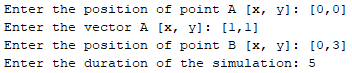
\includegraphics[]{images/input_pursuit_curve.png}}
    \begin{minipage}{0.45\textwidth}
        \centering
        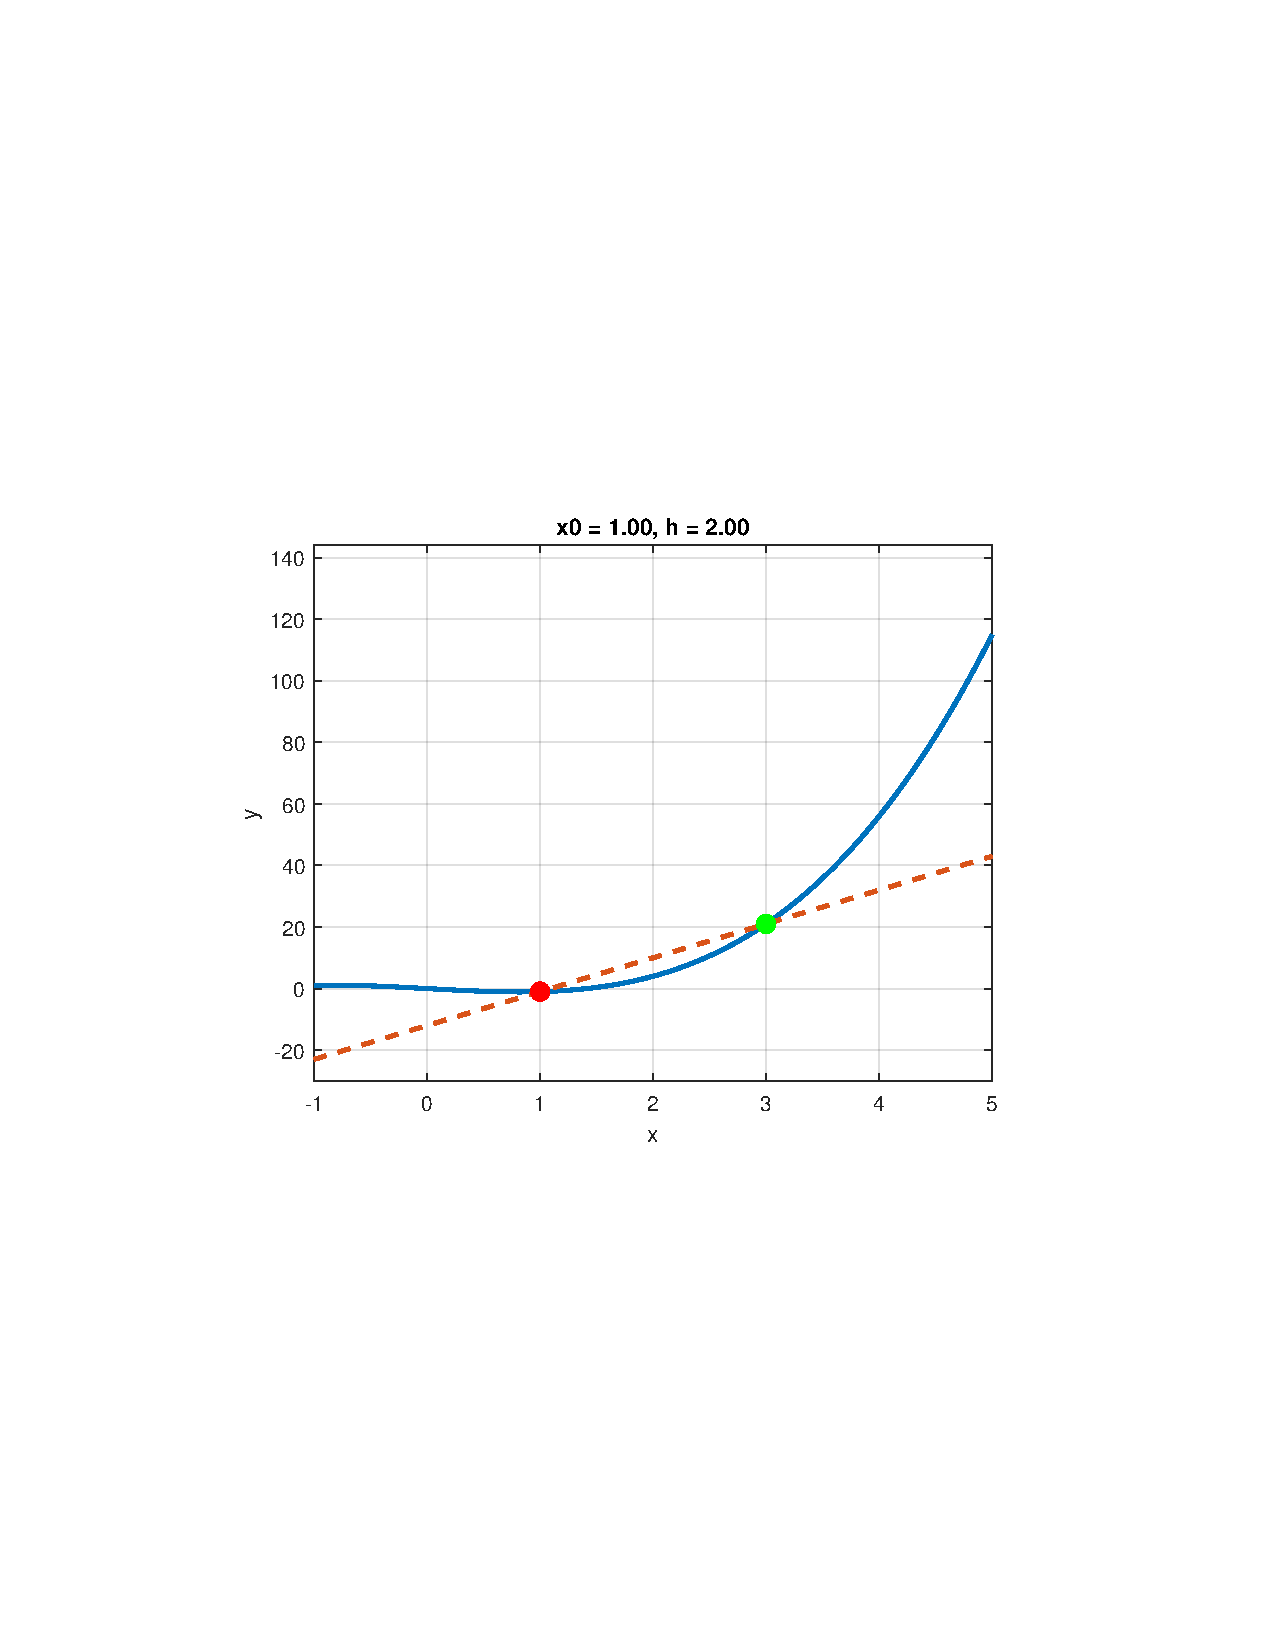
\includegraphics[trim={4.5cm 8.35cm 3.25cm 8cm},clip,scale=0.6]{pdfs/derivative.pdf}
        \caption{Initial state}
    \end{minipage}\hfill
    \begin{minipage}{0.45\textwidth}
        \centering
        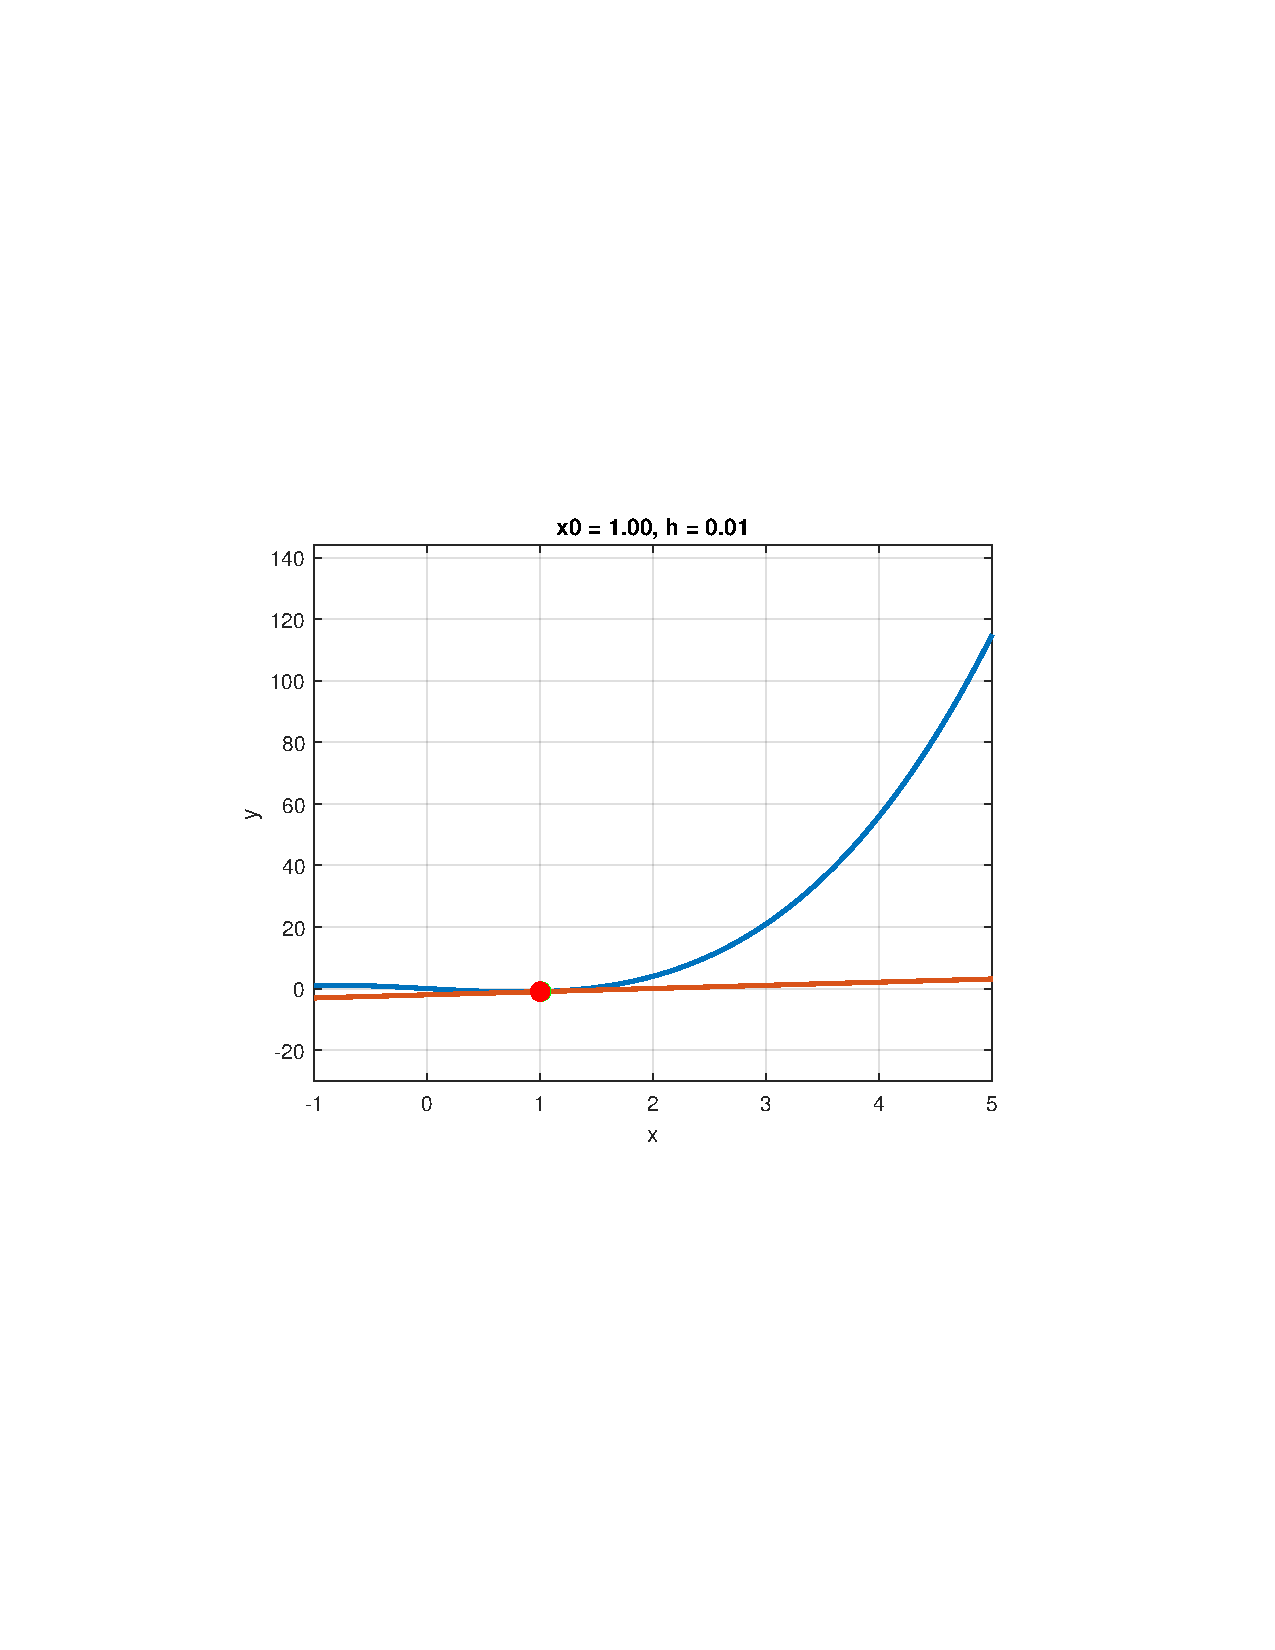
\includegraphics[trim={4.5cm 8.35cm 3.25cm 8cm},clip,scale=0.6]{pdfs/derivative_1.pdf}
        \caption{Final state}
    \end{minipage}
\end{figure}

The derivative provides crucial information about the behavior of functions in various fields, such as physics, economics, engineering, and more. It enables us to study and model dynamic systems, optimize functions, analyze rates of change, and understand fundamental properties of functions. The power of the derivative lies in its ability to capture instantaneous behavior and provide valuable insights into the intricate details of mathematical functions.

\newpage
\subsection{Applications}
% \subsu>bsection{Business and Economics}

% In recent years, economic decision making has become increasingly reliant on mathematical methods due to the abundance of statistical data and numerous variables involved. Business analysts and economists have turned to calculus to help describe and predict outcomes, as well as make informed decisions among various possibilities. In this context, we focus on the theory of the firm, which involves studying the activities of a business or industry during a period of relative stability in background conditions. We demonstrate how derivatives play a crucial role in aiding management with important production decisions. It is worth noting that even without an explicit understanding of calculus, management utilizes various functions similar to those we have discussed. Examples of such functions are:\\[-1.25cm]

% $$
% \begin{aligned}
% C(x) &: \text{cost of producing x units of the product},\\
% R(x) &: \text{revenue generated by selling x units of the product},\\
% P(x) &= R(x) - C(x) : \text{the profit (or loss) from producing and selling x units of the product.}
% \end{aligned}
% $$
% \subsubsection{Control Systems}

% In engineering, control systems are used to regulate and maintain desired behavior in various processes. These systems rely on feedback control, where measurements or observations of the system's output are continuously compared to a desired reference value. The resulting error is used to adjust the system's inputs or parameters to reduce the error and bring the system closer to the desired state.

% Derivatives play a critical role in feedback control by providing information about the rate of change of the error. This information allows control systems to respond effectively to changes in the system and improve stability and performance. The derivative term is particularly useful in predicting the future behavior of the system and can assist in damping oscillations and reducing settling time.

% One commonly used control strategy that incorporates derivatives is the Proportional-Integral-Derivative (PID) controller. A PID controller combines three components: proportional, integral, and derivative. While all three components are important, let's focus on the derivative component and its role in control systems.

% The derivative component of a PID controller calculates the derivative of the error signal. The error signal represents the difference between the system's output and the desired reference value. By taking the derivative of this error, the controller gains insight into the rate at which the error is changing over time. This information helps the controller make adjustments to the system's inputs or parameters.

\subsubsection{Electronic Speedometer}

An electronic speedometer is a key component in modern vehicles, providing drivers with real-time speed information. It relies on wheel speed sensors that generate electrical signals corresponding to the rotation of the wheels. By counting the pulses from these sensors within a specific time interval, the electronic control unit (ECU) calculates the derivative of the pulse count, which represents the rate of change of wheel speed. This derivative value is then converted into a speed measurement using calibration parameters and scaling factors. The final speed value is displayed on the speedometer's digital or analog display, ensuring that drivers have accurate and instantaneous speed readings.\\[0.1cm]

\begin{center}
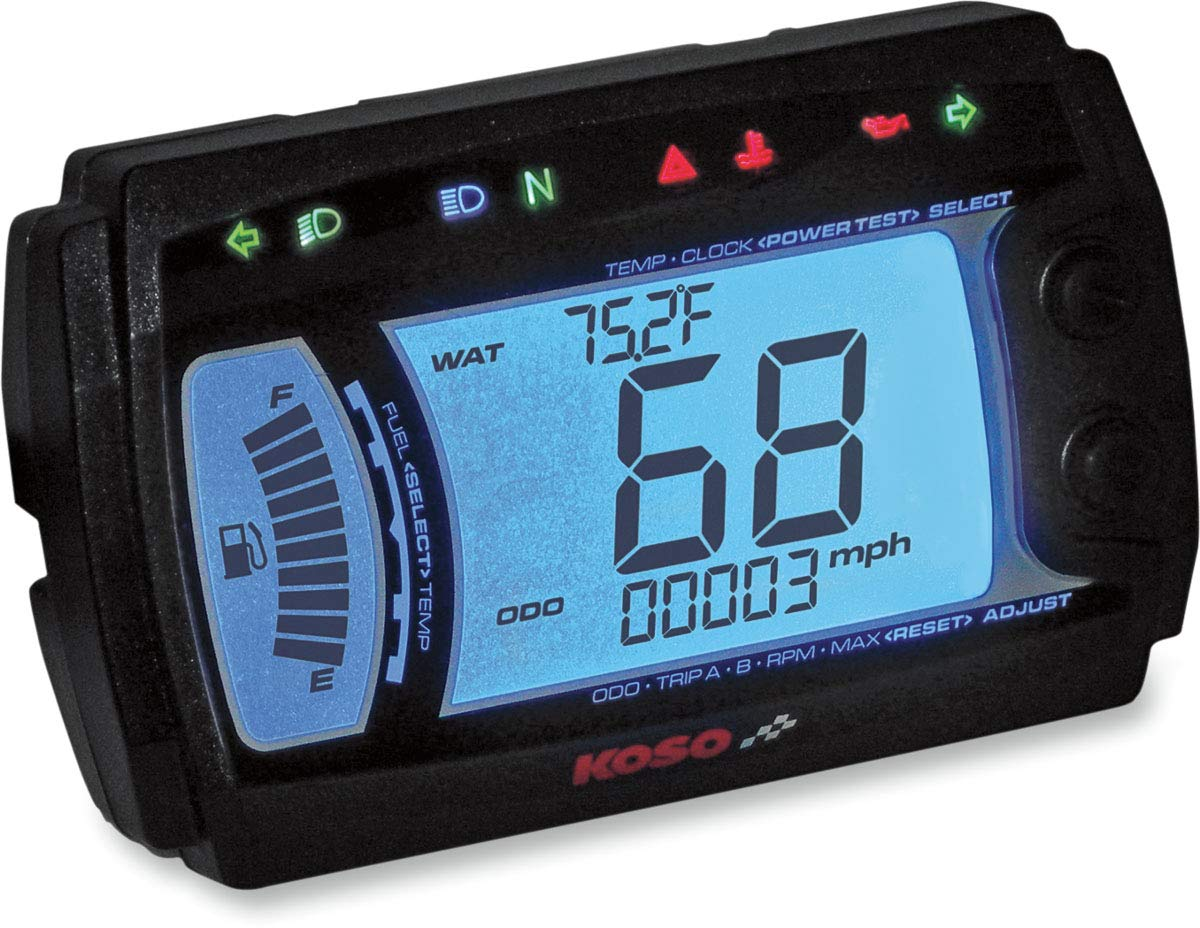
\includegraphics[width=.45\textwidth]{images/electronic_speedometer.jpg}
\end{center}

To ensure accurate readings, electronic speedometers often employ smoothing and filtering techniques. These techniques involve processing the derivative values to reduce noise and fluctuations caused by variations in wheel rotation. Filtering algorithms such as moving average or low-pass filters are applied to obtain a smoother representation of the speed. This helps drivers perceive a more stable speed reading, particularly in situations where wheel rotation may be inconsistent.

Overall, the application of derivatives in electronic speedometers enables the continuous monitoring and calculation of vehicle speed. By leveraging the principles of calculus, electronic speedometers provide drivers with reliable and up-to-date speed information, enhancing safety and enabling better control of the vehicle. Through the integration of wheel speed sensors, signal processing units, and display mechanisms, electronic speedometers ensure that drivers stay informed about their current speed while driving.

\subsubsection{Volume vs. Current in Capacitor}
The derivative of a capacitor represents how its voltage changes with respect to time. A capacitor is an electronic component that stores electrical energy in the form of an electric field. It consists of two conductive plates separated by an insulating material, known as a dielectric.

\begin{center}
\begin{circuitikz}
\ctikzset{capacitors/width=0.1}
\node[spdt, xscale=-1] (sw) {};
\draw   (sw.in)     node[above] {S}
                -- ++ (1,0)
                to [C=$C_1$, name=Csign] ++ (0,-3)  coordinate (aux1)
    (Csign.north west) node[above] {$+$}
    (Csign.north west) node[below=1mm] {$-$}
    (sw.out 2)  node[below] {b}   
                -- ++ (-0.5,0)          coordinate (aux2)
                to [R=$R_2$, -*]    (aux1 -| aux2)
    (sw.out 1)  node[above] {a}   
                to [R=$R_1$] ++ (-3,0)  coordinate (aux3)
                to [battery2, v_=$\epsilon$]    (aux3 |- aux1)
                -- (aux1);
\end{circuitikz}
\end{center}

When a voltage is applied across the capacitor, the plates accumulate opposite charges, creating an electric field between them. The voltage across the capacitor is directly proportional to the amount of charge stored on the plates. Mathematically, we can express this relationship as:

$$Q = C V$$

where $Q$ is the charge stored on the capacitor, $C$ is the capacitance (a measure of the capacitor's ability to store charge), and $V$ is the voltage across the capacitor.

Now, let's differentiate both sides of the equation with respect to time $t$:

$$\dfrac{dQ}{dt}=C\dfrac{dV}{dt}$$

The left side of the equation $\dfrac{dQ}{dt}$ represents the rate of change of charge with respect to time, which is the current flowing into or out of the capacitor. The right side of the equation $C\dfrac{dV}{dt}$ represents the capacitance multiplied by the rate of change of voltage with respect to time.

In other words, the derivative of a capacitor's voltage $\dfrac{dV}{dt}$ multiplied by its capacitance $C$ gives you the current flowing through the capacitor. This relationship is known as the capacitor current-voltage relationship.

In practice, when you apply a changing voltage across a capacitor (for example, in an AC circuit), the derivative of the voltage waveform determines the current flowing through the capacitor. The derivative $\dfrac{dV}{dt}$ represents the slope of the voltage waveform, indicating how quickly the voltage is changing at any given time. The capacitance $C$ determines how much current is required to change the voltage at a particular rate.

\begin{center}
\textcolor{black}{\fboxrule=2pt\fbox{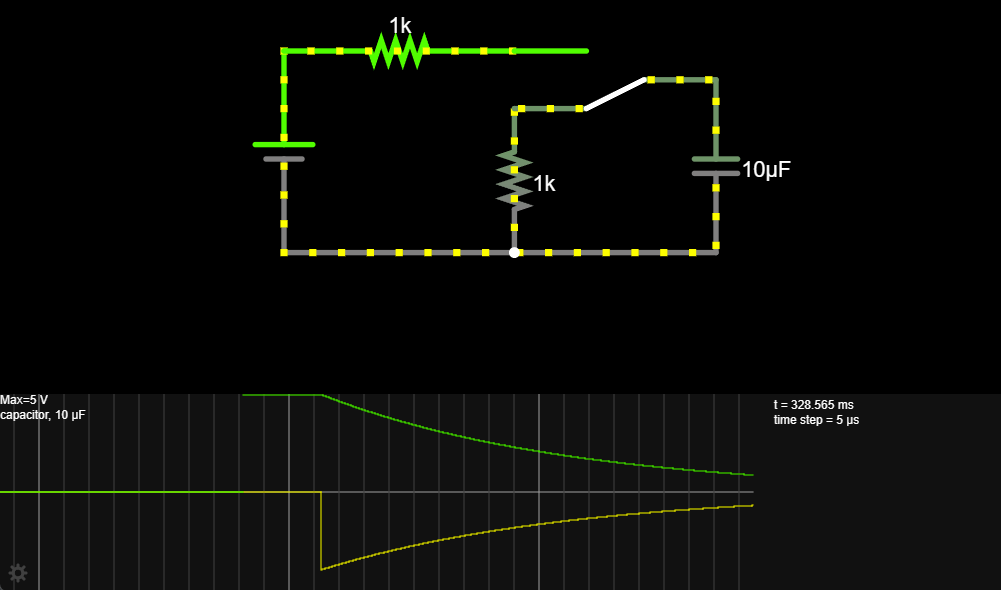
\includegraphics[width=.85\textwidth]{images/rc_circuit.png}}}
\end{center}

Taking this example, after the capacitor fully charged, let's define the time $t_0=0$ as the time when we switch the switch in the other direction, and $V(t_0)$ currently reaches its maximum. As the capacitor discharges, the function $V(t)$ gradually decreases to 0, following the plot of the exponential function $V(t)=e^{-ax}$. With the same duration, the current is given by $I(t)=C\dfrac{dV}{dt}=-Cae^{-ax}$.

It's important to note that the derivative of the voltage across a capacitor is discontinuous when the voltage suddenly changes, such as during the charging or discharging of the capacitor. At those instances, the derivative approaches infinity momentarily, indicating a high current flow.








\newpage
\section{Integral}
\subsection{Theoretical Basis}
Integrals are one of the fundamental concepts in mathematics and are used extensively in many fields of science and engineering. An integral is a mathematical representation of the area under a curve, and it provides a powerful tool for solving a wide range of problems.

The concept of integrals was first introduced in the \nth{17} century by mathematicians such as Isaac Newton\footnote{Issac Newton: \url{https://en.wikipedia.org/wiki/Isaac_Newton}} and Gottfried Wilhelm Leibniz\footnote{Gottfried Wilhelm Leibniz: \url{https://en.wikipedia.org/wiki/Gottfried_Wilhelm_Leibniz}}. The integral is represented by the following formula:

$$\int_a^b f(x)dx=F(x)\bigg|_a^b=F(b)-F(a)$$

Since its inception, the concept of integrals become a cornerstone of modern mathematics. Integrals have been used in many fields, including engineering, physics, economics, biology, computer science, and music theory.

To gain a clear understanding of integrals, the Riemann sum\footnote{Riemann sum: \url{https://en.wikipedia.org/wiki/Riemann_sum}} is a technique used to approximate their values by dividing the area under a curve into smaller rectangles. This method provides an estimation by summing the areas of these rectangles, with each rectangle's width and height determined by the partitioning of the interval and the function's evaluation at specific points. As the number of rectangles increases, the approximation becomes more accurate, approaching the exact value of the integral. The Riemann sum holds a foundational role in integral calculus and plays a crucial part in comprehending advanced integration methods.

Now, let's examine the Python code we have developed to demonstrate the Riemann sum approximation for the area under a curve. The code includes a slider that controls the number of rectangles used to approximate the area. This allows us to observe the convergence of the Riemann sum approximation towards the exact area:\\[-0.3cm]

\begin{minted}{python}
import numpy as np
import matplotlib.pyplot as plt
from matplotlib.widgets import Slider

# User input for f(x) function
try:
    fx = input("Enter the function f(x): ")
    f = lambda x: eval(fx)
except Exception as e:
    print("Error:", e)
    print("Please enter a valid function expression.")

def riemann_sum(f, a, b, n):
    """Compute the Riemann sum for the function f over the interval [a, b]"""
    dx = (b - a) / n  # Width of each subinterval
    x = np.linspace(a, b, n+1)  # Partition interval [a, b] into n subintervals
    heights = f(x[:-1])  # Heights of the rectangles using left endpoints
    total_area = np.sum(heights) * dx  # Sum the areas of all rectangles
    return total_area

# Define interval [a, b] and number of subintervals (n)
while True:
    try:
        a, b = map(float, input("Enter the domain values for a and b: ").split())
        break
    except ValueError:
        print("Invalid input. Please enter valid numeric values.")
        
n = 10

# Plotting the function
x = np.linspace(a, b, 10000)
y = f(x)

# Create the figure and the line
fig, ax = plt.subplots()
line, = ax.plot(x, y, lw=2)

plt.title('Riemann Sum: Approximation of Area under the Curve')

# Creating rectangles
x_bar = np.linspace(a, b, n+1)[:-1]
y_bar = f(x_bar + (b - a) / n)
bar = ax.bar(x_bar, y_bar, width=(b - a) / n, align='edge', alpha=0.3, edgecolor='k')
ax.set_xlabel('Time [s]')

total_area = np.trapz(y, x)
approx_area = riemann_sum(f, a, b, n)
error = total_area - approx_area
textString = f"Area = {total_area:.6f}\n~Area = {approx_area:.6f}\nError = {error:.6f}"
props = dict(boxstyle='round', facecolor='wheat', alpha=0.5)
text = ax.text(0.03, 0.95, textString, transform=ax.transAxes, fontsize=10,
        verticalalignment='top', bbox=props)

# Adjust main plot to make room for the slider
fig.subplots_adjust(bottom=0.25)

# Make a horizontal slider to control the precision
axfreq = fig.add_axes([0.25, 0.1, 0.65, 0.03])
freq_slider = Slider(
    ax=axfreq,
    label='Precision',
    valmin=3,
    valmax=100,
    valinit=n,
    valfmt='%0.0f'
)

# The function to be called anytime the slider's value changes
def update(val):
    global bar, approx_area, error, text
    n = int(val)
    x_bar = np.linspace(a, b, n+1)[:-1]
    y_bar = f(x_bar + (b - a) / n)
    bar.remove()
    bar = ax.bar(x_bar, y_bar, width=(b - a) / n, align='edge', alpha=0.3, edgecolor='k')

    approx_area = riemann_sum(f, a, b, n)
    error = total_area - approx_area
    textString = f"Area = {total_area:.6f}\n~Area = {approx_area:.6f}\nError = {error:.6f}"
    text.set_text(textString)

    fig.canvas.draw_idle()

freq_slider.on_changed(update)

plt.show()
\end{minted}

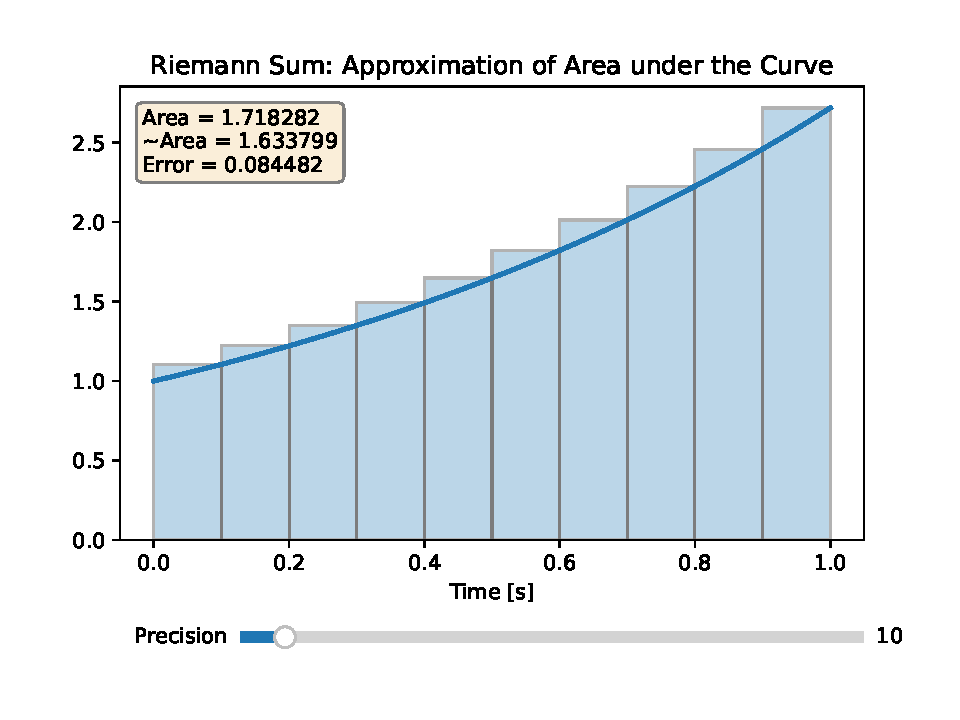
\includegraphics[trim={0.5cm 0.75cm 0 0.5cm},clip]{pdfs/riemann_sum.pdf}

In this report, we will explore the various applications of integrals in different fields. We will discuss how integrals are used to solve problems and provide examples of real-world applications. We will also examine the potential for future developments in the field of integral applications.

By the end of this report, readers will have a better understanding of the importance of integrals in various fields and will appreciate the versatility of this fundamental mathematical concept.

\newpage
\subsection{Applications}
\subsubsection{Physics}
Integrals can be used to calculate quantities such as area, volume, and work, and are an essential tool for modeling physical systems and analyzing their behavior. In the field of physics, integrals are particularly important for understanding the relationship between force and potential energy in conservative systems. By integrating the force function, we can obtain the corresponding potential energy function, and use it to gain insights into the behavior of the system.

For example, suppose we have a system where $F(x) = -kx$, where $k$ is a constant. We can find the corresponding potential energy function by integrating the force with respect to position:

\begin{gather*}
U(x) = -\int F(x) dx = -\int (-kx) dx = \frac{1}{2}kx^2 + C\\
\text{where } C \text{ is a constant of integration}
\end{gather*}

We can plot both the force and potential energy functions to compare them. Here is an example plot for the case where $k=1$ and $C=0$:

\begin{figure}[ht]
\centering
\hspace{0.5cm}\begin{minipage}{0.45\textwidth}
\centering
\begin{tikzpicture}[line cap=round,line join=round,>=triangle 45,x=1cm,
y=1cm]
% Vẽ 2 trục, điền các số lên trục
\draw[->] (-3.08,0) -- (3.06,0);
\foreach \x in {-2,2}
\draw[shift={(\x,0)},color=black] (0pt,2pt) -- (0pt,-2pt) 
node[below] { $\x$};
\draw[->,color=black] (0,-2) -- (0,3.98);
% \foreach \y in {-1}
% \draw[shift={(0,\y)},color=black] (2pt,0pt) -- (-2pt,0pt) 
% node[left] {\normalsize $\y$};
\draw[color=black] (2.8,.3) node[right] {$x$};
\draw[color=black] (.125,3.8) node[right] {\normalsize $y$};
\draw[color=black] (0pt,-8pt) node[left] {\normalsize $O$};
\clip(-3.08,-1.5) rectangle (3.1,3.25);
%Vẽ đồ thị
\draw[smooth,samples=100,domain=-4.08:2.06] 
plot(\x,{-(\x)});
% Vẽ thêm mấy cái râu ria
\draw[dashed] (1,0) -- (1,-1) -- (0,-1);
\draw[dashed] (0,2) -- (-2,2) -- (-2,0);
\node at (1,0.3) {$1$};
\node at (0.3,2) {$2$};
\node at (-0.3,-1) {$-1$};
\draw[shift={(0,3)},color=black] (2pt,0pt) -- (-2pt,0pt);
\node at (0.3,3) {$3$};
\node at (-1.75,3) {$F(x)=-x$};
\draw (0,0.2) -- (0.2,0.2) -- (0.2,0);
%Vẽ dấu chấm tròn 
\fill (0cm,0cm) circle (1.5pt); 
\fill (1,-1) circle (1.5pt); 
\fill (-2,2) circle (1.5pt); 
\end{tikzpicture}
\end{minipage}
\hfill
\begin{minipage}{0.45\textwidth}
\centering
\hspace{-1cm}\begin{tikzpicture}[line cap=round,line join=round,>=triangle 45,x=1cm,
y=1cm]
% Vẽ 2 trục, điền các số lên trục
\draw[->] (-3.08,0) -- (3.06,0);
\foreach \x in {-2,-1,1,2}
\draw[shift={(\x,0)},color=black] (0pt,2pt) -- (0pt,-2pt) 
node[below] { $\x$};
\draw[->,color=black] (0,-2) -- (0,3.98);
\foreach \y in {-1,1,3}
\draw[shift={(0,\y)},color=black] (2pt,0pt) -- (-2pt,0pt) 
node[left] {\normalsize $\y$};
\draw[color=black] (2.8,.3) node[right] {$x$};
\draw[color=black] (.125,3.8) node[right] {\normalsize $y$};
\draw[color=black] (0pt,-8pt) node[left] {\normalsize $O$};
\clip(-3.08,-1.5) rectangle (3.1,3.5);
%Vẽ đồ thị
\draw[smooth,samples=100,domain=-4.08:2.25] 
plot(\x,{((\x)^2)/2});
% Vẽ thêm mấy cái râu ria
\draw[dashed] (2,0) -- (2,2) -- (-2,2) -- (-2,0);
\node at (0.3,2.3) {$2$};
\node at (2,3) {$U(x)=\dfrac{x^2}{2}$};
\draw (0,0.2) -- (0.2,0.2) -- (0.2,0);
%Vẽ dấu chấm tròn 
\fill (0cm,0cm) circle (1.5pt); 
\fill (2,2) circle (1.5pt); 
\fill (-2,2) circle (1.5pt); 
\end{tikzpicture}
\end{minipage}
\caption{Force function and potential energy function for a one-dimensional system.}
\end{figure}

As we can see from the plot, the force function is linear and the potential energy function is quadratic. The potential energy function is minimum at $x=0$, which is the equilibrium position where the force is zero.

This example demonstrates how integrals can be used to analyze the relationship between force and potential energy in a physical system. By knowing the force, we can integrate to find the corresponding potential energy function and gain insights into the behavior of the system.

% \newpage
\subsubsection{Computer Graphics}
Double integrals are a powerful tool in mathematics and have numerous applications in various fields, including computer graphics. One of these applications is in the calculation of volumes under curved surfaces. In computer graphics, double integrals can be used to calculate the volume under a 3D curve that is defined by a function of two variables, such as $z = f(x, y)$. This calculation is essential in creating 3D models, simulations, and animations. By using double integrals, computer graphic designers and animators can accurately calculate the volume under the surface of a 3D model, which is critical in creating realistic and accurate visual representations.

\begin{figure}[ht]
\begin{minipage}{0.515\textwidth}
%
\centering
\tdplotsetmaincoords{70}{110}
%
% \hspace{-1cm}
\begin{tikzpicture}[tdplot_main_coords,scale=1.75]
	\tikzmath{function f(\x,\y) {return 1.5 + 0.5 * cos((0.5*\x + 0.75*\y) r);};}
	\pgfmathsetmacro{\step}{pi/50.0}
	\pgfmathsetmacro{\n}{8} % number of subinterals
	\pgfmathsetmacro{\dx}{0.25}	% 
	\pgfmathsetmacro{\dy}{0.25}	% 
	\pgfmathsetmacro{\xi}{0}	% initial value of the domain for the x variable
	\pgfmathsetmacro{\xf}{1.0*pi}	% final value of the domain for the x variable
	\pgfmathsetmacro{\xe}{\xf+\step}	%	next value in the domain of the plot of the function
	\pgfmathsetmacro{\xs}{\xi+\step} %	next value in the domain of the plot of the function
	\pgfmathsetmacro{\yi}{0}	% initial value of the domain for the y variable
	\pgfmathsetmacro{\yf}{1.0*pi}	% final value of the domain for the y variable
	\pgfmathsetmacro{\ys}{\yi+\step}	% next value in the domain of the plot of the function
	\pgfmathsetmacro{\ye}{\yf+\step}	%	next value in the domain of the plot of the function
	\pgfmathsetmacro{\h}{2.0}	% domain for the z-axis.
	% Limits of the region in the xy plane
	\pgfmathsetmacro{\a}{0.75}	% range for the x interval [a, b]
	\pgfmathsetmacro{\b}{\a+\n * \dx}	% range for the x interval [a, b]
	\pgfmathsetmacro{\c}{0.5}	% range for the y interval [c, d]
	\pgfmathsetmacro{\d}{\c+\n * \dx}	% range for the y interval [c, d]
	% Next point in the grid for the cycles \foreach
	\pgfmathsetmacro{\as}{\a+\dx}	% second value in the domain of the Riemann sum for the x variable
	\pgfmathsetmacro{\cs}{\c+\dy}	% second value in the domain of the Riemann sum for the x variable
	\pgfmathsetmacro{\ba}{\b-\dy}	% last value in the domain of the Riemann sum for the x variable
	\pgfmathsetmacro{\da}{\d-\dy}	% last value in the domain of the Riemann sum for the x variable
	% The coordinate axis
	\draw[thick,->] (\xi-0.25,0,0) -- (\xf+0.1,0,0) node [below] {$x$}; % x axis
	\draw[thick,->] (0,\yi-0.25,0) -- (0,\yf+0.1,0) node [right] {$y$}; % y axis
	\draw[thick,->] (0,0,0) -- (0,0,\h+0.25,0) node [above] {$z = f(x,y)$}; 
	% Grid of size \dx, \dy
	\foreach \x in {\a,\as,...,\b}
		\draw[very thin] (\x,\c,0) -- (\x,\d,0);
	\foreach \y in {\c,\cs,...,\d}
		\draw[very thin] (\a,\y,0) -- (\b,\y,0);
	% The region
	\draw[white] (\a,\d,0) -- (\b,\d,0) node [black,below,sloped,midway] {$R$};
	\fill[gray!25] (\a,\c,0) -- (\b,\c,0) -- (\b,\d,0) -- (\a,\d,0) -- (\a,\c,0);
	\draw[very thin] (\a,\c,0) -- (\b,\c,0) -- (\b,\d,0) -- (\a,\d,0) -- (\a,\c,0);
	% The graphs on the surface that delimit the region of integration
	\draw[blue,thick,opacity=0.75] plot[domain=\c:\d,smooth,variable=\t] ({\a},{\t},{f(\a,\t)});
	\draw[blue,thick,opacity=0.5] plot[domain=\a:\b,smooth,variable=\t] ({\t},{\c},{f(\t,\c)});
	% Riemann double sum
	\foreach \x in {\a,\as,...,\ba}{
		\foreach \y in {\c,\cs,...,\da}{
			\pgfmathsetmacro{\px}{\x}
			\pgfmathsetmacro{\py}{\y}
			\pgfmathsetmacro{\zdA}{f(\px,\py)}
			% Differential of area dA
			\draw[fill=cyan,opacity=0.25] (\px,\py,0) -- (\px,\py+\dy,0) -- (\px+\dx,\py+\dy,0) -- (\px+\dx,\py,0) -- (\px,\py,0);			
			% Boundary of the differential of volume
			\draw[ultra thin,opacity=0.35] (\px,\py,0) -- (\px,\py,\zdA);
			% Face parallel to the yz plane 
			\fill[cyan,opacity=0.35] 
				(\px+\dx,\py,0) -- (\px+\dx,\py,\zdA) -- (\px+\dx,\py+\dy,\zdA) 
				-- (\px+\dx,\py+\dy,0) -- (\px+\dx,\py,0);
			% Face parallel to the xz plane
			\fill[cyan,opacity=0.35] 
				(\px,\py+\dy,0) -- (\px,\py+\dy,\zdA) -- (\px+\dx,\py+\dy,\zdA) 
				-- (\px+\dx,\py+\dy,0) -- (\px+\dx,\py+\dy,0);
			\draw[thin] (\px+\dx,\py,0) -- (\px+\dx,\py,\zdA);
			\draw[thin] (\px,\py+\dy,0) -- (\px,\py+\dy,\zdA);
			\draw[thin,opacity=0.35] (\px+\dx,\py+\dy,0) -- (\px+\dx,\py+\dy,\zdA);
			\draw[thin,opacity=0.35] (\px+\dx,\py,0) -- (\px+\dx,\py+\dy,0);
			\draw[thin,opacity=0.35] (\px,\py+\dy,0) -- (\px+\dx,\py+\dy,0);
			\draw[fill=cyan,opacity=0.5,draw=black] (\px,\py,\zdA) -- (\px+\dx,\py,\zdA) 
					-- (\px+\dx,\py+\dy,\zdA) -- (\px,\py+\dy,\zdA) -- (\px,\py,\zdA);
			\draw[thin,opacity=0.35] (\px+\dx,\py+\dy,0) -- (\px+\dx,\py+\dy,\zdA);
			\draw[thin,opacity=0.35](\px,\py,\zdA) -- (\px+\dx,\py,\zdA) 
					-- (\px+\dx,\py+\dy,\zdA) -- (\px,\py+\dy,\zdA) -- (\px,\py,\zdA);
		}
	}
	% The surface: Quadrant I
	\foreach \x in {0,\step,...,\xf}{
		\draw[blue,opacity=0.25] plot[domain=0:\yf,smooth,variable=\t] ({\x},{\t},{f(\x,\t)});
	}
	\foreach \y in {0,\step,...,\yf}{
		\draw[blue,opacity=0.25] plot[domain=0:\yf,smooth,variable=\t] ({\t},{\y},{f(\t,\y)});
	}
	% 
	% The graphs on the surface that delimit the region of integration
	\draw[blue,thick,opacity=0.75] plot[domain=\c:\d,smooth,variable=\t] ({\b},{\t},{f(\b,\t)});
	\draw[blue,thick,opacity=0.75] plot[domain=\a:\b,smooth,variable=\t] ({\t},{\d},{f(\t,\d)});
\end{tikzpicture}
% \captionsetup{format=labelstyle, justification=raggedright}
\caption{Double integral virtualization}
\end{minipage}
\begin{minipage}{0.45\textwidth}
    \centering
    \vspace{0.5cm}
    Volume under $f(x,y)$ bounded by a given region $R$ defined by $x\in\left[a,b\right]$ and $y\in\left[c,d\right]$ is
    $$\iint_R f(x,y)dA=\int_a^b\int_c^d f(x,y)\;dy\;dx$$
    $$\text{where}\ dA=dx\;dy$$
\end{minipage}
\end{figure}

To enhance the exploration and understanding of various functions, we have developed a Python code that allows users to input functions in terms of $x$ and $y$, as well as define the corresponding domains. Running the program enables users to visualize the function's graph and wireframe volume, providing valuable insights into its properties. This interactive simulation offers a dynamic and visually engaging platform to analyze and gain a deeper comprehension of diverse functions. Below is the code:\\[-0.3cm]

\begin{minted}{python}
import numpy as np
import matplotlib.pyplot as plt

# User input for f(x) function
try:
    fxy = input("Enter the function f(x, y): ")
    f = lambda x, y: eval(fxy)
except Exception as e:
    print("Error:", e)
    print("Please enter a valid function expression.")

def simulate_double_integral():
    """Simulates a double integral and plots the result"""
    while True:
        try:
            x_min, x_max = map(float, input("Enter x-min and x-max (space-separated): ").split())
            y_min, y_max = map(float, input("Enter y-min and y-max (space-separated): ").split())
            break
        except ValueError:
            print("Invalid input. Please enter valid numeric values.")

    num_points = 100  # Number of points in each dimension

    x = np.linspace(x_min, x_max, num_points)
    y = np.linspace(y_min, y_max, num_points)
    X, Y = np.meshgrid(x, y)
    Z = f(X, Y)

    # Calculate the volume under the surface using the trapezoidal rule
    while True:
        try:
            volume = np.trapz(np.trapz(Z, dx=(x_max - x_min) / (num_points - 1), axis=0), dx=(y_max - y_min) / (num_points - 1))
            break
        except Exception as e:
            print("Error:", e)
            print("Please enter a valid function expression.")
            Z = f(X, Y)

    # Plotting the result
    fig = plt.figure()
    ax = fig.add_subplot(111, projection='3d')

    # 3D surface plot
    ax.plot_surface(X, Y, Z, cmap='viridis', alpha=1.0)
    ax.set_xlabel('X')
    ax.set_ylabel('Y')
    ax.set_zlabel('f(X, Y)')

    # Set the z-axis limits based on function values
    z_min, z_max = np.min(Z), np.max(Z)
    if z_min >= 0:
        ax.set_zlim(0, z_max)
    elif z_max <= 0:
        ax.set_zlim(z_min, 0)
    else:
        ax.set_zlim(z_min, z_max)

    # Rotate the camera to a different view
    ax.view_init(elev=30, azim=45) 

    # Projection on XY-plane
    ax.contourf(X, Y, Z, zdir='z', offset=0, cmap='viridis', alpha=0.3)

    # Draw dashed lines from surface to base
    ax.plot([x_min, x_min], [y_min, y_min], [0, Z[0, 0]], 'k--')
    ax.plot([x_max, x_max], [y_min, y_min], [0, Z[0, -1]], 'k--')
    ax.plot([x_min, x_min], [y_max, y_max], [0, Z[-1, 0]], 'k--')
    ax.plot([x_max, x_max], [y_max, y_max], [0, Z[-1, -1]], 'k--')

    # Draw boundary dashed lines
    ax.plot(x, y_min * np.ones_like(x), zs=0, linestyle='dashed', color='black')
    ax.plot(x, y_max * np.ones_like(x), zs=0, linestyle='dashed', color='black')
    ax.plot(x_min * np.ones_like(y), y, zs=0, linestyle='dashed', color='black')
    ax.plot(x_max * np.ones_like(y), y, zs=0, linestyle='dashed', color='black')

    plt.title(f"Volume: {volume:.6f}")
    plt.show()

# Run the simulation
simulate_double_integral()
\end{minted}

Input and Result:\\[-0.35cm]
\begin{center}
\efbox{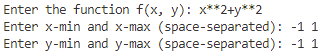
\includegraphics[]{images/input_double_integral.png}}
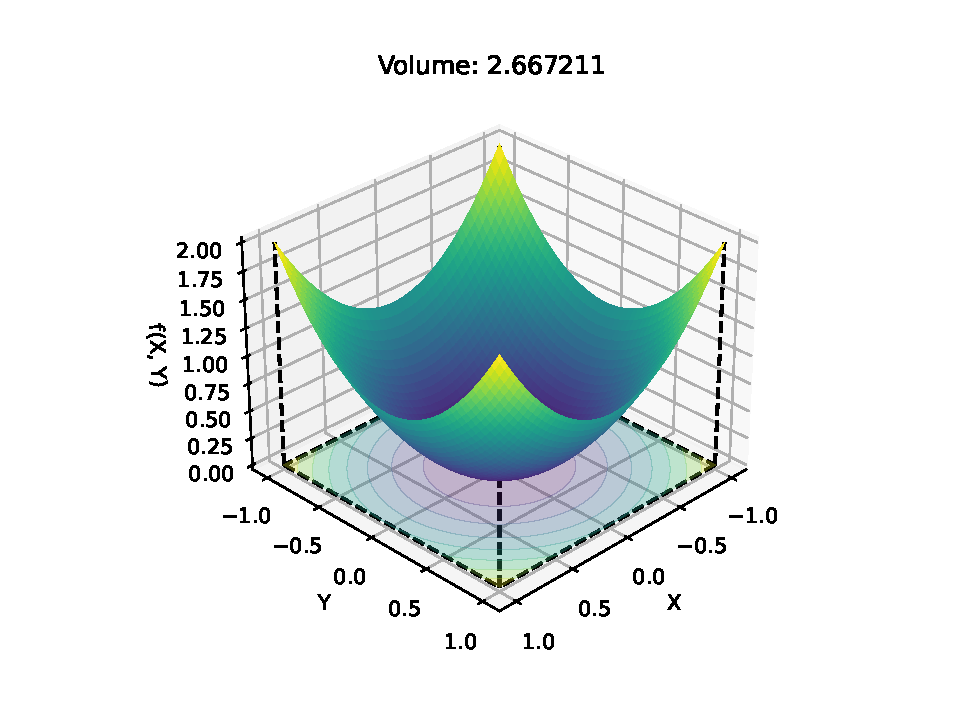
\includegraphics[trim={0.5cm 1cm 0 0.35cm},clip]{pdfs/double_integral.pdf}
\end{center}


Moreover, the more advanced tool, triple integrals, is even more powerful than double integrals, as they can calculate volumes of 3D objects that are more complex. Triple integrals can integrate over a region in 3D space, whereas double integrals can integrate only on a 2D plane. In summary, both double and triple integrals are powerful mathematical tools with numerous real-world applications, especially in fields such as computer graphics.





% \newpage
\subsubsection{Signal Processing}

Integrals are a fundamental mathematical tool used in many engineering applications, particularly in the analysis of signals and systems. One important application of integrals is in the field of audio engineering, where they are used to analyze and manipulate sound signals. The Fourier Transform is a mathematical technique that uses integrals to extract frequency components of a signal, and it is widely used in audio engineering.

The Fourier Transform is a widely used algorithm for calculating the Fourier Transform of discrete-time signals. It is used to plot the amplitude of sound waves as a function of frequency. Engineers use Fourier Transform to sample the sound signal at regular intervals, then apply the algorithm to the signal, which calculates the amplitude of the signal at different frequencies. The resulting plot shows the amplitude of the signal at each frequency, allowing engineers to identify the different frequency components of the sound wave.

Continuous-time Fourier Transform have this basic formula:

\begin{gather*}
X(f)=\int_{-\infty}^{\infty} x(t)e^{-j2\pi ft} dt\\
\text{where } f \text{ is the frequency, } x(t) \text{ is signal with respect to time}
\end{gather*}

To simplify the process, we utilize an external Python package in our Python code to simulate the sound wave using the Fast Fourier Transform:\\[-0.3cm]

\begin{minted}{Python}
import matplotlib.pyplot as plt
import numpy as np
from scipy.fftpack import fft
from scipy.io import wavfile

sr, data = wavfile.read('sample.wav')
print(data.shape, sr)
signal = data[:sr,0]
Signal = fft(signal)
fig, (axt, axf) = plt.subplots(2, 1, constrained_layout=1, figsize=(11.8,3))
axt.plot(signal, lw=0.15) ; axt.grid(1)
axf.plot(np.abs(Signal[:sr//2]), lw=0.15) ; axf.grid(1)
plt.show()
\end{minted}

% \begin{tikzpicture}[samples=200, domain=0:5*360]
%         \begin{axis}[
%             width=10cm, height=4cm,
%             enlarge x limits=false,
%             xtick=\empty,
%             axis lines*=middle,
%             hide y axis
%         ]
%         \addplot [no markers, smooth] {sin(x)+rand};
%         \end{axis}
%     \end{tikzpicture}

\vspace{0.45cm}

\begin{figure}[ht!]
    \begin{center}
        %% Creator: Matplotlib, PGF backend
%%
%% To include the figure in your LaTeX document, write
%%   \input{<filename>.pgf}
%%
%% Make sure the required packages are loaded in your preamble
%%   \usepackage{pgf}
%%
%% Also ensure that all the required font packages are loaded; for instance,
%% the lmodern package is sometimes necessary when using math font.
%%   \usepackage{lmodern}
%%
%% Figures using additional raster images can only be included by \input if
%% they are in the same directory as the main LaTeX file. For loading figures
%% from other directories you can use the `import` package
%%   \usepackage{import}
%%
%% and then include the figures with
%%   \import{<path to file>}{<filename>.pgf}
%%
%% Matplotlib used the following preamble
%%   
%%   \makeatletter\@ifpackageloaded{underscore}{}{\usepackage[strings]{underscore}}\makeatother
%%
\begingroup%
\makeatletter%
\begin{pgfpicture}%
\pgfpathrectangle{\pgfpointorigin}{\pgfqpoint{6.500000in}{3.500000in}}%
\pgfusepath{use as bounding box, clip}%
\begin{pgfscope}%
\pgfsetbuttcap%
\pgfsetmiterjoin%
\definecolor{currentfill}{rgb}{1.000000,1.000000,1.000000}%
\pgfsetfillcolor{currentfill}%
\pgfsetlinewidth{0.000000pt}%
\definecolor{currentstroke}{rgb}{1.000000,1.000000,1.000000}%
\pgfsetstrokecolor{currentstroke}%
\pgfsetdash{}{0pt}%
\pgfpathmoveto{\pgfqpoint{0.000000in}{0.000000in}}%
\pgfpathlineto{\pgfqpoint{6.500000in}{0.000000in}}%
\pgfpathlineto{\pgfqpoint{6.500000in}{3.500000in}}%
\pgfpathlineto{\pgfqpoint{0.000000in}{3.500000in}}%
\pgfpathlineto{\pgfqpoint{0.000000in}{0.000000in}}%
\pgfpathclose%
\pgfusepath{fill}%
\end{pgfscope}%
\begin{pgfscope}%
\pgfsetbuttcap%
\pgfsetmiterjoin%
\definecolor{currentfill}{rgb}{1.000000,1.000000,1.000000}%
\pgfsetfillcolor{currentfill}%
\pgfsetlinewidth{0.000000pt}%
\definecolor{currentstroke}{rgb}{0.000000,0.000000,0.000000}%
\pgfsetstrokecolor{currentstroke}%
\pgfsetstrokeopacity{0.000000}%
\pgfsetdash{}{0pt}%
\pgfpathmoveto{\pgfqpoint{0.594141in}{2.085466in}}%
\pgfpathlineto{\pgfqpoint{6.327930in}{2.085466in}}%
\pgfpathlineto{\pgfqpoint{6.327930in}{3.458330in}}%
\pgfpathlineto{\pgfqpoint{0.594141in}{3.458330in}}%
\pgfpathlineto{\pgfqpoint{0.594141in}{2.085466in}}%
\pgfpathclose%
\pgfusepath{fill}%
\end{pgfscope}%
\begin{pgfscope}%
\pgfpathrectangle{\pgfqpoint{0.594141in}{2.085466in}}{\pgfqpoint{5.733789in}{1.372864in}}%
\pgfusepath{clip}%
\pgfsetrectcap%
\pgfsetroundjoin%
\pgfsetlinewidth{0.803000pt}%
\definecolor{currentstroke}{rgb}{0.690196,0.690196,0.690196}%
\pgfsetstrokecolor{currentstroke}%
\pgfsetdash{}{0pt}%
\pgfpathmoveto{\pgfqpoint{0.854767in}{2.085466in}}%
\pgfpathlineto{\pgfqpoint{0.854767in}{3.458330in}}%
\pgfusepath{stroke}%
\end{pgfscope}%
\begin{pgfscope}%
\pgfsetbuttcap%
\pgfsetroundjoin%
\definecolor{currentfill}{rgb}{0.000000,0.000000,0.000000}%
\pgfsetfillcolor{currentfill}%
\pgfsetlinewidth{0.803000pt}%
\definecolor{currentstroke}{rgb}{0.000000,0.000000,0.000000}%
\pgfsetstrokecolor{currentstroke}%
\pgfsetdash{}{0pt}%
\pgfsys@defobject{currentmarker}{\pgfqpoint{0.000000in}{-0.048611in}}{\pgfqpoint{0.000000in}{0.000000in}}{%
\pgfpathmoveto{\pgfqpoint{0.000000in}{0.000000in}}%
\pgfpathlineto{\pgfqpoint{0.000000in}{-0.048611in}}%
\pgfusepath{stroke,fill}%
}%
\begin{pgfscope}%
\pgfsys@transformshift{0.854767in}{2.085466in}%
\pgfsys@useobject{currentmarker}{}%
\end{pgfscope}%
\end{pgfscope}%
\begin{pgfscope}%
\definecolor{textcolor}{rgb}{0.000000,0.000000,0.000000}%
\pgfsetstrokecolor{textcolor}%
\pgfsetfillcolor{textcolor}%
\pgftext[x=0.854767in,y=1.988244in,,top]{\color{textcolor}\rmfamily\fontsize{10.000000}{12.000000}\selectfont \(\displaystyle {0}\)}%
\end{pgfscope}%
\begin{pgfscope}%
\pgfpathrectangle{\pgfqpoint{0.594141in}{2.085466in}}{\pgfqpoint{5.733789in}{1.372864in}}%
\pgfusepath{clip}%
\pgfsetrectcap%
\pgfsetroundjoin%
\pgfsetlinewidth{0.803000pt}%
\definecolor{currentstroke}{rgb}{0.690196,0.690196,0.690196}%
\pgfsetstrokecolor{currentstroke}%
\pgfsetdash{}{0pt}%
\pgfpathmoveto{\pgfqpoint{1.940735in}{2.085466in}}%
\pgfpathlineto{\pgfqpoint{1.940735in}{3.458330in}}%
\pgfusepath{stroke}%
\end{pgfscope}%
\begin{pgfscope}%
\pgfsetbuttcap%
\pgfsetroundjoin%
\definecolor{currentfill}{rgb}{0.000000,0.000000,0.000000}%
\pgfsetfillcolor{currentfill}%
\pgfsetlinewidth{0.803000pt}%
\definecolor{currentstroke}{rgb}{0.000000,0.000000,0.000000}%
\pgfsetstrokecolor{currentstroke}%
\pgfsetdash{}{0pt}%
\pgfsys@defobject{currentmarker}{\pgfqpoint{0.000000in}{-0.048611in}}{\pgfqpoint{0.000000in}{0.000000in}}{%
\pgfpathmoveto{\pgfqpoint{0.000000in}{0.000000in}}%
\pgfpathlineto{\pgfqpoint{0.000000in}{-0.048611in}}%
\pgfusepath{stroke,fill}%
}%
\begin{pgfscope}%
\pgfsys@transformshift{1.940735in}{2.085466in}%
\pgfsys@useobject{currentmarker}{}%
\end{pgfscope}%
\end{pgfscope}%
\begin{pgfscope}%
\definecolor{textcolor}{rgb}{0.000000,0.000000,0.000000}%
\pgfsetstrokecolor{textcolor}%
\pgfsetfillcolor{textcolor}%
\pgftext[x=1.940735in,y=1.988244in,,top]{\color{textcolor}\rmfamily\fontsize{10.000000}{12.000000}\selectfont \(\displaystyle {10000}\)}%
\end{pgfscope}%
\begin{pgfscope}%
\pgfpathrectangle{\pgfqpoint{0.594141in}{2.085466in}}{\pgfqpoint{5.733789in}{1.372864in}}%
\pgfusepath{clip}%
\pgfsetrectcap%
\pgfsetroundjoin%
\pgfsetlinewidth{0.803000pt}%
\definecolor{currentstroke}{rgb}{0.690196,0.690196,0.690196}%
\pgfsetstrokecolor{currentstroke}%
\pgfsetdash{}{0pt}%
\pgfpathmoveto{\pgfqpoint{3.026702in}{2.085466in}}%
\pgfpathlineto{\pgfqpoint{3.026702in}{3.458330in}}%
\pgfusepath{stroke}%
\end{pgfscope}%
\begin{pgfscope}%
\pgfsetbuttcap%
\pgfsetroundjoin%
\definecolor{currentfill}{rgb}{0.000000,0.000000,0.000000}%
\pgfsetfillcolor{currentfill}%
\pgfsetlinewidth{0.803000pt}%
\definecolor{currentstroke}{rgb}{0.000000,0.000000,0.000000}%
\pgfsetstrokecolor{currentstroke}%
\pgfsetdash{}{0pt}%
\pgfsys@defobject{currentmarker}{\pgfqpoint{0.000000in}{-0.048611in}}{\pgfqpoint{0.000000in}{0.000000in}}{%
\pgfpathmoveto{\pgfqpoint{0.000000in}{0.000000in}}%
\pgfpathlineto{\pgfqpoint{0.000000in}{-0.048611in}}%
\pgfusepath{stroke,fill}%
}%
\begin{pgfscope}%
\pgfsys@transformshift{3.026702in}{2.085466in}%
\pgfsys@useobject{currentmarker}{}%
\end{pgfscope}%
\end{pgfscope}%
\begin{pgfscope}%
\definecolor{textcolor}{rgb}{0.000000,0.000000,0.000000}%
\pgfsetstrokecolor{textcolor}%
\pgfsetfillcolor{textcolor}%
\pgftext[x=3.026702in,y=1.988244in,,top]{\color{textcolor}\rmfamily\fontsize{10.000000}{12.000000}\selectfont \(\displaystyle {20000}\)}%
\end{pgfscope}%
\begin{pgfscope}%
\pgfpathrectangle{\pgfqpoint{0.594141in}{2.085466in}}{\pgfqpoint{5.733789in}{1.372864in}}%
\pgfusepath{clip}%
\pgfsetrectcap%
\pgfsetroundjoin%
\pgfsetlinewidth{0.803000pt}%
\definecolor{currentstroke}{rgb}{0.690196,0.690196,0.690196}%
\pgfsetstrokecolor{currentstroke}%
\pgfsetdash{}{0pt}%
\pgfpathmoveto{\pgfqpoint{4.112670in}{2.085466in}}%
\pgfpathlineto{\pgfqpoint{4.112670in}{3.458330in}}%
\pgfusepath{stroke}%
\end{pgfscope}%
\begin{pgfscope}%
\pgfsetbuttcap%
\pgfsetroundjoin%
\definecolor{currentfill}{rgb}{0.000000,0.000000,0.000000}%
\pgfsetfillcolor{currentfill}%
\pgfsetlinewidth{0.803000pt}%
\definecolor{currentstroke}{rgb}{0.000000,0.000000,0.000000}%
\pgfsetstrokecolor{currentstroke}%
\pgfsetdash{}{0pt}%
\pgfsys@defobject{currentmarker}{\pgfqpoint{0.000000in}{-0.048611in}}{\pgfqpoint{0.000000in}{0.000000in}}{%
\pgfpathmoveto{\pgfqpoint{0.000000in}{0.000000in}}%
\pgfpathlineto{\pgfqpoint{0.000000in}{-0.048611in}}%
\pgfusepath{stroke,fill}%
}%
\begin{pgfscope}%
\pgfsys@transformshift{4.112670in}{2.085466in}%
\pgfsys@useobject{currentmarker}{}%
\end{pgfscope}%
\end{pgfscope}%
\begin{pgfscope}%
\definecolor{textcolor}{rgb}{0.000000,0.000000,0.000000}%
\pgfsetstrokecolor{textcolor}%
\pgfsetfillcolor{textcolor}%
\pgftext[x=4.112670in,y=1.988244in,,top]{\color{textcolor}\rmfamily\fontsize{10.000000}{12.000000}\selectfont \(\displaystyle {30000}\)}%
\end{pgfscope}%
\begin{pgfscope}%
\pgfpathrectangle{\pgfqpoint{0.594141in}{2.085466in}}{\pgfqpoint{5.733789in}{1.372864in}}%
\pgfusepath{clip}%
\pgfsetrectcap%
\pgfsetroundjoin%
\pgfsetlinewidth{0.803000pt}%
\definecolor{currentstroke}{rgb}{0.690196,0.690196,0.690196}%
\pgfsetstrokecolor{currentstroke}%
\pgfsetdash{}{0pt}%
\pgfpathmoveto{\pgfqpoint{5.198638in}{2.085466in}}%
\pgfpathlineto{\pgfqpoint{5.198638in}{3.458330in}}%
\pgfusepath{stroke}%
\end{pgfscope}%
\begin{pgfscope}%
\pgfsetbuttcap%
\pgfsetroundjoin%
\definecolor{currentfill}{rgb}{0.000000,0.000000,0.000000}%
\pgfsetfillcolor{currentfill}%
\pgfsetlinewidth{0.803000pt}%
\definecolor{currentstroke}{rgb}{0.000000,0.000000,0.000000}%
\pgfsetstrokecolor{currentstroke}%
\pgfsetdash{}{0pt}%
\pgfsys@defobject{currentmarker}{\pgfqpoint{0.000000in}{-0.048611in}}{\pgfqpoint{0.000000in}{0.000000in}}{%
\pgfpathmoveto{\pgfqpoint{0.000000in}{0.000000in}}%
\pgfpathlineto{\pgfqpoint{0.000000in}{-0.048611in}}%
\pgfusepath{stroke,fill}%
}%
\begin{pgfscope}%
\pgfsys@transformshift{5.198638in}{2.085466in}%
\pgfsys@useobject{currentmarker}{}%
\end{pgfscope}%
\end{pgfscope}%
\begin{pgfscope}%
\definecolor{textcolor}{rgb}{0.000000,0.000000,0.000000}%
\pgfsetstrokecolor{textcolor}%
\pgfsetfillcolor{textcolor}%
\pgftext[x=5.198638in,y=1.988244in,,top]{\color{textcolor}\rmfamily\fontsize{10.000000}{12.000000}\selectfont \(\displaystyle {40000}\)}%
\end{pgfscope}%
\begin{pgfscope}%
\pgfpathrectangle{\pgfqpoint{0.594141in}{2.085466in}}{\pgfqpoint{5.733789in}{1.372864in}}%
\pgfusepath{clip}%
\pgfsetrectcap%
\pgfsetroundjoin%
\pgfsetlinewidth{0.803000pt}%
\definecolor{currentstroke}{rgb}{0.690196,0.690196,0.690196}%
\pgfsetstrokecolor{currentstroke}%
\pgfsetdash{}{0pt}%
\pgfpathmoveto{\pgfqpoint{6.284605in}{2.085466in}}%
\pgfpathlineto{\pgfqpoint{6.284605in}{3.458330in}}%
\pgfusepath{stroke}%
\end{pgfscope}%
\begin{pgfscope}%
\pgfsetbuttcap%
\pgfsetroundjoin%
\definecolor{currentfill}{rgb}{0.000000,0.000000,0.000000}%
\pgfsetfillcolor{currentfill}%
\pgfsetlinewidth{0.803000pt}%
\definecolor{currentstroke}{rgb}{0.000000,0.000000,0.000000}%
\pgfsetstrokecolor{currentstroke}%
\pgfsetdash{}{0pt}%
\pgfsys@defobject{currentmarker}{\pgfqpoint{0.000000in}{-0.048611in}}{\pgfqpoint{0.000000in}{0.000000in}}{%
\pgfpathmoveto{\pgfqpoint{0.000000in}{0.000000in}}%
\pgfpathlineto{\pgfqpoint{0.000000in}{-0.048611in}}%
\pgfusepath{stroke,fill}%
}%
\begin{pgfscope}%
\pgfsys@transformshift{6.284605in}{2.085466in}%
\pgfsys@useobject{currentmarker}{}%
\end{pgfscope}%
\end{pgfscope}%
\begin{pgfscope}%
\definecolor{textcolor}{rgb}{0.000000,0.000000,0.000000}%
\pgfsetstrokecolor{textcolor}%
\pgfsetfillcolor{textcolor}%
\pgftext[x=6.284605in,y=1.988244in,,top]{\color{textcolor}\rmfamily\fontsize{10.000000}{12.000000}\selectfont \(\displaystyle {50000}\)}%
\end{pgfscope}%
\begin{pgfscope}%
\pgfpathrectangle{\pgfqpoint{0.594141in}{2.085466in}}{\pgfqpoint{5.733789in}{1.372864in}}%
\pgfusepath{clip}%
\pgfsetrectcap%
\pgfsetroundjoin%
\pgfsetlinewidth{0.803000pt}%
\definecolor{currentstroke}{rgb}{0.690196,0.690196,0.690196}%
\pgfsetstrokecolor{currentstroke}%
\pgfsetdash{}{0pt}%
\pgfpathmoveto{\pgfqpoint{0.594141in}{2.393749in}}%
\pgfpathlineto{\pgfqpoint{6.327930in}{2.393749in}}%
\pgfusepath{stroke}%
\end{pgfscope}%
\begin{pgfscope}%
\pgfsetbuttcap%
\pgfsetroundjoin%
\definecolor{currentfill}{rgb}{0.000000,0.000000,0.000000}%
\pgfsetfillcolor{currentfill}%
\pgfsetlinewidth{0.803000pt}%
\definecolor{currentstroke}{rgb}{0.000000,0.000000,0.000000}%
\pgfsetstrokecolor{currentstroke}%
\pgfsetdash{}{0pt}%
\pgfsys@defobject{currentmarker}{\pgfqpoint{-0.048611in}{0.000000in}}{\pgfqpoint{-0.000000in}{0.000000in}}{%
\pgfpathmoveto{\pgfqpoint{-0.000000in}{0.000000in}}%
\pgfpathlineto{\pgfqpoint{-0.048611in}{0.000000in}}%
\pgfusepath{stroke,fill}%
}%
\begin{pgfscope}%
\pgfsys@transformshift{0.594141in}{2.393749in}%
\pgfsys@useobject{currentmarker}{}%
\end{pgfscope}%
\end{pgfscope}%
\begin{pgfscope}%
\definecolor{textcolor}{rgb}{0.000000,0.000000,0.000000}%
\pgfsetstrokecolor{textcolor}%
\pgfsetfillcolor{textcolor}%
\pgftext[x=0.041670in, y=2.345524in, left, base]{\color{textcolor}\rmfamily\fontsize{10.000000}{12.000000}\selectfont \(\displaystyle {\ensuremath{-}10000}\)}%
\end{pgfscope}%
\begin{pgfscope}%
\pgfpathrectangle{\pgfqpoint{0.594141in}{2.085466in}}{\pgfqpoint{5.733789in}{1.372864in}}%
\pgfusepath{clip}%
\pgfsetrectcap%
\pgfsetroundjoin%
\pgfsetlinewidth{0.803000pt}%
\definecolor{currentstroke}{rgb}{0.690196,0.690196,0.690196}%
\pgfsetstrokecolor{currentstroke}%
\pgfsetdash{}{0pt}%
\pgfpathmoveto{\pgfqpoint{0.594141in}{2.807479in}}%
\pgfpathlineto{\pgfqpoint{6.327930in}{2.807479in}}%
\pgfusepath{stroke}%
\end{pgfscope}%
\begin{pgfscope}%
\pgfsetbuttcap%
\pgfsetroundjoin%
\definecolor{currentfill}{rgb}{0.000000,0.000000,0.000000}%
\pgfsetfillcolor{currentfill}%
\pgfsetlinewidth{0.803000pt}%
\definecolor{currentstroke}{rgb}{0.000000,0.000000,0.000000}%
\pgfsetstrokecolor{currentstroke}%
\pgfsetdash{}{0pt}%
\pgfsys@defobject{currentmarker}{\pgfqpoint{-0.048611in}{0.000000in}}{\pgfqpoint{-0.000000in}{0.000000in}}{%
\pgfpathmoveto{\pgfqpoint{-0.000000in}{0.000000in}}%
\pgfpathlineto{\pgfqpoint{-0.048611in}{0.000000in}}%
\pgfusepath{stroke,fill}%
}%
\begin{pgfscope}%
\pgfsys@transformshift{0.594141in}{2.807479in}%
\pgfsys@useobject{currentmarker}{}%
\end{pgfscope}%
\end{pgfscope}%
\begin{pgfscope}%
\definecolor{textcolor}{rgb}{0.000000,0.000000,0.000000}%
\pgfsetstrokecolor{textcolor}%
\pgfsetfillcolor{textcolor}%
\pgftext[x=0.427474in, y=2.759254in, left, base]{\color{textcolor}\rmfamily\fontsize{10.000000}{12.000000}\selectfont \(\displaystyle {0}\)}%
\end{pgfscope}%
\begin{pgfscope}%
\pgfpathrectangle{\pgfqpoint{0.594141in}{2.085466in}}{\pgfqpoint{5.733789in}{1.372864in}}%
\pgfusepath{clip}%
\pgfsetrectcap%
\pgfsetroundjoin%
\pgfsetlinewidth{0.803000pt}%
\definecolor{currentstroke}{rgb}{0.690196,0.690196,0.690196}%
\pgfsetstrokecolor{currentstroke}%
\pgfsetdash{}{0pt}%
\pgfpathmoveto{\pgfqpoint{0.594141in}{3.221209in}}%
\pgfpathlineto{\pgfqpoint{6.327930in}{3.221209in}}%
\pgfusepath{stroke}%
\end{pgfscope}%
\begin{pgfscope}%
\pgfsetbuttcap%
\pgfsetroundjoin%
\definecolor{currentfill}{rgb}{0.000000,0.000000,0.000000}%
\pgfsetfillcolor{currentfill}%
\pgfsetlinewidth{0.803000pt}%
\definecolor{currentstroke}{rgb}{0.000000,0.000000,0.000000}%
\pgfsetstrokecolor{currentstroke}%
\pgfsetdash{}{0pt}%
\pgfsys@defobject{currentmarker}{\pgfqpoint{-0.048611in}{0.000000in}}{\pgfqpoint{-0.000000in}{0.000000in}}{%
\pgfpathmoveto{\pgfqpoint{-0.000000in}{0.000000in}}%
\pgfpathlineto{\pgfqpoint{-0.048611in}{0.000000in}}%
\pgfusepath{stroke,fill}%
}%
\begin{pgfscope}%
\pgfsys@transformshift{0.594141in}{3.221209in}%
\pgfsys@useobject{currentmarker}{}%
\end{pgfscope}%
\end{pgfscope}%
\begin{pgfscope}%
\definecolor{textcolor}{rgb}{0.000000,0.000000,0.000000}%
\pgfsetstrokecolor{textcolor}%
\pgfsetfillcolor{textcolor}%
\pgftext[x=0.149695in, y=3.172984in, left, base]{\color{textcolor}\rmfamily\fontsize{10.000000}{12.000000}\selectfont \(\displaystyle {10000}\)}%
\end{pgfscope}%
\begin{pgfscope}%
\pgfpathrectangle{\pgfqpoint{0.594141in}{2.085466in}}{\pgfqpoint{5.733789in}{1.372864in}}%
\pgfusepath{clip}%
\pgfsetrectcap%
\pgfsetroundjoin%
\pgfsetlinewidth{0.150562pt}%
\definecolor{currentstroke}{rgb}{0.121569,0.466667,0.705882}%
\pgfsetstrokecolor{currentstroke}%
\pgfsetdash{}{0pt}%
\pgfpathmoveto{\pgfqpoint{0.854767in}{2.807479in}}%
\pgfpathlineto{\pgfqpoint{1.028522in}{2.808141in}}%
\pgfpathlineto{\pgfqpoint{1.028957in}{2.808762in}}%
\pgfpathlineto{\pgfqpoint{1.028739in}{2.808058in}}%
\pgfpathlineto{\pgfqpoint{1.029608in}{2.808224in}}%
\pgfpathlineto{\pgfqpoint{1.030260in}{2.808389in}}%
\pgfpathlineto{\pgfqpoint{1.030803in}{2.806817in}}%
\pgfpathlineto{\pgfqpoint{1.031671in}{2.807975in}}%
\pgfpathlineto{\pgfqpoint{1.032106in}{2.807893in}}%
\pgfpathlineto{\pgfqpoint{1.033300in}{2.809093in}}%
\pgfpathlineto{\pgfqpoint{1.033626in}{2.808265in}}%
\pgfpathlineto{\pgfqpoint{1.034169in}{2.807644in}}%
\pgfpathlineto{\pgfqpoint{1.034386in}{2.809175in}}%
\pgfpathlineto{\pgfqpoint{1.034821in}{2.807893in}}%
\pgfpathlineto{\pgfqpoint{1.035364in}{2.807272in}}%
\pgfpathlineto{\pgfqpoint{1.035472in}{2.806776in}}%
\pgfpathlineto{\pgfqpoint{1.036015in}{2.808182in}}%
\pgfpathlineto{\pgfqpoint{1.036233in}{2.807975in}}%
\pgfpathlineto{\pgfqpoint{1.036341in}{2.808182in}}%
\pgfpathlineto{\pgfqpoint{1.036558in}{2.806652in}}%
\pgfpathlineto{\pgfqpoint{1.036667in}{2.806817in}}%
\pgfpathlineto{\pgfqpoint{1.037210in}{2.805824in}}%
\pgfpathlineto{\pgfqpoint{1.036993in}{2.807644in}}%
\pgfpathlineto{\pgfqpoint{1.037861in}{2.806817in}}%
\pgfpathlineto{\pgfqpoint{1.039708in}{2.806362in}}%
\pgfpathlineto{\pgfqpoint{1.039816in}{2.806776in}}%
\pgfpathlineto{\pgfqpoint{1.039925in}{2.807520in}}%
\pgfpathlineto{\pgfqpoint{1.040142in}{2.806486in}}%
\pgfpathlineto{\pgfqpoint{1.040902in}{2.807024in}}%
\pgfpathlineto{\pgfqpoint{1.041880in}{2.806445in}}%
\pgfpathlineto{\pgfqpoint{1.041662in}{2.807893in}}%
\pgfpathlineto{\pgfqpoint{1.041988in}{2.807024in}}%
\pgfpathlineto{\pgfqpoint{1.042205in}{2.806279in}}%
\pgfpathlineto{\pgfqpoint{1.042640in}{2.806900in}}%
\pgfpathlineto{\pgfqpoint{1.042748in}{2.805410in}}%
\pgfpathlineto{\pgfqpoint{1.042966in}{2.807769in}}%
\pgfpathlineto{\pgfqpoint{1.043726in}{2.806693in}}%
\pgfpathlineto{\pgfqpoint{1.044594in}{2.806279in}}%
\pgfpathlineto{\pgfqpoint{1.044812in}{2.807975in}}%
\pgfpathlineto{\pgfqpoint{1.045246in}{2.805990in}}%
\pgfpathlineto{\pgfqpoint{1.046006in}{2.806693in}}%
\pgfpathlineto{\pgfqpoint{1.046766in}{2.807396in}}%
\pgfpathlineto{\pgfqpoint{1.046875in}{2.806569in}}%
\pgfpathlineto{\pgfqpoint{1.047852in}{2.805865in}}%
\pgfpathlineto{\pgfqpoint{1.047635in}{2.807313in}}%
\pgfpathlineto{\pgfqpoint{1.048070in}{2.805907in}}%
\pgfpathlineto{\pgfqpoint{1.049699in}{2.808348in}}%
\pgfpathlineto{\pgfqpoint{1.050459in}{2.805659in}}%
\pgfpathlineto{\pgfqpoint{1.050784in}{2.807810in}}%
\pgfpathlineto{\pgfqpoint{1.051327in}{2.808472in}}%
\pgfpathlineto{\pgfqpoint{1.051110in}{2.806776in}}%
\pgfpathlineto{\pgfqpoint{1.051653in}{2.807562in}}%
\pgfpathlineto{\pgfqpoint{1.052413in}{2.806486in}}%
\pgfpathlineto{\pgfqpoint{1.052522in}{2.808224in}}%
\pgfpathlineto{\pgfqpoint{1.052739in}{2.806569in}}%
\pgfpathlineto{\pgfqpoint{1.053717in}{2.808265in}}%
\pgfpathlineto{\pgfqpoint{1.053499in}{2.805824in}}%
\pgfpathlineto{\pgfqpoint{1.053934in}{2.807686in}}%
\pgfpathlineto{\pgfqpoint{1.054260in}{2.808265in}}%
\pgfpathlineto{\pgfqpoint{1.054694in}{2.807231in}}%
\pgfpathlineto{\pgfqpoint{1.054911in}{2.807396in}}%
\pgfpathlineto{\pgfqpoint{1.055889in}{2.806610in}}%
\pgfpathlineto{\pgfqpoint{1.055997in}{2.806776in}}%
\pgfpathlineto{\pgfqpoint{1.056432in}{2.808513in}}%
\pgfpathlineto{\pgfqpoint{1.057083in}{2.807934in}}%
\pgfpathlineto{\pgfqpoint{1.057843in}{2.808058in}}%
\pgfpathlineto{\pgfqpoint{1.058278in}{2.804707in}}%
\pgfpathlineto{\pgfqpoint{1.058821in}{2.808431in}}%
\pgfpathlineto{\pgfqpoint{1.059472in}{2.805700in}}%
\pgfpathlineto{\pgfqpoint{1.059689in}{2.807272in}}%
\pgfpathlineto{\pgfqpoint{1.060558in}{2.806321in}}%
\pgfpathlineto{\pgfqpoint{1.060667in}{2.805452in}}%
\pgfpathlineto{\pgfqpoint{1.061427in}{2.807644in}}%
\pgfpathlineto{\pgfqpoint{1.061536in}{2.807313in}}%
\pgfpathlineto{\pgfqpoint{1.062730in}{2.806155in}}%
\pgfpathlineto{\pgfqpoint{1.062079in}{2.808265in}}%
\pgfpathlineto{\pgfqpoint{1.062839in}{2.806982in}}%
\pgfpathlineto{\pgfqpoint{1.063816in}{2.807975in}}%
\pgfpathlineto{\pgfqpoint{1.063056in}{2.805783in}}%
\pgfpathlineto{\pgfqpoint{1.064033in}{2.807396in}}%
\pgfpathlineto{\pgfqpoint{1.065011in}{2.805203in}}%
\pgfpathlineto{\pgfqpoint{1.065119in}{2.806196in}}%
\pgfpathlineto{\pgfqpoint{1.065771in}{2.807893in}}%
\pgfpathlineto{\pgfqpoint{1.066097in}{2.805948in}}%
\pgfpathlineto{\pgfqpoint{1.066205in}{2.806900in}}%
\pgfpathlineto{\pgfqpoint{1.066965in}{2.805576in}}%
\pgfpathlineto{\pgfqpoint{1.067400in}{2.806734in}}%
\pgfpathlineto{\pgfqpoint{1.067617in}{2.806155in}}%
\pgfpathlineto{\pgfqpoint{1.067726in}{2.807024in}}%
\pgfpathlineto{\pgfqpoint{1.068269in}{2.806817in}}%
\pgfpathlineto{\pgfqpoint{1.068486in}{2.807851in}}%
\pgfpathlineto{\pgfqpoint{1.069029in}{2.806196in}}%
\pgfpathlineto{\pgfqpoint{1.069246in}{2.806445in}}%
\pgfpathlineto{\pgfqpoint{1.069355in}{2.805948in}}%
\pgfpathlineto{\pgfqpoint{1.069572in}{2.806652in}}%
\pgfpathlineto{\pgfqpoint{1.070006in}{2.806321in}}%
\pgfpathlineto{\pgfqpoint{1.070115in}{2.807934in}}%
\pgfpathlineto{\pgfqpoint{1.070658in}{2.805824in}}%
\pgfpathlineto{\pgfqpoint{1.071092in}{2.807562in}}%
\pgfpathlineto{\pgfqpoint{1.071961in}{2.806238in}}%
\pgfpathlineto{\pgfqpoint{1.071744in}{2.808141in}}%
\pgfpathlineto{\pgfqpoint{1.072178in}{2.807769in}}%
\pgfpathlineto{\pgfqpoint{1.073047in}{2.806321in}}%
\pgfpathlineto{\pgfqpoint{1.073373in}{2.807107in}}%
\pgfpathlineto{\pgfqpoint{1.074676in}{2.806900in}}%
\pgfpathlineto{\pgfqpoint{1.074784in}{2.807065in}}%
\pgfpathlineto{\pgfqpoint{1.075110in}{2.806486in}}%
\pgfpathlineto{\pgfqpoint{1.075762in}{2.807520in}}%
\pgfpathlineto{\pgfqpoint{1.076848in}{2.805534in}}%
\pgfpathlineto{\pgfqpoint{1.076088in}{2.808431in}}%
\pgfpathlineto{\pgfqpoint{1.076956in}{2.806734in}}%
\pgfpathlineto{\pgfqpoint{1.077716in}{2.805783in}}%
\pgfpathlineto{\pgfqpoint{1.078042in}{2.806734in}}%
\pgfpathlineto{\pgfqpoint{1.078259in}{2.806362in}}%
\pgfpathlineto{\pgfqpoint{1.079454in}{2.807024in}}%
\pgfpathlineto{\pgfqpoint{1.079563in}{2.806362in}}%
\pgfpathlineto{\pgfqpoint{1.079780in}{2.807851in}}%
\pgfpathlineto{\pgfqpoint{1.080431in}{2.807851in}}%
\pgfpathlineto{\pgfqpoint{1.081735in}{2.806734in}}%
\pgfpathlineto{\pgfqpoint{1.080974in}{2.808306in}}%
\pgfpathlineto{\pgfqpoint{1.081843in}{2.807520in}}%
\pgfpathlineto{\pgfqpoint{1.081952in}{2.807479in}}%
\pgfpathlineto{\pgfqpoint{1.082929in}{2.805741in}}%
\pgfpathlineto{\pgfqpoint{1.083146in}{2.806155in}}%
\pgfpathlineto{\pgfqpoint{1.083907in}{2.807520in}}%
\pgfpathlineto{\pgfqpoint{1.084232in}{2.807313in}}%
\pgfpathlineto{\pgfqpoint{1.084341in}{2.805907in}}%
\pgfpathlineto{\pgfqpoint{1.084775in}{2.808596in}}%
\pgfpathlineto{\pgfqpoint{1.085318in}{2.807644in}}%
\pgfpathlineto{\pgfqpoint{1.085427in}{2.807727in}}%
\pgfpathlineto{\pgfqpoint{1.086404in}{2.806031in}}%
\pgfpathlineto{\pgfqpoint{1.086621in}{2.806279in}}%
\pgfpathlineto{\pgfqpoint{1.086730in}{2.805203in}}%
\pgfpathlineto{\pgfqpoint{1.086947in}{2.806776in}}%
\pgfpathlineto{\pgfqpoint{1.087707in}{2.805700in}}%
\pgfpathlineto{\pgfqpoint{1.088685in}{2.808100in}}%
\pgfpathlineto{\pgfqpoint{1.088902in}{2.806941in}}%
\pgfpathlineto{\pgfqpoint{1.089988in}{2.806569in}}%
\pgfpathlineto{\pgfqpoint{1.090097in}{2.806941in}}%
\pgfpathlineto{\pgfqpoint{1.091074in}{2.807810in}}%
\pgfpathlineto{\pgfqpoint{1.090422in}{2.806527in}}%
\pgfpathlineto{\pgfqpoint{1.091182in}{2.807479in}}%
\pgfpathlineto{\pgfqpoint{1.092051in}{2.805948in}}%
\pgfpathlineto{\pgfqpoint{1.091400in}{2.807851in}}%
\pgfpathlineto{\pgfqpoint{1.092377in}{2.807396in}}%
\pgfpathlineto{\pgfqpoint{1.094875in}{2.807231in}}%
\pgfpathlineto{\pgfqpoint{1.094983in}{2.808762in}}%
\pgfpathlineto{\pgfqpoint{1.095201in}{2.806982in}}%
\pgfpathlineto{\pgfqpoint{1.095961in}{2.807438in}}%
\pgfpathlineto{\pgfqpoint{1.096178in}{2.808265in}}%
\pgfpathlineto{\pgfqpoint{1.096830in}{2.806527in}}%
\pgfpathlineto{\pgfqpoint{1.097047in}{2.808555in}}%
\pgfpathlineto{\pgfqpoint{1.098024in}{2.808224in}}%
\pgfpathlineto{\pgfqpoint{1.098567in}{2.809299in}}%
\pgfpathlineto{\pgfqpoint{1.098676in}{2.807520in}}%
\pgfpathlineto{\pgfqpoint{1.098893in}{2.808058in}}%
\pgfpathlineto{\pgfqpoint{1.099544in}{2.806527in}}%
\pgfpathlineto{\pgfqpoint{1.100087in}{2.806941in}}%
\pgfpathlineto{\pgfqpoint{1.101825in}{2.809217in}}%
\pgfpathlineto{\pgfqpoint{1.101934in}{2.807893in}}%
\pgfpathlineto{\pgfqpoint{1.102694in}{2.807313in}}%
\pgfpathlineto{\pgfqpoint{1.102477in}{2.808679in}}%
\pgfpathlineto{\pgfqpoint{1.102911in}{2.807975in}}%
\pgfpathlineto{\pgfqpoint{1.103671in}{2.808637in}}%
\pgfpathlineto{\pgfqpoint{1.103888in}{2.807769in}}%
\pgfpathlineto{\pgfqpoint{1.105191in}{2.807024in}}%
\pgfpathlineto{\pgfqpoint{1.106060in}{2.808513in}}%
\pgfpathlineto{\pgfqpoint{1.106495in}{2.807727in}}%
\pgfpathlineto{\pgfqpoint{1.107472in}{2.807603in}}%
\pgfpathlineto{\pgfqpoint{1.107581in}{2.807851in}}%
\pgfpathlineto{\pgfqpoint{1.108124in}{2.806693in}}%
\pgfpathlineto{\pgfqpoint{1.108884in}{2.808886in}}%
\pgfpathlineto{\pgfqpoint{1.109753in}{2.806982in}}%
\pgfpathlineto{\pgfqpoint{1.109861in}{2.807231in}}%
\pgfpathlineto{\pgfqpoint{1.110078in}{2.809713in}}%
\pgfpathlineto{\pgfqpoint{1.110947in}{2.808058in}}%
\pgfpathlineto{\pgfqpoint{1.111056in}{2.808720in}}%
\pgfpathlineto{\pgfqpoint{1.111599in}{2.807189in}}%
\pgfpathlineto{\pgfqpoint{1.112033in}{2.808058in}}%
\pgfpathlineto{\pgfqpoint{1.112359in}{2.805907in}}%
\pgfpathlineto{\pgfqpoint{1.112902in}{2.808389in}}%
\pgfpathlineto{\pgfqpoint{1.113119in}{2.807769in}}%
\pgfpathlineto{\pgfqpoint{1.113228in}{2.808431in}}%
\pgfpathlineto{\pgfqpoint{1.113879in}{2.806445in}}%
\pgfpathlineto{\pgfqpoint{1.113988in}{2.805617in}}%
\pgfpathlineto{\pgfqpoint{1.114205in}{2.807893in}}%
\pgfpathlineto{\pgfqpoint{1.114857in}{2.807107in}}%
\pgfpathlineto{\pgfqpoint{1.115182in}{2.806610in}}%
\pgfpathlineto{\pgfqpoint{1.115943in}{2.808596in}}%
\pgfpathlineto{\pgfqpoint{1.116486in}{2.806321in}}%
\pgfpathlineto{\pgfqpoint{1.117137in}{2.807396in}}%
\pgfpathlineto{\pgfqpoint{1.118114in}{2.805741in}}%
\pgfpathlineto{\pgfqpoint{1.117571in}{2.808141in}}%
\pgfpathlineto{\pgfqpoint{1.118440in}{2.806817in}}%
\pgfpathlineto{\pgfqpoint{1.118766in}{2.807851in}}%
\pgfpathlineto{\pgfqpoint{1.118983in}{2.806858in}}%
\pgfpathlineto{\pgfqpoint{1.119852in}{2.808017in}}%
\pgfpathlineto{\pgfqpoint{1.120069in}{2.806982in}}%
\pgfpathlineto{\pgfqpoint{1.120178in}{2.807272in}}%
\pgfpathlineto{\pgfqpoint{1.120504in}{2.805948in}}%
\pgfpathlineto{\pgfqpoint{1.121047in}{2.806693in}}%
\pgfpathlineto{\pgfqpoint{1.121481in}{2.806817in}}%
\pgfpathlineto{\pgfqpoint{1.122241in}{2.805203in}}%
\pgfpathlineto{\pgfqpoint{1.123001in}{2.807189in}}%
\pgfpathlineto{\pgfqpoint{1.123327in}{2.806858in}}%
\pgfpathlineto{\pgfqpoint{1.123436in}{2.805865in}}%
\pgfpathlineto{\pgfqpoint{1.123653in}{2.807065in}}%
\pgfpathlineto{\pgfqpoint{1.124413in}{2.806072in}}%
\pgfpathlineto{\pgfqpoint{1.124630in}{2.807272in}}%
\pgfpathlineto{\pgfqpoint{1.124847in}{2.805576in}}%
\pgfpathlineto{\pgfqpoint{1.125499in}{2.806610in}}%
\pgfpathlineto{\pgfqpoint{1.125825in}{2.807769in}}%
\pgfpathlineto{\pgfqpoint{1.126585in}{2.806321in}}%
\pgfpathlineto{\pgfqpoint{1.127128in}{2.808844in}}%
\pgfpathlineto{\pgfqpoint{1.126911in}{2.805576in}}%
\pgfpathlineto{\pgfqpoint{1.127671in}{2.806486in}}%
\pgfpathlineto{\pgfqpoint{1.127780in}{2.806196in}}%
\pgfpathlineto{\pgfqpoint{1.127888in}{2.807272in}}%
\pgfpathlineto{\pgfqpoint{1.128105in}{2.806486in}}%
\pgfpathlineto{\pgfqpoint{1.128323in}{2.808431in}}%
\pgfpathlineto{\pgfqpoint{1.129191in}{2.807769in}}%
\pgfpathlineto{\pgfqpoint{1.129952in}{2.808968in}}%
\pgfpathlineto{\pgfqpoint{1.130386in}{2.807148in}}%
\pgfpathlineto{\pgfqpoint{1.131363in}{2.808679in}}%
\pgfpathlineto{\pgfqpoint{1.130929in}{2.806900in}}%
\pgfpathlineto{\pgfqpoint{1.131580in}{2.807438in}}%
\pgfpathlineto{\pgfqpoint{1.131798in}{2.806776in}}%
\pgfpathlineto{\pgfqpoint{1.132775in}{2.808100in}}%
\pgfpathlineto{\pgfqpoint{1.133644in}{2.806072in}}%
\pgfpathlineto{\pgfqpoint{1.133101in}{2.808224in}}%
\pgfpathlineto{\pgfqpoint{1.133970in}{2.806403in}}%
\pgfpathlineto{\pgfqpoint{1.134187in}{2.807686in}}%
\pgfpathlineto{\pgfqpoint{1.134947in}{2.806072in}}%
\pgfpathlineto{\pgfqpoint{1.135164in}{2.807107in}}%
\pgfpathlineto{\pgfqpoint{1.135924in}{2.807603in}}%
\pgfpathlineto{\pgfqpoint{1.136467in}{2.805369in}}%
\pgfpathlineto{\pgfqpoint{1.137010in}{2.807189in}}%
\pgfpathlineto{\pgfqpoint{1.137662in}{2.806941in}}%
\pgfpathlineto{\pgfqpoint{1.138531in}{2.806858in}}%
\pgfpathlineto{\pgfqpoint{1.138639in}{2.806486in}}%
\pgfpathlineto{\pgfqpoint{1.139508in}{2.805948in}}%
\pgfpathlineto{\pgfqpoint{1.139182in}{2.807355in}}%
\pgfpathlineto{\pgfqpoint{1.139617in}{2.806155in}}%
\pgfpathlineto{\pgfqpoint{1.140377in}{2.807727in}}%
\pgfpathlineto{\pgfqpoint{1.139942in}{2.805907in}}%
\pgfpathlineto{\pgfqpoint{1.140703in}{2.806776in}}%
\pgfpathlineto{\pgfqpoint{1.141137in}{2.805741in}}%
\pgfpathlineto{\pgfqpoint{1.140920in}{2.807107in}}%
\pgfpathlineto{\pgfqpoint{1.141789in}{2.806941in}}%
\pgfpathlineto{\pgfqpoint{1.142114in}{2.807148in}}%
\pgfpathlineto{\pgfqpoint{1.142223in}{2.806569in}}%
\pgfpathlineto{\pgfqpoint{1.142549in}{2.807065in}}%
\pgfpathlineto{\pgfqpoint{1.143418in}{2.805286in}}%
\pgfpathlineto{\pgfqpoint{1.145155in}{2.807644in}}%
\pgfpathlineto{\pgfqpoint{1.145264in}{2.807024in}}%
\pgfpathlineto{\pgfqpoint{1.145807in}{2.806321in}}%
\pgfpathlineto{\pgfqpoint{1.146024in}{2.807975in}}%
\pgfpathlineto{\pgfqpoint{1.146241in}{2.807148in}}%
\pgfpathlineto{\pgfqpoint{1.146350in}{2.808017in}}%
\pgfpathlineto{\pgfqpoint{1.146784in}{2.805990in}}%
\pgfpathlineto{\pgfqpoint{1.147327in}{2.807107in}}%
\pgfpathlineto{\pgfqpoint{1.147870in}{2.805534in}}%
\pgfpathlineto{\pgfqpoint{1.148304in}{2.808141in}}%
\pgfpathlineto{\pgfqpoint{1.148413in}{2.808182in}}%
\pgfpathlineto{\pgfqpoint{1.148956in}{2.805907in}}%
\pgfpathlineto{\pgfqpoint{1.149608in}{2.806031in}}%
\pgfpathlineto{\pgfqpoint{1.150585in}{2.807686in}}%
\pgfpathlineto{\pgfqpoint{1.149933in}{2.805203in}}%
\pgfpathlineto{\pgfqpoint{1.151236in}{2.807313in}}%
\pgfpathlineto{\pgfqpoint{1.151671in}{2.805534in}}%
\pgfpathlineto{\pgfqpoint{1.152214in}{2.807686in}}%
\pgfpathlineto{\pgfqpoint{1.152540in}{2.806569in}}%
\pgfpathlineto{\pgfqpoint{1.152865in}{2.808100in}}%
\pgfpathlineto{\pgfqpoint{1.153083in}{2.806031in}}%
\pgfpathlineto{\pgfqpoint{1.153843in}{2.807107in}}%
\pgfpathlineto{\pgfqpoint{1.155255in}{2.804790in}}%
\pgfpathlineto{\pgfqpoint{1.154169in}{2.807686in}}%
\pgfpathlineto{\pgfqpoint{1.155472in}{2.805783in}}%
\pgfpathlineto{\pgfqpoint{1.157209in}{2.808017in}}%
\pgfpathlineto{\pgfqpoint{1.157318in}{2.806900in}}%
\pgfpathlineto{\pgfqpoint{1.157752in}{2.805203in}}%
\pgfpathlineto{\pgfqpoint{1.158187in}{2.807313in}}%
\pgfpathlineto{\pgfqpoint{1.158512in}{2.805948in}}%
\pgfpathlineto{\pgfqpoint{1.158947in}{2.807603in}}%
\pgfpathlineto{\pgfqpoint{1.159707in}{2.806445in}}%
\pgfpathlineto{\pgfqpoint{1.159816in}{2.805824in}}%
\pgfpathlineto{\pgfqpoint{1.160359in}{2.808886in}}%
\pgfpathlineto{\pgfqpoint{1.160793in}{2.806445in}}%
\pgfpathlineto{\pgfqpoint{1.161770in}{2.807438in}}%
\pgfpathlineto{\pgfqpoint{1.161879in}{2.808389in}}%
\pgfpathlineto{\pgfqpoint{1.162748in}{2.806610in}}%
\pgfpathlineto{\pgfqpoint{1.164268in}{2.808265in}}%
\pgfpathlineto{\pgfqpoint{1.163399in}{2.806114in}}%
\pgfpathlineto{\pgfqpoint{1.164377in}{2.807396in}}%
\pgfpathlineto{\pgfqpoint{1.164485in}{2.805783in}}%
\pgfpathlineto{\pgfqpoint{1.165028in}{2.808762in}}%
\pgfpathlineto{\pgfqpoint{1.165463in}{2.806196in}}%
\pgfpathlineto{\pgfqpoint{1.166549in}{2.808637in}}%
\pgfpathlineto{\pgfqpoint{1.167092in}{2.807272in}}%
\pgfpathlineto{\pgfqpoint{1.167743in}{2.806362in}}%
\pgfpathlineto{\pgfqpoint{1.167309in}{2.807975in}}%
\pgfpathlineto{\pgfqpoint{1.168069in}{2.807355in}}%
\pgfpathlineto{\pgfqpoint{1.168612in}{2.808306in}}%
\pgfpathlineto{\pgfqpoint{1.168395in}{2.806362in}}%
\pgfpathlineto{\pgfqpoint{1.169155in}{2.807438in}}%
\pgfpathlineto{\pgfqpoint{1.169264in}{2.807934in}}%
\pgfpathlineto{\pgfqpoint{1.169698in}{2.805659in}}%
\pgfpathlineto{\pgfqpoint{1.170132in}{2.807148in}}%
\pgfpathlineto{\pgfqpoint{1.170458in}{2.807934in}}%
\pgfpathlineto{\pgfqpoint{1.170675in}{2.807148in}}%
\pgfpathlineto{\pgfqpoint{1.170893in}{2.809548in}}%
\pgfpathlineto{\pgfqpoint{1.171327in}{2.806734in}}%
\pgfpathlineto{\pgfqpoint{1.171761in}{2.807024in}}%
\pgfpathlineto{\pgfqpoint{1.171870in}{2.807727in}}%
\pgfpathlineto{\pgfqpoint{1.172304in}{2.806196in}}%
\pgfpathlineto{\pgfqpoint{1.172630in}{2.806238in}}%
\pgfpathlineto{\pgfqpoint{1.173390in}{2.806776in}}%
\pgfpathlineto{\pgfqpoint{1.173825in}{2.805700in}}%
\pgfpathlineto{\pgfqpoint{1.174585in}{2.807727in}}%
\pgfpathlineto{\pgfqpoint{1.175345in}{2.807479in}}%
\pgfpathlineto{\pgfqpoint{1.175888in}{2.806445in}}%
\pgfpathlineto{\pgfqpoint{1.176431in}{2.807727in}}%
\pgfpathlineto{\pgfqpoint{1.176540in}{2.809051in}}%
\pgfpathlineto{\pgfqpoint{1.177083in}{2.806031in}}%
\pgfpathlineto{\pgfqpoint{1.177408in}{2.806279in}}%
\pgfpathlineto{\pgfqpoint{1.177626in}{2.807769in}}%
\pgfpathlineto{\pgfqpoint{1.178168in}{2.804459in}}%
\pgfpathlineto{\pgfqpoint{1.178386in}{2.805369in}}%
\pgfpathlineto{\pgfqpoint{1.180232in}{2.807934in}}%
\pgfpathlineto{\pgfqpoint{1.180340in}{2.806486in}}%
\pgfpathlineto{\pgfqpoint{1.180883in}{2.804748in}}%
\pgfpathlineto{\pgfqpoint{1.180558in}{2.808058in}}%
\pgfpathlineto{\pgfqpoint{1.181535in}{2.805783in}}%
\pgfpathlineto{\pgfqpoint{1.182295in}{2.804872in}}%
\pgfpathlineto{\pgfqpoint{1.182730in}{2.806652in}}%
\pgfpathlineto{\pgfqpoint{1.182838in}{2.806734in}}%
\pgfpathlineto{\pgfqpoint{1.183055in}{2.805659in}}%
\pgfpathlineto{\pgfqpoint{1.183164in}{2.805410in}}%
\pgfpathlineto{\pgfqpoint{1.183490in}{2.807065in}}%
\pgfpathlineto{\pgfqpoint{1.183924in}{2.806362in}}%
\pgfpathlineto{\pgfqpoint{1.185553in}{2.807644in}}%
\pgfpathlineto{\pgfqpoint{1.185879in}{2.807107in}}%
\pgfpathlineto{\pgfqpoint{1.186856in}{2.805328in}}%
\pgfpathlineto{\pgfqpoint{1.187073in}{2.805824in}}%
\pgfpathlineto{\pgfqpoint{1.187834in}{2.806734in}}%
\pgfpathlineto{\pgfqpoint{1.188159in}{2.805741in}}%
\pgfpathlineto{\pgfqpoint{1.188702in}{2.805286in}}%
\pgfpathlineto{\pgfqpoint{1.188485in}{2.806321in}}%
\pgfpathlineto{\pgfqpoint{1.188920in}{2.805700in}}%
\pgfpathlineto{\pgfqpoint{1.189680in}{2.807189in}}%
\pgfpathlineto{\pgfqpoint{1.189463in}{2.805121in}}%
\pgfpathlineto{\pgfqpoint{1.190006in}{2.806527in}}%
\pgfpathlineto{\pgfqpoint{1.190657in}{2.805534in}}%
\pgfpathlineto{\pgfqpoint{1.190874in}{2.806817in}}%
\pgfpathlineto{\pgfqpoint{1.190983in}{2.806279in}}%
\pgfpathlineto{\pgfqpoint{1.191200in}{2.806858in}}%
\pgfpathlineto{\pgfqpoint{1.191960in}{2.805948in}}%
\pgfpathlineto{\pgfqpoint{1.193155in}{2.805824in}}%
\pgfpathlineto{\pgfqpoint{1.192177in}{2.807107in}}%
\pgfpathlineto{\pgfqpoint{1.193263in}{2.805990in}}%
\pgfpathlineto{\pgfqpoint{1.194349in}{2.806982in}}%
\pgfpathlineto{\pgfqpoint{1.193481in}{2.805783in}}%
\pgfpathlineto{\pgfqpoint{1.194567in}{2.806776in}}%
\pgfpathlineto{\pgfqpoint{1.195435in}{2.806321in}}%
\pgfpathlineto{\pgfqpoint{1.195001in}{2.807479in}}%
\pgfpathlineto{\pgfqpoint{1.195653in}{2.806693in}}%
\pgfpathlineto{\pgfqpoint{1.196739in}{2.806445in}}%
\pgfpathlineto{\pgfqpoint{1.197824in}{2.804997in}}%
\pgfpathlineto{\pgfqpoint{1.197607in}{2.806734in}}%
\pgfpathlineto{\pgfqpoint{1.197933in}{2.805700in}}%
\pgfpathlineto{\pgfqpoint{1.199888in}{2.807893in}}%
\pgfpathlineto{\pgfqpoint{1.198476in}{2.804872in}}%
\pgfpathlineto{\pgfqpoint{1.200214in}{2.807396in}}%
\pgfpathlineto{\pgfqpoint{1.201300in}{2.806362in}}%
\pgfpathlineto{\pgfqpoint{1.200865in}{2.807975in}}%
\pgfpathlineto{\pgfqpoint{1.201408in}{2.806858in}}%
\pgfpathlineto{\pgfqpoint{1.202277in}{2.805783in}}%
\pgfpathlineto{\pgfqpoint{1.202386in}{2.807189in}}%
\pgfpathlineto{\pgfqpoint{1.203146in}{2.808306in}}%
\pgfpathlineto{\pgfqpoint{1.202603in}{2.806155in}}%
\pgfpathlineto{\pgfqpoint{1.203580in}{2.808100in}}%
\pgfpathlineto{\pgfqpoint{1.203797in}{2.806527in}}%
\pgfpathlineto{\pgfqpoint{1.204340in}{2.808720in}}%
\pgfpathlineto{\pgfqpoint{1.204666in}{2.807355in}}%
\pgfpathlineto{\pgfqpoint{1.204775in}{2.808431in}}%
\pgfpathlineto{\pgfqpoint{1.205318in}{2.806693in}}%
\pgfpathlineto{\pgfqpoint{1.205752in}{2.807313in}}%
\pgfpathlineto{\pgfqpoint{1.207272in}{2.808596in}}%
\pgfpathlineto{\pgfqpoint{1.207490in}{2.806858in}}%
\pgfpathlineto{\pgfqpoint{1.207924in}{2.808679in}}%
\pgfpathlineto{\pgfqpoint{1.208358in}{2.808637in}}%
\pgfpathlineto{\pgfqpoint{1.208901in}{2.809837in}}%
\pgfpathlineto{\pgfqpoint{1.209444in}{2.808679in}}%
\pgfpathlineto{\pgfqpoint{1.210313in}{2.807189in}}%
\pgfpathlineto{\pgfqpoint{1.210639in}{2.808555in}}%
\pgfpathlineto{\pgfqpoint{1.210856in}{2.809796in}}%
\pgfpathlineto{\pgfqpoint{1.211182in}{2.808306in}}%
\pgfpathlineto{\pgfqpoint{1.211833in}{2.809175in}}%
\pgfpathlineto{\pgfqpoint{1.212268in}{2.809341in}}%
\pgfpathlineto{\pgfqpoint{1.212376in}{2.809134in}}%
\pgfpathlineto{\pgfqpoint{1.212485in}{2.807975in}}%
\pgfpathlineto{\pgfqpoint{1.212702in}{2.809548in}}%
\pgfpathlineto{\pgfqpoint{1.213462in}{2.808844in}}%
\pgfpathlineto{\pgfqpoint{1.213788in}{2.808803in}}%
\pgfpathlineto{\pgfqpoint{1.214005in}{2.809796in}}%
\pgfpathlineto{\pgfqpoint{1.215091in}{2.810375in}}%
\pgfpathlineto{\pgfqpoint{1.214331in}{2.809258in}}%
\pgfpathlineto{\pgfqpoint{1.215200in}{2.810210in}}%
\pgfpathlineto{\pgfqpoint{1.216503in}{2.808844in}}%
\pgfpathlineto{\pgfqpoint{1.216720in}{2.810541in}}%
\pgfpathlineto{\pgfqpoint{1.217263in}{2.807272in}}%
\pgfpathlineto{\pgfqpoint{1.217481in}{2.808348in}}%
\pgfpathlineto{\pgfqpoint{1.217915in}{2.807562in}}%
\pgfpathlineto{\pgfqpoint{1.217698in}{2.808720in}}%
\pgfpathlineto{\pgfqpoint{1.218675in}{2.807851in}}%
\pgfpathlineto{\pgfqpoint{1.221064in}{2.807644in}}%
\pgfpathlineto{\pgfqpoint{1.221173in}{2.808058in}}%
\pgfpathlineto{\pgfqpoint{1.221933in}{2.809134in}}%
\pgfpathlineto{\pgfqpoint{1.221499in}{2.806817in}}%
\pgfpathlineto{\pgfqpoint{1.222259in}{2.808513in}}%
\pgfpathlineto{\pgfqpoint{1.223019in}{2.806693in}}%
\pgfpathlineto{\pgfqpoint{1.222693in}{2.809010in}}%
\pgfpathlineto{\pgfqpoint{1.223453in}{2.807975in}}%
\pgfpathlineto{\pgfqpoint{1.224214in}{2.808100in}}%
\pgfpathlineto{\pgfqpoint{1.223779in}{2.806941in}}%
\pgfpathlineto{\pgfqpoint{1.224322in}{2.807851in}}%
\pgfpathlineto{\pgfqpoint{1.224431in}{2.806693in}}%
\pgfpathlineto{\pgfqpoint{1.224974in}{2.808720in}}%
\pgfpathlineto{\pgfqpoint{1.225299in}{2.808720in}}%
\pgfpathlineto{\pgfqpoint{1.225625in}{2.807810in}}%
\pgfpathlineto{\pgfqpoint{1.226494in}{2.809754in}}%
\pgfpathlineto{\pgfqpoint{1.226711in}{2.807562in}}%
\pgfpathlineto{\pgfqpoint{1.227797in}{2.807810in}}%
\pgfpathlineto{\pgfqpoint{1.230078in}{2.809920in}}%
\pgfpathlineto{\pgfqpoint{1.230186in}{2.808265in}}%
\pgfpathlineto{\pgfqpoint{1.230729in}{2.810044in}}%
\pgfpathlineto{\pgfqpoint{1.231164in}{2.809258in}}%
\pgfpathlineto{\pgfqpoint{1.231924in}{2.809506in}}%
\pgfpathlineto{\pgfqpoint{1.231381in}{2.808886in}}%
\pgfpathlineto{\pgfqpoint{1.232250in}{2.808844in}}%
\pgfpathlineto{\pgfqpoint{1.232467in}{2.809341in}}%
\pgfpathlineto{\pgfqpoint{1.233444in}{2.808679in}}%
\pgfpathlineto{\pgfqpoint{1.233987in}{2.809465in}}%
\pgfpathlineto{\pgfqpoint{1.234204in}{2.808348in}}%
\pgfpathlineto{\pgfqpoint{1.234422in}{2.809093in}}%
\pgfpathlineto{\pgfqpoint{1.234639in}{2.807603in}}%
\pgfpathlineto{\pgfqpoint{1.235399in}{2.809299in}}%
\pgfpathlineto{\pgfqpoint{1.235616in}{2.808472in}}%
\pgfpathlineto{\pgfqpoint{1.236159in}{2.810210in}}%
\pgfpathlineto{\pgfqpoint{1.235942in}{2.808265in}}%
\pgfpathlineto{\pgfqpoint{1.236811in}{2.809630in}}%
\pgfpathlineto{\pgfqpoint{1.237245in}{2.809961in}}%
\pgfpathlineto{\pgfqpoint{1.238114in}{2.808472in}}%
\pgfpathlineto{\pgfqpoint{1.239634in}{2.808306in}}%
\pgfpathlineto{\pgfqpoint{1.239743in}{2.809382in}}%
\pgfpathlineto{\pgfqpoint{1.240612in}{2.807975in}}%
\pgfpathlineto{\pgfqpoint{1.240829in}{2.807355in}}%
\pgfpathlineto{\pgfqpoint{1.241046in}{2.808513in}}%
\pgfpathlineto{\pgfqpoint{1.241698in}{2.808017in}}%
\pgfpathlineto{\pgfqpoint{1.242458in}{2.808720in}}%
\pgfpathlineto{\pgfqpoint{1.242566in}{2.807975in}}%
\pgfpathlineto{\pgfqpoint{1.243218in}{2.806817in}}%
\pgfpathlineto{\pgfqpoint{1.243652in}{2.807810in}}%
\pgfpathlineto{\pgfqpoint{1.244413in}{2.809217in}}%
\pgfpathlineto{\pgfqpoint{1.243870in}{2.807355in}}%
\pgfpathlineto{\pgfqpoint{1.244738in}{2.807686in}}%
\pgfpathlineto{\pgfqpoint{1.245498in}{2.806900in}}%
\pgfpathlineto{\pgfqpoint{1.245064in}{2.808472in}}%
\pgfpathlineto{\pgfqpoint{1.245933in}{2.807644in}}%
\pgfpathlineto{\pgfqpoint{1.247127in}{2.807851in}}%
\pgfpathlineto{\pgfqpoint{1.247236in}{2.808100in}}%
\pgfpathlineto{\pgfqpoint{1.247453in}{2.807355in}}%
\pgfpathlineto{\pgfqpoint{1.247888in}{2.807644in}}%
\pgfpathlineto{\pgfqpoint{1.248322in}{2.806362in}}%
\pgfpathlineto{\pgfqpoint{1.248974in}{2.806693in}}%
\pgfpathlineto{\pgfqpoint{1.250060in}{2.808679in}}%
\pgfpathlineto{\pgfqpoint{1.250494in}{2.806569in}}%
\pgfpathlineto{\pgfqpoint{1.251146in}{2.807355in}}%
\pgfpathlineto{\pgfqpoint{1.251580in}{2.808844in}}%
\pgfpathlineto{\pgfqpoint{1.251797in}{2.806900in}}%
\pgfpathlineto{\pgfqpoint{1.252231in}{2.807438in}}%
\pgfpathlineto{\pgfqpoint{1.252666in}{2.809506in}}%
\pgfpathlineto{\pgfqpoint{1.252883in}{2.806693in}}%
\pgfpathlineto{\pgfqpoint{1.253100in}{2.806900in}}%
\pgfpathlineto{\pgfqpoint{1.253317in}{2.806238in}}%
\pgfpathlineto{\pgfqpoint{1.253860in}{2.807686in}}%
\pgfpathlineto{\pgfqpoint{1.254078in}{2.806900in}}%
\pgfpathlineto{\pgfqpoint{1.254729in}{2.808844in}}%
\pgfpathlineto{\pgfqpoint{1.255164in}{2.806610in}}%
\pgfpathlineto{\pgfqpoint{1.255924in}{2.809713in}}%
\pgfpathlineto{\pgfqpoint{1.256250in}{2.807975in}}%
\pgfpathlineto{\pgfqpoint{1.257227in}{2.805990in}}%
\pgfpathlineto{\pgfqpoint{1.257336in}{2.808265in}}%
\pgfpathlineto{\pgfqpoint{1.257444in}{2.809299in}}%
\pgfpathlineto{\pgfqpoint{1.258096in}{2.805865in}}%
\pgfpathlineto{\pgfqpoint{1.258313in}{2.807644in}}%
\pgfpathlineto{\pgfqpoint{1.258747in}{2.805576in}}%
\pgfpathlineto{\pgfqpoint{1.259073in}{2.807893in}}%
\pgfpathlineto{\pgfqpoint{1.259399in}{2.807438in}}%
\pgfpathlineto{\pgfqpoint{1.259833in}{2.806321in}}%
\pgfpathlineto{\pgfqpoint{1.260050in}{2.807975in}}%
\pgfpathlineto{\pgfqpoint{1.260376in}{2.807438in}}%
\pgfpathlineto{\pgfqpoint{1.261028in}{2.806610in}}%
\pgfpathlineto{\pgfqpoint{1.261462in}{2.807893in}}%
\pgfpathlineto{\pgfqpoint{1.261679in}{2.805865in}}%
\pgfpathlineto{\pgfqpoint{1.262548in}{2.807769in}}%
\pgfpathlineto{\pgfqpoint{1.263200in}{2.805907in}}%
\pgfpathlineto{\pgfqpoint{1.262983in}{2.808141in}}%
\pgfpathlineto{\pgfqpoint{1.263743in}{2.806776in}}%
\pgfpathlineto{\pgfqpoint{1.264069in}{2.808389in}}%
\pgfpathlineto{\pgfqpoint{1.264612in}{2.805783in}}%
\pgfpathlineto{\pgfqpoint{1.264829in}{2.806817in}}%
\pgfpathlineto{\pgfqpoint{1.265154in}{2.806652in}}%
\pgfpathlineto{\pgfqpoint{1.265263in}{2.807686in}}%
\pgfpathlineto{\pgfqpoint{1.265915in}{2.808306in}}%
\pgfpathlineto{\pgfqpoint{1.265480in}{2.807355in}}%
\pgfpathlineto{\pgfqpoint{1.266132in}{2.807396in}}%
\pgfpathlineto{\pgfqpoint{1.267109in}{2.808058in}}%
\pgfpathlineto{\pgfqpoint{1.267326in}{2.805865in}}%
\pgfpathlineto{\pgfqpoint{1.267869in}{2.808679in}}%
\pgfpathlineto{\pgfqpoint{1.268521in}{2.807107in}}%
\pgfpathlineto{\pgfqpoint{1.269281in}{2.806031in}}%
\pgfpathlineto{\pgfqpoint{1.268847in}{2.808141in}}%
\pgfpathlineto{\pgfqpoint{1.269498in}{2.807893in}}%
\pgfpathlineto{\pgfqpoint{1.269933in}{2.806527in}}%
\pgfpathlineto{\pgfqpoint{1.270910in}{2.807272in}}%
\pgfpathlineto{\pgfqpoint{1.271127in}{2.807769in}}%
\pgfpathlineto{\pgfqpoint{1.271562in}{2.806734in}}%
\pgfpathlineto{\pgfqpoint{1.271779in}{2.806817in}}%
\pgfpathlineto{\pgfqpoint{1.271887in}{2.805659in}}%
\pgfpathlineto{\pgfqpoint{1.272648in}{2.807396in}}%
\pgfpathlineto{\pgfqpoint{1.272865in}{2.807024in}}%
\pgfpathlineto{\pgfqpoint{1.273082in}{2.808596in}}%
\pgfpathlineto{\pgfqpoint{1.273951in}{2.807272in}}%
\pgfpathlineto{\pgfqpoint{1.274928in}{2.806693in}}%
\pgfpathlineto{\pgfqpoint{1.274385in}{2.808141in}}%
\pgfpathlineto{\pgfqpoint{1.275037in}{2.806900in}}%
\pgfpathlineto{\pgfqpoint{1.275254in}{2.808306in}}%
\pgfpathlineto{\pgfqpoint{1.275797in}{2.806734in}}%
\pgfpathlineto{\pgfqpoint{1.276014in}{2.807231in}}%
\pgfpathlineto{\pgfqpoint{1.276123in}{2.805493in}}%
\pgfpathlineto{\pgfqpoint{1.276340in}{2.808224in}}%
\pgfpathlineto{\pgfqpoint{1.277100in}{2.807231in}}%
\pgfpathlineto{\pgfqpoint{1.277643in}{2.808803in}}%
\pgfpathlineto{\pgfqpoint{1.278078in}{2.806569in}}%
\pgfpathlineto{\pgfqpoint{1.278403in}{2.805783in}}%
\pgfpathlineto{\pgfqpoint{1.279815in}{2.808017in}}%
\pgfpathlineto{\pgfqpoint{1.280249in}{2.806114in}}%
\pgfpathlineto{\pgfqpoint{1.281227in}{2.806445in}}%
\pgfpathlineto{\pgfqpoint{1.281661in}{2.805741in}}%
\pgfpathlineto{\pgfqpoint{1.281878in}{2.807107in}}%
\pgfpathlineto{\pgfqpoint{1.281987in}{2.807769in}}%
\pgfpathlineto{\pgfqpoint{1.282747in}{2.805741in}}%
\pgfpathlineto{\pgfqpoint{1.283290in}{2.806941in}}%
\pgfpathlineto{\pgfqpoint{1.284050in}{2.806321in}}%
\pgfpathlineto{\pgfqpoint{1.284811in}{2.805534in}}%
\pgfpathlineto{\pgfqpoint{1.284376in}{2.806527in}}%
\pgfpathlineto{\pgfqpoint{1.284919in}{2.805990in}}%
\pgfpathlineto{\pgfqpoint{1.285028in}{2.807189in}}%
\pgfpathlineto{\pgfqpoint{1.286005in}{2.805907in}}%
\pgfpathlineto{\pgfqpoint{1.287525in}{2.806900in}}%
\pgfpathlineto{\pgfqpoint{1.287634in}{2.806569in}}%
\pgfpathlineto{\pgfqpoint{1.287743in}{2.805948in}}%
\pgfpathlineto{\pgfqpoint{1.288503in}{2.807396in}}%
\pgfpathlineto{\pgfqpoint{1.288611in}{2.806900in}}%
\pgfpathlineto{\pgfqpoint{1.288720in}{2.807065in}}%
\pgfpathlineto{\pgfqpoint{1.288937in}{2.805948in}}%
\pgfpathlineto{\pgfqpoint{1.289046in}{2.806114in}}%
\pgfpathlineto{\pgfqpoint{1.289589in}{2.805617in}}%
\pgfpathlineto{\pgfqpoint{1.289372in}{2.807189in}}%
\pgfpathlineto{\pgfqpoint{1.290023in}{2.806858in}}%
\pgfpathlineto{\pgfqpoint{1.290240in}{2.806321in}}%
\pgfpathlineto{\pgfqpoint{1.290458in}{2.807396in}}%
\pgfpathlineto{\pgfqpoint{1.290892in}{2.806900in}}%
\pgfpathlineto{\pgfqpoint{1.291652in}{2.807851in}}%
\pgfpathlineto{\pgfqpoint{1.291435in}{2.806114in}}%
\pgfpathlineto{\pgfqpoint{1.291978in}{2.806941in}}%
\pgfpathlineto{\pgfqpoint{1.292412in}{2.805783in}}%
\pgfpathlineto{\pgfqpoint{1.293064in}{2.806238in}}%
\pgfpathlineto{\pgfqpoint{1.293172in}{2.808224in}}%
\pgfpathlineto{\pgfqpoint{1.293933in}{2.805452in}}%
\pgfpathlineto{\pgfqpoint{1.294150in}{2.807065in}}%
\pgfpathlineto{\pgfqpoint{1.295887in}{2.808100in}}%
\pgfpathlineto{\pgfqpoint{1.295996in}{2.808472in}}%
\pgfpathlineto{\pgfqpoint{1.296430in}{2.806321in}}%
\pgfpathlineto{\pgfqpoint{1.296539in}{2.805948in}}%
\pgfpathlineto{\pgfqpoint{1.296756in}{2.807769in}}%
\pgfpathlineto{\pgfqpoint{1.297082in}{2.807562in}}%
\pgfpathlineto{\pgfqpoint{1.298276in}{2.809341in}}%
\pgfpathlineto{\pgfqpoint{1.297842in}{2.806900in}}%
\pgfpathlineto{\pgfqpoint{1.298602in}{2.808968in}}%
\pgfpathlineto{\pgfqpoint{1.299580in}{2.807065in}}%
\pgfpathlineto{\pgfqpoint{1.299797in}{2.808017in}}%
\pgfpathlineto{\pgfqpoint{1.300774in}{2.807272in}}%
\pgfpathlineto{\pgfqpoint{1.300448in}{2.809010in}}%
\pgfpathlineto{\pgfqpoint{1.300883in}{2.807355in}}%
\pgfpathlineto{\pgfqpoint{1.301209in}{2.806858in}}%
\pgfpathlineto{\pgfqpoint{1.302077in}{2.809796in}}%
\pgfpathlineto{\pgfqpoint{1.302295in}{2.807562in}}%
\pgfpathlineto{\pgfqpoint{1.303381in}{2.808637in}}%
\pgfpathlineto{\pgfqpoint{1.304358in}{2.807851in}}%
\pgfpathlineto{\pgfqpoint{1.304684in}{2.808679in}}%
\pgfpathlineto{\pgfqpoint{1.305770in}{2.809672in}}%
\pgfpathlineto{\pgfqpoint{1.306095in}{2.808431in}}%
\pgfpathlineto{\pgfqpoint{1.306313in}{2.808679in}}%
\pgfpathlineto{\pgfqpoint{1.307290in}{2.808389in}}%
\pgfpathlineto{\pgfqpoint{1.307399in}{2.809672in}}%
\pgfpathlineto{\pgfqpoint{1.308376in}{2.808141in}}%
\pgfpathlineto{\pgfqpoint{1.308485in}{2.807562in}}%
\pgfpathlineto{\pgfqpoint{1.308702in}{2.809258in}}%
\pgfpathlineto{\pgfqpoint{1.309462in}{2.808224in}}%
\pgfpathlineto{\pgfqpoint{1.311091in}{2.807231in}}%
\pgfpathlineto{\pgfqpoint{1.311200in}{2.807893in}}%
\pgfpathlineto{\pgfqpoint{1.311960in}{2.809465in}}%
\pgfpathlineto{\pgfqpoint{1.312394in}{2.808968in}}%
\pgfpathlineto{\pgfqpoint{1.313480in}{2.807851in}}%
\pgfpathlineto{\pgfqpoint{1.313697in}{2.809506in}}%
\pgfpathlineto{\pgfqpoint{1.314240in}{2.806900in}}%
\pgfpathlineto{\pgfqpoint{1.314566in}{2.807727in}}%
\pgfpathlineto{\pgfqpoint{1.315109in}{2.808637in}}%
\pgfpathlineto{\pgfqpoint{1.315326in}{2.806196in}}%
\pgfpathlineto{\pgfqpoint{1.315543in}{2.807438in}}%
\pgfpathlineto{\pgfqpoint{1.316304in}{2.808058in}}%
\pgfpathlineto{\pgfqpoint{1.316847in}{2.806279in}}%
\pgfpathlineto{\pgfqpoint{1.318150in}{2.807479in}}%
\pgfpathlineto{\pgfqpoint{1.319236in}{2.806403in}}%
\pgfpathlineto{\pgfqpoint{1.319344in}{2.806693in}}%
\pgfpathlineto{\pgfqpoint{1.320322in}{2.807644in}}%
\pgfpathlineto{\pgfqpoint{1.320430in}{2.807231in}}%
\pgfpathlineto{\pgfqpoint{1.320973in}{2.805948in}}%
\pgfpathlineto{\pgfqpoint{1.321516in}{2.806982in}}%
\pgfpathlineto{\pgfqpoint{1.321951in}{2.807024in}}%
\pgfpathlineto{\pgfqpoint{1.322276in}{2.807396in}}%
\pgfpathlineto{\pgfqpoint{1.322494in}{2.808306in}}%
\pgfpathlineto{\pgfqpoint{1.323254in}{2.806982in}}%
\pgfpathlineto{\pgfqpoint{1.324340in}{2.807603in}}%
\pgfpathlineto{\pgfqpoint{1.324448in}{2.806734in}}%
\pgfpathlineto{\pgfqpoint{1.325208in}{2.805824in}}%
\pgfpathlineto{\pgfqpoint{1.324666in}{2.807396in}}%
\pgfpathlineto{\pgfqpoint{1.325317in}{2.807065in}}%
\pgfpathlineto{\pgfqpoint{1.326077in}{2.807851in}}%
\pgfpathlineto{\pgfqpoint{1.325643in}{2.806527in}}%
\pgfpathlineto{\pgfqpoint{1.326403in}{2.807603in}}%
\pgfpathlineto{\pgfqpoint{1.326837in}{2.806403in}}%
\pgfpathlineto{\pgfqpoint{1.327055in}{2.808224in}}%
\pgfpathlineto{\pgfqpoint{1.327489in}{2.807189in}}%
\pgfpathlineto{\pgfqpoint{1.327706in}{2.809217in}}%
\pgfpathlineto{\pgfqpoint{1.328358in}{2.806155in}}%
\pgfpathlineto{\pgfqpoint{1.328575in}{2.807520in}}%
\pgfpathlineto{\pgfqpoint{1.329770in}{2.806858in}}%
\pgfpathlineto{\pgfqpoint{1.330747in}{2.808058in}}%
\pgfpathlineto{\pgfqpoint{1.330095in}{2.806279in}}%
\pgfpathlineto{\pgfqpoint{1.330856in}{2.807065in}}%
\pgfpathlineto{\pgfqpoint{1.331399in}{2.806610in}}%
\pgfpathlineto{\pgfqpoint{1.331073in}{2.807975in}}%
\pgfpathlineto{\pgfqpoint{1.331833in}{2.807272in}}%
\pgfpathlineto{\pgfqpoint{1.331941in}{2.808431in}}%
\pgfpathlineto{\pgfqpoint{1.332484in}{2.806776in}}%
\pgfpathlineto{\pgfqpoint{1.332919in}{2.807024in}}%
\pgfpathlineto{\pgfqpoint{1.333679in}{2.808431in}}%
\pgfpathlineto{\pgfqpoint{1.334113in}{2.807810in}}%
\pgfpathlineto{\pgfqpoint{1.334765in}{2.807562in}}%
\pgfpathlineto{\pgfqpoint{1.334874in}{2.806693in}}%
\pgfpathlineto{\pgfqpoint{1.335525in}{2.809920in}}%
\pgfpathlineto{\pgfqpoint{1.335742in}{2.807396in}}%
\pgfpathlineto{\pgfqpoint{1.335960in}{2.809051in}}%
\pgfpathlineto{\pgfqpoint{1.336177in}{2.807231in}}%
\pgfpathlineto{\pgfqpoint{1.336828in}{2.808058in}}%
\pgfpathlineto{\pgfqpoint{1.337046in}{2.809051in}}%
\pgfpathlineto{\pgfqpoint{1.337480in}{2.808182in}}%
\pgfpathlineto{\pgfqpoint{1.338240in}{2.809382in}}%
\pgfpathlineto{\pgfqpoint{1.337806in}{2.807893in}}%
\pgfpathlineto{\pgfqpoint{1.338674in}{2.809134in}}%
\pgfpathlineto{\pgfqpoint{1.339109in}{2.808389in}}%
\pgfpathlineto{\pgfqpoint{1.338892in}{2.809506in}}%
\pgfpathlineto{\pgfqpoint{1.339435in}{2.809010in}}%
\pgfpathlineto{\pgfqpoint{1.339652in}{2.810334in}}%
\pgfpathlineto{\pgfqpoint{1.340629in}{2.809920in}}%
\pgfpathlineto{\pgfqpoint{1.341498in}{2.810044in}}%
\pgfpathlineto{\pgfqpoint{1.341172in}{2.809382in}}%
\pgfpathlineto{\pgfqpoint{1.341607in}{2.809630in}}%
\pgfpathlineto{\pgfqpoint{1.342801in}{2.807107in}}%
\pgfpathlineto{\pgfqpoint{1.342910in}{2.808100in}}%
\pgfpathlineto{\pgfqpoint{1.343236in}{2.808968in}}%
\pgfpathlineto{\pgfqpoint{1.343453in}{2.807851in}}%
\pgfpathlineto{\pgfqpoint{1.343996in}{2.808555in}}%
\pgfpathlineto{\pgfqpoint{1.344539in}{2.808017in}}%
\pgfpathlineto{\pgfqpoint{1.344322in}{2.808886in}}%
\pgfpathlineto{\pgfqpoint{1.345082in}{2.808762in}}%
\pgfpathlineto{\pgfqpoint{1.346493in}{2.806486in}}%
\pgfpathlineto{\pgfqpoint{1.345407in}{2.809051in}}%
\pgfpathlineto{\pgfqpoint{1.347036in}{2.807313in}}%
\pgfpathlineto{\pgfqpoint{1.347145in}{2.809589in}}%
\pgfpathlineto{\pgfqpoint{1.348014in}{2.806486in}}%
\pgfpathlineto{\pgfqpoint{1.348557in}{2.804955in}}%
\pgfpathlineto{\pgfqpoint{1.348883in}{2.806362in}}%
\pgfpathlineto{\pgfqpoint{1.349100in}{2.807769in}}%
\pgfpathlineto{\pgfqpoint{1.349643in}{2.804086in}}%
\pgfpathlineto{\pgfqpoint{1.350403in}{2.805534in}}%
\pgfpathlineto{\pgfqpoint{1.351163in}{2.804997in}}%
\pgfpathlineto{\pgfqpoint{1.352683in}{2.802059in}}%
\pgfpathlineto{\pgfqpoint{1.351706in}{2.805452in}}%
\pgfpathlineto{\pgfqpoint{1.352792in}{2.802142in}}%
\pgfpathlineto{\pgfqpoint{1.353878in}{2.804541in}}%
\pgfpathlineto{\pgfqpoint{1.353335in}{2.801232in}}%
\pgfpathlineto{\pgfqpoint{1.354095in}{2.804086in}}%
\pgfpathlineto{\pgfqpoint{1.354312in}{2.801356in}}%
\pgfpathlineto{\pgfqpoint{1.355181in}{2.804004in}}%
\pgfpathlineto{\pgfqpoint{1.355616in}{2.805948in}}%
\pgfpathlineto{\pgfqpoint{1.356050in}{2.803631in}}%
\pgfpathlineto{\pgfqpoint{1.357027in}{2.802762in}}%
\pgfpathlineto{\pgfqpoint{1.357353in}{2.805783in}}%
\pgfpathlineto{\pgfqpoint{1.357462in}{2.806072in}}%
\pgfpathlineto{\pgfqpoint{1.357788in}{2.804500in}}%
\pgfpathlineto{\pgfqpoint{1.358005in}{2.803714in}}%
\pgfpathlineto{\pgfqpoint{1.358222in}{2.805948in}}%
\pgfpathlineto{\pgfqpoint{1.359416in}{2.809465in}}%
\pgfpathlineto{\pgfqpoint{1.359525in}{2.809382in}}%
\pgfpathlineto{\pgfqpoint{1.359851in}{2.811037in}}%
\pgfpathlineto{\pgfqpoint{1.360068in}{2.809093in}}%
\pgfpathlineto{\pgfqpoint{1.360394in}{2.809879in}}%
\pgfpathlineto{\pgfqpoint{1.360611in}{2.807520in}}%
\pgfpathlineto{\pgfqpoint{1.360937in}{2.813933in}}%
\pgfpathlineto{\pgfqpoint{1.361263in}{2.813519in}}%
\pgfpathlineto{\pgfqpoint{1.361371in}{2.814678in}}%
\pgfpathlineto{\pgfqpoint{1.361697in}{2.808844in}}%
\pgfpathlineto{\pgfqpoint{1.362023in}{2.811906in}}%
\pgfpathlineto{\pgfqpoint{1.362349in}{2.805865in}}%
\pgfpathlineto{\pgfqpoint{1.363000in}{2.813644in}}%
\pgfpathlineto{\pgfqpoint{1.363109in}{2.815381in}}%
\pgfpathlineto{\pgfqpoint{1.363652in}{2.808389in}}%
\pgfpathlineto{\pgfqpoint{1.363869in}{2.805121in}}%
\pgfpathlineto{\pgfqpoint{1.364195in}{2.809837in}}%
\pgfpathlineto{\pgfqpoint{1.364521in}{2.809424in}}%
\pgfpathlineto{\pgfqpoint{1.364629in}{2.810789in}}%
\pgfpathlineto{\pgfqpoint{1.365064in}{2.804211in}}%
\pgfpathlineto{\pgfqpoint{1.365606in}{2.809424in}}%
\pgfpathlineto{\pgfqpoint{1.365932in}{2.805410in}}%
\pgfpathlineto{\pgfqpoint{1.366041in}{2.804376in}}%
\pgfpathlineto{\pgfqpoint{1.366801in}{2.806858in}}%
\pgfpathlineto{\pgfqpoint{1.367018in}{2.804872in}}%
\pgfpathlineto{\pgfqpoint{1.367127in}{2.805038in}}%
\pgfpathlineto{\pgfqpoint{1.367235in}{2.804748in}}%
\pgfpathlineto{\pgfqpoint{1.367453in}{2.800611in}}%
\pgfpathlineto{\pgfqpoint{1.367778in}{2.810292in}}%
\pgfpathlineto{\pgfqpoint{1.368104in}{2.805079in}}%
\pgfpathlineto{\pgfqpoint{1.368864in}{2.813726in}}%
\pgfpathlineto{\pgfqpoint{1.368539in}{2.804541in}}%
\pgfpathlineto{\pgfqpoint{1.369299in}{2.809424in}}%
\pgfpathlineto{\pgfqpoint{1.370168in}{2.816705in}}%
\pgfpathlineto{\pgfqpoint{1.369950in}{2.807769in}}%
\pgfpathlineto{\pgfqpoint{1.370276in}{2.810665in}}%
\pgfpathlineto{\pgfqpoint{1.370493in}{2.794529in}}%
\pgfpathlineto{\pgfqpoint{1.371145in}{2.816167in}}%
\pgfpathlineto{\pgfqpoint{1.371362in}{2.807189in}}%
\pgfpathlineto{\pgfqpoint{1.371688in}{2.794819in}}%
\pgfpathlineto{\pgfqpoint{1.372231in}{2.818608in}}%
\pgfpathlineto{\pgfqpoint{1.372991in}{2.796887in}}%
\pgfpathlineto{\pgfqpoint{1.373425in}{2.805286in}}%
\pgfpathlineto{\pgfqpoint{1.373643in}{2.821670in}}%
\pgfpathlineto{\pgfqpoint{1.373968in}{2.795770in}}%
\pgfpathlineto{\pgfqpoint{1.374620in}{2.814761in}}%
\pgfpathlineto{\pgfqpoint{1.374729in}{2.815257in}}%
\pgfpathlineto{\pgfqpoint{1.374837in}{2.813561in}}%
\pgfpathlineto{\pgfqpoint{1.375163in}{2.797963in}}%
\pgfpathlineto{\pgfqpoint{1.375489in}{2.816912in}}%
\pgfpathlineto{\pgfqpoint{1.375815in}{2.805865in}}%
\pgfpathlineto{\pgfqpoint{1.376466in}{2.825931in}}%
\pgfpathlineto{\pgfqpoint{1.376140in}{2.799287in}}%
\pgfpathlineto{\pgfqpoint{1.377009in}{2.821008in}}%
\pgfpathlineto{\pgfqpoint{1.377552in}{2.789440in}}%
\pgfpathlineto{\pgfqpoint{1.378095in}{2.815671in}}%
\pgfpathlineto{\pgfqpoint{1.378312in}{2.843970in}}%
\pgfpathlineto{\pgfqpoint{1.378964in}{2.810044in}}%
\pgfpathlineto{\pgfqpoint{1.379181in}{2.813106in}}%
\pgfpathlineto{\pgfqpoint{1.379398in}{2.798170in}}%
\pgfpathlineto{\pgfqpoint{1.379941in}{2.828621in}}%
\pgfpathlineto{\pgfqpoint{1.380050in}{2.828827in}}%
\pgfpathlineto{\pgfqpoint{1.380919in}{2.804045in}}%
\pgfpathlineto{\pgfqpoint{1.381244in}{2.817864in}}%
\pgfpathlineto{\pgfqpoint{1.382005in}{2.789937in}}%
\pgfpathlineto{\pgfqpoint{1.381787in}{2.832386in}}%
\pgfpathlineto{\pgfqpoint{1.382548in}{2.797467in}}%
\pgfpathlineto{\pgfqpoint{1.382873in}{2.784848in}}%
\pgfpathlineto{\pgfqpoint{1.382982in}{2.800694in}}%
\pgfpathlineto{\pgfqpoint{1.383742in}{2.787661in}}%
\pgfpathlineto{\pgfqpoint{1.384285in}{2.826842in}}%
\pgfpathlineto{\pgfqpoint{1.384394in}{2.828869in}}%
\pgfpathlineto{\pgfqpoint{1.384502in}{2.812402in}}%
\pgfpathlineto{\pgfqpoint{1.384828in}{2.792585in}}%
\pgfpathlineto{\pgfqpoint{1.385371in}{2.823697in}}%
\pgfpathlineto{\pgfqpoint{1.385588in}{2.815836in}}%
\pgfpathlineto{\pgfqpoint{1.385805in}{2.823532in}}%
\pgfpathlineto{\pgfqpoint{1.386131in}{2.808927in}}%
\pgfpathlineto{\pgfqpoint{1.386348in}{2.765196in}}%
\pgfpathlineto{\pgfqpoint{1.386783in}{2.827255in}}%
\pgfpathlineto{\pgfqpoint{1.387217in}{2.794529in}}%
\pgfpathlineto{\pgfqpoint{1.387869in}{2.841984in}}%
\pgfpathlineto{\pgfqpoint{1.388303in}{2.802307in}}%
\pgfpathlineto{\pgfqpoint{1.388738in}{2.754687in}}%
\pgfpathlineto{\pgfqpoint{1.389932in}{2.622914in}}%
\pgfpathlineto{\pgfqpoint{1.389281in}{2.844011in}}%
\pgfpathlineto{\pgfqpoint{1.390041in}{2.672603in}}%
\pgfpathlineto{\pgfqpoint{1.390258in}{2.809299in}}%
\pgfpathlineto{\pgfqpoint{1.391018in}{2.602476in}}%
\pgfpathlineto{\pgfqpoint{1.391235in}{2.481667in}}%
\pgfpathlineto{\pgfqpoint{1.391778in}{2.740041in}}%
\pgfpathlineto{\pgfqpoint{1.393190in}{3.197171in}}%
\pgfpathlineto{\pgfqpoint{1.393299in}{3.200729in}}%
\pgfpathlineto{\pgfqpoint{1.393733in}{2.662012in}}%
\pgfpathlineto{\pgfqpoint{1.394276in}{3.263161in}}%
\pgfpathlineto{\pgfqpoint{1.395145in}{2.878889in}}%
\pgfpathlineto{\pgfqpoint{1.396448in}{2.256018in}}%
\pgfpathlineto{\pgfqpoint{1.396557in}{2.478729in}}%
\pgfpathlineto{\pgfqpoint{1.397208in}{2.742399in}}%
\pgfpathlineto{\pgfqpoint{1.397534in}{2.419607in}}%
\pgfpathlineto{\pgfqpoint{1.397751in}{2.259080in}}%
\pgfpathlineto{\pgfqpoint{1.398186in}{2.543892in}}%
\pgfpathlineto{\pgfqpoint{1.398294in}{2.528128in}}%
\pgfpathlineto{\pgfqpoint{1.399489in}{3.277766in}}%
\pgfpathlineto{\pgfqpoint{1.399923in}{2.996595in}}%
\pgfpathlineto{\pgfqpoint{1.400357in}{2.723740in}}%
\pgfpathlineto{\pgfqpoint{1.401009in}{2.928909in}}%
\pgfpathlineto{\pgfqpoint{1.401335in}{3.361877in}}%
\pgfpathlineto{\pgfqpoint{1.401769in}{2.707439in}}%
\pgfpathlineto{\pgfqpoint{1.401986in}{2.820677in}}%
\pgfpathlineto{\pgfqpoint{1.402095in}{2.768299in}}%
\pgfpathlineto{\pgfqpoint{1.402312in}{2.992458in}}%
\pgfpathlineto{\pgfqpoint{1.402529in}{3.183229in}}%
\pgfpathlineto{\pgfqpoint{1.403072in}{2.691345in}}%
\pgfpathlineto{\pgfqpoint{1.403181in}{2.566274in}}%
\pgfpathlineto{\pgfqpoint{1.403507in}{3.006193in}}%
\pgfpathlineto{\pgfqpoint{1.404050in}{2.606117in}}%
\pgfpathlineto{\pgfqpoint{1.404376in}{3.152819in}}%
\pgfpathlineto{\pgfqpoint{1.405244in}{2.952657in}}%
\pgfpathlineto{\pgfqpoint{1.406113in}{2.330200in}}%
\pgfpathlineto{\pgfqpoint{1.406765in}{2.524570in}}%
\pgfpathlineto{\pgfqpoint{1.406873in}{2.576494in}}%
\pgfpathlineto{\pgfqpoint{1.407525in}{2.429288in}}%
\pgfpathlineto{\pgfqpoint{1.407633in}{2.362471in}}%
\pgfpathlineto{\pgfqpoint{1.407959in}{2.528790in}}%
\pgfpathlineto{\pgfqpoint{1.408502in}{2.493499in}}%
\pgfpathlineto{\pgfqpoint{1.410348in}{3.030769in}}%
\pgfpathlineto{\pgfqpoint{1.410566in}{2.978432in}}%
\pgfpathlineto{\pgfqpoint{1.410891in}{2.870780in}}%
\pgfpathlineto{\pgfqpoint{1.411109in}{3.093035in}}%
\pgfpathlineto{\pgfqpoint{1.411326in}{3.204370in}}%
\pgfpathlineto{\pgfqpoint{1.412086in}{2.977315in}}%
\pgfpathlineto{\pgfqpoint{1.412846in}{3.332337in}}%
\pgfpathlineto{\pgfqpoint{1.413063in}{3.113722in}}%
\pgfpathlineto{\pgfqpoint{1.414149in}{2.694779in}}%
\pgfpathlineto{\pgfqpoint{1.413715in}{3.271063in}}%
\pgfpathlineto{\pgfqpoint{1.414366in}{2.813644in}}%
\pgfpathlineto{\pgfqpoint{1.415018in}{3.103379in}}%
\pgfpathlineto{\pgfqpoint{1.415452in}{2.914925in}}%
\pgfpathlineto{\pgfqpoint{1.415670in}{2.786917in}}%
\pgfpathlineto{\pgfqpoint{1.416430in}{3.020343in}}%
\pgfpathlineto{\pgfqpoint{1.417624in}{2.574218in}}%
\pgfpathlineto{\pgfqpoint{1.417842in}{2.671982in}}%
\pgfpathlineto{\pgfqpoint{1.417950in}{2.789027in}}%
\pgfpathlineto{\pgfqpoint{1.418276in}{2.491224in}}%
\pgfpathlineto{\pgfqpoint{1.418819in}{2.558869in}}%
\pgfpathlineto{\pgfqpoint{1.419036in}{2.619108in}}%
\pgfpathlineto{\pgfqpoint{1.419470in}{2.519771in}}%
\pgfpathlineto{\pgfqpoint{1.419905in}{2.576121in}}%
\pgfpathlineto{\pgfqpoint{1.420231in}{2.196110in}}%
\pgfpathlineto{\pgfqpoint{1.420774in}{2.636939in}}%
\pgfpathlineto{\pgfqpoint{1.420991in}{2.802804in}}%
\pgfpathlineto{\pgfqpoint{1.421534in}{2.344515in}}%
\pgfpathlineto{\pgfqpoint{1.421751in}{2.301115in}}%
\pgfpathlineto{\pgfqpoint{1.421860in}{2.362967in}}%
\pgfpathlineto{\pgfqpoint{1.422511in}{2.831599in}}%
\pgfpathlineto{\pgfqpoint{1.423163in}{2.683815in}}%
\pgfpathlineto{\pgfqpoint{1.423380in}{2.592629in}}%
\pgfpathlineto{\pgfqpoint{1.424249in}{2.384895in}}%
\pgfpathlineto{\pgfqpoint{1.423923in}{2.747240in}}%
\pgfpathlineto{\pgfqpoint{1.424466in}{2.481915in}}%
\pgfpathlineto{\pgfqpoint{1.424792in}{2.704543in}}%
\pgfpathlineto{\pgfqpoint{1.425660in}{2.583775in}}%
\pgfpathlineto{\pgfqpoint{1.425769in}{2.524529in}}%
\pgfpathlineto{\pgfqpoint{1.426203in}{2.793660in}}%
\pgfpathlineto{\pgfqpoint{1.426421in}{2.707315in}}%
\pgfpathlineto{\pgfqpoint{1.428050in}{3.158818in}}%
\pgfpathlineto{\pgfqpoint{1.428375in}{2.856630in}}%
\pgfpathlineto{\pgfqpoint{1.428701in}{3.255755in}}%
\pgfpathlineto{\pgfqpoint{1.429136in}{3.090760in}}%
\pgfpathlineto{\pgfqpoint{1.429896in}{3.148517in}}%
\pgfpathlineto{\pgfqpoint{1.429353in}{3.077065in}}%
\pgfpathlineto{\pgfqpoint{1.430004in}{3.106523in}}%
\pgfpathlineto{\pgfqpoint{1.430982in}{2.880420in}}%
\pgfpathlineto{\pgfqpoint{1.430656in}{3.366345in}}%
\pgfpathlineto{\pgfqpoint{1.431199in}{3.012648in}}%
\pgfpathlineto{\pgfqpoint{1.431633in}{3.108840in}}%
\pgfpathlineto{\pgfqpoint{1.431851in}{2.943348in}}%
\pgfpathlineto{\pgfqpoint{1.432068in}{2.819891in}}%
\pgfpathlineto{\pgfqpoint{1.432502in}{3.159191in}}%
\pgfpathlineto{\pgfqpoint{1.432936in}{2.947816in}}%
\pgfpathlineto{\pgfqpoint{1.433588in}{3.184304in}}%
\pgfpathlineto{\pgfqpoint{1.433914in}{2.957456in}}%
\pgfpathlineto{\pgfqpoint{1.435434in}{2.519895in}}%
\pgfpathlineto{\pgfqpoint{1.435543in}{2.584851in}}%
\pgfpathlineto{\pgfqpoint{1.435760in}{2.817326in}}%
\pgfpathlineto{\pgfqpoint{1.436412in}{2.413484in}}%
\pgfpathlineto{\pgfqpoint{1.436520in}{2.350638in}}%
\pgfpathlineto{\pgfqpoint{1.436955in}{2.681043in}}%
\pgfpathlineto{\pgfqpoint{1.437389in}{2.460111in}}%
\pgfpathlineto{\pgfqpoint{1.437823in}{2.638801in}}%
\pgfpathlineto{\pgfqpoint{1.438149in}{2.371077in}}%
\pgfpathlineto{\pgfqpoint{1.438258in}{2.309100in}}%
\pgfpathlineto{\pgfqpoint{1.438584in}{2.578107in}}%
\pgfpathlineto{\pgfqpoint{1.438692in}{2.701481in}}%
\pgfpathlineto{\pgfqpoint{1.439126in}{2.412367in}}%
\pgfpathlineto{\pgfqpoint{1.439669in}{2.590064in}}%
\pgfpathlineto{\pgfqpoint{1.440104in}{2.460070in}}%
\pgfpathlineto{\pgfqpoint{1.440430in}{2.699247in}}%
\pgfpathlineto{\pgfqpoint{1.440755in}{2.884391in}}%
\pgfpathlineto{\pgfqpoint{1.441190in}{2.562509in}}%
\pgfpathlineto{\pgfqpoint{1.441950in}{2.469834in}}%
\pgfpathlineto{\pgfqpoint{1.441624in}{2.662632in}}%
\pgfpathlineto{\pgfqpoint{1.442167in}{2.565116in}}%
\pgfpathlineto{\pgfqpoint{1.443362in}{2.788158in}}%
\pgfpathlineto{\pgfqpoint{1.442927in}{2.555393in}}%
\pgfpathlineto{\pgfqpoint{1.443470in}{2.700199in}}%
\pgfpathlineto{\pgfqpoint{1.443579in}{2.638346in}}%
\pgfpathlineto{\pgfqpoint{1.444231in}{2.838633in}}%
\pgfpathlineto{\pgfqpoint{1.444448in}{2.906774in}}%
\pgfpathlineto{\pgfqpoint{1.444665in}{3.030314in}}%
\pgfpathlineto{\pgfqpoint{1.444991in}{2.906360in}}%
\pgfpathlineto{\pgfqpoint{1.445425in}{2.921503in}}%
\pgfpathlineto{\pgfqpoint{1.445534in}{2.862257in}}%
\pgfpathlineto{\pgfqpoint{1.446185in}{2.982818in}}%
\pgfpathlineto{\pgfqpoint{1.447163in}{3.212562in}}%
\pgfpathlineto{\pgfqpoint{1.447380in}{3.167093in}}%
\pgfpathlineto{\pgfqpoint{1.448466in}{2.864822in}}%
\pgfpathlineto{\pgfqpoint{1.448683in}{2.979011in}}%
\pgfpathlineto{\pgfqpoint{1.449009in}{3.075452in}}%
\pgfpathlineto{\pgfqpoint{1.449769in}{2.973716in}}%
\pgfpathlineto{\pgfqpoint{1.450095in}{2.669417in}}%
\pgfpathlineto{\pgfqpoint{1.450746in}{2.984018in}}%
\pgfpathlineto{\pgfqpoint{1.450855in}{3.038547in}}%
\pgfpathlineto{\pgfqpoint{1.451507in}{2.880999in}}%
\pgfpathlineto{\pgfqpoint{1.451832in}{2.995064in}}%
\pgfpathlineto{\pgfqpoint{1.452050in}{2.977150in}}%
\pgfpathlineto{\pgfqpoint{1.453135in}{2.597221in}}%
\pgfpathlineto{\pgfqpoint{1.453353in}{2.858533in}}%
\pgfpathlineto{\pgfqpoint{1.453461in}{2.948395in}}%
\pgfpathlineto{\pgfqpoint{1.454221in}{2.666563in}}%
\pgfpathlineto{\pgfqpoint{1.454982in}{2.471447in}}%
\pgfpathlineto{\pgfqpoint{1.455199in}{2.719272in}}%
\pgfpathlineto{\pgfqpoint{1.455307in}{2.746454in}}%
\pgfpathlineto{\pgfqpoint{1.455525in}{2.636029in}}%
\pgfpathlineto{\pgfqpoint{1.455850in}{2.700157in}}%
\pgfpathlineto{\pgfqpoint{1.456176in}{2.442569in}}%
\pgfpathlineto{\pgfqpoint{1.456936in}{2.706736in}}%
\pgfpathlineto{\pgfqpoint{1.457045in}{2.708970in}}%
\pgfpathlineto{\pgfqpoint{1.457805in}{2.502560in}}%
\pgfpathlineto{\pgfqpoint{1.458240in}{2.626762in}}%
\pgfpathlineto{\pgfqpoint{1.458457in}{2.685015in}}%
\pgfpathlineto{\pgfqpoint{1.458783in}{2.916993in}}%
\pgfpathlineto{\pgfqpoint{1.459760in}{2.864781in}}%
\pgfpathlineto{\pgfqpoint{1.460194in}{2.558538in}}%
\pgfpathlineto{\pgfqpoint{1.460954in}{2.809630in}}%
\pgfpathlineto{\pgfqpoint{1.461063in}{2.825476in}}%
\pgfpathlineto{\pgfqpoint{1.461172in}{2.736566in}}%
\pgfpathlineto{\pgfqpoint{1.461389in}{2.589650in}}%
\pgfpathlineto{\pgfqpoint{1.461715in}{2.860436in}}%
\pgfpathlineto{\pgfqpoint{1.462149in}{2.837847in}}%
\pgfpathlineto{\pgfqpoint{1.462258in}{2.837764in}}%
\pgfpathlineto{\pgfqpoint{1.463235in}{2.977812in}}%
\pgfpathlineto{\pgfqpoint{1.462692in}{2.746247in}}%
\pgfpathlineto{\pgfqpoint{1.463452in}{2.892873in}}%
\pgfpathlineto{\pgfqpoint{1.464321in}{2.827214in}}%
\pgfpathlineto{\pgfqpoint{1.463887in}{2.966600in}}%
\pgfpathlineto{\pgfqpoint{1.464430in}{2.885136in}}%
\pgfpathlineto{\pgfqpoint{1.465081in}{3.126299in}}%
\pgfpathlineto{\pgfqpoint{1.465841in}{3.098869in}}%
\pgfpathlineto{\pgfqpoint{1.465950in}{3.094897in}}%
\pgfpathlineto{\pgfqpoint{1.467144in}{2.964365in}}%
\pgfpathlineto{\pgfqpoint{1.466710in}{3.176361in}}%
\pgfpathlineto{\pgfqpoint{1.467253in}{2.983356in}}%
\pgfpathlineto{\pgfqpoint{1.467362in}{3.004704in}}%
\pgfpathlineto{\pgfqpoint{1.467579in}{2.887453in}}%
\pgfpathlineto{\pgfqpoint{1.468013in}{2.921999in}}%
\pgfpathlineto{\pgfqpoint{1.468122in}{2.911615in}}%
\pgfpathlineto{\pgfqpoint{1.468230in}{2.975205in}}%
\pgfpathlineto{\pgfqpoint{1.468339in}{3.028328in}}%
\pgfpathlineto{\pgfqpoint{1.468991in}{2.924275in}}%
\pgfpathlineto{\pgfqpoint{1.469208in}{2.759652in}}%
\pgfpathlineto{\pgfqpoint{1.469859in}{3.018854in}}%
\pgfpathlineto{\pgfqpoint{1.469968in}{2.999698in}}%
\pgfpathlineto{\pgfqpoint{1.471380in}{2.746785in}}%
\pgfpathlineto{\pgfqpoint{1.471488in}{2.804293in}}%
\pgfpathlineto{\pgfqpoint{1.471814in}{2.934577in}}%
\pgfpathlineto{\pgfqpoint{1.472249in}{2.688449in}}%
\pgfpathlineto{\pgfqpoint{1.472466in}{2.574714in}}%
\pgfpathlineto{\pgfqpoint{1.473117in}{2.849183in}}%
\pgfpathlineto{\pgfqpoint{1.474855in}{2.523619in}}%
\pgfpathlineto{\pgfqpoint{1.476267in}{2.790599in}}%
\pgfpathlineto{\pgfqpoint{1.475832in}{2.517827in}}%
\pgfpathlineto{\pgfqpoint{1.476484in}{2.645255in}}%
\pgfpathlineto{\pgfqpoint{1.477027in}{2.510214in}}%
\pgfpathlineto{\pgfqpoint{1.477353in}{2.699868in}}%
\pgfpathlineto{\pgfqpoint{1.477570in}{2.792295in}}%
\pgfpathlineto{\pgfqpoint{1.478004in}{2.634498in}}%
\pgfpathlineto{\pgfqpoint{1.478547in}{2.782738in}}%
\pgfpathlineto{\pgfqpoint{1.478982in}{2.911242in}}%
\pgfpathlineto{\pgfqpoint{1.479307in}{2.745378in}}%
\pgfpathlineto{\pgfqpoint{1.479633in}{2.606820in}}%
\pgfpathlineto{\pgfqpoint{1.479959in}{2.803342in}}%
\pgfpathlineto{\pgfqpoint{1.480176in}{2.774463in}}%
\pgfpathlineto{\pgfqpoint{1.481371in}{2.930191in}}%
\pgfpathlineto{\pgfqpoint{1.480719in}{2.708267in}}%
\pgfpathlineto{\pgfqpoint{1.481479in}{2.912401in}}%
\pgfpathlineto{\pgfqpoint{1.482131in}{2.834330in}}%
\pgfpathlineto{\pgfqpoint{1.482348in}{2.972392in}}%
\pgfpathlineto{\pgfqpoint{1.482565in}{3.077231in}}%
\pgfpathlineto{\pgfqpoint{1.482891in}{2.922951in}}%
\pgfpathlineto{\pgfqpoint{1.483543in}{3.076114in}}%
\pgfpathlineto{\pgfqpoint{1.483651in}{3.074749in}}%
\pgfpathlineto{\pgfqpoint{1.483977in}{2.929529in}}%
\pgfpathlineto{\pgfqpoint{1.484737in}{3.085175in}}%
\pgfpathlineto{\pgfqpoint{1.485715in}{2.821256in}}%
\pgfpathlineto{\pgfqpoint{1.485280in}{3.129526in}}%
\pgfpathlineto{\pgfqpoint{1.486040in}{2.969082in}}%
\pgfpathlineto{\pgfqpoint{1.486366in}{3.109833in}}%
\pgfpathlineto{\pgfqpoint{1.486800in}{2.753032in}}%
\pgfpathlineto{\pgfqpoint{1.486909in}{2.752867in}}%
\pgfpathlineto{\pgfqpoint{1.487995in}{2.940245in}}%
\pgfpathlineto{\pgfqpoint{1.488104in}{2.888446in}}%
\pgfpathlineto{\pgfqpoint{1.488647in}{2.675127in}}%
\pgfpathlineto{\pgfqpoint{1.488972in}{2.937597in}}%
\pgfpathlineto{\pgfqpoint{1.489190in}{2.980501in}}%
\pgfpathlineto{\pgfqpoint{1.489624in}{2.831848in}}%
\pgfpathlineto{\pgfqpoint{1.489841in}{2.865815in}}%
\pgfpathlineto{\pgfqpoint{1.490819in}{2.872766in}}%
\pgfpathlineto{\pgfqpoint{1.491036in}{2.690642in}}%
\pgfpathlineto{\pgfqpoint{1.491144in}{2.631023in}}%
\pgfpathlineto{\pgfqpoint{1.491470in}{2.771898in}}%
\pgfpathlineto{\pgfqpoint{1.492122in}{2.688614in}}%
\pgfpathlineto{\pgfqpoint{1.492339in}{2.741944in}}%
\pgfpathlineto{\pgfqpoint{1.492773in}{2.543974in}}%
\pgfpathlineto{\pgfqpoint{1.492990in}{2.453616in}}%
\pgfpathlineto{\pgfqpoint{1.493533in}{2.648979in}}%
\pgfpathlineto{\pgfqpoint{1.493968in}{2.477198in}}%
\pgfpathlineto{\pgfqpoint{1.495271in}{2.657378in}}%
\pgfpathlineto{\pgfqpoint{1.495380in}{2.625976in}}%
\pgfpathlineto{\pgfqpoint{1.495814in}{2.539092in}}%
\pgfpathlineto{\pgfqpoint{1.496140in}{2.651172in}}%
\pgfpathlineto{\pgfqpoint{1.496357in}{2.638305in}}%
\pgfpathlineto{\pgfqpoint{1.497443in}{2.763913in}}%
\pgfpathlineto{\pgfqpoint{1.497226in}{2.618901in}}%
\pgfpathlineto{\pgfqpoint{1.497660in}{2.728622in}}%
\pgfpathlineto{\pgfqpoint{1.497877in}{2.711742in}}%
\pgfpathlineto{\pgfqpoint{1.498095in}{2.775829in}}%
\pgfpathlineto{\pgfqpoint{1.498420in}{2.748357in}}%
\pgfpathlineto{\pgfqpoint{1.498638in}{2.884722in}}%
\pgfpathlineto{\pgfqpoint{1.499181in}{2.616584in}}%
\pgfpathlineto{\pgfqpoint{1.499506in}{2.733835in}}%
\pgfpathlineto{\pgfqpoint{1.500701in}{2.927709in}}%
\pgfpathlineto{\pgfqpoint{1.500049in}{2.701481in}}%
\pgfpathlineto{\pgfqpoint{1.500809in}{2.912856in}}%
\pgfpathlineto{\pgfqpoint{1.501244in}{2.858120in}}%
\pgfpathlineto{\pgfqpoint{1.501461in}{2.919062in}}%
\pgfpathlineto{\pgfqpoint{1.502547in}{3.116866in}}%
\pgfpathlineto{\pgfqpoint{1.502873in}{3.024935in}}%
\pgfpathlineto{\pgfqpoint{1.503850in}{2.947030in}}%
\pgfpathlineto{\pgfqpoint{1.503416in}{3.132588in}}%
\pgfpathlineto{\pgfqpoint{1.503959in}{2.984680in}}%
\pgfpathlineto{\pgfqpoint{1.504610in}{3.114342in}}%
\pgfpathlineto{\pgfqpoint{1.504936in}{2.937514in}}%
\pgfpathlineto{\pgfqpoint{1.505371in}{2.988031in}}%
\pgfpathlineto{\pgfqpoint{1.505588in}{3.086705in}}%
\pgfpathlineto{\pgfqpoint{1.506131in}{2.793412in}}%
\pgfpathlineto{\pgfqpoint{1.506456in}{2.996264in}}%
\pgfpathlineto{\pgfqpoint{1.506999in}{2.875827in}}%
\pgfpathlineto{\pgfqpoint{1.507325in}{2.999863in}}%
\pgfpathlineto{\pgfqpoint{1.507434in}{3.035817in}}%
\pgfpathlineto{\pgfqpoint{1.507760in}{2.869828in}}%
\pgfpathlineto{\pgfqpoint{1.508194in}{2.740165in}}%
\pgfpathlineto{\pgfqpoint{1.508846in}{2.839336in}}%
\pgfpathlineto{\pgfqpoint{1.509606in}{3.004497in}}%
\pgfpathlineto{\pgfqpoint{1.510149in}{2.859195in}}%
\pgfpathlineto{\pgfqpoint{1.510475in}{2.688863in}}%
\pgfpathlineto{\pgfqpoint{1.511126in}{2.899782in}}%
\pgfpathlineto{\pgfqpoint{1.512429in}{2.621756in}}%
\pgfpathlineto{\pgfqpoint{1.513081in}{2.726595in}}%
\pgfpathlineto{\pgfqpoint{1.514058in}{2.694531in}}%
\pgfpathlineto{\pgfqpoint{1.513732in}{2.737393in}}%
\pgfpathlineto{\pgfqpoint{1.514167in}{2.724857in}}%
\pgfpathlineto{\pgfqpoint{1.514384in}{2.771319in}}%
\pgfpathlineto{\pgfqpoint{1.514818in}{2.566192in}}%
\pgfpathlineto{\pgfqpoint{1.515144in}{2.679967in}}%
\pgfpathlineto{\pgfqpoint{1.515796in}{2.655102in}}%
\pgfpathlineto{\pgfqpoint{1.515904in}{2.676202in}}%
\pgfpathlineto{\pgfqpoint{1.516882in}{2.856796in}}%
\pgfpathlineto{\pgfqpoint{1.517208in}{2.780752in}}%
\pgfpathlineto{\pgfqpoint{1.518185in}{3.006276in}}%
\pgfpathlineto{\pgfqpoint{1.517642in}{2.752122in}}%
\pgfpathlineto{\pgfqpoint{1.518511in}{2.830027in}}%
\pgfpathlineto{\pgfqpoint{1.518728in}{2.805493in}}%
\pgfpathlineto{\pgfqpoint{1.518945in}{2.877068in}}%
\pgfpathlineto{\pgfqpoint{1.519162in}{3.114301in}}%
\pgfpathlineto{\pgfqpoint{1.519705in}{2.744220in}}%
\pgfpathlineto{\pgfqpoint{1.519922in}{2.753280in}}%
\pgfpathlineto{\pgfqpoint{1.520031in}{2.753901in}}%
\pgfpathlineto{\pgfqpoint{1.521008in}{2.911946in}}%
\pgfpathlineto{\pgfqpoint{1.521226in}{2.816871in}}%
\pgfpathlineto{\pgfqpoint{1.521334in}{2.817657in}}%
\pgfpathlineto{\pgfqpoint{1.521551in}{2.980128in}}%
\pgfpathlineto{\pgfqpoint{1.521877in}{2.794984in}}%
\pgfpathlineto{\pgfqpoint{1.522420in}{2.839419in}}%
\pgfpathlineto{\pgfqpoint{1.522637in}{2.885426in}}%
\pgfpathlineto{\pgfqpoint{1.523506in}{2.861967in}}%
\pgfpathlineto{\pgfqpoint{1.524266in}{3.062833in}}%
\pgfpathlineto{\pgfqpoint{1.524375in}{3.059606in}}%
\pgfpathlineto{\pgfqpoint{1.525027in}{2.917076in}}%
\pgfpathlineto{\pgfqpoint{1.525570in}{2.998746in}}%
\pgfpathlineto{\pgfqpoint{1.525787in}{3.036396in}}%
\pgfpathlineto{\pgfqpoint{1.526438in}{2.966062in}}%
\pgfpathlineto{\pgfqpoint{1.527307in}{2.780131in}}%
\pgfpathlineto{\pgfqpoint{1.526981in}{3.019847in}}%
\pgfpathlineto{\pgfqpoint{1.527741in}{2.884350in}}%
\pgfpathlineto{\pgfqpoint{1.527959in}{2.905161in}}%
\pgfpathlineto{\pgfqpoint{1.528067in}{2.883026in}}%
\pgfpathlineto{\pgfqpoint{1.529479in}{2.577776in}}%
\pgfpathlineto{\pgfqpoint{1.529588in}{2.619273in}}%
\pgfpathlineto{\pgfqpoint{1.530022in}{3.006442in}}%
\pgfpathlineto{\pgfqpoint{1.530782in}{2.724237in}}%
\pgfpathlineto{\pgfqpoint{1.531108in}{2.872972in}}%
\pgfpathlineto{\pgfqpoint{1.531542in}{2.642939in}}%
\pgfpathlineto{\pgfqpoint{1.532085in}{2.823283in}}%
\pgfpathlineto{\pgfqpoint{1.532303in}{2.757873in}}%
\pgfpathlineto{\pgfqpoint{1.532628in}{2.573473in}}%
\pgfpathlineto{\pgfqpoint{1.533280in}{2.807024in}}%
\pgfpathlineto{\pgfqpoint{1.533497in}{2.783731in}}%
\pgfpathlineto{\pgfqpoint{1.534040in}{2.568178in}}%
\pgfpathlineto{\pgfqpoint{1.534692in}{2.730401in}}%
\pgfpathlineto{\pgfqpoint{1.535235in}{2.799535in}}%
\pgfpathlineto{\pgfqpoint{1.535560in}{2.652247in}}%
\pgfpathlineto{\pgfqpoint{1.535669in}{2.683856in}}%
\pgfpathlineto{\pgfqpoint{1.535778in}{2.684353in}}%
\pgfpathlineto{\pgfqpoint{1.535995in}{2.621259in}}%
\pgfpathlineto{\pgfqpoint{1.536321in}{2.740289in}}%
\pgfpathlineto{\pgfqpoint{1.536864in}{2.652247in}}%
\pgfpathlineto{\pgfqpoint{1.537841in}{2.820429in}}%
\pgfpathlineto{\pgfqpoint{1.537407in}{2.632306in}}%
\pgfpathlineto{\pgfqpoint{1.538058in}{2.695524in}}%
\pgfpathlineto{\pgfqpoint{1.538167in}{2.653406in}}%
\pgfpathlineto{\pgfqpoint{1.538493in}{2.883440in}}%
\pgfpathlineto{\pgfqpoint{1.538601in}{2.938342in}}%
\pgfpathlineto{\pgfqpoint{1.539144in}{2.678643in}}%
\pgfpathlineto{\pgfqpoint{1.539578in}{2.874296in}}%
\pgfpathlineto{\pgfqpoint{1.540121in}{3.021915in}}%
\pgfpathlineto{\pgfqpoint{1.540773in}{2.770822in}}%
\pgfpathlineto{\pgfqpoint{1.541642in}{2.742565in}}%
\pgfpathlineto{\pgfqpoint{1.541968in}{2.828414in}}%
\pgfpathlineto{\pgfqpoint{1.542293in}{2.748233in}}%
\pgfpathlineto{\pgfqpoint{1.542836in}{2.856506in}}%
\pgfpathlineto{\pgfqpoint{1.543054in}{2.938962in}}%
\pgfpathlineto{\pgfqpoint{1.543488in}{2.789647in}}%
\pgfpathlineto{\pgfqpoint{1.543922in}{2.893493in}}%
\pgfpathlineto{\pgfqpoint{1.545769in}{3.084140in}}%
\pgfpathlineto{\pgfqpoint{1.544248in}{2.890763in}}%
\pgfpathlineto{\pgfqpoint{1.545877in}{2.980956in}}%
\pgfpathlineto{\pgfqpoint{1.546094in}{2.843225in}}%
\pgfpathlineto{\pgfqpoint{1.546420in}{3.027045in}}%
\pgfpathlineto{\pgfqpoint{1.546963in}{2.924234in}}%
\pgfpathlineto{\pgfqpoint{1.547397in}{2.996678in}}%
\pgfpathlineto{\pgfqpoint{1.547940in}{2.904499in}}%
\pgfpathlineto{\pgfqpoint{1.549135in}{2.736111in}}%
\pgfpathlineto{\pgfqpoint{1.548809in}{2.949430in}}%
\pgfpathlineto{\pgfqpoint{1.549352in}{2.797136in}}%
\pgfpathlineto{\pgfqpoint{1.549895in}{2.873552in}}%
\pgfpathlineto{\pgfqpoint{1.550112in}{2.761927in}}%
\pgfpathlineto{\pgfqpoint{1.550873in}{2.617080in}}%
\pgfpathlineto{\pgfqpoint{1.551198in}{2.687828in}}%
\pgfpathlineto{\pgfqpoint{1.552393in}{2.816457in}}%
\pgfpathlineto{\pgfqpoint{1.552610in}{2.807396in}}%
\pgfpathlineto{\pgfqpoint{1.553479in}{2.715507in}}%
\pgfpathlineto{\pgfqpoint{1.553044in}{2.816622in}}%
\pgfpathlineto{\pgfqpoint{1.553696in}{2.777939in}}%
\pgfpathlineto{\pgfqpoint{1.554022in}{2.843515in}}%
\pgfpathlineto{\pgfqpoint{1.554348in}{2.717120in}}%
\pgfpathlineto{\pgfqpoint{1.554565in}{2.589609in}}%
\pgfpathlineto{\pgfqpoint{1.554999in}{2.764161in}}%
\pgfpathlineto{\pgfqpoint{1.555542in}{2.645049in}}%
\pgfpathlineto{\pgfqpoint{1.555759in}{2.685594in}}%
\pgfpathlineto{\pgfqpoint{1.555977in}{2.732552in}}%
\pgfpathlineto{\pgfqpoint{1.556737in}{2.655019in}}%
\pgfpathlineto{\pgfqpoint{1.557388in}{2.804169in}}%
\pgfpathlineto{\pgfqpoint{1.557714in}{2.643311in}}%
\pgfpathlineto{\pgfqpoint{1.557823in}{2.654771in}}%
\pgfpathlineto{\pgfqpoint{1.558474in}{2.776325in}}%
\pgfpathlineto{\pgfqpoint{1.558692in}{2.694944in}}%
\pgfpathlineto{\pgfqpoint{1.558909in}{2.594780in}}%
\pgfpathlineto{\pgfqpoint{1.559560in}{2.759528in}}%
\pgfpathlineto{\pgfqpoint{1.559669in}{2.755597in}}%
\pgfpathlineto{\pgfqpoint{1.559777in}{2.743185in}}%
\pgfpathlineto{\pgfqpoint{1.560103in}{2.827710in}}%
\pgfpathlineto{\pgfqpoint{1.561298in}{3.012730in}}%
\pgfpathlineto{\pgfqpoint{1.560755in}{2.723823in}}%
\pgfpathlineto{\pgfqpoint{1.561624in}{2.964945in}}%
\pgfpathlineto{\pgfqpoint{1.562927in}{2.755473in}}%
\pgfpathlineto{\pgfqpoint{1.563361in}{2.864739in}}%
\pgfpathlineto{\pgfqpoint{1.564556in}{3.000443in}}%
\pgfpathlineto{\pgfqpoint{1.563904in}{2.838633in}}%
\pgfpathlineto{\pgfqpoint{1.564664in}{2.972102in}}%
\pgfpathlineto{\pgfqpoint{1.564990in}{2.808431in}}%
\pgfpathlineto{\pgfqpoint{1.565642in}{2.979342in}}%
\pgfpathlineto{\pgfqpoint{1.565859in}{3.058985in}}%
\pgfpathlineto{\pgfqpoint{1.566185in}{2.951126in}}%
\pgfpathlineto{\pgfqpoint{1.566728in}{2.990720in}}%
\pgfpathlineto{\pgfqpoint{1.566945in}{2.960269in}}%
\pgfpathlineto{\pgfqpoint{1.567271in}{3.040699in}}%
\pgfpathlineto{\pgfqpoint{1.567596in}{3.023032in}}%
\pgfpathlineto{\pgfqpoint{1.567814in}{2.992209in}}%
\pgfpathlineto{\pgfqpoint{1.567922in}{2.970902in}}%
\pgfpathlineto{\pgfqpoint{1.568248in}{3.057041in}}%
\pgfpathlineto{\pgfqpoint{1.568900in}{2.988362in}}%
\pgfpathlineto{\pgfqpoint{1.569768in}{3.089601in}}%
\pgfpathlineto{\pgfqpoint{1.569334in}{2.941817in}}%
\pgfpathlineto{\pgfqpoint{1.570094in}{3.009007in}}%
\pgfpathlineto{\pgfqpoint{1.570529in}{2.866105in}}%
\pgfpathlineto{\pgfqpoint{1.571180in}{2.991920in}}%
\pgfpathlineto{\pgfqpoint{1.571289in}{3.011158in}}%
\pgfpathlineto{\pgfqpoint{1.571506in}{2.861678in}}%
\pgfpathlineto{\pgfqpoint{1.571723in}{2.780338in}}%
\pgfpathlineto{\pgfqpoint{1.572158in}{2.873345in}}%
\pgfpathlineto{\pgfqpoint{1.572592in}{2.866270in}}%
\pgfpathlineto{\pgfqpoint{1.572701in}{2.879675in}}%
\pgfpathlineto{\pgfqpoint{1.572918in}{2.800942in}}%
\pgfpathlineto{\pgfqpoint{1.573243in}{2.649393in}}%
\pgfpathlineto{\pgfqpoint{1.573678in}{2.901892in}}%
\pgfpathlineto{\pgfqpoint{1.574112in}{2.734042in}}%
\pgfpathlineto{\pgfqpoint{1.574764in}{2.807396in}}%
\pgfpathlineto{\pgfqpoint{1.575307in}{2.758328in}}%
\pgfpathlineto{\pgfqpoint{1.576067in}{2.693331in}}%
\pgfpathlineto{\pgfqpoint{1.576284in}{2.783979in}}%
\pgfpathlineto{\pgfqpoint{1.576393in}{2.796143in}}%
\pgfpathlineto{\pgfqpoint{1.576501in}{2.731270in}}%
\pgfpathlineto{\pgfqpoint{1.576719in}{2.619811in}}%
\pgfpathlineto{\pgfqpoint{1.577153in}{2.766147in}}%
\pgfpathlineto{\pgfqpoint{1.577587in}{2.722954in}}%
\pgfpathlineto{\pgfqpoint{1.577696in}{2.751667in}}%
\pgfpathlineto{\pgfqpoint{1.578022in}{2.600904in}}%
\pgfpathlineto{\pgfqpoint{1.578348in}{2.658950in}}%
\pgfpathlineto{\pgfqpoint{1.578999in}{2.619935in}}%
\pgfpathlineto{\pgfqpoint{1.578782in}{2.691097in}}%
\pgfpathlineto{\pgfqpoint{1.579108in}{2.644759in}}%
\pgfpathlineto{\pgfqpoint{1.579651in}{2.631851in}}%
\pgfpathlineto{\pgfqpoint{1.580411in}{2.764244in}}%
\pgfpathlineto{\pgfqpoint{1.580519in}{2.799453in}}%
\pgfpathlineto{\pgfqpoint{1.581062in}{2.659281in}}%
\pgfpathlineto{\pgfqpoint{1.581388in}{2.723285in}}%
\pgfpathlineto{\pgfqpoint{1.581497in}{2.712404in}}%
\pgfpathlineto{\pgfqpoint{1.581714in}{2.767595in}}%
\pgfpathlineto{\pgfqpoint{1.582800in}{2.888239in}}%
\pgfpathlineto{\pgfqpoint{1.583017in}{2.869538in}}%
\pgfpathlineto{\pgfqpoint{1.583669in}{2.933336in}}%
\pgfpathlineto{\pgfqpoint{1.583886in}{2.875372in}}%
\pgfpathlineto{\pgfqpoint{1.583995in}{2.845832in}}%
\pgfpathlineto{\pgfqpoint{1.584320in}{2.965482in}}%
\pgfpathlineto{\pgfqpoint{1.584646in}{2.938218in}}%
\pgfpathlineto{\pgfqpoint{1.584863in}{3.004539in}}%
\pgfpathlineto{\pgfqpoint{1.585189in}{2.816622in}}%
\pgfpathlineto{\pgfqpoint{1.585624in}{2.892831in}}%
\pgfpathlineto{\pgfqpoint{1.585732in}{2.905243in}}%
\pgfpathlineto{\pgfqpoint{1.586058in}{2.819684in}}%
\pgfpathlineto{\pgfqpoint{1.586275in}{2.840619in}}%
\pgfpathlineto{\pgfqpoint{1.586492in}{2.820470in}}%
\pgfpathlineto{\pgfqpoint{1.586818in}{2.892294in}}%
\pgfpathlineto{\pgfqpoint{1.586927in}{2.914221in}}%
\pgfpathlineto{\pgfqpoint{1.587687in}{2.843929in}}%
\pgfpathlineto{\pgfqpoint{1.588773in}{2.987617in}}%
\pgfpathlineto{\pgfqpoint{1.588990in}{2.920882in}}%
\pgfpathlineto{\pgfqpoint{1.589099in}{2.887081in}}%
\pgfpathlineto{\pgfqpoint{1.589967in}{2.950961in}}%
\pgfpathlineto{\pgfqpoint{1.590185in}{2.890390in}}%
\pgfpathlineto{\pgfqpoint{1.590402in}{2.948520in}}%
\pgfpathlineto{\pgfqpoint{1.590619in}{3.050587in}}%
\pgfpathlineto{\pgfqpoint{1.591271in}{2.920179in}}%
\pgfpathlineto{\pgfqpoint{1.591596in}{2.780007in}}%
\pgfpathlineto{\pgfqpoint{1.592248in}{2.939293in}}%
\pgfpathlineto{\pgfqpoint{1.592574in}{2.787496in}}%
\pgfpathlineto{\pgfqpoint{1.592682in}{2.785593in}}%
\pgfpathlineto{\pgfqpoint{1.592900in}{2.855844in}}%
\pgfpathlineto{\pgfqpoint{1.593334in}{2.692793in}}%
\pgfpathlineto{\pgfqpoint{1.593768in}{2.829489in}}%
\pgfpathlineto{\pgfqpoint{1.595071in}{2.593291in}}%
\pgfpathlineto{\pgfqpoint{1.595289in}{2.705164in}}%
\pgfpathlineto{\pgfqpoint{1.595506in}{2.775580in}}%
\pgfpathlineto{\pgfqpoint{1.595940in}{2.565985in}}%
\pgfpathlineto{\pgfqpoint{1.596157in}{2.616129in}}%
\pgfpathlineto{\pgfqpoint{1.596483in}{2.689980in}}%
\pgfpathlineto{\pgfqpoint{1.596700in}{2.763830in}}%
\pgfpathlineto{\pgfqpoint{1.597461in}{2.656550in}}%
\pgfpathlineto{\pgfqpoint{1.597678in}{2.706529in}}%
\pgfpathlineto{\pgfqpoint{1.598438in}{2.788199in}}%
\pgfpathlineto{\pgfqpoint{1.598112in}{2.608971in}}%
\pgfpathlineto{\pgfqpoint{1.598547in}{2.721009in}}%
\pgfpathlineto{\pgfqpoint{1.599741in}{2.539175in}}%
\pgfpathlineto{\pgfqpoint{1.599850in}{2.546043in}}%
\pgfpathlineto{\pgfqpoint{1.600936in}{2.697220in}}%
\pgfpathlineto{\pgfqpoint{1.601261in}{2.624238in}}%
\pgfpathlineto{\pgfqpoint{1.601587in}{2.517454in}}%
\pgfpathlineto{\pgfqpoint{1.602022in}{2.779966in}}%
\pgfpathlineto{\pgfqpoint{1.602999in}{2.642194in}}%
\pgfpathlineto{\pgfqpoint{1.603216in}{2.731642in}}%
\pgfpathlineto{\pgfqpoint{1.604302in}{2.842563in}}%
\pgfpathlineto{\pgfqpoint{1.603651in}{2.666314in}}%
\pgfpathlineto{\pgfqpoint{1.604519in}{2.809754in}}%
\pgfpathlineto{\pgfqpoint{1.605062in}{2.767844in}}%
\pgfpathlineto{\pgfqpoint{1.605714in}{2.842108in}}%
\pgfpathlineto{\pgfqpoint{1.606040in}{2.749764in}}%
\pgfpathlineto{\pgfqpoint{1.606474in}{2.922537in}}%
\pgfpathlineto{\pgfqpoint{1.606691in}{2.867180in}}%
\pgfpathlineto{\pgfqpoint{1.606908in}{2.802059in}}%
\pgfpathlineto{\pgfqpoint{1.607451in}{2.992995in}}%
\pgfpathlineto{\pgfqpoint{1.607886in}{3.018440in}}%
\pgfpathlineto{\pgfqpoint{1.607994in}{2.974791in}}%
\pgfpathlineto{\pgfqpoint{1.609298in}{2.839833in}}%
\pgfpathlineto{\pgfqpoint{1.609515in}{2.794198in}}%
\pgfpathlineto{\pgfqpoint{1.610058in}{2.909670in}}%
\pgfpathlineto{\pgfqpoint{1.610275in}{2.982404in}}%
\pgfpathlineto{\pgfqpoint{1.610927in}{2.858781in}}%
\pgfpathlineto{\pgfqpoint{1.611035in}{2.869497in}}%
\pgfpathlineto{\pgfqpoint{1.611904in}{2.998912in}}%
\pgfpathlineto{\pgfqpoint{1.611578in}{2.784724in}}%
\pgfpathlineto{\pgfqpoint{1.612121in}{2.912525in}}%
\pgfpathlineto{\pgfqpoint{1.612338in}{2.870283in}}%
\pgfpathlineto{\pgfqpoint{1.612664in}{2.953402in}}%
\pgfpathlineto{\pgfqpoint{1.613098in}{2.931763in}}%
\pgfpathlineto{\pgfqpoint{1.613207in}{2.950009in}}%
\pgfpathlineto{\pgfqpoint{1.613750in}{2.888736in}}%
\pgfpathlineto{\pgfqpoint{1.614293in}{2.946037in}}%
\pgfpathlineto{\pgfqpoint{1.615053in}{2.746743in}}%
\pgfpathlineto{\pgfqpoint{1.615488in}{2.922206in}}%
\pgfpathlineto{\pgfqpoint{1.616031in}{2.710956in}}%
\pgfpathlineto{\pgfqpoint{1.616139in}{2.674837in}}%
\pgfpathlineto{\pgfqpoint{1.616682in}{2.783524in}}%
\pgfpathlineto{\pgfqpoint{1.617008in}{2.730070in}}%
\pgfpathlineto{\pgfqpoint{1.617117in}{2.724195in}}%
\pgfpathlineto{\pgfqpoint{1.617225in}{2.748729in}}%
\pgfpathlineto{\pgfqpoint{1.617334in}{2.775705in}}%
\pgfpathlineto{\pgfqpoint{1.618203in}{2.718527in}}%
\pgfpathlineto{\pgfqpoint{1.618528in}{2.785634in}}%
\pgfpathlineto{\pgfqpoint{1.618746in}{2.728994in}}%
\pgfpathlineto{\pgfqpoint{1.619397in}{2.581831in}}%
\pgfpathlineto{\pgfqpoint{1.619831in}{2.673555in}}%
\pgfpathlineto{\pgfqpoint{1.620700in}{2.816953in}}%
\pgfpathlineto{\pgfqpoint{1.621135in}{2.725354in}}%
\pgfpathlineto{\pgfqpoint{1.622655in}{2.815629in}}%
\pgfpathlineto{\pgfqpoint{1.622981in}{2.667266in}}%
\pgfpathlineto{\pgfqpoint{1.624284in}{2.679347in}}%
\pgfpathlineto{\pgfqpoint{1.625261in}{2.789027in}}%
\pgfpathlineto{\pgfqpoint{1.624827in}{2.635698in}}%
\pgfpathlineto{\pgfqpoint{1.625479in}{2.743020in}}%
\pgfpathlineto{\pgfqpoint{1.625804in}{2.616046in}}%
\pgfpathlineto{\pgfqpoint{1.626239in}{2.821298in}}%
\pgfpathlineto{\pgfqpoint{1.626564in}{2.703178in}}%
\pgfpathlineto{\pgfqpoint{1.626999in}{2.839005in}}%
\pgfpathlineto{\pgfqpoint{1.627650in}{2.728084in}}%
\pgfpathlineto{\pgfqpoint{1.627759in}{2.724940in}}%
\pgfpathlineto{\pgfqpoint{1.628954in}{2.883605in}}%
\pgfpathlineto{\pgfqpoint{1.629171in}{2.832717in}}%
\pgfpathlineto{\pgfqpoint{1.630257in}{2.760521in}}%
\pgfpathlineto{\pgfqpoint{1.630365in}{2.765320in}}%
\pgfpathlineto{\pgfqpoint{1.631560in}{3.022619in}}%
\pgfpathlineto{\pgfqpoint{1.631669in}{2.977439in}}%
\pgfpathlineto{\pgfqpoint{1.632863in}{2.749019in}}%
\pgfpathlineto{\pgfqpoint{1.632972in}{2.778601in}}%
\pgfpathlineto{\pgfqpoint{1.634275in}{2.925392in}}%
\pgfpathlineto{\pgfqpoint{1.634383in}{2.933915in}}%
\pgfpathlineto{\pgfqpoint{1.634601in}{2.899575in}}%
\pgfpathlineto{\pgfqpoint{1.634926in}{2.802473in}}%
\pgfpathlineto{\pgfqpoint{1.635361in}{3.002263in}}%
\pgfpathlineto{\pgfqpoint{1.635469in}{3.032879in}}%
\pgfpathlineto{\pgfqpoint{1.635904in}{2.858368in}}%
\pgfpathlineto{\pgfqpoint{1.636012in}{2.841281in}}%
\pgfpathlineto{\pgfqpoint{1.636338in}{2.929198in}}%
\pgfpathlineto{\pgfqpoint{1.636555in}{2.965110in}}%
\pgfpathlineto{\pgfqpoint{1.636990in}{2.846783in}}%
\pgfpathlineto{\pgfqpoint{1.637098in}{2.837681in}}%
\pgfpathlineto{\pgfqpoint{1.637424in}{2.895976in}}%
\pgfpathlineto{\pgfqpoint{1.637750in}{2.974378in}}%
\pgfpathlineto{\pgfqpoint{1.637967in}{2.866022in}}%
\pgfpathlineto{\pgfqpoint{1.638184in}{2.782366in}}%
\pgfpathlineto{\pgfqpoint{1.638510in}{2.925351in}}%
\pgfpathlineto{\pgfqpoint{1.639162in}{2.805245in}}%
\pgfpathlineto{\pgfqpoint{1.639379in}{2.765775in}}%
\pgfpathlineto{\pgfqpoint{1.639813in}{2.869166in}}%
\pgfpathlineto{\pgfqpoint{1.640248in}{2.783607in}}%
\pgfpathlineto{\pgfqpoint{1.640356in}{2.783359in}}%
\pgfpathlineto{\pgfqpoint{1.641551in}{2.886419in}}%
\pgfpathlineto{\pgfqpoint{1.641659in}{2.869869in}}%
\pgfpathlineto{\pgfqpoint{1.642854in}{2.726098in}}%
\pgfpathlineto{\pgfqpoint{1.643071in}{2.763913in}}%
\pgfpathlineto{\pgfqpoint{1.643180in}{2.764244in}}%
\pgfpathlineto{\pgfqpoint{1.643614in}{2.714928in}}%
\pgfpathlineto{\pgfqpoint{1.644157in}{2.750343in}}%
\pgfpathlineto{\pgfqpoint{1.644700in}{2.890266in}}%
\pgfpathlineto{\pgfqpoint{1.645135in}{2.751791in}}%
\pgfpathlineto{\pgfqpoint{1.645243in}{2.702474in}}%
\pgfpathlineto{\pgfqpoint{1.645678in}{2.833834in}}%
\pgfpathlineto{\pgfqpoint{1.646112in}{2.790020in}}%
\pgfpathlineto{\pgfqpoint{1.646221in}{2.819188in}}%
\pgfpathlineto{\pgfqpoint{1.646655in}{2.648441in}}%
\pgfpathlineto{\pgfqpoint{1.646981in}{2.746619in}}%
\pgfpathlineto{\pgfqpoint{1.647089in}{2.748895in}}%
\pgfpathlineto{\pgfqpoint{1.648392in}{2.626431in}}%
\pgfpathlineto{\pgfqpoint{1.647524in}{2.768175in}}%
\pgfpathlineto{\pgfqpoint{1.648501in}{2.657791in}}%
\pgfpathlineto{\pgfqpoint{1.648718in}{2.760976in}}%
\pgfpathlineto{\pgfqpoint{1.649587in}{2.647490in}}%
\pgfpathlineto{\pgfqpoint{1.649696in}{2.616749in}}%
\pgfpathlineto{\pgfqpoint{1.650130in}{2.740662in}}%
\pgfpathlineto{\pgfqpoint{1.651216in}{2.832137in}}%
\pgfpathlineto{\pgfqpoint{1.650890in}{2.684725in}}%
\pgfpathlineto{\pgfqpoint{1.651325in}{2.823945in}}%
\pgfpathlineto{\pgfqpoint{1.651650in}{2.711618in}}%
\pgfpathlineto{\pgfqpoint{1.652085in}{2.848562in}}%
\pgfpathlineto{\pgfqpoint{1.652411in}{2.817657in}}%
\pgfpathlineto{\pgfqpoint{1.652519in}{2.826800in}}%
\pgfpathlineto{\pgfqpoint{1.652845in}{2.768175in}}%
\pgfpathlineto{\pgfqpoint{1.653062in}{2.785675in}}%
\pgfpathlineto{\pgfqpoint{1.653171in}{2.779800in}}%
\pgfpathlineto{\pgfqpoint{1.653388in}{2.803549in}}%
\pgfpathlineto{\pgfqpoint{1.654257in}{2.841736in}}%
\pgfpathlineto{\pgfqpoint{1.653931in}{2.726347in}}%
\pgfpathlineto{\pgfqpoint{1.654474in}{2.809175in}}%
\pgfpathlineto{\pgfqpoint{1.654582in}{2.794529in}}%
\pgfpathlineto{\pgfqpoint{1.654908in}{2.896514in}}%
\pgfpathlineto{\pgfqpoint{1.655234in}{2.811244in}}%
\pgfpathlineto{\pgfqpoint{1.655560in}{2.894486in}}%
\pgfpathlineto{\pgfqpoint{1.655777in}{2.934287in}}%
\pgfpathlineto{\pgfqpoint{1.656320in}{2.835530in}}%
\pgfpathlineto{\pgfqpoint{1.657080in}{2.748316in}}%
\pgfpathlineto{\pgfqpoint{1.656754in}{2.908719in}}%
\pgfpathlineto{\pgfqpoint{1.657297in}{2.822663in}}%
\pgfpathlineto{\pgfqpoint{1.658492in}{2.900361in}}%
\pgfpathlineto{\pgfqpoint{1.657840in}{2.761389in}}%
\pgfpathlineto{\pgfqpoint{1.658601in}{2.900154in}}%
\pgfpathlineto{\pgfqpoint{1.658926in}{2.805369in}}%
\pgfpathlineto{\pgfqpoint{1.659361in}{2.947858in}}%
\pgfpathlineto{\pgfqpoint{1.659795in}{2.860354in}}%
\pgfpathlineto{\pgfqpoint{1.660664in}{2.969082in}}%
\pgfpathlineto{\pgfqpoint{1.661098in}{2.923572in}}%
\pgfpathlineto{\pgfqpoint{1.661750in}{2.951788in}}%
\pgfpathlineto{\pgfqpoint{1.662510in}{2.861429in}}%
\pgfpathlineto{\pgfqpoint{1.662836in}{2.952657in}}%
\pgfpathlineto{\pgfqpoint{1.663270in}{2.788406in}}%
\pgfpathlineto{\pgfqpoint{1.663487in}{2.740827in}}%
\pgfpathlineto{\pgfqpoint{1.664248in}{2.814885in}}%
\pgfpathlineto{\pgfqpoint{1.664573in}{2.864119in}}%
\pgfpathlineto{\pgfqpoint{1.664791in}{2.787330in}}%
\pgfpathlineto{\pgfqpoint{1.665116in}{2.675127in}}%
\pgfpathlineto{\pgfqpoint{1.665768in}{2.816705in}}%
\pgfpathlineto{\pgfqpoint{1.665877in}{2.790061in}}%
\pgfpathlineto{\pgfqpoint{1.666528in}{2.704626in}}%
\pgfpathlineto{\pgfqpoint{1.667071in}{2.709425in}}%
\pgfpathlineto{\pgfqpoint{1.667180in}{2.711287in}}%
\pgfpathlineto{\pgfqpoint{1.667288in}{2.709011in}}%
\pgfpathlineto{\pgfqpoint{1.667505in}{2.614764in}}%
\pgfpathlineto{\pgfqpoint{1.668591in}{2.626679in}}%
\pgfpathlineto{\pgfqpoint{1.669026in}{2.772560in}}%
\pgfpathlineto{\pgfqpoint{1.670003in}{2.737683in}}%
\pgfpathlineto{\pgfqpoint{1.670763in}{2.660357in}}%
\pgfpathlineto{\pgfqpoint{1.670438in}{2.763086in}}%
\pgfpathlineto{\pgfqpoint{1.670981in}{2.750922in}}%
\pgfpathlineto{\pgfqpoint{1.671632in}{2.812568in}}%
\pgfpathlineto{\pgfqpoint{1.671849in}{2.711287in}}%
\pgfpathlineto{\pgfqpoint{1.672284in}{2.636650in}}%
\pgfpathlineto{\pgfqpoint{1.673044in}{2.658288in}}%
\pgfpathlineto{\pgfqpoint{1.674564in}{2.791137in}}%
\pgfpathlineto{\pgfqpoint{1.675433in}{2.705081in}}%
\pgfpathlineto{\pgfqpoint{1.675542in}{2.740786in}}%
\pgfpathlineto{\pgfqpoint{1.675759in}{2.885219in}}%
\pgfpathlineto{\pgfqpoint{1.676193in}{2.688614in}}%
\pgfpathlineto{\pgfqpoint{1.676736in}{2.845997in}}%
\pgfpathlineto{\pgfqpoint{1.677605in}{2.715921in}}%
\pgfpathlineto{\pgfqpoint{1.677171in}{2.879592in}}%
\pgfpathlineto{\pgfqpoint{1.677822in}{2.808637in}}%
\pgfpathlineto{\pgfqpoint{1.678800in}{2.904499in}}%
\pgfpathlineto{\pgfqpoint{1.678582in}{2.805907in}}%
\pgfpathlineto{\pgfqpoint{1.679017in}{2.871276in}}%
\pgfpathlineto{\pgfqpoint{1.679234in}{2.881537in}}%
\pgfpathlineto{\pgfqpoint{1.679343in}{2.865649in}}%
\pgfpathlineto{\pgfqpoint{1.680103in}{2.819684in}}%
\pgfpathlineto{\pgfqpoint{1.679777in}{2.980211in}}%
\pgfpathlineto{\pgfqpoint{1.680320in}{2.883233in}}%
\pgfpathlineto{\pgfqpoint{1.681297in}{2.940038in}}%
\pgfpathlineto{\pgfqpoint{1.680863in}{2.861264in}}%
\pgfpathlineto{\pgfqpoint{1.681406in}{2.931515in}}%
\pgfpathlineto{\pgfqpoint{1.681840in}{2.774794in}}%
\pgfpathlineto{\pgfqpoint{1.682709in}{2.830193in}}%
\pgfpathlineto{\pgfqpoint{1.683035in}{2.893038in}}%
\pgfpathlineto{\pgfqpoint{1.683469in}{2.768175in}}%
\pgfpathlineto{\pgfqpoint{1.684772in}{2.891425in}}%
\pgfpathlineto{\pgfqpoint{1.685315in}{2.891301in}}%
\pgfpathlineto{\pgfqpoint{1.685750in}{2.767389in}}%
\pgfpathlineto{\pgfqpoint{1.686293in}{2.898500in}}%
\pgfpathlineto{\pgfqpoint{1.686401in}{2.907767in}}%
\pgfpathlineto{\pgfqpoint{1.686510in}{2.863705in}}%
\pgfpathlineto{\pgfqpoint{1.686727in}{2.779718in}}%
\pgfpathlineto{\pgfqpoint{1.687704in}{2.807893in}}%
\pgfpathlineto{\pgfqpoint{1.687922in}{2.819312in}}%
\pgfpathlineto{\pgfqpoint{1.688356in}{2.783524in}}%
\pgfpathlineto{\pgfqpoint{1.688465in}{2.784517in}}%
\pgfpathlineto{\pgfqpoint{1.689008in}{2.701854in}}%
\pgfpathlineto{\pgfqpoint{1.689225in}{2.759693in}}%
\pgfpathlineto{\pgfqpoint{1.689442in}{2.828041in}}%
\pgfpathlineto{\pgfqpoint{1.689768in}{2.677402in}}%
\pgfpathlineto{\pgfqpoint{1.690311in}{2.790640in}}%
\pgfpathlineto{\pgfqpoint{1.691505in}{2.681126in}}%
\pgfpathlineto{\pgfqpoint{1.691831in}{2.717658in}}%
\pgfpathlineto{\pgfqpoint{1.692700in}{2.769747in}}%
\pgfpathlineto{\pgfqpoint{1.692374in}{2.672148in}}%
\pgfpathlineto{\pgfqpoint{1.692809in}{2.750177in}}%
\pgfpathlineto{\pgfqpoint{1.694112in}{2.615674in}}%
\pgfpathlineto{\pgfqpoint{1.694763in}{2.861802in}}%
\pgfpathlineto{\pgfqpoint{1.695741in}{2.769002in}}%
\pgfpathlineto{\pgfqpoint{1.695958in}{2.739793in}}%
\pgfpathlineto{\pgfqpoint{1.696284in}{2.851748in}}%
\pgfpathlineto{\pgfqpoint{1.696501in}{2.883647in}}%
\pgfpathlineto{\pgfqpoint{1.696827in}{2.720099in}}%
\pgfpathlineto{\pgfqpoint{1.696935in}{2.721009in}}%
\pgfpathlineto{\pgfqpoint{1.698238in}{2.839171in}}%
\pgfpathlineto{\pgfqpoint{1.698347in}{2.824152in}}%
\pgfpathlineto{\pgfqpoint{1.699650in}{2.713355in}}%
\pgfpathlineto{\pgfqpoint{1.699976in}{2.788944in}}%
\pgfpathlineto{\pgfqpoint{1.700193in}{2.847735in}}%
\pgfpathlineto{\pgfqpoint{1.700845in}{2.735614in}}%
\pgfpathlineto{\pgfqpoint{1.700953in}{2.716748in}}%
\pgfpathlineto{\pgfqpoint{1.701279in}{2.810582in}}%
\pgfpathlineto{\pgfqpoint{1.701496in}{2.887246in}}%
\pgfpathlineto{\pgfqpoint{1.701931in}{2.781538in}}%
\pgfpathlineto{\pgfqpoint{1.702365in}{2.834578in}}%
\pgfpathlineto{\pgfqpoint{1.702691in}{2.778187in}}%
\pgfpathlineto{\pgfqpoint{1.703342in}{2.824194in}}%
\pgfpathlineto{\pgfqpoint{1.703668in}{2.941403in}}%
\pgfpathlineto{\pgfqpoint{1.704428in}{2.827048in}}%
\pgfpathlineto{\pgfqpoint{1.705080in}{2.913021in}}%
\pgfpathlineto{\pgfqpoint{1.705406in}{2.822911in}}%
\pgfpathlineto{\pgfqpoint{1.705514in}{2.793536in}}%
\pgfpathlineto{\pgfqpoint{1.706057in}{2.933667in}}%
\pgfpathlineto{\pgfqpoint{1.706166in}{2.932508in}}%
\pgfpathlineto{\pgfqpoint{1.707578in}{2.753735in}}%
\pgfpathlineto{\pgfqpoint{1.708989in}{2.886998in}}%
\pgfpathlineto{\pgfqpoint{1.709750in}{2.792212in}}%
\pgfpathlineto{\pgfqpoint{1.710401in}{2.839378in}}%
\pgfpathlineto{\pgfqpoint{1.710727in}{2.897010in}}%
\pgfpathlineto{\pgfqpoint{1.710836in}{2.921586in}}%
\pgfpathlineto{\pgfqpoint{1.711270in}{2.854313in}}%
\pgfpathlineto{\pgfqpoint{1.711704in}{2.894197in}}%
\pgfpathlineto{\pgfqpoint{1.712139in}{2.824401in}}%
\pgfpathlineto{\pgfqpoint{1.712465in}{2.944961in}}%
\pgfpathlineto{\pgfqpoint{1.712573in}{2.944217in}}%
\pgfpathlineto{\pgfqpoint{1.714419in}{2.722747in}}%
\pgfpathlineto{\pgfqpoint{1.714745in}{2.826800in}}%
\pgfpathlineto{\pgfqpoint{1.715505in}{2.717493in}}%
\pgfpathlineto{\pgfqpoint{1.716483in}{2.685305in}}%
\pgfpathlineto{\pgfqpoint{1.716048in}{2.829820in}}%
\pgfpathlineto{\pgfqpoint{1.716591in}{2.689235in}}%
\pgfpathlineto{\pgfqpoint{1.717351in}{2.766023in}}%
\pgfpathlineto{\pgfqpoint{1.717677in}{2.692421in}}%
\pgfpathlineto{\pgfqpoint{1.719089in}{2.620349in}}%
\pgfpathlineto{\pgfqpoint{1.718112in}{2.730691in}}%
\pgfpathlineto{\pgfqpoint{1.719198in}{2.643683in}}%
\pgfpathlineto{\pgfqpoint{1.719958in}{2.623493in}}%
\pgfpathlineto{\pgfqpoint{1.720609in}{2.773429in}}%
\pgfpathlineto{\pgfqpoint{1.721044in}{2.819229in}}%
\pgfpathlineto{\pgfqpoint{1.721804in}{2.784103in}}%
\pgfpathlineto{\pgfqpoint{1.722130in}{2.704171in}}%
\pgfpathlineto{\pgfqpoint{1.722564in}{2.816167in}}%
\pgfpathlineto{\pgfqpoint{1.722781in}{2.858078in}}%
\pgfpathlineto{\pgfqpoint{1.723433in}{2.738634in}}%
\pgfpathlineto{\pgfqpoint{1.723976in}{2.692338in}}%
\pgfpathlineto{\pgfqpoint{1.724193in}{2.758328in}}%
\pgfpathlineto{\pgfqpoint{1.724410in}{2.813188in}}%
\pgfpathlineto{\pgfqpoint{1.725062in}{2.751501in}}%
\pgfpathlineto{\pgfqpoint{1.725279in}{2.775994in}}%
\pgfpathlineto{\pgfqpoint{1.725931in}{2.856713in}}%
\pgfpathlineto{\pgfqpoint{1.725605in}{2.765279in}}%
\pgfpathlineto{\pgfqpoint{1.726148in}{2.806652in}}%
\pgfpathlineto{\pgfqpoint{1.726365in}{2.732015in}}%
\pgfpathlineto{\pgfqpoint{1.726799in}{2.857954in}}%
\pgfpathlineto{\pgfqpoint{1.727234in}{2.774091in}}%
\pgfpathlineto{\pgfqpoint{1.728211in}{2.872517in}}%
\pgfpathlineto{\pgfqpoint{1.728537in}{2.795026in}}%
\pgfpathlineto{\pgfqpoint{1.728645in}{2.769126in}}%
\pgfpathlineto{\pgfqpoint{1.729080in}{2.893907in}}%
\pgfpathlineto{\pgfqpoint{1.729297in}{2.921503in}}%
\pgfpathlineto{\pgfqpoint{1.729623in}{2.818195in}}%
\pgfpathlineto{\pgfqpoint{1.729731in}{2.787123in}}%
\pgfpathlineto{\pgfqpoint{1.730057in}{2.960435in}}%
\pgfpathlineto{\pgfqpoint{1.730492in}{2.845790in}}%
\pgfpathlineto{\pgfqpoint{1.730926in}{2.957249in}}%
\pgfpathlineto{\pgfqpoint{1.732012in}{2.938590in}}%
\pgfpathlineto{\pgfqpoint{1.732229in}{2.907064in}}%
\pgfpathlineto{\pgfqpoint{1.732555in}{2.984762in}}%
\pgfpathlineto{\pgfqpoint{1.732989in}{2.926716in}}%
\pgfpathlineto{\pgfqpoint{1.733207in}{2.956174in}}%
\pgfpathlineto{\pgfqpoint{1.733641in}{2.887660in}}%
\pgfpathlineto{\pgfqpoint{1.733967in}{2.920220in}}%
\pgfpathlineto{\pgfqpoint{1.734944in}{2.813271in}}%
\pgfpathlineto{\pgfqpoint{1.735161in}{2.855803in}}%
\pgfpathlineto{\pgfqpoint{1.735378in}{2.836316in}}%
\pgfpathlineto{\pgfqpoint{1.736790in}{2.754563in}}%
\pgfpathlineto{\pgfqpoint{1.735704in}{2.865732in}}%
\pgfpathlineto{\pgfqpoint{1.737007in}{2.803135in}}%
\pgfpathlineto{\pgfqpoint{1.738202in}{2.870118in}}%
\pgfpathlineto{\pgfqpoint{1.737768in}{2.769995in}}%
\pgfpathlineto{\pgfqpoint{1.738311in}{2.845087in}}%
\pgfpathlineto{\pgfqpoint{1.738528in}{2.816167in}}%
\pgfpathlineto{\pgfqpoint{1.739071in}{2.884640in}}%
\pgfpathlineto{\pgfqpoint{1.739288in}{2.870200in}}%
\pgfpathlineto{\pgfqpoint{1.739505in}{2.864201in}}%
\pgfpathlineto{\pgfqpoint{1.740374in}{2.803176in}}%
\pgfpathlineto{\pgfqpoint{1.740048in}{2.878475in}}%
\pgfpathlineto{\pgfqpoint{1.740482in}{2.847156in}}%
\pgfpathlineto{\pgfqpoint{1.740700in}{2.948644in}}%
\pgfpathlineto{\pgfqpoint{1.741568in}{2.833378in}}%
\pgfpathlineto{\pgfqpoint{1.741786in}{2.833420in}}%
\pgfpathlineto{\pgfqpoint{1.742111in}{2.775084in}}%
\pgfpathlineto{\pgfqpoint{1.742329in}{2.725147in}}%
\pgfpathlineto{\pgfqpoint{1.742872in}{2.863374in}}%
\pgfpathlineto{\pgfqpoint{1.742980in}{2.866022in}}%
\pgfpathlineto{\pgfqpoint{1.743089in}{2.845294in}}%
\pgfpathlineto{\pgfqpoint{1.743958in}{2.701316in}}%
\pgfpathlineto{\pgfqpoint{1.744283in}{2.804624in}}%
\pgfpathlineto{\pgfqpoint{1.744392in}{2.819146in}}%
\pgfpathlineto{\pgfqpoint{1.744609in}{2.737931in}}%
\pgfpathlineto{\pgfqpoint{1.744826in}{2.682326in}}%
\pgfpathlineto{\pgfqpoint{1.745261in}{2.767720in}}%
\pgfpathlineto{\pgfqpoint{1.745587in}{2.745419in}}%
\pgfpathlineto{\pgfqpoint{1.745695in}{2.756466in}}%
\pgfpathlineto{\pgfqpoint{1.746130in}{2.690766in}}%
\pgfpathlineto{\pgfqpoint{1.746347in}{2.685263in}}%
\pgfpathlineto{\pgfqpoint{1.746564in}{2.709549in}}%
\pgfpathlineto{\pgfqpoint{1.747541in}{2.831641in}}%
\pgfpathlineto{\pgfqpoint{1.746890in}{2.695110in}}%
\pgfpathlineto{\pgfqpoint{1.747758in}{2.781248in}}%
\pgfpathlineto{\pgfqpoint{1.747976in}{2.706612in}}%
\pgfpathlineto{\pgfqpoint{1.748844in}{2.788572in}}%
\pgfpathlineto{\pgfqpoint{1.748953in}{2.796557in}}%
\pgfpathlineto{\pgfqpoint{1.749062in}{2.767637in}}%
\pgfpathlineto{\pgfqpoint{1.749279in}{2.723326in}}%
\pgfpathlineto{\pgfqpoint{1.749605in}{2.810830in}}%
\pgfpathlineto{\pgfqpoint{1.750148in}{2.767761in}}%
\pgfpathlineto{\pgfqpoint{1.750365in}{2.818774in}}%
\pgfpathlineto{\pgfqpoint{1.750908in}{2.694986in}}%
\pgfpathlineto{\pgfqpoint{1.751125in}{2.651130in}}%
\pgfpathlineto{\pgfqpoint{1.751777in}{2.766023in}}%
\pgfpathlineto{\pgfqpoint{1.752320in}{2.617039in}}%
\pgfpathlineto{\pgfqpoint{1.753297in}{2.695813in}}%
\pgfpathlineto{\pgfqpoint{1.753514in}{2.693910in}}%
\pgfpathlineto{\pgfqpoint{1.753623in}{2.693290in}}%
\pgfpathlineto{\pgfqpoint{1.756012in}{2.822332in}}%
\pgfpathlineto{\pgfqpoint{1.756881in}{2.855554in}}%
\pgfpathlineto{\pgfqpoint{1.756338in}{2.821504in}}%
\pgfpathlineto{\pgfqpoint{1.756989in}{2.841074in}}%
\pgfpathlineto{\pgfqpoint{1.757206in}{2.787703in}}%
\pgfpathlineto{\pgfqpoint{1.757641in}{2.848149in}}%
\pgfpathlineto{\pgfqpoint{1.758075in}{2.837971in}}%
\pgfpathlineto{\pgfqpoint{1.758835in}{2.946285in}}%
\pgfpathlineto{\pgfqpoint{1.759161in}{2.865856in}}%
\pgfpathlineto{\pgfqpoint{1.759270in}{2.847073in}}%
\pgfpathlineto{\pgfqpoint{1.759921in}{2.903009in}}%
\pgfpathlineto{\pgfqpoint{1.760139in}{2.860395in}}%
\pgfpathlineto{\pgfqpoint{1.760464in}{2.984431in}}%
\pgfpathlineto{\pgfqpoint{1.761224in}{2.903382in}}%
\pgfpathlineto{\pgfqpoint{1.761442in}{2.840288in}}%
\pgfpathlineto{\pgfqpoint{1.761767in}{2.923489in}}%
\pgfpathlineto{\pgfqpoint{1.762310in}{2.880089in}}%
\pgfpathlineto{\pgfqpoint{1.762528in}{2.861678in}}%
\pgfpathlineto{\pgfqpoint{1.763071in}{2.908636in}}%
\pgfpathlineto{\pgfqpoint{1.763179in}{2.913890in}}%
\pgfpathlineto{\pgfqpoint{1.763288in}{2.897052in}}%
\pgfpathlineto{\pgfqpoint{1.763939in}{2.943265in}}%
\pgfpathlineto{\pgfqpoint{1.764700in}{2.764906in}}%
\pgfpathlineto{\pgfqpoint{1.764917in}{2.803093in}}%
\pgfpathlineto{\pgfqpoint{1.765243in}{2.913973in}}%
\pgfpathlineto{\pgfqpoint{1.765786in}{2.769043in}}%
\pgfpathlineto{\pgfqpoint{1.766003in}{2.807769in}}%
\pgfpathlineto{\pgfqpoint{1.766329in}{2.870904in}}%
\pgfpathlineto{\pgfqpoint{1.766763in}{2.780669in}}%
\pgfpathlineto{\pgfqpoint{1.767089in}{2.802638in}}%
\pgfpathlineto{\pgfqpoint{1.767523in}{2.821877in}}%
\pgfpathlineto{\pgfqpoint{1.768175in}{2.755225in}}%
\pgfpathlineto{\pgfqpoint{1.768500in}{2.832965in}}%
\pgfpathlineto{\pgfqpoint{1.769043in}{2.707729in}}%
\pgfpathlineto{\pgfqpoint{1.769912in}{2.654730in}}%
\pgfpathlineto{\pgfqpoint{1.770129in}{2.695275in}}%
\pgfpathlineto{\pgfqpoint{1.770455in}{2.766023in}}%
\pgfpathlineto{\pgfqpoint{1.770890in}{2.612198in}}%
\pgfpathlineto{\pgfqpoint{1.771107in}{2.666563in}}%
\pgfpathlineto{\pgfqpoint{1.771867in}{2.765113in}}%
\pgfpathlineto{\pgfqpoint{1.771433in}{2.650510in}}%
\pgfpathlineto{\pgfqpoint{1.772627in}{2.742275in}}%
\pgfpathlineto{\pgfqpoint{1.773387in}{2.624197in}}%
\pgfpathlineto{\pgfqpoint{1.773822in}{2.693869in}}%
\pgfpathlineto{\pgfqpoint{1.774039in}{2.670203in}}%
\pgfpathlineto{\pgfqpoint{1.774473in}{2.740413in}}%
\pgfpathlineto{\pgfqpoint{1.774690in}{2.774215in}}%
\pgfpathlineto{\pgfqpoint{1.775125in}{2.705453in}}%
\pgfpathlineto{\pgfqpoint{1.775559in}{2.739586in}}%
\pgfpathlineto{\pgfqpoint{1.775776in}{2.749971in}}%
\pgfpathlineto{\pgfqpoint{1.775994in}{2.786917in}}%
\pgfpathlineto{\pgfqpoint{1.776428in}{2.739131in}}%
\pgfpathlineto{\pgfqpoint{1.776754in}{2.761679in}}%
\pgfpathlineto{\pgfqpoint{1.777080in}{2.645338in}}%
\pgfpathlineto{\pgfqpoint{1.777623in}{2.803383in}}%
\pgfpathlineto{\pgfqpoint{1.777840in}{2.750963in}}%
\pgfpathlineto{\pgfqpoint{1.777948in}{2.742358in}}%
\pgfpathlineto{\pgfqpoint{1.778166in}{2.803507in}}%
\pgfpathlineto{\pgfqpoint{1.778383in}{2.879633in}}%
\pgfpathlineto{\pgfqpoint{1.779034in}{2.719892in}}%
\pgfpathlineto{\pgfqpoint{1.779795in}{2.817657in}}%
\pgfpathlineto{\pgfqpoint{1.780663in}{2.812857in}}%
\pgfpathlineto{\pgfqpoint{1.781206in}{2.747033in}}%
\pgfpathlineto{\pgfqpoint{1.781423in}{2.689773in}}%
\pgfpathlineto{\pgfqpoint{1.781966in}{2.822580in}}%
\pgfpathlineto{\pgfqpoint{1.782292in}{2.862877in}}%
\pgfpathlineto{\pgfqpoint{1.782401in}{2.877399in}}%
\pgfpathlineto{\pgfqpoint{1.782727in}{2.827959in}}%
\pgfpathlineto{\pgfqpoint{1.783161in}{2.847114in}}%
\pgfpathlineto{\pgfqpoint{1.783270in}{2.843846in}}%
\pgfpathlineto{\pgfqpoint{1.783378in}{2.861388in}}%
\pgfpathlineto{\pgfqpoint{1.783813in}{2.994568in}}%
\pgfpathlineto{\pgfqpoint{1.784464in}{2.880544in}}%
\pgfpathlineto{\pgfqpoint{1.784573in}{2.881826in}}%
\pgfpathlineto{\pgfqpoint{1.784681in}{2.872435in}}%
\pgfpathlineto{\pgfqpoint{1.784899in}{2.839667in}}%
\pgfpathlineto{\pgfqpoint{1.785333in}{2.956546in}}%
\pgfpathlineto{\pgfqpoint{1.785767in}{2.852741in}}%
\pgfpathlineto{\pgfqpoint{1.786636in}{2.909629in}}%
\pgfpathlineto{\pgfqpoint{1.786853in}{2.957580in}}%
\pgfpathlineto{\pgfqpoint{1.787396in}{2.852865in}}%
\pgfpathlineto{\pgfqpoint{1.787722in}{2.923406in}}%
\pgfpathlineto{\pgfqpoint{1.788699in}{2.781083in}}%
\pgfpathlineto{\pgfqpoint{1.788156in}{2.943927in}}%
\pgfpathlineto{\pgfqpoint{1.790003in}{2.798542in}}%
\pgfpathlineto{\pgfqpoint{1.790328in}{2.849638in}}%
\pgfpathlineto{\pgfqpoint{1.790763in}{2.783896in}}%
\pgfpathlineto{\pgfqpoint{1.791197in}{2.824194in}}%
\pgfpathlineto{\pgfqpoint{1.791632in}{2.770698in}}%
\pgfpathlineto{\pgfqpoint{1.792066in}{2.846245in}}%
\pgfpathlineto{\pgfqpoint{1.792175in}{2.841819in}}%
\pgfpathlineto{\pgfqpoint{1.792500in}{2.883605in}}%
\pgfpathlineto{\pgfqpoint{1.792609in}{2.865608in}}%
\pgfpathlineto{\pgfqpoint{1.792935in}{2.751212in}}%
\pgfpathlineto{\pgfqpoint{1.793804in}{2.800446in}}%
\pgfpathlineto{\pgfqpoint{1.793912in}{2.801273in}}%
\pgfpathlineto{\pgfqpoint{1.794021in}{2.796350in}}%
\pgfpathlineto{\pgfqpoint{1.794455in}{2.789275in}}%
\pgfpathlineto{\pgfqpoint{1.794672in}{2.805576in}}%
\pgfpathlineto{\pgfqpoint{1.794889in}{2.816126in}}%
\pgfpathlineto{\pgfqpoint{1.795215in}{2.789647in}}%
\pgfpathlineto{\pgfqpoint{1.795432in}{2.793040in}}%
\pgfpathlineto{\pgfqpoint{1.795541in}{2.786213in}}%
\pgfpathlineto{\pgfqpoint{1.795867in}{2.829489in}}%
\pgfpathlineto{\pgfqpoint{1.795975in}{2.843060in}}%
\pgfpathlineto{\pgfqpoint{1.796301in}{2.778477in}}%
\pgfpathlineto{\pgfqpoint{1.796953in}{2.678023in}}%
\pgfpathlineto{\pgfqpoint{1.797387in}{2.781455in}}%
\pgfpathlineto{\pgfqpoint{1.797496in}{2.793536in}}%
\pgfpathlineto{\pgfqpoint{1.798147in}{2.748191in}}%
\pgfpathlineto{\pgfqpoint{1.798365in}{2.698461in}}%
\pgfpathlineto{\pgfqpoint{1.799233in}{2.701730in}}%
\pgfpathlineto{\pgfqpoint{1.799776in}{2.814761in}}%
\pgfpathlineto{\pgfqpoint{1.800537in}{2.757831in}}%
\pgfpathlineto{\pgfqpoint{1.801405in}{2.688656in}}%
\pgfpathlineto{\pgfqpoint{1.801622in}{2.717865in}}%
\pgfpathlineto{\pgfqpoint{1.802817in}{2.808431in}}%
\pgfpathlineto{\pgfqpoint{1.802926in}{2.804293in}}%
\pgfpathlineto{\pgfqpoint{1.803251in}{2.770243in}}%
\pgfpathlineto{\pgfqpoint{1.803686in}{2.826593in}}%
\pgfpathlineto{\pgfqpoint{1.804555in}{2.873717in}}%
\pgfpathlineto{\pgfqpoint{1.804772in}{2.823532in}}%
\pgfpathlineto{\pgfqpoint{1.804880in}{2.811534in}}%
\pgfpathlineto{\pgfqpoint{1.805206in}{2.886212in}}%
\pgfpathlineto{\pgfqpoint{1.805315in}{2.885508in}}%
\pgfpathlineto{\pgfqpoint{1.806401in}{2.792295in}}%
\pgfpathlineto{\pgfqpoint{1.805749in}{2.918814in}}%
\pgfpathlineto{\pgfqpoint{1.806618in}{2.853734in}}%
\pgfpathlineto{\pgfqpoint{1.806944in}{2.929943in}}%
\pgfpathlineto{\pgfqpoint{1.807595in}{2.809051in}}%
\pgfpathlineto{\pgfqpoint{1.808030in}{2.915793in}}%
\pgfpathlineto{\pgfqpoint{1.808573in}{2.839295in}}%
\pgfpathlineto{\pgfqpoint{1.808898in}{2.734001in}}%
\pgfpathlineto{\pgfqpoint{1.809767in}{2.773264in}}%
\pgfpathlineto{\pgfqpoint{1.809984in}{2.744302in}}%
\pgfpathlineto{\pgfqpoint{1.810527in}{2.783648in}}%
\pgfpathlineto{\pgfqpoint{1.810853in}{2.763168in}}%
\pgfpathlineto{\pgfqpoint{1.810962in}{2.754563in}}%
\pgfpathlineto{\pgfqpoint{1.811179in}{2.818857in}}%
\pgfpathlineto{\pgfqpoint{1.811396in}{2.914180in}}%
\pgfpathlineto{\pgfqpoint{1.812374in}{2.871069in}}%
\pgfpathlineto{\pgfqpoint{1.812482in}{2.887370in}}%
\pgfpathlineto{\pgfqpoint{1.812917in}{2.789689in}}%
\pgfpathlineto{\pgfqpoint{1.813025in}{2.779966in}}%
\pgfpathlineto{\pgfqpoint{1.813351in}{2.831393in}}%
\pgfpathlineto{\pgfqpoint{1.813677in}{2.882157in}}%
\pgfpathlineto{\pgfqpoint{1.814003in}{2.807313in}}%
\pgfpathlineto{\pgfqpoint{1.814220in}{2.773760in}}%
\pgfpathlineto{\pgfqpoint{1.814545in}{2.868008in}}%
\pgfpathlineto{\pgfqpoint{1.814763in}{2.906443in}}%
\pgfpathlineto{\pgfqpoint{1.815523in}{2.850672in}}%
\pgfpathlineto{\pgfqpoint{1.815631in}{2.871979in}}%
\pgfpathlineto{\pgfqpoint{1.816500in}{3.029611in}}%
\pgfpathlineto{\pgfqpoint{1.815957in}{2.858037in}}%
\pgfpathlineto{\pgfqpoint{1.816826in}{2.906402in}}%
\pgfpathlineto{\pgfqpoint{1.817043in}{2.824318in}}%
\pgfpathlineto{\pgfqpoint{1.817803in}{2.938962in}}%
\pgfpathlineto{\pgfqpoint{1.818998in}{2.798584in}}%
\pgfpathlineto{\pgfqpoint{1.819324in}{2.869373in}}%
\pgfpathlineto{\pgfqpoint{1.819541in}{2.908429in}}%
\pgfpathlineto{\pgfqpoint{1.820301in}{2.873841in}}%
\pgfpathlineto{\pgfqpoint{1.821170in}{2.786006in}}%
\pgfpathlineto{\pgfqpoint{1.821387in}{2.832551in}}%
\pgfpathlineto{\pgfqpoint{1.821604in}{2.916207in}}%
\pgfpathlineto{\pgfqpoint{1.822039in}{2.825062in}}%
\pgfpathlineto{\pgfqpoint{1.822473in}{2.884143in}}%
\pgfpathlineto{\pgfqpoint{1.823016in}{2.835488in}}%
\pgfpathlineto{\pgfqpoint{1.823668in}{2.844508in}}%
\pgfpathlineto{\pgfqpoint{1.823993in}{2.886253in}}%
\pgfpathlineto{\pgfqpoint{1.824536in}{2.835902in}}%
\pgfpathlineto{\pgfqpoint{1.825731in}{2.705908in}}%
\pgfpathlineto{\pgfqpoint{1.826057in}{2.724609in}}%
\pgfpathlineto{\pgfqpoint{1.826383in}{2.780380in}}%
\pgfpathlineto{\pgfqpoint{1.826926in}{2.670369in}}%
\pgfpathlineto{\pgfqpoint{1.828120in}{2.793660in}}%
\pgfpathlineto{\pgfqpoint{1.827686in}{2.645214in}}%
\pgfpathlineto{\pgfqpoint{1.828554in}{2.732263in}}%
\pgfpathlineto{\pgfqpoint{1.828880in}{2.715548in}}%
\pgfpathlineto{\pgfqpoint{1.828989in}{2.728250in}}%
\pgfpathlineto{\pgfqpoint{1.829206in}{2.760976in}}%
\pgfpathlineto{\pgfqpoint{1.829532in}{2.626058in}}%
\pgfpathlineto{\pgfqpoint{1.829640in}{2.601152in}}%
\pgfpathlineto{\pgfqpoint{1.830292in}{2.702143in}}%
\pgfpathlineto{\pgfqpoint{1.830726in}{2.622169in}}%
\pgfpathlineto{\pgfqpoint{1.831269in}{2.676575in}}%
\pgfpathlineto{\pgfqpoint{1.832573in}{2.777153in}}%
\pgfpathlineto{\pgfqpoint{1.833116in}{2.717824in}}%
\pgfpathlineto{\pgfqpoint{1.833333in}{2.775125in}}%
\pgfpathlineto{\pgfqpoint{1.833550in}{2.848935in}}%
\pgfpathlineto{\pgfqpoint{1.834419in}{2.792709in}}%
\pgfpathlineto{\pgfqpoint{1.834636in}{2.805286in}}%
\pgfpathlineto{\pgfqpoint{1.835939in}{2.872186in}}%
\pgfpathlineto{\pgfqpoint{1.836048in}{2.851210in}}%
\pgfpathlineto{\pgfqpoint{1.836265in}{2.803466in}}%
\pgfpathlineto{\pgfqpoint{1.836699in}{2.868711in}}%
\pgfpathlineto{\pgfqpoint{1.837134in}{2.834785in}}%
\pgfpathlineto{\pgfqpoint{1.838654in}{2.959649in}}%
\pgfpathlineto{\pgfqpoint{1.837568in}{2.833999in}}%
\pgfpathlineto{\pgfqpoint{1.838763in}{2.943141in}}%
\pgfpathlineto{\pgfqpoint{1.839197in}{2.863788in}}%
\pgfpathlineto{\pgfqpoint{1.839740in}{2.957994in}}%
\pgfpathlineto{\pgfqpoint{1.839957in}{2.997547in}}%
\pgfpathlineto{\pgfqpoint{1.840717in}{2.956835in}}%
\pgfpathlineto{\pgfqpoint{1.840934in}{2.916124in}}%
\pgfpathlineto{\pgfqpoint{1.841586in}{2.994237in}}%
\pgfpathlineto{\pgfqpoint{1.841695in}{3.006318in}}%
\pgfpathlineto{\pgfqpoint{1.842129in}{2.936770in}}%
\pgfpathlineto{\pgfqpoint{1.843106in}{2.861967in}}%
\pgfpathlineto{\pgfqpoint{1.842563in}{2.938590in}}%
\pgfpathlineto{\pgfqpoint{1.843324in}{2.916000in}}%
\pgfpathlineto{\pgfqpoint{1.843541in}{2.937390in}}%
\pgfpathlineto{\pgfqpoint{1.844084in}{2.860519in}}%
\pgfpathlineto{\pgfqpoint{1.844192in}{2.849307in}}%
\pgfpathlineto{\pgfqpoint{1.844410in}{2.925930in}}%
\pgfpathlineto{\pgfqpoint{1.844518in}{2.936480in}}%
\pgfpathlineto{\pgfqpoint{1.844627in}{2.897962in}}%
\pgfpathlineto{\pgfqpoint{1.844844in}{2.811451in}}%
\pgfpathlineto{\pgfqpoint{1.845278in}{2.903464in}}%
\pgfpathlineto{\pgfqpoint{1.845821in}{2.849183in}}%
\pgfpathlineto{\pgfqpoint{1.846147in}{2.840288in}}%
\pgfpathlineto{\pgfqpoint{1.846473in}{2.842563in}}%
\pgfpathlineto{\pgfqpoint{1.847776in}{2.762755in}}%
\pgfpathlineto{\pgfqpoint{1.847993in}{2.779966in}}%
\pgfpathlineto{\pgfqpoint{1.848645in}{2.738841in}}%
\pgfpathlineto{\pgfqpoint{1.849079in}{2.802142in}}%
\pgfpathlineto{\pgfqpoint{1.849405in}{2.726678in}}%
\pgfpathlineto{\pgfqpoint{1.849948in}{2.812609in}}%
\pgfpathlineto{\pgfqpoint{1.850382in}{2.759941in}}%
\pgfpathlineto{\pgfqpoint{1.851143in}{2.815795in}}%
\pgfpathlineto{\pgfqpoint{1.851468in}{2.766520in}}%
\pgfpathlineto{\pgfqpoint{1.851794in}{2.790226in}}%
\pgfpathlineto{\pgfqpoint{1.852120in}{2.747074in}}%
\pgfpathlineto{\pgfqpoint{1.853206in}{2.705246in}}%
\pgfpathlineto{\pgfqpoint{1.852554in}{2.779676in}}%
\pgfpathlineto{\pgfqpoint{1.853315in}{2.717369in}}%
\pgfpathlineto{\pgfqpoint{1.853858in}{2.803880in}}%
\pgfpathlineto{\pgfqpoint{1.854509in}{2.745626in}}%
\pgfpathlineto{\pgfqpoint{1.854835in}{2.809424in}}%
\pgfpathlineto{\pgfqpoint{1.855704in}{2.792212in}}%
\pgfpathlineto{\pgfqpoint{1.856898in}{2.679305in}}%
\pgfpathlineto{\pgfqpoint{1.857224in}{2.719768in}}%
\pgfpathlineto{\pgfqpoint{1.857658in}{2.796184in}}%
\pgfpathlineto{\pgfqpoint{1.858093in}{2.681209in}}%
\pgfpathlineto{\pgfqpoint{1.858310in}{2.670245in}}%
\pgfpathlineto{\pgfqpoint{1.858419in}{2.679678in}}%
\pgfpathlineto{\pgfqpoint{1.858853in}{2.798418in}}%
\pgfpathlineto{\pgfqpoint{1.859613in}{2.719354in}}%
\pgfpathlineto{\pgfqpoint{1.860699in}{2.816002in}}%
\pgfpathlineto{\pgfqpoint{1.861676in}{2.835033in}}%
\pgfpathlineto{\pgfqpoint{1.861242in}{2.784558in}}%
\pgfpathlineto{\pgfqpoint{1.861785in}{2.834992in}}%
\pgfpathlineto{\pgfqpoint{1.862980in}{2.784145in}}%
\pgfpathlineto{\pgfqpoint{1.863088in}{2.801149in}}%
\pgfpathlineto{\pgfqpoint{1.863414in}{2.883812in}}%
\pgfpathlineto{\pgfqpoint{1.864174in}{2.818981in}}%
\pgfpathlineto{\pgfqpoint{1.864609in}{2.859485in}}%
\pgfpathlineto{\pgfqpoint{1.864826in}{2.824525in}}%
\pgfpathlineto{\pgfqpoint{1.866020in}{2.676285in}}%
\pgfpathlineto{\pgfqpoint{1.866238in}{2.705908in}}%
\pgfpathlineto{\pgfqpoint{1.867324in}{2.795315in}}%
\pgfpathlineto{\pgfqpoint{1.867432in}{2.783814in}}%
\pgfpathlineto{\pgfqpoint{1.867758in}{2.695275in}}%
\pgfpathlineto{\pgfqpoint{1.868627in}{2.725891in}}%
\pgfpathlineto{\pgfqpoint{1.869061in}{2.851624in}}%
\pgfpathlineto{\pgfqpoint{1.870038in}{2.821339in}}%
\pgfpathlineto{\pgfqpoint{1.870364in}{2.754315in}}%
\pgfpathlineto{\pgfqpoint{1.870907in}{2.861264in}}%
\pgfpathlineto{\pgfqpoint{1.871667in}{2.851541in}}%
\pgfpathlineto{\pgfqpoint{1.872210in}{2.916745in}}%
\pgfpathlineto{\pgfqpoint{1.872536in}{2.835902in}}%
\pgfpathlineto{\pgfqpoint{1.873514in}{2.860478in}}%
\pgfpathlineto{\pgfqpoint{1.873731in}{2.862464in}}%
\pgfpathlineto{\pgfqpoint{1.875034in}{2.941196in}}%
\pgfpathlineto{\pgfqpoint{1.874382in}{2.858947in}}%
\pgfpathlineto{\pgfqpoint{1.875251in}{2.888239in}}%
\pgfpathlineto{\pgfqpoint{1.876228in}{2.780545in}}%
\pgfpathlineto{\pgfqpoint{1.876446in}{2.825435in}}%
\pgfpathlineto{\pgfqpoint{1.876771in}{2.870242in}}%
\pgfpathlineto{\pgfqpoint{1.877314in}{2.800735in}}%
\pgfpathlineto{\pgfqpoint{1.877640in}{2.866891in}}%
\pgfpathlineto{\pgfqpoint{1.878075in}{2.769250in}}%
\pgfpathlineto{\pgfqpoint{1.878509in}{2.894900in}}%
\pgfpathlineto{\pgfqpoint{1.879595in}{2.759983in}}%
\pgfpathlineto{\pgfqpoint{1.879052in}{2.896141in}}%
\pgfpathlineto{\pgfqpoint{1.880247in}{2.835985in}}%
\pgfpathlineto{\pgfqpoint{1.880572in}{2.849100in}}%
\pgfpathlineto{\pgfqpoint{1.880790in}{2.835447in}}%
\pgfpathlineto{\pgfqpoint{1.882201in}{2.747778in}}%
\pgfpathlineto{\pgfqpoint{1.882744in}{2.697137in}}%
\pgfpathlineto{\pgfqpoint{1.882961in}{2.728663in}}%
\pgfpathlineto{\pgfqpoint{1.883287in}{2.800197in}}%
\pgfpathlineto{\pgfqpoint{1.883830in}{2.677775in}}%
\pgfpathlineto{\pgfqpoint{1.883939in}{2.677444in}}%
\pgfpathlineto{\pgfqpoint{1.884699in}{2.741241in}}%
\pgfpathlineto{\pgfqpoint{1.885459in}{2.726347in}}%
\pgfpathlineto{\pgfqpoint{1.885894in}{2.682119in}}%
\pgfpathlineto{\pgfqpoint{1.886762in}{2.699578in}}%
\pgfpathlineto{\pgfqpoint{1.887088in}{2.727960in}}%
\pgfpathlineto{\pgfqpoint{1.887305in}{2.680092in}}%
\pgfpathlineto{\pgfqpoint{1.887631in}{2.608599in}}%
\pgfpathlineto{\pgfqpoint{1.888391in}{2.682574in}}%
\pgfpathlineto{\pgfqpoint{1.888608in}{2.715010in}}%
\pgfpathlineto{\pgfqpoint{1.889043in}{2.624321in}}%
\pgfpathlineto{\pgfqpoint{1.889369in}{2.652413in}}%
\pgfpathlineto{\pgfqpoint{1.891758in}{2.840743in}}%
\pgfpathlineto{\pgfqpoint{1.892084in}{2.809341in}}%
\pgfpathlineto{\pgfqpoint{1.892301in}{2.857375in}}%
\pgfpathlineto{\pgfqpoint{1.893495in}{2.936480in}}%
\pgfpathlineto{\pgfqpoint{1.893061in}{2.838922in}}%
\pgfpathlineto{\pgfqpoint{1.893604in}{2.933708in}}%
\pgfpathlineto{\pgfqpoint{1.894907in}{2.867346in}}%
\pgfpathlineto{\pgfqpoint{1.895016in}{2.886419in}}%
\pgfpathlineto{\pgfqpoint{1.895341in}{2.950919in}}%
\pgfpathlineto{\pgfqpoint{1.895776in}{2.828455in}}%
\pgfpathlineto{\pgfqpoint{1.896210in}{2.923820in}}%
\pgfpathlineto{\pgfqpoint{1.897405in}{2.849762in}}%
\pgfpathlineto{\pgfqpoint{1.897731in}{2.876779in}}%
\pgfpathlineto{\pgfqpoint{1.897948in}{2.906443in}}%
\pgfpathlineto{\pgfqpoint{1.898274in}{2.849762in}}%
\pgfpathlineto{\pgfqpoint{1.898708in}{2.858120in}}%
\pgfpathlineto{\pgfqpoint{1.899360in}{2.785800in}}%
\pgfpathlineto{\pgfqpoint{1.900446in}{2.824194in}}%
\pgfpathlineto{\pgfqpoint{1.900663in}{2.835944in}}%
\pgfpathlineto{\pgfqpoint{1.900989in}{2.789358in}}%
\pgfpathlineto{\pgfqpoint{1.901097in}{2.777277in}}%
\pgfpathlineto{\pgfqpoint{1.901423in}{2.833585in}}%
\pgfpathlineto{\pgfqpoint{1.901640in}{2.860809in}}%
\pgfpathlineto{\pgfqpoint{1.902074in}{2.791385in}}%
\pgfpathlineto{\pgfqpoint{1.902509in}{2.839295in}}%
\pgfpathlineto{\pgfqpoint{1.902617in}{2.838633in}}%
\pgfpathlineto{\pgfqpoint{1.902726in}{2.843846in}}%
\pgfpathlineto{\pgfqpoint{1.903269in}{2.850135in}}%
\pgfpathlineto{\pgfqpoint{1.903486in}{2.837392in}}%
\pgfpathlineto{\pgfqpoint{1.903921in}{2.807851in}}%
\pgfpathlineto{\pgfqpoint{1.904246in}{2.875207in}}%
\pgfpathlineto{\pgfqpoint{1.904355in}{2.888984in}}%
\pgfpathlineto{\pgfqpoint{1.905007in}{2.841653in}}%
\pgfpathlineto{\pgfqpoint{1.905332in}{2.794446in}}%
\pgfpathlineto{\pgfqpoint{1.906093in}{2.837309in}}%
\pgfpathlineto{\pgfqpoint{1.906201in}{2.841115in}}%
\pgfpathlineto{\pgfqpoint{1.906418in}{2.815795in}}%
\pgfpathlineto{\pgfqpoint{1.906636in}{2.803590in}}%
\pgfpathlineto{\pgfqpoint{1.907179in}{2.840040in}}%
\pgfpathlineto{\pgfqpoint{1.907287in}{2.843722in}}%
\pgfpathlineto{\pgfqpoint{1.907396in}{2.823945in}}%
\pgfpathlineto{\pgfqpoint{1.908264in}{2.768878in}}%
\pgfpathlineto{\pgfqpoint{1.908482in}{2.800570in}}%
\pgfpathlineto{\pgfqpoint{1.908590in}{2.818236in}}%
\pgfpathlineto{\pgfqpoint{1.909025in}{2.733380in}}%
\pgfpathlineto{\pgfqpoint{1.909568in}{2.805452in}}%
\pgfpathlineto{\pgfqpoint{1.910002in}{2.766065in}}%
\pgfpathlineto{\pgfqpoint{1.910328in}{2.725519in}}%
\pgfpathlineto{\pgfqpoint{1.910871in}{2.808720in}}%
\pgfpathlineto{\pgfqpoint{1.911088in}{2.830151in}}%
\pgfpathlineto{\pgfqpoint{1.911414in}{2.757749in}}%
\pgfpathlineto{\pgfqpoint{1.912500in}{2.723450in}}%
\pgfpathlineto{\pgfqpoint{1.912283in}{2.774422in}}%
\pgfpathlineto{\pgfqpoint{1.912608in}{2.723740in}}%
\pgfpathlineto{\pgfqpoint{1.913369in}{2.826635in}}%
\pgfpathlineto{\pgfqpoint{1.913912in}{2.816416in}}%
\pgfpathlineto{\pgfqpoint{1.914020in}{2.817408in}}%
\pgfpathlineto{\pgfqpoint{1.914672in}{2.753777in}}%
\pgfpathlineto{\pgfqpoint{1.915215in}{2.786296in}}%
\pgfpathlineto{\pgfqpoint{1.915540in}{2.853651in}}%
\pgfpathlineto{\pgfqpoint{1.915975in}{2.764906in}}%
\pgfpathlineto{\pgfqpoint{1.916301in}{2.805369in}}%
\pgfpathlineto{\pgfqpoint{1.916518in}{2.781910in}}%
\pgfpathlineto{\pgfqpoint{1.917169in}{2.680919in}}%
\pgfpathlineto{\pgfqpoint{1.917604in}{2.758369in}}%
\pgfpathlineto{\pgfqpoint{1.918038in}{2.789895in}}%
\pgfpathlineto{\pgfqpoint{1.918255in}{2.730029in}}%
\pgfpathlineto{\pgfqpoint{1.918473in}{2.678478in}}%
\pgfpathlineto{\pgfqpoint{1.919124in}{2.802390in}}%
\pgfpathlineto{\pgfqpoint{1.919450in}{2.789316in}}%
\pgfpathlineto{\pgfqpoint{1.919884in}{2.809796in}}%
\pgfpathlineto{\pgfqpoint{1.920210in}{2.796887in}}%
\pgfpathlineto{\pgfqpoint{1.920645in}{2.896059in}}%
\pgfpathlineto{\pgfqpoint{1.921622in}{2.961966in}}%
\pgfpathlineto{\pgfqpoint{1.921839in}{2.935942in}}%
\pgfpathlineto{\pgfqpoint{1.922491in}{2.950133in}}%
\pgfpathlineto{\pgfqpoint{1.923251in}{2.882530in}}%
\pgfpathlineto{\pgfqpoint{1.925097in}{2.749557in}}%
\pgfpathlineto{\pgfqpoint{1.925206in}{2.766065in}}%
\pgfpathlineto{\pgfqpoint{1.925857in}{2.837185in}}%
\pgfpathlineto{\pgfqpoint{1.926509in}{2.808224in}}%
\pgfpathlineto{\pgfqpoint{1.926726in}{2.771153in}}%
\pgfpathlineto{\pgfqpoint{1.927378in}{2.853775in}}%
\pgfpathlineto{\pgfqpoint{1.927812in}{2.811368in}}%
\pgfpathlineto{\pgfqpoint{1.928789in}{2.814430in}}%
\pgfpathlineto{\pgfqpoint{1.929875in}{2.883978in}}%
\pgfpathlineto{\pgfqpoint{1.930310in}{2.865939in}}%
\pgfpathlineto{\pgfqpoint{1.930418in}{2.871069in}}%
\pgfpathlineto{\pgfqpoint{1.930635in}{2.829324in}}%
\pgfpathlineto{\pgfqpoint{1.930853in}{2.805990in}}%
\pgfpathlineto{\pgfqpoint{1.931178in}{2.859195in}}%
\pgfpathlineto{\pgfqpoint{1.931830in}{2.811203in}}%
\pgfpathlineto{\pgfqpoint{1.932590in}{2.850259in}}%
\pgfpathlineto{\pgfqpoint{1.932916in}{2.816167in}}%
\pgfpathlineto{\pgfqpoint{1.933025in}{2.814637in}}%
\pgfpathlineto{\pgfqpoint{1.933242in}{2.824980in}}%
\pgfpathlineto{\pgfqpoint{1.934219in}{2.891301in}}%
\pgfpathlineto{\pgfqpoint{1.934436in}{2.845584in}}%
\pgfpathlineto{\pgfqpoint{1.934653in}{2.816664in}}%
\pgfpathlineto{\pgfqpoint{1.935196in}{2.918648in}}%
\pgfpathlineto{\pgfqpoint{1.936391in}{2.770492in}}%
\pgfpathlineto{\pgfqpoint{1.935848in}{2.919310in}}%
\pgfpathlineto{\pgfqpoint{1.937586in}{2.791757in}}%
\pgfpathlineto{\pgfqpoint{1.937694in}{2.784310in}}%
\pgfpathlineto{\pgfqpoint{1.938129in}{2.830358in}}%
\pgfpathlineto{\pgfqpoint{1.938454in}{2.878268in}}%
\pgfpathlineto{\pgfqpoint{1.938780in}{2.805700in}}%
\pgfpathlineto{\pgfqpoint{1.938997in}{2.762258in}}%
\pgfpathlineto{\pgfqpoint{1.939432in}{2.833668in}}%
\pgfpathlineto{\pgfqpoint{1.939866in}{2.797591in}}%
\pgfpathlineto{\pgfqpoint{1.939975in}{2.797880in}}%
\pgfpathlineto{\pgfqpoint{1.940301in}{2.761058in}}%
\pgfpathlineto{\pgfqpoint{1.940626in}{2.821215in}}%
\pgfpathlineto{\pgfqpoint{1.941386in}{2.799328in}}%
\pgfpathlineto{\pgfqpoint{1.941061in}{2.825807in}}%
\pgfpathlineto{\pgfqpoint{1.941712in}{2.801894in}}%
\pgfpathlineto{\pgfqpoint{1.942255in}{2.747654in}}%
\pgfpathlineto{\pgfqpoint{1.942690in}{2.791385in}}%
\pgfpathlineto{\pgfqpoint{1.943776in}{2.875910in}}%
\pgfpathlineto{\pgfqpoint{1.943341in}{2.784310in}}%
\pgfpathlineto{\pgfqpoint{1.943993in}{2.845128in}}%
\pgfpathlineto{\pgfqpoint{1.944862in}{2.786627in}}%
\pgfpathlineto{\pgfqpoint{1.945079in}{2.826221in}}%
\pgfpathlineto{\pgfqpoint{1.946165in}{2.866932in}}%
\pgfpathlineto{\pgfqpoint{1.946273in}{2.846370in}}%
\pgfpathlineto{\pgfqpoint{1.947142in}{2.725271in}}%
\pgfpathlineto{\pgfqpoint{1.947685in}{2.736524in}}%
\pgfpathlineto{\pgfqpoint{1.948119in}{2.777359in}}%
\pgfpathlineto{\pgfqpoint{1.948880in}{2.758411in}}%
\pgfpathlineto{\pgfqpoint{1.949314in}{2.718568in}}%
\pgfpathlineto{\pgfqpoint{1.949857in}{2.762713in}}%
\pgfpathlineto{\pgfqpoint{1.950183in}{2.809217in}}%
\pgfpathlineto{\pgfqpoint{1.950617in}{2.753570in}}%
\pgfpathlineto{\pgfqpoint{1.950943in}{2.768961in}}%
\pgfpathlineto{\pgfqpoint{1.951377in}{2.721465in}}%
\pgfpathlineto{\pgfqpoint{1.951703in}{2.784682in}}%
\pgfpathlineto{\pgfqpoint{1.952029in}{2.861016in}}%
\pgfpathlineto{\pgfqpoint{1.952572in}{2.743847in}}%
\pgfpathlineto{\pgfqpoint{1.952789in}{2.722788in}}%
\pgfpathlineto{\pgfqpoint{1.953224in}{2.793826in}}%
\pgfpathlineto{\pgfqpoint{1.953332in}{2.792626in}}%
\pgfpathlineto{\pgfqpoint{1.953875in}{2.745668in}}%
\pgfpathlineto{\pgfqpoint{1.954527in}{2.783028in}}%
\pgfpathlineto{\pgfqpoint{1.954961in}{2.763499in}}%
\pgfpathlineto{\pgfqpoint{1.955070in}{2.768464in}}%
\pgfpathlineto{\pgfqpoint{1.955504in}{2.844384in}}%
\pgfpathlineto{\pgfqpoint{1.956047in}{2.740827in}}%
\pgfpathlineto{\pgfqpoint{1.956916in}{2.798418in}}%
\pgfpathlineto{\pgfqpoint{1.957242in}{2.757376in}}%
\pgfpathlineto{\pgfqpoint{1.957350in}{2.738758in}}%
\pgfpathlineto{\pgfqpoint{1.957785in}{2.821256in}}%
\pgfpathlineto{\pgfqpoint{1.958002in}{2.849679in}}%
\pgfpathlineto{\pgfqpoint{1.958653in}{2.800280in}}%
\pgfpathlineto{\pgfqpoint{1.958871in}{2.785551in}}%
\pgfpathlineto{\pgfqpoint{1.959196in}{2.845625in}}%
\pgfpathlineto{\pgfqpoint{1.959414in}{2.891839in}}%
\pgfpathlineto{\pgfqpoint{1.959957in}{2.822084in}}%
\pgfpathlineto{\pgfqpoint{1.960174in}{2.833420in}}%
\pgfpathlineto{\pgfqpoint{1.960282in}{2.829945in}}%
\pgfpathlineto{\pgfqpoint{1.960500in}{2.855472in}}%
\pgfpathlineto{\pgfqpoint{1.960825in}{2.930522in}}%
\pgfpathlineto{\pgfqpoint{1.961585in}{2.884722in}}%
\pgfpathlineto{\pgfqpoint{1.961694in}{2.880254in}}%
\pgfpathlineto{\pgfqpoint{1.962020in}{2.908636in}}%
\pgfpathlineto{\pgfqpoint{1.962237in}{2.901644in}}%
\pgfpathlineto{\pgfqpoint{1.962671in}{2.973592in}}%
\pgfpathlineto{\pgfqpoint{1.963106in}{2.884433in}}%
\pgfpathlineto{\pgfqpoint{1.963757in}{2.840453in}}%
\pgfpathlineto{\pgfqpoint{1.964083in}{2.883481in}}%
\pgfpathlineto{\pgfqpoint{1.964300in}{2.905574in}}%
\pgfpathlineto{\pgfqpoint{1.964626in}{2.865318in}}%
\pgfpathlineto{\pgfqpoint{1.965169in}{2.879716in}}%
\pgfpathlineto{\pgfqpoint{1.965278in}{2.879468in}}%
\pgfpathlineto{\pgfqpoint{1.965386in}{2.880502in}}%
\pgfpathlineto{\pgfqpoint{1.965604in}{2.874296in}}%
\pgfpathlineto{\pgfqpoint{1.965712in}{2.890473in}}%
\pgfpathlineto{\pgfqpoint{1.966147in}{2.981370in}}%
\pgfpathlineto{\pgfqpoint{1.966581in}{2.850548in}}%
\pgfpathlineto{\pgfqpoint{1.966690in}{2.853362in}}%
\pgfpathlineto{\pgfqpoint{1.967341in}{2.896969in}}%
\pgfpathlineto{\pgfqpoint{1.967667in}{2.849142in}}%
\pgfpathlineto{\pgfqpoint{1.967884in}{2.874793in}}%
\pgfpathlineto{\pgfqpoint{1.967993in}{2.884929in}}%
\pgfpathlineto{\pgfqpoint{1.968318in}{2.815547in}}%
\pgfpathlineto{\pgfqpoint{1.969296in}{2.738593in}}%
\pgfpathlineto{\pgfqpoint{1.968861in}{2.840577in}}%
\pgfpathlineto{\pgfqpoint{1.969513in}{2.766437in}}%
\pgfpathlineto{\pgfqpoint{1.969839in}{2.834868in}}%
\pgfpathlineto{\pgfqpoint{1.970382in}{2.740786in}}%
\pgfpathlineto{\pgfqpoint{1.971902in}{2.619149in}}%
\pgfpathlineto{\pgfqpoint{1.972011in}{2.629989in}}%
\pgfpathlineto{\pgfqpoint{1.972445in}{2.723988in}}%
\pgfpathlineto{\pgfqpoint{1.973205in}{2.693248in}}%
\pgfpathlineto{\pgfqpoint{1.973531in}{2.644014in}}%
\pgfpathlineto{\pgfqpoint{1.974509in}{2.650510in}}%
\pgfpathlineto{\pgfqpoint{1.974617in}{2.649806in}}%
\pgfpathlineto{\pgfqpoint{1.974726in}{2.654358in}}%
\pgfpathlineto{\pgfqpoint{1.974943in}{2.667969in}}%
\pgfpathlineto{\pgfqpoint{1.975269in}{2.634871in}}%
\pgfpathlineto{\pgfqpoint{1.975812in}{2.655309in}}%
\pgfpathlineto{\pgfqpoint{1.975920in}{2.652372in}}%
\pgfpathlineto{\pgfqpoint{1.976137in}{2.674051in}}%
\pgfpathlineto{\pgfqpoint{1.976898in}{2.719230in}}%
\pgfpathlineto{\pgfqpoint{1.977332in}{2.700406in}}%
\pgfpathlineto{\pgfqpoint{1.977658in}{2.725395in}}%
\pgfpathlineto{\pgfqpoint{1.977984in}{2.770078in}}%
\pgfpathlineto{\pgfqpoint{1.978635in}{2.710377in}}%
\pgfpathlineto{\pgfqpoint{1.980590in}{2.827173in}}%
\pgfpathlineto{\pgfqpoint{1.980807in}{2.812857in}}%
\pgfpathlineto{\pgfqpoint{1.981024in}{2.776987in}}%
\pgfpathlineto{\pgfqpoint{1.981459in}{2.863043in}}%
\pgfpathlineto{\pgfqpoint{1.981567in}{2.861057in}}%
\pgfpathlineto{\pgfqpoint{1.981784in}{2.864781in}}%
\pgfpathlineto{\pgfqpoint{1.981893in}{2.852038in}}%
\pgfpathlineto{\pgfqpoint{1.983196in}{2.777939in}}%
\pgfpathlineto{\pgfqpoint{1.982762in}{2.863912in}}%
\pgfpathlineto{\pgfqpoint{1.983305in}{2.781538in}}%
\pgfpathlineto{\pgfqpoint{1.984282in}{2.899699in}}%
\pgfpathlineto{\pgfqpoint{1.984608in}{2.855348in}}%
\pgfpathlineto{\pgfqpoint{1.984934in}{2.814471in}}%
\pgfpathlineto{\pgfqpoint{1.985477in}{2.879758in}}%
\pgfpathlineto{\pgfqpoint{1.985694in}{2.855348in}}%
\pgfpathlineto{\pgfqpoint{1.985803in}{2.851914in}}%
\pgfpathlineto{\pgfqpoint{1.986346in}{2.865732in}}%
\pgfpathlineto{\pgfqpoint{1.986454in}{2.871814in}}%
\pgfpathlineto{\pgfqpoint{1.986997in}{2.847611in}}%
\pgfpathlineto{\pgfqpoint{1.988409in}{2.748812in}}%
\pgfpathlineto{\pgfqpoint{1.988952in}{2.750881in}}%
\pgfpathlineto{\pgfqpoint{1.989386in}{2.807727in}}%
\pgfpathlineto{\pgfqpoint{1.989821in}{2.733463in}}%
\pgfpathlineto{\pgfqpoint{1.989929in}{2.725767in}}%
\pgfpathlineto{\pgfqpoint{1.990146in}{2.775374in}}%
\pgfpathlineto{\pgfqpoint{1.990472in}{2.850631in}}%
\pgfpathlineto{\pgfqpoint{1.991341in}{2.819312in}}%
\pgfpathlineto{\pgfqpoint{1.991558in}{2.791178in}}%
\pgfpathlineto{\pgfqpoint{1.992101in}{2.833047in}}%
\pgfpathlineto{\pgfqpoint{1.992427in}{2.808017in}}%
\pgfpathlineto{\pgfqpoint{1.993513in}{2.889025in}}%
\pgfpathlineto{\pgfqpoint{1.993839in}{2.834413in}}%
\pgfpathlineto{\pgfqpoint{1.994056in}{2.798915in}}%
\pgfpathlineto{\pgfqpoint{1.994490in}{2.874917in}}%
\pgfpathlineto{\pgfqpoint{1.994816in}{2.859154in}}%
\pgfpathlineto{\pgfqpoint{1.995359in}{2.885922in}}%
\pgfpathlineto{\pgfqpoint{1.995685in}{2.850962in}}%
\pgfpathlineto{\pgfqpoint{1.996119in}{2.790102in}}%
\pgfpathlineto{\pgfqpoint{1.996554in}{2.854686in}}%
\pgfpathlineto{\pgfqpoint{1.997097in}{2.814388in}}%
\pgfpathlineto{\pgfqpoint{1.997422in}{2.879013in}}%
\pgfpathlineto{\pgfqpoint{1.997857in}{2.778270in}}%
\pgfpathlineto{\pgfqpoint{1.997965in}{2.785758in}}%
\pgfpathlineto{\pgfqpoint{1.998074in}{2.784889in}}%
\pgfpathlineto{\pgfqpoint{1.998291in}{2.769333in}}%
\pgfpathlineto{\pgfqpoint{1.998726in}{2.823532in}}%
\pgfpathlineto{\pgfqpoint{1.998834in}{2.825518in}}%
\pgfpathlineto{\pgfqpoint{1.998943in}{2.808886in}}%
\pgfpathlineto{\pgfqpoint{2.000029in}{2.618073in}}%
\pgfpathlineto{\pgfqpoint{2.000246in}{2.676575in}}%
\pgfpathlineto{\pgfqpoint{2.000572in}{2.779221in}}%
\pgfpathlineto{\pgfqpoint{2.001441in}{2.755225in}}%
\pgfpathlineto{\pgfqpoint{2.001983in}{2.680505in}}%
\pgfpathlineto{\pgfqpoint{2.002418in}{2.776780in}}%
\pgfpathlineto{\pgfqpoint{2.002744in}{2.751005in}}%
\pgfpathlineto{\pgfqpoint{2.003069in}{2.794612in}}%
\pgfpathlineto{\pgfqpoint{2.003395in}{2.778477in}}%
\pgfpathlineto{\pgfqpoint{2.003612in}{2.778766in}}%
\pgfpathlineto{\pgfqpoint{2.004047in}{2.731022in}}%
\pgfpathlineto{\pgfqpoint{2.004373in}{2.805162in}}%
\pgfpathlineto{\pgfqpoint{2.005241in}{2.828000in}}%
\pgfpathlineto{\pgfqpoint{2.004916in}{2.792833in}}%
\pgfpathlineto{\pgfqpoint{2.005459in}{2.805534in}}%
\pgfpathlineto{\pgfqpoint{2.005676in}{2.757873in}}%
\pgfpathlineto{\pgfqpoint{2.006545in}{2.791509in}}%
\pgfpathlineto{\pgfqpoint{2.007413in}{2.852369in}}%
\pgfpathlineto{\pgfqpoint{2.007739in}{2.824566in}}%
\pgfpathlineto{\pgfqpoint{2.007956in}{2.807024in}}%
\pgfpathlineto{\pgfqpoint{2.008282in}{2.828124in}}%
\pgfpathlineto{\pgfqpoint{2.008716in}{2.814223in}}%
\pgfpathlineto{\pgfqpoint{2.008934in}{2.836109in}}%
\pgfpathlineto{\pgfqpoint{2.009259in}{2.751377in}}%
\pgfpathlineto{\pgfqpoint{2.009368in}{2.737683in}}%
\pgfpathlineto{\pgfqpoint{2.009802in}{2.793454in}}%
\pgfpathlineto{\pgfqpoint{2.010128in}{2.779594in}}%
\pgfpathlineto{\pgfqpoint{2.010888in}{2.867884in}}%
\pgfpathlineto{\pgfqpoint{2.011649in}{2.828000in}}%
\pgfpathlineto{\pgfqpoint{2.011866in}{2.790557in}}%
\pgfpathlineto{\pgfqpoint{2.012409in}{2.863291in}}%
\pgfpathlineto{\pgfqpoint{2.012517in}{2.862050in}}%
\pgfpathlineto{\pgfqpoint{2.013060in}{2.886874in}}%
\pgfpathlineto{\pgfqpoint{2.013278in}{2.861843in}}%
\pgfpathlineto{\pgfqpoint{2.014689in}{2.809920in}}%
\pgfpathlineto{\pgfqpoint{2.016210in}{2.762879in}}%
\pgfpathlineto{\pgfqpoint{2.016318in}{2.765775in}}%
\pgfpathlineto{\pgfqpoint{2.017078in}{2.817698in}}%
\pgfpathlineto{\pgfqpoint{2.017404in}{2.781538in}}%
\pgfpathlineto{\pgfqpoint{2.017513in}{2.764865in}}%
\pgfpathlineto{\pgfqpoint{2.018164in}{2.801604in}}%
\pgfpathlineto{\pgfqpoint{2.018382in}{2.836068in}}%
\pgfpathlineto{\pgfqpoint{2.018816in}{2.789606in}}%
\pgfpathlineto{\pgfqpoint{2.019250in}{2.802266in}}%
\pgfpathlineto{\pgfqpoint{2.020228in}{2.757625in}}%
\pgfpathlineto{\pgfqpoint{2.020554in}{2.783069in}}%
\pgfpathlineto{\pgfqpoint{2.021748in}{2.871442in}}%
\pgfpathlineto{\pgfqpoint{2.021314in}{2.765899in}}%
\pgfpathlineto{\pgfqpoint{2.021965in}{2.844797in}}%
\pgfpathlineto{\pgfqpoint{2.022725in}{2.826014in}}%
\pgfpathlineto{\pgfqpoint{2.022400in}{2.858823in}}%
\pgfpathlineto{\pgfqpoint{2.023051in}{2.844508in}}%
\pgfpathlineto{\pgfqpoint{2.024897in}{2.995188in}}%
\pgfpathlineto{\pgfqpoint{2.025115in}{2.953815in}}%
\pgfpathlineto{\pgfqpoint{2.025549in}{2.993161in}}%
\pgfpathlineto{\pgfqpoint{2.026526in}{2.910332in}}%
\pgfpathlineto{\pgfqpoint{2.026852in}{2.937266in}}%
\pgfpathlineto{\pgfqpoint{2.027287in}{2.894528in}}%
\pgfpathlineto{\pgfqpoint{2.029241in}{2.806403in}}%
\pgfpathlineto{\pgfqpoint{2.029350in}{2.813147in}}%
\pgfpathlineto{\pgfqpoint{2.029676in}{2.875662in}}%
\pgfpathlineto{\pgfqpoint{2.030436in}{2.837309in}}%
\pgfpathlineto{\pgfqpoint{2.032282in}{2.663253in}}%
\pgfpathlineto{\pgfqpoint{2.032608in}{2.692876in}}%
\pgfpathlineto{\pgfqpoint{2.032934in}{2.739917in}}%
\pgfpathlineto{\pgfqpoint{2.033368in}{2.672231in}}%
\pgfpathlineto{\pgfqpoint{2.033585in}{2.683484in}}%
\pgfpathlineto{\pgfqpoint{2.033694in}{2.683567in}}%
\pgfpathlineto{\pgfqpoint{2.034128in}{2.778228in}}%
\pgfpathlineto{\pgfqpoint{2.034563in}{2.671445in}}%
\pgfpathlineto{\pgfqpoint{2.035540in}{2.751998in}}%
\pgfpathlineto{\pgfqpoint{2.035974in}{2.698337in}}%
\pgfpathlineto{\pgfqpoint{2.036300in}{2.780338in}}%
\pgfpathlineto{\pgfqpoint{2.036517in}{2.809382in}}%
\pgfpathlineto{\pgfqpoint{2.037277in}{2.772436in}}%
\pgfpathlineto{\pgfqpoint{2.037820in}{2.728167in}}%
\pgfpathlineto{\pgfqpoint{2.038472in}{2.735531in}}%
\pgfpathlineto{\pgfqpoint{2.039558in}{2.837805in}}%
\pgfpathlineto{\pgfqpoint{2.039992in}{2.788158in}}%
\pgfpathlineto{\pgfqpoint{2.040427in}{2.741241in}}%
\pgfpathlineto{\pgfqpoint{2.040753in}{2.802183in}}%
\pgfpathlineto{\pgfqpoint{2.041404in}{2.872310in}}%
\pgfpathlineto{\pgfqpoint{2.041947in}{2.846328in}}%
\pgfpathlineto{\pgfqpoint{2.042056in}{2.847238in}}%
\pgfpathlineto{\pgfqpoint{2.042490in}{2.774463in}}%
\pgfpathlineto{\pgfqpoint{2.042924in}{2.865360in}}%
\pgfpathlineto{\pgfqpoint{2.043033in}{2.865070in}}%
\pgfpathlineto{\pgfqpoint{2.043250in}{2.853155in}}%
\pgfpathlineto{\pgfqpoint{2.043685in}{2.865443in}}%
\pgfpathlineto{\pgfqpoint{2.044010in}{2.864077in}}%
\pgfpathlineto{\pgfqpoint{2.044445in}{2.896596in}}%
\pgfpathlineto{\pgfqpoint{2.045422in}{2.884019in}}%
\pgfpathlineto{\pgfqpoint{2.046182in}{2.853610in}}%
\pgfpathlineto{\pgfqpoint{2.046400in}{2.876655in}}%
\pgfpathlineto{\pgfqpoint{2.046617in}{2.904044in}}%
\pgfpathlineto{\pgfqpoint{2.047160in}{2.819643in}}%
\pgfpathlineto{\pgfqpoint{2.048354in}{2.728870in}}%
\pgfpathlineto{\pgfqpoint{2.047811in}{2.836688in}}%
\pgfpathlineto{\pgfqpoint{2.048789in}{2.774587in}}%
\pgfpathlineto{\pgfqpoint{2.049332in}{2.758907in}}%
\pgfpathlineto{\pgfqpoint{2.049549in}{2.778601in}}%
\pgfpathlineto{\pgfqpoint{2.049657in}{2.787537in}}%
\pgfpathlineto{\pgfqpoint{2.050200in}{2.757790in}}%
\pgfpathlineto{\pgfqpoint{2.050526in}{2.774174in}}%
\pgfpathlineto{\pgfqpoint{2.050743in}{2.766354in}}%
\pgfpathlineto{\pgfqpoint{2.050961in}{2.791840in}}%
\pgfpathlineto{\pgfqpoint{2.052264in}{2.862009in}}%
\pgfpathlineto{\pgfqpoint{2.051395in}{2.784972in}}%
\pgfpathlineto{\pgfqpoint{2.052372in}{2.861967in}}%
\pgfpathlineto{\pgfqpoint{2.053567in}{2.805700in}}%
\pgfpathlineto{\pgfqpoint{2.053024in}{2.865194in}}%
\pgfpathlineto{\pgfqpoint{2.053676in}{2.810292in}}%
\pgfpathlineto{\pgfqpoint{2.054001in}{2.852286in}}%
\pgfpathlineto{\pgfqpoint{2.054436in}{2.768423in}}%
\pgfpathlineto{\pgfqpoint{2.054653in}{2.747985in}}%
\pgfpathlineto{\pgfqpoint{2.055087in}{2.825476in}}%
\pgfpathlineto{\pgfqpoint{2.055413in}{2.845914in}}%
\pgfpathlineto{\pgfqpoint{2.055739in}{2.802183in}}%
\pgfpathlineto{\pgfqpoint{2.055956in}{2.775580in}}%
\pgfpathlineto{\pgfqpoint{2.056390in}{2.890432in}}%
\pgfpathlineto{\pgfqpoint{2.056608in}{2.911739in}}%
\pgfpathlineto{\pgfqpoint{2.057042in}{2.846701in}}%
\pgfpathlineto{\pgfqpoint{2.057151in}{2.843018in}}%
\pgfpathlineto{\pgfqpoint{2.057259in}{2.857706in}}%
\pgfpathlineto{\pgfqpoint{2.058128in}{2.937969in}}%
\pgfpathlineto{\pgfqpoint{2.058345in}{2.894031in}}%
\pgfpathlineto{\pgfqpoint{2.058562in}{2.870697in}}%
\pgfpathlineto{\pgfqpoint{2.059214in}{2.926344in}}%
\pgfpathlineto{\pgfqpoint{2.059323in}{2.940617in}}%
\pgfpathlineto{\pgfqpoint{2.059866in}{2.879551in}}%
\pgfpathlineto{\pgfqpoint{2.060191in}{2.875620in}}%
\pgfpathlineto{\pgfqpoint{2.060517in}{2.895438in}}%
\pgfpathlineto{\pgfqpoint{2.060734in}{2.905367in}}%
\pgfpathlineto{\pgfqpoint{2.060952in}{2.893287in}}%
\pgfpathlineto{\pgfqpoint{2.061169in}{2.873097in}}%
\pgfpathlineto{\pgfqpoint{2.061495in}{2.934453in}}%
\pgfpathlineto{\pgfqpoint{2.062037in}{2.887329in}}%
\pgfpathlineto{\pgfqpoint{2.062798in}{2.957001in}}%
\pgfpathlineto{\pgfqpoint{2.063449in}{2.921462in}}%
\pgfpathlineto{\pgfqpoint{2.063775in}{2.804707in}}%
\pgfpathlineto{\pgfqpoint{2.064644in}{2.871235in}}%
\pgfpathlineto{\pgfqpoint{2.064752in}{2.870738in}}%
\pgfpathlineto{\pgfqpoint{2.066490in}{2.724154in}}%
\pgfpathlineto{\pgfqpoint{2.066816in}{2.731394in}}%
\pgfpathlineto{\pgfqpoint{2.067250in}{2.763458in}}%
\pgfpathlineto{\pgfqpoint{2.067902in}{2.730401in}}%
\pgfpathlineto{\pgfqpoint{2.068879in}{2.708225in}}%
\pgfpathlineto{\pgfqpoint{2.068445in}{2.738179in}}%
\pgfpathlineto{\pgfqpoint{2.069096in}{2.725229in}}%
\pgfpathlineto{\pgfqpoint{2.069531in}{2.783483in}}%
\pgfpathlineto{\pgfqpoint{2.070182in}{2.748398in}}%
\pgfpathlineto{\pgfqpoint{2.070508in}{2.697841in}}%
\pgfpathlineto{\pgfqpoint{2.071268in}{2.718610in}}%
\pgfpathlineto{\pgfqpoint{2.072463in}{2.787827in}}%
\pgfpathlineto{\pgfqpoint{2.072571in}{2.779345in}}%
\pgfpathlineto{\pgfqpoint{2.072897in}{2.707232in}}%
\pgfpathlineto{\pgfqpoint{2.073549in}{2.784227in}}%
\pgfpathlineto{\pgfqpoint{2.073766in}{2.808182in}}%
\pgfpathlineto{\pgfqpoint{2.074200in}{2.766602in}}%
\pgfpathlineto{\pgfqpoint{2.074743in}{2.801439in}}%
\pgfpathlineto{\pgfqpoint{2.075829in}{2.833792in}}%
\pgfpathlineto{\pgfqpoint{2.075178in}{2.781579in}}%
\pgfpathlineto{\pgfqpoint{2.075938in}{2.818732in}}%
\pgfpathlineto{\pgfqpoint{2.076155in}{2.779304in}}%
\pgfpathlineto{\pgfqpoint{2.076481in}{2.857954in}}%
\pgfpathlineto{\pgfqpoint{2.077132in}{2.792378in}}%
\pgfpathlineto{\pgfqpoint{2.077893in}{2.773139in}}%
\pgfpathlineto{\pgfqpoint{2.077567in}{2.872228in}}%
\pgfpathlineto{\pgfqpoint{2.078110in}{2.813478in}}%
\pgfpathlineto{\pgfqpoint{2.078327in}{2.808472in}}%
\pgfpathlineto{\pgfqpoint{2.079087in}{2.892335in}}%
\pgfpathlineto{\pgfqpoint{2.079413in}{2.814140in}}%
\pgfpathlineto{\pgfqpoint{2.079956in}{2.873469in}}%
\pgfpathlineto{\pgfqpoint{2.080282in}{2.805659in}}%
\pgfpathlineto{\pgfqpoint{2.080499in}{2.683525in}}%
\pgfpathlineto{\pgfqpoint{2.081151in}{2.946161in}}%
\pgfpathlineto{\pgfqpoint{2.081476in}{2.533217in}}%
\pgfpathlineto{\pgfqpoint{2.081585in}{2.430736in}}%
\pgfpathlineto{\pgfqpoint{2.082128in}{2.925971in}}%
\pgfpathlineto{\pgfqpoint{2.082345in}{3.099779in}}%
\pgfpathlineto{\pgfqpoint{2.082671in}{2.797467in}}%
\pgfpathlineto{\pgfqpoint{2.083214in}{2.970240in}}%
\pgfpathlineto{\pgfqpoint{2.084191in}{3.112439in}}%
\pgfpathlineto{\pgfqpoint{2.083757in}{2.753901in}}%
\pgfpathlineto{\pgfqpoint{2.084517in}{3.081534in}}%
\pgfpathlineto{\pgfqpoint{2.086689in}{2.380344in}}%
\pgfpathlineto{\pgfqpoint{2.086798in}{2.386798in}}%
\pgfpathlineto{\pgfqpoint{2.087015in}{2.616046in}}%
\pgfpathlineto{\pgfqpoint{2.087341in}{2.282456in}}%
\pgfpathlineto{\pgfqpoint{2.087992in}{2.543147in}}%
\pgfpathlineto{\pgfqpoint{2.088209in}{2.330945in}}%
\pgfpathlineto{\pgfqpoint{2.088644in}{2.880585in}}%
\pgfpathlineto{\pgfqpoint{2.088861in}{3.051000in}}%
\pgfpathlineto{\pgfqpoint{2.089295in}{2.674175in}}%
\pgfpathlineto{\pgfqpoint{2.089621in}{2.914966in}}%
\pgfpathlineto{\pgfqpoint{2.089730in}{2.810665in}}%
\pgfpathlineto{\pgfqpoint{2.090273in}{3.238668in}}%
\pgfpathlineto{\pgfqpoint{2.090490in}{3.279173in}}%
\pgfpathlineto{\pgfqpoint{2.090598in}{3.238420in}}%
\pgfpathlineto{\pgfqpoint{2.091359in}{3.395927in}}%
\pgfpathlineto{\pgfqpoint{2.092119in}{2.611205in}}%
\pgfpathlineto{\pgfqpoint{2.092445in}{2.960683in}}%
\pgfpathlineto{\pgfqpoint{2.092879in}{2.400120in}}%
\pgfpathlineto{\pgfqpoint{2.093096in}{2.509842in}}%
\pgfpathlineto{\pgfqpoint{2.093313in}{2.389570in}}%
\pgfpathlineto{\pgfqpoint{2.093748in}{2.516916in}}%
\pgfpathlineto{\pgfqpoint{2.094508in}{2.318864in}}%
\pgfpathlineto{\pgfqpoint{2.095051in}{3.010124in}}%
\pgfpathlineto{\pgfqpoint{2.095268in}{2.971316in}}%
\pgfpathlineto{\pgfqpoint{2.095485in}{3.092953in}}%
\pgfpathlineto{\pgfqpoint{2.095594in}{3.123817in}}%
\pgfpathlineto{\pgfqpoint{2.095811in}{2.903547in}}%
\pgfpathlineto{\pgfqpoint{2.095920in}{2.840081in}}%
\pgfpathlineto{\pgfqpoint{2.096245in}{3.084264in}}%
\pgfpathlineto{\pgfqpoint{2.096571in}{3.077934in}}%
\pgfpathlineto{\pgfqpoint{2.097657in}{3.255383in}}%
\pgfpathlineto{\pgfqpoint{2.097006in}{2.817822in}}%
\pgfpathlineto{\pgfqpoint{2.097874in}{3.245247in}}%
\pgfpathlineto{\pgfqpoint{2.097983in}{3.257493in}}%
\pgfpathlineto{\pgfqpoint{2.098092in}{3.169203in}}%
\pgfpathlineto{\pgfqpoint{2.098852in}{2.576742in}}%
\pgfpathlineto{\pgfqpoint{2.099395in}{2.628086in}}%
\pgfpathlineto{\pgfqpoint{2.099721in}{2.914221in}}%
\pgfpathlineto{\pgfqpoint{2.100481in}{2.628334in}}%
\pgfpathlineto{\pgfqpoint{2.100807in}{2.908470in}}%
\pgfpathlineto{\pgfqpoint{2.101350in}{2.681333in}}%
\pgfpathlineto{\pgfqpoint{2.102001in}{2.948644in}}%
\pgfpathlineto{\pgfqpoint{2.102761in}{2.316754in}}%
\pgfpathlineto{\pgfqpoint{2.104390in}{2.652454in}}%
\pgfpathlineto{\pgfqpoint{2.104499in}{2.661350in}}%
\pgfpathlineto{\pgfqpoint{2.104607in}{2.633381in}}%
\pgfpathlineto{\pgfqpoint{2.104716in}{2.581417in}}%
\pgfpathlineto{\pgfqpoint{2.105368in}{2.778559in}}%
\pgfpathlineto{\pgfqpoint{2.105476in}{2.780173in}}%
\pgfpathlineto{\pgfqpoint{2.106345in}{2.691676in}}%
\pgfpathlineto{\pgfqpoint{2.105911in}{2.867594in}}%
\pgfpathlineto{\pgfqpoint{2.106562in}{2.739048in}}%
\pgfpathlineto{\pgfqpoint{2.107757in}{3.029817in}}%
\pgfpathlineto{\pgfqpoint{2.108083in}{2.880295in}}%
\pgfpathlineto{\pgfqpoint{2.108191in}{2.839957in}}%
\pgfpathlineto{\pgfqpoint{2.108626in}{2.989934in}}%
\pgfpathlineto{\pgfqpoint{2.108843in}{2.985631in}}%
\pgfpathlineto{\pgfqpoint{2.109386in}{3.140242in}}%
\pgfpathlineto{\pgfqpoint{2.109711in}{2.990472in}}%
\pgfpathlineto{\pgfqpoint{2.110797in}{2.796763in}}%
\pgfpathlineto{\pgfqpoint{2.110254in}{3.124686in}}%
\pgfpathlineto{\pgfqpoint{2.110906in}{2.857209in}}%
\pgfpathlineto{\pgfqpoint{2.112101in}{3.119307in}}%
\pgfpathlineto{\pgfqpoint{2.112209in}{3.085919in}}%
\pgfpathlineto{\pgfqpoint{2.113512in}{2.785262in}}%
\pgfpathlineto{\pgfqpoint{2.113621in}{2.791385in}}%
\pgfpathlineto{\pgfqpoint{2.113730in}{2.781373in}}%
\pgfpathlineto{\pgfqpoint{2.114924in}{2.532142in}}%
\pgfpathlineto{\pgfqpoint{2.114273in}{2.786958in}}%
\pgfpathlineto{\pgfqpoint{2.115250in}{2.613398in}}%
\pgfpathlineto{\pgfqpoint{2.115576in}{2.742523in}}%
\pgfpathlineto{\pgfqpoint{2.116119in}{2.552125in}}%
\pgfpathlineto{\pgfqpoint{2.116444in}{2.655475in}}%
\pgfpathlineto{\pgfqpoint{2.116987in}{2.535079in}}%
\pgfpathlineto{\pgfqpoint{2.117748in}{2.600035in}}%
\pgfpathlineto{\pgfqpoint{2.118073in}{2.477529in}}%
\pgfpathlineto{\pgfqpoint{2.119702in}{2.856340in}}%
\pgfpathlineto{\pgfqpoint{2.118508in}{2.473227in}}%
\pgfpathlineto{\pgfqpoint{2.119920in}{2.773719in}}%
\pgfpathlineto{\pgfqpoint{2.120354in}{2.659653in}}%
\pgfpathlineto{\pgfqpoint{2.121114in}{2.709425in}}%
\pgfpathlineto{\pgfqpoint{2.122852in}{2.985383in}}%
\pgfpathlineto{\pgfqpoint{2.121549in}{2.648027in}}%
\pgfpathlineto{\pgfqpoint{2.123395in}{2.916869in}}%
\pgfpathlineto{\pgfqpoint{2.123503in}{2.911987in}}%
\pgfpathlineto{\pgfqpoint{2.123612in}{2.928247in}}%
\pgfpathlineto{\pgfqpoint{2.124806in}{3.113515in}}%
\pgfpathlineto{\pgfqpoint{2.125024in}{3.058654in}}%
\pgfpathlineto{\pgfqpoint{2.126218in}{2.874669in}}%
\pgfpathlineto{\pgfqpoint{2.126870in}{3.127499in}}%
\pgfpathlineto{\pgfqpoint{2.127413in}{2.956463in}}%
\pgfpathlineto{\pgfqpoint{2.127521in}{2.954808in}}%
\pgfpathlineto{\pgfqpoint{2.127630in}{2.966310in}}%
\pgfpathlineto{\pgfqpoint{2.127847in}{3.062047in}}%
\pgfpathlineto{\pgfqpoint{2.128282in}{2.831103in}}%
\pgfpathlineto{\pgfqpoint{2.128499in}{2.720554in}}%
\pgfpathlineto{\pgfqpoint{2.129042in}{3.006897in}}%
\pgfpathlineto{\pgfqpoint{2.129150in}{3.050835in}}%
\pgfpathlineto{\pgfqpoint{2.129476in}{2.839791in}}%
\pgfpathlineto{\pgfqpoint{2.129910in}{2.931432in}}%
\pgfpathlineto{\pgfqpoint{2.130128in}{2.958615in}}%
\pgfpathlineto{\pgfqpoint{2.130236in}{2.945541in}}%
\pgfpathlineto{\pgfqpoint{2.131974in}{2.573018in}}%
\pgfpathlineto{\pgfqpoint{2.132082in}{2.572149in}}%
\pgfpathlineto{\pgfqpoint{2.132191in}{2.574466in}}%
\pgfpathlineto{\pgfqpoint{2.132517in}{2.660026in}}%
\pgfpathlineto{\pgfqpoint{2.133060in}{2.591388in}}%
\pgfpathlineto{\pgfqpoint{2.133277in}{2.529411in}}%
\pgfpathlineto{\pgfqpoint{2.133494in}{2.664742in}}%
\pgfpathlineto{\pgfqpoint{2.133929in}{2.652330in}}%
\pgfpathlineto{\pgfqpoint{2.134906in}{2.791385in}}%
\pgfpathlineto{\pgfqpoint{2.135123in}{2.782655in}}%
\pgfpathlineto{\pgfqpoint{2.135232in}{2.789233in}}%
\pgfpathlineto{\pgfqpoint{2.135449in}{2.740910in}}%
\pgfpathlineto{\pgfqpoint{2.135775in}{2.660563in}}%
\pgfpathlineto{\pgfqpoint{2.136318in}{2.806238in}}%
\pgfpathlineto{\pgfqpoint{2.137078in}{2.716789in}}%
\pgfpathlineto{\pgfqpoint{2.137404in}{2.789895in}}%
\pgfpathlineto{\pgfqpoint{2.137621in}{2.798129in}}%
\pgfpathlineto{\pgfqpoint{2.137729in}{2.787165in}}%
\pgfpathlineto{\pgfqpoint{2.138490in}{2.588864in}}%
\pgfpathlineto{\pgfqpoint{2.138924in}{2.681540in}}%
\pgfpathlineto{\pgfqpoint{2.140119in}{2.865484in}}%
\pgfpathlineto{\pgfqpoint{2.140336in}{2.769912in}}%
\pgfpathlineto{\pgfqpoint{2.140444in}{2.707398in}}%
\pgfpathlineto{\pgfqpoint{2.141096in}{2.940659in}}%
\pgfpathlineto{\pgfqpoint{2.141313in}{2.977026in}}%
\pgfpathlineto{\pgfqpoint{2.141639in}{2.891756in}}%
\pgfpathlineto{\pgfqpoint{2.142725in}{2.833130in}}%
\pgfpathlineto{\pgfqpoint{2.142290in}{2.998788in}}%
\pgfpathlineto{\pgfqpoint{2.142833in}{2.845087in}}%
\pgfpathlineto{\pgfqpoint{2.143594in}{2.949678in}}%
\pgfpathlineto{\pgfqpoint{2.143811in}{2.902968in}}%
\pgfpathlineto{\pgfqpoint{2.144897in}{2.696930in}}%
\pgfpathlineto{\pgfqpoint{2.144462in}{2.947278in}}%
\pgfpathlineto{\pgfqpoint{2.145005in}{2.740372in}}%
\pgfpathlineto{\pgfqpoint{2.145223in}{2.843846in}}%
\pgfpathlineto{\pgfqpoint{2.146091in}{2.793205in}}%
\pgfpathlineto{\pgfqpoint{2.146960in}{2.674506in}}%
\pgfpathlineto{\pgfqpoint{2.147177in}{2.788034in}}%
\pgfpathlineto{\pgfqpoint{2.147395in}{2.960269in}}%
\pgfpathlineto{\pgfqpoint{2.148263in}{2.877606in}}%
\pgfpathlineto{\pgfqpoint{2.148806in}{2.791633in}}%
\pgfpathlineto{\pgfqpoint{2.149023in}{2.711866in}}%
\pgfpathlineto{\pgfqpoint{2.149458in}{2.864036in}}%
\pgfpathlineto{\pgfqpoint{2.149892in}{2.763830in}}%
\pgfpathlineto{\pgfqpoint{2.150435in}{2.776656in}}%
\pgfpathlineto{\pgfqpoint{2.150652in}{2.746081in}}%
\pgfpathlineto{\pgfqpoint{2.150761in}{2.739048in}}%
\pgfpathlineto{\pgfqpoint{2.150870in}{2.752701in}}%
\pgfpathlineto{\pgfqpoint{2.151195in}{2.847156in}}%
\pgfpathlineto{\pgfqpoint{2.151630in}{2.663625in}}%
\pgfpathlineto{\pgfqpoint{2.151847in}{2.706487in}}%
\pgfpathlineto{\pgfqpoint{2.152064in}{2.655350in}}%
\pgfpathlineto{\pgfqpoint{2.152281in}{2.765030in}}%
\pgfpathlineto{\pgfqpoint{2.152390in}{2.831062in}}%
\pgfpathlineto{\pgfqpoint{2.152824in}{2.673886in}}%
\pgfpathlineto{\pgfqpoint{2.153367in}{2.774960in}}%
\pgfpathlineto{\pgfqpoint{2.154345in}{2.613274in}}%
\pgfpathlineto{\pgfqpoint{2.154562in}{2.680753in}}%
\pgfpathlineto{\pgfqpoint{2.156191in}{2.982735in}}%
\pgfpathlineto{\pgfqpoint{2.156734in}{2.700695in}}%
\pgfpathlineto{\pgfqpoint{2.157820in}{2.842356in}}%
\pgfpathlineto{\pgfqpoint{2.157928in}{2.835861in}}%
\pgfpathlineto{\pgfqpoint{2.158146in}{2.886874in}}%
\pgfpathlineto{\pgfqpoint{2.158363in}{2.948685in}}%
\pgfpathlineto{\pgfqpoint{2.158797in}{2.842232in}}%
\pgfpathlineto{\pgfqpoint{2.159232in}{2.886584in}}%
\pgfpathlineto{\pgfqpoint{2.160209in}{3.000815in}}%
\pgfpathlineto{\pgfqpoint{2.160426in}{2.953567in}}%
\pgfpathlineto{\pgfqpoint{2.160969in}{2.824028in}}%
\pgfpathlineto{\pgfqpoint{2.161295in}{2.974502in}}%
\pgfpathlineto{\pgfqpoint{2.161947in}{3.042436in}}%
\pgfpathlineto{\pgfqpoint{2.162164in}{2.979467in}}%
\pgfpathlineto{\pgfqpoint{2.162598in}{2.887122in}}%
\pgfpathlineto{\pgfqpoint{2.163032in}{2.993947in}}%
\pgfpathlineto{\pgfqpoint{2.164010in}{3.022825in}}%
\pgfpathlineto{\pgfqpoint{2.163575in}{2.902430in}}%
\pgfpathlineto{\pgfqpoint{2.164118in}{3.006524in}}%
\pgfpathlineto{\pgfqpoint{2.165422in}{2.841819in}}%
\pgfpathlineto{\pgfqpoint{2.165530in}{2.863788in}}%
\pgfpathlineto{\pgfqpoint{2.166290in}{2.954850in}}%
\pgfpathlineto{\pgfqpoint{2.166508in}{2.861553in}}%
\pgfpathlineto{\pgfqpoint{2.167268in}{2.908926in}}%
\pgfpathlineto{\pgfqpoint{2.167702in}{2.811989in}}%
\pgfpathlineto{\pgfqpoint{2.167919in}{2.848149in}}%
\pgfpathlineto{\pgfqpoint{2.168137in}{2.776739in}}%
\pgfpathlineto{\pgfqpoint{2.168245in}{2.706694in}}%
\pgfpathlineto{\pgfqpoint{2.169005in}{2.806238in}}%
\pgfpathlineto{\pgfqpoint{2.169765in}{2.909257in}}%
\pgfpathlineto{\pgfqpoint{2.169548in}{2.800363in}}%
\pgfpathlineto{\pgfqpoint{2.169983in}{2.810334in}}%
\pgfpathlineto{\pgfqpoint{2.171069in}{2.637726in}}%
\pgfpathlineto{\pgfqpoint{2.171177in}{2.687332in}}%
\pgfpathlineto{\pgfqpoint{2.171937in}{2.836688in}}%
\pgfpathlineto{\pgfqpoint{2.172263in}{2.692007in}}%
\pgfpathlineto{\pgfqpoint{2.172372in}{2.651999in}}%
\pgfpathlineto{\pgfqpoint{2.172698in}{2.807355in}}%
\pgfpathlineto{\pgfqpoint{2.173132in}{2.780504in}}%
\pgfpathlineto{\pgfqpoint{2.173241in}{2.786213in}}%
\pgfpathlineto{\pgfqpoint{2.173349in}{2.758328in}}%
\pgfpathlineto{\pgfqpoint{2.174544in}{2.644428in}}%
\pgfpathlineto{\pgfqpoint{2.174652in}{2.678850in}}%
\pgfpathlineto{\pgfqpoint{2.175521in}{2.782738in}}%
\pgfpathlineto{\pgfqpoint{2.175738in}{2.687539in}}%
\pgfpathlineto{\pgfqpoint{2.176390in}{2.655764in}}%
\pgfpathlineto{\pgfqpoint{2.176498in}{2.707108in}}%
\pgfpathlineto{\pgfqpoint{2.176716in}{2.768919in}}%
\pgfpathlineto{\pgfqpoint{2.177041in}{2.654523in}}%
\pgfpathlineto{\pgfqpoint{2.177584in}{2.757004in}}%
\pgfpathlineto{\pgfqpoint{2.177693in}{2.739958in}}%
\pgfpathlineto{\pgfqpoint{2.178127in}{2.828869in}}%
\pgfpathlineto{\pgfqpoint{2.178345in}{2.863084in}}%
\pgfpathlineto{\pgfqpoint{2.178888in}{2.766644in}}%
\pgfpathlineto{\pgfqpoint{2.178996in}{2.750467in}}%
\pgfpathlineto{\pgfqpoint{2.179431in}{2.826883in}}%
\pgfpathlineto{\pgfqpoint{2.180191in}{2.870283in}}%
\pgfpathlineto{\pgfqpoint{2.179974in}{2.799535in}}%
\pgfpathlineto{\pgfqpoint{2.180408in}{2.814016in}}%
\pgfpathlineto{\pgfqpoint{2.180625in}{2.729201in}}%
\pgfpathlineto{\pgfqpoint{2.181060in}{2.876861in}}%
\pgfpathlineto{\pgfqpoint{2.181385in}{2.849638in}}%
\pgfpathlineto{\pgfqpoint{2.181494in}{2.850300in}}%
\pgfpathlineto{\pgfqpoint{2.181603in}{2.849514in}}%
\pgfpathlineto{\pgfqpoint{2.181928in}{2.776615in}}%
\pgfpathlineto{\pgfqpoint{2.182254in}{2.903547in}}%
\pgfpathlineto{\pgfqpoint{2.182580in}{2.870697in}}%
\pgfpathlineto{\pgfqpoint{2.182797in}{2.915421in}}%
\pgfpathlineto{\pgfqpoint{2.183449in}{2.880213in}}%
\pgfpathlineto{\pgfqpoint{2.184317in}{2.735118in}}%
\pgfpathlineto{\pgfqpoint{2.184643in}{2.793495in}}%
\pgfpathlineto{\pgfqpoint{2.184752in}{2.829945in}}%
\pgfpathlineto{\pgfqpoint{2.185295in}{2.678768in}}%
\pgfpathlineto{\pgfqpoint{2.185403in}{2.632223in}}%
\pgfpathlineto{\pgfqpoint{2.185838in}{2.834702in}}%
\pgfpathlineto{\pgfqpoint{2.186164in}{2.775994in}}%
\pgfpathlineto{\pgfqpoint{2.186707in}{2.882240in}}%
\pgfpathlineto{\pgfqpoint{2.187141in}{2.756838in}}%
\pgfpathlineto{\pgfqpoint{2.187467in}{2.802142in}}%
\pgfpathlineto{\pgfqpoint{2.187684in}{2.769126in}}%
\pgfpathlineto{\pgfqpoint{2.188010in}{2.639380in}}%
\pgfpathlineto{\pgfqpoint{2.188553in}{2.792047in}}%
\pgfpathlineto{\pgfqpoint{2.188770in}{2.746164in}}%
\pgfpathlineto{\pgfqpoint{2.188879in}{2.757666in}}%
\pgfpathlineto{\pgfqpoint{2.189204in}{2.705826in}}%
\pgfpathlineto{\pgfqpoint{2.189421in}{2.661929in}}%
\pgfpathlineto{\pgfqpoint{2.190073in}{2.711700in}}%
\pgfpathlineto{\pgfqpoint{2.190182in}{2.740993in}}%
\pgfpathlineto{\pgfqpoint{2.190616in}{2.597180in}}%
\pgfpathlineto{\pgfqpoint{2.190833in}{2.570453in}}%
\pgfpathlineto{\pgfqpoint{2.191159in}{2.675871in}}%
\pgfpathlineto{\pgfqpoint{2.191376in}{2.644345in}}%
\pgfpathlineto{\pgfqpoint{2.191702in}{2.721920in}}%
\pgfpathlineto{\pgfqpoint{2.192571in}{2.700902in}}%
\pgfpathlineto{\pgfqpoint{2.192679in}{2.692503in}}%
\pgfpathlineto{\pgfqpoint{2.192897in}{2.741365in}}%
\pgfpathlineto{\pgfqpoint{2.193222in}{2.873924in}}%
\pgfpathlineto{\pgfqpoint{2.193874in}{2.696434in}}%
\pgfpathlineto{\pgfqpoint{2.195177in}{2.884143in}}%
\pgfpathlineto{\pgfqpoint{2.195612in}{2.820056in}}%
\pgfpathlineto{\pgfqpoint{2.195829in}{2.762507in}}%
\pgfpathlineto{\pgfqpoint{2.196589in}{2.866311in}}%
\pgfpathlineto{\pgfqpoint{2.197349in}{2.939376in}}%
\pgfpathlineto{\pgfqpoint{2.197023in}{2.821794in}}%
\pgfpathlineto{\pgfqpoint{2.197566in}{2.891177in}}%
\pgfpathlineto{\pgfqpoint{2.197892in}{2.829779in}}%
\pgfpathlineto{\pgfqpoint{2.198652in}{2.880751in}}%
\pgfpathlineto{\pgfqpoint{2.198869in}{2.893452in}}%
\pgfpathlineto{\pgfqpoint{2.199304in}{2.850548in}}%
\pgfpathlineto{\pgfqpoint{2.199412in}{2.836192in}}%
\pgfpathlineto{\pgfqpoint{2.199630in}{2.904995in}}%
\pgfpathlineto{\pgfqpoint{2.200173in}{2.977108in}}%
\pgfpathlineto{\pgfqpoint{2.200716in}{2.936728in}}%
\pgfpathlineto{\pgfqpoint{2.201910in}{2.827048in}}%
\pgfpathlineto{\pgfqpoint{2.201584in}{2.973136in}}%
\pgfpathlineto{\pgfqpoint{2.202019in}{2.838757in}}%
\pgfpathlineto{\pgfqpoint{2.202779in}{2.919641in}}%
\pgfpathlineto{\pgfqpoint{2.203322in}{2.891508in}}%
\pgfpathlineto{\pgfqpoint{2.204299in}{2.854561in}}%
\pgfpathlineto{\pgfqpoint{2.203756in}{2.933584in}}%
\pgfpathlineto{\pgfqpoint{2.204408in}{2.862588in}}%
\pgfpathlineto{\pgfqpoint{2.204625in}{2.907105in}}%
\pgfpathlineto{\pgfqpoint{2.204951in}{2.749474in}}%
\pgfpathlineto{\pgfqpoint{2.205168in}{2.699826in}}%
\pgfpathlineto{\pgfqpoint{2.205711in}{2.876117in}}%
\pgfpathlineto{\pgfqpoint{2.206580in}{2.844342in}}%
\pgfpathlineto{\pgfqpoint{2.206906in}{2.930191in}}%
\pgfpathlineto{\pgfqpoint{2.207883in}{2.750053in}}%
\pgfpathlineto{\pgfqpoint{2.208100in}{2.814595in}}%
\pgfpathlineto{\pgfqpoint{2.208209in}{2.837474in}}%
\pgfpathlineto{\pgfqpoint{2.208535in}{2.737021in}}%
\pgfpathlineto{\pgfqpoint{2.209078in}{2.796184in}}%
\pgfpathlineto{\pgfqpoint{2.210381in}{2.634374in}}%
\pgfpathlineto{\pgfqpoint{2.210924in}{2.719313in}}%
\pgfpathlineto{\pgfqpoint{2.211032in}{2.723409in}}%
\pgfpathlineto{\pgfqpoint{2.211141in}{2.708432in}}%
\pgfpathlineto{\pgfqpoint{2.211467in}{2.591677in}}%
\pgfpathlineto{\pgfqpoint{2.212010in}{2.760272in}}%
\pgfpathlineto{\pgfqpoint{2.212335in}{2.656633in}}%
\pgfpathlineto{\pgfqpoint{2.214182in}{2.866932in}}%
\pgfpathlineto{\pgfqpoint{2.214290in}{2.812444in}}%
\pgfpathlineto{\pgfqpoint{2.214507in}{2.714059in}}%
\pgfpathlineto{\pgfqpoint{2.215159in}{2.878723in}}%
\pgfpathlineto{\pgfqpoint{2.215268in}{2.860643in}}%
\pgfpathlineto{\pgfqpoint{2.216571in}{2.760479in}}%
\pgfpathlineto{\pgfqpoint{2.217765in}{2.878144in}}%
\pgfpathlineto{\pgfqpoint{2.217982in}{2.850755in}}%
\pgfpathlineto{\pgfqpoint{2.218200in}{2.906774in}}%
\pgfpathlineto{\pgfqpoint{2.218851in}{2.819229in}}%
\pgfpathlineto{\pgfqpoint{2.219177in}{2.805203in}}%
\pgfpathlineto{\pgfqpoint{2.219286in}{2.830979in}}%
\pgfpathlineto{\pgfqpoint{2.220263in}{2.957870in}}%
\pgfpathlineto{\pgfqpoint{2.220372in}{2.927006in}}%
\pgfpathlineto{\pgfqpoint{2.220589in}{2.802804in}}%
\pgfpathlineto{\pgfqpoint{2.220915in}{2.929612in}}%
\pgfpathlineto{\pgfqpoint{2.221458in}{2.926219in}}%
\pgfpathlineto{\pgfqpoint{2.221892in}{2.818608in}}%
\pgfpathlineto{\pgfqpoint{2.222761in}{2.888570in}}%
\pgfpathlineto{\pgfqpoint{2.222869in}{2.900237in}}%
\pgfpathlineto{\pgfqpoint{2.223195in}{2.822125in}}%
\pgfpathlineto{\pgfqpoint{2.223304in}{2.812733in}}%
\pgfpathlineto{\pgfqpoint{2.223738in}{2.849348in}}%
\pgfpathlineto{\pgfqpoint{2.223955in}{2.908553in}}%
\pgfpathlineto{\pgfqpoint{2.224281in}{2.787454in}}%
\pgfpathlineto{\pgfqpoint{2.224607in}{2.811989in}}%
\pgfpathlineto{\pgfqpoint{2.226019in}{2.722623in}}%
\pgfpathlineto{\pgfqpoint{2.225041in}{2.838798in}}%
\pgfpathlineto{\pgfqpoint{2.226127in}{2.745585in}}%
\pgfpathlineto{\pgfqpoint{2.226887in}{2.909960in}}%
\pgfpathlineto{\pgfqpoint{2.227213in}{2.758617in}}%
\pgfpathlineto{\pgfqpoint{2.228082in}{2.721795in}}%
\pgfpathlineto{\pgfqpoint{2.227648in}{2.852658in}}%
\pgfpathlineto{\pgfqpoint{2.228299in}{2.749557in}}%
\pgfpathlineto{\pgfqpoint{2.229168in}{2.813478in}}%
\pgfpathlineto{\pgfqpoint{2.229385in}{2.782324in}}%
\pgfpathlineto{\pgfqpoint{2.230037in}{2.652703in}}%
\pgfpathlineto{\pgfqpoint{2.230688in}{2.706198in}}%
\pgfpathlineto{\pgfqpoint{2.231014in}{2.709715in}}%
\pgfpathlineto{\pgfqpoint{2.231123in}{2.698213in}}%
\pgfpathlineto{\pgfqpoint{2.231340in}{2.655350in}}%
\pgfpathlineto{\pgfqpoint{2.231991in}{2.710873in}}%
\pgfpathlineto{\pgfqpoint{2.232209in}{2.797880in}}%
\pgfpathlineto{\pgfqpoint{2.232860in}{2.622542in}}%
\pgfpathlineto{\pgfqpoint{2.233838in}{2.789027in}}%
\pgfpathlineto{\pgfqpoint{2.234055in}{2.662301in}}%
\pgfpathlineto{\pgfqpoint{2.234163in}{2.645131in}}%
\pgfpathlineto{\pgfqpoint{2.234381in}{2.733173in}}%
\pgfpathlineto{\pgfqpoint{2.235032in}{2.824773in}}%
\pgfpathlineto{\pgfqpoint{2.235467in}{2.756838in}}%
\pgfpathlineto{\pgfqpoint{2.235792in}{2.748729in}}%
\pgfpathlineto{\pgfqpoint{2.235901in}{2.762838in}}%
\pgfpathlineto{\pgfqpoint{2.236878in}{2.943927in}}%
\pgfpathlineto{\pgfqpoint{2.237421in}{2.867222in}}%
\pgfpathlineto{\pgfqpoint{2.238616in}{2.736690in}}%
\pgfpathlineto{\pgfqpoint{2.238724in}{2.754646in}}%
\pgfpathlineto{\pgfqpoint{2.239267in}{2.935280in}}%
\pgfpathlineto{\pgfqpoint{2.240028in}{2.877689in}}%
\pgfpathlineto{\pgfqpoint{2.240679in}{2.944465in}}%
\pgfpathlineto{\pgfqpoint{2.240896in}{2.870904in}}%
\pgfpathlineto{\pgfqpoint{2.241005in}{2.840122in}}%
\pgfpathlineto{\pgfqpoint{2.241874in}{2.876034in}}%
\pgfpathlineto{\pgfqpoint{2.242091in}{2.846411in}}%
\pgfpathlineto{\pgfqpoint{2.242200in}{2.823325in}}%
\pgfpathlineto{\pgfqpoint{2.242525in}{2.988113in}}%
\pgfpathlineto{\pgfqpoint{2.242634in}{2.997547in}}%
\pgfpathlineto{\pgfqpoint{2.242742in}{2.952615in}}%
\pgfpathlineto{\pgfqpoint{2.243177in}{2.770161in}}%
\pgfpathlineto{\pgfqpoint{2.244046in}{2.830606in}}%
\pgfpathlineto{\pgfqpoint{2.244371in}{2.706198in}}%
\pgfpathlineto{\pgfqpoint{2.245132in}{2.805659in}}%
\pgfpathlineto{\pgfqpoint{2.245457in}{2.882116in}}%
\pgfpathlineto{\pgfqpoint{2.245892in}{2.714224in}}%
\pgfpathlineto{\pgfqpoint{2.246326in}{2.846370in}}%
\pgfpathlineto{\pgfqpoint{2.247304in}{2.745295in}}%
\pgfpathlineto{\pgfqpoint{2.247738in}{2.765858in}}%
\pgfpathlineto{\pgfqpoint{2.247955in}{2.814016in}}%
\pgfpathlineto{\pgfqpoint{2.248390in}{2.732346in}}%
\pgfpathlineto{\pgfqpoint{2.248715in}{2.761803in}}%
\pgfpathlineto{\pgfqpoint{2.249367in}{2.746081in}}%
\pgfpathlineto{\pgfqpoint{2.249041in}{2.822125in}}%
\pgfpathlineto{\pgfqpoint{2.249584in}{2.774050in}}%
\pgfpathlineto{\pgfqpoint{2.249693in}{2.780173in}}%
\pgfpathlineto{\pgfqpoint{2.250127in}{2.748274in}}%
\pgfpathlineto{\pgfqpoint{2.251322in}{2.677775in}}%
\pgfpathlineto{\pgfqpoint{2.250996in}{2.754108in}}%
\pgfpathlineto{\pgfqpoint{2.251430in}{2.700116in}}%
\pgfpathlineto{\pgfqpoint{2.252516in}{2.742772in}}%
\pgfpathlineto{\pgfqpoint{2.252190in}{2.667514in}}%
\pgfpathlineto{\pgfqpoint{2.252625in}{2.736028in}}%
\pgfpathlineto{\pgfqpoint{2.253494in}{2.736317in}}%
\pgfpathlineto{\pgfqpoint{2.253819in}{2.678974in}}%
\pgfpathlineto{\pgfqpoint{2.254580in}{2.815340in}}%
\pgfpathlineto{\pgfqpoint{2.254905in}{2.730691in}}%
\pgfpathlineto{\pgfqpoint{2.255014in}{2.712693in}}%
\pgfpathlineto{\pgfqpoint{2.255340in}{2.833420in}}%
\pgfpathlineto{\pgfqpoint{2.255448in}{2.849804in}}%
\pgfpathlineto{\pgfqpoint{2.256100in}{2.780793in}}%
\pgfpathlineto{\pgfqpoint{2.257729in}{2.907312in}}%
\pgfpathlineto{\pgfqpoint{2.258055in}{2.883481in}}%
\pgfpathlineto{\pgfqpoint{2.259141in}{2.708556in}}%
\pgfpathlineto{\pgfqpoint{2.258706in}{3.014468in}}%
\pgfpathlineto{\pgfqpoint{2.259249in}{2.765361in}}%
\pgfpathlineto{\pgfqpoint{2.260444in}{2.891797in}}%
\pgfpathlineto{\pgfqpoint{2.261204in}{2.782241in}}%
\pgfpathlineto{\pgfqpoint{2.261530in}{2.883978in}}%
\pgfpathlineto{\pgfqpoint{2.262507in}{2.812857in}}%
\pgfpathlineto{\pgfqpoint{2.262181in}{2.905616in}}%
\pgfpathlineto{\pgfqpoint{2.262616in}{2.859071in}}%
\pgfpathlineto{\pgfqpoint{2.262833in}{2.915090in}}%
\pgfpathlineto{\pgfqpoint{2.263702in}{2.865898in}}%
\pgfpathlineto{\pgfqpoint{2.263810in}{2.859485in}}%
\pgfpathlineto{\pgfqpoint{2.264027in}{2.883233in}}%
\pgfpathlineto{\pgfqpoint{2.265005in}{2.974129in}}%
\pgfpathlineto{\pgfqpoint{2.264570in}{2.843515in}}%
\pgfpathlineto{\pgfqpoint{2.265222in}{2.921958in}}%
\pgfpathlineto{\pgfqpoint{2.265439in}{2.941238in}}%
\pgfpathlineto{\pgfqpoint{2.265874in}{2.876737in}}%
\pgfpathlineto{\pgfqpoint{2.265982in}{2.878351in}}%
\pgfpathlineto{\pgfqpoint{2.266525in}{2.941114in}}%
\pgfpathlineto{\pgfqpoint{2.266960in}{2.864325in}}%
\pgfpathlineto{\pgfqpoint{2.268480in}{2.751625in}}%
\pgfpathlineto{\pgfqpoint{2.268697in}{2.790723in}}%
\pgfpathlineto{\pgfqpoint{2.268806in}{2.815009in}}%
\pgfpathlineto{\pgfqpoint{2.269457in}{2.731229in}}%
\pgfpathlineto{\pgfqpoint{2.270109in}{2.706901in}}%
\pgfpathlineto{\pgfqpoint{2.270435in}{2.736235in}}%
\pgfpathlineto{\pgfqpoint{2.271955in}{2.882157in}}%
\pgfpathlineto{\pgfqpoint{2.272389in}{2.695027in}}%
\pgfpathlineto{\pgfqpoint{2.273258in}{2.779304in}}%
\pgfpathlineto{\pgfqpoint{2.273693in}{2.729449in}}%
\pgfpathlineto{\pgfqpoint{2.274344in}{2.780007in}}%
\pgfpathlineto{\pgfqpoint{2.274887in}{2.652413in}}%
\pgfpathlineto{\pgfqpoint{2.275213in}{2.719354in}}%
\pgfpathlineto{\pgfqpoint{2.275430in}{2.753777in}}%
\pgfpathlineto{\pgfqpoint{2.276299in}{2.714679in}}%
\pgfpathlineto{\pgfqpoint{2.276516in}{2.635326in}}%
\pgfpathlineto{\pgfqpoint{2.277059in}{2.822166in}}%
\pgfpathlineto{\pgfqpoint{2.277276in}{2.770367in}}%
\pgfpathlineto{\pgfqpoint{2.278036in}{2.623204in}}%
\pgfpathlineto{\pgfqpoint{2.278579in}{2.738221in}}%
\pgfpathlineto{\pgfqpoint{2.279231in}{2.821835in}}%
\pgfpathlineto{\pgfqpoint{2.279557in}{2.749557in}}%
\pgfpathlineto{\pgfqpoint{2.279774in}{2.709880in}}%
\pgfpathlineto{\pgfqpoint{2.280426in}{2.787579in}}%
\pgfpathlineto{\pgfqpoint{2.281186in}{2.832137in}}%
\pgfpathlineto{\pgfqpoint{2.280860in}{2.749681in}}%
\pgfpathlineto{\pgfqpoint{2.281403in}{2.805741in}}%
\pgfpathlineto{\pgfqpoint{2.281729in}{2.742192in}}%
\pgfpathlineto{\pgfqpoint{2.282055in}{2.881330in}}%
\pgfpathlineto{\pgfqpoint{2.282163in}{2.884267in}}%
\pgfpathlineto{\pgfqpoint{2.282272in}{2.858864in}}%
\pgfpathlineto{\pgfqpoint{2.282815in}{2.791509in}}%
\pgfpathlineto{\pgfqpoint{2.283140in}{2.886874in}}%
\pgfpathlineto{\pgfqpoint{2.284335in}{2.972888in}}%
\pgfpathlineto{\pgfqpoint{2.283792in}{2.794653in}}%
\pgfpathlineto{\pgfqpoint{2.284444in}{2.952533in}}%
\pgfpathlineto{\pgfqpoint{2.284769in}{2.868132in}}%
\pgfpathlineto{\pgfqpoint{2.285204in}{2.975329in}}%
\pgfpathlineto{\pgfqpoint{2.285421in}{3.029900in}}%
\pgfpathlineto{\pgfqpoint{2.286181in}{2.989810in}}%
\pgfpathlineto{\pgfqpoint{2.286507in}{2.847197in}}%
\pgfpathlineto{\pgfqpoint{2.287267in}{2.977108in}}%
\pgfpathlineto{\pgfqpoint{2.289331in}{2.822456in}}%
\pgfpathlineto{\pgfqpoint{2.289548in}{2.862505in}}%
\pgfpathlineto{\pgfqpoint{2.289873in}{2.918152in}}%
\pgfpathlineto{\pgfqpoint{2.290525in}{2.852286in}}%
\pgfpathlineto{\pgfqpoint{2.290742in}{2.741075in}}%
\pgfpathlineto{\pgfqpoint{2.291177in}{2.882157in}}%
\pgfpathlineto{\pgfqpoint{2.291720in}{2.750798in}}%
\pgfpathlineto{\pgfqpoint{2.291937in}{2.756880in}}%
\pgfpathlineto{\pgfqpoint{2.292154in}{2.726181in}}%
\pgfpathlineto{\pgfqpoint{2.292806in}{2.709549in}}%
\pgfpathlineto{\pgfqpoint{2.292480in}{2.744758in}}%
\pgfpathlineto{\pgfqpoint{2.292914in}{2.736731in}}%
\pgfpathlineto{\pgfqpoint{2.293457in}{2.877068in}}%
\pgfpathlineto{\pgfqpoint{2.294217in}{2.854148in}}%
\pgfpathlineto{\pgfqpoint{2.294652in}{2.771774in}}%
\pgfpathlineto{\pgfqpoint{2.295412in}{2.634416in}}%
\pgfpathlineto{\pgfqpoint{2.294978in}{2.774877in}}%
\pgfpathlineto{\pgfqpoint{2.296064in}{2.711245in}}%
\pgfpathlineto{\pgfqpoint{2.296389in}{2.726802in}}%
\pgfpathlineto{\pgfqpoint{2.296498in}{2.718527in}}%
\pgfpathlineto{\pgfqpoint{2.296824in}{2.625769in}}%
\pgfpathlineto{\pgfqpoint{2.297367in}{2.784145in}}%
\pgfpathlineto{\pgfqpoint{2.297475in}{2.797467in}}%
\pgfpathlineto{\pgfqpoint{2.297692in}{2.739545in}}%
\pgfpathlineto{\pgfqpoint{2.298453in}{2.618777in}}%
\pgfpathlineto{\pgfqpoint{2.298670in}{2.718775in}}%
\pgfpathlineto{\pgfqpoint{2.298778in}{2.764658in}}%
\pgfpathlineto{\pgfqpoint{2.299104in}{2.641366in}}%
\pgfpathlineto{\pgfqpoint{2.299756in}{2.744178in}}%
\pgfpathlineto{\pgfqpoint{2.300082in}{2.767058in}}%
\pgfpathlineto{\pgfqpoint{2.300625in}{2.787992in}}%
\pgfpathlineto{\pgfqpoint{2.300407in}{2.763044in}}%
\pgfpathlineto{\pgfqpoint{2.300733in}{2.776904in}}%
\pgfpathlineto{\pgfqpoint{2.300950in}{2.696682in}}%
\pgfpathlineto{\pgfqpoint{2.301711in}{2.817946in}}%
\pgfpathlineto{\pgfqpoint{2.301819in}{2.848852in}}%
\pgfpathlineto{\pgfqpoint{2.302362in}{2.698296in}}%
\pgfpathlineto{\pgfqpoint{2.302797in}{2.847073in}}%
\pgfpathlineto{\pgfqpoint{2.303448in}{2.744551in}}%
\pgfpathlineto{\pgfqpoint{2.303122in}{2.855099in}}%
\pgfpathlineto{\pgfqpoint{2.303882in}{2.819229in}}%
\pgfpathlineto{\pgfqpoint{2.304208in}{2.891383in}}%
\pgfpathlineto{\pgfqpoint{2.304643in}{2.763665in}}%
\pgfpathlineto{\pgfqpoint{2.305403in}{2.731560in}}%
\pgfpathlineto{\pgfqpoint{2.305077in}{2.769457in}}%
\pgfpathlineto{\pgfqpoint{2.305511in}{2.753942in}}%
\pgfpathlineto{\pgfqpoint{2.305837in}{2.874793in}}%
\pgfpathlineto{\pgfqpoint{2.306706in}{2.793040in}}%
\pgfpathlineto{\pgfqpoint{2.306923in}{2.775456in}}%
\pgfpathlineto{\pgfqpoint{2.307032in}{2.790723in}}%
\pgfpathlineto{\pgfqpoint{2.308009in}{2.960145in}}%
\pgfpathlineto{\pgfqpoint{2.308226in}{2.911739in}}%
\pgfpathlineto{\pgfqpoint{2.308552in}{2.820429in}}%
\pgfpathlineto{\pgfqpoint{2.309095in}{2.964200in}}%
\pgfpathlineto{\pgfqpoint{2.309204in}{2.952740in}}%
\pgfpathlineto{\pgfqpoint{2.310072in}{2.831103in}}%
\pgfpathlineto{\pgfqpoint{2.310290in}{2.921793in}}%
\pgfpathlineto{\pgfqpoint{2.310507in}{3.004208in}}%
\pgfpathlineto{\pgfqpoint{2.311267in}{2.844715in}}%
\pgfpathlineto{\pgfqpoint{2.311376in}{2.839295in}}%
\pgfpathlineto{\pgfqpoint{2.311810in}{2.869166in}}%
\pgfpathlineto{\pgfqpoint{2.312027in}{2.848645in}}%
\pgfpathlineto{\pgfqpoint{2.312353in}{2.952202in}}%
\pgfpathlineto{\pgfqpoint{2.313330in}{2.897341in}}%
\pgfpathlineto{\pgfqpoint{2.313548in}{2.941900in}}%
\pgfpathlineto{\pgfqpoint{2.313982in}{2.800487in}}%
\pgfpathlineto{\pgfqpoint{2.314525in}{2.793536in}}%
\pgfpathlineto{\pgfqpoint{2.314742in}{2.848728in}}%
\pgfpathlineto{\pgfqpoint{2.314851in}{2.881454in}}%
\pgfpathlineto{\pgfqpoint{2.315502in}{2.796267in}}%
\pgfpathlineto{\pgfqpoint{2.315937in}{2.711659in}}%
\pgfpathlineto{\pgfqpoint{2.316371in}{2.813602in}}%
\pgfpathlineto{\pgfqpoint{2.317240in}{2.926095in}}%
\pgfpathlineto{\pgfqpoint{2.317891in}{2.897713in}}%
\pgfpathlineto{\pgfqpoint{2.318000in}{2.897713in}}%
\pgfpathlineto{\pgfqpoint{2.318217in}{2.877648in}}%
\pgfpathlineto{\pgfqpoint{2.319629in}{2.775208in}}%
\pgfpathlineto{\pgfqpoint{2.319846in}{2.784682in}}%
\pgfpathlineto{\pgfqpoint{2.319955in}{2.762093in}}%
\pgfpathlineto{\pgfqpoint{2.321149in}{2.647738in}}%
\pgfpathlineto{\pgfqpoint{2.321258in}{2.670948in}}%
\pgfpathlineto{\pgfqpoint{2.321692in}{2.814140in}}%
\pgfpathlineto{\pgfqpoint{2.322453in}{2.738800in}}%
\pgfpathlineto{\pgfqpoint{2.322561in}{2.743227in}}%
\pgfpathlineto{\pgfqpoint{2.322670in}{2.722747in}}%
\pgfpathlineto{\pgfqpoint{2.322887in}{2.699951in}}%
\pgfpathlineto{\pgfqpoint{2.323321in}{2.747364in}}%
\pgfpathlineto{\pgfqpoint{2.323756in}{2.714597in}}%
\pgfpathlineto{\pgfqpoint{2.324733in}{2.743434in}}%
\pgfpathlineto{\pgfqpoint{2.324081in}{2.703509in}}%
\pgfpathlineto{\pgfqpoint{2.324842in}{2.740248in}}%
\pgfpathlineto{\pgfqpoint{2.325167in}{2.667307in}}%
\pgfpathlineto{\pgfqpoint{2.325493in}{2.745916in}}%
\pgfpathlineto{\pgfqpoint{2.325928in}{2.692172in}}%
\pgfpathlineto{\pgfqpoint{2.326688in}{2.808968in}}%
\pgfpathlineto{\pgfqpoint{2.327231in}{2.766354in}}%
\pgfpathlineto{\pgfqpoint{2.327448in}{2.741530in}}%
\pgfpathlineto{\pgfqpoint{2.328100in}{2.799825in}}%
\pgfpathlineto{\pgfqpoint{2.328208in}{2.788902in}}%
\pgfpathlineto{\pgfqpoint{2.329403in}{2.718527in}}%
\pgfpathlineto{\pgfqpoint{2.328860in}{2.835116in}}%
\pgfpathlineto{\pgfqpoint{2.329620in}{2.736773in}}%
\pgfpathlineto{\pgfqpoint{2.330597in}{2.880254in}}%
\pgfpathlineto{\pgfqpoint{2.330923in}{2.785634in}}%
\pgfpathlineto{\pgfqpoint{2.331032in}{2.777732in}}%
\pgfpathlineto{\pgfqpoint{2.331140in}{2.802100in}}%
\pgfpathlineto{\pgfqpoint{2.332226in}{2.880461in}}%
\pgfpathlineto{\pgfqpoint{2.332335in}{2.870366in}}%
\pgfpathlineto{\pgfqpoint{2.332443in}{2.861429in}}%
\pgfpathlineto{\pgfqpoint{2.332661in}{2.914842in}}%
\pgfpathlineto{\pgfqpoint{2.333421in}{2.905698in}}%
\pgfpathlineto{\pgfqpoint{2.333747in}{2.954022in}}%
\pgfpathlineto{\pgfqpoint{2.334724in}{2.855554in}}%
\pgfpathlineto{\pgfqpoint{2.335050in}{2.902182in}}%
\pgfpathlineto{\pgfqpoint{2.335158in}{2.910001in}}%
\pgfpathlineto{\pgfqpoint{2.335484in}{2.853858in}}%
\pgfpathlineto{\pgfqpoint{2.336353in}{2.881495in}}%
\pgfpathlineto{\pgfqpoint{2.336027in}{2.850424in}}%
\pgfpathlineto{\pgfqpoint{2.336461in}{2.880792in}}%
\pgfpathlineto{\pgfqpoint{2.336787in}{2.913394in}}%
\pgfpathlineto{\pgfqpoint{2.337113in}{2.846866in}}%
\pgfpathlineto{\pgfqpoint{2.337330in}{2.813685in}}%
\pgfpathlineto{\pgfqpoint{2.337765in}{2.932922in}}%
\pgfpathlineto{\pgfqpoint{2.337873in}{2.931060in}}%
\pgfpathlineto{\pgfqpoint{2.340154in}{2.750881in}}%
\pgfpathlineto{\pgfqpoint{2.340262in}{2.774794in}}%
\pgfpathlineto{\pgfqpoint{2.340697in}{2.953402in}}%
\pgfpathlineto{\pgfqpoint{2.341348in}{2.796226in}}%
\pgfpathlineto{\pgfqpoint{2.341891in}{2.772436in}}%
\pgfpathlineto{\pgfqpoint{2.342109in}{2.824856in}}%
\pgfpathlineto{\pgfqpoint{2.342326in}{2.856175in}}%
\pgfpathlineto{\pgfqpoint{2.342652in}{2.761803in}}%
\pgfpathlineto{\pgfqpoint{2.342977in}{2.770492in}}%
\pgfpathlineto{\pgfqpoint{2.343303in}{2.796060in}}%
\pgfpathlineto{\pgfqpoint{2.343412in}{2.785924in}}%
\pgfpathlineto{\pgfqpoint{2.344823in}{2.642566in}}%
\pgfpathlineto{\pgfqpoint{2.345909in}{2.783400in}}%
\pgfpathlineto{\pgfqpoint{2.346127in}{2.774670in}}%
\pgfpathlineto{\pgfqpoint{2.346561in}{2.719313in}}%
\pgfpathlineto{\pgfqpoint{2.347213in}{2.776408in}}%
\pgfpathlineto{\pgfqpoint{2.347647in}{2.696434in}}%
\pgfpathlineto{\pgfqpoint{2.348299in}{2.762920in}}%
\pgfpathlineto{\pgfqpoint{2.348516in}{2.790144in}}%
\pgfpathlineto{\pgfqpoint{2.349167in}{2.739131in}}%
\pgfpathlineto{\pgfqpoint{2.349276in}{2.741034in}}%
\pgfpathlineto{\pgfqpoint{2.349385in}{2.730525in}}%
\pgfpathlineto{\pgfqpoint{2.349493in}{2.716086in}}%
\pgfpathlineto{\pgfqpoint{2.350253in}{2.749433in}}%
\pgfpathlineto{\pgfqpoint{2.351013in}{2.840536in}}%
\pgfpathlineto{\pgfqpoint{2.351339in}{2.749184in}}%
\pgfpathlineto{\pgfqpoint{2.352208in}{2.892418in}}%
\pgfpathlineto{\pgfqpoint{2.352317in}{2.910705in}}%
\pgfpathlineto{\pgfqpoint{2.352860in}{2.829034in}}%
\pgfpathlineto{\pgfqpoint{2.353946in}{2.766727in}}%
\pgfpathlineto{\pgfqpoint{2.354054in}{2.787537in}}%
\pgfpathlineto{\pgfqpoint{2.354923in}{2.857582in}}%
\pgfpathlineto{\pgfqpoint{2.354597in}{2.761969in}}%
\pgfpathlineto{\pgfqpoint{2.355249in}{2.843473in}}%
\pgfpathlineto{\pgfqpoint{2.355575in}{2.782241in}}%
\pgfpathlineto{\pgfqpoint{2.355792in}{2.844260in}}%
\pgfpathlineto{\pgfqpoint{2.356118in}{2.929736in}}%
\pgfpathlineto{\pgfqpoint{2.356443in}{2.822994in}}%
\pgfpathlineto{\pgfqpoint{2.356986in}{2.888198in}}%
\pgfpathlineto{\pgfqpoint{2.357855in}{2.826138in}}%
\pgfpathlineto{\pgfqpoint{2.358289in}{2.863539in}}%
\pgfpathlineto{\pgfqpoint{2.358507in}{2.863622in}}%
\pgfpathlineto{\pgfqpoint{2.359158in}{2.830234in}}%
\pgfpathlineto{\pgfqpoint{2.359267in}{2.808968in}}%
\pgfpathlineto{\pgfqpoint{2.359810in}{2.895479in}}%
\pgfpathlineto{\pgfqpoint{2.359918in}{2.906360in}}%
\pgfpathlineto{\pgfqpoint{2.360136in}{2.842274in}}%
\pgfpathlineto{\pgfqpoint{2.360679in}{2.746412in}}%
\pgfpathlineto{\pgfqpoint{2.361222in}{2.830069in}}%
\pgfpathlineto{\pgfqpoint{2.362308in}{2.786792in}}%
\pgfpathlineto{\pgfqpoint{2.361873in}{2.846039in}}%
\pgfpathlineto{\pgfqpoint{2.362416in}{2.800487in}}%
\pgfpathlineto{\pgfqpoint{2.363285in}{2.860809in}}%
\pgfpathlineto{\pgfqpoint{2.362959in}{2.789895in}}%
\pgfpathlineto{\pgfqpoint{2.363502in}{2.796970in}}%
\pgfpathlineto{\pgfqpoint{2.364479in}{2.730277in}}%
\pgfpathlineto{\pgfqpoint{2.364588in}{2.742151in}}%
\pgfpathlineto{\pgfqpoint{2.364805in}{2.795398in}}%
\pgfpathlineto{\pgfqpoint{2.365565in}{2.746826in}}%
\pgfpathlineto{\pgfqpoint{2.366217in}{2.724278in}}%
\pgfpathlineto{\pgfqpoint{2.366326in}{2.744592in}}%
\pgfpathlineto{\pgfqpoint{2.367412in}{2.845128in}}%
\pgfpathlineto{\pgfqpoint{2.367520in}{2.834827in}}%
\pgfpathlineto{\pgfqpoint{2.367737in}{2.759486in}}%
\pgfpathlineto{\pgfqpoint{2.368280in}{2.841405in}}%
\pgfpathlineto{\pgfqpoint{2.368606in}{2.802183in}}%
\pgfpathlineto{\pgfqpoint{2.368823in}{2.814554in}}%
\pgfpathlineto{\pgfqpoint{2.369149in}{2.758824in}}%
\pgfpathlineto{\pgfqpoint{2.369258in}{2.742978in}}%
\pgfpathlineto{\pgfqpoint{2.369692in}{2.832592in}}%
\pgfpathlineto{\pgfqpoint{2.370126in}{2.771278in}}%
\pgfpathlineto{\pgfqpoint{2.370561in}{2.798832in}}%
\pgfpathlineto{\pgfqpoint{2.370778in}{2.770202in}}%
\pgfpathlineto{\pgfqpoint{2.370995in}{2.712031in}}%
\pgfpathlineto{\pgfqpoint{2.371755in}{2.789813in}}%
\pgfpathlineto{\pgfqpoint{2.373059in}{2.857664in}}%
\pgfpathlineto{\pgfqpoint{2.372624in}{2.782117in}}%
\pgfpathlineto{\pgfqpoint{2.373167in}{2.849390in}}%
\pgfpathlineto{\pgfqpoint{2.373819in}{2.792336in}}%
\pgfpathlineto{\pgfqpoint{2.374145in}{2.855182in}}%
\pgfpathlineto{\pgfqpoint{2.374362in}{2.838426in}}%
\pgfpathlineto{\pgfqpoint{2.375013in}{2.820594in}}%
\pgfpathlineto{\pgfqpoint{2.375231in}{2.841529in}}%
\pgfpathlineto{\pgfqpoint{2.376099in}{2.824897in}}%
\pgfpathlineto{\pgfqpoint{2.376642in}{2.935404in}}%
\pgfpathlineto{\pgfqpoint{2.376968in}{2.908388in}}%
\pgfpathlineto{\pgfqpoint{2.377294in}{2.958532in}}%
\pgfpathlineto{\pgfqpoint{2.377402in}{2.968875in}}%
\pgfpathlineto{\pgfqpoint{2.377728in}{2.904540in}}%
\pgfpathlineto{\pgfqpoint{2.378814in}{2.769705in}}%
\pgfpathlineto{\pgfqpoint{2.378923in}{2.782200in}}%
\pgfpathlineto{\pgfqpoint{2.379249in}{2.888611in}}%
\pgfpathlineto{\pgfqpoint{2.380117in}{2.823780in}}%
\pgfpathlineto{\pgfqpoint{2.380226in}{2.826055in}}%
\pgfpathlineto{\pgfqpoint{2.380443in}{2.810665in}}%
\pgfpathlineto{\pgfqpoint{2.380769in}{2.795315in}}%
\pgfpathlineto{\pgfqpoint{2.381095in}{2.818815in}}%
\pgfpathlineto{\pgfqpoint{2.381421in}{2.818484in}}%
\pgfpathlineto{\pgfqpoint{2.381529in}{2.830813in}}%
\pgfpathlineto{\pgfqpoint{2.382181in}{2.787123in}}%
\pgfpathlineto{\pgfqpoint{2.383267in}{2.739379in}}%
\pgfpathlineto{\pgfqpoint{2.382615in}{2.820925in}}%
\pgfpathlineto{\pgfqpoint{2.383375in}{2.744592in}}%
\pgfpathlineto{\pgfqpoint{2.383701in}{2.826966in}}%
\pgfpathlineto{\pgfqpoint{2.384135in}{2.737476in}}%
\pgfpathlineto{\pgfqpoint{2.384353in}{2.759031in}}%
\pgfpathlineto{\pgfqpoint{2.384570in}{2.721547in}}%
\pgfpathlineto{\pgfqpoint{2.385330in}{2.785882in}}%
\pgfpathlineto{\pgfqpoint{2.385764in}{2.840371in}}%
\pgfpathlineto{\pgfqpoint{2.386416in}{2.790682in}}%
\pgfpathlineto{\pgfqpoint{2.386633in}{2.778021in}}%
\pgfpathlineto{\pgfqpoint{2.386959in}{2.808017in}}%
\pgfpathlineto{\pgfqpoint{2.387176in}{2.854065in}}%
\pgfpathlineto{\pgfqpoint{2.387828in}{2.774836in}}%
\pgfpathlineto{\pgfqpoint{2.388154in}{2.720968in}}%
\pgfpathlineto{\pgfqpoint{2.388588in}{2.833709in}}%
\pgfpathlineto{\pgfqpoint{2.388697in}{2.836357in}}%
\pgfpathlineto{\pgfqpoint{2.390108in}{2.736483in}}%
\pgfpathlineto{\pgfqpoint{2.390977in}{2.876241in}}%
\pgfpathlineto{\pgfqpoint{2.391629in}{2.846204in}}%
\pgfpathlineto{\pgfqpoint{2.392823in}{2.780752in}}%
\pgfpathlineto{\pgfqpoint{2.392172in}{2.892956in}}%
\pgfpathlineto{\pgfqpoint{2.392932in}{2.787579in}}%
\pgfpathlineto{\pgfqpoint{2.393366in}{2.826966in}}%
\pgfpathlineto{\pgfqpoint{2.393583in}{2.778559in}}%
\pgfpathlineto{\pgfqpoint{2.393801in}{2.741158in}}%
\pgfpathlineto{\pgfqpoint{2.394235in}{2.809424in}}%
\pgfpathlineto{\pgfqpoint{2.394669in}{2.755680in}}%
\pgfpathlineto{\pgfqpoint{2.394887in}{2.771567in}}%
\pgfpathlineto{\pgfqpoint{2.395212in}{2.839584in}}%
\pgfpathlineto{\pgfqpoint{2.395864in}{2.756632in}}%
\pgfpathlineto{\pgfqpoint{2.396081in}{2.737765in}}%
\pgfpathlineto{\pgfqpoint{2.396516in}{2.803549in}}%
\pgfpathlineto{\pgfqpoint{2.396624in}{2.801273in}}%
\pgfpathlineto{\pgfqpoint{2.397058in}{2.760893in}}%
\pgfpathlineto{\pgfqpoint{2.397601in}{2.806114in}}%
\pgfpathlineto{\pgfqpoint{2.397819in}{2.864946in}}%
\pgfpathlineto{\pgfqpoint{2.398579in}{2.770657in}}%
\pgfpathlineto{\pgfqpoint{2.400208in}{2.869042in}}%
\pgfpathlineto{\pgfqpoint{2.400425in}{2.836647in}}%
\pgfpathlineto{\pgfqpoint{2.401620in}{2.768547in}}%
\pgfpathlineto{\pgfqpoint{2.400751in}{2.844591in}}%
\pgfpathlineto{\pgfqpoint{2.401728in}{2.792130in}}%
\pgfpathlineto{\pgfqpoint{2.401945in}{2.846494in}}%
\pgfpathlineto{\pgfqpoint{2.402923in}{2.825062in}}%
\pgfpathlineto{\pgfqpoint{2.403140in}{2.860354in}}%
\pgfpathlineto{\pgfqpoint{2.403900in}{2.800239in}}%
\pgfpathlineto{\pgfqpoint{2.404769in}{2.758948in}}%
\pgfpathlineto{\pgfqpoint{2.404334in}{2.806279in}}%
\pgfpathlineto{\pgfqpoint{2.404877in}{2.779056in}}%
\pgfpathlineto{\pgfqpoint{2.406398in}{2.888363in}}%
\pgfpathlineto{\pgfqpoint{2.406506in}{2.888901in}}%
\pgfpathlineto{\pgfqpoint{2.406615in}{2.886956in}}%
\pgfpathlineto{\pgfqpoint{2.407267in}{2.957208in}}%
\pgfpathlineto{\pgfqpoint{2.407592in}{2.885136in}}%
\pgfpathlineto{\pgfqpoint{2.408027in}{2.917366in}}%
\pgfpathlineto{\pgfqpoint{2.408570in}{2.920262in}}%
\pgfpathlineto{\pgfqpoint{2.409330in}{2.819188in}}%
\pgfpathlineto{\pgfqpoint{2.409439in}{2.818981in}}%
\pgfpathlineto{\pgfqpoint{2.410199in}{2.762713in}}%
\pgfpathlineto{\pgfqpoint{2.410633in}{2.863415in}}%
\pgfpathlineto{\pgfqpoint{2.412262in}{2.753404in}}%
\pgfpathlineto{\pgfqpoint{2.412696in}{2.800983in}}%
\pgfpathlineto{\pgfqpoint{2.412805in}{2.808472in}}%
\pgfpathlineto{\pgfqpoint{2.413131in}{2.770450in}}%
\pgfpathlineto{\pgfqpoint{2.413348in}{2.770988in}}%
\pgfpathlineto{\pgfqpoint{2.414434in}{2.697427in}}%
\pgfpathlineto{\pgfqpoint{2.414000in}{2.778518in}}%
\pgfpathlineto{\pgfqpoint{2.414760in}{2.708473in}}%
\pgfpathlineto{\pgfqpoint{2.414868in}{2.707398in}}%
\pgfpathlineto{\pgfqpoint{2.415194in}{2.775498in}}%
\pgfpathlineto{\pgfqpoint{2.415629in}{2.702267in}}%
\pgfpathlineto{\pgfqpoint{2.415954in}{2.708846in}}%
\pgfpathlineto{\pgfqpoint{2.416172in}{2.687787in}}%
\pgfpathlineto{\pgfqpoint{2.416606in}{2.747199in}}%
\pgfpathlineto{\pgfqpoint{2.417692in}{2.837226in}}%
\pgfpathlineto{\pgfqpoint{2.417909in}{2.802018in}}%
\pgfpathlineto{\pgfqpoint{2.418343in}{2.731146in}}%
\pgfpathlineto{\pgfqpoint{2.418886in}{2.803507in}}%
\pgfpathlineto{\pgfqpoint{2.418995in}{2.816747in}}%
\pgfpathlineto{\pgfqpoint{2.419429in}{2.781166in}}%
\pgfpathlineto{\pgfqpoint{2.419755in}{2.709797in}}%
\pgfpathlineto{\pgfqpoint{2.420407in}{2.813395in}}%
\pgfpathlineto{\pgfqpoint{2.421927in}{2.742358in}}%
\pgfpathlineto{\pgfqpoint{2.422253in}{2.773264in}}%
\pgfpathlineto{\pgfqpoint{2.422687in}{2.845501in}}%
\pgfpathlineto{\pgfqpoint{2.423339in}{2.779387in}}%
\pgfpathlineto{\pgfqpoint{2.423665in}{2.769912in}}%
\pgfpathlineto{\pgfqpoint{2.423773in}{2.771195in}}%
\pgfpathlineto{\pgfqpoint{2.425837in}{2.945210in}}%
\pgfpathlineto{\pgfqpoint{2.424316in}{2.768588in}}%
\pgfpathlineto{\pgfqpoint{2.425945in}{2.943844in}}%
\pgfpathlineto{\pgfqpoint{2.426705in}{2.831889in}}%
\pgfpathlineto{\pgfqpoint{2.427140in}{2.926881in}}%
\pgfpathlineto{\pgfqpoint{2.427900in}{2.961387in}}%
\pgfpathlineto{\pgfqpoint{2.427574in}{2.913228in}}%
\pgfpathlineto{\pgfqpoint{2.428226in}{2.926592in}}%
\pgfpathlineto{\pgfqpoint{2.428552in}{2.901189in}}%
\pgfpathlineto{\pgfqpoint{2.429095in}{2.947444in}}%
\pgfpathlineto{\pgfqpoint{2.429203in}{2.951747in}}%
\pgfpathlineto{\pgfqpoint{2.429420in}{2.920303in}}%
\pgfpathlineto{\pgfqpoint{2.429746in}{2.938383in}}%
\pgfpathlineto{\pgfqpoint{2.430832in}{2.806072in}}%
\pgfpathlineto{\pgfqpoint{2.431158in}{2.878599in}}%
\pgfpathlineto{\pgfqpoint{2.431266in}{2.886708in}}%
\pgfpathlineto{\pgfqpoint{2.431592in}{2.841736in}}%
\pgfpathlineto{\pgfqpoint{2.431809in}{2.779842in}}%
\pgfpathlineto{\pgfqpoint{2.432244in}{2.893659in}}%
\pgfpathlineto{\pgfqpoint{2.432678in}{2.826800in}}%
\pgfpathlineto{\pgfqpoint{2.433656in}{2.795522in}}%
\pgfpathlineto{\pgfqpoint{2.433873in}{2.821463in}}%
\pgfpathlineto{\pgfqpoint{2.434416in}{2.876117in}}%
\pgfpathlineto{\pgfqpoint{2.434850in}{2.814347in}}%
\pgfpathlineto{\pgfqpoint{2.434959in}{2.808762in}}%
\pgfpathlineto{\pgfqpoint{2.435176in}{2.834247in}}%
\pgfpathlineto{\pgfqpoint{2.436153in}{2.829572in}}%
\pgfpathlineto{\pgfqpoint{2.436588in}{2.901892in}}%
\pgfpathlineto{\pgfqpoint{2.438760in}{2.778766in}}%
\pgfpathlineto{\pgfqpoint{2.439520in}{2.873924in}}%
\pgfpathlineto{\pgfqpoint{2.439954in}{2.803011in}}%
\pgfpathlineto{\pgfqpoint{2.440389in}{2.725395in}}%
\pgfpathlineto{\pgfqpoint{2.441257in}{2.733876in}}%
\pgfpathlineto{\pgfqpoint{2.441800in}{2.751791in}}%
\pgfpathlineto{\pgfqpoint{2.441909in}{2.739214in}}%
\pgfpathlineto{\pgfqpoint{2.442235in}{2.603758in}}%
\pgfpathlineto{\pgfqpoint{2.443321in}{2.616832in}}%
\pgfpathlineto{\pgfqpoint{2.445058in}{2.782697in}}%
\pgfpathlineto{\pgfqpoint{2.445275in}{2.742606in}}%
\pgfpathlineto{\pgfqpoint{2.445710in}{2.808679in}}%
\pgfpathlineto{\pgfqpoint{2.446253in}{2.753156in}}%
\pgfpathlineto{\pgfqpoint{2.446361in}{2.749764in}}%
\pgfpathlineto{\pgfqpoint{2.446470in}{2.763086in}}%
\pgfpathlineto{\pgfqpoint{2.447447in}{2.801439in}}%
\pgfpathlineto{\pgfqpoint{2.447013in}{2.754770in}}%
\pgfpathlineto{\pgfqpoint{2.447556in}{2.786131in}}%
\pgfpathlineto{\pgfqpoint{2.448751in}{2.681415in}}%
\pgfpathlineto{\pgfqpoint{2.448968in}{2.730277in}}%
\pgfpathlineto{\pgfqpoint{2.450054in}{2.853899in}}%
\pgfpathlineto{\pgfqpoint{2.450379in}{2.821504in}}%
\pgfpathlineto{\pgfqpoint{2.450705in}{2.769830in}}%
\pgfpathlineto{\pgfqpoint{2.451248in}{2.854479in}}%
\pgfpathlineto{\pgfqpoint{2.452986in}{2.932508in}}%
\pgfpathlineto{\pgfqpoint{2.451683in}{2.835488in}}%
\pgfpathlineto{\pgfqpoint{2.453094in}{2.914801in}}%
\pgfpathlineto{\pgfqpoint{2.453420in}{2.854520in}}%
\pgfpathlineto{\pgfqpoint{2.454072in}{2.932591in}}%
\pgfpathlineto{\pgfqpoint{2.454723in}{2.890018in}}%
\pgfpathlineto{\pgfqpoint{2.455049in}{2.925268in}}%
\pgfpathlineto{\pgfqpoint{2.456352in}{3.000939in}}%
\pgfpathlineto{\pgfqpoint{2.455701in}{2.894073in}}%
\pgfpathlineto{\pgfqpoint{2.456678in}{2.971399in}}%
\pgfpathlineto{\pgfqpoint{2.456787in}{2.971316in}}%
\pgfpathlineto{\pgfqpoint{2.456895in}{2.974626in}}%
\pgfpathlineto{\pgfqpoint{2.457004in}{2.960725in}}%
\pgfpathlineto{\pgfqpoint{2.457981in}{2.865856in}}%
\pgfpathlineto{\pgfqpoint{2.458198in}{2.904747in}}%
\pgfpathlineto{\pgfqpoint{2.458307in}{2.918648in}}%
\pgfpathlineto{\pgfqpoint{2.458741in}{2.844797in}}%
\pgfpathlineto{\pgfqpoint{2.458850in}{2.825931in}}%
\pgfpathlineto{\pgfqpoint{2.459284in}{2.888405in}}%
\pgfpathlineto{\pgfqpoint{2.459719in}{2.853941in}}%
\pgfpathlineto{\pgfqpoint{2.459936in}{2.841032in}}%
\pgfpathlineto{\pgfqpoint{2.460262in}{2.801935in}}%
\pgfpathlineto{\pgfqpoint{2.460696in}{2.852658in}}%
\pgfpathlineto{\pgfqpoint{2.461131in}{2.818567in}}%
\pgfpathlineto{\pgfqpoint{2.461456in}{2.897672in}}%
\pgfpathlineto{\pgfqpoint{2.461999in}{2.791964in}}%
\pgfpathlineto{\pgfqpoint{2.462108in}{2.769250in}}%
\pgfpathlineto{\pgfqpoint{2.462760in}{2.842977in}}%
\pgfpathlineto{\pgfqpoint{2.462977in}{2.857623in}}%
\pgfpathlineto{\pgfqpoint{2.463303in}{2.784020in}}%
\pgfpathlineto{\pgfqpoint{2.463628in}{2.827834in}}%
\pgfpathlineto{\pgfqpoint{2.463954in}{2.831599in}}%
\pgfpathlineto{\pgfqpoint{2.464063in}{2.833916in}}%
\pgfpathlineto{\pgfqpoint{2.464280in}{2.818898in}}%
\pgfpathlineto{\pgfqpoint{2.465692in}{2.696930in}}%
\pgfpathlineto{\pgfqpoint{2.466017in}{2.733835in}}%
\pgfpathlineto{\pgfqpoint{2.466235in}{2.745502in}}%
\pgfpathlineto{\pgfqpoint{2.466778in}{2.712818in}}%
\pgfpathlineto{\pgfqpoint{2.466886in}{2.714183in}}%
\pgfpathlineto{\pgfqpoint{2.466995in}{2.710294in}}%
\pgfpathlineto{\pgfqpoint{2.467321in}{2.670452in}}%
\pgfpathlineto{\pgfqpoint{2.467755in}{2.737104in}}%
\pgfpathlineto{\pgfqpoint{2.468298in}{2.685760in}}%
\pgfpathlineto{\pgfqpoint{2.468624in}{2.743971in}}%
\pgfpathlineto{\pgfqpoint{2.469058in}{2.624114in}}%
\pgfpathlineto{\pgfqpoint{2.469493in}{2.664122in}}%
\pgfpathlineto{\pgfqpoint{2.469710in}{2.683401in}}%
\pgfpathlineto{\pgfqpoint{2.470036in}{2.602765in}}%
\pgfpathlineto{\pgfqpoint{2.470361in}{2.555062in}}%
\pgfpathlineto{\pgfqpoint{2.470796in}{2.682657in}}%
\pgfpathlineto{\pgfqpoint{2.471230in}{2.672975in}}%
\pgfpathlineto{\pgfqpoint{2.471990in}{2.717617in}}%
\pgfpathlineto{\pgfqpoint{2.473836in}{2.825393in}}%
\pgfpathlineto{\pgfqpoint{2.474054in}{2.805617in}}%
\pgfpathlineto{\pgfqpoint{2.474814in}{2.828124in}}%
\pgfpathlineto{\pgfqpoint{2.475900in}{2.693207in}}%
\pgfpathlineto{\pgfqpoint{2.479158in}{2.955925in}}%
\pgfpathlineto{\pgfqpoint{2.479375in}{2.935611in}}%
\pgfpathlineto{\pgfqpoint{2.479592in}{2.905243in}}%
\pgfpathlineto{\pgfqpoint{2.480135in}{2.984762in}}%
\pgfpathlineto{\pgfqpoint{2.480244in}{2.997960in}}%
\pgfpathlineto{\pgfqpoint{2.480569in}{2.935073in}}%
\pgfpathlineto{\pgfqpoint{2.480787in}{2.896721in}}%
\pgfpathlineto{\pgfqpoint{2.481655in}{2.924027in}}%
\pgfpathlineto{\pgfqpoint{2.482416in}{2.830151in}}%
\pgfpathlineto{\pgfqpoint{2.482850in}{2.915793in}}%
\pgfpathlineto{\pgfqpoint{2.483067in}{2.954643in}}%
\pgfpathlineto{\pgfqpoint{2.483502in}{2.877813in}}%
\pgfpathlineto{\pgfqpoint{2.484044in}{2.952657in}}%
\pgfpathlineto{\pgfqpoint{2.484262in}{2.961097in}}%
\pgfpathlineto{\pgfqpoint{2.484479in}{2.936687in}}%
\pgfpathlineto{\pgfqpoint{2.485673in}{2.847776in}}%
\pgfpathlineto{\pgfqpoint{2.484913in}{2.946244in}}%
\pgfpathlineto{\pgfqpoint{2.485891in}{2.875041in}}%
\pgfpathlineto{\pgfqpoint{2.485999in}{2.877979in}}%
\pgfpathlineto{\pgfqpoint{2.486108in}{2.859443in}}%
\pgfpathlineto{\pgfqpoint{2.486868in}{2.764617in}}%
\pgfpathlineto{\pgfqpoint{2.486434in}{2.869580in}}%
\pgfpathlineto{\pgfqpoint{2.487520in}{2.820677in}}%
\pgfpathlineto{\pgfqpoint{2.487737in}{2.826469in}}%
\pgfpathlineto{\pgfqpoint{2.487845in}{2.810665in}}%
\pgfpathlineto{\pgfqpoint{2.488606in}{2.838550in}}%
\pgfpathlineto{\pgfqpoint{2.489149in}{2.741282in}}%
\pgfpathlineto{\pgfqpoint{2.489366in}{2.732552in}}%
\pgfpathlineto{\pgfqpoint{2.489474in}{2.737765in}}%
\pgfpathlineto{\pgfqpoint{2.490017in}{2.822415in}}%
\pgfpathlineto{\pgfqpoint{2.490452in}{2.749102in}}%
\pgfpathlineto{\pgfqpoint{2.491103in}{2.754025in}}%
\pgfpathlineto{\pgfqpoint{2.491755in}{2.692545in}}%
\pgfpathlineto{\pgfqpoint{2.491863in}{2.685470in}}%
\pgfpathlineto{\pgfqpoint{2.492298in}{2.719106in}}%
\pgfpathlineto{\pgfqpoint{2.492624in}{2.734952in}}%
\pgfpathlineto{\pgfqpoint{2.492732in}{2.719603in}}%
\pgfpathlineto{\pgfqpoint{2.492949in}{2.681540in}}%
\pgfpathlineto{\pgfqpoint{2.493492in}{2.760521in}}%
\pgfpathlineto{\pgfqpoint{2.493601in}{2.757790in}}%
\pgfpathlineto{\pgfqpoint{2.493927in}{2.733380in}}%
\pgfpathlineto{\pgfqpoint{2.494253in}{2.696061in}}%
\pgfpathlineto{\pgfqpoint{2.494796in}{2.743268in}}%
\pgfpathlineto{\pgfqpoint{2.495013in}{2.733670in}}%
\pgfpathlineto{\pgfqpoint{2.495447in}{2.823945in}}%
\pgfpathlineto{\pgfqpoint{2.496533in}{2.773719in}}%
\pgfpathlineto{\pgfqpoint{2.496859in}{2.676782in}}%
\pgfpathlineto{\pgfqpoint{2.497619in}{2.779056in}}%
\pgfpathlineto{\pgfqpoint{2.498705in}{2.683608in}}%
\pgfpathlineto{\pgfqpoint{2.498162in}{2.781621in}}%
\pgfpathlineto{\pgfqpoint{2.499031in}{2.735614in}}%
\pgfpathlineto{\pgfqpoint{2.500986in}{2.901478in}}%
\pgfpathlineto{\pgfqpoint{2.501094in}{2.891756in}}%
\pgfpathlineto{\pgfqpoint{2.501529in}{2.756383in}}%
\pgfpathlineto{\pgfqpoint{2.502072in}{2.889191in}}%
\pgfpathlineto{\pgfqpoint{2.502289in}{2.912691in}}%
\pgfpathlineto{\pgfqpoint{2.502723in}{2.860188in}}%
\pgfpathlineto{\pgfqpoint{2.503049in}{2.889770in}}%
\pgfpathlineto{\pgfqpoint{2.504895in}{2.775084in}}%
\pgfpathlineto{\pgfqpoint{2.503375in}{2.891011in}}%
\pgfpathlineto{\pgfqpoint{2.505221in}{2.807438in}}%
\pgfpathlineto{\pgfqpoint{2.505872in}{2.831848in}}%
\pgfpathlineto{\pgfqpoint{2.505547in}{2.798377in}}%
\pgfpathlineto{\pgfqpoint{2.506090in}{2.814264in}}%
\pgfpathlineto{\pgfqpoint{2.506958in}{2.774505in}}%
\pgfpathlineto{\pgfqpoint{2.506524in}{2.828496in}}%
\pgfpathlineto{\pgfqpoint{2.507067in}{2.792916in}}%
\pgfpathlineto{\pgfqpoint{2.507393in}{2.847611in}}%
\pgfpathlineto{\pgfqpoint{2.508044in}{2.809424in}}%
\pgfpathlineto{\pgfqpoint{2.509348in}{2.682698in}}%
\pgfpathlineto{\pgfqpoint{2.508587in}{2.840040in}}%
\pgfpathlineto{\pgfqpoint{2.509456in}{2.696848in}}%
\pgfpathlineto{\pgfqpoint{2.509999in}{2.802928in}}%
\pgfpathlineto{\pgfqpoint{2.510651in}{2.734952in}}%
\pgfpathlineto{\pgfqpoint{2.510976in}{2.692834in}}%
\pgfpathlineto{\pgfqpoint{2.511302in}{2.765734in}}%
\pgfpathlineto{\pgfqpoint{2.512931in}{2.914801in}}%
\pgfpathlineto{\pgfqpoint{2.513257in}{2.922124in}}%
\pgfpathlineto{\pgfqpoint{2.513474in}{2.893949in}}%
\pgfpathlineto{\pgfqpoint{2.513909in}{2.781042in}}%
\pgfpathlineto{\pgfqpoint{2.514886in}{2.782200in}}%
\pgfpathlineto{\pgfqpoint{2.515755in}{2.817574in}}%
\pgfpathlineto{\pgfqpoint{2.515972in}{2.800528in}}%
\pgfpathlineto{\pgfqpoint{2.516189in}{2.769168in}}%
\pgfpathlineto{\pgfqpoint{2.516732in}{2.834702in}}%
\pgfpathlineto{\pgfqpoint{2.517058in}{2.802514in}}%
\pgfpathlineto{\pgfqpoint{2.517384in}{2.779014in}}%
\pgfpathlineto{\pgfqpoint{2.517601in}{2.814264in}}%
\pgfpathlineto{\pgfqpoint{2.517927in}{2.874958in}}%
\pgfpathlineto{\pgfqpoint{2.518687in}{2.834827in}}%
\pgfpathlineto{\pgfqpoint{2.518904in}{2.822291in}}%
\pgfpathlineto{\pgfqpoint{2.519338in}{2.863333in}}%
\pgfpathlineto{\pgfqpoint{2.519773in}{2.828745in}}%
\pgfpathlineto{\pgfqpoint{2.520859in}{2.901023in}}%
\pgfpathlineto{\pgfqpoint{2.520533in}{2.814967in}}%
\pgfpathlineto{\pgfqpoint{2.521293in}{2.856216in}}%
\pgfpathlineto{\pgfqpoint{2.523574in}{2.724485in}}%
\pgfpathlineto{\pgfqpoint{2.523682in}{2.741820in}}%
\pgfpathlineto{\pgfqpoint{2.524008in}{2.781248in}}%
\pgfpathlineto{\pgfqpoint{2.524442in}{2.717286in}}%
\pgfpathlineto{\pgfqpoint{2.524768in}{2.751377in}}%
\pgfpathlineto{\pgfqpoint{2.525094in}{2.745337in}}%
\pgfpathlineto{\pgfqpoint{2.525528in}{2.723202in}}%
\pgfpathlineto{\pgfqpoint{2.525963in}{2.668797in}}%
\pgfpathlineto{\pgfqpoint{2.526397in}{2.719520in}}%
\pgfpathlineto{\pgfqpoint{2.527049in}{2.648317in}}%
\pgfpathlineto{\pgfqpoint{2.527592in}{2.765940in}}%
\pgfpathlineto{\pgfqpoint{2.528135in}{2.716665in}}%
\pgfpathlineto{\pgfqpoint{2.528569in}{2.767471in}}%
\pgfpathlineto{\pgfqpoint{2.528895in}{2.831682in}}%
\pgfpathlineto{\pgfqpoint{2.529547in}{2.757707in}}%
\pgfpathlineto{\pgfqpoint{2.529655in}{2.746412in}}%
\pgfpathlineto{\pgfqpoint{2.529981in}{2.823532in}}%
\pgfpathlineto{\pgfqpoint{2.530198in}{2.840867in}}%
\pgfpathlineto{\pgfqpoint{2.530524in}{2.751336in}}%
\pgfpathlineto{\pgfqpoint{2.530633in}{2.739296in}}%
\pgfpathlineto{\pgfqpoint{2.530958in}{2.793205in}}%
\pgfpathlineto{\pgfqpoint{2.531284in}{2.779221in}}%
\pgfpathlineto{\pgfqpoint{2.531610in}{2.814843in}}%
\pgfpathlineto{\pgfqpoint{2.532153in}{2.751543in}}%
\pgfpathlineto{\pgfqpoint{2.532261in}{2.742482in}}%
\pgfpathlineto{\pgfqpoint{2.532479in}{2.780380in}}%
\pgfpathlineto{\pgfqpoint{2.532804in}{2.832799in}}%
\pgfpathlineto{\pgfqpoint{2.533347in}{2.745585in}}%
\pgfpathlineto{\pgfqpoint{2.533456in}{2.736897in}}%
\pgfpathlineto{\pgfqpoint{2.533673in}{2.753073in}}%
\pgfpathlineto{\pgfqpoint{2.533999in}{2.751832in}}%
\pgfpathlineto{\pgfqpoint{2.535085in}{2.886460in}}%
\pgfpathlineto{\pgfqpoint{2.535519in}{2.853403in}}%
\pgfpathlineto{\pgfqpoint{2.535737in}{2.848438in}}%
\pgfpathlineto{\pgfqpoint{2.535845in}{2.852989in}}%
\pgfpathlineto{\pgfqpoint{2.536497in}{2.828538in}}%
\pgfpathlineto{\pgfqpoint{2.537040in}{2.886460in}}%
\pgfpathlineto{\pgfqpoint{2.537583in}{2.745213in}}%
\pgfpathlineto{\pgfqpoint{2.538451in}{2.852079in}}%
\pgfpathlineto{\pgfqpoint{2.538669in}{2.838964in}}%
\pgfpathlineto{\pgfqpoint{2.538994in}{2.868959in}}%
\pgfpathlineto{\pgfqpoint{2.539537in}{2.846990in}}%
\pgfpathlineto{\pgfqpoint{2.539972in}{2.891218in}}%
\pgfpathlineto{\pgfqpoint{2.541058in}{2.878516in}}%
\pgfpathlineto{\pgfqpoint{2.541818in}{2.816622in}}%
\pgfpathlineto{\pgfqpoint{2.542035in}{2.875579in}}%
\pgfpathlineto{\pgfqpoint{2.542361in}{2.937597in}}%
\pgfpathlineto{\pgfqpoint{2.542904in}{2.824938in}}%
\pgfpathlineto{\pgfqpoint{2.543773in}{2.809424in}}%
\pgfpathlineto{\pgfqpoint{2.543338in}{2.847404in}}%
\pgfpathlineto{\pgfqpoint{2.543881in}{2.809920in}}%
\pgfpathlineto{\pgfqpoint{2.544207in}{2.888942in}}%
\pgfpathlineto{\pgfqpoint{2.545076in}{2.838509in}}%
\pgfpathlineto{\pgfqpoint{2.545293in}{2.848976in}}%
\pgfpathlineto{\pgfqpoint{2.545510in}{2.859609in}}%
\pgfpathlineto{\pgfqpoint{2.545945in}{2.818112in}}%
\pgfpathlineto{\pgfqpoint{2.546162in}{2.764658in}}%
\pgfpathlineto{\pgfqpoint{2.546596in}{2.828083in}}%
\pgfpathlineto{\pgfqpoint{2.547139in}{2.776242in}}%
\pgfpathlineto{\pgfqpoint{2.549420in}{2.850507in}}%
\pgfpathlineto{\pgfqpoint{2.547899in}{2.767389in}}%
\pgfpathlineto{\pgfqpoint{2.549746in}{2.820098in}}%
\pgfpathlineto{\pgfqpoint{2.550940in}{2.739503in}}%
\pgfpathlineto{\pgfqpoint{2.550614in}{2.837143in}}%
\pgfpathlineto{\pgfqpoint{2.551157in}{2.758948in}}%
\pgfpathlineto{\pgfqpoint{2.551592in}{2.798087in}}%
\pgfpathlineto{\pgfqpoint{2.552135in}{2.769995in}}%
\pgfpathlineto{\pgfqpoint{2.552786in}{2.696227in}}%
\pgfpathlineto{\pgfqpoint{2.553329in}{2.748357in}}%
\pgfpathlineto{\pgfqpoint{2.553981in}{2.731891in}}%
\pgfpathlineto{\pgfqpoint{2.554741in}{2.777111in}}%
\pgfpathlineto{\pgfqpoint{2.555393in}{2.738717in}}%
\pgfpathlineto{\pgfqpoint{2.555718in}{2.770574in}}%
\pgfpathlineto{\pgfqpoint{2.556696in}{2.795729in}}%
\pgfpathlineto{\pgfqpoint{2.556370in}{2.765361in}}%
\pgfpathlineto{\pgfqpoint{2.556804in}{2.783483in}}%
\pgfpathlineto{\pgfqpoint{2.557130in}{2.758204in}}%
\pgfpathlineto{\pgfqpoint{2.557673in}{2.812154in}}%
\pgfpathlineto{\pgfqpoint{2.558107in}{2.841363in}}%
\pgfpathlineto{\pgfqpoint{2.558542in}{2.793495in}}%
\pgfpathlineto{\pgfqpoint{2.558759in}{2.780587in}}%
\pgfpathlineto{\pgfqpoint{2.558976in}{2.811534in}}%
\pgfpathlineto{\pgfqpoint{2.559302in}{2.863002in}}%
\pgfpathlineto{\pgfqpoint{2.560171in}{2.836688in}}%
\pgfpathlineto{\pgfqpoint{2.562669in}{2.725685in}}%
\pgfpathlineto{\pgfqpoint{2.563103in}{2.784972in}}%
\pgfpathlineto{\pgfqpoint{2.563320in}{2.822042in}}%
\pgfpathlineto{\pgfqpoint{2.564080in}{2.754646in}}%
\pgfpathlineto{\pgfqpoint{2.564297in}{2.782697in}}%
\pgfpathlineto{\pgfqpoint{2.565383in}{2.866932in}}%
\pgfpathlineto{\pgfqpoint{2.565601in}{2.850590in}}%
\pgfpathlineto{\pgfqpoint{2.566578in}{2.806031in}}%
\pgfpathlineto{\pgfqpoint{2.566144in}{2.877068in}}%
\pgfpathlineto{\pgfqpoint{2.566795in}{2.834040in}}%
\pgfpathlineto{\pgfqpoint{2.568424in}{2.869249in}}%
\pgfpathlineto{\pgfqpoint{2.568641in}{2.847197in}}%
\pgfpathlineto{\pgfqpoint{2.568859in}{2.801356in}}%
\pgfpathlineto{\pgfqpoint{2.569402in}{2.921751in}}%
\pgfpathlineto{\pgfqpoint{2.569619in}{2.894817in}}%
\pgfpathlineto{\pgfqpoint{2.569836in}{2.862464in}}%
\pgfpathlineto{\pgfqpoint{2.570270in}{2.906857in}}%
\pgfpathlineto{\pgfqpoint{2.570813in}{2.871028in}}%
\pgfpathlineto{\pgfqpoint{2.570922in}{2.870325in}}%
\pgfpathlineto{\pgfqpoint{2.572334in}{2.954022in}}%
\pgfpathlineto{\pgfqpoint{2.572659in}{2.931681in}}%
\pgfpathlineto{\pgfqpoint{2.573202in}{2.838343in}}%
\pgfpathlineto{\pgfqpoint{2.573854in}{2.904788in}}%
\pgfpathlineto{\pgfqpoint{2.573963in}{2.918110in}}%
\pgfpathlineto{\pgfqpoint{2.574288in}{2.831930in}}%
\pgfpathlineto{\pgfqpoint{2.574397in}{2.817533in}}%
\pgfpathlineto{\pgfqpoint{2.574940in}{2.859940in}}%
\pgfpathlineto{\pgfqpoint{2.575266in}{2.843722in}}%
\pgfpathlineto{\pgfqpoint{2.575700in}{2.887122in}}%
\pgfpathlineto{\pgfqpoint{2.576026in}{2.831889in}}%
\pgfpathlineto{\pgfqpoint{2.576460in}{2.855885in}}%
\pgfpathlineto{\pgfqpoint{2.577763in}{2.742647in}}%
\pgfpathlineto{\pgfqpoint{2.576895in}{2.864450in}}%
\pgfpathlineto{\pgfqpoint{2.578089in}{2.784931in}}%
\pgfpathlineto{\pgfqpoint{2.578198in}{2.789399in}}%
\pgfpathlineto{\pgfqpoint{2.578306in}{2.773636in}}%
\pgfpathlineto{\pgfqpoint{2.579718in}{2.704212in}}%
\pgfpathlineto{\pgfqpoint{2.579827in}{2.706487in}}%
\pgfpathlineto{\pgfqpoint{2.580044in}{2.693496in}}%
\pgfpathlineto{\pgfqpoint{2.580478in}{2.627713in}}%
\pgfpathlineto{\pgfqpoint{2.580913in}{2.715590in}}%
\pgfpathlineto{\pgfqpoint{2.581130in}{2.766478in}}%
\pgfpathlineto{\pgfqpoint{2.581564in}{2.676864in}}%
\pgfpathlineto{\pgfqpoint{2.581890in}{2.695193in}}%
\pgfpathlineto{\pgfqpoint{2.582107in}{2.693165in}}%
\pgfpathlineto{\pgfqpoint{2.582433in}{2.645835in}}%
\pgfpathlineto{\pgfqpoint{2.583085in}{2.686546in}}%
\pgfpathlineto{\pgfqpoint{2.583628in}{2.733752in}}%
\pgfpathlineto{\pgfqpoint{2.583954in}{2.687415in}}%
\pgfpathlineto{\pgfqpoint{2.584388in}{2.636815in}}%
\pgfpathlineto{\pgfqpoint{2.584931in}{2.698585in}}%
\pgfpathlineto{\pgfqpoint{2.585148in}{2.721299in}}%
\pgfpathlineto{\pgfqpoint{2.585582in}{2.661887in}}%
\pgfpathlineto{\pgfqpoint{2.586017in}{2.703715in}}%
\pgfpathlineto{\pgfqpoint{2.586125in}{2.704998in}}%
\pgfpathlineto{\pgfqpoint{2.586234in}{2.693662in}}%
\pgfpathlineto{\pgfqpoint{2.586560in}{2.664204in}}%
\pgfpathlineto{\pgfqpoint{2.586994in}{2.710708in}}%
\pgfpathlineto{\pgfqpoint{2.587972in}{2.828538in}}%
\pgfpathlineto{\pgfqpoint{2.588515in}{2.810582in}}%
\pgfpathlineto{\pgfqpoint{2.588623in}{2.808637in}}%
\pgfpathlineto{\pgfqpoint{2.588840in}{2.824276in}}%
\pgfpathlineto{\pgfqpoint{2.589058in}{2.833254in}}%
\pgfpathlineto{\pgfqpoint{2.589709in}{2.811409in}}%
\pgfpathlineto{\pgfqpoint{2.589818in}{2.807769in}}%
\pgfpathlineto{\pgfqpoint{2.590035in}{2.821918in}}%
\pgfpathlineto{\pgfqpoint{2.590252in}{2.865360in}}%
\pgfpathlineto{\pgfqpoint{2.591121in}{2.830689in}}%
\pgfpathlineto{\pgfqpoint{2.591447in}{2.825311in}}%
\pgfpathlineto{\pgfqpoint{2.591664in}{2.846701in}}%
\pgfpathlineto{\pgfqpoint{2.591881in}{2.877275in}}%
\pgfpathlineto{\pgfqpoint{2.592315in}{2.796184in}}%
\pgfpathlineto{\pgfqpoint{2.592750in}{2.845004in}}%
\pgfpathlineto{\pgfqpoint{2.592858in}{2.821629in}}%
\pgfpathlineto{\pgfqpoint{2.593401in}{2.937887in}}%
\pgfpathlineto{\pgfqpoint{2.593836in}{2.862133in}}%
\pgfpathlineto{\pgfqpoint{2.594922in}{2.893245in}}%
\pgfpathlineto{\pgfqpoint{2.595465in}{2.931970in}}%
\pgfpathlineto{\pgfqpoint{2.595899in}{2.899534in}}%
\pgfpathlineto{\pgfqpoint{2.596877in}{2.805617in}}%
\pgfpathlineto{\pgfqpoint{2.597311in}{2.860105in}}%
\pgfpathlineto{\pgfqpoint{2.597528in}{2.890804in}}%
\pgfpathlineto{\pgfqpoint{2.597854in}{2.804997in}}%
\pgfpathlineto{\pgfqpoint{2.598288in}{2.843929in}}%
\pgfpathlineto{\pgfqpoint{2.598397in}{2.842563in}}%
\pgfpathlineto{\pgfqpoint{2.598505in}{2.846411in}}%
\pgfpathlineto{\pgfqpoint{2.598723in}{2.856920in}}%
\pgfpathlineto{\pgfqpoint{2.599157in}{2.813271in}}%
\pgfpathlineto{\pgfqpoint{2.599374in}{2.816250in}}%
\pgfpathlineto{\pgfqpoint{2.599809in}{2.855017in}}%
\pgfpathlineto{\pgfqpoint{2.600569in}{2.830275in}}%
\pgfpathlineto{\pgfqpoint{2.600786in}{2.822332in}}%
\pgfpathlineto{\pgfqpoint{2.601112in}{2.856878in}}%
\pgfpathlineto{\pgfqpoint{2.601329in}{2.866394in}}%
\pgfpathlineto{\pgfqpoint{2.601763in}{2.841984in}}%
\pgfpathlineto{\pgfqpoint{2.602198in}{2.806196in}}%
\pgfpathlineto{\pgfqpoint{2.602524in}{2.876861in}}%
\pgfpathlineto{\pgfqpoint{2.602632in}{2.888115in}}%
\pgfpathlineto{\pgfqpoint{2.602958in}{2.819684in}}%
\pgfpathlineto{\pgfqpoint{2.604153in}{2.773594in}}%
\pgfpathlineto{\pgfqpoint{2.604804in}{2.755680in}}%
\pgfpathlineto{\pgfqpoint{2.604913in}{2.756507in}}%
\pgfpathlineto{\pgfqpoint{2.605238in}{2.829283in}}%
\pgfpathlineto{\pgfqpoint{2.605673in}{2.739007in}}%
\pgfpathlineto{\pgfqpoint{2.605999in}{2.764079in}}%
\pgfpathlineto{\pgfqpoint{2.606650in}{2.722333in}}%
\pgfpathlineto{\pgfqpoint{2.606216in}{2.766396in}}%
\pgfpathlineto{\pgfqpoint{2.607193in}{2.750508in}}%
\pgfpathlineto{\pgfqpoint{2.607953in}{2.795357in}}%
\pgfpathlineto{\pgfqpoint{2.608388in}{2.766271in}}%
\pgfpathlineto{\pgfqpoint{2.608496in}{2.762962in}}%
\pgfpathlineto{\pgfqpoint{2.608714in}{2.785800in}}%
\pgfpathlineto{\pgfqpoint{2.609365in}{2.783524in}}%
\pgfpathlineto{\pgfqpoint{2.610017in}{2.831227in}}%
\pgfpathlineto{\pgfqpoint{2.610451in}{2.804666in}}%
\pgfpathlineto{\pgfqpoint{2.610777in}{2.832179in}}%
\pgfpathlineto{\pgfqpoint{2.611211in}{2.822787in}}%
\pgfpathlineto{\pgfqpoint{2.611754in}{2.842356in}}%
\pgfpathlineto{\pgfqpoint{2.611971in}{2.869456in}}%
\pgfpathlineto{\pgfqpoint{2.612406in}{2.786751in}}%
\pgfpathlineto{\pgfqpoint{2.613709in}{2.708391in}}%
\pgfpathlineto{\pgfqpoint{2.613818in}{2.710873in}}%
\pgfpathlineto{\pgfqpoint{2.614035in}{2.731435in}}%
\pgfpathlineto{\pgfqpoint{2.614469in}{2.685387in}}%
\pgfpathlineto{\pgfqpoint{2.614795in}{2.699123in}}%
\pgfpathlineto{\pgfqpoint{2.614904in}{2.696599in}}%
\pgfpathlineto{\pgfqpoint{2.615012in}{2.704046in}}%
\pgfpathlineto{\pgfqpoint{2.617076in}{2.864160in}}%
\pgfpathlineto{\pgfqpoint{2.617727in}{2.797591in}}%
\pgfpathlineto{\pgfqpoint{2.618053in}{2.852907in}}%
\pgfpathlineto{\pgfqpoint{2.618704in}{2.925640in}}%
\pgfpathlineto{\pgfqpoint{2.619356in}{2.903092in}}%
\pgfpathlineto{\pgfqpoint{2.619465in}{2.901685in}}%
\pgfpathlineto{\pgfqpoint{2.620876in}{2.797467in}}%
\pgfpathlineto{\pgfqpoint{2.621202in}{2.814347in}}%
\pgfpathlineto{\pgfqpoint{2.621745in}{2.793578in}}%
\pgfpathlineto{\pgfqpoint{2.622071in}{2.772146in}}%
\pgfpathlineto{\pgfqpoint{2.622831in}{2.790764in}}%
\pgfpathlineto{\pgfqpoint{2.623809in}{2.838012in}}%
\pgfpathlineto{\pgfqpoint{2.624243in}{2.820222in}}%
\pgfpathlineto{\pgfqpoint{2.625220in}{2.787868in}}%
\pgfpathlineto{\pgfqpoint{2.624786in}{2.829614in}}%
\pgfpathlineto{\pgfqpoint{2.625437in}{2.798336in}}%
\pgfpathlineto{\pgfqpoint{2.626849in}{2.848521in}}%
\pgfpathlineto{\pgfqpoint{2.626306in}{2.794736in}}%
\pgfpathlineto{\pgfqpoint{2.626958in}{2.844053in}}%
\pgfpathlineto{\pgfqpoint{2.628587in}{2.682698in}}%
\pgfpathlineto{\pgfqpoint{2.628695in}{2.685925in}}%
\pgfpathlineto{\pgfqpoint{2.629347in}{2.819891in}}%
\pgfpathlineto{\pgfqpoint{2.630324in}{2.806238in}}%
\pgfpathlineto{\pgfqpoint{2.630867in}{2.839584in}}%
\pgfpathlineto{\pgfqpoint{2.631085in}{2.805617in}}%
\pgfpathlineto{\pgfqpoint{2.631302in}{2.787703in}}%
\pgfpathlineto{\pgfqpoint{2.631736in}{2.833089in}}%
\pgfpathlineto{\pgfqpoint{2.632062in}{2.905326in}}%
\pgfpathlineto{\pgfqpoint{2.632605in}{2.776697in}}%
\pgfpathlineto{\pgfqpoint{2.632713in}{2.773512in}}%
\pgfpathlineto{\pgfqpoint{2.632822in}{2.790847in}}%
\pgfpathlineto{\pgfqpoint{2.633474in}{2.895355in}}%
\pgfpathlineto{\pgfqpoint{2.634125in}{2.845666in}}%
\pgfpathlineto{\pgfqpoint{2.634451in}{2.858864in}}%
\pgfpathlineto{\pgfqpoint{2.634885in}{2.800528in}}%
\pgfpathlineto{\pgfqpoint{2.635211in}{2.773719in}}%
\pgfpathlineto{\pgfqpoint{2.635863in}{2.802680in}}%
\pgfpathlineto{\pgfqpoint{2.636189in}{2.867222in}}%
\pgfpathlineto{\pgfqpoint{2.636949in}{2.809299in}}%
\pgfpathlineto{\pgfqpoint{2.637275in}{2.769168in}}%
\pgfpathlineto{\pgfqpoint{2.637600in}{2.832634in}}%
\pgfpathlineto{\pgfqpoint{2.639012in}{2.922827in}}%
\pgfpathlineto{\pgfqpoint{2.639555in}{2.810996in}}%
\pgfpathlineto{\pgfqpoint{2.639989in}{2.906071in}}%
\pgfpathlineto{\pgfqpoint{2.640207in}{2.943720in}}%
\pgfpathlineto{\pgfqpoint{2.640750in}{2.876613in}}%
\pgfpathlineto{\pgfqpoint{2.640967in}{2.889728in}}%
\pgfpathlineto{\pgfqpoint{2.641184in}{2.893783in}}%
\pgfpathlineto{\pgfqpoint{2.641727in}{2.880295in}}%
\pgfpathlineto{\pgfqpoint{2.643030in}{2.810706in}}%
\pgfpathlineto{\pgfqpoint{2.644225in}{2.724940in}}%
\pgfpathlineto{\pgfqpoint{2.644442in}{2.761472in}}%
\pgfpathlineto{\pgfqpoint{2.644659in}{2.783483in}}%
\pgfpathlineto{\pgfqpoint{2.645202in}{2.713562in}}%
\pgfpathlineto{\pgfqpoint{2.645311in}{2.708473in}}%
\pgfpathlineto{\pgfqpoint{2.645528in}{2.733545in}}%
\pgfpathlineto{\pgfqpoint{2.645745in}{2.765527in}}%
\pgfpathlineto{\pgfqpoint{2.646179in}{2.724402in}}%
\pgfpathlineto{\pgfqpoint{2.646614in}{2.732511in}}%
\pgfpathlineto{\pgfqpoint{2.647157in}{2.793247in}}%
\pgfpathlineto{\pgfqpoint{2.647917in}{2.746412in}}%
\pgfpathlineto{\pgfqpoint{2.648351in}{2.759197in}}%
\pgfpathlineto{\pgfqpoint{2.649329in}{2.716458in}}%
\pgfpathlineto{\pgfqpoint{2.649980in}{2.789192in}}%
\pgfpathlineto{\pgfqpoint{2.650198in}{2.730980in}}%
\pgfpathlineto{\pgfqpoint{2.650306in}{2.694324in}}%
\pgfpathlineto{\pgfqpoint{2.650958in}{2.824318in}}%
\pgfpathlineto{\pgfqpoint{2.652152in}{2.859443in}}%
\pgfpathlineto{\pgfqpoint{2.651826in}{2.808927in}}%
\pgfpathlineto{\pgfqpoint{2.652261in}{2.854272in}}%
\pgfpathlineto{\pgfqpoint{2.652804in}{2.699620in}}%
\pgfpathlineto{\pgfqpoint{2.653564in}{2.790144in}}%
\pgfpathlineto{\pgfqpoint{2.654433in}{2.726678in}}%
\pgfpathlineto{\pgfqpoint{2.654759in}{2.765775in}}%
\pgfpathlineto{\pgfqpoint{2.656931in}{2.882240in}}%
\pgfpathlineto{\pgfqpoint{2.657148in}{2.857747in}}%
\pgfpathlineto{\pgfqpoint{2.657256in}{2.842356in}}%
\pgfpathlineto{\pgfqpoint{2.657799in}{2.916497in}}%
\pgfpathlineto{\pgfqpoint{2.658451in}{2.891549in}}%
\pgfpathlineto{\pgfqpoint{2.658994in}{2.914263in}}%
\pgfpathlineto{\pgfqpoint{2.659211in}{2.926054in}}%
\pgfpathlineto{\pgfqpoint{2.659428in}{2.881950in}}%
\pgfpathlineto{\pgfqpoint{2.659863in}{2.817119in}}%
\pgfpathlineto{\pgfqpoint{2.660514in}{2.875951in}}%
\pgfpathlineto{\pgfqpoint{2.660731in}{2.886543in}}%
\pgfpathlineto{\pgfqpoint{2.661492in}{2.919434in}}%
\pgfpathlineto{\pgfqpoint{2.661817in}{2.885095in}}%
\pgfpathlineto{\pgfqpoint{2.662035in}{2.845170in}}%
\pgfpathlineto{\pgfqpoint{2.662578in}{2.946079in}}%
\pgfpathlineto{\pgfqpoint{2.662686in}{2.961180in}}%
\pgfpathlineto{\pgfqpoint{2.663338in}{2.910167in}}%
\pgfpathlineto{\pgfqpoint{2.663446in}{2.908843in}}%
\pgfpathlineto{\pgfqpoint{2.663664in}{2.917697in}}%
\pgfpathlineto{\pgfqpoint{2.663989in}{2.928205in}}%
\pgfpathlineto{\pgfqpoint{2.664207in}{2.902265in}}%
\pgfpathlineto{\pgfqpoint{2.664315in}{2.896390in}}%
\pgfpathlineto{\pgfqpoint{2.664532in}{2.928743in}}%
\pgfpathlineto{\pgfqpoint{2.664858in}{2.977481in}}%
\pgfpathlineto{\pgfqpoint{2.665510in}{2.918524in}}%
\pgfpathlineto{\pgfqpoint{2.665835in}{2.877399in}}%
\pgfpathlineto{\pgfqpoint{2.667247in}{2.779883in}}%
\pgfpathlineto{\pgfqpoint{2.667573in}{2.774091in}}%
\pgfpathlineto{\pgfqpoint{2.667899in}{2.713149in}}%
\pgfpathlineto{\pgfqpoint{2.668550in}{2.758162in}}%
\pgfpathlineto{\pgfqpoint{2.668768in}{2.795026in}}%
\pgfpathlineto{\pgfqpoint{2.669419in}{2.723699in}}%
\pgfpathlineto{\pgfqpoint{2.669636in}{2.687001in}}%
\pgfpathlineto{\pgfqpoint{2.670071in}{2.764410in}}%
\pgfpathlineto{\pgfqpoint{2.670397in}{2.742523in}}%
\pgfpathlineto{\pgfqpoint{2.670614in}{2.737683in}}%
\pgfpathlineto{\pgfqpoint{2.670940in}{2.758369in}}%
\pgfpathlineto{\pgfqpoint{2.671048in}{2.757955in}}%
\pgfpathlineto{\pgfqpoint{2.671265in}{2.765940in}}%
\pgfpathlineto{\pgfqpoint{2.671482in}{2.732552in}}%
\pgfpathlineto{\pgfqpoint{2.671700in}{2.690352in}}%
\pgfpathlineto{\pgfqpoint{2.672568in}{2.722582in}}%
\pgfpathlineto{\pgfqpoint{2.672786in}{2.732966in}}%
\pgfpathlineto{\pgfqpoint{2.673329in}{2.701771in}}%
\pgfpathlineto{\pgfqpoint{2.673546in}{2.715714in}}%
\pgfpathlineto{\pgfqpoint{2.673763in}{2.685139in}}%
\pgfpathlineto{\pgfqpoint{2.673872in}{2.666728in}}%
\pgfpathlineto{\pgfqpoint{2.674632in}{2.724154in}}%
\pgfpathlineto{\pgfqpoint{2.674849in}{2.749764in}}%
\pgfpathlineto{\pgfqpoint{2.675609in}{2.716293in}}%
\pgfpathlineto{\pgfqpoint{2.676261in}{2.768299in}}%
\pgfpathlineto{\pgfqpoint{2.676478in}{2.822621in}}%
\pgfpathlineto{\pgfqpoint{2.677130in}{2.735738in}}%
\pgfpathlineto{\pgfqpoint{2.677455in}{2.800735in}}%
\pgfpathlineto{\pgfqpoint{2.678324in}{2.878020in}}%
\pgfpathlineto{\pgfqpoint{2.678650in}{2.827090in}}%
\pgfpathlineto{\pgfqpoint{2.679844in}{2.777815in}}%
\pgfpathlineto{\pgfqpoint{2.679953in}{2.779180in}}%
\pgfpathlineto{\pgfqpoint{2.680496in}{2.867553in}}%
\pgfpathlineto{\pgfqpoint{2.681039in}{2.781704in}}%
\pgfpathlineto{\pgfqpoint{2.681582in}{2.756176in}}%
\pgfpathlineto{\pgfqpoint{2.681908in}{2.781662in}}%
\pgfpathlineto{\pgfqpoint{2.682559in}{2.885012in}}%
\pgfpathlineto{\pgfqpoint{2.683428in}{2.867635in}}%
\pgfpathlineto{\pgfqpoint{2.683754in}{2.843929in}}%
\pgfpathlineto{\pgfqpoint{2.684188in}{2.884309in}}%
\pgfpathlineto{\pgfqpoint{2.684406in}{2.876365in}}%
\pgfpathlineto{\pgfqpoint{2.684948in}{2.853817in}}%
\pgfpathlineto{\pgfqpoint{2.685383in}{2.810292in}}%
\pgfpathlineto{\pgfqpoint{2.685709in}{2.878516in}}%
\pgfpathlineto{\pgfqpoint{2.685817in}{2.892831in}}%
\pgfpathlineto{\pgfqpoint{2.686577in}{2.856423in}}%
\pgfpathlineto{\pgfqpoint{2.687338in}{2.835282in}}%
\pgfpathlineto{\pgfqpoint{2.686903in}{2.863622in}}%
\pgfpathlineto{\pgfqpoint{2.687446in}{2.852245in}}%
\pgfpathlineto{\pgfqpoint{2.688206in}{2.829200in}}%
\pgfpathlineto{\pgfqpoint{2.688641in}{2.887577in}}%
\pgfpathlineto{\pgfqpoint{2.689944in}{2.797094in}}%
\pgfpathlineto{\pgfqpoint{2.690161in}{2.802721in}}%
\pgfpathlineto{\pgfqpoint{2.690813in}{2.853651in}}%
\pgfpathlineto{\pgfqpoint{2.691247in}{2.812402in}}%
\pgfpathlineto{\pgfqpoint{2.691356in}{2.808803in}}%
\pgfpathlineto{\pgfqpoint{2.691573in}{2.838426in}}%
\pgfpathlineto{\pgfqpoint{2.692333in}{2.909174in}}%
\pgfpathlineto{\pgfqpoint{2.692767in}{2.870283in}}%
\pgfpathlineto{\pgfqpoint{2.692985in}{2.862877in}}%
\pgfpathlineto{\pgfqpoint{2.693310in}{2.903878in}}%
\pgfpathlineto{\pgfqpoint{2.693419in}{2.914511in}}%
\pgfpathlineto{\pgfqpoint{2.693745in}{2.845914in}}%
\pgfpathlineto{\pgfqpoint{2.693853in}{2.846163in}}%
\pgfpathlineto{\pgfqpoint{2.694288in}{2.890763in}}%
\pgfpathlineto{\pgfqpoint{2.694614in}{2.834992in}}%
\pgfpathlineto{\pgfqpoint{2.696025in}{2.729491in}}%
\pgfpathlineto{\pgfqpoint{2.696243in}{2.726967in}}%
\pgfpathlineto{\pgfqpoint{2.696677in}{2.691510in}}%
\pgfpathlineto{\pgfqpoint{2.697003in}{2.740413in}}%
\pgfpathlineto{\pgfqpoint{2.697220in}{2.756756in}}%
\pgfpathlineto{\pgfqpoint{2.697763in}{2.716624in}}%
\pgfpathlineto{\pgfqpoint{2.698089in}{2.747240in}}%
\pgfpathlineto{\pgfqpoint{2.698957in}{2.705660in}}%
\pgfpathlineto{\pgfqpoint{2.699392in}{2.715838in}}%
\pgfpathlineto{\pgfqpoint{2.700478in}{2.756797in}}%
\pgfpathlineto{\pgfqpoint{2.699826in}{2.699371in}}%
\pgfpathlineto{\pgfqpoint{2.700586in}{2.746206in}}%
\pgfpathlineto{\pgfqpoint{2.700912in}{2.681664in}}%
\pgfpathlineto{\pgfqpoint{2.701238in}{2.779428in}}%
\pgfpathlineto{\pgfqpoint{2.701672in}{2.734993in}}%
\pgfpathlineto{\pgfqpoint{2.701998in}{2.722664in}}%
\pgfpathlineto{\pgfqpoint{2.702324in}{2.749102in}}%
\pgfpathlineto{\pgfqpoint{2.703519in}{2.817367in}}%
\pgfpathlineto{\pgfqpoint{2.703627in}{2.816705in}}%
\pgfpathlineto{\pgfqpoint{2.704822in}{2.746454in}}%
\pgfpathlineto{\pgfqpoint{2.705039in}{2.772808in}}%
\pgfpathlineto{\pgfqpoint{2.705582in}{2.850755in}}%
\pgfpathlineto{\pgfqpoint{2.706342in}{2.813147in}}%
\pgfpathlineto{\pgfqpoint{2.706451in}{2.815174in}}%
\pgfpathlineto{\pgfqpoint{2.706668in}{2.806114in}}%
\pgfpathlineto{\pgfqpoint{2.707537in}{2.793867in}}%
\pgfpathlineto{\pgfqpoint{2.707211in}{2.824897in}}%
\pgfpathlineto{\pgfqpoint{2.707645in}{2.796763in}}%
\pgfpathlineto{\pgfqpoint{2.708514in}{2.884681in}}%
\pgfpathlineto{\pgfqpoint{2.708948in}{2.837185in}}%
\pgfpathlineto{\pgfqpoint{2.709057in}{2.833627in}}%
\pgfpathlineto{\pgfqpoint{2.709166in}{2.847942in}}%
\pgfpathlineto{\pgfqpoint{2.709491in}{2.886088in}}%
\pgfpathlineto{\pgfqpoint{2.709926in}{2.827504in}}%
\pgfpathlineto{\pgfqpoint{2.710143in}{2.842522in}}%
\pgfpathlineto{\pgfqpoint{2.710360in}{2.829779in}}%
\pgfpathlineto{\pgfqpoint{2.711555in}{2.746909in}}%
\pgfpathlineto{\pgfqpoint{2.711772in}{2.767140in}}%
\pgfpathlineto{\pgfqpoint{2.711989in}{2.791674in}}%
\pgfpathlineto{\pgfqpoint{2.712532in}{2.740868in}}%
\pgfpathlineto{\pgfqpoint{2.712749in}{2.723906in}}%
\pgfpathlineto{\pgfqpoint{2.713184in}{2.756590in}}%
\pgfpathlineto{\pgfqpoint{2.713401in}{2.749226in}}%
\pgfpathlineto{\pgfqpoint{2.713944in}{2.889935in}}%
\pgfpathlineto{\pgfqpoint{2.715138in}{2.885467in}}%
\pgfpathlineto{\pgfqpoint{2.715247in}{2.887081in}}%
\pgfpathlineto{\pgfqpoint{2.715356in}{2.880833in}}%
\pgfpathlineto{\pgfqpoint{2.717202in}{2.760066in}}%
\pgfpathlineto{\pgfqpoint{2.717419in}{2.785924in}}%
\pgfpathlineto{\pgfqpoint{2.717745in}{2.838426in}}%
\pgfpathlineto{\pgfqpoint{2.718505in}{2.800611in}}%
\pgfpathlineto{\pgfqpoint{2.718831in}{2.798336in}}%
\pgfpathlineto{\pgfqpoint{2.720134in}{2.959028in}}%
\pgfpathlineto{\pgfqpoint{2.720242in}{2.972061in}}%
\pgfpathlineto{\pgfqpoint{2.720785in}{2.921462in}}%
\pgfpathlineto{\pgfqpoint{2.721220in}{2.966393in}}%
\pgfpathlineto{\pgfqpoint{2.721546in}{2.944630in}}%
\pgfpathlineto{\pgfqpoint{2.722197in}{2.893990in}}%
\pgfpathlineto{\pgfqpoint{2.722523in}{2.929529in}}%
\pgfpathlineto{\pgfqpoint{2.722740in}{2.963124in}}%
\pgfpathlineto{\pgfqpoint{2.723283in}{2.859154in}}%
\pgfpathlineto{\pgfqpoint{2.723609in}{2.795067in}}%
\pgfpathlineto{\pgfqpoint{2.724369in}{2.838964in}}%
\pgfpathlineto{\pgfqpoint{2.724695in}{2.811947in}}%
\pgfpathlineto{\pgfqpoint{2.725346in}{2.844342in}}%
\pgfpathlineto{\pgfqpoint{2.725564in}{2.852327in}}%
\pgfpathlineto{\pgfqpoint{2.725781in}{2.831351in}}%
\pgfpathlineto{\pgfqpoint{2.725998in}{2.804211in}}%
\pgfpathlineto{\pgfqpoint{2.726432in}{2.862671in}}%
\pgfpathlineto{\pgfqpoint{2.726867in}{2.834082in}}%
\pgfpathlineto{\pgfqpoint{2.726975in}{2.833213in}}%
\pgfpathlineto{\pgfqpoint{2.727084in}{2.840536in}}%
\pgfpathlineto{\pgfqpoint{2.727410in}{2.849928in}}%
\pgfpathlineto{\pgfqpoint{2.727627in}{2.824607in}}%
\pgfpathlineto{\pgfqpoint{2.727953in}{2.740868in}}%
\pgfpathlineto{\pgfqpoint{2.728822in}{2.774753in}}%
\pgfpathlineto{\pgfqpoint{2.729147in}{2.775456in}}%
\pgfpathlineto{\pgfqpoint{2.729582in}{2.713314in}}%
\pgfpathlineto{\pgfqpoint{2.730342in}{2.689276in}}%
\pgfpathlineto{\pgfqpoint{2.730451in}{2.705495in}}%
\pgfpathlineto{\pgfqpoint{2.730776in}{2.774877in}}%
\pgfpathlineto{\pgfqpoint{2.731537in}{2.701357in}}%
\pgfpathlineto{\pgfqpoint{2.732188in}{2.682243in}}%
\pgfpathlineto{\pgfqpoint{2.732405in}{2.699123in}}%
\pgfpathlineto{\pgfqpoint{2.733600in}{2.745833in}}%
\pgfpathlineto{\pgfqpoint{2.733817in}{2.734952in}}%
\pgfpathlineto{\pgfqpoint{2.734251in}{2.682988in}}%
\pgfpathlineto{\pgfqpoint{2.734686in}{2.748729in}}%
\pgfpathlineto{\pgfqpoint{2.734903in}{2.732304in}}%
\pgfpathlineto{\pgfqpoint{2.735012in}{2.727919in}}%
\pgfpathlineto{\pgfqpoint{2.735337in}{2.755184in}}%
\pgfpathlineto{\pgfqpoint{2.735989in}{2.796970in}}%
\pgfpathlineto{\pgfqpoint{2.736749in}{2.765072in}}%
\pgfpathlineto{\pgfqpoint{2.738487in}{2.708142in}}%
\pgfpathlineto{\pgfqpoint{2.738595in}{2.714431in}}%
\pgfpathlineto{\pgfqpoint{2.740441in}{2.851624in}}%
\pgfpathlineto{\pgfqpoint{2.740984in}{2.882819in}}%
\pgfpathlineto{\pgfqpoint{2.741419in}{2.847818in}}%
\pgfpathlineto{\pgfqpoint{2.741636in}{2.861181in}}%
\pgfpathlineto{\pgfqpoint{2.741962in}{2.936439in}}%
\pgfpathlineto{\pgfqpoint{2.742505in}{2.854851in}}%
\pgfpathlineto{\pgfqpoint{2.742831in}{2.890639in}}%
\pgfpathlineto{\pgfqpoint{2.742939in}{2.897920in}}%
\pgfpathlineto{\pgfqpoint{2.743265in}{2.860933in}}%
\pgfpathlineto{\pgfqpoint{2.744785in}{2.735614in}}%
\pgfpathlineto{\pgfqpoint{2.745763in}{2.734497in}}%
\pgfpathlineto{\pgfqpoint{2.746631in}{2.850259in}}%
\pgfpathlineto{\pgfqpoint{2.746740in}{2.854024in}}%
\pgfpathlineto{\pgfqpoint{2.746957in}{2.838343in}}%
\pgfpathlineto{\pgfqpoint{2.747283in}{2.796184in}}%
\pgfpathlineto{\pgfqpoint{2.747717in}{2.878806in}}%
\pgfpathlineto{\pgfqpoint{2.747826in}{2.878310in}}%
\pgfpathlineto{\pgfqpoint{2.748912in}{2.830193in}}%
\pgfpathlineto{\pgfqpoint{2.748478in}{2.894445in}}%
\pgfpathlineto{\pgfqpoint{2.749238in}{2.860933in}}%
\pgfpathlineto{\pgfqpoint{2.749346in}{2.869787in}}%
\pgfpathlineto{\pgfqpoint{2.749781in}{2.839129in}}%
\pgfpathlineto{\pgfqpoint{2.749998in}{2.840991in}}%
\pgfpathlineto{\pgfqpoint{2.750650in}{2.766809in}}%
\pgfpathlineto{\pgfqpoint{2.751193in}{2.823118in}}%
\pgfpathlineto{\pgfqpoint{2.751735in}{2.811120in}}%
\pgfpathlineto{\pgfqpoint{2.752604in}{2.876655in}}%
\pgfpathlineto{\pgfqpoint{2.753147in}{2.835033in}}%
\pgfpathlineto{\pgfqpoint{2.753582in}{2.882488in}}%
\pgfpathlineto{\pgfqpoint{2.753799in}{2.896555in}}%
\pgfpathlineto{\pgfqpoint{2.754450in}{2.869745in}}%
\pgfpathlineto{\pgfqpoint{2.755645in}{2.801976in}}%
\pgfpathlineto{\pgfqpoint{2.755862in}{2.809506in}}%
\pgfpathlineto{\pgfqpoint{2.756297in}{2.842977in}}%
\pgfpathlineto{\pgfqpoint{2.757057in}{2.826800in}}%
\pgfpathlineto{\pgfqpoint{2.758468in}{2.869828in}}%
\pgfpathlineto{\pgfqpoint{2.758903in}{2.936852in}}%
\pgfpathlineto{\pgfqpoint{2.759880in}{2.925764in}}%
\pgfpathlineto{\pgfqpoint{2.760097in}{2.915173in}}%
\pgfpathlineto{\pgfqpoint{2.761618in}{2.817988in}}%
\pgfpathlineto{\pgfqpoint{2.761726in}{2.823821in}}%
\pgfpathlineto{\pgfqpoint{2.761944in}{2.843267in}}%
\pgfpathlineto{\pgfqpoint{2.762595in}{2.805700in}}%
\pgfpathlineto{\pgfqpoint{2.763138in}{2.752039in}}%
\pgfpathlineto{\pgfqpoint{2.763681in}{2.806238in}}%
\pgfpathlineto{\pgfqpoint{2.763790in}{2.805162in}}%
\pgfpathlineto{\pgfqpoint{2.763898in}{2.810499in}}%
\pgfpathlineto{\pgfqpoint{2.764116in}{2.824401in}}%
\pgfpathlineto{\pgfqpoint{2.764441in}{2.778187in}}%
\pgfpathlineto{\pgfqpoint{2.765636in}{2.708887in}}%
\pgfpathlineto{\pgfqpoint{2.765853in}{2.714845in}}%
\pgfpathlineto{\pgfqpoint{2.766179in}{2.759817in}}%
\pgfpathlineto{\pgfqpoint{2.767156in}{2.746785in}}%
\pgfpathlineto{\pgfqpoint{2.767265in}{2.746123in}}%
\pgfpathlineto{\pgfqpoint{2.767373in}{2.752246in}}%
\pgfpathlineto{\pgfqpoint{2.767699in}{2.761348in}}%
\pgfpathlineto{\pgfqpoint{2.768025in}{2.727339in}}%
\pgfpathlineto{\pgfqpoint{2.768134in}{2.720223in}}%
\pgfpathlineto{\pgfqpoint{2.768459in}{2.758204in}}%
\pgfpathlineto{\pgfqpoint{2.768677in}{2.784434in}}%
\pgfpathlineto{\pgfqpoint{2.769654in}{2.777773in}}%
\pgfpathlineto{\pgfqpoint{2.769980in}{2.765816in}}%
\pgfpathlineto{\pgfqpoint{2.770306in}{2.784393in}}%
\pgfpathlineto{\pgfqpoint{2.771174in}{2.840453in}}%
\pgfpathlineto{\pgfqpoint{2.771500in}{2.796143in}}%
\pgfpathlineto{\pgfqpoint{2.772152in}{2.778435in}}%
\pgfpathlineto{\pgfqpoint{2.772477in}{2.805038in}}%
\pgfpathlineto{\pgfqpoint{2.773129in}{2.851334in}}%
\pgfpathlineto{\pgfqpoint{2.773563in}{2.822704in}}%
\pgfpathlineto{\pgfqpoint{2.774106in}{2.782821in}}%
\pgfpathlineto{\pgfqpoint{2.774975in}{2.790020in}}%
\pgfpathlineto{\pgfqpoint{2.775084in}{2.786917in}}%
\pgfpathlineto{\pgfqpoint{2.775192in}{2.802721in}}%
\pgfpathlineto{\pgfqpoint{2.775518in}{2.875744in}}%
\pgfpathlineto{\pgfqpoint{2.776278in}{2.824483in}}%
\pgfpathlineto{\pgfqpoint{2.776496in}{2.816374in}}%
\pgfpathlineto{\pgfqpoint{2.776821in}{2.795729in}}%
\pgfpathlineto{\pgfqpoint{2.777147in}{2.849017in}}%
\pgfpathlineto{\pgfqpoint{2.777582in}{2.913021in}}%
\pgfpathlineto{\pgfqpoint{2.778233in}{2.860064in}}%
\pgfpathlineto{\pgfqpoint{2.779319in}{2.795688in}}%
\pgfpathlineto{\pgfqpoint{2.779645in}{2.824938in}}%
\pgfpathlineto{\pgfqpoint{2.780079in}{2.856506in}}%
\pgfpathlineto{\pgfqpoint{2.780296in}{2.806031in}}%
\pgfpathlineto{\pgfqpoint{2.781382in}{2.751046in}}%
\pgfpathlineto{\pgfqpoint{2.781491in}{2.753446in}}%
\pgfpathlineto{\pgfqpoint{2.783120in}{2.831641in}}%
\pgfpathlineto{\pgfqpoint{2.783229in}{2.829655in}}%
\pgfpathlineto{\pgfqpoint{2.783337in}{2.829158in}}%
\pgfpathlineto{\pgfqpoint{2.783554in}{2.833337in}}%
\pgfpathlineto{\pgfqpoint{2.783663in}{2.835199in}}%
\pgfpathlineto{\pgfqpoint{2.783772in}{2.825311in}}%
\pgfpathlineto{\pgfqpoint{2.783989in}{2.806776in}}%
\pgfpathlineto{\pgfqpoint{2.784315in}{2.880047in}}%
\pgfpathlineto{\pgfqpoint{2.784532in}{2.897217in}}%
\pgfpathlineto{\pgfqpoint{2.785075in}{2.847776in}}%
\pgfpathlineto{\pgfqpoint{2.785292in}{2.863250in}}%
\pgfpathlineto{\pgfqpoint{2.786161in}{2.816498in}}%
\pgfpathlineto{\pgfqpoint{2.786921in}{2.839957in}}%
\pgfpathlineto{\pgfqpoint{2.787464in}{2.739420in}}%
\pgfpathlineto{\pgfqpoint{2.788767in}{2.813354in}}%
\pgfpathlineto{\pgfqpoint{2.788876in}{2.806734in}}%
\pgfpathlineto{\pgfqpoint{2.789310in}{2.774008in}}%
\pgfpathlineto{\pgfqpoint{2.789636in}{2.819022in}}%
\pgfpathlineto{\pgfqpoint{2.789962in}{2.853941in}}%
\pgfpathlineto{\pgfqpoint{2.790722in}{2.827338in}}%
\pgfpathlineto{\pgfqpoint{2.791156in}{2.861098in}}%
\pgfpathlineto{\pgfqpoint{2.791373in}{2.886377in}}%
\pgfpathlineto{\pgfqpoint{2.791808in}{2.858120in}}%
\pgfpathlineto{\pgfqpoint{2.792351in}{2.879551in}}%
\pgfpathlineto{\pgfqpoint{2.792568in}{2.890018in}}%
\pgfpathlineto{\pgfqpoint{2.792785in}{2.865277in}}%
\pgfpathlineto{\pgfqpoint{2.793111in}{2.824028in}}%
\pgfpathlineto{\pgfqpoint{2.793871in}{2.858161in}}%
\pgfpathlineto{\pgfqpoint{2.794523in}{2.771112in}}%
\pgfpathlineto{\pgfqpoint{2.795391in}{2.797136in}}%
\pgfpathlineto{\pgfqpoint{2.795826in}{2.852782in}}%
\pgfpathlineto{\pgfqpoint{2.796477in}{2.796763in}}%
\pgfpathlineto{\pgfqpoint{2.797129in}{2.736731in}}%
\pgfpathlineto{\pgfqpoint{2.797781in}{2.765072in}}%
\pgfpathlineto{\pgfqpoint{2.797998in}{2.793329in}}%
\pgfpathlineto{\pgfqpoint{2.798649in}{2.734662in}}%
\pgfpathlineto{\pgfqpoint{2.799409in}{2.727505in}}%
\pgfpathlineto{\pgfqpoint{2.799084in}{2.745709in}}%
\pgfpathlineto{\pgfqpoint{2.799518in}{2.735573in}}%
\pgfpathlineto{\pgfqpoint{2.800930in}{2.818484in}}%
\pgfpathlineto{\pgfqpoint{2.801038in}{2.812237in}}%
\pgfpathlineto{\pgfqpoint{2.802342in}{2.770574in}}%
\pgfpathlineto{\pgfqpoint{2.802450in}{2.770947in}}%
\pgfpathlineto{\pgfqpoint{2.803210in}{2.738593in}}%
\pgfpathlineto{\pgfqpoint{2.803862in}{2.703095in}}%
\pgfpathlineto{\pgfqpoint{2.804188in}{2.731518in}}%
\pgfpathlineto{\pgfqpoint{2.805382in}{2.794115in}}%
\pgfpathlineto{\pgfqpoint{2.805491in}{2.793909in}}%
\pgfpathlineto{\pgfqpoint{2.806251in}{2.805617in}}%
\pgfpathlineto{\pgfqpoint{2.806685in}{2.776573in}}%
\pgfpathlineto{\pgfqpoint{2.807120in}{2.818774in}}%
\pgfpathlineto{\pgfqpoint{2.807663in}{2.773843in}}%
\pgfpathlineto{\pgfqpoint{2.807771in}{2.768506in}}%
\pgfpathlineto{\pgfqpoint{2.807989in}{2.795026in}}%
\pgfpathlineto{\pgfqpoint{2.808206in}{2.836978in}}%
\pgfpathlineto{\pgfqpoint{2.808749in}{2.771857in}}%
\pgfpathlineto{\pgfqpoint{2.809075in}{2.789647in}}%
\pgfpathlineto{\pgfqpoint{2.809400in}{2.817243in}}%
\pgfpathlineto{\pgfqpoint{2.810052in}{2.800777in}}%
\pgfpathlineto{\pgfqpoint{2.810812in}{2.746619in}}%
\pgfpathlineto{\pgfqpoint{2.811247in}{2.785262in}}%
\pgfpathlineto{\pgfqpoint{2.811898in}{2.785055in}}%
\pgfpathlineto{\pgfqpoint{2.812767in}{2.836730in}}%
\pgfpathlineto{\pgfqpoint{2.812984in}{2.836068in}}%
\pgfpathlineto{\pgfqpoint{2.813093in}{2.839584in}}%
\pgfpathlineto{\pgfqpoint{2.813418in}{2.853486in}}%
\pgfpathlineto{\pgfqpoint{2.813744in}{2.829903in}}%
\pgfpathlineto{\pgfqpoint{2.814179in}{2.771609in}}%
\pgfpathlineto{\pgfqpoint{2.814939in}{2.816788in}}%
\pgfpathlineto{\pgfqpoint{2.815265in}{2.778021in}}%
\pgfpathlineto{\pgfqpoint{2.815808in}{2.839998in}}%
\pgfpathlineto{\pgfqpoint{2.816133in}{2.823532in}}%
\pgfpathlineto{\pgfqpoint{2.816676in}{2.849100in}}%
\pgfpathlineto{\pgfqpoint{2.817437in}{2.887494in}}%
\pgfpathlineto{\pgfqpoint{2.817762in}{2.846080in}}%
\pgfpathlineto{\pgfqpoint{2.817871in}{2.841446in}}%
\pgfpathlineto{\pgfqpoint{2.818088in}{2.860767in}}%
\pgfpathlineto{\pgfqpoint{2.818414in}{2.895686in}}%
\pgfpathlineto{\pgfqpoint{2.819283in}{2.877234in}}%
\pgfpathlineto{\pgfqpoint{2.819500in}{2.850176in}}%
\pgfpathlineto{\pgfqpoint{2.820043in}{2.912815in}}%
\pgfpathlineto{\pgfqpoint{2.820260in}{2.928950in}}%
\pgfpathlineto{\pgfqpoint{2.820586in}{2.861719in}}%
\pgfpathlineto{\pgfqpoint{2.821455in}{2.811120in}}%
\pgfpathlineto{\pgfqpoint{2.821780in}{2.840288in}}%
\pgfpathlineto{\pgfqpoint{2.823627in}{2.768464in}}%
\pgfpathlineto{\pgfqpoint{2.823844in}{2.769126in}}%
\pgfpathlineto{\pgfqpoint{2.824170in}{2.796763in}}%
\pgfpathlineto{\pgfqpoint{2.825690in}{2.833544in}}%
\pgfpathlineto{\pgfqpoint{2.825798in}{2.833337in}}%
\pgfpathlineto{\pgfqpoint{2.827536in}{2.656178in}}%
\pgfpathlineto{\pgfqpoint{2.828405in}{2.716789in}}%
\pgfpathlineto{\pgfqpoint{2.828513in}{2.716541in}}%
\pgfpathlineto{\pgfqpoint{2.829165in}{2.686297in}}%
\pgfpathlineto{\pgfqpoint{2.829491in}{2.721258in}}%
\pgfpathlineto{\pgfqpoint{2.831011in}{2.817408in}}%
\pgfpathlineto{\pgfqpoint{2.831663in}{2.812775in}}%
\pgfpathlineto{\pgfqpoint{2.832423in}{2.859319in}}%
\pgfpathlineto{\pgfqpoint{2.832531in}{2.864946in}}%
\pgfpathlineto{\pgfqpoint{2.832857in}{2.828414in}}%
\pgfpathlineto{\pgfqpoint{2.834378in}{2.722333in}}%
\pgfpathlineto{\pgfqpoint{2.834812in}{2.760314in}}%
\pgfpathlineto{\pgfqpoint{2.836115in}{2.833461in}}%
\pgfpathlineto{\pgfqpoint{2.836332in}{2.819519in}}%
\pgfpathlineto{\pgfqpoint{2.836441in}{2.812733in}}%
\pgfpathlineto{\pgfqpoint{2.836767in}{2.847114in}}%
\pgfpathlineto{\pgfqpoint{2.838070in}{2.910167in}}%
\pgfpathlineto{\pgfqpoint{2.838179in}{2.906443in}}%
\pgfpathlineto{\pgfqpoint{2.839482in}{2.820636in}}%
\pgfpathlineto{\pgfqpoint{2.839699in}{2.832427in}}%
\pgfpathlineto{\pgfqpoint{2.839916in}{2.856547in}}%
\pgfpathlineto{\pgfqpoint{2.840350in}{2.826966in}}%
\pgfpathlineto{\pgfqpoint{2.840785in}{2.844715in}}%
\pgfpathlineto{\pgfqpoint{2.841654in}{2.767099in}}%
\pgfpathlineto{\pgfqpoint{2.842088in}{2.802680in}}%
\pgfpathlineto{\pgfqpoint{2.842631in}{2.738593in}}%
\pgfpathlineto{\pgfqpoint{2.843500in}{2.764244in}}%
\pgfpathlineto{\pgfqpoint{2.844912in}{2.807231in}}%
\pgfpathlineto{\pgfqpoint{2.845020in}{2.803176in}}%
\pgfpathlineto{\pgfqpoint{2.845346in}{2.792502in}}%
\pgfpathlineto{\pgfqpoint{2.845563in}{2.810623in}}%
\pgfpathlineto{\pgfqpoint{2.845997in}{2.871442in}}%
\pgfpathlineto{\pgfqpoint{2.846432in}{2.770119in}}%
\pgfpathlineto{\pgfqpoint{2.846975in}{2.848893in}}%
\pgfpathlineto{\pgfqpoint{2.847518in}{2.785344in}}%
\pgfpathlineto{\pgfqpoint{2.847626in}{2.770988in}}%
\pgfpathlineto{\pgfqpoint{2.848278in}{2.828372in}}%
\pgfpathlineto{\pgfqpoint{2.848387in}{2.827048in}}%
\pgfpathlineto{\pgfqpoint{2.849147in}{2.762631in}}%
\pgfpathlineto{\pgfqpoint{2.849690in}{2.788654in}}%
\pgfpathlineto{\pgfqpoint{2.850016in}{2.817574in}}%
\pgfpathlineto{\pgfqpoint{2.850341in}{2.843391in}}%
\pgfpathlineto{\pgfqpoint{2.851102in}{2.815960in}}%
\pgfpathlineto{\pgfqpoint{2.851427in}{2.800735in}}%
\pgfpathlineto{\pgfqpoint{2.851645in}{2.831765in}}%
\pgfpathlineto{\pgfqpoint{2.853056in}{2.908595in}}%
\pgfpathlineto{\pgfqpoint{2.854577in}{2.839460in}}%
\pgfpathlineto{\pgfqpoint{2.854902in}{2.854686in}}%
\pgfpathlineto{\pgfqpoint{2.855337in}{2.840950in}}%
\pgfpathlineto{\pgfqpoint{2.855771in}{2.767595in}}%
\pgfpathlineto{\pgfqpoint{2.856640in}{2.799080in}}%
\pgfpathlineto{\pgfqpoint{2.857183in}{2.838964in}}%
\pgfpathlineto{\pgfqpoint{2.858052in}{2.816333in}}%
\pgfpathlineto{\pgfqpoint{2.859681in}{2.845087in}}%
\pgfpathlineto{\pgfqpoint{2.859789in}{2.834454in}}%
\pgfpathlineto{\pgfqpoint{2.860115in}{2.802804in}}%
\pgfpathlineto{\pgfqpoint{2.860875in}{2.834413in}}%
\pgfpathlineto{\pgfqpoint{2.860984in}{2.842894in}}%
\pgfpathlineto{\pgfqpoint{2.861418in}{2.804624in}}%
\pgfpathlineto{\pgfqpoint{2.861853in}{2.826138in}}%
\pgfpathlineto{\pgfqpoint{2.862287in}{2.835861in}}%
\pgfpathlineto{\pgfqpoint{2.862504in}{2.828165in}}%
\pgfpathlineto{\pgfqpoint{2.862939in}{2.799204in}}%
\pgfpathlineto{\pgfqpoint{2.863590in}{2.817739in}}%
\pgfpathlineto{\pgfqpoint{2.864676in}{2.864160in}}%
\pgfpathlineto{\pgfqpoint{2.865219in}{2.859030in}}%
\pgfpathlineto{\pgfqpoint{2.866631in}{2.789151in}}%
\pgfpathlineto{\pgfqpoint{2.866957in}{2.829820in}}%
\pgfpathlineto{\pgfqpoint{2.867174in}{2.850590in}}%
\pgfpathlineto{\pgfqpoint{2.867717in}{2.792667in}}%
\pgfpathlineto{\pgfqpoint{2.867825in}{2.789771in}}%
\pgfpathlineto{\pgfqpoint{2.868043in}{2.798749in}}%
\pgfpathlineto{\pgfqpoint{2.868368in}{2.796598in}}%
\pgfpathlineto{\pgfqpoint{2.868694in}{2.821463in}}%
\pgfpathlineto{\pgfqpoint{2.869237in}{2.792254in}}%
\pgfpathlineto{\pgfqpoint{2.870323in}{2.733173in}}%
\pgfpathlineto{\pgfqpoint{2.869780in}{2.798170in}}%
\pgfpathlineto{\pgfqpoint{2.870649in}{2.763665in}}%
\pgfpathlineto{\pgfqpoint{2.870866in}{2.797508in}}%
\pgfpathlineto{\pgfqpoint{2.871844in}{2.780587in}}%
\pgfpathlineto{\pgfqpoint{2.872278in}{2.815216in}}%
\pgfpathlineto{\pgfqpoint{2.872712in}{2.780297in}}%
\pgfpathlineto{\pgfqpoint{2.873255in}{2.806196in}}%
\pgfpathlineto{\pgfqpoint{2.874015in}{2.733835in}}%
\pgfpathlineto{\pgfqpoint{2.874558in}{2.738634in}}%
\pgfpathlineto{\pgfqpoint{2.874667in}{2.738469in}}%
\pgfpathlineto{\pgfqpoint{2.875210in}{2.751708in}}%
\pgfpathlineto{\pgfqpoint{2.875536in}{2.734580in}}%
\pgfpathlineto{\pgfqpoint{2.875644in}{2.733173in}}%
\pgfpathlineto{\pgfqpoint{2.875753in}{2.739917in}}%
\pgfpathlineto{\pgfqpoint{2.878251in}{2.846370in}}%
\pgfpathlineto{\pgfqpoint{2.878468in}{2.839419in}}%
\pgfpathlineto{\pgfqpoint{2.878794in}{2.814885in}}%
\pgfpathlineto{\pgfqpoint{2.879445in}{2.846245in}}%
\pgfpathlineto{\pgfqpoint{2.879554in}{2.841488in}}%
\pgfpathlineto{\pgfqpoint{2.881943in}{2.741117in}}%
\pgfpathlineto{\pgfqpoint{2.882052in}{2.749557in}}%
\pgfpathlineto{\pgfqpoint{2.883138in}{2.811203in}}%
\pgfpathlineto{\pgfqpoint{2.883572in}{2.801314in}}%
\pgfpathlineto{\pgfqpoint{2.883789in}{2.799949in}}%
\pgfpathlineto{\pgfqpoint{2.884115in}{2.804293in}}%
\pgfpathlineto{\pgfqpoint{2.885310in}{2.906360in}}%
\pgfpathlineto{\pgfqpoint{2.886287in}{2.864160in}}%
\pgfpathlineto{\pgfqpoint{2.887807in}{2.820056in}}%
\pgfpathlineto{\pgfqpoint{2.887916in}{2.827876in}}%
\pgfpathlineto{\pgfqpoint{2.888024in}{2.831475in}}%
\pgfpathlineto{\pgfqpoint{2.888242in}{2.806817in}}%
\pgfpathlineto{\pgfqpoint{2.888350in}{2.799453in}}%
\pgfpathlineto{\pgfqpoint{2.888893in}{2.834702in}}%
\pgfpathlineto{\pgfqpoint{2.889002in}{2.835571in}}%
\pgfpathlineto{\pgfqpoint{2.889110in}{2.829448in}}%
\pgfpathlineto{\pgfqpoint{2.889328in}{2.816871in}}%
\pgfpathlineto{\pgfqpoint{2.890088in}{2.834537in}}%
\pgfpathlineto{\pgfqpoint{2.891065in}{2.858533in}}%
\pgfpathlineto{\pgfqpoint{2.890631in}{2.822621in}}%
\pgfpathlineto{\pgfqpoint{2.891282in}{2.837681in}}%
\pgfpathlineto{\pgfqpoint{2.892803in}{2.764203in}}%
\pgfpathlineto{\pgfqpoint{2.894106in}{2.888115in}}%
\pgfpathlineto{\pgfqpoint{2.894432in}{2.855223in}}%
\pgfpathlineto{\pgfqpoint{2.894866in}{2.815423in}}%
\pgfpathlineto{\pgfqpoint{2.895518in}{2.838922in}}%
\pgfpathlineto{\pgfqpoint{2.896061in}{2.863788in}}%
\pgfpathlineto{\pgfqpoint{2.896495in}{2.845956in}}%
\pgfpathlineto{\pgfqpoint{2.896929in}{2.787744in}}%
\pgfpathlineto{\pgfqpoint{2.897798in}{2.821256in}}%
\pgfpathlineto{\pgfqpoint{2.899210in}{2.786089in}}%
\pgfpathlineto{\pgfqpoint{2.898667in}{2.823035in}}%
\pgfpathlineto{\pgfqpoint{2.899427in}{2.796887in}}%
\pgfpathlineto{\pgfqpoint{2.900296in}{2.884681in}}%
\pgfpathlineto{\pgfqpoint{2.900622in}{2.810085in}}%
\pgfpathlineto{\pgfqpoint{2.900730in}{2.801604in}}%
\pgfpathlineto{\pgfqpoint{2.901056in}{2.845170in}}%
\pgfpathlineto{\pgfqpoint{2.901599in}{2.805824in}}%
\pgfpathlineto{\pgfqpoint{2.902359in}{2.869952in}}%
\pgfpathlineto{\pgfqpoint{2.903880in}{2.779511in}}%
\pgfpathlineto{\pgfqpoint{2.904423in}{2.784269in}}%
\pgfpathlineto{\pgfqpoint{2.904640in}{2.789358in}}%
\pgfpathlineto{\pgfqpoint{2.904966in}{2.771981in}}%
\pgfpathlineto{\pgfqpoint{2.905291in}{2.783607in}}%
\pgfpathlineto{\pgfqpoint{2.905617in}{2.752370in}}%
\pgfpathlineto{\pgfqpoint{2.906160in}{2.780462in}}%
\pgfpathlineto{\pgfqpoint{2.906377in}{2.810706in}}%
\pgfpathlineto{\pgfqpoint{2.906920in}{2.773677in}}%
\pgfpathlineto{\pgfqpoint{2.907246in}{2.786834in}}%
\pgfpathlineto{\pgfqpoint{2.907789in}{2.787992in}}%
\pgfpathlineto{\pgfqpoint{2.908115in}{2.774298in}}%
\pgfpathlineto{\pgfqpoint{2.908549in}{2.721382in}}%
\pgfpathlineto{\pgfqpoint{2.909635in}{2.722664in}}%
\pgfpathlineto{\pgfqpoint{2.909744in}{2.723037in}}%
\pgfpathlineto{\pgfqpoint{2.909852in}{2.720389in}}%
\pgfpathlineto{\pgfqpoint{2.910070in}{2.713728in}}%
\pgfpathlineto{\pgfqpoint{2.910287in}{2.739545in}}%
\pgfpathlineto{\pgfqpoint{2.910613in}{2.775415in}}%
\pgfpathlineto{\pgfqpoint{2.911156in}{2.716831in}}%
\pgfpathlineto{\pgfqpoint{2.911264in}{2.715010in}}%
\pgfpathlineto{\pgfqpoint{2.911373in}{2.721258in}}%
\pgfpathlineto{\pgfqpoint{2.913436in}{2.837847in}}%
\pgfpathlineto{\pgfqpoint{2.913545in}{2.837640in}}%
\pgfpathlineto{\pgfqpoint{2.914739in}{2.768837in}}%
\pgfpathlineto{\pgfqpoint{2.914956in}{2.790433in}}%
\pgfpathlineto{\pgfqpoint{2.915282in}{2.828910in}}%
\pgfpathlineto{\pgfqpoint{2.915825in}{2.769954in}}%
\pgfpathlineto{\pgfqpoint{2.915934in}{2.764575in}}%
\pgfpathlineto{\pgfqpoint{2.916368in}{2.789275in}}%
\pgfpathlineto{\pgfqpoint{2.916585in}{2.815505in}}%
\pgfpathlineto{\pgfqpoint{2.917346in}{2.781414in}}%
\pgfpathlineto{\pgfqpoint{2.918106in}{2.806196in}}%
\pgfpathlineto{\pgfqpoint{2.918323in}{2.788116in}}%
\pgfpathlineto{\pgfqpoint{2.918540in}{2.771940in}}%
\pgfpathlineto{\pgfqpoint{2.918975in}{2.838550in}}%
\pgfpathlineto{\pgfqpoint{2.919517in}{2.878351in}}%
\pgfpathlineto{\pgfqpoint{2.919843in}{2.831227in}}%
\pgfpathlineto{\pgfqpoint{2.920060in}{2.814430in}}%
\pgfpathlineto{\pgfqpoint{2.920495in}{2.846907in}}%
\pgfpathlineto{\pgfqpoint{2.920929in}{2.820180in}}%
\pgfpathlineto{\pgfqpoint{2.922341in}{2.868090in}}%
\pgfpathlineto{\pgfqpoint{2.922775in}{2.844135in}}%
\pgfpathlineto{\pgfqpoint{2.923101in}{2.826221in}}%
\pgfpathlineto{\pgfqpoint{2.923536in}{2.874669in}}%
\pgfpathlineto{\pgfqpoint{2.923753in}{2.881537in}}%
\pgfpathlineto{\pgfqpoint{2.924296in}{2.860809in}}%
\pgfpathlineto{\pgfqpoint{2.924404in}{2.858616in}}%
\pgfpathlineto{\pgfqpoint{2.924622in}{2.868546in}}%
\pgfpathlineto{\pgfqpoint{2.924839in}{2.887577in}}%
\pgfpathlineto{\pgfqpoint{2.925490in}{2.867801in}}%
\pgfpathlineto{\pgfqpoint{2.925816in}{2.881330in}}%
\pgfpathlineto{\pgfqpoint{2.925925in}{2.881371in}}%
\pgfpathlineto{\pgfqpoint{2.927119in}{2.793040in}}%
\pgfpathlineto{\pgfqpoint{2.927662in}{2.826055in}}%
\pgfpathlineto{\pgfqpoint{2.927771in}{2.829324in}}%
\pgfpathlineto{\pgfqpoint{2.928422in}{2.815919in}}%
\pgfpathlineto{\pgfqpoint{2.928640in}{2.809258in}}%
\pgfpathlineto{\pgfqpoint{2.928965in}{2.826676in}}%
\pgfpathlineto{\pgfqpoint{2.929183in}{2.825104in}}%
\pgfpathlineto{\pgfqpoint{2.929400in}{2.832634in}}%
\pgfpathlineto{\pgfqpoint{2.929726in}{2.803755in}}%
\pgfpathlineto{\pgfqpoint{2.929834in}{2.796350in}}%
\pgfpathlineto{\pgfqpoint{2.930269in}{2.840288in}}%
\pgfpathlineto{\pgfqpoint{2.930377in}{2.840205in}}%
\pgfpathlineto{\pgfqpoint{2.930812in}{2.811534in}}%
\pgfpathlineto{\pgfqpoint{2.931463in}{2.836275in}}%
\pgfpathlineto{\pgfqpoint{2.932549in}{2.778435in}}%
\pgfpathlineto{\pgfqpoint{2.932766in}{2.815547in}}%
\pgfpathlineto{\pgfqpoint{2.933092in}{2.884143in}}%
\pgfpathlineto{\pgfqpoint{2.933744in}{2.805576in}}%
\pgfpathlineto{\pgfqpoint{2.934938in}{2.784889in}}%
\pgfpathlineto{\pgfqpoint{2.934395in}{2.818567in}}%
\pgfpathlineto{\pgfqpoint{2.935155in}{2.789813in}}%
\pgfpathlineto{\pgfqpoint{2.935590in}{2.798584in}}%
\pgfpathlineto{\pgfqpoint{2.935807in}{2.783689in}}%
\pgfpathlineto{\pgfqpoint{2.936241in}{2.760852in}}%
\pgfpathlineto{\pgfqpoint{2.936676in}{2.795315in}}%
\pgfpathlineto{\pgfqpoint{2.937002in}{2.777608in}}%
\pgfpathlineto{\pgfqpoint{2.938522in}{2.729325in}}%
\pgfpathlineto{\pgfqpoint{2.938631in}{2.728291in}}%
\pgfpathlineto{\pgfqpoint{2.938739in}{2.731808in}}%
\pgfpathlineto{\pgfqpoint{2.939174in}{2.793743in}}%
\pgfpathlineto{\pgfqpoint{2.940151in}{2.774008in}}%
\pgfpathlineto{\pgfqpoint{2.940694in}{2.721878in}}%
\pgfpathlineto{\pgfqpoint{2.941128in}{2.761969in}}%
\pgfpathlineto{\pgfqpoint{2.942214in}{2.805659in}}%
\pgfpathlineto{\pgfqpoint{2.941780in}{2.759445in}}%
\pgfpathlineto{\pgfqpoint{2.942431in}{2.794736in}}%
\pgfpathlineto{\pgfqpoint{2.943517in}{2.734042in}}%
\pgfpathlineto{\pgfqpoint{2.943735in}{2.746661in}}%
\pgfpathlineto{\pgfqpoint{2.944278in}{2.794115in}}%
\pgfpathlineto{\pgfqpoint{2.944712in}{2.757707in}}%
\pgfpathlineto{\pgfqpoint{2.944929in}{2.739420in}}%
\pgfpathlineto{\pgfqpoint{2.945581in}{2.781952in}}%
\pgfpathlineto{\pgfqpoint{2.946341in}{2.764492in}}%
\pgfpathlineto{\pgfqpoint{2.946449in}{2.770533in}}%
\pgfpathlineto{\pgfqpoint{2.946775in}{2.800487in}}%
\pgfpathlineto{\pgfqpoint{2.947318in}{2.758576in}}%
\pgfpathlineto{\pgfqpoint{2.947535in}{2.769705in}}%
\pgfpathlineto{\pgfqpoint{2.948078in}{2.792833in}}%
\pgfpathlineto{\pgfqpoint{2.949382in}{2.839915in}}%
\pgfpathlineto{\pgfqpoint{2.949490in}{2.833585in}}%
\pgfpathlineto{\pgfqpoint{2.950250in}{2.791013in}}%
\pgfpathlineto{\pgfqpoint{2.950576in}{2.822125in}}%
\pgfpathlineto{\pgfqpoint{2.951988in}{2.852493in}}%
\pgfpathlineto{\pgfqpoint{2.952531in}{2.813023in}}%
\pgfpathlineto{\pgfqpoint{2.952857in}{2.854437in}}%
\pgfpathlineto{\pgfqpoint{2.953182in}{2.895190in}}%
\pgfpathlineto{\pgfqpoint{2.954051in}{2.875041in}}%
\pgfpathlineto{\pgfqpoint{2.954703in}{2.852907in}}%
\pgfpathlineto{\pgfqpoint{2.955029in}{2.869952in}}%
\pgfpathlineto{\pgfqpoint{2.955246in}{2.884391in}}%
\pgfpathlineto{\pgfqpoint{2.955897in}{2.859816in}}%
\pgfpathlineto{\pgfqpoint{2.956223in}{2.848686in}}%
\pgfpathlineto{\pgfqpoint{2.956658in}{2.873262in}}%
\pgfpathlineto{\pgfqpoint{2.956875in}{2.885384in}}%
\pgfpathlineto{\pgfqpoint{2.957309in}{2.836192in}}%
\pgfpathlineto{\pgfqpoint{2.958395in}{2.825311in}}%
\pgfpathlineto{\pgfqpoint{2.957961in}{2.851541in}}%
\pgfpathlineto{\pgfqpoint{2.958504in}{2.827173in}}%
\pgfpathlineto{\pgfqpoint{2.959372in}{2.879302in}}%
\pgfpathlineto{\pgfqpoint{2.960458in}{2.868876in}}%
\pgfpathlineto{\pgfqpoint{2.961001in}{2.810458in}}%
\pgfpathlineto{\pgfqpoint{2.961653in}{2.853403in}}%
\pgfpathlineto{\pgfqpoint{2.961870in}{2.864781in}}%
\pgfpathlineto{\pgfqpoint{2.962305in}{2.814719in}}%
\pgfpathlineto{\pgfqpoint{2.963716in}{2.738593in}}%
\pgfpathlineto{\pgfqpoint{2.964477in}{2.743765in}}%
\pgfpathlineto{\pgfqpoint{2.964911in}{2.765444in}}%
\pgfpathlineto{\pgfqpoint{2.965454in}{2.746123in}}%
\pgfpathlineto{\pgfqpoint{2.966214in}{2.726719in}}%
\pgfpathlineto{\pgfqpoint{2.966431in}{2.741324in}}%
\pgfpathlineto{\pgfqpoint{2.967626in}{2.846163in}}%
\pgfpathlineto{\pgfqpoint{2.967952in}{2.802969in}}%
\pgfpathlineto{\pgfqpoint{2.968169in}{2.778435in}}%
\pgfpathlineto{\pgfqpoint{2.968929in}{2.813271in}}%
\pgfpathlineto{\pgfqpoint{2.969038in}{2.812733in}}%
\pgfpathlineto{\pgfqpoint{2.969798in}{2.758783in}}%
\pgfpathlineto{\pgfqpoint{2.970124in}{2.801439in}}%
\pgfpathlineto{\pgfqpoint{2.970341in}{2.818732in}}%
\pgfpathlineto{\pgfqpoint{2.970775in}{2.755018in}}%
\pgfpathlineto{\pgfqpoint{2.970992in}{2.744799in}}%
\pgfpathlineto{\pgfqpoint{2.971318in}{2.803714in}}%
\pgfpathlineto{\pgfqpoint{2.971644in}{2.844839in}}%
\pgfpathlineto{\pgfqpoint{2.972078in}{2.796184in}}%
\pgfpathlineto{\pgfqpoint{2.972296in}{2.799908in}}%
\pgfpathlineto{\pgfqpoint{2.972404in}{2.798294in}}%
\pgfpathlineto{\pgfqpoint{2.972621in}{2.811078in}}%
\pgfpathlineto{\pgfqpoint{2.973707in}{2.856589in}}%
\pgfpathlineto{\pgfqpoint{2.973816in}{2.846121in}}%
\pgfpathlineto{\pgfqpoint{2.975119in}{2.767844in}}%
\pgfpathlineto{\pgfqpoint{2.975336in}{2.779138in}}%
\pgfpathlineto{\pgfqpoint{2.975771in}{2.835447in}}%
\pgfpathlineto{\pgfqpoint{2.976205in}{2.763789in}}%
\pgfpathlineto{\pgfqpoint{2.976422in}{2.746661in}}%
\pgfpathlineto{\pgfqpoint{2.977182in}{2.768547in}}%
\pgfpathlineto{\pgfqpoint{2.978703in}{2.821546in}}%
\pgfpathlineto{\pgfqpoint{2.978920in}{2.802183in}}%
\pgfpathlineto{\pgfqpoint{2.979246in}{2.778187in}}%
\pgfpathlineto{\pgfqpoint{2.979789in}{2.816581in}}%
\pgfpathlineto{\pgfqpoint{2.979897in}{2.821960in}}%
\pgfpathlineto{\pgfqpoint{2.980223in}{2.804748in}}%
\pgfpathlineto{\pgfqpoint{2.980440in}{2.805783in}}%
\pgfpathlineto{\pgfqpoint{2.982178in}{2.744716in}}%
\pgfpathlineto{\pgfqpoint{2.984024in}{2.838840in}}%
\pgfpathlineto{\pgfqpoint{2.984350in}{2.811327in}}%
\pgfpathlineto{\pgfqpoint{2.984567in}{2.788158in}}%
\pgfpathlineto{\pgfqpoint{2.985219in}{2.833916in}}%
\pgfpathlineto{\pgfqpoint{2.986630in}{2.876820in}}%
\pgfpathlineto{\pgfqpoint{2.986087in}{2.822621in}}%
\pgfpathlineto{\pgfqpoint{2.986739in}{2.871235in}}%
\pgfpathlineto{\pgfqpoint{2.987173in}{2.825724in}}%
\pgfpathlineto{\pgfqpoint{2.987608in}{2.881578in}}%
\pgfpathlineto{\pgfqpoint{2.987716in}{2.881413in}}%
\pgfpathlineto{\pgfqpoint{2.988259in}{2.833254in}}%
\pgfpathlineto{\pgfqpoint{2.988585in}{2.880709in}}%
\pgfpathlineto{\pgfqpoint{2.988911in}{2.923323in}}%
\pgfpathlineto{\pgfqpoint{2.989562in}{2.867428in}}%
\pgfpathlineto{\pgfqpoint{2.989671in}{2.858037in}}%
\pgfpathlineto{\pgfqpoint{2.990105in}{2.907602in}}%
\pgfpathlineto{\pgfqpoint{2.990214in}{2.908884in}}%
\pgfpathlineto{\pgfqpoint{2.990323in}{2.904209in}}%
\pgfpathlineto{\pgfqpoint{2.991626in}{2.851955in}}%
\pgfpathlineto{\pgfqpoint{2.992060in}{2.858947in}}%
\pgfpathlineto{\pgfqpoint{2.992495in}{2.865277in}}%
\pgfpathlineto{\pgfqpoint{2.992820in}{2.823739in}}%
\pgfpathlineto{\pgfqpoint{2.993146in}{2.782862in}}%
\pgfpathlineto{\pgfqpoint{2.993689in}{2.828538in}}%
\pgfpathlineto{\pgfqpoint{2.993906in}{2.824194in}}%
\pgfpathlineto{\pgfqpoint{2.996404in}{2.733173in}}%
\pgfpathlineto{\pgfqpoint{2.996621in}{2.751377in}}%
\pgfpathlineto{\pgfqpoint{2.996838in}{2.759652in}}%
\pgfpathlineto{\pgfqpoint{2.997381in}{2.734580in}}%
\pgfpathlineto{\pgfqpoint{2.997599in}{2.712156in}}%
\pgfpathlineto{\pgfqpoint{2.998142in}{2.744551in}}%
\pgfpathlineto{\pgfqpoint{2.998467in}{2.729491in}}%
\pgfpathlineto{\pgfqpoint{2.998576in}{2.728457in}}%
\pgfpathlineto{\pgfqpoint{2.999010in}{2.734332in}}%
\pgfpathlineto{\pgfqpoint{3.000096in}{2.746826in}}%
\pgfpathlineto{\pgfqpoint{3.000313in}{2.738303in}}%
\pgfpathlineto{\pgfqpoint{3.000531in}{2.729491in}}%
\pgfpathlineto{\pgfqpoint{3.001182in}{2.749391in}}%
\pgfpathlineto{\pgfqpoint{3.001291in}{2.752949in}}%
\pgfpathlineto{\pgfqpoint{3.001834in}{2.738758in}}%
\pgfpathlineto{\pgfqpoint{3.002160in}{2.722540in}}%
\pgfpathlineto{\pgfqpoint{3.002594in}{2.753446in}}%
\pgfpathlineto{\pgfqpoint{3.003137in}{2.809630in}}%
\pgfpathlineto{\pgfqpoint{3.003789in}{2.771278in}}%
\pgfpathlineto{\pgfqpoint{3.005418in}{2.862298in}}%
\pgfpathlineto{\pgfqpoint{3.006286in}{2.844260in}}%
\pgfpathlineto{\pgfqpoint{3.006395in}{2.843929in}}%
\pgfpathlineto{\pgfqpoint{3.007807in}{2.898789in}}%
\pgfpathlineto{\pgfqpoint{3.008132in}{2.890597in}}%
\pgfpathlineto{\pgfqpoint{3.008350in}{2.881495in}}%
\pgfpathlineto{\pgfqpoint{3.008784in}{2.906816in}}%
\pgfpathlineto{\pgfqpoint{3.008893in}{2.909629in}}%
\pgfpathlineto{\pgfqpoint{3.009218in}{2.891714in}}%
\pgfpathlineto{\pgfqpoint{3.009544in}{2.901396in}}%
\pgfpathlineto{\pgfqpoint{3.010413in}{2.882488in}}%
\pgfpathlineto{\pgfqpoint{3.010956in}{2.848645in}}%
\pgfpathlineto{\pgfqpoint{3.011716in}{2.867677in}}%
\pgfpathlineto{\pgfqpoint{3.012259in}{2.851665in}}%
\pgfpathlineto{\pgfqpoint{3.012585in}{2.841239in}}%
\pgfpathlineto{\pgfqpoint{3.012911in}{2.857044in}}%
\pgfpathlineto{\pgfqpoint{3.013128in}{2.877979in}}%
\pgfpathlineto{\pgfqpoint{3.013562in}{2.844549in}}%
\pgfpathlineto{\pgfqpoint{3.013888in}{2.858037in}}%
\pgfpathlineto{\pgfqpoint{3.016386in}{2.782490in}}%
\pgfpathlineto{\pgfqpoint{3.014322in}{2.859857in}}%
\pgfpathlineto{\pgfqpoint{3.016603in}{2.787868in}}%
\pgfpathlineto{\pgfqpoint{3.016820in}{2.796929in}}%
\pgfpathlineto{\pgfqpoint{3.017363in}{2.768423in}}%
\pgfpathlineto{\pgfqpoint{3.017472in}{2.763499in}}%
\pgfpathlineto{\pgfqpoint{3.017798in}{2.790185in}}%
\pgfpathlineto{\pgfqpoint{3.018232in}{2.816209in}}%
\pgfpathlineto{\pgfqpoint{3.018775in}{2.794115in}}%
\pgfpathlineto{\pgfqpoint{3.019101in}{2.772519in}}%
\pgfpathlineto{\pgfqpoint{3.019969in}{2.778683in}}%
\pgfpathlineto{\pgfqpoint{3.020512in}{2.766520in}}%
\pgfpathlineto{\pgfqpoint{3.021598in}{2.682615in}}%
\pgfpathlineto{\pgfqpoint{3.022141in}{2.707025in}}%
\pgfpathlineto{\pgfqpoint{3.022250in}{2.706984in}}%
\pgfpathlineto{\pgfqpoint{3.022576in}{2.697137in}}%
\pgfpathlineto{\pgfqpoint{3.022684in}{2.710708in}}%
\pgfpathlineto{\pgfqpoint{3.023010in}{2.742647in}}%
\pgfpathlineto{\pgfqpoint{3.023662in}{2.691262in}}%
\pgfpathlineto{\pgfqpoint{3.024748in}{2.746206in}}%
\pgfpathlineto{\pgfqpoint{3.025074in}{2.731849in}}%
\pgfpathlineto{\pgfqpoint{3.025182in}{2.731725in}}%
\pgfpathlineto{\pgfqpoint{3.026920in}{2.781497in}}%
\pgfpathlineto{\pgfqpoint{3.027897in}{2.811161in}}%
\pgfpathlineto{\pgfqpoint{3.027463in}{2.775911in}}%
\pgfpathlineto{\pgfqpoint{3.028114in}{2.802928in}}%
\pgfpathlineto{\pgfqpoint{3.028549in}{2.775332in}}%
\pgfpathlineto{\pgfqpoint{3.028874in}{2.816002in}}%
\pgfpathlineto{\pgfqpoint{3.030178in}{2.875620in}}%
\pgfpathlineto{\pgfqpoint{3.030395in}{2.870738in}}%
\pgfpathlineto{\pgfqpoint{3.031481in}{2.854520in}}%
\pgfpathlineto{\pgfqpoint{3.030938in}{2.880171in}}%
\pgfpathlineto{\pgfqpoint{3.031589in}{2.857954in}}%
\pgfpathlineto{\pgfqpoint{3.032241in}{2.901851in}}%
\pgfpathlineto{\pgfqpoint{3.032675in}{2.866394in}}%
\pgfpathlineto{\pgfqpoint{3.033110in}{2.828496in}}%
\pgfpathlineto{\pgfqpoint{3.033544in}{2.888611in}}%
\pgfpathlineto{\pgfqpoint{3.033761in}{2.905367in}}%
\pgfpathlineto{\pgfqpoint{3.034413in}{2.861305in}}%
\pgfpathlineto{\pgfqpoint{3.035064in}{2.893328in}}%
\pgfpathlineto{\pgfqpoint{3.035825in}{2.886956in}}%
\pgfpathlineto{\pgfqpoint{3.036042in}{2.889191in}}%
\pgfpathlineto{\pgfqpoint{3.036259in}{2.883398in}}%
\pgfpathlineto{\pgfqpoint{3.037562in}{2.854727in}}%
\pgfpathlineto{\pgfqpoint{3.037671in}{2.857499in}}%
\pgfpathlineto{\pgfqpoint{3.037997in}{2.889770in}}%
\pgfpathlineto{\pgfqpoint{3.038540in}{2.836357in}}%
\pgfpathlineto{\pgfqpoint{3.038865in}{2.824070in}}%
\pgfpathlineto{\pgfqpoint{3.039517in}{2.843970in}}%
\pgfpathlineto{\pgfqpoint{3.039626in}{2.846328in}}%
\pgfpathlineto{\pgfqpoint{3.039734in}{2.835654in}}%
\pgfpathlineto{\pgfqpoint{3.041146in}{2.783110in}}%
\pgfpathlineto{\pgfqpoint{3.041472in}{2.759445in}}%
\pgfpathlineto{\pgfqpoint{3.041906in}{2.803797in}}%
\pgfpathlineto{\pgfqpoint{3.042015in}{2.803631in}}%
\pgfpathlineto{\pgfqpoint{3.042449in}{2.767099in}}%
\pgfpathlineto{\pgfqpoint{3.043318in}{2.784641in}}%
\pgfpathlineto{\pgfqpoint{3.043969in}{2.815298in}}%
\pgfpathlineto{\pgfqpoint{3.044295in}{2.787620in}}%
\pgfpathlineto{\pgfqpoint{3.044512in}{2.773264in}}%
\pgfpathlineto{\pgfqpoint{3.045055in}{2.815629in}}%
\pgfpathlineto{\pgfqpoint{3.045164in}{2.815588in}}%
\pgfpathlineto{\pgfqpoint{3.047662in}{2.737807in}}%
\pgfpathlineto{\pgfqpoint{3.047879in}{2.744716in}}%
\pgfpathlineto{\pgfqpoint{3.048965in}{2.791054in}}%
\pgfpathlineto{\pgfqpoint{3.048422in}{2.734993in}}%
\pgfpathlineto{\pgfqpoint{3.049399in}{2.755018in}}%
\pgfpathlineto{\pgfqpoint{3.050377in}{2.735655in}}%
\pgfpathlineto{\pgfqpoint{3.049834in}{2.769043in}}%
\pgfpathlineto{\pgfqpoint{3.050702in}{2.745792in}}%
\pgfpathlineto{\pgfqpoint{3.052223in}{2.791840in}}%
\pgfpathlineto{\pgfqpoint{3.052549in}{2.774132in}}%
\pgfpathlineto{\pgfqpoint{3.052657in}{2.768340in}}%
\pgfpathlineto{\pgfqpoint{3.053092in}{2.792916in}}%
\pgfpathlineto{\pgfqpoint{3.053526in}{2.776904in}}%
\pgfpathlineto{\pgfqpoint{3.054069in}{2.787123in}}%
\pgfpathlineto{\pgfqpoint{3.054395in}{2.790433in}}%
\pgfpathlineto{\pgfqpoint{3.054612in}{2.780131in}}%
\pgfpathlineto{\pgfqpoint{3.054938in}{2.757997in}}%
\pgfpathlineto{\pgfqpoint{3.055481in}{2.796763in}}%
\pgfpathlineto{\pgfqpoint{3.055806in}{2.808844in}}%
\pgfpathlineto{\pgfqpoint{3.056132in}{2.791799in}}%
\pgfpathlineto{\pgfqpoint{3.056458in}{2.766975in}}%
\pgfpathlineto{\pgfqpoint{3.057001in}{2.804211in}}%
\pgfpathlineto{\pgfqpoint{3.057110in}{2.804169in}}%
\pgfpathlineto{\pgfqpoint{3.057218in}{2.804997in}}%
\pgfpathlineto{\pgfqpoint{3.057327in}{2.802059in}}%
\pgfpathlineto{\pgfqpoint{3.058304in}{2.795770in}}%
\pgfpathlineto{\pgfqpoint{3.057870in}{2.808265in}}%
\pgfpathlineto{\pgfqpoint{3.058413in}{2.797674in}}%
\pgfpathlineto{\pgfqpoint{3.060802in}{2.839874in}}%
\pgfpathlineto{\pgfqpoint{3.061671in}{2.806941in}}%
\pgfpathlineto{\pgfqpoint{3.061996in}{2.791426in}}%
\pgfpathlineto{\pgfqpoint{3.062431in}{2.822787in}}%
\pgfpathlineto{\pgfqpoint{3.062757in}{2.857540in}}%
\pgfpathlineto{\pgfqpoint{3.063408in}{2.808182in}}%
\pgfpathlineto{\pgfqpoint{3.063951in}{2.856009in}}%
\pgfpathlineto{\pgfqpoint{3.064929in}{2.837019in}}%
\pgfpathlineto{\pgfqpoint{3.065146in}{2.827379in}}%
\pgfpathlineto{\pgfqpoint{3.065472in}{2.854230in}}%
\pgfpathlineto{\pgfqpoint{3.065689in}{2.864863in}}%
\pgfpathlineto{\pgfqpoint{3.066232in}{2.840329in}}%
\pgfpathlineto{\pgfqpoint{3.066449in}{2.831765in}}%
\pgfpathlineto{\pgfqpoint{3.066883in}{2.851707in}}%
\pgfpathlineto{\pgfqpoint{3.067100in}{2.848273in}}%
\pgfpathlineto{\pgfqpoint{3.067643in}{2.877399in}}%
\pgfpathlineto{\pgfqpoint{3.067969in}{2.852948in}}%
\pgfpathlineto{\pgfqpoint{3.068295in}{2.838385in}}%
\pgfpathlineto{\pgfqpoint{3.068729in}{2.860312in}}%
\pgfpathlineto{\pgfqpoint{3.068947in}{2.856506in}}%
\pgfpathlineto{\pgfqpoint{3.069381in}{2.861512in}}%
\pgfpathlineto{\pgfqpoint{3.069490in}{2.857664in}}%
\pgfpathlineto{\pgfqpoint{3.070250in}{2.817615in}}%
\pgfpathlineto{\pgfqpoint{3.070576in}{2.839253in}}%
\pgfpathlineto{\pgfqpoint{3.070901in}{2.868339in}}%
\pgfpathlineto{\pgfqpoint{3.071444in}{2.824401in}}%
\pgfpathlineto{\pgfqpoint{3.071662in}{2.836730in}}%
\pgfpathlineto{\pgfqpoint{3.072856in}{2.778146in}}%
\pgfpathlineto{\pgfqpoint{3.073833in}{2.800528in}}%
\pgfpathlineto{\pgfqpoint{3.074376in}{2.807107in}}%
\pgfpathlineto{\pgfqpoint{3.074811in}{2.797218in}}%
\pgfpathlineto{\pgfqpoint{3.074919in}{2.797260in}}%
\pgfpathlineto{\pgfqpoint{3.075462in}{2.777897in}}%
\pgfpathlineto{\pgfqpoint{3.075788in}{2.794612in}}%
\pgfpathlineto{\pgfqpoint{3.076331in}{2.827462in}}%
\pgfpathlineto{\pgfqpoint{3.076766in}{2.791013in}}%
\pgfpathlineto{\pgfqpoint{3.076983in}{2.780007in}}%
\pgfpathlineto{\pgfqpoint{3.077526in}{2.799618in}}%
\pgfpathlineto{\pgfqpoint{3.077743in}{2.796598in}}%
\pgfpathlineto{\pgfqpoint{3.079481in}{2.744675in}}%
\pgfpathlineto{\pgfqpoint{3.080132in}{2.763955in}}%
\pgfpathlineto{\pgfqpoint{3.081218in}{2.796846in}}%
\pgfpathlineto{\pgfqpoint{3.081435in}{2.786917in}}%
\pgfpathlineto{\pgfqpoint{3.081870in}{2.768630in}}%
\pgfpathlineto{\pgfqpoint{3.082304in}{2.792626in}}%
\pgfpathlineto{\pgfqpoint{3.082738in}{2.820098in}}%
\pgfpathlineto{\pgfqpoint{3.083281in}{2.791344in}}%
\pgfpathlineto{\pgfqpoint{3.083933in}{2.776780in}}%
\pgfpathlineto{\pgfqpoint{3.084259in}{2.793743in}}%
\pgfpathlineto{\pgfqpoint{3.087951in}{2.868008in}}%
\pgfpathlineto{\pgfqpoint{3.085019in}{2.789730in}}%
\pgfpathlineto{\pgfqpoint{3.088168in}{2.854892in}}%
\pgfpathlineto{\pgfqpoint{3.089146in}{2.794364in}}%
\pgfpathlineto{\pgfqpoint{3.089689in}{2.809217in}}%
\pgfpathlineto{\pgfqpoint{3.090340in}{2.791137in}}%
\pgfpathlineto{\pgfqpoint{3.090775in}{2.806900in}}%
\pgfpathlineto{\pgfqpoint{3.090883in}{2.807065in}}%
\pgfpathlineto{\pgfqpoint{3.091861in}{2.800859in}}%
\pgfpathlineto{\pgfqpoint{3.091535in}{2.814016in}}%
\pgfpathlineto{\pgfqpoint{3.091969in}{2.802887in}}%
\pgfpathlineto{\pgfqpoint{3.093055in}{2.828952in}}%
\pgfpathlineto{\pgfqpoint{3.093272in}{2.821877in}}%
\pgfpathlineto{\pgfqpoint{3.095444in}{2.753156in}}%
\pgfpathlineto{\pgfqpoint{3.095661in}{2.768340in}}%
\pgfpathlineto{\pgfqpoint{3.095987in}{2.793785in}}%
\pgfpathlineto{\pgfqpoint{3.096530in}{2.763665in}}%
\pgfpathlineto{\pgfqpoint{3.096747in}{2.770285in}}%
\pgfpathlineto{\pgfqpoint{3.096965in}{2.775456in}}%
\pgfpathlineto{\pgfqpoint{3.097508in}{2.754935in}}%
\pgfpathlineto{\pgfqpoint{3.097616in}{2.754770in}}%
\pgfpathlineto{\pgfqpoint{3.099897in}{2.835240in}}%
\pgfpathlineto{\pgfqpoint{3.100005in}{2.834496in}}%
\pgfpathlineto{\pgfqpoint{3.102177in}{2.800570in}}%
\pgfpathlineto{\pgfqpoint{3.102394in}{2.808596in}}%
\pgfpathlineto{\pgfqpoint{3.102937in}{2.856671in}}%
\pgfpathlineto{\pgfqpoint{3.103915in}{2.847114in}}%
\pgfpathlineto{\pgfqpoint{3.104023in}{2.849307in}}%
\pgfpathlineto{\pgfqpoint{3.104458in}{2.839171in}}%
\pgfpathlineto{\pgfqpoint{3.105870in}{2.814637in}}%
\pgfpathlineto{\pgfqpoint{3.106087in}{2.809093in}}%
\pgfpathlineto{\pgfqpoint{3.106413in}{2.816209in}}%
\pgfpathlineto{\pgfqpoint{3.106847in}{2.814306in}}%
\pgfpathlineto{\pgfqpoint{3.107173in}{2.829034in}}%
\pgfpathlineto{\pgfqpoint{3.107607in}{2.799577in}}%
\pgfpathlineto{\pgfqpoint{3.107716in}{2.798542in}}%
\pgfpathlineto{\pgfqpoint{3.108259in}{2.802431in}}%
\pgfpathlineto{\pgfqpoint{3.108584in}{2.813395in}}%
\pgfpathlineto{\pgfqpoint{3.108910in}{2.792254in}}%
\pgfpathlineto{\pgfqpoint{3.109127in}{2.774587in}}%
\pgfpathlineto{\pgfqpoint{3.109670in}{2.804583in}}%
\pgfpathlineto{\pgfqpoint{3.109888in}{2.798915in}}%
\pgfpathlineto{\pgfqpoint{3.110322in}{2.788530in}}%
\pgfpathlineto{\pgfqpoint{3.110756in}{2.805617in}}%
\pgfpathlineto{\pgfqpoint{3.112060in}{2.842232in}}%
\pgfpathlineto{\pgfqpoint{3.112277in}{2.830813in}}%
\pgfpathlineto{\pgfqpoint{3.112603in}{2.810499in}}%
\pgfpathlineto{\pgfqpoint{3.112928in}{2.833751in}}%
\pgfpathlineto{\pgfqpoint{3.113363in}{2.825476in}}%
\pgfpathlineto{\pgfqpoint{3.113797in}{2.850755in}}%
\pgfpathlineto{\pgfqpoint{3.114123in}{2.814926in}}%
\pgfpathlineto{\pgfqpoint{3.115100in}{2.791509in}}%
\pgfpathlineto{\pgfqpoint{3.115317in}{2.799784in}}%
\pgfpathlineto{\pgfqpoint{3.115535in}{2.808513in}}%
\pgfpathlineto{\pgfqpoint{3.115860in}{2.786379in}}%
\pgfpathlineto{\pgfqpoint{3.117164in}{2.755349in}}%
\pgfpathlineto{\pgfqpoint{3.117381in}{2.764989in}}%
\pgfpathlineto{\pgfqpoint{3.118793in}{2.796101in}}%
\pgfpathlineto{\pgfqpoint{3.118901in}{2.795439in}}%
\pgfpathlineto{\pgfqpoint{3.119118in}{2.800611in}}%
\pgfpathlineto{\pgfqpoint{3.119227in}{2.801025in}}%
\pgfpathlineto{\pgfqpoint{3.119661in}{2.786089in}}%
\pgfpathlineto{\pgfqpoint{3.119987in}{2.809341in}}%
\pgfpathlineto{\pgfqpoint{3.120530in}{2.833958in}}%
\pgfpathlineto{\pgfqpoint{3.121507in}{2.832551in}}%
\pgfpathlineto{\pgfqpoint{3.121942in}{2.810499in}}%
\pgfpathlineto{\pgfqpoint{3.122376in}{2.838757in}}%
\pgfpathlineto{\pgfqpoint{3.122593in}{2.852245in}}%
\pgfpathlineto{\pgfqpoint{3.123245in}{2.829820in}}%
\pgfpathlineto{\pgfqpoint{3.123788in}{2.804997in}}%
\pgfpathlineto{\pgfqpoint{3.124222in}{2.831020in}}%
\pgfpathlineto{\pgfqpoint{3.124874in}{2.839998in}}%
\pgfpathlineto{\pgfqpoint{3.125091in}{2.829903in}}%
\pgfpathlineto{\pgfqpoint{3.126286in}{2.770285in}}%
\pgfpathlineto{\pgfqpoint{3.126937in}{2.782531in}}%
\pgfpathlineto{\pgfqpoint{3.127263in}{2.790309in}}%
\pgfpathlineto{\pgfqpoint{3.128132in}{2.789068in}}%
\pgfpathlineto{\pgfqpoint{3.128240in}{2.787868in}}%
\pgfpathlineto{\pgfqpoint{3.128566in}{2.792792in}}%
\pgfpathlineto{\pgfqpoint{3.129652in}{2.826511in}}%
\pgfpathlineto{\pgfqpoint{3.130304in}{2.822994in}}%
\pgfpathlineto{\pgfqpoint{3.130412in}{2.824856in}}%
\pgfpathlineto{\pgfqpoint{3.130847in}{2.813850in}}%
\pgfpathlineto{\pgfqpoint{3.131173in}{2.796722in}}%
\pgfpathlineto{\pgfqpoint{3.131716in}{2.822952in}}%
\pgfpathlineto{\pgfqpoint{3.131824in}{2.822415in}}%
\pgfpathlineto{\pgfqpoint{3.133779in}{2.765692in}}%
\pgfpathlineto{\pgfqpoint{3.134213in}{2.776697in}}%
\pgfpathlineto{\pgfqpoint{3.134648in}{2.783400in}}%
\pgfpathlineto{\pgfqpoint{3.136385in}{2.813271in}}%
\pgfpathlineto{\pgfqpoint{3.137906in}{2.775043in}}%
\pgfpathlineto{\pgfqpoint{3.138231in}{2.787992in}}%
\pgfpathlineto{\pgfqpoint{3.138666in}{2.809382in}}%
\pgfpathlineto{\pgfqpoint{3.139209in}{2.789937in}}%
\pgfpathlineto{\pgfqpoint{3.139426in}{2.783193in}}%
\pgfpathlineto{\pgfqpoint{3.139860in}{2.805865in}}%
\pgfpathlineto{\pgfqpoint{3.141489in}{2.855348in}}%
\pgfpathlineto{\pgfqpoint{3.141598in}{2.855182in}}%
\pgfpathlineto{\pgfqpoint{3.143987in}{2.807065in}}%
\pgfpathlineto{\pgfqpoint{3.144204in}{2.813395in}}%
\pgfpathlineto{\pgfqpoint{3.144639in}{2.800777in}}%
\pgfpathlineto{\pgfqpoint{3.145073in}{2.776242in}}%
\pgfpathlineto{\pgfqpoint{3.145725in}{2.798501in}}%
\pgfpathlineto{\pgfqpoint{3.146702in}{2.822787in}}%
\pgfpathlineto{\pgfqpoint{3.147788in}{2.840081in}}%
\pgfpathlineto{\pgfqpoint{3.148114in}{2.830151in}}%
\pgfpathlineto{\pgfqpoint{3.148331in}{2.819312in}}%
\pgfpathlineto{\pgfqpoint{3.149091in}{2.835654in}}%
\pgfpathlineto{\pgfqpoint{3.149200in}{2.836357in}}%
\pgfpathlineto{\pgfqpoint{3.149417in}{2.833958in}}%
\pgfpathlineto{\pgfqpoint{3.151046in}{2.794943in}}%
\pgfpathlineto{\pgfqpoint{3.151154in}{2.801108in}}%
\pgfpathlineto{\pgfqpoint{3.151697in}{2.845708in}}%
\pgfpathlineto{\pgfqpoint{3.152349in}{2.825187in}}%
\pgfpathlineto{\pgfqpoint{3.153435in}{2.809341in}}%
\pgfpathlineto{\pgfqpoint{3.153652in}{2.812568in}}%
\pgfpathlineto{\pgfqpoint{3.154304in}{2.827545in}}%
\pgfpathlineto{\pgfqpoint{3.154847in}{2.816664in}}%
\pgfpathlineto{\pgfqpoint{3.155172in}{2.805659in}}%
\pgfpathlineto{\pgfqpoint{3.155824in}{2.819808in}}%
\pgfpathlineto{\pgfqpoint{3.156150in}{2.832179in}}%
\pgfpathlineto{\pgfqpoint{3.156801in}{2.816664in}}%
\pgfpathlineto{\pgfqpoint{3.156910in}{2.820180in}}%
\pgfpathlineto{\pgfqpoint{3.157670in}{2.823408in}}%
\pgfpathlineto{\pgfqpoint{3.157344in}{2.812899in}}%
\pgfpathlineto{\pgfqpoint{3.157779in}{2.820015in}}%
\pgfpathlineto{\pgfqpoint{3.159516in}{2.770533in}}%
\pgfpathlineto{\pgfqpoint{3.159625in}{2.770243in}}%
\pgfpathlineto{\pgfqpoint{3.159951in}{2.772105in}}%
\pgfpathlineto{\pgfqpoint{3.160711in}{2.794074in}}%
\pgfpathlineto{\pgfqpoint{3.161145in}{2.782200in}}%
\pgfpathlineto{\pgfqpoint{3.161471in}{2.774339in}}%
\pgfpathlineto{\pgfqpoint{3.162014in}{2.793040in}}%
\pgfpathlineto{\pgfqpoint{3.162123in}{2.793578in}}%
\pgfpathlineto{\pgfqpoint{3.162231in}{2.791840in}}%
\pgfpathlineto{\pgfqpoint{3.162991in}{2.768175in}}%
\pgfpathlineto{\pgfqpoint{3.163426in}{2.781083in}}%
\pgfpathlineto{\pgfqpoint{3.163534in}{2.785179in}}%
\pgfpathlineto{\pgfqpoint{3.163969in}{2.767554in}}%
\pgfpathlineto{\pgfqpoint{3.164186in}{2.762010in}}%
\pgfpathlineto{\pgfqpoint{3.164838in}{2.774753in}}%
\pgfpathlineto{\pgfqpoint{3.165272in}{2.791840in}}%
\pgfpathlineto{\pgfqpoint{3.165598in}{2.759900in}}%
\pgfpathlineto{\pgfqpoint{3.165815in}{2.748440in}}%
\pgfpathlineto{\pgfqpoint{3.166358in}{2.774794in}}%
\pgfpathlineto{\pgfqpoint{3.166467in}{2.777442in}}%
\pgfpathlineto{\pgfqpoint{3.166792in}{2.764617in}}%
\pgfpathlineto{\pgfqpoint{3.166901in}{2.760231in}}%
\pgfpathlineto{\pgfqpoint{3.167335in}{2.782200in}}%
\pgfpathlineto{\pgfqpoint{3.168204in}{2.797839in}}%
\pgfpathlineto{\pgfqpoint{3.168421in}{2.789689in}}%
\pgfpathlineto{\pgfqpoint{3.168964in}{2.760727in}}%
\pgfpathlineto{\pgfqpoint{3.169616in}{2.776946in}}%
\pgfpathlineto{\pgfqpoint{3.169942in}{2.772395in}}%
\pgfpathlineto{\pgfqpoint{3.170050in}{2.776656in}}%
\pgfpathlineto{\pgfqpoint{3.170485in}{2.803838in}}%
\pgfpathlineto{\pgfqpoint{3.171028in}{2.768133in}}%
\pgfpathlineto{\pgfqpoint{3.171462in}{2.778146in}}%
\pgfpathlineto{\pgfqpoint{3.173742in}{2.841446in}}%
\pgfpathlineto{\pgfqpoint{3.176023in}{2.877813in}}%
\pgfpathlineto{\pgfqpoint{3.176566in}{2.850217in}}%
\pgfpathlineto{\pgfqpoint{3.177218in}{2.870904in}}%
\pgfpathlineto{\pgfqpoint{3.177326in}{2.873014in}}%
\pgfpathlineto{\pgfqpoint{3.177761in}{2.860064in}}%
\pgfpathlineto{\pgfqpoint{3.178195in}{2.845046in}}%
\pgfpathlineto{\pgfqpoint{3.178629in}{2.862257in}}%
\pgfpathlineto{\pgfqpoint{3.178738in}{2.863581in}}%
\pgfpathlineto{\pgfqpoint{3.178847in}{2.860147in}}%
\pgfpathlineto{\pgfqpoint{3.179498in}{2.829117in}}%
\pgfpathlineto{\pgfqpoint{3.180150in}{2.844466in}}%
\pgfpathlineto{\pgfqpoint{3.183625in}{2.808017in}}%
\pgfpathlineto{\pgfqpoint{3.183733in}{2.810541in}}%
\pgfpathlineto{\pgfqpoint{3.183951in}{2.814223in}}%
\pgfpathlineto{\pgfqpoint{3.184385in}{2.802721in}}%
\pgfpathlineto{\pgfqpoint{3.184928in}{2.814057in}}%
\pgfpathlineto{\pgfqpoint{3.186231in}{2.776366in}}%
\pgfpathlineto{\pgfqpoint{3.186448in}{2.785841in}}%
\pgfpathlineto{\pgfqpoint{3.186991in}{2.812692in}}%
\pgfpathlineto{\pgfqpoint{3.187643in}{2.799784in}}%
\pgfpathlineto{\pgfqpoint{3.188512in}{2.794033in}}%
\pgfpathlineto{\pgfqpoint{3.188186in}{2.802928in}}%
\pgfpathlineto{\pgfqpoint{3.188837in}{2.795977in}}%
\pgfpathlineto{\pgfqpoint{3.188946in}{2.795564in}}%
\pgfpathlineto{\pgfqpoint{3.189163in}{2.798625in}}%
\pgfpathlineto{\pgfqpoint{3.189380in}{2.800073in}}%
\pgfpathlineto{\pgfqpoint{3.189489in}{2.796929in}}%
\pgfpathlineto{\pgfqpoint{3.190032in}{2.770367in}}%
\pgfpathlineto{\pgfqpoint{3.190684in}{2.786048in}}%
\pgfpathlineto{\pgfqpoint{3.191335in}{2.773429in}}%
\pgfpathlineto{\pgfqpoint{3.191552in}{2.785179in}}%
\pgfpathlineto{\pgfqpoint{3.192095in}{2.810003in}}%
\pgfpathlineto{\pgfqpoint{3.192638in}{2.789482in}}%
\pgfpathlineto{\pgfqpoint{3.193399in}{2.815092in}}%
\pgfpathlineto{\pgfqpoint{3.194484in}{2.834289in}}%
\pgfpathlineto{\pgfqpoint{3.194702in}{2.825393in}}%
\pgfpathlineto{\pgfqpoint{3.195570in}{2.780421in}}%
\pgfpathlineto{\pgfqpoint{3.196113in}{2.798956in}}%
\pgfpathlineto{\pgfqpoint{3.196548in}{2.811865in}}%
\pgfpathlineto{\pgfqpoint{3.196982in}{2.789440in}}%
\pgfpathlineto{\pgfqpoint{3.197199in}{2.782448in}}%
\pgfpathlineto{\pgfqpoint{3.197851in}{2.796929in}}%
\pgfpathlineto{\pgfqpoint{3.197960in}{2.793950in}}%
\pgfpathlineto{\pgfqpoint{3.198068in}{2.792336in}}%
\pgfpathlineto{\pgfqpoint{3.198285in}{2.796639in}}%
\pgfpathlineto{\pgfqpoint{3.198720in}{2.822042in}}%
\pgfpathlineto{\pgfqpoint{3.199589in}{2.816498in}}%
\pgfpathlineto{\pgfqpoint{3.200023in}{2.795522in}}%
\pgfpathlineto{\pgfqpoint{3.200674in}{2.814140in}}%
\pgfpathlineto{\pgfqpoint{3.201000in}{2.823118in}}%
\pgfpathlineto{\pgfqpoint{3.201652in}{2.808472in}}%
\pgfpathlineto{\pgfqpoint{3.202955in}{2.795357in}}%
\pgfpathlineto{\pgfqpoint{3.202412in}{2.812278in}}%
\pgfpathlineto{\pgfqpoint{3.203064in}{2.797260in}}%
\pgfpathlineto{\pgfqpoint{3.204693in}{2.818691in}}%
\pgfpathlineto{\pgfqpoint{3.204801in}{2.818070in}}%
\pgfpathlineto{\pgfqpoint{3.206322in}{2.767720in}}%
\pgfpathlineto{\pgfqpoint{3.206865in}{2.777070in}}%
\pgfpathlineto{\pgfqpoint{3.207190in}{2.786792in}}%
\pgfpathlineto{\pgfqpoint{3.207842in}{2.776242in}}%
\pgfpathlineto{\pgfqpoint{3.207950in}{2.777525in}}%
\pgfpathlineto{\pgfqpoint{3.208385in}{2.774794in}}%
\pgfpathlineto{\pgfqpoint{3.208819in}{2.792419in}}%
\pgfpathlineto{\pgfqpoint{3.210448in}{2.819353in}}%
\pgfpathlineto{\pgfqpoint{3.211100in}{2.797508in}}%
\pgfpathlineto{\pgfqpoint{3.211426in}{2.819105in}}%
\pgfpathlineto{\pgfqpoint{3.211751in}{2.835902in}}%
\pgfpathlineto{\pgfqpoint{3.212294in}{2.808596in}}%
\pgfpathlineto{\pgfqpoint{3.212946in}{2.814016in}}%
\pgfpathlineto{\pgfqpoint{3.214032in}{2.792295in}}%
\pgfpathlineto{\pgfqpoint{3.216095in}{2.831062in}}%
\pgfpathlineto{\pgfqpoint{3.216530in}{2.842025in}}%
\pgfpathlineto{\pgfqpoint{3.216964in}{2.827007in}}%
\pgfpathlineto{\pgfqpoint{3.217941in}{2.817078in}}%
\pgfpathlineto{\pgfqpoint{3.217398in}{2.830358in}}%
\pgfpathlineto{\pgfqpoint{3.218050in}{2.818195in}}%
\pgfpathlineto{\pgfqpoint{3.218484in}{2.861140in}}%
\pgfpathlineto{\pgfqpoint{3.219136in}{2.817160in}}%
\pgfpathlineto{\pgfqpoint{3.219245in}{2.811285in}}%
\pgfpathlineto{\pgfqpoint{3.219788in}{2.834496in}}%
\pgfpathlineto{\pgfqpoint{3.220765in}{2.843639in}}%
\pgfpathlineto{\pgfqpoint{3.220982in}{2.840991in}}%
\pgfpathlineto{\pgfqpoint{3.222285in}{2.810210in}}%
\pgfpathlineto{\pgfqpoint{3.223045in}{2.815009in}}%
\pgfpathlineto{\pgfqpoint{3.223263in}{2.809506in}}%
\pgfpathlineto{\pgfqpoint{3.224783in}{2.773553in}}%
\pgfpathlineto{\pgfqpoint{3.226086in}{2.795233in}}%
\pgfpathlineto{\pgfqpoint{3.226521in}{2.789730in}}%
\pgfpathlineto{\pgfqpoint{3.227172in}{2.762962in}}%
\pgfpathlineto{\pgfqpoint{3.228041in}{2.767223in}}%
\pgfpathlineto{\pgfqpoint{3.228584in}{2.782572in}}%
\pgfpathlineto{\pgfqpoint{3.229127in}{2.768133in}}%
\pgfpathlineto{\pgfqpoint{3.229453in}{2.764161in}}%
\pgfpathlineto{\pgfqpoint{3.229670in}{2.769912in}}%
\pgfpathlineto{\pgfqpoint{3.230104in}{2.792709in}}%
\pgfpathlineto{\pgfqpoint{3.230539in}{2.767264in}}%
\pgfpathlineto{\pgfqpoint{3.230756in}{2.760314in}}%
\pgfpathlineto{\pgfqpoint{3.231299in}{2.774546in}}%
\pgfpathlineto{\pgfqpoint{3.231516in}{2.782117in}}%
\pgfpathlineto{\pgfqpoint{3.231950in}{2.757004in}}%
\pgfpathlineto{\pgfqpoint{3.232168in}{2.746743in}}%
\pgfpathlineto{\pgfqpoint{3.232711in}{2.774587in}}%
\pgfpathlineto{\pgfqpoint{3.233036in}{2.782159in}}%
\pgfpathlineto{\pgfqpoint{3.233579in}{2.771650in}}%
\pgfpathlineto{\pgfqpoint{3.233905in}{2.758866in}}%
\pgfpathlineto{\pgfqpoint{3.234339in}{2.778146in}}%
\pgfpathlineto{\pgfqpoint{3.234774in}{2.767347in}}%
\pgfpathlineto{\pgfqpoint{3.237054in}{2.798667in}}%
\pgfpathlineto{\pgfqpoint{3.237272in}{2.797384in}}%
\pgfpathlineto{\pgfqpoint{3.237489in}{2.792792in}}%
\pgfpathlineto{\pgfqpoint{3.237815in}{2.805369in}}%
\pgfpathlineto{\pgfqpoint{3.238466in}{2.818195in}}%
\pgfpathlineto{\pgfqpoint{3.238792in}{2.803424in}}%
\pgfpathlineto{\pgfqpoint{3.239009in}{2.797756in}}%
\pgfpathlineto{\pgfqpoint{3.239335in}{2.822042in}}%
\pgfpathlineto{\pgfqpoint{3.239769in}{2.848025in}}%
\pgfpathlineto{\pgfqpoint{3.240530in}{2.831889in}}%
\pgfpathlineto{\pgfqpoint{3.240638in}{2.829655in}}%
\pgfpathlineto{\pgfqpoint{3.241072in}{2.839667in}}%
\pgfpathlineto{\pgfqpoint{3.241615in}{2.849266in}}%
\pgfpathlineto{\pgfqpoint{3.242158in}{2.841115in}}%
\pgfpathlineto{\pgfqpoint{3.242267in}{2.839584in}}%
\pgfpathlineto{\pgfqpoint{3.242593in}{2.850135in}}%
\pgfpathlineto{\pgfqpoint{3.242701in}{2.851252in}}%
\pgfpathlineto{\pgfqpoint{3.242919in}{2.846204in}}%
\pgfpathlineto{\pgfqpoint{3.244222in}{2.818774in}}%
\pgfpathlineto{\pgfqpoint{3.244330in}{2.821215in}}%
\pgfpathlineto{\pgfqpoint{3.244765in}{2.839874in}}%
\pgfpathlineto{\pgfqpoint{3.245742in}{2.838012in}}%
\pgfpathlineto{\pgfqpoint{3.247263in}{2.802473in}}%
\pgfpathlineto{\pgfqpoint{3.247480in}{2.805452in}}%
\pgfpathlineto{\pgfqpoint{3.247805in}{2.817657in}}%
\pgfpathlineto{\pgfqpoint{3.248240in}{2.789937in}}%
\pgfpathlineto{\pgfqpoint{3.248457in}{2.774091in}}%
\pgfpathlineto{\pgfqpoint{3.249109in}{2.800404in}}%
\pgfpathlineto{\pgfqpoint{3.249217in}{2.800404in}}%
\pgfpathlineto{\pgfqpoint{3.249326in}{2.799701in}}%
\pgfpathlineto{\pgfqpoint{3.249543in}{2.802431in}}%
\pgfpathlineto{\pgfqpoint{3.249869in}{2.801728in}}%
\pgfpathlineto{\pgfqpoint{3.251281in}{2.826842in}}%
\pgfpathlineto{\pgfqpoint{3.251715in}{2.814306in}}%
\pgfpathlineto{\pgfqpoint{3.252258in}{2.810210in}}%
\pgfpathlineto{\pgfqpoint{3.252692in}{2.816788in}}%
\pgfpathlineto{\pgfqpoint{3.252801in}{2.817615in}}%
\pgfpathlineto{\pgfqpoint{3.253018in}{2.812237in}}%
\pgfpathlineto{\pgfqpoint{3.253887in}{2.815505in}}%
\pgfpathlineto{\pgfqpoint{3.254647in}{2.778021in}}%
\pgfpathlineto{\pgfqpoint{3.254973in}{2.791923in}}%
\pgfpathlineto{\pgfqpoint{3.255407in}{2.765568in}}%
\pgfpathlineto{\pgfqpoint{3.255516in}{2.760976in}}%
\pgfpathlineto{\pgfqpoint{3.256059in}{2.779387in}}%
\pgfpathlineto{\pgfqpoint{3.256167in}{2.779180in}}%
\pgfpathlineto{\pgfqpoint{3.256493in}{2.773139in}}%
\pgfpathlineto{\pgfqpoint{3.256819in}{2.785717in}}%
\pgfpathlineto{\pgfqpoint{3.257145in}{2.794653in}}%
\pgfpathlineto{\pgfqpoint{3.257579in}{2.775787in}}%
\pgfpathlineto{\pgfqpoint{3.257905in}{2.769209in}}%
\pgfpathlineto{\pgfqpoint{3.258448in}{2.773594in}}%
\pgfpathlineto{\pgfqpoint{3.259860in}{2.809093in}}%
\pgfpathlineto{\pgfqpoint{3.259968in}{2.807686in}}%
\pgfpathlineto{\pgfqpoint{3.260186in}{2.800156in}}%
\pgfpathlineto{\pgfqpoint{3.260837in}{2.814264in}}%
\pgfpathlineto{\pgfqpoint{3.261489in}{2.804128in}}%
\pgfpathlineto{\pgfqpoint{3.263009in}{2.845418in}}%
\pgfpathlineto{\pgfqpoint{3.263118in}{2.845914in}}%
\pgfpathlineto{\pgfqpoint{3.263335in}{2.842150in}}%
\pgfpathlineto{\pgfqpoint{3.263986in}{2.818319in}}%
\pgfpathlineto{\pgfqpoint{3.264638in}{2.833709in}}%
\pgfpathlineto{\pgfqpoint{3.265072in}{2.841405in}}%
\pgfpathlineto{\pgfqpoint{3.265398in}{2.828331in}}%
\pgfpathlineto{\pgfqpoint{3.265615in}{2.817781in}}%
\pgfpathlineto{\pgfqpoint{3.266158in}{2.834702in}}%
\pgfpathlineto{\pgfqpoint{3.266376in}{2.833254in}}%
\pgfpathlineto{\pgfqpoint{3.267461in}{2.816995in}}%
\pgfpathlineto{\pgfqpoint{3.268004in}{2.828869in}}%
\pgfpathlineto{\pgfqpoint{3.268222in}{2.831682in}}%
\pgfpathlineto{\pgfqpoint{3.268656in}{2.818029in}}%
\pgfpathlineto{\pgfqpoint{3.268982in}{2.815009in}}%
\pgfpathlineto{\pgfqpoint{3.269199in}{2.820180in}}%
\pgfpathlineto{\pgfqpoint{3.269959in}{2.849142in}}%
\pgfpathlineto{\pgfqpoint{3.270611in}{2.830731in}}%
\pgfpathlineto{\pgfqpoint{3.271697in}{2.814802in}}%
\pgfpathlineto{\pgfqpoint{3.272240in}{2.791799in}}%
\pgfpathlineto{\pgfqpoint{3.272891in}{2.803342in}}%
\pgfpathlineto{\pgfqpoint{3.273109in}{2.809093in}}%
\pgfpathlineto{\pgfqpoint{3.273652in}{2.793743in}}%
\pgfpathlineto{\pgfqpoint{3.274737in}{2.797756in}}%
\pgfpathlineto{\pgfqpoint{3.274303in}{2.789564in}}%
\pgfpathlineto{\pgfqpoint{3.274846in}{2.796019in}}%
\pgfpathlineto{\pgfqpoint{3.275715in}{2.781124in}}%
\pgfpathlineto{\pgfqpoint{3.276041in}{2.785965in}}%
\pgfpathlineto{\pgfqpoint{3.276149in}{2.789937in}}%
\pgfpathlineto{\pgfqpoint{3.276584in}{2.776697in}}%
\pgfpathlineto{\pgfqpoint{3.277127in}{2.786379in}}%
\pgfpathlineto{\pgfqpoint{3.277235in}{2.786586in}}%
\pgfpathlineto{\pgfqpoint{3.277344in}{2.784476in}}%
\pgfpathlineto{\pgfqpoint{3.277670in}{2.779925in}}%
\pgfpathlineto{\pgfqpoint{3.278104in}{2.790351in}}%
\pgfpathlineto{\pgfqpoint{3.278321in}{2.793578in}}%
\pgfpathlineto{\pgfqpoint{3.278647in}{2.782117in}}%
\pgfpathlineto{\pgfqpoint{3.279190in}{2.764782in}}%
\pgfpathlineto{\pgfqpoint{3.279624in}{2.787620in}}%
\pgfpathlineto{\pgfqpoint{3.280385in}{2.773429in}}%
\pgfpathlineto{\pgfqpoint{3.281036in}{2.808389in}}%
\pgfpathlineto{\pgfqpoint{3.282122in}{2.796474in}}%
\pgfpathlineto{\pgfqpoint{3.282774in}{2.796598in}}%
\pgfpathlineto{\pgfqpoint{3.282991in}{2.796019in}}%
\pgfpathlineto{\pgfqpoint{3.283099in}{2.796515in}}%
\pgfpathlineto{\pgfqpoint{3.283860in}{2.813519in}}%
\pgfpathlineto{\pgfqpoint{3.284185in}{2.804831in}}%
\pgfpathlineto{\pgfqpoint{3.284403in}{2.798211in}}%
\pgfpathlineto{\pgfqpoint{3.284837in}{2.816498in}}%
\pgfpathlineto{\pgfqpoint{3.285054in}{2.816209in}}%
\pgfpathlineto{\pgfqpoint{3.285923in}{2.803507in}}%
\pgfpathlineto{\pgfqpoint{3.286249in}{2.812485in}}%
\pgfpathlineto{\pgfqpoint{3.286357in}{2.814843in}}%
\pgfpathlineto{\pgfqpoint{3.286792in}{2.801604in}}%
\pgfpathlineto{\pgfqpoint{3.287118in}{2.796557in}}%
\pgfpathlineto{\pgfqpoint{3.287335in}{2.811120in}}%
\pgfpathlineto{\pgfqpoint{3.287769in}{2.822994in}}%
\pgfpathlineto{\pgfqpoint{3.288529in}{2.819394in}}%
\pgfpathlineto{\pgfqpoint{3.288855in}{2.814926in}}%
\pgfpathlineto{\pgfqpoint{3.289181in}{2.823408in}}%
\pgfpathlineto{\pgfqpoint{3.290158in}{2.853610in}}%
\pgfpathlineto{\pgfqpoint{3.290484in}{2.837102in}}%
\pgfpathlineto{\pgfqpoint{3.290810in}{2.831351in}}%
\pgfpathlineto{\pgfqpoint{3.291461in}{2.836233in}}%
\pgfpathlineto{\pgfqpoint{3.291787in}{2.847900in}}%
\pgfpathlineto{\pgfqpoint{3.292113in}{2.829117in}}%
\pgfpathlineto{\pgfqpoint{3.292765in}{2.805121in}}%
\pgfpathlineto{\pgfqpoint{3.293199in}{2.821463in}}%
\pgfpathlineto{\pgfqpoint{3.293308in}{2.822001in}}%
\pgfpathlineto{\pgfqpoint{3.293416in}{2.818608in}}%
\pgfpathlineto{\pgfqpoint{3.294719in}{2.809093in}}%
\pgfpathlineto{\pgfqpoint{3.295045in}{2.807520in}}%
\pgfpathlineto{\pgfqpoint{3.295262in}{2.813437in}}%
\pgfpathlineto{\pgfqpoint{3.295805in}{2.827545in}}%
\pgfpathlineto{\pgfqpoint{3.296348in}{2.816291in}}%
\pgfpathlineto{\pgfqpoint{3.297217in}{2.783565in}}%
\pgfpathlineto{\pgfqpoint{3.298086in}{2.791716in}}%
\pgfpathlineto{\pgfqpoint{3.299063in}{2.782366in}}%
\pgfpathlineto{\pgfqpoint{3.299280in}{2.789523in}}%
\pgfpathlineto{\pgfqpoint{3.299715in}{2.814264in}}%
\pgfpathlineto{\pgfqpoint{3.300475in}{2.797798in}}%
\pgfpathlineto{\pgfqpoint{3.301778in}{2.813023in}}%
\pgfpathlineto{\pgfqpoint{3.302321in}{2.803880in}}%
\pgfpathlineto{\pgfqpoint{3.302973in}{2.799039in}}%
\pgfpathlineto{\pgfqpoint{3.303298in}{2.804417in}}%
\pgfpathlineto{\pgfqpoint{3.304493in}{2.818112in}}%
\pgfpathlineto{\pgfqpoint{3.303950in}{2.797674in}}%
\pgfpathlineto{\pgfqpoint{3.304602in}{2.817202in}}%
\pgfpathlineto{\pgfqpoint{3.305362in}{2.828496in}}%
\pgfpathlineto{\pgfqpoint{3.305579in}{2.822166in}}%
\pgfpathlineto{\pgfqpoint{3.306122in}{2.800487in}}%
\pgfpathlineto{\pgfqpoint{3.306882in}{2.808844in}}%
\pgfpathlineto{\pgfqpoint{3.306991in}{2.807396in}}%
\pgfpathlineto{\pgfqpoint{3.307317in}{2.817078in}}%
\pgfpathlineto{\pgfqpoint{3.307425in}{2.819643in}}%
\pgfpathlineto{\pgfqpoint{3.308077in}{2.812775in}}%
\pgfpathlineto{\pgfqpoint{3.308294in}{2.814099in}}%
\pgfpathlineto{\pgfqpoint{3.308837in}{2.819353in}}%
\pgfpathlineto{\pgfqpoint{3.310140in}{2.828455in}}%
\pgfpathlineto{\pgfqpoint{3.309488in}{2.815588in}}%
\pgfpathlineto{\pgfqpoint{3.310249in}{2.828290in}}%
\pgfpathlineto{\pgfqpoint{3.311552in}{2.806279in}}%
\pgfpathlineto{\pgfqpoint{3.311986in}{2.812237in}}%
\pgfpathlineto{\pgfqpoint{3.312312in}{2.818650in}}%
\pgfpathlineto{\pgfqpoint{3.313181in}{2.815588in}}%
\pgfpathlineto{\pgfqpoint{3.313398in}{2.812278in}}%
\pgfpathlineto{\pgfqpoint{3.313724in}{2.818981in}}%
\pgfpathlineto{\pgfqpoint{3.313941in}{2.824980in}}%
\pgfpathlineto{\pgfqpoint{3.314375in}{2.810996in}}%
\pgfpathlineto{\pgfqpoint{3.314810in}{2.819436in}}%
\pgfpathlineto{\pgfqpoint{3.315461in}{2.827876in}}%
\pgfpathlineto{\pgfqpoint{3.315787in}{2.818070in}}%
\pgfpathlineto{\pgfqpoint{3.316113in}{2.804252in}}%
\pgfpathlineto{\pgfqpoint{3.316982in}{2.810830in}}%
\pgfpathlineto{\pgfqpoint{3.318502in}{2.787703in}}%
\pgfpathlineto{\pgfqpoint{3.320022in}{2.771609in}}%
\pgfpathlineto{\pgfqpoint{3.320240in}{2.769540in}}%
\pgfpathlineto{\pgfqpoint{3.320457in}{2.781248in}}%
\pgfpathlineto{\pgfqpoint{3.320674in}{2.788447in}}%
\pgfpathlineto{\pgfqpoint{3.321325in}{2.779594in}}%
\pgfpathlineto{\pgfqpoint{3.321651in}{2.766892in}}%
\pgfpathlineto{\pgfqpoint{3.322086in}{2.787372in}}%
\pgfpathlineto{\pgfqpoint{3.322303in}{2.794198in}}%
\pgfpathlineto{\pgfqpoint{3.322737in}{2.768175in}}%
\pgfpathlineto{\pgfqpoint{3.322846in}{2.769499in}}%
\pgfpathlineto{\pgfqpoint{3.326755in}{2.827669in}}%
\pgfpathlineto{\pgfqpoint{3.326973in}{2.821794in}}%
\pgfpathlineto{\pgfqpoint{3.327624in}{2.800777in}}%
\pgfpathlineto{\pgfqpoint{3.328276in}{2.802721in}}%
\pgfpathlineto{\pgfqpoint{3.328819in}{2.824483in}}%
\pgfpathlineto{\pgfqpoint{3.329796in}{2.817905in}}%
\pgfpathlineto{\pgfqpoint{3.330122in}{2.812568in}}%
\pgfpathlineto{\pgfqpoint{3.330448in}{2.808141in}}%
\pgfpathlineto{\pgfqpoint{3.331099in}{2.810747in}}%
\pgfpathlineto{\pgfqpoint{3.333163in}{2.836688in}}%
\pgfpathlineto{\pgfqpoint{3.333271in}{2.835323in}}%
\pgfpathlineto{\pgfqpoint{3.333597in}{2.826676in}}%
\pgfpathlineto{\pgfqpoint{3.334140in}{2.841694in}}%
\pgfpathlineto{\pgfqpoint{3.334249in}{2.839626in}}%
\pgfpathlineto{\pgfqpoint{3.334466in}{2.841363in}}%
\pgfpathlineto{\pgfqpoint{3.334791in}{2.836068in}}%
\pgfpathlineto{\pgfqpoint{3.335009in}{2.828041in}}%
\pgfpathlineto{\pgfqpoint{3.335660in}{2.841363in}}%
\pgfpathlineto{\pgfqpoint{3.335769in}{2.838840in}}%
\pgfpathlineto{\pgfqpoint{3.335877in}{2.837392in}}%
\pgfpathlineto{\pgfqpoint{3.336095in}{2.842067in}}%
\pgfpathlineto{\pgfqpoint{3.336312in}{2.852782in}}%
\pgfpathlineto{\pgfqpoint{3.336855in}{2.827628in}}%
\pgfpathlineto{\pgfqpoint{3.337072in}{2.826469in}}%
\pgfpathlineto{\pgfqpoint{3.337506in}{2.831930in}}%
\pgfpathlineto{\pgfqpoint{3.337832in}{2.836440in}}%
\pgfpathlineto{\pgfqpoint{3.338158in}{2.829489in}}%
\pgfpathlineto{\pgfqpoint{3.339570in}{2.812237in}}%
\pgfpathlineto{\pgfqpoint{3.340764in}{2.801232in}}%
\pgfpathlineto{\pgfqpoint{3.340873in}{2.806445in}}%
\pgfpathlineto{\pgfqpoint{3.341199in}{2.815671in}}%
\pgfpathlineto{\pgfqpoint{3.341524in}{2.790599in}}%
\pgfpathlineto{\pgfqpoint{3.341742in}{2.779056in}}%
\pgfpathlineto{\pgfqpoint{3.342393in}{2.803093in}}%
\pgfpathlineto{\pgfqpoint{3.342502in}{2.807024in}}%
\pgfpathlineto{\pgfqpoint{3.343045in}{2.787330in}}%
\pgfpathlineto{\pgfqpoint{3.343153in}{2.784517in}}%
\pgfpathlineto{\pgfqpoint{3.343588in}{2.801894in}}%
\pgfpathlineto{\pgfqpoint{3.344565in}{2.811575in}}%
\pgfpathlineto{\pgfqpoint{3.344131in}{2.800901in}}%
\pgfpathlineto{\pgfqpoint{3.344782in}{2.805990in}}%
\pgfpathlineto{\pgfqpoint{3.345325in}{2.779428in}}%
\pgfpathlineto{\pgfqpoint{3.345977in}{2.798294in}}%
\pgfpathlineto{\pgfqpoint{3.346303in}{2.791840in}}%
\pgfpathlineto{\pgfqpoint{3.347063in}{2.793950in}}%
\pgfpathlineto{\pgfqpoint{3.347823in}{2.775415in}}%
\pgfpathlineto{\pgfqpoint{3.348583in}{2.767471in}}%
\pgfpathlineto{\pgfqpoint{3.348040in}{2.775498in}}%
\pgfpathlineto{\pgfqpoint{3.348909in}{2.774670in}}%
\pgfpathlineto{\pgfqpoint{3.349452in}{2.777690in}}%
\pgfpathlineto{\pgfqpoint{3.349778in}{2.773843in}}%
\pgfpathlineto{\pgfqpoint{3.350212in}{2.771319in}}%
\pgfpathlineto{\pgfqpoint{3.350538in}{2.777690in}}%
\pgfpathlineto{\pgfqpoint{3.350647in}{2.778270in}}%
\pgfpathlineto{\pgfqpoint{3.350864in}{2.773884in}}%
\pgfpathlineto{\pgfqpoint{3.350972in}{2.772643in}}%
\pgfpathlineto{\pgfqpoint{3.351298in}{2.777897in}}%
\pgfpathlineto{\pgfqpoint{3.352167in}{2.803093in}}%
\pgfpathlineto{\pgfqpoint{3.352927in}{2.802266in}}%
\pgfpathlineto{\pgfqpoint{3.353036in}{2.802473in}}%
\pgfpathlineto{\pgfqpoint{3.353144in}{2.800404in}}%
\pgfpathlineto{\pgfqpoint{3.353362in}{2.796308in}}%
\pgfpathlineto{\pgfqpoint{3.353796in}{2.809713in}}%
\pgfpathlineto{\pgfqpoint{3.354448in}{2.818319in}}%
\pgfpathlineto{\pgfqpoint{3.354990in}{2.815216in}}%
\pgfpathlineto{\pgfqpoint{3.355425in}{2.819849in}}%
\pgfpathlineto{\pgfqpoint{3.355642in}{2.816416in}}%
\pgfpathlineto{\pgfqpoint{3.357488in}{2.794529in}}%
\pgfpathlineto{\pgfqpoint{3.358357in}{2.822746in}}%
\pgfpathlineto{\pgfqpoint{3.359009in}{2.809175in}}%
\pgfpathlineto{\pgfqpoint{3.359334in}{2.805328in}}%
\pgfpathlineto{\pgfqpoint{3.359769in}{2.811409in}}%
\pgfpathlineto{\pgfqpoint{3.359877in}{2.811368in}}%
\pgfpathlineto{\pgfqpoint{3.362266in}{2.840784in}}%
\pgfpathlineto{\pgfqpoint{3.362809in}{2.836771in}}%
\pgfpathlineto{\pgfqpoint{3.363027in}{2.836026in}}%
\pgfpathlineto{\pgfqpoint{3.363135in}{2.836854in}}%
\pgfpathlineto{\pgfqpoint{3.363678in}{2.850424in}}%
\pgfpathlineto{\pgfqpoint{3.364113in}{2.837599in}}%
\pgfpathlineto{\pgfqpoint{3.366719in}{2.801397in}}%
\pgfpathlineto{\pgfqpoint{3.367371in}{2.803300in}}%
\pgfpathlineto{\pgfqpoint{3.367588in}{2.802514in}}%
\pgfpathlineto{\pgfqpoint{3.367914in}{2.800735in}}%
\pgfpathlineto{\pgfqpoint{3.368456in}{2.803300in}}%
\pgfpathlineto{\pgfqpoint{3.368891in}{2.810003in}}%
\pgfpathlineto{\pgfqpoint{3.369325in}{2.798584in}}%
\pgfpathlineto{\pgfqpoint{3.369434in}{2.796805in}}%
\pgfpathlineto{\pgfqpoint{3.369868in}{2.807520in}}%
\pgfpathlineto{\pgfqpoint{3.369977in}{2.807686in}}%
\pgfpathlineto{\pgfqpoint{3.371171in}{2.799411in}}%
\pgfpathlineto{\pgfqpoint{3.370737in}{2.809506in}}%
\pgfpathlineto{\pgfqpoint{3.371280in}{2.800280in}}%
\pgfpathlineto{\pgfqpoint{3.372149in}{2.812154in}}%
\pgfpathlineto{\pgfqpoint{3.372692in}{2.807355in}}%
\pgfpathlineto{\pgfqpoint{3.373343in}{2.810665in}}%
\pgfpathlineto{\pgfqpoint{3.373669in}{2.806527in}}%
\pgfpathlineto{\pgfqpoint{3.375298in}{2.792005in}}%
\pgfpathlineto{\pgfqpoint{3.374321in}{2.813644in}}%
\pgfpathlineto{\pgfqpoint{3.375407in}{2.793578in}}%
\pgfpathlineto{\pgfqpoint{3.375841in}{2.799204in}}%
\pgfpathlineto{\pgfqpoint{3.376058in}{2.792254in}}%
\pgfpathlineto{\pgfqpoint{3.376601in}{2.774091in}}%
\pgfpathlineto{\pgfqpoint{3.377144in}{2.791385in}}%
\pgfpathlineto{\pgfqpoint{3.377253in}{2.791881in}}%
\pgfpathlineto{\pgfqpoint{3.377579in}{2.774753in}}%
\pgfpathlineto{\pgfqpoint{3.378230in}{2.797094in}}%
\pgfpathlineto{\pgfqpoint{3.379316in}{2.813395in}}%
\pgfpathlineto{\pgfqpoint{3.379533in}{2.801728in}}%
\pgfpathlineto{\pgfqpoint{3.379859in}{2.791178in}}%
\pgfpathlineto{\pgfqpoint{3.380728in}{2.795812in}}%
\pgfpathlineto{\pgfqpoint{3.380945in}{2.792957in}}%
\pgfpathlineto{\pgfqpoint{3.381271in}{2.802059in}}%
\pgfpathlineto{\pgfqpoint{3.381597in}{2.817698in}}%
\pgfpathlineto{\pgfqpoint{3.382465in}{2.806900in}}%
\pgfpathlineto{\pgfqpoint{3.384746in}{2.823863in}}%
\pgfpathlineto{\pgfqpoint{3.384963in}{2.818360in}}%
\pgfpathlineto{\pgfqpoint{3.385506in}{2.797136in}}%
\pgfpathlineto{\pgfqpoint{3.386158in}{2.811327in}}%
\pgfpathlineto{\pgfqpoint{3.387027in}{2.793950in}}%
\pgfpathlineto{\pgfqpoint{3.387570in}{2.801894in}}%
\pgfpathlineto{\pgfqpoint{3.387678in}{2.802100in}}%
\pgfpathlineto{\pgfqpoint{3.387787in}{2.800156in}}%
\pgfpathlineto{\pgfqpoint{3.388112in}{2.793619in}}%
\pgfpathlineto{\pgfqpoint{3.388547in}{2.807231in}}%
\pgfpathlineto{\pgfqpoint{3.388764in}{2.807479in}}%
\pgfpathlineto{\pgfqpoint{3.388873in}{2.806362in}}%
\pgfpathlineto{\pgfqpoint{3.389198in}{2.804624in}}%
\pgfpathlineto{\pgfqpoint{3.389524in}{2.810375in}}%
\pgfpathlineto{\pgfqpoint{3.389741in}{2.812154in}}%
\pgfpathlineto{\pgfqpoint{3.390284in}{2.808886in}}%
\pgfpathlineto{\pgfqpoint{3.390393in}{2.807644in}}%
\pgfpathlineto{\pgfqpoint{3.390610in}{2.815919in}}%
\pgfpathlineto{\pgfqpoint{3.390936in}{2.823201in}}%
\pgfpathlineto{\pgfqpoint{3.391479in}{2.811203in}}%
\pgfpathlineto{\pgfqpoint{3.391696in}{2.810168in}}%
\pgfpathlineto{\pgfqpoint{3.391913in}{2.813726in}}%
\pgfpathlineto{\pgfqpoint{3.392131in}{2.821173in}}%
\pgfpathlineto{\pgfqpoint{3.392782in}{2.810127in}}%
\pgfpathlineto{\pgfqpoint{3.392891in}{2.810830in}}%
\pgfpathlineto{\pgfqpoint{3.392999in}{2.811575in}}%
\pgfpathlineto{\pgfqpoint{3.393325in}{2.808182in}}%
\pgfpathlineto{\pgfqpoint{3.393651in}{2.800694in}}%
\pgfpathlineto{\pgfqpoint{3.393977in}{2.817036in}}%
\pgfpathlineto{\pgfqpoint{3.394194in}{2.822704in}}%
\pgfpathlineto{\pgfqpoint{3.394628in}{2.798294in}}%
\pgfpathlineto{\pgfqpoint{3.394737in}{2.797549in}}%
\pgfpathlineto{\pgfqpoint{3.395063in}{2.802845in}}%
\pgfpathlineto{\pgfqpoint{3.395497in}{2.807148in}}%
\pgfpathlineto{\pgfqpoint{3.395823in}{2.816747in}}%
\pgfpathlineto{\pgfqpoint{3.396366in}{2.802845in}}%
\pgfpathlineto{\pgfqpoint{3.396474in}{2.804790in}}%
\pgfpathlineto{\pgfqpoint{3.396800in}{2.805865in}}%
\pgfpathlineto{\pgfqpoint{3.396909in}{2.805121in}}%
\pgfpathlineto{\pgfqpoint{3.398212in}{2.815919in}}%
\pgfpathlineto{\pgfqpoint{3.398538in}{2.814264in}}%
\pgfpathlineto{\pgfqpoint{3.399298in}{2.785427in}}%
\pgfpathlineto{\pgfqpoint{3.400058in}{2.799328in}}%
\pgfpathlineto{\pgfqpoint{3.401253in}{2.792750in}}%
\pgfpathlineto{\pgfqpoint{3.401361in}{2.793288in}}%
\pgfpathlineto{\pgfqpoint{3.402121in}{2.802762in}}%
\pgfpathlineto{\pgfqpoint{3.402339in}{2.796101in}}%
\pgfpathlineto{\pgfqpoint{3.402773in}{2.785469in}}%
\pgfpathlineto{\pgfqpoint{3.403207in}{2.799949in}}%
\pgfpathlineto{\pgfqpoint{3.403533in}{2.812733in}}%
\pgfpathlineto{\pgfqpoint{3.404076in}{2.795398in}}%
\pgfpathlineto{\pgfqpoint{3.404293in}{2.790723in}}%
\pgfpathlineto{\pgfqpoint{3.404728in}{2.802762in}}%
\pgfpathlineto{\pgfqpoint{3.406140in}{2.840619in}}%
\pgfpathlineto{\pgfqpoint{3.406791in}{2.837764in}}%
\pgfpathlineto{\pgfqpoint{3.407443in}{2.828414in}}%
\pgfpathlineto{\pgfqpoint{3.408094in}{2.832344in}}%
\pgfpathlineto{\pgfqpoint{3.409180in}{2.838178in}}%
\pgfpathlineto{\pgfqpoint{3.409289in}{2.834992in}}%
\pgfpathlineto{\pgfqpoint{3.410592in}{2.807438in}}%
\pgfpathlineto{\pgfqpoint{3.410809in}{2.812568in}}%
\pgfpathlineto{\pgfqpoint{3.411569in}{2.827752in}}%
\pgfpathlineto{\pgfqpoint{3.412112in}{2.822952in}}%
\pgfpathlineto{\pgfqpoint{3.413307in}{2.850010in}}%
\pgfpathlineto{\pgfqpoint{3.413741in}{2.836026in}}%
\pgfpathlineto{\pgfqpoint{3.415153in}{2.816333in}}%
\pgfpathlineto{\pgfqpoint{3.415479in}{2.814843in}}%
\pgfpathlineto{\pgfqpoint{3.416782in}{2.791799in}}%
\pgfpathlineto{\pgfqpoint{3.417216in}{2.802762in}}%
\pgfpathlineto{\pgfqpoint{3.417868in}{2.814388in}}%
\pgfpathlineto{\pgfqpoint{3.418302in}{2.807189in}}%
\pgfpathlineto{\pgfqpoint{3.419063in}{2.797094in}}%
\pgfpathlineto{\pgfqpoint{3.419606in}{2.801273in}}%
\pgfpathlineto{\pgfqpoint{3.419931in}{2.805741in}}%
\pgfpathlineto{\pgfqpoint{3.420583in}{2.800652in}}%
\pgfpathlineto{\pgfqpoint{3.421452in}{2.793991in}}%
\pgfpathlineto{\pgfqpoint{3.421669in}{2.798501in}}%
\pgfpathlineto{\pgfqpoint{3.421777in}{2.800156in}}%
\pgfpathlineto{\pgfqpoint{3.422320in}{2.793081in}}%
\pgfpathlineto{\pgfqpoint{3.422863in}{2.792171in}}%
\pgfpathlineto{\pgfqpoint{3.422538in}{2.794364in}}%
\pgfpathlineto{\pgfqpoint{3.422972in}{2.793123in}}%
\pgfpathlineto{\pgfqpoint{3.425253in}{2.815216in}}%
\pgfpathlineto{\pgfqpoint{3.426447in}{2.801108in}}%
\pgfpathlineto{\pgfqpoint{3.426882in}{2.801232in}}%
\pgfpathlineto{\pgfqpoint{3.427316in}{2.809175in}}%
\pgfpathlineto{\pgfqpoint{3.427642in}{2.801769in}}%
\pgfpathlineto{\pgfqpoint{3.427859in}{2.797384in}}%
\pgfpathlineto{\pgfqpoint{3.428510in}{2.805534in}}%
\pgfpathlineto{\pgfqpoint{3.428619in}{2.805038in}}%
\pgfpathlineto{\pgfqpoint{3.429705in}{2.785469in}}%
\pgfpathlineto{\pgfqpoint{3.430574in}{2.795026in}}%
\pgfpathlineto{\pgfqpoint{3.430900in}{2.794984in}}%
\pgfpathlineto{\pgfqpoint{3.431117in}{2.791261in}}%
\pgfpathlineto{\pgfqpoint{3.431768in}{2.799577in}}%
\pgfpathlineto{\pgfqpoint{3.432094in}{2.802100in}}%
\pgfpathlineto{\pgfqpoint{3.432746in}{2.800115in}}%
\pgfpathlineto{\pgfqpoint{3.434592in}{2.783648in}}%
\pgfpathlineto{\pgfqpoint{3.434701in}{2.784269in}}%
\pgfpathlineto{\pgfqpoint{3.435243in}{2.807934in}}%
\pgfpathlineto{\pgfqpoint{3.436221in}{2.800446in}}%
\pgfpathlineto{\pgfqpoint{3.437524in}{2.829365in}}%
\pgfpathlineto{\pgfqpoint{3.437850in}{2.813188in}}%
\pgfpathlineto{\pgfqpoint{3.438067in}{2.807438in}}%
\pgfpathlineto{\pgfqpoint{3.438610in}{2.817781in}}%
\pgfpathlineto{\pgfqpoint{3.438936in}{2.812775in}}%
\pgfpathlineto{\pgfqpoint{3.439153in}{2.814678in}}%
\pgfpathlineto{\pgfqpoint{3.439370in}{2.819146in}}%
\pgfpathlineto{\pgfqpoint{3.439587in}{2.824649in}}%
\pgfpathlineto{\pgfqpoint{3.440348in}{2.816871in}}%
\pgfpathlineto{\pgfqpoint{3.441325in}{2.811782in}}%
\pgfpathlineto{\pgfqpoint{3.441434in}{2.814554in}}%
\pgfpathlineto{\pgfqpoint{3.442519in}{2.841363in}}%
\pgfpathlineto{\pgfqpoint{3.442737in}{2.829696in}}%
\pgfpathlineto{\pgfqpoint{3.443280in}{2.831641in}}%
\pgfpathlineto{\pgfqpoint{3.444040in}{2.814637in}}%
\pgfpathlineto{\pgfqpoint{3.444257in}{2.826676in}}%
\pgfpathlineto{\pgfqpoint{3.444583in}{2.859981in}}%
\pgfpathlineto{\pgfqpoint{3.445126in}{2.812195in}}%
\pgfpathlineto{\pgfqpoint{3.445452in}{2.841612in}}%
\pgfpathlineto{\pgfqpoint{3.445669in}{2.850714in}}%
\pgfpathlineto{\pgfqpoint{3.445886in}{2.821298in}}%
\pgfpathlineto{\pgfqpoint{3.446429in}{2.833337in}}%
\pgfpathlineto{\pgfqpoint{3.447189in}{2.786668in}}%
\pgfpathlineto{\pgfqpoint{3.447515in}{2.821463in}}%
\pgfpathlineto{\pgfqpoint{3.447624in}{2.842522in}}%
\pgfpathlineto{\pgfqpoint{3.448167in}{2.732842in}}%
\pgfpathlineto{\pgfqpoint{3.448709in}{2.841032in}}%
\pgfpathlineto{\pgfqpoint{3.449904in}{2.804169in}}%
\pgfpathlineto{\pgfqpoint{3.450013in}{2.805079in}}%
\pgfpathlineto{\pgfqpoint{3.450338in}{2.746040in}}%
\pgfpathlineto{\pgfqpoint{3.450556in}{2.815381in}}%
\pgfpathlineto{\pgfqpoint{3.450664in}{2.860105in}}%
\pgfpathlineto{\pgfqpoint{3.450990in}{2.743144in}}%
\pgfpathlineto{\pgfqpoint{3.451533in}{2.803383in}}%
\pgfpathlineto{\pgfqpoint{3.451967in}{2.731849in}}%
\pgfpathlineto{\pgfqpoint{3.452510in}{2.809961in}}%
\pgfpathlineto{\pgfqpoint{3.452728in}{2.780380in}}%
\pgfpathlineto{\pgfqpoint{3.452836in}{2.762134in}}%
\pgfpathlineto{\pgfqpoint{3.453596in}{2.817326in}}%
\pgfpathlineto{\pgfqpoint{3.453922in}{2.811534in}}%
\pgfpathlineto{\pgfqpoint{3.454357in}{2.829614in}}%
\pgfpathlineto{\pgfqpoint{3.455334in}{3.015213in}}%
\pgfpathlineto{\pgfqpoint{3.454682in}{2.827297in}}%
\pgfpathlineto{\pgfqpoint{3.455442in}{2.929819in}}%
\pgfpathlineto{\pgfqpoint{3.456963in}{2.466607in}}%
\pgfpathlineto{\pgfqpoint{3.457506in}{2.761472in}}%
\pgfpathlineto{\pgfqpoint{3.458375in}{2.726305in}}%
\pgfpathlineto{\pgfqpoint{3.458700in}{2.487997in}}%
\pgfpathlineto{\pgfqpoint{3.459352in}{2.841032in}}%
\pgfpathlineto{\pgfqpoint{3.460547in}{3.242185in}}%
\pgfpathlineto{\pgfqpoint{3.460655in}{3.135153in}}%
\pgfpathlineto{\pgfqpoint{3.460981in}{2.840826in}}%
\pgfpathlineto{\pgfqpoint{3.461415in}{3.319139in}}%
\pgfpathlineto{\pgfqpoint{3.461633in}{3.276814in}}%
\pgfpathlineto{\pgfqpoint{3.461850in}{3.373048in}}%
\pgfpathlineto{\pgfqpoint{3.462284in}{3.058654in}}%
\pgfpathlineto{\pgfqpoint{3.463479in}{2.457339in}}%
\pgfpathlineto{\pgfqpoint{3.464022in}{2.741075in}}%
\pgfpathlineto{\pgfqpoint{3.464130in}{2.756797in}}%
\pgfpathlineto{\pgfqpoint{3.464782in}{2.147869in}}%
\pgfpathlineto{\pgfqpoint{3.465433in}{2.403513in}}%
\pgfpathlineto{\pgfqpoint{3.465976in}{2.789523in}}%
\pgfpathlineto{\pgfqpoint{3.466954in}{3.271394in}}%
\pgfpathlineto{\pgfqpoint{3.466411in}{2.723533in}}%
\pgfpathlineto{\pgfqpoint{3.467388in}{3.055924in}}%
\pgfpathlineto{\pgfqpoint{3.467714in}{2.738055in}}%
\pgfpathlineto{\pgfqpoint{3.468257in}{3.358029in}}%
\pgfpathlineto{\pgfqpoint{3.469343in}{2.807893in}}%
\pgfpathlineto{\pgfqpoint{3.470755in}{2.338102in}}%
\pgfpathlineto{\pgfqpoint{3.469994in}{2.925682in}}%
\pgfpathlineto{\pgfqpoint{3.470863in}{2.421055in}}%
\pgfpathlineto{\pgfqpoint{3.471406in}{2.842563in}}%
\pgfpathlineto{\pgfqpoint{3.471841in}{2.339261in}}%
\pgfpathlineto{\pgfqpoint{3.472275in}{2.684725in}}%
\pgfpathlineto{\pgfqpoint{3.472384in}{2.563337in}}%
\pgfpathlineto{\pgfqpoint{3.473035in}{2.898169in}}%
\pgfpathlineto{\pgfqpoint{3.473361in}{2.604462in}}%
\pgfpathlineto{\pgfqpoint{3.473578in}{2.805824in}}%
\pgfpathlineto{\pgfqpoint{3.474338in}{2.643973in}}%
\pgfpathlineto{\pgfqpoint{3.475207in}{3.220754in}}%
\pgfpathlineto{\pgfqpoint{3.475424in}{3.149137in}}%
\pgfpathlineto{\pgfqpoint{3.476184in}{2.816664in}}%
\pgfpathlineto{\pgfqpoint{3.476510in}{3.076445in}}%
\pgfpathlineto{\pgfqpoint{3.476945in}{2.781248in}}%
\pgfpathlineto{\pgfqpoint{3.477922in}{3.287944in}}%
\pgfpathlineto{\pgfqpoint{3.479225in}{2.807355in}}%
\pgfpathlineto{\pgfqpoint{3.479442in}{3.074459in}}%
\pgfpathlineto{\pgfqpoint{3.479551in}{3.155178in}}%
\pgfpathlineto{\pgfqpoint{3.480203in}{2.869787in}}%
\pgfpathlineto{\pgfqpoint{3.482374in}{2.400658in}}%
\pgfpathlineto{\pgfqpoint{3.482700in}{2.658702in}}%
\pgfpathlineto{\pgfqpoint{3.483460in}{2.476164in}}%
\pgfpathlineto{\pgfqpoint{3.483786in}{2.440335in}}%
\pgfpathlineto{\pgfqpoint{3.483895in}{2.497926in}}%
\pgfpathlineto{\pgfqpoint{3.485198in}{2.827297in}}%
\pgfpathlineto{\pgfqpoint{3.484546in}{2.399086in}}%
\pgfpathlineto{\pgfqpoint{3.485307in}{2.819932in}}%
\pgfpathlineto{\pgfqpoint{3.485632in}{2.595525in}}%
\pgfpathlineto{\pgfqpoint{3.485958in}{2.907933in}}%
\pgfpathlineto{\pgfqpoint{3.486284in}{2.738800in}}%
\pgfpathlineto{\pgfqpoint{3.486501in}{2.875951in}}%
\pgfpathlineto{\pgfqpoint{3.487153in}{2.668342in}}%
\pgfpathlineto{\pgfqpoint{3.487479in}{2.831724in}}%
\pgfpathlineto{\pgfqpoint{3.488130in}{2.674299in}}%
\pgfpathlineto{\pgfqpoint{3.488782in}{2.773181in}}%
\pgfpathlineto{\pgfqpoint{3.489433in}{2.949140in}}%
\pgfpathlineto{\pgfqpoint{3.490411in}{3.191545in}}%
\pgfpathlineto{\pgfqpoint{3.489976in}{2.845253in}}%
\pgfpathlineto{\pgfqpoint{3.490628in}{3.102717in}}%
\pgfpathlineto{\pgfqpoint{3.491388in}{3.153895in}}%
\pgfpathlineto{\pgfqpoint{3.492040in}{2.916083in}}%
\pgfpathlineto{\pgfqpoint{3.493451in}{3.243592in}}%
\pgfpathlineto{\pgfqpoint{3.493560in}{3.139249in}}%
\pgfpathlineto{\pgfqpoint{3.494537in}{2.734745in}}%
\pgfpathlineto{\pgfqpoint{3.494863in}{2.744178in}}%
\pgfpathlineto{\pgfqpoint{3.494972in}{2.719810in}}%
\pgfpathlineto{\pgfqpoint{3.495297in}{2.863250in}}%
\pgfpathlineto{\pgfqpoint{3.495406in}{2.855430in}}%
\pgfpathlineto{\pgfqpoint{3.495732in}{2.820594in}}%
\pgfpathlineto{\pgfqpoint{3.496166in}{2.754604in}}%
\pgfpathlineto{\pgfqpoint{3.496492in}{2.859030in}}%
\pgfpathlineto{\pgfqpoint{3.496818in}{2.963662in}}%
\pgfpathlineto{\pgfqpoint{3.497144in}{2.716334in}}%
\pgfpathlineto{\pgfqpoint{3.497252in}{2.660688in}}%
\pgfpathlineto{\pgfqpoint{3.497578in}{2.953071in}}%
\pgfpathlineto{\pgfqpoint{3.498121in}{2.696848in}}%
\pgfpathlineto{\pgfqpoint{3.498338in}{2.771236in}}%
\pgfpathlineto{\pgfqpoint{3.498664in}{2.605786in}}%
\pgfpathlineto{\pgfqpoint{3.499098in}{2.662260in}}%
\pgfpathlineto{\pgfqpoint{3.500184in}{2.414229in}}%
\pgfpathlineto{\pgfqpoint{3.500402in}{2.471199in}}%
\pgfpathlineto{\pgfqpoint{3.501379in}{2.411539in}}%
\pgfpathlineto{\pgfqpoint{3.501053in}{2.547408in}}%
\pgfpathlineto{\pgfqpoint{3.501488in}{2.420435in}}%
\pgfpathlineto{\pgfqpoint{3.502573in}{2.569088in}}%
\pgfpathlineto{\pgfqpoint{3.502030in}{2.351962in}}%
\pgfpathlineto{\pgfqpoint{3.502682in}{2.539299in}}%
\pgfpathlineto{\pgfqpoint{3.502899in}{2.440542in}}%
\pgfpathlineto{\pgfqpoint{3.503116in}{2.634250in}}%
\pgfpathlineto{\pgfqpoint{3.503551in}{2.598628in}}%
\pgfpathlineto{\pgfqpoint{3.504854in}{2.973674in}}%
\pgfpathlineto{\pgfqpoint{3.503985in}{2.488535in}}%
\pgfpathlineto{\pgfqpoint{3.504963in}{2.933749in}}%
\pgfpathlineto{\pgfqpoint{3.505506in}{2.543767in}}%
\pgfpathlineto{\pgfqpoint{3.506049in}{2.777773in}}%
\pgfpathlineto{\pgfqpoint{3.506700in}{2.890804in}}%
\pgfpathlineto{\pgfqpoint{3.506917in}{2.677278in}}%
\pgfpathlineto{\pgfqpoint{3.507026in}{2.621714in}}%
\pgfpathlineto{\pgfqpoint{3.507352in}{2.856134in}}%
\pgfpathlineto{\pgfqpoint{3.508655in}{3.081285in}}%
\pgfpathlineto{\pgfqpoint{3.508763in}{3.082237in}}%
\pgfpathlineto{\pgfqpoint{3.509089in}{2.877523in}}%
\pgfpathlineto{\pgfqpoint{3.509306in}{3.138753in}}%
\pgfpathlineto{\pgfqpoint{3.509849in}{3.060020in}}%
\pgfpathlineto{\pgfqpoint{3.510610in}{3.249922in}}%
\pgfpathlineto{\pgfqpoint{3.510935in}{3.089105in}}%
\pgfpathlineto{\pgfqpoint{3.511696in}{2.949885in}}%
\pgfpathlineto{\pgfqpoint{3.511913in}{3.111695in}}%
\pgfpathlineto{\pgfqpoint{3.512130in}{3.243509in}}%
\pgfpathlineto{\pgfqpoint{3.512564in}{2.891466in}}%
\pgfpathlineto{\pgfqpoint{3.512890in}{3.046739in}}%
\pgfpathlineto{\pgfqpoint{3.512999in}{3.084430in}}%
\pgfpathlineto{\pgfqpoint{3.513433in}{2.937763in}}%
\pgfpathlineto{\pgfqpoint{3.513868in}{3.001725in}}%
\pgfpathlineto{\pgfqpoint{3.514628in}{2.746247in}}%
\pgfpathlineto{\pgfqpoint{3.514954in}{2.969123in}}%
\pgfpathlineto{\pgfqpoint{3.515822in}{3.077727in}}%
\pgfpathlineto{\pgfqpoint{3.515496in}{2.816581in}}%
\pgfpathlineto{\pgfqpoint{3.515931in}{3.045167in}}%
\pgfpathlineto{\pgfqpoint{3.516474in}{2.825849in}}%
\pgfpathlineto{\pgfqpoint{3.517125in}{2.963952in}}%
\pgfpathlineto{\pgfqpoint{3.517886in}{2.763582in}}%
\pgfpathlineto{\pgfqpoint{3.518646in}{2.870945in}}%
\pgfpathlineto{\pgfqpoint{3.518754in}{2.890432in}}%
\pgfpathlineto{\pgfqpoint{3.518972in}{2.733711in}}%
\pgfpathlineto{\pgfqpoint{3.520383in}{2.439466in}}%
\pgfpathlineto{\pgfqpoint{3.522012in}{2.846370in}}%
\pgfpathlineto{\pgfqpoint{3.522772in}{2.805079in}}%
\pgfpathlineto{\pgfqpoint{3.523098in}{2.745502in}}%
\pgfpathlineto{\pgfqpoint{3.523424in}{2.690021in}}%
\pgfpathlineto{\pgfqpoint{3.523750in}{2.819477in}}%
\pgfpathlineto{\pgfqpoint{3.524619in}{3.025308in}}%
\pgfpathlineto{\pgfqpoint{3.524836in}{2.800528in}}%
\pgfpathlineto{\pgfqpoint{3.525487in}{2.611785in}}%
\pgfpathlineto{\pgfqpoint{3.525922in}{2.763872in}}%
\pgfpathlineto{\pgfqpoint{3.526899in}{2.930522in}}%
\pgfpathlineto{\pgfqpoint{3.526465in}{2.667059in}}%
\pgfpathlineto{\pgfqpoint{3.527008in}{2.873676in}}%
\pgfpathlineto{\pgfqpoint{3.527225in}{2.731725in}}%
\pgfpathlineto{\pgfqpoint{3.527551in}{2.923075in}}%
\pgfpathlineto{\pgfqpoint{3.528094in}{2.803052in}}%
\pgfpathlineto{\pgfqpoint{3.528854in}{3.035486in}}%
\pgfpathlineto{\pgfqpoint{3.529180in}{2.805783in}}%
\pgfpathlineto{\pgfqpoint{3.529288in}{2.778683in}}%
\pgfpathlineto{\pgfqpoint{3.529723in}{2.913477in}}%
\pgfpathlineto{\pgfqpoint{3.529940in}{3.056338in}}%
\pgfpathlineto{\pgfqpoint{3.530374in}{2.867884in}}%
\pgfpathlineto{\pgfqpoint{3.530809in}{2.970571in}}%
\pgfpathlineto{\pgfqpoint{3.531243in}{3.072639in}}%
\pgfpathlineto{\pgfqpoint{3.532112in}{2.755473in}}%
\pgfpathlineto{\pgfqpoint{3.532763in}{2.961635in}}%
\pgfpathlineto{\pgfqpoint{3.533306in}{2.900816in}}%
\pgfpathlineto{\pgfqpoint{3.534067in}{2.628127in}}%
\pgfpathlineto{\pgfqpoint{3.534501in}{2.704212in}}%
\pgfpathlineto{\pgfqpoint{3.534610in}{2.703012in}}%
\pgfpathlineto{\pgfqpoint{3.534935in}{2.946616in}}%
\pgfpathlineto{\pgfqpoint{3.535695in}{2.687539in}}%
\pgfpathlineto{\pgfqpoint{3.536021in}{2.896390in}}%
\pgfpathlineto{\pgfqpoint{3.536781in}{2.809754in}}%
\pgfpathlineto{\pgfqpoint{3.536999in}{2.612157in}}%
\pgfpathlineto{\pgfqpoint{3.537976in}{2.633506in}}%
\pgfpathlineto{\pgfqpoint{3.538628in}{2.429950in}}%
\pgfpathlineto{\pgfqpoint{3.539062in}{2.598173in}}%
\pgfpathlineto{\pgfqpoint{3.539279in}{2.751253in}}%
\pgfpathlineto{\pgfqpoint{3.539714in}{2.502477in}}%
\pgfpathlineto{\pgfqpoint{3.540148in}{2.596973in}}%
\pgfpathlineto{\pgfqpoint{3.540365in}{2.506780in}}%
\pgfpathlineto{\pgfqpoint{3.540691in}{2.647117in}}%
\pgfpathlineto{\pgfqpoint{3.541234in}{2.548360in}}%
\pgfpathlineto{\pgfqpoint{3.541886in}{2.489527in}}%
\pgfpathlineto{\pgfqpoint{3.542754in}{2.763955in}}%
\pgfpathlineto{\pgfqpoint{3.543732in}{2.640001in}}%
\pgfpathlineto{\pgfqpoint{3.543297in}{2.844715in}}%
\pgfpathlineto{\pgfqpoint{3.543840in}{2.687911in}}%
\pgfpathlineto{\pgfqpoint{3.544600in}{2.914345in}}%
\pgfpathlineto{\pgfqpoint{3.544818in}{2.703922in}}%
\pgfpathlineto{\pgfqpoint{3.544926in}{2.656302in}}%
\pgfpathlineto{\pgfqpoint{3.545578in}{2.844135in}}%
\pgfpathlineto{\pgfqpoint{3.546447in}{2.900816in}}%
\pgfpathlineto{\pgfqpoint{3.546012in}{2.794446in}}%
\pgfpathlineto{\pgfqpoint{3.546555in}{2.895107in}}%
\pgfpathlineto{\pgfqpoint{3.546772in}{2.743103in}}%
\pgfpathlineto{\pgfqpoint{3.547315in}{3.097049in}}%
\pgfpathlineto{\pgfqpoint{3.547533in}{2.978474in}}%
\pgfpathlineto{\pgfqpoint{3.547858in}{2.887701in}}%
\pgfpathlineto{\pgfqpoint{3.548293in}{3.078638in}}%
\pgfpathlineto{\pgfqpoint{3.548401in}{3.121376in}}%
\pgfpathlineto{\pgfqpoint{3.548727in}{2.950836in}}%
\pgfpathlineto{\pgfqpoint{3.549487in}{3.113432in}}%
\pgfpathlineto{\pgfqpoint{3.549922in}{2.956711in}}%
\pgfpathlineto{\pgfqpoint{3.550790in}{3.027790in}}%
\pgfpathlineto{\pgfqpoint{3.551442in}{2.868670in}}%
\pgfpathlineto{\pgfqpoint{3.552094in}{2.968337in}}%
\pgfpathlineto{\pgfqpoint{3.552311in}{3.105034in}}%
\pgfpathlineto{\pgfqpoint{3.552962in}{2.827338in}}%
\pgfpathlineto{\pgfqpoint{3.553397in}{3.002222in}}%
\pgfpathlineto{\pgfqpoint{3.553940in}{2.807438in}}%
\pgfpathlineto{\pgfqpoint{3.554157in}{2.759900in}}%
\pgfpathlineto{\pgfqpoint{3.554809in}{2.882736in}}%
\pgfpathlineto{\pgfqpoint{3.556220in}{3.029983in}}%
\pgfpathlineto{\pgfqpoint{3.557958in}{2.650675in}}%
\pgfpathlineto{\pgfqpoint{3.558066in}{2.652827in}}%
\pgfpathlineto{\pgfqpoint{3.558392in}{2.743434in}}%
\pgfpathlineto{\pgfqpoint{3.558827in}{2.542650in}}%
\pgfpathlineto{\pgfqpoint{3.558935in}{2.568509in}}%
\pgfpathlineto{\pgfqpoint{3.559478in}{2.681250in}}%
\pgfpathlineto{\pgfqpoint{3.559695in}{2.772726in}}%
\pgfpathlineto{\pgfqpoint{3.560130in}{2.568509in}}%
\pgfpathlineto{\pgfqpoint{3.560456in}{2.656592in}}%
\pgfpathlineto{\pgfqpoint{3.560673in}{2.542030in}}%
\pgfpathlineto{\pgfqpoint{3.561107in}{2.821960in}}%
\pgfpathlineto{\pgfqpoint{3.561542in}{2.650758in}}%
\pgfpathlineto{\pgfqpoint{3.561759in}{2.658743in}}%
\pgfpathlineto{\pgfqpoint{3.562193in}{2.859981in}}%
\pgfpathlineto{\pgfqpoint{3.562519in}{2.657378in}}%
\pgfpathlineto{\pgfqpoint{3.562953in}{2.712445in}}%
\pgfpathlineto{\pgfqpoint{3.563062in}{2.673927in}}%
\pgfpathlineto{\pgfqpoint{3.563496in}{2.906609in}}%
\pgfpathlineto{\pgfqpoint{3.563713in}{2.964365in}}%
\pgfpathlineto{\pgfqpoint{3.564039in}{2.788654in}}%
\pgfpathlineto{\pgfqpoint{3.564256in}{2.819519in}}%
\pgfpathlineto{\pgfqpoint{3.564474in}{2.762010in}}%
\pgfpathlineto{\pgfqpoint{3.564799in}{3.004497in}}%
\pgfpathlineto{\pgfqpoint{3.565234in}{2.863374in}}%
\pgfpathlineto{\pgfqpoint{3.566320in}{2.652082in}}%
\pgfpathlineto{\pgfqpoint{3.566863in}{2.735862in}}%
\pgfpathlineto{\pgfqpoint{3.567189in}{2.915711in}}%
\pgfpathlineto{\pgfqpoint{3.567623in}{2.712776in}}%
\pgfpathlineto{\pgfqpoint{3.568057in}{2.838054in}}%
\pgfpathlineto{\pgfqpoint{3.568166in}{2.835654in}}%
\pgfpathlineto{\pgfqpoint{3.568492in}{3.023446in}}%
\pgfpathlineto{\pgfqpoint{3.569469in}{2.933667in}}%
\pgfpathlineto{\pgfqpoint{3.569578in}{2.873800in}}%
\pgfpathlineto{\pgfqpoint{3.569903in}{2.981370in}}%
\pgfpathlineto{\pgfqpoint{3.570446in}{2.967882in}}%
\pgfpathlineto{\pgfqpoint{3.570772in}{3.074790in}}%
\pgfpathlineto{\pgfqpoint{3.571207in}{2.945954in}}%
\pgfpathlineto{\pgfqpoint{3.571532in}{2.778311in}}%
\pgfpathlineto{\pgfqpoint{3.572184in}{3.021005in}}%
\pgfpathlineto{\pgfqpoint{3.572293in}{3.038382in}}%
\pgfpathlineto{\pgfqpoint{3.572510in}{2.930067in}}%
\pgfpathlineto{\pgfqpoint{3.572727in}{2.731394in}}%
\pgfpathlineto{\pgfqpoint{3.573596in}{2.940617in}}%
\pgfpathlineto{\pgfqpoint{3.573704in}{2.958366in}}%
\pgfpathlineto{\pgfqpoint{3.573922in}{2.856465in}}%
\pgfpathlineto{\pgfqpoint{3.575442in}{2.649641in}}%
\pgfpathlineto{\pgfqpoint{3.575768in}{2.673306in}}%
\pgfpathlineto{\pgfqpoint{3.576311in}{2.926840in}}%
\pgfpathlineto{\pgfqpoint{3.576745in}{2.639877in}}%
\pgfpathlineto{\pgfqpoint{3.577071in}{2.526556in}}%
\pgfpathlineto{\pgfqpoint{3.577288in}{2.759155in}}%
\pgfpathlineto{\pgfqpoint{3.577505in}{2.900899in}}%
\pgfpathlineto{\pgfqpoint{3.577940in}{2.644097in}}%
\pgfpathlineto{\pgfqpoint{3.578265in}{2.653613in}}%
\pgfpathlineto{\pgfqpoint{3.578700in}{2.594367in}}%
\pgfpathlineto{\pgfqpoint{3.578808in}{2.654275in}}%
\pgfpathlineto{\pgfqpoint{3.579026in}{2.820677in}}%
\pgfpathlineto{\pgfqpoint{3.579569in}{2.567102in}}%
\pgfpathlineto{\pgfqpoint{3.579894in}{2.690187in}}%
\pgfpathlineto{\pgfqpoint{3.580220in}{2.418945in}}%
\pgfpathlineto{\pgfqpoint{3.581089in}{2.541161in}}%
\pgfpathlineto{\pgfqpoint{3.581849in}{2.479432in}}%
\pgfpathlineto{\pgfqpoint{3.582392in}{2.713149in}}%
\pgfpathlineto{\pgfqpoint{3.582501in}{2.716169in}}%
\pgfpathlineto{\pgfqpoint{3.583478in}{2.734125in}}%
\pgfpathlineto{\pgfqpoint{3.583804in}{2.575914in}}%
\pgfpathlineto{\pgfqpoint{3.584890in}{2.871938in}}%
\pgfpathlineto{\pgfqpoint{3.585216in}{2.821298in}}%
\pgfpathlineto{\pgfqpoint{3.585759in}{2.670700in}}%
\pgfpathlineto{\pgfqpoint{3.586084in}{2.836978in}}%
\pgfpathlineto{\pgfqpoint{3.586410in}{3.000939in}}%
\pgfpathlineto{\pgfqpoint{3.587062in}{2.733173in}}%
\pgfpathlineto{\pgfqpoint{3.588039in}{2.979922in}}%
\pgfpathlineto{\pgfqpoint{3.588582in}{2.825228in}}%
\pgfpathlineto{\pgfqpoint{3.588691in}{2.802100in}}%
\pgfpathlineto{\pgfqpoint{3.589234in}{2.892707in}}%
\pgfpathlineto{\pgfqpoint{3.590211in}{3.007311in}}%
\pgfpathlineto{\pgfqpoint{3.589668in}{2.811285in}}%
\pgfpathlineto{\pgfqpoint{3.590428in}{2.987782in}}%
\pgfpathlineto{\pgfqpoint{3.591188in}{2.926923in}}%
\pgfpathlineto{\pgfqpoint{3.590863in}{3.053400in}}%
\pgfpathlineto{\pgfqpoint{3.591297in}{2.975826in}}%
\pgfpathlineto{\pgfqpoint{3.591514in}{3.041030in}}%
\pgfpathlineto{\pgfqpoint{3.591840in}{2.941734in}}%
\pgfpathlineto{\pgfqpoint{3.592492in}{3.039002in}}%
\pgfpathlineto{\pgfqpoint{3.592817in}{2.871069in}}%
\pgfpathlineto{\pgfqpoint{3.593795in}{2.948892in}}%
\pgfpathlineto{\pgfqpoint{3.594446in}{2.818195in}}%
\pgfpathlineto{\pgfqpoint{3.594881in}{2.922910in}}%
\pgfpathlineto{\pgfqpoint{3.595098in}{2.983728in}}%
\pgfpathlineto{\pgfqpoint{3.595424in}{2.809630in}}%
\pgfpathlineto{\pgfqpoint{3.595749in}{2.825724in}}%
\pgfpathlineto{\pgfqpoint{3.595858in}{2.779469in}}%
\pgfpathlineto{\pgfqpoint{3.596184in}{2.914180in}}%
\pgfpathlineto{\pgfqpoint{3.596835in}{2.808803in}}%
\pgfpathlineto{\pgfqpoint{3.596944in}{2.810872in}}%
\pgfpathlineto{\pgfqpoint{3.597378in}{2.658784in}}%
\pgfpathlineto{\pgfqpoint{3.597813in}{2.842108in}}%
\pgfpathlineto{\pgfqpoint{3.598899in}{2.922827in}}%
\pgfpathlineto{\pgfqpoint{3.598247in}{2.745088in}}%
\pgfpathlineto{\pgfqpoint{3.599007in}{2.914097in}}%
\pgfpathlineto{\pgfqpoint{3.599442in}{2.687828in}}%
\pgfpathlineto{\pgfqpoint{3.600419in}{2.698958in}}%
\pgfpathlineto{\pgfqpoint{3.601071in}{2.747074in}}%
\pgfpathlineto{\pgfqpoint{3.601288in}{2.711369in}}%
\pgfpathlineto{\pgfqpoint{3.601614in}{2.577900in}}%
\pgfpathlineto{\pgfqpoint{3.602374in}{2.636236in}}%
\pgfpathlineto{\pgfqpoint{3.603243in}{2.684146in}}%
\pgfpathlineto{\pgfqpoint{3.602917in}{2.558620in}}%
\pgfpathlineto{\pgfqpoint{3.603460in}{2.631313in}}%
\pgfpathlineto{\pgfqpoint{3.603677in}{2.616749in}}%
\pgfpathlineto{\pgfqpoint{3.603894in}{2.557131in}}%
\pgfpathlineto{\pgfqpoint{3.604546in}{2.667845in}}%
\pgfpathlineto{\pgfqpoint{3.604763in}{2.595566in}}%
\pgfpathlineto{\pgfqpoint{3.604872in}{2.598504in}}%
\pgfpathlineto{\pgfqpoint{3.605306in}{2.747612in}}%
\pgfpathlineto{\pgfqpoint{3.606066in}{2.695358in}}%
\pgfpathlineto{\pgfqpoint{3.606175in}{2.684312in}}%
\pgfpathlineto{\pgfqpoint{3.606501in}{2.752867in}}%
\pgfpathlineto{\pgfqpoint{3.607369in}{2.883026in}}%
\pgfpathlineto{\pgfqpoint{3.607044in}{2.731642in}}%
\pgfpathlineto{\pgfqpoint{3.607587in}{2.760521in}}%
\pgfpathlineto{\pgfqpoint{3.607804in}{2.854727in}}%
\pgfpathlineto{\pgfqpoint{3.608455in}{3.071356in}}%
\pgfpathlineto{\pgfqpoint{3.608781in}{2.821091in}}%
\pgfpathlineto{\pgfqpoint{3.608890in}{2.799122in}}%
\pgfpathlineto{\pgfqpoint{3.609107in}{2.930357in}}%
\pgfpathlineto{\pgfqpoint{3.609541in}{2.889149in}}%
\pgfpathlineto{\pgfqpoint{3.609650in}{2.903961in}}%
\pgfpathlineto{\pgfqpoint{3.609976in}{2.818443in}}%
\pgfpathlineto{\pgfqpoint{3.610084in}{2.807851in}}%
\pgfpathlineto{\pgfqpoint{3.610410in}{2.877317in}}%
\pgfpathlineto{\pgfqpoint{3.610953in}{2.782572in}}%
\pgfpathlineto{\pgfqpoint{3.611713in}{3.024646in}}%
\pgfpathlineto{\pgfqpoint{3.613016in}{2.901106in}}%
\pgfpathlineto{\pgfqpoint{3.612473in}{3.065109in}}%
\pgfpathlineto{\pgfqpoint{3.613125in}{2.936645in}}%
\pgfpathlineto{\pgfqpoint{3.614102in}{3.070487in}}%
\pgfpathlineto{\pgfqpoint{3.614211in}{3.043015in}}%
\pgfpathlineto{\pgfqpoint{3.615406in}{2.813064in}}%
\pgfpathlineto{\pgfqpoint{3.615623in}{2.846949in}}%
\pgfpathlineto{\pgfqpoint{3.616600in}{2.938176in}}%
\pgfpathlineto{\pgfqpoint{3.616709in}{2.901934in}}%
\pgfpathlineto{\pgfqpoint{3.617252in}{2.709880in}}%
\pgfpathlineto{\pgfqpoint{3.618012in}{2.815092in}}%
\pgfpathlineto{\pgfqpoint{3.618772in}{2.841198in}}%
\pgfpathlineto{\pgfqpoint{3.618555in}{2.787827in}}%
\pgfpathlineto{\pgfqpoint{3.618881in}{2.818650in}}%
\pgfpathlineto{\pgfqpoint{3.619641in}{2.694365in}}%
\pgfpathlineto{\pgfqpoint{3.619424in}{2.862629in}}%
\pgfpathlineto{\pgfqpoint{3.619858in}{2.802018in}}%
\pgfpathlineto{\pgfqpoint{3.620075in}{2.890184in}}%
\pgfpathlineto{\pgfqpoint{3.620510in}{2.673099in}}%
\pgfpathlineto{\pgfqpoint{3.621053in}{2.883812in}}%
\pgfpathlineto{\pgfqpoint{3.621270in}{2.824276in}}%
\pgfpathlineto{\pgfqpoint{3.622247in}{2.571777in}}%
\pgfpathlineto{\pgfqpoint{3.622464in}{2.753984in}}%
\pgfpathlineto{\pgfqpoint{3.622681in}{2.818898in}}%
\pgfpathlineto{\pgfqpoint{3.623116in}{2.630030in}}%
\pgfpathlineto{\pgfqpoint{3.623442in}{2.722788in}}%
\pgfpathlineto{\pgfqpoint{3.623550in}{2.722333in}}%
\pgfpathlineto{\pgfqpoint{3.623876in}{2.493996in}}%
\pgfpathlineto{\pgfqpoint{3.624419in}{2.766975in}}%
\pgfpathlineto{\pgfqpoint{3.624636in}{2.723368in}}%
\pgfpathlineto{\pgfqpoint{3.625396in}{2.574714in}}%
\pgfpathlineto{\pgfqpoint{3.625831in}{2.692214in}}%
\pgfpathlineto{\pgfqpoint{3.626265in}{2.837019in}}%
\pgfpathlineto{\pgfqpoint{3.626700in}{2.632513in}}%
\pgfpathlineto{\pgfqpoint{3.627025in}{2.740579in}}%
\pgfpathlineto{\pgfqpoint{3.627568in}{2.794115in}}%
\pgfpathlineto{\pgfqpoint{3.628003in}{2.721299in}}%
\pgfpathlineto{\pgfqpoint{3.628329in}{2.640580in}}%
\pgfpathlineto{\pgfqpoint{3.628763in}{2.817905in}}%
\pgfpathlineto{\pgfqpoint{3.629089in}{2.911242in}}%
\pgfpathlineto{\pgfqpoint{3.629306in}{2.781621in}}%
\pgfpathlineto{\pgfqpoint{3.629957in}{2.858864in}}%
\pgfpathlineto{\pgfqpoint{3.630066in}{2.818939in}}%
\pgfpathlineto{\pgfqpoint{3.630500in}{2.989727in}}%
\pgfpathlineto{\pgfqpoint{3.630826in}{2.936149in}}%
\pgfpathlineto{\pgfqpoint{3.631043in}{2.970158in}}%
\pgfpathlineto{\pgfqpoint{3.631369in}{2.891797in}}%
\pgfpathlineto{\pgfqpoint{3.631912in}{2.930067in}}%
\pgfpathlineto{\pgfqpoint{3.632347in}{2.832013in}}%
\pgfpathlineto{\pgfqpoint{3.632890in}{2.896638in}}%
\pgfpathlineto{\pgfqpoint{3.633433in}{2.846742in}}%
\pgfpathlineto{\pgfqpoint{3.634084in}{2.954064in}}%
\pgfpathlineto{\pgfqpoint{3.634736in}{2.786834in}}%
\pgfpathlineto{\pgfqpoint{3.635062in}{2.938342in}}%
\pgfpathlineto{\pgfqpoint{3.635170in}{2.994981in}}%
\pgfpathlineto{\pgfqpoint{3.635605in}{2.756714in}}%
\pgfpathlineto{\pgfqpoint{3.635930in}{2.845377in}}%
\pgfpathlineto{\pgfqpoint{3.636690in}{2.899037in}}%
\pgfpathlineto{\pgfqpoint{3.636908in}{2.985755in}}%
\pgfpathlineto{\pgfqpoint{3.637559in}{2.791509in}}%
\pgfpathlineto{\pgfqpoint{3.637776in}{2.898251in}}%
\pgfpathlineto{\pgfqpoint{3.638319in}{2.941031in}}%
\pgfpathlineto{\pgfqpoint{3.638428in}{2.869621in}}%
\pgfpathlineto{\pgfqpoint{3.638645in}{2.686173in}}%
\pgfpathlineto{\pgfqpoint{3.639514in}{2.805079in}}%
\pgfpathlineto{\pgfqpoint{3.640491in}{2.671527in}}%
\pgfpathlineto{\pgfqpoint{3.641034in}{2.736938in}}%
\pgfpathlineto{\pgfqpoint{3.641252in}{2.744799in}}%
\pgfpathlineto{\pgfqpoint{3.641469in}{2.716003in}}%
\pgfpathlineto{\pgfqpoint{3.642772in}{2.562468in}}%
\pgfpathlineto{\pgfqpoint{3.642880in}{2.589443in}}%
\pgfpathlineto{\pgfqpoint{3.643966in}{2.841032in}}%
\pgfpathlineto{\pgfqpoint{3.644184in}{2.788489in}}%
\pgfpathlineto{\pgfqpoint{3.644618in}{2.671238in}}%
\pgfpathlineto{\pgfqpoint{3.645378in}{2.707522in}}%
\pgfpathlineto{\pgfqpoint{3.645595in}{2.775870in}}%
\pgfpathlineto{\pgfqpoint{3.646030in}{2.680919in}}%
\pgfpathlineto{\pgfqpoint{3.646356in}{2.733380in}}%
\pgfpathlineto{\pgfqpoint{3.647224in}{2.574590in}}%
\pgfpathlineto{\pgfqpoint{3.647442in}{2.668217in}}%
\pgfpathlineto{\pgfqpoint{3.647659in}{2.738510in}}%
\pgfpathlineto{\pgfqpoint{3.648202in}{2.577445in}}%
\pgfpathlineto{\pgfqpoint{3.648419in}{2.629699in}}%
\pgfpathlineto{\pgfqpoint{3.648636in}{2.618694in}}%
\pgfpathlineto{\pgfqpoint{3.648745in}{2.637188in}}%
\pgfpathlineto{\pgfqpoint{3.649722in}{2.620308in}}%
\pgfpathlineto{\pgfqpoint{3.650482in}{2.786255in}}%
\pgfpathlineto{\pgfqpoint{3.650699in}{2.761100in}}%
\pgfpathlineto{\pgfqpoint{3.651134in}{2.847942in}}%
\pgfpathlineto{\pgfqpoint{3.651242in}{2.854189in}}%
\pgfpathlineto{\pgfqpoint{3.651351in}{2.834578in}}%
\pgfpathlineto{\pgfqpoint{3.651677in}{2.733711in}}%
\pgfpathlineto{\pgfqpoint{3.652003in}{2.874627in}}%
\pgfpathlineto{\pgfqpoint{3.652437in}{2.824028in}}%
\pgfpathlineto{\pgfqpoint{3.652763in}{2.893907in}}%
\pgfpathlineto{\pgfqpoint{3.654392in}{3.148186in}}%
\pgfpathlineto{\pgfqpoint{3.653632in}{2.863953in}}%
\pgfpathlineto{\pgfqpoint{3.654500in}{3.113432in}}%
\pgfpathlineto{\pgfqpoint{3.655369in}{2.798170in}}%
\pgfpathlineto{\pgfqpoint{3.655912in}{2.844591in}}%
\pgfpathlineto{\pgfqpoint{3.656129in}{2.810913in}}%
\pgfpathlineto{\pgfqpoint{3.656455in}{2.929447in}}%
\pgfpathlineto{\pgfqpoint{3.656998in}{2.841446in}}%
\pgfpathlineto{\pgfqpoint{3.657541in}{3.000774in}}%
\pgfpathlineto{\pgfqpoint{3.658410in}{2.926137in}}%
\pgfpathlineto{\pgfqpoint{3.658518in}{2.940741in}}%
\pgfpathlineto{\pgfqpoint{3.658844in}{2.869952in}}%
\pgfpathlineto{\pgfqpoint{3.659170in}{2.791674in}}%
\pgfpathlineto{\pgfqpoint{3.659604in}{2.939707in}}%
\pgfpathlineto{\pgfqpoint{3.659930in}{2.864243in}}%
\pgfpathlineto{\pgfqpoint{3.660256in}{2.922082in}}%
\pgfpathlineto{\pgfqpoint{3.660690in}{2.802142in}}%
\pgfpathlineto{\pgfqpoint{3.661016in}{2.902595in}}%
\pgfpathlineto{\pgfqpoint{3.662102in}{2.779387in}}%
\pgfpathlineto{\pgfqpoint{3.661668in}{2.904292in}}%
\pgfpathlineto{\pgfqpoint{3.662319in}{2.829158in}}%
\pgfpathlineto{\pgfqpoint{3.662428in}{2.880792in}}%
\pgfpathlineto{\pgfqpoint{3.662862in}{2.672562in}}%
\pgfpathlineto{\pgfqpoint{3.663297in}{2.844673in}}%
\pgfpathlineto{\pgfqpoint{3.663622in}{2.652703in}}%
\pgfpathlineto{\pgfqpoint{3.664383in}{2.780090in}}%
\pgfpathlineto{\pgfqpoint{3.664491in}{2.817533in}}%
\pgfpathlineto{\pgfqpoint{3.664817in}{2.717120in}}%
\pgfpathlineto{\pgfqpoint{3.665251in}{2.747405in}}%
\pgfpathlineto{\pgfqpoint{3.666446in}{2.624569in}}%
\pgfpathlineto{\pgfqpoint{3.665903in}{2.801273in}}%
\pgfpathlineto{\pgfqpoint{3.666555in}{2.649806in}}%
\pgfpathlineto{\pgfqpoint{3.666989in}{2.910705in}}%
\pgfpathlineto{\pgfqpoint{3.667858in}{2.873097in}}%
\pgfpathlineto{\pgfqpoint{3.668727in}{2.877523in}}%
\pgfpathlineto{\pgfqpoint{3.669161in}{2.771236in}}%
\pgfpathlineto{\pgfqpoint{3.669487in}{2.848190in}}%
\pgfpathlineto{\pgfqpoint{3.669812in}{2.768671in}}%
\pgfpathlineto{\pgfqpoint{3.670030in}{2.711494in}}%
\pgfpathlineto{\pgfqpoint{3.670464in}{2.773925in}}%
\pgfpathlineto{\pgfqpoint{3.670681in}{2.770616in}}%
\pgfpathlineto{\pgfqpoint{3.670898in}{2.845046in}}%
\pgfpathlineto{\pgfqpoint{3.671441in}{2.682698in}}%
\pgfpathlineto{\pgfqpoint{3.671767in}{2.765485in}}%
\pgfpathlineto{\pgfqpoint{3.672202in}{2.852203in}}%
\pgfpathlineto{\pgfqpoint{3.672527in}{2.670410in}}%
\pgfpathlineto{\pgfqpoint{3.672636in}{2.662384in}}%
\pgfpathlineto{\pgfqpoint{3.672853in}{2.684849in}}%
\pgfpathlineto{\pgfqpoint{3.673505in}{2.772312in}}%
\pgfpathlineto{\pgfqpoint{3.673939in}{2.701688in}}%
\pgfpathlineto{\pgfqpoint{3.674156in}{2.687249in}}%
\pgfpathlineto{\pgfqpoint{3.674482in}{2.734580in}}%
\pgfpathlineto{\pgfqpoint{3.674808in}{2.891052in}}%
\pgfpathlineto{\pgfqpoint{3.675785in}{2.852948in}}%
\pgfpathlineto{\pgfqpoint{3.676003in}{2.799784in}}%
\pgfpathlineto{\pgfqpoint{3.676545in}{2.857664in}}%
\pgfpathlineto{\pgfqpoint{3.676871in}{2.828083in}}%
\pgfpathlineto{\pgfqpoint{3.677197in}{2.946782in}}%
\pgfpathlineto{\pgfqpoint{3.677740in}{2.819684in}}%
\pgfpathlineto{\pgfqpoint{3.677957in}{2.853775in}}%
\pgfpathlineto{\pgfqpoint{3.678174in}{2.877648in}}%
\pgfpathlineto{\pgfqpoint{3.678609in}{3.115046in}}%
\pgfpathlineto{\pgfqpoint{3.679043in}{2.783400in}}%
\pgfpathlineto{\pgfqpoint{3.679152in}{2.779056in}}%
\pgfpathlineto{\pgfqpoint{3.679260in}{2.815588in}}%
\pgfpathlineto{\pgfqpoint{3.680021in}{2.878558in}}%
\pgfpathlineto{\pgfqpoint{3.680346in}{2.823077in}}%
\pgfpathlineto{\pgfqpoint{3.680455in}{2.806941in}}%
\pgfpathlineto{\pgfqpoint{3.680781in}{2.911822in}}%
\pgfpathlineto{\pgfqpoint{3.680889in}{2.924689in}}%
\pgfpathlineto{\pgfqpoint{3.681324in}{2.851293in}}%
\pgfpathlineto{\pgfqpoint{3.681432in}{2.837681in}}%
\pgfpathlineto{\pgfqpoint{3.681867in}{2.910332in}}%
\pgfpathlineto{\pgfqpoint{3.682410in}{3.015585in}}%
\pgfpathlineto{\pgfqpoint{3.682735in}{2.871111in}}%
\pgfpathlineto{\pgfqpoint{3.682844in}{2.853362in}}%
\pgfpathlineto{\pgfqpoint{3.683061in}{2.914139in}}%
\pgfpathlineto{\pgfqpoint{3.683496in}{2.907933in}}%
\pgfpathlineto{\pgfqpoint{3.683713in}{2.995188in}}%
\pgfpathlineto{\pgfqpoint{3.684582in}{2.944299in}}%
\pgfpathlineto{\pgfqpoint{3.685668in}{2.816457in}}%
\pgfpathlineto{\pgfqpoint{3.685233in}{2.966972in}}%
\pgfpathlineto{\pgfqpoint{3.685885in}{2.891135in}}%
\pgfpathlineto{\pgfqpoint{3.686102in}{2.975619in}}%
\pgfpathlineto{\pgfqpoint{3.686754in}{2.787165in}}%
\pgfpathlineto{\pgfqpoint{3.687731in}{2.727257in}}%
\pgfpathlineto{\pgfqpoint{3.687297in}{2.875413in}}%
\pgfpathlineto{\pgfqpoint{3.687948in}{2.750095in}}%
\pgfpathlineto{\pgfqpoint{3.688926in}{2.901809in}}%
\pgfpathlineto{\pgfqpoint{3.689143in}{2.813395in}}%
\pgfpathlineto{\pgfqpoint{3.690120in}{2.690683in}}%
\pgfpathlineto{\pgfqpoint{3.690337in}{2.722499in}}%
\pgfpathlineto{\pgfqpoint{3.690880in}{2.627713in}}%
\pgfpathlineto{\pgfqpoint{3.691097in}{2.727422in}}%
\pgfpathlineto{\pgfqpoint{3.691315in}{2.831682in}}%
\pgfpathlineto{\pgfqpoint{3.692075in}{2.714183in}}%
\pgfpathlineto{\pgfqpoint{3.692183in}{2.725809in}}%
\pgfpathlineto{\pgfqpoint{3.692944in}{2.834371in}}%
\pgfpathlineto{\pgfqpoint{3.693378in}{2.763375in}}%
\pgfpathlineto{\pgfqpoint{3.693595in}{2.727339in}}%
\pgfpathlineto{\pgfqpoint{3.694030in}{2.794281in}}%
\pgfpathlineto{\pgfqpoint{3.694464in}{2.764741in}}%
\pgfpathlineto{\pgfqpoint{3.694790in}{2.818857in}}%
\pgfpathlineto{\pgfqpoint{3.695224in}{2.769416in}}%
\pgfpathlineto{\pgfqpoint{3.696093in}{2.653116in}}%
\pgfpathlineto{\pgfqpoint{3.696310in}{2.742441in}}%
\pgfpathlineto{\pgfqpoint{3.696527in}{2.794074in}}%
\pgfpathlineto{\pgfqpoint{3.697287in}{2.708473in}}%
\pgfpathlineto{\pgfqpoint{3.697505in}{2.665901in}}%
\pgfpathlineto{\pgfqpoint{3.697830in}{2.785096in}}%
\pgfpathlineto{\pgfqpoint{3.698156in}{2.766106in}}%
\pgfpathlineto{\pgfqpoint{3.698808in}{2.937432in}}%
\pgfpathlineto{\pgfqpoint{3.699351in}{2.815629in}}%
\pgfpathlineto{\pgfqpoint{3.699459in}{2.817905in}}%
\pgfpathlineto{\pgfqpoint{3.699568in}{2.799659in}}%
\pgfpathlineto{\pgfqpoint{3.699677in}{2.794033in}}%
\pgfpathlineto{\pgfqpoint{3.699785in}{2.819891in}}%
\pgfpathlineto{\pgfqpoint{3.700111in}{2.944465in}}%
\pgfpathlineto{\pgfqpoint{3.700437in}{2.765444in}}%
\pgfpathlineto{\pgfqpoint{3.700980in}{2.900651in}}%
\pgfpathlineto{\pgfqpoint{3.701088in}{2.901147in}}%
\pgfpathlineto{\pgfqpoint{3.701414in}{2.823490in}}%
\pgfpathlineto{\pgfqpoint{3.701957in}{2.936894in}}%
\pgfpathlineto{\pgfqpoint{3.702066in}{2.928702in}}%
\pgfpathlineto{\pgfqpoint{3.702392in}{2.900237in}}%
\pgfpathlineto{\pgfqpoint{3.702609in}{2.822166in}}%
\pgfpathlineto{\pgfqpoint{3.702934in}{2.995271in}}%
\pgfpathlineto{\pgfqpoint{3.703369in}{2.948851in}}%
\pgfpathlineto{\pgfqpoint{3.704889in}{2.797632in}}%
\pgfpathlineto{\pgfqpoint{3.704998in}{2.802266in}}%
\pgfpathlineto{\pgfqpoint{3.706518in}{2.962959in}}%
\pgfpathlineto{\pgfqpoint{3.705649in}{2.778601in}}%
\pgfpathlineto{\pgfqpoint{3.706627in}{2.918648in}}%
\pgfpathlineto{\pgfqpoint{3.706844in}{2.876075in}}%
\pgfpathlineto{\pgfqpoint{3.707604in}{2.919062in}}%
\pgfpathlineto{\pgfqpoint{3.707821in}{2.963083in}}%
\pgfpathlineto{\pgfqpoint{3.708364in}{2.858699in}}%
\pgfpathlineto{\pgfqpoint{3.708473in}{2.839750in}}%
\pgfpathlineto{\pgfqpoint{3.708799in}{2.936604in}}%
\pgfpathlineto{\pgfqpoint{3.708907in}{2.960145in}}%
\pgfpathlineto{\pgfqpoint{3.709450in}{2.890473in}}%
\pgfpathlineto{\pgfqpoint{3.709667in}{2.900899in}}%
\pgfpathlineto{\pgfqpoint{3.710753in}{2.677113in}}%
\pgfpathlineto{\pgfqpoint{3.711079in}{2.822125in}}%
\pgfpathlineto{\pgfqpoint{3.711839in}{2.790806in}}%
\pgfpathlineto{\pgfqpoint{3.713034in}{2.578728in}}%
\pgfpathlineto{\pgfqpoint{3.713360in}{2.642773in}}%
\pgfpathlineto{\pgfqpoint{3.713794in}{2.758783in}}%
\pgfpathlineto{\pgfqpoint{3.714229in}{2.626307in}}%
\pgfpathlineto{\pgfqpoint{3.714554in}{2.649145in}}%
\pgfpathlineto{\pgfqpoint{3.714663in}{2.631189in}}%
\pgfpathlineto{\pgfqpoint{3.714880in}{2.550801in}}%
\pgfpathlineto{\pgfqpoint{3.715206in}{2.672189in}}%
\pgfpathlineto{\pgfqpoint{3.715858in}{2.568550in}}%
\pgfpathlineto{\pgfqpoint{3.715966in}{2.563006in}}%
\pgfpathlineto{\pgfqpoint{3.716075in}{2.592298in}}%
\pgfpathlineto{\pgfqpoint{3.716509in}{2.838426in}}%
\pgfpathlineto{\pgfqpoint{3.717378in}{2.728746in}}%
\pgfpathlineto{\pgfqpoint{3.717486in}{2.760272in}}%
\pgfpathlineto{\pgfqpoint{3.717812in}{2.685884in}}%
\pgfpathlineto{\pgfqpoint{3.718355in}{2.716252in}}%
\pgfpathlineto{\pgfqpoint{3.718464in}{2.684808in}}%
\pgfpathlineto{\pgfqpoint{3.718790in}{2.799163in}}%
\pgfpathlineto{\pgfqpoint{3.719441in}{2.710997in}}%
\pgfpathlineto{\pgfqpoint{3.720636in}{2.800901in}}%
\pgfpathlineto{\pgfqpoint{3.720093in}{2.692297in}}%
\pgfpathlineto{\pgfqpoint{3.720853in}{2.753818in}}%
\pgfpathlineto{\pgfqpoint{3.721722in}{2.640332in}}%
\pgfpathlineto{\pgfqpoint{3.722048in}{2.715590in}}%
\pgfpathlineto{\pgfqpoint{3.722265in}{2.662301in}}%
\pgfpathlineto{\pgfqpoint{3.722591in}{2.755887in}}%
\pgfpathlineto{\pgfqpoint{3.722808in}{2.838922in}}%
\pgfpathlineto{\pgfqpoint{3.723133in}{2.709384in}}%
\pgfpathlineto{\pgfqpoint{3.723785in}{2.802018in}}%
\pgfpathlineto{\pgfqpoint{3.724437in}{2.824483in}}%
\pgfpathlineto{\pgfqpoint{3.724111in}{2.798915in}}%
\pgfpathlineto{\pgfqpoint{3.724545in}{2.815133in}}%
\pgfpathlineto{\pgfqpoint{3.725631in}{2.744633in}}%
\pgfpathlineto{\pgfqpoint{3.725088in}{2.912029in}}%
\pgfpathlineto{\pgfqpoint{3.725740in}{2.774422in}}%
\pgfpathlineto{\pgfqpoint{3.726391in}{2.931888in}}%
\pgfpathlineto{\pgfqpoint{3.726826in}{2.780173in}}%
\pgfpathlineto{\pgfqpoint{3.728238in}{2.976736in}}%
\pgfpathlineto{\pgfqpoint{3.728455in}{2.928950in}}%
\pgfpathlineto{\pgfqpoint{3.729866in}{2.794612in}}%
\pgfpathlineto{\pgfqpoint{3.730518in}{2.873055in}}%
\pgfpathlineto{\pgfqpoint{3.731170in}{2.724857in}}%
\pgfpathlineto{\pgfqpoint{3.731713in}{2.903713in}}%
\pgfpathlineto{\pgfqpoint{3.732690in}{2.834040in}}%
\pgfpathlineto{\pgfqpoint{3.733559in}{2.754977in}}%
\pgfpathlineto{\pgfqpoint{3.733776in}{2.811161in}}%
\pgfpathlineto{\pgfqpoint{3.734428in}{2.922165in}}%
\pgfpathlineto{\pgfqpoint{3.734753in}{2.799204in}}%
\pgfpathlineto{\pgfqpoint{3.734862in}{2.750177in}}%
\pgfpathlineto{\pgfqpoint{3.735731in}{2.852576in}}%
\pgfpathlineto{\pgfqpoint{3.735839in}{2.851293in}}%
\pgfpathlineto{\pgfqpoint{3.736382in}{2.756342in}}%
\pgfpathlineto{\pgfqpoint{3.737142in}{2.797508in}}%
\pgfpathlineto{\pgfqpoint{3.737251in}{2.792295in}}%
\pgfpathlineto{\pgfqpoint{3.737468in}{2.825311in}}%
\pgfpathlineto{\pgfqpoint{3.737577in}{2.850052in}}%
\pgfpathlineto{\pgfqpoint{3.738228in}{2.765237in}}%
\pgfpathlineto{\pgfqpoint{3.739314in}{2.636071in}}%
\pgfpathlineto{\pgfqpoint{3.738880in}{2.842977in}}%
\pgfpathlineto{\pgfqpoint{3.739423in}{2.702019in}}%
\pgfpathlineto{\pgfqpoint{3.739640in}{2.801480in}}%
\pgfpathlineto{\pgfqpoint{3.740400in}{2.703922in}}%
\pgfpathlineto{\pgfqpoint{3.741161in}{2.660067in}}%
\pgfpathlineto{\pgfqpoint{3.740726in}{2.711204in}}%
\pgfpathlineto{\pgfqpoint{3.741595in}{2.682533in}}%
\pgfpathlineto{\pgfqpoint{3.741812in}{2.663211in}}%
\pgfpathlineto{\pgfqpoint{3.742029in}{2.698420in}}%
\pgfpathlineto{\pgfqpoint{3.742355in}{2.837805in}}%
\pgfpathlineto{\pgfqpoint{3.742790in}{2.666480in}}%
\pgfpathlineto{\pgfqpoint{3.743115in}{2.736979in}}%
\pgfpathlineto{\pgfqpoint{3.743441in}{2.715052in}}%
\pgfpathlineto{\pgfqpoint{3.743658in}{2.738800in}}%
\pgfpathlineto{\pgfqpoint{3.744636in}{2.735945in}}%
\pgfpathlineto{\pgfqpoint{3.745070in}{2.836978in}}%
\pgfpathlineto{\pgfqpoint{3.746808in}{2.659819in}}%
\pgfpathlineto{\pgfqpoint{3.745830in}{2.837764in}}%
\pgfpathlineto{\pgfqpoint{3.747025in}{2.723533in}}%
\pgfpathlineto{\pgfqpoint{3.747351in}{2.859568in}}%
\pgfpathlineto{\pgfqpoint{3.748219in}{2.794074in}}%
\pgfpathlineto{\pgfqpoint{3.748328in}{2.802721in}}%
\pgfpathlineto{\pgfqpoint{3.748437in}{2.766478in}}%
\pgfpathlineto{\pgfqpoint{3.748654in}{2.713190in}}%
\pgfpathlineto{\pgfqpoint{3.749088in}{2.864036in}}%
\pgfpathlineto{\pgfqpoint{3.749305in}{2.845046in}}%
\pgfpathlineto{\pgfqpoint{3.750283in}{2.754563in}}%
\pgfpathlineto{\pgfqpoint{3.750500in}{2.789647in}}%
\pgfpathlineto{\pgfqpoint{3.751477in}{2.777028in}}%
\pgfpathlineto{\pgfqpoint{3.751912in}{2.919393in}}%
\pgfpathlineto{\pgfqpoint{3.752020in}{2.920096in}}%
\pgfpathlineto{\pgfqpoint{3.752129in}{2.913849in}}%
\pgfpathlineto{\pgfqpoint{3.753106in}{2.837805in}}%
\pgfpathlineto{\pgfqpoint{3.752672in}{2.940286in}}%
\pgfpathlineto{\pgfqpoint{3.753432in}{2.885136in}}%
\pgfpathlineto{\pgfqpoint{3.754844in}{2.965565in}}%
\pgfpathlineto{\pgfqpoint{3.755278in}{2.918565in}}%
\pgfpathlineto{\pgfqpoint{3.756147in}{2.785841in}}%
\pgfpathlineto{\pgfqpoint{3.755821in}{2.920841in}}%
\pgfpathlineto{\pgfqpoint{3.756473in}{2.833130in}}%
\pgfpathlineto{\pgfqpoint{3.757124in}{2.774008in}}%
\pgfpathlineto{\pgfqpoint{3.757776in}{2.889356in}}%
\pgfpathlineto{\pgfqpoint{3.758102in}{2.826593in}}%
\pgfpathlineto{\pgfqpoint{3.758210in}{2.807603in}}%
\pgfpathlineto{\pgfqpoint{3.758862in}{2.839543in}}%
\pgfpathlineto{\pgfqpoint{3.759188in}{2.813561in}}%
\pgfpathlineto{\pgfqpoint{3.760056in}{2.901520in}}%
\pgfpathlineto{\pgfqpoint{3.760382in}{2.846990in}}%
\pgfpathlineto{\pgfqpoint{3.760491in}{2.847197in}}%
\pgfpathlineto{\pgfqpoint{3.761577in}{2.891673in}}%
\pgfpathlineto{\pgfqpoint{3.761794in}{2.878972in}}%
\pgfpathlineto{\pgfqpoint{3.763749in}{2.745088in}}%
\pgfpathlineto{\pgfqpoint{3.763966in}{2.763417in}}%
\pgfpathlineto{\pgfqpoint{3.764943in}{2.815712in}}%
\pgfpathlineto{\pgfqpoint{3.764509in}{2.763086in}}%
\pgfpathlineto{\pgfqpoint{3.765160in}{2.805452in}}%
\pgfpathlineto{\pgfqpoint{3.766464in}{2.703633in}}%
\pgfpathlineto{\pgfqpoint{3.765812in}{2.819146in}}%
\pgfpathlineto{\pgfqpoint{3.766898in}{2.725478in}}%
\pgfpathlineto{\pgfqpoint{3.767224in}{2.771153in}}%
\pgfpathlineto{\pgfqpoint{3.768093in}{2.740579in}}%
\pgfpathlineto{\pgfqpoint{3.768527in}{2.671817in}}%
\pgfpathlineto{\pgfqpoint{3.769179in}{2.736193in}}%
\pgfpathlineto{\pgfqpoint{3.769722in}{2.837392in}}%
\pgfpathlineto{\pgfqpoint{3.770482in}{2.767223in}}%
\pgfpathlineto{\pgfqpoint{3.770699in}{2.726388in}}%
\pgfpathlineto{\pgfqpoint{3.771242in}{2.774463in}}%
\pgfpathlineto{\pgfqpoint{3.771459in}{2.773719in}}%
\pgfpathlineto{\pgfqpoint{3.772002in}{2.851500in}}%
\pgfpathlineto{\pgfqpoint{3.772328in}{2.796722in}}%
\pgfpathlineto{\pgfqpoint{3.773305in}{2.707191in}}%
\pgfpathlineto{\pgfqpoint{3.773522in}{2.760852in}}%
\pgfpathlineto{\pgfqpoint{3.774283in}{2.828952in}}%
\pgfpathlineto{\pgfqpoint{3.774608in}{2.786834in}}%
\pgfpathlineto{\pgfqpoint{3.774934in}{2.712238in}}%
\pgfpathlineto{\pgfqpoint{3.775369in}{2.822497in}}%
\pgfpathlineto{\pgfqpoint{3.775694in}{2.761265in}}%
\pgfpathlineto{\pgfqpoint{3.775803in}{2.760148in}}%
\pgfpathlineto{\pgfqpoint{3.776563in}{2.897920in}}%
\pgfpathlineto{\pgfqpoint{3.777106in}{2.837309in}}%
\pgfpathlineto{\pgfqpoint{3.777323in}{2.806734in}}%
\pgfpathlineto{\pgfqpoint{3.777540in}{2.879178in}}%
\pgfpathlineto{\pgfqpoint{3.777758in}{2.976943in}}%
\pgfpathlineto{\pgfqpoint{3.778192in}{2.870366in}}%
\pgfpathlineto{\pgfqpoint{3.778626in}{2.919269in}}%
\pgfpathlineto{\pgfqpoint{3.778735in}{2.921213in}}%
\pgfpathlineto{\pgfqpoint{3.778844in}{2.920220in}}%
\pgfpathlineto{\pgfqpoint{3.779169in}{2.868752in}}%
\pgfpathlineto{\pgfqpoint{3.779495in}{2.944713in}}%
\pgfpathlineto{\pgfqpoint{3.780147in}{2.878516in}}%
\pgfpathlineto{\pgfqpoint{3.780255in}{2.876820in}}%
\pgfpathlineto{\pgfqpoint{3.780690in}{2.947651in}}%
\pgfpathlineto{\pgfqpoint{3.781450in}{2.897300in}}%
\pgfpathlineto{\pgfqpoint{3.782427in}{2.766396in}}%
\pgfpathlineto{\pgfqpoint{3.782753in}{2.834123in}}%
\pgfpathlineto{\pgfqpoint{3.782862in}{2.845211in}}%
\pgfpathlineto{\pgfqpoint{3.783187in}{2.778518in}}%
\pgfpathlineto{\pgfqpoint{3.783405in}{2.756094in}}%
\pgfpathlineto{\pgfqpoint{3.783839in}{2.865277in}}%
\pgfpathlineto{\pgfqpoint{3.784599in}{2.881082in}}%
\pgfpathlineto{\pgfqpoint{3.784816in}{2.863705in}}%
\pgfpathlineto{\pgfqpoint{3.784925in}{2.861719in}}%
\pgfpathlineto{\pgfqpoint{3.785034in}{2.871111in}}%
\pgfpathlineto{\pgfqpoint{3.785359in}{2.933667in}}%
\pgfpathlineto{\pgfqpoint{3.785685in}{2.804707in}}%
\pgfpathlineto{\pgfqpoint{3.785902in}{2.758742in}}%
\pgfpathlineto{\pgfqpoint{3.786445in}{2.881330in}}%
\pgfpathlineto{\pgfqpoint{3.786554in}{2.879385in}}%
\pgfpathlineto{\pgfqpoint{3.788509in}{2.768340in}}%
\pgfpathlineto{\pgfqpoint{3.788835in}{2.828000in}}%
\pgfpathlineto{\pgfqpoint{3.788943in}{2.835199in}}%
\pgfpathlineto{\pgfqpoint{3.789052in}{2.807644in}}%
\pgfpathlineto{\pgfqpoint{3.789486in}{2.713273in}}%
\pgfpathlineto{\pgfqpoint{3.790355in}{2.728581in}}%
\pgfpathlineto{\pgfqpoint{3.790681in}{2.700902in}}%
\pgfpathlineto{\pgfqpoint{3.791332in}{2.723657in}}%
\pgfpathlineto{\pgfqpoint{3.791767in}{2.796267in}}%
\pgfpathlineto{\pgfqpoint{3.792201in}{2.706198in}}%
\pgfpathlineto{\pgfqpoint{3.792527in}{2.652827in}}%
\pgfpathlineto{\pgfqpoint{3.792961in}{2.718651in}}%
\pgfpathlineto{\pgfqpoint{3.793396in}{2.674754in}}%
\pgfpathlineto{\pgfqpoint{3.793830in}{2.767099in}}%
\pgfpathlineto{\pgfqpoint{3.794373in}{2.668507in}}%
\pgfpathlineto{\pgfqpoint{3.794699in}{2.738386in}}%
\pgfpathlineto{\pgfqpoint{3.794807in}{2.753322in}}%
\pgfpathlineto{\pgfqpoint{3.795025in}{2.648400in}}%
\pgfpathlineto{\pgfqpoint{3.795133in}{2.598794in}}%
\pgfpathlineto{\pgfqpoint{3.795568in}{2.719892in}}%
\pgfpathlineto{\pgfqpoint{3.795893in}{2.694696in}}%
\pgfpathlineto{\pgfqpoint{3.796328in}{2.779263in}}%
\pgfpathlineto{\pgfqpoint{3.797196in}{2.758162in}}%
\pgfpathlineto{\pgfqpoint{3.797414in}{2.745792in}}%
\pgfpathlineto{\pgfqpoint{3.797848in}{2.790268in}}%
\pgfpathlineto{\pgfqpoint{3.797957in}{2.790020in}}%
\pgfpathlineto{\pgfqpoint{3.798608in}{2.729780in}}%
\pgfpathlineto{\pgfqpoint{3.798825in}{2.788613in}}%
\pgfpathlineto{\pgfqpoint{3.798934in}{2.812030in}}%
\pgfpathlineto{\pgfqpoint{3.799477in}{2.762051in}}%
\pgfpathlineto{\pgfqpoint{3.799803in}{2.769995in}}%
\pgfpathlineto{\pgfqpoint{3.800020in}{2.780007in}}%
\pgfpathlineto{\pgfqpoint{3.800237in}{2.824401in}}%
\pgfpathlineto{\pgfqpoint{3.800889in}{2.750715in}}%
\pgfpathlineto{\pgfqpoint{3.801106in}{2.746743in}}%
\pgfpathlineto{\pgfqpoint{3.801215in}{2.750550in}}%
\pgfpathlineto{\pgfqpoint{3.802192in}{2.833544in}}%
\pgfpathlineto{\pgfqpoint{3.802518in}{2.784351in}}%
\pgfpathlineto{\pgfqpoint{3.802626in}{2.758866in}}%
\pgfpathlineto{\pgfqpoint{3.803169in}{2.874296in}}%
\pgfpathlineto{\pgfqpoint{3.803712in}{2.807644in}}%
\pgfpathlineto{\pgfqpoint{3.804255in}{2.913311in}}%
\pgfpathlineto{\pgfqpoint{3.804581in}{2.800404in}}%
\pgfpathlineto{\pgfqpoint{3.805341in}{2.880875in}}%
\pgfpathlineto{\pgfqpoint{3.806427in}{2.942603in}}%
\pgfpathlineto{\pgfqpoint{3.806536in}{2.939748in}}%
\pgfpathlineto{\pgfqpoint{3.806862in}{2.886708in}}%
\pgfpathlineto{\pgfqpoint{3.807187in}{2.940535in}}%
\pgfpathlineto{\pgfqpoint{3.807513in}{2.933418in}}%
\pgfpathlineto{\pgfqpoint{3.807730in}{2.964572in}}%
\pgfpathlineto{\pgfqpoint{3.808382in}{2.907767in}}%
\pgfpathlineto{\pgfqpoint{3.808599in}{2.891425in}}%
\pgfpathlineto{\pgfqpoint{3.809142in}{2.937266in}}%
\pgfpathlineto{\pgfqpoint{3.809468in}{2.953733in}}%
\pgfpathlineto{\pgfqpoint{3.809577in}{2.941734in}}%
\pgfpathlineto{\pgfqpoint{3.810011in}{2.774546in}}%
\pgfpathlineto{\pgfqpoint{3.811205in}{2.789151in}}%
\pgfpathlineto{\pgfqpoint{3.811531in}{2.822787in}}%
\pgfpathlineto{\pgfqpoint{3.811748in}{2.750674in}}%
\pgfpathlineto{\pgfqpoint{3.812074in}{2.698420in}}%
\pgfpathlineto{\pgfqpoint{3.812509in}{2.815298in}}%
\pgfpathlineto{\pgfqpoint{3.812617in}{2.831310in}}%
\pgfpathlineto{\pgfqpoint{3.813052in}{2.745047in}}%
\pgfpathlineto{\pgfqpoint{3.814029in}{2.723409in}}%
\pgfpathlineto{\pgfqpoint{3.813703in}{2.797343in}}%
\pgfpathlineto{\pgfqpoint{3.814138in}{2.736276in}}%
\pgfpathlineto{\pgfqpoint{3.814572in}{2.714514in}}%
\pgfpathlineto{\pgfqpoint{3.815549in}{2.830731in}}%
\pgfpathlineto{\pgfqpoint{3.816201in}{2.705660in}}%
\pgfpathlineto{\pgfqpoint{3.817395in}{2.714597in}}%
\pgfpathlineto{\pgfqpoint{3.818699in}{2.779221in}}%
\pgfpathlineto{\pgfqpoint{3.818156in}{2.707894in}}%
\pgfpathlineto{\pgfqpoint{3.818916in}{2.752370in}}%
\pgfpathlineto{\pgfqpoint{3.820436in}{2.610833in}}%
\pgfpathlineto{\pgfqpoint{3.822174in}{2.750591in}}%
\pgfpathlineto{\pgfqpoint{3.822282in}{2.757418in}}%
\pgfpathlineto{\pgfqpoint{3.822717in}{2.731808in}}%
\pgfpathlineto{\pgfqpoint{3.823477in}{2.666852in}}%
\pgfpathlineto{\pgfqpoint{3.823694in}{2.707480in}}%
\pgfpathlineto{\pgfqpoint{3.824128in}{2.847983in}}%
\pgfpathlineto{\pgfqpoint{3.824997in}{2.795605in}}%
\pgfpathlineto{\pgfqpoint{3.825214in}{2.776697in}}%
\pgfpathlineto{\pgfqpoint{3.825432in}{2.816167in}}%
\pgfpathlineto{\pgfqpoint{3.825757in}{2.942810in}}%
\pgfpathlineto{\pgfqpoint{3.826300in}{2.741779in}}%
\pgfpathlineto{\pgfqpoint{3.826409in}{2.741282in}}%
\pgfpathlineto{\pgfqpoint{3.826952in}{2.867884in}}%
\pgfpathlineto{\pgfqpoint{3.828147in}{2.859278in}}%
\pgfpathlineto{\pgfqpoint{3.828690in}{2.770905in}}%
\pgfpathlineto{\pgfqpoint{3.829233in}{2.861388in}}%
\pgfpathlineto{\pgfqpoint{3.830427in}{2.738552in}}%
\pgfpathlineto{\pgfqpoint{3.830644in}{2.802721in}}%
\pgfpathlineto{\pgfqpoint{3.830861in}{2.887949in}}%
\pgfpathlineto{\pgfqpoint{3.831296in}{2.751543in}}%
\pgfpathlineto{\pgfqpoint{3.831730in}{2.819643in}}%
\pgfpathlineto{\pgfqpoint{3.831947in}{2.801894in}}%
\pgfpathlineto{\pgfqpoint{3.832273in}{2.870531in}}%
\pgfpathlineto{\pgfqpoint{3.833251in}{2.905078in}}%
\pgfpathlineto{\pgfqpoint{3.832816in}{2.812320in}}%
\pgfpathlineto{\pgfqpoint{3.833359in}{2.886708in}}%
\pgfpathlineto{\pgfqpoint{3.834337in}{2.847321in}}%
\pgfpathlineto{\pgfqpoint{3.834011in}{2.928785in}}%
\pgfpathlineto{\pgfqpoint{3.834445in}{2.855596in}}%
\pgfpathlineto{\pgfqpoint{3.834880in}{2.946575in}}%
\pgfpathlineto{\pgfqpoint{3.835857in}{2.929778in}}%
\pgfpathlineto{\pgfqpoint{3.837486in}{2.816374in}}%
\pgfpathlineto{\pgfqpoint{3.837594in}{2.835488in}}%
\pgfpathlineto{\pgfqpoint{3.838029in}{2.910994in}}%
\pgfpathlineto{\pgfqpoint{3.838572in}{2.806362in}}%
\pgfpathlineto{\pgfqpoint{3.838789in}{2.734249in}}%
\pgfpathlineto{\pgfqpoint{3.839549in}{2.864077in}}%
\pgfpathlineto{\pgfqpoint{3.839766in}{2.872641in}}%
\pgfpathlineto{\pgfqpoint{3.840309in}{2.846163in}}%
\pgfpathlineto{\pgfqpoint{3.840527in}{2.788572in}}%
\pgfpathlineto{\pgfqpoint{3.841070in}{2.882943in}}%
\pgfpathlineto{\pgfqpoint{3.841395in}{2.828703in}}%
\pgfpathlineto{\pgfqpoint{3.841504in}{2.828331in}}%
\pgfpathlineto{\pgfqpoint{3.841938in}{2.914263in}}%
\pgfpathlineto{\pgfqpoint{3.842481in}{2.814595in}}%
\pgfpathlineto{\pgfqpoint{3.842590in}{2.804748in}}%
\pgfpathlineto{\pgfqpoint{3.843242in}{2.842191in}}%
\pgfpathlineto{\pgfqpoint{3.843459in}{2.884391in}}%
\pgfpathlineto{\pgfqpoint{3.843784in}{2.763499in}}%
\pgfpathlineto{\pgfqpoint{3.844327in}{2.862588in}}%
\pgfpathlineto{\pgfqpoint{3.844979in}{2.698254in}}%
\pgfpathlineto{\pgfqpoint{3.845631in}{2.806982in}}%
\pgfpathlineto{\pgfqpoint{3.845848in}{2.803962in}}%
\pgfpathlineto{\pgfqpoint{3.848128in}{2.668259in}}%
\pgfpathlineto{\pgfqpoint{3.848237in}{2.648565in}}%
\pgfpathlineto{\pgfqpoint{3.848563in}{2.757955in}}%
\pgfpathlineto{\pgfqpoint{3.849649in}{2.816250in}}%
\pgfpathlineto{\pgfqpoint{3.849106in}{2.713397in}}%
\pgfpathlineto{\pgfqpoint{3.849757in}{2.802307in}}%
\pgfpathlineto{\pgfqpoint{3.849975in}{2.734497in}}%
\pgfpathlineto{\pgfqpoint{3.850409in}{2.808886in}}%
\pgfpathlineto{\pgfqpoint{3.850843in}{2.791633in}}%
\pgfpathlineto{\pgfqpoint{3.851169in}{2.822084in}}%
\pgfpathlineto{\pgfqpoint{3.851603in}{2.761224in}}%
\pgfpathlineto{\pgfqpoint{3.852038in}{2.646166in}}%
\pgfpathlineto{\pgfqpoint{3.852581in}{2.774587in}}%
\pgfpathlineto{\pgfqpoint{3.852798in}{2.815547in}}%
\pgfpathlineto{\pgfqpoint{3.853341in}{2.720430in}}%
\pgfpathlineto{\pgfqpoint{3.853450in}{2.725105in}}%
\pgfpathlineto{\pgfqpoint{3.854318in}{2.790309in}}%
\pgfpathlineto{\pgfqpoint{3.853884in}{2.713521in}}%
\pgfpathlineto{\pgfqpoint{3.855079in}{2.753529in}}%
\pgfpathlineto{\pgfqpoint{3.855404in}{2.701730in}}%
\pgfpathlineto{\pgfqpoint{3.855730in}{2.789192in}}%
\pgfpathlineto{\pgfqpoint{3.855947in}{2.822994in}}%
\pgfpathlineto{\pgfqpoint{3.856382in}{2.742192in}}%
\pgfpathlineto{\pgfqpoint{3.856816in}{2.807024in}}%
\pgfpathlineto{\pgfqpoint{3.857033in}{2.767678in}}%
\pgfpathlineto{\pgfqpoint{3.857468in}{2.841322in}}%
\pgfpathlineto{\pgfqpoint{3.857902in}{2.789978in}}%
\pgfpathlineto{\pgfqpoint{3.859422in}{2.890432in}}%
\pgfpathlineto{\pgfqpoint{3.858445in}{2.743475in}}%
\pgfpathlineto{\pgfqpoint{3.859531in}{2.886626in}}%
\pgfpathlineto{\pgfqpoint{3.859965in}{2.751998in}}%
\pgfpathlineto{\pgfqpoint{3.860834in}{2.774794in}}%
\pgfpathlineto{\pgfqpoint{3.862898in}{2.989396in}}%
\pgfpathlineto{\pgfqpoint{3.863006in}{2.980584in}}%
\pgfpathlineto{\pgfqpoint{3.864201in}{2.852700in}}%
\pgfpathlineto{\pgfqpoint{3.864309in}{2.878351in}}%
\pgfpathlineto{\pgfqpoint{3.864635in}{2.999119in}}%
\pgfpathlineto{\pgfqpoint{3.865395in}{2.891880in}}%
\pgfpathlineto{\pgfqpoint{3.865504in}{2.871028in}}%
\pgfpathlineto{\pgfqpoint{3.865938in}{2.963124in}}%
\pgfpathlineto{\pgfqpoint{3.866373in}{2.914387in}}%
\pgfpathlineto{\pgfqpoint{3.866698in}{2.950133in}}%
\pgfpathlineto{\pgfqpoint{3.867459in}{2.932674in}}%
\pgfpathlineto{\pgfqpoint{3.868327in}{2.781166in}}%
\pgfpathlineto{\pgfqpoint{3.868979in}{2.824607in}}%
\pgfpathlineto{\pgfqpoint{3.869305in}{2.874379in}}%
\pgfpathlineto{\pgfqpoint{3.869739in}{2.817698in}}%
\pgfpathlineto{\pgfqpoint{3.869956in}{2.782531in}}%
\pgfpathlineto{\pgfqpoint{3.870499in}{2.883605in}}%
\pgfpathlineto{\pgfqpoint{3.870608in}{2.892749in}}%
\pgfpathlineto{\pgfqpoint{3.870825in}{2.854437in}}%
\pgfpathlineto{\pgfqpoint{3.871151in}{2.765899in}}%
\pgfpathlineto{\pgfqpoint{3.872020in}{2.818526in}}%
\pgfpathlineto{\pgfqpoint{3.872237in}{2.850714in}}%
\pgfpathlineto{\pgfqpoint{3.872563in}{2.796681in}}%
\pgfpathlineto{\pgfqpoint{3.873106in}{2.813975in}}%
\pgfpathlineto{\pgfqpoint{3.873431in}{2.751419in}}%
\pgfpathlineto{\pgfqpoint{3.873757in}{2.831434in}}%
\pgfpathlineto{\pgfqpoint{3.874300in}{2.768837in}}%
\pgfpathlineto{\pgfqpoint{3.874409in}{2.769002in}}%
\pgfpathlineto{\pgfqpoint{3.874843in}{2.636691in}}%
\pgfpathlineto{\pgfqpoint{3.875929in}{2.656219in}}%
\pgfpathlineto{\pgfqpoint{3.876146in}{2.656716in}}%
\pgfpathlineto{\pgfqpoint{3.876255in}{2.646290in}}%
\pgfpathlineto{\pgfqpoint{3.877449in}{2.555973in}}%
\pgfpathlineto{\pgfqpoint{3.877015in}{2.680836in}}%
\pgfpathlineto{\pgfqpoint{3.877558in}{2.561972in}}%
\pgfpathlineto{\pgfqpoint{3.878861in}{2.723616in}}%
\pgfpathlineto{\pgfqpoint{3.878970in}{2.711494in}}%
\pgfpathlineto{\pgfqpoint{3.879296in}{2.664990in}}%
\pgfpathlineto{\pgfqpoint{3.879730in}{2.768423in}}%
\pgfpathlineto{\pgfqpoint{3.879947in}{2.737517in}}%
\pgfpathlineto{\pgfqpoint{3.881142in}{2.700571in}}%
\pgfpathlineto{\pgfqpoint{3.880816in}{2.738841in}}%
\pgfpathlineto{\pgfqpoint{3.881250in}{2.702557in}}%
\pgfpathlineto{\pgfqpoint{3.882554in}{2.890142in}}%
\pgfpathlineto{\pgfqpoint{3.883097in}{2.865443in}}%
\pgfpathlineto{\pgfqpoint{3.883205in}{2.865277in}}%
\pgfpathlineto{\pgfqpoint{3.883857in}{2.885095in}}%
\pgfpathlineto{\pgfqpoint{3.884291in}{2.920345in}}%
\pgfpathlineto{\pgfqpoint{3.884617in}{2.859981in}}%
\pgfpathlineto{\pgfqpoint{3.884725in}{2.843184in}}%
\pgfpathlineto{\pgfqpoint{3.885268in}{2.908181in}}%
\pgfpathlineto{\pgfqpoint{3.885594in}{2.925599in}}%
\pgfpathlineto{\pgfqpoint{3.886029in}{2.889811in}}%
\pgfpathlineto{\pgfqpoint{3.886137in}{2.890928in}}%
\pgfpathlineto{\pgfqpoint{3.886246in}{2.893990in}}%
\pgfpathlineto{\pgfqpoint{3.886463in}{2.870407in}}%
\pgfpathlineto{\pgfqpoint{3.887766in}{2.799453in}}%
\pgfpathlineto{\pgfqpoint{3.887223in}{2.884929in}}%
\pgfpathlineto{\pgfqpoint{3.887983in}{2.828041in}}%
\pgfpathlineto{\pgfqpoint{3.888744in}{2.872559in}}%
\pgfpathlineto{\pgfqpoint{3.889069in}{2.830275in}}%
\pgfpathlineto{\pgfqpoint{3.889721in}{2.823077in}}%
\pgfpathlineto{\pgfqpoint{3.889395in}{2.839957in}}%
\pgfpathlineto{\pgfqpoint{3.889830in}{2.833378in}}%
\pgfpathlineto{\pgfqpoint{3.890264in}{2.897796in}}%
\pgfpathlineto{\pgfqpoint{3.891133in}{2.859816in}}%
\pgfpathlineto{\pgfqpoint{3.891241in}{2.859402in}}%
\pgfpathlineto{\pgfqpoint{3.892001in}{2.899037in}}%
\pgfpathlineto{\pgfqpoint{3.892219in}{2.876489in}}%
\pgfpathlineto{\pgfqpoint{3.892762in}{2.769416in}}%
\pgfpathlineto{\pgfqpoint{3.893087in}{2.890059in}}%
\pgfpathlineto{\pgfqpoint{3.893196in}{2.918896in}}%
\pgfpathlineto{\pgfqpoint{3.893848in}{2.817574in}}%
\pgfpathlineto{\pgfqpoint{3.894825in}{2.701026in}}%
\pgfpathlineto{\pgfqpoint{3.895042in}{2.758576in}}%
\pgfpathlineto{\pgfqpoint{3.895585in}{2.866270in}}%
\pgfpathlineto{\pgfqpoint{3.896128in}{2.776284in}}%
\pgfpathlineto{\pgfqpoint{3.896563in}{2.840412in}}%
\pgfpathlineto{\pgfqpoint{3.896780in}{2.759776in}}%
\pgfpathlineto{\pgfqpoint{3.897323in}{2.691014in}}%
\pgfpathlineto{\pgfqpoint{3.897648in}{2.796308in}}%
\pgfpathlineto{\pgfqpoint{3.897866in}{2.854644in}}%
\pgfpathlineto{\pgfqpoint{3.898191in}{2.744344in}}%
\pgfpathlineto{\pgfqpoint{3.898734in}{2.799908in}}%
\pgfpathlineto{\pgfqpoint{3.898843in}{2.786172in}}%
\pgfpathlineto{\pgfqpoint{3.899386in}{2.845211in}}%
\pgfpathlineto{\pgfqpoint{3.899820in}{2.798253in}}%
\pgfpathlineto{\pgfqpoint{3.900581in}{2.795812in}}%
\pgfpathlineto{\pgfqpoint{3.901124in}{2.860602in}}%
\pgfpathlineto{\pgfqpoint{3.902535in}{2.767678in}}%
\pgfpathlineto{\pgfqpoint{3.902644in}{2.782448in}}%
\pgfpathlineto{\pgfqpoint{3.902861in}{2.808431in}}%
\pgfpathlineto{\pgfqpoint{3.903296in}{2.765072in}}%
\pgfpathlineto{\pgfqpoint{3.903730in}{2.777815in}}%
\pgfpathlineto{\pgfqpoint{3.903947in}{2.749515in}}%
\pgfpathlineto{\pgfqpoint{3.904816in}{2.758535in}}%
\pgfpathlineto{\pgfqpoint{3.905142in}{2.813933in}}%
\pgfpathlineto{\pgfqpoint{3.905902in}{2.761803in}}%
\pgfpathlineto{\pgfqpoint{3.906010in}{2.759445in}}%
\pgfpathlineto{\pgfqpoint{3.906119in}{2.764823in}}%
\pgfpathlineto{\pgfqpoint{3.906553in}{2.848438in}}%
\pgfpathlineto{\pgfqpoint{3.907096in}{2.762962in}}%
\pgfpathlineto{\pgfqpoint{3.907531in}{2.678768in}}%
\pgfpathlineto{\pgfqpoint{3.908291in}{2.721340in}}%
\pgfpathlineto{\pgfqpoint{3.908508in}{2.751336in}}%
\pgfpathlineto{\pgfqpoint{3.908834in}{2.713066in}}%
\pgfpathlineto{\pgfqpoint{3.909486in}{2.742813in}}%
\pgfpathlineto{\pgfqpoint{3.909594in}{2.750426in}}%
\pgfpathlineto{\pgfqpoint{3.909811in}{2.705619in}}%
\pgfpathlineto{\pgfqpoint{3.910246in}{2.652247in}}%
\pgfpathlineto{\pgfqpoint{3.911006in}{2.683319in}}%
\pgfpathlineto{\pgfqpoint{3.911114in}{2.682905in}}%
\pgfpathlineto{\pgfqpoint{3.913069in}{2.827255in}}%
\pgfpathlineto{\pgfqpoint{3.913286in}{2.796846in}}%
\pgfpathlineto{\pgfqpoint{3.913504in}{2.772064in}}%
\pgfpathlineto{\pgfqpoint{3.913721in}{2.799287in}}%
\pgfpathlineto{\pgfqpoint{3.914372in}{2.778518in}}%
\pgfpathlineto{\pgfqpoint{3.914481in}{2.784931in}}%
\pgfpathlineto{\pgfqpoint{3.914807in}{2.743475in}}%
\pgfpathlineto{\pgfqpoint{3.914915in}{2.740289in}}%
\pgfpathlineto{\pgfqpoint{3.915024in}{2.759776in}}%
\pgfpathlineto{\pgfqpoint{3.915784in}{2.711245in}}%
\pgfpathlineto{\pgfqpoint{3.916327in}{2.819188in}}%
\pgfpathlineto{\pgfqpoint{3.917304in}{2.714762in}}%
\pgfpathlineto{\pgfqpoint{3.917630in}{2.772477in}}%
\pgfpathlineto{\pgfqpoint{3.919259in}{2.889315in}}%
\pgfpathlineto{\pgfqpoint{3.919368in}{2.879096in}}%
\pgfpathlineto{\pgfqpoint{3.919694in}{2.821670in}}%
\pgfpathlineto{\pgfqpoint{3.920128in}{2.936025in}}%
\pgfpathlineto{\pgfqpoint{3.920237in}{2.948851in}}%
\pgfpathlineto{\pgfqpoint{3.920671in}{2.872062in}}%
\pgfpathlineto{\pgfqpoint{3.921105in}{2.928288in}}%
\pgfpathlineto{\pgfqpoint{3.921323in}{2.952036in}}%
\pgfpathlineto{\pgfqpoint{3.921866in}{2.899948in}}%
\pgfpathlineto{\pgfqpoint{3.922191in}{2.860354in}}%
\pgfpathlineto{\pgfqpoint{3.922517in}{2.906154in}}%
\pgfpathlineto{\pgfqpoint{3.922843in}{2.967427in}}%
\pgfpathlineto{\pgfqpoint{3.923386in}{2.864367in}}%
\pgfpathlineto{\pgfqpoint{3.923495in}{2.853775in}}%
\pgfpathlineto{\pgfqpoint{3.923820in}{2.905450in}}%
\pgfpathlineto{\pgfqpoint{3.924255in}{2.877482in}}%
\pgfpathlineto{\pgfqpoint{3.925341in}{2.976115in}}%
\pgfpathlineto{\pgfqpoint{3.925558in}{2.948189in}}%
\pgfpathlineto{\pgfqpoint{3.926535in}{2.870366in}}%
\pgfpathlineto{\pgfqpoint{3.927404in}{2.873552in}}%
\pgfpathlineto{\pgfqpoint{3.928599in}{2.829696in}}%
\pgfpathlineto{\pgfqpoint{3.929033in}{2.743351in}}%
\pgfpathlineto{\pgfqpoint{3.929902in}{2.765858in}}%
\pgfpathlineto{\pgfqpoint{3.930336in}{2.814057in}}%
\pgfpathlineto{\pgfqpoint{3.930770in}{2.744261in}}%
\pgfpathlineto{\pgfqpoint{3.931205in}{2.716210in}}%
\pgfpathlineto{\pgfqpoint{3.931531in}{2.766065in}}%
\pgfpathlineto{\pgfqpoint{3.931965in}{2.795233in}}%
\pgfpathlineto{\pgfqpoint{3.932399in}{2.749971in}}%
\pgfpathlineto{\pgfqpoint{3.932508in}{2.751543in}}%
\pgfpathlineto{\pgfqpoint{3.933485in}{2.665942in}}%
\pgfpathlineto{\pgfqpoint{3.933920in}{2.710294in}}%
\pgfpathlineto{\pgfqpoint{3.934246in}{2.727381in}}%
\pgfpathlineto{\pgfqpoint{3.934463in}{2.701523in}}%
\pgfpathlineto{\pgfqpoint{3.934789in}{2.599207in}}%
\pgfpathlineto{\pgfqpoint{3.935223in}{2.717658in}}%
\pgfpathlineto{\pgfqpoint{3.935657in}{2.655185in}}%
\pgfpathlineto{\pgfqpoint{3.938372in}{2.807727in}}%
\pgfpathlineto{\pgfqpoint{3.938807in}{2.777566in}}%
\pgfpathlineto{\pgfqpoint{3.939350in}{2.688035in}}%
\pgfpathlineto{\pgfqpoint{3.939784in}{2.781579in}}%
\pgfpathlineto{\pgfqpoint{3.940110in}{2.827214in}}%
\pgfpathlineto{\pgfqpoint{3.940544in}{2.742523in}}%
\pgfpathlineto{\pgfqpoint{3.940653in}{2.749515in}}%
\pgfpathlineto{\pgfqpoint{3.940979in}{2.719230in}}%
\pgfpathlineto{\pgfqpoint{3.941196in}{2.752618in}}%
\pgfpathlineto{\pgfqpoint{3.942282in}{2.829903in}}%
\pgfpathlineto{\pgfqpoint{3.942499in}{2.826676in}}%
\pgfpathlineto{\pgfqpoint{3.943802in}{2.910911in}}%
\pgfpathlineto{\pgfqpoint{3.944236in}{2.890763in}}%
\pgfpathlineto{\pgfqpoint{3.944345in}{2.889894in}}%
\pgfpathlineto{\pgfqpoint{3.944779in}{2.833792in}}%
\pgfpathlineto{\pgfqpoint{3.945322in}{2.888529in}}%
\pgfpathlineto{\pgfqpoint{3.945540in}{2.923075in}}%
\pgfpathlineto{\pgfqpoint{3.946083in}{2.845625in}}%
\pgfpathlineto{\pgfqpoint{3.946191in}{2.848438in}}%
\pgfpathlineto{\pgfqpoint{3.946300in}{2.850341in}}%
\pgfpathlineto{\pgfqpoint{3.946517in}{2.840495in}}%
\pgfpathlineto{\pgfqpoint{3.946951in}{2.821132in}}%
\pgfpathlineto{\pgfqpoint{3.947169in}{2.848066in}}%
\pgfpathlineto{\pgfqpoint{3.947603in}{2.895769in}}%
\pgfpathlineto{\pgfqpoint{3.948037in}{2.816126in}}%
\pgfpathlineto{\pgfqpoint{3.948472in}{2.802680in}}%
\pgfpathlineto{\pgfqpoint{3.948798in}{2.843970in}}%
\pgfpathlineto{\pgfqpoint{3.949123in}{2.913642in}}%
\pgfpathlineto{\pgfqpoint{3.949558in}{2.784269in}}%
\pgfpathlineto{\pgfqpoint{3.949992in}{2.874876in}}%
\pgfpathlineto{\pgfqpoint{3.950101in}{2.872352in}}%
\pgfpathlineto{\pgfqpoint{3.950427in}{2.793288in}}%
\pgfpathlineto{\pgfqpoint{3.951187in}{2.868132in}}%
\pgfpathlineto{\pgfqpoint{3.952055in}{2.906650in}}%
\pgfpathlineto{\pgfqpoint{3.951621in}{2.834868in}}%
\pgfpathlineto{\pgfqpoint{3.952273in}{2.883192in}}%
\pgfpathlineto{\pgfqpoint{3.952598in}{2.902058in}}%
\pgfpathlineto{\pgfqpoint{3.952816in}{2.855844in}}%
\pgfpathlineto{\pgfqpoint{3.953033in}{2.814471in}}%
\pgfpathlineto{\pgfqpoint{3.953576in}{2.900734in}}%
\pgfpathlineto{\pgfqpoint{3.953902in}{2.854106in}}%
\pgfpathlineto{\pgfqpoint{3.954119in}{2.847404in}}%
\pgfpathlineto{\pgfqpoint{3.954336in}{2.866353in}}%
\pgfpathlineto{\pgfqpoint{3.954553in}{2.889439in}}%
\pgfpathlineto{\pgfqpoint{3.954988in}{2.833585in}}%
\pgfpathlineto{\pgfqpoint{3.955422in}{2.877565in}}%
\pgfpathlineto{\pgfqpoint{3.955856in}{2.771071in}}%
\pgfpathlineto{\pgfqpoint{3.956508in}{2.871318in}}%
\pgfpathlineto{\pgfqpoint{3.956725in}{2.887743in}}%
\pgfpathlineto{\pgfqpoint{3.957268in}{2.834827in}}%
\pgfpathlineto{\pgfqpoint{3.958137in}{2.760769in}}%
\pgfpathlineto{\pgfqpoint{3.957594in}{2.835488in}}%
\pgfpathlineto{\pgfqpoint{3.958571in}{2.801852in}}%
\pgfpathlineto{\pgfqpoint{3.959006in}{2.823573in}}%
\pgfpathlineto{\pgfqpoint{3.959331in}{2.793826in}}%
\pgfpathlineto{\pgfqpoint{3.959983in}{2.748316in}}%
\pgfpathlineto{\pgfqpoint{3.960417in}{2.772188in}}%
\pgfpathlineto{\pgfqpoint{3.960852in}{2.860685in}}%
\pgfpathlineto{\pgfqpoint{3.961395in}{2.778807in}}%
\pgfpathlineto{\pgfqpoint{3.961503in}{2.765651in}}%
\pgfpathlineto{\pgfqpoint{3.961938in}{2.838178in}}%
\pgfpathlineto{\pgfqpoint{3.962155in}{2.855141in}}%
\pgfpathlineto{\pgfqpoint{3.962589in}{2.797053in}}%
\pgfpathlineto{\pgfqpoint{3.964001in}{2.716955in}}%
\pgfpathlineto{\pgfqpoint{3.963132in}{2.853155in}}%
\pgfpathlineto{\pgfqpoint{3.964110in}{2.719975in}}%
\pgfpathlineto{\pgfqpoint{3.964544in}{2.775622in}}%
\pgfpathlineto{\pgfqpoint{3.965196in}{2.722830in}}%
\pgfpathlineto{\pgfqpoint{3.965413in}{2.737310in}}%
\pgfpathlineto{\pgfqpoint{3.965739in}{2.790847in}}%
\pgfpathlineto{\pgfqpoint{3.966282in}{2.728457in}}%
\pgfpathlineto{\pgfqpoint{3.966607in}{2.779842in}}%
\pgfpathlineto{\pgfqpoint{3.966933in}{2.730567in}}%
\pgfpathlineto{\pgfqpoint{3.967585in}{2.788778in}}%
\pgfpathlineto{\pgfqpoint{3.967693in}{2.790351in}}%
\pgfpathlineto{\pgfqpoint{3.967802in}{2.783110in}}%
\pgfpathlineto{\pgfqpoint{3.968454in}{2.745792in}}%
\pgfpathlineto{\pgfqpoint{3.968671in}{2.769250in}}%
\pgfpathlineto{\pgfqpoint{3.968888in}{2.832965in}}%
\pgfpathlineto{\pgfqpoint{3.969757in}{2.792378in}}%
\pgfpathlineto{\pgfqpoint{3.969974in}{2.782945in}}%
\pgfpathlineto{\pgfqpoint{3.970300in}{2.819974in}}%
\pgfpathlineto{\pgfqpoint{3.970408in}{2.820677in}}%
\pgfpathlineto{\pgfqpoint{3.970951in}{2.734828in}}%
\pgfpathlineto{\pgfqpoint{3.971386in}{2.839047in}}%
\pgfpathlineto{\pgfqpoint{3.971711in}{2.876324in}}%
\pgfpathlineto{\pgfqpoint{3.972363in}{2.815216in}}%
\pgfpathlineto{\pgfqpoint{3.973449in}{2.760976in}}%
\pgfpathlineto{\pgfqpoint{3.973666in}{2.785510in}}%
\pgfpathlineto{\pgfqpoint{3.973883in}{2.815381in}}%
\pgfpathlineto{\pgfqpoint{3.974426in}{2.757211in}}%
\pgfpathlineto{\pgfqpoint{3.974535in}{2.758245in}}%
\pgfpathlineto{\pgfqpoint{3.974969in}{2.787868in}}%
\pgfpathlineto{\pgfqpoint{3.975404in}{2.756880in}}%
\pgfpathlineto{\pgfqpoint{3.976707in}{2.722499in}}%
\pgfpathlineto{\pgfqpoint{3.976816in}{2.732925in}}%
\pgfpathlineto{\pgfqpoint{3.978336in}{2.891673in}}%
\pgfpathlineto{\pgfqpoint{3.978553in}{2.833089in}}%
\pgfpathlineto{\pgfqpoint{3.978879in}{2.730649in}}%
\pgfpathlineto{\pgfqpoint{3.979639in}{2.842977in}}%
\pgfpathlineto{\pgfqpoint{3.980073in}{2.762548in}}%
\pgfpathlineto{\pgfqpoint{3.980508in}{2.854810in}}%
\pgfpathlineto{\pgfqpoint{3.980616in}{2.855472in}}%
\pgfpathlineto{\pgfqpoint{3.981485in}{2.800363in}}%
\pgfpathlineto{\pgfqpoint{3.981051in}{2.862795in}}%
\pgfpathlineto{\pgfqpoint{3.981702in}{2.844632in}}%
\pgfpathlineto{\pgfqpoint{3.982571in}{2.916290in}}%
\pgfpathlineto{\pgfqpoint{3.982028in}{2.826924in}}%
\pgfpathlineto{\pgfqpoint{3.983006in}{2.875620in}}%
\pgfpathlineto{\pgfqpoint{3.983223in}{2.846452in}}%
\pgfpathlineto{\pgfqpoint{3.983874in}{2.918069in}}%
\pgfpathlineto{\pgfqpoint{3.984417in}{2.832013in}}%
\pgfpathlineto{\pgfqpoint{3.985177in}{2.890018in}}%
\pgfpathlineto{\pgfqpoint{3.985395in}{2.936935in}}%
\pgfpathlineto{\pgfqpoint{3.985938in}{2.826304in}}%
\pgfpathlineto{\pgfqpoint{3.986155in}{2.864325in}}%
\pgfpathlineto{\pgfqpoint{3.987892in}{3.015833in}}%
\pgfpathlineto{\pgfqpoint{3.988001in}{3.000236in}}%
\pgfpathlineto{\pgfqpoint{3.988653in}{2.917366in}}%
\pgfpathlineto{\pgfqpoint{3.988978in}{3.005201in}}%
\pgfpathlineto{\pgfqpoint{3.989087in}{3.042519in}}%
\pgfpathlineto{\pgfqpoint{3.989521in}{2.852782in}}%
\pgfpathlineto{\pgfqpoint{3.990607in}{2.720099in}}%
\pgfpathlineto{\pgfqpoint{3.990064in}{2.856009in}}%
\pgfpathlineto{\pgfqpoint{3.990824in}{2.760934in}}%
\pgfpathlineto{\pgfqpoint{3.991042in}{2.789978in}}%
\pgfpathlineto{\pgfqpoint{3.991476in}{2.679471in}}%
\pgfpathlineto{\pgfqpoint{3.991585in}{2.664742in}}%
\pgfpathlineto{\pgfqpoint{3.992019in}{2.720596in}}%
\pgfpathlineto{\pgfqpoint{3.992345in}{2.689028in}}%
\pgfpathlineto{\pgfqpoint{3.994625in}{2.819312in}}%
\pgfpathlineto{\pgfqpoint{3.994734in}{2.815092in}}%
\pgfpathlineto{\pgfqpoint{3.994843in}{2.815878in}}%
\pgfpathlineto{\pgfqpoint{3.994951in}{2.815505in}}%
\pgfpathlineto{\pgfqpoint{3.995277in}{2.762962in}}%
\pgfpathlineto{\pgfqpoint{3.995711in}{2.824318in}}%
\pgfpathlineto{\pgfqpoint{3.995820in}{2.823987in}}%
\pgfpathlineto{\pgfqpoint{3.996254in}{2.868380in}}%
\pgfpathlineto{\pgfqpoint{3.996797in}{2.815960in}}%
\pgfpathlineto{\pgfqpoint{3.998318in}{2.641160in}}%
\pgfpathlineto{\pgfqpoint{3.998535in}{2.667555in}}%
\pgfpathlineto{\pgfqpoint{3.998752in}{2.692007in}}%
\pgfpathlineto{\pgfqpoint{3.999295in}{2.619190in}}%
\pgfpathlineto{\pgfqpoint{3.999404in}{2.614929in}}%
\pgfpathlineto{\pgfqpoint{3.999621in}{2.640332in}}%
\pgfpathlineto{\pgfqpoint{4.001250in}{2.744137in}}%
\pgfpathlineto{\pgfqpoint{4.001467in}{2.734621in}}%
\pgfpathlineto{\pgfqpoint{4.001793in}{2.708391in}}%
\pgfpathlineto{\pgfqpoint{4.002227in}{2.763086in}}%
\pgfpathlineto{\pgfqpoint{4.003205in}{2.836109in}}%
\pgfpathlineto{\pgfqpoint{4.003639in}{2.804624in}}%
\pgfpathlineto{\pgfqpoint{4.003965in}{2.786503in}}%
\pgfpathlineto{\pgfqpoint{4.004399in}{2.806610in}}%
\pgfpathlineto{\pgfqpoint{4.004616in}{2.828165in}}%
\pgfpathlineto{\pgfqpoint{4.004942in}{2.760934in}}%
\pgfpathlineto{\pgfqpoint{4.005159in}{2.719727in}}%
\pgfpathlineto{\pgfqpoint{4.005702in}{2.817781in}}%
\pgfpathlineto{\pgfqpoint{4.005919in}{2.839543in}}%
\pgfpathlineto{\pgfqpoint{4.006462in}{2.778559in}}%
\pgfpathlineto{\pgfqpoint{4.006680in}{2.762258in}}%
\pgfpathlineto{\pgfqpoint{4.007005in}{2.813147in}}%
\pgfpathlineto{\pgfqpoint{4.008091in}{2.943720in}}%
\pgfpathlineto{\pgfqpoint{4.008309in}{2.911532in}}%
\pgfpathlineto{\pgfqpoint{4.009286in}{2.886667in}}%
\pgfpathlineto{\pgfqpoint{4.008743in}{2.917242in}}%
\pgfpathlineto{\pgfqpoint{4.009395in}{2.892128in}}%
\pgfpathlineto{\pgfqpoint{4.009829in}{2.954353in}}%
\pgfpathlineto{\pgfqpoint{4.010372in}{2.879799in}}%
\pgfpathlineto{\pgfqpoint{4.010481in}{2.878641in}}%
\pgfpathlineto{\pgfqpoint{4.010589in}{2.889149in}}%
\pgfpathlineto{\pgfqpoint{4.010806in}{2.910167in}}%
\pgfpathlineto{\pgfqpoint{4.011458in}{2.868463in}}%
\pgfpathlineto{\pgfqpoint{4.011566in}{2.869207in}}%
\pgfpathlineto{\pgfqpoint{4.012109in}{2.981659in}}%
\pgfpathlineto{\pgfqpoint{4.012544in}{2.873262in}}%
\pgfpathlineto{\pgfqpoint{4.012652in}{2.853486in}}%
\pgfpathlineto{\pgfqpoint{4.013087in}{2.887908in}}%
\pgfpathlineto{\pgfqpoint{4.013630in}{2.872890in}}%
\pgfpathlineto{\pgfqpoint{4.013956in}{2.916455in}}%
\pgfpathlineto{\pgfqpoint{4.014390in}{2.837309in}}%
\pgfpathlineto{\pgfqpoint{4.014499in}{2.830731in}}%
\pgfpathlineto{\pgfqpoint{4.014824in}{2.864946in}}%
\pgfpathlineto{\pgfqpoint{4.015042in}{2.877730in}}%
\pgfpathlineto{\pgfqpoint{4.015259in}{2.826924in}}%
\pgfpathlineto{\pgfqpoint{4.015693in}{2.705495in}}%
\pgfpathlineto{\pgfqpoint{4.016453in}{2.764658in}}%
\pgfpathlineto{\pgfqpoint{4.017322in}{2.791261in}}%
\pgfpathlineto{\pgfqpoint{4.016888in}{2.732759in}}%
\pgfpathlineto{\pgfqpoint{4.017431in}{2.780669in}}%
\pgfpathlineto{\pgfqpoint{4.017648in}{2.755266in}}%
\pgfpathlineto{\pgfqpoint{4.017974in}{2.846328in}}%
\pgfpathlineto{\pgfqpoint{4.018082in}{2.869538in}}%
\pgfpathlineto{\pgfqpoint{4.018517in}{2.743723in}}%
\pgfpathlineto{\pgfqpoint{4.018734in}{2.772353in}}%
\pgfpathlineto{\pgfqpoint{4.020254in}{2.877317in}}%
\pgfpathlineto{\pgfqpoint{4.020580in}{2.810623in}}%
\pgfpathlineto{\pgfqpoint{4.021883in}{2.766147in}}%
\pgfpathlineto{\pgfqpoint{4.022318in}{2.709715in}}%
\pgfpathlineto{\pgfqpoint{4.023078in}{2.742399in}}%
\pgfpathlineto{\pgfqpoint{4.023295in}{2.757211in}}%
\pgfpathlineto{\pgfqpoint{4.023729in}{2.698461in}}%
\pgfpathlineto{\pgfqpoint{4.023947in}{2.719024in}}%
\pgfpathlineto{\pgfqpoint{4.024381in}{2.682160in}}%
\pgfpathlineto{\pgfqpoint{4.024598in}{2.716045in}}%
\pgfpathlineto{\pgfqpoint{4.025793in}{2.772560in}}%
\pgfpathlineto{\pgfqpoint{4.025901in}{2.771940in}}%
\pgfpathlineto{\pgfqpoint{4.026336in}{2.743930in}}%
\pgfpathlineto{\pgfqpoint{4.026661in}{2.789937in}}%
\pgfpathlineto{\pgfqpoint{4.027639in}{2.836854in}}%
\pgfpathlineto{\pgfqpoint{4.027856in}{2.824442in}}%
\pgfpathlineto{\pgfqpoint{4.028616in}{2.775953in}}%
\pgfpathlineto{\pgfqpoint{4.028942in}{2.819767in}}%
\pgfpathlineto{\pgfqpoint{4.029051in}{2.819891in}}%
\pgfpathlineto{\pgfqpoint{4.029485in}{2.759238in}}%
\pgfpathlineto{\pgfqpoint{4.029811in}{2.829986in}}%
\pgfpathlineto{\pgfqpoint{4.029919in}{2.850548in}}%
\pgfpathlineto{\pgfqpoint{4.030354in}{2.732511in}}%
\pgfpathlineto{\pgfqpoint{4.030571in}{2.685511in}}%
\pgfpathlineto{\pgfqpoint{4.030897in}{2.755639in}}%
\pgfpathlineto{\pgfqpoint{4.031548in}{2.699454in}}%
\pgfpathlineto{\pgfqpoint{4.031983in}{2.770905in}}%
\pgfpathlineto{\pgfqpoint{4.032634in}{2.757997in}}%
\pgfpathlineto{\pgfqpoint{4.033394in}{2.865939in}}%
\pgfpathlineto{\pgfqpoint{4.034480in}{2.798956in}}%
\pgfpathlineto{\pgfqpoint{4.034915in}{2.818112in}}%
\pgfpathlineto{\pgfqpoint{4.036001in}{2.907643in}}%
\pgfpathlineto{\pgfqpoint{4.036218in}{2.874131in}}%
\pgfpathlineto{\pgfqpoint{4.037630in}{2.700819in}}%
\pgfpathlineto{\pgfqpoint{4.037738in}{2.703343in}}%
\pgfpathlineto{\pgfqpoint{4.038390in}{2.863126in}}%
\pgfpathlineto{\pgfqpoint{4.039150in}{2.801190in}}%
\pgfpathlineto{\pgfqpoint{4.039476in}{2.788158in}}%
\pgfpathlineto{\pgfqpoint{4.039693in}{2.818732in}}%
\pgfpathlineto{\pgfqpoint{4.040019in}{2.872393in}}%
\pgfpathlineto{\pgfqpoint{4.040453in}{2.800735in}}%
\pgfpathlineto{\pgfqpoint{4.040888in}{2.844177in}}%
\pgfpathlineto{\pgfqpoint{4.041213in}{2.826511in}}%
\pgfpathlineto{\pgfqpoint{4.041322in}{2.841694in}}%
\pgfpathlineto{\pgfqpoint{4.041648in}{2.898417in}}%
\pgfpathlineto{\pgfqpoint{4.042082in}{2.814554in}}%
\pgfpathlineto{\pgfqpoint{4.042517in}{2.884185in}}%
\pgfpathlineto{\pgfqpoint{4.042625in}{2.884598in}}%
\pgfpathlineto{\pgfqpoint{4.043168in}{2.927502in}}%
\pgfpathlineto{\pgfqpoint{4.043494in}{2.896141in}}%
\pgfpathlineto{\pgfqpoint{4.043820in}{2.848314in}}%
\pgfpathlineto{\pgfqpoint{4.044254in}{2.940493in}}%
\pgfpathlineto{\pgfqpoint{4.044363in}{2.943596in}}%
\pgfpathlineto{\pgfqpoint{4.044688in}{2.921337in}}%
\pgfpathlineto{\pgfqpoint{4.045340in}{2.814223in}}%
\pgfpathlineto{\pgfqpoint{4.046535in}{2.833420in}}%
\pgfpathlineto{\pgfqpoint{4.046860in}{2.884309in}}%
\pgfpathlineto{\pgfqpoint{4.047295in}{2.822828in}}%
\pgfpathlineto{\pgfqpoint{4.047729in}{2.861967in}}%
\pgfpathlineto{\pgfqpoint{4.048381in}{2.839709in}}%
\pgfpathlineto{\pgfqpoint{4.048489in}{2.851748in}}%
\pgfpathlineto{\pgfqpoint{4.049684in}{2.929033in}}%
\pgfpathlineto{\pgfqpoint{4.049793in}{2.922041in}}%
\pgfpathlineto{\pgfqpoint{4.050770in}{2.808472in}}%
\pgfpathlineto{\pgfqpoint{4.051096in}{2.856961in}}%
\pgfpathlineto{\pgfqpoint{4.051530in}{2.893204in}}%
\pgfpathlineto{\pgfqpoint{4.051964in}{2.835199in}}%
\pgfpathlineto{\pgfqpoint{4.052725in}{2.755639in}}%
\pgfpathlineto{\pgfqpoint{4.053702in}{2.777649in}}%
\pgfpathlineto{\pgfqpoint{4.053919in}{2.797467in}}%
\pgfpathlineto{\pgfqpoint{4.054136in}{2.828786in}}%
\pgfpathlineto{\pgfqpoint{4.054571in}{2.718320in}}%
\pgfpathlineto{\pgfqpoint{4.054679in}{2.693869in}}%
\pgfpathlineto{\pgfqpoint{4.055005in}{2.769705in}}%
\pgfpathlineto{\pgfqpoint{4.055548in}{2.716624in}}%
\pgfpathlineto{\pgfqpoint{4.055765in}{2.738345in}}%
\pgfpathlineto{\pgfqpoint{4.056200in}{2.675871in}}%
\pgfpathlineto{\pgfqpoint{4.056308in}{2.668093in}}%
\pgfpathlineto{\pgfqpoint{4.056743in}{2.701068in}}%
\pgfpathlineto{\pgfqpoint{4.058263in}{2.857209in}}%
\pgfpathlineto{\pgfqpoint{4.058589in}{2.793785in}}%
\pgfpathlineto{\pgfqpoint{4.058915in}{2.698420in}}%
\pgfpathlineto{\pgfqpoint{4.059892in}{2.711039in}}%
\pgfpathlineto{\pgfqpoint{4.060326in}{2.829200in}}%
\pgfpathlineto{\pgfqpoint{4.060978in}{2.729656in}}%
\pgfpathlineto{\pgfqpoint{4.061738in}{2.691386in}}%
\pgfpathlineto{\pgfqpoint{4.062064in}{2.723906in}}%
\pgfpathlineto{\pgfqpoint{4.063693in}{2.840784in}}%
\pgfpathlineto{\pgfqpoint{4.062390in}{2.722126in}}%
\pgfpathlineto{\pgfqpoint{4.064019in}{2.809010in}}%
\pgfpathlineto{\pgfqpoint{4.064453in}{2.726553in}}%
\pgfpathlineto{\pgfqpoint{4.065322in}{2.742234in}}%
\pgfpathlineto{\pgfqpoint{4.065756in}{2.782738in}}%
\pgfpathlineto{\pgfqpoint{4.066516in}{2.757707in}}%
\pgfpathlineto{\pgfqpoint{4.067277in}{2.726388in}}%
\pgfpathlineto{\pgfqpoint{4.067494in}{2.752412in}}%
\pgfpathlineto{\pgfqpoint{4.069014in}{2.841653in}}%
\pgfpathlineto{\pgfqpoint{4.069123in}{2.840619in}}%
\pgfpathlineto{\pgfqpoint{4.069231in}{2.845294in}}%
\pgfpathlineto{\pgfqpoint{4.070426in}{2.920717in}}%
\pgfpathlineto{\pgfqpoint{4.070535in}{2.914139in}}%
\pgfpathlineto{\pgfqpoint{4.070752in}{2.890349in}}%
\pgfpathlineto{\pgfqpoint{4.071078in}{2.950340in}}%
\pgfpathlineto{\pgfqpoint{4.071403in}{3.041774in}}%
\pgfpathlineto{\pgfqpoint{4.072163in}{2.956960in}}%
\pgfpathlineto{\pgfqpoint{4.074010in}{2.860974in}}%
\pgfpathlineto{\pgfqpoint{4.074444in}{2.889646in}}%
\pgfpathlineto{\pgfqpoint{4.074770in}{2.950505in}}%
\pgfpathlineto{\pgfqpoint{4.075204in}{2.848149in}}%
\pgfpathlineto{\pgfqpoint{4.076073in}{2.813271in}}%
\pgfpathlineto{\pgfqpoint{4.075639in}{2.877399in}}%
\pgfpathlineto{\pgfqpoint{4.076182in}{2.829407in}}%
\pgfpathlineto{\pgfqpoint{4.076507in}{2.881578in}}%
\pgfpathlineto{\pgfqpoint{4.077268in}{2.833006in}}%
\pgfpathlineto{\pgfqpoint{4.078245in}{2.822125in}}%
\pgfpathlineto{\pgfqpoint{4.077811in}{2.840536in}}%
\pgfpathlineto{\pgfqpoint{4.078353in}{2.826262in}}%
\pgfpathlineto{\pgfqpoint{4.078462in}{2.830441in}}%
\pgfpathlineto{\pgfqpoint{4.078679in}{2.815547in}}%
\pgfpathlineto{\pgfqpoint{4.079222in}{2.751708in}}%
\pgfpathlineto{\pgfqpoint{4.079982in}{2.774215in}}%
\pgfpathlineto{\pgfqpoint{4.080308in}{2.810582in}}%
\pgfpathlineto{\pgfqpoint{4.080743in}{2.722788in}}%
\pgfpathlineto{\pgfqpoint{4.082697in}{2.814885in}}%
\pgfpathlineto{\pgfqpoint{4.082915in}{2.787703in}}%
\pgfpathlineto{\pgfqpoint{4.083240in}{2.725478in}}%
\pgfpathlineto{\pgfqpoint{4.084109in}{2.748647in}}%
\pgfpathlineto{\pgfqpoint{4.084218in}{2.745378in}}%
\pgfpathlineto{\pgfqpoint{4.084435in}{2.768257in}}%
\pgfpathlineto{\pgfqpoint{4.085412in}{2.807769in}}%
\pgfpathlineto{\pgfqpoint{4.085521in}{2.802018in}}%
\pgfpathlineto{\pgfqpoint{4.085955in}{2.727753in}}%
\pgfpathlineto{\pgfqpoint{4.086390in}{2.831765in}}%
\pgfpathlineto{\pgfqpoint{4.086498in}{2.841032in}}%
\pgfpathlineto{\pgfqpoint{4.087150in}{2.808513in}}%
\pgfpathlineto{\pgfqpoint{4.088344in}{2.736152in}}%
\pgfpathlineto{\pgfqpoint{4.087584in}{2.823490in}}%
\pgfpathlineto{\pgfqpoint{4.088779in}{2.772684in}}%
\pgfpathlineto{\pgfqpoint{4.089213in}{2.802887in}}%
\pgfpathlineto{\pgfqpoint{4.089756in}{2.772602in}}%
\pgfpathlineto{\pgfqpoint{4.089973in}{2.761845in}}%
\pgfpathlineto{\pgfqpoint{4.090408in}{2.786958in}}%
\pgfpathlineto{\pgfqpoint{4.090625in}{2.778270in}}%
\pgfpathlineto{\pgfqpoint{4.091277in}{2.923944in}}%
\pgfpathlineto{\pgfqpoint{4.092362in}{2.853072in}}%
\pgfpathlineto{\pgfqpoint{4.093123in}{2.790847in}}%
\pgfpathlineto{\pgfqpoint{4.093666in}{2.800777in}}%
\pgfpathlineto{\pgfqpoint{4.095295in}{2.639422in}}%
\pgfpathlineto{\pgfqpoint{4.095403in}{2.640415in}}%
\pgfpathlineto{\pgfqpoint{4.096163in}{2.605455in}}%
\pgfpathlineto{\pgfqpoint{4.096706in}{2.683112in}}%
\pgfpathlineto{\pgfqpoint{4.096815in}{2.677154in}}%
\pgfpathlineto{\pgfqpoint{4.097141in}{2.694862in}}%
\pgfpathlineto{\pgfqpoint{4.098227in}{2.835737in}}%
\pgfpathlineto{\pgfqpoint{4.098661in}{2.804335in}}%
\pgfpathlineto{\pgfqpoint{4.099204in}{2.778477in}}%
\pgfpathlineto{\pgfqpoint{4.099421in}{2.743723in}}%
\pgfpathlineto{\pgfqpoint{4.099964in}{2.826717in}}%
\pgfpathlineto{\pgfqpoint{4.100073in}{2.823159in}}%
\pgfpathlineto{\pgfqpoint{4.100290in}{2.823945in}}%
\pgfpathlineto{\pgfqpoint{4.100616in}{2.798087in}}%
\pgfpathlineto{\pgfqpoint{4.101485in}{2.819808in}}%
\pgfpathlineto{\pgfqpoint{4.102028in}{2.753032in}}%
\pgfpathlineto{\pgfqpoint{4.103005in}{2.826717in}}%
\pgfpathlineto{\pgfqpoint{4.103439in}{2.774050in}}%
\pgfpathlineto{\pgfqpoint{4.103548in}{2.763624in}}%
\pgfpathlineto{\pgfqpoint{4.103874in}{2.837929in}}%
\pgfpathlineto{\pgfqpoint{4.105177in}{2.899327in}}%
\pgfpathlineto{\pgfqpoint{4.105394in}{2.919062in}}%
\pgfpathlineto{\pgfqpoint{4.105828in}{2.853486in}}%
\pgfpathlineto{\pgfqpoint{4.105937in}{2.839750in}}%
\pgfpathlineto{\pgfqpoint{4.106263in}{2.896927in}}%
\pgfpathlineto{\pgfqpoint{4.106697in}{2.970861in}}%
\pgfpathlineto{\pgfqpoint{4.107240in}{2.915752in}}%
\pgfpathlineto{\pgfqpoint{4.107783in}{2.816333in}}%
\pgfpathlineto{\pgfqpoint{4.108652in}{2.833503in}}%
\pgfpathlineto{\pgfqpoint{4.108978in}{2.826055in}}%
\pgfpathlineto{\pgfqpoint{4.109304in}{2.848149in}}%
\pgfpathlineto{\pgfqpoint{4.109521in}{2.860312in}}%
\pgfpathlineto{\pgfqpoint{4.109847in}{2.815381in}}%
\pgfpathlineto{\pgfqpoint{4.110172in}{2.777277in}}%
\pgfpathlineto{\pgfqpoint{4.110715in}{2.838922in}}%
\pgfpathlineto{\pgfqpoint{4.111041in}{2.880585in}}%
\pgfpathlineto{\pgfqpoint{4.111584in}{2.803549in}}%
\pgfpathlineto{\pgfqpoint{4.111801in}{2.816953in}}%
\pgfpathlineto{\pgfqpoint{4.113213in}{2.903961in}}%
\pgfpathlineto{\pgfqpoint{4.114299in}{2.764368in}}%
\pgfpathlineto{\pgfqpoint{4.114733in}{2.819353in}}%
\pgfpathlineto{\pgfqpoint{4.114842in}{2.829986in}}%
\pgfpathlineto{\pgfqpoint{4.115494in}{2.790309in}}%
\pgfpathlineto{\pgfqpoint{4.116037in}{2.701399in}}%
\pgfpathlineto{\pgfqpoint{4.116580in}{2.787579in}}%
\pgfpathlineto{\pgfqpoint{4.117883in}{2.840991in}}%
\pgfpathlineto{\pgfqpoint{4.118969in}{2.894776in}}%
\pgfpathlineto{\pgfqpoint{4.118643in}{2.838840in}}%
\pgfpathlineto{\pgfqpoint{4.119186in}{2.863539in}}%
\pgfpathlineto{\pgfqpoint{4.119403in}{2.823614in}}%
\pgfpathlineto{\pgfqpoint{4.120055in}{2.908595in}}%
\pgfpathlineto{\pgfqpoint{4.120272in}{2.934287in}}%
\pgfpathlineto{\pgfqpoint{4.120706in}{2.832013in}}%
\pgfpathlineto{\pgfqpoint{4.121141in}{2.918110in}}%
\pgfpathlineto{\pgfqpoint{4.121249in}{2.926840in}}%
\pgfpathlineto{\pgfqpoint{4.121901in}{2.892500in}}%
\pgfpathlineto{\pgfqpoint{4.122444in}{2.712362in}}%
\pgfpathlineto{\pgfqpoint{4.123095in}{2.828662in}}%
\pgfpathlineto{\pgfqpoint{4.123204in}{2.835571in}}%
\pgfpathlineto{\pgfqpoint{4.123530in}{2.794529in}}%
\pgfpathlineto{\pgfqpoint{4.123856in}{2.777028in}}%
\pgfpathlineto{\pgfqpoint{4.124399in}{2.798708in}}%
\pgfpathlineto{\pgfqpoint{4.124833in}{2.852782in}}%
\pgfpathlineto{\pgfqpoint{4.125267in}{2.782572in}}%
\pgfpathlineto{\pgfqpoint{4.125484in}{2.760603in}}%
\pgfpathlineto{\pgfqpoint{4.125919in}{2.847404in}}%
\pgfpathlineto{\pgfqpoint{4.126353in}{2.803797in}}%
\pgfpathlineto{\pgfqpoint{4.127439in}{2.818650in}}%
\pgfpathlineto{\pgfqpoint{4.127548in}{2.823325in}}%
\pgfpathlineto{\pgfqpoint{4.127765in}{2.809961in}}%
\pgfpathlineto{\pgfqpoint{4.128634in}{2.702474in}}%
\pgfpathlineto{\pgfqpoint{4.128960in}{2.760686in}}%
\pgfpathlineto{\pgfqpoint{4.129285in}{2.806693in}}%
\pgfpathlineto{\pgfqpoint{4.129937in}{2.754273in}}%
\pgfpathlineto{\pgfqpoint{4.130046in}{2.760562in}}%
\pgfpathlineto{\pgfqpoint{4.130371in}{2.794157in}}%
\pgfpathlineto{\pgfqpoint{4.130806in}{2.730898in}}%
\pgfpathlineto{\pgfqpoint{4.131132in}{2.686628in}}%
\pgfpathlineto{\pgfqpoint{4.131783in}{2.737517in}}%
\pgfpathlineto{\pgfqpoint{4.132000in}{2.751129in}}%
\pgfpathlineto{\pgfqpoint{4.132435in}{2.684808in}}%
\pgfpathlineto{\pgfqpoint{4.132543in}{2.682077in}}%
\pgfpathlineto{\pgfqpoint{4.132760in}{2.697799in}}%
\pgfpathlineto{\pgfqpoint{4.132978in}{2.728581in}}%
\pgfpathlineto{\pgfqpoint{4.133629in}{2.663956in}}%
\pgfpathlineto{\pgfqpoint{4.134172in}{2.602228in}}%
\pgfpathlineto{\pgfqpoint{4.134607in}{2.667183in}}%
\pgfpathlineto{\pgfqpoint{4.134824in}{2.671362in}}%
\pgfpathlineto{\pgfqpoint{4.136344in}{2.780007in}}%
\pgfpathlineto{\pgfqpoint{4.136670in}{2.761224in}}%
\pgfpathlineto{\pgfqpoint{4.137104in}{2.727422in}}%
\pgfpathlineto{\pgfqpoint{4.137322in}{2.766147in}}%
\pgfpathlineto{\pgfqpoint{4.137647in}{2.822042in}}%
\pgfpathlineto{\pgfqpoint{4.138516in}{2.803424in}}%
\pgfpathlineto{\pgfqpoint{4.138842in}{2.782490in}}%
\pgfpathlineto{\pgfqpoint{4.139168in}{2.809548in}}%
\pgfpathlineto{\pgfqpoint{4.140579in}{2.915007in}}%
\pgfpathlineto{\pgfqpoint{4.140905in}{2.861222in}}%
\pgfpathlineto{\pgfqpoint{4.141340in}{2.916042in}}%
\pgfpathlineto{\pgfqpoint{4.141883in}{2.884267in}}%
\pgfpathlineto{\pgfqpoint{4.143403in}{2.948644in}}%
\pgfpathlineto{\pgfqpoint{4.143512in}{2.936976in}}%
\pgfpathlineto{\pgfqpoint{4.144923in}{2.848521in}}%
\pgfpathlineto{\pgfqpoint{4.144272in}{2.940286in}}%
\pgfpathlineto{\pgfqpoint{4.145140in}{2.871524in}}%
\pgfpathlineto{\pgfqpoint{4.145249in}{2.880213in}}%
\pgfpathlineto{\pgfqpoint{4.145575in}{2.818029in}}%
\pgfpathlineto{\pgfqpoint{4.145683in}{2.812154in}}%
\pgfpathlineto{\pgfqpoint{4.146009in}{2.837226in}}%
\pgfpathlineto{\pgfqpoint{4.146444in}{2.921668in}}%
\pgfpathlineto{\pgfqpoint{4.147312in}{2.906526in}}%
\pgfpathlineto{\pgfqpoint{4.147964in}{2.798998in}}%
\pgfpathlineto{\pgfqpoint{4.148507in}{2.878516in}}%
\pgfpathlineto{\pgfqpoint{4.150679in}{2.686463in}}%
\pgfpathlineto{\pgfqpoint{4.150896in}{2.761514in}}%
\pgfpathlineto{\pgfqpoint{4.152199in}{3.157039in}}%
\pgfpathlineto{\pgfqpoint{4.151656in}{2.634540in}}%
\pgfpathlineto{\pgfqpoint{4.152308in}{3.134450in}}%
\pgfpathlineto{\pgfqpoint{4.152634in}{2.677899in}}%
\pgfpathlineto{\pgfqpoint{4.153285in}{3.206315in}}%
\pgfpathlineto{\pgfqpoint{4.153394in}{3.171479in}}%
\pgfpathlineto{\pgfqpoint{4.154914in}{2.472771in}}%
\pgfpathlineto{\pgfqpoint{4.155023in}{2.567681in}}%
\pgfpathlineto{\pgfqpoint{4.155457in}{2.881454in}}%
\pgfpathlineto{\pgfqpoint{4.155892in}{2.511993in}}%
\pgfpathlineto{\pgfqpoint{4.156543in}{2.558662in}}%
\pgfpathlineto{\pgfqpoint{4.157195in}{2.153620in}}%
\pgfpathlineto{\pgfqpoint{4.159584in}{3.162128in}}%
\pgfpathlineto{\pgfqpoint{4.159692in}{3.066184in}}%
\pgfpathlineto{\pgfqpoint{4.159910in}{2.804541in}}%
\pgfpathlineto{\pgfqpoint{4.160561in}{3.350706in}}%
\pgfpathlineto{\pgfqpoint{4.160670in}{3.352610in}}%
\pgfpathlineto{\pgfqpoint{4.163385in}{2.389281in}}%
\pgfpathlineto{\pgfqpoint{4.163819in}{2.607854in}}%
\pgfpathlineto{\pgfqpoint{4.164145in}{2.219114in}}%
\pgfpathlineto{\pgfqpoint{4.164362in}{2.338061in}}%
\pgfpathlineto{\pgfqpoint{4.165665in}{3.092829in}}%
\pgfpathlineto{\pgfqpoint{4.165774in}{2.985217in}}%
\pgfpathlineto{\pgfqpoint{4.166100in}{2.685346in}}%
\pgfpathlineto{\pgfqpoint{4.166751in}{3.084719in}}%
\pgfpathlineto{\pgfqpoint{4.168163in}{2.785593in}}%
\pgfpathlineto{\pgfqpoint{4.167620in}{3.093946in}}%
\pgfpathlineto{\pgfqpoint{4.168489in}{2.892625in}}%
\pgfpathlineto{\pgfqpoint{4.168706in}{2.962752in}}%
\pgfpathlineto{\pgfqpoint{4.169140in}{2.808389in}}%
\pgfpathlineto{\pgfqpoint{4.169901in}{2.963372in}}%
\pgfpathlineto{\pgfqpoint{4.170444in}{2.561517in}}%
\pgfpathlineto{\pgfqpoint{4.171530in}{2.426516in}}%
\pgfpathlineto{\pgfqpoint{4.170987in}{2.598463in}}%
\pgfpathlineto{\pgfqpoint{4.171638in}{2.445962in}}%
\pgfpathlineto{\pgfqpoint{4.172724in}{2.850217in}}%
\pgfpathlineto{\pgfqpoint{4.173158in}{2.765775in}}%
\pgfpathlineto{\pgfqpoint{4.174353in}{2.843970in}}%
\pgfpathlineto{\pgfqpoint{4.173593in}{2.721134in}}%
\pgfpathlineto{\pgfqpoint{4.174462in}{2.843184in}}%
\pgfpathlineto{\pgfqpoint{4.174787in}{2.906857in}}%
\pgfpathlineto{\pgfqpoint{4.175982in}{3.169741in}}%
\pgfpathlineto{\pgfqpoint{4.175330in}{2.890804in}}%
\pgfpathlineto{\pgfqpoint{4.176091in}{3.128947in}}%
\pgfpathlineto{\pgfqpoint{4.177394in}{2.869166in}}%
\pgfpathlineto{\pgfqpoint{4.177502in}{2.865774in}}%
\pgfpathlineto{\pgfqpoint{4.178045in}{3.076610in}}%
\pgfpathlineto{\pgfqpoint{4.178697in}{2.929984in}}%
\pgfpathlineto{\pgfqpoint{4.179674in}{3.126010in}}%
\pgfpathlineto{\pgfqpoint{4.179348in}{2.788199in}}%
\pgfpathlineto{\pgfqpoint{4.180000in}{3.056172in}}%
\pgfpathlineto{\pgfqpoint{4.182715in}{2.553242in}}%
\pgfpathlineto{\pgfqpoint{4.182824in}{2.593291in}}%
\pgfpathlineto{\pgfqpoint{4.183041in}{2.717451in}}%
\pgfpathlineto{\pgfqpoint{4.183475in}{2.418407in}}%
\pgfpathlineto{\pgfqpoint{4.183910in}{2.600655in}}%
\pgfpathlineto{\pgfqpoint{4.184561in}{2.485349in}}%
\pgfpathlineto{\pgfqpoint{4.184887in}{2.604379in}}%
\pgfpathlineto{\pgfqpoint{4.185213in}{2.569832in}}%
\pgfpathlineto{\pgfqpoint{4.185864in}{2.756135in}}%
\pgfpathlineto{\pgfqpoint{4.186407in}{2.651048in}}%
\pgfpathlineto{\pgfqpoint{4.186624in}{2.593332in}}%
\pgfpathlineto{\pgfqpoint{4.186950in}{2.695731in}}%
\pgfpathlineto{\pgfqpoint{4.187385in}{2.660522in}}%
\pgfpathlineto{\pgfqpoint{4.187928in}{2.933460in}}%
\pgfpathlineto{\pgfqpoint{4.188471in}{2.670907in}}%
\pgfpathlineto{\pgfqpoint{4.189665in}{2.512862in}}%
\pgfpathlineto{\pgfqpoint{4.189014in}{2.748771in}}%
\pgfpathlineto{\pgfqpoint{4.189774in}{2.541533in}}%
\pgfpathlineto{\pgfqpoint{4.191077in}{2.934122in}}%
\pgfpathlineto{\pgfqpoint{4.191186in}{2.900816in}}%
\pgfpathlineto{\pgfqpoint{4.191511in}{2.799080in}}%
\pgfpathlineto{\pgfqpoint{4.191837in}{2.961387in}}%
\pgfpathlineto{\pgfqpoint{4.193140in}{3.180953in}}%
\pgfpathlineto{\pgfqpoint{4.192706in}{2.900113in}}%
\pgfpathlineto{\pgfqpoint{4.193249in}{3.154598in}}%
\pgfpathlineto{\pgfqpoint{4.193792in}{2.927461in}}%
\pgfpathlineto{\pgfqpoint{4.194443in}{3.037802in}}%
\pgfpathlineto{\pgfqpoint{4.194661in}{3.077190in}}%
\pgfpathlineto{\pgfqpoint{4.194986in}{2.921586in}}%
\pgfpathlineto{\pgfqpoint{4.195747in}{2.895893in}}%
\pgfpathlineto{\pgfqpoint{4.195312in}{2.972516in}}%
\pgfpathlineto{\pgfqpoint{4.195855in}{2.907933in}}%
\pgfpathlineto{\pgfqpoint{4.196072in}{3.019598in}}%
\pgfpathlineto{\pgfqpoint{4.196724in}{2.820594in}}%
\pgfpathlineto{\pgfqpoint{4.197050in}{2.997174in}}%
\pgfpathlineto{\pgfqpoint{4.197267in}{2.972226in}}%
\pgfpathlineto{\pgfqpoint{4.197701in}{2.758742in}}%
\pgfpathlineto{\pgfqpoint{4.198461in}{2.939211in}}%
\pgfpathlineto{\pgfqpoint{4.198570in}{2.932343in}}%
\pgfpathlineto{\pgfqpoint{4.198787in}{2.988775in}}%
\pgfpathlineto{\pgfqpoint{4.198896in}{3.012937in}}%
\pgfpathlineto{\pgfqpoint{4.199222in}{2.864863in}}%
\pgfpathlineto{\pgfqpoint{4.199330in}{2.860478in}}%
\pgfpathlineto{\pgfqpoint{4.199547in}{2.888570in}}%
\pgfpathlineto{\pgfqpoint{4.200199in}{2.936521in}}%
\pgfpathlineto{\pgfqpoint{4.199982in}{2.843929in}}%
\pgfpathlineto{\pgfqpoint{4.200308in}{2.922206in}}%
\pgfpathlineto{\pgfqpoint{4.200742in}{2.620639in}}%
\pgfpathlineto{\pgfqpoint{4.201611in}{2.707977in}}%
\pgfpathlineto{\pgfqpoint{4.201719in}{2.751129in}}%
\pgfpathlineto{\pgfqpoint{4.202262in}{2.541823in}}%
\pgfpathlineto{\pgfqpoint{4.202697in}{2.705081in}}%
\pgfpathlineto{\pgfqpoint{4.203023in}{2.642070in}}%
\pgfpathlineto{\pgfqpoint{4.203891in}{2.480881in}}%
\pgfpathlineto{\pgfqpoint{4.203566in}{2.664039in}}%
\pgfpathlineto{\pgfqpoint{4.204109in}{2.545340in}}%
\pgfpathlineto{\pgfqpoint{4.204434in}{2.712942in}}%
\pgfpathlineto{\pgfqpoint{4.204869in}{2.534459in}}%
\pgfpathlineto{\pgfqpoint{4.205194in}{2.617577in}}%
\pgfpathlineto{\pgfqpoint{4.205303in}{2.579969in}}%
\pgfpathlineto{\pgfqpoint{4.205629in}{2.754439in}}%
\pgfpathlineto{\pgfqpoint{4.206172in}{2.639877in}}%
\pgfpathlineto{\pgfqpoint{4.206280in}{2.639215in}}%
\pgfpathlineto{\pgfqpoint{4.206606in}{2.593291in}}%
\pgfpathlineto{\pgfqpoint{4.206932in}{2.697675in}}%
\pgfpathlineto{\pgfqpoint{4.207258in}{2.604420in}}%
\pgfpathlineto{\pgfqpoint{4.207692in}{2.805245in}}%
\pgfpathlineto{\pgfqpoint{4.208344in}{2.599414in}}%
\pgfpathlineto{\pgfqpoint{4.208452in}{2.563999in}}%
\pgfpathlineto{\pgfqpoint{4.208778in}{2.755308in}}%
\pgfpathlineto{\pgfqpoint{4.208995in}{2.743930in}}%
\pgfpathlineto{\pgfqpoint{4.209538in}{2.669748in}}%
\pgfpathlineto{\pgfqpoint{4.210733in}{2.961221in}}%
\pgfpathlineto{\pgfqpoint{4.211276in}{3.035651in}}%
\pgfpathlineto{\pgfqpoint{4.210950in}{2.953360in}}%
\pgfpathlineto{\pgfqpoint{4.211385in}{2.989479in}}%
\pgfpathlineto{\pgfqpoint{4.211602in}{2.867015in}}%
\pgfpathlineto{\pgfqpoint{4.212362in}{2.992085in}}%
\pgfpathlineto{\pgfqpoint{4.212470in}{2.989934in}}%
\pgfpathlineto{\pgfqpoint{4.213122in}{2.845501in}}%
\pgfpathlineto{\pgfqpoint{4.213339in}{2.975536in}}%
\pgfpathlineto{\pgfqpoint{4.214208in}{2.890804in}}%
\pgfpathlineto{\pgfqpoint{4.214642in}{3.168955in}}%
\pgfpathlineto{\pgfqpoint{4.216271in}{2.949595in}}%
\pgfpathlineto{\pgfqpoint{4.216380in}{2.957787in}}%
\pgfpathlineto{\pgfqpoint{4.216814in}{2.922786in}}%
\pgfpathlineto{\pgfqpoint{4.217140in}{2.843018in}}%
\pgfpathlineto{\pgfqpoint{4.217466in}{3.024480in}}%
\pgfpathlineto{\pgfqpoint{4.217575in}{3.045787in}}%
\pgfpathlineto{\pgfqpoint{4.218226in}{2.972061in}}%
\pgfpathlineto{\pgfqpoint{4.218552in}{3.033334in}}%
\pgfpathlineto{\pgfqpoint{4.219529in}{2.837019in}}%
\pgfpathlineto{\pgfqpoint{4.219855in}{2.915421in}}%
\pgfpathlineto{\pgfqpoint{4.219964in}{2.918855in}}%
\pgfpathlineto{\pgfqpoint{4.220072in}{2.904209in}}%
\pgfpathlineto{\pgfqpoint{4.221810in}{2.649600in}}%
\pgfpathlineto{\pgfqpoint{4.221918in}{2.671362in}}%
\pgfpathlineto{\pgfqpoint{4.222027in}{2.711825in}}%
\pgfpathlineto{\pgfqpoint{4.222570in}{2.586092in}}%
\pgfpathlineto{\pgfqpoint{4.222679in}{2.529866in}}%
\pgfpathlineto{\pgfqpoint{4.223004in}{2.690848in}}%
\pgfpathlineto{\pgfqpoint{4.223656in}{2.581417in}}%
\pgfpathlineto{\pgfqpoint{4.223873in}{2.538348in}}%
\pgfpathlineto{\pgfqpoint{4.224199in}{2.662839in}}%
\pgfpathlineto{\pgfqpoint{4.224308in}{2.704708in}}%
\pgfpathlineto{\pgfqpoint{4.224633in}{2.534086in}}%
\pgfpathlineto{\pgfqpoint{4.225176in}{2.641615in}}%
\pgfpathlineto{\pgfqpoint{4.225393in}{2.547201in}}%
\pgfpathlineto{\pgfqpoint{4.225936in}{2.809217in}}%
\pgfpathlineto{\pgfqpoint{4.226154in}{2.828455in}}%
\pgfpathlineto{\pgfqpoint{4.226262in}{2.798046in}}%
\pgfpathlineto{\pgfqpoint{4.227457in}{2.608682in}}%
\pgfpathlineto{\pgfqpoint{4.226805in}{2.844591in}}%
\pgfpathlineto{\pgfqpoint{4.227565in}{2.624362in}}%
\pgfpathlineto{\pgfqpoint{4.227891in}{2.860974in}}%
\pgfpathlineto{\pgfqpoint{4.228543in}{2.614267in}}%
\pgfpathlineto{\pgfqpoint{4.228869in}{2.821546in}}%
\pgfpathlineto{\pgfqpoint{4.228977in}{2.834951in}}%
\pgfpathlineto{\pgfqpoint{4.229303in}{2.755142in}}%
\pgfpathlineto{\pgfqpoint{4.229412in}{2.736524in}}%
\pgfpathlineto{\pgfqpoint{4.229629in}{2.791054in}}%
\pgfpathlineto{\pgfqpoint{4.229955in}{2.782035in}}%
\pgfpathlineto{\pgfqpoint{4.230606in}{2.726967in}}%
\pgfpathlineto{\pgfqpoint{4.231258in}{2.953029in}}%
\pgfpathlineto{\pgfqpoint{4.231801in}{3.060930in}}%
\pgfpathlineto{\pgfqpoint{4.231909in}{2.996843in}}%
\pgfpathlineto{\pgfqpoint{4.232235in}{2.820429in}}%
\pgfpathlineto{\pgfqpoint{4.232561in}{3.029528in}}%
\pgfpathlineto{\pgfqpoint{4.232995in}{2.961180in}}%
\pgfpathlineto{\pgfqpoint{4.233104in}{2.933501in}}%
\pgfpathlineto{\pgfqpoint{4.233430in}{3.095145in}}%
\pgfpathlineto{\pgfqpoint{4.233538in}{3.132629in}}%
\pgfpathlineto{\pgfqpoint{4.234081in}{2.955718in}}%
\pgfpathlineto{\pgfqpoint{4.234298in}{2.913973in}}%
\pgfpathlineto{\pgfqpoint{4.234950in}{3.030769in}}%
\pgfpathlineto{\pgfqpoint{4.235059in}{3.060227in}}%
\pgfpathlineto{\pgfqpoint{4.235384in}{2.860643in}}%
\pgfpathlineto{\pgfqpoint{4.236253in}{2.765568in}}%
\pgfpathlineto{\pgfqpoint{4.235710in}{2.875579in}}%
\pgfpathlineto{\pgfqpoint{4.236470in}{2.836357in}}%
\pgfpathlineto{\pgfqpoint{4.237339in}{2.959359in}}%
\pgfpathlineto{\pgfqpoint{4.236905in}{2.758535in}}%
\pgfpathlineto{\pgfqpoint{4.237556in}{2.831062in}}%
\pgfpathlineto{\pgfqpoint{4.237665in}{2.822415in}}%
\pgfpathlineto{\pgfqpoint{4.237774in}{2.869166in}}%
\pgfpathlineto{\pgfqpoint{4.237882in}{2.895769in}}%
\pgfpathlineto{\pgfqpoint{4.238317in}{2.769499in}}%
\pgfpathlineto{\pgfqpoint{4.238751in}{2.847073in}}%
\pgfpathlineto{\pgfqpoint{4.239620in}{2.658412in}}%
\pgfpathlineto{\pgfqpoint{4.239077in}{2.854810in}}%
\pgfpathlineto{\pgfqpoint{4.239837in}{2.825021in}}%
\pgfpathlineto{\pgfqpoint{4.239945in}{2.893245in}}%
\pgfpathlineto{\pgfqpoint{4.240706in}{2.713273in}}%
\pgfpathlineto{\pgfqpoint{4.242009in}{2.596146in}}%
\pgfpathlineto{\pgfqpoint{4.242117in}{2.564702in}}%
\pgfpathlineto{\pgfqpoint{4.242443in}{2.666521in}}%
\pgfpathlineto{\pgfqpoint{4.242769in}{2.658288in}}%
\pgfpathlineto{\pgfqpoint{4.242986in}{2.685056in}}%
\pgfpathlineto{\pgfqpoint{4.243421in}{2.629782in}}%
\pgfpathlineto{\pgfqpoint{4.244181in}{2.504835in}}%
\pgfpathlineto{\pgfqpoint{4.243855in}{2.691593in}}%
\pgfpathlineto{\pgfqpoint{4.244398in}{2.624528in}}%
\pgfpathlineto{\pgfqpoint{4.244724in}{2.793247in}}%
\pgfpathlineto{\pgfqpoint{4.245592in}{2.751005in}}%
\pgfpathlineto{\pgfqpoint{4.245918in}{2.614391in}}%
\pgfpathlineto{\pgfqpoint{4.246570in}{2.716252in}}%
\pgfpathlineto{\pgfqpoint{4.247004in}{2.922537in}}%
\pgfpathlineto{\pgfqpoint{4.247547in}{2.702102in}}%
\pgfpathlineto{\pgfqpoint{4.247764in}{2.769705in}}%
\pgfpathlineto{\pgfqpoint{4.248416in}{2.936232in}}%
\pgfpathlineto{\pgfqpoint{4.249068in}{2.876075in}}%
\pgfpathlineto{\pgfqpoint{4.249176in}{2.874296in}}%
\pgfpathlineto{\pgfqpoint{4.249502in}{2.984638in}}%
\pgfpathlineto{\pgfqpoint{4.250154in}{2.845832in}}%
\pgfpathlineto{\pgfqpoint{4.250588in}{3.053235in}}%
\pgfpathlineto{\pgfqpoint{4.251240in}{2.880254in}}%
\pgfpathlineto{\pgfqpoint{4.251348in}{2.848686in}}%
\pgfpathlineto{\pgfqpoint{4.252108in}{2.913973in}}%
\pgfpathlineto{\pgfqpoint{4.253303in}{3.048477in}}%
\pgfpathlineto{\pgfqpoint{4.252977in}{2.907022in}}%
\pgfpathlineto{\pgfqpoint{4.253411in}{3.014882in}}%
\pgfpathlineto{\pgfqpoint{4.254497in}{2.853403in}}%
\pgfpathlineto{\pgfqpoint{4.254606in}{2.877441in}}%
\pgfpathlineto{\pgfqpoint{4.254932in}{3.053317in}}%
\pgfpathlineto{\pgfqpoint{4.255475in}{2.794074in}}%
\pgfpathlineto{\pgfqpoint{4.255692in}{2.865649in}}%
\pgfpathlineto{\pgfqpoint{4.256018in}{3.039457in}}%
\pgfpathlineto{\pgfqpoint{4.256669in}{2.841239in}}%
\pgfpathlineto{\pgfqpoint{4.257430in}{2.665073in}}%
\pgfpathlineto{\pgfqpoint{4.257864in}{2.739793in}}%
\pgfpathlineto{\pgfqpoint{4.258190in}{2.910829in}}%
\pgfpathlineto{\pgfqpoint{4.259058in}{2.819270in}}%
\pgfpathlineto{\pgfqpoint{4.259819in}{2.587706in}}%
\pgfpathlineto{\pgfqpoint{4.260253in}{2.729780in}}%
\pgfpathlineto{\pgfqpoint{4.260470in}{2.817739in}}%
\pgfpathlineto{\pgfqpoint{4.261230in}{2.651875in}}%
\pgfpathlineto{\pgfqpoint{4.261339in}{2.610295in}}%
\pgfpathlineto{\pgfqpoint{4.261665in}{2.786089in}}%
\pgfpathlineto{\pgfqpoint{4.261991in}{2.738717in}}%
\pgfpathlineto{\pgfqpoint{4.262208in}{2.779800in}}%
\pgfpathlineto{\pgfqpoint{4.262534in}{2.659943in}}%
\pgfpathlineto{\pgfqpoint{4.262968in}{2.735655in}}%
\pgfpathlineto{\pgfqpoint{4.263511in}{2.667845in}}%
\pgfpathlineto{\pgfqpoint{4.264054in}{2.713231in}}%
\pgfpathlineto{\pgfqpoint{4.264271in}{2.797798in}}%
\pgfpathlineto{\pgfqpoint{4.264597in}{2.639629in}}%
\pgfpathlineto{\pgfqpoint{4.265031in}{2.674630in}}%
\pgfpathlineto{\pgfqpoint{4.266443in}{2.871318in}}%
\pgfpathlineto{\pgfqpoint{4.265466in}{2.644718in}}%
\pgfpathlineto{\pgfqpoint{4.266660in}{2.771484in}}%
\pgfpathlineto{\pgfqpoint{4.266877in}{2.673761in}}%
\pgfpathlineto{\pgfqpoint{4.267203in}{2.890184in}}%
\pgfpathlineto{\pgfqpoint{4.267638in}{2.823366in}}%
\pgfpathlineto{\pgfqpoint{4.267746in}{2.896224in}}%
\pgfpathlineto{\pgfqpoint{4.268181in}{2.711990in}}%
\pgfpathlineto{\pgfqpoint{4.268615in}{2.796846in}}%
\pgfpathlineto{\pgfqpoint{4.268832in}{2.775911in}}%
\pgfpathlineto{\pgfqpoint{4.269158in}{2.819229in}}%
\pgfpathlineto{\pgfqpoint{4.269484in}{2.778973in}}%
\pgfpathlineto{\pgfqpoint{4.270678in}{2.920551in}}%
\pgfpathlineto{\pgfqpoint{4.270135in}{2.762300in}}%
\pgfpathlineto{\pgfqpoint{4.270787in}{2.885053in}}%
\pgfpathlineto{\pgfqpoint{4.270896in}{2.849886in}}%
\pgfpathlineto{\pgfqpoint{4.271330in}{3.011034in}}%
\pgfpathlineto{\pgfqpoint{4.271764in}{2.907105in}}%
\pgfpathlineto{\pgfqpoint{4.272090in}{3.059565in}}%
\pgfpathlineto{\pgfqpoint{4.272850in}{2.932219in}}%
\pgfpathlineto{\pgfqpoint{4.273610in}{2.984680in}}%
\pgfpathlineto{\pgfqpoint{4.273828in}{2.957663in}}%
\pgfpathlineto{\pgfqpoint{4.274371in}{3.021171in}}%
\pgfpathlineto{\pgfqpoint{4.275131in}{2.857044in}}%
\pgfpathlineto{\pgfqpoint{4.275565in}{2.837226in}}%
\pgfpathlineto{\pgfqpoint{4.275782in}{2.869538in}}%
\pgfpathlineto{\pgfqpoint{4.276108in}{2.854189in}}%
\pgfpathlineto{\pgfqpoint{4.276325in}{2.927088in}}%
\pgfpathlineto{\pgfqpoint{4.276434in}{2.952781in}}%
\pgfpathlineto{\pgfqpoint{4.276651in}{2.807686in}}%
\pgfpathlineto{\pgfqpoint{4.276760in}{2.747199in}}%
\pgfpathlineto{\pgfqpoint{4.277194in}{2.984018in}}%
\pgfpathlineto{\pgfqpoint{4.277520in}{2.901809in}}%
\pgfpathlineto{\pgfqpoint{4.277737in}{2.903382in}}%
\pgfpathlineto{\pgfqpoint{4.277954in}{2.835737in}}%
\pgfpathlineto{\pgfqpoint{4.278606in}{2.686918in}}%
\pgfpathlineto{\pgfqpoint{4.278932in}{2.924316in}}%
\pgfpathlineto{\pgfqpoint{4.279040in}{2.960021in}}%
\pgfpathlineto{\pgfqpoint{4.279366in}{2.817408in}}%
\pgfpathlineto{\pgfqpoint{4.279800in}{2.866601in}}%
\pgfpathlineto{\pgfqpoint{4.281212in}{2.691345in}}%
\pgfpathlineto{\pgfqpoint{4.281321in}{2.699992in}}%
\pgfpathlineto{\pgfqpoint{4.281864in}{2.840205in}}%
\pgfpathlineto{\pgfqpoint{4.282190in}{2.723450in}}%
\pgfpathlineto{\pgfqpoint{4.282515in}{2.585016in}}%
\pgfpathlineto{\pgfqpoint{4.282841in}{2.755887in}}%
\pgfpathlineto{\pgfqpoint{4.283276in}{2.641904in}}%
\pgfpathlineto{\pgfqpoint{4.284144in}{2.788365in}}%
\pgfpathlineto{\pgfqpoint{4.284579in}{2.773429in}}%
\pgfpathlineto{\pgfqpoint{4.284905in}{2.638015in}}%
\pgfpathlineto{\pgfqpoint{4.285990in}{2.666149in}}%
\pgfpathlineto{\pgfqpoint{4.286316in}{2.723575in}}%
\pgfpathlineto{\pgfqpoint{4.286642in}{2.633381in}}%
\pgfpathlineto{\pgfqpoint{4.286751in}{2.589071in}}%
\pgfpathlineto{\pgfqpoint{4.287076in}{2.730815in}}%
\pgfpathlineto{\pgfqpoint{4.287619in}{2.681333in}}%
\pgfpathlineto{\pgfqpoint{4.288923in}{2.967841in}}%
\pgfpathlineto{\pgfqpoint{4.288488in}{2.669624in}}%
\pgfpathlineto{\pgfqpoint{4.289140in}{2.878806in}}%
\pgfpathlineto{\pgfqpoint{4.290443in}{2.701233in}}%
\pgfpathlineto{\pgfqpoint{4.290009in}{2.908677in}}%
\pgfpathlineto{\pgfqpoint{4.290552in}{2.714390in}}%
\pgfpathlineto{\pgfqpoint{4.291420in}{2.914221in}}%
\pgfpathlineto{\pgfqpoint{4.291746in}{2.778394in}}%
\pgfpathlineto{\pgfqpoint{4.292072in}{2.897134in}}%
\pgfpathlineto{\pgfqpoint{4.292832in}{2.783483in}}%
\pgfpathlineto{\pgfqpoint{4.293266in}{2.756756in}}%
\pgfpathlineto{\pgfqpoint{4.293375in}{2.806569in}}%
\pgfpathlineto{\pgfqpoint{4.293701in}{2.954891in}}%
\pgfpathlineto{\pgfqpoint{4.294461in}{2.867387in}}%
\pgfpathlineto{\pgfqpoint{4.294570in}{2.835033in}}%
\pgfpathlineto{\pgfqpoint{4.295113in}{2.965896in}}%
\pgfpathlineto{\pgfqpoint{4.295330in}{2.974378in}}%
\pgfpathlineto{\pgfqpoint{4.295656in}{2.934742in}}%
\pgfpathlineto{\pgfqpoint{4.295981in}{2.955718in}}%
\pgfpathlineto{\pgfqpoint{4.296199in}{2.916993in}}%
\pgfpathlineto{\pgfqpoint{4.296416in}{2.787496in}}%
\pgfpathlineto{\pgfqpoint{4.297285in}{2.906567in}}%
\pgfpathlineto{\pgfqpoint{4.297393in}{2.916455in}}%
\pgfpathlineto{\pgfqpoint{4.297610in}{2.849390in}}%
\pgfpathlineto{\pgfqpoint{4.298914in}{2.709797in}}%
\pgfpathlineto{\pgfqpoint{4.299239in}{2.761389in}}%
\pgfpathlineto{\pgfqpoint{4.300217in}{2.753322in}}%
\pgfpathlineto{\pgfqpoint{4.300434in}{2.722623in}}%
\pgfpathlineto{\pgfqpoint{4.300760in}{2.776325in}}%
\pgfpathlineto{\pgfqpoint{4.300868in}{2.774132in}}%
\pgfpathlineto{\pgfqpoint{4.302280in}{2.922330in}}%
\pgfpathlineto{\pgfqpoint{4.302497in}{2.866891in}}%
\pgfpathlineto{\pgfqpoint{4.302823in}{2.662673in}}%
\pgfpathlineto{\pgfqpoint{4.303800in}{2.683567in}}%
\pgfpathlineto{\pgfqpoint{4.304669in}{2.631106in}}%
\pgfpathlineto{\pgfqpoint{4.304235in}{2.749433in}}%
\pgfpathlineto{\pgfqpoint{4.304886in}{2.672396in}}%
\pgfpathlineto{\pgfqpoint{4.305429in}{2.780462in}}%
\pgfpathlineto{\pgfqpoint{4.305646in}{2.699371in}}%
\pgfpathlineto{\pgfqpoint{4.305864in}{2.589319in}}%
\pgfpathlineto{\pgfqpoint{4.306624in}{2.739958in}}%
\pgfpathlineto{\pgfqpoint{4.306950in}{2.602310in}}%
\pgfpathlineto{\pgfqpoint{4.307601in}{2.748936in}}%
\pgfpathlineto{\pgfqpoint{4.308361in}{2.770905in}}%
\pgfpathlineto{\pgfqpoint{4.308036in}{2.723616in}}%
\pgfpathlineto{\pgfqpoint{4.308470in}{2.754149in}}%
\pgfpathlineto{\pgfqpoint{4.309447in}{2.678768in}}%
\pgfpathlineto{\pgfqpoint{4.308904in}{2.825021in}}%
\pgfpathlineto{\pgfqpoint{4.309556in}{2.716789in}}%
\pgfpathlineto{\pgfqpoint{4.310751in}{2.949637in}}%
\pgfpathlineto{\pgfqpoint{4.310859in}{2.898665in}}%
\pgfpathlineto{\pgfqpoint{4.311511in}{3.041650in}}%
\pgfpathlineto{\pgfqpoint{4.312054in}{2.796846in}}%
\pgfpathlineto{\pgfqpoint{4.313248in}{2.940079in}}%
\pgfpathlineto{\pgfqpoint{4.313357in}{2.921255in}}%
\pgfpathlineto{\pgfqpoint{4.313900in}{2.885467in}}%
\pgfpathlineto{\pgfqpoint{4.313683in}{2.923365in}}%
\pgfpathlineto{\pgfqpoint{4.314226in}{2.915173in}}%
\pgfpathlineto{\pgfqpoint{4.314443in}{2.946203in}}%
\pgfpathlineto{\pgfqpoint{4.315094in}{2.897796in}}%
\pgfpathlineto{\pgfqpoint{4.315312in}{2.925392in}}%
\pgfpathlineto{\pgfqpoint{4.315420in}{2.925268in}}%
\pgfpathlineto{\pgfqpoint{4.316506in}{2.849266in}}%
\pgfpathlineto{\pgfqpoint{4.316072in}{2.963786in}}%
\pgfpathlineto{\pgfqpoint{4.316615in}{2.855141in}}%
\pgfpathlineto{\pgfqpoint{4.317266in}{3.038795in}}%
\pgfpathlineto{\pgfqpoint{4.317918in}{2.955967in}}%
\pgfpathlineto{\pgfqpoint{4.318135in}{2.857333in}}%
\pgfpathlineto{\pgfqpoint{4.318570in}{3.007683in}}%
\pgfpathlineto{\pgfqpoint{4.319112in}{2.872310in}}%
\pgfpathlineto{\pgfqpoint{4.319330in}{2.837061in}}%
\pgfpathlineto{\pgfqpoint{4.319655in}{2.952698in}}%
\pgfpathlineto{\pgfqpoint{4.319764in}{2.994609in}}%
\pgfpathlineto{\pgfqpoint{4.320416in}{2.861595in}}%
\pgfpathlineto{\pgfqpoint{4.321502in}{2.660729in}}%
\pgfpathlineto{\pgfqpoint{4.321719in}{2.750798in}}%
\pgfpathlineto{\pgfqpoint{4.321827in}{2.768133in}}%
\pgfpathlineto{\pgfqpoint{4.322370in}{2.703840in}}%
\pgfpathlineto{\pgfqpoint{4.322805in}{2.541326in}}%
\pgfpathlineto{\pgfqpoint{4.323348in}{2.729946in}}%
\pgfpathlineto{\pgfqpoint{4.323456in}{2.750674in}}%
\pgfpathlineto{\pgfqpoint{4.323999in}{2.671445in}}%
\pgfpathlineto{\pgfqpoint{4.324217in}{2.700613in}}%
\pgfpathlineto{\pgfqpoint{4.324325in}{2.703674in}}%
\pgfpathlineto{\pgfqpoint{4.324434in}{2.682533in}}%
\pgfpathlineto{\pgfqpoint{4.324542in}{2.670617in}}%
\pgfpathlineto{\pgfqpoint{4.324868in}{2.734373in}}%
\pgfpathlineto{\pgfqpoint{4.325085in}{2.771691in}}%
\pgfpathlineto{\pgfqpoint{4.325628in}{2.679099in}}%
\pgfpathlineto{\pgfqpoint{4.325845in}{2.717865in}}%
\pgfpathlineto{\pgfqpoint{4.327257in}{2.596394in}}%
\pgfpathlineto{\pgfqpoint{4.327366in}{2.608392in}}%
\pgfpathlineto{\pgfqpoint{4.327692in}{2.738469in}}%
\pgfpathlineto{\pgfqpoint{4.328452in}{2.633340in}}%
\pgfpathlineto{\pgfqpoint{4.328560in}{2.629244in}}%
\pgfpathlineto{\pgfqpoint{4.328778in}{2.658660in}}%
\pgfpathlineto{\pgfqpoint{4.329103in}{2.634788in}}%
\pgfpathlineto{\pgfqpoint{4.330081in}{2.763789in}}%
\pgfpathlineto{\pgfqpoint{4.330732in}{2.754025in}}%
\pgfpathlineto{\pgfqpoint{4.330841in}{2.762838in}}%
\pgfpathlineto{\pgfqpoint{4.330950in}{2.736483in}}%
\pgfpathlineto{\pgfqpoint{4.331167in}{2.659901in}}%
\pgfpathlineto{\pgfqpoint{4.331601in}{2.872310in}}%
\pgfpathlineto{\pgfqpoint{4.331927in}{2.765320in}}%
\pgfpathlineto{\pgfqpoint{4.333339in}{2.990803in}}%
\pgfpathlineto{\pgfqpoint{4.332796in}{2.762300in}}%
\pgfpathlineto{\pgfqpoint{4.333447in}{2.965896in}}%
\pgfpathlineto{\pgfqpoint{4.334425in}{3.016992in}}%
\pgfpathlineto{\pgfqpoint{4.334750in}{2.864284in}}%
\pgfpathlineto{\pgfqpoint{4.335076in}{2.999988in}}%
\pgfpathlineto{\pgfqpoint{4.335945in}{2.903630in}}%
\pgfpathlineto{\pgfqpoint{4.336054in}{2.888860in}}%
\pgfpathlineto{\pgfqpoint{4.336271in}{2.975081in}}%
\pgfpathlineto{\pgfqpoint{4.337248in}{3.038464in}}%
\pgfpathlineto{\pgfqpoint{4.336705in}{2.870780in}}%
\pgfpathlineto{\pgfqpoint{4.337357in}{3.028245in}}%
\pgfpathlineto{\pgfqpoint{4.337683in}{2.895314in}}%
\pgfpathlineto{\pgfqpoint{4.338443in}{2.985176in}}%
\pgfpathlineto{\pgfqpoint{4.338660in}{3.121748in}}%
\pgfpathlineto{\pgfqpoint{4.339420in}{2.913311in}}%
\pgfpathlineto{\pgfqpoint{4.339746in}{3.019971in}}%
\pgfpathlineto{\pgfqpoint{4.339963in}{3.054021in}}%
\pgfpathlineto{\pgfqpoint{4.340615in}{2.965813in}}%
\pgfpathlineto{\pgfqpoint{4.341375in}{2.839957in}}%
\pgfpathlineto{\pgfqpoint{4.341918in}{2.906029in}}%
\pgfpathlineto{\pgfqpoint{4.342135in}{2.917324in}}%
\pgfpathlineto{\pgfqpoint{4.342352in}{2.866891in}}%
\pgfpathlineto{\pgfqpoint{4.343764in}{2.691179in}}%
\pgfpathlineto{\pgfqpoint{4.342787in}{2.873386in}}%
\pgfpathlineto{\pgfqpoint{4.344198in}{2.696723in}}%
\pgfpathlineto{\pgfqpoint{4.344524in}{2.775415in}}%
\pgfpathlineto{\pgfqpoint{4.344959in}{2.662053in}}%
\pgfpathlineto{\pgfqpoint{4.346044in}{2.643807in}}%
\pgfpathlineto{\pgfqpoint{4.345502in}{2.710997in}}%
\pgfpathlineto{\pgfqpoint{4.346153in}{2.651006in}}%
\pgfpathlineto{\pgfqpoint{4.346696in}{2.728001in}}%
\pgfpathlineto{\pgfqpoint{4.347022in}{2.639298in}}%
\pgfpathlineto{\pgfqpoint{4.347348in}{2.677195in}}%
\pgfpathlineto{\pgfqpoint{4.348759in}{2.552497in}}%
\pgfpathlineto{\pgfqpoint{4.348868in}{2.571818in}}%
\pgfpathlineto{\pgfqpoint{4.349737in}{2.661722in}}%
\pgfpathlineto{\pgfqpoint{4.349411in}{2.570660in}}%
\pgfpathlineto{\pgfqpoint{4.349954in}{2.609013in}}%
\pgfpathlineto{\pgfqpoint{4.350171in}{2.539630in}}%
\pgfpathlineto{\pgfqpoint{4.350931in}{2.659984in}}%
\pgfpathlineto{\pgfqpoint{4.351909in}{2.725643in}}%
\pgfpathlineto{\pgfqpoint{4.351366in}{2.552497in}}%
\pgfpathlineto{\pgfqpoint{4.352017in}{2.709384in}}%
\pgfpathlineto{\pgfqpoint{4.352452in}{2.583527in}}%
\pgfpathlineto{\pgfqpoint{4.352995in}{2.691552in}}%
\pgfpathlineto{\pgfqpoint{4.354189in}{2.828414in}}%
\pgfpathlineto{\pgfqpoint{4.353646in}{2.636029in}}%
\pgfpathlineto{\pgfqpoint{4.354298in}{2.808182in}}%
\pgfpathlineto{\pgfqpoint{4.354406in}{2.784600in}}%
\pgfpathlineto{\pgfqpoint{4.354841in}{2.893824in}}%
\pgfpathlineto{\pgfqpoint{4.355384in}{2.789771in}}%
\pgfpathlineto{\pgfqpoint{4.356578in}{2.996140in}}%
\pgfpathlineto{\pgfqpoint{4.356796in}{2.944258in}}%
\pgfpathlineto{\pgfqpoint{4.357013in}{2.860643in}}%
\pgfpathlineto{\pgfqpoint{4.357556in}{3.041485in}}%
\pgfpathlineto{\pgfqpoint{4.357882in}{2.947733in}}%
\pgfpathlineto{\pgfqpoint{4.358099in}{3.042726in}}%
\pgfpathlineto{\pgfqpoint{4.358750in}{2.871069in}}%
\pgfpathlineto{\pgfqpoint{4.358859in}{2.847818in}}%
\pgfpathlineto{\pgfqpoint{4.359510in}{2.930067in}}%
\pgfpathlineto{\pgfqpoint{4.359836in}{3.052779in}}%
\pgfpathlineto{\pgfqpoint{4.360596in}{2.978515in}}%
\pgfpathlineto{\pgfqpoint{4.360814in}{2.922827in}}%
\pgfpathlineto{\pgfqpoint{4.361574in}{3.038216in}}%
\pgfpathlineto{\pgfqpoint{4.361791in}{3.057331in}}%
\pgfpathlineto{\pgfqpoint{4.362117in}{3.014054in}}%
\pgfpathlineto{\pgfqpoint{4.362443in}{2.907891in}}%
\pgfpathlineto{\pgfqpoint{4.362768in}{3.031638in}}%
\pgfpathlineto{\pgfqpoint{4.363311in}{2.969082in}}%
\pgfpathlineto{\pgfqpoint{4.363529in}{3.057413in}}%
\pgfpathlineto{\pgfqpoint{4.364180in}{2.863002in}}%
\pgfpathlineto{\pgfqpoint{4.365049in}{2.798791in}}%
\pgfpathlineto{\pgfqpoint{4.364615in}{2.946534in}}%
\pgfpathlineto{\pgfqpoint{4.365266in}{2.859857in}}%
\pgfpathlineto{\pgfqpoint{4.365375in}{2.886915in}}%
\pgfpathlineto{\pgfqpoint{4.365809in}{2.755970in}}%
\pgfpathlineto{\pgfqpoint{4.365918in}{2.738758in}}%
\pgfpathlineto{\pgfqpoint{4.366135in}{2.843473in}}%
\pgfpathlineto{\pgfqpoint{4.366352in}{2.907726in}}%
\pgfpathlineto{\pgfqpoint{4.366895in}{2.689276in}}%
\pgfpathlineto{\pgfqpoint{4.367221in}{2.832634in}}%
\pgfpathlineto{\pgfqpoint{4.367655in}{2.681871in}}%
\pgfpathlineto{\pgfqpoint{4.368633in}{2.770492in}}%
\pgfpathlineto{\pgfqpoint{4.370153in}{2.650965in}}%
\pgfpathlineto{\pgfqpoint{4.370370in}{2.699247in}}%
\pgfpathlineto{\pgfqpoint{4.371239in}{2.721547in}}%
\pgfpathlineto{\pgfqpoint{4.370805in}{2.660150in}}%
\pgfpathlineto{\pgfqpoint{4.371348in}{2.709963in}}%
\pgfpathlineto{\pgfqpoint{4.372108in}{2.623700in}}%
\pgfpathlineto{\pgfqpoint{4.372651in}{2.636567in}}%
\pgfpathlineto{\pgfqpoint{4.373085in}{2.699744in}}%
\pgfpathlineto{\pgfqpoint{4.373845in}{2.660150in}}%
\pgfpathlineto{\pgfqpoint{4.374171in}{2.619728in}}%
\pgfpathlineto{\pgfqpoint{4.374823in}{2.659943in}}%
\pgfpathlineto{\pgfqpoint{4.376234in}{2.759445in}}%
\pgfpathlineto{\pgfqpoint{4.375366in}{2.643145in}}%
\pgfpathlineto{\pgfqpoint{4.376343in}{2.750384in}}%
\pgfpathlineto{\pgfqpoint{4.377538in}{2.705412in}}%
\pgfpathlineto{\pgfqpoint{4.377212in}{2.780628in}}%
\pgfpathlineto{\pgfqpoint{4.377646in}{2.716665in}}%
\pgfpathlineto{\pgfqpoint{4.378081in}{2.853320in}}%
\pgfpathlineto{\pgfqpoint{4.378732in}{2.743227in}}%
\pgfpathlineto{\pgfqpoint{4.378949in}{2.720803in}}%
\pgfpathlineto{\pgfqpoint{4.379384in}{2.802638in}}%
\pgfpathlineto{\pgfqpoint{4.379601in}{2.774091in}}%
\pgfpathlineto{\pgfqpoint{4.379818in}{2.805162in}}%
\pgfpathlineto{\pgfqpoint{4.380470in}{2.941610in}}%
\pgfpathlineto{\pgfqpoint{4.380904in}{2.800735in}}%
\pgfpathlineto{\pgfqpoint{4.381013in}{2.800487in}}%
\pgfpathlineto{\pgfqpoint{4.382533in}{2.952988in}}%
\pgfpathlineto{\pgfqpoint{4.382967in}{2.769581in}}%
\pgfpathlineto{\pgfqpoint{4.383728in}{2.902471in}}%
\pgfpathlineto{\pgfqpoint{4.383945in}{2.931763in}}%
\pgfpathlineto{\pgfqpoint{4.384271in}{2.816540in}}%
\pgfpathlineto{\pgfqpoint{4.384814in}{2.911573in}}%
\pgfpathlineto{\pgfqpoint{4.385357in}{2.858037in}}%
\pgfpathlineto{\pgfqpoint{4.385574in}{2.901975in}}%
\pgfpathlineto{\pgfqpoint{4.385900in}{2.988900in}}%
\pgfpathlineto{\pgfqpoint{4.386225in}{2.872021in}}%
\pgfpathlineto{\pgfqpoint{4.386660in}{2.943762in}}%
\pgfpathlineto{\pgfqpoint{4.387528in}{2.788696in}}%
\pgfpathlineto{\pgfqpoint{4.387854in}{2.880544in}}%
\pgfpathlineto{\pgfqpoint{4.388180in}{2.929902in}}%
\pgfpathlineto{\pgfqpoint{4.388832in}{2.849100in}}%
\pgfpathlineto{\pgfqpoint{4.390135in}{2.735655in}}%
\pgfpathlineto{\pgfqpoint{4.390569in}{2.802680in}}%
\pgfpathlineto{\pgfqpoint{4.391547in}{2.778559in}}%
\pgfpathlineto{\pgfqpoint{4.392524in}{2.649889in}}%
\pgfpathlineto{\pgfqpoint{4.391981in}{2.812485in}}%
\pgfpathlineto{\pgfqpoint{4.392850in}{2.733835in}}%
\pgfpathlineto{\pgfqpoint{4.393284in}{2.766520in}}%
\pgfpathlineto{\pgfqpoint{4.393501in}{2.718403in}}%
\pgfpathlineto{\pgfqpoint{4.393936in}{2.736028in}}%
\pgfpathlineto{\pgfqpoint{4.394587in}{2.603469in}}%
\pgfpathlineto{\pgfqpoint{4.394804in}{2.727960in}}%
\pgfpathlineto{\pgfqpoint{4.395999in}{2.830648in}}%
\pgfpathlineto{\pgfqpoint{4.397519in}{2.671486in}}%
\pgfpathlineto{\pgfqpoint{4.397737in}{2.727339in}}%
\pgfpathlineto{\pgfqpoint{4.397954in}{2.833420in}}%
\pgfpathlineto{\pgfqpoint{4.398605in}{2.660563in}}%
\pgfpathlineto{\pgfqpoint{4.398714in}{2.639256in}}%
\pgfpathlineto{\pgfqpoint{4.399148in}{2.713438in}}%
\pgfpathlineto{\pgfqpoint{4.399366in}{2.711742in}}%
\pgfpathlineto{\pgfqpoint{4.399691in}{2.794612in}}%
\pgfpathlineto{\pgfqpoint{4.400451in}{2.769954in}}%
\pgfpathlineto{\pgfqpoint{4.400669in}{2.718444in}}%
\pgfpathlineto{\pgfqpoint{4.401320in}{2.834992in}}%
\pgfpathlineto{\pgfqpoint{4.401863in}{2.697758in}}%
\pgfpathlineto{\pgfqpoint{4.402298in}{2.835902in}}%
\pgfpathlineto{\pgfqpoint{4.402406in}{2.855472in}}%
\pgfpathlineto{\pgfqpoint{4.402841in}{2.766975in}}%
\pgfpathlineto{\pgfqpoint{4.402949in}{2.740248in}}%
\pgfpathlineto{\pgfqpoint{4.403492in}{2.832717in}}%
\pgfpathlineto{\pgfqpoint{4.403709in}{2.887039in}}%
\pgfpathlineto{\pgfqpoint{4.404361in}{2.806776in}}%
\pgfpathlineto{\pgfqpoint{4.404470in}{2.812237in}}%
\pgfpathlineto{\pgfqpoint{4.406641in}{2.967965in}}%
\pgfpathlineto{\pgfqpoint{4.405338in}{2.797591in}}%
\pgfpathlineto{\pgfqpoint{4.407293in}{2.953981in}}%
\pgfpathlineto{\pgfqpoint{4.407727in}{2.788654in}}%
\pgfpathlineto{\pgfqpoint{4.408488in}{2.854272in}}%
\pgfpathlineto{\pgfqpoint{4.408813in}{2.916083in}}%
\pgfpathlineto{\pgfqpoint{4.409248in}{2.822911in}}%
\pgfpathlineto{\pgfqpoint{4.409356in}{2.801728in}}%
\pgfpathlineto{\pgfqpoint{4.409899in}{2.907560in}}%
\pgfpathlineto{\pgfqpoint{4.410334in}{2.846370in}}%
\pgfpathlineto{\pgfqpoint{4.410768in}{2.921958in}}%
\pgfpathlineto{\pgfqpoint{4.411203in}{2.882778in}}%
\pgfpathlineto{\pgfqpoint{4.411528in}{2.988238in}}%
\pgfpathlineto{\pgfqpoint{4.412397in}{2.945210in}}%
\pgfpathlineto{\pgfqpoint{4.412831in}{2.772436in}}%
\pgfpathlineto{\pgfqpoint{4.413483in}{2.899989in}}%
\pgfpathlineto{\pgfqpoint{4.413700in}{2.932550in}}%
\pgfpathlineto{\pgfqpoint{4.414243in}{2.820346in}}%
\pgfpathlineto{\pgfqpoint{4.414352in}{2.820967in}}%
\pgfpathlineto{\pgfqpoint{4.414569in}{2.785469in}}%
\pgfpathlineto{\pgfqpoint{4.414786in}{2.863291in}}%
\pgfpathlineto{\pgfqpoint{4.415003in}{2.926509in}}%
\pgfpathlineto{\pgfqpoint{4.415655in}{2.784600in}}%
\pgfpathlineto{\pgfqpoint{4.416632in}{2.726678in}}%
\pgfpathlineto{\pgfqpoint{4.415981in}{2.840040in}}%
\pgfpathlineto{\pgfqpoint{4.417067in}{2.747157in}}%
\pgfpathlineto{\pgfqpoint{4.417610in}{2.821380in}}%
\pgfpathlineto{\pgfqpoint{4.418153in}{2.790020in}}%
\pgfpathlineto{\pgfqpoint{4.419347in}{2.617122in}}%
\pgfpathlineto{\pgfqpoint{4.419564in}{2.690848in}}%
\pgfpathlineto{\pgfqpoint{4.420650in}{2.769830in}}%
\pgfpathlineto{\pgfqpoint{4.420107in}{2.654192in}}%
\pgfpathlineto{\pgfqpoint{4.420868in}{2.730277in}}%
\pgfpathlineto{\pgfqpoint{4.420976in}{2.718196in}}%
\pgfpathlineto{\pgfqpoint{4.421411in}{2.760231in}}%
\pgfpathlineto{\pgfqpoint{4.421736in}{2.753942in}}%
\pgfpathlineto{\pgfqpoint{4.422605in}{2.895562in}}%
\pgfpathlineto{\pgfqpoint{4.422171in}{2.737145in}}%
\pgfpathlineto{\pgfqpoint{4.422822in}{2.775001in}}%
\pgfpathlineto{\pgfqpoint{4.423040in}{2.702185in}}%
\pgfpathlineto{\pgfqpoint{4.424017in}{2.712321in}}%
\pgfpathlineto{\pgfqpoint{4.425212in}{2.808679in}}%
\pgfpathlineto{\pgfqpoint{4.424343in}{2.707274in}}%
\pgfpathlineto{\pgfqpoint{4.425863in}{2.757087in}}%
\pgfpathlineto{\pgfqpoint{4.425972in}{2.751501in}}%
\pgfpathlineto{\pgfqpoint{4.426189in}{2.781538in}}%
\pgfpathlineto{\pgfqpoint{4.426515in}{2.810416in}}%
\pgfpathlineto{\pgfqpoint{4.426949in}{2.747654in}}%
\pgfpathlineto{\pgfqpoint{4.427275in}{2.778518in}}%
\pgfpathlineto{\pgfqpoint{4.427709in}{2.876613in}}%
\pgfpathlineto{\pgfqpoint{4.428035in}{2.755390in}}%
\pgfpathlineto{\pgfqpoint{4.428687in}{2.859899in}}%
\pgfpathlineto{\pgfqpoint{4.429338in}{2.903588in}}%
\pgfpathlineto{\pgfqpoint{4.429555in}{2.859071in}}%
\pgfpathlineto{\pgfqpoint{4.429990in}{2.835075in}}%
\pgfpathlineto{\pgfqpoint{4.430316in}{2.863870in}}%
\pgfpathlineto{\pgfqpoint{4.431510in}{2.953319in}}%
\pgfpathlineto{\pgfqpoint{4.431619in}{2.929819in}}%
\pgfpathlineto{\pgfqpoint{4.432053in}{2.825187in}}%
\pgfpathlineto{\pgfqpoint{4.432488in}{2.991423in}}%
\pgfpathlineto{\pgfqpoint{4.432596in}{2.995974in}}%
\pgfpathlineto{\pgfqpoint{4.432922in}{2.966144in}}%
\pgfpathlineto{\pgfqpoint{4.434442in}{2.766230in}}%
\pgfpathlineto{\pgfqpoint{4.434985in}{2.775911in}}%
\pgfpathlineto{\pgfqpoint{4.435745in}{2.885881in}}%
\pgfpathlineto{\pgfqpoint{4.435854in}{2.893742in}}%
\pgfpathlineto{\pgfqpoint{4.436071in}{2.835778in}}%
\pgfpathlineto{\pgfqpoint{4.436180in}{2.817078in}}%
\pgfpathlineto{\pgfqpoint{4.436940in}{2.867015in}}%
\pgfpathlineto{\pgfqpoint{4.437809in}{2.955346in}}%
\pgfpathlineto{\pgfqpoint{4.437266in}{2.866684in}}%
\pgfpathlineto{\pgfqpoint{4.438026in}{2.905574in}}%
\pgfpathlineto{\pgfqpoint{4.438678in}{2.807355in}}%
\pgfpathlineto{\pgfqpoint{4.439112in}{2.899865in}}%
\pgfpathlineto{\pgfqpoint{4.441501in}{2.744840in}}%
\pgfpathlineto{\pgfqpoint{4.441610in}{2.761927in}}%
\pgfpathlineto{\pgfqpoint{4.441827in}{2.817078in}}%
\pgfpathlineto{\pgfqpoint{4.442370in}{2.685015in}}%
\pgfpathlineto{\pgfqpoint{4.442587in}{2.650096in}}%
\pgfpathlineto{\pgfqpoint{4.443021in}{2.773139in}}%
\pgfpathlineto{\pgfqpoint{4.443456in}{2.686587in}}%
\pgfpathlineto{\pgfqpoint{4.444325in}{2.741448in}}%
\pgfpathlineto{\pgfqpoint{4.443999in}{2.672810in}}%
\pgfpathlineto{\pgfqpoint{4.444542in}{2.701150in}}%
\pgfpathlineto{\pgfqpoint{4.444868in}{2.714679in}}%
\pgfpathlineto{\pgfqpoint{4.445193in}{2.695151in}}%
\pgfpathlineto{\pgfqpoint{4.445736in}{2.666356in}}%
\pgfpathlineto{\pgfqpoint{4.446062in}{2.592298in}}%
\pgfpathlineto{\pgfqpoint{4.446388in}{2.782159in}}%
\pgfpathlineto{\pgfqpoint{4.446605in}{2.864284in}}%
\pgfpathlineto{\pgfqpoint{4.447148in}{2.729284in}}%
\pgfpathlineto{\pgfqpoint{4.447582in}{2.843639in}}%
\pgfpathlineto{\pgfqpoint{4.447800in}{2.850466in}}%
\pgfpathlineto{\pgfqpoint{4.447908in}{2.833585in}}%
\pgfpathlineto{\pgfqpoint{4.448125in}{2.778807in}}%
\pgfpathlineto{\pgfqpoint{4.448668in}{2.911656in}}%
\pgfpathlineto{\pgfqpoint{4.449103in}{2.801232in}}%
\pgfpathlineto{\pgfqpoint{4.449646in}{2.838716in}}%
\pgfpathlineto{\pgfqpoint{4.449972in}{2.782200in}}%
\pgfpathlineto{\pgfqpoint{4.450189in}{2.769830in}}%
\pgfpathlineto{\pgfqpoint{4.450406in}{2.720472in}}%
\pgfpathlineto{\pgfqpoint{4.450840in}{2.846245in}}%
\pgfpathlineto{\pgfqpoint{4.451383in}{2.749391in}}%
\pgfpathlineto{\pgfqpoint{4.451818in}{2.793040in}}%
\pgfpathlineto{\pgfqpoint{4.452144in}{2.729367in}}%
\pgfpathlineto{\pgfqpoint{4.452252in}{2.715507in}}%
\pgfpathlineto{\pgfqpoint{4.452795in}{2.765072in}}%
\pgfpathlineto{\pgfqpoint{4.454315in}{2.943762in}}%
\pgfpathlineto{\pgfqpoint{4.454641in}{2.888694in}}%
\pgfpathlineto{\pgfqpoint{4.455293in}{2.829448in}}%
\pgfpathlineto{\pgfqpoint{4.455619in}{2.892956in}}%
\pgfpathlineto{\pgfqpoint{4.455836in}{2.948685in}}%
\pgfpathlineto{\pgfqpoint{4.456705in}{2.886005in}}%
\pgfpathlineto{\pgfqpoint{4.457899in}{2.828869in}}%
\pgfpathlineto{\pgfqpoint{4.457248in}{2.911449in}}%
\pgfpathlineto{\pgfqpoint{4.458008in}{2.831517in}}%
\pgfpathlineto{\pgfqpoint{4.458442in}{2.974378in}}%
\pgfpathlineto{\pgfqpoint{4.459202in}{2.884805in}}%
\pgfpathlineto{\pgfqpoint{4.459962in}{2.736276in}}%
\pgfpathlineto{\pgfqpoint{4.460505in}{2.816374in}}%
\pgfpathlineto{\pgfqpoint{4.460723in}{2.880999in}}%
\pgfpathlineto{\pgfqpoint{4.461483in}{2.777649in}}%
\pgfpathlineto{\pgfqpoint{4.461700in}{2.808100in}}%
\pgfpathlineto{\pgfqpoint{4.462569in}{2.847238in}}%
\pgfpathlineto{\pgfqpoint{4.462134in}{2.764989in}}%
\pgfpathlineto{\pgfqpoint{4.462786in}{2.818898in}}%
\pgfpathlineto{\pgfqpoint{4.462895in}{2.796639in}}%
\pgfpathlineto{\pgfqpoint{4.463329in}{2.900858in}}%
\pgfpathlineto{\pgfqpoint{4.463763in}{2.808844in}}%
\pgfpathlineto{\pgfqpoint{4.464089in}{2.907933in}}%
\pgfpathlineto{\pgfqpoint{4.464741in}{2.795895in}}%
\pgfpathlineto{\pgfqpoint{4.464849in}{2.791923in}}%
\pgfpathlineto{\pgfqpoint{4.464958in}{2.810375in}}%
\pgfpathlineto{\pgfqpoint{4.465284in}{2.901892in}}%
\pgfpathlineto{\pgfqpoint{4.466044in}{2.819146in}}%
\pgfpathlineto{\pgfqpoint{4.466261in}{2.791633in}}%
\pgfpathlineto{\pgfqpoint{4.466695in}{2.865484in}}%
\pgfpathlineto{\pgfqpoint{4.466804in}{2.885343in}}%
\pgfpathlineto{\pgfqpoint{4.467238in}{2.784434in}}%
\pgfpathlineto{\pgfqpoint{4.468650in}{2.696641in}}%
\pgfpathlineto{\pgfqpoint{4.470388in}{2.846411in}}%
\pgfpathlineto{\pgfqpoint{4.470605in}{2.806941in}}%
\pgfpathlineto{\pgfqpoint{4.471474in}{2.685180in}}%
\pgfpathlineto{\pgfqpoint{4.471800in}{2.766933in}}%
\pgfpathlineto{\pgfqpoint{4.471908in}{2.767885in}}%
\pgfpathlineto{\pgfqpoint{4.472886in}{2.660605in}}%
\pgfpathlineto{\pgfqpoint{4.473103in}{2.708101in}}%
\pgfpathlineto{\pgfqpoint{4.474297in}{2.786420in}}%
\pgfpathlineto{\pgfqpoint{4.474406in}{2.783276in}}%
\pgfpathlineto{\pgfqpoint{4.474623in}{2.791509in}}%
\pgfpathlineto{\pgfqpoint{4.474949in}{2.822580in}}%
\pgfpathlineto{\pgfqpoint{4.475383in}{2.750757in}}%
\pgfpathlineto{\pgfqpoint{4.475709in}{2.774091in}}%
\pgfpathlineto{\pgfqpoint{4.476686in}{2.873303in}}%
\pgfpathlineto{\pgfqpoint{4.476252in}{2.773346in}}%
\pgfpathlineto{\pgfqpoint{4.477012in}{2.831310in}}%
\pgfpathlineto{\pgfqpoint{4.477229in}{2.863581in}}%
\pgfpathlineto{\pgfqpoint{4.477555in}{2.775001in}}%
\pgfpathlineto{\pgfqpoint{4.477664in}{2.762755in}}%
\pgfpathlineto{\pgfqpoint{4.478315in}{2.802473in}}%
\pgfpathlineto{\pgfqpoint{4.478424in}{2.826014in}}%
\pgfpathlineto{\pgfqpoint{4.478967in}{2.723492in}}%
\pgfpathlineto{\pgfqpoint{4.479184in}{2.704584in}}%
\pgfpathlineto{\pgfqpoint{4.479510in}{2.763996in}}%
\pgfpathlineto{\pgfqpoint{4.480053in}{2.829655in}}%
\pgfpathlineto{\pgfqpoint{4.480379in}{2.744633in}}%
\pgfpathlineto{\pgfqpoint{4.480596in}{2.692793in}}%
\pgfpathlineto{\pgfqpoint{4.481139in}{2.845170in}}%
\pgfpathlineto{\pgfqpoint{4.482442in}{2.915918in}}%
\pgfpathlineto{\pgfqpoint{4.482659in}{2.914387in}}%
\pgfpathlineto{\pgfqpoint{4.482768in}{2.923158in}}%
\pgfpathlineto{\pgfqpoint{4.482985in}{2.938176in}}%
\pgfpathlineto{\pgfqpoint{4.483745in}{2.917986in}}%
\pgfpathlineto{\pgfqpoint{4.484071in}{2.928329in}}%
\pgfpathlineto{\pgfqpoint{4.484288in}{2.912235in}}%
\pgfpathlineto{\pgfqpoint{4.484397in}{2.912773in}}%
\pgfpathlineto{\pgfqpoint{4.485809in}{2.828786in}}%
\pgfpathlineto{\pgfqpoint{4.485048in}{2.937473in}}%
\pgfpathlineto{\pgfqpoint{4.486026in}{2.847073in}}%
\pgfpathlineto{\pgfqpoint{4.486569in}{2.906816in}}%
\pgfpathlineto{\pgfqpoint{4.486786in}{2.824194in}}%
\pgfpathlineto{\pgfqpoint{4.487220in}{2.716376in}}%
\pgfpathlineto{\pgfqpoint{4.487872in}{2.818608in}}%
\pgfpathlineto{\pgfqpoint{4.488849in}{2.892335in}}%
\pgfpathlineto{\pgfqpoint{4.488415in}{2.806776in}}%
\pgfpathlineto{\pgfqpoint{4.489066in}{2.856713in}}%
\pgfpathlineto{\pgfqpoint{4.489718in}{2.802969in}}%
\pgfpathlineto{\pgfqpoint{4.490044in}{2.862836in}}%
\pgfpathlineto{\pgfqpoint{4.491130in}{2.904209in}}%
\pgfpathlineto{\pgfqpoint{4.491238in}{2.900237in}}%
\pgfpathlineto{\pgfqpoint{4.493302in}{2.780587in}}%
\pgfpathlineto{\pgfqpoint{4.493410in}{2.795770in}}%
\pgfpathlineto{\pgfqpoint{4.493519in}{2.810003in}}%
\pgfpathlineto{\pgfqpoint{4.494062in}{2.745626in}}%
\pgfpathlineto{\pgfqpoint{4.495039in}{2.677733in}}%
\pgfpathlineto{\pgfqpoint{4.494713in}{2.772022in}}%
\pgfpathlineto{\pgfqpoint{4.495148in}{2.699537in}}%
\pgfpathlineto{\pgfqpoint{4.495474in}{2.829738in}}%
\pgfpathlineto{\pgfqpoint{4.496234in}{2.707439in}}%
\pgfpathlineto{\pgfqpoint{4.496451in}{2.685553in}}%
\pgfpathlineto{\pgfqpoint{4.497103in}{2.726140in}}%
\pgfpathlineto{\pgfqpoint{4.497754in}{2.826676in}}%
\pgfpathlineto{\pgfqpoint{4.497971in}{2.722168in}}%
\pgfpathlineto{\pgfqpoint{4.498189in}{2.643601in}}%
\pgfpathlineto{\pgfqpoint{4.498949in}{2.761431in}}%
\pgfpathlineto{\pgfqpoint{4.499709in}{2.708391in}}%
\pgfpathlineto{\pgfqpoint{4.500035in}{2.669872in}}%
\pgfpathlineto{\pgfqpoint{4.500360in}{2.762879in}}%
\pgfpathlineto{\pgfqpoint{4.501881in}{2.867387in}}%
\pgfpathlineto{\pgfqpoint{4.503618in}{2.628624in}}%
\pgfpathlineto{\pgfqpoint{4.503727in}{2.662301in}}%
\pgfpathlineto{\pgfqpoint{4.504053in}{2.808555in}}%
\pgfpathlineto{\pgfqpoint{4.505030in}{2.808265in}}%
\pgfpathlineto{\pgfqpoint{4.506333in}{2.853320in}}%
\pgfpathlineto{\pgfqpoint{4.505573in}{2.726181in}}%
\pgfpathlineto{\pgfqpoint{4.506442in}{2.852245in}}%
\pgfpathlineto{\pgfqpoint{4.506768in}{2.815878in}}%
\pgfpathlineto{\pgfqpoint{4.506985in}{2.866601in}}%
\pgfpathlineto{\pgfqpoint{4.507311in}{2.956215in}}%
\pgfpathlineto{\pgfqpoint{4.507636in}{2.839709in}}%
\pgfpathlineto{\pgfqpoint{4.508179in}{2.906236in}}%
\pgfpathlineto{\pgfqpoint{4.509265in}{2.854437in}}%
\pgfpathlineto{\pgfqpoint{4.509374in}{2.875372in}}%
\pgfpathlineto{\pgfqpoint{4.510569in}{2.981949in}}%
\pgfpathlineto{\pgfqpoint{4.509917in}{2.856878in}}%
\pgfpathlineto{\pgfqpoint{4.510677in}{2.965234in}}%
\pgfpathlineto{\pgfqpoint{4.511980in}{2.782490in}}%
\pgfpathlineto{\pgfqpoint{4.512198in}{2.821173in}}%
\pgfpathlineto{\pgfqpoint{4.512741in}{2.912773in}}%
\pgfpathlineto{\pgfqpoint{4.513283in}{2.828869in}}%
\pgfpathlineto{\pgfqpoint{4.514152in}{2.896017in}}%
\pgfpathlineto{\pgfqpoint{4.514478in}{2.848480in}}%
\pgfpathlineto{\pgfqpoint{4.514912in}{2.761389in}}%
\pgfpathlineto{\pgfqpoint{4.515564in}{2.831724in}}%
\pgfpathlineto{\pgfqpoint{4.515673in}{2.844301in}}%
\pgfpathlineto{\pgfqpoint{4.515998in}{2.791426in}}%
\pgfpathlineto{\pgfqpoint{4.516433in}{2.716541in}}%
\pgfpathlineto{\pgfqpoint{4.517302in}{2.729119in}}%
\pgfpathlineto{\pgfqpoint{4.517736in}{2.834496in}}%
\pgfpathlineto{\pgfqpoint{4.518388in}{2.741613in}}%
\pgfpathlineto{\pgfqpoint{4.519256in}{2.688118in}}%
\pgfpathlineto{\pgfqpoint{4.519582in}{2.729739in}}%
\pgfpathlineto{\pgfqpoint{4.520125in}{2.781538in}}%
\pgfpathlineto{\pgfqpoint{4.520451in}{2.697965in}}%
\pgfpathlineto{\pgfqpoint{4.520559in}{2.689814in}}%
\pgfpathlineto{\pgfqpoint{4.520777in}{2.747529in}}%
\pgfpathlineto{\pgfqpoint{4.521102in}{2.730070in}}%
\pgfpathlineto{\pgfqpoint{4.522188in}{2.802225in}}%
\pgfpathlineto{\pgfqpoint{4.522297in}{2.810623in}}%
\pgfpathlineto{\pgfqpoint{4.522731in}{2.761845in}}%
\pgfpathlineto{\pgfqpoint{4.523709in}{2.726222in}}%
\pgfpathlineto{\pgfqpoint{4.523274in}{2.796970in}}%
\pgfpathlineto{\pgfqpoint{4.523817in}{2.748605in}}%
\pgfpathlineto{\pgfqpoint{4.524143in}{2.820967in}}%
\pgfpathlineto{\pgfqpoint{4.525012in}{2.798542in}}%
\pgfpathlineto{\pgfqpoint{4.525121in}{2.813147in}}%
\pgfpathlineto{\pgfqpoint{4.525555in}{2.730236in}}%
\pgfpathlineto{\pgfqpoint{4.525664in}{2.708763in}}%
\pgfpathlineto{\pgfqpoint{4.526098in}{2.795357in}}%
\pgfpathlineto{\pgfqpoint{4.526315in}{2.844342in}}%
\pgfpathlineto{\pgfqpoint{4.527075in}{2.781704in}}%
\pgfpathlineto{\pgfqpoint{4.528053in}{2.695565in}}%
\pgfpathlineto{\pgfqpoint{4.527618in}{2.787992in}}%
\pgfpathlineto{\pgfqpoint{4.528378in}{2.732097in}}%
\pgfpathlineto{\pgfqpoint{4.528704in}{2.731104in}}%
\pgfpathlineto{\pgfqpoint{4.529030in}{2.815092in}}%
\pgfpathlineto{\pgfqpoint{4.529247in}{2.883605in}}%
\pgfpathlineto{\pgfqpoint{4.529899in}{2.730691in}}%
\pgfpathlineto{\pgfqpoint{4.530116in}{2.767306in}}%
\pgfpathlineto{\pgfqpoint{4.530768in}{2.837019in}}%
\pgfpathlineto{\pgfqpoint{4.531093in}{2.763913in}}%
\pgfpathlineto{\pgfqpoint{4.531202in}{2.745378in}}%
\pgfpathlineto{\pgfqpoint{4.531528in}{2.838840in}}%
\pgfpathlineto{\pgfqpoint{4.531636in}{2.883854in}}%
\pgfpathlineto{\pgfqpoint{4.532397in}{2.758990in}}%
\pgfpathlineto{\pgfqpoint{4.532505in}{2.757666in}}%
\pgfpathlineto{\pgfqpoint{4.532614in}{2.762755in}}%
\pgfpathlineto{\pgfqpoint{4.534351in}{2.845956in}}%
\pgfpathlineto{\pgfqpoint{4.534460in}{2.841446in}}%
\pgfpathlineto{\pgfqpoint{4.535763in}{2.754480in}}%
\pgfpathlineto{\pgfqpoint{4.534894in}{2.842356in}}%
\pgfpathlineto{\pgfqpoint{4.535980in}{2.800528in}}%
\pgfpathlineto{\pgfqpoint{4.536632in}{2.887908in}}%
\pgfpathlineto{\pgfqpoint{4.537066in}{2.806734in}}%
\pgfpathlineto{\pgfqpoint{4.537935in}{2.865732in}}%
\pgfpathlineto{\pgfqpoint{4.538369in}{2.818401in}}%
\pgfpathlineto{\pgfqpoint{4.538478in}{2.806776in}}%
\pgfpathlineto{\pgfqpoint{4.538695in}{2.851127in}}%
\pgfpathlineto{\pgfqpoint{4.538912in}{2.902802in}}%
\pgfpathlineto{\pgfqpoint{4.539347in}{2.762796in}}%
\pgfpathlineto{\pgfqpoint{4.539781in}{2.858906in}}%
\pgfpathlineto{\pgfqpoint{4.540433in}{2.895769in}}%
\pgfpathlineto{\pgfqpoint{4.540650in}{2.831227in}}%
\pgfpathlineto{\pgfqpoint{4.540758in}{2.810623in}}%
\pgfpathlineto{\pgfqpoint{4.541193in}{2.900113in}}%
\pgfpathlineto{\pgfqpoint{4.541301in}{2.896348in}}%
\pgfpathlineto{\pgfqpoint{4.541627in}{2.944837in}}%
\pgfpathlineto{\pgfqpoint{4.542279in}{2.892500in}}%
\pgfpathlineto{\pgfqpoint{4.542387in}{2.878930in}}%
\pgfpathlineto{\pgfqpoint{4.542713in}{2.947113in}}%
\pgfpathlineto{\pgfqpoint{4.542930in}{2.986210in}}%
\pgfpathlineto{\pgfqpoint{4.543473in}{2.842729in}}%
\pgfpathlineto{\pgfqpoint{4.544125in}{2.781497in}}%
\pgfpathlineto{\pgfqpoint{4.544342in}{2.839791in}}%
\pgfpathlineto{\pgfqpoint{4.544559in}{2.909753in}}%
\pgfpathlineto{\pgfqpoint{4.544994in}{2.724692in}}%
\pgfpathlineto{\pgfqpoint{4.545537in}{2.885095in}}%
\pgfpathlineto{\pgfqpoint{4.546514in}{2.781000in}}%
\pgfpathlineto{\pgfqpoint{4.546948in}{2.864284in}}%
\pgfpathlineto{\pgfqpoint{4.547817in}{2.940493in}}%
\pgfpathlineto{\pgfqpoint{4.547491in}{2.830565in}}%
\pgfpathlineto{\pgfqpoint{4.548252in}{2.889232in}}%
\pgfpathlineto{\pgfqpoint{4.549881in}{2.764410in}}%
\pgfpathlineto{\pgfqpoint{4.549989in}{2.791592in}}%
\pgfpathlineto{\pgfqpoint{4.550315in}{2.905905in}}%
\pgfpathlineto{\pgfqpoint{4.550858in}{2.734456in}}%
\pgfpathlineto{\pgfqpoint{4.551075in}{2.807107in}}%
\pgfpathlineto{\pgfqpoint{4.551184in}{2.823697in}}%
\pgfpathlineto{\pgfqpoint{4.551510in}{2.783234in}}%
\pgfpathlineto{\pgfqpoint{4.551944in}{2.790475in}}%
\pgfpathlineto{\pgfqpoint{4.553573in}{2.730608in}}%
\pgfpathlineto{\pgfqpoint{4.553899in}{2.814181in}}%
\pgfpathlineto{\pgfqpoint{4.554333in}{2.723699in}}%
\pgfpathlineto{\pgfqpoint{4.554659in}{2.726057in}}%
\pgfpathlineto{\pgfqpoint{4.555745in}{2.692090in}}%
\pgfpathlineto{\pgfqpoint{4.555093in}{2.727505in}}%
\pgfpathlineto{\pgfqpoint{4.555853in}{2.700654in}}%
\pgfpathlineto{\pgfqpoint{4.556179in}{2.771360in}}%
\pgfpathlineto{\pgfqpoint{4.556939in}{2.719479in}}%
\pgfpathlineto{\pgfqpoint{4.557700in}{2.618404in}}%
\pgfpathlineto{\pgfqpoint{4.558025in}{2.688738in}}%
\pgfpathlineto{\pgfqpoint{4.559437in}{2.835240in}}%
\pgfpathlineto{\pgfqpoint{4.559654in}{2.851458in}}%
\pgfpathlineto{\pgfqpoint{4.559980in}{2.761969in}}%
\pgfpathlineto{\pgfqpoint{4.560197in}{2.706239in}}%
\pgfpathlineto{\pgfqpoint{4.560740in}{2.796308in}}%
\pgfpathlineto{\pgfqpoint{4.561175in}{2.732428in}}%
\pgfpathlineto{\pgfqpoint{4.561283in}{2.720678in}}%
\pgfpathlineto{\pgfqpoint{4.561500in}{2.784517in}}%
\pgfpathlineto{\pgfqpoint{4.561718in}{2.830110in}}%
\pgfpathlineto{\pgfqpoint{4.562261in}{2.730732in}}%
\pgfpathlineto{\pgfqpoint{4.562478in}{2.756838in}}%
\pgfpathlineto{\pgfqpoint{4.563998in}{2.868794in}}%
\pgfpathlineto{\pgfqpoint{4.564107in}{2.854106in}}%
\pgfpathlineto{\pgfqpoint{4.564324in}{2.816705in}}%
\pgfpathlineto{\pgfqpoint{4.564758in}{2.902761in}}%
\pgfpathlineto{\pgfqpoint{4.565193in}{2.855761in}}%
\pgfpathlineto{\pgfqpoint{4.565301in}{2.854975in}}%
\pgfpathlineto{\pgfqpoint{4.566279in}{2.983231in}}%
\pgfpathlineto{\pgfqpoint{4.566605in}{2.906278in}}%
\pgfpathlineto{\pgfqpoint{4.566930in}{2.873510in}}%
\pgfpathlineto{\pgfqpoint{4.567365in}{2.939335in}}%
\pgfpathlineto{\pgfqpoint{4.567582in}{2.965896in}}%
\pgfpathlineto{\pgfqpoint{4.567908in}{2.919021in}}%
\pgfpathlineto{\pgfqpoint{4.568342in}{2.928329in}}%
\pgfpathlineto{\pgfqpoint{4.568559in}{2.876034in}}%
\pgfpathlineto{\pgfqpoint{4.569211in}{2.992127in}}%
\pgfpathlineto{\pgfqpoint{4.570080in}{3.069991in}}%
\pgfpathlineto{\pgfqpoint{4.569645in}{2.980087in}}%
\pgfpathlineto{\pgfqpoint{4.570514in}{3.009462in}}%
\pgfpathlineto{\pgfqpoint{4.572034in}{2.905036in}}%
\pgfpathlineto{\pgfqpoint{4.572360in}{2.961262in}}%
\pgfpathlineto{\pgfqpoint{4.572469in}{2.979715in}}%
\pgfpathlineto{\pgfqpoint{4.573120in}{2.907436in}}%
\pgfpathlineto{\pgfqpoint{4.574966in}{2.708639in}}%
\pgfpathlineto{\pgfqpoint{4.575075in}{2.710749in}}%
\pgfpathlineto{\pgfqpoint{4.575292in}{2.752081in}}%
\pgfpathlineto{\pgfqpoint{4.575618in}{2.682491in}}%
\pgfpathlineto{\pgfqpoint{4.576052in}{2.705867in}}%
\pgfpathlineto{\pgfqpoint{4.576487in}{2.657791in}}%
\pgfpathlineto{\pgfqpoint{4.576921in}{2.720141in}}%
\pgfpathlineto{\pgfqpoint{4.577138in}{2.701274in}}%
\pgfpathlineto{\pgfqpoint{4.578116in}{2.630858in}}%
\pgfpathlineto{\pgfqpoint{4.577790in}{2.711080in}}%
\pgfpathlineto{\pgfqpoint{4.578333in}{2.664659in}}%
\pgfpathlineto{\pgfqpoint{4.578550in}{2.717079in}}%
\pgfpathlineto{\pgfqpoint{4.578985in}{2.625562in}}%
\pgfpathlineto{\pgfqpoint{4.579528in}{2.712611in}}%
\pgfpathlineto{\pgfqpoint{4.579962in}{2.616253in}}%
\pgfpathlineto{\pgfqpoint{4.580613in}{2.695896in}}%
\pgfpathlineto{\pgfqpoint{4.580939in}{2.723285in}}%
\pgfpathlineto{\pgfqpoint{4.581482in}{2.680712in}}%
\pgfpathlineto{\pgfqpoint{4.581591in}{2.681167in}}%
\pgfpathlineto{\pgfqpoint{4.582242in}{2.797425in}}%
\pgfpathlineto{\pgfqpoint{4.582785in}{2.697096in}}%
\pgfpathlineto{\pgfqpoint{4.582894in}{2.690931in}}%
\pgfpathlineto{\pgfqpoint{4.583220in}{2.725560in}}%
\pgfpathlineto{\pgfqpoint{4.583546in}{2.715879in}}%
\pgfpathlineto{\pgfqpoint{4.583871in}{2.776532in}}%
\pgfpathlineto{\pgfqpoint{4.584306in}{2.677361in}}%
\pgfpathlineto{\pgfqpoint{4.584414in}{2.677361in}}%
\pgfpathlineto{\pgfqpoint{4.585500in}{2.748688in}}%
\pgfpathlineto{\pgfqpoint{4.585718in}{2.728084in}}%
\pgfpathlineto{\pgfqpoint{4.585935in}{2.710211in}}%
\pgfpathlineto{\pgfqpoint{4.586586in}{2.753735in}}%
\pgfpathlineto{\pgfqpoint{4.586695in}{2.746454in}}%
\pgfpathlineto{\pgfqpoint{4.586912in}{2.728001in}}%
\pgfpathlineto{\pgfqpoint{4.587346in}{2.781497in}}%
\pgfpathlineto{\pgfqpoint{4.587781in}{2.774836in}}%
\pgfpathlineto{\pgfqpoint{4.589736in}{2.948106in}}%
\pgfpathlineto{\pgfqpoint{4.589844in}{2.956794in}}%
\pgfpathlineto{\pgfqpoint{4.590170in}{2.915132in}}%
\pgfpathlineto{\pgfqpoint{4.590496in}{2.832468in}}%
\pgfpathlineto{\pgfqpoint{4.591039in}{2.930688in}}%
\pgfpathlineto{\pgfqpoint{4.591365in}{2.881619in}}%
\pgfpathlineto{\pgfqpoint{4.591473in}{2.879799in}}%
\pgfpathlineto{\pgfqpoint{4.591582in}{2.889894in}}%
\pgfpathlineto{\pgfqpoint{4.591799in}{2.930440in}}%
\pgfpathlineto{\pgfqpoint{4.592233in}{2.792585in}}%
\pgfpathlineto{\pgfqpoint{4.593537in}{2.728581in}}%
\pgfpathlineto{\pgfqpoint{4.592776in}{2.838798in}}%
\pgfpathlineto{\pgfqpoint{4.593645in}{2.739834in}}%
\pgfpathlineto{\pgfqpoint{4.594188in}{2.907022in}}%
\pgfpathlineto{\pgfqpoint{4.594731in}{2.749143in}}%
\pgfpathlineto{\pgfqpoint{4.594840in}{2.745006in}}%
\pgfpathlineto{\pgfqpoint{4.595057in}{2.763913in}}%
\pgfpathlineto{\pgfqpoint{4.596469in}{2.937638in}}%
\pgfpathlineto{\pgfqpoint{4.596903in}{2.870531in}}%
\pgfpathlineto{\pgfqpoint{4.597012in}{2.859485in}}%
\pgfpathlineto{\pgfqpoint{4.597337in}{2.879261in}}%
\pgfpathlineto{\pgfqpoint{4.597880in}{2.878889in}}%
\pgfpathlineto{\pgfqpoint{4.598098in}{2.867387in}}%
\pgfpathlineto{\pgfqpoint{4.599075in}{2.842232in}}%
\pgfpathlineto{\pgfqpoint{4.598641in}{2.911491in}}%
\pgfpathlineto{\pgfqpoint{4.599184in}{2.859071in}}%
\pgfpathlineto{\pgfqpoint{4.599509in}{2.939748in}}%
\pgfpathlineto{\pgfqpoint{4.599944in}{2.843267in}}%
\pgfpathlineto{\pgfqpoint{4.600270in}{2.874503in}}%
\pgfpathlineto{\pgfqpoint{4.600487in}{2.895562in}}%
\pgfpathlineto{\pgfqpoint{4.600921in}{2.848686in}}%
\pgfpathlineto{\pgfqpoint{4.601247in}{2.865856in}}%
\pgfpathlineto{\pgfqpoint{4.601790in}{2.758328in}}%
\pgfpathlineto{\pgfqpoint{4.602441in}{2.843101in}}%
\pgfpathlineto{\pgfqpoint{4.602876in}{2.869414in}}%
\pgfpathlineto{\pgfqpoint{4.603202in}{2.834123in}}%
\pgfpathlineto{\pgfqpoint{4.603636in}{2.729367in}}%
\pgfpathlineto{\pgfqpoint{4.604505in}{2.766851in}}%
\pgfpathlineto{\pgfqpoint{4.605048in}{2.793123in}}%
\pgfpathlineto{\pgfqpoint{4.605699in}{2.772436in}}%
\pgfpathlineto{\pgfqpoint{4.606460in}{2.755184in}}%
\pgfpathlineto{\pgfqpoint{4.606134in}{2.781166in}}%
\pgfpathlineto{\pgfqpoint{4.606568in}{2.759610in}}%
\pgfpathlineto{\pgfqpoint{4.607654in}{2.855968in}}%
\pgfpathlineto{\pgfqpoint{4.607871in}{2.811161in}}%
\pgfpathlineto{\pgfqpoint{4.608523in}{2.722871in}}%
\pgfpathlineto{\pgfqpoint{4.609066in}{2.776118in}}%
\pgfpathlineto{\pgfqpoint{4.609392in}{2.818319in}}%
\pgfpathlineto{\pgfqpoint{4.609826in}{2.740993in}}%
\pgfpathlineto{\pgfqpoint{4.611021in}{2.710956in}}%
\pgfpathlineto{\pgfqpoint{4.610695in}{2.754397in}}%
\pgfpathlineto{\pgfqpoint{4.611129in}{2.728457in}}%
\pgfpathlineto{\pgfqpoint{4.611781in}{2.795977in}}%
\pgfpathlineto{\pgfqpoint{4.612107in}{2.722788in}}%
\pgfpathlineto{\pgfqpoint{4.612432in}{2.692917in}}%
\pgfpathlineto{\pgfqpoint{4.612867in}{2.737393in}}%
\pgfpathlineto{\pgfqpoint{4.613193in}{2.705784in}}%
\pgfpathlineto{\pgfqpoint{4.614278in}{2.812278in}}%
\pgfpathlineto{\pgfqpoint{4.614604in}{2.779180in}}%
\pgfpathlineto{\pgfqpoint{4.615147in}{2.692628in}}%
\pgfpathlineto{\pgfqpoint{4.616016in}{2.709549in}}%
\pgfpathlineto{\pgfqpoint{4.616559in}{2.760893in}}%
\pgfpathlineto{\pgfqpoint{4.617319in}{2.744592in}}%
\pgfpathlineto{\pgfqpoint{4.617428in}{2.744220in}}%
\pgfpathlineto{\pgfqpoint{4.617862in}{2.709797in}}%
\pgfpathlineto{\pgfqpoint{4.618079in}{2.752618in}}%
\pgfpathlineto{\pgfqpoint{4.619057in}{2.899368in}}%
\pgfpathlineto{\pgfqpoint{4.619383in}{2.850590in}}%
\pgfpathlineto{\pgfqpoint{4.619817in}{2.804211in}}%
\pgfpathlineto{\pgfqpoint{4.620143in}{2.860271in}}%
\pgfpathlineto{\pgfqpoint{4.620360in}{2.896845in}}%
\pgfpathlineto{\pgfqpoint{4.620903in}{2.803962in}}%
\pgfpathlineto{\pgfqpoint{4.621337in}{2.887577in}}%
\pgfpathlineto{\pgfqpoint{4.621446in}{2.892211in}}%
\pgfpathlineto{\pgfqpoint{4.621663in}{2.871690in}}%
\pgfpathlineto{\pgfqpoint{4.623075in}{2.784972in}}%
\pgfpathlineto{\pgfqpoint{4.623183in}{2.780131in}}%
\pgfpathlineto{\pgfqpoint{4.623401in}{2.810665in}}%
\pgfpathlineto{\pgfqpoint{4.624595in}{2.904375in}}%
\pgfpathlineto{\pgfqpoint{4.624812in}{2.867677in}}%
\pgfpathlineto{\pgfqpoint{4.625138in}{2.797756in}}%
\pgfpathlineto{\pgfqpoint{4.625790in}{2.902347in}}%
\pgfpathlineto{\pgfqpoint{4.626007in}{2.913352in}}%
\pgfpathlineto{\pgfqpoint{4.626333in}{2.871276in}}%
\pgfpathlineto{\pgfqpoint{4.626550in}{2.865525in}}%
\pgfpathlineto{\pgfqpoint{4.626767in}{2.899658in}}%
\pgfpathlineto{\pgfqpoint{4.627093in}{2.948189in}}%
\pgfpathlineto{\pgfqpoint{4.627527in}{2.855389in}}%
\pgfpathlineto{\pgfqpoint{4.627636in}{2.843598in}}%
\pgfpathlineto{\pgfqpoint{4.628396in}{2.880171in}}%
\pgfpathlineto{\pgfqpoint{4.628830in}{2.925433in}}%
\pgfpathlineto{\pgfqpoint{4.629156in}{2.871897in}}%
\pgfpathlineto{\pgfqpoint{4.629482in}{2.822332in}}%
\pgfpathlineto{\pgfqpoint{4.630351in}{2.835364in}}%
\pgfpathlineto{\pgfqpoint{4.631328in}{2.756756in}}%
\pgfpathlineto{\pgfqpoint{4.631545in}{2.794529in}}%
\pgfpathlineto{\pgfqpoint{4.631871in}{2.856796in}}%
\pgfpathlineto{\pgfqpoint{4.632523in}{2.767678in}}%
\pgfpathlineto{\pgfqpoint{4.632740in}{2.776284in}}%
\pgfpathlineto{\pgfqpoint{4.633500in}{2.882157in}}%
\pgfpathlineto{\pgfqpoint{4.634152in}{2.852741in}}%
\pgfpathlineto{\pgfqpoint{4.635346in}{2.753404in}}%
\pgfpathlineto{\pgfqpoint{4.635455in}{2.769209in}}%
\pgfpathlineto{\pgfqpoint{4.635672in}{2.820056in}}%
\pgfpathlineto{\pgfqpoint{4.636106in}{2.686918in}}%
\pgfpathlineto{\pgfqpoint{4.636541in}{2.769209in}}%
\pgfpathlineto{\pgfqpoint{4.636867in}{2.800487in}}%
\pgfpathlineto{\pgfqpoint{4.637192in}{2.728126in}}%
\pgfpathlineto{\pgfqpoint{4.637410in}{2.705205in}}%
\pgfpathlineto{\pgfqpoint{4.638061in}{2.759859in}}%
\pgfpathlineto{\pgfqpoint{4.638496in}{2.767099in}}%
\pgfpathlineto{\pgfqpoint{4.638713in}{2.760769in}}%
\pgfpathlineto{\pgfqpoint{4.638930in}{2.745130in}}%
\pgfpathlineto{\pgfqpoint{4.639256in}{2.792626in}}%
\pgfpathlineto{\pgfqpoint{4.639473in}{2.820305in}}%
\pgfpathlineto{\pgfqpoint{4.640233in}{2.772395in}}%
\pgfpathlineto{\pgfqpoint{4.640342in}{2.767264in}}%
\pgfpathlineto{\pgfqpoint{4.640667in}{2.790351in}}%
\pgfpathlineto{\pgfqpoint{4.640993in}{2.780214in}}%
\pgfpathlineto{\pgfqpoint{4.641319in}{2.810127in}}%
\pgfpathlineto{\pgfqpoint{4.641971in}{2.778477in}}%
\pgfpathlineto{\pgfqpoint{4.642188in}{2.750715in}}%
\pgfpathlineto{\pgfqpoint{4.642839in}{2.814471in}}%
\pgfpathlineto{\pgfqpoint{4.642948in}{2.820925in}}%
\pgfpathlineto{\pgfqpoint{4.643382in}{2.794571in}}%
\pgfpathlineto{\pgfqpoint{4.643600in}{2.796970in}}%
\pgfpathlineto{\pgfqpoint{4.645337in}{2.742647in}}%
\pgfpathlineto{\pgfqpoint{4.645554in}{2.757211in}}%
\pgfpathlineto{\pgfqpoint{4.645772in}{2.778683in}}%
\pgfpathlineto{\pgfqpoint{4.646206in}{2.711328in}}%
\pgfpathlineto{\pgfqpoint{4.646423in}{2.722457in}}%
\pgfpathlineto{\pgfqpoint{4.646749in}{2.686959in}}%
\pgfpathlineto{\pgfqpoint{4.647509in}{2.720803in}}%
\pgfpathlineto{\pgfqpoint{4.647943in}{2.781042in}}%
\pgfpathlineto{\pgfqpoint{4.648486in}{2.714762in}}%
\pgfpathlineto{\pgfqpoint{4.648921in}{2.777401in}}%
\pgfpathlineto{\pgfqpoint{4.649029in}{2.780918in}}%
\pgfpathlineto{\pgfqpoint{4.649138in}{2.761845in}}%
\pgfpathlineto{\pgfqpoint{4.649355in}{2.722540in}}%
\pgfpathlineto{\pgfqpoint{4.649898in}{2.804831in}}%
\pgfpathlineto{\pgfqpoint{4.650224in}{2.885053in}}%
\pgfpathlineto{\pgfqpoint{4.651093in}{2.825145in}}%
\pgfpathlineto{\pgfqpoint{4.651744in}{2.867511in}}%
\pgfpathlineto{\pgfqpoint{4.652070in}{2.814885in}}%
\pgfpathlineto{\pgfqpoint{4.652179in}{2.794902in}}%
\pgfpathlineto{\pgfqpoint{4.652830in}{2.851707in}}%
\pgfpathlineto{\pgfqpoint{4.652939in}{2.851086in}}%
\pgfpathlineto{\pgfqpoint{4.653699in}{2.737104in}}%
\pgfpathlineto{\pgfqpoint{4.654351in}{2.823077in}}%
\pgfpathlineto{\pgfqpoint{4.654568in}{2.848107in}}%
\pgfpathlineto{\pgfqpoint{4.655002in}{2.796184in}}%
\pgfpathlineto{\pgfqpoint{4.655437in}{2.819353in}}%
\pgfpathlineto{\pgfqpoint{4.656848in}{2.920386in}}%
\pgfpathlineto{\pgfqpoint{4.656197in}{2.790930in}}%
\pgfpathlineto{\pgfqpoint{4.656957in}{2.915628in}}%
\pgfpathlineto{\pgfqpoint{4.657500in}{2.797798in}}%
\pgfpathlineto{\pgfqpoint{4.658260in}{2.853982in}}%
\pgfpathlineto{\pgfqpoint{4.658369in}{2.859774in}}%
\pgfpathlineto{\pgfqpoint{4.658586in}{2.820884in}}%
\pgfpathlineto{\pgfqpoint{4.658695in}{2.805328in}}%
\pgfpathlineto{\pgfqpoint{4.659020in}{2.903464in}}%
\pgfpathlineto{\pgfqpoint{4.659781in}{2.864656in}}%
\pgfpathlineto{\pgfqpoint{4.660215in}{2.936025in}}%
\pgfpathlineto{\pgfqpoint{4.660758in}{2.819353in}}%
\pgfpathlineto{\pgfqpoint{4.661518in}{2.904954in}}%
\pgfpathlineto{\pgfqpoint{4.661844in}{2.916869in}}%
\pgfpathlineto{\pgfqpoint{4.662061in}{2.889273in}}%
\pgfpathlineto{\pgfqpoint{4.662278in}{2.843101in}}%
\pgfpathlineto{\pgfqpoint{4.662821in}{2.968834in}}%
\pgfpathlineto{\pgfqpoint{4.663147in}{2.929116in}}%
\pgfpathlineto{\pgfqpoint{4.663473in}{2.859857in}}%
\pgfpathlineto{\pgfqpoint{4.664342in}{2.896762in}}%
\pgfpathlineto{\pgfqpoint{4.664559in}{2.901727in}}%
\pgfpathlineto{\pgfqpoint{4.664667in}{2.893411in}}%
\pgfpathlineto{\pgfqpoint{4.665428in}{2.799577in}}%
\pgfpathlineto{\pgfqpoint{4.666188in}{2.817615in}}%
\pgfpathlineto{\pgfqpoint{4.666296in}{2.825683in}}%
\pgfpathlineto{\pgfqpoint{4.666514in}{2.772726in}}%
\pgfpathlineto{\pgfqpoint{4.666948in}{2.689690in}}%
\pgfpathlineto{\pgfqpoint{4.667599in}{2.740372in}}%
\pgfpathlineto{\pgfqpoint{4.669120in}{2.879923in}}%
\pgfpathlineto{\pgfqpoint{4.669337in}{2.846080in}}%
\pgfpathlineto{\pgfqpoint{4.669554in}{2.812775in}}%
\pgfpathlineto{\pgfqpoint{4.670206in}{2.881826in}}%
\pgfpathlineto{\pgfqpoint{4.670749in}{2.902802in}}%
\pgfpathlineto{\pgfqpoint{4.671075in}{2.872807in}}%
\pgfpathlineto{\pgfqpoint{4.671292in}{2.881702in}}%
\pgfpathlineto{\pgfqpoint{4.672921in}{2.695234in}}%
\pgfpathlineto{\pgfqpoint{4.673355in}{2.732263in}}%
\pgfpathlineto{\pgfqpoint{4.673464in}{2.742399in}}%
\pgfpathlineto{\pgfqpoint{4.674007in}{2.700985in}}%
\pgfpathlineto{\pgfqpoint{4.674115in}{2.697427in}}%
\pgfpathlineto{\pgfqpoint{4.674441in}{2.721837in}}%
\pgfpathlineto{\pgfqpoint{4.674658in}{2.712114in}}%
\pgfpathlineto{\pgfqpoint{4.674875in}{2.722457in}}%
\pgfpathlineto{\pgfqpoint{4.675201in}{2.758369in}}%
\pgfpathlineto{\pgfqpoint{4.675527in}{2.680795in}}%
\pgfpathlineto{\pgfqpoint{4.675744in}{2.637146in}}%
\pgfpathlineto{\pgfqpoint{4.676179in}{2.752867in}}%
\pgfpathlineto{\pgfqpoint{4.676287in}{2.770367in}}%
\pgfpathlineto{\pgfqpoint{4.676722in}{2.693372in}}%
\pgfpathlineto{\pgfqpoint{4.677047in}{2.718444in}}%
\pgfpathlineto{\pgfqpoint{4.677156in}{2.715796in}}%
\pgfpathlineto{\pgfqpoint{4.677265in}{2.722995in}}%
\pgfpathlineto{\pgfqpoint{4.677590in}{2.768919in}}%
\pgfpathlineto{\pgfqpoint{4.678568in}{2.763127in}}%
\pgfpathlineto{\pgfqpoint{4.679328in}{2.842729in}}%
\pgfpathlineto{\pgfqpoint{4.679762in}{2.783938in}}%
\pgfpathlineto{\pgfqpoint{4.680305in}{2.766478in}}%
\pgfpathlineto{\pgfqpoint{4.680523in}{2.792667in}}%
\pgfpathlineto{\pgfqpoint{4.680631in}{2.804252in}}%
\pgfpathlineto{\pgfqpoint{4.681065in}{2.744840in}}%
\pgfpathlineto{\pgfqpoint{4.681826in}{2.737724in}}%
\pgfpathlineto{\pgfqpoint{4.681391in}{2.759445in}}%
\pgfpathlineto{\pgfqpoint{4.681934in}{2.744592in}}%
\pgfpathlineto{\pgfqpoint{4.682369in}{2.828703in}}%
\pgfpathlineto{\pgfqpoint{4.683346in}{2.818898in}}%
\pgfpathlineto{\pgfqpoint{4.683998in}{2.790847in}}%
\pgfpathlineto{\pgfqpoint{4.684215in}{2.817202in}}%
\pgfpathlineto{\pgfqpoint{4.684758in}{2.903754in}}%
\pgfpathlineto{\pgfqpoint{4.685409in}{2.837392in}}%
\pgfpathlineto{\pgfqpoint{4.685518in}{2.834702in}}%
\pgfpathlineto{\pgfqpoint{4.685627in}{2.855141in}}%
\pgfpathlineto{\pgfqpoint{4.687038in}{3.028163in}}%
\pgfpathlineto{\pgfqpoint{4.687147in}{3.011365in}}%
\pgfpathlineto{\pgfqpoint{4.688667in}{2.883647in}}%
\pgfpathlineto{\pgfqpoint{4.688884in}{2.874834in}}%
\pgfpathlineto{\pgfqpoint{4.689210in}{2.903588in}}%
\pgfpathlineto{\pgfqpoint{4.689427in}{2.946409in}}%
\pgfpathlineto{\pgfqpoint{4.689970in}{2.811120in}}%
\pgfpathlineto{\pgfqpoint{4.690079in}{2.792667in}}%
\pgfpathlineto{\pgfqpoint{4.690839in}{2.845666in}}%
\pgfpathlineto{\pgfqpoint{4.690948in}{2.849307in}}%
\pgfpathlineto{\pgfqpoint{4.691165in}{2.837888in}}%
\pgfpathlineto{\pgfqpoint{4.691491in}{2.791426in}}%
\pgfpathlineto{\pgfqpoint{4.691925in}{2.881206in}}%
\pgfpathlineto{\pgfqpoint{4.692251in}{2.921172in}}%
\pgfpathlineto{\pgfqpoint{4.692794in}{2.828372in}}%
\pgfpathlineto{\pgfqpoint{4.692903in}{2.828621in}}%
\pgfpathlineto{\pgfqpoint{4.694640in}{2.981618in}}%
\pgfpathlineto{\pgfqpoint{4.694749in}{2.987948in}}%
\pgfpathlineto{\pgfqpoint{4.694966in}{2.951664in}}%
\pgfpathlineto{\pgfqpoint{4.695400in}{2.834661in}}%
\pgfpathlineto{\pgfqpoint{4.696160in}{2.899120in}}%
\pgfpathlineto{\pgfqpoint{4.697138in}{2.853362in}}%
\pgfpathlineto{\pgfqpoint{4.698767in}{2.617494in}}%
\pgfpathlineto{\pgfqpoint{4.698875in}{2.612488in}}%
\pgfpathlineto{\pgfqpoint{4.699093in}{2.647572in}}%
\pgfpathlineto{\pgfqpoint{4.699744in}{2.715052in}}%
\pgfpathlineto{\pgfqpoint{4.700179in}{2.646910in}}%
\pgfpathlineto{\pgfqpoint{4.700287in}{2.643187in}}%
\pgfpathlineto{\pgfqpoint{4.700504in}{2.655764in}}%
\pgfpathlineto{\pgfqpoint{4.701916in}{2.797260in}}%
\pgfpathlineto{\pgfqpoint{4.702025in}{2.795853in}}%
\pgfpathlineto{\pgfqpoint{4.703002in}{2.710128in}}%
\pgfpathlineto{\pgfqpoint{4.703436in}{2.745337in}}%
\pgfpathlineto{\pgfqpoint{4.703762in}{2.790888in}}%
\pgfpathlineto{\pgfqpoint{4.704414in}{2.739172in}}%
\pgfpathlineto{\pgfqpoint{4.705608in}{2.689318in}}%
\pgfpathlineto{\pgfqpoint{4.705065in}{2.774670in}}%
\pgfpathlineto{\pgfqpoint{4.705717in}{2.690848in}}%
\pgfpathlineto{\pgfqpoint{4.707129in}{2.756963in}}%
\pgfpathlineto{\pgfqpoint{4.706260in}{2.688159in}}%
\pgfpathlineto{\pgfqpoint{4.707237in}{2.751253in}}%
\pgfpathlineto{\pgfqpoint{4.707563in}{2.719851in}}%
\pgfpathlineto{\pgfqpoint{4.708106in}{2.771898in}}%
\pgfpathlineto{\pgfqpoint{4.709518in}{2.866560in}}%
\pgfpathlineto{\pgfqpoint{4.709626in}{2.864739in}}%
\pgfpathlineto{\pgfqpoint{4.710169in}{2.808886in}}%
\pgfpathlineto{\pgfqpoint{4.710821in}{2.855099in}}%
\pgfpathlineto{\pgfqpoint{4.711147in}{2.892831in}}%
\pgfpathlineto{\pgfqpoint{4.711690in}{2.817781in}}%
\pgfpathlineto{\pgfqpoint{4.711798in}{2.815216in}}%
\pgfpathlineto{\pgfqpoint{4.711907in}{2.831310in}}%
\pgfpathlineto{\pgfqpoint{4.712233in}{2.888777in}}%
\pgfpathlineto{\pgfqpoint{4.712884in}{2.809796in}}%
\pgfpathlineto{\pgfqpoint{4.713970in}{2.897176in}}%
\pgfpathlineto{\pgfqpoint{4.714188in}{2.854189in}}%
\pgfpathlineto{\pgfqpoint{4.714405in}{2.809837in}}%
\pgfpathlineto{\pgfqpoint{4.715056in}{2.912773in}}%
\pgfpathlineto{\pgfqpoint{4.715491in}{2.829614in}}%
\pgfpathlineto{\pgfqpoint{4.716251in}{2.886501in}}%
\pgfpathlineto{\pgfqpoint{4.716577in}{2.923861in}}%
\pgfpathlineto{\pgfqpoint{4.716902in}{2.846121in}}%
\pgfpathlineto{\pgfqpoint{4.717880in}{2.798873in}}%
\pgfpathlineto{\pgfqpoint{4.718097in}{2.824690in}}%
\pgfpathlineto{\pgfqpoint{4.718531in}{2.911077in}}%
\pgfpathlineto{\pgfqpoint{4.719074in}{2.809961in}}%
\pgfpathlineto{\pgfqpoint{4.719400in}{2.749060in}}%
\pgfpathlineto{\pgfqpoint{4.720052in}{2.812568in}}%
\pgfpathlineto{\pgfqpoint{4.720595in}{2.882778in}}%
\pgfpathlineto{\pgfqpoint{4.721355in}{2.843267in}}%
\pgfpathlineto{\pgfqpoint{4.722549in}{2.736979in}}%
\pgfpathlineto{\pgfqpoint{4.722658in}{2.752163in}}%
\pgfpathlineto{\pgfqpoint{4.723092in}{2.812444in}}%
\pgfpathlineto{\pgfqpoint{4.723853in}{2.798418in}}%
\pgfpathlineto{\pgfqpoint{4.724396in}{2.705577in}}%
\pgfpathlineto{\pgfqpoint{4.724939in}{2.790640in}}%
\pgfpathlineto{\pgfqpoint{4.725156in}{2.773719in}}%
\pgfpathlineto{\pgfqpoint{4.725590in}{2.813478in}}%
\pgfpathlineto{\pgfqpoint{4.726025in}{2.842522in}}%
\pgfpathlineto{\pgfqpoint{4.726893in}{2.839295in}}%
\pgfpathlineto{\pgfqpoint{4.727219in}{2.812940in}}%
\pgfpathlineto{\pgfqpoint{4.727545in}{2.846576in}}%
\pgfpathlineto{\pgfqpoint{4.727762in}{2.879137in}}%
\pgfpathlineto{\pgfqpoint{4.728522in}{2.824235in}}%
\pgfpathlineto{\pgfqpoint{4.728957in}{2.786131in}}%
\pgfpathlineto{\pgfqpoint{4.729608in}{2.806486in}}%
\pgfpathlineto{\pgfqpoint{4.729934in}{2.848066in}}%
\pgfpathlineto{\pgfqpoint{4.730368in}{2.801149in}}%
\pgfpathlineto{\pgfqpoint{4.730694in}{2.816291in}}%
\pgfpathlineto{\pgfqpoint{4.730803in}{2.816043in}}%
\pgfpathlineto{\pgfqpoint{4.731346in}{2.903299in}}%
\pgfpathlineto{\pgfqpoint{4.731889in}{2.816043in}}%
\pgfpathlineto{\pgfqpoint{4.732432in}{2.881123in}}%
\pgfpathlineto{\pgfqpoint{4.732758in}{2.803300in}}%
\pgfpathlineto{\pgfqpoint{4.732866in}{2.788572in}}%
\pgfpathlineto{\pgfqpoint{4.733409in}{2.861553in}}%
\pgfpathlineto{\pgfqpoint{4.733626in}{2.877275in}}%
\pgfpathlineto{\pgfqpoint{4.733952in}{2.838550in}}%
\pgfpathlineto{\pgfqpoint{4.734278in}{2.850176in}}%
\pgfpathlineto{\pgfqpoint{4.735581in}{2.761224in}}%
\pgfpathlineto{\pgfqpoint{4.735907in}{2.788034in}}%
\pgfpathlineto{\pgfqpoint{4.736015in}{2.790185in}}%
\pgfpathlineto{\pgfqpoint{4.736233in}{2.773388in}}%
\pgfpathlineto{\pgfqpoint{4.736776in}{2.696972in}}%
\pgfpathlineto{\pgfqpoint{4.737427in}{2.755928in}}%
\pgfpathlineto{\pgfqpoint{4.737862in}{2.730856in}}%
\pgfpathlineto{\pgfqpoint{4.738187in}{2.648896in}}%
\pgfpathlineto{\pgfqpoint{4.738730in}{2.792957in}}%
\pgfpathlineto{\pgfqpoint{4.738948in}{2.780711in}}%
\pgfpathlineto{\pgfqpoint{4.739491in}{2.722747in}}%
\pgfpathlineto{\pgfqpoint{4.739925in}{2.791344in}}%
\pgfpathlineto{\pgfqpoint{4.740794in}{2.883647in}}%
\pgfpathlineto{\pgfqpoint{4.741228in}{2.836937in}}%
\pgfpathlineto{\pgfqpoint{4.742314in}{2.777111in}}%
\pgfpathlineto{\pgfqpoint{4.742748in}{2.788613in}}%
\pgfpathlineto{\pgfqpoint{4.743183in}{2.808637in}}%
\pgfpathlineto{\pgfqpoint{4.743509in}{2.782241in}}%
\pgfpathlineto{\pgfqpoint{4.744269in}{2.667597in}}%
\pgfpathlineto{\pgfqpoint{4.744595in}{2.775125in}}%
\pgfpathlineto{\pgfqpoint{4.745138in}{2.829324in}}%
\pgfpathlineto{\pgfqpoint{4.745681in}{2.788985in}}%
\pgfpathlineto{\pgfqpoint{4.745789in}{2.791426in}}%
\pgfpathlineto{\pgfqpoint{4.746006in}{2.780049in}}%
\pgfpathlineto{\pgfqpoint{4.746332in}{2.758369in}}%
\pgfpathlineto{\pgfqpoint{4.746658in}{2.801852in}}%
\pgfpathlineto{\pgfqpoint{4.747092in}{2.867759in}}%
\pgfpathlineto{\pgfqpoint{4.747852in}{2.831186in}}%
\pgfpathlineto{\pgfqpoint{4.748830in}{2.804335in}}%
\pgfpathlineto{\pgfqpoint{4.748504in}{2.856134in}}%
\pgfpathlineto{\pgfqpoint{4.748938in}{2.818319in}}%
\pgfpathlineto{\pgfqpoint{4.749264in}{2.874338in}}%
\pgfpathlineto{\pgfqpoint{4.749699in}{2.803714in}}%
\pgfpathlineto{\pgfqpoint{4.750133in}{2.842605in}}%
\pgfpathlineto{\pgfqpoint{4.751762in}{2.779097in}}%
\pgfpathlineto{\pgfqpoint{4.751979in}{2.795439in}}%
\pgfpathlineto{\pgfqpoint{4.752522in}{2.859112in}}%
\pgfpathlineto{\pgfqpoint{4.753282in}{2.821960in}}%
\pgfpathlineto{\pgfqpoint{4.754151in}{2.800032in}}%
\pgfpathlineto{\pgfqpoint{4.754260in}{2.812940in}}%
\pgfpathlineto{\pgfqpoint{4.754585in}{2.854727in}}%
\pgfpathlineto{\pgfqpoint{4.755237in}{2.810747in}}%
\pgfpathlineto{\pgfqpoint{4.755346in}{2.808224in}}%
\pgfpathlineto{\pgfqpoint{4.755454in}{2.816581in}}%
\pgfpathlineto{\pgfqpoint{4.756323in}{2.853403in}}%
\pgfpathlineto{\pgfqpoint{4.756540in}{2.836606in}}%
\pgfpathlineto{\pgfqpoint{4.756866in}{2.803052in}}%
\pgfpathlineto{\pgfqpoint{4.757300in}{2.849886in}}%
\pgfpathlineto{\pgfqpoint{4.757735in}{2.809589in}}%
\pgfpathlineto{\pgfqpoint{4.758821in}{2.843804in}}%
\pgfpathlineto{\pgfqpoint{4.758278in}{2.766271in}}%
\pgfpathlineto{\pgfqpoint{4.758929in}{2.829862in}}%
\pgfpathlineto{\pgfqpoint{4.759364in}{2.777856in}}%
\pgfpathlineto{\pgfqpoint{4.760015in}{2.824980in}}%
\pgfpathlineto{\pgfqpoint{4.760124in}{2.825311in}}%
\pgfpathlineto{\pgfqpoint{4.760993in}{2.897052in}}%
\pgfpathlineto{\pgfqpoint{4.761861in}{2.890804in}}%
\pgfpathlineto{\pgfqpoint{4.763490in}{2.776697in}}%
\pgfpathlineto{\pgfqpoint{4.763599in}{2.787082in}}%
\pgfpathlineto{\pgfqpoint{4.763816in}{2.806114in}}%
\pgfpathlineto{\pgfqpoint{4.764142in}{2.750219in}}%
\pgfpathlineto{\pgfqpoint{4.764902in}{2.769168in}}%
\pgfpathlineto{\pgfqpoint{4.765445in}{2.684932in}}%
\pgfpathlineto{\pgfqpoint{4.765771in}{2.661350in}}%
\pgfpathlineto{\pgfqpoint{4.766314in}{2.701399in}}%
\pgfpathlineto{\pgfqpoint{4.766531in}{2.736317in}}%
\pgfpathlineto{\pgfqpoint{4.767183in}{2.686587in}}%
\pgfpathlineto{\pgfqpoint{4.767400in}{2.666852in}}%
\pgfpathlineto{\pgfqpoint{4.767834in}{2.718320in}}%
\pgfpathlineto{\pgfqpoint{4.768051in}{2.718279in}}%
\pgfpathlineto{\pgfqpoint{4.769789in}{2.867925in}}%
\pgfpathlineto{\pgfqpoint{4.769898in}{2.864325in}}%
\pgfpathlineto{\pgfqpoint{4.770875in}{2.824483in}}%
\pgfpathlineto{\pgfqpoint{4.771092in}{2.839626in}}%
\pgfpathlineto{\pgfqpoint{4.771527in}{2.874751in}}%
\pgfpathlineto{\pgfqpoint{4.771961in}{2.831268in}}%
\pgfpathlineto{\pgfqpoint{4.772178in}{2.810416in}}%
\pgfpathlineto{\pgfqpoint{4.772830in}{2.849928in}}%
\pgfpathlineto{\pgfqpoint{4.773264in}{2.834496in}}%
\pgfpathlineto{\pgfqpoint{4.774784in}{2.734332in}}%
\pgfpathlineto{\pgfqpoint{4.773807in}{2.851252in}}%
\pgfpathlineto{\pgfqpoint{4.775436in}{2.778849in}}%
\pgfpathlineto{\pgfqpoint{4.776305in}{2.777690in}}%
\pgfpathlineto{\pgfqpoint{4.777174in}{2.848935in}}%
\pgfpathlineto{\pgfqpoint{4.777717in}{2.859774in}}%
\pgfpathlineto{\pgfqpoint{4.777934in}{2.847156in}}%
\pgfpathlineto{\pgfqpoint{4.779346in}{2.787413in}}%
\pgfpathlineto{\pgfqpoint{4.778694in}{2.851624in}}%
\pgfpathlineto{\pgfqpoint{4.779454in}{2.789151in}}%
\pgfpathlineto{\pgfqpoint{4.779889in}{2.829283in}}%
\pgfpathlineto{\pgfqpoint{4.780323in}{2.786420in}}%
\pgfpathlineto{\pgfqpoint{4.780649in}{2.741117in}}%
\pgfpathlineto{\pgfqpoint{4.781517in}{2.758535in}}%
\pgfpathlineto{\pgfqpoint{4.781626in}{2.763086in}}%
\pgfpathlineto{\pgfqpoint{4.781843in}{2.743765in}}%
\pgfpathlineto{\pgfqpoint{4.782060in}{2.702888in}}%
\pgfpathlineto{\pgfqpoint{4.782712in}{2.799039in}}%
\pgfpathlineto{\pgfqpoint{4.783472in}{2.837185in}}%
\pgfpathlineto{\pgfqpoint{4.783038in}{2.789564in}}%
\pgfpathlineto{\pgfqpoint{4.783798in}{2.802266in}}%
\pgfpathlineto{\pgfqpoint{4.783907in}{2.798170in}}%
\pgfpathlineto{\pgfqpoint{4.784124in}{2.822539in}}%
\pgfpathlineto{\pgfqpoint{4.784558in}{2.887991in}}%
\pgfpathlineto{\pgfqpoint{4.785101in}{2.800694in}}%
\pgfpathlineto{\pgfqpoint{4.786187in}{2.767264in}}%
\pgfpathlineto{\pgfqpoint{4.785644in}{2.800942in}}%
\pgfpathlineto{\pgfqpoint{4.786404in}{2.783772in}}%
\pgfpathlineto{\pgfqpoint{4.787599in}{2.823366in}}%
\pgfpathlineto{\pgfqpoint{4.786839in}{2.766727in}}%
\pgfpathlineto{\pgfqpoint{4.787816in}{2.812237in}}%
\pgfpathlineto{\pgfqpoint{4.788033in}{2.793702in}}%
\pgfpathlineto{\pgfqpoint{4.788685in}{2.828372in}}%
\pgfpathlineto{\pgfqpoint{4.789662in}{2.914718in}}%
\pgfpathlineto{\pgfqpoint{4.789988in}{2.865277in}}%
\pgfpathlineto{\pgfqpoint{4.790857in}{2.834123in}}%
\pgfpathlineto{\pgfqpoint{4.790640in}{2.868504in}}%
\pgfpathlineto{\pgfqpoint{4.791074in}{2.861678in}}%
\pgfpathlineto{\pgfqpoint{4.791943in}{2.893245in}}%
\pgfpathlineto{\pgfqpoint{4.791400in}{2.858823in}}%
\pgfpathlineto{\pgfqpoint{4.792160in}{2.880544in}}%
\pgfpathlineto{\pgfqpoint{4.792594in}{2.784931in}}%
\pgfpathlineto{\pgfqpoint{4.793463in}{2.800694in}}%
\pgfpathlineto{\pgfqpoint{4.794223in}{2.852907in}}%
\pgfpathlineto{\pgfqpoint{4.793789in}{2.797632in}}%
\pgfpathlineto{\pgfqpoint{4.794658in}{2.818526in}}%
\pgfpathlineto{\pgfqpoint{4.795526in}{2.746206in}}%
\pgfpathlineto{\pgfqpoint{4.795744in}{2.790268in}}%
\pgfpathlineto{\pgfqpoint{4.795961in}{2.834578in}}%
\pgfpathlineto{\pgfqpoint{4.796830in}{2.805741in}}%
\pgfpathlineto{\pgfqpoint{4.797155in}{2.772312in}}%
\pgfpathlineto{\pgfqpoint{4.797590in}{2.832468in}}%
\pgfpathlineto{\pgfqpoint{4.797698in}{2.844673in}}%
\pgfpathlineto{\pgfqpoint{4.798459in}{2.810830in}}%
\pgfpathlineto{\pgfqpoint{4.798893in}{2.847197in}}%
\pgfpathlineto{\pgfqpoint{4.799436in}{2.813519in}}%
\pgfpathlineto{\pgfqpoint{4.800088in}{2.821215in}}%
\pgfpathlineto{\pgfqpoint{4.800631in}{2.782283in}}%
\pgfpathlineto{\pgfqpoint{4.800848in}{2.788282in}}%
\pgfpathlineto{\pgfqpoint{4.801065in}{2.779263in}}%
\pgfpathlineto{\pgfqpoint{4.801934in}{2.727422in}}%
\pgfpathlineto{\pgfqpoint{4.802151in}{2.752329in}}%
\pgfpathlineto{\pgfqpoint{4.802477in}{2.809837in}}%
\pgfpathlineto{\pgfqpoint{4.802911in}{2.735697in}}%
\pgfpathlineto{\pgfqpoint{4.803454in}{2.806610in}}%
\pgfpathlineto{\pgfqpoint{4.803563in}{2.802390in}}%
\pgfpathlineto{\pgfqpoint{4.803888in}{2.825931in}}%
\pgfpathlineto{\pgfqpoint{4.805083in}{2.869083in}}%
\pgfpathlineto{\pgfqpoint{4.804431in}{2.822373in}}%
\pgfpathlineto{\pgfqpoint{4.805626in}{2.856299in}}%
\pgfpathlineto{\pgfqpoint{4.806386in}{2.813313in}}%
\pgfpathlineto{\pgfqpoint{4.806603in}{2.849804in}}%
\pgfpathlineto{\pgfqpoint{4.806821in}{2.869456in}}%
\pgfpathlineto{\pgfqpoint{4.807364in}{2.810665in}}%
\pgfpathlineto{\pgfqpoint{4.807472in}{2.815423in}}%
\pgfpathlineto{\pgfqpoint{4.808558in}{2.837143in}}%
\pgfpathlineto{\pgfqpoint{4.808015in}{2.794446in}}%
\pgfpathlineto{\pgfqpoint{4.808667in}{2.832468in}}%
\pgfpathlineto{\pgfqpoint{4.808992in}{2.779511in}}%
\pgfpathlineto{\pgfqpoint{4.809861in}{2.809506in}}%
\pgfpathlineto{\pgfqpoint{4.809970in}{2.807644in}}%
\pgfpathlineto{\pgfqpoint{4.810078in}{2.815795in}}%
\pgfpathlineto{\pgfqpoint{4.811382in}{2.884474in}}%
\pgfpathlineto{\pgfqpoint{4.811599in}{2.866932in}}%
\pgfpathlineto{\pgfqpoint{4.813445in}{2.684601in}}%
\pgfpathlineto{\pgfqpoint{4.813554in}{2.685015in}}%
\pgfpathlineto{\pgfqpoint{4.814531in}{2.725188in}}%
\pgfpathlineto{\pgfqpoint{4.815074in}{2.712487in}}%
\pgfpathlineto{\pgfqpoint{4.815291in}{2.684891in}}%
\pgfpathlineto{\pgfqpoint{4.815834in}{2.759859in}}%
\pgfpathlineto{\pgfqpoint{4.815943in}{2.766478in}}%
\pgfpathlineto{\pgfqpoint{4.816051in}{2.748978in}}%
\pgfpathlineto{\pgfqpoint{4.816377in}{2.657750in}}%
\pgfpathlineto{\pgfqpoint{4.816920in}{2.765527in}}%
\pgfpathlineto{\pgfqpoint{4.817137in}{2.831434in}}%
\pgfpathlineto{\pgfqpoint{4.818115in}{2.819684in}}%
\pgfpathlineto{\pgfqpoint{4.818223in}{2.818732in}}%
\pgfpathlineto{\pgfqpoint{4.818332in}{2.825062in}}%
\pgfpathlineto{\pgfqpoint{4.818658in}{2.864532in}}%
\pgfpathlineto{\pgfqpoint{4.819309in}{2.807727in}}%
\pgfpathlineto{\pgfqpoint{4.819418in}{2.806858in}}%
\pgfpathlineto{\pgfqpoint{4.819744in}{2.859030in}}%
\pgfpathlineto{\pgfqpoint{4.820287in}{2.800487in}}%
\pgfpathlineto{\pgfqpoint{4.820612in}{2.759693in}}%
\pgfpathlineto{\pgfqpoint{4.820938in}{2.841115in}}%
\pgfpathlineto{\pgfqpoint{4.821155in}{2.826345in}}%
\pgfpathlineto{\pgfqpoint{4.821264in}{2.827048in}}%
\pgfpathlineto{\pgfqpoint{4.822676in}{2.890473in}}%
\pgfpathlineto{\pgfqpoint{4.824413in}{2.846411in}}%
\pgfpathlineto{\pgfqpoint{4.824522in}{2.850838in}}%
\pgfpathlineto{\pgfqpoint{4.824739in}{2.869414in}}%
\pgfpathlineto{\pgfqpoint{4.825065in}{2.802597in}}%
\pgfpathlineto{\pgfqpoint{4.825391in}{2.785634in}}%
\pgfpathlineto{\pgfqpoint{4.825608in}{2.819022in}}%
\pgfpathlineto{\pgfqpoint{4.825934in}{2.887370in}}%
\pgfpathlineto{\pgfqpoint{4.826911in}{2.877772in}}%
\pgfpathlineto{\pgfqpoint{4.827020in}{2.875413in}}%
\pgfpathlineto{\pgfqpoint{4.827128in}{2.881082in}}%
\pgfpathlineto{\pgfqpoint{4.827563in}{2.926302in}}%
\pgfpathlineto{\pgfqpoint{4.828431in}{2.916704in}}%
\pgfpathlineto{\pgfqpoint{4.828757in}{2.954560in}}%
\pgfpathlineto{\pgfqpoint{4.829409in}{2.912029in}}%
\pgfpathlineto{\pgfqpoint{4.830495in}{2.886212in}}%
\pgfpathlineto{\pgfqpoint{4.829952in}{2.957166in}}%
\pgfpathlineto{\pgfqpoint{4.830603in}{2.891466in}}%
\pgfpathlineto{\pgfqpoint{4.830712in}{2.898044in}}%
\pgfpathlineto{\pgfqpoint{4.831038in}{2.852203in}}%
\pgfpathlineto{\pgfqpoint{4.832558in}{2.773967in}}%
\pgfpathlineto{\pgfqpoint{4.832667in}{2.773470in}}%
\pgfpathlineto{\pgfqpoint{4.833101in}{2.820842in}}%
\pgfpathlineto{\pgfqpoint{4.833644in}{2.772767in}}%
\pgfpathlineto{\pgfqpoint{4.833753in}{2.767099in}}%
\pgfpathlineto{\pgfqpoint{4.834078in}{2.799039in}}%
\pgfpathlineto{\pgfqpoint{4.834187in}{2.802721in}}%
\pgfpathlineto{\pgfqpoint{4.834296in}{2.781248in}}%
\pgfpathlineto{\pgfqpoint{4.835164in}{2.711700in}}%
\pgfpathlineto{\pgfqpoint{4.835490in}{2.735614in}}%
\pgfpathlineto{\pgfqpoint{4.835599in}{2.735945in}}%
\pgfpathlineto{\pgfqpoint{4.836359in}{2.788323in}}%
\pgfpathlineto{\pgfqpoint{4.836467in}{2.765403in}}%
\pgfpathlineto{\pgfqpoint{4.836793in}{2.672562in}}%
\pgfpathlineto{\pgfqpoint{4.837553in}{2.747364in}}%
\pgfpathlineto{\pgfqpoint{4.837879in}{2.740165in}}%
\pgfpathlineto{\pgfqpoint{4.837988in}{2.749764in}}%
\pgfpathlineto{\pgfqpoint{4.838096in}{2.754977in}}%
\pgfpathlineto{\pgfqpoint{4.838314in}{2.732511in}}%
\pgfpathlineto{\pgfqpoint{4.838531in}{2.736979in}}%
\pgfpathlineto{\pgfqpoint{4.839508in}{2.654606in}}%
\pgfpathlineto{\pgfqpoint{4.839834in}{2.675582in}}%
\pgfpathlineto{\pgfqpoint{4.841354in}{2.764823in}}%
\pgfpathlineto{\pgfqpoint{4.841571in}{2.752784in}}%
\pgfpathlineto{\pgfqpoint{4.842657in}{2.825187in}}%
\pgfpathlineto{\pgfqpoint{4.842006in}{2.740496in}}%
\pgfpathlineto{\pgfqpoint{4.842875in}{2.783648in}}%
\pgfpathlineto{\pgfqpoint{4.843200in}{2.712280in}}%
\pgfpathlineto{\pgfqpoint{4.844069in}{2.724237in}}%
\pgfpathlineto{\pgfqpoint{4.844721in}{2.899699in}}%
\pgfpathlineto{\pgfqpoint{4.845698in}{2.822663in}}%
\pgfpathlineto{\pgfqpoint{4.846133in}{2.780049in}}%
\pgfpathlineto{\pgfqpoint{4.846458in}{2.863746in}}%
\pgfpathlineto{\pgfqpoint{4.846784in}{3.031183in}}%
\pgfpathlineto{\pgfqpoint{4.847219in}{2.750136in}}%
\pgfpathlineto{\pgfqpoint{4.847653in}{2.922620in}}%
\pgfpathlineto{\pgfqpoint{4.848304in}{2.490314in}}%
\pgfpathlineto{\pgfqpoint{4.848739in}{2.842108in}}%
\pgfpathlineto{\pgfqpoint{4.848956in}{2.944796in}}%
\pgfpathlineto{\pgfqpoint{4.849390in}{2.604172in}}%
\pgfpathlineto{\pgfqpoint{4.849716in}{2.655557in}}%
\pgfpathlineto{\pgfqpoint{4.849825in}{2.592919in}}%
\pgfpathlineto{\pgfqpoint{4.849933in}{2.564330in}}%
\pgfpathlineto{\pgfqpoint{4.850259in}{2.710335in}}%
\pgfpathlineto{\pgfqpoint{4.851671in}{3.214341in}}%
\pgfpathlineto{\pgfqpoint{4.851780in}{3.065026in}}%
\pgfpathlineto{\pgfqpoint{4.851997in}{2.912070in}}%
\pgfpathlineto{\pgfqpoint{4.852648in}{3.253894in}}%
\pgfpathlineto{\pgfqpoint{4.852757in}{3.311195in}}%
\pgfpathlineto{\pgfqpoint{4.852974in}{2.960807in}}%
\pgfpathlineto{\pgfqpoint{4.853409in}{3.159274in}}%
\pgfpathlineto{\pgfqpoint{4.853952in}{2.631809in}}%
\pgfpathlineto{\pgfqpoint{4.855146in}{2.295943in}}%
\pgfpathlineto{\pgfqpoint{4.854386in}{2.723037in}}%
\pgfpathlineto{\pgfqpoint{4.855255in}{2.308810in}}%
\pgfpathlineto{\pgfqpoint{4.855798in}{2.892914in}}%
\pgfpathlineto{\pgfqpoint{4.856341in}{2.361271in}}%
\pgfpathlineto{\pgfqpoint{4.856449in}{2.273891in}}%
\pgfpathlineto{\pgfqpoint{4.856992in}{2.590147in}}%
\pgfpathlineto{\pgfqpoint{4.857970in}{3.233124in}}%
\pgfpathlineto{\pgfqpoint{4.858404in}{3.073838in}}%
\pgfpathlineto{\pgfqpoint{4.858838in}{3.241027in}}%
\pgfpathlineto{\pgfqpoint{4.858947in}{3.052200in}}%
\pgfpathlineto{\pgfqpoint{4.859816in}{2.825269in}}%
\pgfpathlineto{\pgfqpoint{4.859490in}{3.202384in}}%
\pgfpathlineto{\pgfqpoint{4.859924in}{3.044298in}}%
\pgfpathlineto{\pgfqpoint{4.860142in}{3.367793in}}%
\pgfpathlineto{\pgfqpoint{4.860793in}{2.686877in}}%
\pgfpathlineto{\pgfqpoint{4.861119in}{2.584437in}}%
\pgfpathlineto{\pgfqpoint{4.861879in}{2.427096in}}%
\pgfpathlineto{\pgfqpoint{4.861553in}{2.837640in}}%
\pgfpathlineto{\pgfqpoint{4.862205in}{2.518902in}}%
\pgfpathlineto{\pgfqpoint{4.862313in}{2.516337in}}%
\pgfpathlineto{\pgfqpoint{4.863182in}{2.940121in}}%
\pgfpathlineto{\pgfqpoint{4.863399in}{2.701233in}}%
\pgfpathlineto{\pgfqpoint{4.863617in}{2.436156in}}%
\pgfpathlineto{\pgfqpoint{4.864160in}{2.772602in}}%
\pgfpathlineto{\pgfqpoint{4.864377in}{2.653654in}}%
\pgfpathlineto{\pgfqpoint{4.864594in}{2.941983in}}%
\pgfpathlineto{\pgfqpoint{4.865028in}{2.416380in}}%
\pgfpathlineto{\pgfqpoint{4.865571in}{2.796681in}}%
\pgfpathlineto{\pgfqpoint{4.865789in}{2.741655in}}%
\pgfpathlineto{\pgfqpoint{4.866114in}{2.754025in}}%
\pgfpathlineto{\pgfqpoint{4.867200in}{3.355671in}}%
\pgfpathlineto{\pgfqpoint{4.867635in}{3.149385in}}%
\pgfpathlineto{\pgfqpoint{4.868721in}{2.972888in}}%
\pgfpathlineto{\pgfqpoint{4.868829in}{3.006152in}}%
\pgfpathlineto{\pgfqpoint{4.869046in}{3.145579in}}%
\pgfpathlineto{\pgfqpoint{4.869372in}{2.860064in}}%
\pgfpathlineto{\pgfqpoint{4.869698in}{2.875000in}}%
\pgfpathlineto{\pgfqpoint{4.871110in}{2.570950in}}%
\pgfpathlineto{\pgfqpoint{4.871761in}{2.747116in}}%
\pgfpathlineto{\pgfqpoint{4.871436in}{2.542154in}}%
\pgfpathlineto{\pgfqpoint{4.872304in}{2.646042in}}%
\pgfpathlineto{\pgfqpoint{4.872739in}{2.396480in}}%
\pgfpathlineto{\pgfqpoint{4.873499in}{2.563089in}}%
\pgfpathlineto{\pgfqpoint{4.875671in}{2.744178in}}%
\pgfpathlineto{\pgfqpoint{4.873825in}{2.505994in}}%
\pgfpathlineto{\pgfqpoint{4.875779in}{2.728829in}}%
\pgfpathlineto{\pgfqpoint{4.876757in}{2.497140in}}%
\pgfpathlineto{\pgfqpoint{4.876431in}{2.763086in}}%
\pgfpathlineto{\pgfqpoint{4.876865in}{2.573432in}}%
\pgfpathlineto{\pgfqpoint{4.877951in}{2.987989in}}%
\pgfpathlineto{\pgfqpoint{4.878060in}{2.930109in}}%
\pgfpathlineto{\pgfqpoint{4.878277in}{2.740786in}}%
\pgfpathlineto{\pgfqpoint{4.879146in}{2.889480in}}%
\pgfpathlineto{\pgfqpoint{4.879255in}{2.892914in}}%
\pgfpathlineto{\pgfqpoint{4.880558in}{3.076569in}}%
\pgfpathlineto{\pgfqpoint{4.879689in}{2.856713in}}%
\pgfpathlineto{\pgfqpoint{4.880775in}{3.047484in}}%
\pgfpathlineto{\pgfqpoint{4.882730in}{2.843142in}}%
\pgfpathlineto{\pgfqpoint{4.882838in}{2.898500in}}%
\pgfpathlineto{\pgfqpoint{4.883490in}{3.101724in}}%
\pgfpathlineto{\pgfqpoint{4.883924in}{2.971482in}}%
\pgfpathlineto{\pgfqpoint{4.884467in}{2.709384in}}%
\pgfpathlineto{\pgfqpoint{4.884902in}{3.076900in}}%
\pgfpathlineto{\pgfqpoint{4.885227in}{2.885922in}}%
\pgfpathlineto{\pgfqpoint{4.886205in}{2.929736in}}%
\pgfpathlineto{\pgfqpoint{4.886313in}{2.930895in}}%
\pgfpathlineto{\pgfqpoint{4.886422in}{2.946865in}}%
\pgfpathlineto{\pgfqpoint{4.886531in}{2.883564in}}%
\pgfpathlineto{\pgfqpoint{4.887182in}{2.716500in}}%
\pgfpathlineto{\pgfqpoint{4.887725in}{2.813395in}}%
\pgfpathlineto{\pgfqpoint{4.888920in}{2.518944in}}%
\pgfpathlineto{\pgfqpoint{4.888160in}{2.827917in}}%
\pgfpathlineto{\pgfqpoint{4.889245in}{2.596808in}}%
\pgfpathlineto{\pgfqpoint{4.889571in}{2.688407in}}%
\pgfpathlineto{\pgfqpoint{4.889897in}{2.557048in}}%
\pgfpathlineto{\pgfqpoint{4.890440in}{2.645628in}}%
\pgfpathlineto{\pgfqpoint{4.890657in}{2.601690in}}%
\pgfpathlineto{\pgfqpoint{4.891200in}{2.694779in}}%
\pgfpathlineto{\pgfqpoint{4.891417in}{2.670989in}}%
\pgfpathlineto{\pgfqpoint{4.891635in}{2.702971in}}%
\pgfpathlineto{\pgfqpoint{4.891743in}{2.655475in}}%
\pgfpathlineto{\pgfqpoint{4.891960in}{2.511538in}}%
\pgfpathlineto{\pgfqpoint{4.892286in}{2.675044in}}%
\pgfpathlineto{\pgfqpoint{4.892721in}{2.639670in}}%
\pgfpathlineto{\pgfqpoint{4.893481in}{2.898293in}}%
\pgfpathlineto{\pgfqpoint{4.894132in}{2.800652in}}%
\pgfpathlineto{\pgfqpoint{4.894458in}{2.566026in}}%
\pgfpathlineto{\pgfqpoint{4.895218in}{2.765982in}}%
\pgfpathlineto{\pgfqpoint{4.895870in}{2.907850in}}%
\pgfpathlineto{\pgfqpoint{4.896196in}{2.716665in}}%
\pgfpathlineto{\pgfqpoint{4.896413in}{2.756466in}}%
\pgfpathlineto{\pgfqpoint{4.897825in}{3.018026in}}%
\pgfpathlineto{\pgfqpoint{4.897933in}{2.948023in}}%
\pgfpathlineto{\pgfqpoint{4.898042in}{2.880295in}}%
\pgfpathlineto{\pgfqpoint{4.898693in}{3.137842in}}%
\pgfpathlineto{\pgfqpoint{4.899019in}{2.948271in}}%
\pgfpathlineto{\pgfqpoint{4.899671in}{3.086126in}}%
\pgfpathlineto{\pgfqpoint{4.900214in}{3.002842in}}%
\pgfpathlineto{\pgfqpoint{4.900540in}{2.879054in}}%
\pgfpathlineto{\pgfqpoint{4.901191in}{3.030893in}}%
\pgfpathlineto{\pgfqpoint{4.901843in}{2.916497in}}%
\pgfpathlineto{\pgfqpoint{4.902060in}{2.820222in}}%
\pgfpathlineto{\pgfqpoint{4.902494in}{3.002511in}}%
\pgfpathlineto{\pgfqpoint{4.903037in}{2.852617in}}%
\pgfpathlineto{\pgfqpoint{4.903146in}{2.856382in}}%
\pgfpathlineto{\pgfqpoint{4.903472in}{2.595360in}}%
\pgfpathlineto{\pgfqpoint{4.903906in}{2.922330in}}%
\pgfpathlineto{\pgfqpoint{4.904123in}{2.906940in}}%
\pgfpathlineto{\pgfqpoint{4.904666in}{2.823159in}}%
\pgfpathlineto{\pgfqpoint{4.904992in}{2.910746in}}%
\pgfpathlineto{\pgfqpoint{4.905101in}{2.932591in}}%
\pgfpathlineto{\pgfqpoint{4.905318in}{2.817574in}}%
\pgfpathlineto{\pgfqpoint{4.905861in}{2.956753in}}%
\pgfpathlineto{\pgfqpoint{4.906512in}{2.686628in}}%
\pgfpathlineto{\pgfqpoint{4.907055in}{2.853444in}}%
\pgfpathlineto{\pgfqpoint{4.907490in}{2.678561in}}%
\pgfpathlineto{\pgfqpoint{4.907816in}{2.653944in}}%
\pgfpathlineto{\pgfqpoint{4.908033in}{2.746040in}}%
\pgfpathlineto{\pgfqpoint{4.908141in}{2.765154in}}%
\pgfpathlineto{\pgfqpoint{4.908467in}{2.642235in}}%
\pgfpathlineto{\pgfqpoint{4.909010in}{2.512531in}}%
\pgfpathlineto{\pgfqpoint{4.909444in}{2.661184in}}%
\pgfpathlineto{\pgfqpoint{4.909770in}{2.594201in}}%
\pgfpathlineto{\pgfqpoint{4.910639in}{2.575790in}}%
\pgfpathlineto{\pgfqpoint{4.911399in}{2.770698in}}%
\pgfpathlineto{\pgfqpoint{4.912159in}{2.551711in}}%
\pgfpathlineto{\pgfqpoint{4.912702in}{2.702061in}}%
\pgfpathlineto{\pgfqpoint{4.912920in}{2.774794in}}%
\pgfpathlineto{\pgfqpoint{4.913245in}{2.959980in}}%
\pgfpathlineto{\pgfqpoint{4.913788in}{2.639380in}}%
\pgfpathlineto{\pgfqpoint{4.913897in}{2.683319in}}%
\pgfpathlineto{\pgfqpoint{4.914766in}{2.929116in}}%
\pgfpathlineto{\pgfqpoint{4.915092in}{2.804293in}}%
\pgfpathlineto{\pgfqpoint{4.915200in}{2.729491in}}%
\pgfpathlineto{\pgfqpoint{4.915526in}{2.926178in}}%
\pgfpathlineto{\pgfqpoint{4.916069in}{2.887122in}}%
\pgfpathlineto{\pgfqpoint{4.916286in}{2.827338in}}%
\pgfpathlineto{\pgfqpoint{4.916612in}{3.038133in}}%
\pgfpathlineto{\pgfqpoint{4.916938in}{2.941486in}}%
\pgfpathlineto{\pgfqpoint{4.917698in}{3.003132in}}%
\pgfpathlineto{\pgfqpoint{4.917915in}{2.935818in}}%
\pgfpathlineto{\pgfqpoint{4.918567in}{2.882033in}}%
\pgfpathlineto{\pgfqpoint{4.918349in}{2.975081in}}%
\pgfpathlineto{\pgfqpoint{4.918784in}{2.942314in}}%
\pgfpathlineto{\pgfqpoint{4.919110in}{3.052035in}}%
\pgfpathlineto{\pgfqpoint{4.919653in}{2.883274in}}%
\pgfpathlineto{\pgfqpoint{4.919761in}{2.862588in}}%
\pgfpathlineto{\pgfqpoint{4.920087in}{2.960187in}}%
\pgfpathlineto{\pgfqpoint{4.920304in}{2.945913in}}%
\pgfpathlineto{\pgfqpoint{4.920521in}{3.021253in}}%
\pgfpathlineto{\pgfqpoint{4.920847in}{2.856299in}}%
\pgfpathlineto{\pgfqpoint{4.921282in}{2.942024in}}%
\pgfpathlineto{\pgfqpoint{4.921499in}{2.793785in}}%
\pgfpathlineto{\pgfqpoint{4.922259in}{2.952409in}}%
\pgfpathlineto{\pgfqpoint{4.922367in}{2.974254in}}%
\pgfpathlineto{\pgfqpoint{4.922693in}{2.821711in}}%
\pgfpathlineto{\pgfqpoint{4.922910in}{2.691221in}}%
\pgfpathlineto{\pgfqpoint{4.923453in}{2.991382in}}%
\pgfpathlineto{\pgfqpoint{4.923562in}{2.954601in}}%
\pgfpathlineto{\pgfqpoint{4.924322in}{2.772767in}}%
\pgfpathlineto{\pgfqpoint{4.925082in}{2.794819in}}%
\pgfpathlineto{\pgfqpoint{4.925300in}{2.773801in}}%
\pgfpathlineto{\pgfqpoint{4.925734in}{2.783069in}}%
\pgfpathlineto{\pgfqpoint{4.926929in}{2.615219in}}%
\pgfpathlineto{\pgfqpoint{4.927363in}{2.485101in}}%
\pgfpathlineto{\pgfqpoint{4.927689in}{2.601359in}}%
\pgfpathlineto{\pgfqpoint{4.927906in}{2.764120in}}%
\pgfpathlineto{\pgfqpoint{4.928340in}{2.484563in}}%
\pgfpathlineto{\pgfqpoint{4.928775in}{2.619397in}}%
\pgfpathlineto{\pgfqpoint{4.928883in}{2.619728in}}%
\pgfpathlineto{\pgfqpoint{4.929643in}{2.709011in}}%
\pgfpathlineto{\pgfqpoint{4.929318in}{2.598545in}}%
\pgfpathlineto{\pgfqpoint{4.929861in}{2.609757in}}%
\pgfpathlineto{\pgfqpoint{4.929969in}{2.584561in}}%
\pgfpathlineto{\pgfqpoint{4.930404in}{2.680092in}}%
\pgfpathlineto{\pgfqpoint{4.930512in}{2.743020in}}%
\pgfpathlineto{\pgfqpoint{4.930838in}{2.558745in}}%
\pgfpathlineto{\pgfqpoint{4.931490in}{2.683939in}}%
\pgfpathlineto{\pgfqpoint{4.933336in}{2.824318in}}%
\pgfpathlineto{\pgfqpoint{4.932141in}{2.656964in}}%
\pgfpathlineto{\pgfqpoint{4.933444in}{2.822746in}}%
\pgfpathlineto{\pgfqpoint{4.933770in}{2.691221in}}%
\pgfpathlineto{\pgfqpoint{4.934422in}{2.841570in}}%
\pgfpathlineto{\pgfqpoint{4.934748in}{2.918483in}}%
\pgfpathlineto{\pgfqpoint{4.935182in}{2.777484in}}%
\pgfpathlineto{\pgfqpoint{4.935508in}{2.744799in}}%
\pgfpathlineto{\pgfqpoint{4.935616in}{2.776284in}}%
\pgfpathlineto{\pgfqpoint{4.936919in}{2.998043in}}%
\pgfpathlineto{\pgfqpoint{4.936485in}{2.774505in}}%
\pgfpathlineto{\pgfqpoint{4.937028in}{2.970075in}}%
\pgfpathlineto{\pgfqpoint{4.937680in}{2.831599in}}%
\pgfpathlineto{\pgfqpoint{4.938005in}{2.983066in}}%
\pgfpathlineto{\pgfqpoint{4.938223in}{2.920717in}}%
\pgfpathlineto{\pgfqpoint{4.938766in}{2.832923in}}%
\pgfpathlineto{\pgfqpoint{4.938983in}{2.994857in}}%
\pgfpathlineto{\pgfqpoint{4.939960in}{3.047070in}}%
\pgfpathlineto{\pgfqpoint{4.939634in}{2.917366in}}%
\pgfpathlineto{\pgfqpoint{4.940069in}{3.028576in}}%
\pgfpathlineto{\pgfqpoint{4.940720in}{2.813271in}}%
\pgfpathlineto{\pgfqpoint{4.941263in}{2.979260in}}%
\pgfpathlineto{\pgfqpoint{4.942241in}{2.812568in}}%
\pgfpathlineto{\pgfqpoint{4.942458in}{2.944589in}}%
\pgfpathlineto{\pgfqpoint{4.942566in}{2.993823in}}%
\pgfpathlineto{\pgfqpoint{4.943218in}{2.815671in}}%
\pgfpathlineto{\pgfqpoint{4.943435in}{2.700819in}}%
\pgfpathlineto{\pgfqpoint{4.943761in}{2.867801in}}%
\pgfpathlineto{\pgfqpoint{4.944304in}{2.819022in}}%
\pgfpathlineto{\pgfqpoint{4.944630in}{2.762217in}}%
\pgfpathlineto{\pgfqpoint{4.945173in}{2.852493in}}%
\pgfpathlineto{\pgfqpoint{4.945390in}{2.803052in}}%
\pgfpathlineto{\pgfqpoint{4.945607in}{2.846742in}}%
\pgfpathlineto{\pgfqpoint{4.945933in}{2.753322in}}%
\pgfpathlineto{\pgfqpoint{4.946042in}{2.712859in}}%
\pgfpathlineto{\pgfqpoint{4.946367in}{2.854851in}}%
\pgfpathlineto{\pgfqpoint{4.946910in}{2.786213in}}%
\pgfpathlineto{\pgfqpoint{4.947236in}{2.842274in}}%
\pgfpathlineto{\pgfqpoint{4.947562in}{2.697179in}}%
\pgfpathlineto{\pgfqpoint{4.947888in}{2.667225in}}%
\pgfpathlineto{\pgfqpoint{4.948105in}{2.768009in}}%
\pgfpathlineto{\pgfqpoint{4.948322in}{2.816209in}}%
\pgfpathlineto{\pgfqpoint{4.948974in}{2.740662in}}%
\pgfpathlineto{\pgfqpoint{4.950060in}{2.570577in}}%
\pgfpathlineto{\pgfqpoint{4.949517in}{2.795895in}}%
\pgfpathlineto{\pgfqpoint{4.950277in}{2.624734in}}%
\pgfpathlineto{\pgfqpoint{4.951037in}{2.734125in}}%
\pgfpathlineto{\pgfqpoint{4.951254in}{2.642277in}}%
\pgfpathlineto{\pgfqpoint{4.951363in}{2.601607in}}%
\pgfpathlineto{\pgfqpoint{4.951797in}{2.723119in}}%
\pgfpathlineto{\pgfqpoint{4.952123in}{2.675210in}}%
\pgfpathlineto{\pgfqpoint{4.953643in}{2.954519in}}%
\pgfpathlineto{\pgfqpoint{4.953752in}{2.908760in}}%
\pgfpathlineto{\pgfqpoint{4.954729in}{2.791219in}}%
\pgfpathlineto{\pgfqpoint{4.954947in}{2.853610in}}%
\pgfpathlineto{\pgfqpoint{4.955598in}{2.760190in}}%
\pgfpathlineto{\pgfqpoint{4.956250in}{2.972557in}}%
\pgfpathlineto{\pgfqpoint{4.956358in}{2.973964in}}%
\pgfpathlineto{\pgfqpoint{4.957661in}{2.795191in}}%
\pgfpathlineto{\pgfqpoint{4.957770in}{2.830110in}}%
\pgfpathlineto{\pgfqpoint{4.958422in}{2.981618in}}%
\pgfpathlineto{\pgfqpoint{4.959073in}{2.959690in}}%
\pgfpathlineto{\pgfqpoint{4.959182in}{2.975784in}}%
\pgfpathlineto{\pgfqpoint{4.959833in}{2.948354in}}%
\pgfpathlineto{\pgfqpoint{4.960051in}{2.960352in}}%
\pgfpathlineto{\pgfqpoint{4.960268in}{2.888156in}}%
\pgfpathlineto{\pgfqpoint{4.961137in}{2.968668in}}%
\pgfpathlineto{\pgfqpoint{4.961245in}{2.972888in}}%
\pgfpathlineto{\pgfqpoint{4.961354in}{2.952450in}}%
\pgfpathlineto{\pgfqpoint{4.962331in}{2.771691in}}%
\pgfpathlineto{\pgfqpoint{4.962548in}{2.872310in}}%
\pgfpathlineto{\pgfqpoint{4.962765in}{2.984307in}}%
\pgfpathlineto{\pgfqpoint{4.963308in}{2.716913in}}%
\pgfpathlineto{\pgfqpoint{4.963417in}{2.705577in}}%
\pgfpathlineto{\pgfqpoint{4.963526in}{2.754356in}}%
\pgfpathlineto{\pgfqpoint{4.964612in}{2.918276in}}%
\pgfpathlineto{\pgfqpoint{4.964720in}{2.862009in}}%
\pgfpathlineto{\pgfqpoint{4.965698in}{2.888901in}}%
\pgfpathlineto{\pgfqpoint{4.966023in}{2.703633in}}%
\pgfpathlineto{\pgfqpoint{4.966349in}{2.767554in}}%
\pgfpathlineto{\pgfqpoint{4.966892in}{2.688532in}}%
\pgfpathlineto{\pgfqpoint{4.967978in}{2.551711in}}%
\pgfpathlineto{\pgfqpoint{4.967327in}{2.758783in}}%
\pgfpathlineto{\pgfqpoint{4.968087in}{2.584354in}}%
\pgfpathlineto{\pgfqpoint{4.968413in}{2.753570in}}%
\pgfpathlineto{\pgfqpoint{4.969281in}{2.689731in}}%
\pgfpathlineto{\pgfqpoint{4.969716in}{2.589485in}}%
\pgfpathlineto{\pgfqpoint{4.970041in}{2.678643in}}%
\pgfpathlineto{\pgfqpoint{4.970259in}{2.768919in}}%
\pgfpathlineto{\pgfqpoint{4.970584in}{2.644014in}}%
\pgfpathlineto{\pgfqpoint{4.971019in}{2.658743in}}%
\pgfpathlineto{\pgfqpoint{4.971236in}{2.558620in}}%
\pgfpathlineto{\pgfqpoint{4.971996in}{2.677361in}}%
\pgfpathlineto{\pgfqpoint{4.973299in}{2.764037in}}%
\pgfpathlineto{\pgfqpoint{4.972648in}{2.601772in}}%
\pgfpathlineto{\pgfqpoint{4.973408in}{2.752453in}}%
\pgfpathlineto{\pgfqpoint{4.973625in}{2.679843in}}%
\pgfpathlineto{\pgfqpoint{4.974385in}{2.734662in}}%
\pgfpathlineto{\pgfqpoint{4.974820in}{2.898375in}}%
\pgfpathlineto{\pgfqpoint{4.975254in}{2.704336in}}%
\pgfpathlineto{\pgfqpoint{4.975363in}{2.721589in}}%
\pgfpathlineto{\pgfqpoint{4.975688in}{2.690642in}}%
\pgfpathlineto{\pgfqpoint{4.975906in}{2.769540in}}%
\pgfpathlineto{\pgfqpoint{4.976231in}{2.919062in}}%
\pgfpathlineto{\pgfqpoint{4.976666in}{2.724112in}}%
\pgfpathlineto{\pgfqpoint{4.977100in}{2.834620in}}%
\pgfpathlineto{\pgfqpoint{4.977317in}{2.772643in}}%
\pgfpathlineto{\pgfqpoint{4.977643in}{2.926178in}}%
\pgfpathlineto{\pgfqpoint{4.978078in}{2.862505in}}%
\pgfpathlineto{\pgfqpoint{4.978512in}{2.990637in}}%
\pgfpathlineto{\pgfqpoint{4.978729in}{2.851541in}}%
\pgfpathlineto{\pgfqpoint{4.978838in}{2.815754in}}%
\pgfpathlineto{\pgfqpoint{4.979164in}{2.937887in}}%
\pgfpathlineto{\pgfqpoint{4.979598in}{2.913683in}}%
\pgfpathlineto{\pgfqpoint{4.979707in}{2.909422in}}%
\pgfpathlineto{\pgfqpoint{4.979924in}{2.925061in}}%
\pgfpathlineto{\pgfqpoint{4.980575in}{3.027914in}}%
\pgfpathlineto{\pgfqpoint{4.980901in}{2.906898in}}%
\pgfpathlineto{\pgfqpoint{4.981010in}{2.888487in}}%
\pgfpathlineto{\pgfqpoint{4.981336in}{2.971895in}}%
\pgfpathlineto{\pgfqpoint{4.981770in}{2.926716in}}%
\pgfpathlineto{\pgfqpoint{4.981987in}{2.985217in}}%
\pgfpathlineto{\pgfqpoint{4.982204in}{3.076693in}}%
\pgfpathlineto{\pgfqpoint{4.982530in}{2.908801in}}%
\pgfpathlineto{\pgfqpoint{4.982964in}{2.910084in}}%
\pgfpathlineto{\pgfqpoint{4.983073in}{2.900154in}}%
\pgfpathlineto{\pgfqpoint{4.983399in}{2.957663in}}%
\pgfpathlineto{\pgfqpoint{4.983507in}{2.974585in}}%
\pgfpathlineto{\pgfqpoint{4.983942in}{2.898169in}}%
\pgfpathlineto{\pgfqpoint{4.984159in}{2.912980in}}%
\pgfpathlineto{\pgfqpoint{4.985571in}{2.707274in}}%
\pgfpathlineto{\pgfqpoint{4.986114in}{2.799370in}}%
\pgfpathlineto{\pgfqpoint{4.986331in}{2.807479in}}%
\pgfpathlineto{\pgfqpoint{4.986440in}{2.813023in}}%
\pgfpathlineto{\pgfqpoint{4.986874in}{2.784269in}}%
\pgfpathlineto{\pgfqpoint{4.987091in}{2.790640in}}%
\pgfpathlineto{\pgfqpoint{4.987417in}{2.753115in}}%
\pgfpathlineto{\pgfqpoint{4.987960in}{2.810210in}}%
\pgfpathlineto{\pgfqpoint{4.988069in}{2.820511in}}%
\pgfpathlineto{\pgfqpoint{4.988394in}{2.772560in}}%
\pgfpathlineto{\pgfqpoint{4.989589in}{2.605744in}}%
\pgfpathlineto{\pgfqpoint{4.990023in}{2.626844in}}%
\pgfpathlineto{\pgfqpoint{4.990458in}{2.721589in}}%
\pgfpathlineto{\pgfqpoint{4.990892in}{2.625231in}}%
\pgfpathlineto{\pgfqpoint{4.991109in}{2.656799in}}%
\pgfpathlineto{\pgfqpoint{4.991435in}{2.577031in}}%
\pgfpathlineto{\pgfqpoint{4.991652in}{2.684560in}}%
\pgfpathlineto{\pgfqpoint{4.991869in}{2.764120in}}%
\pgfpathlineto{\pgfqpoint{4.992847in}{2.759404in}}%
\pgfpathlineto{\pgfqpoint{4.993064in}{2.798832in}}%
\pgfpathlineto{\pgfqpoint{4.993498in}{2.691345in}}%
\pgfpathlineto{\pgfqpoint{4.993716in}{2.706777in}}%
\pgfpathlineto{\pgfqpoint{4.993824in}{2.707563in}}%
\pgfpathlineto{\pgfqpoint{4.994802in}{2.832303in}}%
\pgfpathlineto{\pgfqpoint{4.995127in}{2.770781in}}%
\pgfpathlineto{\pgfqpoint{4.995453in}{2.726016in}}%
\pgfpathlineto{\pgfqpoint{4.996105in}{2.778477in}}%
\pgfpathlineto{\pgfqpoint{4.996973in}{2.867015in}}%
\pgfpathlineto{\pgfqpoint{4.997191in}{2.786131in}}%
\pgfpathlineto{\pgfqpoint{4.997299in}{2.749640in}}%
\pgfpathlineto{\pgfqpoint{4.997625in}{2.840908in}}%
\pgfpathlineto{\pgfqpoint{4.998059in}{2.817822in}}%
\pgfpathlineto{\pgfqpoint{4.998494in}{2.785055in}}%
\pgfpathlineto{\pgfqpoint{4.999580in}{2.961138in}}%
\pgfpathlineto{\pgfqpoint{4.999688in}{2.973674in}}%
\pgfpathlineto{\pgfqpoint{5.000014in}{2.906857in}}%
\pgfpathlineto{\pgfqpoint{5.000231in}{2.942355in}}%
\pgfpathlineto{\pgfqpoint{5.000449in}{2.898458in}}%
\pgfpathlineto{\pgfqpoint{5.000992in}{2.969206in}}%
\pgfpathlineto{\pgfqpoint{5.001426in}{2.919517in}}%
\pgfpathlineto{\pgfqpoint{5.001535in}{2.920800in}}%
\pgfpathlineto{\pgfqpoint{5.001752in}{2.915256in}}%
\pgfpathlineto{\pgfqpoint{5.001969in}{2.898541in}}%
\pgfpathlineto{\pgfqpoint{5.002078in}{2.906609in}}%
\pgfpathlineto{\pgfqpoint{5.002403in}{3.059978in}}%
\pgfpathlineto{\pgfqpoint{5.003163in}{2.910374in}}%
\pgfpathlineto{\pgfqpoint{5.003381in}{2.861347in}}%
\pgfpathlineto{\pgfqpoint{5.003815in}{2.962379in}}%
\pgfpathlineto{\pgfqpoint{5.004032in}{2.961635in}}%
\pgfpathlineto{\pgfqpoint{5.004141in}{2.961759in}}%
\pgfpathlineto{\pgfqpoint{5.006204in}{2.706157in}}%
\pgfpathlineto{\pgfqpoint{5.006530in}{2.767182in}}%
\pgfpathlineto{\pgfqpoint{5.006639in}{2.774381in}}%
\pgfpathlineto{\pgfqpoint{5.007073in}{2.752122in}}%
\pgfpathlineto{\pgfqpoint{5.007507in}{2.588285in}}%
\pgfpathlineto{\pgfqpoint{5.008050in}{2.706570in}}%
\pgfpathlineto{\pgfqpoint{5.008376in}{2.854561in}}%
\pgfpathlineto{\pgfqpoint{5.009245in}{2.763375in}}%
\pgfpathlineto{\pgfqpoint{5.010114in}{2.731642in}}%
\pgfpathlineto{\pgfqpoint{5.009679in}{2.841653in}}%
\pgfpathlineto{\pgfqpoint{5.010222in}{2.761596in}}%
\pgfpathlineto{\pgfqpoint{5.010982in}{2.830937in}}%
\pgfpathlineto{\pgfqpoint{5.011200in}{2.751832in}}%
\pgfpathlineto{\pgfqpoint{5.012177in}{2.758576in}}%
\pgfpathlineto{\pgfqpoint{5.012611in}{2.622790in}}%
\pgfpathlineto{\pgfqpoint{5.012937in}{2.699537in}}%
\pgfpathlineto{\pgfqpoint{5.013046in}{2.735449in}}%
\pgfpathlineto{\pgfqpoint{5.013372in}{2.661101in}}%
\pgfpathlineto{\pgfqpoint{5.014023in}{2.711411in}}%
\pgfpathlineto{\pgfqpoint{5.014132in}{2.719975in}}%
\pgfpathlineto{\pgfqpoint{5.014240in}{2.687125in}}%
\pgfpathlineto{\pgfqpoint{5.014349in}{2.642980in}}%
\pgfpathlineto{\pgfqpoint{5.014783in}{2.765237in}}%
\pgfpathlineto{\pgfqpoint{5.015218in}{2.741448in}}%
\pgfpathlineto{\pgfqpoint{5.016086in}{2.868297in}}%
\pgfpathlineto{\pgfqpoint{5.015761in}{2.738303in}}%
\pgfpathlineto{\pgfqpoint{5.016412in}{2.767720in}}%
\pgfpathlineto{\pgfqpoint{5.018041in}{2.920675in}}%
\pgfpathlineto{\pgfqpoint{5.019127in}{3.013351in}}%
\pgfpathlineto{\pgfqpoint{5.018584in}{2.900237in}}%
\pgfpathlineto{\pgfqpoint{5.019344in}{2.977356in}}%
\pgfpathlineto{\pgfqpoint{5.020539in}{2.848645in}}%
\pgfpathlineto{\pgfqpoint{5.020648in}{2.885839in}}%
\pgfpathlineto{\pgfqpoint{5.020973in}{2.993616in}}%
\pgfpathlineto{\pgfqpoint{5.021516in}{2.862340in}}%
\pgfpathlineto{\pgfqpoint{5.021734in}{2.877813in}}%
\pgfpathlineto{\pgfqpoint{5.022711in}{2.951085in}}%
\pgfpathlineto{\pgfqpoint{5.022277in}{2.866146in}}%
\pgfpathlineto{\pgfqpoint{5.022819in}{2.904788in}}%
\pgfpathlineto{\pgfqpoint{5.023688in}{2.818774in}}%
\pgfpathlineto{\pgfqpoint{5.023362in}{2.978846in}}%
\pgfpathlineto{\pgfqpoint{5.023905in}{2.876241in}}%
\pgfpathlineto{\pgfqpoint{5.024231in}{3.012358in}}%
\pgfpathlineto{\pgfqpoint{5.024883in}{2.852245in}}%
\pgfpathlineto{\pgfqpoint{5.025860in}{2.774546in}}%
\pgfpathlineto{\pgfqpoint{5.025534in}{2.917035in}}%
\pgfpathlineto{\pgfqpoint{5.025969in}{2.786296in}}%
\pgfpathlineto{\pgfqpoint{5.026729in}{2.868794in}}%
\pgfpathlineto{\pgfqpoint{5.027055in}{2.799866in}}%
\pgfpathlineto{\pgfqpoint{5.027272in}{2.833503in}}%
\pgfpathlineto{\pgfqpoint{5.027598in}{2.718693in}}%
\pgfpathlineto{\pgfqpoint{5.028249in}{2.694820in}}%
\pgfpathlineto{\pgfqpoint{5.028467in}{2.740206in}}%
\pgfpathlineto{\pgfqpoint{5.028684in}{2.776035in}}%
\pgfpathlineto{\pgfqpoint{5.029009in}{2.610171in}}%
\pgfpathlineto{\pgfqpoint{5.029444in}{2.717327in}}%
\pgfpathlineto{\pgfqpoint{5.030204in}{2.530983in}}%
\pgfpathlineto{\pgfqpoint{5.030856in}{2.613936in}}%
\pgfpathlineto{\pgfqpoint{5.030964in}{2.581748in}}%
\pgfpathlineto{\pgfqpoint{5.031290in}{2.693414in}}%
\pgfpathlineto{\pgfqpoint{5.031724in}{2.661846in}}%
\pgfpathlineto{\pgfqpoint{5.032593in}{2.762341in}}%
\pgfpathlineto{\pgfqpoint{5.032267in}{2.640415in}}%
\pgfpathlineto{\pgfqpoint{5.032810in}{2.724402in}}%
\pgfpathlineto{\pgfqpoint{5.033353in}{2.613771in}}%
\pgfpathlineto{\pgfqpoint{5.034005in}{2.693165in}}%
\pgfpathlineto{\pgfqpoint{5.034765in}{2.644966in}}%
\pgfpathlineto{\pgfqpoint{5.034439in}{2.698627in}}%
\pgfpathlineto{\pgfqpoint{5.035091in}{2.679761in}}%
\pgfpathlineto{\pgfqpoint{5.035525in}{2.791385in}}%
\pgfpathlineto{\pgfqpoint{5.035634in}{2.813809in}}%
\pgfpathlineto{\pgfqpoint{5.036068in}{2.713355in}}%
\pgfpathlineto{\pgfqpoint{5.036394in}{2.785303in}}%
\pgfpathlineto{\pgfqpoint{5.036828in}{2.712321in}}%
\pgfpathlineto{\pgfqpoint{5.037154in}{2.801687in}}%
\pgfpathlineto{\pgfqpoint{5.037371in}{2.844673in}}%
\pgfpathlineto{\pgfqpoint{5.037914in}{2.765734in}}%
\pgfpathlineto{\pgfqpoint{5.038240in}{2.809051in}}%
\pgfpathlineto{\pgfqpoint{5.038457in}{2.798129in}}%
\pgfpathlineto{\pgfqpoint{5.038892in}{2.825642in}}%
\pgfpathlineto{\pgfqpoint{5.039435in}{2.864119in}}%
\pgfpathlineto{\pgfqpoint{5.039761in}{2.809713in}}%
\pgfpathlineto{\pgfqpoint{5.039869in}{2.802183in}}%
\pgfpathlineto{\pgfqpoint{5.040086in}{2.859154in}}%
\pgfpathlineto{\pgfqpoint{5.040412in}{2.839088in}}%
\pgfpathlineto{\pgfqpoint{5.040521in}{2.874545in}}%
\pgfpathlineto{\pgfqpoint{5.041607in}{2.993657in}}%
\pgfpathlineto{\pgfqpoint{5.041715in}{2.975288in}}%
\pgfpathlineto{\pgfqpoint{5.041933in}{2.865525in}}%
\pgfpathlineto{\pgfqpoint{5.042367in}{3.029735in}}%
\pgfpathlineto{\pgfqpoint{5.042910in}{2.866518in}}%
\pgfpathlineto{\pgfqpoint{5.044430in}{2.988900in}}%
\pgfpathlineto{\pgfqpoint{5.044539in}{2.986583in}}%
\pgfpathlineto{\pgfqpoint{5.046059in}{2.818443in}}%
\pgfpathlineto{\pgfqpoint{5.046168in}{2.799287in}}%
\pgfpathlineto{\pgfqpoint{5.046494in}{2.917035in}}%
\pgfpathlineto{\pgfqpoint{5.046819in}{2.847611in}}%
\pgfpathlineto{\pgfqpoint{5.048231in}{2.964283in}}%
\pgfpathlineto{\pgfqpoint{5.047797in}{2.846494in}}%
\pgfpathlineto{\pgfqpoint{5.048448in}{2.936604in}}%
\pgfpathlineto{\pgfqpoint{5.049751in}{2.790806in}}%
\pgfpathlineto{\pgfqpoint{5.049860in}{2.804045in}}%
\pgfpathlineto{\pgfqpoint{5.050186in}{2.856589in}}%
\pgfpathlineto{\pgfqpoint{5.050403in}{2.787289in}}%
\pgfpathlineto{\pgfqpoint{5.050729in}{2.641449in}}%
\pgfpathlineto{\pgfqpoint{5.051489in}{2.723657in}}%
\pgfpathlineto{\pgfqpoint{5.051706in}{2.797136in}}%
\pgfpathlineto{\pgfqpoint{5.052575in}{2.727960in}}%
\pgfpathlineto{\pgfqpoint{5.053118in}{2.585513in}}%
\pgfpathlineto{\pgfqpoint{5.053878in}{2.674382in}}%
\pgfpathlineto{\pgfqpoint{5.054638in}{2.725354in}}%
\pgfpathlineto{\pgfqpoint{5.054313in}{2.657088in}}%
\pgfpathlineto{\pgfqpoint{5.054747in}{2.706612in}}%
\pgfpathlineto{\pgfqpoint{5.055616in}{2.593746in}}%
\pgfpathlineto{\pgfqpoint{5.055833in}{2.695110in}}%
\pgfpathlineto{\pgfqpoint{5.056484in}{2.754853in}}%
\pgfpathlineto{\pgfqpoint{5.057027in}{2.718031in}}%
\pgfpathlineto{\pgfqpoint{5.057788in}{2.624528in}}%
\pgfpathlineto{\pgfqpoint{5.058113in}{2.716665in}}%
\pgfpathlineto{\pgfqpoint{5.059851in}{2.872476in}}%
\pgfpathlineto{\pgfqpoint{5.058439in}{2.709011in}}%
\pgfpathlineto{\pgfqpoint{5.060068in}{2.806817in}}%
\pgfpathlineto{\pgfqpoint{5.060285in}{2.764699in}}%
\pgfpathlineto{\pgfqpoint{5.060937in}{2.880585in}}%
\pgfpathlineto{\pgfqpoint{5.061154in}{2.835530in}}%
\pgfpathlineto{\pgfqpoint{5.062240in}{2.769747in}}%
\pgfpathlineto{\pgfqpoint{5.061806in}{2.923613in}}%
\pgfpathlineto{\pgfqpoint{5.062349in}{2.772767in}}%
\pgfpathlineto{\pgfqpoint{5.063652in}{2.925433in}}%
\pgfpathlineto{\pgfqpoint{5.063978in}{2.901396in}}%
\pgfpathlineto{\pgfqpoint{5.064303in}{2.860147in}}%
\pgfpathlineto{\pgfqpoint{5.064629in}{2.937969in}}%
\pgfpathlineto{\pgfqpoint{5.064738in}{2.942686in}}%
\pgfpathlineto{\pgfqpoint{5.064955in}{2.909174in}}%
\pgfpathlineto{\pgfqpoint{5.065172in}{2.887536in}}%
\pgfpathlineto{\pgfqpoint{5.065389in}{2.921875in}}%
\pgfpathlineto{\pgfqpoint{5.066150in}{2.967841in}}%
\pgfpathlineto{\pgfqpoint{5.065824in}{2.904168in}}%
\pgfpathlineto{\pgfqpoint{5.066367in}{2.917573in}}%
\pgfpathlineto{\pgfqpoint{5.066693in}{2.823159in}}%
\pgfpathlineto{\pgfqpoint{5.067453in}{2.850714in}}%
\pgfpathlineto{\pgfqpoint{5.067779in}{2.964655in}}%
\pgfpathlineto{\pgfqpoint{5.068756in}{2.951622in}}%
\pgfpathlineto{\pgfqpoint{5.069190in}{2.857623in}}%
\pgfpathlineto{\pgfqpoint{5.070059in}{2.898582in}}%
\pgfpathlineto{\pgfqpoint{5.070602in}{2.914925in}}%
\pgfpathlineto{\pgfqpoint{5.070819in}{2.894528in}}%
\pgfpathlineto{\pgfqpoint{5.072231in}{2.715134in}}%
\pgfpathlineto{\pgfqpoint{5.072991in}{2.861884in}}%
\pgfpathlineto{\pgfqpoint{5.073208in}{2.764865in}}%
\pgfpathlineto{\pgfqpoint{5.073534in}{2.660150in}}%
\pgfpathlineto{\pgfqpoint{5.074077in}{2.868918in}}%
\pgfpathlineto{\pgfqpoint{5.074186in}{2.868918in}}%
\pgfpathlineto{\pgfqpoint{5.075272in}{2.752701in}}%
\pgfpathlineto{\pgfqpoint{5.074946in}{2.894900in}}%
\pgfpathlineto{\pgfqpoint{5.075380in}{2.754604in}}%
\pgfpathlineto{\pgfqpoint{5.075598in}{2.792833in}}%
\pgfpathlineto{\pgfqpoint{5.076358in}{2.730939in}}%
\pgfpathlineto{\pgfqpoint{5.077009in}{2.795895in}}%
\pgfpathlineto{\pgfqpoint{5.077335in}{2.739214in}}%
\pgfpathlineto{\pgfqpoint{5.078312in}{2.678106in}}%
\pgfpathlineto{\pgfqpoint{5.077769in}{2.777649in}}%
\pgfpathlineto{\pgfqpoint{5.078638in}{2.701399in}}%
\pgfpathlineto{\pgfqpoint{5.078964in}{2.756218in}}%
\pgfpathlineto{\pgfqpoint{5.079616in}{2.684270in}}%
\pgfpathlineto{\pgfqpoint{5.079724in}{2.674217in}}%
\pgfpathlineto{\pgfqpoint{5.080050in}{2.738345in}}%
\pgfpathlineto{\pgfqpoint{5.080376in}{2.798005in}}%
\pgfpathlineto{\pgfqpoint{5.081027in}{2.746288in}}%
\pgfpathlineto{\pgfqpoint{5.081245in}{2.721713in}}%
\pgfpathlineto{\pgfqpoint{5.081570in}{2.781704in}}%
\pgfpathlineto{\pgfqpoint{5.081679in}{2.838757in}}%
\pgfpathlineto{\pgfqpoint{5.082113in}{2.699413in}}%
\pgfpathlineto{\pgfqpoint{5.082548in}{2.752039in}}%
\pgfpathlineto{\pgfqpoint{5.082765in}{2.767885in}}%
\pgfpathlineto{\pgfqpoint{5.083091in}{2.709508in}}%
\pgfpathlineto{\pgfqpoint{5.083199in}{2.693579in}}%
\pgfpathlineto{\pgfqpoint{5.083525in}{2.798170in}}%
\pgfpathlineto{\pgfqpoint{5.083742in}{2.852120in}}%
\pgfpathlineto{\pgfqpoint{5.084177in}{2.734993in}}%
\pgfpathlineto{\pgfqpoint{5.084502in}{2.783441in}}%
\pgfpathlineto{\pgfqpoint{5.085263in}{2.723409in}}%
\pgfpathlineto{\pgfqpoint{5.084937in}{2.805907in}}%
\pgfpathlineto{\pgfqpoint{5.085371in}{2.772436in}}%
\pgfpathlineto{\pgfqpoint{5.085806in}{2.921503in}}%
\pgfpathlineto{\pgfqpoint{5.086674in}{2.893080in}}%
\pgfpathlineto{\pgfqpoint{5.086783in}{2.905574in}}%
\pgfpathlineto{\pgfqpoint{5.087000in}{2.868421in}}%
\pgfpathlineto{\pgfqpoint{5.087217in}{2.773388in}}%
\pgfpathlineto{\pgfqpoint{5.087652in}{2.881413in}}%
\pgfpathlineto{\pgfqpoint{5.088086in}{2.866808in}}%
\pgfpathlineto{\pgfqpoint{5.088955in}{2.891590in}}%
\pgfpathlineto{\pgfqpoint{5.089281in}{2.827379in}}%
\pgfpathlineto{\pgfqpoint{5.090584in}{2.958697in}}%
\pgfpathlineto{\pgfqpoint{5.090149in}{2.781331in}}%
\pgfpathlineto{\pgfqpoint{5.090692in}{2.939707in}}%
\pgfpathlineto{\pgfqpoint{5.091996in}{2.787579in}}%
\pgfpathlineto{\pgfqpoint{5.092430in}{2.863581in}}%
\pgfpathlineto{\pgfqpoint{5.092973in}{2.779428in}}%
\pgfpathlineto{\pgfqpoint{5.093516in}{2.895934in}}%
\pgfpathlineto{\pgfqpoint{5.093950in}{2.846866in}}%
\pgfpathlineto{\pgfqpoint{5.094276in}{2.937432in}}%
\pgfpathlineto{\pgfqpoint{5.094385in}{2.955015in}}%
\pgfpathlineto{\pgfqpoint{5.094711in}{2.838012in}}%
\pgfpathlineto{\pgfqpoint{5.095145in}{2.967427in}}%
\pgfpathlineto{\pgfqpoint{5.095905in}{2.783400in}}%
\pgfpathlineto{\pgfqpoint{5.096122in}{2.870862in}}%
\pgfpathlineto{\pgfqpoint{5.097100in}{2.816995in}}%
\pgfpathlineto{\pgfqpoint{5.097425in}{2.784393in}}%
\pgfpathlineto{\pgfqpoint{5.097860in}{2.886088in}}%
\pgfpathlineto{\pgfqpoint{5.098077in}{2.868256in}}%
\pgfpathlineto{\pgfqpoint{5.099380in}{2.784103in}}%
\pgfpathlineto{\pgfqpoint{5.098729in}{2.884764in}}%
\pgfpathlineto{\pgfqpoint{5.099489in}{2.801811in}}%
\pgfpathlineto{\pgfqpoint{5.100358in}{2.864325in}}%
\pgfpathlineto{\pgfqpoint{5.099923in}{2.762051in}}%
\pgfpathlineto{\pgfqpoint{5.100466in}{2.846701in}}%
\pgfpathlineto{\pgfqpoint{5.101769in}{2.633671in}}%
\pgfpathlineto{\pgfqpoint{5.101878in}{2.662715in}}%
\pgfpathlineto{\pgfqpoint{5.102204in}{2.780628in}}%
\pgfpathlineto{\pgfqpoint{5.102855in}{2.631478in}}%
\pgfpathlineto{\pgfqpoint{5.102964in}{2.650841in}}%
\pgfpathlineto{\pgfqpoint{5.103290in}{2.742772in}}%
\pgfpathlineto{\pgfqpoint{5.104267in}{2.732718in}}%
\pgfpathlineto{\pgfqpoint{5.104484in}{2.776449in}}%
\pgfpathlineto{\pgfqpoint{5.104593in}{2.807520in}}%
\pgfpathlineto{\pgfqpoint{5.105244in}{2.730980in}}%
\pgfpathlineto{\pgfqpoint{5.105462in}{2.686339in}}%
\pgfpathlineto{\pgfqpoint{5.106222in}{2.746785in}}%
\pgfpathlineto{\pgfqpoint{5.107416in}{2.659074in}}%
\pgfpathlineto{\pgfqpoint{5.107634in}{2.704998in}}%
\pgfpathlineto{\pgfqpoint{5.108720in}{2.838343in}}%
\pgfpathlineto{\pgfqpoint{5.108177in}{2.681871in}}%
\pgfpathlineto{\pgfqpoint{5.108828in}{2.819022in}}%
\pgfpathlineto{\pgfqpoint{5.109588in}{2.861429in}}%
\pgfpathlineto{\pgfqpoint{5.110131in}{2.703757in}}%
\pgfpathlineto{\pgfqpoint{5.110348in}{2.739503in}}%
\pgfpathlineto{\pgfqpoint{5.111652in}{2.849224in}}%
\pgfpathlineto{\pgfqpoint{5.112086in}{2.814306in}}%
\pgfpathlineto{\pgfqpoint{5.112629in}{2.790682in}}%
\pgfpathlineto{\pgfqpoint{5.112846in}{2.842936in}}%
\pgfpathlineto{\pgfqpoint{5.114041in}{2.922620in}}%
\pgfpathlineto{\pgfqpoint{5.113281in}{2.814471in}}%
\pgfpathlineto{\pgfqpoint{5.114149in}{2.915380in}}%
\pgfpathlineto{\pgfqpoint{5.114910in}{2.880089in}}%
\pgfpathlineto{\pgfqpoint{5.115453in}{2.887122in}}%
\pgfpathlineto{\pgfqpoint{5.115778in}{2.962586in}}%
\pgfpathlineto{\pgfqpoint{5.116104in}{2.884102in}}%
\pgfpathlineto{\pgfqpoint{5.116538in}{2.927750in}}%
\pgfpathlineto{\pgfqpoint{5.117733in}{2.794984in}}%
\pgfpathlineto{\pgfqpoint{5.117950in}{2.848107in}}%
\pgfpathlineto{\pgfqpoint{5.118493in}{2.809796in}}%
\pgfpathlineto{\pgfqpoint{5.118928in}{2.868752in}}%
\pgfpathlineto{\pgfqpoint{5.119253in}{2.801356in}}%
\pgfpathlineto{\pgfqpoint{5.119905in}{2.897507in}}%
\pgfpathlineto{\pgfqpoint{5.120231in}{2.834868in}}%
\pgfpathlineto{\pgfqpoint{5.120882in}{2.885384in}}%
\pgfpathlineto{\pgfqpoint{5.120991in}{2.902926in}}%
\pgfpathlineto{\pgfqpoint{5.121317in}{2.854148in}}%
\pgfpathlineto{\pgfqpoint{5.121860in}{2.865236in}}%
\pgfpathlineto{\pgfqpoint{5.123814in}{2.729905in}}%
\pgfpathlineto{\pgfqpoint{5.122620in}{2.874751in}}%
\pgfpathlineto{\pgfqpoint{5.123923in}{2.760645in}}%
\pgfpathlineto{\pgfqpoint{5.125118in}{2.866063in}}%
\pgfpathlineto{\pgfqpoint{5.124683in}{2.758659in}}%
\pgfpathlineto{\pgfqpoint{5.125226in}{2.861388in}}%
\pgfpathlineto{\pgfqpoint{5.125769in}{2.760148in}}%
\pgfpathlineto{\pgfqpoint{5.126421in}{2.821215in}}%
\pgfpathlineto{\pgfqpoint{5.126529in}{2.826552in}}%
\pgfpathlineto{\pgfqpoint{5.126855in}{2.799577in}}%
\pgfpathlineto{\pgfqpoint{5.128267in}{2.679595in}}%
\pgfpathlineto{\pgfqpoint{5.128484in}{2.693993in}}%
\pgfpathlineto{\pgfqpoint{5.129787in}{2.787868in}}%
\pgfpathlineto{\pgfqpoint{5.129244in}{2.687497in}}%
\pgfpathlineto{\pgfqpoint{5.130004in}{2.753363in}}%
\pgfpathlineto{\pgfqpoint{5.130330in}{2.705081in}}%
\pgfpathlineto{\pgfqpoint{5.130765in}{2.825187in}}%
\pgfpathlineto{\pgfqpoint{5.130982in}{2.814471in}}%
\pgfpathlineto{\pgfqpoint{5.131416in}{2.722540in}}%
\pgfpathlineto{\pgfqpoint{5.132068in}{2.818236in}}%
\pgfpathlineto{\pgfqpoint{5.132176in}{2.838219in}}%
\pgfpathlineto{\pgfqpoint{5.132719in}{2.745875in}}%
\pgfpathlineto{\pgfqpoint{5.132937in}{2.720554in}}%
\pgfpathlineto{\pgfqpoint{5.133262in}{2.796887in}}%
\pgfpathlineto{\pgfqpoint{5.133914in}{2.726471in}}%
\pgfpathlineto{\pgfqpoint{5.134131in}{2.758245in}}%
\pgfpathlineto{\pgfqpoint{5.134891in}{2.725726in}}%
\pgfpathlineto{\pgfqpoint{5.135326in}{2.838385in}}%
\pgfpathlineto{\pgfqpoint{5.135652in}{2.799784in}}%
\pgfpathlineto{\pgfqpoint{5.136086in}{2.861760in}}%
\pgfpathlineto{\pgfqpoint{5.136412in}{2.834785in}}%
\pgfpathlineto{\pgfqpoint{5.136737in}{2.785344in}}%
\pgfpathlineto{\pgfqpoint{5.137172in}{2.863415in}}%
\pgfpathlineto{\pgfqpoint{5.137280in}{2.880130in}}%
\pgfpathlineto{\pgfqpoint{5.137606in}{2.798708in}}%
\pgfpathlineto{\pgfqpoint{5.137823in}{2.765899in}}%
\pgfpathlineto{\pgfqpoint{5.138258in}{2.858409in}}%
\pgfpathlineto{\pgfqpoint{5.138475in}{2.837888in}}%
\pgfpathlineto{\pgfqpoint{5.138801in}{2.892873in}}%
\pgfpathlineto{\pgfqpoint{5.139018in}{2.850052in}}%
\pgfpathlineto{\pgfqpoint{5.139235in}{2.786668in}}%
\pgfpathlineto{\pgfqpoint{5.139887in}{2.902637in}}%
\pgfpathlineto{\pgfqpoint{5.139995in}{2.897382in}}%
\pgfpathlineto{\pgfqpoint{5.140321in}{2.813478in}}%
\pgfpathlineto{\pgfqpoint{5.141081in}{2.903630in}}%
\pgfpathlineto{\pgfqpoint{5.141190in}{2.907353in}}%
\pgfpathlineto{\pgfqpoint{5.141407in}{2.880461in}}%
\pgfpathlineto{\pgfqpoint{5.141624in}{2.890308in}}%
\pgfpathlineto{\pgfqpoint{5.142493in}{2.821504in}}%
\pgfpathlineto{\pgfqpoint{5.142710in}{2.745626in}}%
\pgfpathlineto{\pgfqpoint{5.143145in}{2.867801in}}%
\pgfpathlineto{\pgfqpoint{5.143470in}{2.864946in}}%
\pgfpathlineto{\pgfqpoint{5.144448in}{2.768547in}}%
\pgfpathlineto{\pgfqpoint{5.144774in}{2.801976in}}%
\pgfpathlineto{\pgfqpoint{5.144991in}{2.836854in}}%
\pgfpathlineto{\pgfqpoint{5.145425in}{2.799453in}}%
\pgfpathlineto{\pgfqpoint{5.145860in}{2.821587in}}%
\pgfpathlineto{\pgfqpoint{5.145968in}{2.810623in}}%
\pgfpathlineto{\pgfqpoint{5.146294in}{2.878889in}}%
\pgfpathlineto{\pgfqpoint{5.146403in}{2.881744in}}%
\pgfpathlineto{\pgfqpoint{5.146511in}{2.860933in}}%
\pgfpathlineto{\pgfqpoint{5.147923in}{2.766189in}}%
\pgfpathlineto{\pgfqpoint{5.148466in}{2.786379in}}%
\pgfpathlineto{\pgfqpoint{5.148683in}{2.754894in}}%
\pgfpathlineto{\pgfqpoint{5.148900in}{2.723037in}}%
\pgfpathlineto{\pgfqpoint{5.149118in}{2.756052in}}%
\pgfpathlineto{\pgfqpoint{5.149660in}{2.748067in}}%
\pgfpathlineto{\pgfqpoint{5.149986in}{2.819684in}}%
\pgfpathlineto{\pgfqpoint{5.150746in}{2.750881in}}%
\pgfpathlineto{\pgfqpoint{5.150855in}{2.741117in}}%
\pgfpathlineto{\pgfqpoint{5.151181in}{2.807272in}}%
\pgfpathlineto{\pgfqpoint{5.151289in}{2.807148in}}%
\pgfpathlineto{\pgfqpoint{5.152267in}{2.838509in}}%
\pgfpathlineto{\pgfqpoint{5.151941in}{2.796598in}}%
\pgfpathlineto{\pgfqpoint{5.152484in}{2.818401in}}%
\pgfpathlineto{\pgfqpoint{5.152810in}{2.754894in}}%
\pgfpathlineto{\pgfqpoint{5.153461in}{2.812361in}}%
\pgfpathlineto{\pgfqpoint{5.153679in}{2.847032in}}%
\pgfpathlineto{\pgfqpoint{5.154330in}{2.773388in}}%
\pgfpathlineto{\pgfqpoint{5.155633in}{2.709673in}}%
\pgfpathlineto{\pgfqpoint{5.154873in}{2.810003in}}%
\pgfpathlineto{\pgfqpoint{5.155742in}{2.728332in}}%
\pgfpathlineto{\pgfqpoint{5.156176in}{2.888363in}}%
\pgfpathlineto{\pgfqpoint{5.156936in}{2.772602in}}%
\pgfpathlineto{\pgfqpoint{5.157045in}{2.772850in}}%
\pgfpathlineto{\pgfqpoint{5.157588in}{2.849224in}}%
\pgfpathlineto{\pgfqpoint{5.158131in}{2.773098in}}%
\pgfpathlineto{\pgfqpoint{5.159217in}{2.710211in}}%
\pgfpathlineto{\pgfqpoint{5.158674in}{2.805203in}}%
\pgfpathlineto{\pgfqpoint{5.159434in}{2.735159in}}%
\pgfpathlineto{\pgfqpoint{5.160846in}{2.815878in}}%
\pgfpathlineto{\pgfqpoint{5.160955in}{2.803880in}}%
\pgfpathlineto{\pgfqpoint{5.161063in}{2.792088in}}%
\pgfpathlineto{\pgfqpoint{5.161280in}{2.843722in}}%
\pgfpathlineto{\pgfqpoint{5.161932in}{2.795439in}}%
\pgfpathlineto{\pgfqpoint{5.162584in}{2.958946in}}%
\pgfpathlineto{\pgfqpoint{5.163235in}{2.804707in}}%
\pgfpathlineto{\pgfqpoint{5.163887in}{2.876075in}}%
\pgfpathlineto{\pgfqpoint{5.163995in}{2.877606in}}%
\pgfpathlineto{\pgfqpoint{5.164104in}{2.864201in}}%
\pgfpathlineto{\pgfqpoint{5.164647in}{2.809837in}}%
\pgfpathlineto{\pgfqpoint{5.165081in}{2.879385in}}%
\pgfpathlineto{\pgfqpoint{5.165190in}{2.884805in}}%
\pgfpathlineto{\pgfqpoint{5.165407in}{2.858823in}}%
\pgfpathlineto{\pgfqpoint{5.165950in}{2.892873in}}%
\pgfpathlineto{\pgfqpoint{5.166710in}{2.785262in}}%
\pgfpathlineto{\pgfqpoint{5.166819in}{2.781993in}}%
\pgfpathlineto{\pgfqpoint{5.167145in}{2.797384in}}%
\pgfpathlineto{\pgfqpoint{5.168448in}{2.961180in}}%
\pgfpathlineto{\pgfqpoint{5.168774in}{2.918069in}}%
\pgfpathlineto{\pgfqpoint{5.169859in}{2.794777in}}%
\pgfpathlineto{\pgfqpoint{5.169425in}{2.931226in}}%
\pgfpathlineto{\pgfqpoint{5.170185in}{2.853113in}}%
\pgfpathlineto{\pgfqpoint{5.170294in}{2.852327in}}%
\pgfpathlineto{\pgfqpoint{5.170728in}{2.815919in}}%
\pgfpathlineto{\pgfqpoint{5.171163in}{2.866477in}}%
\pgfpathlineto{\pgfqpoint{5.171271in}{2.866684in}}%
\pgfpathlineto{\pgfqpoint{5.171488in}{2.828124in}}%
\pgfpathlineto{\pgfqpoint{5.171814in}{2.746412in}}%
\pgfpathlineto{\pgfqpoint{5.172574in}{2.810582in}}%
\pgfpathlineto{\pgfqpoint{5.173117in}{2.778849in}}%
\pgfpathlineto{\pgfqpoint{5.173335in}{2.812857in}}%
\pgfpathlineto{\pgfqpoint{5.173878in}{2.876075in}}%
\pgfpathlineto{\pgfqpoint{5.174421in}{2.826635in}}%
\pgfpathlineto{\pgfqpoint{5.174746in}{2.814719in}}%
\pgfpathlineto{\pgfqpoint{5.174964in}{2.841239in}}%
\pgfpathlineto{\pgfqpoint{5.175724in}{2.858451in}}%
\pgfpathlineto{\pgfqpoint{5.175398in}{2.831517in}}%
\pgfpathlineto{\pgfqpoint{5.175941in}{2.842356in}}%
\pgfpathlineto{\pgfqpoint{5.176158in}{2.817326in}}%
\pgfpathlineto{\pgfqpoint{5.176810in}{2.851914in}}%
\pgfpathlineto{\pgfqpoint{5.176918in}{2.881247in}}%
\pgfpathlineto{\pgfqpoint{5.177461in}{2.734704in}}%
\pgfpathlineto{\pgfqpoint{5.177896in}{2.845749in}}%
\pgfpathlineto{\pgfqpoint{5.178764in}{2.774091in}}%
\pgfpathlineto{\pgfqpoint{5.179090in}{2.751253in}}%
\pgfpathlineto{\pgfqpoint{5.179525in}{2.772767in}}%
\pgfpathlineto{\pgfqpoint{5.180611in}{2.814885in}}%
\pgfpathlineto{\pgfqpoint{5.180176in}{2.736979in}}%
\pgfpathlineto{\pgfqpoint{5.180719in}{2.812444in}}%
\pgfpathlineto{\pgfqpoint{5.182348in}{2.678685in}}%
\pgfpathlineto{\pgfqpoint{5.182457in}{2.679347in}}%
\pgfpathlineto{\pgfqpoint{5.183868in}{2.823945in}}%
\pgfpathlineto{\pgfqpoint{5.184411in}{2.776780in}}%
\pgfpathlineto{\pgfqpoint{5.184629in}{2.780131in}}%
\pgfpathlineto{\pgfqpoint{5.184737in}{2.766975in}}%
\pgfpathlineto{\pgfqpoint{5.185063in}{2.683360in}}%
\pgfpathlineto{\pgfqpoint{5.185932in}{2.720968in}}%
\pgfpathlineto{\pgfqpoint{5.186475in}{2.696558in}}%
\pgfpathlineto{\pgfqpoint{5.186909in}{2.713769in}}%
\pgfpathlineto{\pgfqpoint{5.188212in}{2.843142in}}%
\pgfpathlineto{\pgfqpoint{5.187669in}{2.699206in}}%
\pgfpathlineto{\pgfqpoint{5.188430in}{2.818526in}}%
\pgfpathlineto{\pgfqpoint{5.189190in}{2.758866in}}%
\pgfpathlineto{\pgfqpoint{5.189407in}{2.807272in}}%
\pgfpathlineto{\pgfqpoint{5.190710in}{2.906733in}}%
\pgfpathlineto{\pgfqpoint{5.190819in}{2.884640in}}%
\pgfpathlineto{\pgfqpoint{5.192013in}{2.817698in}}%
\pgfpathlineto{\pgfqpoint{5.193316in}{2.852534in}}%
\pgfpathlineto{\pgfqpoint{5.193425in}{2.852327in}}%
\pgfpathlineto{\pgfqpoint{5.194620in}{2.811947in}}%
\pgfpathlineto{\pgfqpoint{5.194077in}{2.872600in}}%
\pgfpathlineto{\pgfqpoint{5.194728in}{2.817781in}}%
\pgfpathlineto{\pgfqpoint{5.195923in}{2.945665in}}%
\pgfpathlineto{\pgfqpoint{5.195054in}{2.815257in}}%
\pgfpathlineto{\pgfqpoint{5.196791in}{2.884557in}}%
\pgfpathlineto{\pgfqpoint{5.197443in}{2.869497in}}%
\pgfpathlineto{\pgfqpoint{5.197226in}{2.909215in}}%
\pgfpathlineto{\pgfqpoint{5.197877in}{2.885095in}}%
\pgfpathlineto{\pgfqpoint{5.197986in}{2.886170in}}%
\pgfpathlineto{\pgfqpoint{5.198203in}{2.912566in}}%
\pgfpathlineto{\pgfqpoint{5.198746in}{2.849183in}}%
\pgfpathlineto{\pgfqpoint{5.198855in}{2.849017in}}%
\pgfpathlineto{\pgfqpoint{5.199941in}{2.902016in}}%
\pgfpathlineto{\pgfqpoint{5.200158in}{2.889563in}}%
\pgfpathlineto{\pgfqpoint{5.201353in}{2.758907in}}%
\pgfpathlineto{\pgfqpoint{5.201787in}{2.790930in}}%
\pgfpathlineto{\pgfqpoint{5.202113in}{2.779635in}}%
\pgfpathlineto{\pgfqpoint{5.202656in}{2.659322in}}%
\pgfpathlineto{\pgfqpoint{5.203633in}{2.723037in}}%
\pgfpathlineto{\pgfqpoint{5.203959in}{2.734993in}}%
\pgfpathlineto{\pgfqpoint{5.204176in}{2.763168in}}%
\pgfpathlineto{\pgfqpoint{5.204610in}{2.727919in}}%
\pgfpathlineto{\pgfqpoint{5.204936in}{2.733214in}}%
\pgfpathlineto{\pgfqpoint{5.205153in}{2.707274in}}%
\pgfpathlineto{\pgfqpoint{5.205805in}{2.751791in}}%
\pgfpathlineto{\pgfqpoint{5.206131in}{2.769085in}}%
\pgfpathlineto{\pgfqpoint{5.206457in}{2.735655in}}%
\pgfpathlineto{\pgfqpoint{5.207217in}{2.726098in}}%
\pgfpathlineto{\pgfqpoint{5.207000in}{2.752205in}}%
\pgfpathlineto{\pgfqpoint{5.207325in}{2.729946in}}%
\pgfpathlineto{\pgfqpoint{5.207760in}{2.803962in}}%
\pgfpathlineto{\pgfqpoint{5.208303in}{2.705329in}}%
\pgfpathlineto{\pgfqpoint{5.208411in}{2.703385in}}%
\pgfpathlineto{\pgfqpoint{5.208520in}{2.707605in}}%
\pgfpathlineto{\pgfqpoint{5.209497in}{2.786006in}}%
\pgfpathlineto{\pgfqpoint{5.209715in}{2.753984in}}%
\pgfpathlineto{\pgfqpoint{5.210257in}{2.692793in}}%
\pgfpathlineto{\pgfqpoint{5.210583in}{2.786006in}}%
\pgfpathlineto{\pgfqpoint{5.210692in}{2.804790in}}%
\pgfpathlineto{\pgfqpoint{5.211126in}{2.732759in}}%
\pgfpathlineto{\pgfqpoint{5.211452in}{2.757169in}}%
\pgfpathlineto{\pgfqpoint{5.213190in}{2.840329in}}%
\pgfpathlineto{\pgfqpoint{5.213407in}{2.798253in}}%
\pgfpathlineto{\pgfqpoint{5.213624in}{2.755556in}}%
\pgfpathlineto{\pgfqpoint{5.214167in}{2.857623in}}%
\pgfpathlineto{\pgfqpoint{5.214384in}{2.892252in}}%
\pgfpathlineto{\pgfqpoint{5.215144in}{2.835861in}}%
\pgfpathlineto{\pgfqpoint{5.215362in}{2.799949in}}%
\pgfpathlineto{\pgfqpoint{5.215796in}{2.874586in}}%
\pgfpathlineto{\pgfqpoint{5.216230in}{2.818650in}}%
\pgfpathlineto{\pgfqpoint{5.216665in}{2.857127in}}%
\pgfpathlineto{\pgfqpoint{5.216882in}{2.792254in}}%
\pgfpathlineto{\pgfqpoint{5.217099in}{2.735655in}}%
\pgfpathlineto{\pgfqpoint{5.217751in}{2.843391in}}%
\pgfpathlineto{\pgfqpoint{5.217859in}{2.828414in}}%
\pgfpathlineto{\pgfqpoint{5.218294in}{2.735283in}}%
\pgfpathlineto{\pgfqpoint{5.218837in}{2.829158in}}%
\pgfpathlineto{\pgfqpoint{5.219380in}{2.836854in}}%
\pgfpathlineto{\pgfqpoint{5.219814in}{2.828621in}}%
\pgfpathlineto{\pgfqpoint{5.220140in}{2.756756in}}%
\pgfpathlineto{\pgfqpoint{5.220900in}{2.826800in}}%
\pgfpathlineto{\pgfqpoint{5.221552in}{2.789316in}}%
\pgfpathlineto{\pgfqpoint{5.222312in}{2.861719in}}%
\pgfpathlineto{\pgfqpoint{5.222420in}{2.864822in}}%
\pgfpathlineto{\pgfqpoint{5.222529in}{2.859816in}}%
\pgfpathlineto{\pgfqpoint{5.222963in}{2.777153in}}%
\pgfpathlineto{\pgfqpoint{5.223398in}{2.906526in}}%
\pgfpathlineto{\pgfqpoint{5.223506in}{2.908181in}}%
\pgfpathlineto{\pgfqpoint{5.223615in}{2.897548in}}%
\pgfpathlineto{\pgfqpoint{5.224918in}{2.799080in}}%
\pgfpathlineto{\pgfqpoint{5.224375in}{2.909215in}}%
\pgfpathlineto{\pgfqpoint{5.225352in}{2.804541in}}%
\pgfpathlineto{\pgfqpoint{5.226004in}{2.925227in}}%
\pgfpathlineto{\pgfqpoint{5.226547in}{2.834537in}}%
\pgfpathlineto{\pgfqpoint{5.227090in}{2.766933in}}%
\pgfpathlineto{\pgfqpoint{5.227633in}{2.827504in}}%
\pgfpathlineto{\pgfqpoint{5.228067in}{2.800239in}}%
\pgfpathlineto{\pgfqpoint{5.228393in}{2.825187in}}%
\pgfpathlineto{\pgfqpoint{5.228610in}{2.844425in}}%
\pgfpathlineto{\pgfqpoint{5.229045in}{2.798956in}}%
\pgfpathlineto{\pgfqpoint{5.229371in}{2.746826in}}%
\pgfpathlineto{\pgfqpoint{5.230022in}{2.811575in}}%
\pgfpathlineto{\pgfqpoint{5.230131in}{2.811161in}}%
\pgfpathlineto{\pgfqpoint{5.230456in}{2.797343in}}%
\pgfpathlineto{\pgfqpoint{5.230891in}{2.834702in}}%
\pgfpathlineto{\pgfqpoint{5.230999in}{2.834454in}}%
\pgfpathlineto{\pgfqpoint{5.231108in}{2.836481in}}%
\pgfpathlineto{\pgfqpoint{5.231325in}{2.842439in}}%
\pgfpathlineto{\pgfqpoint{5.231760in}{2.831227in}}%
\pgfpathlineto{\pgfqpoint{5.232846in}{2.779345in}}%
\pgfpathlineto{\pgfqpoint{5.232303in}{2.851831in}}%
\pgfpathlineto{\pgfqpoint{5.232954in}{2.785758in}}%
\pgfpathlineto{\pgfqpoint{5.233171in}{2.810954in}}%
\pgfpathlineto{\pgfqpoint{5.233714in}{2.724319in}}%
\pgfpathlineto{\pgfqpoint{5.233823in}{2.717410in}}%
\pgfpathlineto{\pgfqpoint{5.233932in}{2.738510in}}%
\pgfpathlineto{\pgfqpoint{5.234257in}{2.840701in}}%
\pgfpathlineto{\pgfqpoint{5.235018in}{2.768381in}}%
\pgfpathlineto{\pgfqpoint{5.237624in}{2.689028in}}%
\pgfpathlineto{\pgfqpoint{5.237732in}{2.689814in}}%
\pgfpathlineto{\pgfqpoint{5.237841in}{2.694076in}}%
\pgfpathlineto{\pgfqpoint{5.238058in}{2.679305in}}%
\pgfpathlineto{\pgfqpoint{5.238493in}{2.597470in}}%
\pgfpathlineto{\pgfqpoint{5.238818in}{2.739007in}}%
\pgfpathlineto{\pgfqpoint{5.239687in}{2.775456in}}%
\pgfpathlineto{\pgfqpoint{5.239904in}{2.757583in}}%
\pgfpathlineto{\pgfqpoint{5.240230in}{2.748605in}}%
\pgfpathlineto{\pgfqpoint{5.240339in}{2.752618in}}%
\pgfpathlineto{\pgfqpoint{5.240882in}{2.877937in}}%
\pgfpathlineto{\pgfqpoint{5.241751in}{2.840867in}}%
\pgfpathlineto{\pgfqpoint{5.241968in}{2.831682in}}%
\pgfpathlineto{\pgfqpoint{5.242294in}{2.884598in}}%
\pgfpathlineto{\pgfqpoint{5.242402in}{2.897672in}}%
\pgfpathlineto{\pgfqpoint{5.242945in}{2.842770in}}%
\pgfpathlineto{\pgfqpoint{5.244140in}{2.758080in}}%
\pgfpathlineto{\pgfqpoint{5.244357in}{2.776035in}}%
\pgfpathlineto{\pgfqpoint{5.244574in}{2.800859in}}%
\pgfpathlineto{\pgfqpoint{5.245008in}{2.761803in}}%
\pgfpathlineto{\pgfqpoint{5.245443in}{2.790475in}}%
\pgfpathlineto{\pgfqpoint{5.245660in}{2.769292in}}%
\pgfpathlineto{\pgfqpoint{5.246094in}{2.824566in}}%
\pgfpathlineto{\pgfqpoint{5.246420in}{2.889108in}}%
\pgfpathlineto{\pgfqpoint{5.247072in}{2.786213in}}%
\pgfpathlineto{\pgfqpoint{5.247180in}{2.779552in}}%
\pgfpathlineto{\pgfqpoint{5.247289in}{2.796060in}}%
\pgfpathlineto{\pgfqpoint{5.247832in}{2.989272in}}%
\pgfpathlineto{\pgfqpoint{5.248592in}{2.888363in}}%
\pgfpathlineto{\pgfqpoint{5.248701in}{2.907974in}}%
\pgfpathlineto{\pgfqpoint{5.249027in}{2.856258in}}%
\pgfpathlineto{\pgfqpoint{5.249570in}{2.874917in}}%
\pgfpathlineto{\pgfqpoint{5.250655in}{2.862050in}}%
\pgfpathlineto{\pgfqpoint{5.250004in}{2.885260in}}%
\pgfpathlineto{\pgfqpoint{5.250764in}{2.867222in}}%
\pgfpathlineto{\pgfqpoint{5.251198in}{2.967096in}}%
\pgfpathlineto{\pgfqpoint{5.251850in}{2.901603in}}%
\pgfpathlineto{\pgfqpoint{5.252176in}{2.855389in}}%
\pgfpathlineto{\pgfqpoint{5.252936in}{2.904126in}}%
\pgfpathlineto{\pgfqpoint{5.253045in}{2.912815in}}%
\pgfpathlineto{\pgfqpoint{5.253370in}{2.858657in}}%
\pgfpathlineto{\pgfqpoint{5.254456in}{2.780587in}}%
\pgfpathlineto{\pgfqpoint{5.254565in}{2.792543in}}%
\pgfpathlineto{\pgfqpoint{5.255760in}{2.885260in}}%
\pgfpathlineto{\pgfqpoint{5.255217in}{2.747240in}}%
\pgfpathlineto{\pgfqpoint{5.255868in}{2.862588in}}%
\pgfpathlineto{\pgfqpoint{5.256303in}{2.775249in}}%
\pgfpathlineto{\pgfqpoint{5.257280in}{2.790640in}}%
\pgfpathlineto{\pgfqpoint{5.257606in}{2.734083in}}%
\pgfpathlineto{\pgfqpoint{5.258149in}{2.820511in}}%
\pgfpathlineto{\pgfqpoint{5.258257in}{2.823987in}}%
\pgfpathlineto{\pgfqpoint{5.258366in}{2.813561in}}%
\pgfpathlineto{\pgfqpoint{5.259560in}{2.698875in}}%
\pgfpathlineto{\pgfqpoint{5.259778in}{2.718899in}}%
\pgfpathlineto{\pgfqpoint{5.259995in}{2.744633in}}%
\pgfpathlineto{\pgfqpoint{5.260864in}{2.723244in}}%
\pgfpathlineto{\pgfqpoint{5.260972in}{2.723699in}}%
\pgfpathlineto{\pgfqpoint{5.261298in}{2.757252in}}%
\pgfpathlineto{\pgfqpoint{5.261624in}{2.699785in}}%
\pgfpathlineto{\pgfqpoint{5.261841in}{2.679099in}}%
\pgfpathlineto{\pgfqpoint{5.262167in}{2.716417in}}%
\pgfpathlineto{\pgfqpoint{5.262601in}{2.703467in}}%
\pgfpathlineto{\pgfqpoint{5.263578in}{2.774587in}}%
\pgfpathlineto{\pgfqpoint{5.263036in}{2.682408in}}%
\pgfpathlineto{\pgfqpoint{5.263796in}{2.737145in}}%
\pgfpathlineto{\pgfqpoint{5.264556in}{2.693827in}}%
\pgfpathlineto{\pgfqpoint{5.264882in}{2.722002in}}%
\pgfpathlineto{\pgfqpoint{5.265316in}{2.773305in}}%
\pgfpathlineto{\pgfqpoint{5.265642in}{2.730401in}}%
\pgfpathlineto{\pgfqpoint{5.265968in}{2.615219in}}%
\pgfpathlineto{\pgfqpoint{5.266836in}{2.654275in}}%
\pgfpathlineto{\pgfqpoint{5.268357in}{2.824028in}}%
\pgfpathlineto{\pgfqpoint{5.268574in}{2.783938in}}%
\pgfpathlineto{\pgfqpoint{5.268900in}{2.725519in}}%
\pgfpathlineto{\pgfqpoint{5.269443in}{2.855513in}}%
\pgfpathlineto{\pgfqpoint{5.269877in}{2.831310in}}%
\pgfpathlineto{\pgfqpoint{5.269986in}{2.851210in}}%
\pgfpathlineto{\pgfqpoint{5.270311in}{2.927750in}}%
\pgfpathlineto{\pgfqpoint{5.271180in}{2.899368in}}%
\pgfpathlineto{\pgfqpoint{5.271289in}{2.893452in}}%
\pgfpathlineto{\pgfqpoint{5.271506in}{2.917490in}}%
\pgfpathlineto{\pgfqpoint{5.272375in}{2.976198in}}%
\pgfpathlineto{\pgfqpoint{5.272809in}{2.956877in}}%
\pgfpathlineto{\pgfqpoint{5.274655in}{2.897093in}}%
\pgfpathlineto{\pgfqpoint{5.275090in}{2.984349in}}%
\pgfpathlineto{\pgfqpoint{5.275959in}{2.924523in}}%
\pgfpathlineto{\pgfqpoint{5.277587in}{2.828538in}}%
\pgfpathlineto{\pgfqpoint{5.277696in}{2.829324in}}%
\pgfpathlineto{\pgfqpoint{5.278022in}{2.862050in}}%
\pgfpathlineto{\pgfqpoint{5.278891in}{2.843722in}}%
\pgfpathlineto{\pgfqpoint{5.280302in}{2.792088in}}%
\pgfpathlineto{\pgfqpoint{5.280411in}{2.793660in}}%
\pgfpathlineto{\pgfqpoint{5.281063in}{2.877151in}}%
\pgfpathlineto{\pgfqpoint{5.281497in}{2.791385in}}%
\pgfpathlineto{\pgfqpoint{5.281606in}{2.778683in}}%
\pgfpathlineto{\pgfqpoint{5.281931in}{2.848811in}}%
\pgfpathlineto{\pgfqpoint{5.282366in}{2.899493in}}%
\pgfpathlineto{\pgfqpoint{5.282800in}{2.791054in}}%
\pgfpathlineto{\pgfqpoint{5.282909in}{2.789068in}}%
\pgfpathlineto{\pgfqpoint{5.283017in}{2.805948in}}%
\pgfpathlineto{\pgfqpoint{5.283126in}{2.811451in}}%
\pgfpathlineto{\pgfqpoint{5.283235in}{2.790061in}}%
\pgfpathlineto{\pgfqpoint{5.284212in}{2.695524in}}%
\pgfpathlineto{\pgfqpoint{5.284538in}{2.715921in}}%
\pgfpathlineto{\pgfqpoint{5.285841in}{2.603510in}}%
\pgfpathlineto{\pgfqpoint{5.286058in}{2.629823in}}%
\pgfpathlineto{\pgfqpoint{5.286818in}{2.775746in}}%
\pgfpathlineto{\pgfqpoint{5.287470in}{2.716045in}}%
\pgfpathlineto{\pgfqpoint{5.287796in}{2.702640in}}%
\pgfpathlineto{\pgfqpoint{5.288013in}{2.720223in}}%
\pgfpathlineto{\pgfqpoint{5.289207in}{2.916786in}}%
\pgfpathlineto{\pgfqpoint{5.289533in}{2.824773in}}%
\pgfpathlineto{\pgfqpoint{5.289642in}{2.797632in}}%
\pgfpathlineto{\pgfqpoint{5.290510in}{2.855679in}}%
\pgfpathlineto{\pgfqpoint{5.290836in}{2.869001in}}%
\pgfpathlineto{\pgfqpoint{5.291162in}{2.847942in}}%
\pgfpathlineto{\pgfqpoint{5.291271in}{2.844053in}}%
\pgfpathlineto{\pgfqpoint{5.291596in}{2.860064in}}%
\pgfpathlineto{\pgfqpoint{5.291814in}{2.881330in}}%
\pgfpathlineto{\pgfqpoint{5.292248in}{2.802721in}}%
\pgfpathlineto{\pgfqpoint{5.292682in}{2.739503in}}%
\pgfpathlineto{\pgfqpoint{5.293225in}{2.797549in}}%
\pgfpathlineto{\pgfqpoint{5.293660in}{2.881164in}}%
\pgfpathlineto{\pgfqpoint{5.294203in}{2.773843in}}%
\pgfpathlineto{\pgfqpoint{5.295615in}{2.848728in}}%
\pgfpathlineto{\pgfqpoint{5.295072in}{2.745006in}}%
\pgfpathlineto{\pgfqpoint{5.295723in}{2.842398in}}%
\pgfpathlineto{\pgfqpoint{5.296266in}{2.855637in}}%
\pgfpathlineto{\pgfqpoint{5.297026in}{2.800735in}}%
\pgfpathlineto{\pgfqpoint{5.297895in}{2.892583in}}%
\pgfpathlineto{\pgfqpoint{5.298872in}{2.866849in}}%
\pgfpathlineto{\pgfqpoint{5.300284in}{2.750426in}}%
\pgfpathlineto{\pgfqpoint{5.300393in}{2.765775in}}%
\pgfpathlineto{\pgfqpoint{5.300719in}{2.859899in}}%
\pgfpathlineto{\pgfqpoint{5.301262in}{2.761100in}}%
\pgfpathlineto{\pgfqpoint{5.301587in}{2.801935in}}%
\pgfpathlineto{\pgfqpoint{5.301913in}{2.819146in}}%
\pgfpathlineto{\pgfqpoint{5.302130in}{2.786337in}}%
\pgfpathlineto{\pgfqpoint{5.302456in}{2.737228in}}%
\pgfpathlineto{\pgfqpoint{5.302891in}{2.834702in}}%
\pgfpathlineto{\pgfqpoint{5.302999in}{2.841239in}}%
\pgfpathlineto{\pgfqpoint{5.303108in}{2.822042in}}%
\pgfpathlineto{\pgfqpoint{5.303434in}{2.733090in}}%
\pgfpathlineto{\pgfqpoint{5.304194in}{2.792378in}}%
\pgfpathlineto{\pgfqpoint{5.305497in}{2.872807in}}%
\pgfpathlineto{\pgfqpoint{5.304845in}{2.774215in}}%
\pgfpathlineto{\pgfqpoint{5.306040in}{2.850672in}}%
\pgfpathlineto{\pgfqpoint{5.306909in}{2.832758in}}%
\pgfpathlineto{\pgfqpoint{5.307126in}{2.849679in}}%
\pgfpathlineto{\pgfqpoint{5.307343in}{2.863457in}}%
\pgfpathlineto{\pgfqpoint{5.307777in}{2.831641in}}%
\pgfpathlineto{\pgfqpoint{5.307995in}{2.844094in}}%
\pgfpathlineto{\pgfqpoint{5.308320in}{2.787248in}}%
\pgfpathlineto{\pgfqpoint{5.308755in}{2.882323in}}%
\pgfpathlineto{\pgfqpoint{5.308863in}{2.890349in}}%
\pgfpathlineto{\pgfqpoint{5.309081in}{2.846121in}}%
\pgfpathlineto{\pgfqpoint{5.309406in}{2.801108in}}%
\pgfpathlineto{\pgfqpoint{5.309841in}{2.886543in}}%
\pgfpathlineto{\pgfqpoint{5.310275in}{2.816374in}}%
\pgfpathlineto{\pgfqpoint{5.310709in}{2.887163in}}%
\pgfpathlineto{\pgfqpoint{5.311035in}{2.942976in}}%
\pgfpathlineto{\pgfqpoint{5.311470in}{2.839336in}}%
\pgfpathlineto{\pgfqpoint{5.312013in}{2.814388in}}%
\pgfpathlineto{\pgfqpoint{5.312338in}{2.849017in}}%
\pgfpathlineto{\pgfqpoint{5.312556in}{2.900568in}}%
\pgfpathlineto{\pgfqpoint{5.313099in}{2.765692in}}%
\pgfpathlineto{\pgfqpoint{5.313207in}{2.782655in}}%
\pgfpathlineto{\pgfqpoint{5.313533in}{2.833875in}}%
\pgfpathlineto{\pgfqpoint{5.314293in}{2.803176in}}%
\pgfpathlineto{\pgfqpoint{5.314945in}{2.793081in}}%
\pgfpathlineto{\pgfqpoint{5.315379in}{2.743227in}}%
\pgfpathlineto{\pgfqpoint{5.315922in}{2.805948in}}%
\pgfpathlineto{\pgfqpoint{5.316248in}{2.789275in}}%
\pgfpathlineto{\pgfqpoint{5.316574in}{2.823201in}}%
\pgfpathlineto{\pgfqpoint{5.316791in}{2.831682in}}%
\pgfpathlineto{\pgfqpoint{5.317225in}{2.806652in}}%
\pgfpathlineto{\pgfqpoint{5.317442in}{2.808513in}}%
\pgfpathlineto{\pgfqpoint{5.317551in}{2.807975in}}%
\pgfpathlineto{\pgfqpoint{5.317768in}{2.811906in}}%
\pgfpathlineto{\pgfqpoint{5.317985in}{2.818857in}}%
\pgfpathlineto{\pgfqpoint{5.318528in}{2.797756in}}%
\pgfpathlineto{\pgfqpoint{5.318746in}{2.795233in}}%
\pgfpathlineto{\pgfqpoint{5.318854in}{2.801563in}}%
\pgfpathlineto{\pgfqpoint{5.319071in}{2.825683in}}%
\pgfpathlineto{\pgfqpoint{5.319506in}{2.773553in}}%
\pgfpathlineto{\pgfqpoint{5.319832in}{2.796681in}}%
\pgfpathlineto{\pgfqpoint{5.320049in}{2.782035in}}%
\pgfpathlineto{\pgfqpoint{5.321352in}{2.714472in}}%
\pgfpathlineto{\pgfqpoint{5.321461in}{2.715921in}}%
\pgfpathlineto{\pgfqpoint{5.321569in}{2.718734in}}%
\pgfpathlineto{\pgfqpoint{5.321786in}{2.696434in}}%
\pgfpathlineto{\pgfqpoint{5.322547in}{2.661184in}}%
\pgfpathlineto{\pgfqpoint{5.322981in}{2.686670in}}%
\pgfpathlineto{\pgfqpoint{5.323307in}{2.743227in}}%
\pgfpathlineto{\pgfqpoint{5.323741in}{2.645380in}}%
\pgfpathlineto{\pgfqpoint{5.323850in}{2.622418in}}%
\pgfpathlineto{\pgfqpoint{5.324284in}{2.754687in}}%
\pgfpathlineto{\pgfqpoint{5.324501in}{2.711287in}}%
\pgfpathlineto{\pgfqpoint{5.324718in}{2.660315in}}%
\pgfpathlineto{\pgfqpoint{5.325370in}{2.766727in}}%
\pgfpathlineto{\pgfqpoint{5.325804in}{2.733876in}}%
\pgfpathlineto{\pgfqpoint{5.326239in}{2.764741in}}%
\pgfpathlineto{\pgfqpoint{5.327325in}{2.844549in}}%
\pgfpathlineto{\pgfqpoint{5.326782in}{2.756921in}}%
\pgfpathlineto{\pgfqpoint{5.327542in}{2.800652in}}%
\pgfpathlineto{\pgfqpoint{5.327759in}{2.769043in}}%
\pgfpathlineto{\pgfqpoint{5.328411in}{2.837350in}}%
\pgfpathlineto{\pgfqpoint{5.329280in}{2.800156in}}%
\pgfpathlineto{\pgfqpoint{5.329605in}{2.824152in}}%
\pgfpathlineto{\pgfqpoint{5.329823in}{2.838881in}}%
\pgfpathlineto{\pgfqpoint{5.330148in}{2.786461in}}%
\pgfpathlineto{\pgfqpoint{5.330583in}{2.815340in}}%
\pgfpathlineto{\pgfqpoint{5.330800in}{2.804459in}}%
\pgfpathlineto{\pgfqpoint{5.331126in}{2.826138in}}%
\pgfpathlineto{\pgfqpoint{5.331451in}{2.825518in}}%
\pgfpathlineto{\pgfqpoint{5.332537in}{2.880420in}}%
\pgfpathlineto{\pgfqpoint{5.331994in}{2.813106in}}%
\pgfpathlineto{\pgfqpoint{5.332755in}{2.861471in}}%
\pgfpathlineto{\pgfqpoint{5.333080in}{2.804293in}}%
\pgfpathlineto{\pgfqpoint{5.333623in}{2.886750in}}%
\pgfpathlineto{\pgfqpoint{5.334058in}{2.805576in}}%
\pgfpathlineto{\pgfqpoint{5.334601in}{2.879592in}}%
\pgfpathlineto{\pgfqpoint{5.335361in}{2.832758in}}%
\pgfpathlineto{\pgfqpoint{5.335470in}{2.824980in}}%
\pgfpathlineto{\pgfqpoint{5.335904in}{2.869001in}}%
\pgfpathlineto{\pgfqpoint{5.336013in}{2.870987in}}%
\pgfpathlineto{\pgfqpoint{5.336121in}{2.861719in}}%
\pgfpathlineto{\pgfqpoint{5.336990in}{2.883688in}}%
\pgfpathlineto{\pgfqpoint{5.337533in}{2.786172in}}%
\pgfpathlineto{\pgfqpoint{5.337641in}{2.779635in}}%
\pgfpathlineto{\pgfqpoint{5.337967in}{2.810623in}}%
\pgfpathlineto{\pgfqpoint{5.338945in}{2.885219in}}%
\pgfpathlineto{\pgfqpoint{5.339162in}{2.847238in}}%
\pgfpathlineto{\pgfqpoint{5.339379in}{2.827834in}}%
\pgfpathlineto{\pgfqpoint{5.339705in}{2.873428in}}%
\pgfpathlineto{\pgfqpoint{5.340139in}{2.865856in}}%
\pgfpathlineto{\pgfqpoint{5.341225in}{2.905492in}}%
\pgfpathlineto{\pgfqpoint{5.340682in}{2.859154in}}%
\pgfpathlineto{\pgfqpoint{5.341334in}{2.895645in}}%
\pgfpathlineto{\pgfqpoint{5.341660in}{2.847321in}}%
\pgfpathlineto{\pgfqpoint{5.342528in}{2.856092in}}%
\pgfpathlineto{\pgfqpoint{5.343289in}{2.920303in}}%
\pgfpathlineto{\pgfqpoint{5.343506in}{2.882571in}}%
\pgfpathlineto{\pgfqpoint{5.344049in}{2.757625in}}%
\pgfpathlineto{\pgfqpoint{5.344917in}{2.781042in}}%
\pgfpathlineto{\pgfqpoint{5.345135in}{2.790764in}}%
\pgfpathlineto{\pgfqpoint{5.345569in}{2.749805in}}%
\pgfpathlineto{\pgfqpoint{5.345895in}{2.720141in}}%
\pgfpathlineto{\pgfqpoint{5.346655in}{2.742647in}}%
\pgfpathlineto{\pgfqpoint{5.347415in}{2.799535in}}%
\pgfpathlineto{\pgfqpoint{5.347958in}{2.778187in}}%
\pgfpathlineto{\pgfqpoint{5.348175in}{2.747529in}}%
\pgfpathlineto{\pgfqpoint{5.348718in}{2.827173in}}%
\pgfpathlineto{\pgfqpoint{5.349044in}{2.876696in}}%
\pgfpathlineto{\pgfqpoint{5.349696in}{2.812195in}}%
\pgfpathlineto{\pgfqpoint{5.351650in}{2.736773in}}%
\pgfpathlineto{\pgfqpoint{5.351759in}{2.743723in}}%
\pgfpathlineto{\pgfqpoint{5.352085in}{2.766313in}}%
\pgfpathlineto{\pgfqpoint{5.352411in}{2.704626in}}%
\pgfpathlineto{\pgfqpoint{5.352519in}{2.698337in}}%
\pgfpathlineto{\pgfqpoint{5.353279in}{2.714141in}}%
\pgfpathlineto{\pgfqpoint{5.353822in}{2.777649in}}%
\pgfpathlineto{\pgfqpoint{5.354474in}{2.739172in}}%
\pgfpathlineto{\pgfqpoint{5.354800in}{2.688242in}}%
\pgfpathlineto{\pgfqpoint{5.355343in}{2.761803in}}%
\pgfpathlineto{\pgfqpoint{5.355669in}{2.716831in}}%
\pgfpathlineto{\pgfqpoint{5.355777in}{2.714472in}}%
\pgfpathlineto{\pgfqpoint{5.355886in}{2.733628in}}%
\pgfpathlineto{\pgfqpoint{5.356646in}{2.787413in}}%
\pgfpathlineto{\pgfqpoint{5.357080in}{2.759610in}}%
\pgfpathlineto{\pgfqpoint{5.357515in}{2.811037in}}%
\pgfpathlineto{\pgfqpoint{5.358383in}{2.788861in}}%
\pgfpathlineto{\pgfqpoint{5.358601in}{2.778683in}}%
\pgfpathlineto{\pgfqpoint{5.358926in}{2.820801in}}%
\pgfpathlineto{\pgfqpoint{5.359035in}{2.830937in}}%
\pgfpathlineto{\pgfqpoint{5.359361in}{2.809713in}}%
\pgfpathlineto{\pgfqpoint{5.359904in}{2.812071in}}%
\pgfpathlineto{\pgfqpoint{5.360121in}{2.809010in}}%
\pgfpathlineto{\pgfqpoint{5.360338in}{2.817078in}}%
\pgfpathlineto{\pgfqpoint{5.361641in}{2.891963in}}%
\pgfpathlineto{\pgfqpoint{5.362076in}{2.877854in}}%
\pgfpathlineto{\pgfqpoint{5.362293in}{2.863746in}}%
\pgfpathlineto{\pgfqpoint{5.363596in}{2.831972in}}%
\pgfpathlineto{\pgfqpoint{5.364682in}{2.798418in}}%
\pgfpathlineto{\pgfqpoint{5.364791in}{2.807231in}}%
\pgfpathlineto{\pgfqpoint{5.365225in}{2.860188in}}%
\pgfpathlineto{\pgfqpoint{5.365768in}{2.788861in}}%
\pgfpathlineto{\pgfqpoint{5.365877in}{2.784889in}}%
\pgfpathlineto{\pgfqpoint{5.366202in}{2.812195in}}%
\pgfpathlineto{\pgfqpoint{5.366311in}{2.818815in}}%
\pgfpathlineto{\pgfqpoint{5.366745in}{2.782200in}}%
\pgfpathlineto{\pgfqpoint{5.367288in}{2.741903in}}%
\pgfpathlineto{\pgfqpoint{5.367614in}{2.793205in}}%
\pgfpathlineto{\pgfqpoint{5.369135in}{2.921917in}}%
\pgfpathlineto{\pgfqpoint{5.369460in}{2.885384in}}%
\pgfpathlineto{\pgfqpoint{5.370329in}{2.823863in}}%
\pgfpathlineto{\pgfqpoint{5.370546in}{2.885591in}}%
\pgfpathlineto{\pgfqpoint{5.370655in}{2.910870in}}%
\pgfpathlineto{\pgfqpoint{5.371415in}{2.877689in}}%
\pgfpathlineto{\pgfqpoint{5.372392in}{2.826676in}}%
\pgfpathlineto{\pgfqpoint{5.372610in}{2.841984in}}%
\pgfpathlineto{\pgfqpoint{5.373261in}{2.873303in}}%
\pgfpathlineto{\pgfqpoint{5.373696in}{2.844384in}}%
\pgfpathlineto{\pgfqpoint{5.373913in}{2.861678in}}%
\pgfpathlineto{\pgfqpoint{5.374564in}{2.829696in}}%
\pgfpathlineto{\pgfqpoint{5.375650in}{2.725726in}}%
\pgfpathlineto{\pgfqpoint{5.375868in}{2.765403in}}%
\pgfpathlineto{\pgfqpoint{5.376954in}{2.891218in}}%
\pgfpathlineto{\pgfqpoint{5.377171in}{2.870656in}}%
\pgfpathlineto{\pgfqpoint{5.377496in}{2.814264in}}%
\pgfpathlineto{\pgfqpoint{5.377931in}{2.874958in}}%
\pgfpathlineto{\pgfqpoint{5.378365in}{2.850135in}}%
\pgfpathlineto{\pgfqpoint{5.378800in}{2.889025in}}%
\pgfpathlineto{\pgfqpoint{5.379886in}{2.884309in}}%
\pgfpathlineto{\pgfqpoint{5.379994in}{2.883605in}}%
\pgfpathlineto{\pgfqpoint{5.381732in}{2.725850in}}%
\pgfpathlineto{\pgfqpoint{5.381840in}{2.724816in}}%
\pgfpathlineto{\pgfqpoint{5.381949in}{2.733835in}}%
\pgfpathlineto{\pgfqpoint{5.382926in}{2.752701in}}%
\pgfpathlineto{\pgfqpoint{5.383035in}{2.746206in}}%
\pgfpathlineto{\pgfqpoint{5.383361in}{2.709135in}}%
\pgfpathlineto{\pgfqpoint{5.383687in}{2.769747in}}%
\pgfpathlineto{\pgfqpoint{5.384012in}{2.753777in}}%
\pgfpathlineto{\pgfqpoint{5.385207in}{2.852203in}}%
\pgfpathlineto{\pgfqpoint{5.384772in}{2.728663in}}%
\pgfpathlineto{\pgfqpoint{5.385533in}{2.806031in}}%
\pgfpathlineto{\pgfqpoint{5.386076in}{2.739462in}}%
\pgfpathlineto{\pgfqpoint{5.386293in}{2.703178in}}%
\pgfpathlineto{\pgfqpoint{5.386727in}{2.765485in}}%
\pgfpathlineto{\pgfqpoint{5.387053in}{2.757997in}}%
\pgfpathlineto{\pgfqpoint{5.387487in}{2.727008in}}%
\pgfpathlineto{\pgfqpoint{5.387705in}{2.766065in}}%
\pgfpathlineto{\pgfqpoint{5.388248in}{2.715300in}}%
\pgfpathlineto{\pgfqpoint{5.388791in}{2.782945in}}%
\pgfpathlineto{\pgfqpoint{5.390202in}{2.642856in}}%
\pgfpathlineto{\pgfqpoint{5.389659in}{2.792212in}}%
\pgfpathlineto{\pgfqpoint{5.390528in}{2.703715in}}%
\pgfpathlineto{\pgfqpoint{5.391723in}{2.840950in}}%
\pgfpathlineto{\pgfqpoint{5.391831in}{2.834702in}}%
\pgfpathlineto{\pgfqpoint{5.392048in}{2.794653in}}%
\pgfpathlineto{\pgfqpoint{5.392591in}{2.903754in}}%
\pgfpathlineto{\pgfqpoint{5.392700in}{2.906402in}}%
\pgfpathlineto{\pgfqpoint{5.392917in}{2.886212in}}%
\pgfpathlineto{\pgfqpoint{5.393026in}{2.876075in}}%
\pgfpathlineto{\pgfqpoint{5.393569in}{2.908139in}}%
\pgfpathlineto{\pgfqpoint{5.393895in}{2.965648in}}%
\pgfpathlineto{\pgfqpoint{5.394438in}{2.881247in}}%
\pgfpathlineto{\pgfqpoint{5.394872in}{2.858740in}}%
\pgfpathlineto{\pgfqpoint{5.395089in}{2.829820in}}%
\pgfpathlineto{\pgfqpoint{5.395524in}{2.885095in}}%
\pgfpathlineto{\pgfqpoint{5.395849in}{2.866105in}}%
\pgfpathlineto{\pgfqpoint{5.396175in}{2.882240in}}%
\pgfpathlineto{\pgfqpoint{5.396392in}{2.844094in}}%
\pgfpathlineto{\pgfqpoint{5.397478in}{2.786379in}}%
\pgfpathlineto{\pgfqpoint{5.396935in}{2.860602in}}%
\pgfpathlineto{\pgfqpoint{5.397587in}{2.798460in}}%
\pgfpathlineto{\pgfqpoint{5.398781in}{2.885384in}}%
\pgfpathlineto{\pgfqpoint{5.399107in}{2.867056in}}%
\pgfpathlineto{\pgfqpoint{5.399433in}{2.828248in}}%
\pgfpathlineto{\pgfqpoint{5.399867in}{2.873014in}}%
\pgfpathlineto{\pgfqpoint{5.400302in}{2.847114in}}%
\pgfpathlineto{\pgfqpoint{5.400628in}{2.924854in}}%
\pgfpathlineto{\pgfqpoint{5.401062in}{2.843680in}}%
\pgfpathlineto{\pgfqpoint{5.401496in}{2.890142in}}%
\pgfpathlineto{\pgfqpoint{5.401822in}{2.896017in}}%
\pgfpathlineto{\pgfqpoint{5.402039in}{2.883523in}}%
\pgfpathlineto{\pgfqpoint{5.403343in}{2.801852in}}%
\pgfpathlineto{\pgfqpoint{5.403668in}{2.809796in}}%
\pgfpathlineto{\pgfqpoint{5.405297in}{2.697096in}}%
\pgfpathlineto{\pgfqpoint{5.405406in}{2.717038in}}%
\pgfpathlineto{\pgfqpoint{5.406383in}{2.799908in}}%
\pgfpathlineto{\pgfqpoint{5.406600in}{2.761472in}}%
\pgfpathlineto{\pgfqpoint{5.407904in}{2.687704in}}%
\pgfpathlineto{\pgfqpoint{5.408772in}{2.825021in}}%
\pgfpathlineto{\pgfqpoint{5.409750in}{2.766065in}}%
\pgfpathlineto{\pgfqpoint{5.410076in}{2.728705in}}%
\pgfpathlineto{\pgfqpoint{5.410401in}{2.778807in}}%
\pgfpathlineto{\pgfqpoint{5.410836in}{2.755680in}}%
\pgfpathlineto{\pgfqpoint{5.412356in}{2.828041in}}%
\pgfpathlineto{\pgfqpoint{5.412790in}{2.847404in}}%
\pgfpathlineto{\pgfqpoint{5.413225in}{2.819725in}}%
\pgfpathlineto{\pgfqpoint{5.413551in}{2.841115in}}%
\pgfpathlineto{\pgfqpoint{5.414854in}{2.758948in}}%
\pgfpathlineto{\pgfqpoint{5.415180in}{2.782283in}}%
\pgfpathlineto{\pgfqpoint{5.415397in}{2.805659in}}%
\pgfpathlineto{\pgfqpoint{5.415940in}{2.756756in}}%
\pgfpathlineto{\pgfqpoint{5.416374in}{2.728705in}}%
\pgfpathlineto{\pgfqpoint{5.416809in}{2.775456in}}%
\pgfpathlineto{\pgfqpoint{5.417134in}{2.784931in}}%
\pgfpathlineto{\pgfqpoint{5.418329in}{2.860974in}}%
\pgfpathlineto{\pgfqpoint{5.418437in}{2.846742in}}%
\pgfpathlineto{\pgfqpoint{5.418763in}{2.799866in}}%
\pgfpathlineto{\pgfqpoint{5.419198in}{2.876572in}}%
\pgfpathlineto{\pgfqpoint{5.419523in}{2.845418in}}%
\pgfpathlineto{\pgfqpoint{5.419741in}{2.860312in}}%
\pgfpathlineto{\pgfqpoint{5.419849in}{2.871400in}}%
\pgfpathlineto{\pgfqpoint{5.420284in}{2.807686in}}%
\pgfpathlineto{\pgfqpoint{5.421587in}{2.753942in}}%
\pgfpathlineto{\pgfqpoint{5.420718in}{2.834496in}}%
\pgfpathlineto{\pgfqpoint{5.421804in}{2.756383in}}%
\pgfpathlineto{\pgfqpoint{5.421913in}{2.757087in}}%
\pgfpathlineto{\pgfqpoint{5.422238in}{2.797177in}}%
\pgfpathlineto{\pgfqpoint{5.422673in}{2.749267in}}%
\pgfpathlineto{\pgfqpoint{5.423107in}{2.775249in}}%
\pgfpathlineto{\pgfqpoint{5.423324in}{2.767844in}}%
\pgfpathlineto{\pgfqpoint{5.423542in}{2.800239in}}%
\pgfpathlineto{\pgfqpoint{5.424085in}{2.923985in}}%
\pgfpathlineto{\pgfqpoint{5.424519in}{2.800859in}}%
\pgfpathlineto{\pgfqpoint{5.424736in}{2.774339in}}%
\pgfpathlineto{\pgfqpoint{5.425170in}{2.822042in}}%
\pgfpathlineto{\pgfqpoint{5.425496in}{2.821173in}}%
\pgfpathlineto{\pgfqpoint{5.425713in}{2.869249in}}%
\pgfpathlineto{\pgfqpoint{5.426474in}{2.801894in}}%
\pgfpathlineto{\pgfqpoint{5.428103in}{2.716500in}}%
\pgfpathlineto{\pgfqpoint{5.428211in}{2.720761in}}%
\pgfpathlineto{\pgfqpoint{5.428537in}{2.766768in}}%
\pgfpathlineto{\pgfqpoint{5.429080in}{2.702598in}}%
\pgfpathlineto{\pgfqpoint{5.429623in}{2.685511in}}%
\pgfpathlineto{\pgfqpoint{5.429406in}{2.709880in}}%
\pgfpathlineto{\pgfqpoint{5.429732in}{2.694241in}}%
\pgfpathlineto{\pgfqpoint{5.430709in}{2.789813in}}%
\pgfpathlineto{\pgfqpoint{5.431143in}{2.769085in}}%
\pgfpathlineto{\pgfqpoint{5.431252in}{2.769168in}}%
\pgfpathlineto{\pgfqpoint{5.431360in}{2.768630in}}%
\pgfpathlineto{\pgfqpoint{5.431469in}{2.765692in}}%
\pgfpathlineto{\pgfqpoint{5.431578in}{2.769954in}}%
\pgfpathlineto{\pgfqpoint{5.432012in}{2.902182in}}%
\pgfpathlineto{\pgfqpoint{5.433098in}{2.888942in}}%
\pgfpathlineto{\pgfqpoint{5.433858in}{2.824318in}}%
\pgfpathlineto{\pgfqpoint{5.434075in}{2.877606in}}%
\pgfpathlineto{\pgfqpoint{5.434401in}{2.935404in}}%
\pgfpathlineto{\pgfqpoint{5.435053in}{2.850383in}}%
\pgfpathlineto{\pgfqpoint{5.436899in}{2.780173in}}%
\pgfpathlineto{\pgfqpoint{5.437008in}{2.798129in}}%
\pgfpathlineto{\pgfqpoint{5.437442in}{2.873634in}}%
\pgfpathlineto{\pgfqpoint{5.437876in}{2.794405in}}%
\pgfpathlineto{\pgfqpoint{5.438311in}{2.860395in}}%
\pgfpathlineto{\pgfqpoint{5.439505in}{2.809093in}}%
\pgfpathlineto{\pgfqpoint{5.439071in}{2.888280in}}%
\pgfpathlineto{\pgfqpoint{5.439614in}{2.832717in}}%
\pgfpathlineto{\pgfqpoint{5.439831in}{2.877317in}}%
\pgfpathlineto{\pgfqpoint{5.440265in}{2.793578in}}%
\pgfpathlineto{\pgfqpoint{5.440700in}{2.834496in}}%
\pgfpathlineto{\pgfqpoint{5.442437in}{2.690724in}}%
\pgfpathlineto{\pgfqpoint{5.442763in}{2.756880in}}%
\pgfpathlineto{\pgfqpoint{5.442872in}{2.775415in}}%
\pgfpathlineto{\pgfqpoint{5.443306in}{2.718486in}}%
\pgfpathlineto{\pgfqpoint{5.443741in}{2.749309in}}%
\pgfpathlineto{\pgfqpoint{5.444175in}{2.739917in}}%
\pgfpathlineto{\pgfqpoint{5.444283in}{2.746661in}}%
\pgfpathlineto{\pgfqpoint{5.445912in}{2.857333in}}%
\pgfpathlineto{\pgfqpoint{5.446021in}{2.855099in}}%
\pgfpathlineto{\pgfqpoint{5.447107in}{2.761307in}}%
\pgfpathlineto{\pgfqpoint{5.447650in}{2.769705in}}%
\pgfpathlineto{\pgfqpoint{5.448410in}{2.822539in}}%
\pgfpathlineto{\pgfqpoint{5.447976in}{2.766396in}}%
\pgfpathlineto{\pgfqpoint{5.448627in}{2.778932in}}%
\pgfpathlineto{\pgfqpoint{5.449496in}{2.728622in}}%
\pgfpathlineto{\pgfqpoint{5.449713in}{2.759776in}}%
\pgfpathlineto{\pgfqpoint{5.449822in}{2.761679in}}%
\pgfpathlineto{\pgfqpoint{5.449931in}{2.745502in}}%
\pgfpathlineto{\pgfqpoint{5.450039in}{2.729863in}}%
\pgfpathlineto{\pgfqpoint{5.450691in}{2.788737in}}%
\pgfpathlineto{\pgfqpoint{5.451125in}{2.755970in}}%
\pgfpathlineto{\pgfqpoint{5.451451in}{2.796226in}}%
\pgfpathlineto{\pgfqpoint{5.451668in}{2.813313in}}%
\pgfpathlineto{\pgfqpoint{5.452211in}{2.759776in}}%
\pgfpathlineto{\pgfqpoint{5.452320in}{2.754935in}}%
\pgfpathlineto{\pgfqpoint{5.452537in}{2.782490in}}%
\pgfpathlineto{\pgfqpoint{5.453949in}{2.858988in}}%
\pgfpathlineto{\pgfqpoint{5.453297in}{2.776325in}}%
\pgfpathlineto{\pgfqpoint{5.454057in}{2.854810in}}%
\pgfpathlineto{\pgfqpoint{5.454600in}{2.792171in}}%
\pgfpathlineto{\pgfqpoint{5.454817in}{2.746868in}}%
\pgfpathlineto{\pgfqpoint{5.455469in}{2.809796in}}%
\pgfpathlineto{\pgfqpoint{5.455578in}{2.806527in}}%
\pgfpathlineto{\pgfqpoint{5.456881in}{2.752825in}}%
\pgfpathlineto{\pgfqpoint{5.455903in}{2.815340in}}%
\pgfpathlineto{\pgfqpoint{5.457098in}{2.770657in}}%
\pgfpathlineto{\pgfqpoint{5.458292in}{2.873014in}}%
\pgfpathlineto{\pgfqpoint{5.458510in}{2.865112in}}%
\pgfpathlineto{\pgfqpoint{5.458835in}{2.863208in}}%
\pgfpathlineto{\pgfqpoint{5.459378in}{2.890887in}}%
\pgfpathlineto{\pgfqpoint{5.459813in}{2.957704in}}%
\pgfpathlineto{\pgfqpoint{5.460247in}{2.845046in}}%
\pgfpathlineto{\pgfqpoint{5.460356in}{2.836440in}}%
\pgfpathlineto{\pgfqpoint{5.460573in}{2.900734in}}%
\pgfpathlineto{\pgfqpoint{5.461007in}{2.998664in}}%
\pgfpathlineto{\pgfqpoint{5.461659in}{2.920551in}}%
\pgfpathlineto{\pgfqpoint{5.463722in}{2.794364in}}%
\pgfpathlineto{\pgfqpoint{5.464048in}{2.817450in}}%
\pgfpathlineto{\pgfqpoint{5.464265in}{2.774008in}}%
\pgfpathlineto{\pgfqpoint{5.464482in}{2.721009in}}%
\pgfpathlineto{\pgfqpoint{5.465243in}{2.809175in}}%
\pgfpathlineto{\pgfqpoint{5.465460in}{2.814719in}}%
\pgfpathlineto{\pgfqpoint{5.465677in}{2.786544in}}%
\pgfpathlineto{\pgfqpoint{5.466111in}{2.720016in}}%
\pgfpathlineto{\pgfqpoint{5.466763in}{2.779800in}}%
\pgfpathlineto{\pgfqpoint{5.467523in}{2.819849in}}%
\pgfpathlineto{\pgfqpoint{5.467849in}{2.784434in}}%
\pgfpathlineto{\pgfqpoint{5.468175in}{2.713769in}}%
\pgfpathlineto{\pgfqpoint{5.469044in}{2.754894in}}%
\pgfpathlineto{\pgfqpoint{5.470890in}{2.849762in}}%
\pgfpathlineto{\pgfqpoint{5.471107in}{2.824070in}}%
\pgfpathlineto{\pgfqpoint{5.471758in}{2.824607in}}%
\pgfpathlineto{\pgfqpoint{5.472519in}{2.742358in}}%
\pgfpathlineto{\pgfqpoint{5.473713in}{2.695896in}}%
\pgfpathlineto{\pgfqpoint{5.473822in}{2.703260in}}%
\pgfpathlineto{\pgfqpoint{5.475451in}{2.857954in}}%
\pgfpathlineto{\pgfqpoint{5.475559in}{2.848438in}}%
\pgfpathlineto{\pgfqpoint{5.475994in}{2.796846in}}%
\pgfpathlineto{\pgfqpoint{5.476645in}{2.848190in}}%
\pgfpathlineto{\pgfqpoint{5.477297in}{2.924523in}}%
\pgfpathlineto{\pgfqpoint{5.477731in}{2.858451in}}%
\pgfpathlineto{\pgfqpoint{5.478057in}{2.805700in}}%
\pgfpathlineto{\pgfqpoint{5.478600in}{2.893162in}}%
\pgfpathlineto{\pgfqpoint{5.478709in}{2.886419in}}%
\pgfpathlineto{\pgfqpoint{5.480012in}{2.830193in}}%
\pgfpathlineto{\pgfqpoint{5.480229in}{2.839047in}}%
\pgfpathlineto{\pgfqpoint{5.481206in}{2.859692in}}%
\pgfpathlineto{\pgfqpoint{5.480772in}{2.818526in}}%
\pgfpathlineto{\pgfqpoint{5.481424in}{2.850010in}}%
\pgfpathlineto{\pgfqpoint{5.483378in}{2.705122in}}%
\pgfpathlineto{\pgfqpoint{5.483813in}{2.720720in}}%
\pgfpathlineto{\pgfqpoint{5.484030in}{2.734580in}}%
\pgfpathlineto{\pgfqpoint{5.484356in}{2.681043in}}%
\pgfpathlineto{\pgfqpoint{5.484681in}{2.646579in}}%
\pgfpathlineto{\pgfqpoint{5.485116in}{2.709673in}}%
\pgfpathlineto{\pgfqpoint{5.485333in}{2.691800in}}%
\pgfpathlineto{\pgfqpoint{5.485442in}{2.687497in}}%
\pgfpathlineto{\pgfqpoint{5.485767in}{2.716831in}}%
\pgfpathlineto{\pgfqpoint{5.486093in}{2.763458in}}%
\pgfpathlineto{\pgfqpoint{5.486853in}{2.746743in}}%
\pgfpathlineto{\pgfqpoint{5.487071in}{2.702971in}}%
\pgfpathlineto{\pgfqpoint{5.487722in}{2.784682in}}%
\pgfpathlineto{\pgfqpoint{5.488591in}{2.812154in}}%
\pgfpathlineto{\pgfqpoint{5.488808in}{2.792543in}}%
\pgfpathlineto{\pgfqpoint{5.488917in}{2.783110in}}%
\pgfpathlineto{\pgfqpoint{5.489677in}{2.813106in}}%
\pgfpathlineto{\pgfqpoint{5.489786in}{2.811740in}}%
\pgfpathlineto{\pgfqpoint{5.490003in}{2.821339in}}%
\pgfpathlineto{\pgfqpoint{5.490763in}{2.871524in}}%
\pgfpathlineto{\pgfqpoint{5.491089in}{2.829200in}}%
\pgfpathlineto{\pgfqpoint{5.491414in}{2.812609in}}%
\pgfpathlineto{\pgfqpoint{5.491849in}{2.852989in}}%
\pgfpathlineto{\pgfqpoint{5.492175in}{2.880957in}}%
\pgfpathlineto{\pgfqpoint{5.492718in}{2.819849in}}%
\pgfpathlineto{\pgfqpoint{5.492935in}{2.824897in}}%
\pgfpathlineto{\pgfqpoint{5.493369in}{2.890887in}}%
\pgfpathlineto{\pgfqpoint{5.494129in}{2.842687in}}%
\pgfpathlineto{\pgfqpoint{5.494238in}{2.840164in}}%
\pgfpathlineto{\pgfqpoint{5.494455in}{2.852286in}}%
\pgfpathlineto{\pgfqpoint{5.494890in}{2.918234in}}%
\pgfpathlineto{\pgfqpoint{5.495215in}{2.856589in}}%
\pgfpathlineto{\pgfqpoint{5.495541in}{2.766147in}}%
\pgfpathlineto{\pgfqpoint{5.496193in}{2.889522in}}%
\pgfpathlineto{\pgfqpoint{5.497062in}{2.919434in}}%
\pgfpathlineto{\pgfqpoint{5.496627in}{2.874876in}}%
\pgfpathlineto{\pgfqpoint{5.497279in}{2.896059in}}%
\pgfpathlineto{\pgfqpoint{5.497605in}{2.830524in}}%
\pgfpathlineto{\pgfqpoint{5.498582in}{2.845335in}}%
\pgfpathlineto{\pgfqpoint{5.499451in}{2.854603in}}%
\pgfpathlineto{\pgfqpoint{5.500754in}{2.780214in}}%
\pgfpathlineto{\pgfqpoint{5.501514in}{2.860767in}}%
\pgfpathlineto{\pgfqpoint{5.501840in}{2.784351in}}%
\pgfpathlineto{\pgfqpoint{5.501948in}{2.770574in}}%
\pgfpathlineto{\pgfqpoint{5.502383in}{2.853610in}}%
\pgfpathlineto{\pgfqpoint{5.502491in}{2.856547in}}%
\pgfpathlineto{\pgfqpoint{5.502600in}{2.841653in}}%
\pgfpathlineto{\pgfqpoint{5.502926in}{2.784807in}}%
\pgfpathlineto{\pgfqpoint{5.503686in}{2.835985in}}%
\pgfpathlineto{\pgfqpoint{5.503903in}{2.852782in}}%
\pgfpathlineto{\pgfqpoint{5.504446in}{2.799618in}}%
\pgfpathlineto{\pgfqpoint{5.505641in}{2.747323in}}%
\pgfpathlineto{\pgfqpoint{5.505858in}{2.755514in}}%
\pgfpathlineto{\pgfqpoint{5.505966in}{2.760810in}}%
\pgfpathlineto{\pgfqpoint{5.506184in}{2.740744in}}%
\pgfpathlineto{\pgfqpoint{5.506944in}{2.766354in}}%
\pgfpathlineto{\pgfqpoint{5.507378in}{2.694572in}}%
\pgfpathlineto{\pgfqpoint{5.509767in}{2.910167in}}%
\pgfpathlineto{\pgfqpoint{5.510093in}{2.858823in}}%
\pgfpathlineto{\pgfqpoint{5.510419in}{2.796929in}}%
\pgfpathlineto{\pgfqpoint{5.511179in}{2.854106in}}%
\pgfpathlineto{\pgfqpoint{5.511288in}{2.874462in}}%
\pgfpathlineto{\pgfqpoint{5.511722in}{2.782821in}}%
\pgfpathlineto{\pgfqpoint{5.511939in}{2.791757in}}%
\pgfpathlineto{\pgfqpoint{5.512048in}{2.785096in}}%
\pgfpathlineto{\pgfqpoint{5.512482in}{2.814057in}}%
\pgfpathlineto{\pgfqpoint{5.512699in}{2.810334in}}%
\pgfpathlineto{\pgfqpoint{5.512808in}{2.809837in}}%
\pgfpathlineto{\pgfqpoint{5.513134in}{2.765113in}}%
\pgfpathlineto{\pgfqpoint{5.513894in}{2.803880in}}%
\pgfpathlineto{\pgfqpoint{5.514220in}{2.835033in}}%
\pgfpathlineto{\pgfqpoint{5.514654in}{2.785262in}}%
\pgfpathlineto{\pgfqpoint{5.514980in}{2.734993in}}%
\pgfpathlineto{\pgfqpoint{5.515306in}{2.820180in}}%
\pgfpathlineto{\pgfqpoint{5.515632in}{2.967799in}}%
\pgfpathlineto{\pgfqpoint{5.516175in}{2.725643in}}%
\pgfpathlineto{\pgfqpoint{5.516826in}{2.678230in}}%
\pgfpathlineto{\pgfqpoint{5.517043in}{2.632388in}}%
\pgfpathlineto{\pgfqpoint{5.517261in}{2.868959in}}%
\pgfpathlineto{\pgfqpoint{5.518455in}{3.143593in}}%
\pgfpathlineto{\pgfqpoint{5.517912in}{2.700406in}}%
\pgfpathlineto{\pgfqpoint{5.518564in}{3.090470in}}%
\pgfpathlineto{\pgfqpoint{5.520301in}{2.436280in}}%
\pgfpathlineto{\pgfqpoint{5.521279in}{2.937887in}}%
\pgfpathlineto{\pgfqpoint{5.521604in}{2.606323in}}%
\pgfpathlineto{\pgfqpoint{5.522256in}{2.301115in}}%
\pgfpathlineto{\pgfqpoint{5.522473in}{2.630527in}}%
\pgfpathlineto{\pgfqpoint{5.523994in}{3.112729in}}%
\pgfpathlineto{\pgfqpoint{5.524862in}{2.853196in}}%
\pgfpathlineto{\pgfqpoint{5.525188in}{3.056627in}}%
\pgfpathlineto{\pgfqpoint{5.525405in}{3.185339in}}%
\pgfpathlineto{\pgfqpoint{5.525948in}{2.956091in}}%
\pgfpathlineto{\pgfqpoint{5.527034in}{2.586754in}}%
\pgfpathlineto{\pgfqpoint{5.527251in}{2.755184in}}%
\pgfpathlineto{\pgfqpoint{5.528120in}{2.843846in}}%
\pgfpathlineto{\pgfqpoint{5.527794in}{2.477778in}}%
\pgfpathlineto{\pgfqpoint{5.528229in}{2.780628in}}%
\pgfpathlineto{\pgfqpoint{5.528446in}{2.562220in}}%
\pgfpathlineto{\pgfqpoint{5.529206in}{2.844425in}}%
\pgfpathlineto{\pgfqpoint{5.529423in}{2.747943in}}%
\pgfpathlineto{\pgfqpoint{5.530075in}{2.488079in}}%
\pgfpathlineto{\pgfqpoint{5.530401in}{2.774174in}}%
\pgfpathlineto{\pgfqpoint{5.530509in}{2.780297in}}%
\pgfpathlineto{\pgfqpoint{5.530618in}{2.749805in}}%
\pgfpathlineto{\pgfqpoint{5.530727in}{2.756756in}}%
\pgfpathlineto{\pgfqpoint{5.531052in}{3.099986in}}%
\pgfpathlineto{\pgfqpoint{5.531812in}{2.798418in}}%
\pgfpathlineto{\pgfqpoint{5.532898in}{3.038423in}}%
\pgfpathlineto{\pgfqpoint{5.532573in}{2.767058in}}%
\pgfpathlineto{\pgfqpoint{5.533116in}{2.836440in}}%
\pgfpathlineto{\pgfqpoint{5.533224in}{2.834082in}}%
\pgfpathlineto{\pgfqpoint{5.533550in}{3.123941in}}%
\pgfpathlineto{\pgfqpoint{5.534419in}{2.981535in}}%
\pgfpathlineto{\pgfqpoint{5.534636in}{3.016330in}}%
\pgfpathlineto{\pgfqpoint{5.534962in}{2.955677in}}%
\pgfpathlineto{\pgfqpoint{5.536048in}{2.746661in}}%
\pgfpathlineto{\pgfqpoint{5.536156in}{2.757252in}}%
\pgfpathlineto{\pgfqpoint{5.536374in}{2.830565in}}%
\pgfpathlineto{\pgfqpoint{5.536917in}{2.689607in}}%
\pgfpathlineto{\pgfqpoint{5.537025in}{2.592836in}}%
\pgfpathlineto{\pgfqpoint{5.537351in}{2.839129in}}%
\pgfpathlineto{\pgfqpoint{5.538003in}{2.625976in}}%
\pgfpathlineto{\pgfqpoint{5.538328in}{2.832510in}}%
\pgfpathlineto{\pgfqpoint{5.539197in}{2.668507in}}%
\pgfpathlineto{\pgfqpoint{5.539523in}{2.636360in}}%
\pgfpathlineto{\pgfqpoint{5.539740in}{2.744385in}}%
\pgfpathlineto{\pgfqpoint{5.540283in}{2.854024in}}%
\pgfpathlineto{\pgfqpoint{5.540609in}{2.728788in}}%
\pgfpathlineto{\pgfqpoint{5.540826in}{2.510048in}}%
\pgfpathlineto{\pgfqpoint{5.541586in}{2.777649in}}%
\pgfpathlineto{\pgfqpoint{5.541695in}{2.752205in}}%
\pgfpathlineto{\pgfqpoint{5.541912in}{2.610709in}}%
\pgfpathlineto{\pgfqpoint{5.542781in}{2.729449in}}%
\pgfpathlineto{\pgfqpoint{5.542889in}{2.730318in}}%
\pgfpathlineto{\pgfqpoint{5.545387in}{3.083313in}}%
\pgfpathlineto{\pgfqpoint{5.543541in}{2.683525in}}%
\pgfpathlineto{\pgfqpoint{5.545821in}{3.003173in}}%
\pgfpathlineto{\pgfqpoint{5.546907in}{2.955594in}}%
\pgfpathlineto{\pgfqpoint{5.546473in}{3.086747in}}%
\pgfpathlineto{\pgfqpoint{5.547016in}{2.971026in}}%
\pgfpathlineto{\pgfqpoint{5.547125in}{2.996885in}}%
\pgfpathlineto{\pgfqpoint{5.547450in}{2.914883in}}%
\pgfpathlineto{\pgfqpoint{5.547885in}{2.940204in}}%
\pgfpathlineto{\pgfqpoint{5.548971in}{2.591140in}}%
\pgfpathlineto{\pgfqpoint{5.549405in}{2.804624in}}%
\pgfpathlineto{\pgfqpoint{5.549514in}{2.804583in}}%
\pgfpathlineto{\pgfqpoint{5.550274in}{2.568302in}}%
\pgfpathlineto{\pgfqpoint{5.550600in}{2.465862in}}%
\pgfpathlineto{\pgfqpoint{5.551143in}{2.667018in}}%
\pgfpathlineto{\pgfqpoint{5.551251in}{2.729408in}}%
\pgfpathlineto{\pgfqpoint{5.552120in}{2.621507in}}%
\pgfpathlineto{\pgfqpoint{5.552229in}{2.612240in}}%
\pgfpathlineto{\pgfqpoint{5.552337in}{2.669376in}}%
\pgfpathlineto{\pgfqpoint{5.552663in}{2.861222in}}%
\pgfpathlineto{\pgfqpoint{5.553423in}{2.666314in}}%
\pgfpathlineto{\pgfqpoint{5.553532in}{2.658247in}}%
\pgfpathlineto{\pgfqpoint{5.553640in}{2.679967in}}%
\pgfpathlineto{\pgfqpoint{5.553966in}{2.844425in}}%
\pgfpathlineto{\pgfqpoint{5.554183in}{2.677609in}}%
\pgfpathlineto{\pgfqpoint{5.554618in}{2.694572in}}%
\pgfpathlineto{\pgfqpoint{5.555595in}{2.549642in}}%
\pgfpathlineto{\pgfqpoint{5.555052in}{2.699744in}}%
\pgfpathlineto{\pgfqpoint{5.556030in}{2.566316in}}%
\pgfpathlineto{\pgfqpoint{5.557116in}{2.830772in}}%
\pgfpathlineto{\pgfqpoint{5.556681in}{2.544967in}}%
\pgfpathlineto{\pgfqpoint{5.557441in}{2.657047in}}%
\pgfpathlineto{\pgfqpoint{5.557550in}{2.642525in}}%
\pgfpathlineto{\pgfqpoint{5.557984in}{2.698130in}}%
\pgfpathlineto{\pgfqpoint{5.559396in}{2.912070in}}%
\pgfpathlineto{\pgfqpoint{5.559613in}{2.823201in}}%
\pgfpathlineto{\pgfqpoint{5.559939in}{3.048228in}}%
\pgfpathlineto{\pgfqpoint{5.560591in}{2.879302in}}%
\pgfpathlineto{\pgfqpoint{5.560916in}{3.058406in}}%
\pgfpathlineto{\pgfqpoint{5.561785in}{2.943762in}}%
\pgfpathlineto{\pgfqpoint{5.562980in}{2.824401in}}%
\pgfpathlineto{\pgfqpoint{5.562111in}{2.944010in}}%
\pgfpathlineto{\pgfqpoint{5.563088in}{2.838302in}}%
\pgfpathlineto{\pgfqpoint{5.564174in}{2.973633in}}%
\pgfpathlineto{\pgfqpoint{5.563849in}{2.767637in}}%
\pgfpathlineto{\pgfqpoint{5.564392in}{2.939707in}}%
\pgfpathlineto{\pgfqpoint{5.564934in}{2.863291in}}%
\pgfpathlineto{\pgfqpoint{5.565260in}{2.954064in}}%
\pgfpathlineto{\pgfqpoint{5.565586in}{2.876779in}}%
\pgfpathlineto{\pgfqpoint{5.566781in}{3.067177in}}%
\pgfpathlineto{\pgfqpoint{5.566998in}{3.038175in}}%
\pgfpathlineto{\pgfqpoint{5.567215in}{3.041485in}}%
\pgfpathlineto{\pgfqpoint{5.568518in}{2.868256in}}%
\pgfpathlineto{\pgfqpoint{5.567649in}{3.056544in}}%
\pgfpathlineto{\pgfqpoint{5.568953in}{2.950174in}}%
\pgfpathlineto{\pgfqpoint{5.569821in}{3.001725in}}%
\pgfpathlineto{\pgfqpoint{5.569387in}{2.916580in}}%
\pgfpathlineto{\pgfqpoint{5.569930in}{2.976984in}}%
\pgfpathlineto{\pgfqpoint{5.571776in}{2.658412in}}%
\pgfpathlineto{\pgfqpoint{5.571885in}{2.639339in}}%
\pgfpathlineto{\pgfqpoint{5.572319in}{2.740331in}}%
\pgfpathlineto{\pgfqpoint{5.572645in}{2.873676in}}%
\pgfpathlineto{\pgfqpoint{5.573405in}{2.755018in}}%
\pgfpathlineto{\pgfqpoint{5.573839in}{2.743020in}}%
\pgfpathlineto{\pgfqpoint{5.573948in}{2.776573in}}%
\pgfpathlineto{\pgfqpoint{5.574165in}{2.864781in}}%
\pgfpathlineto{\pgfqpoint{5.574708in}{2.653571in}}%
\pgfpathlineto{\pgfqpoint{5.574925in}{2.719313in}}%
\pgfpathlineto{\pgfqpoint{5.575034in}{2.720347in}}%
\pgfpathlineto{\pgfqpoint{5.576554in}{2.469131in}}%
\pgfpathlineto{\pgfqpoint{5.575468in}{2.758783in}}%
\pgfpathlineto{\pgfqpoint{5.576663in}{2.486549in}}%
\pgfpathlineto{\pgfqpoint{5.576880in}{2.656799in}}%
\pgfpathlineto{\pgfqpoint{5.577749in}{2.501815in}}%
\pgfpathlineto{\pgfqpoint{5.578292in}{2.657709in}}%
\pgfpathlineto{\pgfqpoint{5.578618in}{2.780959in}}%
\pgfpathlineto{\pgfqpoint{5.579161in}{2.600573in}}%
\pgfpathlineto{\pgfqpoint{5.579595in}{2.778683in}}%
\pgfpathlineto{\pgfqpoint{5.579812in}{2.800818in}}%
\pgfpathlineto{\pgfqpoint{5.580355in}{2.753446in}}%
\pgfpathlineto{\pgfqpoint{5.580572in}{2.705205in}}%
\pgfpathlineto{\pgfqpoint{5.580898in}{2.820967in}}%
\pgfpathlineto{\pgfqpoint{5.581224in}{2.758783in}}%
\pgfpathlineto{\pgfqpoint{5.582310in}{2.845997in}}%
\pgfpathlineto{\pgfqpoint{5.582419in}{2.832675in}}%
\pgfpathlineto{\pgfqpoint{5.583613in}{2.671279in}}%
\pgfpathlineto{\pgfqpoint{5.582962in}{2.894900in}}%
\pgfpathlineto{\pgfqpoint{5.583722in}{2.690683in}}%
\pgfpathlineto{\pgfqpoint{5.584048in}{2.839088in}}%
\pgfpathlineto{\pgfqpoint{5.584482in}{2.630527in}}%
\pgfpathlineto{\pgfqpoint{5.584916in}{2.771484in}}%
\pgfpathlineto{\pgfqpoint{5.585133in}{2.713107in}}%
\pgfpathlineto{\pgfqpoint{5.585568in}{2.898044in}}%
\pgfpathlineto{\pgfqpoint{5.586328in}{2.760438in}}%
\pgfpathlineto{\pgfqpoint{5.586762in}{2.969951in}}%
\pgfpathlineto{\pgfqpoint{5.587523in}{2.918110in}}%
\pgfpathlineto{\pgfqpoint{5.587305in}{2.999532in}}%
\pgfpathlineto{\pgfqpoint{5.587631in}{2.937142in}}%
\pgfpathlineto{\pgfqpoint{5.587848in}{3.048477in}}%
\pgfpathlineto{\pgfqpoint{5.588717in}{2.988817in}}%
\pgfpathlineto{\pgfqpoint{5.590020in}{2.843391in}}%
\pgfpathlineto{\pgfqpoint{5.590563in}{2.984266in}}%
\pgfpathlineto{\pgfqpoint{5.591215in}{2.904995in}}%
\pgfpathlineto{\pgfqpoint{5.591758in}{2.820636in}}%
\pgfpathlineto{\pgfqpoint{5.592084in}{2.897548in}}%
\pgfpathlineto{\pgfqpoint{5.592409in}{2.962297in}}%
\pgfpathlineto{\pgfqpoint{5.592844in}{2.830027in}}%
\pgfpathlineto{\pgfqpoint{5.593930in}{2.666687in}}%
\pgfpathlineto{\pgfqpoint{5.594147in}{2.785220in}}%
\pgfpathlineto{\pgfqpoint{5.594690in}{2.920965in}}%
\pgfpathlineto{\pgfqpoint{5.595016in}{2.756590in}}%
\pgfpathlineto{\pgfqpoint{5.596102in}{2.699413in}}%
\pgfpathlineto{\pgfqpoint{5.595776in}{2.858326in}}%
\pgfpathlineto{\pgfqpoint{5.596210in}{2.700861in}}%
\pgfpathlineto{\pgfqpoint{5.596319in}{2.726926in}}%
\pgfpathlineto{\pgfqpoint{5.596645in}{2.604462in}}%
\pgfpathlineto{\pgfqpoint{5.596971in}{2.640704in}}%
\pgfpathlineto{\pgfqpoint{5.597514in}{2.583486in}}%
\pgfpathlineto{\pgfqpoint{5.597731in}{2.675665in}}%
\pgfpathlineto{\pgfqpoint{5.597839in}{2.680547in}}%
\pgfpathlineto{\pgfqpoint{5.598057in}{2.590809in}}%
\pgfpathlineto{\pgfqpoint{5.598708in}{2.742854in}}%
\pgfpathlineto{\pgfqpoint{5.598925in}{2.833875in}}%
\pgfpathlineto{\pgfqpoint{5.599685in}{2.707315in}}%
\pgfpathlineto{\pgfqpoint{5.600337in}{2.645338in}}%
\pgfpathlineto{\pgfqpoint{5.600554in}{2.707398in}}%
\pgfpathlineto{\pgfqpoint{5.600771in}{2.780752in}}%
\pgfpathlineto{\pgfqpoint{5.601423in}{2.662467in}}%
\pgfpathlineto{\pgfqpoint{5.601749in}{2.749309in}}%
\pgfpathlineto{\pgfqpoint{5.601857in}{2.740703in}}%
\pgfpathlineto{\pgfqpoint{5.602075in}{2.791385in}}%
\pgfpathlineto{\pgfqpoint{5.602726in}{2.755804in}}%
\pgfpathlineto{\pgfqpoint{5.603486in}{2.898210in}}%
\pgfpathlineto{\pgfqpoint{5.604355in}{2.812651in}}%
\pgfpathlineto{\pgfqpoint{5.604572in}{2.866725in}}%
\pgfpathlineto{\pgfqpoint{5.605441in}{3.023487in}}%
\pgfpathlineto{\pgfqpoint{5.605767in}{2.916538in}}%
\pgfpathlineto{\pgfqpoint{5.605875in}{2.918110in}}%
\pgfpathlineto{\pgfqpoint{5.605984in}{2.936273in}}%
\pgfpathlineto{\pgfqpoint{5.606310in}{2.840122in}}%
\pgfpathlineto{\pgfqpoint{5.606636in}{2.909505in}}%
\pgfpathlineto{\pgfqpoint{5.606853in}{2.868421in}}%
\pgfpathlineto{\pgfqpoint{5.607179in}{2.953981in}}%
\pgfpathlineto{\pgfqpoint{5.607613in}{2.928660in}}%
\pgfpathlineto{\pgfqpoint{5.607939in}{3.024108in}}%
\pgfpathlineto{\pgfqpoint{5.608265in}{2.919186in}}%
\pgfpathlineto{\pgfqpoint{5.608808in}{2.976074in}}%
\pgfpathlineto{\pgfqpoint{5.609351in}{2.802307in}}%
\pgfpathlineto{\pgfqpoint{5.609785in}{3.017157in}}%
\pgfpathlineto{\pgfqpoint{5.610002in}{2.926178in}}%
\pgfpathlineto{\pgfqpoint{5.610762in}{2.793329in}}%
\pgfpathlineto{\pgfqpoint{5.611088in}{2.924068in}}%
\pgfpathlineto{\pgfqpoint{5.611305in}{2.999822in}}%
\pgfpathlineto{\pgfqpoint{5.612065in}{2.874503in}}%
\pgfpathlineto{\pgfqpoint{5.612283in}{2.898375in}}%
\pgfpathlineto{\pgfqpoint{5.612391in}{2.847776in}}%
\pgfpathlineto{\pgfqpoint{5.612608in}{2.665114in}}%
\pgfpathlineto{\pgfqpoint{5.613477in}{2.751377in}}%
\pgfpathlineto{\pgfqpoint{5.613586in}{2.799577in}}%
\pgfpathlineto{\pgfqpoint{5.613912in}{2.718941in}}%
\pgfpathlineto{\pgfqpoint{5.614563in}{2.766933in}}%
\pgfpathlineto{\pgfqpoint{5.615432in}{2.691138in}}%
\pgfpathlineto{\pgfqpoint{5.615106in}{2.781124in}}%
\pgfpathlineto{\pgfqpoint{5.615649in}{2.716127in}}%
\pgfpathlineto{\pgfqpoint{5.616301in}{2.800777in}}%
\pgfpathlineto{\pgfqpoint{5.616735in}{2.729987in}}%
\pgfpathlineto{\pgfqpoint{5.616952in}{2.694696in}}%
\pgfpathlineto{\pgfqpoint{5.617387in}{2.763003in}}%
\pgfpathlineto{\pgfqpoint{5.617821in}{2.708142in}}%
\pgfpathlineto{\pgfqpoint{5.618798in}{2.790061in}}%
\pgfpathlineto{\pgfqpoint{5.618473in}{2.625396in}}%
\pgfpathlineto{\pgfqpoint{5.618907in}{2.736855in}}%
\pgfpathlineto{\pgfqpoint{5.620319in}{2.507814in}}%
\pgfpathlineto{\pgfqpoint{5.620427in}{2.511786in}}%
\pgfpathlineto{\pgfqpoint{5.620970in}{2.646993in}}%
\pgfpathlineto{\pgfqpoint{5.621731in}{2.595897in}}%
\pgfpathlineto{\pgfqpoint{5.621948in}{2.562261in}}%
\pgfpathlineto{\pgfqpoint{5.622165in}{2.644180in}}%
\pgfpathlineto{\pgfqpoint{5.622382in}{2.733463in}}%
\pgfpathlineto{\pgfqpoint{5.623142in}{2.643021in}}%
\pgfpathlineto{\pgfqpoint{5.623251in}{2.645049in}}%
\pgfpathlineto{\pgfqpoint{5.623360in}{2.643476in}}%
\pgfpathlineto{\pgfqpoint{5.623468in}{2.646704in}}%
\pgfpathlineto{\pgfqpoint{5.623903in}{2.857168in}}%
\pgfpathlineto{\pgfqpoint{5.624771in}{2.750260in}}%
\pgfpathlineto{\pgfqpoint{5.624989in}{2.704005in}}%
\pgfpathlineto{\pgfqpoint{5.625314in}{2.801066in}}%
\pgfpathlineto{\pgfqpoint{5.625749in}{2.767968in}}%
\pgfpathlineto{\pgfqpoint{5.627052in}{2.898872in}}%
\pgfpathlineto{\pgfqpoint{5.627378in}{2.890184in}}%
\pgfpathlineto{\pgfqpoint{5.627595in}{2.915380in}}%
\pgfpathlineto{\pgfqpoint{5.628138in}{3.004166in}}%
\pgfpathlineto{\pgfqpoint{5.628464in}{2.885757in}}%
\pgfpathlineto{\pgfqpoint{5.628681in}{2.791716in}}%
\pgfpathlineto{\pgfqpoint{5.629115in}{2.906526in}}%
\pgfpathlineto{\pgfqpoint{5.629550in}{2.881619in}}%
\pgfpathlineto{\pgfqpoint{5.630201in}{2.844260in}}%
\pgfpathlineto{\pgfqpoint{5.630418in}{2.877854in}}%
\pgfpathlineto{\pgfqpoint{5.631504in}{3.011903in}}%
\pgfpathlineto{\pgfqpoint{5.631722in}{2.965855in}}%
\pgfpathlineto{\pgfqpoint{5.632264in}{2.884350in}}%
\pgfpathlineto{\pgfqpoint{5.632807in}{2.936687in}}%
\pgfpathlineto{\pgfqpoint{5.633133in}{2.889356in}}%
\pgfpathlineto{\pgfqpoint{5.633350in}{2.913394in}}%
\pgfpathlineto{\pgfqpoint{5.633676in}{3.040450in}}%
\pgfpathlineto{\pgfqpoint{5.634328in}{2.902554in}}%
\pgfpathlineto{\pgfqpoint{5.634436in}{2.911449in}}%
\pgfpathlineto{\pgfqpoint{5.635197in}{2.936190in}}%
\pgfpathlineto{\pgfqpoint{5.634871in}{2.881619in}}%
\pgfpathlineto{\pgfqpoint{5.635305in}{2.892335in}}%
\pgfpathlineto{\pgfqpoint{5.635414in}{2.854065in}}%
\pgfpathlineto{\pgfqpoint{5.635740in}{2.908636in}}%
\pgfpathlineto{\pgfqpoint{5.636391in}{2.895148in}}%
\pgfpathlineto{\pgfqpoint{5.636717in}{2.935404in}}%
\pgfpathlineto{\pgfqpoint{5.636934in}{2.898375in}}%
\pgfpathlineto{\pgfqpoint{5.637586in}{2.791716in}}%
\pgfpathlineto{\pgfqpoint{5.638129in}{2.824732in}}%
\pgfpathlineto{\pgfqpoint{5.638237in}{2.838054in}}%
\pgfpathlineto{\pgfqpoint{5.638563in}{2.755887in}}%
\pgfpathlineto{\pgfqpoint{5.638997in}{2.797012in}}%
\pgfpathlineto{\pgfqpoint{5.639215in}{2.725478in}}%
\pgfpathlineto{\pgfqpoint{5.639540in}{2.822828in}}%
\pgfpathlineto{\pgfqpoint{5.640083in}{2.747281in}}%
\pgfpathlineto{\pgfqpoint{5.640844in}{2.860933in}}%
\pgfpathlineto{\pgfqpoint{5.641169in}{2.760190in}}%
\pgfpathlineto{\pgfqpoint{5.641278in}{2.760190in}}%
\pgfpathlineto{\pgfqpoint{5.641495in}{2.837185in}}%
\pgfpathlineto{\pgfqpoint{5.642255in}{2.782945in}}%
\pgfpathlineto{\pgfqpoint{5.642581in}{2.706736in}}%
\pgfpathlineto{\pgfqpoint{5.643450in}{2.750219in}}%
\pgfpathlineto{\pgfqpoint{5.644319in}{2.637105in}}%
\pgfpathlineto{\pgfqpoint{5.643884in}{2.751791in}}%
\pgfpathlineto{\pgfqpoint{5.644645in}{2.716169in}}%
\pgfpathlineto{\pgfqpoint{5.645188in}{2.763955in}}%
\pgfpathlineto{\pgfqpoint{5.645513in}{2.694241in}}%
\pgfpathlineto{\pgfqpoint{5.645622in}{2.701316in}}%
\pgfpathlineto{\pgfqpoint{5.646382in}{2.807438in}}%
\pgfpathlineto{\pgfqpoint{5.645948in}{2.678478in}}%
\pgfpathlineto{\pgfqpoint{5.646599in}{2.706487in}}%
\pgfpathlineto{\pgfqpoint{5.646708in}{2.688697in}}%
\pgfpathlineto{\pgfqpoint{5.647251in}{2.756963in}}%
\pgfpathlineto{\pgfqpoint{5.648554in}{2.843060in}}%
\pgfpathlineto{\pgfqpoint{5.647794in}{2.723657in}}%
\pgfpathlineto{\pgfqpoint{5.648663in}{2.842936in}}%
\pgfpathlineto{\pgfqpoint{5.649749in}{2.697716in}}%
\pgfpathlineto{\pgfqpoint{5.650292in}{2.737807in}}%
\pgfpathlineto{\pgfqpoint{5.651920in}{2.907643in}}%
\pgfpathlineto{\pgfqpoint{5.652138in}{2.855968in}}%
\pgfpathlineto{\pgfqpoint{5.652463in}{2.761307in}}%
\pgfpathlineto{\pgfqpoint{5.653006in}{2.914883in}}%
\pgfpathlineto{\pgfqpoint{5.653332in}{2.789895in}}%
\pgfpathlineto{\pgfqpoint{5.653441in}{2.784558in}}%
\pgfpathlineto{\pgfqpoint{5.653658in}{2.811203in}}%
\pgfpathlineto{\pgfqpoint{5.653984in}{2.798708in}}%
\pgfpathlineto{\pgfqpoint{5.655178in}{2.957415in}}%
\pgfpathlineto{\pgfqpoint{5.655287in}{2.926675in}}%
\pgfpathlineto{\pgfqpoint{5.656264in}{2.810996in}}%
\pgfpathlineto{\pgfqpoint{5.655830in}{2.982197in}}%
\pgfpathlineto{\pgfqpoint{5.656482in}{2.876531in}}%
\pgfpathlineto{\pgfqpoint{5.656699in}{2.894362in}}%
\pgfpathlineto{\pgfqpoint{5.657025in}{2.834909in}}%
\pgfpathlineto{\pgfqpoint{5.657350in}{2.849762in}}%
\pgfpathlineto{\pgfqpoint{5.658111in}{2.793619in}}%
\pgfpathlineto{\pgfqpoint{5.657785in}{2.869663in}}%
\pgfpathlineto{\pgfqpoint{5.658436in}{2.827462in}}%
\pgfpathlineto{\pgfqpoint{5.659196in}{2.947527in}}%
\pgfpathlineto{\pgfqpoint{5.659848in}{2.872641in}}%
\pgfpathlineto{\pgfqpoint{5.660825in}{2.770161in}}%
\pgfpathlineto{\pgfqpoint{5.661043in}{2.799618in}}%
\pgfpathlineto{\pgfqpoint{5.661586in}{2.836109in}}%
\pgfpathlineto{\pgfqpoint{5.662129in}{2.835364in}}%
\pgfpathlineto{\pgfqpoint{5.662889in}{2.656592in}}%
\pgfpathlineto{\pgfqpoint{5.663323in}{2.786337in}}%
\pgfpathlineto{\pgfqpoint{5.664192in}{2.709301in}}%
\pgfpathlineto{\pgfqpoint{5.664409in}{2.667514in}}%
\pgfpathlineto{\pgfqpoint{5.664844in}{2.825187in}}%
\pgfpathlineto{\pgfqpoint{5.664952in}{2.847487in}}%
\pgfpathlineto{\pgfqpoint{5.665169in}{2.702143in}}%
\pgfpathlineto{\pgfqpoint{5.665278in}{2.684643in}}%
\pgfpathlineto{\pgfqpoint{5.665495in}{2.791013in}}%
\pgfpathlineto{\pgfqpoint{5.665712in}{2.852369in}}%
\pgfpathlineto{\pgfqpoint{5.666581in}{2.801852in}}%
\pgfpathlineto{\pgfqpoint{5.666907in}{2.804417in}}%
\pgfpathlineto{\pgfqpoint{5.667341in}{2.716086in}}%
\pgfpathlineto{\pgfqpoint{5.667450in}{2.702598in}}%
\pgfpathlineto{\pgfqpoint{5.667776in}{2.779304in}}%
\pgfpathlineto{\pgfqpoint{5.667993in}{2.827793in}}%
\pgfpathlineto{\pgfqpoint{5.668319in}{2.752784in}}%
\pgfpathlineto{\pgfqpoint{5.668753in}{2.765899in}}%
\pgfpathlineto{\pgfqpoint{5.668970in}{2.784848in}}%
\pgfpathlineto{\pgfqpoint{5.670056in}{2.819229in}}%
\pgfpathlineto{\pgfqpoint{5.669296in}{2.782241in}}%
\pgfpathlineto{\pgfqpoint{5.670165in}{2.810665in}}%
\pgfpathlineto{\pgfqpoint{5.671142in}{2.719685in}}%
\pgfpathlineto{\pgfqpoint{5.671251in}{2.758948in}}%
\pgfpathlineto{\pgfqpoint{5.671577in}{2.874876in}}%
\pgfpathlineto{\pgfqpoint{5.672445in}{2.854065in}}%
\pgfpathlineto{\pgfqpoint{5.672662in}{2.832468in}}%
\pgfpathlineto{\pgfqpoint{5.672988in}{2.882861in}}%
\pgfpathlineto{\pgfqpoint{5.673314in}{2.932177in}}%
\pgfpathlineto{\pgfqpoint{5.673640in}{2.869828in}}%
\pgfpathlineto{\pgfqpoint{5.673748in}{2.825973in}}%
\pgfpathlineto{\pgfqpoint{5.674183in}{2.963248in}}%
\pgfpathlineto{\pgfqpoint{5.674617in}{2.921999in}}%
\pgfpathlineto{\pgfqpoint{5.675377in}{2.935735in}}%
\pgfpathlineto{\pgfqpoint{5.675052in}{2.879799in}}%
\pgfpathlineto{\pgfqpoint{5.675486in}{2.912318in}}%
\pgfpathlineto{\pgfqpoint{5.675703in}{2.838922in}}%
\pgfpathlineto{\pgfqpoint{5.676138in}{2.958615in}}%
\pgfpathlineto{\pgfqpoint{5.676572in}{2.895893in}}%
\pgfpathlineto{\pgfqpoint{5.678201in}{2.721713in}}%
\pgfpathlineto{\pgfqpoint{5.677006in}{2.918441in}}%
\pgfpathlineto{\pgfqpoint{5.678310in}{2.736152in}}%
\pgfpathlineto{\pgfqpoint{5.678418in}{2.738510in}}%
\pgfpathlineto{\pgfqpoint{5.678527in}{2.722830in}}%
\pgfpathlineto{\pgfqpoint{5.678635in}{2.714141in}}%
\pgfpathlineto{\pgfqpoint{5.678852in}{2.768381in}}%
\pgfpathlineto{\pgfqpoint{5.679504in}{2.793040in}}%
\pgfpathlineto{\pgfqpoint{5.679721in}{2.747488in}}%
\pgfpathlineto{\pgfqpoint{5.679938in}{2.678685in}}%
\pgfpathlineto{\pgfqpoint{5.680481in}{2.857830in}}%
\pgfpathlineto{\pgfqpoint{5.680699in}{2.889894in}}%
\pgfpathlineto{\pgfqpoint{5.681024in}{2.833089in}}%
\pgfpathlineto{\pgfqpoint{5.681350in}{2.860064in}}%
\pgfpathlineto{\pgfqpoint{5.682219in}{2.758948in}}%
\pgfpathlineto{\pgfqpoint{5.681893in}{2.895231in}}%
\pgfpathlineto{\pgfqpoint{5.682436in}{2.808265in}}%
\pgfpathlineto{\pgfqpoint{5.683088in}{2.915876in}}%
\pgfpathlineto{\pgfqpoint{5.683414in}{2.803880in}}%
\pgfpathlineto{\pgfqpoint{5.685368in}{2.667390in}}%
\pgfpathlineto{\pgfqpoint{5.685585in}{2.684974in}}%
\pgfpathlineto{\pgfqpoint{5.685803in}{2.757583in}}%
\pgfpathlineto{\pgfqpoint{5.686128in}{2.673224in}}%
\pgfpathlineto{\pgfqpoint{5.686671in}{2.729905in}}%
\pgfpathlineto{\pgfqpoint{5.687432in}{2.776325in}}%
\pgfpathlineto{\pgfqpoint{5.687975in}{2.637022in}}%
\pgfpathlineto{\pgfqpoint{5.688626in}{2.772808in}}%
\pgfpathlineto{\pgfqpoint{5.689061in}{2.659281in}}%
\pgfpathlineto{\pgfqpoint{5.689386in}{2.595897in}}%
\pgfpathlineto{\pgfqpoint{5.689712in}{2.702598in}}%
\pgfpathlineto{\pgfqpoint{5.691015in}{2.813188in}}%
\pgfpathlineto{\pgfqpoint{5.691233in}{2.802597in}}%
\pgfpathlineto{\pgfqpoint{5.691450in}{2.825931in}}%
\pgfpathlineto{\pgfqpoint{5.691667in}{2.902802in}}%
\pgfpathlineto{\pgfqpoint{5.692101in}{2.759941in}}%
\pgfpathlineto{\pgfqpoint{5.692536in}{2.855803in}}%
\pgfpathlineto{\pgfqpoint{5.692970in}{2.773264in}}%
\pgfpathlineto{\pgfqpoint{5.693622in}{2.838219in}}%
\pgfpathlineto{\pgfqpoint{5.694056in}{2.857375in}}%
\pgfpathlineto{\pgfqpoint{5.694273in}{2.806941in}}%
\pgfpathlineto{\pgfqpoint{5.695576in}{2.705453in}}%
\pgfpathlineto{\pgfqpoint{5.695685in}{2.709880in}}%
\pgfpathlineto{\pgfqpoint{5.695902in}{2.797756in}}%
\pgfpathlineto{\pgfqpoint{5.696880in}{2.786089in}}%
\pgfpathlineto{\pgfqpoint{5.696988in}{2.786999in}}%
\pgfpathlineto{\pgfqpoint{5.697748in}{2.662260in}}%
\pgfpathlineto{\pgfqpoint{5.698074in}{2.773677in}}%
\pgfpathlineto{\pgfqpoint{5.698943in}{2.876117in}}%
\pgfpathlineto{\pgfqpoint{5.699377in}{2.796681in}}%
\pgfpathlineto{\pgfqpoint{5.699812in}{2.833337in}}%
\pgfpathlineto{\pgfqpoint{5.701006in}{3.018109in}}%
\pgfpathlineto{\pgfqpoint{5.701115in}{2.972681in}}%
\pgfpathlineto{\pgfqpoint{5.701332in}{2.911036in}}%
\pgfpathlineto{\pgfqpoint{5.701766in}{3.060516in}}%
\pgfpathlineto{\pgfqpoint{5.702201in}{2.983231in}}%
\pgfpathlineto{\pgfqpoint{5.704264in}{2.836564in}}%
\pgfpathlineto{\pgfqpoint{5.704590in}{2.761183in}}%
\pgfpathlineto{\pgfqpoint{5.705133in}{2.874834in}}%
\pgfpathlineto{\pgfqpoint{5.705459in}{2.763872in}}%
\pgfpathlineto{\pgfqpoint{5.706219in}{2.730153in}}%
\pgfpathlineto{\pgfqpoint{5.706762in}{2.827462in}}%
\pgfpathlineto{\pgfqpoint{5.706979in}{2.825435in}}%
\pgfpathlineto{\pgfqpoint{5.707196in}{2.860519in}}%
\pgfpathlineto{\pgfqpoint{5.707413in}{2.894693in}}%
\pgfpathlineto{\pgfqpoint{5.707739in}{2.771360in}}%
\pgfpathlineto{\pgfqpoint{5.707956in}{2.780587in}}%
\pgfpathlineto{\pgfqpoint{5.708934in}{2.725726in}}%
\pgfpathlineto{\pgfqpoint{5.708608in}{2.793826in}}%
\pgfpathlineto{\pgfqpoint{5.709151in}{2.746826in}}%
\pgfpathlineto{\pgfqpoint{5.709585in}{2.849679in}}%
\pgfpathlineto{\pgfqpoint{5.710346in}{2.779097in}}%
\pgfpathlineto{\pgfqpoint{5.710997in}{2.840495in}}%
\pgfpathlineto{\pgfqpoint{5.711323in}{2.774091in}}%
\pgfpathlineto{\pgfqpoint{5.711975in}{2.691510in}}%
\pgfpathlineto{\pgfqpoint{5.711649in}{2.792833in}}%
\pgfpathlineto{\pgfqpoint{5.712517in}{2.743351in}}%
\pgfpathlineto{\pgfqpoint{5.712735in}{2.770119in}}%
\pgfpathlineto{\pgfqpoint{5.712952in}{2.679843in}}%
\pgfpathlineto{\pgfqpoint{5.713386in}{2.721878in}}%
\pgfpathlineto{\pgfqpoint{5.714472in}{2.566109in}}%
\pgfpathlineto{\pgfqpoint{5.714146in}{2.742730in}}%
\pgfpathlineto{\pgfqpoint{5.714581in}{2.568798in}}%
\pgfpathlineto{\pgfqpoint{5.715450in}{2.540209in}}%
\pgfpathlineto{\pgfqpoint{5.716101in}{2.731518in}}%
\pgfpathlineto{\pgfqpoint{5.716210in}{2.738096in}}%
\pgfpathlineto{\pgfqpoint{5.716427in}{2.693414in}}%
\pgfpathlineto{\pgfqpoint{5.716644in}{2.611909in}}%
\pgfpathlineto{\pgfqpoint{5.717296in}{2.794695in}}%
\pgfpathlineto{\pgfqpoint{5.717404in}{2.805617in}}%
\pgfpathlineto{\pgfqpoint{5.717622in}{2.742523in}}%
\pgfpathlineto{\pgfqpoint{5.717839in}{2.687125in}}%
\pgfpathlineto{\pgfqpoint{5.718490in}{2.758493in}}%
\pgfpathlineto{\pgfqpoint{5.718599in}{2.756673in}}%
\pgfpathlineto{\pgfqpoint{5.718708in}{2.753735in}}%
\pgfpathlineto{\pgfqpoint{5.719033in}{2.759238in}}%
\pgfpathlineto{\pgfqpoint{5.720554in}{2.872559in}}%
\pgfpathlineto{\pgfqpoint{5.719793in}{2.739793in}}%
\pgfpathlineto{\pgfqpoint{5.720771in}{2.858657in}}%
\pgfpathlineto{\pgfqpoint{5.721097in}{2.796929in}}%
\pgfpathlineto{\pgfqpoint{5.721640in}{2.866435in}}%
\pgfpathlineto{\pgfqpoint{5.721965in}{2.839833in}}%
\pgfpathlineto{\pgfqpoint{5.722074in}{2.835654in}}%
\pgfpathlineto{\pgfqpoint{5.722183in}{2.861016in}}%
\pgfpathlineto{\pgfqpoint{5.723051in}{2.964200in}}%
\pgfpathlineto{\pgfqpoint{5.722726in}{2.821546in}}%
\pgfpathlineto{\pgfqpoint{5.723269in}{2.891756in}}%
\pgfpathlineto{\pgfqpoint{5.723703in}{2.863953in}}%
\pgfpathlineto{\pgfqpoint{5.724137in}{2.923323in}}%
\pgfpathlineto{\pgfqpoint{5.724355in}{2.916828in}}%
\pgfpathlineto{\pgfqpoint{5.724463in}{2.938383in}}%
\pgfpathlineto{\pgfqpoint{5.724680in}{2.992209in}}%
\pgfpathlineto{\pgfqpoint{5.725223in}{2.839874in}}%
\pgfpathlineto{\pgfqpoint{5.725441in}{2.896886in}}%
\pgfpathlineto{\pgfqpoint{5.726744in}{2.970364in}}%
\pgfpathlineto{\pgfqpoint{5.726852in}{2.974254in}}%
\pgfpathlineto{\pgfqpoint{5.727069in}{2.953443in}}%
\pgfpathlineto{\pgfqpoint{5.727395in}{2.833420in}}%
\pgfpathlineto{\pgfqpoint{5.728155in}{2.918110in}}%
\pgfpathlineto{\pgfqpoint{5.728264in}{2.910332in}}%
\pgfpathlineto{\pgfqpoint{5.728481in}{2.947071in}}%
\pgfpathlineto{\pgfqpoint{5.728916in}{2.999905in}}%
\pgfpathlineto{\pgfqpoint{5.729241in}{2.890639in}}%
\pgfpathlineto{\pgfqpoint{5.729459in}{2.767347in}}%
\pgfpathlineto{\pgfqpoint{5.729893in}{2.908139in}}%
\pgfpathlineto{\pgfqpoint{5.730436in}{2.787413in}}%
\pgfpathlineto{\pgfqpoint{5.730762in}{2.744261in}}%
\pgfpathlineto{\pgfqpoint{5.731196in}{2.811699in}}%
\pgfpathlineto{\pgfqpoint{5.731305in}{2.821339in}}%
\pgfpathlineto{\pgfqpoint{5.731631in}{2.760769in}}%
\pgfpathlineto{\pgfqpoint{5.731739in}{2.761348in}}%
\pgfpathlineto{\pgfqpoint{5.732934in}{2.815216in}}%
\pgfpathlineto{\pgfqpoint{5.732065in}{2.754894in}}%
\pgfpathlineto{\pgfqpoint{5.733259in}{2.775663in}}%
\pgfpathlineto{\pgfqpoint{5.733802in}{2.851500in}}%
\pgfpathlineto{\pgfqpoint{5.734671in}{2.704005in}}%
\pgfpathlineto{\pgfqpoint{5.734997in}{2.828621in}}%
\pgfpathlineto{\pgfqpoint{5.735540in}{2.684891in}}%
\pgfpathlineto{\pgfqpoint{5.735866in}{2.730608in}}%
\pgfpathlineto{\pgfqpoint{5.736192in}{2.627713in}}%
\pgfpathlineto{\pgfqpoint{5.736626in}{2.763665in}}%
\pgfpathlineto{\pgfqpoint{5.737169in}{2.651006in}}%
\pgfpathlineto{\pgfqpoint{5.738255in}{2.686546in}}%
\pgfpathlineto{\pgfqpoint{5.737929in}{2.602848in}}%
\pgfpathlineto{\pgfqpoint{5.738364in}{2.668714in}}%
\pgfpathlineto{\pgfqpoint{5.739449in}{2.612364in}}%
\pgfpathlineto{\pgfqpoint{5.738798in}{2.696972in}}%
\pgfpathlineto{\pgfqpoint{5.739558in}{2.632719in}}%
\pgfpathlineto{\pgfqpoint{5.740210in}{2.730194in}}%
\pgfpathlineto{\pgfqpoint{5.740753in}{2.665239in}}%
\pgfpathlineto{\pgfqpoint{5.740861in}{2.649351in}}%
\pgfpathlineto{\pgfqpoint{5.741404in}{2.726512in}}%
\pgfpathlineto{\pgfqpoint{5.742707in}{2.880751in}}%
\pgfpathlineto{\pgfqpoint{5.742925in}{2.842522in}}%
\pgfpathlineto{\pgfqpoint{5.743359in}{2.741613in}}%
\pgfpathlineto{\pgfqpoint{5.743902in}{2.823987in}}%
\pgfpathlineto{\pgfqpoint{5.744119in}{2.869663in}}%
\pgfpathlineto{\pgfqpoint{5.744445in}{2.770161in}}%
\pgfpathlineto{\pgfqpoint{5.744771in}{2.770657in}}%
\pgfpathlineto{\pgfqpoint{5.745640in}{2.903754in}}%
\pgfpathlineto{\pgfqpoint{5.746508in}{2.876613in}}%
\pgfpathlineto{\pgfqpoint{5.747486in}{2.802887in}}%
\pgfpathlineto{\pgfqpoint{5.747594in}{2.827090in}}%
\pgfpathlineto{\pgfqpoint{5.748897in}{2.947361in}}%
\pgfpathlineto{\pgfqpoint{5.749006in}{2.945334in}}%
\pgfpathlineto{\pgfqpoint{5.749223in}{2.885922in}}%
\pgfpathlineto{\pgfqpoint{5.749549in}{2.977398in}}%
\pgfpathlineto{\pgfqpoint{5.750092in}{2.905450in}}%
\pgfpathlineto{\pgfqpoint{5.750309in}{2.959152in}}%
\pgfpathlineto{\pgfqpoint{5.750744in}{2.879551in}}%
\pgfpathlineto{\pgfqpoint{5.751287in}{2.956339in}}%
\pgfpathlineto{\pgfqpoint{5.752155in}{2.935611in}}%
\pgfpathlineto{\pgfqpoint{5.751721in}{2.965276in}}%
\pgfpathlineto{\pgfqpoint{5.752372in}{2.956132in}}%
\pgfpathlineto{\pgfqpoint{5.752807in}{3.000319in}}%
\pgfpathlineto{\pgfqpoint{5.753133in}{2.942645in}}%
\pgfpathlineto{\pgfqpoint{5.754327in}{2.819022in}}%
\pgfpathlineto{\pgfqpoint{5.753676in}{3.014716in}}%
\pgfpathlineto{\pgfqpoint{5.754436in}{2.835985in}}%
\pgfpathlineto{\pgfqpoint{5.754870in}{2.946079in}}%
\pgfpathlineto{\pgfqpoint{5.755522in}{2.865443in}}%
\pgfpathlineto{\pgfqpoint{5.756716in}{2.765320in}}%
\pgfpathlineto{\pgfqpoint{5.755848in}{2.868587in}}%
\pgfpathlineto{\pgfqpoint{5.756825in}{2.790433in}}%
\pgfpathlineto{\pgfqpoint{5.757042in}{2.839088in}}%
\pgfpathlineto{\pgfqpoint{5.757477in}{2.719520in}}%
\pgfpathlineto{\pgfqpoint{5.757802in}{2.761638in}}%
\pgfpathlineto{\pgfqpoint{5.758128in}{2.825559in}}%
\pgfpathlineto{\pgfqpoint{5.758780in}{2.756342in}}%
\pgfpathlineto{\pgfqpoint{5.759105in}{2.690311in}}%
\pgfpathlineto{\pgfqpoint{5.759648in}{2.806610in}}%
\pgfpathlineto{\pgfqpoint{5.759757in}{2.815671in}}%
\pgfpathlineto{\pgfqpoint{5.760083in}{2.763458in}}%
\pgfpathlineto{\pgfqpoint{5.760300in}{2.725229in}}%
\pgfpathlineto{\pgfqpoint{5.760952in}{2.765816in}}%
\pgfpathlineto{\pgfqpoint{5.761169in}{2.744137in}}%
\pgfpathlineto{\pgfqpoint{5.761386in}{2.767389in}}%
\pgfpathlineto{\pgfqpoint{5.761603in}{2.711287in}}%
\pgfpathlineto{\pgfqpoint{5.761712in}{2.687621in}}%
\pgfpathlineto{\pgfqpoint{5.762146in}{2.834702in}}%
\pgfpathlineto{\pgfqpoint{5.762255in}{2.848893in}}%
\pgfpathlineto{\pgfqpoint{5.762581in}{2.778477in}}%
\pgfpathlineto{\pgfqpoint{5.763015in}{2.714390in}}%
\pgfpathlineto{\pgfqpoint{5.763667in}{2.776822in}}%
\pgfpathlineto{\pgfqpoint{5.763884in}{2.824111in}}%
\pgfpathlineto{\pgfqpoint{5.764427in}{2.695069in}}%
\pgfpathlineto{\pgfqpoint{5.764535in}{2.708101in}}%
\pgfpathlineto{\pgfqpoint{5.765404in}{2.778683in}}%
\pgfpathlineto{\pgfqpoint{5.765078in}{2.705329in}}%
\pgfpathlineto{\pgfqpoint{5.765838in}{2.727257in}}%
\pgfpathlineto{\pgfqpoint{5.766707in}{2.833006in}}%
\pgfpathlineto{\pgfqpoint{5.766164in}{2.718403in}}%
\pgfpathlineto{\pgfqpoint{5.767359in}{2.761141in}}%
\pgfpathlineto{\pgfqpoint{5.768010in}{2.798170in}}%
\pgfpathlineto{\pgfqpoint{5.768553in}{2.701357in}}%
\pgfpathlineto{\pgfqpoint{5.768771in}{2.734869in}}%
\pgfpathlineto{\pgfqpoint{5.769314in}{2.651172in}}%
\pgfpathlineto{\pgfqpoint{5.769639in}{2.731642in}}%
\pgfpathlineto{\pgfqpoint{5.770834in}{2.813437in}}%
\pgfpathlineto{\pgfqpoint{5.772137in}{2.747571in}}%
\pgfpathlineto{\pgfqpoint{5.772680in}{2.786089in}}%
\pgfpathlineto{\pgfqpoint{5.773114in}{2.836937in}}%
\pgfpathlineto{\pgfqpoint{5.773983in}{2.825104in}}%
\pgfpathlineto{\pgfqpoint{5.774418in}{2.879716in}}%
\pgfpathlineto{\pgfqpoint{5.774743in}{2.806652in}}%
\pgfpathlineto{\pgfqpoint{5.775069in}{2.885177in}}%
\pgfpathlineto{\pgfqpoint{5.775504in}{2.880916in}}%
\pgfpathlineto{\pgfqpoint{5.776047in}{2.844466in}}%
\pgfpathlineto{\pgfqpoint{5.776698in}{2.931805in}}%
\pgfpathlineto{\pgfqpoint{5.778110in}{2.813230in}}%
\pgfpathlineto{\pgfqpoint{5.778436in}{2.885839in}}%
\pgfpathlineto{\pgfqpoint{5.778544in}{2.902802in}}%
\pgfpathlineto{\pgfqpoint{5.778979in}{2.851707in}}%
\pgfpathlineto{\pgfqpoint{5.779413in}{2.873386in}}%
\pgfpathlineto{\pgfqpoint{5.780065in}{2.838054in}}%
\pgfpathlineto{\pgfqpoint{5.780282in}{2.850796in}}%
\pgfpathlineto{\pgfqpoint{5.780608in}{2.942603in}}%
\pgfpathlineto{\pgfqpoint{5.781042in}{2.804211in}}%
\pgfpathlineto{\pgfqpoint{5.781368in}{2.872269in}}%
\pgfpathlineto{\pgfqpoint{5.781476in}{2.873138in}}%
\pgfpathlineto{\pgfqpoint{5.781694in}{2.895107in}}%
\pgfpathlineto{\pgfqpoint{5.781911in}{2.837392in}}%
\pgfpathlineto{\pgfqpoint{5.782237in}{2.745130in}}%
\pgfpathlineto{\pgfqpoint{5.782780in}{2.888570in}}%
\pgfpathlineto{\pgfqpoint{5.782888in}{2.876779in}}%
\pgfpathlineto{\pgfqpoint{5.783974in}{2.714597in}}%
\pgfpathlineto{\pgfqpoint{5.783323in}{2.877317in}}%
\pgfpathlineto{\pgfqpoint{5.784191in}{2.812940in}}%
\pgfpathlineto{\pgfqpoint{5.784409in}{2.892252in}}%
\pgfpathlineto{\pgfqpoint{5.784843in}{2.778807in}}%
\pgfpathlineto{\pgfqpoint{5.785169in}{2.796226in}}%
\pgfpathlineto{\pgfqpoint{5.785386in}{2.778725in}}%
\pgfpathlineto{\pgfqpoint{5.785603in}{2.820429in}}%
\pgfpathlineto{\pgfqpoint{5.786255in}{2.892004in}}%
\pgfpathlineto{\pgfqpoint{5.786798in}{2.850300in}}%
\pgfpathlineto{\pgfqpoint{5.787449in}{2.749764in}}%
\pgfpathlineto{\pgfqpoint{5.787884in}{2.850259in}}%
\pgfpathlineto{\pgfqpoint{5.787992in}{2.861347in}}%
\pgfpathlineto{\pgfqpoint{5.788427in}{2.808762in}}%
\pgfpathlineto{\pgfqpoint{5.789838in}{2.712156in}}%
\pgfpathlineto{\pgfqpoint{5.789947in}{2.737972in}}%
\pgfpathlineto{\pgfqpoint{5.790273in}{2.888901in}}%
\pgfpathlineto{\pgfqpoint{5.790707in}{2.697758in}}%
\pgfpathlineto{\pgfqpoint{5.791142in}{2.793785in}}%
\pgfpathlineto{\pgfqpoint{5.791359in}{2.736773in}}%
\pgfpathlineto{\pgfqpoint{5.791902in}{2.809134in}}%
\pgfpathlineto{\pgfqpoint{5.792228in}{2.775001in}}%
\pgfpathlineto{\pgfqpoint{5.792770in}{2.689690in}}%
\pgfpathlineto{\pgfqpoint{5.793205in}{2.775746in}}%
\pgfpathlineto{\pgfqpoint{5.794291in}{2.801108in}}%
\pgfpathlineto{\pgfqpoint{5.793748in}{2.739462in}}%
\pgfpathlineto{\pgfqpoint{5.794399in}{2.797218in}}%
\pgfpathlineto{\pgfqpoint{5.794725in}{2.655144in}}%
\pgfpathlineto{\pgfqpoint{5.795594in}{2.754522in}}%
\pgfpathlineto{\pgfqpoint{5.796571in}{2.660026in}}%
\pgfpathlineto{\pgfqpoint{5.797332in}{2.663749in}}%
\pgfpathlineto{\pgfqpoint{5.797440in}{2.655640in}}%
\pgfpathlineto{\pgfqpoint{5.797657in}{2.696227in}}%
\pgfpathlineto{\pgfqpoint{5.798852in}{2.811782in}}%
\pgfpathlineto{\pgfqpoint{5.798961in}{2.810996in}}%
\pgfpathlineto{\pgfqpoint{5.800155in}{2.735283in}}%
\pgfpathlineto{\pgfqpoint{5.800372in}{2.756218in}}%
\pgfpathlineto{\pgfqpoint{5.801458in}{2.857209in}}%
\pgfpathlineto{\pgfqpoint{5.801784in}{2.847652in}}%
\pgfpathlineto{\pgfqpoint{5.802110in}{2.804086in}}%
\pgfpathlineto{\pgfqpoint{5.802436in}{2.879799in}}%
\pgfpathlineto{\pgfqpoint{5.802761in}{2.846452in}}%
\pgfpathlineto{\pgfqpoint{5.802870in}{2.862133in}}%
\pgfpathlineto{\pgfqpoint{5.803304in}{2.779925in}}%
\pgfpathlineto{\pgfqpoint{5.803522in}{2.757542in}}%
\pgfpathlineto{\pgfqpoint{5.803847in}{2.810210in}}%
\pgfpathlineto{\pgfqpoint{5.804065in}{2.853362in}}%
\pgfpathlineto{\pgfqpoint{5.804390in}{2.782076in}}%
\pgfpathlineto{\pgfqpoint{5.804933in}{2.815712in}}%
\pgfpathlineto{\pgfqpoint{5.805151in}{2.818112in}}%
\pgfpathlineto{\pgfqpoint{5.805368in}{2.811078in}}%
\pgfpathlineto{\pgfqpoint{5.805476in}{2.828083in}}%
\pgfpathlineto{\pgfqpoint{5.805802in}{2.927212in}}%
\pgfpathlineto{\pgfqpoint{5.806454in}{2.867180in}}%
\pgfpathlineto{\pgfqpoint{5.806671in}{2.808182in}}%
\pgfpathlineto{\pgfqpoint{5.806997in}{2.879840in}}%
\pgfpathlineto{\pgfqpoint{5.807648in}{2.810168in}}%
\pgfpathlineto{\pgfqpoint{5.808517in}{2.934204in}}%
\pgfpathlineto{\pgfqpoint{5.808843in}{2.830358in}}%
\pgfpathlineto{\pgfqpoint{5.809277in}{2.809630in}}%
\pgfpathlineto{\pgfqpoint{5.809494in}{2.883978in}}%
\pgfpathlineto{\pgfqpoint{5.810255in}{2.954560in}}%
\pgfpathlineto{\pgfqpoint{5.809929in}{2.871276in}}%
\pgfpathlineto{\pgfqpoint{5.810580in}{2.889273in}}%
\pgfpathlineto{\pgfqpoint{5.811015in}{2.851169in}}%
\pgfpathlineto{\pgfqpoint{5.811341in}{2.936439in}}%
\pgfpathlineto{\pgfqpoint{5.811558in}{2.908264in}}%
\pgfpathlineto{\pgfqpoint{5.812535in}{2.808720in}}%
\pgfpathlineto{\pgfqpoint{5.812969in}{2.829158in}}%
\pgfpathlineto{\pgfqpoint{5.813512in}{2.850300in}}%
\pgfpathlineto{\pgfqpoint{5.813838in}{2.815133in}}%
\pgfpathlineto{\pgfqpoint{5.814164in}{2.873965in}}%
\pgfpathlineto{\pgfqpoint{5.814924in}{2.818484in}}%
\pgfpathlineto{\pgfqpoint{5.815359in}{2.875000in}}%
\pgfpathlineto{\pgfqpoint{5.815684in}{2.789606in}}%
\pgfpathlineto{\pgfqpoint{5.816770in}{2.757418in}}%
\pgfpathlineto{\pgfqpoint{5.816227in}{2.871400in}}%
\pgfpathlineto{\pgfqpoint{5.816879in}{2.768878in}}%
\pgfpathlineto{\pgfqpoint{5.817965in}{2.856051in}}%
\pgfpathlineto{\pgfqpoint{5.818399in}{2.836275in}}%
\pgfpathlineto{\pgfqpoint{5.818725in}{2.849059in}}%
\pgfpathlineto{\pgfqpoint{5.818942in}{2.828331in}}%
\pgfpathlineto{\pgfqpoint{5.819485in}{2.877979in}}%
\pgfpathlineto{\pgfqpoint{5.820463in}{2.753942in}}%
\pgfpathlineto{\pgfqpoint{5.820680in}{2.730401in}}%
\pgfpathlineto{\pgfqpoint{5.821006in}{2.820305in}}%
\pgfpathlineto{\pgfqpoint{5.821114in}{2.822249in}}%
\pgfpathlineto{\pgfqpoint{5.821983in}{2.713976in}}%
\pgfpathlineto{\pgfqpoint{5.822526in}{2.765072in}}%
\pgfpathlineto{\pgfqpoint{5.822743in}{2.736193in}}%
\pgfpathlineto{\pgfqpoint{5.823612in}{2.751998in}}%
\pgfpathlineto{\pgfqpoint{5.823721in}{2.754770in}}%
\pgfpathlineto{\pgfqpoint{5.823938in}{2.739669in}}%
\pgfpathlineto{\pgfqpoint{5.824264in}{2.690890in}}%
\pgfpathlineto{\pgfqpoint{5.824698in}{2.747488in}}%
\pgfpathlineto{\pgfqpoint{5.825241in}{2.693951in}}%
\pgfpathlineto{\pgfqpoint{5.825675in}{2.807438in}}%
\pgfpathlineto{\pgfqpoint{5.825893in}{2.842315in}}%
\pgfpathlineto{\pgfqpoint{5.826218in}{2.716169in}}%
\pgfpathlineto{\pgfqpoint{5.826435in}{2.673596in}}%
\pgfpathlineto{\pgfqpoint{5.826978in}{2.804955in}}%
\pgfpathlineto{\pgfqpoint{5.827304in}{2.772684in}}%
\pgfpathlineto{\pgfqpoint{5.827521in}{2.815174in}}%
\pgfpathlineto{\pgfqpoint{5.827630in}{2.832179in}}%
\pgfpathlineto{\pgfqpoint{5.828282in}{2.771898in}}%
\pgfpathlineto{\pgfqpoint{5.828390in}{2.758328in}}%
\pgfpathlineto{\pgfqpoint{5.828716in}{2.823035in}}%
\pgfpathlineto{\pgfqpoint{5.828933in}{2.873138in}}%
\pgfpathlineto{\pgfqpoint{5.829585in}{2.753198in}}%
\pgfpathlineto{\pgfqpoint{5.830128in}{2.850176in}}%
\pgfpathlineto{\pgfqpoint{5.831322in}{2.810872in}}%
\pgfpathlineto{\pgfqpoint{5.831648in}{2.818815in}}%
\pgfpathlineto{\pgfqpoint{5.832083in}{2.828372in}}%
\pgfpathlineto{\pgfqpoint{5.832300in}{2.816250in}}%
\pgfpathlineto{\pgfqpoint{5.832517in}{2.798749in}}%
\pgfpathlineto{\pgfqpoint{5.832843in}{2.832882in}}%
\pgfpathlineto{\pgfqpoint{5.833168in}{2.829986in}}%
\pgfpathlineto{\pgfqpoint{5.834037in}{2.915132in}}%
\pgfpathlineto{\pgfqpoint{5.834363in}{2.842687in}}%
\pgfpathlineto{\pgfqpoint{5.834472in}{2.822497in}}%
\pgfpathlineto{\pgfqpoint{5.834906in}{2.909257in}}%
\pgfpathlineto{\pgfqpoint{5.835449in}{2.840081in}}%
\pgfpathlineto{\pgfqpoint{5.835666in}{2.829489in}}%
\pgfpathlineto{\pgfqpoint{5.836101in}{2.874917in}}%
\pgfpathlineto{\pgfqpoint{5.836209in}{2.889853in}}%
\pgfpathlineto{\pgfqpoint{5.836752in}{2.817864in}}%
\pgfpathlineto{\pgfqpoint{5.836969in}{2.792626in}}%
\pgfpathlineto{\pgfqpoint{5.837404in}{2.884350in}}%
\pgfpathlineto{\pgfqpoint{5.837621in}{2.860892in}}%
\pgfpathlineto{\pgfqpoint{5.838816in}{2.798832in}}%
\pgfpathlineto{\pgfqpoint{5.839033in}{2.767182in}}%
\pgfpathlineto{\pgfqpoint{5.839467in}{2.869125in}}%
\pgfpathlineto{\pgfqpoint{5.840119in}{2.907022in}}%
\pgfpathlineto{\pgfqpoint{5.840336in}{2.847652in}}%
\pgfpathlineto{\pgfqpoint{5.840553in}{2.793288in}}%
\pgfpathlineto{\pgfqpoint{5.840987in}{2.937142in}}%
\pgfpathlineto{\pgfqpoint{5.841205in}{2.916000in}}%
\pgfpathlineto{\pgfqpoint{5.842725in}{2.735821in}}%
\pgfpathlineto{\pgfqpoint{5.843268in}{2.830400in}}%
\pgfpathlineto{\pgfqpoint{5.843377in}{2.831020in}}%
\pgfpathlineto{\pgfqpoint{5.843811in}{2.765816in}}%
\pgfpathlineto{\pgfqpoint{5.844571in}{2.816912in}}%
\pgfpathlineto{\pgfqpoint{5.844680in}{2.822415in}}%
\pgfpathlineto{\pgfqpoint{5.845006in}{2.793909in}}%
\pgfpathlineto{\pgfqpoint{5.845114in}{2.787827in}}%
\pgfpathlineto{\pgfqpoint{5.845331in}{2.822373in}}%
\pgfpathlineto{\pgfqpoint{5.845440in}{2.835902in}}%
\pgfpathlineto{\pgfqpoint{5.845983in}{2.765775in}}%
\pgfpathlineto{\pgfqpoint{5.846309in}{2.730318in}}%
\pgfpathlineto{\pgfqpoint{5.846743in}{2.806403in}}%
\pgfpathlineto{\pgfqpoint{5.847069in}{2.768175in}}%
\pgfpathlineto{\pgfqpoint{5.848372in}{2.702350in}}%
\pgfpathlineto{\pgfqpoint{5.847829in}{2.773181in}}%
\pgfpathlineto{\pgfqpoint{5.848481in}{2.711204in}}%
\pgfpathlineto{\pgfqpoint{5.849567in}{2.747405in}}%
\pgfpathlineto{\pgfqpoint{5.849132in}{2.682615in}}%
\pgfpathlineto{\pgfqpoint{5.849675in}{2.744137in}}%
\pgfpathlineto{\pgfqpoint{5.849892in}{2.732718in}}%
\pgfpathlineto{\pgfqpoint{5.850110in}{2.768795in}}%
\pgfpathlineto{\pgfqpoint{5.850327in}{2.811078in}}%
\pgfpathlineto{\pgfqpoint{5.850870in}{2.747157in}}%
\pgfpathlineto{\pgfqpoint{5.851413in}{2.640001in}}%
\pgfpathlineto{\pgfqpoint{5.852064in}{2.681953in}}%
\pgfpathlineto{\pgfqpoint{5.852499in}{2.734993in}}%
\pgfpathlineto{\pgfqpoint{5.852716in}{2.775953in}}%
\pgfpathlineto{\pgfqpoint{5.853042in}{2.676989in}}%
\pgfpathlineto{\pgfqpoint{5.853585in}{2.747323in}}%
\pgfpathlineto{\pgfqpoint{5.853802in}{2.767968in}}%
\pgfpathlineto{\pgfqpoint{5.854345in}{2.711907in}}%
\pgfpathlineto{\pgfqpoint{5.854562in}{2.669955in}}%
\pgfpathlineto{\pgfqpoint{5.854996in}{2.802804in}}%
\pgfpathlineto{\pgfqpoint{5.855214in}{2.832303in}}%
\pgfpathlineto{\pgfqpoint{5.855865in}{2.762838in}}%
\pgfpathlineto{\pgfqpoint{5.856734in}{2.679305in}}%
\pgfpathlineto{\pgfqpoint{5.856300in}{2.775084in}}%
\pgfpathlineto{\pgfqpoint{5.857060in}{2.724940in}}%
\pgfpathlineto{\pgfqpoint{5.858146in}{2.879096in}}%
\pgfpathlineto{\pgfqpoint{5.858906in}{2.833213in}}%
\pgfpathlineto{\pgfqpoint{5.859232in}{2.812030in}}%
\pgfpathlineto{\pgfqpoint{5.859775in}{2.855099in}}%
\pgfpathlineto{\pgfqpoint{5.860969in}{2.911284in}}%
\pgfpathlineto{\pgfqpoint{5.860209in}{2.827214in}}%
\pgfpathlineto{\pgfqpoint{5.861186in}{2.903464in}}%
\pgfpathlineto{\pgfqpoint{5.861512in}{2.882281in}}%
\pgfpathlineto{\pgfqpoint{5.861838in}{2.936397in}}%
\pgfpathlineto{\pgfqpoint{5.862055in}{2.918193in}}%
\pgfpathlineto{\pgfqpoint{5.862164in}{2.914470in}}%
\pgfpathlineto{\pgfqpoint{5.862381in}{2.934991in}}%
\pgfpathlineto{\pgfqpoint{5.862598in}{2.944548in}}%
\pgfpathlineto{\pgfqpoint{5.862815in}{2.910456in}}%
\pgfpathlineto{\pgfqpoint{5.863141in}{2.862546in}}%
\pgfpathlineto{\pgfqpoint{5.863576in}{2.988072in}}%
\pgfpathlineto{\pgfqpoint{5.863793in}{2.961966in}}%
\pgfpathlineto{\pgfqpoint{5.864987in}{2.843763in}}%
\pgfpathlineto{\pgfqpoint{5.865205in}{2.858947in}}%
\pgfpathlineto{\pgfqpoint{5.866725in}{2.907519in}}%
\pgfpathlineto{\pgfqpoint{5.866833in}{2.907519in}}%
\pgfpathlineto{\pgfqpoint{5.868354in}{2.813726in}}%
\pgfpathlineto{\pgfqpoint{5.868788in}{2.853279in}}%
\pgfpathlineto{\pgfqpoint{5.869331in}{2.906567in}}%
\pgfpathlineto{\pgfqpoint{5.869657in}{2.851127in}}%
\pgfpathlineto{\pgfqpoint{5.870852in}{2.820801in}}%
\pgfpathlineto{\pgfqpoint{5.870417in}{2.875041in}}%
\pgfpathlineto{\pgfqpoint{5.870960in}{2.828455in}}%
\pgfpathlineto{\pgfqpoint{5.871286in}{2.924109in}}%
\pgfpathlineto{\pgfqpoint{5.871720in}{2.817284in}}%
\pgfpathlineto{\pgfqpoint{5.872155in}{2.857540in}}%
\pgfpathlineto{\pgfqpoint{5.874218in}{2.707770in}}%
\pgfpathlineto{\pgfqpoint{5.874327in}{2.707274in}}%
\pgfpathlineto{\pgfqpoint{5.874761in}{2.782697in}}%
\pgfpathlineto{\pgfqpoint{5.875630in}{2.740620in}}%
\pgfpathlineto{\pgfqpoint{5.876173in}{2.656633in}}%
\pgfpathlineto{\pgfqpoint{5.876824in}{2.723161in}}%
\pgfpathlineto{\pgfqpoint{5.877150in}{2.766561in}}%
\pgfpathlineto{\pgfqpoint{5.877585in}{2.696475in}}%
\pgfpathlineto{\pgfqpoint{5.877693in}{2.685884in}}%
\pgfpathlineto{\pgfqpoint{5.878128in}{2.739751in}}%
\pgfpathlineto{\pgfqpoint{5.879431in}{2.795233in}}%
\pgfpathlineto{\pgfqpoint{5.878996in}{2.704419in}}%
\pgfpathlineto{\pgfqpoint{5.879539in}{2.789730in}}%
\pgfpathlineto{\pgfqpoint{5.879756in}{2.807727in}}%
\pgfpathlineto{\pgfqpoint{5.879974in}{2.828372in}}%
\pgfpathlineto{\pgfqpoint{5.880299in}{2.761141in}}%
\pgfpathlineto{\pgfqpoint{5.880734in}{2.788861in}}%
\pgfpathlineto{\pgfqpoint{5.880842in}{2.790392in}}%
\pgfpathlineto{\pgfqpoint{5.881060in}{2.780173in}}%
\pgfpathlineto{\pgfqpoint{5.882580in}{2.731973in}}%
\pgfpathlineto{\pgfqpoint{5.881494in}{2.817739in}}%
\pgfpathlineto{\pgfqpoint{5.882689in}{2.732966in}}%
\pgfpathlineto{\pgfqpoint{5.884100in}{2.786875in}}%
\pgfpathlineto{\pgfqpoint{5.884209in}{2.773512in}}%
\pgfpathlineto{\pgfqpoint{5.884535in}{2.726305in}}%
\pgfpathlineto{\pgfqpoint{5.885295in}{2.766271in}}%
\pgfpathlineto{\pgfqpoint{5.886707in}{2.836606in}}%
\pgfpathlineto{\pgfqpoint{5.885947in}{2.743309in}}%
\pgfpathlineto{\pgfqpoint{5.886815in}{2.823201in}}%
\pgfpathlineto{\pgfqpoint{5.887250in}{2.777897in}}%
\pgfpathlineto{\pgfqpoint{5.887793in}{2.826386in}}%
\pgfpathlineto{\pgfqpoint{5.888661in}{2.890349in}}%
\pgfpathlineto{\pgfqpoint{5.889096in}{2.880544in}}%
\pgfpathlineto{\pgfqpoint{5.890073in}{2.935487in}}%
\pgfpathlineto{\pgfqpoint{5.890399in}{2.904830in}}%
\pgfpathlineto{\pgfqpoint{5.890616in}{2.861305in}}%
\pgfpathlineto{\pgfqpoint{5.891485in}{2.887039in}}%
\pgfpathlineto{\pgfqpoint{5.891702in}{2.899617in}}%
\pgfpathlineto{\pgfqpoint{5.891919in}{2.932591in}}%
\pgfpathlineto{\pgfqpoint{5.892462in}{2.873386in}}%
\pgfpathlineto{\pgfqpoint{5.892897in}{2.921586in}}%
\pgfpathlineto{\pgfqpoint{5.895612in}{2.827048in}}%
\pgfpathlineto{\pgfqpoint{5.895720in}{2.836109in}}%
\pgfpathlineto{\pgfqpoint{5.897132in}{2.900527in}}%
\pgfpathlineto{\pgfqpoint{5.897675in}{2.901230in}}%
\pgfpathlineto{\pgfqpoint{5.897892in}{2.854024in}}%
\pgfpathlineto{\pgfqpoint{5.898109in}{2.812154in}}%
\pgfpathlineto{\pgfqpoint{5.898870in}{2.873138in}}%
\pgfpathlineto{\pgfqpoint{5.898978in}{2.876903in}}%
\pgfpathlineto{\pgfqpoint{5.899304in}{2.852327in}}%
\pgfpathlineto{\pgfqpoint{5.899413in}{2.851872in}}%
\pgfpathlineto{\pgfqpoint{5.899847in}{2.906195in}}%
\pgfpathlineto{\pgfqpoint{5.900173in}{2.826593in}}%
\pgfpathlineto{\pgfqpoint{5.900390in}{2.793785in}}%
\pgfpathlineto{\pgfqpoint{5.900716in}{2.881495in}}%
\pgfpathlineto{\pgfqpoint{5.901150in}{2.833585in}}%
\pgfpathlineto{\pgfqpoint{5.901910in}{2.894155in}}%
\pgfpathlineto{\pgfqpoint{5.901584in}{2.822911in}}%
\pgfpathlineto{\pgfqpoint{5.902127in}{2.836812in}}%
\pgfpathlineto{\pgfqpoint{5.902670in}{2.755845in}}%
\pgfpathlineto{\pgfqpoint{5.903105in}{2.871648in}}%
\pgfpathlineto{\pgfqpoint{5.903213in}{2.892335in}}%
\pgfpathlineto{\pgfqpoint{5.903648in}{2.770450in}}%
\pgfpathlineto{\pgfqpoint{5.903865in}{2.736648in}}%
\pgfpathlineto{\pgfqpoint{5.904625in}{2.796639in}}%
\pgfpathlineto{\pgfqpoint{5.906254in}{2.703095in}}%
\pgfpathlineto{\pgfqpoint{5.906363in}{2.705122in}}%
\pgfpathlineto{\pgfqpoint{5.907014in}{2.771650in}}%
\pgfpathlineto{\pgfqpoint{5.907774in}{2.754977in}}%
\pgfpathlineto{\pgfqpoint{5.908426in}{2.793536in}}%
\pgfpathlineto{\pgfqpoint{5.908969in}{2.715631in}}%
\pgfpathlineto{\pgfqpoint{5.909295in}{2.766768in}}%
\pgfpathlineto{\pgfqpoint{5.909729in}{2.682491in}}%
\pgfpathlineto{\pgfqpoint{5.910055in}{2.642690in}}%
\pgfpathlineto{\pgfqpoint{5.910489in}{2.732677in}}%
\pgfpathlineto{\pgfqpoint{5.910598in}{2.751253in}}%
\pgfpathlineto{\pgfqpoint{5.910924in}{2.636153in}}%
\pgfpathlineto{\pgfqpoint{5.911032in}{2.614474in}}%
\pgfpathlineto{\pgfqpoint{5.911575in}{2.710542in}}%
\pgfpathlineto{\pgfqpoint{5.912010in}{2.719768in}}%
\pgfpathlineto{\pgfqpoint{5.912770in}{2.782159in}}%
\pgfpathlineto{\pgfqpoint{5.913096in}{2.736483in}}%
\pgfpathlineto{\pgfqpoint{5.913530in}{2.714141in}}%
\pgfpathlineto{\pgfqpoint{5.913747in}{2.759114in}}%
\pgfpathlineto{\pgfqpoint{5.913964in}{2.793743in}}%
\pgfpathlineto{\pgfqpoint{5.914616in}{2.704253in}}%
\pgfpathlineto{\pgfqpoint{5.914833in}{2.689028in}}%
\pgfpathlineto{\pgfqpoint{5.915268in}{2.732635in}}%
\pgfpathlineto{\pgfqpoint{5.915376in}{2.734580in}}%
\pgfpathlineto{\pgfqpoint{5.915593in}{2.722747in}}%
\pgfpathlineto{\pgfqpoint{5.916679in}{2.699578in}}%
\pgfpathlineto{\pgfqpoint{5.916245in}{2.732925in}}%
\pgfpathlineto{\pgfqpoint{5.916788in}{2.708970in}}%
\pgfpathlineto{\pgfqpoint{5.917765in}{2.827917in}}%
\pgfpathlineto{\pgfqpoint{5.917331in}{2.698172in}}%
\pgfpathlineto{\pgfqpoint{5.918091in}{2.758328in}}%
\pgfpathlineto{\pgfqpoint{5.918417in}{2.710128in}}%
\pgfpathlineto{\pgfqpoint{5.918960in}{2.787537in}}%
\pgfpathlineto{\pgfqpoint{5.919612in}{2.762920in}}%
\pgfpathlineto{\pgfqpoint{5.920263in}{2.838178in}}%
\pgfpathlineto{\pgfqpoint{5.921132in}{2.942603in}}%
\pgfpathlineto{\pgfqpoint{5.921566in}{2.866684in}}%
\pgfpathlineto{\pgfqpoint{5.921892in}{2.796432in}}%
\pgfpathlineto{\pgfqpoint{5.922761in}{2.839791in}}%
\pgfpathlineto{\pgfqpoint{5.923195in}{2.893949in}}%
\pgfpathlineto{\pgfqpoint{5.923412in}{2.917242in}}%
\pgfpathlineto{\pgfqpoint{5.923847in}{2.855927in}}%
\pgfpathlineto{\pgfqpoint{5.924064in}{2.858202in}}%
\pgfpathlineto{\pgfqpoint{5.924173in}{2.857995in}}%
\pgfpathlineto{\pgfqpoint{5.925150in}{2.767264in}}%
\pgfpathlineto{\pgfqpoint{5.925476in}{2.819270in}}%
\pgfpathlineto{\pgfqpoint{5.926345in}{2.829407in}}%
\pgfpathlineto{\pgfqpoint{5.925910in}{2.810375in}}%
\pgfpathlineto{\pgfqpoint{5.926453in}{2.826552in}}%
\pgfpathlineto{\pgfqpoint{5.926887in}{2.785344in}}%
\pgfpathlineto{\pgfqpoint{5.927322in}{2.847776in}}%
\pgfpathlineto{\pgfqpoint{5.927430in}{2.848314in}}%
\pgfpathlineto{\pgfqpoint{5.927648in}{2.834951in}}%
\pgfpathlineto{\pgfqpoint{5.927973in}{2.861926in}}%
\pgfpathlineto{\pgfqpoint{5.928191in}{2.861512in}}%
\pgfpathlineto{\pgfqpoint{5.929059in}{2.943844in}}%
\pgfpathlineto{\pgfqpoint{5.929277in}{2.888611in}}%
\pgfpathlineto{\pgfqpoint{5.930580in}{2.792295in}}%
\pgfpathlineto{\pgfqpoint{5.931557in}{2.864243in}}%
\pgfpathlineto{\pgfqpoint{5.931774in}{2.838467in}}%
\pgfpathlineto{\pgfqpoint{5.932317in}{2.804045in}}%
\pgfpathlineto{\pgfqpoint{5.932860in}{2.837971in}}%
\pgfpathlineto{\pgfqpoint{5.933186in}{2.882405in}}%
\pgfpathlineto{\pgfqpoint{5.933620in}{2.762589in}}%
\pgfpathlineto{\pgfqpoint{5.933838in}{2.761141in}}%
\pgfpathlineto{\pgfqpoint{5.934055in}{2.752991in}}%
\pgfpathlineto{\pgfqpoint{5.934272in}{2.792833in}}%
\pgfpathlineto{\pgfqpoint{5.935901in}{2.934701in}}%
\pgfpathlineto{\pgfqpoint{5.937639in}{2.781579in}}%
\pgfpathlineto{\pgfqpoint{5.938073in}{2.845170in}}%
\pgfpathlineto{\pgfqpoint{5.938507in}{2.765982in}}%
\pgfpathlineto{\pgfqpoint{5.938616in}{2.748316in}}%
\pgfpathlineto{\pgfqpoint{5.939050in}{2.798418in}}%
\pgfpathlineto{\pgfqpoint{5.939485in}{2.776615in}}%
\pgfpathlineto{\pgfqpoint{5.940788in}{2.821835in}}%
\pgfpathlineto{\pgfqpoint{5.941005in}{2.793743in}}%
\pgfpathlineto{\pgfqpoint{5.942960in}{2.677526in}}%
\pgfpathlineto{\pgfqpoint{5.943177in}{2.719975in}}%
\pgfpathlineto{\pgfqpoint{5.943394in}{2.748688in}}%
\pgfpathlineto{\pgfqpoint{5.943937in}{2.678809in}}%
\pgfpathlineto{\pgfqpoint{5.945132in}{2.626224in}}%
\pgfpathlineto{\pgfqpoint{5.944372in}{2.716996in}}%
\pgfpathlineto{\pgfqpoint{5.945240in}{2.632595in}}%
\pgfpathlineto{\pgfqpoint{5.945675in}{2.745585in}}%
\pgfpathlineto{\pgfqpoint{5.946544in}{2.721175in}}%
\pgfpathlineto{\pgfqpoint{5.946869in}{2.694655in}}%
\pgfpathlineto{\pgfqpoint{5.947086in}{2.722251in}}%
\pgfpathlineto{\pgfqpoint{5.947521in}{2.797177in}}%
\pgfpathlineto{\pgfqpoint{5.948064in}{2.692007in}}%
\pgfpathlineto{\pgfqpoint{5.948172in}{2.679719in}}%
\pgfpathlineto{\pgfqpoint{5.948498in}{2.741572in}}%
\pgfpathlineto{\pgfqpoint{5.948715in}{2.803342in}}%
\pgfpathlineto{\pgfqpoint{5.949476in}{2.722623in}}%
\pgfpathlineto{\pgfqpoint{5.949584in}{2.719851in}}%
\pgfpathlineto{\pgfqpoint{5.949801in}{2.741613in}}%
\pgfpathlineto{\pgfqpoint{5.949910in}{2.742772in}}%
\pgfpathlineto{\pgfqpoint{5.950670in}{2.677857in}}%
\pgfpathlineto{\pgfqpoint{5.950996in}{2.723368in}}%
\pgfpathlineto{\pgfqpoint{5.952191in}{2.780297in}}%
\pgfpathlineto{\pgfqpoint{5.952299in}{2.760438in}}%
\pgfpathlineto{\pgfqpoint{5.952625in}{2.697551in}}%
\pgfpathlineto{\pgfqpoint{5.953059in}{2.840619in}}%
\pgfpathlineto{\pgfqpoint{5.954037in}{2.883564in}}%
\pgfpathlineto{\pgfqpoint{5.953602in}{2.799122in}}%
\pgfpathlineto{\pgfqpoint{5.954254in}{2.859112in}}%
\pgfpathlineto{\pgfqpoint{5.954362in}{2.853238in}}%
\pgfpathlineto{\pgfqpoint{5.954580in}{2.893162in}}%
\pgfpathlineto{\pgfqpoint{5.955774in}{2.983025in}}%
\pgfpathlineto{\pgfqpoint{5.955231in}{2.867056in}}%
\pgfpathlineto{\pgfqpoint{5.955883in}{2.979756in}}%
\pgfpathlineto{\pgfqpoint{5.956317in}{2.877027in}}%
\pgfpathlineto{\pgfqpoint{5.957077in}{2.948354in}}%
\pgfpathlineto{\pgfqpoint{5.957946in}{2.820470in}}%
\pgfpathlineto{\pgfqpoint{5.958598in}{2.903961in}}%
\pgfpathlineto{\pgfqpoint{5.958706in}{2.903671in}}%
\pgfpathlineto{\pgfqpoint{5.960335in}{2.844632in}}%
\pgfpathlineto{\pgfqpoint{5.960552in}{2.834413in}}%
\pgfpathlineto{\pgfqpoint{5.960987in}{2.874958in}}%
\pgfpathlineto{\pgfqpoint{5.961638in}{2.912153in}}%
\pgfpathlineto{\pgfqpoint{5.962181in}{2.901106in}}%
\pgfpathlineto{\pgfqpoint{5.962507in}{2.846494in}}%
\pgfpathlineto{\pgfqpoint{5.963159in}{2.906774in}}%
\pgfpathlineto{\pgfqpoint{5.963267in}{2.898831in}}%
\pgfpathlineto{\pgfqpoint{5.965222in}{2.728912in}}%
\pgfpathlineto{\pgfqpoint{5.965874in}{2.784807in}}%
\pgfpathlineto{\pgfqpoint{5.965982in}{2.785634in}}%
\pgfpathlineto{\pgfqpoint{5.966417in}{2.809630in}}%
\pgfpathlineto{\pgfqpoint{5.966742in}{2.774174in}}%
\pgfpathlineto{\pgfqpoint{5.967503in}{2.739089in}}%
\pgfpathlineto{\pgfqpoint{5.967828in}{2.776573in}}%
\pgfpathlineto{\pgfqpoint{5.967937in}{2.781414in}}%
\pgfpathlineto{\pgfqpoint{5.968263in}{2.760893in}}%
\pgfpathlineto{\pgfqpoint{5.968589in}{2.727174in}}%
\pgfpathlineto{\pgfqpoint{5.969132in}{2.803300in}}%
\pgfpathlineto{\pgfqpoint{5.971412in}{2.666066in}}%
\pgfpathlineto{\pgfqpoint{5.972172in}{2.795605in}}%
\pgfpathlineto{\pgfqpoint{5.973041in}{2.718031in}}%
\pgfpathlineto{\pgfqpoint{5.973258in}{2.693083in}}%
\pgfpathlineto{\pgfqpoint{5.973801in}{2.760562in}}%
\pgfpathlineto{\pgfqpoint{5.974018in}{2.794446in}}%
\pgfpathlineto{\pgfqpoint{5.974453in}{2.750757in}}%
\pgfpathlineto{\pgfqpoint{5.974996in}{2.775953in}}%
\pgfpathlineto{\pgfqpoint{5.975322in}{2.755142in}}%
\pgfpathlineto{\pgfqpoint{5.975865in}{2.796350in}}%
\pgfpathlineto{\pgfqpoint{5.976190in}{2.831641in}}%
\pgfpathlineto{\pgfqpoint{5.976951in}{2.805948in}}%
\pgfpathlineto{\pgfqpoint{5.977494in}{2.765692in}}%
\pgfpathlineto{\pgfqpoint{5.977711in}{2.803052in}}%
\pgfpathlineto{\pgfqpoint{5.977928in}{2.846701in}}%
\pgfpathlineto{\pgfqpoint{5.978362in}{2.764203in}}%
\pgfpathlineto{\pgfqpoint{5.978688in}{2.781869in}}%
\pgfpathlineto{\pgfqpoint{5.979557in}{2.824566in}}%
\pgfpathlineto{\pgfqpoint{5.979123in}{2.774422in}}%
\pgfpathlineto{\pgfqpoint{5.979774in}{2.797591in}}%
\pgfpathlineto{\pgfqpoint{5.980100in}{2.754728in}}%
\pgfpathlineto{\pgfqpoint{5.980751in}{2.807562in}}%
\pgfpathlineto{\pgfqpoint{5.982272in}{2.922413in}}%
\pgfpathlineto{\pgfqpoint{5.983358in}{2.901478in}}%
\pgfpathlineto{\pgfqpoint{5.984878in}{2.821835in}}%
\pgfpathlineto{\pgfqpoint{5.984987in}{2.829696in}}%
\pgfpathlineto{\pgfqpoint{5.985313in}{2.866849in}}%
\pgfpathlineto{\pgfqpoint{5.985747in}{2.811616in}}%
\pgfpathlineto{\pgfqpoint{5.986181in}{2.710294in}}%
\pgfpathlineto{\pgfqpoint{5.986833in}{2.784145in}}%
\pgfpathlineto{\pgfqpoint{5.987702in}{2.818236in}}%
\pgfpathlineto{\pgfqpoint{5.987919in}{2.782821in}}%
\pgfpathlineto{\pgfqpoint{5.988136in}{2.747157in}}%
\pgfpathlineto{\pgfqpoint{5.988679in}{2.837392in}}%
\pgfpathlineto{\pgfqpoint{5.988788in}{2.840867in}}%
\pgfpathlineto{\pgfqpoint{5.989005in}{2.818939in}}%
\pgfpathlineto{\pgfqpoint{5.990417in}{2.736442in}}%
\pgfpathlineto{\pgfqpoint{5.991828in}{2.837764in}}%
\pgfpathlineto{\pgfqpoint{5.992046in}{2.818815in}}%
\pgfpathlineto{\pgfqpoint{5.993240in}{2.764823in}}%
\pgfpathlineto{\pgfqpoint{5.993349in}{2.766106in}}%
\pgfpathlineto{\pgfqpoint{5.993674in}{2.776325in}}%
\pgfpathlineto{\pgfqpoint{5.994000in}{2.760272in}}%
\pgfpathlineto{\pgfqpoint{5.994543in}{2.681705in}}%
\pgfpathlineto{\pgfqpoint{5.995303in}{2.731270in}}%
\pgfpathlineto{\pgfqpoint{5.996824in}{2.843060in}}%
\pgfpathlineto{\pgfqpoint{5.997041in}{2.825476in}}%
\pgfpathlineto{\pgfqpoint{5.997801in}{2.784020in}}%
\pgfpathlineto{\pgfqpoint{5.998018in}{2.826552in}}%
\pgfpathlineto{\pgfqpoint{5.999322in}{2.922620in}}%
\pgfpathlineto{\pgfqpoint{6.000516in}{2.804541in}}%
\pgfpathlineto{\pgfqpoint{6.000842in}{2.843142in}}%
\pgfpathlineto{\pgfqpoint{6.000950in}{2.843680in}}%
\pgfpathlineto{\pgfqpoint{6.001059in}{2.838385in}}%
\pgfpathlineto{\pgfqpoint{6.001493in}{2.868587in}}%
\pgfpathlineto{\pgfqpoint{6.003014in}{2.830689in}}%
\pgfpathlineto{\pgfqpoint{6.003231in}{2.814761in}}%
\pgfpathlineto{\pgfqpoint{6.003557in}{2.879509in}}%
\pgfpathlineto{\pgfqpoint{6.003665in}{2.887205in}}%
\pgfpathlineto{\pgfqpoint{6.004208in}{2.849555in}}%
\pgfpathlineto{\pgfqpoint{6.004860in}{2.826966in}}%
\pgfpathlineto{\pgfqpoint{6.005077in}{2.849804in}}%
\pgfpathlineto{\pgfqpoint{6.005403in}{2.867553in}}%
\pgfpathlineto{\pgfqpoint{6.005620in}{2.827669in}}%
\pgfpathlineto{\pgfqpoint{6.005946in}{2.771733in}}%
\pgfpathlineto{\pgfqpoint{6.006489in}{2.853196in}}%
\pgfpathlineto{\pgfqpoint{6.006598in}{2.850507in}}%
\pgfpathlineto{\pgfqpoint{6.008009in}{2.777897in}}%
\pgfpathlineto{\pgfqpoint{6.008118in}{2.785386in}}%
\pgfpathlineto{\pgfqpoint{6.008335in}{2.824276in}}%
\pgfpathlineto{\pgfqpoint{6.008769in}{2.741530in}}%
\pgfpathlineto{\pgfqpoint{6.009312in}{2.811989in}}%
\pgfpathlineto{\pgfqpoint{6.009421in}{2.811865in}}%
\pgfpathlineto{\pgfqpoint{6.009638in}{2.816622in}}%
\pgfpathlineto{\pgfqpoint{6.009747in}{2.811575in}}%
\pgfpathlineto{\pgfqpoint{6.010181in}{2.761638in}}%
\pgfpathlineto{\pgfqpoint{6.010616in}{2.831310in}}%
\pgfpathlineto{\pgfqpoint{6.010724in}{2.827297in}}%
\pgfpathlineto{\pgfqpoint{6.011159in}{2.784393in}}%
\pgfpathlineto{\pgfqpoint{6.011702in}{2.828621in}}%
\pgfpathlineto{\pgfqpoint{6.011810in}{2.830648in}}%
\pgfpathlineto{\pgfqpoint{6.011919in}{2.826469in}}%
\pgfpathlineto{\pgfqpoint{6.013439in}{2.717369in}}%
\pgfpathlineto{\pgfqpoint{6.013548in}{2.722623in}}%
\pgfpathlineto{\pgfqpoint{6.013765in}{2.738800in}}%
\pgfpathlineto{\pgfqpoint{6.014091in}{2.673720in}}%
\pgfpathlineto{\pgfqpoint{6.014634in}{2.729574in}}%
\pgfpathlineto{\pgfqpoint{6.015068in}{2.707439in}}%
\pgfpathlineto{\pgfqpoint{6.015611in}{2.733463in}}%
\pgfpathlineto{\pgfqpoint{6.016045in}{2.713107in}}%
\pgfpathlineto{\pgfqpoint{6.016914in}{2.779635in}}%
\pgfpathlineto{\pgfqpoint{6.017349in}{2.763665in}}%
\pgfpathlineto{\pgfqpoint{6.017566in}{2.783110in}}%
\pgfpathlineto{\pgfqpoint{6.018000in}{2.741448in}}%
\pgfpathlineto{\pgfqpoint{6.018543in}{2.773015in}}%
\pgfpathlineto{\pgfqpoint{6.018652in}{2.774381in}}%
\pgfpathlineto{\pgfqpoint{6.018760in}{2.767637in}}%
\pgfpathlineto{\pgfqpoint{6.018978in}{2.753984in}}%
\pgfpathlineto{\pgfqpoint{6.019521in}{2.786875in}}%
\pgfpathlineto{\pgfqpoint{6.019629in}{2.788199in}}%
\pgfpathlineto{\pgfqpoint{6.019738in}{2.779925in}}%
\pgfpathlineto{\pgfqpoint{6.020172in}{2.708928in}}%
\pgfpathlineto{\pgfqpoint{6.020606in}{2.780752in}}%
\pgfpathlineto{\pgfqpoint{6.020824in}{2.767140in}}%
\pgfpathlineto{\pgfqpoint{6.022453in}{2.903630in}}%
\pgfpathlineto{\pgfqpoint{6.023213in}{2.887453in}}%
\pgfpathlineto{\pgfqpoint{6.024299in}{2.820346in}}%
\pgfpathlineto{\pgfqpoint{6.023756in}{2.890432in}}%
\pgfpathlineto{\pgfqpoint{6.024407in}{2.828455in}}%
\pgfpathlineto{\pgfqpoint{6.024950in}{2.948975in}}%
\pgfpathlineto{\pgfqpoint{6.025602in}{2.870283in}}%
\pgfpathlineto{\pgfqpoint{6.026362in}{2.902306in}}%
\pgfpathlineto{\pgfqpoint{6.025928in}{2.867387in}}%
\pgfpathlineto{\pgfqpoint{6.026905in}{2.878806in}}%
\pgfpathlineto{\pgfqpoint{6.027339in}{2.854727in}}%
\pgfpathlineto{\pgfqpoint{6.027665in}{2.883357in}}%
\pgfpathlineto{\pgfqpoint{6.027882in}{2.904126in}}%
\pgfpathlineto{\pgfqpoint{6.028425in}{2.853196in}}%
\pgfpathlineto{\pgfqpoint{6.029620in}{2.788572in}}%
\pgfpathlineto{\pgfqpoint{6.029186in}{2.878847in}}%
\pgfpathlineto{\pgfqpoint{6.029837in}{2.807355in}}%
\pgfpathlineto{\pgfqpoint{6.029946in}{2.812982in}}%
\pgfpathlineto{\pgfqpoint{6.030163in}{2.777070in}}%
\pgfpathlineto{\pgfqpoint{6.030815in}{2.756590in}}%
\pgfpathlineto{\pgfqpoint{6.030489in}{2.781455in}}%
\pgfpathlineto{\pgfqpoint{6.031358in}{2.757376in}}%
\pgfpathlineto{\pgfqpoint{6.032552in}{2.852245in}}%
\pgfpathlineto{\pgfqpoint{6.032118in}{2.756632in}}%
\pgfpathlineto{\pgfqpoint{6.032878in}{2.793950in}}%
\pgfpathlineto{\pgfqpoint{6.032987in}{2.780090in}}%
\pgfpathlineto{\pgfqpoint{6.033638in}{2.826138in}}%
\pgfpathlineto{\pgfqpoint{6.033747in}{2.829779in}}%
\pgfpathlineto{\pgfqpoint{6.034181in}{2.824070in}}%
\pgfpathlineto{\pgfqpoint{6.034941in}{2.768671in}}%
\pgfpathlineto{\pgfqpoint{6.035267in}{2.820470in}}%
\pgfpathlineto{\pgfqpoint{6.035376in}{2.829324in}}%
\pgfpathlineto{\pgfqpoint{6.035701in}{2.788241in}}%
\pgfpathlineto{\pgfqpoint{6.036462in}{2.762176in}}%
\pgfpathlineto{\pgfqpoint{6.036787in}{2.774215in}}%
\pgfpathlineto{\pgfqpoint{6.036896in}{2.785882in}}%
\pgfpathlineto{\pgfqpoint{6.037330in}{2.726098in}}%
\pgfpathlineto{\pgfqpoint{6.037439in}{2.714679in}}%
\pgfpathlineto{\pgfqpoint{6.037873in}{2.769416in}}%
\pgfpathlineto{\pgfqpoint{6.038091in}{2.758824in}}%
\pgfpathlineto{\pgfqpoint{6.038308in}{2.781621in}}%
\pgfpathlineto{\pgfqpoint{6.038634in}{2.739379in}}%
\pgfpathlineto{\pgfqpoint{6.038851in}{2.696103in}}%
\pgfpathlineto{\pgfqpoint{6.039394in}{2.759652in}}%
\pgfpathlineto{\pgfqpoint{6.039828in}{2.706653in}}%
\pgfpathlineto{\pgfqpoint{6.040588in}{2.689773in}}%
\pgfpathlineto{\pgfqpoint{6.040805in}{2.702309in}}%
\pgfpathlineto{\pgfqpoint{6.042000in}{2.833709in}}%
\pgfpathlineto{\pgfqpoint{6.042326in}{2.783814in}}%
\pgfpathlineto{\pgfqpoint{6.042543in}{2.764658in}}%
\pgfpathlineto{\pgfqpoint{6.042977in}{2.818567in}}%
\pgfpathlineto{\pgfqpoint{6.043738in}{2.794240in}}%
\pgfpathlineto{\pgfqpoint{6.044281in}{2.861140in}}%
\pgfpathlineto{\pgfqpoint{6.044606in}{2.904995in}}%
\pgfpathlineto{\pgfqpoint{6.045041in}{2.854975in}}%
\pgfpathlineto{\pgfqpoint{6.045367in}{2.863912in}}%
\pgfpathlineto{\pgfqpoint{6.046561in}{2.784724in}}%
\pgfpathlineto{\pgfqpoint{6.046670in}{2.800652in}}%
\pgfpathlineto{\pgfqpoint{6.046996in}{2.850052in}}%
\pgfpathlineto{\pgfqpoint{6.047756in}{2.816664in}}%
\pgfpathlineto{\pgfqpoint{6.048299in}{2.771153in}}%
\pgfpathlineto{\pgfqpoint{6.048733in}{2.825352in}}%
\pgfpathlineto{\pgfqpoint{6.049385in}{2.876779in}}%
\pgfpathlineto{\pgfqpoint{6.049819in}{2.828910in}}%
\pgfpathlineto{\pgfqpoint{6.049928in}{2.821960in}}%
\pgfpathlineto{\pgfqpoint{6.050145in}{2.858575in}}%
\pgfpathlineto{\pgfqpoint{6.050362in}{2.897507in}}%
\pgfpathlineto{\pgfqpoint{6.051014in}{2.854313in}}%
\pgfpathlineto{\pgfqpoint{6.051231in}{2.796722in}}%
\pgfpathlineto{\pgfqpoint{6.051774in}{2.860478in}}%
\pgfpathlineto{\pgfqpoint{6.052208in}{2.821877in}}%
\pgfpathlineto{\pgfqpoint{6.052968in}{2.761472in}}%
\pgfpathlineto{\pgfqpoint{6.053294in}{2.807644in}}%
\pgfpathlineto{\pgfqpoint{6.053511in}{2.855596in}}%
\pgfpathlineto{\pgfqpoint{6.054163in}{2.750384in}}%
\pgfpathlineto{\pgfqpoint{6.054380in}{2.748895in}}%
\pgfpathlineto{\pgfqpoint{6.054489in}{2.755142in}}%
\pgfpathlineto{\pgfqpoint{6.054923in}{2.826055in}}%
\pgfpathlineto{\pgfqpoint{6.055792in}{2.797715in}}%
\pgfpathlineto{\pgfqpoint{6.057204in}{2.873841in}}%
\pgfpathlineto{\pgfqpoint{6.056226in}{2.776449in}}%
\pgfpathlineto{\pgfqpoint{6.057529in}{2.824359in}}%
\pgfpathlineto{\pgfqpoint{6.057747in}{2.796515in}}%
\pgfpathlineto{\pgfqpoint{6.058398in}{2.863250in}}%
\pgfpathlineto{\pgfqpoint{6.058724in}{2.878351in}}%
\pgfpathlineto{\pgfqpoint{6.058941in}{2.857706in}}%
\pgfpathlineto{\pgfqpoint{6.060136in}{2.778021in}}%
\pgfpathlineto{\pgfqpoint{6.060244in}{2.780421in}}%
\pgfpathlineto{\pgfqpoint{6.060461in}{2.796681in}}%
\pgfpathlineto{\pgfqpoint{6.061113in}{2.775125in}}%
\pgfpathlineto{\pgfqpoint{6.061656in}{2.708928in}}%
\pgfpathlineto{\pgfqpoint{6.062308in}{2.749846in}}%
\pgfpathlineto{\pgfqpoint{6.062851in}{2.741282in}}%
\pgfpathlineto{\pgfqpoint{6.063937in}{2.892749in}}%
\pgfpathlineto{\pgfqpoint{6.064914in}{2.803424in}}%
\pgfpathlineto{\pgfqpoint{6.065240in}{2.871566in}}%
\pgfpathlineto{\pgfqpoint{6.066326in}{2.905864in}}%
\pgfpathlineto{\pgfqpoint{6.065891in}{2.817078in}}%
\pgfpathlineto{\pgfqpoint{6.066434in}{2.902182in}}%
\pgfpathlineto{\pgfqpoint{6.066543in}{2.902471in}}%
\pgfpathlineto{\pgfqpoint{6.066760in}{2.911822in}}%
\pgfpathlineto{\pgfqpoint{6.067086in}{2.880461in}}%
\pgfpathlineto{\pgfqpoint{6.067194in}{2.874503in}}%
\pgfpathlineto{\pgfqpoint{6.067303in}{2.878144in}}%
\pgfusepath{stroke}%
\end{pgfscope}%
\begin{pgfscope}%
\pgfsetrectcap%
\pgfsetmiterjoin%
\pgfsetlinewidth{0.803000pt}%
\definecolor{currentstroke}{rgb}{0.000000,0.000000,0.000000}%
\pgfsetstrokecolor{currentstroke}%
\pgfsetdash{}{0pt}%
\pgfpathmoveto{\pgfqpoint{0.594141in}{2.085466in}}%
\pgfpathlineto{\pgfqpoint{0.594141in}{3.458330in}}%
\pgfusepath{stroke}%
\end{pgfscope}%
\begin{pgfscope}%
\pgfsetrectcap%
\pgfsetmiterjoin%
\pgfsetlinewidth{0.803000pt}%
\definecolor{currentstroke}{rgb}{0.000000,0.000000,0.000000}%
\pgfsetstrokecolor{currentstroke}%
\pgfsetdash{}{0pt}%
\pgfpathmoveto{\pgfqpoint{6.327930in}{2.085466in}}%
\pgfpathlineto{\pgfqpoint{6.327930in}{3.458330in}}%
\pgfusepath{stroke}%
\end{pgfscope}%
\begin{pgfscope}%
\pgfsetrectcap%
\pgfsetmiterjoin%
\pgfsetlinewidth{0.803000pt}%
\definecolor{currentstroke}{rgb}{0.000000,0.000000,0.000000}%
\pgfsetstrokecolor{currentstroke}%
\pgfsetdash{}{0pt}%
\pgfpathmoveto{\pgfqpoint{0.594141in}{2.085466in}}%
\pgfpathlineto{\pgfqpoint{6.327930in}{2.085466in}}%
\pgfusepath{stroke}%
\end{pgfscope}%
\begin{pgfscope}%
\pgfsetrectcap%
\pgfsetmiterjoin%
\pgfsetlinewidth{0.803000pt}%
\definecolor{currentstroke}{rgb}{0.000000,0.000000,0.000000}%
\pgfsetstrokecolor{currentstroke}%
\pgfsetdash{}{0pt}%
\pgfpathmoveto{\pgfqpoint{0.594141in}{3.458330in}}%
\pgfpathlineto{\pgfqpoint{6.327930in}{3.458330in}}%
\pgfusepath{stroke}%
\end{pgfscope}%
\begin{pgfscope}%
\pgfsetbuttcap%
\pgfsetmiterjoin%
\definecolor{currentfill}{rgb}{1.000000,1.000000,1.000000}%
\pgfsetfillcolor{currentfill}%
\pgfsetlinewidth{0.000000pt}%
\definecolor{currentstroke}{rgb}{0.000000,0.000000,0.000000}%
\pgfsetstrokecolor{currentstroke}%
\pgfsetstrokeopacity{0.000000}%
\pgfsetdash{}{0pt}%
\pgfpathmoveto{\pgfqpoint{0.594141in}{0.262349in}}%
\pgfpathlineto{\pgfqpoint{6.327930in}{0.262349in}}%
\pgfpathlineto{\pgfqpoint{6.327930in}{1.635212in}}%
\pgfpathlineto{\pgfqpoint{0.594141in}{1.635212in}}%
\pgfpathlineto{\pgfqpoint{0.594141in}{0.262349in}}%
\pgfpathclose%
\pgfusepath{fill}%
\end{pgfscope}%
\begin{pgfscope}%
\pgfpathrectangle{\pgfqpoint{0.594141in}{0.262349in}}{\pgfqpoint{5.733789in}{1.372864in}}%
\pgfusepath{clip}%
\pgfsetrectcap%
\pgfsetroundjoin%
\pgfsetlinewidth{0.803000pt}%
\definecolor{currentstroke}{rgb}{0.690196,0.690196,0.690196}%
\pgfsetstrokecolor{currentstroke}%
\pgfsetdash{}{0pt}%
\pgfpathmoveto{\pgfqpoint{0.854767in}{0.262349in}}%
\pgfpathlineto{\pgfqpoint{0.854767in}{1.635212in}}%
\pgfusepath{stroke}%
\end{pgfscope}%
\begin{pgfscope}%
\pgfsetbuttcap%
\pgfsetroundjoin%
\definecolor{currentfill}{rgb}{0.000000,0.000000,0.000000}%
\pgfsetfillcolor{currentfill}%
\pgfsetlinewidth{0.803000pt}%
\definecolor{currentstroke}{rgb}{0.000000,0.000000,0.000000}%
\pgfsetstrokecolor{currentstroke}%
\pgfsetdash{}{0pt}%
\pgfsys@defobject{currentmarker}{\pgfqpoint{0.000000in}{-0.048611in}}{\pgfqpoint{0.000000in}{0.000000in}}{%
\pgfpathmoveto{\pgfqpoint{0.000000in}{0.000000in}}%
\pgfpathlineto{\pgfqpoint{0.000000in}{-0.048611in}}%
\pgfusepath{stroke,fill}%
}%
\begin{pgfscope}%
\pgfsys@transformshift{0.854767in}{0.262349in}%
\pgfsys@useobject{currentmarker}{}%
\end{pgfscope}%
\end{pgfscope}%
\begin{pgfscope}%
\definecolor{textcolor}{rgb}{0.000000,0.000000,0.000000}%
\pgfsetstrokecolor{textcolor}%
\pgfsetfillcolor{textcolor}%
\pgftext[x=0.854767in,y=0.165127in,,top]{\color{textcolor}\rmfamily\fontsize{10.000000}{12.000000}\selectfont \(\displaystyle {0}\)}%
\end{pgfscope}%
\begin{pgfscope}%
\pgfpathrectangle{\pgfqpoint{0.594141in}{0.262349in}}{\pgfqpoint{5.733789in}{1.372864in}}%
\pgfusepath{clip}%
\pgfsetrectcap%
\pgfsetroundjoin%
\pgfsetlinewidth{0.803000pt}%
\definecolor{currentstroke}{rgb}{0.690196,0.690196,0.690196}%
\pgfsetstrokecolor{currentstroke}%
\pgfsetdash{}{0pt}%
\pgfpathmoveto{\pgfqpoint{1.940758in}{0.262349in}}%
\pgfpathlineto{\pgfqpoint{1.940758in}{1.635212in}}%
\pgfusepath{stroke}%
\end{pgfscope}%
\begin{pgfscope}%
\pgfsetbuttcap%
\pgfsetroundjoin%
\definecolor{currentfill}{rgb}{0.000000,0.000000,0.000000}%
\pgfsetfillcolor{currentfill}%
\pgfsetlinewidth{0.803000pt}%
\definecolor{currentstroke}{rgb}{0.000000,0.000000,0.000000}%
\pgfsetstrokecolor{currentstroke}%
\pgfsetdash{}{0pt}%
\pgfsys@defobject{currentmarker}{\pgfqpoint{0.000000in}{-0.048611in}}{\pgfqpoint{0.000000in}{0.000000in}}{%
\pgfpathmoveto{\pgfqpoint{0.000000in}{0.000000in}}%
\pgfpathlineto{\pgfqpoint{0.000000in}{-0.048611in}}%
\pgfusepath{stroke,fill}%
}%
\begin{pgfscope}%
\pgfsys@transformshift{1.940758in}{0.262349in}%
\pgfsys@useobject{currentmarker}{}%
\end{pgfscope}%
\end{pgfscope}%
\begin{pgfscope}%
\definecolor{textcolor}{rgb}{0.000000,0.000000,0.000000}%
\pgfsetstrokecolor{textcolor}%
\pgfsetfillcolor{textcolor}%
\pgftext[x=1.940758in,y=0.165127in,,top]{\color{textcolor}\rmfamily\fontsize{10.000000}{12.000000}\selectfont \(\displaystyle {5000}\)}%
\end{pgfscope}%
\begin{pgfscope}%
\pgfpathrectangle{\pgfqpoint{0.594141in}{0.262349in}}{\pgfqpoint{5.733789in}{1.372864in}}%
\pgfusepath{clip}%
\pgfsetrectcap%
\pgfsetroundjoin%
\pgfsetlinewidth{0.803000pt}%
\definecolor{currentstroke}{rgb}{0.690196,0.690196,0.690196}%
\pgfsetstrokecolor{currentstroke}%
\pgfsetdash{}{0pt}%
\pgfpathmoveto{\pgfqpoint{3.026748in}{0.262349in}}%
\pgfpathlineto{\pgfqpoint{3.026748in}{1.635212in}}%
\pgfusepath{stroke}%
\end{pgfscope}%
\begin{pgfscope}%
\pgfsetbuttcap%
\pgfsetroundjoin%
\definecolor{currentfill}{rgb}{0.000000,0.000000,0.000000}%
\pgfsetfillcolor{currentfill}%
\pgfsetlinewidth{0.803000pt}%
\definecolor{currentstroke}{rgb}{0.000000,0.000000,0.000000}%
\pgfsetstrokecolor{currentstroke}%
\pgfsetdash{}{0pt}%
\pgfsys@defobject{currentmarker}{\pgfqpoint{0.000000in}{-0.048611in}}{\pgfqpoint{0.000000in}{0.000000in}}{%
\pgfpathmoveto{\pgfqpoint{0.000000in}{0.000000in}}%
\pgfpathlineto{\pgfqpoint{0.000000in}{-0.048611in}}%
\pgfusepath{stroke,fill}%
}%
\begin{pgfscope}%
\pgfsys@transformshift{3.026748in}{0.262349in}%
\pgfsys@useobject{currentmarker}{}%
\end{pgfscope}%
\end{pgfscope}%
\begin{pgfscope}%
\definecolor{textcolor}{rgb}{0.000000,0.000000,0.000000}%
\pgfsetstrokecolor{textcolor}%
\pgfsetfillcolor{textcolor}%
\pgftext[x=3.026748in,y=0.165127in,,top]{\color{textcolor}\rmfamily\fontsize{10.000000}{12.000000}\selectfont \(\displaystyle {10000}\)}%
\end{pgfscope}%
\begin{pgfscope}%
\pgfpathrectangle{\pgfqpoint{0.594141in}{0.262349in}}{\pgfqpoint{5.733789in}{1.372864in}}%
\pgfusepath{clip}%
\pgfsetrectcap%
\pgfsetroundjoin%
\pgfsetlinewidth{0.803000pt}%
\definecolor{currentstroke}{rgb}{0.690196,0.690196,0.690196}%
\pgfsetstrokecolor{currentstroke}%
\pgfsetdash{}{0pt}%
\pgfpathmoveto{\pgfqpoint{4.112738in}{0.262349in}}%
\pgfpathlineto{\pgfqpoint{4.112738in}{1.635212in}}%
\pgfusepath{stroke}%
\end{pgfscope}%
\begin{pgfscope}%
\pgfsetbuttcap%
\pgfsetroundjoin%
\definecolor{currentfill}{rgb}{0.000000,0.000000,0.000000}%
\pgfsetfillcolor{currentfill}%
\pgfsetlinewidth{0.803000pt}%
\definecolor{currentstroke}{rgb}{0.000000,0.000000,0.000000}%
\pgfsetstrokecolor{currentstroke}%
\pgfsetdash{}{0pt}%
\pgfsys@defobject{currentmarker}{\pgfqpoint{0.000000in}{-0.048611in}}{\pgfqpoint{0.000000in}{0.000000in}}{%
\pgfpathmoveto{\pgfqpoint{0.000000in}{0.000000in}}%
\pgfpathlineto{\pgfqpoint{0.000000in}{-0.048611in}}%
\pgfusepath{stroke,fill}%
}%
\begin{pgfscope}%
\pgfsys@transformshift{4.112738in}{0.262349in}%
\pgfsys@useobject{currentmarker}{}%
\end{pgfscope}%
\end{pgfscope}%
\begin{pgfscope}%
\definecolor{textcolor}{rgb}{0.000000,0.000000,0.000000}%
\pgfsetstrokecolor{textcolor}%
\pgfsetfillcolor{textcolor}%
\pgftext[x=4.112738in,y=0.165127in,,top]{\color{textcolor}\rmfamily\fontsize{10.000000}{12.000000}\selectfont \(\displaystyle {15000}\)}%
\end{pgfscope}%
\begin{pgfscope}%
\pgfpathrectangle{\pgfqpoint{0.594141in}{0.262349in}}{\pgfqpoint{5.733789in}{1.372864in}}%
\pgfusepath{clip}%
\pgfsetrectcap%
\pgfsetroundjoin%
\pgfsetlinewidth{0.803000pt}%
\definecolor{currentstroke}{rgb}{0.690196,0.690196,0.690196}%
\pgfsetstrokecolor{currentstroke}%
\pgfsetdash{}{0pt}%
\pgfpathmoveto{\pgfqpoint{5.198728in}{0.262349in}}%
\pgfpathlineto{\pgfqpoint{5.198728in}{1.635212in}}%
\pgfusepath{stroke}%
\end{pgfscope}%
\begin{pgfscope}%
\pgfsetbuttcap%
\pgfsetroundjoin%
\definecolor{currentfill}{rgb}{0.000000,0.000000,0.000000}%
\pgfsetfillcolor{currentfill}%
\pgfsetlinewidth{0.803000pt}%
\definecolor{currentstroke}{rgb}{0.000000,0.000000,0.000000}%
\pgfsetstrokecolor{currentstroke}%
\pgfsetdash{}{0pt}%
\pgfsys@defobject{currentmarker}{\pgfqpoint{0.000000in}{-0.048611in}}{\pgfqpoint{0.000000in}{0.000000in}}{%
\pgfpathmoveto{\pgfqpoint{0.000000in}{0.000000in}}%
\pgfpathlineto{\pgfqpoint{0.000000in}{-0.048611in}}%
\pgfusepath{stroke,fill}%
}%
\begin{pgfscope}%
\pgfsys@transformshift{5.198728in}{0.262349in}%
\pgfsys@useobject{currentmarker}{}%
\end{pgfscope}%
\end{pgfscope}%
\begin{pgfscope}%
\definecolor{textcolor}{rgb}{0.000000,0.000000,0.000000}%
\pgfsetstrokecolor{textcolor}%
\pgfsetfillcolor{textcolor}%
\pgftext[x=5.198728in,y=0.165127in,,top]{\color{textcolor}\rmfamily\fontsize{10.000000}{12.000000}\selectfont \(\displaystyle {20000}\)}%
\end{pgfscope}%
\begin{pgfscope}%
\pgfpathrectangle{\pgfqpoint{0.594141in}{0.262349in}}{\pgfqpoint{5.733789in}{1.372864in}}%
\pgfusepath{clip}%
\pgfsetrectcap%
\pgfsetroundjoin%
\pgfsetlinewidth{0.803000pt}%
\definecolor{currentstroke}{rgb}{0.690196,0.690196,0.690196}%
\pgfsetstrokecolor{currentstroke}%
\pgfsetdash{}{0pt}%
\pgfpathmoveto{\pgfqpoint{6.284718in}{0.262349in}}%
\pgfpathlineto{\pgfqpoint{6.284718in}{1.635212in}}%
\pgfusepath{stroke}%
\end{pgfscope}%
\begin{pgfscope}%
\pgfsetbuttcap%
\pgfsetroundjoin%
\definecolor{currentfill}{rgb}{0.000000,0.000000,0.000000}%
\pgfsetfillcolor{currentfill}%
\pgfsetlinewidth{0.803000pt}%
\definecolor{currentstroke}{rgb}{0.000000,0.000000,0.000000}%
\pgfsetstrokecolor{currentstroke}%
\pgfsetdash{}{0pt}%
\pgfsys@defobject{currentmarker}{\pgfqpoint{0.000000in}{-0.048611in}}{\pgfqpoint{0.000000in}{0.000000in}}{%
\pgfpathmoveto{\pgfqpoint{0.000000in}{0.000000in}}%
\pgfpathlineto{\pgfqpoint{0.000000in}{-0.048611in}}%
\pgfusepath{stroke,fill}%
}%
\begin{pgfscope}%
\pgfsys@transformshift{6.284718in}{0.262349in}%
\pgfsys@useobject{currentmarker}{}%
\end{pgfscope}%
\end{pgfscope}%
\begin{pgfscope}%
\definecolor{textcolor}{rgb}{0.000000,0.000000,0.000000}%
\pgfsetstrokecolor{textcolor}%
\pgfsetfillcolor{textcolor}%
\pgftext[x=6.284718in,y=0.165127in,,top]{\color{textcolor}\rmfamily\fontsize{10.000000}{12.000000}\selectfont \(\displaystyle {25000}\)}%
\end{pgfscope}%
\begin{pgfscope}%
\pgfpathrectangle{\pgfqpoint{0.594141in}{0.262349in}}{\pgfqpoint{5.733789in}{1.372864in}}%
\pgfusepath{clip}%
\pgfsetrectcap%
\pgfsetroundjoin%
\pgfsetlinewidth{0.803000pt}%
\definecolor{currentstroke}{rgb}{0.690196,0.690196,0.690196}%
\pgfsetstrokecolor{currentstroke}%
\pgfsetdash{}{0pt}%
\pgfpathmoveto{\pgfqpoint{0.594141in}{0.324746in}}%
\pgfpathlineto{\pgfqpoint{6.327930in}{0.324746in}}%
\pgfusepath{stroke}%
\end{pgfscope}%
\begin{pgfscope}%
\pgfsetbuttcap%
\pgfsetroundjoin%
\definecolor{currentfill}{rgb}{0.000000,0.000000,0.000000}%
\pgfsetfillcolor{currentfill}%
\pgfsetlinewidth{0.803000pt}%
\definecolor{currentstroke}{rgb}{0.000000,0.000000,0.000000}%
\pgfsetstrokecolor{currentstroke}%
\pgfsetdash{}{0pt}%
\pgfsys@defobject{currentmarker}{\pgfqpoint{-0.048611in}{0.000000in}}{\pgfqpoint{-0.000000in}{0.000000in}}{%
\pgfpathmoveto{\pgfqpoint{-0.000000in}{0.000000in}}%
\pgfpathlineto{\pgfqpoint{-0.048611in}{0.000000in}}%
\pgfusepath{stroke,fill}%
}%
\begin{pgfscope}%
\pgfsys@transformshift{0.594141in}{0.324746in}%
\pgfsys@useobject{currentmarker}{}%
\end{pgfscope}%
\end{pgfscope}%
\begin{pgfscope}%
\definecolor{textcolor}{rgb}{0.000000,0.000000,0.000000}%
\pgfsetstrokecolor{textcolor}%
\pgfsetfillcolor{textcolor}%
\pgftext[x=0.319449in, y=0.276521in, left, base]{\color{textcolor}\rmfamily\fontsize{10.000000}{12.000000}\selectfont \(\displaystyle {0.0}\)}%
\end{pgfscope}%
\begin{pgfscope}%
\pgfpathrectangle{\pgfqpoint{0.594141in}{0.262349in}}{\pgfqpoint{5.733789in}{1.372864in}}%
\pgfusepath{clip}%
\pgfsetrectcap%
\pgfsetroundjoin%
\pgfsetlinewidth{0.803000pt}%
\definecolor{currentstroke}{rgb}{0.690196,0.690196,0.690196}%
\pgfsetstrokecolor{currentstroke}%
\pgfsetdash{}{0pt}%
\pgfpathmoveto{\pgfqpoint{0.594141in}{0.926716in}}%
\pgfpathlineto{\pgfqpoint{6.327930in}{0.926716in}}%
\pgfusepath{stroke}%
\end{pgfscope}%
\begin{pgfscope}%
\pgfsetbuttcap%
\pgfsetroundjoin%
\definecolor{currentfill}{rgb}{0.000000,0.000000,0.000000}%
\pgfsetfillcolor{currentfill}%
\pgfsetlinewidth{0.803000pt}%
\definecolor{currentstroke}{rgb}{0.000000,0.000000,0.000000}%
\pgfsetstrokecolor{currentstroke}%
\pgfsetdash{}{0pt}%
\pgfsys@defobject{currentmarker}{\pgfqpoint{-0.048611in}{0.000000in}}{\pgfqpoint{-0.000000in}{0.000000in}}{%
\pgfpathmoveto{\pgfqpoint{-0.000000in}{0.000000in}}%
\pgfpathlineto{\pgfqpoint{-0.048611in}{0.000000in}}%
\pgfusepath{stroke,fill}%
}%
\begin{pgfscope}%
\pgfsys@transformshift{0.594141in}{0.926716in}%
\pgfsys@useobject{currentmarker}{}%
\end{pgfscope}%
\end{pgfscope}%
\begin{pgfscope}%
\definecolor{textcolor}{rgb}{0.000000,0.000000,0.000000}%
\pgfsetstrokecolor{textcolor}%
\pgfsetfillcolor{textcolor}%
\pgftext[x=0.319449in, y=0.878490in, left, base]{\color{textcolor}\rmfamily\fontsize{10.000000}{12.000000}\selectfont \(\displaystyle {0.5}\)}%
\end{pgfscope}%
\begin{pgfscope}%
\pgfpathrectangle{\pgfqpoint{0.594141in}{0.262349in}}{\pgfqpoint{5.733789in}{1.372864in}}%
\pgfusepath{clip}%
\pgfsetrectcap%
\pgfsetroundjoin%
\pgfsetlinewidth{0.803000pt}%
\definecolor{currentstroke}{rgb}{0.690196,0.690196,0.690196}%
\pgfsetstrokecolor{currentstroke}%
\pgfsetdash{}{0pt}%
\pgfpathmoveto{\pgfqpoint{0.594141in}{1.528685in}}%
\pgfpathlineto{\pgfqpoint{6.327930in}{1.528685in}}%
\pgfusepath{stroke}%
\end{pgfscope}%
\begin{pgfscope}%
\pgfsetbuttcap%
\pgfsetroundjoin%
\definecolor{currentfill}{rgb}{0.000000,0.000000,0.000000}%
\pgfsetfillcolor{currentfill}%
\pgfsetlinewidth{0.803000pt}%
\definecolor{currentstroke}{rgb}{0.000000,0.000000,0.000000}%
\pgfsetstrokecolor{currentstroke}%
\pgfsetdash{}{0pt}%
\pgfsys@defobject{currentmarker}{\pgfqpoint{-0.048611in}{0.000000in}}{\pgfqpoint{-0.000000in}{0.000000in}}{%
\pgfpathmoveto{\pgfqpoint{-0.000000in}{0.000000in}}%
\pgfpathlineto{\pgfqpoint{-0.048611in}{0.000000in}}%
\pgfusepath{stroke,fill}%
}%
\begin{pgfscope}%
\pgfsys@transformshift{0.594141in}{1.528685in}%
\pgfsys@useobject{currentmarker}{}%
\end{pgfscope}%
\end{pgfscope}%
\begin{pgfscope}%
\definecolor{textcolor}{rgb}{0.000000,0.000000,0.000000}%
\pgfsetstrokecolor{textcolor}%
\pgfsetfillcolor{textcolor}%
\pgftext[x=0.319449in, y=1.480460in, left, base]{\color{textcolor}\rmfamily\fontsize{10.000000}{12.000000}\selectfont \(\displaystyle {1.0}\)}%
\end{pgfscope}%
\begin{pgfscope}%
\definecolor{textcolor}{rgb}{0.000000,0.000000,0.000000}%
\pgfsetstrokecolor{textcolor}%
\pgfsetfillcolor{textcolor}%
\pgftext[x=0.594141in,y=1.676879in,left,base]{\color{textcolor}\rmfamily\fontsize{10.000000}{12.000000}\selectfont \(\displaystyle \times{10^{7}}{}\)}%
\end{pgfscope}%
\begin{pgfscope}%
\pgfpathrectangle{\pgfqpoint{0.594141in}{0.262349in}}{\pgfqpoint{5.733789in}{1.372864in}}%
\pgfusepath{clip}%
\pgfsetrectcap%
\pgfsetroundjoin%
\pgfsetlinewidth{0.150562pt}%
\definecolor{currentstroke}{rgb}{0.121569,0.466667,0.705882}%
\pgfsetstrokecolor{currentstroke}%
\pgfsetdash{}{0pt}%
\pgfpathmoveto{\pgfqpoint{0.854767in}{0.394704in}}%
\pgfpathlineto{\pgfqpoint{0.855636in}{0.334572in}}%
\pgfpathlineto{\pgfqpoint{0.855419in}{0.398478in}}%
\pgfpathlineto{\pgfqpoint{0.856071in}{0.342523in}}%
\pgfpathlineto{\pgfqpoint{0.856288in}{0.327288in}}%
\pgfpathlineto{\pgfqpoint{0.856505in}{0.372729in}}%
\pgfpathlineto{\pgfqpoint{0.856722in}{0.333843in}}%
\pgfpathlineto{\pgfqpoint{0.857591in}{0.414778in}}%
\pgfpathlineto{\pgfqpoint{0.858025in}{0.406587in}}%
\pgfpathlineto{\pgfqpoint{0.858243in}{0.378981in}}%
\pgfpathlineto{\pgfqpoint{0.858460in}{0.455130in}}%
\pgfpathlineto{\pgfqpoint{0.859111in}{0.381549in}}%
\pgfpathlineto{\pgfqpoint{0.859763in}{0.475109in}}%
\pgfpathlineto{\pgfqpoint{0.860849in}{0.351207in}}%
\pgfpathlineto{\pgfqpoint{0.861066in}{0.417884in}}%
\pgfpathlineto{\pgfqpoint{0.861935in}{0.370508in}}%
\pgfpathlineto{\pgfqpoint{0.862586in}{0.383621in}}%
\pgfpathlineto{\pgfqpoint{0.862804in}{0.350323in}}%
\pgfpathlineto{\pgfqpoint{0.863021in}{0.423742in}}%
\pgfpathlineto{\pgfqpoint{0.863455in}{0.335246in}}%
\pgfpathlineto{\pgfqpoint{0.864107in}{0.419715in}}%
\pgfpathlineto{\pgfqpoint{0.864324in}{0.475253in}}%
\pgfpathlineto{\pgfqpoint{0.864758in}{0.451276in}}%
\pgfpathlineto{\pgfqpoint{0.864976in}{0.345271in}}%
\pgfpathlineto{\pgfqpoint{0.865627in}{0.455718in}}%
\pgfpathlineto{\pgfqpoint{0.865844in}{0.386729in}}%
\pgfpathlineto{\pgfqpoint{0.866930in}{0.469536in}}%
\pgfpathlineto{\pgfqpoint{0.867582in}{0.490509in}}%
\pgfpathlineto{\pgfqpoint{0.867799in}{0.343098in}}%
\pgfpathlineto{\pgfqpoint{0.868016in}{0.502336in}}%
\pgfpathlineto{\pgfqpoint{0.868885in}{0.350995in}}%
\pgfpathlineto{\pgfqpoint{0.870188in}{0.462703in}}%
\pgfpathlineto{\pgfqpoint{0.870406in}{0.437124in}}%
\pgfpathlineto{\pgfqpoint{0.871274in}{0.370391in}}%
\pgfpathlineto{\pgfqpoint{0.870840in}{0.515660in}}%
\pgfpathlineto{\pgfqpoint{0.871492in}{0.394135in}}%
\pgfpathlineto{\pgfqpoint{0.871709in}{0.390118in}}%
\pgfpathlineto{\pgfqpoint{0.872360in}{0.432532in}}%
\pgfpathlineto{\pgfqpoint{0.872578in}{0.429939in}}%
\pgfpathlineto{\pgfqpoint{0.872795in}{0.333067in}}%
\pgfpathlineto{\pgfqpoint{0.873446in}{0.438355in}}%
\pgfpathlineto{\pgfqpoint{0.873664in}{0.425715in}}%
\pgfpathlineto{\pgfqpoint{0.873881in}{0.366298in}}%
\pgfpathlineto{\pgfqpoint{0.874315in}{0.413790in}}%
\pgfpathlineto{\pgfqpoint{0.874532in}{0.511381in}}%
\pgfpathlineto{\pgfqpoint{0.874750in}{0.362284in}}%
\pgfpathlineto{\pgfqpoint{0.875184in}{0.452757in}}%
\pgfpathlineto{\pgfqpoint{0.876053in}{0.358283in}}%
\pgfpathlineto{\pgfqpoint{0.875836in}{0.576416in}}%
\pgfpathlineto{\pgfqpoint{0.876270in}{0.445530in}}%
\pgfpathlineto{\pgfqpoint{0.876704in}{0.354347in}}%
\pgfpathlineto{\pgfqpoint{0.877139in}{0.369084in}}%
\pgfpathlineto{\pgfqpoint{0.877573in}{0.477623in}}%
\pgfpathlineto{\pgfqpoint{0.878225in}{0.421760in}}%
\pgfpathlineto{\pgfqpoint{0.878442in}{0.404668in}}%
\pgfpathlineto{\pgfqpoint{0.878876in}{0.409207in}}%
\pgfpathlineto{\pgfqpoint{0.879094in}{0.503502in}}%
\pgfpathlineto{\pgfqpoint{0.879311in}{0.348962in}}%
\pgfpathlineto{\pgfqpoint{0.879962in}{0.456666in}}%
\pgfpathlineto{\pgfqpoint{0.880180in}{0.453636in}}%
\pgfpathlineto{\pgfqpoint{0.881266in}{0.343083in}}%
\pgfpathlineto{\pgfqpoint{0.881483in}{0.500483in}}%
\pgfpathlineto{\pgfqpoint{0.882134in}{0.336293in}}%
\pgfpathlineto{\pgfqpoint{0.882351in}{0.363285in}}%
\pgfpathlineto{\pgfqpoint{0.883220in}{0.508389in}}%
\pgfpathlineto{\pgfqpoint{0.883437in}{0.489744in}}%
\pgfpathlineto{\pgfqpoint{0.884523in}{0.340759in}}%
\pgfpathlineto{\pgfqpoint{0.885827in}{0.730529in}}%
\pgfpathlineto{\pgfqpoint{0.886044in}{0.644401in}}%
\pgfpathlineto{\pgfqpoint{0.886261in}{0.380277in}}%
\pgfpathlineto{\pgfqpoint{0.887130in}{0.567009in}}%
\pgfpathlineto{\pgfqpoint{0.887347in}{0.756458in}}%
\pgfpathlineto{\pgfqpoint{0.887999in}{0.422150in}}%
\pgfpathlineto{\pgfqpoint{0.888216in}{0.553306in}}%
\pgfpathlineto{\pgfqpoint{0.888650in}{0.624719in}}%
\pgfpathlineto{\pgfqpoint{0.888867in}{0.399507in}}%
\pgfpathlineto{\pgfqpoint{0.889085in}{0.766631in}}%
\pgfpathlineto{\pgfqpoint{0.889519in}{0.653501in}}%
\pgfpathlineto{\pgfqpoint{0.889736in}{0.841286in}}%
\pgfpathlineto{\pgfqpoint{0.890171in}{0.444063in}}%
\pgfpathlineto{\pgfqpoint{0.890388in}{0.645807in}}%
\pgfpathlineto{\pgfqpoint{0.891039in}{0.391162in}}%
\pgfpathlineto{\pgfqpoint{0.891257in}{0.678993in}}%
\pgfpathlineto{\pgfqpoint{0.891474in}{0.869887in}}%
\pgfpathlineto{\pgfqpoint{0.891908in}{0.533721in}}%
\pgfpathlineto{\pgfqpoint{0.892125in}{0.662473in}}%
\pgfpathlineto{\pgfqpoint{0.892343in}{0.517346in}}%
\pgfpathlineto{\pgfqpoint{0.892994in}{0.823255in}}%
\pgfpathlineto{\pgfqpoint{0.893211in}{1.246486in}}%
\pgfpathlineto{\pgfqpoint{0.893646in}{0.744050in}}%
\pgfpathlineto{\pgfqpoint{0.893863in}{1.131385in}}%
\pgfpathlineto{\pgfqpoint{0.895166in}{0.384992in}}%
\pgfpathlineto{\pgfqpoint{0.895601in}{1.135431in}}%
\pgfpathlineto{\pgfqpoint{0.896252in}{0.762935in}}%
\pgfpathlineto{\pgfqpoint{0.896904in}{0.436349in}}%
\pgfpathlineto{\pgfqpoint{0.896687in}{0.776172in}}%
\pgfpathlineto{\pgfqpoint{0.897338in}{0.766432in}}%
\pgfpathlineto{\pgfqpoint{0.897555in}{0.752386in}}%
\pgfpathlineto{\pgfqpoint{0.897773in}{0.800546in}}%
\pgfpathlineto{\pgfqpoint{0.897990in}{0.978464in}}%
\pgfpathlineto{\pgfqpoint{0.898641in}{0.602872in}}%
\pgfpathlineto{\pgfqpoint{0.898859in}{0.526416in}}%
\pgfpathlineto{\pgfqpoint{0.899293in}{0.731049in}}%
\pgfpathlineto{\pgfqpoint{0.899945in}{1.010761in}}%
\pgfpathlineto{\pgfqpoint{0.899727in}{0.501202in}}%
\pgfpathlineto{\pgfqpoint{0.900162in}{0.827689in}}%
\pgfpathlineto{\pgfqpoint{0.900813in}{0.426509in}}%
\pgfpathlineto{\pgfqpoint{0.901031in}{0.852512in}}%
\pgfpathlineto{\pgfqpoint{0.901248in}{1.021135in}}%
\pgfpathlineto{\pgfqpoint{0.901465in}{0.733278in}}%
\pgfpathlineto{\pgfqpoint{0.901899in}{0.794547in}}%
\pgfpathlineto{\pgfqpoint{0.902551in}{0.456626in}}%
\pgfpathlineto{\pgfqpoint{0.902768in}{0.839145in}}%
\pgfpathlineto{\pgfqpoint{0.902985in}{1.268840in}}%
\pgfpathlineto{\pgfqpoint{0.903637in}{0.848872in}}%
\pgfpathlineto{\pgfqpoint{0.904288in}{0.538328in}}%
\pgfpathlineto{\pgfqpoint{0.904506in}{1.078975in}}%
\pgfpathlineto{\pgfqpoint{0.905374in}{0.676798in}}%
\pgfpathlineto{\pgfqpoint{0.905592in}{0.630511in}}%
\pgfpathlineto{\pgfqpoint{0.906895in}{0.999837in}}%
\pgfpathlineto{\pgfqpoint{0.907329in}{0.525810in}}%
\pgfpathlineto{\pgfqpoint{0.908198in}{0.770065in}}%
\pgfpathlineto{\pgfqpoint{0.908415in}{0.635117in}}%
\pgfpathlineto{\pgfqpoint{0.908850in}{0.765965in}}%
\pgfpathlineto{\pgfqpoint{0.909501in}{1.572810in}}%
\pgfpathlineto{\pgfqpoint{0.909718in}{0.666144in}}%
\pgfpathlineto{\pgfqpoint{0.909936in}{0.813563in}}%
\pgfpathlineto{\pgfqpoint{0.910153in}{0.796065in}}%
\pgfpathlineto{\pgfqpoint{0.910370in}{0.361292in}}%
\pgfpathlineto{\pgfqpoint{0.910804in}{0.899923in}}%
\pgfpathlineto{\pgfqpoint{0.911022in}{0.884437in}}%
\pgfpathlineto{\pgfqpoint{0.911239in}{0.869470in}}%
\pgfpathlineto{\pgfqpoint{0.911456in}{0.438042in}}%
\pgfpathlineto{\pgfqpoint{0.911890in}{1.199372in}}%
\pgfpathlineto{\pgfqpoint{0.912325in}{0.825475in}}%
\pgfpathlineto{\pgfqpoint{0.912759in}{1.391754in}}%
\pgfpathlineto{\pgfqpoint{0.913194in}{0.573876in}}%
\pgfpathlineto{\pgfqpoint{0.913411in}{1.102637in}}%
\pgfpathlineto{\pgfqpoint{0.914714in}{0.602055in}}%
\pgfpathlineto{\pgfqpoint{0.915583in}{0.408889in}}%
\pgfpathlineto{\pgfqpoint{0.916017in}{1.199516in}}%
\pgfpathlineto{\pgfqpoint{0.916886in}{0.506614in}}%
\pgfpathlineto{\pgfqpoint{0.917538in}{0.627240in}}%
\pgfpathlineto{\pgfqpoint{0.917755in}{1.184912in}}%
\pgfpathlineto{\pgfqpoint{0.918624in}{0.815084in}}%
\pgfpathlineto{\pgfqpoint{0.918841in}{0.403705in}}%
\pgfpathlineto{\pgfqpoint{0.919492in}{0.948935in}}%
\pgfpathlineto{\pgfqpoint{0.919710in}{0.764295in}}%
\pgfpathlineto{\pgfqpoint{0.920361in}{0.576730in}}%
\pgfpathlineto{\pgfqpoint{0.920796in}{0.694685in}}%
\pgfpathlineto{\pgfqpoint{0.921013in}{0.997819in}}%
\pgfpathlineto{\pgfqpoint{0.921447in}{0.555525in}}%
\pgfpathlineto{\pgfqpoint{0.921664in}{0.823550in}}%
\pgfpathlineto{\pgfqpoint{0.922533in}{0.447393in}}%
\pgfpathlineto{\pgfqpoint{0.922750in}{0.683682in}}%
\pgfpathlineto{\pgfqpoint{0.923402in}{0.831238in}}%
\pgfpathlineto{\pgfqpoint{0.923185in}{0.575105in}}%
\pgfpathlineto{\pgfqpoint{0.923619in}{0.708212in}}%
\pgfpathlineto{\pgfqpoint{0.924271in}{0.535771in}}%
\pgfpathlineto{\pgfqpoint{0.924705in}{0.603833in}}%
\pgfpathlineto{\pgfqpoint{0.924922in}{0.755560in}}%
\pgfpathlineto{\pgfqpoint{0.925574in}{0.530829in}}%
\pgfpathlineto{\pgfqpoint{0.925791in}{0.380994in}}%
\pgfpathlineto{\pgfqpoint{0.926225in}{0.642884in}}%
\pgfpathlineto{\pgfqpoint{0.926443in}{0.532836in}}%
\pgfpathlineto{\pgfqpoint{0.926877in}{0.723990in}}%
\pgfpathlineto{\pgfqpoint{0.927311in}{0.570311in}}%
\pgfpathlineto{\pgfqpoint{0.928180in}{0.592552in}}%
\pgfpathlineto{\pgfqpoint{0.928615in}{0.419542in}}%
\pgfpathlineto{\pgfqpoint{0.928832in}{0.610129in}}%
\pgfpathlineto{\pgfqpoint{0.929483in}{0.491625in}}%
\pgfpathlineto{\pgfqpoint{0.929701in}{0.387724in}}%
\pgfpathlineto{\pgfqpoint{0.930135in}{0.605214in}}%
\pgfpathlineto{\pgfqpoint{0.930352in}{0.509643in}}%
\pgfpathlineto{\pgfqpoint{0.931004in}{0.640884in}}%
\pgfpathlineto{\pgfqpoint{0.931438in}{0.508581in}}%
\pgfpathlineto{\pgfqpoint{0.931873in}{0.413368in}}%
\pgfpathlineto{\pgfqpoint{0.932307in}{0.417705in}}%
\pgfpathlineto{\pgfqpoint{0.932524in}{0.753649in}}%
\pgfpathlineto{\pgfqpoint{0.933393in}{0.534057in}}%
\pgfpathlineto{\pgfqpoint{0.933827in}{0.435279in}}%
\pgfpathlineto{\pgfqpoint{0.934262in}{0.499600in}}%
\pgfpathlineto{\pgfqpoint{0.934479in}{0.600468in}}%
\pgfpathlineto{\pgfqpoint{0.934913in}{0.448235in}}%
\pgfpathlineto{\pgfqpoint{0.935131in}{0.518911in}}%
\pgfpathlineto{\pgfqpoint{0.935999in}{0.532873in}}%
\pgfpathlineto{\pgfqpoint{0.936217in}{0.432508in}}%
\pgfpathlineto{\pgfqpoint{0.936434in}{0.540882in}}%
\pgfpathlineto{\pgfqpoint{0.937085in}{0.488162in}}%
\pgfpathlineto{\pgfqpoint{0.937303in}{0.403855in}}%
\pgfpathlineto{\pgfqpoint{0.937520in}{0.560451in}}%
\pgfpathlineto{\pgfqpoint{0.938171in}{0.497660in}}%
\pgfpathlineto{\pgfqpoint{0.938389in}{0.626015in}}%
\pgfpathlineto{\pgfqpoint{0.938823in}{0.364163in}}%
\pgfpathlineto{\pgfqpoint{0.939040in}{0.460288in}}%
\pgfpathlineto{\pgfqpoint{0.939475in}{0.392935in}}%
\pgfpathlineto{\pgfqpoint{0.940343in}{0.393071in}}%
\pgfpathlineto{\pgfqpoint{0.940778in}{0.521388in}}%
\pgfpathlineto{\pgfqpoint{0.941212in}{0.403428in}}%
\pgfpathlineto{\pgfqpoint{0.941429in}{0.327506in}}%
\pgfpathlineto{\pgfqpoint{0.941864in}{0.484799in}}%
\pgfpathlineto{\pgfqpoint{0.942081in}{0.415251in}}%
\pgfpathlineto{\pgfqpoint{0.942950in}{0.549245in}}%
\pgfpathlineto{\pgfqpoint{0.943384in}{0.526262in}}%
\pgfpathlineto{\pgfqpoint{0.943819in}{0.355077in}}%
\pgfpathlineto{\pgfqpoint{0.944470in}{0.410375in}}%
\pgfpathlineto{\pgfqpoint{0.944687in}{0.468777in}}%
\pgfpathlineto{\pgfqpoint{0.945339in}{0.367767in}}%
\pgfpathlineto{\pgfqpoint{0.945556in}{0.337626in}}%
\pgfpathlineto{\pgfqpoint{0.946859in}{0.521401in}}%
\pgfpathlineto{\pgfqpoint{0.947294in}{0.361101in}}%
\pgfpathlineto{\pgfqpoint{0.947945in}{0.400490in}}%
\pgfpathlineto{\pgfqpoint{0.948814in}{0.399466in}}%
\pgfpathlineto{\pgfqpoint{0.949031in}{0.534218in}}%
\pgfpathlineto{\pgfqpoint{0.949466in}{0.347345in}}%
\pgfpathlineto{\pgfqpoint{0.950334in}{0.377953in}}%
\pgfpathlineto{\pgfqpoint{0.950769in}{0.536565in}}%
\pgfpathlineto{\pgfqpoint{0.951203in}{0.378028in}}%
\pgfpathlineto{\pgfqpoint{0.951855in}{0.354596in}}%
\pgfpathlineto{\pgfqpoint{0.951638in}{0.419324in}}%
\pgfpathlineto{\pgfqpoint{0.952072in}{0.386949in}}%
\pgfpathlineto{\pgfqpoint{0.952289in}{0.520109in}}%
\pgfpathlineto{\pgfqpoint{0.953375in}{0.518549in}}%
\pgfpathlineto{\pgfqpoint{0.953810in}{0.347864in}}%
\pgfpathlineto{\pgfqpoint{0.954461in}{0.476453in}}%
\pgfpathlineto{\pgfqpoint{0.954678in}{0.522472in}}%
\pgfpathlineto{\pgfqpoint{0.954896in}{0.394208in}}%
\pgfpathlineto{\pgfqpoint{0.955113in}{0.402183in}}%
\pgfpathlineto{\pgfqpoint{0.955547in}{0.466467in}}%
\pgfpathlineto{\pgfqpoint{0.955764in}{0.399434in}}%
\pgfpathlineto{\pgfqpoint{0.955982in}{0.342816in}}%
\pgfpathlineto{\pgfqpoint{0.956416in}{0.515390in}}%
\pgfpathlineto{\pgfqpoint{0.956633in}{0.444702in}}%
\pgfpathlineto{\pgfqpoint{0.956850in}{0.441985in}}%
\pgfpathlineto{\pgfqpoint{0.957285in}{0.485922in}}%
\pgfpathlineto{\pgfqpoint{0.957936in}{0.447672in}}%
\pgfpathlineto{\pgfqpoint{0.958154in}{0.411670in}}%
\pgfpathlineto{\pgfqpoint{0.958371in}{0.552429in}}%
\pgfpathlineto{\pgfqpoint{0.958588in}{0.508182in}}%
\pgfpathlineto{\pgfqpoint{0.958805in}{0.564278in}}%
\pgfpathlineto{\pgfqpoint{0.959240in}{0.438509in}}%
\pgfpathlineto{\pgfqpoint{0.959457in}{0.427933in}}%
\pgfpathlineto{\pgfqpoint{0.959674in}{0.360229in}}%
\pgfpathlineto{\pgfqpoint{0.959891in}{0.441959in}}%
\pgfpathlineto{\pgfqpoint{0.960326in}{0.413806in}}%
\pgfpathlineto{\pgfqpoint{0.960543in}{0.500931in}}%
\pgfpathlineto{\pgfqpoint{0.960760in}{0.377352in}}%
\pgfpathlineto{\pgfqpoint{0.961194in}{0.383110in}}%
\pgfpathlineto{\pgfqpoint{0.961412in}{0.361753in}}%
\pgfpathlineto{\pgfqpoint{0.961629in}{0.562724in}}%
\pgfpathlineto{\pgfqpoint{0.961846in}{0.333288in}}%
\pgfpathlineto{\pgfqpoint{0.962498in}{0.447116in}}%
\pgfpathlineto{\pgfqpoint{0.962932in}{0.384888in}}%
\pgfpathlineto{\pgfqpoint{0.963801in}{0.588353in}}%
\pgfpathlineto{\pgfqpoint{0.964018in}{0.380443in}}%
\pgfpathlineto{\pgfqpoint{0.964235in}{0.363013in}}%
\pgfpathlineto{\pgfqpoint{0.964452in}{0.390524in}}%
\pgfpathlineto{\pgfqpoint{0.964887in}{0.536212in}}%
\pgfpathlineto{\pgfqpoint{0.965321in}{0.340353in}}%
\pgfpathlineto{\pgfqpoint{0.965756in}{0.469195in}}%
\pgfpathlineto{\pgfqpoint{0.965973in}{0.504099in}}%
\pgfpathlineto{\pgfqpoint{0.966190in}{0.357573in}}%
\pgfpathlineto{\pgfqpoint{0.967059in}{0.493082in}}%
\pgfpathlineto{\pgfqpoint{0.967276in}{0.421589in}}%
\pgfpathlineto{\pgfqpoint{0.967710in}{0.632483in}}%
\pgfpathlineto{\pgfqpoint{0.967928in}{0.511259in}}%
\pgfpathlineto{\pgfqpoint{0.968145in}{0.537641in}}%
\pgfpathlineto{\pgfqpoint{0.969014in}{0.358117in}}%
\pgfpathlineto{\pgfqpoint{0.969448in}{0.371850in}}%
\pgfpathlineto{\pgfqpoint{0.970100in}{0.632482in}}%
\pgfpathlineto{\pgfqpoint{0.970534in}{0.389780in}}%
\pgfpathlineto{\pgfqpoint{0.971403in}{0.506197in}}%
\pgfpathlineto{\pgfqpoint{0.971620in}{0.407152in}}%
\pgfpathlineto{\pgfqpoint{0.971837in}{0.373386in}}%
\pgfpathlineto{\pgfqpoint{0.972489in}{0.355542in}}%
\pgfpathlineto{\pgfqpoint{0.973140in}{0.755925in}}%
\pgfpathlineto{\pgfqpoint{0.973792in}{0.349326in}}%
\pgfpathlineto{\pgfqpoint{0.974443in}{0.439095in}}%
\pgfpathlineto{\pgfqpoint{0.975312in}{0.695993in}}%
\pgfpathlineto{\pgfqpoint{0.975529in}{0.352578in}}%
\pgfpathlineto{\pgfqpoint{0.976398in}{0.491397in}}%
\pgfpathlineto{\pgfqpoint{0.977267in}{0.363653in}}%
\pgfpathlineto{\pgfqpoint{0.978570in}{0.721544in}}%
\pgfpathlineto{\pgfqpoint{0.979873in}{0.410541in}}%
\pgfpathlineto{\pgfqpoint{0.980308in}{0.344299in}}%
\pgfpathlineto{\pgfqpoint{0.980525in}{0.445404in}}%
\pgfpathlineto{\pgfqpoint{0.981177in}{0.640628in}}%
\pgfpathlineto{\pgfqpoint{0.981394in}{0.440260in}}%
\pgfpathlineto{\pgfqpoint{0.981828in}{0.583499in}}%
\pgfpathlineto{\pgfqpoint{0.982263in}{0.368427in}}%
\pgfpathlineto{\pgfqpoint{0.983131in}{0.510478in}}%
\pgfpathlineto{\pgfqpoint{0.983349in}{0.514007in}}%
\pgfpathlineto{\pgfqpoint{0.983783in}{0.493102in}}%
\pgfpathlineto{\pgfqpoint{0.984000in}{0.662289in}}%
\pgfpathlineto{\pgfqpoint{0.984652in}{0.361431in}}%
\pgfpathlineto{\pgfqpoint{0.985738in}{0.667257in}}%
\pgfpathlineto{\pgfqpoint{0.985955in}{0.476499in}}%
\pgfpathlineto{\pgfqpoint{0.986172in}{0.507016in}}%
\pgfpathlineto{\pgfqpoint{0.986389in}{0.501244in}}%
\pgfpathlineto{\pgfqpoint{0.986607in}{0.363794in}}%
\pgfpathlineto{\pgfqpoint{0.986824in}{0.542108in}}%
\pgfpathlineto{\pgfqpoint{0.987475in}{0.479617in}}%
\pgfpathlineto{\pgfqpoint{0.987693in}{0.713733in}}%
\pgfpathlineto{\pgfqpoint{0.987910in}{0.411007in}}%
\pgfpathlineto{\pgfqpoint{0.988561in}{0.456720in}}%
\pgfpathlineto{\pgfqpoint{0.988779in}{0.433623in}}%
\pgfpathlineto{\pgfqpoint{0.988996in}{0.597380in}}%
\pgfpathlineto{\pgfqpoint{0.989430in}{0.365071in}}%
\pgfpathlineto{\pgfqpoint{0.989865in}{0.451068in}}%
\pgfpathlineto{\pgfqpoint{0.990733in}{0.685721in}}%
\pgfpathlineto{\pgfqpoint{0.990951in}{0.496705in}}%
\pgfpathlineto{\pgfqpoint{0.991385in}{0.384596in}}%
\pgfpathlineto{\pgfqpoint{0.991819in}{0.395882in}}%
\pgfpathlineto{\pgfqpoint{0.992254in}{0.690994in}}%
\pgfpathlineto{\pgfqpoint{0.992688in}{0.513452in}}%
\pgfpathlineto{\pgfqpoint{0.993340in}{0.343077in}}%
\pgfpathlineto{\pgfqpoint{0.993557in}{0.459506in}}%
\pgfpathlineto{\pgfqpoint{0.994643in}{0.607159in}}%
\pgfpathlineto{\pgfqpoint{0.994860in}{0.369643in}}%
\pgfpathlineto{\pgfqpoint{0.995946in}{0.383823in}}%
\pgfpathlineto{\pgfqpoint{0.997466in}{0.689480in}}%
\pgfpathlineto{\pgfqpoint{0.998335in}{0.374216in}}%
\pgfpathlineto{\pgfqpoint{0.998552in}{0.561653in}}%
\pgfpathlineto{\pgfqpoint{0.998770in}{0.635031in}}%
\pgfpathlineto{\pgfqpoint{0.998987in}{0.484184in}}%
\pgfpathlineto{\pgfqpoint{0.999204in}{0.549647in}}%
\pgfpathlineto{\pgfqpoint{0.999856in}{0.395975in}}%
\pgfpathlineto{\pgfqpoint{1.000073in}{0.543807in}}%
\pgfpathlineto{\pgfqpoint{1.000290in}{0.632348in}}%
\pgfpathlineto{\pgfqpoint{1.000724in}{0.541157in}}%
\pgfpathlineto{\pgfqpoint{1.000942in}{0.404472in}}%
\pgfpathlineto{\pgfqpoint{1.001810in}{0.479211in}}%
\pgfpathlineto{\pgfqpoint{1.002245in}{0.455470in}}%
\pgfpathlineto{\pgfqpoint{1.002896in}{0.361912in}}%
\pgfpathlineto{\pgfqpoint{1.003114in}{0.626476in}}%
\pgfpathlineto{\pgfqpoint{1.003331in}{0.352107in}}%
\pgfpathlineto{\pgfqpoint{1.004200in}{0.594330in}}%
\pgfpathlineto{\pgfqpoint{1.004417in}{0.499158in}}%
\pgfpathlineto{\pgfqpoint{1.004851in}{0.624484in}}%
\pgfpathlineto{\pgfqpoint{1.005068in}{0.741281in}}%
\pgfpathlineto{\pgfqpoint{1.005503in}{0.497646in}}%
\pgfpathlineto{\pgfqpoint{1.005720in}{0.498320in}}%
\pgfpathlineto{\pgfqpoint{1.005937in}{0.347967in}}%
\pgfpathlineto{\pgfqpoint{1.006589in}{0.377781in}}%
\pgfpathlineto{\pgfqpoint{1.006806in}{0.644441in}}%
\pgfpathlineto{\pgfqpoint{1.007675in}{0.476787in}}%
\pgfpathlineto{\pgfqpoint{1.008109in}{0.380451in}}%
\pgfpathlineto{\pgfqpoint{1.008326in}{0.457756in}}%
\pgfpathlineto{\pgfqpoint{1.009195in}{0.621552in}}%
\pgfpathlineto{\pgfqpoint{1.009412in}{0.616198in}}%
\pgfpathlineto{\pgfqpoint{1.009847in}{0.371595in}}%
\pgfpathlineto{\pgfqpoint{1.010498in}{0.373530in}}%
\pgfpathlineto{\pgfqpoint{1.010716in}{0.641144in}}%
\pgfpathlineto{\pgfqpoint{1.011802in}{0.619025in}}%
\pgfpathlineto{\pgfqpoint{1.012888in}{0.393558in}}%
\pgfpathlineto{\pgfqpoint{1.013105in}{0.431105in}}%
\pgfpathlineto{\pgfqpoint{1.013322in}{0.586227in}}%
\pgfpathlineto{\pgfqpoint{1.013756in}{0.390594in}}%
\pgfpathlineto{\pgfqpoint{1.014191in}{0.417967in}}%
\pgfpathlineto{\pgfqpoint{1.015059in}{0.677277in}}%
\pgfpathlineto{\pgfqpoint{1.015277in}{0.455263in}}%
\pgfpathlineto{\pgfqpoint{1.015711in}{0.339453in}}%
\pgfpathlineto{\pgfqpoint{1.015928in}{0.513189in}}%
\pgfpathlineto{\pgfqpoint{1.016363in}{0.457007in}}%
\pgfpathlineto{\pgfqpoint{1.016580in}{0.541979in}}%
\pgfpathlineto{\pgfqpoint{1.017231in}{0.419152in}}%
\pgfpathlineto{\pgfqpoint{1.017449in}{0.501324in}}%
\pgfpathlineto{\pgfqpoint{1.017666in}{0.521169in}}%
\pgfpathlineto{\pgfqpoint{1.017883in}{0.431917in}}%
\pgfpathlineto{\pgfqpoint{1.018100in}{0.549586in}}%
\pgfpathlineto{\pgfqpoint{1.018317in}{0.717905in}}%
\pgfpathlineto{\pgfqpoint{1.018752in}{0.340874in}}%
\pgfpathlineto{\pgfqpoint{1.019186in}{0.433333in}}%
\pgfpathlineto{\pgfqpoint{1.019621in}{0.369570in}}%
\pgfpathlineto{\pgfqpoint{1.020055in}{0.751720in}}%
\pgfpathlineto{\pgfqpoint{1.020707in}{0.357854in}}%
\pgfpathlineto{\pgfqpoint{1.021793in}{0.577390in}}%
\pgfpathlineto{\pgfqpoint{1.022010in}{0.503390in}}%
\pgfpathlineto{\pgfqpoint{1.022661in}{0.403716in}}%
\pgfpathlineto{\pgfqpoint{1.023530in}{0.391462in}}%
\pgfpathlineto{\pgfqpoint{1.023747in}{0.625951in}}%
\pgfpathlineto{\pgfqpoint{1.023965in}{0.355860in}}%
\pgfpathlineto{\pgfqpoint{1.024833in}{0.499102in}}%
\pgfpathlineto{\pgfqpoint{1.025702in}{0.400032in}}%
\pgfpathlineto{\pgfqpoint{1.025485in}{0.502487in}}%
\pgfpathlineto{\pgfqpoint{1.025919in}{0.447773in}}%
\pgfpathlineto{\pgfqpoint{1.026571in}{0.640550in}}%
\pgfpathlineto{\pgfqpoint{1.026788in}{0.423359in}}%
\pgfpathlineto{\pgfqpoint{1.027005in}{0.563981in}}%
\pgfpathlineto{\pgfqpoint{1.027440in}{0.435996in}}%
\pgfpathlineto{\pgfqpoint{1.028091in}{0.494017in}}%
\pgfpathlineto{\pgfqpoint{1.028309in}{0.482183in}}%
\pgfpathlineto{\pgfqpoint{1.028526in}{0.563666in}}%
\pgfpathlineto{\pgfqpoint{1.029395in}{0.473561in}}%
\pgfpathlineto{\pgfqpoint{1.029829in}{0.432799in}}%
\pgfpathlineto{\pgfqpoint{1.030046in}{0.441278in}}%
\pgfpathlineto{\pgfqpoint{1.030263in}{0.616405in}}%
\pgfpathlineto{\pgfqpoint{1.030481in}{0.378720in}}%
\pgfpathlineto{\pgfqpoint{1.031132in}{0.474468in}}%
\pgfpathlineto{\pgfqpoint{1.031349in}{0.384982in}}%
\pgfpathlineto{\pgfqpoint{1.032001in}{0.449010in}}%
\pgfpathlineto{\pgfqpoint{1.032870in}{0.583358in}}%
\pgfpathlineto{\pgfqpoint{1.033087in}{0.470113in}}%
\pgfpathlineto{\pgfqpoint{1.033521in}{0.394198in}}%
\pgfpathlineto{\pgfqpoint{1.033956in}{0.484450in}}%
\pgfpathlineto{\pgfqpoint{1.034173in}{0.596169in}}%
\pgfpathlineto{\pgfqpoint{1.034825in}{0.411122in}}%
\pgfpathlineto{\pgfqpoint{1.035476in}{0.486764in}}%
\pgfpathlineto{\pgfqpoint{1.035911in}{0.451652in}}%
\pgfpathlineto{\pgfqpoint{1.036128in}{0.371647in}}%
\pgfpathlineto{\pgfqpoint{1.036345in}{0.568370in}}%
\pgfpathlineto{\pgfqpoint{1.036996in}{0.458356in}}%
\pgfpathlineto{\pgfqpoint{1.037648in}{0.375039in}}%
\pgfpathlineto{\pgfqpoint{1.037431in}{0.535396in}}%
\pgfpathlineto{\pgfqpoint{1.037865in}{0.475694in}}%
\pgfpathlineto{\pgfqpoint{1.038082in}{0.500781in}}%
\pgfpathlineto{\pgfqpoint{1.038300in}{0.332070in}}%
\pgfpathlineto{\pgfqpoint{1.038951in}{0.450096in}}%
\pgfpathlineto{\pgfqpoint{1.039603in}{0.595980in}}%
\pgfpathlineto{\pgfqpoint{1.039820in}{0.440402in}}%
\pgfpathlineto{\pgfqpoint{1.040037in}{0.353060in}}%
\pgfpathlineto{\pgfqpoint{1.040472in}{0.511179in}}%
\pgfpathlineto{\pgfqpoint{1.040906in}{0.424346in}}%
\pgfpathlineto{\pgfqpoint{1.041123in}{0.380158in}}%
\pgfpathlineto{\pgfqpoint{1.041340in}{0.646110in}}%
\pgfpathlineto{\pgfqpoint{1.041558in}{0.344997in}}%
\pgfpathlineto{\pgfqpoint{1.042209in}{0.444417in}}%
\pgfpathlineto{\pgfqpoint{1.042644in}{0.394507in}}%
\pgfpathlineto{\pgfqpoint{1.042861in}{0.491876in}}%
\pgfpathlineto{\pgfqpoint{1.043078in}{0.564739in}}%
\pgfpathlineto{\pgfqpoint{1.043295in}{0.357345in}}%
\pgfpathlineto{\pgfqpoint{1.043730in}{0.458911in}}%
\pgfpathlineto{\pgfqpoint{1.043947in}{0.400542in}}%
\pgfpathlineto{\pgfqpoint{1.044381in}{0.492203in}}%
\pgfpathlineto{\pgfqpoint{1.044598in}{0.637079in}}%
\pgfpathlineto{\pgfqpoint{1.045033in}{0.386837in}}%
\pgfpathlineto{\pgfqpoint{1.045250in}{0.566113in}}%
\pgfpathlineto{\pgfqpoint{1.045684in}{0.369741in}}%
\pgfpathlineto{\pgfqpoint{1.046770in}{0.383727in}}%
\pgfpathlineto{\pgfqpoint{1.046988in}{0.602384in}}%
\pgfpathlineto{\pgfqpoint{1.047856in}{0.564857in}}%
\pgfpathlineto{\pgfqpoint{1.048942in}{0.362570in}}%
\pgfpathlineto{\pgfqpoint{1.049160in}{0.420260in}}%
\pgfpathlineto{\pgfqpoint{1.049377in}{0.388891in}}%
\pgfpathlineto{\pgfqpoint{1.050246in}{0.576489in}}%
\pgfpathlineto{\pgfqpoint{1.050463in}{0.357870in}}%
\pgfpathlineto{\pgfqpoint{1.051549in}{0.377775in}}%
\pgfpathlineto{\pgfqpoint{1.051766in}{0.552086in}}%
\pgfpathlineto{\pgfqpoint{1.052418in}{0.486935in}}%
\pgfpathlineto{\pgfqpoint{1.052635in}{0.351373in}}%
\pgfpathlineto{\pgfqpoint{1.052852in}{0.574767in}}%
\pgfpathlineto{\pgfqpoint{1.053504in}{0.432467in}}%
\pgfpathlineto{\pgfqpoint{1.053721in}{0.375059in}}%
\pgfpathlineto{\pgfqpoint{1.054155in}{0.492466in}}%
\pgfpathlineto{\pgfqpoint{1.054590in}{0.593059in}}%
\pgfpathlineto{\pgfqpoint{1.055024in}{0.380552in}}%
\pgfpathlineto{\pgfqpoint{1.055893in}{0.403311in}}%
\pgfpathlineto{\pgfqpoint{1.056110in}{0.632440in}}%
\pgfpathlineto{\pgfqpoint{1.056762in}{0.406488in}}%
\pgfpathlineto{\pgfqpoint{1.056979in}{0.348080in}}%
\pgfpathlineto{\pgfqpoint{1.057630in}{0.464369in}}%
\pgfpathlineto{\pgfqpoint{1.058499in}{0.518700in}}%
\pgfpathlineto{\pgfqpoint{1.059151in}{0.389053in}}%
\pgfpathlineto{\pgfqpoint{1.059802in}{0.406609in}}%
\pgfpathlineto{\pgfqpoint{1.060237in}{0.338967in}}%
\pgfpathlineto{\pgfqpoint{1.060671in}{0.378345in}}%
\pgfpathlineto{\pgfqpoint{1.061105in}{0.569388in}}%
\pgfpathlineto{\pgfqpoint{1.061757in}{0.492274in}}%
\pgfpathlineto{\pgfqpoint{1.061974in}{0.368464in}}%
\pgfpathlineto{\pgfqpoint{1.062843in}{0.436061in}}%
\pgfpathlineto{\pgfqpoint{1.063060in}{0.433650in}}%
\pgfpathlineto{\pgfqpoint{1.063277in}{0.380116in}}%
\pgfpathlineto{\pgfqpoint{1.063929in}{0.458346in}}%
\pgfpathlineto{\pgfqpoint{1.064146in}{0.416435in}}%
\pgfpathlineto{\pgfqpoint{1.064798in}{0.379577in}}%
\pgfpathlineto{\pgfqpoint{1.065015in}{0.511520in}}%
\pgfpathlineto{\pgfqpoint{1.065232in}{0.359965in}}%
\pgfpathlineto{\pgfqpoint{1.066101in}{0.400640in}}%
\pgfpathlineto{\pgfqpoint{1.066970in}{0.522909in}}%
\pgfpathlineto{\pgfqpoint{1.066535in}{0.396999in}}%
\pgfpathlineto{\pgfqpoint{1.067187in}{0.502165in}}%
\pgfpathlineto{\pgfqpoint{1.067621in}{0.360505in}}%
\pgfpathlineto{\pgfqpoint{1.068490in}{0.360859in}}%
\pgfpathlineto{\pgfqpoint{1.068707in}{0.365196in}}%
\pgfpathlineto{\pgfqpoint{1.068925in}{0.406708in}}%
\pgfpathlineto{\pgfqpoint{1.069359in}{0.357817in}}%
\pgfpathlineto{\pgfqpoint{1.069793in}{0.380861in}}%
\pgfpathlineto{\pgfqpoint{1.070011in}{0.372784in}}%
\pgfpathlineto{\pgfqpoint{1.070445in}{0.543884in}}%
\pgfpathlineto{\pgfqpoint{1.071097in}{0.398038in}}%
\pgfpathlineto{\pgfqpoint{1.071314in}{0.410341in}}%
\pgfpathlineto{\pgfqpoint{1.071531in}{0.377036in}}%
\pgfpathlineto{\pgfqpoint{1.071748in}{0.404569in}}%
\pgfpathlineto{\pgfqpoint{1.071965in}{0.337152in}}%
\pgfpathlineto{\pgfqpoint{1.072834in}{0.371723in}}%
\pgfpathlineto{\pgfqpoint{1.073703in}{0.462067in}}%
\pgfpathlineto{\pgfqpoint{1.073920in}{0.384614in}}%
\pgfpathlineto{\pgfqpoint{1.074355in}{0.431348in}}%
\pgfpathlineto{\pgfqpoint{1.074572in}{0.381691in}}%
\pgfpathlineto{\pgfqpoint{1.075223in}{0.394489in}}%
\pgfpathlineto{\pgfqpoint{1.075658in}{0.359464in}}%
\pgfpathlineto{\pgfqpoint{1.075875in}{0.390147in}}%
\pgfpathlineto{\pgfqpoint{1.076092in}{0.479921in}}%
\pgfpathlineto{\pgfqpoint{1.076527in}{0.360281in}}%
\pgfpathlineto{\pgfqpoint{1.076744in}{0.406795in}}%
\pgfpathlineto{\pgfqpoint{1.077830in}{0.342534in}}%
\pgfpathlineto{\pgfqpoint{1.078699in}{0.500881in}}%
\pgfpathlineto{\pgfqpoint{1.079350in}{0.468070in}}%
\pgfpathlineto{\pgfqpoint{1.079785in}{0.356048in}}%
\pgfpathlineto{\pgfqpoint{1.080653in}{0.371486in}}%
\pgfpathlineto{\pgfqpoint{1.080871in}{0.401981in}}%
\pgfpathlineto{\pgfqpoint{1.081522in}{0.340955in}}%
\pgfpathlineto{\pgfqpoint{1.081739in}{0.369387in}}%
\pgfpathlineto{\pgfqpoint{1.082391in}{0.336031in}}%
\pgfpathlineto{\pgfqpoint{1.082608in}{0.419873in}}%
\pgfpathlineto{\pgfqpoint{1.083477in}{0.363609in}}%
\pgfpathlineto{\pgfqpoint{1.083911in}{0.466860in}}%
\pgfpathlineto{\pgfqpoint{1.084780in}{0.429952in}}%
\pgfpathlineto{\pgfqpoint{1.085649in}{0.341114in}}%
\pgfpathlineto{\pgfqpoint{1.086083in}{0.351757in}}%
\pgfpathlineto{\pgfqpoint{1.087169in}{0.520612in}}%
\pgfpathlineto{\pgfqpoint{1.087386in}{0.375680in}}%
\pgfpathlineto{\pgfqpoint{1.087821in}{0.392213in}}%
\pgfpathlineto{\pgfqpoint{1.088038in}{0.330198in}}%
\pgfpathlineto{\pgfqpoint{1.088472in}{0.447568in}}%
\pgfpathlineto{\pgfqpoint{1.088690in}{0.340281in}}%
\pgfpathlineto{\pgfqpoint{1.088907in}{0.485728in}}%
\pgfpathlineto{\pgfqpoint{1.089341in}{0.339785in}}%
\pgfpathlineto{\pgfqpoint{1.089776in}{0.361604in}}%
\pgfpathlineto{\pgfqpoint{1.089993in}{0.351486in}}%
\pgfpathlineto{\pgfqpoint{1.090210in}{0.416223in}}%
\pgfpathlineto{\pgfqpoint{1.090862in}{0.339188in}}%
\pgfpathlineto{\pgfqpoint{1.091079in}{0.361297in}}%
\pgfpathlineto{\pgfqpoint{1.091296in}{0.353175in}}%
\pgfpathlineto{\pgfqpoint{1.091948in}{0.339176in}}%
\pgfpathlineto{\pgfqpoint{1.092599in}{0.395435in}}%
\pgfpathlineto{\pgfqpoint{1.092816in}{0.396649in}}%
\pgfpathlineto{\pgfqpoint{1.093685in}{0.428747in}}%
\pgfpathlineto{\pgfqpoint{1.093251in}{0.362257in}}%
\pgfpathlineto{\pgfqpoint{1.093902in}{0.403307in}}%
\pgfpathlineto{\pgfqpoint{1.094120in}{0.405873in}}%
\pgfpathlineto{\pgfqpoint{1.094988in}{0.358061in}}%
\pgfpathlineto{\pgfqpoint{1.095206in}{0.366393in}}%
\pgfpathlineto{\pgfqpoint{1.095857in}{0.326693in}}%
\pgfpathlineto{\pgfqpoint{1.096292in}{0.413371in}}%
\pgfpathlineto{\pgfqpoint{1.096943in}{0.354796in}}%
\pgfpathlineto{\pgfqpoint{1.097595in}{0.370350in}}%
\pgfpathlineto{\pgfqpoint{1.097812in}{0.384721in}}%
\pgfpathlineto{\pgfqpoint{1.098029in}{0.332832in}}%
\pgfpathlineto{\pgfqpoint{1.098246in}{0.341451in}}%
\pgfpathlineto{\pgfqpoint{1.098464in}{0.346891in}}%
\pgfpathlineto{\pgfqpoint{1.098681in}{0.395903in}}%
\pgfpathlineto{\pgfqpoint{1.099550in}{0.374517in}}%
\pgfpathlineto{\pgfqpoint{1.100201in}{0.343881in}}%
\pgfpathlineto{\pgfqpoint{1.099984in}{0.398816in}}%
\pgfpathlineto{\pgfqpoint{1.100418in}{0.349493in}}%
\pgfpathlineto{\pgfqpoint{1.100636in}{0.395981in}}%
\pgfpathlineto{\pgfqpoint{1.101504in}{0.346148in}}%
\pgfpathlineto{\pgfqpoint{1.103025in}{0.371521in}}%
\pgfpathlineto{\pgfqpoint{1.103459in}{0.345165in}}%
\pgfpathlineto{\pgfqpoint{1.104328in}{0.432534in}}%
\pgfpathlineto{\pgfqpoint{1.104762in}{0.404821in}}%
\pgfpathlineto{\pgfqpoint{1.105631in}{0.342310in}}%
\pgfpathlineto{\pgfqpoint{1.105848in}{0.447125in}}%
\pgfpathlineto{\pgfqpoint{1.106717in}{0.346694in}}%
\pgfpathlineto{\pgfqpoint{1.107586in}{0.331547in}}%
\pgfpathlineto{\pgfqpoint{1.107803in}{0.431339in}}%
\pgfpathlineto{\pgfqpoint{1.109106in}{0.335182in}}%
\pgfpathlineto{\pgfqpoint{1.109323in}{0.421605in}}%
\pgfpathlineto{\pgfqpoint{1.110192in}{0.401947in}}%
\pgfpathlineto{\pgfqpoint{1.110409in}{0.360075in}}%
\pgfpathlineto{\pgfqpoint{1.111061in}{0.378058in}}%
\pgfpathlineto{\pgfqpoint{1.111278in}{0.448766in}}%
\pgfpathlineto{\pgfqpoint{1.111930in}{0.340552in}}%
\pgfpathlineto{\pgfqpoint{1.112147in}{0.335120in}}%
\pgfpathlineto{\pgfqpoint{1.113016in}{0.459705in}}%
\pgfpathlineto{\pgfqpoint{1.113450in}{0.383138in}}%
\pgfpathlineto{\pgfqpoint{1.113667in}{0.333471in}}%
\pgfpathlineto{\pgfqpoint{1.114319in}{0.375418in}}%
\pgfpathlineto{\pgfqpoint{1.114536in}{0.425893in}}%
\pgfpathlineto{\pgfqpoint{1.114971in}{0.340784in}}%
\pgfpathlineto{\pgfqpoint{1.115188in}{0.384967in}}%
\pgfpathlineto{\pgfqpoint{1.115839in}{0.389450in}}%
\pgfpathlineto{\pgfqpoint{1.116708in}{0.327002in}}%
\pgfpathlineto{\pgfqpoint{1.118011in}{0.447390in}}%
\pgfpathlineto{\pgfqpoint{1.118663in}{0.349711in}}%
\pgfpathlineto{\pgfqpoint{1.118880in}{0.357021in}}%
\pgfpathlineto{\pgfqpoint{1.119097in}{0.473377in}}%
\pgfpathlineto{\pgfqpoint{1.119532in}{0.340845in}}%
\pgfpathlineto{\pgfqpoint{1.119966in}{0.386293in}}%
\pgfpathlineto{\pgfqpoint{1.120183in}{0.358205in}}%
\pgfpathlineto{\pgfqpoint{1.120618in}{0.360088in}}%
\pgfpathlineto{\pgfqpoint{1.120835in}{0.445219in}}%
\pgfpathlineto{\pgfqpoint{1.121704in}{0.369732in}}%
\pgfpathlineto{\pgfqpoint{1.122138in}{0.340102in}}%
\pgfpathlineto{\pgfqpoint{1.122355in}{0.391204in}}%
\pgfpathlineto{\pgfqpoint{1.123224in}{0.340448in}}%
\pgfpathlineto{\pgfqpoint{1.123441in}{0.336848in}}%
\pgfpathlineto{\pgfqpoint{1.124745in}{0.394406in}}%
\pgfpathlineto{\pgfqpoint{1.125179in}{0.353418in}}%
\pgfpathlineto{\pgfqpoint{1.125396in}{0.423377in}}%
\pgfpathlineto{\pgfqpoint{1.125613in}{0.377413in}}%
\pgfpathlineto{\pgfqpoint{1.125830in}{0.405273in}}%
\pgfpathlineto{\pgfqpoint{1.126482in}{0.366568in}}%
\pgfpathlineto{\pgfqpoint{1.126699in}{0.345165in}}%
\pgfpathlineto{\pgfqpoint{1.126916in}{0.369332in}}%
\pgfpathlineto{\pgfqpoint{1.127568in}{0.368384in}}%
\pgfpathlineto{\pgfqpoint{1.128220in}{0.345636in}}%
\pgfpathlineto{\pgfqpoint{1.128002in}{0.372735in}}%
\pgfpathlineto{\pgfqpoint{1.128437in}{0.348610in}}%
\pgfpathlineto{\pgfqpoint{1.128654in}{0.425390in}}%
\pgfpathlineto{\pgfqpoint{1.129088in}{0.338535in}}%
\pgfpathlineto{\pgfqpoint{1.129523in}{0.405272in}}%
\pgfpathlineto{\pgfqpoint{1.129957in}{0.360408in}}%
\pgfpathlineto{\pgfqpoint{1.130392in}{0.413504in}}%
\pgfpathlineto{\pgfqpoint{1.130609in}{0.392020in}}%
\pgfpathlineto{\pgfqpoint{1.130826in}{0.408228in}}%
\pgfpathlineto{\pgfqpoint{1.131043in}{0.363527in}}%
\pgfpathlineto{\pgfqpoint{1.131260in}{0.339283in}}%
\pgfpathlineto{\pgfqpoint{1.131695in}{0.376456in}}%
\pgfpathlineto{\pgfqpoint{1.131912in}{0.424218in}}%
\pgfpathlineto{\pgfqpoint{1.132346in}{0.367208in}}%
\pgfpathlineto{\pgfqpoint{1.132564in}{0.386754in}}%
\pgfpathlineto{\pgfqpoint{1.132781in}{0.343174in}}%
\pgfpathlineto{\pgfqpoint{1.133432in}{0.407946in}}%
\pgfpathlineto{\pgfqpoint{1.133650in}{0.390255in}}%
\pgfpathlineto{\pgfqpoint{1.133867in}{0.366486in}}%
\pgfpathlineto{\pgfqpoint{1.134084in}{0.367152in}}%
\pgfpathlineto{\pgfqpoint{1.134301in}{0.443010in}}%
\pgfpathlineto{\pgfqpoint{1.134953in}{0.348821in}}%
\pgfpathlineto{\pgfqpoint{1.135387in}{0.356316in}}%
\pgfpathlineto{\pgfqpoint{1.135822in}{0.351942in}}%
\pgfpathlineto{\pgfqpoint{1.136039in}{0.346980in}}%
\pgfpathlineto{\pgfqpoint{1.136256in}{0.348909in}}%
\pgfpathlineto{\pgfqpoint{1.137559in}{0.388010in}}%
\pgfpathlineto{\pgfqpoint{1.137994in}{0.328162in}}%
\pgfpathlineto{\pgfqpoint{1.138645in}{0.342159in}}%
\pgfpathlineto{\pgfqpoint{1.139731in}{0.379375in}}%
\pgfpathlineto{\pgfqpoint{1.139948in}{0.356528in}}%
\pgfpathlineto{\pgfqpoint{1.140166in}{0.406578in}}%
\pgfpathlineto{\pgfqpoint{1.140817in}{0.455216in}}%
\pgfpathlineto{\pgfqpoint{1.140600in}{0.335356in}}%
\pgfpathlineto{\pgfqpoint{1.141034in}{0.377652in}}%
\pgfpathlineto{\pgfqpoint{1.141903in}{0.338330in}}%
\pgfpathlineto{\pgfqpoint{1.141686in}{0.390621in}}%
\pgfpathlineto{\pgfqpoint{1.142120in}{0.349731in}}%
\pgfpathlineto{\pgfqpoint{1.143424in}{0.476907in}}%
\pgfpathlineto{\pgfqpoint{1.144510in}{0.354052in}}%
\pgfpathlineto{\pgfqpoint{1.144727in}{0.382279in}}%
\pgfpathlineto{\pgfqpoint{1.145161in}{0.405029in}}%
\pgfpathlineto{\pgfqpoint{1.145378in}{0.358510in}}%
\pgfpathlineto{\pgfqpoint{1.145596in}{0.358553in}}%
\pgfpathlineto{\pgfqpoint{1.146030in}{0.339489in}}%
\pgfpathlineto{\pgfqpoint{1.146899in}{0.419333in}}%
\pgfpathlineto{\pgfqpoint{1.147985in}{0.352169in}}%
\pgfpathlineto{\pgfqpoint{1.148202in}{0.363747in}}%
\pgfpathlineto{\pgfqpoint{1.148636in}{0.348228in}}%
\pgfpathlineto{\pgfqpoint{1.148853in}{0.363759in}}%
\pgfpathlineto{\pgfqpoint{1.149071in}{0.389073in}}%
\pgfpathlineto{\pgfqpoint{1.149288in}{0.351490in}}%
\pgfpathlineto{\pgfqpoint{1.149939in}{0.384921in}}%
\pgfpathlineto{\pgfqpoint{1.150808in}{0.335252in}}%
\pgfpathlineto{\pgfqpoint{1.151243in}{0.350127in}}%
\pgfpathlineto{\pgfqpoint{1.151460in}{0.409568in}}%
\pgfpathlineto{\pgfqpoint{1.152329in}{0.354660in}}%
\pgfpathlineto{\pgfqpoint{1.152763in}{0.388542in}}%
\pgfpathlineto{\pgfqpoint{1.153415in}{0.373394in}}%
\pgfpathlineto{\pgfqpoint{1.153632in}{0.331704in}}%
\pgfpathlineto{\pgfqpoint{1.154283in}{0.344807in}}%
\pgfpathlineto{\pgfqpoint{1.154718in}{0.484656in}}%
\pgfpathlineto{\pgfqpoint{1.155152in}{0.398020in}}%
\pgfpathlineto{\pgfqpoint{1.155369in}{0.334296in}}%
\pgfpathlineto{\pgfqpoint{1.156021in}{0.405624in}}%
\pgfpathlineto{\pgfqpoint{1.156238in}{0.339754in}}%
\pgfpathlineto{\pgfqpoint{1.156455in}{0.411980in}}%
\pgfpathlineto{\pgfqpoint{1.157324in}{0.363250in}}%
\pgfpathlineto{\pgfqpoint{1.157541in}{0.363983in}}%
\pgfpathlineto{\pgfqpoint{1.157759in}{0.360674in}}%
\pgfpathlineto{\pgfqpoint{1.157976in}{0.366894in}}%
\pgfpathlineto{\pgfqpoint{1.158193in}{0.406515in}}%
\pgfpathlineto{\pgfqpoint{1.158410in}{0.336464in}}%
\pgfpathlineto{\pgfqpoint{1.158845in}{0.364389in}}%
\pgfpathlineto{\pgfqpoint{1.159062in}{0.350265in}}%
\pgfpathlineto{\pgfqpoint{1.159279in}{0.369118in}}%
\pgfpathlineto{\pgfqpoint{1.159713in}{0.481909in}}%
\pgfpathlineto{\pgfqpoint{1.160148in}{0.414769in}}%
\pgfpathlineto{\pgfqpoint{1.161017in}{0.346835in}}%
\pgfpathlineto{\pgfqpoint{1.161234in}{0.359028in}}%
\pgfpathlineto{\pgfqpoint{1.161885in}{0.394019in}}%
\pgfpathlineto{\pgfqpoint{1.162320in}{0.358753in}}%
\pgfpathlineto{\pgfqpoint{1.162537in}{0.356449in}}%
\pgfpathlineto{\pgfqpoint{1.162754in}{0.339557in}}%
\pgfpathlineto{\pgfqpoint{1.162971in}{0.417675in}}%
\pgfpathlineto{\pgfqpoint{1.163840in}{0.361929in}}%
\pgfpathlineto{\pgfqpoint{1.164057in}{0.342306in}}%
\pgfpathlineto{\pgfqpoint{1.164492in}{0.386362in}}%
\pgfpathlineto{\pgfqpoint{1.164709in}{0.419892in}}%
\pgfpathlineto{\pgfqpoint{1.164926in}{0.364447in}}%
\pgfpathlineto{\pgfqpoint{1.165578in}{0.384776in}}%
\pgfpathlineto{\pgfqpoint{1.165795in}{0.348697in}}%
\pgfpathlineto{\pgfqpoint{1.166447in}{0.394515in}}%
\pgfpathlineto{\pgfqpoint{1.166664in}{0.435790in}}%
\pgfpathlineto{\pgfqpoint{1.167315in}{0.384525in}}%
\pgfpathlineto{\pgfqpoint{1.167533in}{0.389432in}}%
\pgfpathlineto{\pgfqpoint{1.168401in}{0.355939in}}%
\pgfpathlineto{\pgfqpoint{1.167967in}{0.453624in}}%
\pgfpathlineto{\pgfqpoint{1.168619in}{0.367039in}}%
\pgfpathlineto{\pgfqpoint{1.168836in}{0.370551in}}%
\pgfpathlineto{\pgfqpoint{1.169053in}{0.337779in}}%
\pgfpathlineto{\pgfqpoint{1.169487in}{0.352614in}}%
\pgfpathlineto{\pgfqpoint{1.169705in}{0.416714in}}%
\pgfpathlineto{\pgfqpoint{1.170573in}{0.359662in}}%
\pgfpathlineto{\pgfqpoint{1.171225in}{0.342248in}}%
\pgfpathlineto{\pgfqpoint{1.171442in}{0.430271in}}%
\pgfpathlineto{\pgfqpoint{1.172311in}{0.348065in}}%
\pgfpathlineto{\pgfqpoint{1.172745in}{0.341125in}}%
\pgfpathlineto{\pgfqpoint{1.173614in}{0.483989in}}%
\pgfpathlineto{\pgfqpoint{1.173831in}{0.345586in}}%
\pgfpathlineto{\pgfqpoint{1.174700in}{0.371121in}}%
\pgfpathlineto{\pgfqpoint{1.175134in}{0.392311in}}%
\pgfpathlineto{\pgfqpoint{1.175352in}{0.364769in}}%
\pgfpathlineto{\pgfqpoint{1.175569in}{0.386785in}}%
\pgfpathlineto{\pgfqpoint{1.176003in}{0.340184in}}%
\pgfpathlineto{\pgfqpoint{1.176220in}{0.386054in}}%
\pgfpathlineto{\pgfqpoint{1.176872in}{0.421639in}}%
\pgfpathlineto{\pgfqpoint{1.177089in}{0.349486in}}%
\pgfpathlineto{\pgfqpoint{1.177741in}{0.386846in}}%
\pgfpathlineto{\pgfqpoint{1.178175in}{0.351075in}}%
\pgfpathlineto{\pgfqpoint{1.178610in}{0.446105in}}%
\pgfpathlineto{\pgfqpoint{1.179261in}{0.360187in}}%
\pgfpathlineto{\pgfqpoint{1.179696in}{0.371458in}}%
\pgfpathlineto{\pgfqpoint{1.180130in}{0.469137in}}%
\pgfpathlineto{\pgfqpoint{1.180564in}{0.408540in}}%
\pgfpathlineto{\pgfqpoint{1.180782in}{0.339283in}}%
\pgfpathlineto{\pgfqpoint{1.181433in}{0.394098in}}%
\pgfpathlineto{\pgfqpoint{1.181650in}{0.428935in}}%
\pgfpathlineto{\pgfqpoint{1.181868in}{0.330576in}}%
\pgfpathlineto{\pgfqpoint{1.182085in}{0.338810in}}%
\pgfpathlineto{\pgfqpoint{1.182736in}{0.387291in}}%
\pgfpathlineto{\pgfqpoint{1.183605in}{0.367619in}}%
\pgfpathlineto{\pgfqpoint{1.184040in}{0.402020in}}%
\pgfpathlineto{\pgfqpoint{1.184908in}{0.344783in}}%
\pgfpathlineto{\pgfqpoint{1.185126in}{0.403712in}}%
\pgfpathlineto{\pgfqpoint{1.185777in}{0.361687in}}%
\pgfpathlineto{\pgfqpoint{1.185994in}{0.337179in}}%
\pgfpathlineto{\pgfqpoint{1.186212in}{0.373469in}}%
\pgfpathlineto{\pgfqpoint{1.186429in}{0.353875in}}%
\pgfpathlineto{\pgfqpoint{1.186646in}{0.398899in}}%
\pgfpathlineto{\pgfqpoint{1.187298in}{0.352490in}}%
\pgfpathlineto{\pgfqpoint{1.187949in}{0.326264in}}%
\pgfpathlineto{\pgfqpoint{1.188601in}{0.331343in}}%
\pgfpathlineto{\pgfqpoint{1.190121in}{0.394390in}}%
\pgfpathlineto{\pgfqpoint{1.190338in}{0.335114in}}%
\pgfpathlineto{\pgfqpoint{1.190990in}{0.352892in}}%
\pgfpathlineto{\pgfqpoint{1.191207in}{0.427934in}}%
\pgfpathlineto{\pgfqpoint{1.192076in}{0.373728in}}%
\pgfpathlineto{\pgfqpoint{1.193379in}{0.329988in}}%
\pgfpathlineto{\pgfqpoint{1.192510in}{0.375775in}}%
\pgfpathlineto{\pgfqpoint{1.193596in}{0.343745in}}%
\pgfpathlineto{\pgfqpoint{1.194248in}{0.331141in}}%
\pgfpathlineto{\pgfqpoint{1.194899in}{0.378549in}}%
\pgfpathlineto{\pgfqpoint{1.195334in}{0.384953in}}%
\pgfpathlineto{\pgfqpoint{1.195985in}{0.335053in}}%
\pgfpathlineto{\pgfqpoint{1.196854in}{0.333146in}}%
\pgfpathlineto{\pgfqpoint{1.197289in}{0.388546in}}%
\pgfpathlineto{\pgfqpoint{1.198157in}{0.328156in}}%
\pgfpathlineto{\pgfqpoint{1.198375in}{0.352604in}}%
\pgfpathlineto{\pgfqpoint{1.198592in}{0.395851in}}%
\pgfpathlineto{\pgfqpoint{1.199243in}{0.346505in}}%
\pgfpathlineto{\pgfqpoint{1.199461in}{0.352634in}}%
\pgfpathlineto{\pgfqpoint{1.199678in}{0.356652in}}%
\pgfpathlineto{\pgfqpoint{1.199895in}{0.347569in}}%
\pgfpathlineto{\pgfqpoint{1.200112in}{0.396480in}}%
\pgfpathlineto{\pgfqpoint{1.200981in}{0.384382in}}%
\pgfpathlineto{\pgfqpoint{1.201415in}{0.362277in}}%
\pgfpathlineto{\pgfqpoint{1.201850in}{0.366499in}}%
\pgfpathlineto{\pgfqpoint{1.202067in}{0.390134in}}%
\pgfpathlineto{\pgfqpoint{1.202284in}{0.335859in}}%
\pgfpathlineto{\pgfqpoint{1.202719in}{0.376968in}}%
\pgfpathlineto{\pgfqpoint{1.203587in}{0.346235in}}%
\pgfpathlineto{\pgfqpoint{1.203805in}{0.367800in}}%
\pgfpathlineto{\pgfqpoint{1.204239in}{0.345947in}}%
\pgfpathlineto{\pgfqpoint{1.204673in}{0.429874in}}%
\pgfpathlineto{\pgfqpoint{1.205325in}{0.340349in}}%
\pgfpathlineto{\pgfqpoint{1.205759in}{0.384956in}}%
\pgfpathlineto{\pgfqpoint{1.206411in}{0.350871in}}%
\pgfpathlineto{\pgfqpoint{1.206194in}{0.414891in}}%
\pgfpathlineto{\pgfqpoint{1.207063in}{0.368941in}}%
\pgfpathlineto{\pgfqpoint{1.207497in}{0.355339in}}%
\pgfpathlineto{\pgfqpoint{1.207931in}{0.401511in}}%
\pgfpathlineto{\pgfqpoint{1.208149in}{0.345338in}}%
\pgfpathlineto{\pgfqpoint{1.208800in}{0.357231in}}%
\pgfpathlineto{\pgfqpoint{1.209017in}{0.428213in}}%
\pgfpathlineto{\pgfqpoint{1.209669in}{0.341556in}}%
\pgfpathlineto{\pgfqpoint{1.209886in}{0.419294in}}%
\pgfpathlineto{\pgfqpoint{1.210755in}{0.343693in}}%
\pgfpathlineto{\pgfqpoint{1.211407in}{0.361120in}}%
\pgfpathlineto{\pgfqpoint{1.211624in}{0.384508in}}%
\pgfpathlineto{\pgfqpoint{1.211841in}{0.347037in}}%
\pgfpathlineto{\pgfqpoint{1.212275in}{0.358886in}}%
\pgfpathlineto{\pgfqpoint{1.212493in}{0.351120in}}%
\pgfpathlineto{\pgfqpoint{1.212710in}{0.370925in}}%
\pgfpathlineto{\pgfqpoint{1.212927in}{0.363360in}}%
\pgfpathlineto{\pgfqpoint{1.213144in}{0.371327in}}%
\pgfpathlineto{\pgfqpoint{1.214447in}{0.332419in}}%
\pgfpathlineto{\pgfqpoint{1.216402in}{0.374892in}}%
\pgfpathlineto{\pgfqpoint{1.217488in}{0.342947in}}%
\pgfpathlineto{\pgfqpoint{1.217922in}{0.390404in}}%
\pgfpathlineto{\pgfqpoint{1.218357in}{0.331879in}}%
\pgfpathlineto{\pgfqpoint{1.218574in}{0.355289in}}%
\pgfpathlineto{\pgfqpoint{1.219226in}{0.341842in}}%
\pgfpathlineto{\pgfqpoint{1.219877in}{0.412560in}}%
\pgfpathlineto{\pgfqpoint{1.220746in}{0.350258in}}%
\pgfpathlineto{\pgfqpoint{1.220963in}{0.361171in}}%
\pgfpathlineto{\pgfqpoint{1.221398in}{0.325641in}}%
\pgfpathlineto{\pgfqpoint{1.222266in}{0.388537in}}%
\pgfpathlineto{\pgfqpoint{1.222701in}{0.351809in}}%
\pgfpathlineto{\pgfqpoint{1.223352in}{0.368042in}}%
\pgfpathlineto{\pgfqpoint{1.223570in}{0.368428in}}%
\pgfpathlineto{\pgfqpoint{1.223787in}{0.371283in}}%
\pgfpathlineto{\pgfqpoint{1.224004in}{0.363182in}}%
\pgfpathlineto{\pgfqpoint{1.224221in}{0.353526in}}%
\pgfpathlineto{\pgfqpoint{1.225090in}{0.325694in}}%
\pgfpathlineto{\pgfqpoint{1.225307in}{0.409401in}}%
\pgfpathlineto{\pgfqpoint{1.225742in}{0.342967in}}%
\pgfpathlineto{\pgfqpoint{1.226393in}{0.348883in}}%
\pgfpathlineto{\pgfqpoint{1.227696in}{0.391074in}}%
\pgfpathlineto{\pgfqpoint{1.228348in}{0.327546in}}%
\pgfpathlineto{\pgfqpoint{1.228782in}{0.373585in}}%
\pgfpathlineto{\pgfqpoint{1.229000in}{0.375654in}}%
\pgfpathlineto{\pgfqpoint{1.229868in}{0.388725in}}%
\pgfpathlineto{\pgfqpoint{1.230086in}{0.331187in}}%
\pgfpathlineto{\pgfqpoint{1.230737in}{0.383451in}}%
\pgfpathlineto{\pgfqpoint{1.231172in}{0.332910in}}%
\pgfpathlineto{\pgfqpoint{1.231389in}{0.332436in}}%
\pgfpathlineto{\pgfqpoint{1.231606in}{0.377166in}}%
\pgfpathlineto{\pgfqpoint{1.232475in}{0.348956in}}%
\pgfpathlineto{\pgfqpoint{1.233126in}{0.386383in}}%
\pgfpathlineto{\pgfqpoint{1.233561in}{0.363718in}}%
\pgfpathlineto{\pgfqpoint{1.233778in}{0.354258in}}%
\pgfpathlineto{\pgfqpoint{1.233995in}{0.419449in}}%
\pgfpathlineto{\pgfqpoint{1.234647in}{0.353251in}}%
\pgfpathlineto{\pgfqpoint{1.234864in}{0.386609in}}%
\pgfpathlineto{\pgfqpoint{1.235298in}{0.330992in}}%
\pgfpathlineto{\pgfqpoint{1.236167in}{0.347380in}}%
\pgfpathlineto{\pgfqpoint{1.237036in}{0.396719in}}%
\pgfpathlineto{\pgfqpoint{1.237470in}{0.331569in}}%
\pgfpathlineto{\pgfqpoint{1.238122in}{0.378969in}}%
\pgfpathlineto{\pgfqpoint{1.238556in}{0.353504in}}%
\pgfpathlineto{\pgfqpoint{1.238991in}{0.356672in}}%
\pgfpathlineto{\pgfqpoint{1.239208in}{0.386791in}}%
\pgfpathlineto{\pgfqpoint{1.239425in}{0.350954in}}%
\pgfpathlineto{\pgfqpoint{1.240077in}{0.356349in}}%
\pgfpathlineto{\pgfqpoint{1.240945in}{0.334192in}}%
\pgfpathlineto{\pgfqpoint{1.240511in}{0.383089in}}%
\pgfpathlineto{\pgfqpoint{1.241163in}{0.351431in}}%
\pgfpathlineto{\pgfqpoint{1.241380in}{0.347936in}}%
\pgfpathlineto{\pgfqpoint{1.242031in}{0.412733in}}%
\pgfpathlineto{\pgfqpoint{1.242466in}{0.369569in}}%
\pgfpathlineto{\pgfqpoint{1.242683in}{0.369409in}}%
\pgfpathlineto{\pgfqpoint{1.243552in}{0.412116in}}%
\pgfpathlineto{\pgfqpoint{1.243769in}{0.384167in}}%
\pgfpathlineto{\pgfqpoint{1.244203in}{0.339421in}}%
\pgfpathlineto{\pgfqpoint{1.244638in}{0.384354in}}%
\pgfpathlineto{\pgfqpoint{1.244855in}{0.371040in}}%
\pgfpathlineto{\pgfqpoint{1.245072in}{0.386923in}}%
\pgfpathlineto{\pgfqpoint{1.245289in}{0.383396in}}%
\pgfpathlineto{\pgfqpoint{1.245507in}{0.334084in}}%
\pgfpathlineto{\pgfqpoint{1.245941in}{0.417000in}}%
\pgfpathlineto{\pgfqpoint{1.246375in}{0.349284in}}%
\pgfpathlineto{\pgfqpoint{1.247461in}{0.457283in}}%
\pgfpathlineto{\pgfqpoint{1.247896in}{0.441839in}}%
\pgfpathlineto{\pgfqpoint{1.249199in}{0.338343in}}%
\pgfpathlineto{\pgfqpoint{1.249633in}{0.402372in}}%
\pgfpathlineto{\pgfqpoint{1.250285in}{0.378055in}}%
\pgfpathlineto{\pgfqpoint{1.250937in}{0.338297in}}%
\pgfpathlineto{\pgfqpoint{1.251371in}{0.343681in}}%
\pgfpathlineto{\pgfqpoint{1.251588in}{0.417539in}}%
\pgfpathlineto{\pgfqpoint{1.252457in}{0.337319in}}%
\pgfpathlineto{\pgfqpoint{1.253326in}{0.398855in}}%
\pgfpathlineto{\pgfqpoint{1.253543in}{0.347135in}}%
\pgfpathlineto{\pgfqpoint{1.253760in}{0.335958in}}%
\pgfpathlineto{\pgfqpoint{1.253977in}{0.347230in}}%
\pgfpathlineto{\pgfqpoint{1.254195in}{0.392249in}}%
\pgfpathlineto{\pgfqpoint{1.255063in}{0.347338in}}%
\pgfpathlineto{\pgfqpoint{1.255498in}{0.342193in}}%
\pgfpathlineto{\pgfqpoint{1.256149in}{0.421475in}}%
\pgfpathlineto{\pgfqpoint{1.256367in}{0.351701in}}%
\pgfpathlineto{\pgfqpoint{1.257235in}{0.354920in}}%
\pgfpathlineto{\pgfqpoint{1.258321in}{0.408755in}}%
\pgfpathlineto{\pgfqpoint{1.259407in}{0.340839in}}%
\pgfpathlineto{\pgfqpoint{1.258756in}{0.421917in}}%
\pgfpathlineto{\pgfqpoint{1.259624in}{0.367446in}}%
\pgfpathlineto{\pgfqpoint{1.259842in}{0.358104in}}%
\pgfpathlineto{\pgfqpoint{1.260059in}{0.358132in}}%
\pgfpathlineto{\pgfqpoint{1.260493in}{0.348161in}}%
\pgfpathlineto{\pgfqpoint{1.260928in}{0.434214in}}%
\pgfpathlineto{\pgfqpoint{1.261145in}{0.343424in}}%
\pgfpathlineto{\pgfqpoint{1.262014in}{0.378500in}}%
\pgfpathlineto{\pgfqpoint{1.262231in}{0.354601in}}%
\pgfpathlineto{\pgfqpoint{1.262448in}{0.385925in}}%
\pgfpathlineto{\pgfqpoint{1.263100in}{0.365652in}}%
\pgfpathlineto{\pgfqpoint{1.263534in}{0.391315in}}%
\pgfpathlineto{\pgfqpoint{1.263968in}{0.359145in}}%
\pgfpathlineto{\pgfqpoint{1.264186in}{0.389725in}}%
\pgfpathlineto{\pgfqpoint{1.265054in}{0.396663in}}%
\pgfpathlineto{\pgfqpoint{1.265706in}{0.360458in}}%
\pgfpathlineto{\pgfqpoint{1.266575in}{0.477416in}}%
\pgfpathlineto{\pgfqpoint{1.266358in}{0.341860in}}%
\pgfpathlineto{\pgfqpoint{1.266792in}{0.435836in}}%
\pgfpathlineto{\pgfqpoint{1.267444in}{0.346783in}}%
\pgfpathlineto{\pgfqpoint{1.267878in}{0.399074in}}%
\pgfpathlineto{\pgfqpoint{1.268095in}{0.421654in}}%
\pgfpathlineto{\pgfqpoint{1.268312in}{0.331650in}}%
\pgfpathlineto{\pgfqpoint{1.268964in}{0.426849in}}%
\pgfpathlineto{\pgfqpoint{1.269833in}{0.403189in}}%
\pgfpathlineto{\pgfqpoint{1.270050in}{0.354054in}}%
\pgfpathlineto{\pgfqpoint{1.270267in}{0.478855in}}%
\pgfpathlineto{\pgfqpoint{1.271136in}{0.359257in}}%
\pgfpathlineto{\pgfqpoint{1.271570in}{0.403976in}}%
\pgfpathlineto{\pgfqpoint{1.272222in}{0.392743in}}%
\pgfpathlineto{\pgfqpoint{1.273091in}{0.342661in}}%
\pgfpathlineto{\pgfqpoint{1.273308in}{0.378323in}}%
\pgfpathlineto{\pgfqpoint{1.273742in}{0.482635in}}%
\pgfpathlineto{\pgfqpoint{1.274177in}{0.370224in}}%
\pgfpathlineto{\pgfqpoint{1.274394in}{0.353146in}}%
\pgfpathlineto{\pgfqpoint{1.275046in}{0.377085in}}%
\pgfpathlineto{\pgfqpoint{1.275263in}{0.359888in}}%
\pgfpathlineto{\pgfqpoint{1.276132in}{0.337177in}}%
\pgfpathlineto{\pgfqpoint{1.276566in}{0.391001in}}%
\pgfpathlineto{\pgfqpoint{1.277435in}{0.397955in}}%
\pgfpathlineto{\pgfqpoint{1.277652in}{0.352978in}}%
\pgfpathlineto{\pgfqpoint{1.278521in}{0.351121in}}%
\pgfpathlineto{\pgfqpoint{1.279172in}{0.415359in}}%
\pgfpathlineto{\pgfqpoint{1.279390in}{0.345385in}}%
\pgfpathlineto{\pgfqpoint{1.280258in}{0.349066in}}%
\pgfpathlineto{\pgfqpoint{1.280476in}{0.427836in}}%
\pgfpathlineto{\pgfqpoint{1.281344in}{0.384275in}}%
\pgfpathlineto{\pgfqpoint{1.281996in}{0.327668in}}%
\pgfpathlineto{\pgfqpoint{1.281779in}{0.385240in}}%
\pgfpathlineto{\pgfqpoint{1.282213in}{0.357200in}}%
\pgfpathlineto{\pgfqpoint{1.282430in}{0.423947in}}%
\pgfpathlineto{\pgfqpoint{1.282647in}{0.330594in}}%
\pgfpathlineto{\pgfqpoint{1.283299in}{0.350386in}}%
\pgfpathlineto{\pgfqpoint{1.284168in}{0.427718in}}%
\pgfpathlineto{\pgfqpoint{1.283951in}{0.335765in}}%
\pgfpathlineto{\pgfqpoint{1.284385in}{0.395604in}}%
\pgfpathlineto{\pgfqpoint{1.285254in}{0.342377in}}%
\pgfpathlineto{\pgfqpoint{1.285471in}{0.402589in}}%
\pgfpathlineto{\pgfqpoint{1.286340in}{0.362681in}}%
\pgfpathlineto{\pgfqpoint{1.286557in}{0.337874in}}%
\pgfpathlineto{\pgfqpoint{1.286774in}{0.391095in}}%
\pgfpathlineto{\pgfqpoint{1.287209in}{0.351544in}}%
\pgfpathlineto{\pgfqpoint{1.287643in}{0.349761in}}%
\pgfpathlineto{\pgfqpoint{1.288512in}{0.417982in}}%
\pgfpathlineto{\pgfqpoint{1.288946in}{0.338108in}}%
\pgfpathlineto{\pgfqpoint{1.289815in}{0.398076in}}%
\pgfpathlineto{\pgfqpoint{1.290032in}{0.395094in}}%
\pgfpathlineto{\pgfqpoint{1.290249in}{0.414949in}}%
\pgfpathlineto{\pgfqpoint{1.290467in}{0.344486in}}%
\pgfpathlineto{\pgfqpoint{1.290901in}{0.398252in}}%
\pgfpathlineto{\pgfqpoint{1.291335in}{0.429292in}}%
\pgfpathlineto{\pgfqpoint{1.292204in}{0.335781in}}%
\pgfpathlineto{\pgfqpoint{1.292856in}{0.334681in}}%
\pgfpathlineto{\pgfqpoint{1.293507in}{0.412780in}}%
\pgfpathlineto{\pgfqpoint{1.294376in}{0.353281in}}%
\pgfpathlineto{\pgfqpoint{1.294159in}{0.435693in}}%
\pgfpathlineto{\pgfqpoint{1.294593in}{0.389135in}}%
\pgfpathlineto{\pgfqpoint{1.294811in}{0.433700in}}%
\pgfpathlineto{\pgfqpoint{1.295245in}{0.369672in}}%
\pgfpathlineto{\pgfqpoint{1.295679in}{0.401478in}}%
\pgfpathlineto{\pgfqpoint{1.295897in}{0.376613in}}%
\pgfpathlineto{\pgfqpoint{1.296548in}{0.386035in}}%
\pgfpathlineto{\pgfqpoint{1.296765in}{0.424858in}}%
\pgfpathlineto{\pgfqpoint{1.297200in}{0.366645in}}%
\pgfpathlineto{\pgfqpoint{1.297417in}{0.388798in}}%
\pgfpathlineto{\pgfqpoint{1.297851in}{0.349752in}}%
\pgfpathlineto{\pgfqpoint{1.298503in}{0.375939in}}%
\pgfpathlineto{\pgfqpoint{1.298720in}{0.370869in}}%
\pgfpathlineto{\pgfqpoint{1.298937in}{0.378888in}}%
\pgfpathlineto{\pgfqpoint{1.299806in}{0.425249in}}%
\pgfpathlineto{\pgfqpoint{1.299589in}{0.345778in}}%
\pgfpathlineto{\pgfqpoint{1.300023in}{0.385083in}}%
\pgfpathlineto{\pgfqpoint{1.300458in}{0.367973in}}%
\pgfpathlineto{\pgfqpoint{1.300675in}{0.395780in}}%
\pgfpathlineto{\pgfqpoint{1.301109in}{0.442180in}}%
\pgfpathlineto{\pgfqpoint{1.301978in}{0.350524in}}%
\pgfpathlineto{\pgfqpoint{1.302630in}{0.412673in}}%
\pgfpathlineto{\pgfqpoint{1.303281in}{0.362958in}}%
\pgfpathlineto{\pgfqpoint{1.303933in}{0.357171in}}%
\pgfpathlineto{\pgfqpoint{1.304150in}{0.448767in}}%
\pgfpathlineto{\pgfqpoint{1.304802in}{0.345901in}}%
\pgfpathlineto{\pgfqpoint{1.305019in}{0.347368in}}%
\pgfpathlineto{\pgfqpoint{1.306322in}{0.438433in}}%
\pgfpathlineto{\pgfqpoint{1.306539in}{0.343537in}}%
\pgfpathlineto{\pgfqpoint{1.307408in}{0.448905in}}%
\pgfpathlineto{\pgfqpoint{1.308060in}{0.353298in}}%
\pgfpathlineto{\pgfqpoint{1.308711in}{0.375574in}}%
\pgfpathlineto{\pgfqpoint{1.308928in}{0.339139in}}%
\pgfpathlineto{\pgfqpoint{1.309146in}{0.441997in}}%
\pgfpathlineto{\pgfqpoint{1.309797in}{0.346088in}}%
\pgfpathlineto{\pgfqpoint{1.310014in}{0.352646in}}%
\pgfpathlineto{\pgfqpoint{1.310883in}{0.439190in}}%
\pgfpathlineto{\pgfqpoint{1.311100in}{0.402022in}}%
\pgfpathlineto{\pgfqpoint{1.311535in}{0.345453in}}%
\pgfpathlineto{\pgfqpoint{1.312186in}{0.366910in}}%
\pgfpathlineto{\pgfqpoint{1.312404in}{0.424139in}}%
\pgfpathlineto{\pgfqpoint{1.313055in}{0.349031in}}%
\pgfpathlineto{\pgfqpoint{1.313272in}{0.375517in}}%
\pgfpathlineto{\pgfqpoint{1.313924in}{0.350431in}}%
\pgfpathlineto{\pgfqpoint{1.314141in}{0.377867in}}%
\pgfpathlineto{\pgfqpoint{1.314358in}{0.378426in}}%
\pgfpathlineto{\pgfqpoint{1.315010in}{0.343264in}}%
\pgfpathlineto{\pgfqpoint{1.315227in}{0.422862in}}%
\pgfpathlineto{\pgfqpoint{1.316096in}{0.382632in}}%
\pgfpathlineto{\pgfqpoint{1.316965in}{0.348532in}}%
\pgfpathlineto{\pgfqpoint{1.316530in}{0.387597in}}%
\pgfpathlineto{\pgfqpoint{1.317182in}{0.363436in}}%
\pgfpathlineto{\pgfqpoint{1.317399in}{0.439328in}}%
\pgfpathlineto{\pgfqpoint{1.318051in}{0.349119in}}%
\pgfpathlineto{\pgfqpoint{1.318268in}{0.350498in}}%
\pgfpathlineto{\pgfqpoint{1.318485in}{0.400453in}}%
\pgfpathlineto{\pgfqpoint{1.318920in}{0.338917in}}%
\pgfpathlineto{\pgfqpoint{1.319354in}{0.375582in}}%
\pgfpathlineto{\pgfqpoint{1.319571in}{0.385507in}}%
\pgfpathlineto{\pgfqpoint{1.319788in}{0.349206in}}%
\pgfpathlineto{\pgfqpoint{1.320006in}{0.356266in}}%
\pgfpathlineto{\pgfqpoint{1.320223in}{0.339044in}}%
\pgfpathlineto{\pgfqpoint{1.320657in}{0.392423in}}%
\pgfpathlineto{\pgfqpoint{1.321092in}{0.427599in}}%
\pgfpathlineto{\pgfqpoint{1.321309in}{0.463785in}}%
\pgfpathlineto{\pgfqpoint{1.321743in}{0.412306in}}%
\pgfpathlineto{\pgfqpoint{1.322829in}{0.339097in}}%
\pgfpathlineto{\pgfqpoint{1.324350in}{0.423048in}}%
\pgfpathlineto{\pgfqpoint{1.325001in}{0.331677in}}%
\pgfpathlineto{\pgfqpoint{1.325435in}{0.373466in}}%
\pgfpathlineto{\pgfqpoint{1.325653in}{0.419223in}}%
\pgfpathlineto{\pgfqpoint{1.326304in}{0.355030in}}%
\pgfpathlineto{\pgfqpoint{1.326521in}{0.351515in}}%
\pgfpathlineto{\pgfqpoint{1.327825in}{0.424260in}}%
\pgfpathlineto{\pgfqpoint{1.328476in}{0.338103in}}%
\pgfpathlineto{\pgfqpoint{1.328911in}{0.339058in}}%
\pgfpathlineto{\pgfqpoint{1.329128in}{0.483554in}}%
\pgfpathlineto{\pgfqpoint{1.329997in}{0.422963in}}%
\pgfpathlineto{\pgfqpoint{1.330214in}{0.336871in}}%
\pgfpathlineto{\pgfqpoint{1.331083in}{0.364503in}}%
\pgfpathlineto{\pgfqpoint{1.331300in}{0.441165in}}%
\pgfpathlineto{\pgfqpoint{1.331517in}{0.328441in}}%
\pgfpathlineto{\pgfqpoint{1.331951in}{0.335831in}}%
\pgfpathlineto{\pgfqpoint{1.332820in}{0.334247in}}%
\pgfpathlineto{\pgfqpoint{1.333037in}{0.402863in}}%
\pgfpathlineto{\pgfqpoint{1.333255in}{0.349436in}}%
\pgfpathlineto{\pgfqpoint{1.334123in}{0.394857in}}%
\pgfpathlineto{\pgfqpoint{1.335209in}{0.337531in}}%
\pgfpathlineto{\pgfqpoint{1.334775in}{0.410298in}}%
\pgfpathlineto{\pgfqpoint{1.335427in}{0.348530in}}%
\pgfpathlineto{\pgfqpoint{1.335644in}{0.391692in}}%
\pgfpathlineto{\pgfqpoint{1.336078in}{0.334504in}}%
\pgfpathlineto{\pgfqpoint{1.336513in}{0.376296in}}%
\pgfpathlineto{\pgfqpoint{1.336730in}{0.373917in}}%
\pgfpathlineto{\pgfqpoint{1.337164in}{0.355116in}}%
\pgfpathlineto{\pgfqpoint{1.337381in}{0.460423in}}%
\pgfpathlineto{\pgfqpoint{1.337599in}{0.341725in}}%
\pgfpathlineto{\pgfqpoint{1.338467in}{0.373358in}}%
\pgfpathlineto{\pgfqpoint{1.338685in}{0.414318in}}%
\pgfpathlineto{\pgfqpoint{1.339336in}{0.363015in}}%
\pgfpathlineto{\pgfqpoint{1.339553in}{0.399770in}}%
\pgfpathlineto{\pgfqpoint{1.339771in}{0.407071in}}%
\pgfpathlineto{\pgfqpoint{1.339988in}{0.368384in}}%
\pgfpathlineto{\pgfqpoint{1.340422in}{0.445325in}}%
\pgfpathlineto{\pgfqpoint{1.341074in}{0.372823in}}%
\pgfpathlineto{\pgfqpoint{1.341291in}{0.364249in}}%
\pgfpathlineto{\pgfqpoint{1.341508in}{0.387675in}}%
\pgfpathlineto{\pgfqpoint{1.341943in}{0.413728in}}%
\pgfpathlineto{\pgfqpoint{1.342160in}{0.383755in}}%
\pgfpathlineto{\pgfqpoint{1.343029in}{0.335014in}}%
\pgfpathlineto{\pgfqpoint{1.342594in}{0.402497in}}%
\pgfpathlineto{\pgfqpoint{1.343246in}{0.368036in}}%
\pgfpathlineto{\pgfqpoint{1.343680in}{0.456376in}}%
\pgfpathlineto{\pgfqpoint{1.343897in}{0.354480in}}%
\pgfpathlineto{\pgfqpoint{1.344332in}{0.436695in}}%
\pgfpathlineto{\pgfqpoint{1.345201in}{0.366331in}}%
\pgfpathlineto{\pgfqpoint{1.345418in}{0.424652in}}%
\pgfpathlineto{\pgfqpoint{1.345635in}{0.421926in}}%
\pgfpathlineto{\pgfqpoint{1.346287in}{0.341328in}}%
\pgfpathlineto{\pgfqpoint{1.346069in}{0.474265in}}%
\pgfpathlineto{\pgfqpoint{1.346721in}{0.388106in}}%
\pgfpathlineto{\pgfqpoint{1.346938in}{0.392375in}}%
\pgfpathlineto{\pgfqpoint{1.347155in}{0.367311in}}%
\pgfpathlineto{\pgfqpoint{1.347807in}{0.406068in}}%
\pgfpathlineto{\pgfqpoint{1.348458in}{0.363095in}}%
\pgfpathlineto{\pgfqpoint{1.349327in}{0.439953in}}%
\pgfpathlineto{\pgfqpoint{1.349544in}{0.380735in}}%
\pgfpathlineto{\pgfqpoint{1.349762in}{0.365024in}}%
\pgfpathlineto{\pgfqpoint{1.350630in}{0.363467in}}%
\pgfpathlineto{\pgfqpoint{1.351065in}{0.484483in}}%
\pgfpathlineto{\pgfqpoint{1.352368in}{0.386040in}}%
\pgfpathlineto{\pgfqpoint{1.352585in}{0.434357in}}%
\pgfpathlineto{\pgfqpoint{1.352802in}{0.352364in}}%
\pgfpathlineto{\pgfqpoint{1.353237in}{0.392710in}}%
\pgfpathlineto{\pgfqpoint{1.353888in}{0.338012in}}%
\pgfpathlineto{\pgfqpoint{1.353671in}{0.417614in}}%
\pgfpathlineto{\pgfqpoint{1.354106in}{0.354435in}}%
\pgfpathlineto{\pgfqpoint{1.354323in}{0.402570in}}%
\pgfpathlineto{\pgfqpoint{1.354757in}{0.347728in}}%
\pgfpathlineto{\pgfqpoint{1.355192in}{0.397208in}}%
\pgfpathlineto{\pgfqpoint{1.355626in}{0.385722in}}%
\pgfpathlineto{\pgfqpoint{1.355843in}{0.406688in}}%
\pgfpathlineto{\pgfqpoint{1.356278in}{0.378821in}}%
\pgfpathlineto{\pgfqpoint{1.356495in}{0.477672in}}%
\pgfpathlineto{\pgfqpoint{1.357798in}{0.333328in}}%
\pgfpathlineto{\pgfqpoint{1.358667in}{0.431646in}}%
\pgfpathlineto{\pgfqpoint{1.358884in}{0.379932in}}%
\pgfpathlineto{\pgfqpoint{1.359101in}{0.382440in}}%
\pgfpathlineto{\pgfqpoint{1.359318in}{0.416210in}}%
\pgfpathlineto{\pgfqpoint{1.359753in}{0.341227in}}%
\pgfpathlineto{\pgfqpoint{1.360187in}{0.395139in}}%
\pgfpathlineto{\pgfqpoint{1.361273in}{0.361622in}}%
\pgfpathlineto{\pgfqpoint{1.360839in}{0.417061in}}%
\pgfpathlineto{\pgfqpoint{1.361490in}{0.366785in}}%
\pgfpathlineto{\pgfqpoint{1.361925in}{0.435482in}}%
\pgfpathlineto{\pgfqpoint{1.362142in}{0.345357in}}%
\pgfpathlineto{\pgfqpoint{1.362794in}{0.427440in}}%
\pgfpathlineto{\pgfqpoint{1.363011in}{0.349015in}}%
\pgfpathlineto{\pgfqpoint{1.363880in}{0.402502in}}%
\pgfpathlineto{\pgfqpoint{1.364314in}{0.460779in}}%
\pgfpathlineto{\pgfqpoint{1.364531in}{0.350749in}}%
\pgfpathlineto{\pgfqpoint{1.365400in}{0.397640in}}%
\pgfpathlineto{\pgfqpoint{1.366269in}{0.480117in}}%
\pgfpathlineto{\pgfqpoint{1.366703in}{0.463202in}}%
\pgfpathlineto{\pgfqpoint{1.366920in}{0.346389in}}%
\pgfpathlineto{\pgfqpoint{1.367789in}{0.450715in}}%
\pgfpathlineto{\pgfqpoint{1.368875in}{0.375606in}}%
\pgfpathlineto{\pgfqpoint{1.369744in}{0.334217in}}%
\pgfpathlineto{\pgfqpoint{1.370178in}{0.427490in}}%
\pgfpathlineto{\pgfqpoint{1.371047in}{0.354114in}}%
\pgfpathlineto{\pgfqpoint{1.371481in}{0.354990in}}%
\pgfpathlineto{\pgfqpoint{1.371699in}{0.415615in}}%
\pgfpathlineto{\pgfqpoint{1.372350in}{0.388801in}}%
\pgfpathlineto{\pgfqpoint{1.372567in}{0.347669in}}%
\pgfpathlineto{\pgfqpoint{1.372785in}{0.398442in}}%
\pgfpathlineto{\pgfqpoint{1.373219in}{0.366779in}}%
\pgfpathlineto{\pgfqpoint{1.373653in}{0.343030in}}%
\pgfpathlineto{\pgfqpoint{1.374522in}{0.454654in}}%
\pgfpathlineto{\pgfqpoint{1.375608in}{0.363536in}}%
\pgfpathlineto{\pgfqpoint{1.376477in}{0.351436in}}%
\pgfpathlineto{\pgfqpoint{1.376694in}{0.475462in}}%
\pgfpathlineto{\pgfqpoint{1.376911in}{0.380690in}}%
\pgfpathlineto{\pgfqpoint{1.377997in}{0.386324in}}%
\pgfpathlineto{\pgfqpoint{1.378215in}{0.386016in}}%
\pgfpathlineto{\pgfqpoint{1.378432in}{0.353725in}}%
\pgfpathlineto{\pgfqpoint{1.378649in}{0.399160in}}%
\pgfpathlineto{\pgfqpoint{1.379301in}{0.366144in}}%
\pgfpathlineto{\pgfqpoint{1.379952in}{0.413796in}}%
\pgfpathlineto{\pgfqpoint{1.379735in}{0.357195in}}%
\pgfpathlineto{\pgfqpoint{1.380604in}{0.385539in}}%
\pgfpathlineto{\pgfqpoint{1.381038in}{0.349548in}}%
\pgfpathlineto{\pgfqpoint{1.381255in}{0.388275in}}%
\pgfpathlineto{\pgfqpoint{1.381473in}{0.354474in}}%
\pgfpathlineto{\pgfqpoint{1.382124in}{0.418660in}}%
\pgfpathlineto{\pgfqpoint{1.382776in}{0.415547in}}%
\pgfpathlineto{\pgfqpoint{1.383645in}{0.352554in}}%
\pgfpathlineto{\pgfqpoint{1.383862in}{0.425096in}}%
\pgfpathlineto{\pgfqpoint{1.384079in}{0.350541in}}%
\pgfpathlineto{\pgfqpoint{1.384731in}{0.379761in}}%
\pgfpathlineto{\pgfqpoint{1.384948in}{0.377440in}}%
\pgfpathlineto{\pgfqpoint{1.385165in}{0.381396in}}%
\pgfpathlineto{\pgfqpoint{1.385382in}{0.423938in}}%
\pgfpathlineto{\pgfqpoint{1.385817in}{0.339813in}}%
\pgfpathlineto{\pgfqpoint{1.386251in}{0.394124in}}%
\pgfpathlineto{\pgfqpoint{1.386468in}{0.352751in}}%
\pgfpathlineto{\pgfqpoint{1.387337in}{0.378356in}}%
\pgfpathlineto{\pgfqpoint{1.387554in}{0.393409in}}%
\pgfpathlineto{\pgfqpoint{1.387771in}{0.352430in}}%
\pgfpathlineto{\pgfqpoint{1.388206in}{0.375852in}}%
\pgfpathlineto{\pgfqpoint{1.388640in}{0.346760in}}%
\pgfpathlineto{\pgfqpoint{1.388857in}{0.386562in}}%
\pgfpathlineto{\pgfqpoint{1.389075in}{0.366244in}}%
\pgfpathlineto{\pgfqpoint{1.389292in}{0.469604in}}%
\pgfpathlineto{\pgfqpoint{1.389509in}{0.341358in}}%
\pgfpathlineto{\pgfqpoint{1.389943in}{0.368431in}}%
\pgfpathlineto{\pgfqpoint{1.390595in}{0.336848in}}%
\pgfpathlineto{\pgfqpoint{1.390812in}{0.451664in}}%
\pgfpathlineto{\pgfqpoint{1.391681in}{0.365445in}}%
\pgfpathlineto{\pgfqpoint{1.391898in}{0.333092in}}%
\pgfpathlineto{\pgfqpoint{1.392550in}{0.385034in}}%
\pgfpathlineto{\pgfqpoint{1.392767in}{0.352247in}}%
\pgfpathlineto{\pgfqpoint{1.393418in}{0.331492in}}%
\pgfpathlineto{\pgfqpoint{1.394070in}{0.397371in}}%
\pgfpathlineto{\pgfqpoint{1.394287in}{0.342733in}}%
\pgfpathlineto{\pgfqpoint{1.394722in}{0.419433in}}%
\pgfpathlineto{\pgfqpoint{1.395373in}{0.344782in}}%
\pgfpathlineto{\pgfqpoint{1.395808in}{0.430255in}}%
\pgfpathlineto{\pgfqpoint{1.396676in}{0.389996in}}%
\pgfpathlineto{\pgfqpoint{1.396894in}{0.365435in}}%
\pgfpathlineto{\pgfqpoint{1.397328in}{0.421416in}}%
\pgfpathlineto{\pgfqpoint{1.397762in}{0.373979in}}%
\pgfpathlineto{\pgfqpoint{1.397980in}{0.399837in}}%
\pgfpathlineto{\pgfqpoint{1.398414in}{0.350270in}}%
\pgfpathlineto{\pgfqpoint{1.398631in}{0.368048in}}%
\pgfpathlineto{\pgfqpoint{1.398848in}{0.346240in}}%
\pgfpathlineto{\pgfqpoint{1.399066in}{0.406486in}}%
\pgfpathlineto{\pgfqpoint{1.399500in}{0.391795in}}%
\pgfpathlineto{\pgfqpoint{1.399934in}{0.362147in}}%
\pgfpathlineto{\pgfqpoint{1.400586in}{0.372261in}}%
\pgfpathlineto{\pgfqpoint{1.400803in}{0.403447in}}%
\pgfpathlineto{\pgfqpoint{1.401455in}{0.363503in}}%
\pgfpathlineto{\pgfqpoint{1.401672in}{0.371902in}}%
\pgfpathlineto{\pgfqpoint{1.402106in}{0.336698in}}%
\pgfpathlineto{\pgfqpoint{1.402324in}{0.394223in}}%
\pgfpathlineto{\pgfqpoint{1.402758in}{0.355025in}}%
\pgfpathlineto{\pgfqpoint{1.403844in}{0.419697in}}%
\pgfpathlineto{\pgfqpoint{1.403627in}{0.334687in}}%
\pgfpathlineto{\pgfqpoint{1.404061in}{0.395398in}}%
\pgfpathlineto{\pgfqpoint{1.404278in}{0.336042in}}%
\pgfpathlineto{\pgfqpoint{1.405147in}{0.349508in}}%
\pgfpathlineto{\pgfqpoint{1.406016in}{0.372300in}}%
\pgfpathlineto{\pgfqpoint{1.405582in}{0.343619in}}%
\pgfpathlineto{\pgfqpoint{1.406233in}{0.355537in}}%
\pgfpathlineto{\pgfqpoint{1.406668in}{0.337258in}}%
\pgfpathlineto{\pgfqpoint{1.407319in}{0.395038in}}%
\pgfpathlineto{\pgfqpoint{1.407754in}{0.361426in}}%
\pgfpathlineto{\pgfqpoint{1.407971in}{0.362357in}}%
\pgfpathlineto{\pgfqpoint{1.408188in}{0.354522in}}%
\pgfpathlineto{\pgfqpoint{1.408622in}{0.373598in}}%
\pgfpathlineto{\pgfqpoint{1.409057in}{0.402922in}}%
\pgfpathlineto{\pgfqpoint{1.409708in}{0.378510in}}%
\pgfpathlineto{\pgfqpoint{1.410360in}{0.333517in}}%
\pgfpathlineto{\pgfqpoint{1.410794in}{0.370303in}}%
\pgfpathlineto{\pgfqpoint{1.411663in}{0.401088in}}%
\pgfpathlineto{\pgfqpoint{1.412315in}{0.329407in}}%
\pgfpathlineto{\pgfqpoint{1.412749in}{0.376382in}}%
\pgfpathlineto{\pgfqpoint{1.412966in}{0.435727in}}%
\pgfpathlineto{\pgfqpoint{1.413184in}{0.365363in}}%
\pgfpathlineto{\pgfqpoint{1.413835in}{0.405091in}}%
\pgfpathlineto{\pgfqpoint{1.414052in}{0.401869in}}%
\pgfpathlineto{\pgfqpoint{1.414269in}{0.409193in}}%
\pgfpathlineto{\pgfqpoint{1.415138in}{0.348759in}}%
\pgfpathlineto{\pgfqpoint{1.415573in}{0.426497in}}%
\pgfpathlineto{\pgfqpoint{1.416224in}{0.398918in}}%
\pgfpathlineto{\pgfqpoint{1.416441in}{0.406328in}}%
\pgfpathlineto{\pgfqpoint{1.417093in}{0.439006in}}%
\pgfpathlineto{\pgfqpoint{1.417745in}{0.342634in}}%
\pgfpathlineto{\pgfqpoint{1.417962in}{0.343700in}}%
\pgfpathlineto{\pgfqpoint{1.418396in}{0.415867in}}%
\pgfpathlineto{\pgfqpoint{1.419482in}{0.411927in}}%
\pgfpathlineto{\pgfqpoint{1.419699in}{0.339359in}}%
\pgfpathlineto{\pgfqpoint{1.420351in}{0.355640in}}%
\pgfpathlineto{\pgfqpoint{1.420568in}{0.421091in}}%
\pgfpathlineto{\pgfqpoint{1.421220in}{0.341858in}}%
\pgfpathlineto{\pgfqpoint{1.421437in}{0.398547in}}%
\pgfpathlineto{\pgfqpoint{1.421871in}{0.413160in}}%
\pgfpathlineto{\pgfqpoint{1.422306in}{0.373150in}}%
\pgfpathlineto{\pgfqpoint{1.422523in}{0.435334in}}%
\pgfpathlineto{\pgfqpoint{1.423392in}{0.402086in}}%
\pgfpathlineto{\pgfqpoint{1.423609in}{0.369828in}}%
\pgfpathlineto{\pgfqpoint{1.424043in}{0.422749in}}%
\pgfpathlineto{\pgfqpoint{1.424695in}{0.372471in}}%
\pgfpathlineto{\pgfqpoint{1.425347in}{0.441951in}}%
\pgfpathlineto{\pgfqpoint{1.425564in}{0.350501in}}%
\pgfpathlineto{\pgfqpoint{1.426433in}{0.417084in}}%
\pgfpathlineto{\pgfqpoint{1.426215in}{0.340484in}}%
\pgfpathlineto{\pgfqpoint{1.426650in}{0.405333in}}%
\pgfpathlineto{\pgfqpoint{1.427301in}{0.331726in}}%
\pgfpathlineto{\pgfqpoint{1.427736in}{0.359726in}}%
\pgfpathlineto{\pgfqpoint{1.427953in}{0.448646in}}%
\pgfpathlineto{\pgfqpoint{1.428822in}{0.363594in}}%
\pgfpathlineto{\pgfqpoint{1.429039in}{0.376918in}}%
\pgfpathlineto{\pgfqpoint{1.429256in}{0.343317in}}%
\pgfpathlineto{\pgfqpoint{1.429473in}{0.335270in}}%
\pgfpathlineto{\pgfqpoint{1.429908in}{0.356441in}}%
\pgfpathlineto{\pgfqpoint{1.430125in}{0.375876in}}%
\pgfpathlineto{\pgfqpoint{1.430559in}{0.345439in}}%
\pgfpathlineto{\pgfqpoint{1.430994in}{0.371344in}}%
\pgfpathlineto{\pgfqpoint{1.432514in}{0.341581in}}%
\pgfpathlineto{\pgfqpoint{1.432731in}{0.400308in}}%
\pgfpathlineto{\pgfqpoint{1.432949in}{0.336583in}}%
\pgfpathlineto{\pgfqpoint{1.433600in}{0.354706in}}%
\pgfpathlineto{\pgfqpoint{1.433817in}{0.355466in}}%
\pgfpathlineto{\pgfqpoint{1.434035in}{0.351406in}}%
\pgfpathlineto{\pgfqpoint{1.434252in}{0.398911in}}%
\pgfpathlineto{\pgfqpoint{1.434686in}{0.334948in}}%
\pgfpathlineto{\pgfqpoint{1.435121in}{0.351419in}}%
\pgfpathlineto{\pgfqpoint{1.435338in}{0.340187in}}%
\pgfpathlineto{\pgfqpoint{1.435772in}{0.373657in}}%
\pgfpathlineto{\pgfqpoint{1.436206in}{0.378131in}}%
\pgfpathlineto{\pgfqpoint{1.436641in}{0.370690in}}%
\pgfpathlineto{\pgfqpoint{1.436858in}{0.334134in}}%
\pgfpathlineto{\pgfqpoint{1.437075in}{0.371921in}}%
\pgfpathlineto{\pgfqpoint{1.437292in}{0.362936in}}%
\pgfpathlineto{\pgfqpoint{1.437944in}{0.444899in}}%
\pgfpathlineto{\pgfqpoint{1.437727in}{0.361140in}}%
\pgfpathlineto{\pgfqpoint{1.438161in}{0.442175in}}%
\pgfpathlineto{\pgfqpoint{1.438378in}{0.343043in}}%
\pgfpathlineto{\pgfqpoint{1.439247in}{0.419180in}}%
\pgfpathlineto{\pgfqpoint{1.439464in}{0.423740in}}%
\pgfpathlineto{\pgfqpoint{1.439899in}{0.416454in}}%
\pgfpathlineto{\pgfqpoint{1.440985in}{0.344482in}}%
\pgfpathlineto{\pgfqpoint{1.441636in}{0.455190in}}%
\pgfpathlineto{\pgfqpoint{1.442071in}{0.377766in}}%
\pgfpathlineto{\pgfqpoint{1.442288in}{0.342051in}}%
\pgfpathlineto{\pgfqpoint{1.442505in}{0.394105in}}%
\pgfpathlineto{\pgfqpoint{1.442940in}{0.353191in}}%
\pgfpathlineto{\pgfqpoint{1.443157in}{0.434149in}}%
\pgfpathlineto{\pgfqpoint{1.443374in}{0.344114in}}%
\pgfpathlineto{\pgfqpoint{1.444026in}{0.358133in}}%
\pgfpathlineto{\pgfqpoint{1.444243in}{0.394195in}}%
\pgfpathlineto{\pgfqpoint{1.444894in}{0.354824in}}%
\pgfpathlineto{\pgfqpoint{1.445112in}{0.373541in}}%
\pgfpathlineto{\pgfqpoint{1.445546in}{0.346451in}}%
\pgfpathlineto{\pgfqpoint{1.446198in}{0.351399in}}%
\pgfpathlineto{\pgfqpoint{1.446415in}{0.405102in}}%
\pgfpathlineto{\pgfqpoint{1.447066in}{0.337978in}}%
\pgfpathlineto{\pgfqpoint{1.447284in}{0.385820in}}%
\pgfpathlineto{\pgfqpoint{1.447718in}{0.371145in}}%
\pgfpathlineto{\pgfqpoint{1.448152in}{0.416201in}}%
\pgfpathlineto{\pgfqpoint{1.449238in}{0.334679in}}%
\pgfpathlineto{\pgfqpoint{1.450107in}{0.408632in}}%
\pgfpathlineto{\pgfqpoint{1.450324in}{0.362238in}}%
\pgfpathlineto{\pgfqpoint{1.450976in}{0.351481in}}%
\pgfpathlineto{\pgfqpoint{1.450759in}{0.380586in}}%
\pgfpathlineto{\pgfqpoint{1.451193in}{0.369571in}}%
\pgfpathlineto{\pgfqpoint{1.451410in}{0.382297in}}%
\pgfpathlineto{\pgfqpoint{1.451845in}{0.344554in}}%
\pgfpathlineto{\pgfqpoint{1.452279in}{0.373785in}}%
\pgfpathlineto{\pgfqpoint{1.452496in}{0.371054in}}%
\pgfpathlineto{\pgfqpoint{1.453365in}{0.402842in}}%
\pgfpathlineto{\pgfqpoint{1.452931in}{0.351188in}}%
\pgfpathlineto{\pgfqpoint{1.453582in}{0.385322in}}%
\pgfpathlineto{\pgfqpoint{1.454668in}{0.348760in}}%
\pgfpathlineto{\pgfqpoint{1.455320in}{0.394400in}}%
\pgfpathlineto{\pgfqpoint{1.455103in}{0.340201in}}%
\pgfpathlineto{\pgfqpoint{1.455754in}{0.355459in}}%
\pgfpathlineto{\pgfqpoint{1.456189in}{0.394101in}}%
\pgfpathlineto{\pgfqpoint{1.456406in}{0.330224in}}%
\pgfpathlineto{\pgfqpoint{1.457058in}{0.411187in}}%
\pgfpathlineto{\pgfqpoint{1.457275in}{0.431811in}}%
\pgfpathlineto{\pgfqpoint{1.457492in}{0.330269in}}%
\pgfpathlineto{\pgfqpoint{1.458361in}{0.380701in}}%
\pgfpathlineto{\pgfqpoint{1.459012in}{0.384539in}}%
\pgfpathlineto{\pgfqpoint{1.459447in}{0.333988in}}%
\pgfpathlineto{\pgfqpoint{1.460533in}{0.417410in}}%
\pgfpathlineto{\pgfqpoint{1.461184in}{0.342048in}}%
\pgfpathlineto{\pgfqpoint{1.461836in}{0.354508in}}%
\pgfpathlineto{\pgfqpoint{1.462053in}{0.344595in}}%
\pgfpathlineto{\pgfqpoint{1.462487in}{0.372317in}}%
\pgfpathlineto{\pgfqpoint{1.462705in}{0.379830in}}%
\pgfpathlineto{\pgfqpoint{1.463139in}{0.367599in}}%
\pgfpathlineto{\pgfqpoint{1.463356in}{0.333074in}}%
\pgfpathlineto{\pgfqpoint{1.463791in}{0.372700in}}%
\pgfpathlineto{\pgfqpoint{1.464008in}{0.351445in}}%
\pgfpathlineto{\pgfqpoint{1.464225in}{0.395231in}}%
\pgfpathlineto{\pgfqpoint{1.464877in}{0.373851in}}%
\pgfpathlineto{\pgfqpoint{1.465094in}{0.338970in}}%
\pgfpathlineto{\pgfqpoint{1.465528in}{0.392445in}}%
\pgfpathlineto{\pgfqpoint{1.465745in}{0.348851in}}%
\pgfpathlineto{\pgfqpoint{1.466614in}{0.346562in}}%
\pgfpathlineto{\pgfqpoint{1.467049in}{0.433950in}}%
\pgfpathlineto{\pgfqpoint{1.467483in}{0.345101in}}%
\pgfpathlineto{\pgfqpoint{1.468135in}{0.350563in}}%
\pgfpathlineto{\pgfqpoint{1.468569in}{0.401837in}}%
\pgfpathlineto{\pgfqpoint{1.469221in}{0.361637in}}%
\pgfpathlineto{\pgfqpoint{1.469655in}{0.331700in}}%
\pgfpathlineto{\pgfqpoint{1.470741in}{0.425429in}}%
\pgfpathlineto{\pgfqpoint{1.470958in}{0.419250in}}%
\pgfpathlineto{\pgfqpoint{1.472479in}{0.334297in}}%
\pgfpathlineto{\pgfqpoint{1.473565in}{0.412197in}}%
\pgfpathlineto{\pgfqpoint{1.473782in}{0.401849in}}%
\pgfpathlineto{\pgfqpoint{1.473999in}{0.347267in}}%
\pgfpathlineto{\pgfqpoint{1.474868in}{0.360344in}}%
\pgfpathlineto{\pgfqpoint{1.475302in}{0.378294in}}%
\pgfpathlineto{\pgfqpoint{1.475519in}{0.348187in}}%
\pgfpathlineto{\pgfqpoint{1.475737in}{0.330033in}}%
\pgfpathlineto{\pgfqpoint{1.475954in}{0.397744in}}%
\pgfpathlineto{\pgfqpoint{1.476388in}{0.363532in}}%
\pgfpathlineto{\pgfqpoint{1.476823in}{0.343773in}}%
\pgfpathlineto{\pgfqpoint{1.477257in}{0.385890in}}%
\pgfpathlineto{\pgfqpoint{1.477909in}{0.340916in}}%
\pgfpathlineto{\pgfqpoint{1.478560in}{0.355502in}}%
\pgfpathlineto{\pgfqpoint{1.479212in}{0.405447in}}%
\pgfpathlineto{\pgfqpoint{1.479646in}{0.397348in}}%
\pgfpathlineto{\pgfqpoint{1.480298in}{0.335474in}}%
\pgfpathlineto{\pgfqpoint{1.480949in}{0.337225in}}%
\pgfpathlineto{\pgfqpoint{1.481166in}{0.420790in}}%
\pgfpathlineto{\pgfqpoint{1.482035in}{0.360704in}}%
\pgfpathlineto{\pgfqpoint{1.482252in}{0.363303in}}%
\pgfpathlineto{\pgfqpoint{1.483121in}{0.383723in}}%
\pgfpathlineto{\pgfqpoint{1.483338in}{0.335787in}}%
\pgfpathlineto{\pgfqpoint{1.484207in}{0.376020in}}%
\pgfpathlineto{\pgfqpoint{1.484642in}{0.353422in}}%
\pgfpathlineto{\pgfqpoint{1.485510in}{0.421381in}}%
\pgfpathlineto{\pgfqpoint{1.485945in}{0.345528in}}%
\pgfpathlineto{\pgfqpoint{1.486379in}{0.424410in}}%
\pgfpathlineto{\pgfqpoint{1.486596in}{0.362120in}}%
\pgfpathlineto{\pgfqpoint{1.487248in}{0.410110in}}%
\pgfpathlineto{\pgfqpoint{1.487465in}{0.353420in}}%
\pgfpathlineto{\pgfqpoint{1.487682in}{0.362541in}}%
\pgfpathlineto{\pgfqpoint{1.488117in}{0.343772in}}%
\pgfpathlineto{\pgfqpoint{1.488986in}{0.407254in}}%
\pgfpathlineto{\pgfqpoint{1.489420in}{0.333268in}}%
\pgfpathlineto{\pgfqpoint{1.490072in}{0.389505in}}%
\pgfpathlineto{\pgfqpoint{1.490723in}{0.351243in}}%
\pgfpathlineto{\pgfqpoint{1.491158in}{0.366793in}}%
\pgfpathlineto{\pgfqpoint{1.491809in}{0.355417in}}%
\pgfpathlineto{\pgfqpoint{1.492244in}{0.404909in}}%
\pgfpathlineto{\pgfqpoint{1.493547in}{0.336487in}}%
\pgfpathlineto{\pgfqpoint{1.494633in}{0.400721in}}%
\pgfpathlineto{\pgfqpoint{1.494198in}{0.327984in}}%
\pgfpathlineto{\pgfqpoint{1.495067in}{0.390080in}}%
\pgfpathlineto{\pgfqpoint{1.495502in}{0.413309in}}%
\pgfpathlineto{\pgfqpoint{1.495719in}{0.355794in}}%
\pgfpathlineto{\pgfqpoint{1.495936in}{0.340761in}}%
\pgfpathlineto{\pgfqpoint{1.496153in}{0.376414in}}%
\pgfpathlineto{\pgfqpoint{1.496370in}{0.401069in}}%
\pgfpathlineto{\pgfqpoint{1.496588in}{0.351047in}}%
\pgfpathlineto{\pgfqpoint{1.496805in}{0.371009in}}%
\pgfpathlineto{\pgfqpoint{1.497022in}{0.336536in}}%
\pgfpathlineto{\pgfqpoint{1.497674in}{0.337717in}}%
\pgfpathlineto{\pgfqpoint{1.497891in}{0.384794in}}%
\pgfpathlineto{\pgfqpoint{1.498760in}{0.354086in}}%
\pgfpathlineto{\pgfqpoint{1.498977in}{0.334359in}}%
\pgfpathlineto{\pgfqpoint{1.499628in}{0.373794in}}%
\pgfpathlineto{\pgfqpoint{1.499846in}{0.342519in}}%
\pgfpathlineto{\pgfqpoint{1.501149in}{0.387485in}}%
\pgfpathlineto{\pgfqpoint{1.501366in}{0.354276in}}%
\pgfpathlineto{\pgfqpoint{1.502018in}{0.404899in}}%
\pgfpathlineto{\pgfqpoint{1.502235in}{0.401301in}}%
\pgfpathlineto{\pgfqpoint{1.502669in}{0.330465in}}%
\pgfpathlineto{\pgfqpoint{1.503538in}{0.359587in}}%
\pgfpathlineto{\pgfqpoint{1.503755in}{0.362727in}}%
\pgfpathlineto{\pgfqpoint{1.503972in}{0.349758in}}%
\pgfpathlineto{\pgfqpoint{1.504189in}{0.368311in}}%
\pgfpathlineto{\pgfqpoint{1.504407in}{0.409570in}}%
\pgfpathlineto{\pgfqpoint{1.504624in}{0.339492in}}%
\pgfpathlineto{\pgfqpoint{1.505058in}{0.373145in}}%
\pgfpathlineto{\pgfqpoint{1.505493in}{0.399892in}}%
\pgfpathlineto{\pgfqpoint{1.505710in}{0.356624in}}%
\pgfpathlineto{\pgfqpoint{1.506579in}{0.440857in}}%
\pgfpathlineto{\pgfqpoint{1.507665in}{0.441765in}}%
\pgfpathlineto{\pgfqpoint{1.507882in}{0.338818in}}%
\pgfpathlineto{\pgfqpoint{1.508099in}{0.399222in}}%
\pgfpathlineto{\pgfqpoint{1.508968in}{0.335283in}}%
\pgfpathlineto{\pgfqpoint{1.510271in}{0.397823in}}%
\pgfpathlineto{\pgfqpoint{1.510488in}{0.335511in}}%
\pgfpathlineto{\pgfqpoint{1.511574in}{0.340618in}}%
\pgfpathlineto{\pgfqpoint{1.511791in}{0.402907in}}%
\pgfpathlineto{\pgfqpoint{1.512660in}{0.354017in}}%
\pgfpathlineto{\pgfqpoint{1.512877in}{0.384528in}}%
\pgfpathlineto{\pgfqpoint{1.513095in}{0.339728in}}%
\pgfpathlineto{\pgfqpoint{1.513746in}{0.378354in}}%
\pgfpathlineto{\pgfqpoint{1.514615in}{0.347325in}}%
\pgfpathlineto{\pgfqpoint{1.514398in}{0.389250in}}%
\pgfpathlineto{\pgfqpoint{1.515049in}{0.362242in}}%
\pgfpathlineto{\pgfqpoint{1.515267in}{0.370074in}}%
\pgfpathlineto{\pgfqpoint{1.515484in}{0.367737in}}%
\pgfpathlineto{\pgfqpoint{1.515701in}{0.336388in}}%
\pgfpathlineto{\pgfqpoint{1.516135in}{0.345590in}}%
\pgfpathlineto{\pgfqpoint{1.516353in}{0.412169in}}%
\pgfpathlineto{\pgfqpoint{1.517221in}{0.346501in}}%
\pgfpathlineto{\pgfqpoint{1.517873in}{0.410467in}}%
\pgfpathlineto{\pgfqpoint{1.518525in}{0.399611in}}%
\pgfpathlineto{\pgfqpoint{1.519176in}{0.341150in}}%
\pgfpathlineto{\pgfqpoint{1.519393in}{0.400990in}}%
\pgfpathlineto{\pgfqpoint{1.519611in}{0.373433in}}%
\pgfpathlineto{\pgfqpoint{1.519828in}{0.387933in}}%
\pgfpathlineto{\pgfqpoint{1.520262in}{0.348290in}}%
\pgfpathlineto{\pgfqpoint{1.520697in}{0.385188in}}%
\pgfpathlineto{\pgfqpoint{1.521783in}{0.339133in}}%
\pgfpathlineto{\pgfqpoint{1.522000in}{0.398668in}}%
\pgfpathlineto{\pgfqpoint{1.522869in}{0.347017in}}%
\pgfpathlineto{\pgfqpoint{1.523737in}{0.401661in}}%
\pgfpathlineto{\pgfqpoint{1.523520in}{0.344842in}}%
\pgfpathlineto{\pgfqpoint{1.523955in}{0.381494in}}%
\pgfpathlineto{\pgfqpoint{1.524606in}{0.340825in}}%
\pgfpathlineto{\pgfqpoint{1.525040in}{0.354034in}}%
\pgfpathlineto{\pgfqpoint{1.525692in}{0.329608in}}%
\pgfpathlineto{\pgfqpoint{1.526344in}{0.399627in}}%
\pgfpathlineto{\pgfqpoint{1.526561in}{0.338472in}}%
\pgfpathlineto{\pgfqpoint{1.526778in}{0.424068in}}%
\pgfpathlineto{\pgfqpoint{1.527647in}{0.345266in}}%
\pgfpathlineto{\pgfqpoint{1.528733in}{0.426800in}}%
\pgfpathlineto{\pgfqpoint{1.528950in}{0.340196in}}%
\pgfpathlineto{\pgfqpoint{1.529819in}{0.385493in}}%
\pgfpathlineto{\pgfqpoint{1.530470in}{0.434132in}}%
\pgfpathlineto{\pgfqpoint{1.530688in}{0.348949in}}%
\pgfpathlineto{\pgfqpoint{1.530905in}{0.424196in}}%
\pgfpathlineto{\pgfqpoint{1.531556in}{0.335263in}}%
\pgfpathlineto{\pgfqpoint{1.531774in}{0.383106in}}%
\pgfpathlineto{\pgfqpoint{1.533077in}{0.341253in}}%
\pgfpathlineto{\pgfqpoint{1.533728in}{0.379340in}}%
\pgfpathlineto{\pgfqpoint{1.534163in}{0.338319in}}%
\pgfpathlineto{\pgfqpoint{1.534814in}{0.383410in}}%
\pgfpathlineto{\pgfqpoint{1.535032in}{0.381547in}}%
\pgfpathlineto{\pgfqpoint{1.535249in}{0.329081in}}%
\pgfpathlineto{\pgfqpoint{1.535466in}{0.405307in}}%
\pgfpathlineto{\pgfqpoint{1.536118in}{0.373416in}}%
\pgfpathlineto{\pgfqpoint{1.536552in}{0.384917in}}%
\pgfpathlineto{\pgfqpoint{1.537204in}{0.334389in}}%
\pgfpathlineto{\pgfqpoint{1.536986in}{0.385083in}}%
\pgfpathlineto{\pgfqpoint{1.537638in}{0.372477in}}%
\pgfpathlineto{\pgfqpoint{1.537855in}{0.368156in}}%
\pgfpathlineto{\pgfqpoint{1.538072in}{0.405719in}}%
\pgfpathlineto{\pgfqpoint{1.538290in}{0.349631in}}%
\pgfpathlineto{\pgfqpoint{1.538941in}{0.370855in}}%
\pgfpathlineto{\pgfqpoint{1.539158in}{0.346740in}}%
\pgfpathlineto{\pgfqpoint{1.539593in}{0.406656in}}%
\pgfpathlineto{\pgfqpoint{1.539810in}{0.358556in}}%
\pgfpathlineto{\pgfqpoint{1.540027in}{0.418012in}}%
\pgfpathlineto{\pgfqpoint{1.540462in}{0.357088in}}%
\pgfpathlineto{\pgfqpoint{1.540896in}{0.396972in}}%
\pgfpathlineto{\pgfqpoint{1.541330in}{0.353395in}}%
\pgfpathlineto{\pgfqpoint{1.541765in}{0.383042in}}%
\pgfpathlineto{\pgfqpoint{1.541982in}{0.420298in}}%
\pgfpathlineto{\pgfqpoint{1.542199in}{0.334243in}}%
\pgfpathlineto{\pgfqpoint{1.542851in}{0.414336in}}%
\pgfpathlineto{\pgfqpoint{1.543285in}{0.345577in}}%
\pgfpathlineto{\pgfqpoint{1.543502in}{0.423696in}}%
\pgfpathlineto{\pgfqpoint{1.543937in}{0.348877in}}%
\pgfpathlineto{\pgfqpoint{1.544371in}{0.431815in}}%
\pgfpathlineto{\pgfqpoint{1.545023in}{0.358998in}}%
\pgfpathlineto{\pgfqpoint{1.545892in}{0.403670in}}%
\pgfpathlineto{\pgfqpoint{1.545674in}{0.358068in}}%
\pgfpathlineto{\pgfqpoint{1.546326in}{0.399355in}}%
\pgfpathlineto{\pgfqpoint{1.546760in}{0.334787in}}%
\pgfpathlineto{\pgfqpoint{1.547412in}{0.357169in}}%
\pgfpathlineto{\pgfqpoint{1.548281in}{0.449420in}}%
\pgfpathlineto{\pgfqpoint{1.548498in}{0.354399in}}%
\pgfpathlineto{\pgfqpoint{1.549367in}{0.354004in}}%
\pgfpathlineto{\pgfqpoint{1.549801in}{0.429694in}}%
\pgfpathlineto{\pgfqpoint{1.550670in}{0.348475in}}%
\pgfpathlineto{\pgfqpoint{1.551104in}{0.348631in}}%
\pgfpathlineto{\pgfqpoint{1.551321in}{0.388459in}}%
\pgfpathlineto{\pgfqpoint{1.551973in}{0.335511in}}%
\pgfpathlineto{\pgfqpoint{1.552190in}{0.353328in}}%
\pgfpathlineto{\pgfqpoint{1.552407in}{0.353275in}}%
\pgfpathlineto{\pgfqpoint{1.552842in}{0.349722in}}%
\pgfpathlineto{\pgfqpoint{1.553276in}{0.443062in}}%
\pgfpathlineto{\pgfqpoint{1.553493in}{0.336381in}}%
\pgfpathlineto{\pgfqpoint{1.554362in}{0.354416in}}%
\pgfpathlineto{\pgfqpoint{1.554579in}{0.383988in}}%
\pgfpathlineto{\pgfqpoint{1.555448in}{0.383413in}}%
\pgfpathlineto{\pgfqpoint{1.556100in}{0.339094in}}%
\pgfpathlineto{\pgfqpoint{1.556317in}{0.385835in}}%
\pgfpathlineto{\pgfqpoint{1.556534in}{0.395036in}}%
\pgfpathlineto{\pgfqpoint{1.557403in}{0.337020in}}%
\pgfpathlineto{\pgfqpoint{1.557620in}{0.378485in}}%
\pgfpathlineto{\pgfqpoint{1.557837in}{0.363736in}}%
\pgfpathlineto{\pgfqpoint{1.558272in}{0.376250in}}%
\pgfpathlineto{\pgfqpoint{1.558489in}{0.401078in}}%
\pgfpathlineto{\pgfqpoint{1.558923in}{0.372279in}}%
\pgfpathlineto{\pgfqpoint{1.559141in}{0.382879in}}%
\pgfpathlineto{\pgfqpoint{1.559792in}{0.348478in}}%
\pgfpathlineto{\pgfqpoint{1.560227in}{0.364078in}}%
\pgfpathlineto{\pgfqpoint{1.560444in}{0.437653in}}%
\pgfpathlineto{\pgfqpoint{1.560878in}{0.346964in}}%
\pgfpathlineto{\pgfqpoint{1.561095in}{0.392591in}}%
\pgfpathlineto{\pgfqpoint{1.561747in}{0.335295in}}%
\pgfpathlineto{\pgfqpoint{1.561530in}{0.421670in}}%
\pgfpathlineto{\pgfqpoint{1.562181in}{0.395899in}}%
\pgfpathlineto{\pgfqpoint{1.562833in}{0.341620in}}%
\pgfpathlineto{\pgfqpoint{1.563050in}{0.393108in}}%
\pgfpathlineto{\pgfqpoint{1.563267in}{0.402952in}}%
\pgfpathlineto{\pgfqpoint{1.563485in}{0.336145in}}%
\pgfpathlineto{\pgfqpoint{1.564353in}{0.391666in}}%
\pgfpathlineto{\pgfqpoint{1.565222in}{0.340305in}}%
\pgfpathlineto{\pgfqpoint{1.565657in}{0.356968in}}%
\pgfpathlineto{\pgfqpoint{1.565874in}{0.346465in}}%
\pgfpathlineto{\pgfqpoint{1.566091in}{0.350402in}}%
\pgfpathlineto{\pgfqpoint{1.567177in}{0.395223in}}%
\pgfpathlineto{\pgfqpoint{1.566960in}{0.346522in}}%
\pgfpathlineto{\pgfqpoint{1.567394in}{0.379635in}}%
\pgfpathlineto{\pgfqpoint{1.567829in}{0.357372in}}%
\pgfpathlineto{\pgfqpoint{1.568263in}{0.385860in}}%
\pgfpathlineto{\pgfqpoint{1.568480in}{0.399972in}}%
\pgfpathlineto{\pgfqpoint{1.568697in}{0.378799in}}%
\pgfpathlineto{\pgfqpoint{1.568914in}{0.396419in}}%
\pgfpathlineto{\pgfqpoint{1.569783in}{0.398031in}}%
\pgfpathlineto{\pgfqpoint{1.570000in}{0.347773in}}%
\pgfpathlineto{\pgfqpoint{1.571086in}{0.426600in}}%
\pgfpathlineto{\pgfqpoint{1.570869in}{0.332623in}}%
\pgfpathlineto{\pgfqpoint{1.571304in}{0.386442in}}%
\pgfpathlineto{\pgfqpoint{1.571738in}{0.345492in}}%
\pgfpathlineto{\pgfqpoint{1.571955in}{0.347009in}}%
\pgfpathlineto{\pgfqpoint{1.572172in}{0.415099in}}%
\pgfpathlineto{\pgfqpoint{1.572824in}{0.335888in}}%
\pgfpathlineto{\pgfqpoint{1.573258in}{0.408941in}}%
\pgfpathlineto{\pgfqpoint{1.574127in}{0.342514in}}%
\pgfpathlineto{\pgfqpoint{1.573693in}{0.428858in}}%
\pgfpathlineto{\pgfqpoint{1.574344in}{0.406352in}}%
\pgfpathlineto{\pgfqpoint{1.575430in}{0.349304in}}%
\pgfpathlineto{\pgfqpoint{1.575648in}{0.358183in}}%
\pgfpathlineto{\pgfqpoint{1.575865in}{0.409168in}}%
\pgfpathlineto{\pgfqpoint{1.576516in}{0.364766in}}%
\pgfpathlineto{\pgfqpoint{1.577168in}{0.347163in}}%
\pgfpathlineto{\pgfqpoint{1.577385in}{0.368655in}}%
\pgfpathlineto{\pgfqpoint{1.578037in}{0.382360in}}%
\pgfpathlineto{\pgfqpoint{1.577820in}{0.365331in}}%
\pgfpathlineto{\pgfqpoint{1.578471in}{0.375090in}}%
\pgfpathlineto{\pgfqpoint{1.578688in}{0.367417in}}%
\pgfpathlineto{\pgfqpoint{1.578906in}{0.387376in}}%
\pgfpathlineto{\pgfqpoint{1.579123in}{0.401373in}}%
\pgfpathlineto{\pgfqpoint{1.579557in}{0.368336in}}%
\pgfpathlineto{\pgfqpoint{1.579774in}{0.369388in}}%
\pgfpathlineto{\pgfqpoint{1.579992in}{0.338802in}}%
\pgfpathlineto{\pgfqpoint{1.580209in}{0.372786in}}%
\pgfpathlineto{\pgfqpoint{1.580426in}{0.439627in}}%
\pgfpathlineto{\pgfqpoint{1.581078in}{0.337547in}}%
\pgfpathlineto{\pgfqpoint{1.581946in}{0.419510in}}%
\pgfpathlineto{\pgfqpoint{1.582381in}{0.411088in}}%
\pgfpathlineto{\pgfqpoint{1.582815in}{0.339428in}}%
\pgfpathlineto{\pgfqpoint{1.583467in}{0.384638in}}%
\pgfpathlineto{\pgfqpoint{1.583684in}{0.433220in}}%
\pgfpathlineto{\pgfqpoint{1.584336in}{0.362602in}}%
\pgfpathlineto{\pgfqpoint{1.584553in}{0.395959in}}%
\pgfpathlineto{\pgfqpoint{1.585856in}{0.335113in}}%
\pgfpathlineto{\pgfqpoint{1.586942in}{0.406533in}}%
\pgfpathlineto{\pgfqpoint{1.587159in}{0.369410in}}%
\pgfpathlineto{\pgfqpoint{1.587376in}{0.352299in}}%
\pgfpathlineto{\pgfqpoint{1.587594in}{0.391682in}}%
\pgfpathlineto{\pgfqpoint{1.588028in}{0.370444in}}%
\pgfpathlineto{\pgfqpoint{1.588897in}{0.428740in}}%
\pgfpathlineto{\pgfqpoint{1.589114in}{0.387364in}}%
\pgfpathlineto{\pgfqpoint{1.589548in}{0.331035in}}%
\pgfpathlineto{\pgfqpoint{1.589766in}{0.394659in}}%
\pgfpathlineto{\pgfqpoint{1.589983in}{0.375828in}}%
\pgfpathlineto{\pgfqpoint{1.590634in}{0.444091in}}%
\pgfpathlineto{\pgfqpoint{1.590851in}{0.406593in}}%
\pgfpathlineto{\pgfqpoint{1.592155in}{0.332859in}}%
\pgfpathlineto{\pgfqpoint{1.593458in}{0.388429in}}%
\pgfpathlineto{\pgfqpoint{1.593892in}{0.401911in}}%
\pgfpathlineto{\pgfqpoint{1.594327in}{0.358676in}}%
\pgfpathlineto{\pgfqpoint{1.594761in}{0.410251in}}%
\pgfpathlineto{\pgfqpoint{1.594978in}{0.349797in}}%
\pgfpathlineto{\pgfqpoint{1.595413in}{0.385209in}}%
\pgfpathlineto{\pgfqpoint{1.595630in}{0.389042in}}%
\pgfpathlineto{\pgfqpoint{1.595847in}{0.333146in}}%
\pgfpathlineto{\pgfqpoint{1.596281in}{0.404239in}}%
\pgfpathlineto{\pgfqpoint{1.596716in}{0.372576in}}%
\pgfpathlineto{\pgfqpoint{1.598019in}{0.336686in}}%
\pgfpathlineto{\pgfqpoint{1.599105in}{0.413156in}}%
\pgfpathlineto{\pgfqpoint{1.599322in}{0.370591in}}%
\pgfpathlineto{\pgfqpoint{1.599539in}{0.348314in}}%
\pgfpathlineto{\pgfqpoint{1.599757in}{0.384448in}}%
\pgfpathlineto{\pgfqpoint{1.599974in}{0.382223in}}%
\pgfpathlineto{\pgfqpoint{1.600191in}{0.412552in}}%
\pgfpathlineto{\pgfqpoint{1.600408in}{0.371847in}}%
\pgfpathlineto{\pgfqpoint{1.600843in}{0.403673in}}%
\pgfpathlineto{\pgfqpoint{1.601711in}{0.443311in}}%
\pgfpathlineto{\pgfqpoint{1.602146in}{0.332182in}}%
\pgfpathlineto{\pgfqpoint{1.602363in}{0.391109in}}%
\pgfpathlineto{\pgfqpoint{1.603449in}{0.388393in}}%
\pgfpathlineto{\pgfqpoint{1.603666in}{0.343812in}}%
\pgfpathlineto{\pgfqpoint{1.604101in}{0.419324in}}%
\pgfpathlineto{\pgfqpoint{1.604535in}{0.361526in}}%
\pgfpathlineto{\pgfqpoint{1.604969in}{0.413096in}}%
\pgfpathlineto{\pgfqpoint{1.605621in}{0.386618in}}%
\pgfpathlineto{\pgfqpoint{1.606273in}{0.343507in}}%
\pgfpathlineto{\pgfqpoint{1.606707in}{0.354243in}}%
\pgfpathlineto{\pgfqpoint{1.608010in}{0.409370in}}%
\pgfpathlineto{\pgfqpoint{1.609096in}{0.341861in}}%
\pgfpathlineto{\pgfqpoint{1.608445in}{0.417702in}}%
\pgfpathlineto{\pgfqpoint{1.609313in}{0.367632in}}%
\pgfpathlineto{\pgfqpoint{1.609748in}{0.337790in}}%
\pgfpathlineto{\pgfqpoint{1.610399in}{0.393645in}}%
\pgfpathlineto{\pgfqpoint{1.610617in}{0.359408in}}%
\pgfpathlineto{\pgfqpoint{1.611485in}{0.391483in}}%
\pgfpathlineto{\pgfqpoint{1.611920in}{0.412652in}}%
\pgfpathlineto{\pgfqpoint{1.612137in}{0.407099in}}%
\pgfpathlineto{\pgfqpoint{1.612789in}{0.354522in}}%
\pgfpathlineto{\pgfqpoint{1.612571in}{0.410772in}}%
\pgfpathlineto{\pgfqpoint{1.613440in}{0.355038in}}%
\pgfpathlineto{\pgfqpoint{1.613657in}{0.402582in}}%
\pgfpathlineto{\pgfqpoint{1.614526in}{0.394695in}}%
\pgfpathlineto{\pgfqpoint{1.614960in}{0.397880in}}%
\pgfpathlineto{\pgfqpoint{1.615395in}{0.341015in}}%
\pgfpathlineto{\pgfqpoint{1.615612in}{0.409653in}}%
\pgfpathlineto{\pgfqpoint{1.616481in}{0.385872in}}%
\pgfpathlineto{\pgfqpoint{1.617132in}{0.347181in}}%
\pgfpathlineto{\pgfqpoint{1.617350in}{0.399252in}}%
\pgfpathlineto{\pgfqpoint{1.617567in}{0.372639in}}%
\pgfpathlineto{\pgfqpoint{1.617784in}{0.362411in}}%
\pgfpathlineto{\pgfqpoint{1.618001in}{0.375762in}}%
\pgfpathlineto{\pgfqpoint{1.618870in}{0.360747in}}%
\pgfpathlineto{\pgfqpoint{1.619304in}{0.431032in}}%
\pgfpathlineto{\pgfqpoint{1.620390in}{0.329365in}}%
\pgfpathlineto{\pgfqpoint{1.620173in}{0.459339in}}%
\pgfpathlineto{\pgfqpoint{1.620608in}{0.329772in}}%
\pgfpathlineto{\pgfqpoint{1.621259in}{0.449235in}}%
\pgfpathlineto{\pgfqpoint{1.621694in}{0.349938in}}%
\pgfpathlineto{\pgfqpoint{1.622345in}{0.338770in}}%
\pgfpathlineto{\pgfqpoint{1.622997in}{0.465463in}}%
\pgfpathlineto{\pgfqpoint{1.624300in}{0.375303in}}%
\pgfpathlineto{\pgfqpoint{1.624734in}{0.349950in}}%
\pgfpathlineto{\pgfqpoint{1.624952in}{0.403937in}}%
\pgfpathlineto{\pgfqpoint{1.625169in}{0.481415in}}%
\pgfpathlineto{\pgfqpoint{1.625386in}{0.369388in}}%
\pgfpathlineto{\pgfqpoint{1.625820in}{0.398505in}}%
\pgfpathlineto{\pgfqpoint{1.626255in}{0.414210in}}%
\pgfpathlineto{\pgfqpoint{1.626689in}{0.345852in}}%
\pgfpathlineto{\pgfqpoint{1.627558in}{0.419559in}}%
\pgfpathlineto{\pgfqpoint{1.627775in}{0.338429in}}%
\pgfpathlineto{\pgfqpoint{1.627992in}{0.414602in}}%
\pgfpathlineto{\pgfqpoint{1.628427in}{0.390546in}}%
\pgfpathlineto{\pgfqpoint{1.628644in}{0.467888in}}%
\pgfpathlineto{\pgfqpoint{1.629296in}{0.335018in}}%
\pgfpathlineto{\pgfqpoint{1.630599in}{0.430370in}}%
\pgfpathlineto{\pgfqpoint{1.631033in}{0.337028in}}%
\pgfpathlineto{\pgfqpoint{1.631685in}{0.370757in}}%
\pgfpathlineto{\pgfqpoint{1.632336in}{0.351516in}}%
\pgfpathlineto{\pgfqpoint{1.632988in}{0.393894in}}%
\pgfpathlineto{\pgfqpoint{1.633640in}{0.400815in}}%
\pgfpathlineto{\pgfqpoint{1.634074in}{0.356564in}}%
\pgfpathlineto{\pgfqpoint{1.634943in}{0.424222in}}%
\pgfpathlineto{\pgfqpoint{1.634726in}{0.347693in}}%
\pgfpathlineto{\pgfqpoint{1.635160in}{0.380495in}}%
\pgfpathlineto{\pgfqpoint{1.635594in}{0.397271in}}%
\pgfpathlineto{\pgfqpoint{1.636029in}{0.328053in}}%
\pgfpathlineto{\pgfqpoint{1.636680in}{0.458192in}}%
\pgfpathlineto{\pgfqpoint{1.637115in}{0.446832in}}%
\pgfpathlineto{\pgfqpoint{1.637983in}{0.450901in}}%
\pgfpathlineto{\pgfqpoint{1.638635in}{0.342165in}}%
\pgfpathlineto{\pgfqpoint{1.639069in}{0.434643in}}%
\pgfpathlineto{\pgfqpoint{1.639721in}{0.365288in}}%
\pgfpathlineto{\pgfqpoint{1.640807in}{0.413567in}}%
\pgfpathlineto{\pgfqpoint{1.641676in}{0.336260in}}%
\pgfpathlineto{\pgfqpoint{1.641241in}{0.440924in}}%
\pgfpathlineto{\pgfqpoint{1.641893in}{0.346233in}}%
\pgfpathlineto{\pgfqpoint{1.642979in}{0.413610in}}%
\pgfpathlineto{\pgfqpoint{1.643196in}{0.403954in}}%
\pgfpathlineto{\pgfqpoint{1.643631in}{0.341463in}}%
\pgfpathlineto{\pgfqpoint{1.643848in}{0.442060in}}%
\pgfpathlineto{\pgfqpoint{1.644282in}{0.340883in}}%
\pgfpathlineto{\pgfqpoint{1.644717in}{0.401503in}}%
\pgfpathlineto{\pgfqpoint{1.645151in}{0.336305in}}%
\pgfpathlineto{\pgfqpoint{1.645803in}{0.400069in}}%
\pgfpathlineto{\pgfqpoint{1.646454in}{0.413714in}}%
\pgfpathlineto{\pgfqpoint{1.647323in}{0.340933in}}%
\pgfpathlineto{\pgfqpoint{1.647757in}{0.415116in}}%
\pgfpathlineto{\pgfqpoint{1.648192in}{0.368103in}}%
\pgfpathlineto{\pgfqpoint{1.648409in}{0.330473in}}%
\pgfpathlineto{\pgfqpoint{1.648843in}{0.395261in}}%
\pgfpathlineto{\pgfqpoint{1.649278in}{0.372416in}}%
\pgfpathlineto{\pgfqpoint{1.649495in}{0.437353in}}%
\pgfpathlineto{\pgfqpoint{1.650147in}{0.343397in}}%
\pgfpathlineto{\pgfqpoint{1.651015in}{0.416589in}}%
\pgfpathlineto{\pgfqpoint{1.651450in}{0.392581in}}%
\pgfpathlineto{\pgfqpoint{1.652101in}{0.437018in}}%
\pgfpathlineto{\pgfqpoint{1.652536in}{0.341830in}}%
\pgfpathlineto{\pgfqpoint{1.652753in}{0.449883in}}%
\pgfpathlineto{\pgfqpoint{1.653622in}{0.335995in}}%
\pgfpathlineto{\pgfqpoint{1.654056in}{0.412155in}}%
\pgfpathlineto{\pgfqpoint{1.654708in}{0.400003in}}%
\pgfpathlineto{\pgfqpoint{1.655359in}{0.331953in}}%
\pgfpathlineto{\pgfqpoint{1.655577in}{0.409930in}}%
\pgfpathlineto{\pgfqpoint{1.655794in}{0.397212in}}%
\pgfpathlineto{\pgfqpoint{1.656011in}{0.418389in}}%
\pgfpathlineto{\pgfqpoint{1.656663in}{0.383811in}}%
\pgfpathlineto{\pgfqpoint{1.657097in}{0.342450in}}%
\pgfpathlineto{\pgfqpoint{1.657314in}{0.412252in}}%
\pgfpathlineto{\pgfqpoint{1.658183in}{0.397385in}}%
\pgfpathlineto{\pgfqpoint{1.659052in}{0.354166in}}%
\pgfpathlineto{\pgfqpoint{1.659269in}{0.427139in}}%
\pgfpathlineto{\pgfqpoint{1.659703in}{0.349649in}}%
\pgfpathlineto{\pgfqpoint{1.660138in}{0.414673in}}%
\pgfpathlineto{\pgfqpoint{1.660572in}{0.436567in}}%
\pgfpathlineto{\pgfqpoint{1.661224in}{0.331893in}}%
\pgfpathlineto{\pgfqpoint{1.662092in}{0.425443in}}%
\pgfpathlineto{\pgfqpoint{1.662527in}{0.404215in}}%
\pgfpathlineto{\pgfqpoint{1.662744in}{0.439071in}}%
\pgfpathlineto{\pgfqpoint{1.662961in}{0.367164in}}%
\pgfpathlineto{\pgfqpoint{1.663178in}{0.387986in}}%
\pgfpathlineto{\pgfqpoint{1.663396in}{0.348358in}}%
\pgfpathlineto{\pgfqpoint{1.663830in}{0.415629in}}%
\pgfpathlineto{\pgfqpoint{1.664047in}{0.356243in}}%
\pgfpathlineto{\pgfqpoint{1.664264in}{0.416253in}}%
\pgfpathlineto{\pgfqpoint{1.664482in}{0.343434in}}%
\pgfpathlineto{\pgfqpoint{1.665133in}{0.384101in}}%
\pgfpathlineto{\pgfqpoint{1.665350in}{0.334154in}}%
\pgfpathlineto{\pgfqpoint{1.665785in}{0.397790in}}%
\pgfpathlineto{\pgfqpoint{1.666219in}{0.347789in}}%
\pgfpathlineto{\pgfqpoint{1.666436in}{0.350990in}}%
\pgfpathlineto{\pgfqpoint{1.667088in}{0.414350in}}%
\pgfpathlineto{\pgfqpoint{1.667522in}{0.373281in}}%
\pgfpathlineto{\pgfqpoint{1.667740in}{0.334942in}}%
\pgfpathlineto{\pgfqpoint{1.667957in}{0.411671in}}%
\pgfpathlineto{\pgfqpoint{1.668608in}{0.361298in}}%
\pgfpathlineto{\pgfqpoint{1.669260in}{0.433304in}}%
\pgfpathlineto{\pgfqpoint{1.669694in}{0.408023in}}%
\pgfpathlineto{\pgfqpoint{1.670563in}{0.341697in}}%
\pgfpathlineto{\pgfqpoint{1.670780in}{0.391348in}}%
\pgfpathlineto{\pgfqpoint{1.670998in}{0.414342in}}%
\pgfpathlineto{\pgfqpoint{1.671432in}{0.372223in}}%
\pgfpathlineto{\pgfqpoint{1.671649in}{0.343188in}}%
\pgfpathlineto{\pgfqpoint{1.672084in}{0.377797in}}%
\pgfpathlineto{\pgfqpoint{1.672301in}{0.377525in}}%
\pgfpathlineto{\pgfqpoint{1.672518in}{0.484572in}}%
\pgfpathlineto{\pgfqpoint{1.672735in}{0.355166in}}%
\pgfpathlineto{\pgfqpoint{1.673170in}{0.415290in}}%
\pgfpathlineto{\pgfqpoint{1.673387in}{0.345130in}}%
\pgfpathlineto{\pgfqpoint{1.674256in}{0.415020in}}%
\pgfpathlineto{\pgfqpoint{1.674690in}{0.339923in}}%
\pgfpathlineto{\pgfqpoint{1.674907in}{0.418521in}}%
\pgfpathlineto{\pgfqpoint{1.675124in}{0.403953in}}%
\pgfpathlineto{\pgfqpoint{1.675342in}{0.425794in}}%
\pgfpathlineto{\pgfqpoint{1.675776in}{0.378285in}}%
\pgfpathlineto{\pgfqpoint{1.675993in}{0.366046in}}%
\pgfpathlineto{\pgfqpoint{1.676428in}{0.401269in}}%
\pgfpathlineto{\pgfqpoint{1.676645in}{0.387642in}}%
\pgfpathlineto{\pgfqpoint{1.676862in}{0.416416in}}%
\pgfpathlineto{\pgfqpoint{1.677296in}{0.375873in}}%
\pgfpathlineto{\pgfqpoint{1.677514in}{0.388305in}}%
\pgfpathlineto{\pgfqpoint{1.677948in}{0.348323in}}%
\pgfpathlineto{\pgfqpoint{1.678165in}{0.364626in}}%
\pgfpathlineto{\pgfqpoint{1.678382in}{0.444944in}}%
\pgfpathlineto{\pgfqpoint{1.679251in}{0.406949in}}%
\pgfpathlineto{\pgfqpoint{1.679903in}{0.331723in}}%
\pgfpathlineto{\pgfqpoint{1.680120in}{0.390454in}}%
\pgfpathlineto{\pgfqpoint{1.680337in}{0.476078in}}%
\pgfpathlineto{\pgfqpoint{1.680771in}{0.385345in}}%
\pgfpathlineto{\pgfqpoint{1.681206in}{0.415279in}}%
\pgfpathlineto{\pgfqpoint{1.681423in}{0.339318in}}%
\pgfpathlineto{\pgfqpoint{1.682292in}{0.359336in}}%
\pgfpathlineto{\pgfqpoint{1.682726in}{0.394053in}}%
\pgfpathlineto{\pgfqpoint{1.683161in}{0.334746in}}%
\pgfpathlineto{\pgfqpoint{1.684247in}{0.417947in}}%
\pgfpathlineto{\pgfqpoint{1.683812in}{0.333670in}}%
\pgfpathlineto{\pgfqpoint{1.684681in}{0.395344in}}%
\pgfpathlineto{\pgfqpoint{1.685115in}{0.348704in}}%
\pgfpathlineto{\pgfqpoint{1.685333in}{0.402398in}}%
\pgfpathlineto{\pgfqpoint{1.685767in}{0.387574in}}%
\pgfpathlineto{\pgfqpoint{1.685984in}{0.386646in}}%
\pgfpathlineto{\pgfqpoint{1.686636in}{0.332190in}}%
\pgfpathlineto{\pgfqpoint{1.686853in}{0.428283in}}%
\pgfpathlineto{\pgfqpoint{1.687722in}{0.345257in}}%
\pgfpathlineto{\pgfqpoint{1.688808in}{0.491056in}}%
\pgfpathlineto{\pgfqpoint{1.689242in}{0.347937in}}%
\pgfpathlineto{\pgfqpoint{1.689894in}{0.464746in}}%
\pgfpathlineto{\pgfqpoint{1.690111in}{0.461256in}}%
\pgfpathlineto{\pgfqpoint{1.691197in}{0.348373in}}%
\pgfpathlineto{\pgfqpoint{1.690545in}{0.470494in}}%
\pgfpathlineto{\pgfqpoint{1.691414in}{0.353069in}}%
\pgfpathlineto{\pgfqpoint{1.691849in}{0.401572in}}%
\pgfpathlineto{\pgfqpoint{1.692500in}{0.389457in}}%
\pgfpathlineto{\pgfqpoint{1.692717in}{0.340418in}}%
\pgfpathlineto{\pgfqpoint{1.693369in}{0.420528in}}%
\pgfpathlineto{\pgfqpoint{1.693586in}{0.385150in}}%
\pgfpathlineto{\pgfqpoint{1.693803in}{0.347993in}}%
\pgfpathlineto{\pgfqpoint{1.694238in}{0.443518in}}%
\pgfpathlineto{\pgfqpoint{1.694672in}{0.350674in}}%
\pgfpathlineto{\pgfqpoint{1.694889in}{0.354221in}}%
\pgfpathlineto{\pgfqpoint{1.695107in}{0.448773in}}%
\pgfpathlineto{\pgfqpoint{1.695975in}{0.373134in}}%
\pgfpathlineto{\pgfqpoint{1.696844in}{0.448586in}}%
\pgfpathlineto{\pgfqpoint{1.697279in}{0.349385in}}%
\pgfpathlineto{\pgfqpoint{1.697930in}{0.386268in}}%
\pgfpathlineto{\pgfqpoint{1.698147in}{0.417957in}}%
\pgfpathlineto{\pgfqpoint{1.698365in}{0.358634in}}%
\pgfpathlineto{\pgfqpoint{1.699016in}{0.404053in}}%
\pgfpathlineto{\pgfqpoint{1.699885in}{0.346721in}}%
\pgfpathlineto{\pgfqpoint{1.699668in}{0.436949in}}%
\pgfpathlineto{\pgfqpoint{1.700102in}{0.367397in}}%
\pgfpathlineto{\pgfqpoint{1.700971in}{0.484083in}}%
\pgfpathlineto{\pgfqpoint{1.700537in}{0.355115in}}%
\pgfpathlineto{\pgfqpoint{1.701405in}{0.450919in}}%
\pgfpathlineto{\pgfqpoint{1.702274in}{0.349655in}}%
\pgfpathlineto{\pgfqpoint{1.702491in}{0.424395in}}%
\pgfpathlineto{\pgfqpoint{1.703577in}{0.362848in}}%
\pgfpathlineto{\pgfqpoint{1.703794in}{0.374375in}}%
\pgfpathlineto{\pgfqpoint{1.704663in}{0.419351in}}%
\pgfpathlineto{\pgfqpoint{1.704880in}{0.339614in}}%
\pgfpathlineto{\pgfqpoint{1.705532in}{0.358007in}}%
\pgfpathlineto{\pgfqpoint{1.705749in}{0.467114in}}%
\pgfpathlineto{\pgfqpoint{1.705966in}{0.329453in}}%
\pgfpathlineto{\pgfqpoint{1.706618in}{0.368839in}}%
\pgfpathlineto{\pgfqpoint{1.706835in}{0.434594in}}%
\pgfpathlineto{\pgfqpoint{1.707270in}{0.356688in}}%
\pgfpathlineto{\pgfqpoint{1.707921in}{0.433650in}}%
\pgfpathlineto{\pgfqpoint{1.708138in}{0.348924in}}%
\pgfpathlineto{\pgfqpoint{1.709007in}{0.424134in}}%
\pgfpathlineto{\pgfqpoint{1.710310in}{0.354975in}}%
\pgfpathlineto{\pgfqpoint{1.710962in}{0.420525in}}%
\pgfpathlineto{\pgfqpoint{1.710745in}{0.341418in}}%
\pgfpathlineto{\pgfqpoint{1.711396in}{0.366600in}}%
\pgfpathlineto{\pgfqpoint{1.712265in}{0.334956in}}%
\pgfpathlineto{\pgfqpoint{1.712482in}{0.398642in}}%
\pgfpathlineto{\pgfqpoint{1.713351in}{0.365710in}}%
\pgfpathlineto{\pgfqpoint{1.713786in}{0.352361in}}%
\pgfpathlineto{\pgfqpoint{1.714220in}{0.424601in}}%
\pgfpathlineto{\pgfqpoint{1.714872in}{0.375483in}}%
\pgfpathlineto{\pgfqpoint{1.715523in}{0.375127in}}%
\pgfpathlineto{\pgfqpoint{1.715958in}{0.403082in}}%
\pgfpathlineto{\pgfqpoint{1.716826in}{0.417894in}}%
\pgfpathlineto{\pgfqpoint{1.717044in}{0.332926in}}%
\pgfpathlineto{\pgfqpoint{1.717261in}{0.434700in}}%
\pgfpathlineto{\pgfqpoint{1.718130in}{0.334891in}}%
\pgfpathlineto{\pgfqpoint{1.718998in}{0.429445in}}%
\pgfpathlineto{\pgfqpoint{1.719216in}{0.345237in}}%
\pgfpathlineto{\pgfqpoint{1.720084in}{0.403768in}}%
\pgfpathlineto{\pgfqpoint{1.720519in}{0.377637in}}%
\pgfpathlineto{\pgfqpoint{1.720736in}{0.358836in}}%
\pgfpathlineto{\pgfqpoint{1.721170in}{0.373150in}}%
\pgfpathlineto{\pgfqpoint{1.721388in}{0.419250in}}%
\pgfpathlineto{\pgfqpoint{1.721605in}{0.341050in}}%
\pgfpathlineto{\pgfqpoint{1.722256in}{0.380372in}}%
\pgfpathlineto{\pgfqpoint{1.722474in}{0.334870in}}%
\pgfpathlineto{\pgfqpoint{1.722908in}{0.419438in}}%
\pgfpathlineto{\pgfqpoint{1.723342in}{0.344428in}}%
\pgfpathlineto{\pgfqpoint{1.723777in}{0.406992in}}%
\pgfpathlineto{\pgfqpoint{1.724428in}{0.399429in}}%
\pgfpathlineto{\pgfqpoint{1.724645in}{0.335878in}}%
\pgfpathlineto{\pgfqpoint{1.725514in}{0.340174in}}%
\pgfpathlineto{\pgfqpoint{1.725731in}{0.424850in}}%
\pgfpathlineto{\pgfqpoint{1.725949in}{0.338707in}}%
\pgfpathlineto{\pgfqpoint{1.726600in}{0.358145in}}%
\pgfpathlineto{\pgfqpoint{1.726817in}{0.340958in}}%
\pgfpathlineto{\pgfqpoint{1.727252in}{0.437967in}}%
\pgfpathlineto{\pgfqpoint{1.727903in}{0.358756in}}%
\pgfpathlineto{\pgfqpoint{1.728121in}{0.350925in}}%
\pgfpathlineto{\pgfqpoint{1.728338in}{0.378626in}}%
\pgfpathlineto{\pgfqpoint{1.728555in}{0.407658in}}%
\pgfpathlineto{\pgfqpoint{1.729207in}{0.368912in}}%
\pgfpathlineto{\pgfqpoint{1.729424in}{0.378786in}}%
\pgfpathlineto{\pgfqpoint{1.730510in}{0.336497in}}%
\pgfpathlineto{\pgfqpoint{1.731379in}{0.398617in}}%
\pgfpathlineto{\pgfqpoint{1.731596in}{0.372230in}}%
\pgfpathlineto{\pgfqpoint{1.732030in}{0.363755in}}%
\pgfpathlineto{\pgfqpoint{1.732247in}{0.392932in}}%
\pgfpathlineto{\pgfqpoint{1.732465in}{0.342652in}}%
\pgfpathlineto{\pgfqpoint{1.733333in}{0.365165in}}%
\pgfpathlineto{\pgfqpoint{1.733551in}{0.381542in}}%
\pgfpathlineto{\pgfqpoint{1.733985in}{0.369433in}}%
\pgfpathlineto{\pgfqpoint{1.734202in}{0.343947in}}%
\pgfpathlineto{\pgfqpoint{1.734637in}{0.376132in}}%
\pgfpathlineto{\pgfqpoint{1.735071in}{0.364408in}}%
\pgfpathlineto{\pgfqpoint{1.735288in}{0.354143in}}%
\pgfpathlineto{\pgfqpoint{1.735505in}{0.410875in}}%
\pgfpathlineto{\pgfqpoint{1.736374in}{0.399185in}}%
\pgfpathlineto{\pgfqpoint{1.736591in}{0.329081in}}%
\pgfpathlineto{\pgfqpoint{1.736809in}{0.400638in}}%
\pgfpathlineto{\pgfqpoint{1.737460in}{0.356490in}}%
\pgfpathlineto{\pgfqpoint{1.738112in}{0.351578in}}%
\pgfpathlineto{\pgfqpoint{1.738763in}{0.413399in}}%
\pgfpathlineto{\pgfqpoint{1.739632in}{0.355858in}}%
\pgfpathlineto{\pgfqpoint{1.739849in}{0.363875in}}%
\pgfpathlineto{\pgfqpoint{1.740067in}{0.441079in}}%
\pgfpathlineto{\pgfqpoint{1.740718in}{0.424902in}}%
\pgfpathlineto{\pgfqpoint{1.740935in}{0.347506in}}%
\pgfpathlineto{\pgfqpoint{1.741804in}{0.361949in}}%
\pgfpathlineto{\pgfqpoint{1.742021in}{0.400751in}}%
\pgfpathlineto{\pgfqpoint{1.742890in}{0.383135in}}%
\pgfpathlineto{\pgfqpoint{1.743107in}{0.353890in}}%
\pgfpathlineto{\pgfqpoint{1.743542in}{0.429885in}}%
\pgfpathlineto{\pgfqpoint{1.743759in}{0.383034in}}%
\pgfpathlineto{\pgfqpoint{1.744411in}{0.413774in}}%
\pgfpathlineto{\pgfqpoint{1.744628in}{0.377252in}}%
\pgfpathlineto{\pgfqpoint{1.744845in}{0.333932in}}%
\pgfpathlineto{\pgfqpoint{1.745062in}{0.423104in}}%
\pgfpathlineto{\pgfqpoint{1.745497in}{0.395373in}}%
\pgfpathlineto{\pgfqpoint{1.746148in}{0.353488in}}%
\pgfpathlineto{\pgfqpoint{1.746365in}{0.386280in}}%
\pgfpathlineto{\pgfqpoint{1.746582in}{0.414098in}}%
\pgfpathlineto{\pgfqpoint{1.746800in}{0.354177in}}%
\pgfpathlineto{\pgfqpoint{1.747234in}{0.392431in}}%
\pgfpathlineto{\pgfqpoint{1.747886in}{0.355071in}}%
\pgfpathlineto{\pgfqpoint{1.748103in}{0.397514in}}%
\pgfpathlineto{\pgfqpoint{1.748320in}{0.397149in}}%
\pgfpathlineto{\pgfqpoint{1.748537in}{0.349418in}}%
\pgfpathlineto{\pgfqpoint{1.749189in}{0.395548in}}%
\pgfpathlineto{\pgfqpoint{1.749406in}{0.452695in}}%
\pgfpathlineto{\pgfqpoint{1.750058in}{0.347900in}}%
\pgfpathlineto{\pgfqpoint{1.751578in}{0.436479in}}%
\pgfpathlineto{\pgfqpoint{1.751795in}{0.355598in}}%
\pgfpathlineto{\pgfqpoint{1.752664in}{0.382344in}}%
\pgfpathlineto{\pgfqpoint{1.753098in}{0.389388in}}%
\pgfpathlineto{\pgfqpoint{1.753316in}{0.360078in}}%
\pgfpathlineto{\pgfqpoint{1.753750in}{0.414738in}}%
\pgfpathlineto{\pgfqpoint{1.754402in}{0.354883in}}%
\pgfpathlineto{\pgfqpoint{1.754619in}{0.394720in}}%
\pgfpathlineto{\pgfqpoint{1.754836in}{0.342720in}}%
\pgfpathlineto{\pgfqpoint{1.755488in}{0.362301in}}%
\pgfpathlineto{\pgfqpoint{1.755705in}{0.374657in}}%
\pgfpathlineto{\pgfqpoint{1.756356in}{0.349577in}}%
\pgfpathlineto{\pgfqpoint{1.756574in}{0.351842in}}%
\pgfpathlineto{\pgfqpoint{1.757442in}{0.420872in}}%
\pgfpathlineto{\pgfqpoint{1.757660in}{0.418633in}}%
\pgfpathlineto{\pgfqpoint{1.757877in}{0.353386in}}%
\pgfpathlineto{\pgfqpoint{1.758746in}{0.364454in}}%
\pgfpathlineto{\pgfqpoint{1.758963in}{0.410844in}}%
\pgfpathlineto{\pgfqpoint{1.759614in}{0.347263in}}%
\pgfpathlineto{\pgfqpoint{1.759832in}{0.405185in}}%
\pgfpathlineto{\pgfqpoint{1.760918in}{0.338782in}}%
\pgfpathlineto{\pgfqpoint{1.761135in}{0.342223in}}%
\pgfpathlineto{\pgfqpoint{1.761352in}{0.377262in}}%
\pgfpathlineto{\pgfqpoint{1.762221in}{0.375648in}}%
\pgfpathlineto{\pgfqpoint{1.762438in}{0.348931in}}%
\pgfpathlineto{\pgfqpoint{1.762655in}{0.386253in}}%
\pgfpathlineto{\pgfqpoint{1.763307in}{0.376667in}}%
\pgfpathlineto{\pgfqpoint{1.763524in}{0.419160in}}%
\pgfpathlineto{\pgfqpoint{1.763741in}{0.372593in}}%
\pgfpathlineto{\pgfqpoint{1.764176in}{0.392461in}}%
\pgfpathlineto{\pgfqpoint{1.764393in}{0.343196in}}%
\pgfpathlineto{\pgfqpoint{1.765044in}{0.410264in}}%
\pgfpathlineto{\pgfqpoint{1.765262in}{0.415069in}}%
\pgfpathlineto{\pgfqpoint{1.766348in}{0.341216in}}%
\pgfpathlineto{\pgfqpoint{1.766782in}{0.383765in}}%
\pgfpathlineto{\pgfqpoint{1.767434in}{0.370346in}}%
\pgfpathlineto{\pgfqpoint{1.767651in}{0.330010in}}%
\pgfpathlineto{\pgfqpoint{1.768085in}{0.415399in}}%
\pgfpathlineto{\pgfqpoint{1.768519in}{0.372858in}}%
\pgfpathlineto{\pgfqpoint{1.768737in}{0.372179in}}%
\pgfpathlineto{\pgfqpoint{1.769171in}{0.378605in}}%
\pgfpathlineto{\pgfqpoint{1.770040in}{0.345169in}}%
\pgfpathlineto{\pgfqpoint{1.770257in}{0.398990in}}%
\pgfpathlineto{\pgfqpoint{1.770909in}{0.340054in}}%
\pgfpathlineto{\pgfqpoint{1.771126in}{0.347531in}}%
\pgfpathlineto{\pgfqpoint{1.771995in}{0.333139in}}%
\pgfpathlineto{\pgfqpoint{1.772212in}{0.399963in}}%
\pgfpathlineto{\pgfqpoint{1.773298in}{0.345571in}}%
\pgfpathlineto{\pgfqpoint{1.774167in}{0.398584in}}%
\pgfpathlineto{\pgfqpoint{1.774384in}{0.334964in}}%
\pgfpathlineto{\pgfqpoint{1.775253in}{0.397272in}}%
\pgfpathlineto{\pgfqpoint{1.775470in}{0.379359in}}%
\pgfpathlineto{\pgfqpoint{1.775687in}{0.412595in}}%
\pgfpathlineto{\pgfqpoint{1.775904in}{0.411457in}}%
\pgfpathlineto{\pgfqpoint{1.776121in}{0.482612in}}%
\pgfpathlineto{\pgfqpoint{1.776339in}{0.391384in}}%
\pgfpathlineto{\pgfqpoint{1.776773in}{0.396257in}}%
\pgfpathlineto{\pgfqpoint{1.776990in}{0.376282in}}%
\pgfpathlineto{\pgfqpoint{1.777207in}{0.402093in}}%
\pgfpathlineto{\pgfqpoint{1.777642in}{0.380544in}}%
\pgfpathlineto{\pgfqpoint{1.778076in}{0.422766in}}%
\pgfpathlineto{\pgfqpoint{1.778511in}{0.389791in}}%
\pgfpathlineto{\pgfqpoint{1.779162in}{0.338630in}}%
\pgfpathlineto{\pgfqpoint{1.779379in}{0.412700in}}%
\pgfpathlineto{\pgfqpoint{1.779597in}{0.411844in}}%
\pgfpathlineto{\pgfqpoint{1.780031in}{0.333423in}}%
\pgfpathlineto{\pgfqpoint{1.780683in}{0.395486in}}%
\pgfpathlineto{\pgfqpoint{1.781986in}{0.332750in}}%
\pgfpathlineto{\pgfqpoint{1.781551in}{0.399942in}}%
\pgfpathlineto{\pgfqpoint{1.782420in}{0.372112in}}%
\pgfpathlineto{\pgfqpoint{1.782637in}{0.374328in}}%
\pgfpathlineto{\pgfqpoint{1.782855in}{0.366517in}}%
\pgfpathlineto{\pgfqpoint{1.783506in}{0.341920in}}%
\pgfpathlineto{\pgfqpoint{1.783723in}{0.410757in}}%
\pgfpathlineto{\pgfqpoint{1.784592in}{0.346117in}}%
\pgfpathlineto{\pgfqpoint{1.784809in}{0.349759in}}%
\pgfpathlineto{\pgfqpoint{1.785461in}{0.417049in}}%
\pgfpathlineto{\pgfqpoint{1.785678in}{0.341041in}}%
\pgfpathlineto{\pgfqpoint{1.785895in}{0.365368in}}%
\pgfpathlineto{\pgfqpoint{1.786330in}{0.352092in}}%
\pgfpathlineto{\pgfqpoint{1.786547in}{0.382078in}}%
\pgfpathlineto{\pgfqpoint{1.787416in}{0.358383in}}%
\pgfpathlineto{\pgfqpoint{1.787633in}{0.371443in}}%
\pgfpathlineto{\pgfqpoint{1.787850in}{0.352713in}}%
\pgfpathlineto{\pgfqpoint{1.788067in}{0.363387in}}%
\pgfpathlineto{\pgfqpoint{1.788285in}{0.331141in}}%
\pgfpathlineto{\pgfqpoint{1.788502in}{0.432270in}}%
\pgfpathlineto{\pgfqpoint{1.788936in}{0.375729in}}%
\pgfpathlineto{\pgfqpoint{1.789371in}{0.390779in}}%
\pgfpathlineto{\pgfqpoint{1.789588in}{0.388479in}}%
\pgfpathlineto{\pgfqpoint{1.789805in}{0.353997in}}%
\pgfpathlineto{\pgfqpoint{1.790022in}{0.416980in}}%
\pgfpathlineto{\pgfqpoint{1.790674in}{0.390819in}}%
\pgfpathlineto{\pgfqpoint{1.790891in}{0.400323in}}%
\pgfpathlineto{\pgfqpoint{1.791108in}{0.337757in}}%
\pgfpathlineto{\pgfqpoint{1.791760in}{0.416096in}}%
\pgfpathlineto{\pgfqpoint{1.791977in}{0.353262in}}%
\pgfpathlineto{\pgfqpoint{1.792846in}{0.403069in}}%
\pgfpathlineto{\pgfqpoint{1.792411in}{0.336873in}}%
\pgfpathlineto{\pgfqpoint{1.793280in}{0.398481in}}%
\pgfpathlineto{\pgfqpoint{1.793497in}{0.404112in}}%
\pgfpathlineto{\pgfqpoint{1.794583in}{0.353473in}}%
\pgfpathlineto{\pgfqpoint{1.795886in}{0.431736in}}%
\pgfpathlineto{\pgfqpoint{1.796538in}{0.329298in}}%
\pgfpathlineto{\pgfqpoint{1.797190in}{0.343446in}}%
\pgfpathlineto{\pgfqpoint{1.797407in}{0.418804in}}%
\pgfpathlineto{\pgfqpoint{1.797841in}{0.340451in}}%
\pgfpathlineto{\pgfqpoint{1.798276in}{0.367457in}}%
\pgfpathlineto{\pgfqpoint{1.798493in}{0.342260in}}%
\pgfpathlineto{\pgfqpoint{1.798927in}{0.393532in}}%
\pgfpathlineto{\pgfqpoint{1.799144in}{0.383863in}}%
\pgfpathlineto{\pgfqpoint{1.799362in}{0.386306in}}%
\pgfpathlineto{\pgfqpoint{1.799579in}{0.412314in}}%
\pgfpathlineto{\pgfqpoint{1.799796in}{0.351792in}}%
\pgfpathlineto{\pgfqpoint{1.800013in}{0.370838in}}%
\pgfpathlineto{\pgfqpoint{1.800230in}{0.331240in}}%
\pgfpathlineto{\pgfqpoint{1.800882in}{0.382615in}}%
\pgfpathlineto{\pgfqpoint{1.801099in}{0.360695in}}%
\pgfpathlineto{\pgfqpoint{1.801316in}{0.411831in}}%
\pgfpathlineto{\pgfqpoint{1.801534in}{0.342117in}}%
\pgfpathlineto{\pgfqpoint{1.802185in}{0.383214in}}%
\pgfpathlineto{\pgfqpoint{1.802402in}{0.345808in}}%
\pgfpathlineto{\pgfqpoint{1.803054in}{0.393276in}}%
\pgfpathlineto{\pgfqpoint{1.803271in}{0.390340in}}%
\pgfpathlineto{\pgfqpoint{1.804140in}{0.342384in}}%
\pgfpathlineto{\pgfqpoint{1.803706in}{0.400261in}}%
\pgfpathlineto{\pgfqpoint{1.804357in}{0.367198in}}%
\pgfpathlineto{\pgfqpoint{1.805226in}{0.434590in}}%
\pgfpathlineto{\pgfqpoint{1.806095in}{0.353257in}}%
\pgfpathlineto{\pgfqpoint{1.806312in}{0.392355in}}%
\pgfpathlineto{\pgfqpoint{1.806529in}{0.393255in}}%
\pgfpathlineto{\pgfqpoint{1.806746in}{0.380152in}}%
\pgfpathlineto{\pgfqpoint{1.806964in}{0.418172in}}%
\pgfpathlineto{\pgfqpoint{1.807615in}{0.387339in}}%
\pgfpathlineto{\pgfqpoint{1.808050in}{0.446311in}}%
\pgfpathlineto{\pgfqpoint{1.808267in}{0.386906in}}%
\pgfpathlineto{\pgfqpoint{1.808918in}{0.408537in}}%
\pgfpathlineto{\pgfqpoint{1.810004in}{0.331249in}}%
\pgfpathlineto{\pgfqpoint{1.810222in}{0.405647in}}%
\pgfpathlineto{\pgfqpoint{1.811090in}{0.372026in}}%
\pgfpathlineto{\pgfqpoint{1.811525in}{0.333746in}}%
\pgfpathlineto{\pgfqpoint{1.811742in}{0.341612in}}%
\pgfpathlineto{\pgfqpoint{1.812611in}{0.470818in}}%
\pgfpathlineto{\pgfqpoint{1.812828in}{0.430263in}}%
\pgfpathlineto{\pgfqpoint{1.813262in}{0.336893in}}%
\pgfpathlineto{\pgfqpoint{1.813914in}{0.430279in}}%
\pgfpathlineto{\pgfqpoint{1.814783in}{0.330687in}}%
\pgfpathlineto{\pgfqpoint{1.815434in}{0.358935in}}%
\pgfpathlineto{\pgfqpoint{1.816303in}{0.467652in}}%
\pgfpathlineto{\pgfqpoint{1.816520in}{0.381460in}}%
\pgfpathlineto{\pgfqpoint{1.816955in}{0.367843in}}%
\pgfpathlineto{\pgfqpoint{1.817606in}{0.434602in}}%
\pgfpathlineto{\pgfqpoint{1.817389in}{0.364181in}}%
\pgfpathlineto{\pgfqpoint{1.818041in}{0.368754in}}%
\pgfpathlineto{\pgfqpoint{1.818258in}{0.358243in}}%
\pgfpathlineto{\pgfqpoint{1.818475in}{0.391131in}}%
\pgfpathlineto{\pgfqpoint{1.818909in}{0.403103in}}%
\pgfpathlineto{\pgfqpoint{1.819127in}{0.344089in}}%
\pgfpathlineto{\pgfqpoint{1.819995in}{0.352603in}}%
\pgfpathlineto{\pgfqpoint{1.820213in}{0.423234in}}%
\pgfpathlineto{\pgfqpoint{1.821081in}{0.355530in}}%
\pgfpathlineto{\pgfqpoint{1.821950in}{0.352979in}}%
\pgfpathlineto{\pgfqpoint{1.822167in}{0.399978in}}%
\pgfpathlineto{\pgfqpoint{1.822819in}{0.345367in}}%
\pgfpathlineto{\pgfqpoint{1.823253in}{0.346005in}}%
\pgfpathlineto{\pgfqpoint{1.823471in}{0.414356in}}%
\pgfpathlineto{\pgfqpoint{1.824122in}{0.334094in}}%
\pgfpathlineto{\pgfqpoint{1.824339in}{0.371524in}}%
\pgfpathlineto{\pgfqpoint{1.824557in}{0.351762in}}%
\pgfpathlineto{\pgfqpoint{1.824774in}{0.371351in}}%
\pgfpathlineto{\pgfqpoint{1.824991in}{0.416550in}}%
\pgfpathlineto{\pgfqpoint{1.825643in}{0.347067in}}%
\pgfpathlineto{\pgfqpoint{1.826729in}{0.404940in}}%
\pgfpathlineto{\pgfqpoint{1.826946in}{0.330287in}}%
\pgfpathlineto{\pgfqpoint{1.827815in}{0.349217in}}%
\pgfpathlineto{\pgfqpoint{1.828683in}{0.392442in}}%
\pgfpathlineto{\pgfqpoint{1.828901in}{0.381970in}}%
\pgfpathlineto{\pgfqpoint{1.829769in}{0.331548in}}%
\pgfpathlineto{\pgfqpoint{1.830421in}{0.421325in}}%
\pgfpathlineto{\pgfqpoint{1.830855in}{0.372447in}}%
\pgfpathlineto{\pgfqpoint{1.831724in}{0.429472in}}%
\pgfpathlineto{\pgfqpoint{1.831941in}{0.389784in}}%
\pgfpathlineto{\pgfqpoint{1.832159in}{0.359947in}}%
\pgfpathlineto{\pgfqpoint{1.832593in}{0.423250in}}%
\pgfpathlineto{\pgfqpoint{1.833027in}{0.392540in}}%
\pgfpathlineto{\pgfqpoint{1.834331in}{0.361439in}}%
\pgfpathlineto{\pgfqpoint{1.835199in}{0.393994in}}%
\pgfpathlineto{\pgfqpoint{1.834765in}{0.331223in}}%
\pgfpathlineto{\pgfqpoint{1.835634in}{0.388945in}}%
\pgfpathlineto{\pgfqpoint{1.836285in}{0.345662in}}%
\pgfpathlineto{\pgfqpoint{1.836502in}{0.346651in}}%
\pgfpathlineto{\pgfqpoint{1.837588in}{0.403215in}}%
\pgfpathlineto{\pgfqpoint{1.838240in}{0.350406in}}%
\pgfpathlineto{\pgfqpoint{1.838892in}{0.354170in}}%
\pgfpathlineto{\pgfqpoint{1.839760in}{0.347371in}}%
\pgfpathlineto{\pgfqpoint{1.840195in}{0.400725in}}%
\pgfpathlineto{\pgfqpoint{1.840412in}{0.339959in}}%
\pgfpathlineto{\pgfqpoint{1.841498in}{0.346284in}}%
\pgfpathlineto{\pgfqpoint{1.841715in}{0.346002in}}%
\pgfpathlineto{\pgfqpoint{1.841932in}{0.379640in}}%
\pgfpathlineto{\pgfqpoint{1.843018in}{0.376270in}}%
\pgfpathlineto{\pgfqpoint{1.843236in}{0.339517in}}%
\pgfpathlineto{\pgfqpoint{1.844104in}{0.352277in}}%
\pgfpathlineto{\pgfqpoint{1.844539in}{0.344482in}}%
\pgfpathlineto{\pgfqpoint{1.845190in}{0.398347in}}%
\pgfpathlineto{\pgfqpoint{1.846276in}{0.350453in}}%
\pgfpathlineto{\pgfqpoint{1.845842in}{0.429742in}}%
\pgfpathlineto{\pgfqpoint{1.846494in}{0.364610in}}%
\pgfpathlineto{\pgfqpoint{1.847362in}{0.398856in}}%
\pgfpathlineto{\pgfqpoint{1.848448in}{0.353539in}}%
\pgfpathlineto{\pgfqpoint{1.848666in}{0.372601in}}%
\pgfpathlineto{\pgfqpoint{1.848883in}{0.349225in}}%
\pgfpathlineto{\pgfqpoint{1.849317in}{0.370866in}}%
\pgfpathlineto{\pgfqpoint{1.850186in}{0.372361in}}%
\pgfpathlineto{\pgfqpoint{1.850403in}{0.335417in}}%
\pgfpathlineto{\pgfqpoint{1.850838in}{0.399027in}}%
\pgfpathlineto{\pgfqpoint{1.851706in}{0.390120in}}%
\pgfpathlineto{\pgfqpoint{1.852575in}{0.325487in}}%
\pgfpathlineto{\pgfqpoint{1.853010in}{0.353451in}}%
\pgfpathlineto{\pgfqpoint{1.853878in}{0.386431in}}%
\pgfpathlineto{\pgfqpoint{1.853661in}{0.350661in}}%
\pgfpathlineto{\pgfqpoint{1.854096in}{0.357132in}}%
\pgfpathlineto{\pgfqpoint{1.854747in}{0.337113in}}%
\pgfpathlineto{\pgfqpoint{1.854530in}{0.359275in}}%
\pgfpathlineto{\pgfqpoint{1.855182in}{0.357953in}}%
\pgfpathlineto{\pgfqpoint{1.855616in}{0.424494in}}%
\pgfpathlineto{\pgfqpoint{1.856268in}{0.356558in}}%
\pgfpathlineto{\pgfqpoint{1.856919in}{0.378018in}}%
\pgfpathlineto{\pgfqpoint{1.856702in}{0.336482in}}%
\pgfpathlineto{\pgfqpoint{1.857136in}{0.354655in}}%
\pgfpathlineto{\pgfqpoint{1.857353in}{0.350792in}}%
\pgfpathlineto{\pgfqpoint{1.857788in}{0.357836in}}%
\pgfpathlineto{\pgfqpoint{1.858439in}{0.349893in}}%
\pgfpathlineto{\pgfqpoint{1.859308in}{0.422703in}}%
\pgfpathlineto{\pgfqpoint{1.860394in}{0.336318in}}%
\pgfpathlineto{\pgfqpoint{1.861697in}{0.396097in}}%
\pgfpathlineto{\pgfqpoint{1.862132in}{0.366695in}}%
\pgfpathlineto{\pgfqpoint{1.862349in}{0.384606in}}%
\pgfpathlineto{\pgfqpoint{1.862566in}{0.436846in}}%
\pgfpathlineto{\pgfqpoint{1.863218in}{0.360632in}}%
\pgfpathlineto{\pgfqpoint{1.863435in}{0.410474in}}%
\pgfpathlineto{\pgfqpoint{1.863869in}{0.348818in}}%
\pgfpathlineto{\pgfqpoint{1.864738in}{0.381210in}}%
\pgfpathlineto{\pgfqpoint{1.865607in}{0.444464in}}%
\pgfpathlineto{\pgfqpoint{1.865173in}{0.374745in}}%
\pgfpathlineto{\pgfqpoint{1.866041in}{0.443872in}}%
\pgfpathlineto{\pgfqpoint{1.866259in}{0.354210in}}%
\pgfpathlineto{\pgfqpoint{1.867127in}{0.397396in}}%
\pgfpathlineto{\pgfqpoint{1.867345in}{0.402313in}}%
\pgfpathlineto{\pgfqpoint{1.867562in}{0.401473in}}%
\pgfpathlineto{\pgfqpoint{1.867779in}{0.340526in}}%
\pgfpathlineto{\pgfqpoint{1.868213in}{0.408343in}}%
\pgfpathlineto{\pgfqpoint{1.868648in}{0.375736in}}%
\pgfpathlineto{\pgfqpoint{1.868865in}{0.427661in}}%
\pgfpathlineto{\pgfqpoint{1.869734in}{0.404105in}}%
\pgfpathlineto{\pgfqpoint{1.870168in}{0.371319in}}%
\pgfpathlineto{\pgfqpoint{1.871037in}{0.375519in}}%
\pgfpathlineto{\pgfqpoint{1.871471in}{0.409975in}}%
\pgfpathlineto{\pgfqpoint{1.871906in}{0.407354in}}%
\pgfpathlineto{\pgfqpoint{1.872123in}{0.331005in}}%
\pgfpathlineto{\pgfqpoint{1.872992in}{0.408145in}}%
\pgfpathlineto{\pgfqpoint{1.873209in}{0.420863in}}%
\pgfpathlineto{\pgfqpoint{1.873426in}{0.327614in}}%
\pgfpathlineto{\pgfqpoint{1.874295in}{0.329466in}}%
\pgfpathlineto{\pgfqpoint{1.874947in}{0.414792in}}%
\pgfpathlineto{\pgfqpoint{1.875381in}{0.372178in}}%
\pgfpathlineto{\pgfqpoint{1.875598in}{0.331102in}}%
\pgfpathlineto{\pgfqpoint{1.875815in}{0.419336in}}%
\pgfpathlineto{\pgfqpoint{1.876467in}{0.345375in}}%
\pgfpathlineto{\pgfqpoint{1.877119in}{0.331429in}}%
\pgfpathlineto{\pgfqpoint{1.877553in}{0.383393in}}%
\pgfpathlineto{\pgfqpoint{1.878639in}{0.335901in}}%
\pgfpathlineto{\pgfqpoint{1.878856in}{0.390912in}}%
\pgfpathlineto{\pgfqpoint{1.879725in}{0.370530in}}%
\pgfpathlineto{\pgfqpoint{1.879942in}{0.377249in}}%
\pgfpathlineto{\pgfqpoint{1.880159in}{0.337842in}}%
\pgfpathlineto{\pgfqpoint{1.880811in}{0.377913in}}%
\pgfpathlineto{\pgfqpoint{1.881028in}{0.342595in}}%
\pgfpathlineto{\pgfqpoint{1.882114in}{0.410426in}}%
\pgfpathlineto{\pgfqpoint{1.881462in}{0.334771in}}%
\pgfpathlineto{\pgfqpoint{1.882548in}{0.406071in}}%
\pgfpathlineto{\pgfqpoint{1.882983in}{0.338459in}}%
\pgfpathlineto{\pgfqpoint{1.883634in}{0.353807in}}%
\pgfpathlineto{\pgfqpoint{1.883852in}{0.387018in}}%
\pgfpathlineto{\pgfqpoint{1.884503in}{0.344428in}}%
\pgfpathlineto{\pgfqpoint{1.884720in}{0.385815in}}%
\pgfpathlineto{\pgfqpoint{1.884938in}{0.352412in}}%
\pgfpathlineto{\pgfqpoint{1.885806in}{0.372461in}}%
\pgfpathlineto{\pgfqpoint{1.886024in}{0.400884in}}%
\pgfpathlineto{\pgfqpoint{1.886458in}{0.356595in}}%
\pgfpathlineto{\pgfqpoint{1.886892in}{0.370277in}}%
\pgfpathlineto{\pgfqpoint{1.887110in}{0.367534in}}%
\pgfpathlineto{\pgfqpoint{1.887327in}{0.408893in}}%
\pgfpathlineto{\pgfqpoint{1.887761in}{0.337149in}}%
\pgfpathlineto{\pgfqpoint{1.888196in}{0.369303in}}%
\pgfpathlineto{\pgfqpoint{1.888630in}{0.399552in}}%
\pgfpathlineto{\pgfqpoint{1.888847in}{0.343023in}}%
\pgfpathlineto{\pgfqpoint{1.889064in}{0.393597in}}%
\pgfpathlineto{\pgfqpoint{1.889933in}{0.364215in}}%
\pgfpathlineto{\pgfqpoint{1.890368in}{0.379377in}}%
\pgfpathlineto{\pgfqpoint{1.890802in}{0.336948in}}%
\pgfpathlineto{\pgfqpoint{1.891236in}{0.408907in}}%
\pgfpathlineto{\pgfqpoint{1.891888in}{0.357069in}}%
\pgfpathlineto{\pgfqpoint{1.892322in}{0.344340in}}%
\pgfpathlineto{\pgfqpoint{1.892540in}{0.385358in}}%
\pgfpathlineto{\pgfqpoint{1.893843in}{0.337732in}}%
\pgfpathlineto{\pgfqpoint{1.894494in}{0.409593in}}%
\pgfpathlineto{\pgfqpoint{1.894929in}{0.363508in}}%
\pgfpathlineto{\pgfqpoint{1.895363in}{0.333720in}}%
\pgfpathlineto{\pgfqpoint{1.895580in}{0.374007in}}%
\pgfpathlineto{\pgfqpoint{1.896015in}{0.347782in}}%
\pgfpathlineto{\pgfqpoint{1.896449in}{0.400481in}}%
\pgfpathlineto{\pgfqpoint{1.896666in}{0.351207in}}%
\pgfpathlineto{\pgfqpoint{1.897752in}{0.356388in}}%
\pgfpathlineto{\pgfqpoint{1.898187in}{0.380996in}}%
\pgfpathlineto{\pgfqpoint{1.898621in}{0.350535in}}%
\pgfpathlineto{\pgfqpoint{1.898838in}{0.368349in}}%
\pgfpathlineto{\pgfqpoint{1.899490in}{0.379888in}}%
\pgfpathlineto{\pgfqpoint{1.899707in}{0.341644in}}%
\pgfpathlineto{\pgfqpoint{1.901010in}{0.396767in}}%
\pgfpathlineto{\pgfqpoint{1.902096in}{0.335290in}}%
\pgfpathlineto{\pgfqpoint{1.902313in}{0.409695in}}%
\pgfpathlineto{\pgfqpoint{1.903182in}{0.361630in}}%
\pgfpathlineto{\pgfqpoint{1.903834in}{0.347168in}}%
\pgfpathlineto{\pgfqpoint{1.904051in}{0.433372in}}%
\pgfpathlineto{\pgfqpoint{1.904268in}{0.353875in}}%
\pgfpathlineto{\pgfqpoint{1.905137in}{0.417217in}}%
\pgfpathlineto{\pgfqpoint{1.905789in}{0.353654in}}%
\pgfpathlineto{\pgfqpoint{1.906223in}{0.376696in}}%
\pgfpathlineto{\pgfqpoint{1.906440in}{0.376579in}}%
\pgfpathlineto{\pgfqpoint{1.906657in}{0.369848in}}%
\pgfpathlineto{\pgfqpoint{1.906875in}{0.383075in}}%
\pgfpathlineto{\pgfqpoint{1.907092in}{0.432109in}}%
\pgfpathlineto{\pgfqpoint{1.907526in}{0.347243in}}%
\pgfpathlineto{\pgfqpoint{1.907743in}{0.385447in}}%
\pgfpathlineto{\pgfqpoint{1.907961in}{0.331903in}}%
\pgfpathlineto{\pgfqpoint{1.908178in}{0.403062in}}%
\pgfpathlineto{\pgfqpoint{1.908612in}{0.374192in}}%
\pgfpathlineto{\pgfqpoint{1.908829in}{0.435999in}}%
\pgfpathlineto{\pgfqpoint{1.909481in}{0.341395in}}%
\pgfpathlineto{\pgfqpoint{1.910350in}{0.423695in}}%
\pgfpathlineto{\pgfqpoint{1.911001in}{0.386716in}}%
\pgfpathlineto{\pgfqpoint{1.911219in}{0.342994in}}%
\pgfpathlineto{\pgfqpoint{1.911870in}{0.367197in}}%
\pgfpathlineto{\pgfqpoint{1.912305in}{0.358808in}}%
\pgfpathlineto{\pgfqpoint{1.912739in}{0.409955in}}%
\pgfpathlineto{\pgfqpoint{1.912956in}{0.335250in}}%
\pgfpathlineto{\pgfqpoint{1.913608in}{0.392343in}}%
\pgfpathlineto{\pgfqpoint{1.913825in}{0.418978in}}%
\pgfpathlineto{\pgfqpoint{1.914259in}{0.344787in}}%
\pgfpathlineto{\pgfqpoint{1.914911in}{0.382368in}}%
\pgfpathlineto{\pgfqpoint{1.915563in}{0.363391in}}%
\pgfpathlineto{\pgfqpoint{1.916214in}{0.337822in}}%
\pgfpathlineto{\pgfqpoint{1.915997in}{0.396573in}}%
\pgfpathlineto{\pgfqpoint{1.916431in}{0.380797in}}%
\pgfpathlineto{\pgfqpoint{1.916649in}{0.382133in}}%
\pgfpathlineto{\pgfqpoint{1.916866in}{0.408435in}}%
\pgfpathlineto{\pgfqpoint{1.917300in}{0.359645in}}%
\pgfpathlineto{\pgfqpoint{1.917517in}{0.389256in}}%
\pgfpathlineto{\pgfqpoint{1.918386in}{0.355059in}}%
\pgfpathlineto{\pgfqpoint{1.918603in}{0.380291in}}%
\pgfpathlineto{\pgfqpoint{1.918821in}{0.376031in}}%
\pgfpathlineto{\pgfqpoint{1.919255in}{0.446836in}}%
\pgfpathlineto{\pgfqpoint{1.919472in}{0.373083in}}%
\pgfpathlineto{\pgfqpoint{1.919689in}{0.382460in}}%
\pgfpathlineto{\pgfqpoint{1.920124in}{0.342440in}}%
\pgfpathlineto{\pgfqpoint{1.920341in}{0.396620in}}%
\pgfpathlineto{\pgfqpoint{1.920775in}{0.362276in}}%
\pgfpathlineto{\pgfqpoint{1.920993in}{0.397562in}}%
\pgfpathlineto{\pgfqpoint{1.921210in}{0.354337in}}%
\pgfpathlineto{\pgfqpoint{1.921861in}{0.376274in}}%
\pgfpathlineto{\pgfqpoint{1.922296in}{0.400931in}}%
\pgfpathlineto{\pgfqpoint{1.923165in}{0.338283in}}%
\pgfpathlineto{\pgfqpoint{1.924902in}{0.408753in}}%
\pgfpathlineto{\pgfqpoint{1.925336in}{0.363853in}}%
\pgfpathlineto{\pgfqpoint{1.925554in}{0.467698in}}%
\pgfpathlineto{\pgfqpoint{1.926205in}{0.340860in}}%
\pgfpathlineto{\pgfqpoint{1.926422in}{0.360829in}}%
\pgfpathlineto{\pgfqpoint{1.926640in}{0.364025in}}%
\pgfpathlineto{\pgfqpoint{1.927074in}{0.450332in}}%
\pgfpathlineto{\pgfqpoint{1.927508in}{0.351031in}}%
\pgfpathlineto{\pgfqpoint{1.927726in}{0.387120in}}%
\pgfpathlineto{\pgfqpoint{1.927943in}{0.367991in}}%
\pgfpathlineto{\pgfqpoint{1.928377in}{0.416229in}}%
\pgfpathlineto{\pgfqpoint{1.928812in}{0.380431in}}%
\pgfpathlineto{\pgfqpoint{1.929463in}{0.419968in}}%
\pgfpathlineto{\pgfqpoint{1.929680in}{0.343689in}}%
\pgfpathlineto{\pgfqpoint{1.930984in}{0.434985in}}%
\pgfpathlineto{\pgfqpoint{1.931201in}{0.337846in}}%
\pgfpathlineto{\pgfqpoint{1.932070in}{0.360050in}}%
\pgfpathlineto{\pgfqpoint{1.932938in}{0.333102in}}%
\pgfpathlineto{\pgfqpoint{1.933156in}{0.417624in}}%
\pgfpathlineto{\pgfqpoint{1.934459in}{0.359903in}}%
\pgfpathlineto{\pgfqpoint{1.934676in}{0.344287in}}%
\pgfpathlineto{\pgfqpoint{1.935110in}{0.377123in}}%
\pgfpathlineto{\pgfqpoint{1.935328in}{0.382586in}}%
\pgfpathlineto{\pgfqpoint{1.935545in}{0.495947in}}%
\pgfpathlineto{\pgfqpoint{1.936414in}{0.379525in}}%
\pgfpathlineto{\pgfqpoint{1.936848in}{0.375729in}}%
\pgfpathlineto{\pgfqpoint{1.937717in}{0.469486in}}%
\pgfpathlineto{\pgfqpoint{1.938368in}{0.347184in}}%
\pgfpathlineto{\pgfqpoint{1.939020in}{0.373890in}}%
\pgfpathlineto{\pgfqpoint{1.939237in}{0.415196in}}%
\pgfpathlineto{\pgfqpoint{1.939889in}{0.341068in}}%
\pgfpathlineto{\pgfqpoint{1.940975in}{0.417168in}}%
\pgfpathlineto{\pgfqpoint{1.941192in}{0.363253in}}%
\pgfpathlineto{\pgfqpoint{1.941626in}{0.345889in}}%
\pgfpathlineto{\pgfqpoint{1.941844in}{0.352196in}}%
\pgfpathlineto{\pgfqpoint{1.942061in}{0.422825in}}%
\pgfpathlineto{\pgfqpoint{1.942712in}{0.337041in}}%
\pgfpathlineto{\pgfqpoint{1.942930in}{0.387432in}}%
\pgfpathlineto{\pgfqpoint{1.943581in}{0.362516in}}%
\pgfpathlineto{\pgfqpoint{1.943798in}{0.434443in}}%
\pgfpathlineto{\pgfqpoint{1.944667in}{0.337295in}}%
\pgfpathlineto{\pgfqpoint{1.944233in}{0.465451in}}%
\pgfpathlineto{\pgfqpoint{1.944884in}{0.384802in}}%
\pgfpathlineto{\pgfqpoint{1.945102in}{0.428247in}}%
\pgfpathlineto{\pgfqpoint{1.945753in}{0.359717in}}%
\pgfpathlineto{\pgfqpoint{1.945970in}{0.388589in}}%
\pgfpathlineto{\pgfqpoint{1.946839in}{0.341601in}}%
\pgfpathlineto{\pgfqpoint{1.947491in}{0.448948in}}%
\pgfpathlineto{\pgfqpoint{1.947925in}{0.355280in}}%
\pgfpathlineto{\pgfqpoint{1.948359in}{0.435121in}}%
\pgfpathlineto{\pgfqpoint{1.948577in}{0.333986in}}%
\pgfpathlineto{\pgfqpoint{1.949011in}{0.361488in}}%
\pgfpathlineto{\pgfqpoint{1.949445in}{0.340682in}}%
\pgfpathlineto{\pgfqpoint{1.949880in}{0.400471in}}%
\pgfpathlineto{\pgfqpoint{1.950749in}{0.382202in}}%
\pgfpathlineto{\pgfqpoint{1.950966in}{0.345650in}}%
\pgfpathlineto{\pgfqpoint{1.951400in}{0.389604in}}%
\pgfpathlineto{\pgfqpoint{1.951835in}{0.377563in}}%
\pgfpathlineto{\pgfqpoint{1.952052in}{0.414936in}}%
\pgfpathlineto{\pgfqpoint{1.952486in}{0.365501in}}%
\pgfpathlineto{\pgfqpoint{1.952703in}{0.367165in}}%
\pgfpathlineto{\pgfqpoint{1.952921in}{0.372276in}}%
\pgfpathlineto{\pgfqpoint{1.953138in}{0.337829in}}%
\pgfpathlineto{\pgfqpoint{1.953355in}{0.391475in}}%
\pgfpathlineto{\pgfqpoint{1.953572in}{0.372852in}}%
\pgfpathlineto{\pgfqpoint{1.953789in}{0.431488in}}%
\pgfpathlineto{\pgfqpoint{1.954441in}{0.359248in}}%
\pgfpathlineto{\pgfqpoint{1.954658in}{0.351322in}}%
\pgfpathlineto{\pgfqpoint{1.954875in}{0.372808in}}%
\pgfpathlineto{\pgfqpoint{1.955527in}{0.410666in}}%
\pgfpathlineto{\pgfqpoint{1.955961in}{0.395602in}}%
\pgfpathlineto{\pgfqpoint{1.956179in}{0.362069in}}%
\pgfpathlineto{\pgfqpoint{1.957047in}{0.395574in}}%
\pgfpathlineto{\pgfqpoint{1.957265in}{0.424299in}}%
\pgfpathlineto{\pgfqpoint{1.957482in}{0.383534in}}%
\pgfpathlineto{\pgfqpoint{1.957699in}{0.392801in}}%
\pgfpathlineto{\pgfqpoint{1.957916in}{0.348939in}}%
\pgfpathlineto{\pgfqpoint{1.958568in}{0.428292in}}%
\pgfpathlineto{\pgfqpoint{1.958785in}{0.351085in}}%
\pgfpathlineto{\pgfqpoint{1.959871in}{0.423235in}}%
\pgfpathlineto{\pgfqpoint{1.960305in}{0.400849in}}%
\pgfpathlineto{\pgfqpoint{1.960740in}{0.358207in}}%
\pgfpathlineto{\pgfqpoint{1.960957in}{0.421938in}}%
\pgfpathlineto{\pgfqpoint{1.961391in}{0.404471in}}%
\pgfpathlineto{\pgfqpoint{1.961609in}{0.441121in}}%
\pgfpathlineto{\pgfqpoint{1.962043in}{0.348637in}}%
\pgfpathlineto{\pgfqpoint{1.962260in}{0.389418in}}%
\pgfpathlineto{\pgfqpoint{1.962477in}{0.331746in}}%
\pgfpathlineto{\pgfqpoint{1.963129in}{0.417397in}}%
\pgfpathlineto{\pgfqpoint{1.963346in}{0.336957in}}%
\pgfpathlineto{\pgfqpoint{1.964867in}{0.453641in}}%
\pgfpathlineto{\pgfqpoint{1.965735in}{0.363232in}}%
\pgfpathlineto{\pgfqpoint{1.966170in}{0.393258in}}%
\pgfpathlineto{\pgfqpoint{1.966387in}{0.420215in}}%
\pgfpathlineto{\pgfqpoint{1.966821in}{0.389555in}}%
\pgfpathlineto{\pgfqpoint{1.967473in}{0.328668in}}%
\pgfpathlineto{\pgfqpoint{1.967690in}{0.395510in}}%
\pgfpathlineto{\pgfqpoint{1.967907in}{0.429203in}}%
\pgfpathlineto{\pgfqpoint{1.968342in}{0.330544in}}%
\pgfpathlineto{\pgfqpoint{1.968776in}{0.398492in}}%
\pgfpathlineto{\pgfqpoint{1.969645in}{0.341907in}}%
\pgfpathlineto{\pgfqpoint{1.970296in}{0.433560in}}%
\pgfpathlineto{\pgfqpoint{1.970514in}{0.331104in}}%
\pgfpathlineto{\pgfqpoint{1.970731in}{0.402929in}}%
\pgfpathlineto{\pgfqpoint{1.971382in}{0.347675in}}%
\pgfpathlineto{\pgfqpoint{1.971600in}{0.412382in}}%
\pgfpathlineto{\pgfqpoint{1.971817in}{0.372453in}}%
\pgfpathlineto{\pgfqpoint{1.972034in}{0.379880in}}%
\pgfpathlineto{\pgfqpoint{1.972468in}{0.340315in}}%
\pgfpathlineto{\pgfqpoint{1.972903in}{0.395479in}}%
\pgfpathlineto{\pgfqpoint{1.973337in}{0.384508in}}%
\pgfpathlineto{\pgfqpoint{1.973989in}{0.332223in}}%
\pgfpathlineto{\pgfqpoint{1.973772in}{0.385483in}}%
\pgfpathlineto{\pgfqpoint{1.974423in}{0.381558in}}%
\pgfpathlineto{\pgfqpoint{1.974640in}{0.394590in}}%
\pgfpathlineto{\pgfqpoint{1.974858in}{0.387720in}}%
\pgfpathlineto{\pgfqpoint{1.975075in}{0.331399in}}%
\pgfpathlineto{\pgfqpoint{1.975292in}{0.393864in}}%
\pgfpathlineto{\pgfqpoint{1.975944in}{0.335520in}}%
\pgfpathlineto{\pgfqpoint{1.977030in}{0.394524in}}%
\pgfpathlineto{\pgfqpoint{1.977247in}{0.336204in}}%
\pgfpathlineto{\pgfqpoint{1.978116in}{0.366792in}}%
\pgfpathlineto{\pgfqpoint{1.978550in}{0.343066in}}%
\pgfpathlineto{\pgfqpoint{1.978767in}{0.371209in}}%
\pgfpathlineto{\pgfqpoint{1.979202in}{0.367363in}}%
\pgfpathlineto{\pgfqpoint{1.979636in}{0.347437in}}%
\pgfpathlineto{\pgfqpoint{1.979853in}{0.380153in}}%
\pgfpathlineto{\pgfqpoint{1.980070in}{0.351095in}}%
\pgfpathlineto{\pgfqpoint{1.981156in}{0.387650in}}%
\pgfpathlineto{\pgfqpoint{1.981808in}{0.348297in}}%
\pgfpathlineto{\pgfqpoint{1.982025in}{0.414099in}}%
\pgfpathlineto{\pgfqpoint{1.982460in}{0.352553in}}%
\pgfpathlineto{\pgfqpoint{1.982894in}{0.372366in}}%
\pgfpathlineto{\pgfqpoint{1.983111in}{0.336426in}}%
\pgfpathlineto{\pgfqpoint{1.983328in}{0.349504in}}%
\pgfpathlineto{\pgfqpoint{1.983546in}{0.338613in}}%
\pgfpathlineto{\pgfqpoint{1.983763in}{0.378948in}}%
\pgfpathlineto{\pgfqpoint{1.984197in}{0.352575in}}%
\pgfpathlineto{\pgfqpoint{1.984849in}{0.373117in}}%
\pgfpathlineto{\pgfqpoint{1.985066in}{0.351534in}}%
\pgfpathlineto{\pgfqpoint{1.985283in}{0.366348in}}%
\pgfpathlineto{\pgfqpoint{1.985935in}{0.337008in}}%
\pgfpathlineto{\pgfqpoint{1.986369in}{0.360053in}}%
\pgfpathlineto{\pgfqpoint{1.986586in}{0.362540in}}%
\pgfpathlineto{\pgfqpoint{1.986804in}{0.337453in}}%
\pgfpathlineto{\pgfqpoint{1.987238in}{0.394375in}}%
\pgfpathlineto{\pgfqpoint{1.987455in}{0.358492in}}%
\pgfpathlineto{\pgfqpoint{1.987672in}{0.400870in}}%
\pgfpathlineto{\pgfqpoint{1.987890in}{0.336779in}}%
\pgfpathlineto{\pgfqpoint{1.988541in}{0.377982in}}%
\pgfpathlineto{\pgfqpoint{1.989193in}{0.387408in}}%
\pgfpathlineto{\pgfqpoint{1.989844in}{0.346033in}}%
\pgfpathlineto{\pgfqpoint{1.990279in}{0.376068in}}%
\pgfpathlineto{\pgfqpoint{1.990930in}{0.368722in}}%
\pgfpathlineto{\pgfqpoint{1.991582in}{0.352189in}}%
\pgfpathlineto{\pgfqpoint{1.992016in}{0.335577in}}%
\pgfpathlineto{\pgfqpoint{1.992885in}{0.395060in}}%
\pgfpathlineto{\pgfqpoint{1.993319in}{0.401873in}}%
\pgfpathlineto{\pgfqpoint{1.994188in}{0.355257in}}%
\pgfpathlineto{\pgfqpoint{1.994840in}{0.332294in}}%
\pgfpathlineto{\pgfqpoint{1.995057in}{0.424035in}}%
\pgfpathlineto{\pgfqpoint{1.995491in}{0.341449in}}%
\pgfpathlineto{\pgfqpoint{1.996143in}{0.378616in}}%
\pgfpathlineto{\pgfqpoint{1.996577in}{0.388348in}}%
\pgfpathlineto{\pgfqpoint{1.997012in}{0.351269in}}%
\pgfpathlineto{\pgfqpoint{1.997229in}{0.433246in}}%
\pgfpathlineto{\pgfqpoint{1.997663in}{0.336400in}}%
\pgfpathlineto{\pgfqpoint{1.997881in}{0.381969in}}%
\pgfpathlineto{\pgfqpoint{1.998098in}{0.334260in}}%
\pgfpathlineto{\pgfqpoint{1.998315in}{0.406567in}}%
\pgfpathlineto{\pgfqpoint{1.998749in}{0.381814in}}%
\pgfpathlineto{\pgfqpoint{1.998967in}{0.403172in}}%
\pgfpathlineto{\pgfqpoint{1.999184in}{0.353772in}}%
\pgfpathlineto{\pgfqpoint{1.999618in}{0.384842in}}%
\pgfpathlineto{\pgfqpoint{1.999835in}{0.338894in}}%
\pgfpathlineto{\pgfqpoint{2.000053in}{0.398162in}}%
\pgfpathlineto{\pgfqpoint{2.000487in}{0.341905in}}%
\pgfpathlineto{\pgfqpoint{2.001356in}{0.339678in}}%
\pgfpathlineto{\pgfqpoint{2.001573in}{0.417711in}}%
\pgfpathlineto{\pgfqpoint{2.001790in}{0.338570in}}%
\pgfpathlineto{\pgfqpoint{2.002876in}{0.342132in}}%
\pgfpathlineto{\pgfqpoint{2.003528in}{0.383585in}}%
\pgfpathlineto{\pgfqpoint{2.003962in}{0.369030in}}%
\pgfpathlineto{\pgfqpoint{2.004179in}{0.356806in}}%
\pgfpathlineto{\pgfqpoint{2.004614in}{0.388443in}}%
\pgfpathlineto{\pgfqpoint{2.005048in}{0.360784in}}%
\pgfpathlineto{\pgfqpoint{2.005265in}{0.447741in}}%
\pgfpathlineto{\pgfqpoint{2.006134in}{0.422133in}}%
\pgfpathlineto{\pgfqpoint{2.007003in}{0.364276in}}%
\pgfpathlineto{\pgfqpoint{2.007220in}{0.374027in}}%
\pgfpathlineto{\pgfqpoint{2.007437in}{0.400121in}}%
\pgfpathlineto{\pgfqpoint{2.007655in}{0.362537in}}%
\pgfpathlineto{\pgfqpoint{2.007872in}{0.369279in}}%
\pgfpathlineto{\pgfqpoint{2.008089in}{0.336659in}}%
\pgfpathlineto{\pgfqpoint{2.008306in}{0.392794in}}%
\pgfpathlineto{\pgfqpoint{2.008958in}{0.359456in}}%
\pgfpathlineto{\pgfqpoint{2.009175in}{0.341829in}}%
\pgfpathlineto{\pgfqpoint{2.009827in}{0.375800in}}%
\pgfpathlineto{\pgfqpoint{2.010044in}{0.361448in}}%
\pgfpathlineto{\pgfqpoint{2.010695in}{0.327925in}}%
\pgfpathlineto{\pgfqpoint{2.011130in}{0.411949in}}%
\pgfpathlineto{\pgfqpoint{2.012216in}{0.352124in}}%
\pgfpathlineto{\pgfqpoint{2.012433in}{0.374000in}}%
\pgfpathlineto{\pgfqpoint{2.012650in}{0.412289in}}%
\pgfpathlineto{\pgfqpoint{2.012867in}{0.336588in}}%
\pgfpathlineto{\pgfqpoint{2.013302in}{0.410517in}}%
\pgfpathlineto{\pgfqpoint{2.014170in}{0.336013in}}%
\pgfpathlineto{\pgfqpoint{2.013736in}{0.418980in}}%
\pgfpathlineto{\pgfqpoint{2.014388in}{0.382366in}}%
\pgfpathlineto{\pgfqpoint{2.014822in}{0.360709in}}%
\pgfpathlineto{\pgfqpoint{2.015474in}{0.438601in}}%
\pgfpathlineto{\pgfqpoint{2.015691in}{0.340237in}}%
\pgfpathlineto{\pgfqpoint{2.015908in}{0.326274in}}%
\pgfpathlineto{\pgfqpoint{2.016125in}{0.414505in}}%
\pgfpathlineto{\pgfqpoint{2.017211in}{0.407358in}}%
\pgfpathlineto{\pgfqpoint{2.018514in}{0.346149in}}%
\pgfpathlineto{\pgfqpoint{2.018732in}{0.395839in}}%
\pgfpathlineto{\pgfqpoint{2.019600in}{0.393236in}}%
\pgfpathlineto{\pgfqpoint{2.020252in}{0.333484in}}%
\pgfpathlineto{\pgfqpoint{2.020904in}{0.361608in}}%
\pgfpathlineto{\pgfqpoint{2.021121in}{0.338280in}}%
\pgfpathlineto{\pgfqpoint{2.021555in}{0.405526in}}%
\pgfpathlineto{\pgfqpoint{2.021990in}{0.351852in}}%
\pgfpathlineto{\pgfqpoint{2.022858in}{0.395324in}}%
\pgfpathlineto{\pgfqpoint{2.022641in}{0.337344in}}%
\pgfpathlineto{\pgfqpoint{2.023076in}{0.370036in}}%
\pgfpathlineto{\pgfqpoint{2.023944in}{0.369847in}}%
\pgfpathlineto{\pgfqpoint{2.024162in}{0.395950in}}%
\pgfpathlineto{\pgfqpoint{2.024596in}{0.342503in}}%
\pgfpathlineto{\pgfqpoint{2.025248in}{0.365243in}}%
\pgfpathlineto{\pgfqpoint{2.025465in}{0.387456in}}%
\pgfpathlineto{\pgfqpoint{2.025899in}{0.350648in}}%
\pgfpathlineto{\pgfqpoint{2.026116in}{0.338582in}}%
\pgfpathlineto{\pgfqpoint{2.026334in}{0.381821in}}%
\pgfpathlineto{\pgfqpoint{2.026768in}{0.359581in}}%
\pgfpathlineto{\pgfqpoint{2.027420in}{0.379463in}}%
\pgfpathlineto{\pgfqpoint{2.027637in}{0.340986in}}%
\pgfpathlineto{\pgfqpoint{2.028071in}{0.364888in}}%
\pgfpathlineto{\pgfqpoint{2.028288in}{0.356367in}}%
\pgfpathlineto{\pgfqpoint{2.028506in}{0.333931in}}%
\pgfpathlineto{\pgfqpoint{2.028723in}{0.396849in}}%
\pgfpathlineto{\pgfqpoint{2.029374in}{0.344569in}}%
\pgfpathlineto{\pgfqpoint{2.030243in}{0.341875in}}%
\pgfpathlineto{\pgfqpoint{2.030678in}{0.394355in}}%
\pgfpathlineto{\pgfqpoint{2.030895in}{0.349459in}}%
\pgfpathlineto{\pgfqpoint{2.031764in}{0.367487in}}%
\pgfpathlineto{\pgfqpoint{2.032198in}{0.346268in}}%
\pgfpathlineto{\pgfqpoint{2.032632in}{0.413634in}}%
\pgfpathlineto{\pgfqpoint{2.033501in}{0.340924in}}%
\pgfpathlineto{\pgfqpoint{2.033718in}{0.374797in}}%
\pgfpathlineto{\pgfqpoint{2.033936in}{0.392415in}}%
\pgfpathlineto{\pgfqpoint{2.034153in}{0.356568in}}%
\pgfpathlineto{\pgfqpoint{2.034370in}{0.337019in}}%
\pgfpathlineto{\pgfqpoint{2.034587in}{0.419038in}}%
\pgfpathlineto{\pgfqpoint{2.035456in}{0.343252in}}%
\pgfpathlineto{\pgfqpoint{2.036107in}{0.372965in}}%
\pgfpathlineto{\pgfqpoint{2.035890in}{0.342294in}}%
\pgfpathlineto{\pgfqpoint{2.036325in}{0.358810in}}%
\pgfpathlineto{\pgfqpoint{2.036542in}{0.328141in}}%
\pgfpathlineto{\pgfqpoint{2.036976in}{0.378960in}}%
\pgfpathlineto{\pgfqpoint{2.037411in}{0.329175in}}%
\pgfpathlineto{\pgfqpoint{2.038931in}{0.376539in}}%
\pgfpathlineto{\pgfqpoint{2.039365in}{0.352262in}}%
\pgfpathlineto{\pgfqpoint{2.039583in}{0.363712in}}%
\pgfpathlineto{\pgfqpoint{2.039800in}{0.396306in}}%
\pgfpathlineto{\pgfqpoint{2.040234in}{0.335629in}}%
\pgfpathlineto{\pgfqpoint{2.040669in}{0.374908in}}%
\pgfpathlineto{\pgfqpoint{2.041755in}{0.343600in}}%
\pgfpathlineto{\pgfqpoint{2.042189in}{0.347042in}}%
\pgfpathlineto{\pgfqpoint{2.043058in}{0.392235in}}%
\pgfpathlineto{\pgfqpoint{2.042623in}{0.342551in}}%
\pgfpathlineto{\pgfqpoint{2.043492in}{0.371842in}}%
\pgfpathlineto{\pgfqpoint{2.044144in}{0.394325in}}%
\pgfpathlineto{\pgfqpoint{2.043927in}{0.351100in}}%
\pgfpathlineto{\pgfqpoint{2.044361in}{0.367157in}}%
\pgfpathlineto{\pgfqpoint{2.045447in}{0.331782in}}%
\pgfpathlineto{\pgfqpoint{2.045013in}{0.393095in}}%
\pgfpathlineto{\pgfqpoint{2.045664in}{0.349724in}}%
\pgfpathlineto{\pgfqpoint{2.045881in}{0.343109in}}%
\pgfpathlineto{\pgfqpoint{2.046099in}{0.418285in}}%
\pgfpathlineto{\pgfqpoint{2.046750in}{0.341073in}}%
\pgfpathlineto{\pgfqpoint{2.046967in}{0.345847in}}%
\pgfpathlineto{\pgfqpoint{2.047402in}{0.328355in}}%
\pgfpathlineto{\pgfqpoint{2.047619in}{0.363673in}}%
\pgfpathlineto{\pgfqpoint{2.047836in}{0.349008in}}%
\pgfpathlineto{\pgfqpoint{2.048705in}{0.386730in}}%
\pgfpathlineto{\pgfqpoint{2.049357in}{0.381565in}}%
\pgfpathlineto{\pgfqpoint{2.049574in}{0.328936in}}%
\pgfpathlineto{\pgfqpoint{2.050443in}{0.340808in}}%
\pgfpathlineto{\pgfqpoint{2.051311in}{0.394847in}}%
\pgfpathlineto{\pgfqpoint{2.050877in}{0.338082in}}%
\pgfpathlineto{\pgfqpoint{2.051529in}{0.352309in}}%
\pgfpathlineto{\pgfqpoint{2.051746in}{0.333547in}}%
\pgfpathlineto{\pgfqpoint{2.052397in}{0.363340in}}%
\pgfpathlineto{\pgfqpoint{2.052615in}{0.348711in}}%
\pgfpathlineto{\pgfqpoint{2.053049in}{0.336960in}}%
\pgfpathlineto{\pgfqpoint{2.054787in}{0.405681in}}%
\pgfpathlineto{\pgfqpoint{2.055438in}{0.333084in}}%
\pgfpathlineto{\pgfqpoint{2.055221in}{0.405703in}}%
\pgfpathlineto{\pgfqpoint{2.055873in}{0.399938in}}%
\pgfpathlineto{\pgfqpoint{2.056090in}{0.395999in}}%
\pgfpathlineto{\pgfqpoint{2.056741in}{0.335547in}}%
\pgfpathlineto{\pgfqpoint{2.057176in}{0.361051in}}%
\pgfpathlineto{\pgfqpoint{2.057393in}{0.371775in}}%
\pgfpathlineto{\pgfqpoint{2.057827in}{0.354643in}}%
\pgfpathlineto{\pgfqpoint{2.058044in}{0.341687in}}%
\pgfpathlineto{\pgfqpoint{2.058262in}{0.348387in}}%
\pgfpathlineto{\pgfqpoint{2.058479in}{0.382984in}}%
\pgfpathlineto{\pgfqpoint{2.059130in}{0.334852in}}%
\pgfpathlineto{\pgfqpoint{2.059565in}{0.345420in}}%
\pgfpathlineto{\pgfqpoint{2.060651in}{0.381506in}}%
\pgfpathlineto{\pgfqpoint{2.061302in}{0.334740in}}%
\pgfpathlineto{\pgfqpoint{2.061737in}{0.342550in}}%
\pgfpathlineto{\pgfqpoint{2.062171in}{0.389582in}}%
\pgfpathlineto{\pgfqpoint{2.063040in}{0.355030in}}%
\pgfpathlineto{\pgfqpoint{2.064560in}{0.385043in}}%
\pgfpathlineto{\pgfqpoint{2.063474in}{0.344771in}}%
\pgfpathlineto{\pgfqpoint{2.064778in}{0.375525in}}%
\pgfpathlineto{\pgfqpoint{2.064995in}{0.373086in}}%
\pgfpathlineto{\pgfqpoint{2.065646in}{0.354586in}}%
\pgfpathlineto{\pgfqpoint{2.065864in}{0.403533in}}%
\pgfpathlineto{\pgfqpoint{2.066515in}{0.345741in}}%
\pgfpathlineto{\pgfqpoint{2.066732in}{0.327962in}}%
\pgfpathlineto{\pgfqpoint{2.066950in}{0.363825in}}%
\pgfpathlineto{\pgfqpoint{2.067384in}{0.343899in}}%
\pgfpathlineto{\pgfqpoint{2.067601in}{0.396481in}}%
\pgfpathlineto{\pgfqpoint{2.068253in}{0.335381in}}%
\pgfpathlineto{\pgfqpoint{2.068470in}{0.387196in}}%
\pgfpathlineto{\pgfqpoint{2.069556in}{0.338324in}}%
\pgfpathlineto{\pgfqpoint{2.069122in}{0.389333in}}%
\pgfpathlineto{\pgfqpoint{2.069773in}{0.344912in}}%
\pgfpathlineto{\pgfqpoint{2.070425in}{0.404587in}}%
\pgfpathlineto{\pgfqpoint{2.071076in}{0.373758in}}%
\pgfpathlineto{\pgfqpoint{2.071511in}{0.353973in}}%
\pgfpathlineto{\pgfqpoint{2.071945in}{0.384001in}}%
\pgfpathlineto{\pgfqpoint{2.072380in}{0.363045in}}%
\pgfpathlineto{\pgfqpoint{2.072597in}{0.407239in}}%
\pgfpathlineto{\pgfqpoint{2.073248in}{0.328556in}}%
\pgfpathlineto{\pgfqpoint{2.073466in}{0.333001in}}%
\pgfpathlineto{\pgfqpoint{2.073683in}{0.390733in}}%
\pgfpathlineto{\pgfqpoint{2.074552in}{0.376903in}}%
\pgfpathlineto{\pgfqpoint{2.074986in}{0.389197in}}%
\pgfpathlineto{\pgfqpoint{2.075855in}{0.402342in}}%
\pgfpathlineto{\pgfqpoint{2.076072in}{0.351766in}}%
\pgfpathlineto{\pgfqpoint{2.077375in}{0.392577in}}%
\pgfpathlineto{\pgfqpoint{2.078244in}{0.331905in}}%
\pgfpathlineto{\pgfqpoint{2.078678in}{0.341289in}}%
\pgfpathlineto{\pgfqpoint{2.079764in}{0.400885in}}%
\pgfpathlineto{\pgfqpoint{2.081067in}{0.345230in}}%
\pgfpathlineto{\pgfqpoint{2.081285in}{0.348226in}}%
\pgfpathlineto{\pgfqpoint{2.081936in}{0.381427in}}%
\pgfpathlineto{\pgfqpoint{2.082153in}{0.376177in}}%
\pgfpathlineto{\pgfqpoint{2.082371in}{0.344339in}}%
\pgfpathlineto{\pgfqpoint{2.083022in}{0.388110in}}%
\pgfpathlineto{\pgfqpoint{2.083239in}{0.359941in}}%
\pgfpathlineto{\pgfqpoint{2.083457in}{0.360642in}}%
\pgfpathlineto{\pgfqpoint{2.083674in}{0.337960in}}%
\pgfpathlineto{\pgfqpoint{2.084325in}{0.363981in}}%
\pgfpathlineto{\pgfqpoint{2.084543in}{0.349398in}}%
\pgfpathlineto{\pgfqpoint{2.084977in}{0.405461in}}%
\pgfpathlineto{\pgfqpoint{2.085629in}{0.359697in}}%
\pgfpathlineto{\pgfqpoint{2.086063in}{0.353341in}}%
\pgfpathlineto{\pgfqpoint{2.086715in}{0.411511in}}%
\pgfpathlineto{\pgfqpoint{2.086932in}{0.337942in}}%
\pgfpathlineto{\pgfqpoint{2.087366in}{0.390524in}}%
\pgfpathlineto{\pgfqpoint{2.087801in}{0.364478in}}%
\pgfpathlineto{\pgfqpoint{2.088018in}{0.399402in}}%
\pgfpathlineto{\pgfqpoint{2.088235in}{0.399237in}}%
\pgfpathlineto{\pgfqpoint{2.088452in}{0.411426in}}%
\pgfpathlineto{\pgfqpoint{2.089538in}{0.344065in}}%
\pgfpathlineto{\pgfqpoint{2.089755in}{0.401859in}}%
\pgfpathlineto{\pgfqpoint{2.090190in}{0.342831in}}%
\pgfpathlineto{\pgfqpoint{2.090624in}{0.364989in}}%
\pgfpathlineto{\pgfqpoint{2.091059in}{0.336783in}}%
\pgfpathlineto{\pgfqpoint{2.091493in}{0.387145in}}%
\pgfpathlineto{\pgfqpoint{2.091710in}{0.353681in}}%
\pgfpathlineto{\pgfqpoint{2.092362in}{0.370134in}}%
\pgfpathlineto{\pgfqpoint{2.092579in}{0.344974in}}%
\pgfpathlineto{\pgfqpoint{2.092796in}{0.343205in}}%
\pgfpathlineto{\pgfqpoint{2.093665in}{0.425030in}}%
\pgfpathlineto{\pgfqpoint{2.093882in}{0.359902in}}%
\pgfpathlineto{\pgfqpoint{2.094317in}{0.364637in}}%
\pgfpathlineto{\pgfqpoint{2.094534in}{0.336102in}}%
\pgfpathlineto{\pgfqpoint{2.094968in}{0.393533in}}%
\pgfpathlineto{\pgfqpoint{2.095837in}{0.376907in}}%
\pgfpathlineto{\pgfqpoint{2.096054in}{0.378410in}}%
\pgfpathlineto{\pgfqpoint{2.096706in}{0.334387in}}%
\pgfpathlineto{\pgfqpoint{2.096489in}{0.403187in}}%
\pgfpathlineto{\pgfqpoint{2.097140in}{0.361924in}}%
\pgfpathlineto{\pgfqpoint{2.097357in}{0.355638in}}%
\pgfpathlineto{\pgfqpoint{2.098661in}{0.449805in}}%
\pgfpathlineto{\pgfqpoint{2.099529in}{0.335987in}}%
\pgfpathlineto{\pgfqpoint{2.099964in}{0.358979in}}%
\pgfpathlineto{\pgfqpoint{2.100181in}{0.416808in}}%
\pgfpathlineto{\pgfqpoint{2.100615in}{0.357795in}}%
\pgfpathlineto{\pgfqpoint{2.101050in}{0.387175in}}%
\pgfpathlineto{\pgfqpoint{2.101701in}{0.353563in}}%
\pgfpathlineto{\pgfqpoint{2.102136in}{0.371129in}}%
\pgfpathlineto{\pgfqpoint{2.102570in}{0.430699in}}%
\pgfpathlineto{\pgfqpoint{2.102787in}{0.345059in}}%
\pgfpathlineto{\pgfqpoint{2.103656in}{0.364997in}}%
\pgfpathlineto{\pgfqpoint{2.104090in}{0.429725in}}%
\pgfpathlineto{\pgfqpoint{2.104742in}{0.386180in}}%
\pgfpathlineto{\pgfqpoint{2.105176in}{0.331150in}}%
\pgfpathlineto{\pgfqpoint{2.105394in}{0.416771in}}%
\pgfpathlineto{\pgfqpoint{2.105611in}{0.361486in}}%
\pgfpathlineto{\pgfqpoint{2.105828in}{0.407738in}}%
\pgfpathlineto{\pgfqpoint{2.106262in}{0.337357in}}%
\pgfpathlineto{\pgfqpoint{2.106697in}{0.374152in}}%
\pgfpathlineto{\pgfqpoint{2.107348in}{0.386821in}}%
\pgfpathlineto{\pgfqpoint{2.107783in}{0.348392in}}%
\pgfpathlineto{\pgfqpoint{2.108869in}{0.381728in}}%
\pgfpathlineto{\pgfqpoint{2.109086in}{0.356276in}}%
\pgfpathlineto{\pgfqpoint{2.109738in}{0.360586in}}%
\pgfpathlineto{\pgfqpoint{2.109955in}{0.406164in}}%
\pgfpathlineto{\pgfqpoint{2.110389in}{0.356705in}}%
\pgfpathlineto{\pgfqpoint{2.111041in}{0.400952in}}%
\pgfpathlineto{\pgfqpoint{2.111475in}{0.331121in}}%
\pgfpathlineto{\pgfqpoint{2.111910in}{0.407395in}}%
\pgfpathlineto{\pgfqpoint{2.112127in}{0.362433in}}%
\pgfpathlineto{\pgfqpoint{2.112344in}{0.424667in}}%
\pgfpathlineto{\pgfqpoint{2.112561in}{0.344059in}}%
\pgfpathlineto{\pgfqpoint{2.113213in}{0.365463in}}%
\pgfpathlineto{\pgfqpoint{2.113864in}{0.408627in}}%
\pgfpathlineto{\pgfqpoint{2.114950in}{0.333702in}}%
\pgfpathlineto{\pgfqpoint{2.115168in}{0.345455in}}%
\pgfpathlineto{\pgfqpoint{2.115385in}{0.338816in}}%
\pgfpathlineto{\pgfqpoint{2.115819in}{0.347726in}}%
\pgfpathlineto{\pgfqpoint{2.116036in}{0.343944in}}%
\pgfpathlineto{\pgfqpoint{2.116254in}{0.386503in}}%
\pgfpathlineto{\pgfqpoint{2.116471in}{0.335285in}}%
\pgfpathlineto{\pgfqpoint{2.117122in}{0.346737in}}%
\pgfpathlineto{\pgfqpoint{2.117991in}{0.407523in}}%
\pgfpathlineto{\pgfqpoint{2.118208in}{0.359404in}}%
\pgfpathlineto{\pgfqpoint{2.118643in}{0.338819in}}%
\pgfpathlineto{\pgfqpoint{2.119077in}{0.368045in}}%
\pgfpathlineto{\pgfqpoint{2.119294in}{0.352771in}}%
\pgfpathlineto{\pgfqpoint{2.119729in}{0.356665in}}%
\pgfpathlineto{\pgfqpoint{2.120380in}{0.336000in}}%
\pgfpathlineto{\pgfqpoint{2.121032in}{0.375630in}}%
\pgfpathlineto{\pgfqpoint{2.121466in}{0.356910in}}%
\pgfpathlineto{\pgfqpoint{2.121684in}{0.345057in}}%
\pgfpathlineto{\pgfqpoint{2.122118in}{0.378842in}}%
\pgfpathlineto{\pgfqpoint{2.122552in}{0.345081in}}%
\pgfpathlineto{\pgfqpoint{2.123204in}{0.388881in}}%
\pgfpathlineto{\pgfqpoint{2.122987in}{0.335682in}}%
\pgfpathlineto{\pgfqpoint{2.123638in}{0.356612in}}%
\pgfpathlineto{\pgfqpoint{2.124073in}{0.352527in}}%
\pgfpathlineto{\pgfqpoint{2.124507in}{0.399805in}}%
\pgfpathlineto{\pgfqpoint{2.125376in}{0.380059in}}%
\pgfpathlineto{\pgfqpoint{2.125593in}{0.379752in}}%
\pgfpathlineto{\pgfqpoint{2.126027in}{0.330214in}}%
\pgfpathlineto{\pgfqpoint{2.126679in}{0.350057in}}%
\pgfpathlineto{\pgfqpoint{2.127548in}{0.337787in}}%
\pgfpathlineto{\pgfqpoint{2.127765in}{0.413558in}}%
\pgfpathlineto{\pgfqpoint{2.127982in}{0.333032in}}%
\pgfpathlineto{\pgfqpoint{2.128851in}{0.339787in}}%
\pgfpathlineto{\pgfqpoint{2.130154in}{0.367931in}}%
\pgfpathlineto{\pgfqpoint{2.130371in}{0.378834in}}%
\pgfpathlineto{\pgfqpoint{2.130589in}{0.361659in}}%
\pgfpathlineto{\pgfqpoint{2.130806in}{0.330908in}}%
\pgfpathlineto{\pgfqpoint{2.131023in}{0.398736in}}%
\pgfpathlineto{\pgfqpoint{2.131675in}{0.358982in}}%
\pgfpathlineto{\pgfqpoint{2.131892in}{0.427998in}}%
\pgfpathlineto{\pgfqpoint{2.132109in}{0.329433in}}%
\pgfpathlineto{\pgfqpoint{2.132543in}{0.385498in}}%
\pgfpathlineto{\pgfqpoint{2.132761in}{0.336839in}}%
\pgfpathlineto{\pgfqpoint{2.133412in}{0.400437in}}%
\pgfpathlineto{\pgfqpoint{2.133629in}{0.368796in}}%
\pgfpathlineto{\pgfqpoint{2.133847in}{0.344230in}}%
\pgfpathlineto{\pgfqpoint{2.134281in}{0.390887in}}%
\pgfpathlineto{\pgfqpoint{2.134498in}{0.351774in}}%
\pgfpathlineto{\pgfqpoint{2.135367in}{0.348538in}}%
\pgfpathlineto{\pgfqpoint{2.135584in}{0.390809in}}%
\pgfpathlineto{\pgfqpoint{2.135801in}{0.354298in}}%
\pgfpathlineto{\pgfqpoint{2.136019in}{0.402376in}}%
\pgfpathlineto{\pgfqpoint{2.136670in}{0.363716in}}%
\pgfpathlineto{\pgfqpoint{2.136887in}{0.390416in}}%
\pgfpathlineto{\pgfqpoint{2.137105in}{0.348040in}}%
\pgfpathlineto{\pgfqpoint{2.137756in}{0.366065in}}%
\pgfpathlineto{\pgfqpoint{2.137973in}{0.343055in}}%
\pgfpathlineto{\pgfqpoint{2.138191in}{0.418557in}}%
\pgfpathlineto{\pgfqpoint{2.138842in}{0.343548in}}%
\pgfpathlineto{\pgfqpoint{2.139277in}{0.334253in}}%
\pgfpathlineto{\pgfqpoint{2.140363in}{0.415432in}}%
\pgfpathlineto{\pgfqpoint{2.141666in}{0.362381in}}%
\pgfpathlineto{\pgfqpoint{2.142317in}{0.416985in}}%
\pgfpathlineto{\pgfqpoint{2.142535in}{0.387024in}}%
\pgfpathlineto{\pgfqpoint{2.142969in}{0.333784in}}%
\pgfpathlineto{\pgfqpoint{2.143621in}{0.364648in}}%
\pgfpathlineto{\pgfqpoint{2.143838in}{0.390908in}}%
\pgfpathlineto{\pgfqpoint{2.144272in}{0.330445in}}%
\pgfpathlineto{\pgfqpoint{2.144707in}{0.381752in}}%
\pgfpathlineto{\pgfqpoint{2.144924in}{0.340468in}}%
\pgfpathlineto{\pgfqpoint{2.145575in}{0.390632in}}%
\pgfpathlineto{\pgfqpoint{2.145792in}{0.380326in}}%
\pgfpathlineto{\pgfqpoint{2.146227in}{0.333342in}}%
\pgfpathlineto{\pgfqpoint{2.146661in}{0.375386in}}%
\pgfpathlineto{\pgfqpoint{2.146878in}{0.390034in}}%
\pgfpathlineto{\pgfqpoint{2.147096in}{0.387515in}}%
\pgfpathlineto{\pgfqpoint{2.147747in}{0.339773in}}%
\pgfpathlineto{\pgfqpoint{2.148182in}{0.361322in}}%
\pgfpathlineto{\pgfqpoint{2.148399in}{0.391895in}}%
\pgfpathlineto{\pgfqpoint{2.149050in}{0.340826in}}%
\pgfpathlineto{\pgfqpoint{2.150788in}{0.389468in}}%
\pgfpathlineto{\pgfqpoint{2.151440in}{0.372811in}}%
\pgfpathlineto{\pgfqpoint{2.151657in}{0.370699in}}%
\pgfpathlineto{\pgfqpoint{2.152743in}{0.336425in}}%
\pgfpathlineto{\pgfqpoint{2.152526in}{0.381774in}}%
\pgfpathlineto{\pgfqpoint{2.152960in}{0.337425in}}%
\pgfpathlineto{\pgfqpoint{2.153829in}{0.404711in}}%
\pgfpathlineto{\pgfqpoint{2.154046in}{0.357039in}}%
\pgfpathlineto{\pgfqpoint{2.154263in}{0.339121in}}%
\pgfpathlineto{\pgfqpoint{2.155132in}{0.357847in}}%
\pgfpathlineto{\pgfqpoint{2.155349in}{0.364704in}}%
\pgfpathlineto{\pgfqpoint{2.155566in}{0.338248in}}%
\pgfpathlineto{\pgfqpoint{2.156218in}{0.357736in}}%
\pgfpathlineto{\pgfqpoint{2.156870in}{0.373108in}}%
\pgfpathlineto{\pgfqpoint{2.157087in}{0.355742in}}%
\pgfpathlineto{\pgfqpoint{2.157304in}{0.351090in}}%
\pgfpathlineto{\pgfqpoint{2.157521in}{0.391357in}}%
\pgfpathlineto{\pgfqpoint{2.157738in}{0.344715in}}%
\pgfpathlineto{\pgfqpoint{2.158173in}{0.381778in}}%
\pgfpathlineto{\pgfqpoint{2.158824in}{0.337633in}}%
\pgfpathlineto{\pgfqpoint{2.159259in}{0.357254in}}%
\pgfpathlineto{\pgfqpoint{2.159693in}{0.397689in}}%
\pgfpathlineto{\pgfqpoint{2.159910in}{0.345138in}}%
\pgfpathlineto{\pgfqpoint{2.160128in}{0.382109in}}%
\pgfpathlineto{\pgfqpoint{2.160779in}{0.385684in}}%
\pgfpathlineto{\pgfqpoint{2.161431in}{0.340986in}}%
\pgfpathlineto{\pgfqpoint{2.161865in}{0.379572in}}%
\pgfpathlineto{\pgfqpoint{2.162734in}{0.351954in}}%
\pgfpathlineto{\pgfqpoint{2.162951in}{0.332099in}}%
\pgfpathlineto{\pgfqpoint{2.163168in}{0.372038in}}%
\pgfpathlineto{\pgfqpoint{2.163820in}{0.335877in}}%
\pgfpathlineto{\pgfqpoint{2.164689in}{0.369907in}}%
\pgfpathlineto{\pgfqpoint{2.164906in}{0.350373in}}%
\pgfpathlineto{\pgfqpoint{2.165340in}{0.343061in}}%
\pgfpathlineto{\pgfqpoint{2.165558in}{0.348031in}}%
\pgfpathlineto{\pgfqpoint{2.166426in}{0.386852in}}%
\pgfpathlineto{\pgfqpoint{2.166209in}{0.333081in}}%
\pgfpathlineto{\pgfqpoint{2.166644in}{0.346736in}}%
\pgfpathlineto{\pgfqpoint{2.166861in}{0.345361in}}%
\pgfpathlineto{\pgfqpoint{2.167078in}{0.332804in}}%
\pgfpathlineto{\pgfqpoint{2.167295in}{0.382567in}}%
\pgfpathlineto{\pgfqpoint{2.167729in}{0.354187in}}%
\pgfpathlineto{\pgfqpoint{2.167947in}{0.410812in}}%
\pgfpathlineto{\pgfqpoint{2.168164in}{0.331570in}}%
\pgfpathlineto{\pgfqpoint{2.168815in}{0.358781in}}%
\pgfpathlineto{\pgfqpoint{2.169467in}{0.342142in}}%
\pgfpathlineto{\pgfqpoint{2.169684in}{0.359860in}}%
\pgfpathlineto{\pgfqpoint{2.169901in}{0.369864in}}%
\pgfpathlineto{\pgfqpoint{2.170119in}{0.344575in}}%
\pgfpathlineto{\pgfqpoint{2.170336in}{0.337245in}}%
\pgfpathlineto{\pgfqpoint{2.170553in}{0.375004in}}%
\pgfpathlineto{\pgfqpoint{2.171422in}{0.343571in}}%
\pgfpathlineto{\pgfqpoint{2.172291in}{0.382418in}}%
\pgfpathlineto{\pgfqpoint{2.171856in}{0.335539in}}%
\pgfpathlineto{\pgfqpoint{2.172508in}{0.357516in}}%
\pgfpathlineto{\pgfqpoint{2.172942in}{0.393927in}}%
\pgfpathlineto{\pgfqpoint{2.173159in}{0.348484in}}%
\pgfpathlineto{\pgfqpoint{2.173377in}{0.331963in}}%
\pgfpathlineto{\pgfqpoint{2.173594in}{0.376509in}}%
\pgfpathlineto{\pgfqpoint{2.174028in}{0.353311in}}%
\pgfpathlineto{\pgfqpoint{2.174463in}{0.369855in}}%
\pgfpathlineto{\pgfqpoint{2.175331in}{0.326684in}}%
\pgfpathlineto{\pgfqpoint{2.175549in}{0.360868in}}%
\pgfpathlineto{\pgfqpoint{2.175766in}{0.343377in}}%
\pgfpathlineto{\pgfqpoint{2.175983in}{0.394574in}}%
\pgfpathlineto{\pgfqpoint{2.176417in}{0.365668in}}%
\pgfpathlineto{\pgfqpoint{2.176635in}{0.386797in}}%
\pgfpathlineto{\pgfqpoint{2.177069in}{0.333206in}}%
\pgfpathlineto{\pgfqpoint{2.177286in}{0.354725in}}%
\pgfpathlineto{\pgfqpoint{2.177503in}{0.344431in}}%
\pgfpathlineto{\pgfqpoint{2.177721in}{0.370482in}}%
\pgfpathlineto{\pgfqpoint{2.177938in}{0.363140in}}%
\pgfpathlineto{\pgfqpoint{2.178155in}{0.384634in}}%
\pgfpathlineto{\pgfqpoint{2.178589in}{0.344714in}}%
\pgfpathlineto{\pgfqpoint{2.178807in}{0.330728in}}%
\pgfpathlineto{\pgfqpoint{2.179241in}{0.368334in}}%
\pgfpathlineto{\pgfqpoint{2.179458in}{0.339034in}}%
\pgfpathlineto{\pgfqpoint{2.180327in}{0.411915in}}%
\pgfpathlineto{\pgfqpoint{2.180544in}{0.346957in}}%
\pgfpathlineto{\pgfqpoint{2.180979in}{0.337814in}}%
\pgfpathlineto{\pgfqpoint{2.181847in}{0.408626in}}%
\pgfpathlineto{\pgfqpoint{2.183151in}{0.344323in}}%
\pgfpathlineto{\pgfqpoint{2.184454in}{0.408055in}}%
\pgfpathlineto{\pgfqpoint{2.184671in}{0.339466in}}%
\pgfpathlineto{\pgfqpoint{2.185540in}{0.364659in}}%
\pgfpathlineto{\pgfqpoint{2.185757in}{0.389311in}}%
\pgfpathlineto{\pgfqpoint{2.186409in}{0.363658in}}%
\pgfpathlineto{\pgfqpoint{2.186626in}{0.375065in}}%
\pgfpathlineto{\pgfqpoint{2.186843in}{0.338606in}}%
\pgfpathlineto{\pgfqpoint{2.187712in}{0.371514in}}%
\pgfpathlineto{\pgfqpoint{2.188146in}{0.397580in}}%
\pgfpathlineto{\pgfqpoint{2.189015in}{0.343674in}}%
\pgfpathlineto{\pgfqpoint{2.189232in}{0.337438in}}%
\pgfpathlineto{\pgfqpoint{2.189666in}{0.375694in}}%
\pgfpathlineto{\pgfqpoint{2.190318in}{0.362285in}}%
\pgfpathlineto{\pgfqpoint{2.190535in}{0.334294in}}%
\pgfpathlineto{\pgfqpoint{2.190752in}{0.374822in}}%
\pgfpathlineto{\pgfqpoint{2.191404in}{0.358625in}}%
\pgfpathlineto{\pgfqpoint{2.192273in}{0.392822in}}%
\pgfpathlineto{\pgfqpoint{2.191838in}{0.353102in}}%
\pgfpathlineto{\pgfqpoint{2.192490in}{0.383023in}}%
\pgfpathlineto{\pgfqpoint{2.193142in}{0.327666in}}%
\pgfpathlineto{\pgfqpoint{2.193793in}{0.365433in}}%
\pgfpathlineto{\pgfqpoint{2.194010in}{0.374272in}}%
\pgfpathlineto{\pgfqpoint{2.194228in}{0.359847in}}%
\pgfpathlineto{\pgfqpoint{2.194445in}{0.340900in}}%
\pgfpathlineto{\pgfqpoint{2.194879in}{0.374057in}}%
\pgfpathlineto{\pgfqpoint{2.195314in}{0.394318in}}%
\pgfpathlineto{\pgfqpoint{2.195531in}{0.368167in}}%
\pgfpathlineto{\pgfqpoint{2.196400in}{0.335987in}}%
\pgfpathlineto{\pgfqpoint{2.196617in}{0.412285in}}%
\pgfpathlineto{\pgfqpoint{2.197486in}{0.354221in}}%
\pgfpathlineto{\pgfqpoint{2.197703in}{0.401832in}}%
\pgfpathlineto{\pgfqpoint{2.197920in}{0.343750in}}%
\pgfpathlineto{\pgfqpoint{2.198572in}{0.355279in}}%
\pgfpathlineto{\pgfqpoint{2.199223in}{0.390439in}}%
\pgfpathlineto{\pgfqpoint{2.199440in}{0.384191in}}%
\pgfpathlineto{\pgfqpoint{2.200309in}{0.329277in}}%
\pgfpathlineto{\pgfqpoint{2.200744in}{0.354952in}}%
\pgfpathlineto{\pgfqpoint{2.200961in}{0.339745in}}%
\pgfpathlineto{\pgfqpoint{2.201395in}{0.372347in}}%
\pgfpathlineto{\pgfqpoint{2.201612in}{0.341853in}}%
\pgfpathlineto{\pgfqpoint{2.202264in}{0.379111in}}%
\pgfpathlineto{\pgfqpoint{2.202916in}{0.362867in}}%
\pgfpathlineto{\pgfqpoint{2.203567in}{0.350612in}}%
\pgfpathlineto{\pgfqpoint{2.203784in}{0.417726in}}%
\pgfpathlineto{\pgfqpoint{2.204002in}{0.354150in}}%
\pgfpathlineto{\pgfqpoint{2.204870in}{0.357742in}}%
\pgfpathlineto{\pgfqpoint{2.205305in}{0.385056in}}%
\pgfpathlineto{\pgfqpoint{2.205956in}{0.362045in}}%
\pgfpathlineto{\pgfqpoint{2.206391in}{0.381165in}}%
\pgfpathlineto{\pgfqpoint{2.206608in}{0.359102in}}%
\pgfpathlineto{\pgfqpoint{2.206825in}{0.375582in}}%
\pgfpathlineto{\pgfqpoint{2.207260in}{0.331817in}}%
\pgfpathlineto{\pgfqpoint{2.208128in}{0.337593in}}%
\pgfpathlineto{\pgfqpoint{2.209214in}{0.394844in}}%
\pgfpathlineto{\pgfqpoint{2.209432in}{0.370648in}}%
\pgfpathlineto{\pgfqpoint{2.209866in}{0.342136in}}%
\pgfpathlineto{\pgfqpoint{2.210518in}{0.364587in}}%
\pgfpathlineto{\pgfqpoint{2.210735in}{0.386256in}}%
\pgfpathlineto{\pgfqpoint{2.211169in}{0.347112in}}%
\pgfpathlineto{\pgfqpoint{2.211603in}{0.379396in}}%
\pgfpathlineto{\pgfqpoint{2.212907in}{0.339933in}}%
\pgfpathlineto{\pgfqpoint{2.212472in}{0.381355in}}%
\pgfpathlineto{\pgfqpoint{2.213124in}{0.346523in}}%
\pgfpathlineto{\pgfqpoint{2.213341in}{0.385488in}}%
\pgfpathlineto{\pgfqpoint{2.213775in}{0.346232in}}%
\pgfpathlineto{\pgfqpoint{2.213993in}{0.355726in}}%
\pgfpathlineto{\pgfqpoint{2.214210in}{0.339066in}}%
\pgfpathlineto{\pgfqpoint{2.214861in}{0.367523in}}%
\pgfpathlineto{\pgfqpoint{2.215079in}{0.348550in}}%
\pgfpathlineto{\pgfqpoint{2.215296in}{0.355014in}}%
\pgfpathlineto{\pgfqpoint{2.215730in}{0.350069in}}%
\pgfpathlineto{\pgfqpoint{2.216165in}{0.376582in}}%
\pgfpathlineto{\pgfqpoint{2.216816in}{0.330523in}}%
\pgfpathlineto{\pgfqpoint{2.217468in}{0.377023in}}%
\pgfpathlineto{\pgfqpoint{2.218119in}{0.361902in}}%
\pgfpathlineto{\pgfqpoint{2.218771in}{0.364713in}}%
\pgfpathlineto{\pgfqpoint{2.219640in}{0.338662in}}%
\pgfpathlineto{\pgfqpoint{2.219857in}{0.370592in}}%
\pgfpathlineto{\pgfqpoint{2.220291in}{0.329576in}}%
\pgfpathlineto{\pgfqpoint{2.220726in}{0.362804in}}%
\pgfpathlineto{\pgfqpoint{2.220943in}{0.327923in}}%
\pgfpathlineto{\pgfqpoint{2.221595in}{0.334627in}}%
\pgfpathlineto{\pgfqpoint{2.221812in}{0.379668in}}%
\pgfpathlineto{\pgfqpoint{2.222681in}{0.352831in}}%
\pgfpathlineto{\pgfqpoint{2.222898in}{0.354124in}}%
\pgfpathlineto{\pgfqpoint{2.223549in}{0.336221in}}%
\pgfpathlineto{\pgfqpoint{2.223332in}{0.398498in}}%
\pgfpathlineto{\pgfqpoint{2.223984in}{0.352744in}}%
\pgfpathlineto{\pgfqpoint{2.224418in}{0.345629in}}%
\pgfpathlineto{\pgfqpoint{2.225070in}{0.379485in}}%
\pgfpathlineto{\pgfqpoint{2.225504in}{0.328742in}}%
\pgfpathlineto{\pgfqpoint{2.226373in}{0.336668in}}%
\pgfpathlineto{\pgfqpoint{2.227242in}{0.379034in}}%
\pgfpathlineto{\pgfqpoint{2.227459in}{0.361601in}}%
\pgfpathlineto{\pgfqpoint{2.227676in}{0.338128in}}%
\pgfpathlineto{\pgfqpoint{2.228328in}{0.342749in}}%
\pgfpathlineto{\pgfqpoint{2.228979in}{0.379594in}}%
\pgfpathlineto{\pgfqpoint{2.229414in}{0.358747in}}%
\pgfpathlineto{\pgfqpoint{2.230500in}{0.370995in}}%
\pgfpathlineto{\pgfqpoint{2.231586in}{0.345160in}}%
\pgfpathlineto{\pgfqpoint{2.232020in}{0.387302in}}%
\pgfpathlineto{\pgfqpoint{2.232672in}{0.351117in}}%
\pgfpathlineto{\pgfqpoint{2.233540in}{0.338854in}}%
\pgfpathlineto{\pgfqpoint{2.233758in}{0.415381in}}%
\pgfpathlineto{\pgfqpoint{2.233975in}{0.333253in}}%
\pgfpathlineto{\pgfqpoint{2.234844in}{0.359761in}}%
\pgfpathlineto{\pgfqpoint{2.235061in}{0.367460in}}%
\pgfpathlineto{\pgfqpoint{2.235278in}{0.347005in}}%
\pgfpathlineto{\pgfqpoint{2.235712in}{0.360956in}}%
\pgfpathlineto{\pgfqpoint{2.236147in}{0.328963in}}%
\pgfpathlineto{\pgfqpoint{2.236798in}{0.362151in}}%
\pgfpathlineto{\pgfqpoint{2.237884in}{0.336095in}}%
\pgfpathlineto{\pgfqpoint{2.237450in}{0.365902in}}%
\pgfpathlineto{\pgfqpoint{2.238102in}{0.339858in}}%
\pgfpathlineto{\pgfqpoint{2.238536in}{0.379871in}}%
\pgfpathlineto{\pgfqpoint{2.238753in}{0.338171in}}%
\pgfpathlineto{\pgfqpoint{2.239188in}{0.374196in}}%
\pgfpathlineto{\pgfqpoint{2.239405in}{0.353838in}}%
\pgfpathlineto{\pgfqpoint{2.240056in}{0.385950in}}%
\pgfpathlineto{\pgfqpoint{2.240491in}{0.354224in}}%
\pgfpathlineto{\pgfqpoint{2.240708in}{0.347849in}}%
\pgfpathlineto{\pgfqpoint{2.240925in}{0.351508in}}%
\pgfpathlineto{\pgfqpoint{2.241360in}{0.388497in}}%
\pgfpathlineto{\pgfqpoint{2.242011in}{0.361819in}}%
\pgfpathlineto{\pgfqpoint{2.242663in}{0.333117in}}%
\pgfpathlineto{\pgfqpoint{2.242446in}{0.361841in}}%
\pgfpathlineto{\pgfqpoint{2.242880in}{0.348360in}}%
\pgfpathlineto{\pgfqpoint{2.243097in}{0.385340in}}%
\pgfpathlineto{\pgfqpoint{2.243314in}{0.345044in}}%
\pgfpathlineto{\pgfqpoint{2.243966in}{0.366808in}}%
\pgfpathlineto{\pgfqpoint{2.244183in}{0.368481in}}%
\pgfpathlineto{\pgfqpoint{2.244618in}{0.339263in}}%
\pgfpathlineto{\pgfqpoint{2.245269in}{0.370600in}}%
\pgfpathlineto{\pgfqpoint{2.246138in}{0.328892in}}%
\pgfpathlineto{\pgfqpoint{2.245921in}{0.376147in}}%
\pgfpathlineto{\pgfqpoint{2.247007in}{0.346936in}}%
\pgfpathlineto{\pgfqpoint{2.247441in}{0.382981in}}%
\pgfpathlineto{\pgfqpoint{2.247876in}{0.346054in}}%
\pgfpathlineto{\pgfqpoint{2.248310in}{0.333023in}}%
\pgfpathlineto{\pgfqpoint{2.248527in}{0.340088in}}%
\pgfpathlineto{\pgfqpoint{2.248744in}{0.367332in}}%
\pgfpathlineto{\pgfqpoint{2.248962in}{0.335563in}}%
\pgfpathlineto{\pgfqpoint{2.249613in}{0.347016in}}%
\pgfpathlineto{\pgfqpoint{2.249830in}{0.333476in}}%
\pgfpathlineto{\pgfqpoint{2.250265in}{0.351907in}}%
\pgfpathlineto{\pgfqpoint{2.250482in}{0.351771in}}%
\pgfpathlineto{\pgfqpoint{2.251351in}{0.388784in}}%
\pgfpathlineto{\pgfqpoint{2.251785in}{0.373771in}}%
\pgfpathlineto{\pgfqpoint{2.252871in}{0.331557in}}%
\pgfpathlineto{\pgfqpoint{2.253088in}{0.361780in}}%
\pgfpathlineto{\pgfqpoint{2.253957in}{0.346753in}}%
\pgfpathlineto{\pgfqpoint{2.254174in}{0.357027in}}%
\pgfpathlineto{\pgfqpoint{2.254392in}{0.331829in}}%
\pgfpathlineto{\pgfqpoint{2.254826in}{0.352366in}}%
\pgfpathlineto{\pgfqpoint{2.255043in}{0.336027in}}%
\pgfpathlineto{\pgfqpoint{2.255695in}{0.359718in}}%
\pgfpathlineto{\pgfqpoint{2.255912in}{0.343225in}}%
\pgfpathlineto{\pgfqpoint{2.256563in}{0.378772in}}%
\pgfpathlineto{\pgfqpoint{2.256998in}{0.360468in}}%
\pgfpathlineto{\pgfqpoint{2.257215in}{0.347153in}}%
\pgfpathlineto{\pgfqpoint{2.257432in}{0.382210in}}%
\pgfpathlineto{\pgfqpoint{2.258084in}{0.355116in}}%
\pgfpathlineto{\pgfqpoint{2.259170in}{0.373855in}}%
\pgfpathlineto{\pgfqpoint{2.259387in}{0.369911in}}%
\pgfpathlineto{\pgfqpoint{2.259604in}{0.343305in}}%
\pgfpathlineto{\pgfqpoint{2.260256in}{0.390545in}}%
\pgfpathlineto{\pgfqpoint{2.260473in}{0.353490in}}%
\pgfpathlineto{\pgfqpoint{2.260690in}{0.347635in}}%
\pgfpathlineto{\pgfqpoint{2.260907in}{0.388071in}}%
\pgfpathlineto{\pgfqpoint{2.261559in}{0.351557in}}%
\pgfpathlineto{\pgfqpoint{2.262211in}{0.329805in}}%
\pgfpathlineto{\pgfqpoint{2.261993in}{0.364802in}}%
\pgfpathlineto{\pgfqpoint{2.262645in}{0.338311in}}%
\pgfpathlineto{\pgfqpoint{2.262862in}{0.339964in}}%
\pgfpathlineto{\pgfqpoint{2.263297in}{0.357809in}}%
\pgfpathlineto{\pgfqpoint{2.263948in}{0.342365in}}%
\pgfpathlineto{\pgfqpoint{2.264383in}{0.339517in}}%
\pgfpathlineto{\pgfqpoint{2.264817in}{0.356408in}}%
\pgfpathlineto{\pgfqpoint{2.265034in}{0.371629in}}%
\pgfpathlineto{\pgfqpoint{2.265251in}{0.346213in}}%
\pgfpathlineto{\pgfqpoint{2.265903in}{0.357684in}}%
\pgfpathlineto{\pgfqpoint{2.266120in}{0.329092in}}%
\pgfpathlineto{\pgfqpoint{2.266772in}{0.372237in}}%
\pgfpathlineto{\pgfqpoint{2.266989in}{0.351223in}}%
\pgfpathlineto{\pgfqpoint{2.267206in}{0.384715in}}%
\pgfpathlineto{\pgfqpoint{2.267858in}{0.337307in}}%
\pgfpathlineto{\pgfqpoint{2.268075in}{0.355122in}}%
\pgfpathlineto{\pgfqpoint{2.268727in}{0.354415in}}%
\pgfpathlineto{\pgfqpoint{2.268944in}{0.390095in}}%
\pgfpathlineto{\pgfqpoint{2.269378in}{0.328959in}}%
\pgfpathlineto{\pgfqpoint{2.270030in}{0.369505in}}%
\pgfpathlineto{\pgfqpoint{2.270247in}{0.379766in}}%
\pgfpathlineto{\pgfqpoint{2.270464in}{0.353950in}}%
\pgfpathlineto{\pgfqpoint{2.270681in}{0.344516in}}%
\pgfpathlineto{\pgfqpoint{2.270899in}{0.377579in}}%
\pgfpathlineto{\pgfqpoint{2.271116in}{0.367598in}}%
\pgfpathlineto{\pgfqpoint{2.271333in}{0.372834in}}%
\pgfpathlineto{\pgfqpoint{2.272202in}{0.382515in}}%
\pgfpathlineto{\pgfqpoint{2.272419in}{0.333131in}}%
\pgfpathlineto{\pgfqpoint{2.272636in}{0.401513in}}%
\pgfpathlineto{\pgfqpoint{2.273505in}{0.369820in}}%
\pgfpathlineto{\pgfqpoint{2.274591in}{0.334343in}}%
\pgfpathlineto{\pgfqpoint{2.275460in}{0.387140in}}%
\pgfpathlineto{\pgfqpoint{2.275894in}{0.375695in}}%
\pgfpathlineto{\pgfqpoint{2.276546in}{0.383646in}}%
\pgfpathlineto{\pgfqpoint{2.276980in}{0.328282in}}%
\pgfpathlineto{\pgfqpoint{2.277632in}{0.398838in}}%
\pgfpathlineto{\pgfqpoint{2.278283in}{0.392327in}}%
\pgfpathlineto{\pgfqpoint{2.279369in}{0.333925in}}%
\pgfpathlineto{\pgfqpoint{2.280238in}{0.365637in}}%
\pgfpathlineto{\pgfqpoint{2.280455in}{0.356556in}}%
\pgfpathlineto{\pgfqpoint{2.280672in}{0.350507in}}%
\pgfpathlineto{\pgfqpoint{2.280890in}{0.373243in}}%
\pgfpathlineto{\pgfqpoint{2.281107in}{0.382571in}}%
\pgfpathlineto{\pgfqpoint{2.281541in}{0.375251in}}%
\pgfpathlineto{\pgfqpoint{2.281976in}{0.332030in}}%
\pgfpathlineto{\pgfqpoint{2.282627in}{0.359904in}}%
\pgfpathlineto{\pgfqpoint{2.283062in}{0.342129in}}%
\pgfpathlineto{\pgfqpoint{2.284148in}{0.391649in}}%
\pgfpathlineto{\pgfqpoint{2.285234in}{0.343654in}}%
\pgfpathlineto{\pgfqpoint{2.285451in}{0.412795in}}%
\pgfpathlineto{\pgfqpoint{2.286102in}{0.335747in}}%
\pgfpathlineto{\pgfqpoint{2.286320in}{0.350873in}}%
\pgfpathlineto{\pgfqpoint{2.286754in}{0.350344in}}%
\pgfpathlineto{\pgfqpoint{2.287406in}{0.410001in}}%
\pgfpathlineto{\pgfqpoint{2.288709in}{0.344522in}}%
\pgfpathlineto{\pgfqpoint{2.289143in}{0.398914in}}%
\pgfpathlineto{\pgfqpoint{2.289795in}{0.373792in}}%
\pgfpathlineto{\pgfqpoint{2.290012in}{0.336959in}}%
\pgfpathlineto{\pgfqpoint{2.290881in}{0.345870in}}%
\pgfpathlineto{\pgfqpoint{2.291098in}{0.378838in}}%
\pgfpathlineto{\pgfqpoint{2.291750in}{0.363909in}}%
\pgfpathlineto{\pgfqpoint{2.291967in}{0.332070in}}%
\pgfpathlineto{\pgfqpoint{2.292184in}{0.383251in}}%
\pgfpathlineto{\pgfqpoint{2.292836in}{0.361174in}}%
\pgfpathlineto{\pgfqpoint{2.293487in}{0.339990in}}%
\pgfpathlineto{\pgfqpoint{2.293270in}{0.370452in}}%
\pgfpathlineto{\pgfqpoint{2.293922in}{0.355956in}}%
\pgfpathlineto{\pgfqpoint{2.294356in}{0.337510in}}%
\pgfpathlineto{\pgfqpoint{2.295008in}{0.380923in}}%
\pgfpathlineto{\pgfqpoint{2.295225in}{0.349391in}}%
\pgfpathlineto{\pgfqpoint{2.296094in}{0.374326in}}%
\pgfpathlineto{\pgfqpoint{2.296311in}{0.378437in}}%
\pgfpathlineto{\pgfqpoint{2.296962in}{0.336714in}}%
\pgfpathlineto{\pgfqpoint{2.296745in}{0.388560in}}%
\pgfpathlineto{\pgfqpoint{2.297614in}{0.337791in}}%
\pgfpathlineto{\pgfqpoint{2.298917in}{0.394075in}}%
\pgfpathlineto{\pgfqpoint{2.299786in}{0.332160in}}%
\pgfpathlineto{\pgfqpoint{2.300003in}{0.355055in}}%
\pgfpathlineto{\pgfqpoint{2.300872in}{0.377907in}}%
\pgfpathlineto{\pgfqpoint{2.300655in}{0.343074in}}%
\pgfpathlineto{\pgfqpoint{2.301089in}{0.358883in}}%
\pgfpathlineto{\pgfqpoint{2.301306in}{0.358679in}}%
\pgfpathlineto{\pgfqpoint{2.301741in}{0.343426in}}%
\pgfpathlineto{\pgfqpoint{2.301958in}{0.326363in}}%
\pgfpathlineto{\pgfqpoint{2.302392in}{0.366839in}}%
\pgfpathlineto{\pgfqpoint{2.303044in}{0.354890in}}%
\pgfpathlineto{\pgfqpoint{2.303478in}{0.417938in}}%
\pgfpathlineto{\pgfqpoint{2.303695in}{0.338912in}}%
\pgfpathlineto{\pgfqpoint{2.304564in}{0.377147in}}%
\pgfpathlineto{\pgfqpoint{2.304781in}{0.368083in}}%
\pgfpathlineto{\pgfqpoint{2.305216in}{0.381354in}}%
\pgfpathlineto{\pgfqpoint{2.305867in}{0.398848in}}%
\pgfpathlineto{\pgfqpoint{2.306085in}{0.394660in}}%
\pgfpathlineto{\pgfqpoint{2.306519in}{0.345021in}}%
\pgfpathlineto{\pgfqpoint{2.307171in}{0.389124in}}%
\pgfpathlineto{\pgfqpoint{2.308039in}{0.343158in}}%
\pgfpathlineto{\pgfqpoint{2.307822in}{0.400485in}}%
\pgfpathlineto{\pgfqpoint{2.308474in}{0.352655in}}%
\pgfpathlineto{\pgfqpoint{2.309125in}{0.329269in}}%
\pgfpathlineto{\pgfqpoint{2.309343in}{0.409077in}}%
\pgfpathlineto{\pgfqpoint{2.310646in}{0.336978in}}%
\pgfpathlineto{\pgfqpoint{2.310863in}{0.387583in}}%
\pgfpathlineto{\pgfqpoint{2.311732in}{0.382021in}}%
\pgfpathlineto{\pgfqpoint{2.312166in}{0.345014in}}%
\pgfpathlineto{\pgfqpoint{2.312601in}{0.399279in}}%
\pgfpathlineto{\pgfqpoint{2.312818in}{0.352214in}}%
\pgfpathlineto{\pgfqpoint{2.313687in}{0.414323in}}%
\pgfpathlineto{\pgfqpoint{2.313469in}{0.344959in}}%
\pgfpathlineto{\pgfqpoint{2.313904in}{0.376434in}}%
\pgfpathlineto{\pgfqpoint{2.314990in}{0.339138in}}%
\pgfpathlineto{\pgfqpoint{2.314555in}{0.395247in}}%
\pgfpathlineto{\pgfqpoint{2.315207in}{0.344491in}}%
\pgfpathlineto{\pgfqpoint{2.315641in}{0.387505in}}%
\pgfpathlineto{\pgfqpoint{2.316076in}{0.373535in}}%
\pgfpathlineto{\pgfqpoint{2.317162in}{0.331930in}}%
\pgfpathlineto{\pgfqpoint{2.317379in}{0.333598in}}%
\pgfpathlineto{\pgfqpoint{2.318031in}{0.408685in}}%
\pgfpathlineto{\pgfqpoint{2.318465in}{0.345417in}}%
\pgfpathlineto{\pgfqpoint{2.318682in}{0.342086in}}%
\pgfpathlineto{\pgfqpoint{2.318899in}{0.398775in}}%
\pgfpathlineto{\pgfqpoint{2.319117in}{0.340169in}}%
\pgfpathlineto{\pgfqpoint{2.319768in}{0.377862in}}%
\pgfpathlineto{\pgfqpoint{2.320420in}{0.342870in}}%
\pgfpathlineto{\pgfqpoint{2.320854in}{0.378436in}}%
\pgfpathlineto{\pgfqpoint{2.321289in}{0.386371in}}%
\pgfpathlineto{\pgfqpoint{2.322374in}{0.338403in}}%
\pgfpathlineto{\pgfqpoint{2.322809in}{0.388995in}}%
\pgfpathlineto{\pgfqpoint{2.323678in}{0.371990in}}%
\pgfpathlineto{\pgfqpoint{2.324112in}{0.329598in}}%
\pgfpathlineto{\pgfqpoint{2.325198in}{0.337259in}}%
\pgfpathlineto{\pgfqpoint{2.325415in}{0.392181in}}%
\pgfpathlineto{\pgfqpoint{2.326284in}{0.372925in}}%
\pgfpathlineto{\pgfqpoint{2.326501in}{0.340471in}}%
\pgfpathlineto{\pgfqpoint{2.326718in}{0.388492in}}%
\pgfpathlineto{\pgfqpoint{2.327370in}{0.362830in}}%
\pgfpathlineto{\pgfqpoint{2.328239in}{0.397367in}}%
\pgfpathlineto{\pgfqpoint{2.328022in}{0.357745in}}%
\pgfpathlineto{\pgfqpoint{2.328456in}{0.360405in}}%
\pgfpathlineto{\pgfqpoint{2.328673in}{0.360283in}}%
\pgfpathlineto{\pgfqpoint{2.328890in}{0.333364in}}%
\pgfpathlineto{\pgfqpoint{2.329325in}{0.371962in}}%
\pgfpathlineto{\pgfqpoint{2.329759in}{0.351968in}}%
\pgfpathlineto{\pgfqpoint{2.330411in}{0.345758in}}%
\pgfpathlineto{\pgfqpoint{2.331062in}{0.365767in}}%
\pgfpathlineto{\pgfqpoint{2.331280in}{0.367311in}}%
\pgfpathlineto{\pgfqpoint{2.331497in}{0.362093in}}%
\pgfpathlineto{\pgfqpoint{2.332148in}{0.338614in}}%
\pgfpathlineto{\pgfqpoint{2.331931in}{0.371539in}}%
\pgfpathlineto{\pgfqpoint{2.332366in}{0.342771in}}%
\pgfpathlineto{\pgfqpoint{2.332583in}{0.365527in}}%
\pgfpathlineto{\pgfqpoint{2.333452in}{0.354431in}}%
\pgfpathlineto{\pgfqpoint{2.333669in}{0.329474in}}%
\pgfpathlineto{\pgfqpoint{2.334320in}{0.377877in}}%
\pgfpathlineto{\pgfqpoint{2.334538in}{0.351839in}}%
\pgfpathlineto{\pgfqpoint{2.334972in}{0.366282in}}%
\pgfpathlineto{\pgfqpoint{2.335189in}{0.347843in}}%
\pgfpathlineto{\pgfqpoint{2.335406in}{0.363951in}}%
\pgfpathlineto{\pgfqpoint{2.335624in}{0.328181in}}%
\pgfpathlineto{\pgfqpoint{2.335841in}{0.379004in}}%
\pgfpathlineto{\pgfqpoint{2.336275in}{0.344518in}}%
\pgfpathlineto{\pgfqpoint{2.336492in}{0.374110in}}%
\pgfpathlineto{\pgfqpoint{2.337361in}{0.346783in}}%
\pgfpathlineto{\pgfqpoint{2.338013in}{0.385974in}}%
\pgfpathlineto{\pgfqpoint{2.338447in}{0.363158in}}%
\pgfpathlineto{\pgfqpoint{2.338664in}{0.330176in}}%
\pgfpathlineto{\pgfqpoint{2.339099in}{0.364190in}}%
\pgfpathlineto{\pgfqpoint{2.339533in}{0.360393in}}%
\pgfpathlineto{\pgfqpoint{2.339750in}{0.381208in}}%
\pgfpathlineto{\pgfqpoint{2.340185in}{0.333014in}}%
\pgfpathlineto{\pgfqpoint{2.340402in}{0.372299in}}%
\pgfpathlineto{\pgfqpoint{2.340619in}{0.336265in}}%
\pgfpathlineto{\pgfqpoint{2.340836in}{0.376831in}}%
\pgfpathlineto{\pgfqpoint{2.341488in}{0.372719in}}%
\pgfpathlineto{\pgfqpoint{2.341705in}{0.379021in}}%
\pgfpathlineto{\pgfqpoint{2.342791in}{0.332754in}}%
\pgfpathlineto{\pgfqpoint{2.343008in}{0.396726in}}%
\pgfpathlineto{\pgfqpoint{2.343877in}{0.339856in}}%
\pgfpathlineto{\pgfqpoint{2.344311in}{0.350881in}}%
\pgfpathlineto{\pgfqpoint{2.344529in}{0.327905in}}%
\pgfpathlineto{\pgfqpoint{2.344963in}{0.377955in}}%
\pgfpathlineto{\pgfqpoint{2.345615in}{0.329291in}}%
\pgfpathlineto{\pgfqpoint{2.346701in}{0.372068in}}%
\pgfpathlineto{\pgfqpoint{2.346918in}{0.370938in}}%
\pgfpathlineto{\pgfqpoint{2.347787in}{0.326043in}}%
\pgfpathlineto{\pgfqpoint{2.348221in}{0.401195in}}%
\pgfpathlineto{\pgfqpoint{2.348873in}{0.339290in}}%
\pgfpathlineto{\pgfqpoint{2.349524in}{0.381897in}}%
\pgfpathlineto{\pgfqpoint{2.349959in}{0.357287in}}%
\pgfpathlineto{\pgfqpoint{2.351262in}{0.338336in}}%
\pgfpathlineto{\pgfqpoint{2.351696in}{0.336206in}}%
\pgfpathlineto{\pgfqpoint{2.352131in}{0.384168in}}%
\pgfpathlineto{\pgfqpoint{2.352348in}{0.334659in}}%
\pgfpathlineto{\pgfqpoint{2.352999in}{0.364873in}}%
\pgfpathlineto{\pgfqpoint{2.353217in}{0.390817in}}%
\pgfpathlineto{\pgfqpoint{2.353868in}{0.337884in}}%
\pgfpathlineto{\pgfqpoint{2.354520in}{0.370683in}}%
\pgfpathlineto{\pgfqpoint{2.355389in}{0.363167in}}%
\pgfpathlineto{\pgfqpoint{2.356475in}{0.330920in}}%
\pgfpathlineto{\pgfqpoint{2.356257in}{0.372767in}}%
\pgfpathlineto{\pgfqpoint{2.356692in}{0.336885in}}%
\pgfpathlineto{\pgfqpoint{2.357995in}{0.378295in}}%
\pgfpathlineto{\pgfqpoint{2.359081in}{0.332293in}}%
\pgfpathlineto{\pgfqpoint{2.359298in}{0.343136in}}%
\pgfpathlineto{\pgfqpoint{2.359733in}{0.395874in}}%
\pgfpathlineto{\pgfqpoint{2.360167in}{0.341549in}}%
\pgfpathlineto{\pgfqpoint{2.360384in}{0.389699in}}%
\pgfpathlineto{\pgfqpoint{2.361036in}{0.336136in}}%
\pgfpathlineto{\pgfqpoint{2.361687in}{0.349743in}}%
\pgfpathlineto{\pgfqpoint{2.361905in}{0.361062in}}%
\pgfpathlineto{\pgfqpoint{2.362122in}{0.334389in}}%
\pgfpathlineto{\pgfqpoint{2.362556in}{0.358014in}}%
\pgfpathlineto{\pgfqpoint{2.362773in}{0.337372in}}%
\pgfpathlineto{\pgfqpoint{2.363208in}{0.373879in}}%
\pgfpathlineto{\pgfqpoint{2.363642in}{0.338962in}}%
\pgfpathlineto{\pgfqpoint{2.364294in}{0.333097in}}%
\pgfpathlineto{\pgfqpoint{2.364728in}{0.379685in}}%
\pgfpathlineto{\pgfqpoint{2.365380in}{0.339499in}}%
\pgfpathlineto{\pgfqpoint{2.365814in}{0.347917in}}%
\pgfpathlineto{\pgfqpoint{2.366683in}{0.362881in}}%
\pgfpathlineto{\pgfqpoint{2.367117in}{0.359359in}}%
\pgfpathlineto{\pgfqpoint{2.367986in}{0.331373in}}%
\pgfpathlineto{\pgfqpoint{2.368420in}{0.345157in}}%
\pgfpathlineto{\pgfqpoint{2.368638in}{0.374406in}}%
\pgfpathlineto{\pgfqpoint{2.369072in}{0.326107in}}%
\pgfpathlineto{\pgfqpoint{2.369506in}{0.364662in}}%
\pgfpathlineto{\pgfqpoint{2.370158in}{0.378829in}}%
\pgfpathlineto{\pgfqpoint{2.370592in}{0.327407in}}%
\pgfpathlineto{\pgfqpoint{2.371244in}{0.380726in}}%
\pgfpathlineto{\pgfqpoint{2.371896in}{0.367231in}}%
\pgfpathlineto{\pgfqpoint{2.372764in}{0.340573in}}%
\pgfpathlineto{\pgfqpoint{2.372330in}{0.392044in}}%
\pgfpathlineto{\pgfqpoint{2.373199in}{0.341520in}}%
\pgfpathlineto{\pgfqpoint{2.373416in}{0.331578in}}%
\pgfpathlineto{\pgfqpoint{2.373633in}{0.360765in}}%
\pgfpathlineto{\pgfqpoint{2.373850in}{0.380599in}}%
\pgfpathlineto{\pgfqpoint{2.374502in}{0.350539in}}%
\pgfpathlineto{\pgfqpoint{2.375154in}{0.344482in}}%
\pgfpathlineto{\pgfqpoint{2.374936in}{0.353065in}}%
\pgfpathlineto{\pgfqpoint{2.375371in}{0.347456in}}%
\pgfpathlineto{\pgfqpoint{2.375588in}{0.398925in}}%
\pgfpathlineto{\pgfqpoint{2.376240in}{0.328453in}}%
\pgfpathlineto{\pgfqpoint{2.376457in}{0.360012in}}%
\pgfpathlineto{\pgfqpoint{2.376674in}{0.360802in}}%
\pgfpathlineto{\pgfqpoint{2.377326in}{0.391377in}}%
\pgfpathlineto{\pgfqpoint{2.377108in}{0.334820in}}%
\pgfpathlineto{\pgfqpoint{2.377543in}{0.386716in}}%
\pgfpathlineto{\pgfqpoint{2.377760in}{0.341747in}}%
\pgfpathlineto{\pgfqpoint{2.378629in}{0.353736in}}%
\pgfpathlineto{\pgfqpoint{2.379063in}{0.391947in}}%
\pgfpathlineto{\pgfqpoint{2.379498in}{0.359461in}}%
\pgfpathlineto{\pgfqpoint{2.379715in}{0.325520in}}%
\pgfpathlineto{\pgfqpoint{2.380149in}{0.404611in}}%
\pgfpathlineto{\pgfqpoint{2.380584in}{0.355297in}}%
\pgfpathlineto{\pgfqpoint{2.381235in}{0.341617in}}%
\pgfpathlineto{\pgfqpoint{2.381887in}{0.387627in}}%
\pgfpathlineto{\pgfqpoint{2.382538in}{0.331682in}}%
\pgfpathlineto{\pgfqpoint{2.382973in}{0.349697in}}%
\pgfpathlineto{\pgfqpoint{2.383624in}{0.386128in}}%
\pgfpathlineto{\pgfqpoint{2.383842in}{0.343376in}}%
\pgfpathlineto{\pgfqpoint{2.384059in}{0.333853in}}%
\pgfpathlineto{\pgfqpoint{2.384276in}{0.396901in}}%
\pgfpathlineto{\pgfqpoint{2.385145in}{0.360287in}}%
\pgfpathlineto{\pgfqpoint{2.386014in}{0.382615in}}%
\pgfpathlineto{\pgfqpoint{2.386231in}{0.381275in}}%
\pgfpathlineto{\pgfqpoint{2.386448in}{0.341768in}}%
\pgfpathlineto{\pgfqpoint{2.387100in}{0.383771in}}%
\pgfpathlineto{\pgfqpoint{2.387317in}{0.348378in}}%
\pgfpathlineto{\pgfqpoint{2.387751in}{0.341963in}}%
\pgfpathlineto{\pgfqpoint{2.388186in}{0.383681in}}%
\pgfpathlineto{\pgfqpoint{2.388620in}{0.327449in}}%
\pgfpathlineto{\pgfqpoint{2.389271in}{0.371387in}}%
\pgfpathlineto{\pgfqpoint{2.389923in}{0.384530in}}%
\pgfpathlineto{\pgfqpoint{2.390357in}{0.337568in}}%
\pgfpathlineto{\pgfqpoint{2.391443in}{0.389155in}}%
\pgfpathlineto{\pgfqpoint{2.391009in}{0.330272in}}%
\pgfpathlineto{\pgfqpoint{2.391661in}{0.380326in}}%
\pgfpathlineto{\pgfqpoint{2.391878in}{0.387084in}}%
\pgfpathlineto{\pgfqpoint{2.392747in}{0.339644in}}%
\pgfpathlineto{\pgfqpoint{2.393181in}{0.347616in}}%
\pgfpathlineto{\pgfqpoint{2.393398in}{0.348772in}}%
\pgfpathlineto{\pgfqpoint{2.393615in}{0.344580in}}%
\pgfpathlineto{\pgfqpoint{2.394050in}{0.354798in}}%
\pgfpathlineto{\pgfqpoint{2.394267in}{0.333325in}}%
\pgfpathlineto{\pgfqpoint{2.394701in}{0.383661in}}%
\pgfpathlineto{\pgfqpoint{2.395353in}{0.346492in}}%
\pgfpathlineto{\pgfqpoint{2.395570in}{0.343652in}}%
\pgfpathlineto{\pgfqpoint{2.396439in}{0.383543in}}%
\pgfpathlineto{\pgfqpoint{2.396005in}{0.333836in}}%
\pgfpathlineto{\pgfqpoint{2.396656in}{0.367047in}}%
\pgfpathlineto{\pgfqpoint{2.396873in}{0.374159in}}%
\pgfpathlineto{\pgfqpoint{2.397091in}{0.345117in}}%
\pgfpathlineto{\pgfqpoint{2.397308in}{0.365779in}}%
\pgfpathlineto{\pgfqpoint{2.397742in}{0.372852in}}%
\pgfpathlineto{\pgfqpoint{2.398177in}{0.345419in}}%
\pgfpathlineto{\pgfqpoint{2.399263in}{0.388335in}}%
\pgfpathlineto{\pgfqpoint{2.399480in}{0.387955in}}%
\pgfpathlineto{\pgfqpoint{2.399697in}{0.337021in}}%
\pgfpathlineto{\pgfqpoint{2.399914in}{0.391661in}}%
\pgfpathlineto{\pgfqpoint{2.400566in}{0.366850in}}%
\pgfpathlineto{\pgfqpoint{2.401000in}{0.391155in}}%
\pgfpathlineto{\pgfqpoint{2.401869in}{0.345543in}}%
\pgfpathlineto{\pgfqpoint{2.402738in}{0.376269in}}%
\pgfpathlineto{\pgfqpoint{2.402521in}{0.342496in}}%
\pgfpathlineto{\pgfqpoint{2.402955in}{0.348880in}}%
\pgfpathlineto{\pgfqpoint{2.403607in}{0.363714in}}%
\pgfpathlineto{\pgfqpoint{2.403824in}{0.358151in}}%
\pgfpathlineto{\pgfqpoint{2.404041in}{0.331325in}}%
\pgfpathlineto{\pgfqpoint{2.404475in}{0.365557in}}%
\pgfpathlineto{\pgfqpoint{2.404910in}{0.352632in}}%
\pgfpathlineto{\pgfqpoint{2.405127in}{0.352514in}}%
\pgfpathlineto{\pgfqpoint{2.405344in}{0.331213in}}%
\pgfpathlineto{\pgfqpoint{2.405779in}{0.367406in}}%
\pgfpathlineto{\pgfqpoint{2.406213in}{0.354789in}}%
\pgfpathlineto{\pgfqpoint{2.406430in}{0.341628in}}%
\pgfpathlineto{\pgfqpoint{2.406865in}{0.372426in}}%
\pgfpathlineto{\pgfqpoint{2.407299in}{0.351309in}}%
\pgfpathlineto{\pgfqpoint{2.407516in}{0.347034in}}%
\pgfpathlineto{\pgfqpoint{2.407733in}{0.365840in}}%
\pgfpathlineto{\pgfqpoint{2.408385in}{0.340426in}}%
\pgfpathlineto{\pgfqpoint{2.408602in}{0.359654in}}%
\pgfpathlineto{\pgfqpoint{2.408819in}{0.330453in}}%
\pgfpathlineto{\pgfqpoint{2.409254in}{0.413150in}}%
\pgfpathlineto{\pgfqpoint{2.409471in}{0.388737in}}%
\pgfpathlineto{\pgfqpoint{2.409688in}{0.382359in}}%
\pgfpathlineto{\pgfqpoint{2.409905in}{0.331609in}}%
\pgfpathlineto{\pgfqpoint{2.410774in}{0.366924in}}%
\pgfpathlineto{\pgfqpoint{2.410991in}{0.365350in}}%
\pgfpathlineto{\pgfqpoint{2.411208in}{0.343860in}}%
\pgfpathlineto{\pgfqpoint{2.411860in}{0.375696in}}%
\pgfpathlineto{\pgfqpoint{2.412077in}{0.356060in}}%
\pgfpathlineto{\pgfqpoint{2.412294in}{0.357304in}}%
\pgfpathlineto{\pgfqpoint{2.412512in}{0.337820in}}%
\pgfpathlineto{\pgfqpoint{2.412946in}{0.390160in}}%
\pgfpathlineto{\pgfqpoint{2.413163in}{0.352962in}}%
\pgfpathlineto{\pgfqpoint{2.413598in}{0.380815in}}%
\pgfpathlineto{\pgfqpoint{2.414032in}{0.340271in}}%
\pgfpathlineto{\pgfqpoint{2.414466in}{0.402381in}}%
\pgfpathlineto{\pgfqpoint{2.415118in}{0.354290in}}%
\pgfpathlineto{\pgfqpoint{2.415335in}{0.337052in}}%
\pgfpathlineto{\pgfqpoint{2.415770in}{0.376545in}}%
\pgfpathlineto{\pgfqpoint{2.415987in}{0.351518in}}%
\pgfpathlineto{\pgfqpoint{2.416856in}{0.383659in}}%
\pgfpathlineto{\pgfqpoint{2.417073in}{0.367741in}}%
\pgfpathlineto{\pgfqpoint{2.417942in}{0.329687in}}%
\pgfpathlineto{\pgfqpoint{2.417507in}{0.370469in}}%
\pgfpathlineto{\pgfqpoint{2.418159in}{0.363644in}}%
\pgfpathlineto{\pgfqpoint{2.418810in}{0.349217in}}%
\pgfpathlineto{\pgfqpoint{2.419245in}{0.360943in}}%
\pgfpathlineto{\pgfqpoint{2.419679in}{0.334695in}}%
\pgfpathlineto{\pgfqpoint{2.420982in}{0.345315in}}%
\pgfpathlineto{\pgfqpoint{2.421200in}{0.343580in}}%
\pgfpathlineto{\pgfqpoint{2.421417in}{0.328461in}}%
\pgfpathlineto{\pgfqpoint{2.422068in}{0.342463in}}%
\pgfpathlineto{\pgfqpoint{2.422503in}{0.352959in}}%
\pgfpathlineto{\pgfqpoint{2.422937in}{0.339463in}}%
\pgfpathlineto{\pgfqpoint{2.423372in}{0.333513in}}%
\pgfpathlineto{\pgfqpoint{2.423589in}{0.339579in}}%
\pgfpathlineto{\pgfqpoint{2.424240in}{0.371417in}}%
\pgfpathlineto{\pgfqpoint{2.424458in}{0.332949in}}%
\pgfpathlineto{\pgfqpoint{2.424675in}{0.338316in}}%
\pgfpathlineto{\pgfqpoint{2.425326in}{0.338703in}}%
\pgfpathlineto{\pgfqpoint{2.425544in}{0.328827in}}%
\pgfpathlineto{\pgfqpoint{2.425761in}{0.361011in}}%
\pgfpathlineto{\pgfqpoint{2.426630in}{0.330427in}}%
\pgfpathlineto{\pgfqpoint{2.427933in}{0.359973in}}%
\pgfpathlineto{\pgfqpoint{2.428150in}{0.326619in}}%
\pgfpathlineto{\pgfqpoint{2.428367in}{0.362700in}}%
\pgfpathlineto{\pgfqpoint{2.429019in}{0.355998in}}%
\pgfpathlineto{\pgfqpoint{2.429453in}{0.336268in}}%
\pgfpathlineto{\pgfqpoint{2.429888in}{0.357714in}}%
\pgfpathlineto{\pgfqpoint{2.430105in}{0.350776in}}%
\pgfpathlineto{\pgfqpoint{2.430539in}{0.343767in}}%
\pgfpathlineto{\pgfqpoint{2.431191in}{0.363955in}}%
\pgfpathlineto{\pgfqpoint{2.431408in}{0.341100in}}%
\pgfpathlineto{\pgfqpoint{2.431625in}{0.371722in}}%
\pgfpathlineto{\pgfqpoint{2.432060in}{0.365850in}}%
\pgfpathlineto{\pgfqpoint{2.432277in}{0.366657in}}%
\pgfpathlineto{\pgfqpoint{2.432711in}{0.331218in}}%
\pgfpathlineto{\pgfqpoint{2.433363in}{0.345626in}}%
\pgfpathlineto{\pgfqpoint{2.433580in}{0.374187in}}%
\pgfpathlineto{\pgfqpoint{2.434231in}{0.339926in}}%
\pgfpathlineto{\pgfqpoint{2.434449in}{0.332499in}}%
\pgfpathlineto{\pgfqpoint{2.435317in}{0.374612in}}%
\pgfpathlineto{\pgfqpoint{2.435535in}{0.356640in}}%
\pgfpathlineto{\pgfqpoint{2.436186in}{0.352350in}}%
\pgfpathlineto{\pgfqpoint{2.436838in}{0.373040in}}%
\pgfpathlineto{\pgfqpoint{2.438141in}{0.335355in}}%
\pgfpathlineto{\pgfqpoint{2.438575in}{0.334378in}}%
\pgfpathlineto{\pgfqpoint{2.438793in}{0.356175in}}%
\pgfpathlineto{\pgfqpoint{2.439444in}{0.333495in}}%
\pgfpathlineto{\pgfqpoint{2.439661in}{0.327801in}}%
\pgfpathlineto{\pgfqpoint{2.440096in}{0.342368in}}%
\pgfpathlineto{\pgfqpoint{2.440965in}{0.339958in}}%
\pgfpathlineto{\pgfqpoint{2.441182in}{0.375376in}}%
\pgfpathlineto{\pgfqpoint{2.441399in}{0.333821in}}%
\pgfpathlineto{\pgfqpoint{2.442051in}{0.334913in}}%
\pgfpathlineto{\pgfqpoint{2.442268in}{0.384934in}}%
\pgfpathlineto{\pgfqpoint{2.443137in}{0.358630in}}%
\pgfpathlineto{\pgfqpoint{2.443354in}{0.333558in}}%
\pgfpathlineto{\pgfqpoint{2.444005in}{0.370826in}}%
\pgfpathlineto{\pgfqpoint{2.444440in}{0.335433in}}%
\pgfpathlineto{\pgfqpoint{2.445309in}{0.333203in}}%
\pgfpathlineto{\pgfqpoint{2.445960in}{0.372220in}}%
\pgfpathlineto{\pgfqpoint{2.446612in}{0.379883in}}%
\pgfpathlineto{\pgfqpoint{2.447481in}{0.328096in}}%
\pgfpathlineto{\pgfqpoint{2.447698in}{0.370317in}}%
\pgfpathlineto{\pgfqpoint{2.448567in}{0.338421in}}%
\pgfpathlineto{\pgfqpoint{2.449218in}{0.336515in}}%
\pgfpathlineto{\pgfqpoint{2.449653in}{0.366395in}}%
\pgfpathlineto{\pgfqpoint{2.449870in}{0.326300in}}%
\pgfpathlineto{\pgfqpoint{2.450739in}{0.354357in}}%
\pgfpathlineto{\pgfqpoint{2.450956in}{0.369258in}}%
\pgfpathlineto{\pgfqpoint{2.451607in}{0.341188in}}%
\pgfpathlineto{\pgfqpoint{2.452476in}{0.368698in}}%
\pgfpathlineto{\pgfqpoint{2.453128in}{0.362755in}}%
\pgfpathlineto{\pgfqpoint{2.453345in}{0.335659in}}%
\pgfpathlineto{\pgfqpoint{2.453779in}{0.363704in}}%
\pgfpathlineto{\pgfqpoint{2.454214in}{0.358754in}}%
\pgfpathlineto{\pgfqpoint{2.455300in}{0.329649in}}%
\pgfpathlineto{\pgfqpoint{2.454865in}{0.372890in}}%
\pgfpathlineto{\pgfqpoint{2.455517in}{0.342218in}}%
\pgfpathlineto{\pgfqpoint{2.455734in}{0.362132in}}%
\pgfpathlineto{\pgfqpoint{2.456386in}{0.341911in}}%
\pgfpathlineto{\pgfqpoint{2.456603in}{0.342761in}}%
\pgfpathlineto{\pgfqpoint{2.456820in}{0.342156in}}%
\pgfpathlineto{\pgfqpoint{2.457037in}{0.337948in}}%
\pgfpathlineto{\pgfqpoint{2.457906in}{0.363245in}}%
\pgfpathlineto{\pgfqpoint{2.457689in}{0.334995in}}%
\pgfpathlineto{\pgfqpoint{2.458123in}{0.349074in}}%
\pgfpathlineto{\pgfqpoint{2.458340in}{0.336764in}}%
\pgfpathlineto{\pgfqpoint{2.458992in}{0.347664in}}%
\pgfpathlineto{\pgfqpoint{2.459426in}{0.362091in}}%
\pgfpathlineto{\pgfqpoint{2.459644in}{0.347269in}}%
\pgfpathlineto{\pgfqpoint{2.460512in}{0.328401in}}%
\pgfpathlineto{\pgfqpoint{2.461598in}{0.378480in}}%
\pgfpathlineto{\pgfqpoint{2.461816in}{0.329284in}}%
\pgfpathlineto{\pgfqpoint{2.462684in}{0.347422in}}%
\pgfpathlineto{\pgfqpoint{2.463336in}{0.382735in}}%
\pgfpathlineto{\pgfqpoint{2.463553in}{0.354357in}}%
\pgfpathlineto{\pgfqpoint{2.463988in}{0.373436in}}%
\pgfpathlineto{\pgfqpoint{2.464639in}{0.336462in}}%
\pgfpathlineto{\pgfqpoint{2.464856in}{0.366369in}}%
\pgfpathlineto{\pgfqpoint{2.465508in}{0.335235in}}%
\pgfpathlineto{\pgfqpoint{2.465725in}{0.339437in}}%
\pgfpathlineto{\pgfqpoint{2.466594in}{0.385612in}}%
\pgfpathlineto{\pgfqpoint{2.466377in}{0.335419in}}%
\pgfpathlineto{\pgfqpoint{2.467246in}{0.362858in}}%
\pgfpathlineto{\pgfqpoint{2.467897in}{0.333590in}}%
\pgfpathlineto{\pgfqpoint{2.468114in}{0.371088in}}%
\pgfpathlineto{\pgfqpoint{2.468332in}{0.361107in}}%
\pgfpathlineto{\pgfqpoint{2.469418in}{0.331293in}}%
\pgfpathlineto{\pgfqpoint{2.468766in}{0.375643in}}%
\pgfpathlineto{\pgfqpoint{2.469635in}{0.339250in}}%
\pgfpathlineto{\pgfqpoint{2.469852in}{0.403565in}}%
\pgfpathlineto{\pgfqpoint{2.470504in}{0.331235in}}%
\pgfpathlineto{\pgfqpoint{2.470721in}{0.328640in}}%
\pgfpathlineto{\pgfqpoint{2.471372in}{0.385813in}}%
\pgfpathlineto{\pgfqpoint{2.471807in}{0.333998in}}%
\pgfpathlineto{\pgfqpoint{2.472024in}{0.329004in}}%
\pgfpathlineto{\pgfqpoint{2.472241in}{0.344083in}}%
\pgfpathlineto{\pgfqpoint{2.472458in}{0.377343in}}%
\pgfpathlineto{\pgfqpoint{2.472893in}{0.337282in}}%
\pgfpathlineto{\pgfqpoint{2.473110in}{0.365705in}}%
\pgfpathlineto{\pgfqpoint{2.473327in}{0.330082in}}%
\pgfpathlineto{\pgfqpoint{2.473762in}{0.393159in}}%
\pgfpathlineto{\pgfqpoint{2.473979in}{0.337413in}}%
\pgfpathlineto{\pgfqpoint{2.474196in}{0.376737in}}%
\pgfpathlineto{\pgfqpoint{2.475065in}{0.355925in}}%
\pgfpathlineto{\pgfqpoint{2.475282in}{0.360385in}}%
\pgfpathlineto{\pgfqpoint{2.475499in}{0.335868in}}%
\pgfpathlineto{\pgfqpoint{2.475934in}{0.365153in}}%
\pgfpathlineto{\pgfqpoint{2.476368in}{0.342544in}}%
\pgfpathlineto{\pgfqpoint{2.477020in}{0.372455in}}%
\pgfpathlineto{\pgfqpoint{2.477454in}{0.362776in}}%
\pgfpathlineto{\pgfqpoint{2.478323in}{0.332777in}}%
\pgfpathlineto{\pgfqpoint{2.477888in}{0.368043in}}%
\pgfpathlineto{\pgfqpoint{2.478757in}{0.341629in}}%
\pgfpathlineto{\pgfqpoint{2.479626in}{0.365822in}}%
\pgfpathlineto{\pgfqpoint{2.479409in}{0.332877in}}%
\pgfpathlineto{\pgfqpoint{2.479843in}{0.345344in}}%
\pgfpathlineto{\pgfqpoint{2.480277in}{0.351642in}}%
\pgfpathlineto{\pgfqpoint{2.480495in}{0.337266in}}%
\pgfpathlineto{\pgfqpoint{2.480712in}{0.370868in}}%
\pgfpathlineto{\pgfqpoint{2.481146in}{0.333320in}}%
\pgfpathlineto{\pgfqpoint{2.481363in}{0.358769in}}%
\pgfpathlineto{\pgfqpoint{2.481581in}{0.329369in}}%
\pgfpathlineto{\pgfqpoint{2.481798in}{0.380701in}}%
\pgfpathlineto{\pgfqpoint{2.482232in}{0.354399in}}%
\pgfpathlineto{\pgfqpoint{2.482884in}{0.368690in}}%
\pgfpathlineto{\pgfqpoint{2.482667in}{0.339368in}}%
\pgfpathlineto{\pgfqpoint{2.483101in}{0.346003in}}%
\pgfpathlineto{\pgfqpoint{2.483318in}{0.339092in}}%
\pgfpathlineto{\pgfqpoint{2.483535in}{0.376577in}}%
\pgfpathlineto{\pgfqpoint{2.484404in}{0.338054in}}%
\pgfpathlineto{\pgfqpoint{2.485707in}{0.366295in}}%
\pgfpathlineto{\pgfqpoint{2.486793in}{0.337668in}}%
\pgfpathlineto{\pgfqpoint{2.487011in}{0.355380in}}%
\pgfpathlineto{\pgfqpoint{2.487228in}{0.362409in}}%
\pgfpathlineto{\pgfqpoint{2.487445in}{0.332680in}}%
\pgfpathlineto{\pgfqpoint{2.488531in}{0.336005in}}%
\pgfpathlineto{\pgfqpoint{2.488748in}{0.334482in}}%
\pgfpathlineto{\pgfqpoint{2.489617in}{0.359204in}}%
\pgfpathlineto{\pgfqpoint{2.489834in}{0.353547in}}%
\pgfpathlineto{\pgfqpoint{2.491137in}{0.326884in}}%
\pgfpathlineto{\pgfqpoint{2.491355in}{0.329811in}}%
\pgfpathlineto{\pgfqpoint{2.493092in}{0.360793in}}%
\pgfpathlineto{\pgfqpoint{2.493961in}{0.333426in}}%
\pgfpathlineto{\pgfqpoint{2.493527in}{0.368904in}}%
\pgfpathlineto{\pgfqpoint{2.494395in}{0.343946in}}%
\pgfpathlineto{\pgfqpoint{2.495047in}{0.330852in}}%
\pgfpathlineto{\pgfqpoint{2.495264in}{0.370183in}}%
\pgfpathlineto{\pgfqpoint{2.496133in}{0.340094in}}%
\pgfpathlineto{\pgfqpoint{2.496350in}{0.356661in}}%
\pgfpathlineto{\pgfqpoint{2.496567in}{0.330912in}}%
\pgfpathlineto{\pgfqpoint{2.497219in}{0.338269in}}%
\pgfpathlineto{\pgfqpoint{2.497871in}{0.345320in}}%
\pgfpathlineto{\pgfqpoint{2.498088in}{0.338966in}}%
\pgfpathlineto{\pgfqpoint{2.498305in}{0.335680in}}%
\pgfpathlineto{\pgfqpoint{2.498739in}{0.391783in}}%
\pgfpathlineto{\pgfqpoint{2.499608in}{0.358607in}}%
\pgfpathlineto{\pgfqpoint{2.499825in}{0.340930in}}%
\pgfpathlineto{\pgfqpoint{2.500260in}{0.392631in}}%
\pgfpathlineto{\pgfqpoint{2.500694in}{0.345675in}}%
\pgfpathlineto{\pgfqpoint{2.501563in}{0.365957in}}%
\pgfpathlineto{\pgfqpoint{2.501780in}{0.333383in}}%
\pgfpathlineto{\pgfqpoint{2.501997in}{0.370538in}}%
\pgfpathlineto{\pgfqpoint{2.502649in}{0.339990in}}%
\pgfpathlineto{\pgfqpoint{2.503952in}{0.374716in}}%
\pgfpathlineto{\pgfqpoint{2.504386in}{0.343494in}}%
\pgfpathlineto{\pgfqpoint{2.505038in}{0.365966in}}%
\pgfpathlineto{\pgfqpoint{2.505255in}{0.378207in}}%
\pgfpathlineto{\pgfqpoint{2.505472in}{0.331698in}}%
\pgfpathlineto{\pgfqpoint{2.506341in}{0.377149in}}%
\pgfpathlineto{\pgfqpoint{2.506558in}{0.376225in}}%
\pgfpathlineto{\pgfqpoint{2.506776in}{0.329223in}}%
\pgfpathlineto{\pgfqpoint{2.507644in}{0.368893in}}%
\pgfpathlineto{\pgfqpoint{2.508296in}{0.336481in}}%
\pgfpathlineto{\pgfqpoint{2.508513in}{0.369640in}}%
\pgfpathlineto{\pgfqpoint{2.508730in}{0.356270in}}%
\pgfpathlineto{\pgfqpoint{2.508948in}{0.356357in}}%
\pgfpathlineto{\pgfqpoint{2.509165in}{0.359993in}}%
\pgfpathlineto{\pgfqpoint{2.509382in}{0.355064in}}%
\pgfpathlineto{\pgfqpoint{2.509599in}{0.343481in}}%
\pgfpathlineto{\pgfqpoint{2.509816in}{0.373490in}}%
\pgfpathlineto{\pgfqpoint{2.510251in}{0.354325in}}%
\pgfpathlineto{\pgfqpoint{2.510468in}{0.374595in}}%
\pgfpathlineto{\pgfqpoint{2.510685in}{0.330118in}}%
\pgfpathlineto{\pgfqpoint{2.511337in}{0.352675in}}%
\pgfpathlineto{\pgfqpoint{2.511554in}{0.344573in}}%
\pgfpathlineto{\pgfqpoint{2.511771in}{0.363292in}}%
\pgfpathlineto{\pgfqpoint{2.512423in}{0.351799in}}%
\pgfpathlineto{\pgfqpoint{2.512857in}{0.335810in}}%
\pgfpathlineto{\pgfqpoint{2.513292in}{0.380493in}}%
\pgfpathlineto{\pgfqpoint{2.513509in}{0.340420in}}%
\pgfpathlineto{\pgfqpoint{2.513726in}{0.384689in}}%
\pgfpathlineto{\pgfqpoint{2.514378in}{0.360088in}}%
\pgfpathlineto{\pgfqpoint{2.514595in}{0.371318in}}%
\pgfpathlineto{\pgfqpoint{2.514812in}{0.334995in}}%
\pgfpathlineto{\pgfqpoint{2.515246in}{0.369777in}}%
\pgfpathlineto{\pgfqpoint{2.515464in}{0.333414in}}%
\pgfpathlineto{\pgfqpoint{2.515681in}{0.372049in}}%
\pgfpathlineto{\pgfqpoint{2.516332in}{0.359007in}}%
\pgfpathlineto{\pgfqpoint{2.516550in}{0.390464in}}%
\pgfpathlineto{\pgfqpoint{2.516984in}{0.343779in}}%
\pgfpathlineto{\pgfqpoint{2.517201in}{0.378481in}}%
\pgfpathlineto{\pgfqpoint{2.518070in}{0.336235in}}%
\pgfpathlineto{\pgfqpoint{2.517636in}{0.391952in}}%
\pgfpathlineto{\pgfqpoint{2.518287in}{0.378040in}}%
\pgfpathlineto{\pgfqpoint{2.518504in}{0.379850in}}%
\pgfpathlineto{\pgfqpoint{2.519156in}{0.348943in}}%
\pgfpathlineto{\pgfqpoint{2.519373in}{0.416180in}}%
\pgfpathlineto{\pgfqpoint{2.519590in}{0.339419in}}%
\pgfpathlineto{\pgfqpoint{2.520242in}{0.343606in}}%
\pgfpathlineto{\pgfqpoint{2.520894in}{0.416781in}}%
\pgfpathlineto{\pgfqpoint{2.520676in}{0.336946in}}%
\pgfpathlineto{\pgfqpoint{2.521545in}{0.373141in}}%
\pgfpathlineto{\pgfqpoint{2.522197in}{0.335709in}}%
\pgfpathlineto{\pgfqpoint{2.522414in}{0.376002in}}%
\pgfpathlineto{\pgfqpoint{2.522631in}{0.399712in}}%
\pgfpathlineto{\pgfqpoint{2.523065in}{0.335619in}}%
\pgfpathlineto{\pgfqpoint{2.523500in}{0.344346in}}%
\pgfpathlineto{\pgfqpoint{2.523934in}{0.371842in}}%
\pgfpathlineto{\pgfqpoint{2.524369in}{0.343988in}}%
\pgfpathlineto{\pgfqpoint{2.524586in}{0.350998in}}%
\pgfpathlineto{\pgfqpoint{2.525455in}{0.353379in}}%
\pgfpathlineto{\pgfqpoint{2.525672in}{0.336996in}}%
\pgfpathlineto{\pgfqpoint{2.526541in}{0.372275in}}%
\pgfpathlineto{\pgfqpoint{2.526975in}{0.357955in}}%
\pgfpathlineto{\pgfqpoint{2.527627in}{0.331311in}}%
\pgfpathlineto{\pgfqpoint{2.527844in}{0.344669in}}%
\pgfpathlineto{\pgfqpoint{2.528061in}{0.390592in}}%
\pgfpathlineto{\pgfqpoint{2.528713in}{0.364042in}}%
\pgfpathlineto{\pgfqpoint{2.529364in}{0.330669in}}%
\pgfpathlineto{\pgfqpoint{2.529147in}{0.372613in}}%
\pgfpathlineto{\pgfqpoint{2.529799in}{0.359330in}}%
\pgfpathlineto{\pgfqpoint{2.530450in}{0.341608in}}%
\pgfpathlineto{\pgfqpoint{2.530233in}{0.367335in}}%
\pgfpathlineto{\pgfqpoint{2.530667in}{0.351081in}}%
\pgfpathlineto{\pgfqpoint{2.530885in}{0.385974in}}%
\pgfpathlineto{\pgfqpoint{2.531102in}{0.337735in}}%
\pgfpathlineto{\pgfqpoint{2.531536in}{0.343965in}}%
\pgfpathlineto{\pgfqpoint{2.531753in}{0.341940in}}%
\pgfpathlineto{\pgfqpoint{2.532622in}{0.333658in}}%
\pgfpathlineto{\pgfqpoint{2.533057in}{0.363613in}}%
\pgfpathlineto{\pgfqpoint{2.533925in}{0.338196in}}%
\pgfpathlineto{\pgfqpoint{2.534360in}{0.341617in}}%
\pgfpathlineto{\pgfqpoint{2.535229in}{0.362438in}}%
\pgfpathlineto{\pgfqpoint{2.535011in}{0.334873in}}%
\pgfpathlineto{\pgfqpoint{2.535446in}{0.343520in}}%
\pgfpathlineto{\pgfqpoint{2.535663in}{0.343976in}}%
\pgfpathlineto{\pgfqpoint{2.536315in}{0.367214in}}%
\pgfpathlineto{\pgfqpoint{2.536097in}{0.341879in}}%
\pgfpathlineto{\pgfqpoint{2.536532in}{0.354396in}}%
\pgfpathlineto{\pgfqpoint{2.536749in}{0.324964in}}%
\pgfpathlineto{\pgfqpoint{2.537618in}{0.341999in}}%
\pgfpathlineto{\pgfqpoint{2.538052in}{0.369237in}}%
\pgfpathlineto{\pgfqpoint{2.538269in}{0.345543in}}%
\pgfpathlineto{\pgfqpoint{2.538704in}{0.370570in}}%
\pgfpathlineto{\pgfqpoint{2.539138in}{0.327160in}}%
\pgfpathlineto{\pgfqpoint{2.539573in}{0.368192in}}%
\pgfpathlineto{\pgfqpoint{2.540441in}{0.350433in}}%
\pgfpathlineto{\pgfqpoint{2.540876in}{0.374459in}}%
\pgfpathlineto{\pgfqpoint{2.541745in}{0.336030in}}%
\pgfpathlineto{\pgfqpoint{2.541962in}{0.330489in}}%
\pgfpathlineto{\pgfqpoint{2.542396in}{0.347354in}}%
\pgfpathlineto{\pgfqpoint{2.542613in}{0.336660in}}%
\pgfpathlineto{\pgfqpoint{2.542831in}{0.386228in}}%
\pgfpathlineto{\pgfqpoint{2.543699in}{0.344714in}}%
\pgfpathlineto{\pgfqpoint{2.544134in}{0.354297in}}%
\pgfpathlineto{\pgfqpoint{2.544568in}{0.333273in}}%
\pgfpathlineto{\pgfqpoint{2.545220in}{0.353231in}}%
\pgfpathlineto{\pgfqpoint{2.545871in}{0.351572in}}%
\pgfpathlineto{\pgfqpoint{2.546088in}{0.326230in}}%
\pgfpathlineto{\pgfqpoint{2.546740in}{0.334280in}}%
\pgfpathlineto{\pgfqpoint{2.546957in}{0.376981in}}%
\pgfpathlineto{\pgfqpoint{2.547826in}{0.333516in}}%
\pgfpathlineto{\pgfqpoint{2.548695in}{0.385930in}}%
\pgfpathlineto{\pgfqpoint{2.548912in}{0.327808in}}%
\pgfpathlineto{\pgfqpoint{2.549781in}{0.341399in}}%
\pgfpathlineto{\pgfqpoint{2.550650in}{0.362600in}}%
\pgfpathlineto{\pgfqpoint{2.550867in}{0.361850in}}%
\pgfpathlineto{\pgfqpoint{2.551518in}{0.338932in}}%
\pgfpathlineto{\pgfqpoint{2.551953in}{0.358191in}}%
\pgfpathlineto{\pgfqpoint{2.552387in}{0.375193in}}%
\pgfpathlineto{\pgfqpoint{2.552604in}{0.342097in}}%
\pgfpathlineto{\pgfqpoint{2.552822in}{0.373594in}}%
\pgfpathlineto{\pgfqpoint{2.553690in}{0.343028in}}%
\pgfpathlineto{\pgfqpoint{2.553908in}{0.341520in}}%
\pgfpathlineto{\pgfqpoint{2.554125in}{0.378144in}}%
\pgfpathlineto{\pgfqpoint{2.554559in}{0.333918in}}%
\pgfpathlineto{\pgfqpoint{2.554994in}{0.354131in}}%
\pgfpathlineto{\pgfqpoint{2.555645in}{0.377221in}}%
\pgfpathlineto{\pgfqpoint{2.555428in}{0.342355in}}%
\pgfpathlineto{\pgfqpoint{2.555862in}{0.348925in}}%
\pgfpathlineto{\pgfqpoint{2.556080in}{0.350416in}}%
\pgfpathlineto{\pgfqpoint{2.556297in}{0.366693in}}%
\pgfpathlineto{\pgfqpoint{2.556948in}{0.352981in}}%
\pgfpathlineto{\pgfqpoint{2.557166in}{0.341028in}}%
\pgfpathlineto{\pgfqpoint{2.557600in}{0.366442in}}%
\pgfpathlineto{\pgfqpoint{2.558034in}{0.350484in}}%
\pgfpathlineto{\pgfqpoint{2.558686in}{0.336212in}}%
\pgfpathlineto{\pgfqpoint{2.558903in}{0.355491in}}%
\pgfpathlineto{\pgfqpoint{2.559338in}{0.350665in}}%
\pgfpathlineto{\pgfqpoint{2.559555in}{0.378905in}}%
\pgfpathlineto{\pgfqpoint{2.560424in}{0.347661in}}%
\pgfpathlineto{\pgfqpoint{2.560858in}{0.374276in}}%
\pgfpathlineto{\pgfqpoint{2.561075in}{0.350468in}}%
\pgfpathlineto{\pgfqpoint{2.561292in}{0.338074in}}%
\pgfpathlineto{\pgfqpoint{2.561727in}{0.364188in}}%
\pgfpathlineto{\pgfqpoint{2.561944in}{0.348703in}}%
\pgfpathlineto{\pgfqpoint{2.562161in}{0.363603in}}%
\pgfpathlineto{\pgfqpoint{2.562813in}{0.339284in}}%
\pgfpathlineto{\pgfqpoint{2.563030in}{0.359225in}}%
\pgfpathlineto{\pgfqpoint{2.563464in}{0.378731in}}%
\pgfpathlineto{\pgfqpoint{2.564116in}{0.337938in}}%
\pgfpathlineto{\pgfqpoint{2.564333in}{0.349279in}}%
\pgfpathlineto{\pgfqpoint{2.564768in}{0.336362in}}%
\pgfpathlineto{\pgfqpoint{2.565202in}{0.339534in}}%
\pgfpathlineto{\pgfqpoint{2.565419in}{0.338029in}}%
\pgfpathlineto{\pgfqpoint{2.565636in}{0.341174in}}%
\pgfpathlineto{\pgfqpoint{2.566722in}{0.354441in}}%
\pgfpathlineto{\pgfqpoint{2.566939in}{0.339270in}}%
\pgfpathlineto{\pgfqpoint{2.567591in}{0.349778in}}%
\pgfpathlineto{\pgfqpoint{2.567808in}{0.362255in}}%
\pgfpathlineto{\pgfqpoint{2.568025in}{0.341017in}}%
\pgfpathlineto{\pgfqpoint{2.568243in}{0.361262in}}%
\pgfpathlineto{\pgfqpoint{2.568460in}{0.334074in}}%
\pgfpathlineto{\pgfqpoint{2.568894in}{0.363126in}}%
\pgfpathlineto{\pgfqpoint{2.569111in}{0.348096in}}%
\pgfpathlineto{\pgfqpoint{2.569546in}{0.371598in}}%
\pgfpathlineto{\pgfqpoint{2.570197in}{0.355732in}}%
\pgfpathlineto{\pgfqpoint{2.570415in}{0.338381in}}%
\pgfpathlineto{\pgfqpoint{2.571066in}{0.364910in}}%
\pgfpathlineto{\pgfqpoint{2.571283in}{0.345355in}}%
\pgfpathlineto{\pgfqpoint{2.571718in}{0.373976in}}%
\pgfpathlineto{\pgfqpoint{2.572152in}{0.340122in}}%
\pgfpathlineto{\pgfqpoint{2.572369in}{0.347194in}}%
\pgfpathlineto{\pgfqpoint{2.572804in}{0.354315in}}%
\pgfpathlineto{\pgfqpoint{2.573021in}{0.352106in}}%
\pgfpathlineto{\pgfqpoint{2.573238in}{0.377674in}}%
\pgfpathlineto{\pgfqpoint{2.573890in}{0.353533in}}%
\pgfpathlineto{\pgfqpoint{2.574324in}{0.365859in}}%
\pgfpathlineto{\pgfqpoint{2.574759in}{0.333409in}}%
\pgfpathlineto{\pgfqpoint{2.574976in}{0.360628in}}%
\pgfpathlineto{\pgfqpoint{2.575845in}{0.338567in}}%
\pgfpathlineto{\pgfqpoint{2.576279in}{0.341245in}}%
\pgfpathlineto{\pgfqpoint{2.576496in}{0.335937in}}%
\pgfpathlineto{\pgfqpoint{2.576931in}{0.334190in}}%
\pgfpathlineto{\pgfqpoint{2.577799in}{0.353508in}}%
\pgfpathlineto{\pgfqpoint{2.578017in}{0.330666in}}%
\pgfpathlineto{\pgfqpoint{2.578451in}{0.356599in}}%
\pgfpathlineto{\pgfqpoint{2.578885in}{0.354917in}}%
\pgfpathlineto{\pgfqpoint{2.579103in}{0.351824in}}%
\pgfpathlineto{\pgfqpoint{2.579320in}{0.366822in}}%
\pgfpathlineto{\pgfqpoint{2.579537in}{0.333966in}}%
\pgfpathlineto{\pgfqpoint{2.580189in}{0.355475in}}%
\pgfpathlineto{\pgfqpoint{2.580840in}{0.359862in}}%
\pgfpathlineto{\pgfqpoint{2.581275in}{0.328846in}}%
\pgfpathlineto{\pgfqpoint{2.581709in}{0.374831in}}%
\pgfpathlineto{\pgfqpoint{2.582361in}{0.340922in}}%
\pgfpathlineto{\pgfqpoint{2.582578in}{0.330854in}}%
\pgfpathlineto{\pgfqpoint{2.583012in}{0.354703in}}%
\pgfpathlineto{\pgfqpoint{2.583229in}{0.346889in}}%
\pgfpathlineto{\pgfqpoint{2.583664in}{0.357027in}}%
\pgfpathlineto{\pgfqpoint{2.584533in}{0.333575in}}%
\pgfpathlineto{\pgfqpoint{2.584750in}{0.344358in}}%
\pgfpathlineto{\pgfqpoint{2.585401in}{0.331832in}}%
\pgfpathlineto{\pgfqpoint{2.586705in}{0.372135in}}%
\pgfpathlineto{\pgfqpoint{2.587791in}{0.333364in}}%
\pgfpathlineto{\pgfqpoint{2.587356in}{0.387303in}}%
\pgfpathlineto{\pgfqpoint{2.588008in}{0.345175in}}%
\pgfpathlineto{\pgfqpoint{2.588225in}{0.343702in}}%
\pgfpathlineto{\pgfqpoint{2.588442in}{0.347062in}}%
\pgfpathlineto{\pgfqpoint{2.588659in}{0.351303in}}%
\pgfpathlineto{\pgfqpoint{2.588876in}{0.381546in}}%
\pgfpathlineto{\pgfqpoint{2.589528in}{0.352433in}}%
\pgfpathlineto{\pgfqpoint{2.589745in}{0.337837in}}%
\pgfpathlineto{\pgfqpoint{2.589962in}{0.358922in}}%
\pgfpathlineto{\pgfqpoint{2.590397in}{0.340309in}}%
\pgfpathlineto{\pgfqpoint{2.590614in}{0.394321in}}%
\pgfpathlineto{\pgfqpoint{2.591483in}{0.378153in}}%
\pgfpathlineto{\pgfqpoint{2.592134in}{0.389402in}}%
\pgfpathlineto{\pgfqpoint{2.593003in}{0.334953in}}%
\pgfpathlineto{\pgfqpoint{2.593220in}{0.376109in}}%
\pgfpathlineto{\pgfqpoint{2.594089in}{0.339491in}}%
\pgfpathlineto{\pgfqpoint{2.594741in}{0.377574in}}%
\pgfpathlineto{\pgfqpoint{2.595392in}{0.367231in}}%
\pgfpathlineto{\pgfqpoint{2.596261in}{0.333994in}}%
\pgfpathlineto{\pgfqpoint{2.596913in}{0.381518in}}%
\pgfpathlineto{\pgfqpoint{2.597347in}{0.374439in}}%
\pgfpathlineto{\pgfqpoint{2.598216in}{0.331203in}}%
\pgfpathlineto{\pgfqpoint{2.598433in}{0.353256in}}%
\pgfpathlineto{\pgfqpoint{2.598650in}{0.349282in}}%
\pgfpathlineto{\pgfqpoint{2.598868in}{0.379216in}}%
\pgfpathlineto{\pgfqpoint{2.599519in}{0.328751in}}%
\pgfpathlineto{\pgfqpoint{2.599736in}{0.356038in}}%
\pgfpathlineto{\pgfqpoint{2.599954in}{0.327772in}}%
\pgfpathlineto{\pgfqpoint{2.600171in}{0.374068in}}%
\pgfpathlineto{\pgfqpoint{2.600822in}{0.343072in}}%
\pgfpathlineto{\pgfqpoint{2.601040in}{0.333829in}}%
\pgfpathlineto{\pgfqpoint{2.601257in}{0.347777in}}%
\pgfpathlineto{\pgfqpoint{2.601474in}{0.334643in}}%
\pgfpathlineto{\pgfqpoint{2.601691in}{0.373423in}}%
\pgfpathlineto{\pgfqpoint{2.602560in}{0.348432in}}%
\pgfpathlineto{\pgfqpoint{2.602777in}{0.330178in}}%
\pgfpathlineto{\pgfqpoint{2.603646in}{0.349726in}}%
\pgfpathlineto{\pgfqpoint{2.604080in}{0.359022in}}%
\pgfpathlineto{\pgfqpoint{2.604732in}{0.332797in}}%
\pgfpathlineto{\pgfqpoint{2.605818in}{0.370366in}}%
\pgfpathlineto{\pgfqpoint{2.605384in}{0.332696in}}%
\pgfpathlineto{\pgfqpoint{2.606035in}{0.359270in}}%
\pgfpathlineto{\pgfqpoint{2.606470in}{0.333416in}}%
\pgfpathlineto{\pgfqpoint{2.607121in}{0.355285in}}%
\pgfpathlineto{\pgfqpoint{2.607773in}{0.369353in}}%
\pgfpathlineto{\pgfqpoint{2.607990in}{0.351225in}}%
\pgfpathlineto{\pgfqpoint{2.608424in}{0.333708in}}%
\pgfpathlineto{\pgfqpoint{2.608642in}{0.334119in}}%
\pgfpathlineto{\pgfqpoint{2.609293in}{0.381846in}}%
\pgfpathlineto{\pgfqpoint{2.609728in}{0.360564in}}%
\pgfpathlineto{\pgfqpoint{2.610162in}{0.338239in}}%
\pgfpathlineto{\pgfqpoint{2.610596in}{0.374908in}}%
\pgfpathlineto{\pgfqpoint{2.610813in}{0.361812in}}%
\pgfpathlineto{\pgfqpoint{2.611031in}{0.375446in}}%
\pgfpathlineto{\pgfqpoint{2.611465in}{0.341545in}}%
\pgfpathlineto{\pgfqpoint{2.612117in}{0.330320in}}%
\pgfpathlineto{\pgfqpoint{2.612334in}{0.380266in}}%
\pgfpathlineto{\pgfqpoint{2.613203in}{0.338013in}}%
\pgfpathlineto{\pgfqpoint{2.614071in}{0.372720in}}%
\pgfpathlineto{\pgfqpoint{2.613854in}{0.337219in}}%
\pgfpathlineto{\pgfqpoint{2.614289in}{0.359371in}}%
\pgfpathlineto{\pgfqpoint{2.614506in}{0.335388in}}%
\pgfpathlineto{\pgfqpoint{2.615375in}{0.337508in}}%
\pgfpathlineto{\pgfqpoint{2.615809in}{0.361643in}}%
\pgfpathlineto{\pgfqpoint{2.616678in}{0.356997in}}%
\pgfpathlineto{\pgfqpoint{2.617112in}{0.334511in}}%
\pgfpathlineto{\pgfqpoint{2.617329in}{0.366898in}}%
\pgfpathlineto{\pgfqpoint{2.617981in}{0.329950in}}%
\pgfpathlineto{\pgfqpoint{2.618198in}{0.330286in}}%
\pgfpathlineto{\pgfqpoint{2.618850in}{0.372766in}}%
\pgfpathlineto{\pgfqpoint{2.619284in}{0.347625in}}%
\pgfpathlineto{\pgfqpoint{2.619936in}{0.349001in}}%
\pgfpathlineto{\pgfqpoint{2.620153in}{0.326017in}}%
\pgfpathlineto{\pgfqpoint{2.620370in}{0.350703in}}%
\pgfpathlineto{\pgfqpoint{2.621239in}{0.345806in}}%
\pgfpathlineto{\pgfqpoint{2.621456in}{0.332070in}}%
\pgfpathlineto{\pgfqpoint{2.621673in}{0.368242in}}%
\pgfpathlineto{\pgfqpoint{2.622325in}{0.332574in}}%
\pgfpathlineto{\pgfqpoint{2.623194in}{0.366225in}}%
\pgfpathlineto{\pgfqpoint{2.623628in}{0.359360in}}%
\pgfpathlineto{\pgfqpoint{2.624497in}{0.339835in}}%
\pgfpathlineto{\pgfqpoint{2.624280in}{0.370082in}}%
\pgfpathlineto{\pgfqpoint{2.624714in}{0.346853in}}%
\pgfpathlineto{\pgfqpoint{2.625149in}{0.353362in}}%
\pgfpathlineto{\pgfqpoint{2.625366in}{0.329942in}}%
\pgfpathlineto{\pgfqpoint{2.626017in}{0.359592in}}%
\pgfpathlineto{\pgfqpoint{2.626235in}{0.343052in}}%
\pgfpathlineto{\pgfqpoint{2.626886in}{0.378058in}}%
\pgfpathlineto{\pgfqpoint{2.626669in}{0.341309in}}%
\pgfpathlineto{\pgfqpoint{2.627538in}{0.350566in}}%
\pgfpathlineto{\pgfqpoint{2.628189in}{0.347187in}}%
\pgfpathlineto{\pgfqpoint{2.627972in}{0.350928in}}%
\pgfpathlineto{\pgfqpoint{2.628407in}{0.349058in}}%
\pgfpathlineto{\pgfqpoint{2.628624in}{0.351001in}}%
\pgfpathlineto{\pgfqpoint{2.628841in}{0.336401in}}%
\pgfpathlineto{\pgfqpoint{2.629058in}{0.378035in}}%
\pgfpathlineto{\pgfqpoint{2.629493in}{0.352973in}}%
\pgfpathlineto{\pgfqpoint{2.629710in}{0.361976in}}%
\pgfpathlineto{\pgfqpoint{2.629927in}{0.339561in}}%
\pgfpathlineto{\pgfqpoint{2.630144in}{0.353105in}}%
\pgfpathlineto{\pgfqpoint{2.630361in}{0.332590in}}%
\pgfpathlineto{\pgfqpoint{2.630796in}{0.364612in}}%
\pgfpathlineto{\pgfqpoint{2.631013in}{0.363751in}}%
\pgfpathlineto{\pgfqpoint{2.631230in}{0.372270in}}%
\pgfpathlineto{\pgfqpoint{2.631447in}{0.347160in}}%
\pgfpathlineto{\pgfqpoint{2.631665in}{0.335864in}}%
\pgfpathlineto{\pgfqpoint{2.631882in}{0.360290in}}%
\pgfpathlineto{\pgfqpoint{2.632316in}{0.350824in}}%
\pgfpathlineto{\pgfqpoint{2.633402in}{0.375634in}}%
\pgfpathlineto{\pgfqpoint{2.632750in}{0.343791in}}%
\pgfpathlineto{\pgfqpoint{2.633619in}{0.364697in}}%
\pgfpathlineto{\pgfqpoint{2.634054in}{0.375937in}}%
\pgfpathlineto{\pgfqpoint{2.634922in}{0.337430in}}%
\pgfpathlineto{\pgfqpoint{2.635140in}{0.402071in}}%
\pgfpathlineto{\pgfqpoint{2.636008in}{0.353201in}}%
\pgfpathlineto{\pgfqpoint{2.636226in}{0.373620in}}%
\pgfpathlineto{\pgfqpoint{2.636877in}{0.342638in}}%
\pgfpathlineto{\pgfqpoint{2.637094in}{0.342819in}}%
\pgfpathlineto{\pgfqpoint{2.637312in}{0.376580in}}%
\pgfpathlineto{\pgfqpoint{2.637746in}{0.335078in}}%
\pgfpathlineto{\pgfqpoint{2.638180in}{0.343926in}}%
\pgfpathlineto{\pgfqpoint{2.638398in}{0.353623in}}%
\pgfpathlineto{\pgfqpoint{2.638615in}{0.328748in}}%
\pgfpathlineto{\pgfqpoint{2.638832in}{0.330205in}}%
\pgfpathlineto{\pgfqpoint{2.639266in}{0.335443in}}%
\pgfpathlineto{\pgfqpoint{2.640135in}{0.384407in}}%
\pgfpathlineto{\pgfqpoint{2.639918in}{0.334160in}}%
\pgfpathlineto{\pgfqpoint{2.640352in}{0.358772in}}%
\pgfpathlineto{\pgfqpoint{2.641221in}{0.367590in}}%
\pgfpathlineto{\pgfqpoint{2.641438in}{0.335742in}}%
\pgfpathlineto{\pgfqpoint{2.642307in}{0.361216in}}%
\pgfpathlineto{\pgfqpoint{2.642524in}{0.336977in}}%
\pgfpathlineto{\pgfqpoint{2.643393in}{0.357561in}}%
\pgfpathlineto{\pgfqpoint{2.643610in}{0.338297in}}%
\pgfpathlineto{\pgfqpoint{2.644262in}{0.352662in}}%
\pgfpathlineto{\pgfqpoint{2.644696in}{0.366798in}}%
\pgfpathlineto{\pgfqpoint{2.645348in}{0.328199in}}%
\pgfpathlineto{\pgfqpoint{2.646651in}{0.375214in}}%
\pgfpathlineto{\pgfqpoint{2.646868in}{0.358878in}}%
\pgfpathlineto{\pgfqpoint{2.647086in}{0.336004in}}%
\pgfpathlineto{\pgfqpoint{2.647303in}{0.400163in}}%
\pgfpathlineto{\pgfqpoint{2.647737in}{0.367834in}}%
\pgfpathlineto{\pgfqpoint{2.647954in}{0.366331in}}%
\pgfpathlineto{\pgfqpoint{2.648606in}{0.333481in}}%
\pgfpathlineto{\pgfqpoint{2.648389in}{0.372163in}}%
\pgfpathlineto{\pgfqpoint{2.648823in}{0.351040in}}%
\pgfpathlineto{\pgfqpoint{2.649040in}{0.387138in}}%
\pgfpathlineto{\pgfqpoint{2.649258in}{0.342978in}}%
\pgfpathlineto{\pgfqpoint{2.649909in}{0.368853in}}%
\pgfpathlineto{\pgfqpoint{2.650561in}{0.378228in}}%
\pgfpathlineto{\pgfqpoint{2.650995in}{0.344114in}}%
\pgfpathlineto{\pgfqpoint{2.651647in}{0.369744in}}%
\pgfpathlineto{\pgfqpoint{2.652298in}{0.368382in}}%
\pgfpathlineto{\pgfqpoint{2.652950in}{0.334101in}}%
\pgfpathlineto{\pgfqpoint{2.653167in}{0.356970in}}%
\pgfpathlineto{\pgfqpoint{2.653384in}{0.388694in}}%
\pgfpathlineto{\pgfqpoint{2.654036in}{0.333972in}}%
\pgfpathlineto{\pgfqpoint{2.654253in}{0.369805in}}%
\pgfpathlineto{\pgfqpoint{2.654687in}{0.331255in}}%
\pgfpathlineto{\pgfqpoint{2.654905in}{0.378457in}}%
\pgfpathlineto{\pgfqpoint{2.655122in}{0.353545in}}%
\pgfpathlineto{\pgfqpoint{2.655339in}{0.379932in}}%
\pgfpathlineto{\pgfqpoint{2.655773in}{0.345447in}}%
\pgfpathlineto{\pgfqpoint{2.655991in}{0.370246in}}%
\pgfpathlineto{\pgfqpoint{2.657294in}{0.331984in}}%
\pgfpathlineto{\pgfqpoint{2.657511in}{0.373411in}}%
\pgfpathlineto{\pgfqpoint{2.658380in}{0.329778in}}%
\pgfpathlineto{\pgfqpoint{2.658814in}{0.327570in}}%
\pgfpathlineto{\pgfqpoint{2.659466in}{0.351272in}}%
\pgfpathlineto{\pgfqpoint{2.660769in}{0.333259in}}%
\pgfpathlineto{\pgfqpoint{2.662072in}{0.364455in}}%
\pgfpathlineto{\pgfqpoint{2.662507in}{0.352993in}}%
\pgfpathlineto{\pgfqpoint{2.663158in}{0.336150in}}%
\pgfpathlineto{\pgfqpoint{2.662941in}{0.354479in}}%
\pgfpathlineto{\pgfqpoint{2.663375in}{0.340413in}}%
\pgfpathlineto{\pgfqpoint{2.664027in}{0.366832in}}%
\pgfpathlineto{\pgfqpoint{2.663810in}{0.338774in}}%
\pgfpathlineto{\pgfqpoint{2.664461in}{0.363121in}}%
\pgfpathlineto{\pgfqpoint{2.665547in}{0.340743in}}%
\pgfpathlineto{\pgfqpoint{2.665982in}{0.368944in}}%
\pgfpathlineto{\pgfqpoint{2.666633in}{0.351351in}}%
\pgfpathlineto{\pgfqpoint{2.667937in}{0.334117in}}%
\pgfpathlineto{\pgfqpoint{2.668154in}{0.337766in}}%
\pgfpathlineto{\pgfqpoint{2.669240in}{0.352211in}}%
\pgfpathlineto{\pgfqpoint{2.669457in}{0.329453in}}%
\pgfpathlineto{\pgfqpoint{2.669674in}{0.355547in}}%
\pgfpathlineto{\pgfqpoint{2.670326in}{0.342704in}}%
\pgfpathlineto{\pgfqpoint{2.670543in}{0.346223in}}%
\pgfpathlineto{\pgfqpoint{2.670760in}{0.334003in}}%
\pgfpathlineto{\pgfqpoint{2.670977in}{0.372350in}}%
\pgfpathlineto{\pgfqpoint{2.671195in}{0.326984in}}%
\pgfpathlineto{\pgfqpoint{2.671846in}{0.346424in}}%
\pgfpathlineto{\pgfqpoint{2.672063in}{0.338152in}}%
\pgfpathlineto{\pgfqpoint{2.672281in}{0.362752in}}%
\pgfpathlineto{\pgfqpoint{2.672498in}{0.343923in}}%
\pgfpathlineto{\pgfqpoint{2.672715in}{0.374155in}}%
\pgfpathlineto{\pgfqpoint{2.673367in}{0.337433in}}%
\pgfpathlineto{\pgfqpoint{2.673584in}{0.356473in}}%
\pgfpathlineto{\pgfqpoint{2.673801in}{0.340050in}}%
\pgfpathlineto{\pgfqpoint{2.674235in}{0.356519in}}%
\pgfpathlineto{\pgfqpoint{2.674887in}{0.340659in}}%
\pgfpathlineto{\pgfqpoint{2.675973in}{0.369766in}}%
\pgfpathlineto{\pgfqpoint{2.676407in}{0.366689in}}%
\pgfpathlineto{\pgfqpoint{2.677276in}{0.332294in}}%
\pgfpathlineto{\pgfqpoint{2.677493in}{0.336635in}}%
\pgfpathlineto{\pgfqpoint{2.677928in}{0.354650in}}%
\pgfpathlineto{\pgfqpoint{2.678362in}{0.332475in}}%
\pgfpathlineto{\pgfqpoint{2.678579in}{0.336136in}}%
\pgfpathlineto{\pgfqpoint{2.679231in}{0.351991in}}%
\pgfpathlineto{\pgfqpoint{2.679882in}{0.351060in}}%
\pgfpathlineto{\pgfqpoint{2.680534in}{0.333954in}}%
\pgfpathlineto{\pgfqpoint{2.680968in}{0.340010in}}%
\pgfpathlineto{\pgfqpoint{2.681186in}{0.358693in}}%
\pgfpathlineto{\pgfqpoint{2.682054in}{0.345031in}}%
\pgfpathlineto{\pgfqpoint{2.682272in}{0.348790in}}%
\pgfpathlineto{\pgfqpoint{2.682489in}{0.339843in}}%
\pgfpathlineto{\pgfqpoint{2.683140in}{0.346418in}}%
\pgfpathlineto{\pgfqpoint{2.683358in}{0.330672in}}%
\pgfpathlineto{\pgfqpoint{2.684661in}{0.358492in}}%
\pgfpathlineto{\pgfqpoint{2.685312in}{0.336130in}}%
\pgfpathlineto{\pgfqpoint{2.685747in}{0.353025in}}%
\pgfpathlineto{\pgfqpoint{2.685964in}{0.350046in}}%
\pgfpathlineto{\pgfqpoint{2.686181in}{0.356548in}}%
\pgfpathlineto{\pgfqpoint{2.686398in}{0.365144in}}%
\pgfpathlineto{\pgfqpoint{2.686833in}{0.343142in}}%
\pgfpathlineto{\pgfqpoint{2.687050in}{0.350836in}}%
\pgfpathlineto{\pgfqpoint{2.687702in}{0.355078in}}%
\pgfpathlineto{\pgfqpoint{2.688788in}{0.331061in}}%
\pgfpathlineto{\pgfqpoint{2.689439in}{0.365512in}}%
\pgfpathlineto{\pgfqpoint{2.689874in}{0.328917in}}%
\pgfpathlineto{\pgfqpoint{2.691394in}{0.362563in}}%
\pgfpathlineto{\pgfqpoint{2.692697in}{0.332932in}}%
\pgfpathlineto{\pgfqpoint{2.692914in}{0.359513in}}%
\pgfpathlineto{\pgfqpoint{2.693783in}{0.343637in}}%
\pgfpathlineto{\pgfqpoint{2.694000in}{0.344796in}}%
\pgfpathlineto{\pgfqpoint{2.694218in}{0.333972in}}%
\pgfpathlineto{\pgfqpoint{2.694435in}{0.338344in}}%
\pgfpathlineto{\pgfqpoint{2.695304in}{0.326586in}}%
\pgfpathlineto{\pgfqpoint{2.695521in}{0.379420in}}%
\pgfpathlineto{\pgfqpoint{2.696607in}{0.330711in}}%
\pgfpathlineto{\pgfqpoint{2.696824in}{0.348572in}}%
\pgfpathlineto{\pgfqpoint{2.697476in}{0.374272in}}%
\pgfpathlineto{\pgfqpoint{2.697910in}{0.358189in}}%
\pgfpathlineto{\pgfqpoint{2.698344in}{0.335099in}}%
\pgfpathlineto{\pgfqpoint{2.698996in}{0.351443in}}%
\pgfpathlineto{\pgfqpoint{2.699647in}{0.389334in}}%
\pgfpathlineto{\pgfqpoint{2.699430in}{0.336286in}}%
\pgfpathlineto{\pgfqpoint{2.699865in}{0.358187in}}%
\pgfpathlineto{\pgfqpoint{2.700299in}{0.331960in}}%
\pgfpathlineto{\pgfqpoint{2.701168in}{0.337486in}}%
\pgfpathlineto{\pgfqpoint{2.701385in}{0.370703in}}%
\pgfpathlineto{\pgfqpoint{2.702254in}{0.351177in}}%
\pgfpathlineto{\pgfqpoint{2.703123in}{0.368864in}}%
\pgfpathlineto{\pgfqpoint{2.703340in}{0.366811in}}%
\pgfpathlineto{\pgfqpoint{2.703774in}{0.338048in}}%
\pgfpathlineto{\pgfqpoint{2.704426in}{0.359853in}}%
\pgfpathlineto{\pgfqpoint{2.704643in}{0.359592in}}%
\pgfpathlineto{\pgfqpoint{2.704860in}{0.360709in}}%
\pgfpathlineto{\pgfqpoint{2.705946in}{0.329271in}}%
\pgfpathlineto{\pgfqpoint{2.706163in}{0.343650in}}%
\pgfpathlineto{\pgfqpoint{2.706381in}{0.347487in}}%
\pgfpathlineto{\pgfqpoint{2.706815in}{0.337384in}}%
\pgfpathlineto{\pgfqpoint{2.707032in}{0.331480in}}%
\pgfpathlineto{\pgfqpoint{2.707249in}{0.354413in}}%
\pgfpathlineto{\pgfqpoint{2.707467in}{0.335782in}}%
\pgfpathlineto{\pgfqpoint{2.707684in}{0.353482in}}%
\pgfpathlineto{\pgfqpoint{2.708553in}{0.344789in}}%
\pgfpathlineto{\pgfqpoint{2.709204in}{0.331410in}}%
\pgfpathlineto{\pgfqpoint{2.709639in}{0.344453in}}%
\pgfpathlineto{\pgfqpoint{2.710507in}{0.369169in}}%
\pgfpathlineto{\pgfqpoint{2.710290in}{0.335536in}}%
\pgfpathlineto{\pgfqpoint{2.710725in}{0.355317in}}%
\pgfpathlineto{\pgfqpoint{2.711159in}{0.332521in}}%
\pgfpathlineto{\pgfqpoint{2.711376in}{0.338881in}}%
\pgfpathlineto{\pgfqpoint{2.712462in}{0.337911in}}%
\pgfpathlineto{\pgfqpoint{2.712679in}{0.391305in}}%
\pgfpathlineto{\pgfqpoint{2.713114in}{0.329819in}}%
\pgfpathlineto{\pgfqpoint{2.713765in}{0.376800in}}%
\pgfpathlineto{\pgfqpoint{2.714417in}{0.397706in}}%
\pgfpathlineto{\pgfqpoint{2.714851in}{0.344028in}}%
\pgfpathlineto{\pgfqpoint{2.715069in}{0.382354in}}%
\pgfpathlineto{\pgfqpoint{2.715503in}{0.343361in}}%
\pgfpathlineto{\pgfqpoint{2.715937in}{0.360500in}}%
\pgfpathlineto{\pgfqpoint{2.716155in}{0.363437in}}%
\pgfpathlineto{\pgfqpoint{2.717241in}{0.338942in}}%
\pgfpathlineto{\pgfqpoint{2.716806in}{0.366831in}}%
\pgfpathlineto{\pgfqpoint{2.717458in}{0.341267in}}%
\pgfpathlineto{\pgfqpoint{2.718109in}{0.363237in}}%
\pgfpathlineto{\pgfqpoint{2.718544in}{0.345843in}}%
\pgfpathlineto{\pgfqpoint{2.718978in}{0.334779in}}%
\pgfpathlineto{\pgfqpoint{2.719195in}{0.349656in}}%
\pgfpathlineto{\pgfqpoint{2.719847in}{0.370725in}}%
\pgfpathlineto{\pgfqpoint{2.720064in}{0.340559in}}%
\pgfpathlineto{\pgfqpoint{2.721150in}{0.350585in}}%
\pgfpathlineto{\pgfqpoint{2.721367in}{0.345116in}}%
\pgfpathlineto{\pgfqpoint{2.722236in}{0.329390in}}%
\pgfpathlineto{\pgfqpoint{2.723105in}{0.328990in}}%
\pgfpathlineto{\pgfqpoint{2.723539in}{0.367786in}}%
\pgfpathlineto{\pgfqpoint{2.724408in}{0.329966in}}%
\pgfpathlineto{\pgfqpoint{2.724842in}{0.377348in}}%
\pgfpathlineto{\pgfqpoint{2.725494in}{0.344627in}}%
\pgfpathlineto{\pgfqpoint{2.725928in}{0.362541in}}%
\pgfpathlineto{\pgfqpoint{2.726146in}{0.330098in}}%
\pgfpathlineto{\pgfqpoint{2.726797in}{0.371195in}}%
\pgfpathlineto{\pgfqpoint{2.727232in}{0.377352in}}%
\pgfpathlineto{\pgfqpoint{2.727449in}{0.371893in}}%
\pgfpathlineto{\pgfqpoint{2.728535in}{0.335263in}}%
\pgfpathlineto{\pgfqpoint{2.728752in}{0.336282in}}%
\pgfpathlineto{\pgfqpoint{2.728969in}{0.377441in}}%
\pgfpathlineto{\pgfqpoint{2.729186in}{0.330762in}}%
\pgfpathlineto{\pgfqpoint{2.729621in}{0.334152in}}%
\pgfpathlineto{\pgfqpoint{2.729838in}{0.330787in}}%
\pgfpathlineto{\pgfqpoint{2.730055in}{0.340905in}}%
\pgfpathlineto{\pgfqpoint{2.731141in}{0.374105in}}%
\pgfpathlineto{\pgfqpoint{2.731576in}{0.333883in}}%
\pgfpathlineto{\pgfqpoint{2.732227in}{0.371410in}}%
\pgfpathlineto{\pgfqpoint{2.733530in}{0.333489in}}%
\pgfpathlineto{\pgfqpoint{2.733748in}{0.336883in}}%
\pgfpathlineto{\pgfqpoint{2.733965in}{0.364102in}}%
\pgfpathlineto{\pgfqpoint{2.734834in}{0.344264in}}%
\pgfpathlineto{\pgfqpoint{2.735920in}{0.355014in}}%
\pgfpathlineto{\pgfqpoint{2.735485in}{0.330285in}}%
\pgfpathlineto{\pgfqpoint{2.736137in}{0.353293in}}%
\pgfpathlineto{\pgfqpoint{2.736354in}{0.354596in}}%
\pgfpathlineto{\pgfqpoint{2.737006in}{0.336497in}}%
\pgfpathlineto{\pgfqpoint{2.737657in}{0.346551in}}%
\pgfpathlineto{\pgfqpoint{2.737874in}{0.346238in}}%
\pgfpathlineto{\pgfqpoint{2.738960in}{0.333841in}}%
\pgfpathlineto{\pgfqpoint{2.739178in}{0.334483in}}%
\pgfpathlineto{\pgfqpoint{2.739395in}{0.359801in}}%
\pgfpathlineto{\pgfqpoint{2.740046in}{0.346748in}}%
\pgfpathlineto{\pgfqpoint{2.740264in}{0.330221in}}%
\pgfpathlineto{\pgfqpoint{2.740698in}{0.360311in}}%
\pgfpathlineto{\pgfqpoint{2.740915in}{0.339639in}}%
\pgfpathlineto{\pgfqpoint{2.741132in}{0.352324in}}%
\pgfpathlineto{\pgfqpoint{2.741784in}{0.340214in}}%
\pgfpathlineto{\pgfqpoint{2.742001in}{0.334959in}}%
\pgfpathlineto{\pgfqpoint{2.742436in}{0.350235in}}%
\pgfpathlineto{\pgfqpoint{2.742653in}{0.371317in}}%
\pgfpathlineto{\pgfqpoint{2.742870in}{0.332558in}}%
\pgfpathlineto{\pgfqpoint{2.743304in}{0.346042in}}%
\pgfpathlineto{\pgfqpoint{2.743956in}{0.350186in}}%
\pgfpathlineto{\pgfqpoint{2.744173in}{0.328848in}}%
\pgfpathlineto{\pgfqpoint{2.744390in}{0.354856in}}%
\pgfpathlineto{\pgfqpoint{2.745259in}{0.334868in}}%
\pgfpathlineto{\pgfqpoint{2.746997in}{0.359672in}}%
\pgfpathlineto{\pgfqpoint{2.748517in}{0.332224in}}%
\pgfpathlineto{\pgfqpoint{2.749820in}{0.354131in}}%
\pgfpathlineto{\pgfqpoint{2.750472in}{0.354684in}}%
\pgfpathlineto{\pgfqpoint{2.751123in}{0.326140in}}%
\pgfpathlineto{\pgfqpoint{2.751341in}{0.359660in}}%
\pgfpathlineto{\pgfqpoint{2.752209in}{0.335233in}}%
\pgfpathlineto{\pgfqpoint{2.752644in}{0.340868in}}%
\pgfpathlineto{\pgfqpoint{2.752861in}{0.363746in}}%
\pgfpathlineto{\pgfqpoint{2.753295in}{0.336293in}}%
\pgfpathlineto{\pgfqpoint{2.753730in}{0.338366in}}%
\pgfpathlineto{\pgfqpoint{2.753947in}{0.339579in}}%
\pgfpathlineto{\pgfqpoint{2.754164in}{0.330758in}}%
\pgfpathlineto{\pgfqpoint{2.754381in}{0.346096in}}%
\pgfpathlineto{\pgfqpoint{2.754599in}{0.361380in}}%
\pgfpathlineto{\pgfqpoint{2.754816in}{0.331487in}}%
\pgfpathlineto{\pgfqpoint{2.755250in}{0.340001in}}%
\pgfpathlineto{\pgfqpoint{2.755902in}{0.329478in}}%
\pgfpathlineto{\pgfqpoint{2.756119in}{0.347688in}}%
\pgfpathlineto{\pgfqpoint{2.756336in}{0.336609in}}%
\pgfpathlineto{\pgfqpoint{2.756988in}{0.351943in}}%
\pgfpathlineto{\pgfqpoint{2.757422in}{0.344547in}}%
\pgfpathlineto{\pgfqpoint{2.757857in}{0.328329in}}%
\pgfpathlineto{\pgfqpoint{2.758074in}{0.349034in}}%
\pgfpathlineto{\pgfqpoint{2.758291in}{0.347689in}}%
\pgfpathlineto{\pgfqpoint{2.758508in}{0.347828in}}%
\pgfpathlineto{\pgfqpoint{2.758725in}{0.341882in}}%
\pgfpathlineto{\pgfqpoint{2.758943in}{0.356414in}}%
\pgfpathlineto{\pgfqpoint{2.759377in}{0.343748in}}%
\pgfpathlineto{\pgfqpoint{2.759594in}{0.361626in}}%
\pgfpathlineto{\pgfqpoint{2.760029in}{0.337674in}}%
\pgfpathlineto{\pgfqpoint{2.760463in}{0.351428in}}%
\pgfpathlineto{\pgfqpoint{2.760680in}{0.335147in}}%
\pgfpathlineto{\pgfqpoint{2.760897in}{0.363745in}}%
\pgfpathlineto{\pgfqpoint{2.761766in}{0.336018in}}%
\pgfpathlineto{\pgfqpoint{2.761983in}{0.333309in}}%
\pgfpathlineto{\pgfqpoint{2.762418in}{0.340388in}}%
\pgfpathlineto{\pgfqpoint{2.762635in}{0.337216in}}%
\pgfpathlineto{\pgfqpoint{2.763504in}{0.371019in}}%
\pgfpathlineto{\pgfqpoint{2.763287in}{0.325542in}}%
\pgfpathlineto{\pgfqpoint{2.763721in}{0.335607in}}%
\pgfpathlineto{\pgfqpoint{2.764155in}{0.341558in}}%
\pgfpathlineto{\pgfqpoint{2.764590in}{0.368471in}}%
\pgfpathlineto{\pgfqpoint{2.765024in}{0.349191in}}%
\pgfpathlineto{\pgfqpoint{2.765241in}{0.333010in}}%
\pgfpathlineto{\pgfqpoint{2.765458in}{0.364131in}}%
\pgfpathlineto{\pgfqpoint{2.765893in}{0.338358in}}%
\pgfpathlineto{\pgfqpoint{2.766544in}{0.360948in}}%
\pgfpathlineto{\pgfqpoint{2.766979in}{0.350110in}}%
\pgfpathlineto{\pgfqpoint{2.767196in}{0.337998in}}%
\pgfpathlineto{\pgfqpoint{2.767848in}{0.361145in}}%
\pgfpathlineto{\pgfqpoint{2.768499in}{0.376144in}}%
\pgfpathlineto{\pgfqpoint{2.768282in}{0.354976in}}%
\pgfpathlineto{\pgfqpoint{2.768716in}{0.359184in}}%
\pgfpathlineto{\pgfqpoint{2.768934in}{0.357442in}}%
\pgfpathlineto{\pgfqpoint{2.769151in}{0.335517in}}%
\pgfpathlineto{\pgfqpoint{2.769802in}{0.371837in}}%
\pgfpathlineto{\pgfqpoint{2.770020in}{0.344027in}}%
\pgfpathlineto{\pgfqpoint{2.770671in}{0.356631in}}%
\pgfpathlineto{\pgfqpoint{2.771106in}{0.344611in}}%
\pgfpathlineto{\pgfqpoint{2.771323in}{0.334430in}}%
\pgfpathlineto{\pgfqpoint{2.771757in}{0.354774in}}%
\pgfpathlineto{\pgfqpoint{2.771974in}{0.334741in}}%
\pgfpathlineto{\pgfqpoint{2.773278in}{0.369236in}}%
\pgfpathlineto{\pgfqpoint{2.774146in}{0.336370in}}%
\pgfpathlineto{\pgfqpoint{2.774581in}{0.341587in}}%
\pgfpathlineto{\pgfqpoint{2.774798in}{0.372891in}}%
\pgfpathlineto{\pgfqpoint{2.775450in}{0.346981in}}%
\pgfpathlineto{\pgfqpoint{2.776101in}{0.334008in}}%
\pgfpathlineto{\pgfqpoint{2.776318in}{0.371603in}}%
\pgfpathlineto{\pgfqpoint{2.776536in}{0.328412in}}%
\pgfpathlineto{\pgfqpoint{2.777187in}{0.341424in}}%
\pgfpathlineto{\pgfqpoint{2.777622in}{0.335561in}}%
\pgfpathlineto{\pgfqpoint{2.777839in}{0.341601in}}%
\pgfpathlineto{\pgfqpoint{2.778490in}{0.335286in}}%
\pgfpathlineto{\pgfqpoint{2.778925in}{0.361176in}}%
\pgfpathlineto{\pgfqpoint{2.779359in}{0.338335in}}%
\pgfpathlineto{\pgfqpoint{2.780228in}{0.339212in}}%
\pgfpathlineto{\pgfqpoint{2.781097in}{0.347100in}}%
\pgfpathlineto{\pgfqpoint{2.780880in}{0.332816in}}%
\pgfpathlineto{\pgfqpoint{2.781314in}{0.343452in}}%
\pgfpathlineto{\pgfqpoint{2.781531in}{0.339899in}}%
\pgfpathlineto{\pgfqpoint{2.781966in}{0.341360in}}%
\pgfpathlineto{\pgfqpoint{2.782183in}{0.348255in}}%
\pgfpathlineto{\pgfqpoint{2.782834in}{0.335541in}}%
\pgfpathlineto{\pgfqpoint{2.783486in}{0.352058in}}%
\pgfpathlineto{\pgfqpoint{2.784355in}{0.342549in}}%
\pgfpathlineto{\pgfqpoint{2.784789in}{0.337810in}}%
\pgfpathlineto{\pgfqpoint{2.785006in}{0.360402in}}%
\pgfpathlineto{\pgfqpoint{2.785658in}{0.344460in}}%
\pgfpathlineto{\pgfqpoint{2.785875in}{0.330750in}}%
\pgfpathlineto{\pgfqpoint{2.786092in}{0.355511in}}%
\pgfpathlineto{\pgfqpoint{2.786744in}{0.339844in}}%
\pgfpathlineto{\pgfqpoint{2.787613in}{0.358758in}}%
\pgfpathlineto{\pgfqpoint{2.788481in}{0.328560in}}%
\pgfpathlineto{\pgfqpoint{2.788699in}{0.335027in}}%
\pgfpathlineto{\pgfqpoint{2.788916in}{0.368658in}}%
\pgfpathlineto{\pgfqpoint{2.789567in}{0.326651in}}%
\pgfpathlineto{\pgfqpoint{2.789785in}{0.332040in}}%
\pgfpathlineto{\pgfqpoint{2.790871in}{0.359760in}}%
\pgfpathlineto{\pgfqpoint{2.791305in}{0.327706in}}%
\pgfpathlineto{\pgfqpoint{2.791957in}{0.348312in}}%
\pgfpathlineto{\pgfqpoint{2.792174in}{0.349671in}}%
\pgfpathlineto{\pgfqpoint{2.792391in}{0.346673in}}%
\pgfpathlineto{\pgfqpoint{2.792608in}{0.327812in}}%
\pgfpathlineto{\pgfqpoint{2.793260in}{0.354258in}}%
\pgfpathlineto{\pgfqpoint{2.793477in}{0.356516in}}%
\pgfpathlineto{\pgfqpoint{2.794346in}{0.333581in}}%
\pgfpathlineto{\pgfqpoint{2.794563in}{0.338316in}}%
\pgfpathlineto{\pgfqpoint{2.795432in}{0.371498in}}%
\pgfpathlineto{\pgfqpoint{2.795649in}{0.339535in}}%
\pgfpathlineto{\pgfqpoint{2.796083in}{0.355975in}}%
\pgfpathlineto{\pgfqpoint{2.796301in}{0.332152in}}%
\pgfpathlineto{\pgfqpoint{2.796952in}{0.352046in}}%
\pgfpathlineto{\pgfqpoint{2.797169in}{0.328038in}}%
\pgfpathlineto{\pgfqpoint{2.797821in}{0.358242in}}%
\pgfpathlineto{\pgfqpoint{2.798038in}{0.346746in}}%
\pgfpathlineto{\pgfqpoint{2.798255in}{0.350385in}}%
\pgfpathlineto{\pgfqpoint{2.798473in}{0.334827in}}%
\pgfpathlineto{\pgfqpoint{2.799124in}{0.353387in}}%
\pgfpathlineto{\pgfqpoint{2.799341in}{0.367162in}}%
\pgfpathlineto{\pgfqpoint{2.799993in}{0.346640in}}%
\pgfpathlineto{\pgfqpoint{2.800210in}{0.330878in}}%
\pgfpathlineto{\pgfqpoint{2.801079in}{0.341808in}}%
\pgfpathlineto{\pgfqpoint{2.801296in}{0.345243in}}%
\pgfpathlineto{\pgfqpoint{2.801731in}{0.335613in}}%
\pgfpathlineto{\pgfqpoint{2.801948in}{0.333139in}}%
\pgfpathlineto{\pgfqpoint{2.802165in}{0.339529in}}%
\pgfpathlineto{\pgfqpoint{2.802382in}{0.341021in}}%
\pgfpathlineto{\pgfqpoint{2.802599in}{0.360931in}}%
\pgfpathlineto{\pgfqpoint{2.803251in}{0.329752in}}%
\pgfpathlineto{\pgfqpoint{2.803468in}{0.347200in}}%
\pgfpathlineto{\pgfqpoint{2.803685in}{0.328374in}}%
\pgfpathlineto{\pgfqpoint{2.804337in}{0.347304in}}%
\pgfpathlineto{\pgfqpoint{2.804554in}{0.378546in}}%
\pgfpathlineto{\pgfqpoint{2.804771in}{0.333142in}}%
\pgfpathlineto{\pgfqpoint{2.805423in}{0.346869in}}%
\pgfpathlineto{\pgfqpoint{2.806726in}{0.381545in}}%
\pgfpathlineto{\pgfqpoint{2.806943in}{0.333715in}}%
\pgfpathlineto{\pgfqpoint{2.807812in}{0.373471in}}%
\pgfpathlineto{\pgfqpoint{2.808898in}{0.340178in}}%
\pgfpathlineto{\pgfqpoint{2.809550in}{0.329306in}}%
\pgfpathlineto{\pgfqpoint{2.809984in}{0.358217in}}%
\pgfpathlineto{\pgfqpoint{2.810418in}{0.331392in}}%
\pgfpathlineto{\pgfqpoint{2.811287in}{0.339986in}}%
\pgfpathlineto{\pgfqpoint{2.811939in}{0.335736in}}%
\pgfpathlineto{\pgfqpoint{2.812373in}{0.350809in}}%
\pgfpathlineto{\pgfqpoint{2.813242in}{0.355901in}}%
\pgfpathlineto{\pgfqpoint{2.813676in}{0.332203in}}%
\pgfpathlineto{\pgfqpoint{2.813894in}{0.330428in}}%
\pgfpathlineto{\pgfqpoint{2.814111in}{0.332485in}}%
\pgfpathlineto{\pgfqpoint{2.814980in}{0.371543in}}%
\pgfpathlineto{\pgfqpoint{2.815197in}{0.353851in}}%
\pgfpathlineto{\pgfqpoint{2.815848in}{0.360165in}}%
\pgfpathlineto{\pgfqpoint{2.816283in}{0.326861in}}%
\pgfpathlineto{\pgfqpoint{2.817369in}{0.357286in}}%
\pgfpathlineto{\pgfqpoint{2.817586in}{0.332324in}}%
\pgfpathlineto{\pgfqpoint{2.818455in}{0.356974in}}%
\pgfpathlineto{\pgfqpoint{2.819541in}{0.335812in}}%
\pgfpathlineto{\pgfqpoint{2.820410in}{0.360067in}}%
\pgfpathlineto{\pgfqpoint{2.820192in}{0.334846in}}%
\pgfpathlineto{\pgfqpoint{2.820627in}{0.354924in}}%
\pgfpathlineto{\pgfqpoint{2.821278in}{0.364323in}}%
\pgfpathlineto{\pgfqpoint{2.821713in}{0.327327in}}%
\pgfpathlineto{\pgfqpoint{2.821930in}{0.360560in}}%
\pgfpathlineto{\pgfqpoint{2.822799in}{0.350251in}}%
\pgfpathlineto{\pgfqpoint{2.823450in}{0.348324in}}%
\pgfpathlineto{\pgfqpoint{2.823885in}{0.356892in}}%
\pgfpathlineto{\pgfqpoint{2.824754in}{0.356974in}}%
\pgfpathlineto{\pgfqpoint{2.824971in}{0.328137in}}%
\pgfpathlineto{\pgfqpoint{2.826274in}{0.359212in}}%
\pgfpathlineto{\pgfqpoint{2.826926in}{0.332669in}}%
\pgfpathlineto{\pgfqpoint{2.827360in}{0.335107in}}%
\pgfpathlineto{\pgfqpoint{2.827794in}{0.356171in}}%
\pgfpathlineto{\pgfqpoint{2.828663in}{0.345260in}}%
\pgfpathlineto{\pgfqpoint{2.829749in}{0.326116in}}%
\pgfpathlineto{\pgfqpoint{2.829966in}{0.333637in}}%
\pgfpathlineto{\pgfqpoint{2.830618in}{0.348385in}}%
\pgfpathlineto{\pgfqpoint{2.830401in}{0.332485in}}%
\pgfpathlineto{\pgfqpoint{2.831052in}{0.339853in}}%
\pgfpathlineto{\pgfqpoint{2.831270in}{0.329006in}}%
\pgfpathlineto{\pgfqpoint{2.831921in}{0.345639in}}%
\pgfpathlineto{\pgfqpoint{2.832138in}{0.335451in}}%
\pgfpathlineto{\pgfqpoint{2.832355in}{0.341421in}}%
\pgfpathlineto{\pgfqpoint{2.832790in}{0.331436in}}%
\pgfpathlineto{\pgfqpoint{2.833224in}{0.339031in}}%
\pgfpathlineto{\pgfqpoint{2.834310in}{0.327952in}}%
\pgfpathlineto{\pgfqpoint{2.833659in}{0.349814in}}%
\pgfpathlineto{\pgfqpoint{2.834527in}{0.332157in}}%
\pgfpathlineto{\pgfqpoint{2.834745in}{0.341192in}}%
\pgfpathlineto{\pgfqpoint{2.835396in}{0.329776in}}%
\pgfpathlineto{\pgfqpoint{2.835613in}{0.334335in}}%
\pgfpathlineto{\pgfqpoint{2.836048in}{0.352841in}}%
\pgfpathlineto{\pgfqpoint{2.836482in}{0.330256in}}%
\pgfpathlineto{\pgfqpoint{2.836917in}{0.339532in}}%
\pgfpathlineto{\pgfqpoint{2.837134in}{0.331524in}}%
\pgfpathlineto{\pgfqpoint{2.837568in}{0.345073in}}%
\pgfpathlineto{\pgfqpoint{2.838003in}{0.339666in}}%
\pgfpathlineto{\pgfqpoint{2.838220in}{0.338236in}}%
\pgfpathlineto{\pgfqpoint{2.838437in}{0.358503in}}%
\pgfpathlineto{\pgfqpoint{2.839306in}{0.345893in}}%
\pgfpathlineto{\pgfqpoint{2.839957in}{0.326991in}}%
\pgfpathlineto{\pgfqpoint{2.840175in}{0.346966in}}%
\pgfpathlineto{\pgfqpoint{2.840392in}{0.333533in}}%
\pgfpathlineto{\pgfqpoint{2.841478in}{0.356534in}}%
\pgfpathlineto{\pgfqpoint{2.842781in}{0.329269in}}%
\pgfpathlineto{\pgfqpoint{2.842998in}{0.327270in}}%
\pgfpathlineto{\pgfqpoint{2.844301in}{0.341882in}}%
\pgfpathlineto{\pgfqpoint{2.844736in}{0.345154in}}%
\pgfpathlineto{\pgfqpoint{2.845822in}{0.328868in}}%
\pgfpathlineto{\pgfqpoint{2.846256in}{0.329342in}}%
\pgfpathlineto{\pgfqpoint{2.846691in}{0.350486in}}%
\pgfpathlineto{\pgfqpoint{2.846908in}{0.325973in}}%
\pgfpathlineto{\pgfqpoint{2.847777in}{0.345309in}}%
\pgfpathlineto{\pgfqpoint{2.847994in}{0.327951in}}%
\pgfpathlineto{\pgfqpoint{2.848428in}{0.352856in}}%
\pgfpathlineto{\pgfqpoint{2.848645in}{0.340776in}}%
\pgfpathlineto{\pgfqpoint{2.848863in}{0.351655in}}%
\pgfpathlineto{\pgfqpoint{2.849080in}{0.332895in}}%
\pgfpathlineto{\pgfqpoint{2.849514in}{0.344731in}}%
\pgfpathlineto{\pgfqpoint{2.849731in}{0.334777in}}%
\pgfpathlineto{\pgfqpoint{2.850383in}{0.343848in}}%
\pgfpathlineto{\pgfqpoint{2.850600in}{0.354858in}}%
\pgfpathlineto{\pgfqpoint{2.851252in}{0.340638in}}%
\pgfpathlineto{\pgfqpoint{2.851469in}{0.352100in}}%
\pgfpathlineto{\pgfqpoint{2.852121in}{0.336598in}}%
\pgfpathlineto{\pgfqpoint{2.852338in}{0.351554in}}%
\pgfpathlineto{\pgfqpoint{2.852555in}{0.366534in}}%
\pgfpathlineto{\pgfqpoint{2.852772in}{0.329312in}}%
\pgfpathlineto{\pgfqpoint{2.853207in}{0.351827in}}%
\pgfpathlineto{\pgfqpoint{2.853424in}{0.333683in}}%
\pgfpathlineto{\pgfqpoint{2.854075in}{0.371117in}}%
\pgfpathlineto{\pgfqpoint{2.855378in}{0.331256in}}%
\pgfpathlineto{\pgfqpoint{2.856030in}{0.369853in}}%
\pgfpathlineto{\pgfqpoint{2.856682in}{0.352099in}}%
\pgfpathlineto{\pgfqpoint{2.857550in}{0.338153in}}%
\pgfpathlineto{\pgfqpoint{2.857333in}{0.358324in}}%
\pgfpathlineto{\pgfqpoint{2.857768in}{0.346028in}}%
\pgfpathlineto{\pgfqpoint{2.857985in}{0.374035in}}%
\pgfpathlineto{\pgfqpoint{2.858636in}{0.335500in}}%
\pgfpathlineto{\pgfqpoint{2.859940in}{0.360691in}}%
\pgfpathlineto{\pgfqpoint{2.860591in}{0.332065in}}%
\pgfpathlineto{\pgfqpoint{2.861026in}{0.341638in}}%
\pgfpathlineto{\pgfqpoint{2.861243in}{0.349867in}}%
\pgfpathlineto{\pgfqpoint{2.862112in}{0.343833in}}%
\pgfpathlineto{\pgfqpoint{2.862546in}{0.326282in}}%
\pgfpathlineto{\pgfqpoint{2.862763in}{0.360331in}}%
\pgfpathlineto{\pgfqpoint{2.862980in}{0.353683in}}%
\pgfpathlineto{\pgfqpoint{2.863632in}{0.333441in}}%
\pgfpathlineto{\pgfqpoint{2.864066in}{0.342940in}}%
\pgfpathlineto{\pgfqpoint{2.864284in}{0.353897in}}%
\pgfpathlineto{\pgfqpoint{2.864501in}{0.336917in}}%
\pgfpathlineto{\pgfqpoint{2.865152in}{0.351096in}}%
\pgfpathlineto{\pgfqpoint{2.866456in}{0.327314in}}%
\pgfpathlineto{\pgfqpoint{2.867107in}{0.337013in}}%
\pgfpathlineto{\pgfqpoint{2.867542in}{0.335860in}}%
\pgfpathlineto{\pgfqpoint{2.867759in}{0.335438in}}%
\pgfpathlineto{\pgfqpoint{2.867976in}{0.343913in}}%
\pgfpathlineto{\pgfqpoint{2.868410in}{0.329915in}}%
\pgfpathlineto{\pgfqpoint{2.868845in}{0.338462in}}%
\pgfpathlineto{\pgfqpoint{2.869062in}{0.328462in}}%
\pgfpathlineto{\pgfqpoint{2.869714in}{0.340570in}}%
\pgfpathlineto{\pgfqpoint{2.870365in}{0.334187in}}%
\pgfpathlineto{\pgfqpoint{2.870800in}{0.352814in}}%
\pgfpathlineto{\pgfqpoint{2.871017in}{0.337713in}}%
\pgfpathlineto{\pgfqpoint{2.871234in}{0.369170in}}%
\pgfpathlineto{\pgfqpoint{2.871886in}{0.347642in}}%
\pgfpathlineto{\pgfqpoint{2.872320in}{0.335062in}}%
\pgfpathlineto{\pgfqpoint{2.872972in}{0.347940in}}%
\pgfpathlineto{\pgfqpoint{2.873189in}{0.347222in}}%
\pgfpathlineto{\pgfqpoint{2.873406in}{0.338482in}}%
\pgfpathlineto{\pgfqpoint{2.873840in}{0.352588in}}%
\pgfpathlineto{\pgfqpoint{2.874058in}{0.345556in}}%
\pgfpathlineto{\pgfqpoint{2.874275in}{0.355115in}}%
\pgfpathlineto{\pgfqpoint{2.874492in}{0.337463in}}%
\pgfpathlineto{\pgfqpoint{2.874926in}{0.338915in}}%
\pgfpathlineto{\pgfqpoint{2.875144in}{0.328443in}}%
\pgfpathlineto{\pgfqpoint{2.875578in}{0.344049in}}%
\pgfpathlineto{\pgfqpoint{2.875795in}{0.342185in}}%
\pgfpathlineto{\pgfqpoint{2.876229in}{0.334676in}}%
\pgfpathlineto{\pgfqpoint{2.876447in}{0.357264in}}%
\pgfpathlineto{\pgfqpoint{2.877098in}{0.326569in}}%
\pgfpathlineto{\pgfqpoint{2.877533in}{0.333414in}}%
\pgfpathlineto{\pgfqpoint{2.878619in}{0.348310in}}%
\pgfpathlineto{\pgfqpoint{2.880139in}{0.325634in}}%
\pgfpathlineto{\pgfqpoint{2.880573in}{0.350524in}}%
\pgfpathlineto{\pgfqpoint{2.881225in}{0.339182in}}%
\pgfpathlineto{\pgfqpoint{2.881442in}{0.339471in}}%
\pgfpathlineto{\pgfqpoint{2.881659in}{0.339191in}}%
\pgfpathlineto{\pgfqpoint{2.881877in}{0.347455in}}%
\pgfpathlineto{\pgfqpoint{2.882311in}{0.333153in}}%
\pgfpathlineto{\pgfqpoint{2.882745in}{0.342323in}}%
\pgfpathlineto{\pgfqpoint{2.882963in}{0.343018in}}%
\pgfpathlineto{\pgfqpoint{2.883180in}{0.325844in}}%
\pgfpathlineto{\pgfqpoint{2.883614in}{0.350592in}}%
\pgfpathlineto{\pgfqpoint{2.884049in}{0.339551in}}%
\pgfpathlineto{\pgfqpoint{2.884266in}{0.337470in}}%
\pgfpathlineto{\pgfqpoint{2.885135in}{0.359831in}}%
\pgfpathlineto{\pgfqpoint{2.884700in}{0.329998in}}%
\pgfpathlineto{\pgfqpoint{2.885352in}{0.342379in}}%
\pgfpathlineto{\pgfqpoint{2.885569in}{0.337824in}}%
\pgfpathlineto{\pgfqpoint{2.885786in}{0.340266in}}%
\pgfpathlineto{\pgfqpoint{2.886003in}{0.357511in}}%
\pgfpathlineto{\pgfqpoint{2.886438in}{0.330532in}}%
\pgfpathlineto{\pgfqpoint{2.886872in}{0.346148in}}%
\pgfpathlineto{\pgfqpoint{2.887089in}{0.331856in}}%
\pgfpathlineto{\pgfqpoint{2.887524in}{0.351967in}}%
\pgfpathlineto{\pgfqpoint{2.887958in}{0.340534in}}%
\pgfpathlineto{\pgfqpoint{2.888827in}{0.338185in}}%
\pgfpathlineto{\pgfqpoint{2.889044in}{0.371654in}}%
\pgfpathlineto{\pgfqpoint{2.889261in}{0.338081in}}%
\pgfpathlineto{\pgfqpoint{2.890347in}{0.340037in}}%
\pgfpathlineto{\pgfqpoint{2.890565in}{0.332759in}}%
\pgfpathlineto{\pgfqpoint{2.890782in}{0.351850in}}%
\pgfpathlineto{\pgfqpoint{2.891216in}{0.340646in}}%
\pgfpathlineto{\pgfqpoint{2.891433in}{0.356297in}}%
\pgfpathlineto{\pgfqpoint{2.892085in}{0.338635in}}%
\pgfpathlineto{\pgfqpoint{2.892302in}{0.349028in}}%
\pgfpathlineto{\pgfqpoint{2.892737in}{0.359969in}}%
\pgfpathlineto{\pgfqpoint{2.894040in}{0.326678in}}%
\pgfpathlineto{\pgfqpoint{2.895126in}{0.352010in}}%
\pgfpathlineto{\pgfqpoint{2.896212in}{0.326860in}}%
\pgfpathlineto{\pgfqpoint{2.896429in}{0.354269in}}%
\pgfpathlineto{\pgfqpoint{2.897298in}{0.337897in}}%
\pgfpathlineto{\pgfqpoint{2.897515in}{0.339302in}}%
\pgfpathlineto{\pgfqpoint{2.898166in}{0.344700in}}%
\pgfpathlineto{\pgfqpoint{2.898601in}{0.328480in}}%
\pgfpathlineto{\pgfqpoint{2.899687in}{0.340216in}}%
\pgfpathlineto{\pgfqpoint{2.899904in}{0.338371in}}%
\pgfpathlineto{\pgfqpoint{2.900121in}{0.337368in}}%
\pgfpathlineto{\pgfqpoint{2.900773in}{0.354114in}}%
\pgfpathlineto{\pgfqpoint{2.900990in}{0.334461in}}%
\pgfpathlineto{\pgfqpoint{2.901207in}{0.340012in}}%
\pgfpathlineto{\pgfqpoint{2.901424in}{0.340181in}}%
\pgfpathlineto{\pgfqpoint{2.902293in}{0.357432in}}%
\pgfpathlineto{\pgfqpoint{2.902510in}{0.352918in}}%
\pgfpathlineto{\pgfqpoint{2.902945in}{0.334446in}}%
\pgfpathlineto{\pgfqpoint{2.903379in}{0.356873in}}%
\pgfpathlineto{\pgfqpoint{2.903814in}{0.339272in}}%
\pgfpathlineto{\pgfqpoint{2.904031in}{0.358849in}}%
\pgfpathlineto{\pgfqpoint{2.904682in}{0.331522in}}%
\pgfpathlineto{\pgfqpoint{2.904900in}{0.347043in}}%
\pgfpathlineto{\pgfqpoint{2.905551in}{0.356953in}}%
\pgfpathlineto{\pgfqpoint{2.905334in}{0.344298in}}%
\pgfpathlineto{\pgfqpoint{2.905986in}{0.348195in}}%
\pgfpathlineto{\pgfqpoint{2.906420in}{0.338747in}}%
\pgfpathlineto{\pgfqpoint{2.906637in}{0.340099in}}%
\pgfpathlineto{\pgfqpoint{2.907506in}{0.365483in}}%
\pgfpathlineto{\pgfqpoint{2.907723in}{0.347722in}}%
\pgfpathlineto{\pgfqpoint{2.908375in}{0.353885in}}%
\pgfpathlineto{\pgfqpoint{2.908809in}{0.327579in}}%
\pgfpathlineto{\pgfqpoint{2.910112in}{0.356494in}}%
\pgfpathlineto{\pgfqpoint{2.910764in}{0.359071in}}%
\pgfpathlineto{\pgfqpoint{2.911416in}{0.333373in}}%
\pgfpathlineto{\pgfqpoint{2.911850in}{0.355581in}}%
\pgfpathlineto{\pgfqpoint{2.912284in}{0.326038in}}%
\pgfpathlineto{\pgfqpoint{2.912502in}{0.350286in}}%
\pgfpathlineto{\pgfqpoint{2.912936in}{0.330239in}}%
\pgfpathlineto{\pgfqpoint{2.913588in}{0.344097in}}%
\pgfpathlineto{\pgfqpoint{2.913805in}{0.348296in}}%
\pgfpathlineto{\pgfqpoint{2.914022in}{0.344101in}}%
\pgfpathlineto{\pgfqpoint{2.914239in}{0.326436in}}%
\pgfpathlineto{\pgfqpoint{2.915108in}{0.332618in}}%
\pgfpathlineto{\pgfqpoint{2.915542in}{0.354858in}}%
\pgfpathlineto{\pgfqpoint{2.916628in}{0.344914in}}%
\pgfpathlineto{\pgfqpoint{2.916846in}{0.345468in}}%
\pgfpathlineto{\pgfqpoint{2.917280in}{0.333731in}}%
\pgfpathlineto{\pgfqpoint{2.917497in}{0.347381in}}%
\pgfpathlineto{\pgfqpoint{2.918149in}{0.340391in}}%
\pgfpathlineto{\pgfqpoint{2.918366in}{0.340324in}}%
\pgfpathlineto{\pgfqpoint{2.918583in}{0.341745in}}%
\pgfpathlineto{\pgfqpoint{2.918800in}{0.334078in}}%
\pgfpathlineto{\pgfqpoint{2.919235in}{0.347326in}}%
\pgfpathlineto{\pgfqpoint{2.919452in}{0.363669in}}%
\pgfpathlineto{\pgfqpoint{2.919886in}{0.338197in}}%
\pgfpathlineto{\pgfqpoint{2.920104in}{0.350256in}}%
\pgfpathlineto{\pgfqpoint{2.920755in}{0.351307in}}%
\pgfpathlineto{\pgfqpoint{2.920972in}{0.332600in}}%
\pgfpathlineto{\pgfqpoint{2.921189in}{0.364417in}}%
\pgfpathlineto{\pgfqpoint{2.921841in}{0.353286in}}%
\pgfpathlineto{\pgfqpoint{2.922058in}{0.328174in}}%
\pgfpathlineto{\pgfqpoint{2.922927in}{0.345329in}}%
\pgfpathlineto{\pgfqpoint{2.923579in}{0.326660in}}%
\pgfpathlineto{\pgfqpoint{2.924013in}{0.332161in}}%
\pgfpathlineto{\pgfqpoint{2.924665in}{0.345877in}}%
\pgfpathlineto{\pgfqpoint{2.925099in}{0.335365in}}%
\pgfpathlineto{\pgfqpoint{2.925533in}{0.332732in}}%
\pgfpathlineto{\pgfqpoint{2.925751in}{0.338624in}}%
\pgfpathlineto{\pgfqpoint{2.925968in}{0.336518in}}%
\pgfpathlineto{\pgfqpoint{2.926185in}{0.347278in}}%
\pgfpathlineto{\pgfqpoint{2.926837in}{0.343697in}}%
\pgfpathlineto{\pgfqpoint{2.927054in}{0.329770in}}%
\pgfpathlineto{\pgfqpoint{2.927923in}{0.343333in}}%
\pgfpathlineto{\pgfqpoint{2.928140in}{0.335459in}}%
\pgfpathlineto{\pgfqpoint{2.928574in}{0.352974in}}%
\pgfpathlineto{\pgfqpoint{2.928791in}{0.338958in}}%
\pgfpathlineto{\pgfqpoint{2.929009in}{0.355616in}}%
\pgfpathlineto{\pgfqpoint{2.929443in}{0.330833in}}%
\pgfpathlineto{\pgfqpoint{2.929660in}{0.350673in}}%
\pgfpathlineto{\pgfqpoint{2.929877in}{0.331324in}}%
\pgfpathlineto{\pgfqpoint{2.930312in}{0.358907in}}%
\pgfpathlineto{\pgfqpoint{2.930746in}{0.336489in}}%
\pgfpathlineto{\pgfqpoint{2.931181in}{0.355152in}}%
\pgfpathlineto{\pgfqpoint{2.932049in}{0.353291in}}%
\pgfpathlineto{\pgfqpoint{2.932267in}{0.327957in}}%
\pgfpathlineto{\pgfqpoint{2.932918in}{0.357959in}}%
\pgfpathlineto{\pgfqpoint{2.933135in}{0.352858in}}%
\pgfpathlineto{\pgfqpoint{2.934004in}{0.332574in}}%
\pgfpathlineto{\pgfqpoint{2.933787in}{0.359798in}}%
\pgfpathlineto{\pgfqpoint{2.934221in}{0.343373in}}%
\pgfpathlineto{\pgfqpoint{2.934656in}{0.337208in}}%
\pgfpathlineto{\pgfqpoint{2.934873in}{0.363863in}}%
\pgfpathlineto{\pgfqpoint{2.935090in}{0.329236in}}%
\pgfpathlineto{\pgfqpoint{2.935959in}{0.344786in}}%
\pgfpathlineto{\pgfqpoint{2.936176in}{0.356709in}}%
\pgfpathlineto{\pgfqpoint{2.936828in}{0.331542in}}%
\pgfpathlineto{\pgfqpoint{2.937045in}{0.352321in}}%
\pgfpathlineto{\pgfqpoint{2.937479in}{0.359143in}}%
\pgfpathlineto{\pgfqpoint{2.938348in}{0.331245in}}%
\pgfpathlineto{\pgfqpoint{2.938783in}{0.351637in}}%
\pgfpathlineto{\pgfqpoint{2.939434in}{0.340329in}}%
\pgfpathlineto{\pgfqpoint{2.939651in}{0.331037in}}%
\pgfpathlineto{\pgfqpoint{2.940303in}{0.337100in}}%
\pgfpathlineto{\pgfqpoint{2.940520in}{0.348711in}}%
\pgfpathlineto{\pgfqpoint{2.941172in}{0.332808in}}%
\pgfpathlineto{\pgfqpoint{2.941389in}{0.342008in}}%
\pgfpathlineto{\pgfqpoint{2.941823in}{0.333685in}}%
\pgfpathlineto{\pgfqpoint{2.942041in}{0.359179in}}%
\pgfpathlineto{\pgfqpoint{2.942692in}{0.336916in}}%
\pgfpathlineto{\pgfqpoint{2.942909in}{0.327594in}}%
\pgfpathlineto{\pgfqpoint{2.943126in}{0.343807in}}%
\pgfpathlineto{\pgfqpoint{2.943561in}{0.331783in}}%
\pgfpathlineto{\pgfqpoint{2.943995in}{0.351502in}}%
\pgfpathlineto{\pgfqpoint{2.944647in}{0.339622in}}%
\pgfpathlineto{\pgfqpoint{2.945298in}{0.327158in}}%
\pgfpathlineto{\pgfqpoint{2.945081in}{0.343455in}}%
\pgfpathlineto{\pgfqpoint{2.945516in}{0.335409in}}%
\pgfpathlineto{\pgfqpoint{2.945733in}{0.364445in}}%
\pgfpathlineto{\pgfqpoint{2.946384in}{0.330731in}}%
\pgfpathlineto{\pgfqpoint{2.946602in}{0.338793in}}%
\pgfpathlineto{\pgfqpoint{2.946819in}{0.353030in}}%
\pgfpathlineto{\pgfqpoint{2.947036in}{0.334214in}}%
\pgfpathlineto{\pgfqpoint{2.947470in}{0.351392in}}%
\pgfpathlineto{\pgfqpoint{2.947688in}{0.326419in}}%
\pgfpathlineto{\pgfqpoint{2.948339in}{0.345853in}}%
\pgfpathlineto{\pgfqpoint{2.948556in}{0.360185in}}%
\pgfpathlineto{\pgfqpoint{2.948991in}{0.332253in}}%
\pgfpathlineto{\pgfqpoint{2.949208in}{0.348304in}}%
\pgfpathlineto{\pgfqpoint{2.949425in}{0.332073in}}%
\pgfpathlineto{\pgfqpoint{2.950077in}{0.345564in}}%
\pgfpathlineto{\pgfqpoint{2.950294in}{0.359813in}}%
\pgfpathlineto{\pgfqpoint{2.950946in}{0.338653in}}%
\pgfpathlineto{\pgfqpoint{2.951163in}{0.337970in}}%
\pgfpathlineto{\pgfqpoint{2.951597in}{0.327846in}}%
\pgfpathlineto{\pgfqpoint{2.952032in}{0.351331in}}%
\pgfpathlineto{\pgfqpoint{2.953335in}{0.329269in}}%
\pgfpathlineto{\pgfqpoint{2.953552in}{0.349617in}}%
\pgfpathlineto{\pgfqpoint{2.954421in}{0.344776in}}%
\pgfpathlineto{\pgfqpoint{2.955072in}{0.328188in}}%
\pgfpathlineto{\pgfqpoint{2.955507in}{0.329853in}}%
\pgfpathlineto{\pgfqpoint{2.956810in}{0.348815in}}%
\pgfpathlineto{\pgfqpoint{2.957462in}{0.332097in}}%
\pgfpathlineto{\pgfqpoint{2.958113in}{0.335343in}}%
\pgfpathlineto{\pgfqpoint{2.958548in}{0.348170in}}%
\pgfpathlineto{\pgfqpoint{2.958982in}{0.334559in}}%
\pgfpathlineto{\pgfqpoint{2.959416in}{0.345945in}}%
\pgfpathlineto{\pgfqpoint{2.959634in}{0.334972in}}%
\pgfpathlineto{\pgfqpoint{2.960068in}{0.343468in}}%
\pgfpathlineto{\pgfqpoint{2.960285in}{0.362309in}}%
\pgfpathlineto{\pgfqpoint{2.960720in}{0.340817in}}%
\pgfpathlineto{\pgfqpoint{2.960937in}{0.358072in}}%
\pgfpathlineto{\pgfqpoint{2.961371in}{0.331954in}}%
\pgfpathlineto{\pgfqpoint{2.961588in}{0.362656in}}%
\pgfpathlineto{\pgfqpoint{2.961806in}{0.348228in}}%
\pgfpathlineto{\pgfqpoint{2.962023in}{0.361734in}}%
\pgfpathlineto{\pgfqpoint{2.962457in}{0.339629in}}%
\pgfpathlineto{\pgfqpoint{2.962674in}{0.355721in}}%
\pgfpathlineto{\pgfqpoint{2.962892in}{0.332328in}}%
\pgfpathlineto{\pgfqpoint{2.963760in}{0.352655in}}%
\pgfpathlineto{\pgfqpoint{2.963978in}{0.351990in}}%
\pgfpathlineto{\pgfqpoint{2.964629in}{0.331775in}}%
\pgfpathlineto{\pgfqpoint{2.964846in}{0.354588in}}%
\pgfpathlineto{\pgfqpoint{2.965063in}{0.332248in}}%
\pgfpathlineto{\pgfqpoint{2.965281in}{0.352927in}}%
\pgfpathlineto{\pgfqpoint{2.966149in}{0.341009in}}%
\pgfpathlineto{\pgfqpoint{2.967018in}{0.356532in}}%
\pgfpathlineto{\pgfqpoint{2.966584in}{0.330877in}}%
\pgfpathlineto{\pgfqpoint{2.967453in}{0.351626in}}%
\pgfpathlineto{\pgfqpoint{2.968104in}{0.337554in}}%
\pgfpathlineto{\pgfqpoint{2.968321in}{0.344407in}}%
\pgfpathlineto{\pgfqpoint{2.968756in}{0.340419in}}%
\pgfpathlineto{\pgfqpoint{2.969190in}{0.357479in}}%
\pgfpathlineto{\pgfqpoint{2.970276in}{0.357653in}}%
\pgfpathlineto{\pgfqpoint{2.970493in}{0.330749in}}%
\pgfpathlineto{\pgfqpoint{2.971797in}{0.358565in}}%
\pgfpathlineto{\pgfqpoint{2.973100in}{0.330989in}}%
\pgfpathlineto{\pgfqpoint{2.973317in}{0.330625in}}%
\pgfpathlineto{\pgfqpoint{2.973534in}{0.371413in}}%
\pgfpathlineto{\pgfqpoint{2.974403in}{0.333398in}}%
\pgfpathlineto{\pgfqpoint{2.974620in}{0.328231in}}%
\pgfpathlineto{\pgfqpoint{2.975055in}{0.338853in}}%
\pgfpathlineto{\pgfqpoint{2.975489in}{0.337061in}}%
\pgfpathlineto{\pgfqpoint{2.975706in}{0.346906in}}%
\pgfpathlineto{\pgfqpoint{2.976575in}{0.333206in}}%
\pgfpathlineto{\pgfqpoint{2.976792in}{0.361807in}}%
\pgfpathlineto{\pgfqpoint{2.977227in}{0.326876in}}%
\pgfpathlineto{\pgfqpoint{2.977661in}{0.345049in}}%
\pgfpathlineto{\pgfqpoint{2.978095in}{0.328137in}}%
\pgfpathlineto{\pgfqpoint{2.978313in}{0.344864in}}%
\pgfpathlineto{\pgfqpoint{2.978530in}{0.366353in}}%
\pgfpathlineto{\pgfqpoint{2.978747in}{0.332074in}}%
\pgfpathlineto{\pgfqpoint{2.979399in}{0.354170in}}%
\pgfpathlineto{\pgfqpoint{2.980050in}{0.357791in}}%
\pgfpathlineto{\pgfqpoint{2.980485in}{0.330102in}}%
\pgfpathlineto{\pgfqpoint{2.981788in}{0.354211in}}%
\pgfpathlineto{\pgfqpoint{2.982005in}{0.333495in}}%
\pgfpathlineto{\pgfqpoint{2.982874in}{0.340043in}}%
\pgfpathlineto{\pgfqpoint{2.983091in}{0.343085in}}%
\pgfpathlineto{\pgfqpoint{2.983308in}{0.336930in}}%
\pgfpathlineto{\pgfqpoint{2.983525in}{0.333373in}}%
\pgfpathlineto{\pgfqpoint{2.983743in}{0.343311in}}%
\pgfpathlineto{\pgfqpoint{2.983960in}{0.346587in}}%
\pgfpathlineto{\pgfqpoint{2.984394in}{0.339747in}}%
\pgfpathlineto{\pgfqpoint{2.984611in}{0.343023in}}%
\pgfpathlineto{\pgfqpoint{2.984829in}{0.325684in}}%
\pgfpathlineto{\pgfqpoint{2.985046in}{0.352405in}}%
\pgfpathlineto{\pgfqpoint{2.985697in}{0.338487in}}%
\pgfpathlineto{\pgfqpoint{2.986132in}{0.345433in}}%
\pgfpathlineto{\pgfqpoint{2.986349in}{0.330116in}}%
\pgfpathlineto{\pgfqpoint{2.986783in}{0.351860in}}%
\pgfpathlineto{\pgfqpoint{2.987435in}{0.339307in}}%
\pgfpathlineto{\pgfqpoint{2.987869in}{0.342350in}}%
\pgfpathlineto{\pgfqpoint{2.988955in}{0.329511in}}%
\pgfpathlineto{\pgfqpoint{2.988738in}{0.351931in}}%
\pgfpathlineto{\pgfqpoint{2.989172in}{0.331076in}}%
\pgfpathlineto{\pgfqpoint{2.989824in}{0.348589in}}%
\pgfpathlineto{\pgfqpoint{2.990041in}{0.340121in}}%
\pgfpathlineto{\pgfqpoint{2.990910in}{0.329251in}}%
\pgfpathlineto{\pgfqpoint{2.991127in}{0.337630in}}%
\pgfpathlineto{\pgfqpoint{2.991344in}{0.338652in}}%
\pgfpathlineto{\pgfqpoint{2.991562in}{0.334385in}}%
\pgfpathlineto{\pgfqpoint{2.991779in}{0.337351in}}%
\pgfpathlineto{\pgfqpoint{2.992648in}{0.333890in}}%
\pgfpathlineto{\pgfqpoint{2.993516in}{0.348444in}}%
\pgfpathlineto{\pgfqpoint{2.993734in}{0.333976in}}%
\pgfpathlineto{\pgfqpoint{2.993951in}{0.334405in}}%
\pgfpathlineto{\pgfqpoint{2.995037in}{0.351370in}}%
\pgfpathlineto{\pgfqpoint{2.995471in}{0.331196in}}%
\pgfpathlineto{\pgfqpoint{2.996340in}{0.337357in}}%
\pgfpathlineto{\pgfqpoint{2.996557in}{0.349061in}}%
\pgfpathlineto{\pgfqpoint{2.996992in}{0.327918in}}%
\pgfpathlineto{\pgfqpoint{2.997426in}{0.345109in}}%
\pgfpathlineto{\pgfqpoint{2.998078in}{0.334152in}}%
\pgfpathlineto{\pgfqpoint{2.998295in}{0.352133in}}%
\pgfpathlineto{\pgfqpoint{2.999164in}{0.338407in}}%
\pgfpathlineto{\pgfqpoint{2.999381in}{0.345141in}}%
\pgfpathlineto{\pgfqpoint{2.999815in}{0.330689in}}%
\pgfpathlineto{\pgfqpoint{3.000032in}{0.330849in}}%
\pgfpathlineto{\pgfqpoint{3.000684in}{0.348437in}}%
\pgfpathlineto{\pgfqpoint{3.000467in}{0.325856in}}%
\pgfpathlineto{\pgfqpoint{3.001118in}{0.334939in}}%
\pgfpathlineto{\pgfqpoint{3.001336in}{0.333185in}}%
\pgfpathlineto{\pgfqpoint{3.001553in}{0.351548in}}%
\pgfpathlineto{\pgfqpoint{3.002204in}{0.330992in}}%
\pgfpathlineto{\pgfqpoint{3.002422in}{0.333035in}}%
\pgfpathlineto{\pgfqpoint{3.002639in}{0.334063in}}%
\pgfpathlineto{\pgfqpoint{3.002856in}{0.354772in}}%
\pgfpathlineto{\pgfqpoint{3.003725in}{0.344953in}}%
\pgfpathlineto{\pgfqpoint{3.004376in}{0.330535in}}%
\pgfpathlineto{\pgfqpoint{3.004594in}{0.340081in}}%
\pgfpathlineto{\pgfqpoint{3.004811in}{0.368263in}}%
\pgfpathlineto{\pgfqpoint{3.005028in}{0.334068in}}%
\pgfpathlineto{\pgfqpoint{3.005462in}{0.347749in}}%
\pgfpathlineto{\pgfqpoint{3.005680in}{0.326721in}}%
\pgfpathlineto{\pgfqpoint{3.005897in}{0.354373in}}%
\pgfpathlineto{\pgfqpoint{3.006331in}{0.330143in}}%
\pgfpathlineto{\pgfqpoint{3.006548in}{0.372794in}}%
\pgfpathlineto{\pgfqpoint{3.007417in}{0.342229in}}%
\pgfpathlineto{\pgfqpoint{3.007634in}{0.359427in}}%
\pgfpathlineto{\pgfqpoint{3.008069in}{0.331176in}}%
\pgfpathlineto{\pgfqpoint{3.008503in}{0.342784in}}%
\pgfpathlineto{\pgfqpoint{3.009589in}{0.326756in}}%
\pgfpathlineto{\pgfqpoint{3.008937in}{0.346559in}}%
\pgfpathlineto{\pgfqpoint{3.009806in}{0.329215in}}%
\pgfpathlineto{\pgfqpoint{3.010023in}{0.346104in}}%
\pgfpathlineto{\pgfqpoint{3.010892in}{0.343867in}}%
\pgfpathlineto{\pgfqpoint{3.011544in}{0.329177in}}%
\pgfpathlineto{\pgfqpoint{3.011761in}{0.356992in}}%
\pgfpathlineto{\pgfqpoint{3.012630in}{0.330573in}}%
\pgfpathlineto{\pgfqpoint{3.013499in}{0.354137in}}%
\pgfpathlineto{\pgfqpoint{3.013933in}{0.342521in}}%
\pgfpathlineto{\pgfqpoint{3.014150in}{0.330247in}}%
\pgfpathlineto{\pgfqpoint{3.015019in}{0.336692in}}%
\pgfpathlineto{\pgfqpoint{3.015236in}{0.334804in}}%
\pgfpathlineto{\pgfqpoint{3.015453in}{0.361243in}}%
\pgfpathlineto{\pgfqpoint{3.016322in}{0.334303in}}%
\pgfpathlineto{\pgfqpoint{3.017191in}{0.359474in}}%
\pgfpathlineto{\pgfqpoint{3.017625in}{0.352463in}}%
\pgfpathlineto{\pgfqpoint{3.017843in}{0.355367in}}%
\pgfpathlineto{\pgfqpoint{3.018060in}{0.338780in}}%
\pgfpathlineto{\pgfqpoint{3.018929in}{0.349318in}}%
\pgfpathlineto{\pgfqpoint{3.019146in}{0.364984in}}%
\pgfpathlineto{\pgfqpoint{3.019363in}{0.330884in}}%
\pgfpathlineto{\pgfqpoint{3.020015in}{0.350068in}}%
\pgfpathlineto{\pgfqpoint{3.020666in}{0.355718in}}%
\pgfpathlineto{\pgfqpoint{3.021318in}{0.332021in}}%
\pgfpathlineto{\pgfqpoint{3.021969in}{0.330729in}}%
\pgfpathlineto{\pgfqpoint{3.022404in}{0.349361in}}%
\pgfpathlineto{\pgfqpoint{3.023055in}{0.327090in}}%
\pgfpathlineto{\pgfqpoint{3.023273in}{0.349570in}}%
\pgfpathlineto{\pgfqpoint{3.023490in}{0.330815in}}%
\pgfpathlineto{\pgfqpoint{3.024141in}{0.329838in}}%
\pgfpathlineto{\pgfqpoint{3.025010in}{0.346494in}}%
\pgfpathlineto{\pgfqpoint{3.025662in}{0.330665in}}%
\pgfpathlineto{\pgfqpoint{3.026313in}{0.333376in}}%
\pgfpathlineto{\pgfqpoint{3.026531in}{0.352077in}}%
\pgfpathlineto{\pgfqpoint{3.026748in}{0.332311in}}%
\pgfpathlineto{\pgfqpoint{3.027399in}{0.347063in}}%
\pgfpathlineto{\pgfqpoint{3.028268in}{0.331716in}}%
\pgfpathlineto{\pgfqpoint{3.028485in}{0.333628in}}%
\pgfpathlineto{\pgfqpoint{3.028703in}{0.371721in}}%
\pgfpathlineto{\pgfqpoint{3.029571in}{0.334097in}}%
\pgfpathlineto{\pgfqpoint{3.030657in}{0.351142in}}%
\pgfpathlineto{\pgfqpoint{3.031309in}{0.327600in}}%
\pgfpathlineto{\pgfqpoint{3.031743in}{0.346543in}}%
\pgfpathlineto{\pgfqpoint{3.031960in}{0.349606in}}%
\pgfpathlineto{\pgfqpoint{3.032178in}{0.327876in}}%
\pgfpathlineto{\pgfqpoint{3.033046in}{0.334965in}}%
\pgfpathlineto{\pgfqpoint{3.033698in}{0.360875in}}%
\pgfpathlineto{\pgfqpoint{3.034132in}{0.344313in}}%
\pgfpathlineto{\pgfqpoint{3.034567in}{0.348855in}}%
\pgfpathlineto{\pgfqpoint{3.034784in}{0.333307in}}%
\pgfpathlineto{\pgfqpoint{3.035001in}{0.362703in}}%
\pgfpathlineto{\pgfqpoint{3.035870in}{0.334217in}}%
\pgfpathlineto{\pgfqpoint{3.036087in}{0.335319in}}%
\pgfpathlineto{\pgfqpoint{3.036304in}{0.332460in}}%
\pgfpathlineto{\pgfqpoint{3.036522in}{0.347091in}}%
\pgfpathlineto{\pgfqpoint{3.036956in}{0.326026in}}%
\pgfpathlineto{\pgfqpoint{3.037390in}{0.341197in}}%
\pgfpathlineto{\pgfqpoint{3.037608in}{0.340399in}}%
\pgfpathlineto{\pgfqpoint{3.037825in}{0.357829in}}%
\pgfpathlineto{\pgfqpoint{3.038042in}{0.337778in}}%
\pgfpathlineto{\pgfqpoint{3.038694in}{0.351941in}}%
\pgfpathlineto{\pgfqpoint{3.039562in}{0.357055in}}%
\pgfpathlineto{\pgfqpoint{3.039780in}{0.339968in}}%
\pgfpathlineto{\pgfqpoint{3.039997in}{0.347812in}}%
\pgfpathlineto{\pgfqpoint{3.040648in}{0.333241in}}%
\pgfpathlineto{\pgfqpoint{3.040866in}{0.343257in}}%
\pgfpathlineto{\pgfqpoint{3.041083in}{0.343581in}}%
\pgfpathlineto{\pgfqpoint{3.041300in}{0.354107in}}%
\pgfpathlineto{\pgfqpoint{3.041517in}{0.340100in}}%
\pgfpathlineto{\pgfqpoint{3.041952in}{0.346947in}}%
\pgfpathlineto{\pgfqpoint{3.042603in}{0.348229in}}%
\pgfpathlineto{\pgfqpoint{3.042820in}{0.332046in}}%
\pgfpathlineto{\pgfqpoint{3.043038in}{0.351684in}}%
\pgfpathlineto{\pgfqpoint{3.043255in}{0.327778in}}%
\pgfpathlineto{\pgfqpoint{3.043906in}{0.334346in}}%
\pgfpathlineto{\pgfqpoint{3.044124in}{0.330379in}}%
\pgfpathlineto{\pgfqpoint{3.045427in}{0.359970in}}%
\pgfpathlineto{\pgfqpoint{3.045861in}{0.328432in}}%
\pgfpathlineto{\pgfqpoint{3.046513in}{0.332228in}}%
\pgfpathlineto{\pgfqpoint{3.047164in}{0.355066in}}%
\pgfpathlineto{\pgfqpoint{3.047382in}{0.330930in}}%
\pgfpathlineto{\pgfqpoint{3.047599in}{0.334125in}}%
\pgfpathlineto{\pgfqpoint{3.047816in}{0.332161in}}%
\pgfpathlineto{\pgfqpoint{3.048468in}{0.352946in}}%
\pgfpathlineto{\pgfqpoint{3.048902in}{0.347692in}}%
\pgfpathlineto{\pgfqpoint{3.049119in}{0.329799in}}%
\pgfpathlineto{\pgfqpoint{3.049554in}{0.357948in}}%
\pgfpathlineto{\pgfqpoint{3.049771in}{0.334753in}}%
\pgfpathlineto{\pgfqpoint{3.050422in}{0.354974in}}%
\pgfpathlineto{\pgfqpoint{3.050857in}{0.334865in}}%
\pgfpathlineto{\pgfqpoint{3.051074in}{0.338112in}}%
\pgfpathlineto{\pgfqpoint{3.051291in}{0.366964in}}%
\pgfpathlineto{\pgfqpoint{3.051508in}{0.334665in}}%
\pgfpathlineto{\pgfqpoint{3.052160in}{0.355371in}}%
\pgfpathlineto{\pgfqpoint{3.052377in}{0.330847in}}%
\pgfpathlineto{\pgfqpoint{3.053029in}{0.357343in}}%
\pgfpathlineto{\pgfqpoint{3.053246in}{0.351724in}}%
\pgfpathlineto{\pgfqpoint{3.053897in}{0.331730in}}%
\pgfpathlineto{\pgfqpoint{3.054332in}{0.340567in}}%
\pgfpathlineto{\pgfqpoint{3.054549in}{0.356370in}}%
\pgfpathlineto{\pgfqpoint{3.054983in}{0.333461in}}%
\pgfpathlineto{\pgfqpoint{3.055418in}{0.341495in}}%
\pgfpathlineto{\pgfqpoint{3.055635in}{0.340320in}}%
\pgfpathlineto{\pgfqpoint{3.055852in}{0.349554in}}%
\pgfpathlineto{\pgfqpoint{3.056287in}{0.328154in}}%
\pgfpathlineto{\pgfqpoint{3.056721in}{0.348661in}}%
\pgfpathlineto{\pgfqpoint{3.057155in}{0.331495in}}%
\pgfpathlineto{\pgfqpoint{3.057373in}{0.350509in}}%
\pgfpathlineto{\pgfqpoint{3.057590in}{0.341314in}}%
\pgfpathlineto{\pgfqpoint{3.058241in}{0.356652in}}%
\pgfpathlineto{\pgfqpoint{3.058459in}{0.337276in}}%
\pgfpathlineto{\pgfqpoint{3.058676in}{0.341615in}}%
\pgfpathlineto{\pgfqpoint{3.058893in}{0.330231in}}%
\pgfpathlineto{\pgfqpoint{3.059110in}{0.359113in}}%
\pgfpathlineto{\pgfqpoint{3.059327in}{0.345349in}}%
\pgfpathlineto{\pgfqpoint{3.059545in}{0.370116in}}%
\pgfpathlineto{\pgfqpoint{3.059979in}{0.342141in}}%
\pgfpathlineto{\pgfqpoint{3.060196in}{0.342371in}}%
\pgfpathlineto{\pgfqpoint{3.060413in}{0.327167in}}%
\pgfpathlineto{\pgfqpoint{3.060848in}{0.342045in}}%
\pgfpathlineto{\pgfqpoint{3.061065in}{0.365764in}}%
\pgfpathlineto{\pgfqpoint{3.061717in}{0.346113in}}%
\pgfpathlineto{\pgfqpoint{3.061934in}{0.332311in}}%
\pgfpathlineto{\pgfqpoint{3.062368in}{0.360113in}}%
\pgfpathlineto{\pgfqpoint{3.062585in}{0.351050in}}%
\pgfpathlineto{\pgfqpoint{3.062803in}{0.372359in}}%
\pgfpathlineto{\pgfqpoint{3.063020in}{0.347158in}}%
\pgfpathlineto{\pgfqpoint{3.063237in}{0.348292in}}%
\pgfpathlineto{\pgfqpoint{3.063454in}{0.325416in}}%
\pgfpathlineto{\pgfqpoint{3.064106in}{0.340479in}}%
\pgfpathlineto{\pgfqpoint{3.064323in}{0.354180in}}%
\pgfpathlineto{\pgfqpoint{3.064540in}{0.335970in}}%
\pgfpathlineto{\pgfqpoint{3.065192in}{0.341925in}}%
\pgfpathlineto{\pgfqpoint{3.065626in}{0.350704in}}%
\pgfpathlineto{\pgfqpoint{3.066278in}{0.327205in}}%
\pgfpathlineto{\pgfqpoint{3.066061in}{0.356069in}}%
\pgfpathlineto{\pgfqpoint{3.066712in}{0.332150in}}%
\pgfpathlineto{\pgfqpoint{3.067581in}{0.357490in}}%
\pgfpathlineto{\pgfqpoint{3.068015in}{0.346327in}}%
\pgfpathlineto{\pgfqpoint{3.068233in}{0.345661in}}%
\pgfpathlineto{\pgfqpoint{3.068667in}{0.331837in}}%
\pgfpathlineto{\pgfqpoint{3.069536in}{0.332229in}}%
\pgfpathlineto{\pgfqpoint{3.070187in}{0.356200in}}%
\pgfpathlineto{\pgfqpoint{3.070839in}{0.350271in}}%
\pgfpathlineto{\pgfqpoint{3.071708in}{0.335305in}}%
\pgfpathlineto{\pgfqpoint{3.071491in}{0.352759in}}%
\pgfpathlineto{\pgfqpoint{3.071925in}{0.344430in}}%
\pgfpathlineto{\pgfqpoint{3.072142in}{0.348437in}}%
\pgfpathlineto{\pgfqpoint{3.072359in}{0.331319in}}%
\pgfpathlineto{\pgfqpoint{3.073228in}{0.340370in}}%
\pgfpathlineto{\pgfqpoint{3.073663in}{0.356249in}}%
\pgfpathlineto{\pgfqpoint{3.073880in}{0.339653in}}%
\pgfpathlineto{\pgfqpoint{3.074531in}{0.350800in}}%
\pgfpathlineto{\pgfqpoint{3.074966in}{0.351533in}}%
\pgfpathlineto{\pgfqpoint{3.075617in}{0.328873in}}%
\pgfpathlineto{\pgfqpoint{3.075834in}{0.349893in}}%
\pgfpathlineto{\pgfqpoint{3.076703in}{0.348886in}}%
\pgfpathlineto{\pgfqpoint{3.078441in}{0.326509in}}%
\pgfpathlineto{\pgfqpoint{3.078658in}{0.356326in}}%
\pgfpathlineto{\pgfqpoint{3.079310in}{0.326100in}}%
\pgfpathlineto{\pgfqpoint{3.079527in}{0.332965in}}%
\pgfpathlineto{\pgfqpoint{3.079744in}{0.333860in}}%
\pgfpathlineto{\pgfqpoint{3.079961in}{0.353882in}}%
\pgfpathlineto{\pgfqpoint{3.080830in}{0.334603in}}%
\pgfpathlineto{\pgfqpoint{3.081047in}{0.333095in}}%
\pgfpathlineto{\pgfqpoint{3.081264in}{0.336145in}}%
\pgfpathlineto{\pgfqpoint{3.081482in}{0.349183in}}%
\pgfpathlineto{\pgfqpoint{3.082133in}{0.326744in}}%
\pgfpathlineto{\pgfqpoint{3.082350in}{0.336410in}}%
\pgfpathlineto{\pgfqpoint{3.082568in}{0.326875in}}%
\pgfpathlineto{\pgfqpoint{3.083002in}{0.344668in}}%
\pgfpathlineto{\pgfqpoint{3.083219in}{0.337080in}}%
\pgfpathlineto{\pgfqpoint{3.083436in}{0.352452in}}%
\pgfpathlineto{\pgfqpoint{3.084088in}{0.335859in}}%
\pgfpathlineto{\pgfqpoint{3.084305in}{0.337964in}}%
\pgfpathlineto{\pgfqpoint{3.084522in}{0.336085in}}%
\pgfpathlineto{\pgfqpoint{3.085174in}{0.358034in}}%
\pgfpathlineto{\pgfqpoint{3.085391in}{0.331499in}}%
\pgfpathlineto{\pgfqpoint{3.085608in}{0.341863in}}%
\pgfpathlineto{\pgfqpoint{3.086260in}{0.331083in}}%
\pgfpathlineto{\pgfqpoint{3.086477in}{0.333309in}}%
\pgfpathlineto{\pgfqpoint{3.086912in}{0.348628in}}%
\pgfpathlineto{\pgfqpoint{3.087563in}{0.331715in}}%
\pgfpathlineto{\pgfqpoint{3.088432in}{0.325630in}}%
\pgfpathlineto{\pgfqpoint{3.088866in}{0.350414in}}%
\pgfpathlineto{\pgfqpoint{3.089952in}{0.333337in}}%
\pgfpathlineto{\pgfqpoint{3.090387in}{0.351459in}}%
\pgfpathlineto{\pgfqpoint{3.090604in}{0.331612in}}%
\pgfpathlineto{\pgfqpoint{3.090821in}{0.343208in}}%
\pgfpathlineto{\pgfqpoint{3.091038in}{0.328631in}}%
\pgfpathlineto{\pgfqpoint{3.091256in}{0.343758in}}%
\pgfpathlineto{\pgfqpoint{3.091690in}{0.343246in}}%
\pgfpathlineto{\pgfqpoint{3.091907in}{0.356209in}}%
\pgfpathlineto{\pgfqpoint{3.092124in}{0.332598in}}%
\pgfpathlineto{\pgfqpoint{3.092559in}{0.343189in}}%
\pgfpathlineto{\pgfqpoint{3.092776in}{0.336348in}}%
\pgfpathlineto{\pgfqpoint{3.092993in}{0.349842in}}%
\pgfpathlineto{\pgfqpoint{3.093645in}{0.336998in}}%
\pgfpathlineto{\pgfqpoint{3.093862in}{0.360670in}}%
\pgfpathlineto{\pgfqpoint{3.094514in}{0.330409in}}%
\pgfpathlineto{\pgfqpoint{3.094731in}{0.342450in}}%
\pgfpathlineto{\pgfqpoint{3.095600in}{0.354384in}}%
\pgfpathlineto{\pgfqpoint{3.095817in}{0.345885in}}%
\pgfpathlineto{\pgfqpoint{3.096251in}{0.327708in}}%
\pgfpathlineto{\pgfqpoint{3.096903in}{0.341967in}}%
\pgfpathlineto{\pgfqpoint{3.097120in}{0.347589in}}%
\pgfpathlineto{\pgfqpoint{3.097337in}{0.337258in}}%
\pgfpathlineto{\pgfqpoint{3.097554in}{0.339968in}}%
\pgfpathlineto{\pgfqpoint{3.098206in}{0.330591in}}%
\pgfpathlineto{\pgfqpoint{3.098640in}{0.333877in}}%
\pgfpathlineto{\pgfqpoint{3.099075in}{0.347285in}}%
\pgfpathlineto{\pgfqpoint{3.099726in}{0.335783in}}%
\pgfpathlineto{\pgfqpoint{3.099943in}{0.331105in}}%
\pgfpathlineto{\pgfqpoint{3.100161in}{0.336457in}}%
\pgfpathlineto{\pgfqpoint{3.100378in}{0.347722in}}%
\pgfpathlineto{\pgfqpoint{3.101247in}{0.337782in}}%
\pgfpathlineto{\pgfqpoint{3.101681in}{0.329503in}}%
\pgfpathlineto{\pgfqpoint{3.101898in}{0.347070in}}%
\pgfpathlineto{\pgfqpoint{3.102115in}{0.358023in}}%
\pgfpathlineto{\pgfqpoint{3.102550in}{0.353212in}}%
\pgfpathlineto{\pgfqpoint{3.102767in}{0.333409in}}%
\pgfpathlineto{\pgfqpoint{3.103636in}{0.354759in}}%
\pgfpathlineto{\pgfqpoint{3.105156in}{0.329794in}}%
\pgfpathlineto{\pgfqpoint{3.106025in}{0.347688in}}%
\pgfpathlineto{\pgfqpoint{3.105808in}{0.329163in}}%
\pgfpathlineto{\pgfqpoint{3.106242in}{0.333974in}}%
\pgfpathlineto{\pgfqpoint{3.107111in}{0.344435in}}%
\pgfpathlineto{\pgfqpoint{3.107545in}{0.340889in}}%
\pgfpathlineto{\pgfqpoint{3.108414in}{0.334211in}}%
\pgfpathlineto{\pgfqpoint{3.108631in}{0.336261in}}%
\pgfpathlineto{\pgfqpoint{3.109066in}{0.331816in}}%
\pgfpathlineto{\pgfqpoint{3.109283in}{0.357862in}}%
\pgfpathlineto{\pgfqpoint{3.110152in}{0.328865in}}%
\pgfpathlineto{\pgfqpoint{3.110369in}{0.329570in}}%
\pgfpathlineto{\pgfqpoint{3.111672in}{0.350615in}}%
\pgfpathlineto{\pgfqpoint{3.112975in}{0.330570in}}%
\pgfpathlineto{\pgfqpoint{3.113193in}{0.346158in}}%
\pgfpathlineto{\pgfqpoint{3.114061in}{0.331365in}}%
\pgfpathlineto{\pgfqpoint{3.115365in}{0.339501in}}%
\pgfpathlineto{\pgfqpoint{3.116016in}{0.330584in}}%
\pgfpathlineto{\pgfqpoint{3.116451in}{0.338848in}}%
\pgfpathlineto{\pgfqpoint{3.117102in}{0.343721in}}%
\pgfpathlineto{\pgfqpoint{3.116885in}{0.333865in}}%
\pgfpathlineto{\pgfqpoint{3.117319in}{0.335498in}}%
\pgfpathlineto{\pgfqpoint{3.117971in}{0.343796in}}%
\pgfpathlineto{\pgfqpoint{3.117754in}{0.332304in}}%
\pgfpathlineto{\pgfqpoint{3.118188in}{0.335454in}}%
\pgfpathlineto{\pgfqpoint{3.118405in}{0.328301in}}%
\pgfpathlineto{\pgfqpoint{3.118623in}{0.347311in}}%
\pgfpathlineto{\pgfqpoint{3.119274in}{0.330427in}}%
\pgfpathlineto{\pgfqpoint{3.119926in}{0.352430in}}%
\pgfpathlineto{\pgfqpoint{3.120577in}{0.349538in}}%
\pgfpathlineto{\pgfqpoint{3.121446in}{0.335876in}}%
\pgfpathlineto{\pgfqpoint{3.121663in}{0.339754in}}%
\pgfpathlineto{\pgfqpoint{3.121880in}{0.344180in}}%
\pgfpathlineto{\pgfqpoint{3.122315in}{0.330992in}}%
\pgfpathlineto{\pgfqpoint{3.122749in}{0.347473in}}%
\pgfpathlineto{\pgfqpoint{3.123184in}{0.328069in}}%
\pgfpathlineto{\pgfqpoint{3.123618in}{0.345582in}}%
\pgfpathlineto{\pgfqpoint{3.124270in}{0.333016in}}%
\pgfpathlineto{\pgfqpoint{3.124921in}{0.333095in}}%
\pgfpathlineto{\pgfqpoint{3.125138in}{0.363059in}}%
\pgfpathlineto{\pgfqpoint{3.126007in}{0.331904in}}%
\pgfpathlineto{\pgfqpoint{3.127310in}{0.350374in}}%
\pgfpathlineto{\pgfqpoint{3.128614in}{0.328936in}}%
\pgfpathlineto{\pgfqpoint{3.129048in}{0.350001in}}%
\pgfpathlineto{\pgfqpoint{3.129700in}{0.339519in}}%
\pgfpathlineto{\pgfqpoint{3.130134in}{0.330308in}}%
\pgfpathlineto{\pgfqpoint{3.130568in}{0.340006in}}%
\pgfpathlineto{\pgfqpoint{3.130786in}{0.345751in}}%
\pgfpathlineto{\pgfqpoint{3.131003in}{0.329075in}}%
\pgfpathlineto{\pgfqpoint{3.131437in}{0.344598in}}%
\pgfpathlineto{\pgfqpoint{3.131654in}{0.333230in}}%
\pgfpathlineto{\pgfqpoint{3.132089in}{0.347608in}}%
\pgfpathlineto{\pgfqpoint{3.132523in}{0.339867in}}%
\pgfpathlineto{\pgfqpoint{3.133175in}{0.343293in}}%
\pgfpathlineto{\pgfqpoint{3.132958in}{0.333653in}}%
\pgfpathlineto{\pgfqpoint{3.133392in}{0.336772in}}%
\pgfpathlineto{\pgfqpoint{3.133609in}{0.334347in}}%
\pgfpathlineto{\pgfqpoint{3.133826in}{0.359600in}}%
\pgfpathlineto{\pgfqpoint{3.134044in}{0.325821in}}%
\pgfpathlineto{\pgfqpoint{3.134695in}{0.347293in}}%
\pgfpathlineto{\pgfqpoint{3.134912in}{0.329474in}}%
\pgfpathlineto{\pgfqpoint{3.135347in}{0.358631in}}%
\pgfpathlineto{\pgfqpoint{3.135781in}{0.340606in}}%
\pgfpathlineto{\pgfqpoint{3.136216in}{0.325653in}}%
\pgfpathlineto{\pgfqpoint{3.136433in}{0.336044in}}%
\pgfpathlineto{\pgfqpoint{3.137084in}{0.354468in}}%
\pgfpathlineto{\pgfqpoint{3.136867in}{0.330879in}}%
\pgfpathlineto{\pgfqpoint{3.137302in}{0.334999in}}%
\pgfpathlineto{\pgfqpoint{3.137953in}{0.328652in}}%
\pgfpathlineto{\pgfqpoint{3.137736in}{0.340849in}}%
\pgfpathlineto{\pgfqpoint{3.138170in}{0.334445in}}%
\pgfpathlineto{\pgfqpoint{3.138605in}{0.354372in}}%
\pgfpathlineto{\pgfqpoint{3.139256in}{0.337266in}}%
\pgfpathlineto{\pgfqpoint{3.139474in}{0.339806in}}%
\pgfpathlineto{\pgfqpoint{3.139691in}{0.327820in}}%
\pgfpathlineto{\pgfqpoint{3.140342in}{0.349508in}}%
\pgfpathlineto{\pgfqpoint{3.140777in}{0.328801in}}%
\pgfpathlineto{\pgfqpoint{3.141863in}{0.362317in}}%
\pgfpathlineto{\pgfqpoint{3.142080in}{0.342656in}}%
\pgfpathlineto{\pgfqpoint{3.143166in}{0.329445in}}%
\pgfpathlineto{\pgfqpoint{3.142514in}{0.344429in}}%
\pgfpathlineto{\pgfqpoint{3.143383in}{0.334776in}}%
\pgfpathlineto{\pgfqpoint{3.143600in}{0.354712in}}%
\pgfpathlineto{\pgfqpoint{3.144035in}{0.331960in}}%
\pgfpathlineto{\pgfqpoint{3.144469in}{0.334031in}}%
\pgfpathlineto{\pgfqpoint{3.144686in}{0.339593in}}%
\pgfpathlineto{\pgfqpoint{3.145338in}{0.333909in}}%
\pgfpathlineto{\pgfqpoint{3.145772in}{0.328540in}}%
\pgfpathlineto{\pgfqpoint{3.145989in}{0.336910in}}%
\pgfpathlineto{\pgfqpoint{3.146424in}{0.333804in}}%
\pgfpathlineto{\pgfqpoint{3.146858in}{0.342539in}}%
\pgfpathlineto{\pgfqpoint{3.147510in}{0.334259in}}%
\pgfpathlineto{\pgfqpoint{3.147727in}{0.326179in}}%
\pgfpathlineto{\pgfqpoint{3.147944in}{0.342847in}}%
\pgfpathlineto{\pgfqpoint{3.148161in}{0.331190in}}%
\pgfpathlineto{\pgfqpoint{3.149030in}{0.346910in}}%
\pgfpathlineto{\pgfqpoint{3.148813in}{0.328117in}}%
\pgfpathlineto{\pgfqpoint{3.149247in}{0.334582in}}%
\pgfpathlineto{\pgfqpoint{3.149682in}{0.334116in}}%
\pgfpathlineto{\pgfqpoint{3.150116in}{0.346871in}}%
\pgfpathlineto{\pgfqpoint{3.150333in}{0.328271in}}%
\pgfpathlineto{\pgfqpoint{3.151202in}{0.338284in}}%
\pgfpathlineto{\pgfqpoint{3.151419in}{0.338718in}}%
\pgfpathlineto{\pgfqpoint{3.152288in}{0.347048in}}%
\pgfpathlineto{\pgfqpoint{3.151854in}{0.328353in}}%
\pgfpathlineto{\pgfqpoint{3.152505in}{0.338879in}}%
\pgfpathlineto{\pgfqpoint{3.152940in}{0.333894in}}%
\pgfpathlineto{\pgfqpoint{3.153157in}{0.334940in}}%
\pgfpathlineto{\pgfqpoint{3.153591in}{0.328735in}}%
\pgfpathlineto{\pgfqpoint{3.154026in}{0.343763in}}%
\pgfpathlineto{\pgfqpoint{3.155112in}{0.328023in}}%
\pgfpathlineto{\pgfqpoint{3.156415in}{0.340641in}}%
\pgfpathlineto{\pgfqpoint{3.156849in}{0.329562in}}%
\pgfpathlineto{\pgfqpoint{3.157067in}{0.343339in}}%
\pgfpathlineto{\pgfqpoint{3.157284in}{0.351040in}}%
\pgfpathlineto{\pgfqpoint{3.157718in}{0.329204in}}%
\pgfpathlineto{\pgfqpoint{3.158153in}{0.347392in}}%
\pgfpathlineto{\pgfqpoint{3.159021in}{0.330739in}}%
\pgfpathlineto{\pgfqpoint{3.159239in}{0.352558in}}%
\pgfpathlineto{\pgfqpoint{3.160107in}{0.337008in}}%
\pgfpathlineto{\pgfqpoint{3.161193in}{0.330713in}}%
\pgfpathlineto{\pgfqpoint{3.161628in}{0.346142in}}%
\pgfpathlineto{\pgfqpoint{3.161845in}{0.328170in}}%
\pgfpathlineto{\pgfqpoint{3.162279in}{0.345175in}}%
\pgfpathlineto{\pgfqpoint{3.162931in}{0.327659in}}%
\pgfpathlineto{\pgfqpoint{3.163583in}{0.329378in}}%
\pgfpathlineto{\pgfqpoint{3.163800in}{0.351953in}}%
\pgfpathlineto{\pgfqpoint{3.164668in}{0.327796in}}%
\pgfpathlineto{\pgfqpoint{3.165537in}{0.343654in}}%
\pgfpathlineto{\pgfqpoint{3.165754in}{0.327804in}}%
\pgfpathlineto{\pgfqpoint{3.166840in}{0.345734in}}%
\pgfpathlineto{\pgfqpoint{3.168144in}{0.331640in}}%
\pgfpathlineto{\pgfqpoint{3.169012in}{0.349035in}}%
\pgfpathlineto{\pgfqpoint{3.168578in}{0.326789in}}%
\pgfpathlineto{\pgfqpoint{3.169230in}{0.335326in}}%
\pgfpathlineto{\pgfqpoint{3.170098in}{0.354199in}}%
\pgfpathlineto{\pgfqpoint{3.169881in}{0.327489in}}%
\pgfpathlineto{\pgfqpoint{3.170316in}{0.341229in}}%
\pgfpathlineto{\pgfqpoint{3.170967in}{0.331055in}}%
\pgfpathlineto{\pgfqpoint{3.171402in}{0.339544in}}%
\pgfpathlineto{\pgfqpoint{3.171619in}{0.351554in}}%
\pgfpathlineto{\pgfqpoint{3.172270in}{0.333443in}}%
\pgfpathlineto{\pgfqpoint{3.172488in}{0.342658in}}%
\pgfpathlineto{\pgfqpoint{3.173139in}{0.331489in}}%
\pgfpathlineto{\pgfqpoint{3.173356in}{0.351212in}}%
\pgfpathlineto{\pgfqpoint{3.173791in}{0.328304in}}%
\pgfpathlineto{\pgfqpoint{3.174008in}{0.351314in}}%
\pgfpathlineto{\pgfqpoint{3.174660in}{0.343792in}}%
\pgfpathlineto{\pgfqpoint{3.175094in}{0.347822in}}%
\pgfpathlineto{\pgfqpoint{3.175963in}{0.332370in}}%
\pgfpathlineto{\pgfqpoint{3.176180in}{0.357686in}}%
\pgfpathlineto{\pgfqpoint{3.176832in}{0.328304in}}%
\pgfpathlineto{\pgfqpoint{3.177049in}{0.335596in}}%
\pgfpathlineto{\pgfqpoint{3.177700in}{0.348167in}}%
\pgfpathlineto{\pgfqpoint{3.177483in}{0.331774in}}%
\pgfpathlineto{\pgfqpoint{3.178135in}{0.337079in}}%
\pgfpathlineto{\pgfqpoint{3.178786in}{0.342724in}}%
\pgfpathlineto{\pgfqpoint{3.179221in}{0.325814in}}%
\pgfpathlineto{\pgfqpoint{3.179655in}{0.342266in}}%
\pgfpathlineto{\pgfqpoint{3.180090in}{0.340588in}}%
\pgfpathlineto{\pgfqpoint{3.180307in}{0.345479in}}%
\pgfpathlineto{\pgfqpoint{3.180958in}{0.333844in}}%
\pgfpathlineto{\pgfqpoint{3.181176in}{0.340431in}}%
\pgfpathlineto{\pgfqpoint{3.181393in}{0.354734in}}%
\pgfpathlineto{\pgfqpoint{3.181610in}{0.333776in}}%
\pgfpathlineto{\pgfqpoint{3.182044in}{0.335741in}}%
\pgfpathlineto{\pgfqpoint{3.182262in}{0.326444in}}%
\pgfpathlineto{\pgfqpoint{3.182479in}{0.351777in}}%
\pgfpathlineto{\pgfqpoint{3.182696in}{0.334428in}}%
\pgfpathlineto{\pgfqpoint{3.182913in}{0.355345in}}%
\pgfpathlineto{\pgfqpoint{3.183782in}{0.335448in}}%
\pgfpathlineto{\pgfqpoint{3.184434in}{0.349175in}}%
\pgfpathlineto{\pgfqpoint{3.184651in}{0.331145in}}%
\pgfpathlineto{\pgfqpoint{3.185085in}{0.343274in}}%
\pgfpathlineto{\pgfqpoint{3.185302in}{0.346571in}}%
\pgfpathlineto{\pgfqpoint{3.185520in}{0.342716in}}%
\pgfpathlineto{\pgfqpoint{3.186171in}{0.346746in}}%
\pgfpathlineto{\pgfqpoint{3.187040in}{0.327424in}}%
\pgfpathlineto{\pgfqpoint{3.188343in}{0.339758in}}%
\pgfpathlineto{\pgfqpoint{3.189212in}{0.328725in}}%
\pgfpathlineto{\pgfqpoint{3.188777in}{0.341592in}}%
\pgfpathlineto{\pgfqpoint{3.189429in}{0.332659in}}%
\pgfpathlineto{\pgfqpoint{3.189646in}{0.347580in}}%
\pgfpathlineto{\pgfqpoint{3.190515in}{0.341518in}}%
\pgfpathlineto{\pgfqpoint{3.190949in}{0.333004in}}%
\pgfpathlineto{\pgfqpoint{3.191384in}{0.341399in}}%
\pgfpathlineto{\pgfqpoint{3.192035in}{0.350269in}}%
\pgfpathlineto{\pgfqpoint{3.192253in}{0.327965in}}%
\pgfpathlineto{\pgfqpoint{3.193121in}{0.341907in}}%
\pgfpathlineto{\pgfqpoint{3.193556in}{0.332230in}}%
\pgfpathlineto{\pgfqpoint{3.193773in}{0.351934in}}%
\pgfpathlineto{\pgfqpoint{3.194425in}{0.329567in}}%
\pgfpathlineto{\pgfqpoint{3.195076in}{0.334675in}}%
\pgfpathlineto{\pgfqpoint{3.195293in}{0.352017in}}%
\pgfpathlineto{\pgfqpoint{3.195511in}{0.330583in}}%
\pgfpathlineto{\pgfqpoint{3.196162in}{0.340661in}}%
\pgfpathlineto{\pgfqpoint{3.196379in}{0.325541in}}%
\pgfpathlineto{\pgfqpoint{3.197031in}{0.343427in}}%
\pgfpathlineto{\pgfqpoint{3.197248in}{0.338936in}}%
\pgfpathlineto{\pgfqpoint{3.197465in}{0.329246in}}%
\pgfpathlineto{\pgfqpoint{3.198334in}{0.339315in}}%
\pgfpathlineto{\pgfqpoint{3.198551in}{0.341844in}}%
\pgfpathlineto{\pgfqpoint{3.198769in}{0.331765in}}%
\pgfpathlineto{\pgfqpoint{3.198986in}{0.325280in}}%
\pgfpathlineto{\pgfqpoint{3.199203in}{0.334089in}}%
\pgfpathlineto{\pgfqpoint{3.199637in}{0.331797in}}%
\pgfpathlineto{\pgfqpoint{3.200289in}{0.349220in}}%
\pgfpathlineto{\pgfqpoint{3.200506in}{0.330743in}}%
\pgfpathlineto{\pgfqpoint{3.200723in}{0.331075in}}%
\pgfpathlineto{\pgfqpoint{3.200941in}{0.331123in}}%
\pgfpathlineto{\pgfqpoint{3.201809in}{0.356836in}}%
\pgfpathlineto{\pgfqpoint{3.202027in}{0.352395in}}%
\pgfpathlineto{\pgfqpoint{3.202244in}{0.327957in}}%
\pgfpathlineto{\pgfqpoint{3.203113in}{0.341517in}}%
\pgfpathlineto{\pgfqpoint{3.203330in}{0.337689in}}%
\pgfpathlineto{\pgfqpoint{3.203547in}{0.355503in}}%
\pgfpathlineto{\pgfqpoint{3.203981in}{0.331509in}}%
\pgfpathlineto{\pgfqpoint{3.204199in}{0.344056in}}%
\pgfpathlineto{\pgfqpoint{3.204633in}{0.329110in}}%
\pgfpathlineto{\pgfqpoint{3.205285in}{0.345402in}}%
\pgfpathlineto{\pgfqpoint{3.205502in}{0.329386in}}%
\pgfpathlineto{\pgfqpoint{3.205936in}{0.347681in}}%
\pgfpathlineto{\pgfqpoint{3.207022in}{0.345940in}}%
\pgfpathlineto{\pgfqpoint{3.207239in}{0.336935in}}%
\pgfpathlineto{\pgfqpoint{3.207674in}{0.346908in}}%
\pgfpathlineto{\pgfqpoint{3.208108in}{0.338192in}}%
\pgfpathlineto{\pgfqpoint{3.208325in}{0.340739in}}%
\pgfpathlineto{\pgfqpoint{3.208542in}{0.332671in}}%
\pgfpathlineto{\pgfqpoint{3.209194in}{0.338581in}}%
\pgfpathlineto{\pgfqpoint{3.209628in}{0.331060in}}%
\pgfpathlineto{\pgfqpoint{3.209846in}{0.341457in}}%
\pgfpathlineto{\pgfqpoint{3.210063in}{0.333376in}}%
\pgfpathlineto{\pgfqpoint{3.210280in}{0.341695in}}%
\pgfpathlineto{\pgfqpoint{3.210497in}{0.327893in}}%
\pgfpathlineto{\pgfqpoint{3.211149in}{0.341139in}}%
\pgfpathlineto{\pgfqpoint{3.211366in}{0.328026in}}%
\pgfpathlineto{\pgfqpoint{3.212235in}{0.332930in}}%
\pgfpathlineto{\pgfqpoint{3.212452in}{0.339170in}}%
\pgfpathlineto{\pgfqpoint{3.212886in}{0.327644in}}%
\pgfpathlineto{\pgfqpoint{3.213104in}{0.338416in}}%
\pgfpathlineto{\pgfqpoint{3.213972in}{0.329216in}}%
\pgfpathlineto{\pgfqpoint{3.214190in}{0.333784in}}%
\pgfpathlineto{\pgfqpoint{3.214407in}{0.343144in}}%
\pgfpathlineto{\pgfqpoint{3.214624in}{0.331658in}}%
\pgfpathlineto{\pgfqpoint{3.215276in}{0.337787in}}%
\pgfpathlineto{\pgfqpoint{3.215927in}{0.327631in}}%
\pgfpathlineto{\pgfqpoint{3.216144in}{0.339991in}}%
\pgfpathlineto{\pgfqpoint{3.216796in}{0.328740in}}%
\pgfpathlineto{\pgfqpoint{3.217665in}{0.342928in}}%
\pgfpathlineto{\pgfqpoint{3.217882in}{0.328298in}}%
\pgfpathlineto{\pgfqpoint{3.218099in}{0.336609in}}%
\pgfpathlineto{\pgfqpoint{3.218968in}{0.327862in}}%
\pgfpathlineto{\pgfqpoint{3.219185in}{0.336219in}}%
\pgfpathlineto{\pgfqpoint{3.219402in}{0.347511in}}%
\pgfpathlineto{\pgfqpoint{3.219620in}{0.328818in}}%
\pgfpathlineto{\pgfqpoint{3.220271in}{0.335684in}}%
\pgfpathlineto{\pgfqpoint{3.220488in}{0.336074in}}%
\pgfpathlineto{\pgfqpoint{3.220706in}{0.345416in}}%
\pgfpathlineto{\pgfqpoint{3.221140in}{0.329335in}}%
\pgfpathlineto{\pgfqpoint{3.221574in}{0.336768in}}%
\pgfpathlineto{\pgfqpoint{3.222226in}{0.327622in}}%
\pgfpathlineto{\pgfqpoint{3.222443in}{0.339813in}}%
\pgfpathlineto{\pgfqpoint{3.222660in}{0.339599in}}%
\pgfpathlineto{\pgfqpoint{3.223095in}{0.325546in}}%
\pgfpathlineto{\pgfqpoint{3.223746in}{0.340420in}}%
\pgfpathlineto{\pgfqpoint{3.224181in}{0.338353in}}%
\pgfpathlineto{\pgfqpoint{3.224398in}{0.344305in}}%
\pgfpathlineto{\pgfqpoint{3.224615in}{0.332230in}}%
\pgfpathlineto{\pgfqpoint{3.224832in}{0.325289in}}%
\pgfpathlineto{\pgfqpoint{3.225050in}{0.337089in}}%
\pgfpathlineto{\pgfqpoint{3.225484in}{0.333593in}}%
\pgfpathlineto{\pgfqpoint{3.225701in}{0.344131in}}%
\pgfpathlineto{\pgfqpoint{3.226136in}{0.332740in}}%
\pgfpathlineto{\pgfqpoint{3.226570in}{0.336105in}}%
\pgfpathlineto{\pgfqpoint{3.227004in}{0.329760in}}%
\pgfpathlineto{\pgfqpoint{3.227439in}{0.337459in}}%
\pgfpathlineto{\pgfqpoint{3.227656in}{0.346942in}}%
\pgfpathlineto{\pgfqpoint{3.227873in}{0.331641in}}%
\pgfpathlineto{\pgfqpoint{3.228308in}{0.334223in}}%
\pgfpathlineto{\pgfqpoint{3.229611in}{0.347644in}}%
\pgfpathlineto{\pgfqpoint{3.230480in}{0.328517in}}%
\pgfpathlineto{\pgfqpoint{3.230262in}{0.348388in}}%
\pgfpathlineto{\pgfqpoint{3.230697in}{0.338700in}}%
\pgfpathlineto{\pgfqpoint{3.230914in}{0.346727in}}%
\pgfpathlineto{\pgfqpoint{3.231131in}{0.328654in}}%
\pgfpathlineto{\pgfqpoint{3.231348in}{0.343854in}}%
\pgfpathlineto{\pgfqpoint{3.231565in}{0.327372in}}%
\pgfpathlineto{\pgfqpoint{3.232000in}{0.350806in}}%
\pgfpathlineto{\pgfqpoint{3.232434in}{0.338135in}}%
\pgfpathlineto{\pgfqpoint{3.232651in}{0.347665in}}%
\pgfpathlineto{\pgfqpoint{3.232869in}{0.327845in}}%
\pgfpathlineto{\pgfqpoint{3.233303in}{0.328384in}}%
\pgfpathlineto{\pgfqpoint{3.233520in}{0.329776in}}%
\pgfpathlineto{\pgfqpoint{3.233737in}{0.342826in}}%
\pgfpathlineto{\pgfqpoint{3.233955in}{0.328826in}}%
\pgfpathlineto{\pgfqpoint{3.234606in}{0.333799in}}%
\pgfpathlineto{\pgfqpoint{3.234823in}{0.334960in}}%
\pgfpathlineto{\pgfqpoint{3.235258in}{0.338340in}}%
\pgfpathlineto{\pgfqpoint{3.235692in}{0.329457in}}%
\pgfpathlineto{\pgfqpoint{3.236127in}{0.340683in}}%
\pgfpathlineto{\pgfqpoint{3.236561in}{0.329334in}}%
\pgfpathlineto{\pgfqpoint{3.236995in}{0.325981in}}%
\pgfpathlineto{\pgfqpoint{3.237430in}{0.342282in}}%
\pgfpathlineto{\pgfqpoint{3.238081in}{0.328199in}}%
\pgfpathlineto{\pgfqpoint{3.238733in}{0.339918in}}%
\pgfpathlineto{\pgfqpoint{3.238950in}{0.327547in}}%
\pgfpathlineto{\pgfqpoint{3.239167in}{0.339069in}}%
\pgfpathlineto{\pgfqpoint{3.239385in}{0.331056in}}%
\pgfpathlineto{\pgfqpoint{3.239819in}{0.340899in}}%
\pgfpathlineto{\pgfqpoint{3.240036in}{0.337239in}}%
\pgfpathlineto{\pgfqpoint{3.240688in}{0.336167in}}%
\pgfpathlineto{\pgfqpoint{3.240905in}{0.344787in}}%
\pgfpathlineto{\pgfqpoint{3.241774in}{0.327847in}}%
\pgfpathlineto{\pgfqpoint{3.241991in}{0.347922in}}%
\pgfpathlineto{\pgfqpoint{3.242860in}{0.326304in}}%
\pgfpathlineto{\pgfqpoint{3.243077in}{0.344597in}}%
\pgfpathlineto{\pgfqpoint{3.243946in}{0.326314in}}%
\pgfpathlineto{\pgfqpoint{3.245683in}{0.340495in}}%
\pgfpathlineto{\pgfqpoint{3.245901in}{0.329467in}}%
\pgfpathlineto{\pgfqpoint{3.246769in}{0.338284in}}%
\pgfpathlineto{\pgfqpoint{3.247855in}{0.330415in}}%
\pgfpathlineto{\pgfqpoint{3.248724in}{0.341409in}}%
\pgfpathlineto{\pgfqpoint{3.249159in}{0.336236in}}%
\pgfpathlineto{\pgfqpoint{3.249376in}{0.332200in}}%
\pgfpathlineto{\pgfqpoint{3.249593in}{0.341794in}}%
\pgfpathlineto{\pgfqpoint{3.250027in}{0.332837in}}%
\pgfpathlineto{\pgfqpoint{3.250679in}{0.346116in}}%
\pgfpathlineto{\pgfqpoint{3.251331in}{0.341002in}}%
\pgfpathlineto{\pgfqpoint{3.251982in}{0.341072in}}%
\pgfpathlineto{\pgfqpoint{3.252199in}{0.334670in}}%
\pgfpathlineto{\pgfqpoint{3.252417in}{0.351894in}}%
\pgfpathlineto{\pgfqpoint{3.252634in}{0.329166in}}%
\pgfpathlineto{\pgfqpoint{3.253285in}{0.343763in}}%
\pgfpathlineto{\pgfqpoint{3.253502in}{0.330156in}}%
\pgfpathlineto{\pgfqpoint{3.254371in}{0.338381in}}%
\pgfpathlineto{\pgfqpoint{3.254588in}{0.344640in}}%
\pgfpathlineto{\pgfqpoint{3.255023in}{0.332690in}}%
\pgfpathlineto{\pgfqpoint{3.255240in}{0.335253in}}%
\pgfpathlineto{\pgfqpoint{3.255892in}{0.329415in}}%
\pgfpathlineto{\pgfqpoint{3.256109in}{0.336581in}}%
\pgfpathlineto{\pgfqpoint{3.256326in}{0.345901in}}%
\pgfpathlineto{\pgfqpoint{3.256543in}{0.325785in}}%
\pgfpathlineto{\pgfqpoint{3.256978in}{0.337213in}}%
\pgfpathlineto{\pgfqpoint{3.257629in}{0.327377in}}%
\pgfpathlineto{\pgfqpoint{3.257846in}{0.336881in}}%
\pgfpathlineto{\pgfqpoint{3.258498in}{0.343095in}}%
\pgfpathlineto{\pgfqpoint{3.258715in}{0.328640in}}%
\pgfpathlineto{\pgfqpoint{3.259584in}{0.335475in}}%
\pgfpathlineto{\pgfqpoint{3.260236in}{0.328293in}}%
\pgfpathlineto{\pgfqpoint{3.260018in}{0.340558in}}%
\pgfpathlineto{\pgfqpoint{3.260887in}{0.330955in}}%
\pgfpathlineto{\pgfqpoint{3.261756in}{0.344794in}}%
\pgfpathlineto{\pgfqpoint{3.261539in}{0.326853in}}%
\pgfpathlineto{\pgfqpoint{3.261973in}{0.332585in}}%
\pgfpathlineto{\pgfqpoint{3.262408in}{0.327432in}}%
\pgfpathlineto{\pgfqpoint{3.262625in}{0.332125in}}%
\pgfpathlineto{\pgfqpoint{3.263494in}{0.346583in}}%
\pgfpathlineto{\pgfqpoint{3.263711in}{0.343970in}}%
\pgfpathlineto{\pgfqpoint{3.264580in}{0.328225in}}%
\pgfpathlineto{\pgfqpoint{3.264797in}{0.342607in}}%
\pgfpathlineto{\pgfqpoint{3.265883in}{0.327525in}}%
\pgfpathlineto{\pgfqpoint{3.265231in}{0.349660in}}%
\pgfpathlineto{\pgfqpoint{3.266317in}{0.328815in}}%
\pgfpathlineto{\pgfqpoint{3.266534in}{0.349674in}}%
\pgfpathlineto{\pgfqpoint{3.267403in}{0.329963in}}%
\pgfpathlineto{\pgfqpoint{3.267620in}{0.325033in}}%
\pgfpathlineto{\pgfqpoint{3.267838in}{0.341992in}}%
\pgfpathlineto{\pgfqpoint{3.268055in}{0.338187in}}%
\pgfpathlineto{\pgfqpoint{3.268272in}{0.347338in}}%
\pgfpathlineto{\pgfqpoint{3.268924in}{0.335189in}}%
\pgfpathlineto{\pgfqpoint{3.269141in}{0.335905in}}%
\pgfpathlineto{\pgfqpoint{3.269575in}{0.334917in}}%
\pgfpathlineto{\pgfqpoint{3.269792in}{0.326851in}}%
\pgfpathlineto{\pgfqpoint{3.270227in}{0.340438in}}%
\pgfpathlineto{\pgfqpoint{3.270661in}{0.330986in}}%
\pgfpathlineto{\pgfqpoint{3.271530in}{0.345675in}}%
\pgfpathlineto{\pgfqpoint{3.271313in}{0.327548in}}%
\pgfpathlineto{\pgfqpoint{3.271747in}{0.339037in}}%
\pgfpathlineto{\pgfqpoint{3.271964in}{0.329344in}}%
\pgfpathlineto{\pgfqpoint{3.272833in}{0.331111in}}%
\pgfpathlineto{\pgfqpoint{3.273485in}{0.339437in}}%
\pgfpathlineto{\pgfqpoint{3.273702in}{0.337846in}}%
\pgfpathlineto{\pgfqpoint{3.273919in}{0.327072in}}%
\pgfpathlineto{\pgfqpoint{3.274788in}{0.336685in}}%
\pgfpathlineto{\pgfqpoint{3.275439in}{0.326441in}}%
\pgfpathlineto{\pgfqpoint{3.275657in}{0.330531in}}%
\pgfpathlineto{\pgfqpoint{3.276525in}{0.343601in}}%
\pgfpathlineto{\pgfqpoint{3.277177in}{0.326304in}}%
\pgfpathlineto{\pgfqpoint{3.277829in}{0.328946in}}%
\pgfpathlineto{\pgfqpoint{3.278046in}{0.336052in}}%
\pgfpathlineto{\pgfqpoint{3.278915in}{0.333470in}}%
\pgfpathlineto{\pgfqpoint{3.279349in}{0.334339in}}%
\pgfpathlineto{\pgfqpoint{3.280001in}{0.325974in}}%
\pgfpathlineto{\pgfqpoint{3.280869in}{0.339520in}}%
\pgfpathlineto{\pgfqpoint{3.281087in}{0.339121in}}%
\pgfpathlineto{\pgfqpoint{3.282390in}{0.326077in}}%
\pgfpathlineto{\pgfqpoint{3.282607in}{0.345006in}}%
\pgfpathlineto{\pgfqpoint{3.283476in}{0.339375in}}%
\pgfpathlineto{\pgfqpoint{3.283693in}{0.327216in}}%
\pgfpathlineto{\pgfqpoint{3.284562in}{0.335520in}}%
\pgfpathlineto{\pgfqpoint{3.284779in}{0.331452in}}%
\pgfpathlineto{\pgfqpoint{3.285431in}{0.339085in}}%
\pgfpathlineto{\pgfqpoint{3.285648in}{0.332472in}}%
\pgfpathlineto{\pgfqpoint{3.285865in}{0.342792in}}%
\pgfpathlineto{\pgfqpoint{3.286517in}{0.339680in}}%
\pgfpathlineto{\pgfqpoint{3.286951in}{0.325771in}}%
\pgfpathlineto{\pgfqpoint{3.287168in}{0.343224in}}%
\pgfpathlineto{\pgfqpoint{3.287603in}{0.338216in}}%
\pgfpathlineto{\pgfqpoint{3.287820in}{0.341654in}}%
\pgfpathlineto{\pgfqpoint{3.288254in}{0.332785in}}%
\pgfpathlineto{\pgfqpoint{3.288689in}{0.332086in}}%
\pgfpathlineto{\pgfqpoint{3.288906in}{0.331354in}}%
\pgfpathlineto{\pgfqpoint{3.289123in}{0.337437in}}%
\pgfpathlineto{\pgfqpoint{3.289775in}{0.326794in}}%
\pgfpathlineto{\pgfqpoint{3.289992in}{0.335250in}}%
\pgfpathlineto{\pgfqpoint{3.290861in}{0.337118in}}%
\pgfpathlineto{\pgfqpoint{3.291295in}{0.324955in}}%
\pgfpathlineto{\pgfqpoint{3.292381in}{0.346846in}}%
\pgfpathlineto{\pgfqpoint{3.292598in}{0.334266in}}%
\pgfpathlineto{\pgfqpoint{3.293033in}{0.328294in}}%
\pgfpathlineto{\pgfqpoint{3.293250in}{0.335270in}}%
\pgfpathlineto{\pgfqpoint{3.293684in}{0.329427in}}%
\pgfpathlineto{\pgfqpoint{3.294119in}{0.337990in}}%
\pgfpathlineto{\pgfqpoint{3.294770in}{0.331868in}}%
\pgfpathlineto{\pgfqpoint{3.294987in}{0.327530in}}%
\pgfpathlineto{\pgfqpoint{3.295639in}{0.335999in}}%
\pgfpathlineto{\pgfqpoint{3.295856in}{0.335803in}}%
\pgfpathlineto{\pgfqpoint{3.296291in}{0.325944in}}%
\pgfpathlineto{\pgfqpoint{3.296508in}{0.337929in}}%
\pgfpathlineto{\pgfqpoint{3.296942in}{0.328699in}}%
\pgfpathlineto{\pgfqpoint{3.298245in}{0.340053in}}%
\pgfpathlineto{\pgfqpoint{3.298462in}{0.329746in}}%
\pgfpathlineto{\pgfqpoint{3.299331in}{0.332247in}}%
\pgfpathlineto{\pgfqpoint{3.299766in}{0.340151in}}%
\pgfpathlineto{\pgfqpoint{3.300200in}{0.331446in}}%
\pgfpathlineto{\pgfqpoint{3.300634in}{0.337686in}}%
\pgfpathlineto{\pgfqpoint{3.301720in}{0.326700in}}%
\pgfpathlineto{\pgfqpoint{3.302155in}{0.340867in}}%
\pgfpathlineto{\pgfqpoint{3.302806in}{0.328495in}}%
\pgfpathlineto{\pgfqpoint{3.303024in}{0.325735in}}%
\pgfpathlineto{\pgfqpoint{3.303241in}{0.328909in}}%
\pgfpathlineto{\pgfqpoint{3.303892in}{0.335345in}}%
\pgfpathlineto{\pgfqpoint{3.304110in}{0.327044in}}%
\pgfpathlineto{\pgfqpoint{3.304327in}{0.328270in}}%
\pgfpathlineto{\pgfqpoint{3.304761in}{0.329111in}}%
\pgfpathlineto{\pgfqpoint{3.305630in}{0.339132in}}%
\pgfpathlineto{\pgfqpoint{3.305847in}{0.331772in}}%
\pgfpathlineto{\pgfqpoint{3.306064in}{0.328940in}}%
\pgfpathlineto{\pgfqpoint{3.306282in}{0.332619in}}%
\pgfpathlineto{\pgfqpoint{3.306499in}{0.331685in}}%
\pgfpathlineto{\pgfqpoint{3.307150in}{0.340576in}}%
\pgfpathlineto{\pgfqpoint{3.307368in}{0.326592in}}%
\pgfpathlineto{\pgfqpoint{3.308236in}{0.330440in}}%
\pgfpathlineto{\pgfqpoint{3.308454in}{0.343166in}}%
\pgfpathlineto{\pgfqpoint{3.309322in}{0.336150in}}%
\pgfpathlineto{\pgfqpoint{3.309757in}{0.326047in}}%
\pgfpathlineto{\pgfqpoint{3.309974in}{0.350491in}}%
\pgfpathlineto{\pgfqpoint{3.310843in}{0.326115in}}%
\pgfpathlineto{\pgfqpoint{3.312146in}{0.340992in}}%
\pgfpathlineto{\pgfqpoint{3.312798in}{0.329737in}}%
\pgfpathlineto{\pgfqpoint{3.313015in}{0.333763in}}%
\pgfpathlineto{\pgfqpoint{3.313232in}{0.344436in}}%
\pgfpathlineto{\pgfqpoint{3.313449in}{0.332406in}}%
\pgfpathlineto{\pgfqpoint{3.313884in}{0.332425in}}%
\pgfpathlineto{\pgfqpoint{3.314101in}{0.328110in}}%
\pgfpathlineto{\pgfqpoint{3.314318in}{0.336354in}}%
\pgfpathlineto{\pgfqpoint{3.314535in}{0.333755in}}%
\pgfpathlineto{\pgfqpoint{3.314970in}{0.340668in}}%
\pgfpathlineto{\pgfqpoint{3.315404in}{0.340266in}}%
\pgfpathlineto{\pgfqpoint{3.316273in}{0.326834in}}%
\pgfpathlineto{\pgfqpoint{3.316490in}{0.345778in}}%
\pgfpathlineto{\pgfqpoint{3.317359in}{0.331752in}}%
\pgfpathlineto{\pgfqpoint{3.317576in}{0.332148in}}%
\pgfpathlineto{\pgfqpoint{3.317793in}{0.331894in}}%
\pgfpathlineto{\pgfqpoint{3.318228in}{0.329962in}}%
\pgfpathlineto{\pgfqpoint{3.318662in}{0.338828in}}%
\pgfpathlineto{\pgfqpoint{3.319531in}{0.327849in}}%
\pgfpathlineto{\pgfqpoint{3.319748in}{0.340007in}}%
\pgfpathlineto{\pgfqpoint{3.320834in}{0.328834in}}%
\pgfpathlineto{\pgfqpoint{3.320399in}{0.343986in}}%
\pgfpathlineto{\pgfqpoint{3.321051in}{0.331031in}}%
\pgfpathlineto{\pgfqpoint{3.321703in}{0.345826in}}%
\pgfpathlineto{\pgfqpoint{3.321485in}{0.328827in}}%
\pgfpathlineto{\pgfqpoint{3.322354in}{0.340041in}}%
\pgfpathlineto{\pgfqpoint{3.323223in}{0.345521in}}%
\pgfpathlineto{\pgfqpoint{3.323657in}{0.328948in}}%
\pgfpathlineto{\pgfqpoint{3.324961in}{0.340751in}}%
\pgfpathlineto{\pgfqpoint{3.324526in}{0.326706in}}%
\pgfpathlineto{\pgfqpoint{3.325178in}{0.335652in}}%
\pgfpathlineto{\pgfqpoint{3.325829in}{0.326394in}}%
\pgfpathlineto{\pgfqpoint{3.325612in}{0.339542in}}%
\pgfpathlineto{\pgfqpoint{3.326264in}{0.335988in}}%
\pgfpathlineto{\pgfqpoint{3.326698in}{0.338837in}}%
\pgfpathlineto{\pgfqpoint{3.326915in}{0.328848in}}%
\pgfpathlineto{\pgfqpoint{3.327133in}{0.342759in}}%
\pgfpathlineto{\pgfqpoint{3.327784in}{0.338078in}}%
\pgfpathlineto{\pgfqpoint{3.328436in}{0.327622in}}%
\pgfpathlineto{\pgfqpoint{3.328219in}{0.343562in}}%
\pgfpathlineto{\pgfqpoint{3.328653in}{0.332908in}}%
\pgfpathlineto{\pgfqpoint{3.328870in}{0.342312in}}%
\pgfpathlineto{\pgfqpoint{3.329739in}{0.332423in}}%
\pgfpathlineto{\pgfqpoint{3.330608in}{0.338404in}}%
\pgfpathlineto{\pgfqpoint{3.330173in}{0.332344in}}%
\pgfpathlineto{\pgfqpoint{3.330825in}{0.334067in}}%
\pgfpathlineto{\pgfqpoint{3.331259in}{0.337918in}}%
\pgfpathlineto{\pgfqpoint{3.331477in}{0.332757in}}%
\pgfpathlineto{\pgfqpoint{3.331694in}{0.333507in}}%
\pgfpathlineto{\pgfqpoint{3.331911in}{0.328507in}}%
\pgfpathlineto{\pgfqpoint{3.332128in}{0.339493in}}%
\pgfpathlineto{\pgfqpoint{3.332563in}{0.337292in}}%
\pgfpathlineto{\pgfqpoint{3.332780in}{0.343162in}}%
\pgfpathlineto{\pgfqpoint{3.332997in}{0.331908in}}%
\pgfpathlineto{\pgfqpoint{3.333214in}{0.338484in}}%
\pgfpathlineto{\pgfqpoint{3.333431in}{0.325979in}}%
\pgfpathlineto{\pgfqpoint{3.334083in}{0.341486in}}%
\pgfpathlineto{\pgfqpoint{3.334300in}{0.338673in}}%
\pgfpathlineto{\pgfqpoint{3.334735in}{0.339687in}}%
\pgfpathlineto{\pgfqpoint{3.335169in}{0.330689in}}%
\pgfpathlineto{\pgfqpoint{3.335603in}{0.345199in}}%
\pgfpathlineto{\pgfqpoint{3.336255in}{0.330071in}}%
\pgfpathlineto{\pgfqpoint{3.336907in}{0.325492in}}%
\pgfpathlineto{\pgfqpoint{3.337341in}{0.340630in}}%
\pgfpathlineto{\pgfqpoint{3.338427in}{0.328529in}}%
\pgfpathlineto{\pgfqpoint{3.338644in}{0.330975in}}%
\pgfpathlineto{\pgfqpoint{3.339079in}{0.340324in}}%
\pgfpathlineto{\pgfqpoint{3.339296in}{0.329694in}}%
\pgfpathlineto{\pgfqpoint{3.339513in}{0.333493in}}%
\pgfpathlineto{\pgfqpoint{3.339730in}{0.328805in}}%
\pgfpathlineto{\pgfqpoint{3.340382in}{0.336261in}}%
\pgfpathlineto{\pgfqpoint{3.341033in}{0.327439in}}%
\pgfpathlineto{\pgfqpoint{3.341685in}{0.349345in}}%
\pgfpathlineto{\pgfqpoint{3.342771in}{0.326094in}}%
\pgfpathlineto{\pgfqpoint{3.342988in}{0.332170in}}%
\pgfpathlineto{\pgfqpoint{3.343422in}{0.340758in}}%
\pgfpathlineto{\pgfqpoint{3.343640in}{0.330291in}}%
\pgfpathlineto{\pgfqpoint{3.344074in}{0.334067in}}%
\pgfpathlineto{\pgfqpoint{3.344726in}{0.333673in}}%
\pgfpathlineto{\pgfqpoint{3.345160in}{0.336268in}}%
\pgfpathlineto{\pgfqpoint{3.345594in}{0.333032in}}%
\pgfpathlineto{\pgfqpoint{3.345812in}{0.329913in}}%
\pgfpathlineto{\pgfqpoint{3.346029in}{0.333753in}}%
\pgfpathlineto{\pgfqpoint{3.346246in}{0.332747in}}%
\pgfpathlineto{\pgfqpoint{3.346463in}{0.342759in}}%
\pgfpathlineto{\pgfqpoint{3.346680in}{0.327228in}}%
\pgfpathlineto{\pgfqpoint{3.347115in}{0.337966in}}%
\pgfpathlineto{\pgfqpoint{3.347332in}{0.330932in}}%
\pgfpathlineto{\pgfqpoint{3.347984in}{0.339809in}}%
\pgfpathlineto{\pgfqpoint{3.348201in}{0.340227in}}%
\pgfpathlineto{\pgfqpoint{3.348418in}{0.330331in}}%
\pgfpathlineto{\pgfqpoint{3.349504in}{0.330894in}}%
\pgfpathlineto{\pgfqpoint{3.349721in}{0.333271in}}%
\pgfpathlineto{\pgfqpoint{3.350156in}{0.329468in}}%
\pgfpathlineto{\pgfqpoint{3.350373in}{0.331547in}}%
\pgfpathlineto{\pgfqpoint{3.351024in}{0.334857in}}%
\pgfpathlineto{\pgfqpoint{3.351242in}{0.326911in}}%
\pgfpathlineto{\pgfqpoint{3.352110in}{0.339401in}}%
\pgfpathlineto{\pgfqpoint{3.352545in}{0.334946in}}%
\pgfpathlineto{\pgfqpoint{3.352762in}{0.329060in}}%
\pgfpathlineto{\pgfqpoint{3.353196in}{0.336232in}}%
\pgfpathlineto{\pgfqpoint{3.353414in}{0.333675in}}%
\pgfpathlineto{\pgfqpoint{3.353631in}{0.337957in}}%
\pgfpathlineto{\pgfqpoint{3.354282in}{0.330664in}}%
\pgfpathlineto{\pgfqpoint{3.354934in}{0.332233in}}%
\pgfpathlineto{\pgfqpoint{3.355368in}{0.326294in}}%
\pgfpathlineto{\pgfqpoint{3.356889in}{0.338629in}}%
\pgfpathlineto{\pgfqpoint{3.357540in}{0.338821in}}%
\pgfpathlineto{\pgfqpoint{3.357758in}{0.326277in}}%
\pgfpathlineto{\pgfqpoint{3.358626in}{0.344557in}}%
\pgfpathlineto{\pgfqpoint{3.359061in}{0.344202in}}%
\pgfpathlineto{\pgfqpoint{3.360364in}{0.329273in}}%
\pgfpathlineto{\pgfqpoint{3.360581in}{0.334281in}}%
\pgfpathlineto{\pgfqpoint{3.360798in}{0.329090in}}%
\pgfpathlineto{\pgfqpoint{3.361233in}{0.333422in}}%
\pgfpathlineto{\pgfqpoint{3.361450in}{0.327824in}}%
\pgfpathlineto{\pgfqpoint{3.362319in}{0.330229in}}%
\pgfpathlineto{\pgfqpoint{3.362536in}{0.340104in}}%
\pgfpathlineto{\pgfqpoint{3.363405in}{0.333608in}}%
\pgfpathlineto{\pgfqpoint{3.363622in}{0.329690in}}%
\pgfpathlineto{\pgfqpoint{3.363839in}{0.336744in}}%
\pgfpathlineto{\pgfqpoint{3.364273in}{0.335596in}}%
\pgfpathlineto{\pgfqpoint{3.364491in}{0.338299in}}%
\pgfpathlineto{\pgfqpoint{3.364708in}{0.330756in}}%
\pgfpathlineto{\pgfqpoint{3.365142in}{0.337271in}}%
\pgfpathlineto{\pgfqpoint{3.365359in}{0.325397in}}%
\pgfpathlineto{\pgfqpoint{3.366228in}{0.328467in}}%
\pgfpathlineto{\pgfqpoint{3.366445in}{0.337168in}}%
\pgfpathlineto{\pgfqpoint{3.366663in}{0.327413in}}%
\pgfpathlineto{\pgfqpoint{3.367314in}{0.330267in}}%
\pgfpathlineto{\pgfqpoint{3.367531in}{0.327204in}}%
\pgfpathlineto{\pgfqpoint{3.367966in}{0.333606in}}%
\pgfpathlineto{\pgfqpoint{3.368183in}{0.349796in}}%
\pgfpathlineto{\pgfqpoint{3.368400in}{0.330058in}}%
\pgfpathlineto{\pgfqpoint{3.368835in}{0.348104in}}%
\pgfpathlineto{\pgfqpoint{3.369486in}{0.325988in}}%
\pgfpathlineto{\pgfqpoint{3.369921in}{0.332016in}}%
\pgfpathlineto{\pgfqpoint{3.370138in}{0.340095in}}%
\pgfpathlineto{\pgfqpoint{3.370572in}{0.329399in}}%
\pgfpathlineto{\pgfqpoint{3.370789in}{0.335607in}}%
\pgfpathlineto{\pgfqpoint{3.371007in}{0.330020in}}%
\pgfpathlineto{\pgfqpoint{3.371658in}{0.340097in}}%
\pgfpathlineto{\pgfqpoint{3.371875in}{0.333689in}}%
\pgfpathlineto{\pgfqpoint{3.372093in}{0.338411in}}%
\pgfpathlineto{\pgfqpoint{3.372527in}{0.332384in}}%
\pgfpathlineto{\pgfqpoint{3.372961in}{0.336491in}}%
\pgfpathlineto{\pgfqpoint{3.374047in}{0.327164in}}%
\pgfpathlineto{\pgfqpoint{3.373396in}{0.344451in}}%
\pgfpathlineto{\pgfqpoint{3.374265in}{0.329773in}}%
\pgfpathlineto{\pgfqpoint{3.374482in}{0.340879in}}%
\pgfpathlineto{\pgfqpoint{3.375351in}{0.328669in}}%
\pgfpathlineto{\pgfqpoint{3.376871in}{0.339480in}}%
\pgfpathlineto{\pgfqpoint{3.377740in}{0.328395in}}%
\pgfpathlineto{\pgfqpoint{3.377957in}{0.346190in}}%
\pgfpathlineto{\pgfqpoint{3.378826in}{0.332077in}}%
\pgfpathlineto{\pgfqpoint{3.379260in}{0.338426in}}%
\pgfpathlineto{\pgfqpoint{3.379477in}{0.329103in}}%
\pgfpathlineto{\pgfqpoint{3.379912in}{0.334249in}}%
\pgfpathlineto{\pgfqpoint{3.380129in}{0.334302in}}%
\pgfpathlineto{\pgfqpoint{3.380563in}{0.327889in}}%
\pgfpathlineto{\pgfqpoint{3.380781in}{0.337871in}}%
\pgfpathlineto{\pgfqpoint{3.381215in}{0.334363in}}%
\pgfpathlineto{\pgfqpoint{3.381649in}{0.330709in}}%
\pgfpathlineto{\pgfqpoint{3.381867in}{0.339973in}}%
\pgfpathlineto{\pgfqpoint{3.382735in}{0.333255in}}%
\pgfpathlineto{\pgfqpoint{3.383604in}{0.343403in}}%
\pgfpathlineto{\pgfqpoint{3.383821in}{0.333559in}}%
\pgfpathlineto{\pgfqpoint{3.384039in}{0.332161in}}%
\pgfpathlineto{\pgfqpoint{3.384256in}{0.347926in}}%
\pgfpathlineto{\pgfqpoint{3.384473in}{0.331403in}}%
\pgfpathlineto{\pgfqpoint{3.385125in}{0.334451in}}%
\pgfpathlineto{\pgfqpoint{3.385342in}{0.344807in}}%
\pgfpathlineto{\pgfqpoint{3.385559in}{0.327514in}}%
\pgfpathlineto{\pgfqpoint{3.385993in}{0.339369in}}%
\pgfpathlineto{\pgfqpoint{3.386210in}{0.326035in}}%
\pgfpathlineto{\pgfqpoint{3.386862in}{0.341569in}}%
\pgfpathlineto{\pgfqpoint{3.387079in}{0.334177in}}%
\pgfpathlineto{\pgfqpoint{3.387296in}{0.328328in}}%
\pgfpathlineto{\pgfqpoint{3.387514in}{0.341141in}}%
\pgfpathlineto{\pgfqpoint{3.388165in}{0.330913in}}%
\pgfpathlineto{\pgfqpoint{3.388382in}{0.343981in}}%
\pgfpathlineto{\pgfqpoint{3.389251in}{0.332673in}}%
\pgfpathlineto{\pgfqpoint{3.389468in}{0.326879in}}%
\pgfpathlineto{\pgfqpoint{3.389903in}{0.334426in}}%
\pgfpathlineto{\pgfqpoint{3.390120in}{0.347096in}}%
\pgfpathlineto{\pgfqpoint{3.390337in}{0.326667in}}%
\pgfpathlineto{\pgfqpoint{3.390772in}{0.329781in}}%
\pgfpathlineto{\pgfqpoint{3.391206in}{0.326267in}}%
\pgfpathlineto{\pgfqpoint{3.391423in}{0.333519in}}%
\pgfpathlineto{\pgfqpoint{3.391640in}{0.333803in}}%
\pgfpathlineto{\pgfqpoint{3.392075in}{0.338299in}}%
\pgfpathlineto{\pgfqpoint{3.392292in}{0.331124in}}%
\pgfpathlineto{\pgfqpoint{3.392509in}{0.337348in}}%
\pgfpathlineto{\pgfqpoint{3.392726in}{0.325758in}}%
\pgfpathlineto{\pgfqpoint{3.393378in}{0.332573in}}%
\pgfpathlineto{\pgfqpoint{3.393595in}{0.331261in}}%
\pgfpathlineto{\pgfqpoint{3.393812in}{0.335284in}}%
\pgfpathlineto{\pgfqpoint{3.394030in}{0.340731in}}%
\pgfpathlineto{\pgfqpoint{3.394247in}{0.326833in}}%
\pgfpathlineto{\pgfqpoint{3.394681in}{0.335095in}}%
\pgfpathlineto{\pgfqpoint{3.395116in}{0.336855in}}%
\pgfpathlineto{\pgfqpoint{3.395767in}{0.329455in}}%
\pgfpathlineto{\pgfqpoint{3.396636in}{0.336298in}}%
\pgfpathlineto{\pgfqpoint{3.396853in}{0.332588in}}%
\pgfpathlineto{\pgfqpoint{3.397070in}{0.326876in}}%
\pgfpathlineto{\pgfqpoint{3.397288in}{0.333912in}}%
\pgfpathlineto{\pgfqpoint{3.397939in}{0.332437in}}%
\pgfpathlineto{\pgfqpoint{3.398374in}{0.342029in}}%
\pgfpathlineto{\pgfqpoint{3.398808in}{0.333686in}}%
\pgfpathlineto{\pgfqpoint{3.399025in}{0.329365in}}%
\pgfpathlineto{\pgfqpoint{3.399460in}{0.336678in}}%
\pgfpathlineto{\pgfqpoint{3.399677in}{0.334453in}}%
\pgfpathlineto{\pgfqpoint{3.399894in}{0.340578in}}%
\pgfpathlineto{\pgfqpoint{3.400111in}{0.329998in}}%
\pgfpathlineto{\pgfqpoint{3.400763in}{0.335392in}}%
\pgfpathlineto{\pgfqpoint{3.400980in}{0.330453in}}%
\pgfpathlineto{\pgfqpoint{3.402066in}{0.330842in}}%
\pgfpathlineto{\pgfqpoint{3.403152in}{0.339112in}}%
\pgfpathlineto{\pgfqpoint{3.403369in}{0.329342in}}%
\pgfpathlineto{\pgfqpoint{3.404238in}{0.335493in}}%
\pgfpathlineto{\pgfqpoint{3.404672in}{0.332915in}}%
\pgfpathlineto{\pgfqpoint{3.405107in}{0.340633in}}%
\pgfpathlineto{\pgfqpoint{3.405541in}{0.327068in}}%
\pgfpathlineto{\pgfqpoint{3.405758in}{0.335252in}}%
\pgfpathlineto{\pgfqpoint{3.405976in}{0.327585in}}%
\pgfpathlineto{\pgfqpoint{3.406193in}{0.341173in}}%
\pgfpathlineto{\pgfqpoint{3.406844in}{0.336144in}}%
\pgfpathlineto{\pgfqpoint{3.407279in}{0.341312in}}%
\pgfpathlineto{\pgfqpoint{3.407496in}{0.340973in}}%
\pgfpathlineto{\pgfqpoint{3.408799in}{0.331980in}}%
\pgfpathlineto{\pgfqpoint{3.409451in}{0.340084in}}%
\pgfpathlineto{\pgfqpoint{3.409233in}{0.328448in}}%
\pgfpathlineto{\pgfqpoint{3.409668in}{0.328600in}}%
\pgfpathlineto{\pgfqpoint{3.410537in}{0.336753in}}%
\pgfpathlineto{\pgfqpoint{3.410971in}{0.334968in}}%
\pgfpathlineto{\pgfqpoint{3.411188in}{0.330862in}}%
\pgfpathlineto{\pgfqpoint{3.411840in}{0.336698in}}%
\pgfpathlineto{\pgfqpoint{3.412057in}{0.336346in}}%
\pgfpathlineto{\pgfqpoint{3.412926in}{0.329428in}}%
\pgfpathlineto{\pgfqpoint{3.412709in}{0.337335in}}%
\pgfpathlineto{\pgfqpoint{3.413143in}{0.336680in}}%
\pgfpathlineto{\pgfqpoint{3.413577in}{0.325396in}}%
\pgfpathlineto{\pgfqpoint{3.414229in}{0.334156in}}%
\pgfpathlineto{\pgfqpoint{3.414446in}{0.334158in}}%
\pgfpathlineto{\pgfqpoint{3.415098in}{0.329725in}}%
\pgfpathlineto{\pgfqpoint{3.415749in}{0.331227in}}%
\pgfpathlineto{\pgfqpoint{3.416184in}{0.333925in}}%
\pgfpathlineto{\pgfqpoint{3.416401in}{0.329796in}}%
\pgfpathlineto{\pgfqpoint{3.416618in}{0.325897in}}%
\pgfpathlineto{\pgfqpoint{3.417053in}{0.328219in}}%
\pgfpathlineto{\pgfqpoint{3.417270in}{0.338128in}}%
\pgfpathlineto{\pgfqpoint{3.417921in}{0.326947in}}%
\pgfpathlineto{\pgfqpoint{3.418139in}{0.330823in}}%
\pgfpathlineto{\pgfqpoint{3.418356in}{0.326681in}}%
\pgfpathlineto{\pgfqpoint{3.418790in}{0.336759in}}%
\pgfpathlineto{\pgfqpoint{3.419225in}{0.330930in}}%
\pgfpathlineto{\pgfqpoint{3.420745in}{0.338502in}}%
\pgfpathlineto{\pgfqpoint{3.421614in}{0.327254in}}%
\pgfpathlineto{\pgfqpoint{3.421831in}{0.341521in}}%
\pgfpathlineto{\pgfqpoint{3.422700in}{0.334328in}}%
\pgfpathlineto{\pgfqpoint{3.423569in}{0.336283in}}%
\pgfpathlineto{\pgfqpoint{3.423786in}{0.327916in}}%
\pgfpathlineto{\pgfqpoint{3.424655in}{0.328652in}}%
\pgfpathlineto{\pgfqpoint{3.425306in}{0.327328in}}%
\pgfpathlineto{\pgfqpoint{3.425523in}{0.337781in}}%
\pgfpathlineto{\pgfqpoint{3.425741in}{0.325796in}}%
\pgfpathlineto{\pgfqpoint{3.426392in}{0.331499in}}%
\pgfpathlineto{\pgfqpoint{3.426609in}{0.339319in}}%
\pgfpathlineto{\pgfqpoint{3.427261in}{0.331457in}}%
\pgfpathlineto{\pgfqpoint{3.427913in}{0.326280in}}%
\pgfpathlineto{\pgfqpoint{3.427695in}{0.341208in}}%
\pgfpathlineto{\pgfqpoint{3.428347in}{0.331025in}}%
\pgfpathlineto{\pgfqpoint{3.428564in}{0.329612in}}%
\pgfpathlineto{\pgfqpoint{3.428781in}{0.340373in}}%
\pgfpathlineto{\pgfqpoint{3.429216in}{0.326787in}}%
\pgfpathlineto{\pgfqpoint{3.429650in}{0.329090in}}%
\pgfpathlineto{\pgfqpoint{3.430302in}{0.328644in}}%
\pgfpathlineto{\pgfqpoint{3.430736in}{0.343349in}}%
\pgfpathlineto{\pgfqpoint{3.431170in}{0.326719in}}%
\pgfpathlineto{\pgfqpoint{3.432039in}{0.331471in}}%
\pgfpathlineto{\pgfqpoint{3.432256in}{0.328096in}}%
\pgfpathlineto{\pgfqpoint{3.432474in}{0.337225in}}%
\pgfpathlineto{\pgfqpoint{3.432908in}{0.335231in}}%
\pgfpathlineto{\pgfqpoint{3.433342in}{0.338132in}}%
\pgfpathlineto{\pgfqpoint{3.433777in}{0.333935in}}%
\pgfpathlineto{\pgfqpoint{3.434211in}{0.336678in}}%
\pgfpathlineto{\pgfqpoint{3.434646in}{0.341097in}}%
\pgfpathlineto{\pgfqpoint{3.435514in}{0.328641in}}%
\pgfpathlineto{\pgfqpoint{3.435732in}{0.342062in}}%
\pgfpathlineto{\pgfqpoint{3.436383in}{0.326946in}}%
\pgfpathlineto{\pgfqpoint{3.436600in}{0.341402in}}%
\pgfpathlineto{\pgfqpoint{3.436818in}{0.339501in}}%
\pgfpathlineto{\pgfqpoint{3.437035in}{0.325331in}}%
\pgfpathlineto{\pgfqpoint{3.437686in}{0.337339in}}%
\pgfpathlineto{\pgfqpoint{3.437904in}{0.341511in}}%
\pgfpathlineto{\pgfqpoint{3.438338in}{0.333646in}}%
\pgfpathlineto{\pgfqpoint{3.438555in}{0.333656in}}%
\pgfpathlineto{\pgfqpoint{3.439207in}{0.337186in}}%
\pgfpathlineto{\pgfqpoint{3.439641in}{0.327680in}}%
\pgfpathlineto{\pgfqpoint{3.440944in}{0.341176in}}%
\pgfpathlineto{\pgfqpoint{3.441813in}{0.326246in}}%
\pgfpathlineto{\pgfqpoint{3.442248in}{0.327987in}}%
\pgfpathlineto{\pgfqpoint{3.443116in}{0.334627in}}%
\pgfpathlineto{\pgfqpoint{3.443334in}{0.329818in}}%
\pgfpathlineto{\pgfqpoint{3.443768in}{0.326638in}}%
\pgfpathlineto{\pgfqpoint{3.444854in}{0.326065in}}%
\pgfpathlineto{\pgfqpoint{3.445071in}{0.333294in}}%
\pgfpathlineto{\pgfqpoint{3.445288in}{0.328184in}}%
\pgfpathlineto{\pgfqpoint{3.445940in}{0.337340in}}%
\pgfpathlineto{\pgfqpoint{3.446157in}{0.330171in}}%
\pgfpathlineto{\pgfqpoint{3.446809in}{0.327001in}}%
\pgfpathlineto{\pgfqpoint{3.447460in}{0.338651in}}%
\pgfpathlineto{\pgfqpoint{3.448764in}{0.327210in}}%
\pgfpathlineto{\pgfqpoint{3.448981in}{0.329615in}}%
\pgfpathlineto{\pgfqpoint{3.449850in}{0.326403in}}%
\pgfpathlineto{\pgfqpoint{3.450284in}{0.338817in}}%
\pgfpathlineto{\pgfqpoint{3.450501in}{0.328150in}}%
\pgfpathlineto{\pgfqpoint{3.451370in}{0.328398in}}%
\pgfpathlineto{\pgfqpoint{3.451587in}{0.329556in}}%
\pgfpathlineto{\pgfqpoint{3.451804in}{0.341480in}}%
\pgfpathlineto{\pgfqpoint{3.452239in}{0.326495in}}%
\pgfpathlineto{\pgfqpoint{3.452673in}{0.328734in}}%
\pgfpathlineto{\pgfqpoint{3.453542in}{0.345786in}}%
\pgfpathlineto{\pgfqpoint{3.453759in}{0.330616in}}%
\pgfpathlineto{\pgfqpoint{3.455062in}{0.348964in}}%
\pgfpathlineto{\pgfqpoint{3.455931in}{0.331776in}}%
\pgfpathlineto{\pgfqpoint{3.456148in}{0.341352in}}%
\pgfpathlineto{\pgfqpoint{3.456365in}{0.342433in}}%
\pgfpathlineto{\pgfqpoint{3.457234in}{0.325937in}}%
\pgfpathlineto{\pgfqpoint{3.457669in}{0.334541in}}%
\pgfpathlineto{\pgfqpoint{3.458320in}{0.339140in}}%
\pgfpathlineto{\pgfqpoint{3.458537in}{0.330538in}}%
\pgfpathlineto{\pgfqpoint{3.459406in}{0.336419in}}%
\pgfpathlineto{\pgfqpoint{3.460058in}{0.332870in}}%
\pgfpathlineto{\pgfqpoint{3.460492in}{0.333566in}}%
\pgfpathlineto{\pgfqpoint{3.460709in}{0.340807in}}%
\pgfpathlineto{\pgfqpoint{3.461361in}{0.328318in}}%
\pgfpathlineto{\pgfqpoint{3.461578in}{0.333472in}}%
\pgfpathlineto{\pgfqpoint{3.462230in}{0.339445in}}%
\pgfpathlineto{\pgfqpoint{3.462664in}{0.337535in}}%
\pgfpathlineto{\pgfqpoint{3.463316in}{0.327214in}}%
\pgfpathlineto{\pgfqpoint{3.463750in}{0.333892in}}%
\pgfpathlineto{\pgfqpoint{3.463967in}{0.342017in}}%
\pgfpathlineto{\pgfqpoint{3.464619in}{0.332508in}}%
\pgfpathlineto{\pgfqpoint{3.464836in}{0.327346in}}%
\pgfpathlineto{\pgfqpoint{3.465271in}{0.335816in}}%
\pgfpathlineto{\pgfqpoint{3.465488in}{0.334367in}}%
\pgfpathlineto{\pgfqpoint{3.465705in}{0.334258in}}%
\pgfpathlineto{\pgfqpoint{3.466139in}{0.325721in}}%
\pgfpathlineto{\pgfqpoint{3.466791in}{0.331604in}}%
\pgfpathlineto{\pgfqpoint{3.467008in}{0.339686in}}%
\pgfpathlineto{\pgfqpoint{3.467660in}{0.327572in}}%
\pgfpathlineto{\pgfqpoint{3.467877in}{0.335668in}}%
\pgfpathlineto{\pgfqpoint{3.468094in}{0.326246in}}%
\pgfpathlineto{\pgfqpoint{3.468963in}{0.334234in}}%
\pgfpathlineto{\pgfqpoint{3.469180in}{0.333780in}}%
\pgfpathlineto{\pgfqpoint{3.469397in}{0.335291in}}%
\pgfpathlineto{\pgfqpoint{3.469615in}{0.336100in}}%
\pgfpathlineto{\pgfqpoint{3.470266in}{0.327588in}}%
\pgfpathlineto{\pgfqpoint{3.470483in}{0.337663in}}%
\pgfpathlineto{\pgfqpoint{3.470701in}{0.327973in}}%
\pgfpathlineto{\pgfqpoint{3.471135in}{0.346069in}}%
\pgfpathlineto{\pgfqpoint{3.471787in}{0.329341in}}%
\pgfpathlineto{\pgfqpoint{3.472655in}{0.329218in}}%
\pgfpathlineto{\pgfqpoint{3.472873in}{0.342947in}}%
\pgfpathlineto{\pgfqpoint{3.473959in}{0.327495in}}%
\pgfpathlineto{\pgfqpoint{3.474176in}{0.329980in}}%
\pgfpathlineto{\pgfqpoint{3.474827in}{0.337590in}}%
\pgfpathlineto{\pgfqpoint{3.475262in}{0.332009in}}%
\pgfpathlineto{\pgfqpoint{3.475479in}{0.333661in}}%
\pgfpathlineto{\pgfqpoint{3.476130in}{0.337042in}}%
\pgfpathlineto{\pgfqpoint{3.476348in}{0.326080in}}%
\pgfpathlineto{\pgfqpoint{3.477651in}{0.342373in}}%
\pgfpathlineto{\pgfqpoint{3.478085in}{0.326871in}}%
\pgfpathlineto{\pgfqpoint{3.478954in}{0.326925in}}%
\pgfpathlineto{\pgfqpoint{3.479171in}{0.335211in}}%
\pgfpathlineto{\pgfqpoint{3.480040in}{0.331924in}}%
\pgfpathlineto{\pgfqpoint{3.480474in}{0.333903in}}%
\pgfpathlineto{\pgfqpoint{3.481126in}{0.328454in}}%
\pgfpathlineto{\pgfqpoint{3.482429in}{0.332170in}}%
\pgfpathlineto{\pgfqpoint{3.482646in}{0.332237in}}%
\pgfpathlineto{\pgfqpoint{3.482864in}{0.326711in}}%
\pgfpathlineto{\pgfqpoint{3.483081in}{0.334466in}}%
\pgfpathlineto{\pgfqpoint{3.483732in}{0.331063in}}%
\pgfpathlineto{\pgfqpoint{3.484167in}{0.327120in}}%
\pgfpathlineto{\pgfqpoint{3.484384in}{0.337505in}}%
\pgfpathlineto{\pgfqpoint{3.485253in}{0.336259in}}%
\pgfpathlineto{\pgfqpoint{3.486556in}{0.326497in}}%
\pgfpathlineto{\pgfqpoint{3.486773in}{0.333948in}}%
\pgfpathlineto{\pgfqpoint{3.487642in}{0.332660in}}%
\pgfpathlineto{\pgfqpoint{3.488511in}{0.327723in}}%
\pgfpathlineto{\pgfqpoint{3.488076in}{0.336449in}}%
\pgfpathlineto{\pgfqpoint{3.488728in}{0.330485in}}%
\pgfpathlineto{\pgfqpoint{3.489597in}{0.337984in}}%
\pgfpathlineto{\pgfqpoint{3.489162in}{0.328416in}}%
\pgfpathlineto{\pgfqpoint{3.490031in}{0.334030in}}%
\pgfpathlineto{\pgfqpoint{3.490248in}{0.335980in}}%
\pgfpathlineto{\pgfqpoint{3.490466in}{0.328432in}}%
\pgfpathlineto{\pgfqpoint{3.490900in}{0.333255in}}%
\pgfpathlineto{\pgfqpoint{3.491334in}{0.333781in}}%
\pgfpathlineto{\pgfqpoint{3.491769in}{0.326839in}}%
\pgfpathlineto{\pgfqpoint{3.492855in}{0.336465in}}%
\pgfpathlineto{\pgfqpoint{3.494158in}{0.329091in}}%
\pgfpathlineto{\pgfqpoint{3.494375in}{0.328952in}}%
\pgfpathlineto{\pgfqpoint{3.494592in}{0.335228in}}%
\pgfpathlineto{\pgfqpoint{3.495027in}{0.326079in}}%
\pgfpathlineto{\pgfqpoint{3.495461in}{0.330501in}}%
\pgfpathlineto{\pgfqpoint{3.495678in}{0.331194in}}%
\pgfpathlineto{\pgfqpoint{3.495896in}{0.327602in}}%
\pgfpathlineto{\pgfqpoint{3.496113in}{0.332585in}}%
\pgfpathlineto{\pgfqpoint{3.496764in}{0.328771in}}%
\pgfpathlineto{\pgfqpoint{3.497416in}{0.332462in}}%
\pgfpathlineto{\pgfqpoint{3.497850in}{0.326210in}}%
\pgfpathlineto{\pgfqpoint{3.498719in}{0.326275in}}%
\pgfpathlineto{\pgfqpoint{3.499371in}{0.325830in}}%
\pgfpathlineto{\pgfqpoint{3.499805in}{0.330596in}}%
\pgfpathlineto{\pgfqpoint{3.500457in}{0.327525in}}%
\pgfpathlineto{\pgfqpoint{3.500674in}{0.331640in}}%
\pgfpathlineto{\pgfqpoint{3.501325in}{0.334761in}}%
\pgfpathlineto{\pgfqpoint{3.501543in}{0.329126in}}%
\pgfpathlineto{\pgfqpoint{3.501760in}{0.333059in}}%
\pgfpathlineto{\pgfqpoint{3.502629in}{0.326272in}}%
\pgfpathlineto{\pgfqpoint{3.502846in}{0.333470in}}%
\pgfpathlineto{\pgfqpoint{3.503063in}{0.333546in}}%
\pgfpathlineto{\pgfqpoint{3.504583in}{0.326386in}}%
\pgfpathlineto{\pgfqpoint{3.505887in}{0.335251in}}%
\pgfpathlineto{\pgfqpoint{3.506104in}{0.325978in}}%
\pgfpathlineto{\pgfqpoint{3.506973in}{0.329641in}}%
\pgfpathlineto{\pgfqpoint{3.507407in}{0.329101in}}%
\pgfpathlineto{\pgfqpoint{3.508276in}{0.334597in}}%
\pgfpathlineto{\pgfqpoint{3.507841in}{0.328252in}}%
\pgfpathlineto{\pgfqpoint{3.508710in}{0.332605in}}%
\pgfpathlineto{\pgfqpoint{3.509362in}{0.326008in}}%
\pgfpathlineto{\pgfqpoint{3.509579in}{0.335141in}}%
\pgfpathlineto{\pgfqpoint{3.509796in}{0.327864in}}%
\pgfpathlineto{\pgfqpoint{3.510013in}{0.327899in}}%
\pgfpathlineto{\pgfqpoint{3.511317in}{0.337640in}}%
\pgfpathlineto{\pgfqpoint{3.511534in}{0.337396in}}%
\pgfpathlineto{\pgfqpoint{3.512185in}{0.328994in}}%
\pgfpathlineto{\pgfqpoint{3.512837in}{0.332497in}}%
\pgfpathlineto{\pgfqpoint{3.513054in}{0.331764in}}%
\pgfpathlineto{\pgfqpoint{3.513271in}{0.340336in}}%
\pgfpathlineto{\pgfqpoint{3.513489in}{0.331159in}}%
\pgfpathlineto{\pgfqpoint{3.513923in}{0.332524in}}%
\pgfpathlineto{\pgfqpoint{3.514357in}{0.327749in}}%
\pgfpathlineto{\pgfqpoint{3.514792in}{0.335085in}}%
\pgfpathlineto{\pgfqpoint{3.515226in}{0.339715in}}%
\pgfpathlineto{\pgfqpoint{3.515443in}{0.331050in}}%
\pgfpathlineto{\pgfqpoint{3.515661in}{0.337869in}}%
\pgfpathlineto{\pgfqpoint{3.516312in}{0.328383in}}%
\pgfpathlineto{\pgfqpoint{3.516529in}{0.338655in}}%
\pgfpathlineto{\pgfqpoint{3.516747in}{0.331172in}}%
\pgfpathlineto{\pgfqpoint{3.516964in}{0.342722in}}%
\pgfpathlineto{\pgfqpoint{3.517833in}{0.336859in}}%
\pgfpathlineto{\pgfqpoint{3.518484in}{0.331745in}}%
\pgfpathlineto{\pgfqpoint{3.518701in}{0.334155in}}%
\pgfpathlineto{\pgfqpoint{3.518918in}{0.345860in}}%
\pgfpathlineto{\pgfqpoint{3.519136in}{0.327059in}}%
\pgfpathlineto{\pgfqpoint{3.519570in}{0.333551in}}%
\pgfpathlineto{\pgfqpoint{3.519787in}{0.325995in}}%
\pgfpathlineto{\pgfqpoint{3.520439in}{0.334803in}}%
\pgfpathlineto{\pgfqpoint{3.521090in}{0.338344in}}%
\pgfpathlineto{\pgfqpoint{3.522394in}{0.327614in}}%
\pgfpathlineto{\pgfqpoint{3.522611in}{0.337460in}}%
\pgfpathlineto{\pgfqpoint{3.523480in}{0.332718in}}%
\pgfpathlineto{\pgfqpoint{3.523914in}{0.329666in}}%
\pgfpathlineto{\pgfqpoint{3.524131in}{0.330239in}}%
\pgfpathlineto{\pgfqpoint{3.524783in}{0.325887in}}%
\pgfpathlineto{\pgfqpoint{3.525217in}{0.336047in}}%
\pgfpathlineto{\pgfqpoint{3.526520in}{0.327208in}}%
\pgfpathlineto{\pgfqpoint{3.527606in}{0.333341in}}%
\pgfpathlineto{\pgfqpoint{3.528692in}{0.325970in}}%
\pgfpathlineto{\pgfqpoint{3.528910in}{0.328192in}}%
\pgfpathlineto{\pgfqpoint{3.529127in}{0.335810in}}%
\pgfpathlineto{\pgfqpoint{3.529344in}{0.324854in}}%
\pgfpathlineto{\pgfqpoint{3.529996in}{0.331813in}}%
\pgfpathlineto{\pgfqpoint{3.530213in}{0.326842in}}%
\pgfpathlineto{\pgfqpoint{3.530864in}{0.333753in}}%
\pgfpathlineto{\pgfqpoint{3.531082in}{0.327923in}}%
\pgfpathlineto{\pgfqpoint{3.531299in}{0.327606in}}%
\pgfpathlineto{\pgfqpoint{3.532385in}{0.335058in}}%
\pgfpathlineto{\pgfqpoint{3.532602in}{0.327489in}}%
\pgfpathlineto{\pgfqpoint{3.532819in}{0.335160in}}%
\pgfpathlineto{\pgfqpoint{3.533471in}{0.329130in}}%
\pgfpathlineto{\pgfqpoint{3.534122in}{0.332217in}}%
\pgfpathlineto{\pgfqpoint{3.534340in}{0.329611in}}%
\pgfpathlineto{\pgfqpoint{3.534774in}{0.332730in}}%
\pgfpathlineto{\pgfqpoint{3.534991in}{0.325562in}}%
\pgfpathlineto{\pgfqpoint{3.535426in}{0.333705in}}%
\pgfpathlineto{\pgfqpoint{3.536294in}{0.332691in}}%
\pgfpathlineto{\pgfqpoint{3.536946in}{0.335190in}}%
\pgfpathlineto{\pgfqpoint{3.537598in}{0.328430in}}%
\pgfpathlineto{\pgfqpoint{3.538249in}{0.327463in}}%
\pgfpathlineto{\pgfqpoint{3.538684in}{0.335279in}}%
\pgfpathlineto{\pgfqpoint{3.539987in}{0.327424in}}%
\pgfpathlineto{\pgfqpoint{3.540421in}{0.333518in}}%
\pgfpathlineto{\pgfqpoint{3.540638in}{0.325423in}}%
\pgfpathlineto{\pgfqpoint{3.541073in}{0.329521in}}%
\pgfpathlineto{\pgfqpoint{3.541290in}{0.327562in}}%
\pgfpathlineto{\pgfqpoint{3.541724in}{0.329767in}}%
\pgfpathlineto{\pgfqpoint{3.541941in}{0.332461in}}%
\pgfpathlineto{\pgfqpoint{3.542376in}{0.327353in}}%
\pgfpathlineto{\pgfqpoint{3.542593in}{0.329697in}}%
\pgfpathlineto{\pgfqpoint{3.543462in}{0.326000in}}%
\pgfpathlineto{\pgfqpoint{3.543896in}{0.326470in}}%
\pgfpathlineto{\pgfqpoint{3.544331in}{0.331605in}}%
\pgfpathlineto{\pgfqpoint{3.544548in}{0.325384in}}%
\pgfpathlineto{\pgfqpoint{3.545199in}{0.331269in}}%
\pgfpathlineto{\pgfqpoint{3.545634in}{0.326874in}}%
\pgfpathlineto{\pgfqpoint{3.546503in}{0.327948in}}%
\pgfpathlineto{\pgfqpoint{3.546720in}{0.333991in}}%
\pgfpathlineto{\pgfqpoint{3.547154in}{0.325151in}}%
\pgfpathlineto{\pgfqpoint{3.547589in}{0.331858in}}%
\pgfpathlineto{\pgfqpoint{3.548023in}{0.327004in}}%
\pgfpathlineto{\pgfqpoint{3.548457in}{0.333510in}}%
\pgfpathlineto{\pgfqpoint{3.548892in}{0.327997in}}%
\pgfpathlineto{\pgfqpoint{3.549326in}{0.332614in}}%
\pgfpathlineto{\pgfqpoint{3.549543in}{0.325830in}}%
\pgfpathlineto{\pgfqpoint{3.550195in}{0.331985in}}%
\pgfpathlineto{\pgfqpoint{3.550847in}{0.333026in}}%
\pgfpathlineto{\pgfqpoint{3.551281in}{0.326866in}}%
\pgfpathlineto{\pgfqpoint{3.552150in}{0.326142in}}%
\pgfpathlineto{\pgfqpoint{3.552584in}{0.332873in}}%
\pgfpathlineto{\pgfqpoint{3.553019in}{0.325695in}}%
\pgfpathlineto{\pgfqpoint{3.553670in}{0.327806in}}%
\pgfpathlineto{\pgfqpoint{3.554105in}{0.326660in}}%
\pgfpathlineto{\pgfqpoint{3.554322in}{0.330802in}}%
\pgfpathlineto{\pgfqpoint{3.554539in}{0.325877in}}%
\pgfpathlineto{\pgfqpoint{3.555408in}{0.327910in}}%
\pgfpathlineto{\pgfqpoint{3.555625in}{0.330641in}}%
\pgfpathlineto{\pgfqpoint{3.556277in}{0.326377in}}%
\pgfpathlineto{\pgfqpoint{3.556494in}{0.328227in}}%
\pgfpathlineto{\pgfqpoint{3.556711in}{0.329136in}}%
\pgfpathlineto{\pgfqpoint{3.556928in}{0.327090in}}%
\pgfpathlineto{\pgfqpoint{3.557145in}{0.328488in}}%
\pgfpathlineto{\pgfqpoint{3.558014in}{0.326226in}}%
\pgfpathlineto{\pgfqpoint{3.558231in}{0.327404in}}%
\pgfpathlineto{\pgfqpoint{3.558883in}{0.326399in}}%
\pgfpathlineto{\pgfqpoint{3.559317in}{0.329873in}}%
\pgfpathlineto{\pgfqpoint{3.560186in}{0.325983in}}%
\pgfpathlineto{\pgfqpoint{3.559752in}{0.331159in}}%
\pgfpathlineto{\pgfqpoint{3.560621in}{0.327146in}}%
\pgfpathlineto{\pgfqpoint{3.560838in}{0.325596in}}%
\pgfpathlineto{\pgfqpoint{3.561055in}{0.331044in}}%
\pgfpathlineto{\pgfqpoint{3.561272in}{0.332022in}}%
\pgfpathlineto{\pgfqpoint{3.561489in}{0.326315in}}%
\pgfpathlineto{\pgfqpoint{3.562358in}{0.328310in}}%
\pgfpathlineto{\pgfqpoint{3.563010in}{0.329459in}}%
\pgfpathlineto{\pgfqpoint{3.563227in}{0.327867in}}%
\pgfpathlineto{\pgfqpoint{3.563661in}{0.326782in}}%
\pgfpathlineto{\pgfqpoint{3.564096in}{0.327511in}}%
\pgfpathlineto{\pgfqpoint{3.564747in}{0.327057in}}%
\pgfpathlineto{\pgfqpoint{3.564964in}{0.330225in}}%
\pgfpathlineto{\pgfqpoint{3.565182in}{0.326202in}}%
\pgfpathlineto{\pgfqpoint{3.565616in}{0.331157in}}%
\pgfpathlineto{\pgfqpoint{3.566050in}{0.328060in}}%
\pgfpathlineto{\pgfqpoint{3.566268in}{0.327194in}}%
\pgfpathlineto{\pgfqpoint{3.566485in}{0.330345in}}%
\pgfpathlineto{\pgfqpoint{3.566702in}{0.330282in}}%
\pgfpathlineto{\pgfqpoint{3.566919in}{0.332947in}}%
\pgfpathlineto{\pgfqpoint{3.567136in}{0.328372in}}%
\pgfpathlineto{\pgfqpoint{3.567571in}{0.329539in}}%
\pgfpathlineto{\pgfqpoint{3.568005in}{0.329784in}}%
\pgfpathlineto{\pgfqpoint{3.568440in}{0.326525in}}%
\pgfpathlineto{\pgfqpoint{3.568657in}{0.329994in}}%
\pgfpathlineto{\pgfqpoint{3.569308in}{0.324963in}}%
\pgfpathlineto{\pgfqpoint{3.569960in}{0.327802in}}%
\pgfpathlineto{\pgfqpoint{3.571046in}{0.327123in}}%
\pgfpathlineto{\pgfqpoint{3.571480in}{0.326255in}}%
\pgfpathlineto{\pgfqpoint{3.571698in}{0.326828in}}%
\pgfpathlineto{\pgfqpoint{3.571915in}{0.331571in}}%
\pgfpathlineto{\pgfqpoint{3.572566in}{0.325550in}}%
\pgfpathlineto{\pgfqpoint{3.572784in}{0.328172in}}%
\pgfpathlineto{\pgfqpoint{3.573001in}{0.326022in}}%
\pgfpathlineto{\pgfqpoint{3.573218in}{0.330779in}}%
\pgfpathlineto{\pgfqpoint{3.573435in}{0.327871in}}%
\pgfpathlineto{\pgfqpoint{3.573652in}{0.330928in}}%
\pgfpathlineto{\pgfqpoint{3.574087in}{0.327506in}}%
\pgfpathlineto{\pgfqpoint{3.574304in}{0.328796in}}%
\pgfpathlineto{\pgfqpoint{3.574521in}{0.325443in}}%
\pgfpathlineto{\pgfqpoint{3.575390in}{0.327959in}}%
\pgfpathlineto{\pgfqpoint{3.575607in}{0.327280in}}%
\pgfpathlineto{\pgfqpoint{3.575824in}{0.327602in}}%
\pgfpathlineto{\pgfqpoint{3.576042in}{0.332583in}}%
\pgfpathlineto{\pgfqpoint{3.576693in}{0.325153in}}%
\pgfpathlineto{\pgfqpoint{3.577128in}{0.332423in}}%
\pgfpathlineto{\pgfqpoint{3.577345in}{0.326775in}}%
\pgfpathlineto{\pgfqpoint{3.578214in}{0.329121in}}%
\pgfpathlineto{\pgfqpoint{3.578865in}{0.331692in}}%
\pgfpathlineto{\pgfqpoint{3.578648in}{0.326204in}}%
\pgfpathlineto{\pgfqpoint{3.579082in}{0.328564in}}%
\pgfpathlineto{\pgfqpoint{3.579517in}{0.329914in}}%
\pgfpathlineto{\pgfqpoint{3.579951in}{0.327360in}}%
\pgfpathlineto{\pgfqpoint{3.580386in}{0.327161in}}%
\pgfpathlineto{\pgfqpoint{3.581037in}{0.333378in}}%
\pgfpathlineto{\pgfqpoint{3.581254in}{0.325781in}}%
\pgfpathlineto{\pgfqpoint{3.581906in}{0.335655in}}%
\pgfpathlineto{\pgfqpoint{3.582123in}{0.338236in}}%
\pgfpathlineto{\pgfqpoint{3.582340in}{0.326158in}}%
\pgfpathlineto{\pgfqpoint{3.583209in}{0.328644in}}%
\pgfpathlineto{\pgfqpoint{3.583426in}{0.332843in}}%
\pgfpathlineto{\pgfqpoint{3.584078in}{0.330527in}}%
\pgfpathlineto{\pgfqpoint{3.584947in}{0.326896in}}%
\pgfpathlineto{\pgfqpoint{3.584730in}{0.331618in}}%
\pgfpathlineto{\pgfqpoint{3.585164in}{0.330310in}}%
\pgfpathlineto{\pgfqpoint{3.585381in}{0.332845in}}%
\pgfpathlineto{\pgfqpoint{3.586033in}{0.327990in}}%
\pgfpathlineto{\pgfqpoint{3.586250in}{0.331509in}}%
\pgfpathlineto{\pgfqpoint{3.586684in}{0.325539in}}%
\pgfpathlineto{\pgfqpoint{3.587336in}{0.328864in}}%
\pgfpathlineto{\pgfqpoint{3.587553in}{0.329309in}}%
\pgfpathlineto{\pgfqpoint{3.587770in}{0.333931in}}%
\pgfpathlineto{\pgfqpoint{3.587987in}{0.326739in}}%
\pgfpathlineto{\pgfqpoint{3.588639in}{0.329516in}}%
\pgfpathlineto{\pgfqpoint{3.588856in}{0.331980in}}%
\pgfpathlineto{\pgfqpoint{3.589508in}{0.327483in}}%
\pgfpathlineto{\pgfqpoint{3.589725in}{0.327169in}}%
\pgfpathlineto{\pgfqpoint{3.590594in}{0.335923in}}%
\pgfpathlineto{\pgfqpoint{3.590377in}{0.326613in}}%
\pgfpathlineto{\pgfqpoint{3.590811in}{0.330540in}}%
\pgfpathlineto{\pgfqpoint{3.591245in}{0.325870in}}%
\pgfpathlineto{\pgfqpoint{3.591463in}{0.333083in}}%
\pgfpathlineto{\pgfqpoint{3.591680in}{0.332388in}}%
\pgfpathlineto{\pgfqpoint{3.592983in}{0.327826in}}%
\pgfpathlineto{\pgfqpoint{3.592114in}{0.333839in}}%
\pgfpathlineto{\pgfqpoint{3.593417in}{0.329387in}}%
\pgfpathlineto{\pgfqpoint{3.594286in}{0.335239in}}%
\pgfpathlineto{\pgfqpoint{3.594503in}{0.328153in}}%
\pgfpathlineto{\pgfqpoint{3.595372in}{0.332022in}}%
\pgfpathlineto{\pgfqpoint{3.596024in}{0.327066in}}%
\pgfpathlineto{\pgfqpoint{3.595807in}{0.333028in}}%
\pgfpathlineto{\pgfqpoint{3.596675in}{0.327898in}}%
\pgfpathlineto{\pgfqpoint{3.597327in}{0.331857in}}%
\pgfpathlineto{\pgfqpoint{3.597544in}{0.329523in}}%
\pgfpathlineto{\pgfqpoint{3.597761in}{0.326030in}}%
\pgfpathlineto{\pgfqpoint{3.598196in}{0.331524in}}%
\pgfpathlineto{\pgfqpoint{3.598630in}{0.329651in}}%
\pgfpathlineto{\pgfqpoint{3.599065in}{0.330290in}}%
\pgfpathlineto{\pgfqpoint{3.599282in}{0.327669in}}%
\pgfpathlineto{\pgfqpoint{3.599933in}{0.335215in}}%
\pgfpathlineto{\pgfqpoint{3.600368in}{0.330634in}}%
\pgfpathlineto{\pgfqpoint{3.600585in}{0.330650in}}%
\pgfpathlineto{\pgfqpoint{3.601019in}{0.326106in}}%
\pgfpathlineto{\pgfqpoint{3.601237in}{0.338690in}}%
\pgfpathlineto{\pgfqpoint{3.601888in}{0.325268in}}%
\pgfpathlineto{\pgfqpoint{3.602323in}{0.331504in}}%
\pgfpathlineto{\pgfqpoint{3.602757in}{0.330152in}}%
\pgfpathlineto{\pgfqpoint{3.602974in}{0.335860in}}%
\pgfpathlineto{\pgfqpoint{3.603191in}{0.326199in}}%
\pgfpathlineto{\pgfqpoint{3.603626in}{0.328896in}}%
\pgfpathlineto{\pgfqpoint{3.604277in}{0.325691in}}%
\pgfpathlineto{\pgfqpoint{3.604060in}{0.332448in}}%
\pgfpathlineto{\pgfqpoint{3.604495in}{0.326627in}}%
\pgfpathlineto{\pgfqpoint{3.604712in}{0.336007in}}%
\pgfpathlineto{\pgfqpoint{3.605146in}{0.325551in}}%
\pgfpathlineto{\pgfqpoint{3.605581in}{0.332777in}}%
\pgfpathlineto{\pgfqpoint{3.606015in}{0.326539in}}%
\pgfpathlineto{\pgfqpoint{3.606449in}{0.334338in}}%
\pgfpathlineto{\pgfqpoint{3.606884in}{0.327047in}}%
\pgfpathlineto{\pgfqpoint{3.607101in}{0.327246in}}%
\pgfpathlineto{\pgfqpoint{3.608187in}{0.335641in}}%
\pgfpathlineto{\pgfqpoint{3.608404in}{0.327584in}}%
\pgfpathlineto{\pgfqpoint{3.609273in}{0.328960in}}%
\pgfpathlineto{\pgfqpoint{3.609490in}{0.334915in}}%
\pgfpathlineto{\pgfqpoint{3.609707in}{0.325848in}}%
\pgfpathlineto{\pgfqpoint{3.610142in}{0.329659in}}%
\pgfpathlineto{\pgfqpoint{3.610576in}{0.326399in}}%
\pgfpathlineto{\pgfqpoint{3.610793in}{0.330930in}}%
\pgfpathlineto{\pgfqpoint{3.611228in}{0.334777in}}%
\pgfpathlineto{\pgfqpoint{3.611662in}{0.331075in}}%
\pgfpathlineto{\pgfqpoint{3.612314in}{0.327961in}}%
\pgfpathlineto{\pgfqpoint{3.612531in}{0.330928in}}%
\pgfpathlineto{\pgfqpoint{3.612748in}{0.336697in}}%
\pgfpathlineto{\pgfqpoint{3.613400in}{0.328006in}}%
\pgfpathlineto{\pgfqpoint{3.614268in}{0.327420in}}%
\pgfpathlineto{\pgfqpoint{3.614486in}{0.334799in}}%
\pgfpathlineto{\pgfqpoint{3.615354in}{0.326100in}}%
\pgfpathlineto{\pgfqpoint{3.615789in}{0.327148in}}%
\pgfpathlineto{\pgfqpoint{3.616006in}{0.327647in}}%
\pgfpathlineto{\pgfqpoint{3.616440in}{0.332151in}}%
\pgfpathlineto{\pgfqpoint{3.617092in}{0.327442in}}%
\pgfpathlineto{\pgfqpoint{3.617309in}{0.325824in}}%
\pgfpathlineto{\pgfqpoint{3.617526in}{0.326503in}}%
\pgfpathlineto{\pgfqpoint{3.618178in}{0.334430in}}%
\pgfpathlineto{\pgfqpoint{3.618395in}{0.325742in}}%
\pgfpathlineto{\pgfqpoint{3.618612in}{0.326896in}}%
\pgfpathlineto{\pgfqpoint{3.619047in}{0.325470in}}%
\pgfpathlineto{\pgfqpoint{3.619916in}{0.335749in}}%
\pgfpathlineto{\pgfqpoint{3.620133in}{0.326139in}}%
\pgfpathlineto{\pgfqpoint{3.621002in}{0.326198in}}%
\pgfpathlineto{\pgfqpoint{3.621653in}{0.336708in}}%
\pgfpathlineto{\pgfqpoint{3.622305in}{0.333933in}}%
\pgfpathlineto{\pgfqpoint{3.622956in}{0.327014in}}%
\pgfpathlineto{\pgfqpoint{3.623174in}{0.337468in}}%
\pgfpathlineto{\pgfqpoint{3.623391in}{0.327098in}}%
\pgfpathlineto{\pgfqpoint{3.623825in}{0.337876in}}%
\pgfpathlineto{\pgfqpoint{3.624477in}{0.328195in}}%
\pgfpathlineto{\pgfqpoint{3.625346in}{0.332637in}}%
\pgfpathlineto{\pgfqpoint{3.625128in}{0.326679in}}%
\pgfpathlineto{\pgfqpoint{3.625563in}{0.328612in}}%
\pgfpathlineto{\pgfqpoint{3.625997in}{0.331487in}}%
\pgfpathlineto{\pgfqpoint{3.626214in}{0.327052in}}%
\pgfpathlineto{\pgfqpoint{3.627083in}{0.332104in}}%
\pgfpathlineto{\pgfqpoint{3.627300in}{0.326794in}}%
\pgfpathlineto{\pgfqpoint{3.628169in}{0.332138in}}%
\pgfpathlineto{\pgfqpoint{3.628386in}{0.328196in}}%
\pgfpathlineto{\pgfqpoint{3.629038in}{0.328045in}}%
\pgfpathlineto{\pgfqpoint{3.629907in}{0.325950in}}%
\pgfpathlineto{\pgfqpoint{3.630341in}{0.332460in}}%
\pgfpathlineto{\pgfqpoint{3.631210in}{0.325952in}}%
\pgfpathlineto{\pgfqpoint{3.631644in}{0.327466in}}%
\pgfpathlineto{\pgfqpoint{3.632079in}{0.329478in}}%
\pgfpathlineto{\pgfqpoint{3.632513in}{0.326389in}}%
\pgfpathlineto{\pgfqpoint{3.632730in}{0.325342in}}%
\pgfpathlineto{\pgfqpoint{3.632947in}{0.328012in}}%
\pgfpathlineto{\pgfqpoint{3.633165in}{0.333310in}}%
\pgfpathlineto{\pgfqpoint{3.634033in}{0.328981in}}%
\pgfpathlineto{\pgfqpoint{3.634685in}{0.329433in}}%
\pgfpathlineto{\pgfqpoint{3.634902in}{0.326541in}}%
\pgfpathlineto{\pgfqpoint{3.635119in}{0.333282in}}%
\pgfpathlineto{\pgfqpoint{3.635988in}{0.327607in}}%
\pgfpathlineto{\pgfqpoint{3.636205in}{0.328175in}}%
\pgfpathlineto{\pgfqpoint{3.636423in}{0.327580in}}%
\pgfpathlineto{\pgfqpoint{3.636640in}{0.333465in}}%
\pgfpathlineto{\pgfqpoint{3.636857in}{0.325740in}}%
\pgfpathlineto{\pgfqpoint{3.637291in}{0.328627in}}%
\pgfpathlineto{\pgfqpoint{3.637726in}{0.325912in}}%
\pgfpathlineto{\pgfqpoint{3.637943in}{0.330627in}}%
\pgfpathlineto{\pgfqpoint{3.638377in}{0.327475in}}%
\pgfpathlineto{\pgfqpoint{3.638595in}{0.326904in}}%
\pgfpathlineto{\pgfqpoint{3.638812in}{0.328602in}}%
\pgfpathlineto{\pgfqpoint{3.639029in}{0.332019in}}%
\pgfpathlineto{\pgfqpoint{3.639246in}{0.327573in}}%
\pgfpathlineto{\pgfqpoint{3.639681in}{0.330945in}}%
\pgfpathlineto{\pgfqpoint{3.640767in}{0.325575in}}%
\pgfpathlineto{\pgfqpoint{3.640984in}{0.327867in}}%
\pgfpathlineto{\pgfqpoint{3.641853in}{0.326055in}}%
\pgfpathlineto{\pgfqpoint{3.642287in}{0.332052in}}%
\pgfpathlineto{\pgfqpoint{3.643373in}{0.328227in}}%
\pgfpathlineto{\pgfqpoint{3.644459in}{0.332543in}}%
\pgfpathlineto{\pgfqpoint{3.644676in}{0.331842in}}%
\pgfpathlineto{\pgfqpoint{3.645545in}{0.336591in}}%
\pgfpathlineto{\pgfqpoint{3.645762in}{0.326118in}}%
\pgfpathlineto{\pgfqpoint{3.646197in}{0.333708in}}%
\pgfpathlineto{\pgfqpoint{3.646631in}{0.330898in}}%
\pgfpathlineto{\pgfqpoint{3.646848in}{0.325692in}}%
\pgfpathlineto{\pgfqpoint{3.647065in}{0.338314in}}%
\pgfpathlineto{\pgfqpoint{3.647717in}{0.331296in}}%
\pgfpathlineto{\pgfqpoint{3.648151in}{0.327921in}}%
\pgfpathlineto{\pgfqpoint{3.648586in}{0.329593in}}%
\pgfpathlineto{\pgfqpoint{3.648803in}{0.336002in}}%
\pgfpathlineto{\pgfqpoint{3.649237in}{0.326993in}}%
\pgfpathlineto{\pgfqpoint{3.649672in}{0.329777in}}%
\pgfpathlineto{\pgfqpoint{3.650106in}{0.328829in}}%
\pgfpathlineto{\pgfqpoint{3.650323in}{0.334331in}}%
\pgfpathlineto{\pgfqpoint{3.651192in}{0.325933in}}%
\pgfpathlineto{\pgfqpoint{3.650758in}{0.334643in}}%
\pgfpathlineto{\pgfqpoint{3.651409in}{0.328863in}}%
\pgfpathlineto{\pgfqpoint{3.651626in}{0.329226in}}%
\pgfpathlineto{\pgfqpoint{3.651844in}{0.326736in}}%
\pgfpathlineto{\pgfqpoint{3.652061in}{0.335782in}}%
\pgfpathlineto{\pgfqpoint{3.652495in}{0.328259in}}%
\pgfpathlineto{\pgfqpoint{3.653798in}{0.338658in}}%
\pgfpathlineto{\pgfqpoint{3.654884in}{0.328162in}}%
\pgfpathlineto{\pgfqpoint{3.655102in}{0.330171in}}%
\pgfpathlineto{\pgfqpoint{3.655319in}{0.338803in}}%
\pgfpathlineto{\pgfqpoint{3.655970in}{0.329908in}}%
\pgfpathlineto{\pgfqpoint{3.656405in}{0.325187in}}%
\pgfpathlineto{\pgfqpoint{3.657056in}{0.342957in}}%
\pgfpathlineto{\pgfqpoint{3.657708in}{0.333808in}}%
\pgfpathlineto{\pgfqpoint{3.658142in}{0.328585in}}%
\pgfpathlineto{\pgfqpoint{3.658794in}{0.329065in}}%
\pgfpathlineto{\pgfqpoint{3.659011in}{0.339129in}}%
\pgfpathlineto{\pgfqpoint{3.659228in}{0.326423in}}%
\pgfpathlineto{\pgfqpoint{3.659880in}{0.329358in}}%
\pgfpathlineto{\pgfqpoint{3.660532in}{0.333711in}}%
\pgfpathlineto{\pgfqpoint{3.660314in}{0.327580in}}%
\pgfpathlineto{\pgfqpoint{3.660966in}{0.331965in}}%
\pgfpathlineto{\pgfqpoint{3.661183in}{0.329361in}}%
\pgfpathlineto{\pgfqpoint{3.661835in}{0.332606in}}%
\pgfpathlineto{\pgfqpoint{3.662052in}{0.329976in}}%
\pgfpathlineto{\pgfqpoint{3.662269in}{0.338767in}}%
\pgfpathlineto{\pgfqpoint{3.662921in}{0.328006in}}%
\pgfpathlineto{\pgfqpoint{3.663138in}{0.328466in}}%
\pgfpathlineto{\pgfqpoint{3.663572in}{0.341017in}}%
\pgfpathlineto{\pgfqpoint{3.664224in}{0.336438in}}%
\pgfpathlineto{\pgfqpoint{3.664658in}{0.326744in}}%
\pgfpathlineto{\pgfqpoint{3.665310in}{0.331139in}}%
\pgfpathlineto{\pgfqpoint{3.665527in}{0.336882in}}%
\pgfpathlineto{\pgfqpoint{3.665744in}{0.326425in}}%
\pgfpathlineto{\pgfqpoint{3.666179in}{0.331742in}}%
\pgfpathlineto{\pgfqpoint{3.666396in}{0.328027in}}%
\pgfpathlineto{\pgfqpoint{3.666613in}{0.331196in}}%
\pgfpathlineto{\pgfqpoint{3.666830in}{0.339735in}}%
\pgfpathlineto{\pgfqpoint{3.667048in}{0.329910in}}%
\pgfpathlineto{\pgfqpoint{3.667699in}{0.332404in}}%
\pgfpathlineto{\pgfqpoint{3.667916in}{0.327390in}}%
\pgfpathlineto{\pgfqpoint{3.668351in}{0.336838in}}%
\pgfpathlineto{\pgfqpoint{3.668568in}{0.335042in}}%
\pgfpathlineto{\pgfqpoint{3.668785in}{0.340897in}}%
\pgfpathlineto{\pgfqpoint{3.669002in}{0.328132in}}%
\pgfpathlineto{\pgfqpoint{3.669437in}{0.332369in}}%
\pgfpathlineto{\pgfqpoint{3.669871in}{0.328494in}}%
\pgfpathlineto{\pgfqpoint{3.670088in}{0.337114in}}%
\pgfpathlineto{\pgfqpoint{3.670306in}{0.331451in}}%
\pgfpathlineto{\pgfqpoint{3.670523in}{0.338687in}}%
\pgfpathlineto{\pgfqpoint{3.670957in}{0.327616in}}%
\pgfpathlineto{\pgfqpoint{3.671174in}{0.327665in}}%
\pgfpathlineto{\pgfqpoint{3.672043in}{0.338687in}}%
\pgfpathlineto{\pgfqpoint{3.672478in}{0.333256in}}%
\pgfpathlineto{\pgfqpoint{3.673129in}{0.327394in}}%
\pgfpathlineto{\pgfqpoint{3.673346in}{0.337706in}}%
\pgfpathlineto{\pgfqpoint{3.673564in}{0.329167in}}%
\pgfpathlineto{\pgfqpoint{3.674215in}{0.327933in}}%
\pgfpathlineto{\pgfqpoint{3.675084in}{0.335642in}}%
\pgfpathlineto{\pgfqpoint{3.675301in}{0.335536in}}%
\pgfpathlineto{\pgfqpoint{3.676170in}{0.326108in}}%
\pgfpathlineto{\pgfqpoint{3.676387in}{0.328372in}}%
\pgfpathlineto{\pgfqpoint{3.677039in}{0.335892in}}%
\pgfpathlineto{\pgfqpoint{3.676821in}{0.327599in}}%
\pgfpathlineto{\pgfqpoint{3.677473in}{0.328674in}}%
\pgfpathlineto{\pgfqpoint{3.678125in}{0.326876in}}%
\pgfpathlineto{\pgfqpoint{3.678559in}{0.335458in}}%
\pgfpathlineto{\pgfqpoint{3.679862in}{0.329204in}}%
\pgfpathlineto{\pgfqpoint{3.680297in}{0.332333in}}%
\pgfpathlineto{\pgfqpoint{3.680514in}{0.327557in}}%
\pgfpathlineto{\pgfqpoint{3.681165in}{0.334477in}}%
\pgfpathlineto{\pgfqpoint{3.681817in}{0.332778in}}%
\pgfpathlineto{\pgfqpoint{3.682469in}{0.329725in}}%
\pgfpathlineto{\pgfqpoint{3.682251in}{0.335576in}}%
\pgfpathlineto{\pgfqpoint{3.682903in}{0.330841in}}%
\pgfpathlineto{\pgfqpoint{3.683120in}{0.339206in}}%
\pgfpathlineto{\pgfqpoint{3.683989in}{0.331236in}}%
\pgfpathlineto{\pgfqpoint{3.684206in}{0.328878in}}%
\pgfpathlineto{\pgfqpoint{3.684423in}{0.333008in}}%
\pgfpathlineto{\pgfqpoint{3.684858in}{0.331235in}}%
\pgfpathlineto{\pgfqpoint{3.685292in}{0.331734in}}%
\pgfpathlineto{\pgfqpoint{3.685509in}{0.337038in}}%
\pgfpathlineto{\pgfqpoint{3.685944in}{0.325514in}}%
\pgfpathlineto{\pgfqpoint{3.686161in}{0.325276in}}%
\pgfpathlineto{\pgfqpoint{3.686813in}{0.335758in}}%
\pgfpathlineto{\pgfqpoint{3.687247in}{0.331289in}}%
\pgfpathlineto{\pgfqpoint{3.687899in}{0.326462in}}%
\pgfpathlineto{\pgfqpoint{3.688333in}{0.329603in}}%
\pgfpathlineto{\pgfqpoint{3.688550in}{0.331772in}}%
\pgfpathlineto{\pgfqpoint{3.688985in}{0.327387in}}%
\pgfpathlineto{\pgfqpoint{3.689202in}{0.329632in}}%
\pgfpathlineto{\pgfqpoint{3.689419in}{0.327821in}}%
\pgfpathlineto{\pgfqpoint{3.689636in}{0.331246in}}%
\pgfpathlineto{\pgfqpoint{3.690071in}{0.330555in}}%
\pgfpathlineto{\pgfqpoint{3.690288in}{0.335174in}}%
\pgfpathlineto{\pgfqpoint{3.690505in}{0.328528in}}%
\pgfpathlineto{\pgfqpoint{3.690939in}{0.333552in}}%
\pgfpathlineto{\pgfqpoint{3.691591in}{0.326541in}}%
\pgfpathlineto{\pgfqpoint{3.691808in}{0.336592in}}%
\pgfpathlineto{\pgfqpoint{3.692025in}{0.326813in}}%
\pgfpathlineto{\pgfqpoint{3.692460in}{0.336129in}}%
\pgfpathlineto{\pgfqpoint{3.693329in}{0.330483in}}%
\pgfpathlineto{\pgfqpoint{3.693546in}{0.327344in}}%
\pgfpathlineto{\pgfqpoint{3.693980in}{0.336780in}}%
\pgfpathlineto{\pgfqpoint{3.694632in}{0.337570in}}%
\pgfpathlineto{\pgfqpoint{3.695718in}{0.327319in}}%
\pgfpathlineto{\pgfqpoint{3.696152in}{0.332760in}}%
\pgfpathlineto{\pgfqpoint{3.697021in}{0.332207in}}%
\pgfpathlineto{\pgfqpoint{3.697890in}{0.333915in}}%
\pgfpathlineto{\pgfqpoint{3.698107in}{0.326561in}}%
\pgfpathlineto{\pgfqpoint{3.698758in}{0.335162in}}%
\pgfpathlineto{\pgfqpoint{3.699410in}{0.332726in}}%
\pgfpathlineto{\pgfqpoint{3.699627in}{0.332895in}}%
\pgfpathlineto{\pgfqpoint{3.700062in}{0.324955in}}%
\pgfpathlineto{\pgfqpoint{3.700279in}{0.336716in}}%
\pgfpathlineto{\pgfqpoint{3.700930in}{0.329521in}}%
\pgfpathlineto{\pgfqpoint{3.701799in}{0.325488in}}%
\pgfpathlineto{\pgfqpoint{3.702016in}{0.334862in}}%
\pgfpathlineto{\pgfqpoint{3.703102in}{0.325246in}}%
\pgfpathlineto{\pgfqpoint{3.704406in}{0.338518in}}%
\pgfpathlineto{\pgfqpoint{3.704840in}{0.326339in}}%
\pgfpathlineto{\pgfqpoint{3.705492in}{0.329896in}}%
\pgfpathlineto{\pgfqpoint{3.705709in}{0.336543in}}%
\pgfpathlineto{\pgfqpoint{3.706360in}{0.330360in}}%
\pgfpathlineto{\pgfqpoint{3.706578in}{0.328649in}}%
\pgfpathlineto{\pgfqpoint{3.707012in}{0.330560in}}%
\pgfpathlineto{\pgfqpoint{3.707664in}{0.342532in}}%
\pgfpathlineto{\pgfqpoint{3.707881in}{0.327165in}}%
\pgfpathlineto{\pgfqpoint{3.708315in}{0.334825in}}%
\pgfpathlineto{\pgfqpoint{3.708750in}{0.330078in}}%
\pgfpathlineto{\pgfqpoint{3.708967in}{0.335374in}}%
\pgfpathlineto{\pgfqpoint{3.709401in}{0.338151in}}%
\pgfpathlineto{\pgfqpoint{3.709618in}{0.331625in}}%
\pgfpathlineto{\pgfqpoint{3.709836in}{0.327362in}}%
\pgfpathlineto{\pgfqpoint{3.710053in}{0.334743in}}%
\pgfpathlineto{\pgfqpoint{3.710704in}{0.332006in}}%
\pgfpathlineto{\pgfqpoint{3.710922in}{0.341565in}}%
\pgfpathlineto{\pgfqpoint{3.711356in}{0.330282in}}%
\pgfpathlineto{\pgfqpoint{3.711573in}{0.330990in}}%
\pgfpathlineto{\pgfqpoint{3.711790in}{0.329276in}}%
\pgfpathlineto{\pgfqpoint{3.712008in}{0.331590in}}%
\pgfpathlineto{\pgfqpoint{3.712225in}{0.337585in}}%
\pgfpathlineto{\pgfqpoint{3.712442in}{0.326668in}}%
\pgfpathlineto{\pgfqpoint{3.712876in}{0.334054in}}%
\pgfpathlineto{\pgfqpoint{3.713745in}{0.325800in}}%
\pgfpathlineto{\pgfqpoint{3.713962in}{0.336031in}}%
\pgfpathlineto{\pgfqpoint{3.714831in}{0.329479in}}%
\pgfpathlineto{\pgfqpoint{3.715048in}{0.334513in}}%
\pgfpathlineto{\pgfqpoint{3.715917in}{0.330471in}}%
\pgfpathlineto{\pgfqpoint{3.716352in}{0.327258in}}%
\pgfpathlineto{\pgfqpoint{3.716569in}{0.331925in}}%
\pgfpathlineto{\pgfqpoint{3.717003in}{0.327754in}}%
\pgfpathlineto{\pgfqpoint{3.717438in}{0.332926in}}%
\pgfpathlineto{\pgfqpoint{3.717872in}{0.329783in}}%
\pgfpathlineto{\pgfqpoint{3.718089in}{0.325805in}}%
\pgfpathlineto{\pgfqpoint{3.718523in}{0.330045in}}%
\pgfpathlineto{\pgfqpoint{3.718958in}{0.328918in}}%
\pgfpathlineto{\pgfqpoint{3.719175in}{0.335262in}}%
\pgfpathlineto{\pgfqpoint{3.719392in}{0.327388in}}%
\pgfpathlineto{\pgfqpoint{3.719827in}{0.333682in}}%
\pgfpathlineto{\pgfqpoint{3.720044in}{0.325688in}}%
\pgfpathlineto{\pgfqpoint{3.720695in}{0.330850in}}%
\pgfpathlineto{\pgfqpoint{3.720913in}{0.335483in}}%
\pgfpathlineto{\pgfqpoint{3.721347in}{0.326125in}}%
\pgfpathlineto{\pgfqpoint{3.721564in}{0.331389in}}%
\pgfpathlineto{\pgfqpoint{3.721781in}{0.326142in}}%
\pgfpathlineto{\pgfqpoint{3.722216in}{0.333693in}}%
\pgfpathlineto{\pgfqpoint{3.722650in}{0.326688in}}%
\pgfpathlineto{\pgfqpoint{3.723953in}{0.330674in}}%
\pgfpathlineto{\pgfqpoint{3.724388in}{0.328434in}}%
\pgfpathlineto{\pgfqpoint{3.724605in}{0.325531in}}%
\pgfpathlineto{\pgfqpoint{3.724822in}{0.330710in}}%
\pgfpathlineto{\pgfqpoint{3.725474in}{0.328607in}}%
\pgfpathlineto{\pgfqpoint{3.725691in}{0.326914in}}%
\pgfpathlineto{\pgfqpoint{3.726125in}{0.331882in}}%
\pgfpathlineto{\pgfqpoint{3.726560in}{0.328179in}}%
\pgfpathlineto{\pgfqpoint{3.727211in}{0.330721in}}%
\pgfpathlineto{\pgfqpoint{3.727429in}{0.328214in}}%
\pgfpathlineto{\pgfqpoint{3.727863in}{0.325843in}}%
\pgfpathlineto{\pgfqpoint{3.728297in}{0.327424in}}%
\pgfpathlineto{\pgfqpoint{3.728515in}{0.330409in}}%
\pgfpathlineto{\pgfqpoint{3.728732in}{0.326140in}}%
\pgfpathlineto{\pgfqpoint{3.729166in}{0.328758in}}%
\pgfpathlineto{\pgfqpoint{3.729383in}{0.326193in}}%
\pgfpathlineto{\pgfqpoint{3.730035in}{0.329142in}}%
\pgfpathlineto{\pgfqpoint{3.730252in}{0.329368in}}%
\pgfpathlineto{\pgfqpoint{3.730687in}{0.328265in}}%
\pgfpathlineto{\pgfqpoint{3.730904in}{0.325409in}}%
\pgfpathlineto{\pgfqpoint{3.731338in}{0.329513in}}%
\pgfpathlineto{\pgfqpoint{3.731555in}{0.326415in}}%
\pgfpathlineto{\pgfqpoint{3.732424in}{0.325535in}}%
\pgfpathlineto{\pgfqpoint{3.732859in}{0.331057in}}%
\pgfpathlineto{\pgfqpoint{3.733727in}{0.326676in}}%
\pgfpathlineto{\pgfqpoint{3.734162in}{0.327785in}}%
\pgfpathlineto{\pgfqpoint{3.735031in}{0.331241in}}%
\pgfpathlineto{\pgfqpoint{3.734813in}{0.326067in}}%
\pgfpathlineto{\pgfqpoint{3.735248in}{0.330353in}}%
\pgfpathlineto{\pgfqpoint{3.736334in}{0.326322in}}%
\pgfpathlineto{\pgfqpoint{3.736117in}{0.330781in}}%
\pgfpathlineto{\pgfqpoint{3.736551in}{0.326514in}}%
\pgfpathlineto{\pgfqpoint{3.737637in}{0.332930in}}%
\pgfpathlineto{\pgfqpoint{3.737854in}{0.329312in}}%
\pgfpathlineto{\pgfqpoint{3.738071in}{0.329599in}}%
\pgfpathlineto{\pgfqpoint{3.738289in}{0.329120in}}%
\pgfpathlineto{\pgfqpoint{3.738723in}{0.326630in}}%
\pgfpathlineto{\pgfqpoint{3.738940in}{0.329960in}}%
\pgfpathlineto{\pgfqpoint{3.739375in}{0.333383in}}%
\pgfpathlineto{\pgfqpoint{3.739592in}{0.329704in}}%
\pgfpathlineto{\pgfqpoint{3.739809in}{0.329923in}}%
\pgfpathlineto{\pgfqpoint{3.740460in}{0.326813in}}%
\pgfpathlineto{\pgfqpoint{3.740243in}{0.330992in}}%
\pgfpathlineto{\pgfqpoint{3.740678in}{0.326969in}}%
\pgfpathlineto{\pgfqpoint{3.740895in}{0.335244in}}%
\pgfpathlineto{\pgfqpoint{3.741329in}{0.326280in}}%
\pgfpathlineto{\pgfqpoint{3.741764in}{0.328809in}}%
\pgfpathlineto{\pgfqpoint{3.742198in}{0.327924in}}%
\pgfpathlineto{\pgfqpoint{3.742850in}{0.334032in}}%
\pgfpathlineto{\pgfqpoint{3.743936in}{0.326884in}}%
\pgfpathlineto{\pgfqpoint{3.744587in}{0.334591in}}%
\pgfpathlineto{\pgfqpoint{3.745022in}{0.326715in}}%
\pgfpathlineto{\pgfqpoint{3.745239in}{0.333640in}}%
\pgfpathlineto{\pgfqpoint{3.745673in}{0.326385in}}%
\pgfpathlineto{\pgfqpoint{3.745890in}{0.336793in}}%
\pgfpathlineto{\pgfqpoint{3.746325in}{0.331297in}}%
\pgfpathlineto{\pgfqpoint{3.746759in}{0.333043in}}%
\pgfpathlineto{\pgfqpoint{3.747411in}{0.327129in}}%
\pgfpathlineto{\pgfqpoint{3.747628in}{0.335667in}}%
\pgfpathlineto{\pgfqpoint{3.747845in}{0.338294in}}%
\pgfpathlineto{\pgfqpoint{3.748062in}{0.330095in}}%
\pgfpathlineto{\pgfqpoint{3.748280in}{0.327568in}}%
\pgfpathlineto{\pgfqpoint{3.748714in}{0.329668in}}%
\pgfpathlineto{\pgfqpoint{3.749583in}{0.334878in}}%
\pgfpathlineto{\pgfqpoint{3.749800in}{0.334059in}}%
\pgfpathlineto{\pgfqpoint{3.750234in}{0.327535in}}%
\pgfpathlineto{\pgfqpoint{3.751103in}{0.327915in}}%
\pgfpathlineto{\pgfqpoint{3.751320in}{0.326775in}}%
\pgfpathlineto{\pgfqpoint{3.751538in}{0.330606in}}%
\pgfpathlineto{\pgfqpoint{3.751972in}{0.327775in}}%
\pgfpathlineto{\pgfqpoint{3.752189in}{0.332647in}}%
\pgfpathlineto{\pgfqpoint{3.752841in}{0.325715in}}%
\pgfpathlineto{\pgfqpoint{3.753058in}{0.328186in}}%
\pgfpathlineto{\pgfqpoint{3.753275in}{0.327990in}}%
\pgfpathlineto{\pgfqpoint{3.753492in}{0.324976in}}%
\pgfpathlineto{\pgfqpoint{3.753710in}{0.331745in}}%
\pgfpathlineto{\pgfqpoint{3.754144in}{0.329857in}}%
\pgfpathlineto{\pgfqpoint{3.754361in}{0.330207in}}%
\pgfpathlineto{\pgfqpoint{3.755013in}{0.327428in}}%
\pgfpathlineto{\pgfqpoint{3.755230in}{0.328023in}}%
\pgfpathlineto{\pgfqpoint{3.755882in}{0.335017in}}%
\pgfpathlineto{\pgfqpoint{3.756316in}{0.327977in}}%
\pgfpathlineto{\pgfqpoint{3.756968in}{0.332493in}}%
\pgfpathlineto{\pgfqpoint{3.756750in}{0.326497in}}%
\pgfpathlineto{\pgfqpoint{3.757185in}{0.331790in}}%
\pgfpathlineto{\pgfqpoint{3.757836in}{0.325898in}}%
\pgfpathlineto{\pgfqpoint{3.757619in}{0.337843in}}%
\pgfpathlineto{\pgfqpoint{3.758271in}{0.330195in}}%
\pgfpathlineto{\pgfqpoint{3.758488in}{0.328082in}}%
\pgfpathlineto{\pgfqpoint{3.758705in}{0.332314in}}%
\pgfpathlineto{\pgfqpoint{3.759140in}{0.331400in}}%
\pgfpathlineto{\pgfqpoint{3.759574in}{0.330375in}}%
\pgfpathlineto{\pgfqpoint{3.759791in}{0.334190in}}%
\pgfpathlineto{\pgfqpoint{3.760008in}{0.325473in}}%
\pgfpathlineto{\pgfqpoint{3.760443in}{0.333723in}}%
\pgfpathlineto{\pgfqpoint{3.761094in}{0.328027in}}%
\pgfpathlineto{\pgfqpoint{3.761746in}{0.328214in}}%
\pgfpathlineto{\pgfqpoint{3.762397in}{0.327228in}}%
\pgfpathlineto{\pgfqpoint{3.762615in}{0.333079in}}%
\pgfpathlineto{\pgfqpoint{3.763049in}{0.327595in}}%
\pgfpathlineto{\pgfqpoint{3.763701in}{0.331775in}}%
\pgfpathlineto{\pgfqpoint{3.764352in}{0.332104in}}%
\pgfpathlineto{\pgfqpoint{3.765004in}{0.327258in}}%
\pgfpathlineto{\pgfqpoint{3.765221in}{0.331427in}}%
\pgfpathlineto{\pgfqpoint{3.766090in}{0.328833in}}%
\pgfpathlineto{\pgfqpoint{3.766307in}{0.328854in}}%
\pgfpathlineto{\pgfqpoint{3.766959in}{0.329421in}}%
\pgfpathlineto{\pgfqpoint{3.767176in}{0.326768in}}%
\pgfpathlineto{\pgfqpoint{3.767393in}{0.331242in}}%
\pgfpathlineto{\pgfqpoint{3.767827in}{0.325251in}}%
\pgfpathlineto{\pgfqpoint{3.768262in}{0.327829in}}%
\pgfpathlineto{\pgfqpoint{3.768913in}{0.327756in}}%
\pgfpathlineto{\pgfqpoint{3.769348in}{0.329808in}}%
\pgfpathlineto{\pgfqpoint{3.769782in}{0.327525in}}%
\pgfpathlineto{\pgfqpoint{3.769999in}{0.327171in}}%
\pgfpathlineto{\pgfqpoint{3.770868in}{0.333893in}}%
\pgfpathlineto{\pgfqpoint{3.771303in}{0.330172in}}%
\pgfpathlineto{\pgfqpoint{3.771520in}{0.332153in}}%
\pgfpathlineto{\pgfqpoint{3.771737in}{0.327749in}}%
\pgfpathlineto{\pgfqpoint{3.772389in}{0.330076in}}%
\pgfpathlineto{\pgfqpoint{3.772823in}{0.329767in}}%
\pgfpathlineto{\pgfqpoint{3.773040in}{0.327473in}}%
\pgfpathlineto{\pgfqpoint{3.773475in}{0.331917in}}%
\pgfpathlineto{\pgfqpoint{3.773692in}{0.327854in}}%
\pgfpathlineto{\pgfqpoint{3.774995in}{0.331921in}}%
\pgfpathlineto{\pgfqpoint{3.775429in}{0.325972in}}%
\pgfpathlineto{\pgfqpoint{3.775864in}{0.334362in}}%
\pgfpathlineto{\pgfqpoint{3.776298in}{0.328777in}}%
\pgfpathlineto{\pgfqpoint{3.777384in}{0.330606in}}%
\pgfpathlineto{\pgfqpoint{3.777601in}{0.334608in}}%
\pgfpathlineto{\pgfqpoint{3.778036in}{0.327278in}}%
\pgfpathlineto{\pgfqpoint{3.778253in}{0.330446in}}%
\pgfpathlineto{\pgfqpoint{3.778470in}{0.325342in}}%
\pgfpathlineto{\pgfqpoint{3.778905in}{0.332321in}}%
\pgfpathlineto{\pgfqpoint{3.779339in}{0.328035in}}%
\pgfpathlineto{\pgfqpoint{3.780425in}{0.331186in}}%
\pgfpathlineto{\pgfqpoint{3.780208in}{0.326765in}}%
\pgfpathlineto{\pgfqpoint{3.780642in}{0.330618in}}%
\pgfpathlineto{\pgfqpoint{3.780859in}{0.330614in}}%
\pgfpathlineto{\pgfqpoint{3.781294in}{0.327615in}}%
\pgfpathlineto{\pgfqpoint{3.782163in}{0.328950in}}%
\pgfpathlineto{\pgfqpoint{3.782380in}{0.327854in}}%
\pgfpathlineto{\pgfqpoint{3.783031in}{0.328024in}}%
\pgfpathlineto{\pgfqpoint{3.783900in}{0.327526in}}%
\pgfpathlineto{\pgfqpoint{3.784117in}{0.331038in}}%
\pgfpathlineto{\pgfqpoint{3.785203in}{0.325379in}}%
\pgfpathlineto{\pgfqpoint{3.784769in}{0.331871in}}%
\pgfpathlineto{\pgfqpoint{3.785420in}{0.327187in}}%
\pgfpathlineto{\pgfqpoint{3.786724in}{0.331496in}}%
\pgfpathlineto{\pgfqpoint{3.786941in}{0.325797in}}%
\pgfpathlineto{\pgfqpoint{3.787810in}{0.329314in}}%
\pgfpathlineto{\pgfqpoint{3.788461in}{0.326640in}}%
\pgfpathlineto{\pgfqpoint{3.788678in}{0.327645in}}%
\pgfpathlineto{\pgfqpoint{3.788896in}{0.331204in}}%
\pgfpathlineto{\pgfqpoint{3.789547in}{0.326207in}}%
\pgfpathlineto{\pgfqpoint{3.789764in}{0.328448in}}%
\pgfpathlineto{\pgfqpoint{3.790199in}{0.326043in}}%
\pgfpathlineto{\pgfqpoint{3.790416in}{0.329261in}}%
\pgfpathlineto{\pgfqpoint{3.790850in}{0.328054in}}%
\pgfpathlineto{\pgfqpoint{3.791502in}{0.328926in}}%
\pgfpathlineto{\pgfqpoint{3.791936in}{0.327457in}}%
\pgfpathlineto{\pgfqpoint{3.792371in}{0.327573in}}%
\pgfpathlineto{\pgfqpoint{3.792588in}{0.328515in}}%
\pgfpathlineto{\pgfqpoint{3.792805in}{0.325366in}}%
\pgfpathlineto{\pgfqpoint{3.793240in}{0.327583in}}%
\pgfpathlineto{\pgfqpoint{3.793457in}{0.325546in}}%
\pgfpathlineto{\pgfqpoint{3.793891in}{0.331122in}}%
\pgfpathlineto{\pgfqpoint{3.794108in}{0.329120in}}%
\pgfpathlineto{\pgfqpoint{3.794326in}{0.330693in}}%
\pgfpathlineto{\pgfqpoint{3.794760in}{0.327404in}}%
\pgfpathlineto{\pgfqpoint{3.795194in}{0.329210in}}%
\pgfpathlineto{\pgfqpoint{3.795846in}{0.325130in}}%
\pgfpathlineto{\pgfqpoint{3.795629in}{0.330582in}}%
\pgfpathlineto{\pgfqpoint{3.796063in}{0.326329in}}%
\pgfpathlineto{\pgfqpoint{3.797366in}{0.331899in}}%
\pgfpathlineto{\pgfqpoint{3.797801in}{0.326172in}}%
\pgfpathlineto{\pgfqpoint{3.798670in}{0.329887in}}%
\pgfpathlineto{\pgfqpoint{3.799104in}{0.327266in}}%
\pgfpathlineto{\pgfqpoint{3.799538in}{0.334821in}}%
\pgfpathlineto{\pgfqpoint{3.800842in}{0.329213in}}%
\pgfpathlineto{\pgfqpoint{3.801059in}{0.328554in}}%
\pgfpathlineto{\pgfqpoint{3.801276in}{0.333447in}}%
\pgfpathlineto{\pgfqpoint{3.801710in}{0.325780in}}%
\pgfpathlineto{\pgfqpoint{3.801928in}{0.330512in}}%
\pgfpathlineto{\pgfqpoint{3.802362in}{0.325319in}}%
\pgfpathlineto{\pgfqpoint{3.802796in}{0.332838in}}%
\pgfpathlineto{\pgfqpoint{3.803882in}{0.325853in}}%
\pgfpathlineto{\pgfqpoint{3.804317in}{0.329363in}}%
\pgfpathlineto{\pgfqpoint{3.804534in}{0.336808in}}%
\pgfpathlineto{\pgfqpoint{3.805186in}{0.328436in}}%
\pgfpathlineto{\pgfqpoint{3.805403in}{0.326951in}}%
\pgfpathlineto{\pgfqpoint{3.805837in}{0.329914in}}%
\pgfpathlineto{\pgfqpoint{3.806272in}{0.336727in}}%
\pgfpathlineto{\pgfqpoint{3.806706in}{0.328611in}}%
\pgfpathlineto{\pgfqpoint{3.807140in}{0.327609in}}%
\pgfpathlineto{\pgfqpoint{3.808226in}{0.333697in}}%
\pgfpathlineto{\pgfqpoint{3.808443in}{0.325774in}}%
\pgfpathlineto{\pgfqpoint{3.808878in}{0.334198in}}%
\pgfpathlineto{\pgfqpoint{3.809312in}{0.334073in}}%
\pgfpathlineto{\pgfqpoint{3.809529in}{0.334203in}}%
\pgfpathlineto{\pgfqpoint{3.809747in}{0.328015in}}%
\pgfpathlineto{\pgfqpoint{3.810615in}{0.332386in}}%
\pgfpathlineto{\pgfqpoint{3.811050in}{0.335052in}}%
\pgfpathlineto{\pgfqpoint{3.811267in}{0.332259in}}%
\pgfpathlineto{\pgfqpoint{3.811701in}{0.327296in}}%
\pgfpathlineto{\pgfqpoint{3.811919in}{0.332460in}}%
\pgfpathlineto{\pgfqpoint{3.812136in}{0.331519in}}%
\pgfpathlineto{\pgfqpoint{3.812787in}{0.337324in}}%
\pgfpathlineto{\pgfqpoint{3.813439in}{0.327100in}}%
\pgfpathlineto{\pgfqpoint{3.813873in}{0.328894in}}%
\pgfpathlineto{\pgfqpoint{3.814091in}{0.332580in}}%
\pgfpathlineto{\pgfqpoint{3.814742in}{0.328260in}}%
\pgfpathlineto{\pgfqpoint{3.814959in}{0.332181in}}%
\pgfpathlineto{\pgfqpoint{3.815611in}{0.328105in}}%
\pgfpathlineto{\pgfqpoint{3.815394in}{0.334374in}}%
\pgfpathlineto{\pgfqpoint{3.816263in}{0.329087in}}%
\pgfpathlineto{\pgfqpoint{3.816914in}{0.337975in}}%
\pgfpathlineto{\pgfqpoint{3.817131in}{0.329018in}}%
\pgfpathlineto{\pgfqpoint{3.817783in}{0.332602in}}%
\pgfpathlineto{\pgfqpoint{3.818000in}{0.325522in}}%
\pgfpathlineto{\pgfqpoint{3.818217in}{0.336416in}}%
\pgfpathlineto{\pgfqpoint{3.819086in}{0.332426in}}%
\pgfpathlineto{\pgfqpoint{3.819303in}{0.330693in}}%
\pgfpathlineto{\pgfqpoint{3.819521in}{0.337269in}}%
\pgfpathlineto{\pgfqpoint{3.819955in}{0.332406in}}%
\pgfpathlineto{\pgfqpoint{3.820172in}{0.339982in}}%
\pgfpathlineto{\pgfqpoint{3.820389in}{0.326348in}}%
\pgfpathlineto{\pgfqpoint{3.821041in}{0.334663in}}%
\pgfpathlineto{\pgfqpoint{3.821475in}{0.336678in}}%
\pgfpathlineto{\pgfqpoint{3.822344in}{0.327689in}}%
\pgfpathlineto{\pgfqpoint{3.822996in}{0.334316in}}%
\pgfpathlineto{\pgfqpoint{3.823430in}{0.327332in}}%
\pgfpathlineto{\pgfqpoint{3.823647in}{0.326542in}}%
\pgfpathlineto{\pgfqpoint{3.824082in}{0.326430in}}%
\pgfpathlineto{\pgfqpoint{3.824733in}{0.338876in}}%
\pgfpathlineto{\pgfqpoint{3.825819in}{0.329217in}}%
\pgfpathlineto{\pgfqpoint{3.826037in}{0.329578in}}%
\pgfpathlineto{\pgfqpoint{3.826471in}{0.337790in}}%
\pgfpathlineto{\pgfqpoint{3.826688in}{0.328731in}}%
\pgfpathlineto{\pgfqpoint{3.827340in}{0.331675in}}%
\pgfpathlineto{\pgfqpoint{3.827557in}{0.331513in}}%
\pgfpathlineto{\pgfqpoint{3.827774in}{0.325155in}}%
\pgfpathlineto{\pgfqpoint{3.828426in}{0.333701in}}%
\pgfpathlineto{\pgfqpoint{3.828643in}{0.329688in}}%
\pgfpathlineto{\pgfqpoint{3.829729in}{0.333607in}}%
\pgfpathlineto{\pgfqpoint{3.829512in}{0.328704in}}%
\pgfpathlineto{\pgfqpoint{3.829946in}{0.333050in}}%
\pgfpathlineto{\pgfqpoint{3.830163in}{0.331160in}}%
\pgfpathlineto{\pgfqpoint{3.830380in}{0.335836in}}%
\pgfpathlineto{\pgfqpoint{3.830598in}{0.334716in}}%
\pgfpathlineto{\pgfqpoint{3.831032in}{0.330684in}}%
\pgfpathlineto{\pgfqpoint{3.831249in}{0.337358in}}%
\pgfpathlineto{\pgfqpoint{3.831466in}{0.331278in}}%
\pgfpathlineto{\pgfqpoint{3.832118in}{0.337417in}}%
\pgfpathlineto{\pgfqpoint{3.832335in}{0.335630in}}%
\pgfpathlineto{\pgfqpoint{3.832552in}{0.335702in}}%
\pgfpathlineto{\pgfqpoint{3.833421in}{0.329124in}}%
\pgfpathlineto{\pgfqpoint{3.833638in}{0.333579in}}%
\pgfpathlineto{\pgfqpoint{3.833856in}{0.335359in}}%
\pgfpathlineto{\pgfqpoint{3.834073in}{0.330911in}}%
\pgfpathlineto{\pgfqpoint{3.834290in}{0.332840in}}%
\pgfpathlineto{\pgfqpoint{3.835159in}{0.329431in}}%
\pgfpathlineto{\pgfqpoint{3.834942in}{0.334382in}}%
\pgfpathlineto{\pgfqpoint{3.835376in}{0.330541in}}%
\pgfpathlineto{\pgfqpoint{3.835593in}{0.334023in}}%
\pgfpathlineto{\pgfqpoint{3.836028in}{0.327700in}}%
\pgfpathlineto{\pgfqpoint{3.836462in}{0.331634in}}%
\pgfpathlineto{\pgfqpoint{3.836679in}{0.330374in}}%
\pgfpathlineto{\pgfqpoint{3.836896in}{0.334316in}}%
\pgfpathlineto{\pgfqpoint{3.837331in}{0.330789in}}%
\pgfpathlineto{\pgfqpoint{3.837982in}{0.325715in}}%
\pgfpathlineto{\pgfqpoint{3.838634in}{0.335605in}}%
\pgfpathlineto{\pgfqpoint{3.838851in}{0.335444in}}%
\pgfpathlineto{\pgfqpoint{3.839068in}{0.329055in}}%
\pgfpathlineto{\pgfqpoint{3.839937in}{0.332004in}}%
\pgfpathlineto{\pgfqpoint{3.840154in}{0.338174in}}%
\pgfpathlineto{\pgfqpoint{3.841023in}{0.331443in}}%
\pgfpathlineto{\pgfqpoint{3.841240in}{0.329712in}}%
\pgfpathlineto{\pgfqpoint{3.841675in}{0.333073in}}%
\pgfpathlineto{\pgfqpoint{3.841892in}{0.338777in}}%
\pgfpathlineto{\pgfqpoint{3.842544in}{0.329302in}}%
\pgfpathlineto{\pgfqpoint{3.842978in}{0.327485in}}%
\pgfpathlineto{\pgfqpoint{3.843847in}{0.340628in}}%
\pgfpathlineto{\pgfqpoint{3.844498in}{0.329026in}}%
\pgfpathlineto{\pgfqpoint{3.845150in}{0.332381in}}%
\pgfpathlineto{\pgfqpoint{3.845584in}{0.338657in}}%
\pgfpathlineto{\pgfqpoint{3.846019in}{0.328284in}}%
\pgfpathlineto{\pgfqpoint{3.846236in}{0.331706in}}%
\pgfpathlineto{\pgfqpoint{3.846453in}{0.330364in}}%
\pgfpathlineto{\pgfqpoint{3.846670in}{0.333262in}}%
\pgfpathlineto{\pgfqpoint{3.846888in}{0.331472in}}%
\pgfpathlineto{\pgfqpoint{3.847105in}{0.340224in}}%
\pgfpathlineto{\pgfqpoint{3.847756in}{0.326301in}}%
\pgfpathlineto{\pgfqpoint{3.848842in}{0.335924in}}%
\pgfpathlineto{\pgfqpoint{3.849060in}{0.334133in}}%
\pgfpathlineto{\pgfqpoint{3.849711in}{0.326381in}}%
\pgfpathlineto{\pgfqpoint{3.850146in}{0.329306in}}%
\pgfpathlineto{\pgfqpoint{3.850363in}{0.336637in}}%
\pgfpathlineto{\pgfqpoint{3.851014in}{0.329188in}}%
\pgfpathlineto{\pgfqpoint{3.851231in}{0.330304in}}%
\pgfpathlineto{\pgfqpoint{3.851449in}{0.327892in}}%
\pgfpathlineto{\pgfqpoint{3.852100in}{0.332909in}}%
\pgfpathlineto{\pgfqpoint{3.852317in}{0.328657in}}%
\pgfpathlineto{\pgfqpoint{3.853403in}{0.333332in}}%
\pgfpathlineto{\pgfqpoint{3.853621in}{0.332271in}}%
\pgfpathlineto{\pgfqpoint{3.854707in}{0.327153in}}%
\pgfpathlineto{\pgfqpoint{3.856010in}{0.333417in}}%
\pgfpathlineto{\pgfqpoint{3.856227in}{0.327385in}}%
\pgfpathlineto{\pgfqpoint{3.857313in}{0.327719in}}%
\pgfpathlineto{\pgfqpoint{3.857747in}{0.330921in}}%
\pgfpathlineto{\pgfqpoint{3.858616in}{0.330788in}}%
\pgfpathlineto{\pgfqpoint{3.859485in}{0.326192in}}%
\pgfpathlineto{\pgfqpoint{3.859702in}{0.329421in}}%
\pgfpathlineto{\pgfqpoint{3.860354in}{0.335027in}}%
\pgfpathlineto{\pgfqpoint{3.860571in}{0.328830in}}%
\pgfpathlineto{\pgfqpoint{3.860788in}{0.326006in}}%
\pgfpathlineto{\pgfqpoint{3.861440in}{0.327506in}}%
\pgfpathlineto{\pgfqpoint{3.861657in}{0.333754in}}%
\pgfpathlineto{\pgfqpoint{3.862526in}{0.329564in}}%
\pgfpathlineto{\pgfqpoint{3.862743in}{0.327680in}}%
\pgfpathlineto{\pgfqpoint{3.863177in}{0.330473in}}%
\pgfpathlineto{\pgfqpoint{3.863395in}{0.334229in}}%
\pgfpathlineto{\pgfqpoint{3.864046in}{0.326983in}}%
\pgfpathlineto{\pgfqpoint{3.864263in}{0.330594in}}%
\pgfpathlineto{\pgfqpoint{3.864698in}{0.327399in}}%
\pgfpathlineto{\pgfqpoint{3.864915in}{0.331499in}}%
\pgfpathlineto{\pgfqpoint{3.865132in}{0.330443in}}%
\pgfpathlineto{\pgfqpoint{3.865349in}{0.330982in}}%
\pgfpathlineto{\pgfqpoint{3.865567in}{0.327036in}}%
\pgfpathlineto{\pgfqpoint{3.866218in}{0.332430in}}%
\pgfpathlineto{\pgfqpoint{3.866435in}{0.327586in}}%
\pgfpathlineto{\pgfqpoint{3.866653in}{0.331000in}}%
\pgfpathlineto{\pgfqpoint{3.867521in}{0.327962in}}%
\pgfpathlineto{\pgfqpoint{3.868173in}{0.332064in}}%
\pgfpathlineto{\pgfqpoint{3.868825in}{0.330424in}}%
\pgfpathlineto{\pgfqpoint{3.869476in}{0.333060in}}%
\pgfpathlineto{\pgfqpoint{3.869693in}{0.326986in}}%
\pgfpathlineto{\pgfqpoint{3.869911in}{0.335967in}}%
\pgfpathlineto{\pgfqpoint{3.870779in}{0.326779in}}%
\pgfpathlineto{\pgfqpoint{3.871648in}{0.335958in}}%
\pgfpathlineto{\pgfqpoint{3.871865in}{0.326131in}}%
\pgfpathlineto{\pgfqpoint{3.872734in}{0.328826in}}%
\pgfpathlineto{\pgfqpoint{3.873168in}{0.330200in}}%
\pgfpathlineto{\pgfqpoint{3.873386in}{0.328468in}}%
\pgfpathlineto{\pgfqpoint{3.874037in}{0.325558in}}%
\pgfpathlineto{\pgfqpoint{3.874254in}{0.325715in}}%
\pgfpathlineto{\pgfqpoint{3.874472in}{0.330848in}}%
\pgfpathlineto{\pgfqpoint{3.875340in}{0.327642in}}%
\pgfpathlineto{\pgfqpoint{3.875775in}{0.327274in}}%
\pgfpathlineto{\pgfqpoint{3.876209in}{0.329599in}}%
\pgfpathlineto{\pgfqpoint{3.876861in}{0.331194in}}%
\pgfpathlineto{\pgfqpoint{3.877295in}{0.325655in}}%
\pgfpathlineto{\pgfqpoint{3.878598in}{0.332807in}}%
\pgfpathlineto{\pgfqpoint{3.879467in}{0.326629in}}%
\pgfpathlineto{\pgfqpoint{3.879902in}{0.329540in}}%
\pgfpathlineto{\pgfqpoint{3.880119in}{0.334276in}}%
\pgfpathlineto{\pgfqpoint{3.880553in}{0.326123in}}%
\pgfpathlineto{\pgfqpoint{3.880770in}{0.331638in}}%
\pgfpathlineto{\pgfqpoint{3.880988in}{0.326329in}}%
\pgfpathlineto{\pgfqpoint{3.881856in}{0.329739in}}%
\pgfpathlineto{\pgfqpoint{3.882725in}{0.325501in}}%
\pgfpathlineto{\pgfqpoint{3.882508in}{0.330609in}}%
\pgfpathlineto{\pgfqpoint{3.882942in}{0.329639in}}%
\pgfpathlineto{\pgfqpoint{3.883160in}{0.331569in}}%
\pgfpathlineto{\pgfqpoint{3.883594in}{0.325541in}}%
\pgfpathlineto{\pgfqpoint{3.884028in}{0.330870in}}%
\pgfpathlineto{\pgfqpoint{3.885114in}{0.326293in}}%
\pgfpathlineto{\pgfqpoint{3.884897in}{0.331482in}}%
\pgfpathlineto{\pgfqpoint{3.885332in}{0.327664in}}%
\pgfpathlineto{\pgfqpoint{3.885549in}{0.332777in}}%
\pgfpathlineto{\pgfqpoint{3.885983in}{0.325849in}}%
\pgfpathlineto{\pgfqpoint{3.886418in}{0.330807in}}%
\pgfpathlineto{\pgfqpoint{3.886852in}{0.327347in}}%
\pgfpathlineto{\pgfqpoint{3.887721in}{0.329214in}}%
\pgfpathlineto{\pgfqpoint{3.888590in}{0.325695in}}%
\pgfpathlineto{\pgfqpoint{3.888372in}{0.331089in}}%
\pgfpathlineto{\pgfqpoint{3.889024in}{0.326752in}}%
\pgfpathlineto{\pgfqpoint{3.889458in}{0.332194in}}%
\pgfpathlineto{\pgfqpoint{3.889676in}{0.325736in}}%
\pgfpathlineto{\pgfqpoint{3.890110in}{0.330741in}}%
\pgfpathlineto{\pgfqpoint{3.890327in}{0.327024in}}%
\pgfpathlineto{\pgfqpoint{3.891196in}{0.330091in}}%
\pgfpathlineto{\pgfqpoint{3.892065in}{0.325578in}}%
\pgfpathlineto{\pgfqpoint{3.891630in}{0.331889in}}%
\pgfpathlineto{\pgfqpoint{3.892282in}{0.328338in}}%
\pgfpathlineto{\pgfqpoint{3.892716in}{0.332951in}}%
\pgfpathlineto{\pgfqpoint{3.892934in}{0.325553in}}%
\pgfpathlineto{\pgfqpoint{3.893802in}{0.328673in}}%
\pgfpathlineto{\pgfqpoint{3.894671in}{0.331036in}}%
\pgfpathlineto{\pgfqpoint{3.894888in}{0.333376in}}%
\pgfpathlineto{\pgfqpoint{3.895106in}{0.328950in}}%
\pgfpathlineto{\pgfqpoint{3.895540in}{0.330063in}}%
\pgfpathlineto{\pgfqpoint{3.895757in}{0.330149in}}%
\pgfpathlineto{\pgfqpoint{3.896191in}{0.328956in}}%
\pgfpathlineto{\pgfqpoint{3.896626in}{0.334212in}}%
\pgfpathlineto{\pgfqpoint{3.896843in}{0.328555in}}%
\pgfpathlineto{\pgfqpoint{3.897712in}{0.332347in}}%
\pgfpathlineto{\pgfqpoint{3.898581in}{0.328319in}}%
\pgfpathlineto{\pgfqpoint{3.898363in}{0.333031in}}%
\pgfpathlineto{\pgfqpoint{3.898798in}{0.329398in}}%
\pgfpathlineto{\pgfqpoint{3.899449in}{0.331432in}}%
\pgfpathlineto{\pgfqpoint{3.899667in}{0.327829in}}%
\pgfpathlineto{\pgfqpoint{3.899884in}{0.330422in}}%
\pgfpathlineto{\pgfqpoint{3.901187in}{0.325293in}}%
\pgfpathlineto{\pgfqpoint{3.901404in}{0.325358in}}%
\pgfpathlineto{\pgfqpoint{3.902056in}{0.328999in}}%
\pgfpathlineto{\pgfqpoint{3.902490in}{0.328548in}}%
\pgfpathlineto{\pgfqpoint{3.903359in}{0.326539in}}%
\pgfpathlineto{\pgfqpoint{3.903142in}{0.329250in}}%
\pgfpathlineto{\pgfqpoint{3.903576in}{0.327096in}}%
\pgfpathlineto{\pgfqpoint{3.903793in}{0.329094in}}%
\pgfpathlineto{\pgfqpoint{3.904662in}{0.327420in}}%
\pgfpathlineto{\pgfqpoint{3.904879in}{0.328237in}}%
\pgfpathlineto{\pgfqpoint{3.905097in}{0.326552in}}%
\pgfpathlineto{\pgfqpoint{3.905314in}{0.325246in}}%
\pgfpathlineto{\pgfqpoint{3.905748in}{0.326863in}}%
\pgfpathlineto{\pgfqpoint{3.905965in}{0.326637in}}%
\pgfpathlineto{\pgfqpoint{3.906183in}{0.329325in}}%
\pgfpathlineto{\pgfqpoint{3.906617in}{0.326110in}}%
\pgfpathlineto{\pgfqpoint{3.907051in}{0.328269in}}%
\pgfpathlineto{\pgfqpoint{3.907486in}{0.325154in}}%
\pgfpathlineto{\pgfqpoint{3.907703in}{0.329933in}}%
\pgfpathlineto{\pgfqpoint{3.907920in}{0.330435in}}%
\pgfpathlineto{\pgfqpoint{3.908789in}{0.325411in}}%
\pgfpathlineto{\pgfqpoint{3.908355in}{0.331114in}}%
\pgfpathlineto{\pgfqpoint{3.909006in}{0.329147in}}%
\pgfpathlineto{\pgfqpoint{3.909441in}{0.330100in}}%
\pgfpathlineto{\pgfqpoint{3.909875in}{0.326062in}}%
\pgfpathlineto{\pgfqpoint{3.911178in}{0.331021in}}%
\pgfpathlineto{\pgfqpoint{3.912047in}{0.325480in}}%
\pgfpathlineto{\pgfqpoint{3.912264in}{0.331073in}}%
\pgfpathlineto{\pgfqpoint{3.912481in}{0.326364in}}%
\pgfpathlineto{\pgfqpoint{3.912916in}{0.333185in}}%
\pgfpathlineto{\pgfqpoint{3.913133in}{0.328942in}}%
\pgfpathlineto{\pgfqpoint{3.913350in}{0.334207in}}%
\pgfpathlineto{\pgfqpoint{3.913567in}{0.327711in}}%
\pgfpathlineto{\pgfqpoint{3.914219in}{0.328439in}}%
\pgfpathlineto{\pgfqpoint{3.914436in}{0.331431in}}%
\pgfpathlineto{\pgfqpoint{3.914653in}{0.325058in}}%
\pgfpathlineto{\pgfqpoint{3.915088in}{0.329199in}}%
\pgfpathlineto{\pgfqpoint{3.916391in}{0.325480in}}%
\pgfpathlineto{\pgfqpoint{3.916608in}{0.330399in}}%
\pgfpathlineto{\pgfqpoint{3.917477in}{0.325956in}}%
\pgfpathlineto{\pgfqpoint{3.917694in}{0.329570in}}%
\pgfpathlineto{\pgfqpoint{3.918563in}{0.325585in}}%
\pgfpathlineto{\pgfqpoint{3.919432in}{0.331149in}}%
\pgfpathlineto{\pgfqpoint{3.919866in}{0.330111in}}%
\pgfpathlineto{\pgfqpoint{3.920300in}{0.327468in}}%
\pgfpathlineto{\pgfqpoint{3.920735in}{0.328930in}}%
\pgfpathlineto{\pgfqpoint{3.921169in}{0.327188in}}%
\pgfpathlineto{\pgfqpoint{3.921604in}{0.332249in}}%
\pgfpathlineto{\pgfqpoint{3.922907in}{0.324820in}}%
\pgfpathlineto{\pgfqpoint{3.923124in}{0.330272in}}%
\pgfpathlineto{\pgfqpoint{3.923993in}{0.327536in}}%
\pgfpathlineto{\pgfqpoint{3.924427in}{0.325209in}}%
\pgfpathlineto{\pgfqpoint{3.924862in}{0.331940in}}%
\pgfpathlineto{\pgfqpoint{3.925296in}{0.325459in}}%
\pgfpathlineto{\pgfqpoint{3.925948in}{0.328278in}}%
\pgfpathlineto{\pgfqpoint{3.926165in}{0.327612in}}%
\pgfpathlineto{\pgfqpoint{3.926382in}{0.328336in}}%
\pgfpathlineto{\pgfqpoint{3.926599in}{0.330844in}}%
\pgfpathlineto{\pgfqpoint{3.927251in}{0.328116in}}%
\pgfpathlineto{\pgfqpoint{3.927685in}{0.329876in}}%
\pgfpathlineto{\pgfqpoint{3.927902in}{0.325372in}}%
\pgfpathlineto{\pgfqpoint{3.928120in}{0.331533in}}%
\pgfpathlineto{\pgfqpoint{3.928988in}{0.326641in}}%
\pgfpathlineto{\pgfqpoint{3.929857in}{0.330817in}}%
\pgfpathlineto{\pgfqpoint{3.929640in}{0.325730in}}%
\pgfpathlineto{\pgfqpoint{3.930074in}{0.326876in}}%
\pgfpathlineto{\pgfqpoint{3.931160in}{0.329625in}}%
\pgfpathlineto{\pgfqpoint{3.932464in}{0.325690in}}%
\pgfpathlineto{\pgfqpoint{3.933767in}{0.329442in}}%
\pgfpathlineto{\pgfqpoint{3.934201in}{0.328369in}}%
\pgfpathlineto{\pgfqpoint{3.934418in}{0.326100in}}%
\pgfpathlineto{\pgfqpoint{3.934636in}{0.329736in}}%
\pgfpathlineto{\pgfqpoint{3.935287in}{0.326820in}}%
\pgfpathlineto{\pgfqpoint{3.935939in}{0.330250in}}%
\pgfpathlineto{\pgfqpoint{3.935722in}{0.325772in}}%
\pgfpathlineto{\pgfqpoint{3.936373in}{0.328832in}}%
\pgfpathlineto{\pgfqpoint{3.936590in}{0.325823in}}%
\pgfpathlineto{\pgfqpoint{3.937025in}{0.330731in}}%
\pgfpathlineto{\pgfqpoint{3.937459in}{0.328705in}}%
\pgfpathlineto{\pgfqpoint{3.937894in}{0.331975in}}%
\pgfpathlineto{\pgfqpoint{3.938111in}{0.326051in}}%
\pgfpathlineto{\pgfqpoint{3.938545in}{0.329604in}}%
\pgfpathlineto{\pgfqpoint{3.938762in}{0.327315in}}%
\pgfpathlineto{\pgfqpoint{3.939414in}{0.329703in}}%
\pgfpathlineto{\pgfqpoint{3.939631in}{0.328609in}}%
\pgfpathlineto{\pgfqpoint{3.939848in}{0.329760in}}%
\pgfpathlineto{\pgfqpoint{3.940283in}{0.326891in}}%
\pgfpathlineto{\pgfqpoint{3.940500in}{0.328837in}}%
\pgfpathlineto{\pgfqpoint{3.941586in}{0.326413in}}%
\pgfpathlineto{\pgfqpoint{3.941151in}{0.329523in}}%
\pgfpathlineto{\pgfqpoint{3.941803in}{0.327755in}}%
\pgfpathlineto{\pgfqpoint{3.942020in}{0.327518in}}%
\pgfpathlineto{\pgfqpoint{3.942237in}{0.329748in}}%
\pgfpathlineto{\pgfqpoint{3.942455in}{0.326957in}}%
\pgfpathlineto{\pgfqpoint{3.942889in}{0.327083in}}%
\pgfpathlineto{\pgfqpoint{3.943323in}{0.327779in}}%
\pgfpathlineto{\pgfqpoint{3.943758in}{0.325948in}}%
\pgfpathlineto{\pgfqpoint{3.944192in}{0.328676in}}%
\pgfpathlineto{\pgfqpoint{3.944844in}{0.326026in}}%
\pgfpathlineto{\pgfqpoint{3.945495in}{0.329641in}}%
\pgfpathlineto{\pgfqpoint{3.945278in}{0.325435in}}%
\pgfpathlineto{\pgfqpoint{3.945713in}{0.327302in}}%
\pgfpathlineto{\pgfqpoint{3.945930in}{0.324953in}}%
\pgfpathlineto{\pgfqpoint{3.946147in}{0.328973in}}%
\pgfpathlineto{\pgfqpoint{3.946799in}{0.325625in}}%
\pgfpathlineto{\pgfqpoint{3.947233in}{0.330302in}}%
\pgfpathlineto{\pgfqpoint{3.947885in}{0.327622in}}%
\pgfpathlineto{\pgfqpoint{3.948753in}{0.332981in}}%
\pgfpathlineto{\pgfqpoint{3.949188in}{0.326981in}}%
\pgfpathlineto{\pgfqpoint{3.950057in}{0.327032in}}%
\pgfpathlineto{\pgfqpoint{3.950491in}{0.332616in}}%
\pgfpathlineto{\pgfqpoint{3.951143in}{0.329123in}}%
\pgfpathlineto{\pgfqpoint{3.951794in}{0.327717in}}%
\pgfpathlineto{\pgfqpoint{3.952880in}{0.331622in}}%
\pgfpathlineto{\pgfqpoint{3.953315in}{0.325929in}}%
\pgfpathlineto{\pgfqpoint{3.953966in}{0.328198in}}%
\pgfpathlineto{\pgfqpoint{3.954183in}{0.328742in}}%
\pgfpathlineto{\pgfqpoint{3.954835in}{0.327647in}}%
\pgfpathlineto{\pgfqpoint{3.955052in}{0.325669in}}%
\pgfpathlineto{\pgfqpoint{3.955269in}{0.329759in}}%
\pgfpathlineto{\pgfqpoint{3.955704in}{0.328842in}}%
\pgfpathlineto{\pgfqpoint{3.955921in}{0.330907in}}%
\pgfpathlineto{\pgfqpoint{3.956355in}{0.326566in}}%
\pgfpathlineto{\pgfqpoint{3.956790in}{0.329059in}}%
\pgfpathlineto{\pgfqpoint{3.957441in}{0.327015in}}%
\pgfpathlineto{\pgfqpoint{3.957876in}{0.330358in}}%
\pgfpathlineto{\pgfqpoint{3.959179in}{0.326497in}}%
\pgfpathlineto{\pgfqpoint{3.960048in}{0.326171in}}%
\pgfpathlineto{\pgfqpoint{3.960265in}{0.329283in}}%
\pgfpathlineto{\pgfqpoint{3.960482in}{0.326088in}}%
\pgfpathlineto{\pgfqpoint{3.961351in}{0.327870in}}%
\pgfpathlineto{\pgfqpoint{3.962871in}{0.326090in}}%
\pgfpathlineto{\pgfqpoint{3.963088in}{0.325819in}}%
\pgfpathlineto{\pgfqpoint{3.964392in}{0.330606in}}%
\pgfpathlineto{\pgfqpoint{3.964826in}{0.326600in}}%
\pgfpathlineto{\pgfqpoint{3.965695in}{0.327079in}}%
\pgfpathlineto{\pgfqpoint{3.966346in}{0.332940in}}%
\pgfpathlineto{\pgfqpoint{3.966564in}{0.325656in}}%
\pgfpathlineto{\pgfqpoint{3.968301in}{0.331714in}}%
\pgfpathlineto{\pgfqpoint{3.968518in}{0.330273in}}%
\pgfpathlineto{\pgfqpoint{3.969387in}{0.330605in}}%
\pgfpathlineto{\pgfqpoint{3.969822in}{0.326136in}}%
\pgfpathlineto{\pgfqpoint{3.971342in}{0.331017in}}%
\pgfpathlineto{\pgfqpoint{3.972211in}{0.325931in}}%
\pgfpathlineto{\pgfqpoint{3.972428in}{0.329046in}}%
\pgfpathlineto{\pgfqpoint{3.973514in}{0.326502in}}%
\pgfpathlineto{\pgfqpoint{3.973948in}{0.327612in}}%
\pgfpathlineto{\pgfqpoint{3.974817in}{0.330676in}}%
\pgfpathlineto{\pgfqpoint{3.974383in}{0.327376in}}%
\pgfpathlineto{\pgfqpoint{3.975034in}{0.328808in}}%
\pgfpathlineto{\pgfqpoint{3.975252in}{0.326503in}}%
\pgfpathlineto{\pgfqpoint{3.975903in}{0.331277in}}%
\pgfpathlineto{\pgfqpoint{3.976120in}{0.331676in}}%
\pgfpathlineto{\pgfqpoint{3.976772in}{0.326989in}}%
\pgfpathlineto{\pgfqpoint{3.977206in}{0.328736in}}%
\pgfpathlineto{\pgfqpoint{3.977424in}{0.330168in}}%
\pgfpathlineto{\pgfqpoint{3.977641in}{0.328344in}}%
\pgfpathlineto{\pgfqpoint{3.978075in}{0.329724in}}%
\pgfpathlineto{\pgfqpoint{3.978944in}{0.325882in}}%
\pgfpathlineto{\pgfqpoint{3.979596in}{0.330687in}}%
\pgfpathlineto{\pgfqpoint{3.980030in}{0.328558in}}%
\pgfpathlineto{\pgfqpoint{3.980247in}{0.329142in}}%
\pgfpathlineto{\pgfqpoint{3.980464in}{0.326268in}}%
\pgfpathlineto{\pgfqpoint{3.981116in}{0.326920in}}%
\pgfpathlineto{\pgfqpoint{3.981333in}{0.332884in}}%
\pgfpathlineto{\pgfqpoint{3.981985in}{0.326347in}}%
\pgfpathlineto{\pgfqpoint{3.982202in}{0.328803in}}%
\pgfpathlineto{\pgfqpoint{3.982419in}{0.327891in}}%
\pgfpathlineto{\pgfqpoint{3.982636in}{0.329811in}}%
\pgfpathlineto{\pgfqpoint{3.982854in}{0.329249in}}%
\pgfpathlineto{\pgfqpoint{3.983288in}{0.330926in}}%
\pgfpathlineto{\pgfqpoint{3.983505in}{0.326698in}}%
\pgfpathlineto{\pgfqpoint{3.983722in}{0.325605in}}%
\pgfpathlineto{\pgfqpoint{3.983939in}{0.331554in}}%
\pgfpathlineto{\pgfqpoint{3.984808in}{0.328694in}}%
\pgfpathlineto{\pgfqpoint{3.985460in}{0.326417in}}%
\pgfpathlineto{\pgfqpoint{3.986329in}{0.331244in}}%
\pgfpathlineto{\pgfqpoint{3.987197in}{0.327671in}}%
\pgfpathlineto{\pgfqpoint{3.987632in}{0.329485in}}%
\pgfpathlineto{\pgfqpoint{3.987849in}{0.329861in}}%
\pgfpathlineto{\pgfqpoint{3.988283in}{0.329158in}}%
\pgfpathlineto{\pgfqpoint{3.988501in}{0.325481in}}%
\pgfpathlineto{\pgfqpoint{3.989152in}{0.329629in}}%
\pgfpathlineto{\pgfqpoint{3.989369in}{0.328463in}}%
\pgfpathlineto{\pgfqpoint{3.989587in}{0.326234in}}%
\pgfpathlineto{\pgfqpoint{3.989804in}{0.329438in}}%
\pgfpathlineto{\pgfqpoint{3.990455in}{0.327812in}}%
\pgfpathlineto{\pgfqpoint{3.990673in}{0.328394in}}%
\pgfpathlineto{\pgfqpoint{3.990890in}{0.327924in}}%
\pgfpathlineto{\pgfqpoint{3.991107in}{0.324924in}}%
\pgfpathlineto{\pgfqpoint{3.991976in}{0.326796in}}%
\pgfpathlineto{\pgfqpoint{3.992410in}{0.328927in}}%
\pgfpathlineto{\pgfqpoint{3.992627in}{0.326575in}}%
\pgfpathlineto{\pgfqpoint{3.993062in}{0.328163in}}%
\pgfpathlineto{\pgfqpoint{3.994148in}{0.326077in}}%
\pgfpathlineto{\pgfqpoint{3.994799in}{0.326856in}}%
\pgfpathlineto{\pgfqpoint{3.995234in}{0.326016in}}%
\pgfpathlineto{\pgfqpoint{3.995451in}{0.327489in}}%
\pgfpathlineto{\pgfqpoint{3.995885in}{0.325477in}}%
\pgfpathlineto{\pgfqpoint{3.996103in}{0.326636in}}%
\pgfpathlineto{\pgfqpoint{3.996537in}{0.330202in}}%
\pgfpathlineto{\pgfqpoint{3.997189in}{0.329121in}}%
\pgfpathlineto{\pgfqpoint{3.997840in}{0.325835in}}%
\pgfpathlineto{\pgfqpoint{3.998057in}{0.327688in}}%
\pgfpathlineto{\pgfqpoint{3.998275in}{0.330630in}}%
\pgfpathlineto{\pgfqpoint{3.998492in}{0.325233in}}%
\pgfpathlineto{\pgfqpoint{3.998926in}{0.328260in}}%
\pgfpathlineto{\pgfqpoint{3.999143in}{0.325257in}}%
\pgfpathlineto{\pgfqpoint{3.999578in}{0.329332in}}%
\pgfpathlineto{\pgfqpoint{3.999795in}{0.326107in}}%
\pgfpathlineto{\pgfqpoint{4.000229in}{0.330630in}}%
\pgfpathlineto{\pgfqpoint{4.000881in}{0.328406in}}%
\pgfpathlineto{\pgfqpoint{4.001315in}{0.327688in}}%
\pgfpathlineto{\pgfqpoint{4.001750in}{0.330559in}}%
\pgfpathlineto{\pgfqpoint{4.002619in}{0.330130in}}%
\pgfpathlineto{\pgfqpoint{4.003270in}{0.330935in}}%
\pgfpathlineto{\pgfqpoint{4.004139in}{0.324817in}}%
\pgfpathlineto{\pgfqpoint{4.005225in}{0.330684in}}%
\pgfpathlineto{\pgfqpoint{4.005442in}{0.326947in}}%
\pgfpathlineto{\pgfqpoint{4.005659in}{0.326110in}}%
\pgfpathlineto{\pgfqpoint{4.006311in}{0.327959in}}%
\pgfpathlineto{\pgfqpoint{4.006962in}{0.328095in}}%
\pgfpathlineto{\pgfqpoint{4.007180in}{0.329657in}}%
\pgfpathlineto{\pgfqpoint{4.007614in}{0.325334in}}%
\pgfpathlineto{\pgfqpoint{4.008700in}{0.328560in}}%
\pgfpathlineto{\pgfqpoint{4.008917in}{0.328068in}}%
\pgfpathlineto{\pgfqpoint{4.009134in}{0.326261in}}%
\pgfpathlineto{\pgfqpoint{4.009786in}{0.328778in}}%
\pgfpathlineto{\pgfqpoint{4.010003in}{0.329601in}}%
\pgfpathlineto{\pgfqpoint{4.010220in}{0.327711in}}%
\pgfpathlineto{\pgfqpoint{4.010438in}{0.328163in}}%
\pgfpathlineto{\pgfqpoint{4.010655in}{0.326926in}}%
\pgfpathlineto{\pgfqpoint{4.011306in}{0.328992in}}%
\pgfpathlineto{\pgfqpoint{4.011524in}{0.327099in}}%
\pgfpathlineto{\pgfqpoint{4.011958in}{0.329404in}}%
\pgfpathlineto{\pgfqpoint{4.012175in}{0.326693in}}%
\pgfpathlineto{\pgfqpoint{4.012610in}{0.326963in}}%
\pgfpathlineto{\pgfqpoint{4.012827in}{0.326981in}}%
\pgfpathlineto{\pgfqpoint{4.013044in}{0.330656in}}%
\pgfpathlineto{\pgfqpoint{4.013261in}{0.326736in}}%
\pgfpathlineto{\pgfqpoint{4.013913in}{0.328247in}}%
\pgfpathlineto{\pgfqpoint{4.014130in}{0.328885in}}%
\pgfpathlineto{\pgfqpoint{4.014347in}{0.325285in}}%
\pgfpathlineto{\pgfqpoint{4.015216in}{0.328103in}}%
\pgfpathlineto{\pgfqpoint{4.015868in}{0.329018in}}%
\pgfpathlineto{\pgfqpoint{4.016519in}{0.325552in}}%
\pgfpathlineto{\pgfqpoint{4.016954in}{0.328322in}}%
\pgfpathlineto{\pgfqpoint{4.017605in}{0.330883in}}%
\pgfpathlineto{\pgfqpoint{4.018040in}{0.327998in}}%
\pgfpathlineto{\pgfqpoint{4.018257in}{0.325591in}}%
\pgfpathlineto{\pgfqpoint{4.018474in}{0.330587in}}%
\pgfpathlineto{\pgfqpoint{4.018908in}{0.327608in}}%
\pgfpathlineto{\pgfqpoint{4.019343in}{0.331056in}}%
\pgfpathlineto{\pgfqpoint{4.019777in}{0.328972in}}%
\pgfpathlineto{\pgfqpoint{4.019994in}{0.325846in}}%
\pgfpathlineto{\pgfqpoint{4.020646in}{0.327987in}}%
\pgfpathlineto{\pgfqpoint{4.020863in}{0.330087in}}%
\pgfpathlineto{\pgfqpoint{4.021515in}{0.326224in}}%
\pgfpathlineto{\pgfqpoint{4.023035in}{0.329300in}}%
\pgfpathlineto{\pgfqpoint{4.023904in}{0.325808in}}%
\pgfpathlineto{\pgfqpoint{4.023687in}{0.330083in}}%
\pgfpathlineto{\pgfqpoint{4.024121in}{0.327333in}}%
\pgfpathlineto{\pgfqpoint{4.024556in}{0.327966in}}%
\pgfpathlineto{\pgfqpoint{4.024773in}{0.326690in}}%
\pgfpathlineto{\pgfqpoint{4.024990in}{0.326090in}}%
\pgfpathlineto{\pgfqpoint{4.025859in}{0.329382in}}%
\pgfpathlineto{\pgfqpoint{4.026076in}{0.326812in}}%
\pgfpathlineto{\pgfqpoint{4.026510in}{0.325314in}}%
\pgfpathlineto{\pgfqpoint{4.027379in}{0.329562in}}%
\pgfpathlineto{\pgfqpoint{4.027596in}{0.326962in}}%
\pgfpathlineto{\pgfqpoint{4.028031in}{0.330353in}}%
\pgfpathlineto{\pgfqpoint{4.028465in}{0.328776in}}%
\pgfpathlineto{\pgfqpoint{4.028682in}{0.328364in}}%
\pgfpathlineto{\pgfqpoint{4.028899in}{0.330649in}}%
\pgfpathlineto{\pgfqpoint{4.029117in}{0.326573in}}%
\pgfpathlineto{\pgfqpoint{4.029551in}{0.329473in}}%
\pgfpathlineto{\pgfqpoint{4.030420in}{0.325930in}}%
\pgfpathlineto{\pgfqpoint{4.029985in}{0.330028in}}%
\pgfpathlineto{\pgfqpoint{4.030637in}{0.327734in}}%
\pgfpathlineto{\pgfqpoint{4.031506in}{0.329845in}}%
\pgfpathlineto{\pgfqpoint{4.031071in}{0.326632in}}%
\pgfpathlineto{\pgfqpoint{4.031723in}{0.328349in}}%
\pgfpathlineto{\pgfqpoint{4.031940in}{0.325801in}}%
\pgfpathlineto{\pgfqpoint{4.032592in}{0.329951in}}%
\pgfpathlineto{\pgfqpoint{4.032809in}{0.327146in}}%
\pgfpathlineto{\pgfqpoint{4.033026in}{0.330332in}}%
\pgfpathlineto{\pgfqpoint{4.033461in}{0.325013in}}%
\pgfpathlineto{\pgfqpoint{4.033895in}{0.327664in}}%
\pgfpathlineto{\pgfqpoint{4.034329in}{0.326214in}}%
\pgfpathlineto{\pgfqpoint{4.034547in}{0.328414in}}%
\pgfpathlineto{\pgfqpoint{4.035198in}{0.325731in}}%
\pgfpathlineto{\pgfqpoint{4.035415in}{0.328950in}}%
\pgfpathlineto{\pgfqpoint{4.035633in}{0.328362in}}%
\pgfpathlineto{\pgfqpoint{4.036501in}{0.328818in}}%
\pgfpathlineto{\pgfqpoint{4.036719in}{0.325737in}}%
\pgfpathlineto{\pgfqpoint{4.037153in}{0.328314in}}%
\pgfpathlineto{\pgfqpoint{4.037805in}{0.326979in}}%
\pgfpathlineto{\pgfqpoint{4.038239in}{0.325663in}}%
\pgfpathlineto{\pgfqpoint{4.039108in}{0.328837in}}%
\pgfpathlineto{\pgfqpoint{4.039759in}{0.326217in}}%
\pgfpathlineto{\pgfqpoint{4.040194in}{0.328494in}}%
\pgfpathlineto{\pgfqpoint{4.040845in}{0.325537in}}%
\pgfpathlineto{\pgfqpoint{4.040628in}{0.329073in}}%
\pgfpathlineto{\pgfqpoint{4.041063in}{0.325990in}}%
\pgfpathlineto{\pgfqpoint{4.041280in}{0.329407in}}%
\pgfpathlineto{\pgfqpoint{4.041931in}{0.325073in}}%
\pgfpathlineto{\pgfqpoint{4.042149in}{0.327607in}}%
\pgfpathlineto{\pgfqpoint{4.043017in}{0.326692in}}%
\pgfpathlineto{\pgfqpoint{4.043452in}{0.328585in}}%
\pgfpathlineto{\pgfqpoint{4.043669in}{0.325221in}}%
\pgfpathlineto{\pgfqpoint{4.044538in}{0.325903in}}%
\pgfpathlineto{\pgfqpoint{4.044755in}{0.327611in}}%
\pgfpathlineto{\pgfqpoint{4.045624in}{0.325838in}}%
\pgfpathlineto{\pgfqpoint{4.046275in}{0.325017in}}%
\pgfpathlineto{\pgfqpoint{4.046493in}{0.327778in}}%
\pgfpathlineto{\pgfqpoint{4.046710in}{0.325293in}}%
\pgfpathlineto{\pgfqpoint{4.047579in}{0.326488in}}%
\pgfpathlineto{\pgfqpoint{4.047796in}{0.328586in}}%
\pgfpathlineto{\pgfqpoint{4.048665in}{0.326927in}}%
\pgfpathlineto{\pgfqpoint{4.049099in}{0.326363in}}%
\pgfpathlineto{\pgfqpoint{4.049316in}{0.326750in}}%
\pgfpathlineto{\pgfqpoint{4.049533in}{0.325801in}}%
\pgfpathlineto{\pgfqpoint{4.049751in}{0.328300in}}%
\pgfpathlineto{\pgfqpoint{4.049968in}{0.326330in}}%
\pgfpathlineto{\pgfqpoint{4.050402in}{0.325326in}}%
\pgfpathlineto{\pgfqpoint{4.051054in}{0.328972in}}%
\pgfpathlineto{\pgfqpoint{4.051488in}{0.325452in}}%
\pgfpathlineto{\pgfqpoint{4.052140in}{0.325579in}}%
\pgfpathlineto{\pgfqpoint{4.053008in}{0.324927in}}%
\pgfpathlineto{\pgfqpoint{4.053443in}{0.329768in}}%
\pgfpathlineto{\pgfqpoint{4.053660in}{0.325631in}}%
\pgfpathlineto{\pgfqpoint{4.054529in}{0.329276in}}%
\pgfpathlineto{\pgfqpoint{4.054963in}{0.325723in}}%
\pgfpathlineto{\pgfqpoint{4.056049in}{0.327376in}}%
\pgfpathlineto{\pgfqpoint{4.056266in}{0.328570in}}%
\pgfpathlineto{\pgfqpoint{4.056701in}{0.325707in}}%
\pgfpathlineto{\pgfqpoint{4.057135in}{0.327601in}}%
\pgfpathlineto{\pgfqpoint{4.057787in}{0.328645in}}%
\pgfpathlineto{\pgfqpoint{4.058221in}{0.325488in}}%
\pgfpathlineto{\pgfqpoint{4.058656in}{0.328421in}}%
\pgfpathlineto{\pgfqpoint{4.059307in}{0.327188in}}%
\pgfpathlineto{\pgfqpoint{4.059959in}{0.327887in}}%
\pgfpathlineto{\pgfqpoint{4.060610in}{0.325410in}}%
\pgfpathlineto{\pgfqpoint{4.061914in}{0.329543in}}%
\pgfpathlineto{\pgfqpoint{4.062131in}{0.324951in}}%
\pgfpathlineto{\pgfqpoint{4.062565in}{0.329656in}}%
\pgfpathlineto{\pgfqpoint{4.063000in}{0.325230in}}%
\pgfpathlineto{\pgfqpoint{4.063651in}{0.329469in}}%
\pgfpathlineto{\pgfqpoint{4.064303in}{0.329396in}}%
\pgfpathlineto{\pgfqpoint{4.065606in}{0.325819in}}%
\pgfpathlineto{\pgfqpoint{4.066040in}{0.329262in}}%
\pgfpathlineto{\pgfqpoint{4.066692in}{0.328004in}}%
\pgfpathlineto{\pgfqpoint{4.066909in}{0.325384in}}%
\pgfpathlineto{\pgfqpoint{4.067344in}{0.329998in}}%
\pgfpathlineto{\pgfqpoint{4.067561in}{0.331542in}}%
\pgfpathlineto{\pgfqpoint{4.067778in}{0.327251in}}%
\pgfpathlineto{\pgfqpoint{4.067995in}{0.328129in}}%
\pgfpathlineto{\pgfqpoint{4.068647in}{0.326487in}}%
\pgfpathlineto{\pgfqpoint{4.069298in}{0.331025in}}%
\pgfpathlineto{\pgfqpoint{4.069733in}{0.328597in}}%
\pgfpathlineto{\pgfqpoint{4.069950in}{0.326040in}}%
\pgfpathlineto{\pgfqpoint{4.070602in}{0.328182in}}%
\pgfpathlineto{\pgfqpoint{4.071036in}{0.331180in}}%
\pgfpathlineto{\pgfqpoint{4.071253in}{0.325347in}}%
\pgfpathlineto{\pgfqpoint{4.072122in}{0.327568in}}%
\pgfpathlineto{\pgfqpoint{4.072339in}{0.327817in}}%
\pgfpathlineto{\pgfqpoint{4.072991in}{0.330297in}}%
\pgfpathlineto{\pgfqpoint{4.073208in}{0.327242in}}%
\pgfpathlineto{\pgfqpoint{4.073425in}{0.326621in}}%
\pgfpathlineto{\pgfqpoint{4.073642in}{0.328539in}}%
\pgfpathlineto{\pgfqpoint{4.074294in}{0.331892in}}%
\pgfpathlineto{\pgfqpoint{4.074077in}{0.325998in}}%
\pgfpathlineto{\pgfqpoint{4.074728in}{0.331436in}}%
\pgfpathlineto{\pgfqpoint{4.075163in}{0.325650in}}%
\pgfpathlineto{\pgfqpoint{4.075814in}{0.331728in}}%
\pgfpathlineto{\pgfqpoint{4.076683in}{0.325107in}}%
\pgfpathlineto{\pgfqpoint{4.076900in}{0.326610in}}%
\pgfpathlineto{\pgfqpoint{4.077552in}{0.330640in}}%
\pgfpathlineto{\pgfqpoint{4.077769in}{0.326283in}}%
\pgfpathlineto{\pgfqpoint{4.077986in}{0.329682in}}%
\pgfpathlineto{\pgfqpoint{4.078203in}{0.327094in}}%
\pgfpathlineto{\pgfqpoint{4.079072in}{0.327670in}}%
\pgfpathlineto{\pgfqpoint{4.079289in}{0.329837in}}%
\pgfpathlineto{\pgfqpoint{4.079941in}{0.328990in}}%
\pgfpathlineto{\pgfqpoint{4.080158in}{0.326736in}}%
\pgfpathlineto{\pgfqpoint{4.080810in}{0.329632in}}%
\pgfpathlineto{\pgfqpoint{4.081027in}{0.330382in}}%
\pgfpathlineto{\pgfqpoint{4.081244in}{0.329467in}}%
\pgfpathlineto{\pgfqpoint{4.082113in}{0.326158in}}%
\pgfpathlineto{\pgfqpoint{4.081896in}{0.329847in}}%
\pgfpathlineto{\pgfqpoint{4.082330in}{0.329752in}}%
\pgfpathlineto{\pgfqpoint{4.082765in}{0.330821in}}%
\pgfpathlineto{\pgfqpoint{4.083633in}{0.327190in}}%
\pgfpathlineto{\pgfqpoint{4.083851in}{0.327506in}}%
\pgfpathlineto{\pgfqpoint{4.084068in}{0.330637in}}%
\pgfpathlineto{\pgfqpoint{4.084937in}{0.329894in}}%
\pgfpathlineto{\pgfqpoint{4.085154in}{0.326047in}}%
\pgfpathlineto{\pgfqpoint{4.085805in}{0.328868in}}%
\pgfpathlineto{\pgfqpoint{4.086023in}{0.331731in}}%
\pgfpathlineto{\pgfqpoint{4.086240in}{0.327970in}}%
\pgfpathlineto{\pgfqpoint{4.086674in}{0.331116in}}%
\pgfpathlineto{\pgfqpoint{4.086891in}{0.325564in}}%
\pgfpathlineto{\pgfqpoint{4.087760in}{0.328000in}}%
\pgfpathlineto{\pgfqpoint{4.088412in}{0.331199in}}%
\pgfpathlineto{\pgfqpoint{4.089498in}{0.325861in}}%
\pgfpathlineto{\pgfqpoint{4.089932in}{0.330412in}}%
\pgfpathlineto{\pgfqpoint{4.090584in}{0.328293in}}%
\pgfpathlineto{\pgfqpoint{4.091235in}{0.329741in}}%
\pgfpathlineto{\pgfqpoint{4.091453in}{0.325364in}}%
\pgfpathlineto{\pgfqpoint{4.091670in}{0.329752in}}%
\pgfpathlineto{\pgfqpoint{4.092539in}{0.325467in}}%
\pgfpathlineto{\pgfqpoint{4.093190in}{0.327298in}}%
\pgfpathlineto{\pgfqpoint{4.093407in}{0.329193in}}%
\pgfpathlineto{\pgfqpoint{4.093625in}{0.325666in}}%
\pgfpathlineto{\pgfqpoint{4.094059in}{0.327056in}}%
\pgfpathlineto{\pgfqpoint{4.094493in}{0.325951in}}%
\pgfpathlineto{\pgfqpoint{4.094710in}{0.330345in}}%
\pgfpathlineto{\pgfqpoint{4.095362in}{0.324900in}}%
\pgfpathlineto{\pgfqpoint{4.095579in}{0.328710in}}%
\pgfpathlineto{\pgfqpoint{4.096231in}{0.326003in}}%
\pgfpathlineto{\pgfqpoint{4.096882in}{0.326641in}}%
\pgfpathlineto{\pgfqpoint{4.097534in}{0.330516in}}%
\pgfpathlineto{\pgfqpoint{4.097751in}{0.325935in}}%
\pgfpathlineto{\pgfqpoint{4.097968in}{0.326966in}}%
\pgfpathlineto{\pgfqpoint{4.098403in}{0.327075in}}%
\pgfpathlineto{\pgfqpoint{4.098620in}{0.330134in}}%
\pgfpathlineto{\pgfqpoint{4.099054in}{0.326438in}}%
\pgfpathlineto{\pgfqpoint{4.099489in}{0.328450in}}%
\pgfpathlineto{\pgfqpoint{4.100358in}{0.331034in}}%
\pgfpathlineto{\pgfqpoint{4.099923in}{0.326233in}}%
\pgfpathlineto{\pgfqpoint{4.100575in}{0.330898in}}%
\pgfpathlineto{\pgfqpoint{4.101009in}{0.326680in}}%
\pgfpathlineto{\pgfqpoint{4.101661in}{0.329714in}}%
\pgfpathlineto{\pgfqpoint{4.102312in}{0.331639in}}%
\pgfpathlineto{\pgfqpoint{4.102747in}{0.325718in}}%
\pgfpathlineto{\pgfqpoint{4.103181in}{0.325488in}}%
\pgfpathlineto{\pgfqpoint{4.104050in}{0.329846in}}%
\pgfpathlineto{\pgfqpoint{4.104267in}{0.325966in}}%
\pgfpathlineto{\pgfqpoint{4.105136in}{0.328815in}}%
\pgfpathlineto{\pgfqpoint{4.105353in}{0.329987in}}%
\pgfpathlineto{\pgfqpoint{4.105570in}{0.326583in}}%
\pgfpathlineto{\pgfqpoint{4.105788in}{0.328896in}}%
\pgfpathlineto{\pgfqpoint{4.106005in}{0.325371in}}%
\pgfpathlineto{\pgfqpoint{4.106874in}{0.326971in}}%
\pgfpathlineto{\pgfqpoint{4.107091in}{0.329799in}}%
\pgfpathlineto{\pgfqpoint{4.107525in}{0.326607in}}%
\pgfpathlineto{\pgfqpoint{4.107960in}{0.327949in}}%
\pgfpathlineto{\pgfqpoint{4.108394in}{0.328570in}}%
\pgfpathlineto{\pgfqpoint{4.108611in}{0.325432in}}%
\pgfpathlineto{\pgfqpoint{4.109046in}{0.329940in}}%
\pgfpathlineto{\pgfqpoint{4.109480in}{0.326856in}}%
\pgfpathlineto{\pgfqpoint{4.109697in}{0.326403in}}%
\pgfpathlineto{\pgfqpoint{4.109914in}{0.327183in}}%
\pgfpathlineto{\pgfqpoint{4.110349in}{0.329316in}}%
\pgfpathlineto{\pgfqpoint{4.110566in}{0.326732in}}%
\pgfpathlineto{\pgfqpoint{4.111000in}{0.328659in}}%
\pgfpathlineto{\pgfqpoint{4.111218in}{0.327024in}}%
\pgfpathlineto{\pgfqpoint{4.111652in}{0.329532in}}%
\pgfpathlineto{\pgfqpoint{4.112086in}{0.327276in}}%
\pgfpathlineto{\pgfqpoint{4.112521in}{0.325647in}}%
\pgfpathlineto{\pgfqpoint{4.113390in}{0.330043in}}%
\pgfpathlineto{\pgfqpoint{4.114258in}{0.325168in}}%
\pgfpathlineto{\pgfqpoint{4.114693in}{0.325719in}}%
\pgfpathlineto{\pgfqpoint{4.114910in}{0.326963in}}%
\pgfpathlineto{\pgfqpoint{4.115779in}{0.326122in}}%
\pgfpathlineto{\pgfqpoint{4.115996in}{0.326045in}}%
\pgfpathlineto{\pgfqpoint{4.116213in}{0.327520in}}%
\pgfpathlineto{\pgfqpoint{4.117082in}{0.326062in}}%
\pgfpathlineto{\pgfqpoint{4.117299in}{0.326241in}}%
\pgfpathlineto{\pgfqpoint{4.117516in}{0.330047in}}%
\pgfpathlineto{\pgfqpoint{4.117733in}{0.326180in}}%
\pgfpathlineto{\pgfqpoint{4.118385in}{0.326898in}}%
\pgfpathlineto{\pgfqpoint{4.119037in}{0.327866in}}%
\pgfpathlineto{\pgfqpoint{4.119471in}{0.325180in}}%
\pgfpathlineto{\pgfqpoint{4.120557in}{0.327910in}}%
\pgfpathlineto{\pgfqpoint{4.120774in}{0.327134in}}%
\pgfpathlineto{\pgfqpoint{4.121209in}{0.329011in}}%
\pgfpathlineto{\pgfqpoint{4.121426in}{0.327593in}}%
\pgfpathlineto{\pgfqpoint{4.122295in}{0.325666in}}%
\pgfpathlineto{\pgfqpoint{4.121860in}{0.328831in}}%
\pgfpathlineto{\pgfqpoint{4.122512in}{0.326223in}}%
\pgfpathlineto{\pgfqpoint{4.123163in}{0.325339in}}%
\pgfpathlineto{\pgfqpoint{4.124032in}{0.328194in}}%
\pgfpathlineto{\pgfqpoint{4.125335in}{0.325281in}}%
\pgfpathlineto{\pgfqpoint{4.125553in}{0.324894in}}%
\pgfpathlineto{\pgfqpoint{4.125770in}{0.328236in}}%
\pgfpathlineto{\pgfqpoint{4.126639in}{0.326860in}}%
\pgfpathlineto{\pgfqpoint{4.127290in}{0.325959in}}%
\pgfpathlineto{\pgfqpoint{4.127725in}{0.326742in}}%
\pgfpathlineto{\pgfqpoint{4.128159in}{0.327685in}}%
\pgfpathlineto{\pgfqpoint{4.128376in}{0.326071in}}%
\pgfpathlineto{\pgfqpoint{4.128593in}{0.325123in}}%
\pgfpathlineto{\pgfqpoint{4.128811in}{0.328537in}}%
\pgfpathlineto{\pgfqpoint{4.129245in}{0.325827in}}%
\pgfpathlineto{\pgfqpoint{4.129679in}{0.328986in}}%
\pgfpathlineto{\pgfqpoint{4.130331in}{0.326599in}}%
\pgfpathlineto{\pgfqpoint{4.130548in}{0.325178in}}%
\pgfpathlineto{\pgfqpoint{4.130983in}{0.328372in}}%
\pgfpathlineto{\pgfqpoint{4.131200in}{0.326805in}}%
\pgfpathlineto{\pgfqpoint{4.132069in}{0.325941in}}%
\pgfpathlineto{\pgfqpoint{4.132286in}{0.327391in}}%
\pgfpathlineto{\pgfqpoint{4.132937in}{0.325050in}}%
\pgfpathlineto{\pgfqpoint{4.133372in}{0.327589in}}%
\pgfpathlineto{\pgfqpoint{4.134023in}{0.326267in}}%
\pgfpathlineto{\pgfqpoint{4.134458in}{0.326747in}}%
\pgfpathlineto{\pgfqpoint{4.134675in}{0.328776in}}%
\pgfpathlineto{\pgfqpoint{4.135109in}{0.325272in}}%
\pgfpathlineto{\pgfqpoint{4.135327in}{0.326996in}}%
\pgfpathlineto{\pgfqpoint{4.135978in}{0.329216in}}%
\pgfpathlineto{\pgfqpoint{4.136195in}{0.325578in}}%
\pgfpathlineto{\pgfqpoint{4.136413in}{0.329023in}}%
\pgfpathlineto{\pgfqpoint{4.137281in}{0.327020in}}%
\pgfpathlineto{\pgfqpoint{4.137933in}{0.325457in}}%
\pgfpathlineto{\pgfqpoint{4.137716in}{0.328686in}}%
\pgfpathlineto{\pgfqpoint{4.138367in}{0.327078in}}%
\pgfpathlineto{\pgfqpoint{4.139670in}{0.328395in}}%
\pgfpathlineto{\pgfqpoint{4.140105in}{0.325350in}}%
\pgfpathlineto{\pgfqpoint{4.140322in}{0.328804in}}%
\pgfpathlineto{\pgfqpoint{4.140756in}{0.327121in}}%
\pgfpathlineto{\pgfqpoint{4.141625in}{0.331482in}}%
\pgfpathlineto{\pgfqpoint{4.141408in}{0.326345in}}%
\pgfpathlineto{\pgfqpoint{4.142060in}{0.329517in}}%
\pgfpathlineto{\pgfqpoint{4.142277in}{0.326453in}}%
\pgfpathlineto{\pgfqpoint{4.143146in}{0.327212in}}%
\pgfpathlineto{\pgfqpoint{4.143363in}{0.327641in}}%
\pgfpathlineto{\pgfqpoint{4.143580in}{0.326614in}}%
\pgfpathlineto{\pgfqpoint{4.143797in}{0.325818in}}%
\pgfpathlineto{\pgfqpoint{4.144232in}{0.327598in}}%
\pgfpathlineto{\pgfqpoint{4.144449in}{0.327029in}}%
\pgfpathlineto{\pgfqpoint{4.145100in}{0.326342in}}%
\pgfpathlineto{\pgfqpoint{4.145318in}{0.329362in}}%
\pgfpathlineto{\pgfqpoint{4.145535in}{0.325461in}}%
\pgfpathlineto{\pgfqpoint{4.146404in}{0.327453in}}%
\pgfpathlineto{\pgfqpoint{4.147272in}{0.328637in}}%
\pgfpathlineto{\pgfqpoint{4.146838in}{0.326428in}}%
\pgfpathlineto{\pgfqpoint{4.147490in}{0.327919in}}%
\pgfpathlineto{\pgfqpoint{4.148358in}{0.325341in}}%
\pgfpathlineto{\pgfqpoint{4.148141in}{0.328809in}}%
\pgfpathlineto{\pgfqpoint{4.148576in}{0.326534in}}%
\pgfpathlineto{\pgfqpoint{4.149662in}{0.329975in}}%
\pgfpathlineto{\pgfqpoint{4.149444in}{0.325689in}}%
\pgfpathlineto{\pgfqpoint{4.149879in}{0.329777in}}%
\pgfpathlineto{\pgfqpoint{4.150313in}{0.326251in}}%
\pgfpathlineto{\pgfqpoint{4.150748in}{0.332427in}}%
\pgfpathlineto{\pgfqpoint{4.150965in}{0.328178in}}%
\pgfpathlineto{\pgfqpoint{4.151182in}{0.327830in}}%
\pgfpathlineto{\pgfqpoint{4.151616in}{0.325567in}}%
\pgfpathlineto{\pgfqpoint{4.152268in}{0.330394in}}%
\pgfpathlineto{\pgfqpoint{4.153354in}{0.326264in}}%
\pgfpathlineto{\pgfqpoint{4.154223in}{0.330331in}}%
\pgfpathlineto{\pgfqpoint{4.154440in}{0.326359in}}%
\pgfpathlineto{\pgfqpoint{4.155092in}{0.330310in}}%
\pgfpathlineto{\pgfqpoint{4.154874in}{0.325687in}}%
\pgfpathlineto{\pgfqpoint{4.155526in}{0.327809in}}%
\pgfpathlineto{\pgfqpoint{4.155743in}{0.327006in}}%
\pgfpathlineto{\pgfqpoint{4.155960in}{0.330764in}}%
\pgfpathlineto{\pgfqpoint{4.156178in}{0.325421in}}%
\pgfpathlineto{\pgfqpoint{4.156829in}{0.330163in}}%
\pgfpathlineto{\pgfqpoint{4.157915in}{0.325929in}}%
\pgfpathlineto{\pgfqpoint{4.158132in}{0.327390in}}%
\pgfpathlineto{\pgfqpoint{4.158350in}{0.329887in}}%
\pgfpathlineto{\pgfqpoint{4.159001in}{0.327035in}}%
\pgfpathlineto{\pgfqpoint{4.159653in}{0.324927in}}%
\pgfpathlineto{\pgfqpoint{4.159436in}{0.328538in}}%
\pgfpathlineto{\pgfqpoint{4.160087in}{0.325213in}}%
\pgfpathlineto{\pgfqpoint{4.161173in}{0.329456in}}%
\pgfpathlineto{\pgfqpoint{4.162042in}{0.326719in}}%
\pgfpathlineto{\pgfqpoint{4.162476in}{0.327785in}}%
\pgfpathlineto{\pgfqpoint{4.162693in}{0.327965in}}%
\pgfpathlineto{\pgfqpoint{4.162911in}{0.326749in}}%
\pgfpathlineto{\pgfqpoint{4.163128in}{0.327251in}}%
\pgfpathlineto{\pgfqpoint{4.163779in}{0.326394in}}%
\pgfpathlineto{\pgfqpoint{4.163997in}{0.326707in}}%
\pgfpathlineto{\pgfqpoint{4.164648in}{0.325761in}}%
\pgfpathlineto{\pgfqpoint{4.165300in}{0.327508in}}%
\pgfpathlineto{\pgfqpoint{4.165734in}{0.327638in}}%
\pgfpathlineto{\pgfqpoint{4.165951in}{0.325600in}}%
\pgfpathlineto{\pgfqpoint{4.166603in}{0.327859in}}%
\pgfpathlineto{\pgfqpoint{4.166820in}{0.329337in}}%
\pgfpathlineto{\pgfqpoint{4.167037in}{0.326585in}}%
\pgfpathlineto{\pgfqpoint{4.167255in}{0.327095in}}%
\pgfpathlineto{\pgfqpoint{4.167472in}{0.325472in}}%
\pgfpathlineto{\pgfqpoint{4.168123in}{0.327705in}}%
\pgfpathlineto{\pgfqpoint{4.168341in}{0.325667in}}%
\pgfpathlineto{\pgfqpoint{4.169209in}{0.325499in}}%
\pgfpathlineto{\pgfqpoint{4.169427in}{0.327858in}}%
\pgfpathlineto{\pgfqpoint{4.170078in}{0.326115in}}%
\pgfpathlineto{\pgfqpoint{4.169861in}{0.329655in}}%
\pgfpathlineto{\pgfqpoint{4.170513in}{0.326816in}}%
\pgfpathlineto{\pgfqpoint{4.171164in}{0.329204in}}%
\pgfpathlineto{\pgfqpoint{4.170947in}{0.326689in}}%
\pgfpathlineto{\pgfqpoint{4.171599in}{0.327107in}}%
\pgfpathlineto{\pgfqpoint{4.171816in}{0.325625in}}%
\pgfpathlineto{\pgfqpoint{4.172250in}{0.329805in}}%
\pgfpathlineto{\pgfqpoint{4.172467in}{0.327860in}}%
\pgfpathlineto{\pgfqpoint{4.172685in}{0.328853in}}%
\pgfpathlineto{\pgfqpoint{4.172902in}{0.326933in}}%
\pgfpathlineto{\pgfqpoint{4.173119in}{0.327446in}}%
\pgfpathlineto{\pgfqpoint{4.173336in}{0.325651in}}%
\pgfpathlineto{\pgfqpoint{4.173771in}{0.329794in}}%
\pgfpathlineto{\pgfqpoint{4.174205in}{0.326074in}}%
\pgfpathlineto{\pgfqpoint{4.174639in}{0.324875in}}%
\pgfpathlineto{\pgfqpoint{4.175291in}{0.328943in}}%
\pgfpathlineto{\pgfqpoint{4.176594in}{0.326632in}}%
\pgfpathlineto{\pgfqpoint{4.177246in}{0.329933in}}%
\pgfpathlineto{\pgfqpoint{4.177680in}{0.327572in}}%
\pgfpathlineto{\pgfqpoint{4.177897in}{0.325046in}}%
\pgfpathlineto{\pgfqpoint{4.178332in}{0.328222in}}%
\pgfpathlineto{\pgfqpoint{4.178549in}{0.326020in}}%
\pgfpathlineto{\pgfqpoint{4.178766in}{0.329542in}}%
\pgfpathlineto{\pgfqpoint{4.179201in}{0.325596in}}%
\pgfpathlineto{\pgfqpoint{4.179635in}{0.325877in}}%
\pgfpathlineto{\pgfqpoint{4.179852in}{0.325806in}}%
\pgfpathlineto{\pgfqpoint{4.180069in}{0.326895in}}%
\pgfpathlineto{\pgfqpoint{4.180504in}{0.328228in}}%
\pgfpathlineto{\pgfqpoint{4.180721in}{0.326006in}}%
\pgfpathlineto{\pgfqpoint{4.181155in}{0.326703in}}%
\pgfpathlineto{\pgfqpoint{4.181373in}{0.325838in}}%
\pgfpathlineto{\pgfqpoint{4.181590in}{0.327656in}}%
\pgfpathlineto{\pgfqpoint{4.182241in}{0.326554in}}%
\pgfpathlineto{\pgfqpoint{4.182459in}{0.329861in}}%
\pgfpathlineto{\pgfqpoint{4.182676in}{0.325752in}}%
\pgfpathlineto{\pgfqpoint{4.183110in}{0.326591in}}%
\pgfpathlineto{\pgfqpoint{4.183327in}{0.325401in}}%
\pgfpathlineto{\pgfqpoint{4.183979in}{0.326588in}}%
\pgfpathlineto{\pgfqpoint{4.184196in}{0.327713in}}%
\pgfpathlineto{\pgfqpoint{4.184413in}{0.325269in}}%
\pgfpathlineto{\pgfqpoint{4.184848in}{0.326873in}}%
\pgfpathlineto{\pgfqpoint{4.185499in}{0.325800in}}%
\pgfpathlineto{\pgfqpoint{4.185716in}{0.326078in}}%
\pgfpathlineto{\pgfqpoint{4.186151in}{0.325544in}}%
\pgfpathlineto{\pgfqpoint{4.187020in}{0.329784in}}%
\pgfpathlineto{\pgfqpoint{4.187671in}{0.324965in}}%
\pgfpathlineto{\pgfqpoint{4.188323in}{0.325796in}}%
\pgfpathlineto{\pgfqpoint{4.188540in}{0.332202in}}%
\pgfpathlineto{\pgfqpoint{4.189409in}{0.325273in}}%
\pgfpathlineto{\pgfqpoint{4.190278in}{0.328980in}}%
\pgfpathlineto{\pgfqpoint{4.190712in}{0.327171in}}%
\pgfpathlineto{\pgfqpoint{4.191146in}{0.328971in}}%
\pgfpathlineto{\pgfqpoint{4.192015in}{0.325499in}}%
\pgfpathlineto{\pgfqpoint{4.192232in}{0.330391in}}%
\pgfpathlineto{\pgfqpoint{4.193101in}{0.326989in}}%
\pgfpathlineto{\pgfqpoint{4.193753in}{0.328488in}}%
\pgfpathlineto{\pgfqpoint{4.193536in}{0.325621in}}%
\pgfpathlineto{\pgfqpoint{4.194187in}{0.327764in}}%
\pgfpathlineto{\pgfqpoint{4.194839in}{0.325197in}}%
\pgfpathlineto{\pgfqpoint{4.194622in}{0.328425in}}%
\pgfpathlineto{\pgfqpoint{4.195056in}{0.325389in}}%
\pgfpathlineto{\pgfqpoint{4.195273in}{0.329824in}}%
\pgfpathlineto{\pgfqpoint{4.196142in}{0.327079in}}%
\pgfpathlineto{\pgfqpoint{4.196359in}{0.326788in}}%
\pgfpathlineto{\pgfqpoint{4.196576in}{0.327526in}}%
\pgfpathlineto{\pgfqpoint{4.196794in}{0.328495in}}%
\pgfpathlineto{\pgfqpoint{4.197011in}{0.325285in}}%
\pgfpathlineto{\pgfqpoint{4.197445in}{0.326969in}}%
\pgfpathlineto{\pgfqpoint{4.198314in}{0.326275in}}%
\pgfpathlineto{\pgfqpoint{4.197880in}{0.328513in}}%
\pgfpathlineto{\pgfqpoint{4.198531in}{0.326526in}}%
\pgfpathlineto{\pgfqpoint{4.198966in}{0.327759in}}%
\pgfpathlineto{\pgfqpoint{4.199183in}{0.325899in}}%
\pgfpathlineto{\pgfqpoint{4.199617in}{0.326668in}}%
\pgfpathlineto{\pgfqpoint{4.199834in}{0.326390in}}%
\pgfpathlineto{\pgfqpoint{4.200052in}{0.327576in}}%
\pgfpathlineto{\pgfqpoint{4.200269in}{0.327953in}}%
\pgfpathlineto{\pgfqpoint{4.200486in}{0.327415in}}%
\pgfpathlineto{\pgfqpoint{4.201572in}{0.325881in}}%
\pgfpathlineto{\pgfqpoint{4.202006in}{0.325147in}}%
\pgfpathlineto{\pgfqpoint{4.202875in}{0.327687in}}%
\pgfpathlineto{\pgfqpoint{4.203744in}{0.328628in}}%
\pgfpathlineto{\pgfqpoint{4.204178in}{0.325659in}}%
\pgfpathlineto{\pgfqpoint{4.205482in}{0.326935in}}%
\pgfpathlineto{\pgfqpoint{4.206350in}{0.325390in}}%
\pgfpathlineto{\pgfqpoint{4.206785in}{0.326275in}}%
\pgfpathlineto{\pgfqpoint{4.207219in}{0.325948in}}%
\pgfpathlineto{\pgfqpoint{4.208088in}{0.326415in}}%
\pgfpathlineto{\pgfqpoint{4.209174in}{0.326694in}}%
\pgfpathlineto{\pgfqpoint{4.209391in}{0.328377in}}%
\pgfpathlineto{\pgfqpoint{4.210043in}{0.327364in}}%
\pgfpathlineto{\pgfqpoint{4.210260in}{0.325007in}}%
\pgfpathlineto{\pgfqpoint{4.210911in}{0.326373in}}%
\pgfpathlineto{\pgfqpoint{4.211129in}{0.328231in}}%
\pgfpathlineto{\pgfqpoint{4.211780in}{0.326132in}}%
\pgfpathlineto{\pgfqpoint{4.212215in}{0.325514in}}%
\pgfpathlineto{\pgfqpoint{4.212649in}{0.328001in}}%
\pgfpathlineto{\pgfqpoint{4.213301in}{0.326033in}}%
\pgfpathlineto{\pgfqpoint{4.214821in}{0.329153in}}%
\pgfpathlineto{\pgfqpoint{4.215473in}{0.326105in}}%
\pgfpathlineto{\pgfqpoint{4.216124in}{0.327413in}}%
\pgfpathlineto{\pgfqpoint{4.216341in}{0.331960in}}%
\pgfpathlineto{\pgfqpoint{4.216993in}{0.327280in}}%
\pgfpathlineto{\pgfqpoint{4.217210in}{0.328033in}}%
\pgfpathlineto{\pgfqpoint{4.217427in}{0.328143in}}%
\pgfpathlineto{\pgfqpoint{4.217645in}{0.326605in}}%
\pgfpathlineto{\pgfqpoint{4.218079in}{0.328560in}}%
\pgfpathlineto{\pgfqpoint{4.218296in}{0.328364in}}%
\pgfpathlineto{\pgfqpoint{4.218731in}{0.329713in}}%
\pgfpathlineto{\pgfqpoint{4.219165in}{0.328104in}}%
\pgfpathlineto{\pgfqpoint{4.219382in}{0.326760in}}%
\pgfpathlineto{\pgfqpoint{4.220034in}{0.328453in}}%
\pgfpathlineto{\pgfqpoint{4.220251in}{0.328333in}}%
\pgfpathlineto{\pgfqpoint{4.220468in}{0.329801in}}%
\pgfpathlineto{\pgfqpoint{4.220685in}{0.326793in}}%
\pgfpathlineto{\pgfqpoint{4.220903in}{0.329165in}}%
\pgfpathlineto{\pgfqpoint{4.221989in}{0.325550in}}%
\pgfpathlineto{\pgfqpoint{4.222206in}{0.326435in}}%
\pgfpathlineto{\pgfqpoint{4.222640in}{0.325674in}}%
\pgfpathlineto{\pgfqpoint{4.222857in}{0.327023in}}%
\pgfpathlineto{\pgfqpoint{4.223075in}{0.328444in}}%
\pgfpathlineto{\pgfqpoint{4.223726in}{0.325486in}}%
\pgfpathlineto{\pgfqpoint{4.224161in}{0.327033in}}%
\pgfpathlineto{\pgfqpoint{4.224378in}{0.325681in}}%
\pgfpathlineto{\pgfqpoint{4.224812in}{0.329151in}}%
\pgfpathlineto{\pgfqpoint{4.225464in}{0.326098in}}%
\pgfpathlineto{\pgfqpoint{4.225681in}{0.327800in}}%
\pgfpathlineto{\pgfqpoint{4.226115in}{0.324941in}}%
\pgfpathlineto{\pgfqpoint{4.226550in}{0.326734in}}%
\pgfpathlineto{\pgfqpoint{4.227201in}{0.325476in}}%
\pgfpathlineto{\pgfqpoint{4.227419in}{0.327211in}}%
\pgfpathlineto{\pgfqpoint{4.228070in}{0.326487in}}%
\pgfpathlineto{\pgfqpoint{4.228504in}{0.328161in}}%
\pgfpathlineto{\pgfqpoint{4.229156in}{0.324912in}}%
\pgfpathlineto{\pgfqpoint{4.229590in}{0.328233in}}%
\pgfpathlineto{\pgfqpoint{4.229808in}{0.328776in}}%
\pgfpathlineto{\pgfqpoint{4.230894in}{0.324958in}}%
\pgfpathlineto{\pgfqpoint{4.232197in}{0.328814in}}%
\pgfpathlineto{\pgfqpoint{4.233283in}{0.325858in}}%
\pgfpathlineto{\pgfqpoint{4.233500in}{0.327667in}}%
\pgfpathlineto{\pgfqpoint{4.233717in}{0.325712in}}%
\pgfpathlineto{\pgfqpoint{4.234369in}{0.326524in}}%
\pgfpathlineto{\pgfqpoint{4.234803in}{0.326275in}}%
\pgfpathlineto{\pgfqpoint{4.235020in}{0.327530in}}%
\pgfpathlineto{\pgfqpoint{4.235238in}{0.325655in}}%
\pgfpathlineto{\pgfqpoint{4.235889in}{0.327320in}}%
\pgfpathlineto{\pgfqpoint{4.236324in}{0.325406in}}%
\pgfpathlineto{\pgfqpoint{4.237192in}{0.326961in}}%
\pgfpathlineto{\pgfqpoint{4.237627in}{0.327829in}}%
\pgfpathlineto{\pgfqpoint{4.238930in}{0.325830in}}%
\pgfpathlineto{\pgfqpoint{4.239799in}{0.327964in}}%
\pgfpathlineto{\pgfqpoint{4.240016in}{0.325770in}}%
\pgfpathlineto{\pgfqpoint{4.240233in}{0.325008in}}%
\pgfpathlineto{\pgfqpoint{4.240668in}{0.326273in}}%
\pgfpathlineto{\pgfqpoint{4.241102in}{0.327251in}}%
\pgfpathlineto{\pgfqpoint{4.241319in}{0.325014in}}%
\pgfpathlineto{\pgfqpoint{4.241754in}{0.326335in}}%
\pgfpathlineto{\pgfqpoint{4.242188in}{0.325101in}}%
\pgfpathlineto{\pgfqpoint{4.242622in}{0.326804in}}%
\pgfpathlineto{\pgfqpoint{4.242840in}{0.325422in}}%
\pgfpathlineto{\pgfqpoint{4.243491in}{0.326574in}}%
\pgfpathlineto{\pgfqpoint{4.243926in}{0.325426in}}%
\pgfpathlineto{\pgfqpoint{4.246315in}{0.326049in}}%
\pgfpathlineto{\pgfqpoint{4.246749in}{0.325085in}}%
\pgfpathlineto{\pgfqpoint{4.247401in}{0.326112in}}%
\pgfpathlineto{\pgfqpoint{4.248704in}{0.325284in}}%
\pgfpathlineto{\pgfqpoint{4.249138in}{0.325028in}}%
\pgfpathlineto{\pgfqpoint{4.250007in}{0.326236in}}%
\pgfpathlineto{\pgfqpoint{4.252179in}{0.324992in}}%
\pgfpathlineto{\pgfqpoint{4.252396in}{0.326481in}}%
\pgfpathlineto{\pgfqpoint{4.252831in}{0.324839in}}%
\pgfpathlineto{\pgfqpoint{4.253265in}{0.324890in}}%
\pgfpathlineto{\pgfqpoint{4.254134in}{0.325963in}}%
\pgfpathlineto{\pgfqpoint{4.254351in}{0.325138in}}%
\pgfpathlineto{\pgfqpoint{4.255437in}{0.325936in}}%
\pgfpathlineto{\pgfqpoint{4.255871in}{0.325506in}}%
\pgfpathlineto{\pgfqpoint{4.257392in}{0.325421in}}%
\pgfpathlineto{\pgfqpoint{4.258478in}{0.325527in}}%
\pgfpathlineto{\pgfqpoint{4.258695in}{0.325368in}}%
\pgfpathlineto{\pgfqpoint{4.281935in}{0.325117in}}%
\pgfpathlineto{\pgfqpoint{4.282370in}{0.326039in}}%
\pgfpathlineto{\pgfqpoint{4.283021in}{0.325214in}}%
\pgfpathlineto{\pgfqpoint{4.284107in}{0.326261in}}%
\pgfpathlineto{\pgfqpoint{4.284324in}{0.325169in}}%
\pgfpathlineto{\pgfqpoint{4.285193in}{0.325483in}}%
\pgfpathlineto{\pgfqpoint{4.286714in}{0.325386in}}%
\pgfpathlineto{\pgfqpoint{4.286931in}{0.324901in}}%
\pgfpathlineto{\pgfqpoint{4.287148in}{0.325953in}}%
\pgfpathlineto{\pgfqpoint{4.287800in}{0.325606in}}%
\pgfpathlineto{\pgfqpoint{4.291275in}{0.325035in}}%
\pgfpathlineto{\pgfqpoint{4.291492in}{0.325961in}}%
\pgfpathlineto{\pgfqpoint{4.291709in}{0.324908in}}%
\pgfpathlineto{\pgfqpoint{4.292361in}{0.325742in}}%
\pgfpathlineto{\pgfqpoint{4.293447in}{0.325280in}}%
\pgfpathlineto{\pgfqpoint{4.294098in}{0.324941in}}%
\pgfpathlineto{\pgfqpoint{4.294750in}{0.325833in}}%
\pgfpathlineto{\pgfqpoint{4.296053in}{0.325181in}}%
\pgfpathlineto{\pgfqpoint{4.297139in}{0.325885in}}%
\pgfpathlineto{\pgfqpoint{4.298442in}{0.324962in}}%
\pgfpathlineto{\pgfqpoint{4.298659in}{0.325182in}}%
\pgfpathlineto{\pgfqpoint{4.299963in}{0.325444in}}%
\pgfpathlineto{\pgfqpoint{4.301049in}{0.324808in}}%
\pgfpathlineto{\pgfqpoint{4.300397in}{0.325749in}}%
\pgfpathlineto{\pgfqpoint{4.301266in}{0.324929in}}%
\pgfpathlineto{\pgfqpoint{4.306044in}{0.325886in}}%
\pgfpathlineto{\pgfqpoint{4.306696in}{0.324968in}}%
\pgfpathlineto{\pgfqpoint{4.307347in}{0.325368in}}%
\pgfpathlineto{\pgfqpoint{4.309737in}{0.325895in}}%
\pgfpathlineto{\pgfqpoint{4.310823in}{0.324964in}}%
\pgfpathlineto{\pgfqpoint{4.312126in}{0.325507in}}%
\pgfpathlineto{\pgfqpoint{4.314515in}{0.325493in}}%
\pgfpathlineto{\pgfqpoint{4.315384in}{0.325595in}}%
\pgfpathlineto{\pgfqpoint{4.314949in}{0.325034in}}%
\pgfpathlineto{\pgfqpoint{4.315601in}{0.325155in}}%
\pgfpathlineto{\pgfqpoint{4.317338in}{0.324951in}}%
\pgfpathlineto{\pgfqpoint{4.327330in}{0.325414in}}%
\pgfpathlineto{\pgfqpoint{4.327764in}{0.325605in}}%
\pgfpathlineto{\pgfqpoint{4.328416in}{0.324919in}}%
\pgfpathlineto{\pgfqpoint{4.328633in}{0.325645in}}%
\pgfpathlineto{\pgfqpoint{4.329502in}{0.325261in}}%
\pgfpathlineto{\pgfqpoint{4.333628in}{0.325149in}}%
\pgfpathlineto{\pgfqpoint{4.360127in}{0.324989in}}%
\pgfpathlineto{\pgfqpoint{4.362081in}{0.324980in}}%
\pgfpathlineto{\pgfqpoint{4.365339in}{0.325135in}}%
\pgfpathlineto{\pgfqpoint{4.366860in}{0.325058in}}%
\pgfpathlineto{\pgfqpoint{4.369683in}{0.325175in}}%
\pgfpathlineto{\pgfqpoint{4.371855in}{0.325246in}}%
\pgfpathlineto{\pgfqpoint{4.375330in}{0.325280in}}%
\pgfpathlineto{\pgfqpoint{4.376416in}{0.325020in}}%
\pgfpathlineto{\pgfqpoint{4.376634in}{0.325360in}}%
\pgfpathlineto{\pgfqpoint{4.378371in}{0.325186in}}%
\pgfpathlineto{\pgfqpoint{4.399439in}{0.325372in}}%
\pgfpathlineto{\pgfqpoint{4.400525in}{0.325291in}}%
\pgfpathlineto{\pgfqpoint{4.402046in}{0.325682in}}%
\pgfpathlineto{\pgfqpoint{4.403349in}{0.325152in}}%
\pgfpathlineto{\pgfqpoint{4.404869in}{0.325467in}}%
\pgfpathlineto{\pgfqpoint{4.406607in}{0.325131in}}%
\pgfpathlineto{\pgfqpoint{4.407693in}{0.325674in}}%
\pgfpathlineto{\pgfqpoint{4.407910in}{0.325269in}}%
\pgfpathlineto{\pgfqpoint{4.409430in}{0.325243in}}%
\pgfpathlineto{\pgfqpoint{4.410951in}{0.325277in}}%
\pgfpathlineto{\pgfqpoint{4.417250in}{0.325253in}}%
\pgfpathlineto{\pgfqpoint{4.432453in}{0.325298in}}%
\pgfpathlineto{\pgfqpoint{4.433974in}{0.325082in}}%
\pgfpathlineto{\pgfqpoint{4.441141in}{0.325192in}}%
\pgfpathlineto{\pgfqpoint{4.443313in}{0.324903in}}%
\pgfpathlineto{\pgfqpoint{4.444399in}{0.325322in}}%
\pgfpathlineto{\pgfqpoint{4.445703in}{0.325020in}}%
\pgfpathlineto{\pgfqpoint{4.447657in}{0.325364in}}%
\pgfpathlineto{\pgfqpoint{4.448961in}{0.324895in}}%
\pgfpathlineto{\pgfqpoint{4.450046in}{0.325484in}}%
\pgfpathlineto{\pgfqpoint{4.451350in}{0.324922in}}%
\pgfpathlineto{\pgfqpoint{4.453522in}{0.325314in}}%
\pgfpathlineto{\pgfqpoint{4.454825in}{0.325117in}}%
\pgfpathlineto{\pgfqpoint{4.455911in}{0.325427in}}%
\pgfpathlineto{\pgfqpoint{4.455259in}{0.324853in}}%
\pgfpathlineto{\pgfqpoint{4.456128in}{0.325218in}}%
\pgfpathlineto{\pgfqpoint{4.457214in}{0.324878in}}%
\pgfpathlineto{\pgfqpoint{4.458300in}{0.325708in}}%
\pgfpathlineto{\pgfqpoint{4.459386in}{0.325089in}}%
\pgfpathlineto{\pgfqpoint{4.460689in}{0.326017in}}%
\pgfpathlineto{\pgfqpoint{4.461775in}{0.325037in}}%
\pgfpathlineto{\pgfqpoint{4.462427in}{0.325964in}}%
\pgfpathlineto{\pgfqpoint{4.463078in}{0.325687in}}%
\pgfpathlineto{\pgfqpoint{4.465033in}{0.325127in}}%
\pgfpathlineto{\pgfqpoint{4.466336in}{0.326094in}}%
\pgfpathlineto{\pgfqpoint{4.466554in}{0.325174in}}%
\pgfpathlineto{\pgfqpoint{4.467205in}{0.326437in}}%
\pgfpathlineto{\pgfqpoint{4.467422in}{0.325397in}}%
\pgfpathlineto{\pgfqpoint{4.468726in}{0.325758in}}%
\pgfpathlineto{\pgfqpoint{4.469594in}{0.326033in}}%
\pgfpathlineto{\pgfqpoint{4.470680in}{0.325203in}}%
\pgfpathlineto{\pgfqpoint{4.470898in}{0.326242in}}%
\pgfpathlineto{\pgfqpoint{4.471766in}{0.325725in}}%
\pgfpathlineto{\pgfqpoint{4.476110in}{0.325857in}}%
\pgfpathlineto{\pgfqpoint{4.477196in}{0.324987in}}%
\pgfpathlineto{\pgfqpoint{4.477413in}{0.325850in}}%
\pgfpathlineto{\pgfqpoint{4.478282in}{0.325191in}}%
\pgfpathlineto{\pgfqpoint{4.523677in}{0.325250in}}%
\pgfpathlineto{\pgfqpoint{4.524545in}{0.325127in}}%
\pgfpathlineto{\pgfqpoint{4.524111in}{0.324783in}}%
\pgfpathlineto{\pgfqpoint{4.524763in}{0.324884in}}%
\pgfpathlineto{\pgfqpoint{4.527803in}{0.325334in}}%
\pgfpathlineto{\pgfqpoint{4.528672in}{0.325156in}}%
\pgfpathlineto{\pgfqpoint{4.528889in}{0.325324in}}%
\pgfpathlineto{\pgfqpoint{4.532799in}{0.325167in}}%
\pgfpathlineto{\pgfqpoint{4.534102in}{0.325297in}}%
\pgfpathlineto{\pgfqpoint{4.540184in}{0.325149in}}%
\pgfpathlineto{\pgfqpoint{4.541921in}{0.325520in}}%
\pgfpathlineto{\pgfqpoint{4.543224in}{0.325073in}}%
\pgfpathlineto{\pgfqpoint{4.545179in}{0.325294in}}%
\pgfpathlineto{\pgfqpoint{4.546265in}{0.325425in}}%
\pgfpathlineto{\pgfqpoint{4.546482in}{0.325055in}}%
\pgfpathlineto{\pgfqpoint{4.548654in}{0.325369in}}%
\pgfpathlineto{\pgfqpoint{4.549740in}{0.325159in}}%
\pgfpathlineto{\pgfqpoint{4.549089in}{0.325847in}}%
\pgfpathlineto{\pgfqpoint{4.549958in}{0.325471in}}%
\pgfpathlineto{\pgfqpoint{4.552564in}{0.325357in}}%
\pgfpathlineto{\pgfqpoint{4.554084in}{0.325498in}}%
\pgfpathlineto{\pgfqpoint{4.559080in}{0.325301in}}%
\pgfpathlineto{\pgfqpoint{4.560166in}{0.325653in}}%
\pgfpathlineto{\pgfqpoint{4.561903in}{0.325192in}}%
\pgfpathlineto{\pgfqpoint{4.562989in}{0.325699in}}%
\pgfpathlineto{\pgfqpoint{4.564293in}{0.325521in}}%
\pgfpathlineto{\pgfqpoint{4.567551in}{0.325579in}}%
\pgfpathlineto{\pgfqpoint{4.569071in}{0.325731in}}%
\pgfpathlineto{\pgfqpoint{4.570157in}{0.324896in}}%
\pgfpathlineto{\pgfqpoint{4.571243in}{0.325639in}}%
\pgfpathlineto{\pgfqpoint{4.571460in}{0.325366in}}%
\pgfpathlineto{\pgfqpoint{4.572329in}{0.325331in}}%
\pgfpathlineto{\pgfqpoint{4.572546in}{0.325594in}}%
\pgfpathlineto{\pgfqpoint{4.573632in}{0.325181in}}%
\pgfpathlineto{\pgfqpoint{4.575804in}{0.325006in}}%
\pgfpathlineto{\pgfqpoint{4.576456in}{0.325533in}}%
\pgfpathlineto{\pgfqpoint{4.576890in}{0.325228in}}%
\pgfpathlineto{\pgfqpoint{4.578845in}{0.325121in}}%
\pgfpathlineto{\pgfqpoint{4.580365in}{0.325221in}}%
\pgfpathlineto{\pgfqpoint{4.581669in}{0.325253in}}%
\pgfpathlineto{\pgfqpoint{4.583406in}{0.325360in}}%
\pgfpathlineto{\pgfqpoint{4.584492in}{0.324957in}}%
\pgfpathlineto{\pgfqpoint{4.584709in}{0.325326in}}%
\pgfpathlineto{\pgfqpoint{4.585795in}{0.325057in}}%
\pgfpathlineto{\pgfqpoint{4.586881in}{0.325297in}}%
\pgfpathlineto{\pgfqpoint{4.589053in}{0.325050in}}%
\pgfpathlineto{\pgfqpoint{4.590356in}{0.325285in}}%
\pgfpathlineto{\pgfqpoint{4.595135in}{0.325126in}}%
\pgfpathlineto{\pgfqpoint{4.596438in}{0.324951in}}%
\pgfpathlineto{\pgfqpoint{4.602302in}{0.325334in}}%
\pgfpathlineto{\pgfqpoint{4.604257in}{0.325431in}}%
\pgfpathlineto{\pgfqpoint{4.607298in}{0.325163in}}%
\pgfpathlineto{\pgfqpoint{4.607515in}{0.325805in}}%
\pgfpathlineto{\pgfqpoint{4.608384in}{0.325014in}}%
\pgfpathlineto{\pgfqpoint{4.608601in}{0.324755in}}%
\pgfpathlineto{\pgfqpoint{4.609253in}{0.325496in}}%
\pgfpathlineto{\pgfqpoint{4.610773in}{0.325586in}}%
\pgfpathlineto{\pgfqpoint{4.611859in}{0.324919in}}%
\pgfpathlineto{\pgfqpoint{4.613162in}{0.325509in}}%
\pgfpathlineto{\pgfqpoint{4.613379in}{0.324830in}}%
\pgfpathlineto{\pgfqpoint{4.614031in}{0.325831in}}%
\pgfpathlineto{\pgfqpoint{4.614248in}{0.325520in}}%
\pgfpathlineto{\pgfqpoint{4.614465in}{0.325961in}}%
\pgfpathlineto{\pgfqpoint{4.615117in}{0.324950in}}%
\pgfpathlineto{\pgfqpoint{4.615334in}{0.325381in}}%
\pgfpathlineto{\pgfqpoint{4.615986in}{0.325923in}}%
\pgfpathlineto{\pgfqpoint{4.616637in}{0.324947in}}%
\pgfpathlineto{\pgfqpoint{4.618158in}{0.325803in}}%
\pgfpathlineto{\pgfqpoint{4.618375in}{0.325021in}}%
\pgfpathlineto{\pgfqpoint{4.619244in}{0.325624in}}%
\pgfpathlineto{\pgfqpoint{4.620981in}{0.326304in}}%
\pgfpathlineto{\pgfqpoint{4.622067in}{0.324930in}}%
\pgfpathlineto{\pgfqpoint{4.622719in}{0.326058in}}%
\pgfpathlineto{\pgfqpoint{4.623153in}{0.325771in}}%
\pgfpathlineto{\pgfqpoint{4.624022in}{0.325557in}}%
\pgfpathlineto{\pgfqpoint{4.624457in}{0.325948in}}%
\pgfpathlineto{\pgfqpoint{4.624891in}{0.325356in}}%
\pgfpathlineto{\pgfqpoint{4.625543in}{0.325860in}}%
\pgfpathlineto{\pgfqpoint{4.627063in}{0.325503in}}%
\pgfpathlineto{\pgfqpoint{4.628366in}{0.326084in}}%
\pgfpathlineto{\pgfqpoint{4.628583in}{0.325293in}}%
\pgfpathlineto{\pgfqpoint{4.629452in}{0.325777in}}%
\pgfpathlineto{\pgfqpoint{4.630321in}{0.325933in}}%
\pgfpathlineto{\pgfqpoint{4.630538in}{0.325556in}}%
\pgfpathlineto{\pgfqpoint{4.635316in}{0.326012in}}%
\pgfpathlineto{\pgfqpoint{4.636402in}{0.325245in}}%
\pgfpathlineto{\pgfqpoint{4.637706in}{0.325795in}}%
\pgfpathlineto{\pgfqpoint{4.637923in}{0.325063in}}%
\pgfpathlineto{\pgfqpoint{4.638792in}{0.325484in}}%
\pgfpathlineto{\pgfqpoint{4.640529in}{0.325677in}}%
\pgfpathlineto{\pgfqpoint{4.641181in}{0.325149in}}%
\pgfpathlineto{\pgfqpoint{4.641615in}{0.325308in}}%
\pgfpathlineto{\pgfqpoint{4.642484in}{0.325522in}}%
\pgfpathlineto{\pgfqpoint{4.642050in}{0.325069in}}%
\pgfpathlineto{\pgfqpoint{4.642701in}{0.325112in}}%
\pgfpathlineto{\pgfqpoint{4.643136in}{0.325610in}}%
\pgfpathlineto{\pgfqpoint{4.644004in}{0.325287in}}%
\pgfpathlineto{\pgfqpoint{4.645959in}{0.325195in}}%
\pgfpathlineto{\pgfqpoint{4.647262in}{0.325313in}}%
\pgfpathlineto{\pgfqpoint{4.648566in}{0.325170in}}%
\pgfpathlineto{\pgfqpoint{4.649434in}{0.324783in}}%
\pgfpathlineto{\pgfqpoint{4.649651in}{0.325538in}}%
\pgfpathlineto{\pgfqpoint{4.650955in}{0.325199in}}%
\pgfpathlineto{\pgfqpoint{4.653127in}{0.325070in}}%
\pgfpathlineto{\pgfqpoint{4.653778in}{0.325662in}}%
\pgfpathlineto{\pgfqpoint{4.654213in}{0.325334in}}%
\pgfpathlineto{\pgfqpoint{4.662249in}{0.326031in}}%
\pgfpathlineto{\pgfqpoint{4.663335in}{0.325287in}}%
\pgfpathlineto{\pgfqpoint{4.664204in}{0.325943in}}%
\pgfpathlineto{\pgfqpoint{4.664421in}{0.325868in}}%
\pgfpathlineto{\pgfqpoint{4.665290in}{0.325317in}}%
\pgfpathlineto{\pgfqpoint{4.665724in}{0.325831in}}%
\pgfpathlineto{\pgfqpoint{4.666159in}{0.325175in}}%
\pgfpathlineto{\pgfqpoint{4.666810in}{0.325801in}}%
\pgfpathlineto{\pgfqpoint{4.668113in}{0.325470in}}%
\pgfpathlineto{\pgfqpoint{4.669634in}{0.325944in}}%
\pgfpathlineto{\pgfqpoint{4.671154in}{0.325615in}}%
\pgfpathlineto{\pgfqpoint{4.674412in}{0.325713in}}%
\pgfpathlineto{\pgfqpoint{4.675932in}{0.325362in}}%
\pgfpathlineto{\pgfqpoint{4.677236in}{0.325793in}}%
\pgfpathlineto{\pgfqpoint{4.678322in}{0.325081in}}%
\pgfpathlineto{\pgfqpoint{4.678973in}{0.325668in}}%
\pgfpathlineto{\pgfqpoint{4.679408in}{0.325363in}}%
\pgfpathlineto{\pgfqpoint{4.680494in}{0.325256in}}%
\pgfpathlineto{\pgfqpoint{4.679842in}{0.325818in}}%
\pgfpathlineto{\pgfqpoint{4.680711in}{0.325510in}}%
\pgfpathlineto{\pgfqpoint{4.682448in}{0.325028in}}%
\pgfpathlineto{\pgfqpoint{4.683534in}{0.325663in}}%
\pgfpathlineto{\pgfqpoint{4.684838in}{0.324908in}}%
\pgfpathlineto{\pgfqpoint{4.687878in}{0.325386in}}%
\pgfpathlineto{\pgfqpoint{4.688747in}{0.324951in}}%
\pgfpathlineto{\pgfqpoint{4.688313in}{0.325741in}}%
\pgfpathlineto{\pgfqpoint{4.688964in}{0.325640in}}%
\pgfpathlineto{\pgfqpoint{4.689399in}{0.325033in}}%
\pgfpathlineto{\pgfqpoint{4.690050in}{0.325447in}}%
\pgfpathlineto{\pgfqpoint{4.691136in}{0.325065in}}%
\pgfpathlineto{\pgfqpoint{4.691354in}{0.325415in}}%
\pgfpathlineto{\pgfqpoint{4.692874in}{0.325560in}}%
\pgfpathlineto{\pgfqpoint{4.694394in}{0.325318in}}%
\pgfpathlineto{\pgfqpoint{4.694611in}{0.325807in}}%
\pgfpathlineto{\pgfqpoint{4.707643in}{0.325306in}}%
\pgfpathlineto{\pgfqpoint{4.707861in}{0.325976in}}%
\pgfpathlineto{\pgfqpoint{4.708729in}{0.325558in}}%
\pgfpathlineto{\pgfqpoint{4.709815in}{0.324803in}}%
\pgfpathlineto{\pgfqpoint{4.710250in}{0.325692in}}%
\pgfpathlineto{\pgfqpoint{4.711119in}{0.325270in}}%
\pgfpathlineto{\pgfqpoint{4.719155in}{0.325411in}}%
\pgfpathlineto{\pgfqpoint{4.719589in}{0.325609in}}%
\pgfpathlineto{\pgfqpoint{4.720241in}{0.324808in}}%
\pgfpathlineto{\pgfqpoint{4.721110in}{0.325579in}}%
\pgfpathlineto{\pgfqpoint{4.721327in}{0.325352in}}%
\pgfpathlineto{\pgfqpoint{4.722630in}{0.324829in}}%
\pgfpathlineto{\pgfqpoint{4.722847in}{0.325737in}}%
\pgfpathlineto{\pgfqpoint{4.723716in}{0.325357in}}%
\pgfpathlineto{\pgfqpoint{4.725019in}{0.324935in}}%
\pgfpathlineto{\pgfqpoint{4.726105in}{0.325742in}}%
\pgfpathlineto{\pgfqpoint{4.727191in}{0.324947in}}%
\pgfpathlineto{\pgfqpoint{4.730015in}{0.325258in}}%
\pgfpathlineto{\pgfqpoint{4.731535in}{0.324887in}}%
\pgfpathlineto{\pgfqpoint{4.731752in}{0.325763in}}%
\pgfpathlineto{\pgfqpoint{4.732621in}{0.325490in}}%
\pgfpathlineto{\pgfqpoint{4.733924in}{0.324971in}}%
\pgfpathlineto{\pgfqpoint{4.735662in}{0.325384in}}%
\pgfpathlineto{\pgfqpoint{4.737182in}{0.324910in}}%
\pgfpathlineto{\pgfqpoint{4.738268in}{0.325593in}}%
\pgfpathlineto{\pgfqpoint{4.739789in}{0.324916in}}%
\pgfpathlineto{\pgfqpoint{4.740657in}{0.325432in}}%
\pgfpathlineto{\pgfqpoint{4.740875in}{0.324903in}}%
\pgfpathlineto{\pgfqpoint{4.744133in}{0.325329in}}%
\pgfpathlineto{\pgfqpoint{4.745436in}{0.325277in}}%
\pgfpathlineto{\pgfqpoint{4.746522in}{0.325356in}}%
\pgfpathlineto{\pgfqpoint{4.750214in}{0.325330in}}%
\pgfpathlineto{\pgfqpoint{4.750431in}{0.325972in}}%
\pgfpathlineto{\pgfqpoint{4.751083in}{0.325006in}}%
\pgfpathlineto{\pgfqpoint{4.751300in}{0.325261in}}%
\pgfpathlineto{\pgfqpoint{4.751517in}{0.324987in}}%
\pgfpathlineto{\pgfqpoint{4.751952in}{0.325567in}}%
\pgfpathlineto{\pgfqpoint{4.752169in}{0.326015in}}%
\pgfpathlineto{\pgfqpoint{4.752821in}{0.325389in}}%
\pgfpathlineto{\pgfqpoint{4.753472in}{0.325264in}}%
\pgfpathlineto{\pgfqpoint{4.753689in}{0.325725in}}%
\pgfpathlineto{\pgfqpoint{4.753907in}{0.326082in}}%
\pgfpathlineto{\pgfqpoint{4.754558in}{0.325447in}}%
\pgfpathlineto{\pgfqpoint{4.755861in}{0.325688in}}%
\pgfpathlineto{\pgfqpoint{4.756513in}{0.325059in}}%
\pgfpathlineto{\pgfqpoint{4.757165in}{0.326113in}}%
\pgfpathlineto{\pgfqpoint{4.758251in}{0.325028in}}%
\pgfpathlineto{\pgfqpoint{4.758468in}{0.325379in}}%
\pgfpathlineto{\pgfqpoint{4.758902in}{0.326150in}}%
\pgfpathlineto{\pgfqpoint{4.759554in}{0.325718in}}%
\pgfpathlineto{\pgfqpoint{4.759988in}{0.325142in}}%
\pgfpathlineto{\pgfqpoint{4.760422in}{0.326019in}}%
\pgfpathlineto{\pgfqpoint{4.762812in}{0.325949in}}%
\pgfpathlineto{\pgfqpoint{4.763246in}{0.325048in}}%
\pgfpathlineto{\pgfqpoint{4.763898in}{0.325548in}}%
\pgfpathlineto{\pgfqpoint{4.764332in}{0.326107in}}%
\pgfpathlineto{\pgfqpoint{4.764766in}{0.325213in}}%
\pgfpathlineto{\pgfqpoint{4.766721in}{0.324949in}}%
\pgfpathlineto{\pgfqpoint{4.767590in}{0.325842in}}%
\pgfpathlineto{\pgfqpoint{4.767807in}{0.325520in}}%
\pgfpathlineto{\pgfqpoint{4.768024in}{0.325018in}}%
\pgfpathlineto{\pgfqpoint{4.768893in}{0.325560in}}%
\pgfpathlineto{\pgfqpoint{4.769110in}{0.325960in}}%
\pgfpathlineto{\pgfqpoint{4.769762in}{0.325022in}}%
\pgfpathlineto{\pgfqpoint{4.769979in}{0.325242in}}%
\pgfpathlineto{\pgfqpoint{4.773020in}{0.325334in}}%
\pgfpathlineto{\pgfqpoint{4.775192in}{0.325451in}}%
\pgfpathlineto{\pgfqpoint{4.776495in}{0.325878in}}%
\pgfpathlineto{\pgfqpoint{4.778016in}{0.325485in}}%
\pgfpathlineto{\pgfqpoint{4.779319in}{0.326058in}}%
\pgfpathlineto{\pgfqpoint{4.780405in}{0.325552in}}%
\pgfpathlineto{\pgfqpoint{4.781056in}{0.326081in}}%
\pgfpathlineto{\pgfqpoint{4.781491in}{0.325870in}}%
\pgfpathlineto{\pgfqpoint{4.781708in}{0.325260in}}%
\pgfpathlineto{\pgfqpoint{4.782577in}{0.325732in}}%
\pgfpathlineto{\pgfqpoint{4.784097in}{0.325614in}}%
\pgfpathlineto{\pgfqpoint{4.785183in}{0.325786in}}%
\pgfpathlineto{\pgfqpoint{4.785617in}{0.326038in}}%
\pgfpathlineto{\pgfqpoint{4.786486in}{0.325426in}}%
\pgfpathlineto{\pgfqpoint{4.788007in}{0.325938in}}%
\pgfpathlineto{\pgfqpoint{4.788224in}{0.325040in}}%
\pgfpathlineto{\pgfqpoint{4.788875in}{0.326182in}}%
\pgfpathlineto{\pgfqpoint{4.789093in}{0.325786in}}%
\pgfpathlineto{\pgfqpoint{4.790830in}{0.326415in}}%
\pgfpathlineto{\pgfqpoint{4.791916in}{0.325085in}}%
\pgfpathlineto{\pgfqpoint{4.792568in}{0.326397in}}%
\pgfpathlineto{\pgfqpoint{4.793002in}{0.326012in}}%
\pgfpathlineto{\pgfqpoint{4.794305in}{0.325942in}}%
\pgfpathlineto{\pgfqpoint{4.794523in}{0.326762in}}%
\pgfpathlineto{\pgfqpoint{4.794740in}{0.325486in}}%
\pgfpathlineto{\pgfqpoint{4.795391in}{0.326525in}}%
\pgfpathlineto{\pgfqpoint{4.796695in}{0.325622in}}%
\pgfpathlineto{\pgfqpoint{4.797781in}{0.326984in}}%
\pgfpathlineto{\pgfqpoint{4.798432in}{0.325587in}}%
\pgfpathlineto{\pgfqpoint{4.798867in}{0.325692in}}%
\pgfpathlineto{\pgfqpoint{4.800170in}{0.326634in}}%
\pgfpathlineto{\pgfqpoint{4.800387in}{0.325685in}}%
\pgfpathlineto{\pgfqpoint{4.801039in}{0.326965in}}%
\pgfpathlineto{\pgfqpoint{4.801256in}{0.325900in}}%
\pgfpathlineto{\pgfqpoint{4.801473in}{0.326934in}}%
\pgfpathlineto{\pgfqpoint{4.801690in}{0.325663in}}%
\pgfpathlineto{\pgfqpoint{4.802342in}{0.326248in}}%
\pgfpathlineto{\pgfqpoint{4.802776in}{0.326874in}}%
\pgfpathlineto{\pgfqpoint{4.803645in}{0.325562in}}%
\pgfpathlineto{\pgfqpoint{4.804731in}{0.327149in}}%
\pgfpathlineto{\pgfqpoint{4.805382in}{0.325525in}}%
\pgfpathlineto{\pgfqpoint{4.805817in}{0.325952in}}%
\pgfpathlineto{\pgfqpoint{4.807120in}{0.326304in}}%
\pgfpathlineto{\pgfqpoint{4.807337in}{0.325279in}}%
\pgfpathlineto{\pgfqpoint{4.808206in}{0.325562in}}%
\pgfpathlineto{\pgfqpoint{4.808423in}{0.326630in}}%
\pgfpathlineto{\pgfqpoint{4.809075in}{0.325323in}}%
\pgfpathlineto{\pgfqpoint{4.809292in}{0.326018in}}%
\pgfpathlineto{\pgfqpoint{4.810378in}{0.326144in}}%
\pgfpathlineto{\pgfqpoint{4.810595in}{0.324999in}}%
\pgfpathlineto{\pgfqpoint{4.811464in}{0.325558in}}%
\pgfpathlineto{\pgfqpoint{4.811681in}{0.326284in}}%
\pgfpathlineto{\pgfqpoint{4.811898in}{0.325259in}}%
\pgfpathlineto{\pgfqpoint{4.812550in}{0.325320in}}%
\pgfpathlineto{\pgfqpoint{4.847953in}{0.325075in}}%
\pgfpathlineto{\pgfqpoint{4.849256in}{0.325340in}}%
\pgfpathlineto{\pgfqpoint{4.853166in}{0.325325in}}%
\pgfpathlineto{\pgfqpoint{4.853383in}{0.325888in}}%
\pgfpathlineto{\pgfqpoint{4.854252in}{0.325217in}}%
\pgfpathlineto{\pgfqpoint{4.855772in}{0.325743in}}%
\pgfpathlineto{\pgfqpoint{4.855990in}{0.325392in}}%
\pgfpathlineto{\pgfqpoint{4.862940in}{0.325190in}}%
\pgfpathlineto{\pgfqpoint{4.863157in}{0.326015in}}%
\pgfpathlineto{\pgfqpoint{4.864026in}{0.325309in}}%
\pgfpathlineto{\pgfqpoint{4.865546in}{0.325410in}}%
\pgfpathlineto{\pgfqpoint{4.866632in}{0.324948in}}%
\pgfpathlineto{\pgfqpoint{4.867936in}{0.325873in}}%
\pgfpathlineto{\pgfqpoint{4.868153in}{0.325495in}}%
\pgfpathlineto{\pgfqpoint{4.868804in}{0.325921in}}%
\pgfpathlineto{\pgfqpoint{4.869456in}{0.325202in}}%
\pgfpathlineto{\pgfqpoint{4.873365in}{0.324874in}}%
\pgfpathlineto{\pgfqpoint{4.874451in}{0.325470in}}%
\pgfpathlineto{\pgfqpoint{4.875537in}{0.324933in}}%
\pgfpathlineto{\pgfqpoint{4.875755in}{0.325179in}}%
\pgfpathlineto{\pgfqpoint{4.877058in}{0.325429in}}%
\pgfpathlineto{\pgfqpoint{4.880099in}{0.325362in}}%
\pgfpathlineto{\pgfqpoint{4.881185in}{0.325141in}}%
\pgfpathlineto{\pgfqpoint{4.881402in}{0.325318in}}%
\pgfpathlineto{\pgfqpoint{4.884877in}{0.325606in}}%
\pgfpathlineto{\pgfqpoint{4.885963in}{0.325053in}}%
\pgfpathlineto{\pgfqpoint{4.886180in}{0.325607in}}%
\pgfpathlineto{\pgfqpoint{4.887049in}{0.325256in}}%
\pgfpathlineto{\pgfqpoint{4.889438in}{0.325412in}}%
\pgfpathlineto{\pgfqpoint{4.890741in}{0.325366in}}%
\pgfpathlineto{\pgfqpoint{4.894216in}{0.325021in}}%
\pgfpathlineto{\pgfqpoint{4.895085in}{0.325493in}}%
\pgfpathlineto{\pgfqpoint{4.895302in}{0.324888in}}%
\pgfpathlineto{\pgfqpoint{4.897040in}{0.325290in}}%
\pgfpathlineto{\pgfqpoint{4.900298in}{0.325328in}}%
\pgfpathlineto{\pgfqpoint{4.901384in}{0.325013in}}%
\pgfpathlineto{\pgfqpoint{4.902470in}{0.325050in}}%
\pgfpathlineto{\pgfqpoint{4.905945in}{0.325028in}}%
\pgfpathlineto{\pgfqpoint{4.913982in}{0.325047in}}%
\pgfpathlineto{\pgfqpoint{4.916153in}{0.324861in}}%
\pgfpathlineto{\pgfqpoint{4.917239in}{0.325199in}}%
\pgfpathlineto{\pgfqpoint{4.917457in}{0.324976in}}%
\pgfpathlineto{\pgfqpoint{4.921366in}{0.325118in}}%
\pgfpathlineto{\pgfqpoint{4.923321in}{0.324976in}}%
\pgfpathlineto{\pgfqpoint{4.951991in}{0.324842in}}%
\pgfpathlineto{\pgfqpoint{4.954598in}{0.324962in}}%
\pgfpathlineto{\pgfqpoint{4.957856in}{0.324824in}}%
\pgfpathlineto{\pgfqpoint{4.973059in}{0.324835in}}%
\pgfpathlineto{\pgfqpoint{4.980227in}{0.324876in}}%
\pgfpathlineto{\pgfqpoint{4.998689in}{0.324854in}}%
\pgfpathlineto{\pgfqpoint{5.017151in}{0.324861in}}%
\pgfpathlineto{\pgfqpoint{5.081658in}{0.324857in}}%
\pgfpathlineto{\pgfqpoint{5.101423in}{0.324866in}}%
\pgfpathlineto{\pgfqpoint{5.138130in}{0.324845in}}%
\pgfpathlineto{\pgfqpoint{5.147252in}{0.324859in}}%
\pgfpathlineto{\pgfqpoint{5.420922in}{0.324859in}}%
\pgfpathlineto{\pgfqpoint{5.439384in}{0.324856in}}%
\pgfpathlineto{\pgfqpoint{5.472180in}{0.324853in}}%
\pgfpathlineto{\pgfqpoint{5.514317in}{0.324857in}}%
\pgfpathlineto{\pgfqpoint{5.535385in}{0.324861in}}%
\pgfpathlineto{\pgfqpoint{5.557322in}{0.324854in}}%
\pgfpathlineto{\pgfqpoint{5.632038in}{0.324852in}}%
\pgfpathlineto{\pgfqpoint{5.657233in}{0.324862in}}%
\pgfpathlineto{\pgfqpoint{5.674392in}{0.324851in}}%
\pgfpathlineto{\pgfqpoint{5.722393in}{0.324852in}}%
\pgfpathlineto{\pgfqpoint{5.785163in}{0.324841in}}%
\pgfpathlineto{\pgfqpoint{5.799064in}{0.324851in}}%
\pgfpathlineto{\pgfqpoint{5.870739in}{0.324851in}}%
\pgfpathlineto{\pgfqpoint{5.908314in}{0.324857in}}%
\pgfpathlineto{\pgfqpoint{5.923735in}{0.324850in}}%
\pgfpathlineto{\pgfqpoint{6.032551in}{0.324857in}}%
\pgfpathlineto{\pgfqpoint{6.052968in}{0.324850in}}%
\pgfpathlineto{\pgfqpoint{6.067303in}{0.324857in}}%
\pgfpathlineto{\pgfqpoint{6.067303in}{0.324857in}}%
\pgfusepath{stroke}%
\end{pgfscope}%
\begin{pgfscope}%
\pgfsetrectcap%
\pgfsetmiterjoin%
\pgfsetlinewidth{0.803000pt}%
\definecolor{currentstroke}{rgb}{0.000000,0.000000,0.000000}%
\pgfsetstrokecolor{currentstroke}%
\pgfsetdash{}{0pt}%
\pgfpathmoveto{\pgfqpoint{0.594141in}{0.262349in}}%
\pgfpathlineto{\pgfqpoint{0.594141in}{1.635212in}}%
\pgfusepath{stroke}%
\end{pgfscope}%
\begin{pgfscope}%
\pgfsetrectcap%
\pgfsetmiterjoin%
\pgfsetlinewidth{0.803000pt}%
\definecolor{currentstroke}{rgb}{0.000000,0.000000,0.000000}%
\pgfsetstrokecolor{currentstroke}%
\pgfsetdash{}{0pt}%
\pgfpathmoveto{\pgfqpoint{6.327930in}{0.262349in}}%
\pgfpathlineto{\pgfqpoint{6.327930in}{1.635212in}}%
\pgfusepath{stroke}%
\end{pgfscope}%
\begin{pgfscope}%
\pgfsetrectcap%
\pgfsetmiterjoin%
\pgfsetlinewidth{0.803000pt}%
\definecolor{currentstroke}{rgb}{0.000000,0.000000,0.000000}%
\pgfsetstrokecolor{currentstroke}%
\pgfsetdash{}{0pt}%
\pgfpathmoveto{\pgfqpoint{0.594141in}{0.262349in}}%
\pgfpathlineto{\pgfqpoint{6.327930in}{0.262349in}}%
\pgfusepath{stroke}%
\end{pgfscope}%
\begin{pgfscope}%
\pgfsetrectcap%
\pgfsetmiterjoin%
\pgfsetlinewidth{0.803000pt}%
\definecolor{currentstroke}{rgb}{0.000000,0.000000,0.000000}%
\pgfsetstrokecolor{currentstroke}%
\pgfsetdash{}{0pt}%
\pgfpathmoveto{\pgfqpoint{0.594141in}{1.635212in}}%
\pgfpathlineto{\pgfqpoint{6.327930in}{1.635212in}}%
\pgfusepath{stroke}%
\end{pgfscope}%
\end{pgfpicture}%
\makeatother%
\endgroup%

    \end{center}
    \caption{A PGF histogram from \texttt{matplotlib}}
\end{figure}

Fourier Transform has many practical applications in engineering, such as in audio processing, communication systems, and control systems. For example, engineers may use Fourier Transform to analyze the frequency content of a speech signal and filter out noise or other unwanted components. They may also use Fourier Transform to design audio filters or equalizers that selectively amplify or attenuate specific frequency ranges of a sound signal. In summary, the use of integrals, particularly in the analysis of signals and systems using Fourier Transform, is a powerful technique that has many practical applications in audio and signal processing.

% \newpage
% \subsection{Music}
% One simple application of integrals in music is in the calculation of the total energy of a sound signal. The total energy of a sound signal is proportional to the area under the squared waveform, which can be calculated using an integral.

% In mathematical terms, if we denote the sound signal as $f(t)$, the total energy $E$ with the integral is taken over the entire duration of the sound signal can be calculated as

% $$E = \int\left[f(t)\right]^2 dt$$

% For instance, the provided graph displays the energy of an audio sine wave over time. The shaded area under the blue curve represents the total energy of the signal, which is the sum of the energies of its individual components, and the dashed line marks the end of the signal.

% \vspace{0.5cm}

% \newcommand{\mysin}[1]{plot[domain=#1, samples=300] (\x,{sin(2*\x r)+sin(3*\x r)+1.906})}
% \begin{center}
% \begin{tikzpicture}[line cap=round,line join=round,>=triangle 45,x=1cm,
% y=1cm]
%     % area under sin 
%     \fill[cyan!30!white] \mysin{0:4} -- (4,0) -- (0,0) -- cycle;
%     \draw[black, ->] (0,0) -- (4.5, 0);
%     \draw[black, ->] (0,0) -- (0,4.5);
%     \draw[color=black] (4.3,.3) node[right] {$t$};
%     \draw[color=black] (.125,4.3) node[right] {\normalsize $f(t)$};
%     \draw[color=black] (0pt,-8pt) node[below, xshift=-0.1cm, yshift=0.2cm] {\normalsize $O\equiv a$};
%     \fill (0cm,0cm) circle (1.5pt); 
%     % \fill (0,1.906) circle (1.5pt); 
%     % \fill (4,2.359) circle (1.5pt); 
%     % sin
%     \draw[blue, -, very thick] \mysin{0.0125:4};

%     \draw[dashed] (4,2.359) -- (4,0);
%     \draw[shift={(4,0)},color=black] (0pt,-2pt) -- (0pt,2pt)  node[below, yshift=-0.175cm] {\normalsize $b$};
% \end{tikzpicture} 
% \end{center}

% This calculation can be useful for analyzing the loudness or intensity of a sound signal. For example, in audio engineering, the total energy of a music track can be used to ensure that the overall loudness of the track is balanced and does not exceed a certain level that could cause distortion or damage to speakers or listeners' ears.

% Overall, this is a simple but practical application of integrals in music that can demonstrate how mathematical tools can be used to solve real-world problems in audio engineering and music production.

% \newpage
\subsubsection{Sculpting}

Integrals are commonly used in engineering to design structures with complex shapes, where calculating the amount of material needed to construct a structure with a variable cross-sectional area is critical. This is particularly important in industries such as aerospace and automotive engineering, where weight and strength are key factors.

\vspace{0.6cm}

\begin{figure}[h]
\centering
\tdplotsetmaincoords{80}{30}%
\begin{tikzpicture}[tdplot_main_coords,scale=0.6,
	line cap=butt,line join=round,%trig format=rad,
	declare function={%
	  R(\u)=1.5+sin(\u*45)/(2+\u/8);%<- input
	  Rprime(\u)=(R(\u+0.01)-R(\u-0.01))/0.02;%<- numerical derivative
	  a=cos(\tdplotmainphi)*sin(\tdplotmaintheta);% see equation {eq:vcrit}
	  b=-1*cos(\tdplotmaintheta);%	
	  c(\u)=sin(\tdplotmaintheta)*sin(\tdplotmainphi)*Rprime(\u);%
      sv1(\u)=-((b*c(\u)+sqrt(a*a+b*b-c(\u)*c(\u))*abs(a))/(a*a+b*b));% see equation {eq:cvandsv}
	  sv2(\u)=(-(b*c(\u))+sqrt(a*a+b*b-c(\u)*c(\u))*abs(a))/(a*a+b*b);%
	  cv1(\u)=-((a*c(\u)+sqrt(a*a+b*b-c(\u)*c(\u))*abs(b))/(a*a+b*b));%
	  cv2(\u)=(-(a*c(\u))+sqrt(a*a+b*b-c(\u)*c(\u))*abs(b))/(a*a+b*b);%
	},
	icircle/.style={thick},
	iplane/.style={fill=white,fill opacity=0.8},
	iline/.style={semithick},
 	extra/.code={},annot/.code={\tikzset{extra/.code={#1}}}]
 \newcommand\DrawIntersectingPlane[2][]{%
  \begin{scope}[canvas is yz plane at x=#2,transform shape,#1]
	 \draw[iplane] (3,3) -- (-3,3) -- (-3,-3)-- (3,-3) -- cycle;
	 \draw[icircle]  (0,0) circle[radius={R(#2)}];
	 \tikzset{extra}
  \end{scope}}
 %
 \draw[iline] (-1,{-1.5*5/4},-2.25) -- (0,{-1.5},-2.25);
 \DrawIntersectingPlane[annot={%
 	\path (2.9,2.9) node[below left,transform shape]{$P$};
	\draw (2,3) arc[start angle=180,end angle=270,radius=1];
	\draw[dashed] (-1.5,-2.25) node[below,transform shape=false]{$a$} -- (-1.5,0);
	}]{0}
 \draw[iline] (0,{-1.5},-2.25) -- (4,0,-2.25);
 \draw[thick,smooth,variable=\u,domain=0:4] 
 	plot  (\u,{R(\u)*cv1(\u)},{R(\u)*sv1(\u)})
 	plot  (\u,{R(\u)*cv2(\u)},{R(\u)*sv2(\u)});
 \DrawIntersectingPlane[icircle/.append style={pattern={Lines[angle=70,distance={3pt}]}},
    annot={%
	\draw[dashed] (0,-2.25) node[below,transform shape=false]{$x$} -- (0,-1.5);
	}]{4}
 \draw[iline] (4,0,-2.25) -- (8,1.5,-2.25);
 \draw[thick,smooth,variable=\u,domain=4:8] 
 	plot  (\u,{R(\u)*cv1(\u)},{R(\u)*sv1(\u)})
 	plot  (\u,{R(\u)*cv2(\u)},{R(\u)*sv2(\u)});
 ;
 \DrawIntersectingPlane[annot={%
 	\path (2.9,2.9) node[below left,transform shape]{$Q$};
	\draw (2,3) arc[start angle=180,end angle=270,radius=1];
	\draw[dashed] (1.5,-2.25) node[below,transform shape=false]{$b$} -- (1.5,0);
	}]{8}
 \draw[iline] (8,1.5,-2.25) -- (9,{1.5*5/4},-2.25) ;
\end{tikzpicture}
\caption{Screen projection of a surface of revolution.}
\label{fig:example}
\end{figure}

Similarly, integrals are used in pottery sculpting to create pots with specific volumes. By integrating the cross-sectional area function over the height of the pot, potters can determine the total volume of clay needed to create the pot, which allows them to create pots with specific volumes for cooking and serving purposes.

\vspace{0.375cm}

\begin{figure}[h]
\centering
\begin{minipage}{0.4\textwidth}
    \tdplotsetmaincoords{60}{130}
	\begin{tikzpicture}[tdplot_main_coords]
		% The function that is rotated
		\tikzmath{function f(\x) {return 1.5 - 0.35*sin(\x r);};}
		\pgfmathsetmacro{\dominio}{2.0}
		\pgfmathsetmacro{\xi}{-\dominio}
		\pgfmathsetmacro{\step}{(\dominio-\xi)/70.0}
		\pgfmathsetmacro{\xs}{\xi+\step}
		\pgfmathsetmacro{\max}{3}
		% Circumferences (behind the coordiante axis)
		\foreach \x in {\xi,\xs,...,\dominio}{
			\pgfmathsetmacro{\radio}{f(\x)}	% radius of the circumference of the solid of revolution
			\draw[cyan,very thick,opacity=0.35] plot[domain=0.5*pi:2.0*pi,smooth,variable=\t] ({\radio*cos(\t r)},{\x},{\radio*sin(\t r});	
		}
		% Part of the solid of revolution behind the coordinate axis
		\foreach \angulo in {358,356,...,90}{
			\draw[cyan,very thick,rotate around y=\angulo,opacity=0.35] plot[domain=-\dominio:\dominio,smooth,variable=\t] ({0},{\t},{f(\t)});
		}
		% Graph of the function rotated about the $y$ axis
		\draw[red,ultra thick] plot[domain=-\dominio:\dominio,smooth,variable=\t] ({0},{\t},{f(\t)}) node [above right, yshift=0.25cm] {$z = f(y)$};
		% Coordinate axis
		\draw[thick,->] (0,0,0) -- (0,3.75,0) node [right] {$y$};
		\draw[thick,->] (0,0,0) -- (4.15,0,0) node [left] {$x$};
		\draw[thick,->] (0,0,0) -- (0,0,3.75) node [above] {$z$};
		% Circumferences (in front of the coordiante axis)
		\foreach \x in {\xi,\xs,...,\dominio}{
			\pgfmathsetmacro{\radio}{f(\x)}	% Radio del círculo al inicio del sólido de revolución
			\draw[cyan,very thick,opacity=0.35] plot[domain=0.0:0.5*pi,smooth,variable=\t] ({\radio*cos(\t r)},{\x},{\radio*sin(\t r});	
		}
		% The solid of revolution (in front of the coordinate axis)
		\foreach \angulo in {0,2,...,89}{
			\draw[cyan,very thick,rotate around y=\angulo,opacity=0.35] plot[domain=-\dominio:\dominio,smooth,variable=\t] ({0},{\t},{f(\t)});
		}
	\end{tikzpicture}
 \caption{Surface of revolution}
\end{minipage}
\hspace{1.5cm}
\begin{minipage}{0.4\textwidth}
\centering
    Surface area around the y-axis is
    $$\int_a^b \left(2\pi f(y) \sqrt{1+\left(f'(y)\right)^2}\right)\;dy$$
    with the domain $y\in[a,b]$
\end{minipage}
\end{figure}

Overall, integrals play a critical role in these fields by enabling the calculation of volumes and amounts of material needed to construct a structure or create a pot with a variable cross-sectional area. The ability to calculate volumes accurately is essential, as it ensures that structures and pots are both functional and efficient.

\subsubsection{Civil Engineering}

The application of integral in calculating the length of a curve is particularly relevant in civil engineering when designing roads and bridges. In designing these structures, curves are often used to navigate around obstacles or to follow natural contours of the landscape. By calculating the length of these curves, engineers can accurately determine the amount of materials needed and ensure the safety and efficiency of the structure.

\vspace{0.25cm}

\begin{figure}[ht]
\centering
\begin{minipage}{0.45\textwidth}
\centering
\scalebox{1.75}{\begin{tikzpicture}[line cap=round,line join=round,>=triangle 45,x=1cm,
y=1cm]
% Vẽ 2 trục, điền các số lên trục
\draw[->] (-0.5,0) -- (3.25,0);
% \foreach \x in {1,2}
% \draw[shift={(\x,0)},color=black] (0pt,2pt) -- (0pt,-2pt) 
% node[below] { $\x$};
\draw[->,color=black] (0,-0.5) -- (0,3);
% \foreach \y in {-1}
% \draw[shift={(0,\y)},color=black] (2pt,0pt) -- (-2pt,0pt) 
% node[left] {\normalsize $\y$};
\draw[color=black] (3.15,.3) node[right] {$x$};
\draw[color=black] (-.45-.125,2.8) node[right] {\normalsize $y$};
\draw[color=black] (0pt,-8pt) node[left] {\normalsize $O$};
\clip(-1,-1) rectangle (3.5,3.5);
%Vẽ đồ thị
\draw[line width=0.1mm, smooth,samples=100,domain=0.5:2.333] 
plot(\x,{(\x-1)^3-2*(\x-1)^2+2});
\draw[thick, smooth,samples=100,domain=0.6797:0.8+0.25] 
plot(\x,{(\x-1)^3-2*(\x-1)^2+2});
% Vẽ thêm mấy cái râu ria
\draw[dashed] (0.5,1.375) -- (0.5,0);
\draw[dashed] (2.333,0.815) -- (2.333,0);
% \node at (1,0.3) {$1$};
\node at (0.5,-0.25) {\tiny $a$};
\node at (2.333,-0.25) {\tiny $b$};
\draw[shift={(0.5,0)},color=black] (0pt,2pt) -- (0pt,-2pt);
\draw[shift={(2.333,0)},color=black] (0pt,2pt) -- (0pt,-2pt);
\draw[dashed] (0.5,1.375) -- (0,1.375);
\draw[dashed] (2.333,0.815) -- (0,0.815);
\node at (-0.3,1.375) {\tiny $f(a)$};
\node at (-0.3,0.815) {\tiny $f(b)$};
\draw[shift={(0.5,0)},color=black] (0pt,2pt) -- (0pt,-2pt);
\draw[shift={(2.333,0)},color=black] (0pt,2pt) -- (0pt,-2pt);
% \node at (0.3,3) {$3$};
% \node at (-1.75,3) {$F(x)=-x$};
% \draw (0,0.2) -- (0.2,0.2) -- (0.2,0);
%Vẽ dấu chấm tròn 
\fill (0cm,0cm) circle (1.5pt); 
\fill (0.5,1.375) circle (1.5pt); 
\fill (2.333,0.815) circle (1.5pt); 

% 0.8 pm .25, 1.912 pm .15
\draw[line width=0.075mm] (0.55,2.062) -- (1.05, 2.062) -- (1.05, 1.762) -- (0.55,1.762) -- (0.55,2.062);
\fill [blue!50, opacity=0.25] (0.8+.25,1.912+.15) rectangle (0.8-.25,1.912-.15);

\draw[dotted, line width=0.1mm] (0.55,2.062) -- (2-.75,3+.45); 
\draw[dotted, line width=0.1mm] (1.05, 2.062) -- (2+.75,3+.45);
\draw[dotted, line width=0.1mm] (1.05, 1.762) -- (2+.75,3-.45);
\draw[dotted, line width=0.1mm] (0.55,1.762) -- (2-.75,3-.45);

% \fill (2,3) circle (1.5pt); 
\draw (2-.75,3+.45) -- (2+.75,3+.45) -- (2+.75,3-.45) -- (2-.75,3-.45) -- (2-.75,3+.45);
\fill [blue!10, opacity=0.9] (2+.75,3+.45) rectangle (2-0.75,3-0.45);

\draw[thick, smooth,samples=100,domain=1.639:2.75] 
plot(\x,{3*((((\x-1.2+1.6)/3)-1)^3-2*(((\x-1.2+1.6)/3)-1)^2+2)-3.824+1.088});

\draw (1.639+0.555-0.4,2.773) -- (1.639+0.555+0.25,3.247) -- (1.639+0.555+0.25,2.773) -- (1.639+0.555-0.4,2.773);
\draw (1.639+0.555+0.25,2.773+0.05) -- (1.639+0.555+0.25-0.05,2.773+0.05) -- (1.639+0.555+0.25-0.05,2.773);
\node at (1.639+0.555+0.25+0.15, 3.010) {\scalebox{.45}{$\Delta y$}};
\node at (2.119, 2.773-0.1) {\scalebox{.45}{$\Delta x$}};

\node at (2.119-.175, 3.010+.175) {\scalebox{.45}{$\Delta S$}};

\end{tikzpicture}}
\vspace{-1cm}
\caption{Arc length of a function}
\end{minipage}
\hfill
\begin{minipage}{0.45\textwidth}
\centering

From the graph, we can approximate\\
arc length of the function:

$$\sum \Delta S=\sum\lim_{\Delta x\rightarrow 0} \sqrt{1+\left(\dfrac{\Delta y}{\Delta x}\right)^2}$$

\vspace{0.3cm}

Arc length of a function $y=f(x)$\\
with $x\in[a,b]$ is
$$\int_a^b \sqrt{1+(f'(x))^2}\;dx$$
\end{minipage}
\end{figure}

By accurately calculating the length of curves in road and bridge design, engineers can also minimize the impact on the environment. By following natural contours of the landscape, curves can be designed to avoid environmentally sensitive areas such as wetlands or forests.

Overall, the application of calculating the length of curves is crucial in civil engineering, particularly in designing roads and bridges. Accurately calculating the length of these curves can ensure the safety and efficiency of the structure, minimize environmental impact, and reduce unnecessary costs.




\newpage
\section{Differential Equation}
\subsection{Theoretical Basis}
A differential equation is a mathematical equation that relates an unknown function to its derivatives. It involves the concept of rates of change and describes the relationship between a function and its derivatives. Differential equations play a fundamental role in various fields of science, engineering, and mathematics, providing a powerful tool for modeling and understanding dynamic systems.

In general, a differential equation can be written in the form:

$$g(x)=f_n(x)\dfrac{d^ny}{dx^n}+\cdots+f_1(x)\dfrac{dy}{dx}+f_0(x)y$$

such that:

$$y(x_0)=y_0,\ y'(x_0)=y'_0,\ y''(x_0)=y''_0,\dots$$

For any nonzero $f_n(x)$, if $\left\{f_0, f_1, \dots\right\}$ and $g$ are continuous on some interval containing $x_0, y$ is unique and exists.

Solving a differential equation means finding the function $y$ that satisfies the equation. This typically involves finding an expression for $y$ in terms of $x$ or determining its behavior. Solutions to differential equations can be obtained through analytical methods, such as separation of variables, integration, or using specific techniques for different types of equations. Numerical methods and computer simulations are also widely used to approximate solutions for complex differential equations.

This is the Matlab script that we have developed to calculate the exact solution while inputting the differential equation:\\[-0.3cm]

\begin{minted}{matlab}
clc; clearvars;

% User input for the derivative function dy/dt
dydt_func = input("Enter the derivative function dy/dt: ", 's');

% User input for the initial condition y0
y0 = input("Enter the initial condition y0: ");

% Define the time range for simulation
t_min = 0;
t_max = input("Enter the duration: ");

% Generate the time values
t_exact = linspace(t_min, t_max);

% Convert the derivative function to a function handle
dydt = str2func(['@(t, y)', dydt_func]);

% Solve the ODE using ode45
[t, y] = ode45(@(t, y) dydt(t, y), t_exact, y0);

% Plot the numerical solution
plot(t, y, 'r-', 'LineWidth', 1, 'MarkerSize', 20)

% Define the symbolic variable
syms y(t)

% Solve the ODE symbolically using dsolve
exact_sol = dsolve(diff(y,t) == dydt(t, y), y(0) == y0);

% Set the plot title as the exact solution
title(['Exact Solution: ', char(exact_sol)]);

\end{minted}

Input and Result:\\[-0.35cm]
\begin{center}
\efbox{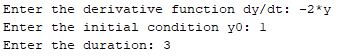
\includegraphics[]{images/input_ode.png}}
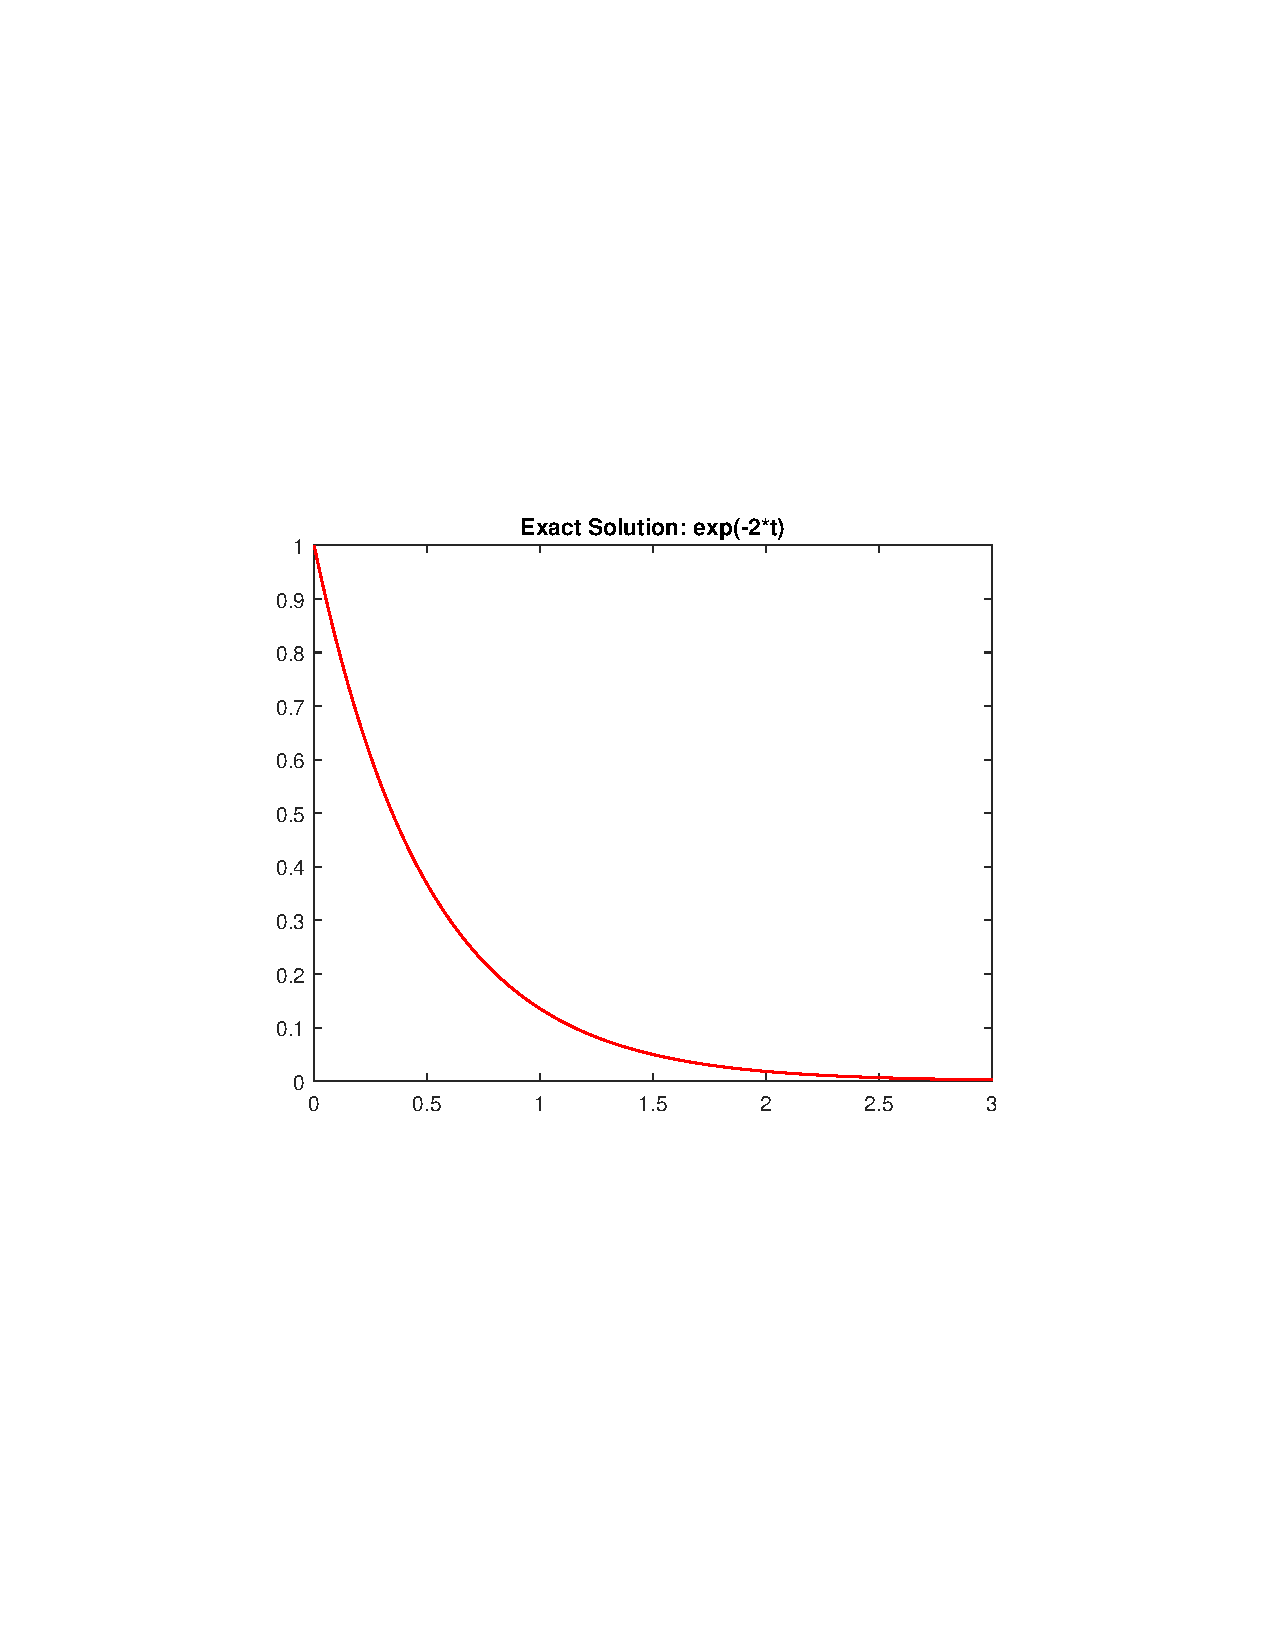
\includegraphics[trim={3.6cm 8.35cm 3.25cm 8cm},clip,scale=0.75]{pdfs/ode.pdf}
\end{center}


Differential equations have broad applications in diverse areas, including physics, engineering, biology, economics, and more. They provide a powerful framework for modeling dynamic systems, predicting behavior, and understanding the underlying principles governing various phenomena. By studying and analyzing differential equations, we can gain insights into the behavior and dynamics of real-world systems, making them an essential tool in scientific research and problem-solving.

\newpage
\subsection{Applications}

\subsubsection{Growth and Decay}
Growth and decay are fundamental concepts that occur in various natural and man-made systems. Whether it's the growth of a population, the decay of a radioactive substance, or the depreciation of an asset, understanding and modeling these processes are essential in many fields. Ordinary differential equations provide a powerful framework for studying growth and decay phenomena by expressing the rate of change of a quantity as a function of its current value.

By solving these equations, we can analyze the dynamics, predict future behavior, and make informed decisions. The application of ordinary differential equations to growth and decay processes enables us to gain insights into the underlying mechanisms and optimize outcomes in fields such as biology, economics, physics, and more.

Let's consider an example of population growth or decay using an ordinary differential equation. Suppose we have a population of bacteria, and we want to model the growth or decay of this population over time.

Let $N(t)$ represent the population size at time $t$. If we assume that the rate of change of the population is proportional to the population itself, we can express this relationship using the following ordinary differential equation:

\begin{gather*}
\dfrac{dN}{dt} = kN(t)\\
\text{where } k \text{ is constant that determines the growth or decay rate}
\end{gather*}

To solve this ordinary differential equation, we can separate the variables, integrate both sides, and then simplify by exponentiating both sides:

$$
\begin{aligned}
\dfrac{1}{N(t)} dN = kdt&\Rightarrow \int\dfrac{1}{N} dN = \int k dt\\
&\Leftrightarrow \ln|N(t)| = kt + C^*\\
&\Leftrightarrow N(t) = \pm e^{C^*}e^{kt} = Ce^{kt}\\
\end{aligned}
$$

The equation $N(t) = Ce^{kt}$ represents the general solution to the ordinary differential equation governing population growth or decay. The constant $C$ represents the initial population size at $t = 0$.

By specifying the initial condition $N(0) = N_0$, we can determine the particular solution for a specific scenario:

$$N(t) = N_0 e^{kt}$$

This equation allows us to predict the population size $N(t)$ at any given time t based on the initial population size $N_0$ and the growth or decay rate represented by the constant k.

In summary, ordinary differential equations provide a mathematical framework to model growth and decay processes in various systems, including population dynamics. By solving these equations, we can understand and predict the behavior of the system over time, making them valuable tools in the field of mathematical modeling and analysis.

\subsubsection{Pursuit Curve}

Pursuit curves find practical applications in various real-life scenarios, demonstrating the relevance of ordinary differential equations. One such application is in the field of aerospace engineering, particularly in the tracking and interception of flying objects. Consider a scenario where a rocket or a missile aims to intercept a target moving through space. By modeling the motion of the target and the rocket using differential equations, engineers can determine the trajectory that the rocket should follow to intercept the target successfully. The pursuit curve, derived from the solution of the differential equation, provides the desired path for the rocket to pursue and eventually reach the target.

Pursuit curves find applications in robotics and autonomous navigation, such as tracking moving targets for autonomous drones and self-driving cars. By using differential equations, engineers can develop algorithms to calculate optimal trajectories and maintain desired positions relative to the target, enabling accurate and efficient tracking.

In the field of animal behavior and predator-prey dynamics, pursuit curves offer insights into predator-prey interactions. Differential equations are used to model the movements of predators and prey, allowing ecologists and biologists to understand the strategies employed by predators and the evasive maneuvers adopted by prey. The pursuit curve derived from these equations sheds light on the dynamics of natural predator-prey relationships.

To gain a clearer understanding of this topic, we have developed a Matlab program that simulates the trajectories of two objects. By specifying a unit velocity vector for object 1 and the duration of the simulation, the program allows the second object to pursue and chase the first object, forming a pursuit curve. Below is the code:\\[-0.3cm]

\begin{minted}{matlab}
clc; clearvars;

% User input for the positions of points A and B
posA = input("Enter the position of point A [x, y]: ");
x1 = posA(1);
y1 = posA(2);
% User input for the vector A
A = input("Enter the vector A [x, y]: ");
A = A / norm(A);  % Convert A to a unit vector

posB = input("Enter the position of point B [x, y]: ");
x2 = posB(1);
y2 = posB(2);

% User input for the duration of the simulation
duration = input("Enter the duration of the simulation: ");

% Define the velocity of point A
v = 1;

% Set the time span
tspan = [0 duration];

% Define the initial conditions
initial_condition = [x1, y1, x2, y2];

% Solve the system of ordinary differential equations
[t, positions] = ode45(@(t, y) pursuitCurve(t, y, v, A), tspan, initial_condition);

% Extract the positions of points A and B
x1 = positions(:, 1);
y1 = positions(:, 2);
x2 = positions(:, 3);
y2 = positions(:, 4);

% Animate the pursuit curve
figure;
for i = 1:length(t)
    plot(x1(i), y1(i), 'ro', 'MarkerSize', 10, 'MarkerFaceColor', 'r');  % Point A
    hold on;
    plot(x2(i), y2(i), 'bo', 'MarkerSize', 10, 'MarkerFaceColor', 'b');  % Point B
    plot(x1(1:i), y1(1:i), 'r-', 'LineWidth', 2);  % Trajectory of point A
    plot(x2(1:i), y2(1:i), 'b--', 'LineWidth', 2);  % Trajectory of point B
    xlim([min([x1; x2])-1, max([x1; x2])+1]);
    ylim([min([y1; y2])-1, max([y1; y2])+1]);
    xlabel('x');
    ylabel('y');
    title('Pursuit Curve Simulation');
    grid on;
    hold off;
    pause(0.1);
end

% Function defining the system of ordinary differential equations
function dydt = pursuitCurve(~, y, v, A)
    x1 = y(1);
    y1 = y(2);
    x2 = y(3);
    y2 = y(4);
    
    dx1dt = v * A(1);
    dy1dt = v * A(2);
    dx2dt = (x1 - x2) / norm([x1 - x2, y1 - y2]);
    dy2dt = (y1 - y2) / norm([x1 - x2, y1 - y2]);
    
    dydt = [dx1dt; dy1dt; dx2dt; dy2dt];
end
\end{minted}

Input and Result:\\[-0.35cm]

\begin{center}
\efbox{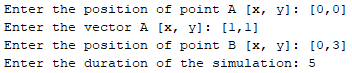
\includegraphics[]{images/input_pursuit_curve.png}}
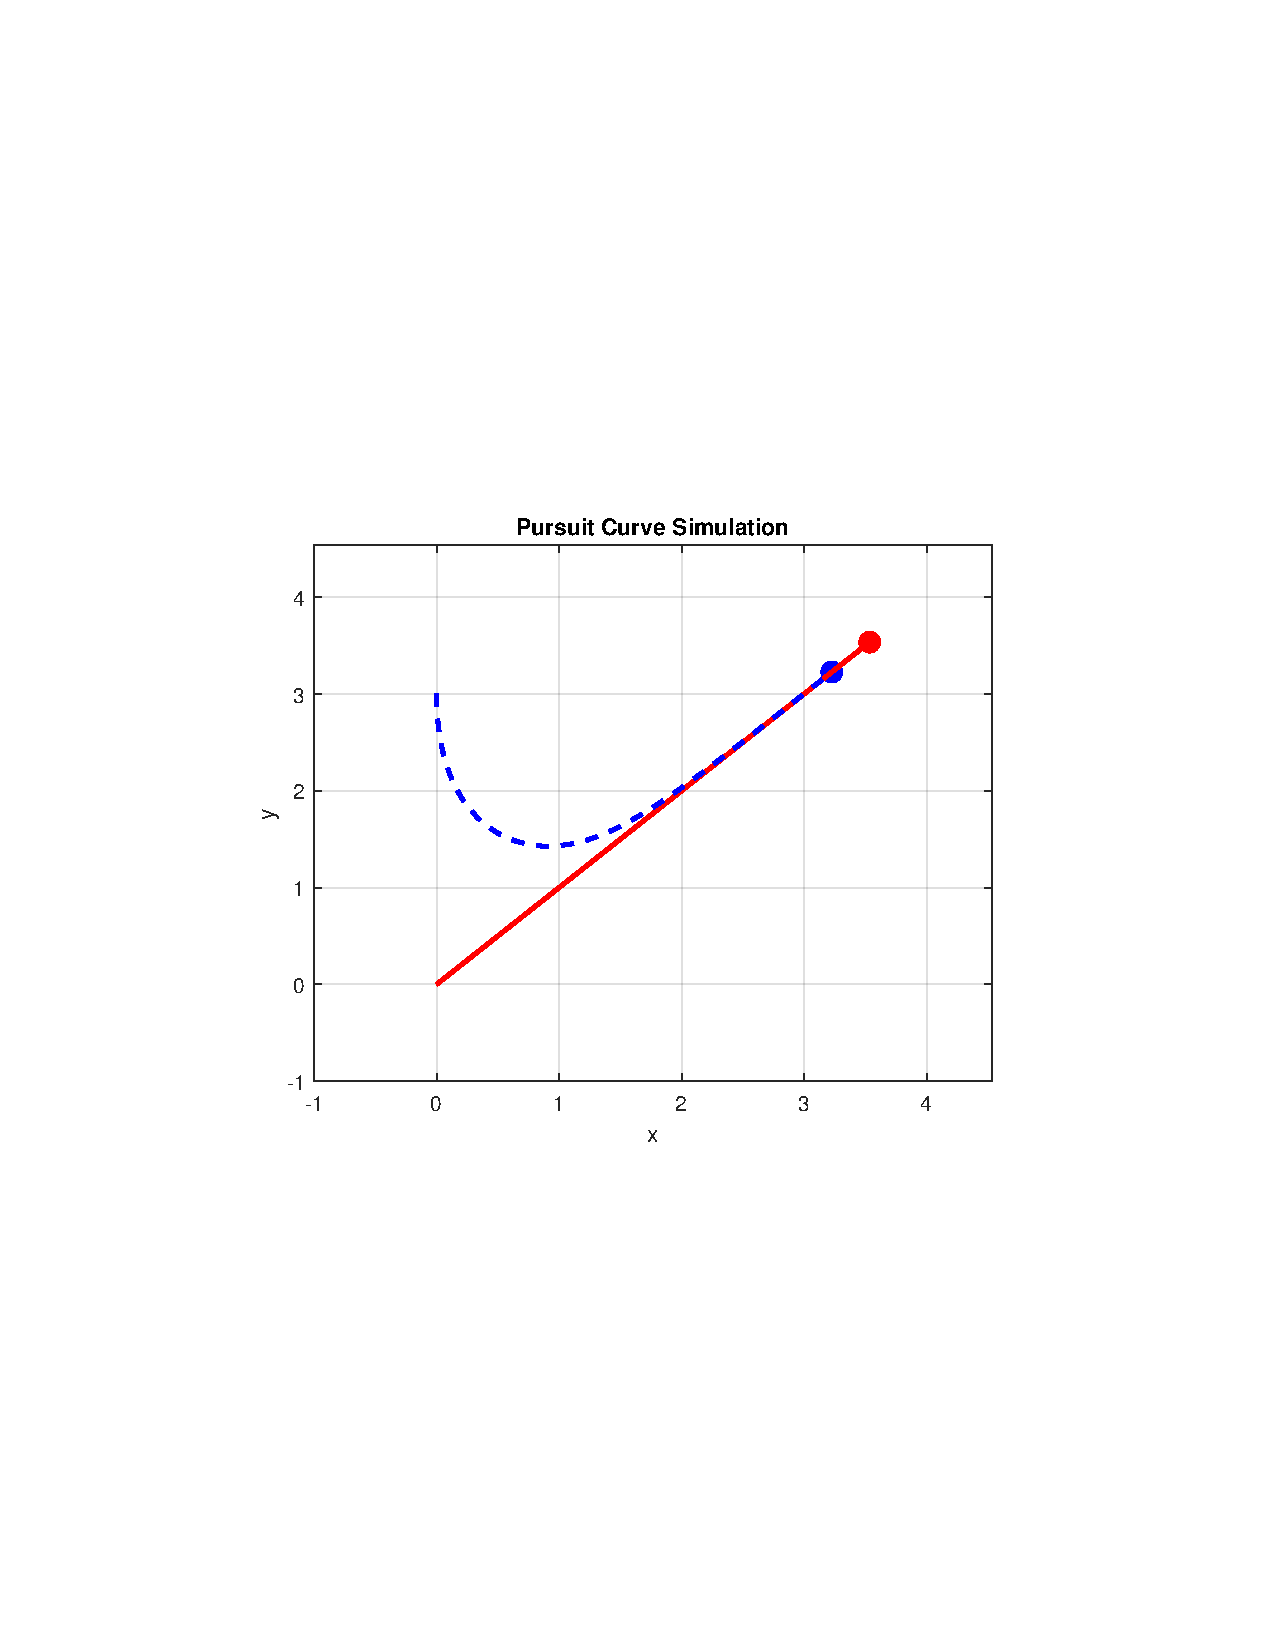
\includegraphics[trim={3.6cm 8.35cm 3.25cm 8cm},clip,scale=0.75]{pdfs/pursuit_curve.pdf}
\end{center}

In summary, pursuit curves derived from ordinary differential equations have practical applications in diverse fields such as aerospace engineering, robotics, and ecology. By formulating pursuit problems as differential equations, engineers and scientists can devise optimal strategies for tracking and intercepting targets, design autonomous systems capable of following moving objects, and gain insights into predator-prey dynamics. These real-life applications demonstrate the significance of differential equations and the pursuit curve concept in solving complex problems and understanding dynamic systems.

\subsubsection{Disease Prediction}

The $SEIR$ model is an extension of the $SIR$ model\footnote{Compartmental models in epidemiology: \url{https://en.wikipedia.org/wiki/Compartmental_models_in_epidemiology}} that incorporates an additional compartment to represent individuals who are Exposed ($E$) to the disease but not yet infectious. This model is particularly useful for studying diseases with an incubation period, such as COVID-19. The $SEIR$ model is based on a system of ordinary differential equations that describe the transitions between the compartments.

Let's consider an example of using the $SEIR$ model to make predictions about COVID-19. The following set of differential equations represents the $SEIR$ model:

$$
\begin{aligned}
\dfrac{dS}{dt} &= \mu-dS-\beta S I\\[0.2cm]
\dfrac{dE}{dt} &= \beta S I - (d+\alpha) E\\[0.2cm]
\dfrac{dI}{dt} &= \alpha E - (d+\gamma) I\\[0.2cm]
\dfrac{dR}{dt} &= \gamma I - dR\\[0.2cm]
\end{aligned}
$$

Here, $S(t)$, $E(t)$, $I(t)$, and $R(t)$ represent the number of susceptible, exposed, infected, and recovered individuals at time $t$, respectively. $\beta$ represents the effective contact rate, $\alpha$ represents the rate at which exposed individuals become infectious, and $\gamma$ represents the recovery rate. Here is the flow chart for $SEIR$ model:

\usetikzlibrary{arrows.meta,positioning}
\begin{center}
\begin{tikzpicture}[node distance=1.75cm and 1.5cm, auto,
>=Latex,every node/.append style={align=center}, 
int/.style={draw, minimum size=1.6cm}]
\node [int] (a) {$S$}; 
\node (b) [left of=a, coordinate] {a}; 
\node [int] (c) [right=of a] {$E$}; 
\node (c1) [below=of a, coordinate] {c1}; 
\node (c2) [below=of c, coordinate] {c2};
\node [int] (d) [right=of c] {$I$}; 
\node (c3) [below=of d, coordinate] {c3};
\node [int] (e) [right=of d] {$R$}; 
\node (c4) [below=of e, coordinate] {c4};
\path[->] (b) edge node {$\mu$} (a)
   (a) edge node {$\beta SI$} (c) edge node {$dS$} (c1)
   (c) edge node {$\alpha E$} (d) edge node {$dE$} (c2) 
   (d) edge node {$\gamma I$} (e)  edge node {$dI$} (c3)  
   (e) edge node {$dR$} (c4);    
\end{tikzpicture}
\end{center}

The $SEIR$ model is utilized to forecast the spread of diseases such as COVID-19. Estimating the model's parameters, including $\beta$, $\alpha$, and $\gamma$, is essential for achieving accurate predictions. Numerical integration techniques and solver functions in programming languages like Python are employed to solve the aforementioned model's differential equations.

Simulating the $SEIR$ model with estimated parameter values allows us to generate predictions for the future course of the outbreak. These predictions offer insights into factors such as the number of infections, the timing and duration of the peak, and the impact of interventions like vaccination and quarantine measures.

It is important to consider the limitations of the $SEIR$ model. Prediction accuracy depends on factors like data quality, model assumptions, and parameter uncertainties. Regular updates and refinement of the model with new data are necessary to improve prediction accuracy.

In summary, the $SEIR$ model is a valuable tool for predicting the spread of diseases like COVID-19. By estimating model parameters and numerically solving the differential equations, we can generate predictions that aid in understanding disease dynamics, evaluating control strategies, and informing public health interventions.

\newpage
\section{References}
\vspace{0.25cm}
    \begin{otherlanguage}{vietnamese}
        \nocite{*}%
        \printbibliography[heading=none]
    \end{otherlanguage}


\end{document}